% =====================================================================
%  Analog Game Design, lezione 14 — Gli strumenti dello sviluppo:
%  regolamento, revisioni e bilanciamento (lo sviluppo, seconda parte).
%  La seconda delle due lezioni di Marta, docente ospite, sviluppatrice
%  di giochi da tavolo. In apertura, la coda della lezione precedente:
%  il regolamento dello sviluppo (dal macro al micro, chiarezza,
%  integrità, consistenza strutturale, sintattica e terminologica,
%  prossimità) con la domanda di Rita sul linguaggio; i materiali
%  promozionali (USP, foto di metà partita, promo, tutorial per le
%  fiere); le revisioni (versionare, dividersi i compiti, la copia
%  zero). Poi la "cassetta degli attrezzi" dello sviluppo: principi
%  generali, analisi SWOT, personas, i sei cappelli per pensare. Dopo
%  la prima pausa, il bilanciamento: l'articolo di Richard Garfield
%  ("The Balancing Act"), lo spazio di gioco, costi e benefici, house
%  rules, per chi si bilancia (il "dio della simmetria", il gioco, il
%  target, esperti e principianti), perché non bilanciare in modo
%  matematico (e con l'IA), il bilanciamento esperienziale, i giochi a
%  scarsa interazione, il budget di complessità, le strategie ad alto
%  e basso rischio, l'ancoraggio (Stone Age). Dopo la seconda pausa:
%  il bilanciamento di durata, raddoppiare o dividere la risorsa, due
%  problemi e una soluzione, gli elementi ricorrenti (progressioni,
%  moltiplicazioni, set, esclusività, crescita, alea, probabilità),
%  smussare la stella, i "difetti" (player elimination, runaway e bash
%  the leader, feedback loop, kingmaking, convergenza, ordine di turno),
%  la domanda sulle sinergie, gli esempi (Carcassonne a tre tessere,
%  Bonsai, Magical Athlete, Party House).
%  Fonte: trascrizione della quattordicesima lezione (AGD14) del corso
%  breve di Analog Game Design, seconda edizione: una lezione online di
%  circa tre ore, con ogni probabilità venerdì 20 novembre 2026, tenuta
%  da Marta.
%  Pacchetti richiesti nel preambolo del libro (già presenti nel
%  main.tex): \usepackage{booktabs}, \usepackage{tikz} con
%    \usetikzlibrary{shapes.geometric,shapes.symbols,shapes.misc,
%      arrows.meta,positioning,calc,fit}
%  (le librerie vanno caricate nel preambolo, non nel capitolo).
%  Consigliati, come per gli altri capitoli: \usepackage[italian]{babel}
%  e \usepackage[T1]{fontenc} (il capitolo compila anche senza).
%
%  Collocazione nel libro: parte "Analog Game Design", quattordicesimo
%  capitolo (numerazione propria 2.14). Nel file principale del libro,
%  subito dopo il capitolo 2.13:
%
%    % =====================================================================
%  Analog Game Design, lezione 13 — Lo sviluppo (development) del gioco
%  analogico, prima parte.
%  La prima delle due lezioni di Marta, docente ospite, sviluppatrice di
%  giochi da tavolo da una decina d'anni. In apertura, con Daniele, una
%  coda di domande: quanto può cambiare un gioco dopo il pitch
%  (divergere e convergere, il tagliare), il calendario delle lezioni,
%  le difficoltà dei playtest e la narrativa combinatoria di Reigns per
%  il gruppo del roguelike in solitario. Poi il giro di presentazioni di
%  Marta (un gioco che ci piace con un difetto, uno che non ci piace con
%  un pregio) e le slide: che cos'è lo sviluppo (una mediazione tra
%  stakeholder) e che cosa non è; i tre principi (personale, armonico,
%  collaborativo) con la recensione di Space-Biff!; gli stakeholder;
%  design contro sviluppo; lo sviluppo come mestiere d'esperienza; il
%  rapporto tra designer e sviluppatrice (collaborazione attiva e
%  passiva, aspettative, fiducia); la storia del ruolo (SPI, Fantasy
%  Flight, alea, Hans im Glück; developer ed editor). Dopo la pausa: il
%  conflitto di interessi, le otto fasi dello sviluppo (selezione,
%  ricerca, concettualizzazione con il Game Concept Document,
%  presentazione con il caso The Faceless, testing, implementazione con
%  il bilanciamento e il sovrabilanciamento, preparazione degli asset;
%  le revisioni e il regolamento sono rimandati alla lezione
%  successiva), il caso Magical Athlete, Stonemaier, Oath, il target con
%  premi, Bartle e LeBlanc.
%  Fonte: trascrizione della tredicesima lezione (AGD13) del corso breve
%  di Analog Game Design, seconda edizione: una lezione online di circa
%  tre ore, con ogni probabilità lunedì 16 novembre 2026, tenuta da
%  Marta, con Daniele presente solo all'inizio.
%  Pacchetti richiesti nel preambolo del libro (già presenti nel
%  main.tex): \usepackage{booktabs}, \usepackage{tikz} con
%    \usetikzlibrary{shapes.geometric,shapes.symbols,shapes.misc,
%      arrows.meta,positioning,calc,fit}
%  (le librerie vanno caricate nel preambolo, non nel capitolo).
%  Consigliati, come per gli altri capitoli: \usepackage[italian]{babel}
%  e \usepackage[T1]{fontenc} (il capitolo compila anche senza).
%
%  Collocazione nel libro: parte "Analog Game Design", tredicesimo
%  capitolo (numerazione propria 2.13). Nel file principale del libro,
%  subito dopo il capitolo 2.12:
%
%    % =====================================================================
%  Analog Game Design, lezione 12 — Prototipi, regolamenti e raccolta
%  dei feedback.
%  Una lezione "tradizionale", con poche slide molto pratiche, tenuta da
%  Ruggero da solo, e poi una lunga parte aperta sui progetti di gruppo.
%  In apertura, l'attesa, le scadenze (tutoraggio, consegna, final
%  review) e la domanda su quanto un gioco possa cambiare dopo il pitch.
%  Poi le slide: che cos'è un prototipo e perché si fa (costo, tempo,
%  il muro psicologico del costo del cambiamento); il triangolo dei
%  prototipi (ruolo, look and feel, implementazione) preso da un paper
%  di elettronica, con gli esempi della scatola della pizza, delle
%  schermate stampate e del debug; il regolamento: come si insegna un
%  gioco, la facilitazione, pre-gioco e post-gioco, fiction e intenti,
%  la scrittura come medium lineare contro il gioco come ecosistema, gli
%  indici e i blocchi, che cosa c'è in un regolamento (di che cosa parla
%  il gioco, che cosa serve per giocare, i principi di gioco, con
%  l'esperimento sul ritematizzare Diamant); i metodi etnografici di
%  raccolta dei feedback (osservazione in presenza, registrazione,
%  nessuna osservazione; debriefing orale di gruppo, debriefing 1-1,
%  form chiuso, report libero), il sentimento dietro la soluzione, la
%  composizione del gruppo di playtest e il contesto. Infine le domande
%  (perché hai attaccato?, la ripetitività) e, dopo la pausa, lo stato
%  dei tre progetti: il gruppo di Rita bloccato nella ricerca, Murder
%  Memory e la storia che blocca il gioco, Automa e le carte da poker.
%  Fonte: trascrizione della dodicesima lezione (AGD12) del corso breve
%  di Analog Game Design, seconda edizione: una lezione online di circa
%  tre ore, con ogni probabilità venerdì 6 novembre 2026, tenuta da
%  Ruggero.
%  Pacchetti richiesti nel preambolo del libro (già presenti nel
%  main.tex): \usepackage{booktabs}, \usepackage{tikz} con
%    \usetikzlibrary{shapes.geometric,shapes.symbols,shapes.misc,
%      arrows.meta,positioning,calc,fit}
%  (le librerie vanno caricate nel preambolo, non nel capitolo).
%  Consigliati, come per gli altri capitoli: \usepackage[italian]{babel}
%  e \usepackage[T1]{fontenc} (il capitolo compila anche senza).
%
%  Collocazione nel libro: parte "Analog Game Design", dodicesimo
%  capitolo (numerazione propria 2.12). Nel file principale del libro,
%  subito dopo il capitolo 2.11:
%
%    % =====================================================================
%  Analog Game Design, lezione 11 — Il pitch dei progetti di gruppo.
%  Una lezione senza slide e senza lezione frontale: i tre gruppi del
%  corso presentano in tre minuti l'idea del gioco che svilupperanno
%  fino a dicembre, e i tre docenti (Daniele, Beatrice e Ruggero) fanno
%  domande, si ritirano a discutere in privato e poi restituiscono i
%  feedback. In apertura, l'attesa e le regole del pitch. Poi i tre
%  pitch, ciascuno con le sue domande: Murder Memory (escape room
%  investigativa da tavolo a squadre), La Peste (party game a ruoli
%  segreti ispirato alla Maschera della Morte Rossa), un gioco di ruolo
%  in solitario deck building, roguelike e journaling. Dopo la camera
%  di consiglio: la premessa ai feedback (indicazioni, non consigli; il
%  regolamento di massima per il 6 novembre), la domanda di Tiziana su
%  che cosa sia un regolamento in una escape room, i feedback gruppo
%  per gruppo con i casi studio assegnati, il legame tra obiettivo e
%  agency, il perché dei tre minuti, i giochi "generalisti". Infine le
%  domande aperte: scrivere il gioco per chi lo gioca senza di voi, la
%  curse of knowledge, la vergogna delle idee, e una lunga discussione
%  su roguelike, RNG e narrativa modulare (partire dalle emozioni, non
%  dai perk; le meccaniche come metafore; l'ortogonalità).
%  Fonte: trascrizione dell'undicesima lezione (AGD11) del corso breve
%  di Analog Game Design, seconda edizione: una lezione online di circa
%  tre ore, lunedì 12 ottobre 2026, condotta da Daniele con Beatrice e
%  Ruggero.
%  Pacchetti richiesti nel preambolo del libro (già presenti nel
%  main.tex): \usepackage{booktabs}, \usepackage{tikz} con
%    \usetikzlibrary{shapes.geometric,shapes.symbols,shapes.misc,
%      arrows.meta,positioning,calc,fit}
%  (le librerie vanno caricate nel preambolo, non nel capitolo).
%  Consigliati, come per gli altri capitoli: \usepackage[italian]{babel}
%  e \usepackage[T1]{fontenc} (il capitolo compila anche senza).
%
%  Collocazione nel libro: parte "Analog Game Design", undicesimo
%  capitolo (numerazione propria 2.11). Nel file principale del libro,
%  subito dopo il capitolo 2.10:
%
%    \input{AGD/AGD10_ux_design_e_paragame}
%    \input{AGD/AGD11_pitch_e_feedback}
%
%  Tutte le etichette di questo capitolo hanno il prefisso "a11:"
%  (a11:cap:..., a11:sec:..., a11:fig:..., a11:tab:...). Il capitolo è
%  autonomo: non contiene \ref verso altri capitoli.
%  Le figure e le tabelle sono ricostruzioni schematiche di quanto
%  detto a voce (la lezione non ha slide dei docenti), non copie delle
%  slide dei gruppi. Dove la trascrizione è troppo rovinata per
%  ricostruire un dettaglio (un nome di gioco, chi sta parlando), il
%  capitolo lo dice invece di inventarlo.
% =====================================================================

\chapter[Il pitch dei progetti di gruppo]{Il pitch dei progetti di gruppo: tre
giochi, tre minuti, e i feedback di chi li dovrà giocare}
\label{a11:cap:pitch}

Questa è l'\textbf{undicesima lezione} del corso di \textbf{Analog Game Design}, ed è
diversa da tutte le precedenti. ``Non abbiamo slide, non abbiamo una lezione, nel senso
di lezione frontale'': oggi è il giorno del \textbf{\emph{pitch}}, quello che Ruggero, a
fine della lezione sul paragame, aveva dato per certo come ``il 12'', che ``sta nella
pietra''. I tre gruppi di lavoro del corso presentano in \textbf{tre minuti} l'idea del
gioco che svilupperanno fino a dicembre; dopo ogni presentazione i docenti fanno
qualche minuto di domande, poi il gruppo esce dalla stanza virtuale e i docenti
discutono in privato. Quando tutti e tre i gruppi hanno presentato, la seconda metà della
lezione è dedicata ``solo ai feedback, esclusivamente ai feedback''.

I tre progetti sono molto diversi tra loro. Il primo, \textbf{\emph{Murder Memory}}, è
una \emph{escape room} investigativa da tavolo in cui due squadre, la polizia e un
indiziato che ha perso la memoria, risolvono enigmi in parallelo fino a un
interrogatorio finale. Il secondo, \textbf{\emph{La Peste}}, è un \emph{party game} a
ruoli segreti, di deduzione e \emph{bluff}, ambientato nel ballo della \emph{Maschera
della Morte Rossa} di Edgar Allan Poe: a ogni rintocco dell'orologio si balla, ci si
scambiano le carte e la malattia si diffonde. Il terzo è un \textbf{gioco di ruolo in
solitario}, \emph{deck building}, \emph{roguelike} e di \emph{journaling}: si
sopravvive il più a lungo possibile tenendo in equilibrio corpo, mente e status
sociale di un personaggio, e alla fine della partita resta la sua storia, da scrivere.

I feedback sono franchi, e i docenti lo dicono subito: non saranno ``consigli'' ma, dove
l'esperienza dice che un gruppo si sta infilando in un ``ginepraio troppo grosso per il
periodo di tempo che avete'', \textbf{indicazioni} precise (``non fate questo, fate
questo''). I temi che ritornano per tutti e tre i gruppi sono pochi e molto concreti:
\textbf{convergere} su un'idea e uno \emph{scope} realizzabili, \textbf{scrivere il
regolamento} (``il vostro gioco lo devono poter giocare altre persone che non sono
voi''), collegare l'\textbf{obiettivo} di chi gioca a ciò che fa \textbf{turno per
turno}, partire dalle \textbf{emozioni} e non dai bilanciamenti, e usare i
\textbf{casi studio} come strumenti di \emph{problem solving}, non come modelli da
copiare. Ogni gruppo riceve una lista di giochi da studiare, in tutto più di quindici
titoli (tabella~\ref{a11:tab:reference}). L'ultima parte della lezione, aperta alle
domande, diventa una lunga discussione su \emph{roguelike}, generazione casuale e
narrativa modulare, temi che due dei docenti praticano per mestiere.

La lezione è \textbf{online}, su Zoom, e si tiene \textbf{lunedì 12 ottobre
2026}\footnote{La data è quella fissata nella lezione precedente (``il 12 sta nella
pietra'', e ``lunedì'' sono i \emph{pitch}). In questa lezione Daniele ricorda che
Gianmarco ``di solito lunedì arriva un'ora dopo per motivi di lavoro''.}, presumibilmente
dalle 17 alle 20 come le altre: Daniele, che arriva ``da sei ore di lezioni'', ne fa
``altre tre di fila'' e a fine serata parla della sua ``nona ora''. La conducono insieme
i tre docenti del corso: \textbf{Daniele}, che scandisce i tempi, fa partire il timer e
gestisce la sala d'attesa; \textbf{Beatrice} (``Bea''); e \textbf{Ruggero}. Gli studenti
sono divisi in tre gruppi: \textbf{Tiziana}, \textbf{Angelo} e \textbf{Lorenzo L.}
(\emph{Murder Memory}); \textbf{Tancredi}, \textbf{Gianmarco} e \textbf{Lorenzo}
(\emph{La Peste})\footnote{Nel corso ci sono due Lorenzo, e la trascrizione li
distingue solo in un punto, quando Daniele presenta il primo gruppo come ``Tiziana,
Lorenzo L. e Angelo''. L'altro Lorenzo è nel gruppo di Tancredi e Gianmarco (``io sono
con Gianmarco e Lorenzo'', dice Tancredi). Il capitolo scrive ``Lorenzo L.'' per il
primo e ``Lorenzo'' per il secondo.}; \textbf{Giordano}, \textbf{Nicola} e
\textbf{Rita} (il \emph{roguelike} in solitario)\footnote{Il nome di Rita è storpiato in
``Verità'' (``Giordano, Nicola, Verità'') e in ``Piano'' (``Rita, Piano e Nicola''); il
contesto e un successivo ``ha ragione anche Rita'' lo rendono sicuro.}.

Tre avvertenze di lettura, le stesse dei capitoli precedenti. La prima: la trascrizione è
automatica e storpia moltissimi nomi. Ruggero diventa ``Ruger'', ``Rugger'',
``Brugger'' e ``Rugg''; \emph{Murder Memory} diventa ``Merd Memory'', ``Mordor
Memory'', ``Marder Memory'' e ``Mordere Memory''; \emph{Lupus in Tabula} è ``Lupus in
Fabula'', ``l'Opus in Fabula'' e ``l'upus in tabula''; \emph{Slay the Spire} è ``Slade
of Spire'', ``Slade Spire'', ``Zade Spyder'' e ``As Lady Spire 2''; \emph{Reigns} è
``Rains'', ``Rain'' e ``Reins''; \emph{The Quiet Year} è ``The Quiet Ear'', ``White
Tier'', ``quai tier'' e ``quietire''; \emph{Inhuman Conditions} è ``In Human
Condition'', ``Unicondition'' e ``Non è un Condition''; Tabletop Simulator è ``Temporal
Simulator'' e ``Voltoltor Simulator''. Dove la ricostruzione è sicura, o molto probabile,
il capitolo usa la forma corretta e lo segnala in nota la prima volta; dove non lo è,
riporta la forma della trascrizione e lo dice. La seconda: con tre docenti e dieci
studenti che parlano spesso uno sull'altro, la trascrizione quasi mai segnala chi sta
parlando, e in più punti ripete due volte la stessa frase (un artefatto del
riconoscimento vocale, che il capitolo ignora). Il capitolo attribuisce le frasi quando
il contesto lo rende chiaro (chi viene chiamato per nome, chi dice ``io sto creando un
\emph{roguelike}'', chi ha scansionato un libro) e resta generico altrimenti. La terza:
le slide dei gruppi non sono nella trascrizione; il capitolo ricostruisce i giochi da ciò
che i gruppi dicono a voce, nelle presentazioni e nelle risposte.

\paragraph{Come leggere questo capitolo.} I tre progetti sono descritti per come sono
stati presentati il 12 ottobre: idee in fase embrionale, con parti ``ancora da
definire'' che i gruppi stessi segnalano. Il capitolo non le completa e non le corregge:
riporta le domande che i docenti fanno, le risposte, e poi i feedback. Le figure
ricostruiscono gli schemi che emergono dal discorso (la procedura del \emph{pitch}, il
round della \emph{Peste}, il legame tra obiettivo e \emph{agency}, il calendario fino a
dicembre); le tabelle riassumono i progetti e i casi studio. Qua e là, dei paragrafi di
\textbf{approfondimento} collegano la lezione ai libri di game design di riferimento
(soprattutto \emph{The Art of Game Design} di Jesse Schell e \emph{A Theory of Fun} di
Raph Koster) e a qualche nozione di psicologia della comunicazione; sono segnalati come
tali e non fanno parte della lezione.

Il percorso del capitolo segue quello della lezione:
\begin{enumerate}
  \item l'attesa, la logistica e le \textbf{regole del \emph{pitch}} (sezioni
        \ref{a11:sec:attesa} e~\ref{a11:sec:regole});
  \item i tre \emph{pitch}, ciascuno con le sue domande: \emph{Murder Memory},
        \emph{La Peste}, il \emph{roguelike} di \emph{journaling} (sezioni
        da~\ref{a11:sec:murder} a~\ref{a11:sec:roguelike});
  \item dopo la camera di consiglio, la \textbf{premessa ai feedback} e la domanda su
        \textbf{che cos'è un regolamento} (sezioni \ref{a11:sec:premessa}
        e~\ref{a11:sec:regolamento});
  \item i \textbf{feedback} gruppo per gruppo, con i casi studio (sezioni
        da~\ref{a11:sec:fbmurder} a~\ref{a11:sec:reference});
  \item le \textbf{domande aperte}: il regolamento come strumento di test, la
        \emph{curse of knowledge}, la vergogna delle idee (sezioni
        \ref{a11:sec:testing} e~\ref{a11:sec:vergogna});
  \item la discussione su \textbf{\emph{roguelike}, RNG e narrativa modulare}, e la
        chiusura (sezioni da~\ref{a11:sec:rng} a~\ref{a11:sec:chiusura}).
\end{enumerate}

% ---------------------------------------------------------------------
\section{L'attesa: una ``quotina di ansia''}
\label{a11:sec:attesa}

I primi a collegarsi sono Angelo, Nicola, Lorenzo e Rita; Beatrice e Ruggero sono già
in stanza. Daniele ``arriva un attimino in ritardo perché sta chiudendo un'altra
lezione''. La prima domanda è quella di sempre, ``come state? come vi sentite oggi?'', e
la risposta di uno studente riassume l'umore della classe: ``leggermente preoccupato
per il \emph{pitch}, ma se no tranquillo''. ``Anch'io, è normale'', gli risponde
Beatrice: ``ogni presentazione ha una quotina di ansia''. Lei, dice, è ``molto curiosa''
e ``abbastanza fiduciosa che usciranno bellissimi \emph{pitch}'': ``non preoccupatevi,
siamo proprio in ascolto anche per darvi una mano dove possiamo''. Poi va a prendere
``il mio quadernino di appunti, così mi segno le cose''.

In attesa dei ritardatari, i docenti aprono come al solito lo spazio per le domande,
magari di chi ha recuperato la lezione precedente. Uno studente la sta finendo di
recuperare: ``è una figata pazzesca''. Ruggero conferma che ``sulla questione del
paragame c'è tantissimo da dire'' e spera che abbia dato ``qualche spunto''. Poi spiega
la logistica, che ``già dovreste sapere'': niente slide e niente lezione frontale; ``oggi
vediamo i vostri \emph{pitch} e dedichiamo il tempo a ciascun gruppo''. Si corregge
subito dopo un lapsus (``dedichiamo il gruppo a ciascun tempo. Chi può dirlo? Qualcuno
finirà nell'800, qualcuno finirà nel 2000''). L'idea è di dare ai gruppi dei feedback
``in base anche al vostro \emph{pitch}''.

Arriva Daniele, accolto con un ``grazie in fanfare'': viene ``da sei ore di lezioni''
(``e invece adesso guarda, ne fai altre tre di fila''; ``Madonna, Daniele, ci lasci le
penne. Non svenire''). È lui a segnare le presenze. Arriva Tiziana, poi Tancredi. Mentre
manda ``due messaggi di lavoro'', Daniele dà un consiglio organizzativo: decidete ``dietro
le quinte'' l'ordine di presentazione dei gruppi, altrimenti lo sceglieranno i docenti.
Un vincolo c'è già: il gruppo di \textbf{Gianmarco}, Tancredi e Lorenzo va lasciato per
ultimo, perché Gianmarco il lunedì arriva circa un'ora dopo per lavoro (``tra una
quarantina di minuti massimo''). Un altro vincolo arriva da una studentessa del primo
gruppo, che deve staccarsi dieci minuti prima per prendere il treno delle otto: il suo
gruppo, se i compagni sono d'accordo (``Sì, sì, va bene''), può andare per primo. E
così si fa: ``iniziamo voi''.

Nel frattempo, il silenzio. ``Avremo l'\emph{horror vacui}'', scherza Ruggero: ``se
nessuno fa domande, io non so gestire. Daniele, cosa devo fare? Come faccio?''. Mancano
soltanto Giordano e Gianmarco; Daniele chiede di avvisarlo se entrano mentre i gruppi
presentano, così da non perdere le loro presenze.

C'è un ultimo intoppo tecnico, quello di ogni lezione online: la condivisione dello
schermo da un Mac (``il problema sempre del Mac per le autorizzazioni''). Daniele
sospetta un aggiornamento di Zoom (``e l'aula è diversa, tra l'altro: voi non ve ne
rendete conto, ma è un'aula differente''), ma alla fine la presentazione del primo
gruppo parte, in modalità ``presenta'', a schermo intero, con le frecce della tastiera
per andare avanti.

% ---------------------------------------------------------------------
\section{Le regole del \emph{pitch}}
\label{a11:sec:regole}

Prima di cominciare, Daniele ripete ``bene le regole del \emph{pitch} di oggi''
(figura~\ref{a11:fig:procedura}).

\begin{itemize}
  \item \textbf{Tre minuti.} Daniele fa partire un timer, conta ``3, 2, 1, via'', e il
        gruppo spiega ``tutto''. Chi va oltre non viene interrotto (``vi faccio
        finire''), ma alla fine si sentirà dire se è andato ``troppo lungo'' o ``troppo
        corto'', ``perché comunque sapevate che più o meno il tempo era quello''. Il
        tempo è uguale per tutti: ``non possiamo dare la possibilità a ogni team di
        avere più tempo rispetto agli altri. Altrimenti, è un casino''.
  \item \textbf{Due o tre minuti di domande} da parte di Daniele, Ruggero e Beatrice
        (``comunque quanto tempo ci mettono'').
  \item \textbf{La sala d'attesa.} Il gruppo esce da Zoom e rientra: Daniele ha
        attivato la sala d'attesa. I tre docenti si prendono ``qualche appunto in
        privato di confronto, senza essere registrati'', e poi riammettono tutti.
        Quando una studentessa chiede se la sala d'attesa sia ``una stanza che c'è
        veramente'', la risposta è che è ``l'anticamera'' di Zoom, dove però non si
        può parlare: chi vuole chiacchierare nel frattempo ha un canale vocale
        ``Analog Game Design'' sul Discord del corso.
  \item Si fa così per tutti i gruppi. La parte dei \emph{pitch} ``di solito dura
        un'ora, un'ora e mezza''; poi ``vi diamo i feedback e vi diamo anche dei
        consigli su cosa fare, perché poi dovrete svilupparle, 'ste robe''.
  \item \textbf{Il materiale.} Dopo ogni presentazione il gruppo condivide in chat il
        link alle slide (``Condividi'', ``chiunque abbia il link'', copia, incolla) e
        carica tutto nella cartella \emph{project work} del proprio gruppo.
\end{itemize}

Il primo gruppo avverte che improvviserà (``non ci siamo preparati sulla
presentazione''). Nessun problema, ma conviene che parli una persona sola, se ne ha una
che ``sa tutto quanto''; gli altri intervengono se manca qualcosa. Le domande dei
docenti, durante il primo \emph{pitch}, si allungano: alla fine il primo gruppo occupa
venti minuti, e Daniele stabilisce per gli altri ``venti minuti più o meno a team''.
Nessun feedback a caldo, nemmeno per chi deve andarsene prima: i docenti vogliono prima
``vedere il livello di tutti'', ``cosa hanno prodotto tutti''.

\begin{figure}[htbp]
\centering
\begin{tikzpicture}[
  font=\small,
  a11step/.style={draw, thick, rounded corners=3pt, minimum height=1.2cm,
               text width=2.3cm, align=center},
  a11priv/.style={draw, thick, dashed, rounded corners=3pt, fill=gray!15,
               minimum height=1.2cm, text width=2.3cm, align=center},
  a11arr/.style={-{Stealth[length=3mm]}, thick}
]
  \node[a11step] (a) {\textbf{Pitch}\\3 minuti\\a timer};
  \node[a11step, right=0.6cm of a] (b) {\textbf{Domande}\\2--3 minuti\\dei docenti};
  \node[a11priv, right=0.6cm of b] (c) {\textbf{Sala d'attesa}\\appunti dei\\docenti, non
    registrati};
  \node[a11step, right=0.6cm of c] (d) {\textbf{Rientro}\\e prossimo\\gruppo};
  \draw[a11arr] (a) -- (b);
  \draw[a11arr] (b) -- (c);
  \draw[a11arr] (c) -- (d);
  \draw[a11arr, rounded corners=4pt] (d.south) -- ++(0,-0.7) -| node[pos=0.25, below,
    font=\footnotesize]{per ognuno dei tre gruppi (circa 20 minuti a gruppo)} (a.south);
  \node[a11step, below=1.9cm of c, text width=5.2cm, fill=gray!5] (f)
    {\textbf{Seconda metà della lezione}\\feedback di gruppo, feedback di classe,
     domande aperte};
  \draw[a11arr, dashed] (d.east) -- ++(0.4,0) |- (f.east);
\end{tikzpicture}
\caption{La procedura del \emph{pitch} come la descrive Daniele. I feedback non arrivano
a caldo: i docenti li danno solo dopo aver visto tutti e tre i gruppi.}
\label{a11:fig:procedura}
\end{figure}

\paragraph{Approfondimento: il \emph{pitch} come prova di comunicazione.} Il formato
non è arbitrario, e Daniele lo spiegherà più avanti (sezione~\ref{a11:sec:fbpeste}):
tre minuti sono più o meno il tempo che un editore o un passante in fiera concede a
un'idea. Ma il \emph{pitch} è anche il primo momento in cui il gioco esce dalla testa del
gruppo e arriva a qualcuno che non c'era quando è stato pensato. Schell, in \emph{The Art
of Game Design}, dedica a questo passaggio un capitolo intero (``The Designer Gives the
Client a Pitch''), con l'idea di fondo che presentare un gioco serve anche a chi lo
presenta: costringe a scegliere che cosa, del gioco, conta davvero. Le domande dei docenti che seguono ogni \emph{pitch} di questa lezione
sono, in gran parte, la verifica di questo: che cosa faccio, io che gioco, in questo
momento?

% ---------------------------------------------------------------------
\section{Primo \emph{pitch}: \emph{Murder Memory}}
\label{a11:sec:murder}

Il primo gruppo è quello di \textbf{Tiziana}, \textbf{Lorenzo L.} e \textbf{Angelo}.
Presenta Tiziana, con l'accordo dei compagni, che interverranno se lei dimentica
qualcosa. Beatrice è ``già curiosissima di questo \emph{Murder Memory}'', e quando
lascia scappare un ``ho visto che è un gioco di carte'' viene fermata: ``non ci si
spoilera''. ``3, 2, 1, via.''

\subsection{Il \emph{pitch}}

\emph{Murder Memory} è ``una \emph{escape room} investigativa da tavolo'' (``ci siamo
dimenticati di precisare questa cosa, ma sarà da tavolo''). Chi gioca si trova coinvolto
in una \textbf{festa nella villa di un ricco proprietario}, durante la quale uno degli
invitati viene ucciso. Il principale indiziato è un altro invitato, che ha perso i sensi
e si sveglia \textbf{senza memoria}.

È un gioco \textbf{competitivo e cooperativo} insieme: due squadre si affrontano per
arrivare alla verità entro un \textbf{tempo limitato}, cooperando al loro interno.
\begin{itemize}
  \item Una squadra interpreta l'\textbf{indiziato} che ha perso la memoria. Non ricorda
        chi è né che cosa sia successo; potrebbe essere l'assassino e non saperlo. Si
        nasconde dalla polizia mentre cerca la verità, il che lo rende ancora di più il
        principale indiziato. ``Enigma dopo enigma'' deve scoprire chi è e svelare il
        mistero: ``è davvero lui il colpevole, o è solo un'altra vittima?''. Ogni
        giocatore della squadra potrebbe interpretare \textbf{un aspetto diverso della
        stessa persona}: è una cosa ``ancora da definire'', perché il gruppo non sa
        ancora se riuscirà a realizzarla in concreto.
  \item L'altra squadra interpreta i \textbf{poliziotti}, chiamati dal proprietario.
        Seguono le indagini, cercano indizi e interrogano gli invitati e il
        proprietario della villa, anche a proposito dell'indiziato che non riescono a
        trovare.
\end{itemize}

La struttura è una \textbf{successione lineare di enigmi}, che guida ciascuna squadra
alla risoluzione finale; la risoluzione prevede un \textbf{confronto diretto} tra le due
squadre, attraverso un \textbf{interrogatorio}. Il gruppo vorrebbe diversificare il più
possibile gli enigmi della successione, così da far partecipare più giocatori.
L'obiettivo dell'indiziato è scoprire la verità su se stesso e su ciò che è successo;
quello dei poliziotti, trovare il colpevole.

L'obiettivo del gruppo, come designer, è ``esprimere noi stessi ed esplorare nuove
tipologie di gioco'', fondendo elementi investigativi e di gioco di ruolo con la
struttura dell'\emph{escape}; e ``non ci dispiacerebbe pubblicarlo''. Le
\textbf{emozioni} che vogliono suscitare sono \textbf{incertezza}, \textbf{scoperta},
un'esperienza \textbf{adrenalinica}, \textbf{sorpresa} e \textbf{ansia}. Chiude una
battuta (``prenotatevi per provarlo, nessuno vi picchierà'') e la presentazione dei
membri del gruppo, ognuno con un nome da personaggio\footnote{La trascrizione riporta
``siamo Lorenzo, la Pomarda, Angelo, Tenente Colombo e io, Tiziana Carabayt'': almeno
``Tenente Colombo'' è chiaramente un soprannome scherzoso a tema investigativo; le
altre parole non sono ricostruibili con sicurezza.}.

Tempo: \textbf{tre minuti e quattordici secondi}. ``Direi che siamo comunque in
\emph{time}'', commenta Daniele: con un po' più di velocità ci sarebbero stati
tranquillamente.

\subsection{Le domande}

\paragraph{Come si vince?} Daniele parte con un apprezzamento e un dubbio. ``Lato
emotivo, molto bene'': le emozioni sono chiare. ``Lato meccanico, ho un po' di dubbi.''
Non è chiaro se il gioco abbia un \textbf{\emph{endgame} predefinito}, cioè se a livello
meccanico si vinca o si perda (``com'è che so se ho vinto o se ho perso?''), o se vada
``nella direzione più RPG'', in cui conta non chi vince ma ``avere un epilogo
strutturato''.

\paragraph{Chi risolve gli enigmi?} Un'altra domanda, più pragmatica, arriva dai docenti
insieme: le squadre sono due, ma gli enigmi chi li risolve? Insieme? Una squadra sola
mentre l'altra aspetta? (``Hanno due serie diverse.'') Il punto, chiarisce chi chiede, è
che non è chiaro ``che cosa faccio, in base al ruolo in cui sono'', e con quale obiettivo
personale al tavolo. Gli studenti non sapevano se dovessero entrare in questo dettaglio
nel \emph{pitch}; la risposta dei docenti è: se la risposta c'è, ditela; se non c'è,
``non generatela adesso''.

La risposta c'è. Gli enigmi procedono \textbf{in contemporanea}, con lo stesso tempo per
entrambe le squadre. I poliziotti hanno tutte le informazioni se riescono ad arrivare
alla fine del loro percorso; l'indiziato, arrivando alla fine del suo o il più vicino
possibile, ottiene informazioni su se stesso. \textbf{Allo scadere del tempo} le due
squadre si confrontano: i poliziotti fanno all'indiziato delle domande ``ovviamente
previste'', e l'indiziato saprà rispondere più o meno correttamente a seconda di quanto
ha scoperto. Se non sa chi è, ``rischia di rimanere un po' così'' su certe domande:
può inventarsi le risposte, ma rischia di non essere coerente. Ne nascono diversi esiti
(tabella~\ref{a11:tab:esiti}).

\begin{table}[htbp]
\centering
\small
\begin{tabular}{@{}p{5.6cm}p{7.4cm}@{}}
\toprule
\textbf{Situazione allo scadere del tempo} & \textbf{Esito (come descritto nel
\emph{pitch})} \\
\midrule
Entrambe le squadre arrivano alla fine del percorso & ``vincono entrambi'': i
poliziotti hanno gli elementi per capire chi è il vero colpevole, e l'indiziato sa
rispondere \\
I poliziotti arrivano alla fine, l'indiziato no & vincono i poliziotti: l'indiziato non
risponde correttamente alle domande e viene arrestato \\
L'indiziato ottiene le informazioni su di sé & l'indiziato vince: risponde correttamente
e viene scagionato \\
\bottomrule
\end{tabular}
\caption{Gli esiti dell'interrogatorio finale di \emph{Murder Memory}, come li descrive
Tiziana rispondendo alle domande. Il gruppo li presenta come idea ancora aperta.}
\label{a11:tab:esiti}
\end{table}

\paragraph{Quanti giocatori?} Daniele ha ``due domande molto brevi''. La prima: per
quanti giocatori è il gioco? Minimo due, uno per squadra; il gruppo pensava a un massimo
di \textbf{quattro per squadra}. Si interpretano solo i membri delle squadre? Sì: gli
invitati sono \textbf{NPC}. La seconda domanda, a Daniele, sfugge (``la sto perdendo?
Arrivo''); Beatrice lo rassicura (``è normale, poi tornano le domande mentre si
parla'') e prende la parola.

\paragraph{L'indiziato vuole scagionarsi o sapere la verità?} Beatrice ha ``tantissime
domande'' e ne seleziona alcune. La prima: la squadra dell'indiziato ha più lo scopo di
scagionarsi o di ricostruire la verità? Deve scoprire la verità su se stesso, risponde
Tiziana: scoprendo chi è, può affrontare i poliziotti. Beatrice chiede allora conferma
di un punto di design: si parte dall'idea che l'indiziato \textbf{non è colpevole}?
Corretto: non è colpevole, ``però non lo sa''.

\paragraph{Le sfaccettature dell'indiziato.} La seconda domanda di Beatrice riguarda le
``varie modalità di essere'' dell'indiziato, una per giocatore. Come funzionerà? Il
dubbio di Beatrice è più ampio: ``avete tanta carne al fuoco''. Enigmi, \emph{drive}
narrativi, una storia raccontata in più versioni, una polizia che non è una persona sola.
``Non vi sto invitando per forza a ridurre lo \emph{scope}'', ma ``è bene che abbiate una
direzione e una motivazione per tutte le scelte che prendete''. L'idea dell'indiziato
interpretato da una squadra intera le piace molto, ma non capisce che cosa farà lei,
giocando l'indiziato, oltre al lavoro di ricerca con le altre parti di sé: e quando
dovrà scagionarsi, come funzionerà? ``Compileremo una scheda, oppure parleremo con la
polizia?''. La risposta: la \textbf{mente divisa} era un'ipotesi iniziale, ``quasi
necessaria'' per giustificare più persone che fanno un'unica persona, ma non
obbligatoria, perché ``è nostra intenzione semplificare, non complicarci la vita''.

\paragraph{``Dovete spoilerare''.} A questo punto il gruppo ammette che manca una parte,
taciuta apposta ``perché non volevamo spoilerare''. La reazione dei docenti è immediata:
``Dovete spoilerare. Non siamo giocatori''. Al \emph{pitch} i docenti sono come un
\emph{publisher} a cui si propone un gioco: se non gli si dicono le cose importanti,
``noi come facciamo?''. ``Non lo sapevamo. Scusate.'' ``Tutto bene. Dici tutto adesso.''

Il retroscena è questo. Il \textbf{proprietario} della villa è un \textbf{appassionato di
enigmi} ed è lui \textbf{l'assassino}: ha ucciso uno degli invitati per costruire tutta
la messa in scena, ``fondamentalmente per divertirsi''. È lui a far perdere la memoria
all'indiziato, facendogli bere qualcosa. L'indiziato si sveglia in un punto in cui non è
visto, si accorge che è successo qualcosa (c'è la polizia) e va subito in agitazione:
non ricorda chi è, e se gli fanno una domanda non saprà cosa rispondere. Mentre si
nasconde trova \textbf{un oggetto che gli è familiare}, e da lì parte la serie degli
enigmi. Ha la sensazione di essere \textbf{guidato}, pilotato, che ci sia qualcosa che
non torna, ma ``non è il momento'' di chiederselo. Dall'altra parte, il proprietario
chiama i poliziotti e si diverte anche alle loro spalle: li guida attraverso altri
enigmi, con cui ricostruiscono le informazioni sugli invitati e, attraverso gli invitati,
sull'indiziato che non trovano. ``Scusa, no, è importantissimo'', commentano i docenti.

\paragraph{Storia prefatta o emergente?} Daniele fa un'ultima domanda, ``molto
semplice'': il gioco ha una \textbf{storia prefatta}, definita, che i giocatori stanno
solo scoprendo? Non è una storia emergente? Sì, è prefatta.

\paragraph{I giochi più vicini.} Poi tocca a Ruggero, con una domanda ``apparentemente
dal nulla'', le cui ragioni verranno dette dopo: nella fase di ricerca e sviluppo, quali
sono i giochi più vicini al vostro? Ruggero ne ha già ``due segnati qua'' che ``devono
uscire fuori da questa risposta''. Non è un indovinello, precisa: se i giochi citati dal
gruppo coincidono con i suoi, bene; se sono molto diversi, ``allora ci sono altri
problemi'', perché vuol dire che i docenti hanno capito un'altra cosa. Daniele allarga
la domanda: non serve un gioco unico che spieghi tutto il progetto, che ibrida generi
diversi ed è in gran parte sperimentale (``è molto chiaro quello che ci state
proponendo''); bastano ``un po' di ispirazioni'', e la ricerca e sviluppo ``può essere un
film, può essere una canzone''.

Tiziana racconta l'origine dell'idea: il gruppo ha scelto la proposta di Lorenzo L., un
personaggio che perde la memoria e cerca di ricostruirla, e poi l'interesse comune per
le scelte, per l'\emph{escape} e per gli elementi investigativi. Lei ha cercato giochi
simili ``e non ho trovato niente''; ha giocato investigativi e qualche \emph{escape}, ma
non si è ispirata a nessuno in particolare (``se ci volete dare qualche indicazione,
siamo contenti''). Aggiunge un'idea sua sul formato: dare i percorsi ``in modalità
busta'', con buste da aprire che contengono il testo scritto; ma nel gruppo c'è chi ha
un'idea diversa. ``Quello lo svilupperete dopo''. Lorenzo L., invece, un riferimento ce
l'ha: quando aveva proposto la perdita di memoria, gli era venuto subito in mente un
titolo della serie \textbf{\emph{Hidden Games}}, in cui tutti hanno perso la memoria,
tutti indagano e uno di loro è l'assassino: \emph{Freddo come il
ghiaccio}\footnote{Così nella trascrizione (``Freddo come il ghiaccio. Bravissimo,
Lorenzo''). \emph{Hidden Games} è una serie di giochi investigativi in scatola; il
titolo esatto del caso citato non è verificabile dalla trascrizione.}. ``Bravissimo,
Lorenzo.'' Angelo, a parte le \emph{escape room} giocate (``non particolarmente
tante''), non ha riferimenti: è proprio questo che lo ha spinto ad avvicinarsi al genere.

Sono passati venti minuti, ed è arrivato Gianmarco. Daniele riassume per lui la
procedura (presentazione, domande, sala d'attesa, feedback alla fine) e manda il primo
gruppo in sala d'attesa.

% ---------------------------------------------------------------------
\section{Secondo \emph{pitch}: \emph{La Peste}}
\label{a11:sec:peste}

Visto che Gianmarco è arrivato, il secondo turno tocca al suo gruppo: \textbf{Tancredi},
\textbf{Gianmarco} e \textbf{Lorenzo}. Presenta Tancredi. Prima di partire, però, c'è un
equivoco da chiarire: il gruppo ``non si era orientato per i tre minuti''. Aveva capito
che il \emph{pitch} fosse ``una cosa un po' più lunga'', e ha preparato una struttura ``un
po' più cicciotta'', poi riadattata con alcune slide in appendice. ``Sapevate quanto tempo
ci davamo?'' ``Noi avevamo trenta minuti.'' Daniele si chiede se sia stata colpa sua, ma
ricorda di essere stato chiaro: ``i \emph{pitch} erano da tre minuti, tre o quattro minuti
di solito''. Gli studenti stessi trovavano strano un \emph{pitch} così lungo (``come idea
avevamo tutti in mente un \emph{pitch} che fosse una roba molto veloce''). Il materiale in
più non va buttato: ``tenetelo da parte, che servirà''. E il gruppo, alla fine, sta nei
tre minuti: ``bravissimi''.

\subsection{Il \emph{pitch}}

Il gioco si chiama \textbf{\emph{La Peste}} ed è ambientato nel racconto \emph{La
maschera della Morte Rossa} di Edgar Allan Poe (``ce la posso fare''). È un \textbf{party
game a ruoli segreti}, di \textbf{deduzione e \emph{bluff}}. Uno degli invitati del ballo
rappresenta la malattia, che il gruppo chiama \textbf{Pestilenza}, e il suo obiettivo è
espandersi. A ogni \textbf{rintocco dell'orologio} (scandito da un piccolo timer, che
definisce i round) ci si mette a \textbf{ballare}: durante il ballo i giocatori si
scambiano le carte, e in base alle carte che si hanno in mano alla fine del turno si è
sani o malati. Dopo il ballo c'è la \textbf{fase sociale}, ``quella un po' più caciarona
da \emph{party game}'', in cui ci si accusa e si cerca di capire chi si è ammalato e chi
no.

I \textbf{pilastri} del gioco sono tre: la \textbf{dualità segreta} tra Pestilenza e
Medico, che si combattono senza che nessuno sappia chi sono; la \textbf{malattia che si
espande}; la \textbf{deduzione e il \emph{bluff}}. Le \textbf{emozioni} principali sono
l'\textbf{incertezza} (non sapere bene i ruoli), l'\textbf{ansia} e la
\textbf{preoccupazione}, e l'\textbf{inclusione}: i giocatori malati \textbf{non vengono
eliminati}, come invece ``ogni tanto succede nei giochi di questo tipo''. Il formato è da
\textbf{5 a 8 giocatori}, per circa \textbf{30 minuti} (``ancora un po' da decidere'').

I ruoli sono tre (tabella~\ref{a11:tab:ruoli}). Il \textbf{setup} è a \textbf{buste},
come in \emph{Secret Hitler}\footnote{Nella trascrizione ``Secret Teaser'', poi
``Secreti Hitler''.}: ogni busta è già preparata in base al numero di giocatori e
contiene le carte di chi la riceve. Il gioco si sviluppa in \textbf{sette round}, il
numero dei rintocchi (``va ancora sistemato''); ogni round ha tre fasi: il
\textbf{ballo}, in cui ci si scambiano le carte; la \textbf{risoluzione}, in cui in base
alle carte che si hanno ``succedono cose'' (``tendenzialmente ti ammali''); la
\textbf{fase sociale}, la discussione. Alla fine si guardano le \textbf{condizioni di
vittoria} (figura~\ref{a11:fig:round}).

\begin{table}[htbp]
\centering
\small
\begin{tabular}{@{}p{2.4cm}p{4.6cm}p{6cm}@{}}
\toprule
\textbf{Ruolo} & \textbf{Carte iniziali} & \textbf{Obiettivo e comportamento} \\
\midrule
Pestilenza & una carta \emph{peste}, che trasmette la malattia, e una carta vuota &
l'unico che parte malato; vuole contagiare tutti \\
Medico & due \emph{talismani}, che proteggono dalla malattia (``non ti fa ammalare'') &
combatte la Pestilenza senza farsi riconoscere \\
Cortigiani & solo carte vuote (\emph{invito}) & finché sono sani giocano con il Medico;
quando si infettano passano dalla parte della Pestilenza e vogliono far infettare
tutti \\
\bottomrule
\end{tabular}
\caption{I ruoli della \emph{Peste} come presentati al \emph{pitch}. Le carte vuote,
nella descrizione del \emph{setup}, si chiamano ``invito''.}
\label{a11:tab:ruoli}
\end{table}

\begin{figure}[htbp]
\centering
\begin{tikzpicture}[
  font=\small,
  a11ph/.style={draw, thick, rounded corners=3pt, minimum height=1.2cm,
             text width=2.6cm, align=center},
  a11arr/.style={-{Stealth[length=3mm]}, thick}
]
  \node[a11ph, fill=gray!10] (s) {\textbf{Setup}\\buste preparate per numero di
    giocatori};
  \node[a11ph, right=1.0cm of s] (b) {\textbf{Ballo}\\si scambiano le carte};
  \node[a11ph, right=0.7cm of b] (r) {\textbf{Risoluzione}\\sani o malati, in base alle
    carte in mano};
  \node[a11ph, below=1.3cm of r] (f) {\textbf{Fase sociale}\\accuse, discussione,
    deduzione};
  \node[a11ph, right=1.0cm of f, fill=gray!10] (v) {\textbf{Fine}\\condizioni di
    vittoria};
  \draw[a11arr] (s) -- node[above, font=\footnotesize]{rintocco} (b);
  \draw[a11arr] (b) -- (r);
  \draw[a11arr] (r) -- (f);
  \draw[a11arr] (f.west) -| node[pos=0.25, below, font=\footnotesize]{prossimo
    rintocco (7 in tutto)} (b.south);
  \draw[a11arr, dashed] (f) -- node[above, font=\footnotesize]{dopo il
    7\textsuperscript{o}} (v);
\end{tikzpicture}
\caption{Il ciclo di gioco della \emph{Peste} come descritto al \emph{pitch}: sette
round, uno per rintocco dell'orologio, ciascuno con ballo, risoluzione e fase sociale.
Il numero di round è ancora da sistemare.}
\label{a11:fig:round}
\end{figure}

Il \textbf{target} è pensato per una serata in cui il gioco viene ``intavolato'' da una
persona, magari ``quella un po' più giovane'', fan di questa categoria di giochi:
l'appassionato di \emph{Lupus in Tabula}, che non conosce \emph{La Peste} ma sicuramente
la apprezzerà, perché il genere gli piace. Accanto a lui, due target più
\emph{casual}: chi non ha mai giocato e si sta avvicinando ai giochi da tavolo per la
prima volta, e chi ``subisce il gioco'', perché non sapeva che quella sera si sarebbe
giocato.

Tempo: \textbf{due minuti e cinquantotto secondi}. Tancredi aggiunge una cosa che stava
nelle slide in appendice: una \textbf{variante interpretativa}, che al gruppo piacerebbe
molto, perché potrebbe aiutare a sdrammatizzare, ma che rischia anche di rendere il
gioco ``un po' più caotico''.

\subsection{Le domande}

Daniele chiede, come sempre, il link alle slide e il caricamento nella cartella
\emph{project work} (``c'è tutto, sia la versione \emph{full} che la versione tagliata'').
Poi la prima domanda, ``la mia classica'': quali titoli di riferimento avete osservato?
``Secret Hitler e Lupus in Tabula: quelli sono già ovvi.'' Non sono nelle slide, ma ce
ne sono vari.

\paragraph{I cortigiani possono difendersi?} Beatrice fa una domanda ``forse prematura'':
il Medico ha due carte per difendersi; i cortigiani, se si beccano la carta peste, hanno
qualche arma? Per ora no. Il Medico, anzi, potrebbe essere immune: va testato quanto è
forte. Si potrebbe dargli una sorta di protezione propria, ``come se avesse già un
talismano per sé''. E c'è un'altra meccanica a cui il gruppo ha pensato: se un giocatore
si ritrova con \textbf{due talismani}, \textbf{diventa anch'esso un Medico}. Ne nasce una
tensione interessante: c'è chi non vuole cedere il proprio talismano per paura, ``però
meno lo fai girare, meno aiuti i compagni'', e così, senza volerlo, aiuta la Pestilenza
a espandersi. ``Molto bene.''

\paragraph{Si può giocare senza componenti?} Ruggero, per ora, non ha domande. Daniele
ne fa una ``fuori dai denti'': questo gioco si potrebbe intavolare senza nessuna
componente materiale, come un \emph{Lupus in Tabula} di base, o il gruppo pensa a un
formato speciale? Le carte servono, risponde il gruppo, insieme a una scatola e a dei
componenti. E una versione da LARP, in costume? Ci hanno ragionato, ma l'idea è giocarlo
al tavolo, seduti, con le carte.

\paragraph{Le buste.} Ultima domanda di Daniele: come si gestiscono le buste nel
\emph{setup}? Ogni busta conterrà la carta ruolo e le carte di gioco (``talismano,
talismano, peste, invito, invito, invito''). Manca ancora la parte su come comporre le
buste a seconda del numero di giocatori, che ``cambieranno''. Beatrice ha altre domande,
ma le terrà per la discussione privata dei docenti. Il gruppo va in sala d'attesa
(``ci vediamo qua fra pochissimo'').

% ---------------------------------------------------------------------
\section{Terzo \emph{pitch}: un \emph{roguelike} di \emph{journaling} in solitario}
\label{a11:sec:roguelike}

Mentre gli altri rientrano arriva \textbf{Giordano}, che è stato aggiornato sulla
struttura della lezione dai compagni ``mentre stavo tornando a casa''. Il suo gruppo,
con \textbf{Nicola} e \textbf{Rita}, è l'ultimo. Presenta Nicola, che condivide l'intero
schermo e avverte: ``a differenza degli altri'' il gruppo ha raccolto tutto ``all'interno
di una singola slide''. ``Non c'era l'obbligo di più slide, non ti preoccupare.''

\subsection{Il \emph{pitch}}

Il gioco è un \textbf{gioco di ruolo in solitario} e un \textbf{\emph{deck building
game}}. A differenza di molti giochi che vanno su approcci da librogame (``pagina X,
pagina Y''), il gruppo ha voluto creare un \textbf{\emph{loop} di gioco rigiocabile},
adatto a due tipi di persone: chi vuole avvicinarsi al gioco di ruolo da solo, ``con la
comodità di casa sua, senza avere paura delle altre persone''; e il giocatore di ruolo
``molto avanzato'', che vuole facilitare la \textbf{creazione del proprio personaggio}
attraverso una storia dinamica.

Le ispirazioni dichiarate sono \emph{Slay the Spire} e \emph{Reigns}: ci si trova di
fronte a delle \textbf{situazioni}, si risponde con delle \textbf{carte} e si devono
tenere in equilibrio alcune \textbf{statistiche della vita} del personaggio, per esempio
lo \textbf{stato fisico} del corpo, lo \textbf{stato della mente} e lo \textbf{status
sociale}. Il giocatore è uno solo. Il gioco è pensato per essere \textbf{facilmente
espandibile} con nuovi ``settori'': la prima versione ha un'\textbf{ambientazione
moderna}, in cui si interpreta ``X persona, senza genere, per essere inclusivo verso
chiunque''.

All'inizio si fa la prima pescata di carte, che assegna al personaggio dei
\textbf{tratti casuali}: il personaggio può essere irascibile, con certi bonus e malus in
certe situazioni, oppure può avere la malaria, con altri bonus e malus. Bisogna
\textbf{sopravvivere} e andare ``il più possibile lontano'', fino a quando una delle
barre si esaurisce. La morte può essere \textbf{fisica} (il corpo non ce la fa più,
magari perché il personaggio è stato ``un fumatore incallito per tutto il tempo''),
\textbf{mentale} (impazzisce) o \textbf{sociale} (``non riesce più a sopportarsi
all'interno del mondo''). L'ambientazione è moderna, ma il sistema è pensato come
\textbf{\emph{setting agnostic}}: ``l'obiettivo è stato il \emph{loop} di gioco''.

Chi gioca può anche non affrontare il lato narrativo, ma sarebbe ``desiderato'', perché
l'obiettivo è incitare al \textbf{\emph{journaling}}: quando la partita finisce, con la
morte del personaggio, si ha già la sua storia scritta, e si può fare
\emph{journaling} dal punto di vista narrativo, oppure usarla per imparare a fare una
\emph{run} migliore e arrivare più lontano.

Sui \textbf{componenti}: carte personalizzate, ma se stamparne ``un numero gigantesco''
dovesse essere un problema, il gruppo pensa di usare un \textbf{mazzo di carte
francesi}, in cui seme, valore e carta determinano se si tratta di una situazione, di un
evento o di una carta da giocare. I tratti sono casuali all'inizio, e altre carte si
aggiungono durante la partita. ``Fine.''

Tempo: \textbf{tre minuti precisi}.

\subsection{Le domande}

Ruggero aveva già ``elencato i giochi ispirati'' e non ha domande, ma ha ``un po' di cose
su cui sto ragionando''. Lascia la parola a Beatrice e a Daniele.

\paragraph{Quali emozioni?} Beatrice cercava nella slide le emozioni e non le ha trovate.
La risposta del gruppo: la \textbf{curiosità} di sapere che cosa c'è dopo, di andare
avanti, e la \textbf{competizione} con se stessi, il portare ``uno \emph{score} sempre
migliore'': ``alla fine è un \emph{roguelike}, l'obiettivo è cercare di andare sempre più
lontano''. L'emozione di fondo è la curiosità, anche quella di provare altre emozioni,
che dipendono da ciò che accade al personaggio. Beatrice precisa: quindi le emozioni che
si troveranno nelle carte non sono ancora definite? No. ``Avete una sorta di emozioni
\emph{overall}, però poi dovete ancora fare il design delle emozioni.'' Il gruppo
spiega che voleva lasciare spazio all'esplorazione di qualsiasi situazione, grazie alla
casualità: una \emph{run} con un personaggio ``depresso, malato, rovinato'' durerà
pochissimo, e l'emozione, immedesimandosi, sarà quella di una vita fallimentare; se
invece ``è andato tutto quanto \emph{gold}'', può essere soddisfacente. È la curiosità
di sapere come andrà la prossima volta, e di ``giocare la migliore mano possibile''. ``Un
po' come la citazione che si dice nella vita: tu non decidi le tue carte, decidi come
giocartele.''

\paragraph{Quante carte, quante storie?} Daniele chiede una proiezione: quante carte, di
che tipo, con un esempio di carta evento e di carta personaggio. La stima è
\textbf{tra 50 e 56 carte}, più o meno un mazzo di carte francesi. ``Ma con queste 56
carte, quante storie volete narrare?'' Con l'approccio ``alla francese'', risponde il
gruppo, una carta può avere significati diversi a seconda della situazione in cui viene
pescata. In alternativa ci sarebbero due mazzi: le \textbf{carte evento}, situazioni che
accadono (``perdi tot, ottieni tot, pesca tot carte'', oppure ``le due prossime pescate
sono forzate''), e le \textbf{carte da giocare}: una passiva negativa che non si può più
togliere, una disponibilità economica che permette di superare una certa situazione al
prezzo di un sacrificio, ``come in \emph{Reigns}'', in cui si sacrifica un lato per
guadagnarne un altro. ``Questo lo do nei feedback'', annota Daniele.

\paragraph{\emph{Journaling} e meccaniche.} L'ultima domanda di Daniele: c'è una
connessione tra le risorse da tenere in equilibrio, le carte e il \emph{journaling}?
Oppure il \emph{journaling} è lasciato al giocatore, che dopo ogni partita deve farlo da
sé, senza che le meccaniche lo incitino direttamente? Al momento, la seconda. Ma il
gruppo precisa poco dopo che la questione non è ancora decisa: ``se l'obiettivo iniziale
era incitare al \emph{journaling}, dovremmo inserirlo anche nelle meccaniche''; in questa
fase embrionale, però, voleva prima capire se l'idea andasse bene, senza entrare troppo
nel merito. Chi vuole approfondire trova nel materiale il link alla lavagna Canva del
gruppo, usata per far venire le idee e costruita con lo strumento suggerito da Beatrice,
``modificandolo un po'''; il gruppo la aggiornerà con il numero di ore da dedicare a
ogni cosa, una volta stabilito.

\paragraph{Chi ha giocato un \emph{journaling RPG}?} Ruggero, che sta zoomando sulle
lavagne del gruppo (``se mi vedete \emph{puzzling} non è perché non sto capendo''), fa
una sola domanda: chi di voi ha giocato dei \emph{journaling RPG}? Nicola ha giocato
pochi librogame, ma nessun \emph{journaling RPG}; quello che ne ha giocati di più è
Giordano, che ha messo tra le ispirazioni \emph{Apothecaria}\footnote{Nella
trascrizione ``apotecare''. \emph{Apothecaria} è un gioco di ruolo in solitario di
\emph{journaling}, in cui si interpreta un'erborista che cura gli abitanti di un
villaggio.}, il gioco da cui il gruppo era partito.

Il gruppo esce. I docenti vanno ``per l'ultima volta in camera caritatis'' (cioè in
camera di consiglio) e danno appuntamento a ``una decina di minuti, un quarto d'ora''.

% ---------------------------------------------------------------------
\section{Prima dei feedback: indicazioni, non consigli}
\label{a11:sec:premessa}

Si rientra alla spicciolata. Lorenzo L. resta qualche minuto in ``\emph{joining}'' (``è
sempre Zoom''), e Daniele aspetta che ci sia, visto che i feedback andranno in ordine di
gruppo. ``Come vi sentite?'' ``Normale, sembrava quando esce la commissione della tesi di
laurea.''

\paragraph{Grazie, e su che cosa sarete valutati.} Daniele apre con un ringraziamento:
``non è normale arrivare a questo punto di un corso breve e impegnarsi a produrre
qualcosa con altre persone che avete conosciuto al momento''. Chi ha fatto molte slide e
chi ne ha fatta una sola, ``non importa'': conta che si veda il lavoro di pensiero. I
feedback riguarderanno \textbf{l'idea}, non il modo in cui è stata presentata. Il
\emph{pitching} non è materia di questo corso breve, e oggi non verrà valutato; ma Ruggero
gli ha riferito che la classe vorrebbe una lezione sul \emph{pitching}, e ``se la volete
veramente tanto, ve la posso aggiungere''.

\paragraph{Indicazioni forti.} Poi il punto più importante della premessa. I gruppi hanno
poco tempo per sviluppare le idee, e dove l'esperienza dei docenti dice che ``il
ginepraio dove vi siete infilati è troppo grosso per il periodo di tempo che avete'', i
feedback saranno puntuali: ``non fate questo, fate questo''. ``Ascoltate questi feedback,
introiettateli. Questi non sono consigli. Questo è: fate questa cosa in questo modo.''
Altrimenti, dice Daniele con un'immagine, il rischio è di arrivare alla fine dei due
mesi ``che avete raccolto l'uva dalle vigne, che è buonissima, ma magari non era il
motivo per cui eravate qui''. Non è un trattamento speciale: succede ``ogni anno'', a ogni
gruppo, perché l'obiettivo di tutti è che i gruppi \textbf{finiscano il loro gioco}.

\paragraph{Imparare dal fallimento, ma fino a un limite.} Arrivare a fine corso con un
gioco ``che magari non è il massimo, un po' zoppo'' va bene: da un prodotto finito in tre
mesi, anche se non funziona, si impara moltissimo (``io quel prodotto lì magari non era
funzionale, non era bellissimo, però ho imparato molto''). Ma c'è un limite: i docenti
devono tutelare i gruppi dalla possibilità di ritrovarsi ``tra le mani una patata
bollente che va oltre il limite dell'imparo dal fallimento'', una cosa così grande che
non c'è proprio il tempo di dedicarle. Su quei punti arriveranno indicazioni puntuali;
poi consigli, definizioni, e qualche cosa ``che più o meno tutti i gruppi hanno bisogno
di sentirsi dire'': feedback di gruppo e feedback di classe.

\paragraph{Il regolamento di massima.} Infine, il calendario
(figura~\ref{a11:fig:calendario}). I docenti rivedranno la classe \textbf{in aula il 6
novembre}. Da qui ad allora i gruppi devono sviluppare l'idea (``non la possibilità: si
spera che lo facciate davvero'') e arrivare con un \textbf{regolamento di massima}:
``non impaginato, non imbellettito, senza disegni'', ma un documento con le regole che
permetta di giocare il gioco, e che sia la base da migliorare con le lezioni di novembre.
I docenti vogliono poterlo leggere, immaginare di provarlo e valutare com'è strutturato
il gioco. Il regolamento si consegna \textbf{una settimana prima della \emph{review}},
così i docenti avranno una settimana per leggerlo e preparare i feedback. ``Il
regolamento per il 6 deve esistere. Non bello'': anche perché il \textbf{9 novembre} c'è
la lezione sul regolamento e sul \emph{playtest}, e Daniele non si aspetta che i gruppi
sappiano già, prima di quella lezione, ``cose che non abbiamo ancora detto''. Una
correzione e una novità: il tutoraggio in calendario non è il 6 ma \textbf{il 7
novembre}, e i docenti stanno valutando di \textbf{anticiparlo} di un paio di settimane,
lasciando comunque ai gruppi il tempo di lavorare.

\begin{figure}[htbp]
\centering
\begin{tikzpicture}[
  font=\small,
  a11ev/.style={draw, thick, rounded corners=3pt, text width=2.3cm, align=center,
             minimum height=1.3cm, fill=white},
  a11arr/.style={-{Stealth[length=3mm]}, thick}
]
  \draw[a11arr] (0,0) -- (14.6,0);
  \foreach \x/\lab in {0.8/12 ottobre, 4.2/fine ottobre, 7.6/6--7 novembre,
                       10.8/9 novembre, 13.6/dicembre}{
    \fill (\x,0) circle (2.5pt);
    \node[below=4pt, font=\footnotesize] at (\x,0) {\lab};
  }
  \node[a11ev, above=0.5cm] at (0.8,0) {\textbf{\emph{Pitch}}\\feedback e casi
    studio};
  \node[a11ev, above=0.5cm] at (4.2,0) {tutoraggio\\(forse anticipato)\\flusso di gioco
    chiaro};
  \node[a11ev, above=0.5cm] at (7.6,0) {\textbf{regolamento di massima}\\di nuovo in
    aula};
  \node[a11ev, above=0.5cm] at (10.8,0) {lezione su\\regolamento e\\\emph{playtest}};
  \node[a11ev, above=0.5cm] at (13.6,0) {gioco\\finito (o quasi)\\e testato};
\end{tikzpicture}
\caption{Il calendario dei progetti di gruppo come emerge dalla lezione. Le date sono
quelle dette a voce; il tutoraggio del 7 novembre potrebbe essere anticipato, e Beatrice
chiede che il flusso di gioco sia chiaro già entro fine ottobre. Il regolamento si
consegna una settimana prima della \emph{review}, perché i docenti possano leggerlo.}
\label{a11:fig:calendario}
\end{figure}

% ---------------------------------------------------------------------
\section{Che cos'è un regolamento (anche in una \emph{escape room})}
\label{a11:sec:regolamento}

Prima dei feedback, Tiziana fa una domanda che accende la discussione: ``per esperienza,
negli \emph{escape} e negli investigativi non c'è un vero e proprio regolamento'', c'è
un'introduzione a come si gioca. ``Io non ho mai trovato, in un investigativo, un
regolamento.''

I docenti cominciano a rispondere in due contemporaneamente, finché Daniele interviene
(``una persona per volta, perché sennò è un casino nei feedback''; ``hai ragione,
Daniele''); e si premura di chiarire il tono: ``ci stiamo scaldando, ma non siamo
arrabbiati per la domanda. Hai fatto benissimo a farla''.

\paragraph{Il regolamento dice che cosa puoi fare e che cosa no.} Beatrice concede il
primo punto: in una \emph{escape room} il regolamento è molto più piccolo che in un
gioco da tavolo. Ma delle regole ci sono sempre, anche solo un'introduzione al gioco,
come negli \emph{Hidden Games} citati dal gruppo. Il regolamento è ``la cosa che dice al
giocatore che cosa può fare e che cosa no''. In una \emph{escape room} fisica, per
esempio, ne fanno parte: se hai bisogno di una mano puoi trovare aiuto schiacciando un
pulsante o chiedendo a voce; non strappare i cavi elettrici; non rompere niente. Anche le
indicazioni \textbf{logistiche} e peculiari del gioco sono regolamento: ``non andare su
internet''; per giocare servono carta, penna e il sito dedicato, oppure carta, penna e
le dodici buste; se si è in sette ci si muove in un modo, se si è in otto in un altro;
``non aprite tutte le buste subito''; prima la pagina 1, poi la pagina 2. Mettere in
ordine ``che cosa direte alla persona giocante per farla giocare'': questo, per i
docenti, è il regolamento. E scriverlo ha un effetto collaterale prezioso: ``quando
immaginate cosa dire alla persona giocante, iniziano a mettersi in ordine un po' di
cose'', a cominciare dal flusso di gioco.

\paragraph{Un gioco ibrido ha bisogno di un regolamento adeguato.} Daniele aggiunge un
punto rivolto a Tiziana: il gioco presentato dal suo gruppo ``non è solo un \emph{murder
party}'', ma una combinazione di più cose. Se un prodotto ibrido contiene parti che
hanno bisogno di regole, allora ``servirà un regolamento adeguato''. Fa un esempio che
non c'entra con il gruppo: un'esperienza LARP di \emph{murder party} con degli
\textbf{NPC}, persone che non sono giocatori e nemmeno attori, magari reclutate sul
momento, ma che devono fare cose specifiche. Anche a loro vanno date regole e
indicazioni; e probabilmente l'organizzatore avrà un regolamento per tutte le persone
che organizzano la serata. ``Non soffermatevi solo all'esperienza che avete di quello che
c'è là fuori'': chi lo fa rischia di fare qualcosa di molto simile a ciò che esiste già,
mentre il proprio gioco potrebbe avere bisogno di cose sue.

\paragraph{``Fare design è il contrario di fare tradizione.''} Daniele cita una frase che
attribuisce a Ruggero (``non so se l'hai detta, Ruggero, la frase'') e che sostiene
``terribilmente'': \textbf{fare design è il contrario di fare tradizione}. Se là fuori ci
sono \emph{murder party} senza regolamento, o con regolamenti brevi, non importa: può
darsi che il vostro abbia bisogno di un regolamento più strutturato. ``Fate quello che
serve al gioco, e non quello che serve al mondo là fuori.''

\paragraph{Il faro: lo devono poter giocare altre persone.} Il principio che deve fare da
``faro nel vostro cervello'' è uno: il gioco ``lo devono poter giocare altre persone che
non sono voi, che non hanno parlato con voi, che non vi conoscono''. Tutti i componenti
della ``scatola metaforica'' consegnata a un gruppo di persone devono essere
\textbf{comprensibili}, \textbf{organizzabili} o \textbf{facilitabili}. Vale per i giochi
senza facilitatore (un \emph{Unlock!}, un \emph{Exit}, un \emph{Hidden Games}, una
scatola che si apre e si gioca in gruppo, ma con le indicazioni su che cosa fare) e vale
per una \emph{escape room} fisica: se la si consegna pronta a qualcuno, quel qualcuno
dovrà facilitarla. Dovrà sapere come si risolvono gli enigmi, come si struttura il gioco,
come si procede, quanto dura, se c'è un timer o se metterlo.

\paragraph{``Do not let the player see this''.} A conferma, Daniele racconta di aver
visto qualche mese prima il \textbf{documento di \emph{licensing}} di una \emph{escape
room} americana, solo fisica: i giocatori ``vengono buttati dentro'' e risolvono dei
misteri. Chi compra la licenza eredita, insieme alla stanza da ricostruire, un
regolamento scritto dagli autori, che i giocatori non devono vedere: in alto, ``in
grosso, in rosso'', c'è scritto \emph{Do not let the player see this}. Chi organizza
l'\emph{escape room} deve però leggerlo, anche perché contiene elementi di
\textbf{\emph{safety}}: ci sono pulsanti, elettricità, cose da montare. ``Ricordatevi il
benessere del vostro gioco.''

\paragraph{Approfondimento: il regolamento come interfaccia.} La discussione riprende in
forma diversa un tema della lezione sul paragame: il regolamento è parte dell'interfaccia
tra chi gioca e l'ecosistema di regole, e per chi gioca le regole del gioco
\emph{coincidono} con ciò che riesce a ricavare dal regolamento e dai componenti.
Nelle \emph{escape room} commerciali questo strato è spesso ``invisibile'' ai giocatori
perché lo porta il \emph{game master}, ma esiste comunque, ed è scritto per qualcun
altro. In termini di Schell, un gioco ha sempre un \emph{pubblico} multiplo: chi gioca,
chi spiega, chi organizza; e ognuno ha bisogno della sua porta d'ingresso.

% ---------------------------------------------------------------------
\section{Feedback a \emph{Murder Memory}: convergere}
\label{a11:sec:fbmurder}

Daniele propone di dividersi i gruppi tra docenti, ma Ruggero preferisce di no (``ho un
po' di cose da dire su ogni team''), e si procede gruppo per gruppo, con tutti e tre che
intervengono. Comincia Daniele.

\paragraph{Fare convergenza.} Per come è stata presentata l'idea, il gruppo ha bisogno di
``fare un po' di \textbf{convergenza}'' (chi non l'ha vista può riguardare la dispensa
che Daniele ha preparato su questo). Il gruppo ha fatto ``tantissimo'' lavoro di ricerca
e sviluppo e ha tante idee, ma deve convergere ``in un'idea coerente unica''. Gli
elementi sono molti: la persona che ha perso la memoria (``che ci avete detto che state
ancora discutendo''), la polizia, il miliardario che ha invitato gli ospiti, ``che è
importante anche quello da sviluppare''. Il suggerimento forte: nelle prossime due
settimane rivedere gli appunti di ricerca e sviluppo e ``cercare una quadra per far
incastrare tutte queste cose''.

\paragraph{Pochi enigmi, una direzione.} Due consigli ``fortissimi''. Primo: piuttosto
che fare tanti enigmi, concentrarsi su un paio. Secondo: piuttosto che unire tante
tipologie di prodotto (una \emph{escape room}, che però è anche un \emph{murder party},
che però è anche un gioco da tavolo), sceglierne una sola, o ibridare solo piccole
componenti. ``Scegliete una direzione ben precisa'', poi pulite l'idea, selezionate e
\textbf{descrivete attentamente il flusso di gioco}. Soprattutto per \textbf{chi
organizza} il gioco, più ancora che per chi partecipa: deve sapere come viene giocato,
che cosa si gioca e quando, chi fa che cosa, se ci sono facilitatori o no. ``State
attenti allo \emph{scope}, perché fare un prodotto del genere da qua a dicembre non è
semplicissimo.''

\paragraph{Semplificare non è la soluzione: scegliere sì.} Daniele precisa: questo non
significa che semplificare sia ``meno sforzo'', né che semplificare sia la soluzione.
``Fare design a volte significa anche capire cosa tenere, cosa non tenere. Non è
semplificare: a volte è scegliere.'' E \emph{Murder Memory} ``ha delle idee forti'': a
Daniele, per esempio, l'idea di protagonisti che sono parti di un'unica persona ``non è
dispiaciuta'', e nemmeno quella dei poliziotti. Ma anche lì bisogna decidere ``qual è il
cuore del vostro prodotto''.

\paragraph{Tre casi studio.} Ruggero ha tre giochi, uno per ciascuna delle parti del
progetto, e li scrive in chat ``così non vi perdete i nomi''.
\begin{itemize}
  \item \textbf{\emph{Voices in My Head}}: un gioco da tavolo ``semi-cooperativo, un po'
        come il vostro'', in cui una persona interpreta il \textbf{pubblico ministero} in
        un processo e tutte le altre interpretano \textbf{aspetti della personalità
        dell'imputato}, con obiettivi diversi tra loro, a volte cooperativi e a volte
        competitivi. È la direzione da guardare se il gruppo vuole affinare l'indiziato
        con più personalità.
  \item \textbf{\emph{Inhuman Conditions}}\footnote{Nella trascrizione ``In Human
        Condition''. \emph{Inhuman Conditions} è un gioco per due persone, a tempo, in
        cui un investigatore interroga un sospettato per capire se è un umano o un
        robot.}: ``forse il gioco più bello che conosco su un \textbf{interrogatorio}
        poliziesco''. Ha un'ambientazione molto alla \emph{Blade Runner}, ma ``non fatevi
        ingannare dal \emph{setting}'': è un poliziotto che cerca di capire la vera
        identità di chi ha davanti, con una \textbf{metafora meccanica} ``molto, molto,
        molto bella'' di che cosa una persona fa nel proprio turno, passo dopo passo.
  \item \textbf{\emph{Fino a prova contraria}}\footnote{Nella trascrizione ``fine prova
        contraria''; la ricostruzione del titolo è probabile ma non certa, e la parola
        che segue (``è praticamente il [\ldots] da tavolo'') non è leggibile.}: forse,
        ``visto a ombrello'', il più utile per capire come rendere fluido
        (\emph{streamline}) tutto il processo. È un investigativo con enigmi, con un caso
        da risolvere passo per passo, e con un'interazione ``quasi a ping pong'' tra la
        difesa (chi gioca fa l'avvocato, e cerca di portare elementi dalla parte
        dell'imputato) e il pubblico ministero, che cerca di farlo condannare. ``In
        questo ping pong si crea una frizione interessante.''
\end{itemize}
I regolamenti di tutti e tre, aggiunge Ruggero, si trovano liberamente online; altrimenti
ci sono dei \emph{playthrough}. Visto che uno dei compiti è scrivere il regolamento, è
utile anche guardare \textbf{come questi giochi comunicano il regolamento}.

\paragraph{A che cosa servono le \emph{reference}.} Ruggero chiarisce una cosa che vale
per tutti i casi studio della serata.
\begin{enumerate}
  \item ``Non correte a modificare il gioco come le \emph{reference}.'' Non è a questo
        che servono: servono ``ad aprirvi la mente, o chiudervi la mente, e darvi
        soluzioni a problemi''.
  \item Quando i docenti danno una \emph{reference}, non vogliono che il gioco del gruppo
        si avvicini a quella \emph{reference}: vogliono che la si usi come spunto per fare
        \textbf{\emph{problem solving}} quando ci si trova davanti a problemi importanti.
  \item E servono a capire \textbf{qual è il cuore del proprio gioco}. Sapere se il
        proprio gioco si avvicina più a un riferimento o a un altro aiuta a chiarire
        ``qual è la cosa che il vostro gioco deve fare meglio, tra tutte le varie
        sfaccettature''. Per un gioco ibrido, ``questo è molto importante''.
\end{enumerate}

\paragraph{Il flusso di gioco entro fine ottobre.} Beatrice parla al gruppo (``ragazze,
Tiziana, Angelo, Lorenzo'') con franchezza: è ``molto curiosa'' di provare il gioco, e ciò
che il gruppo ha presentato è ``estremamente interessante''; ma la spaventa molto per i
tempi. Per questo, senza averlo concordato con i colleghi (``mi sento di dirla qua''),
chiede al gruppo di avere \textbf{entro fine ottobre} un \textbf{flusso di gioco chiaro}.
Più che un regolamento vero e proprio, i docenti vogliono che il gruppo si impegni a
descrivere il gioco dall'inizio alla fine a una persona che non ne sa niente e che deve
capire che cosa succede in tutte le fasi. Il timore è che, avendo aperto ``tante
sperimentazioni, tante ibridazioni'' (``che ci caricano tutti, perché è molto
interessante''), il gruppo non riesca a concludere in tempo. Anche le \emph{reference}
di Ruggero sono ``tanto lavoro'': l'invito è a partire dal regolamento e guardare le
\emph{reference} in parallelo, ``spulciandole''. Ai docenti non interessa la perfezione:
``sarebbe il top'' un gioco finito e testabile, ma ora serve mettere le idee su carta,
``perché ci serve un flusso di gioco che ora noi non vediamo, anche se siamo molto
carichi''. Le \emph{reference} aprono tutte le porte che il gruppo ha aperto, ``ma
probabilmente non riuscirete davvero ad aprirle tutte entro dicembre''. Meglio
\textbf{scegliere una porta} per iniziare, e vedere che cosa succede.

\paragraph{Pensate al gioco come a qualcosa di testabile.} Daniele riprende un punto di
Beatrice e lo estende a tutti: i gruppi dovranno testare il gioco, e non da soli, ma
\textbf{con persone che non lo conoscono}. ``Più il gioco lo create semplice da capire
per chi non lo conosce, più vi semplificate la vita.'' E chiede a tutti di non prendere i
feedback ``onesti e diretti'' come distruttivi: a lui \emph{Murder Memory} è piaciuto
molto, il nome, il \emph{concept}, la divisione in personalità, che gli ha fatto pensare
a tantissimi giochi di ruolo. Ma senza onestà nei feedback di design si rischia di
entrare in un ginepraio, e di non capire come replicare il processo fuori dal corso.
E questo è ciò che gli preme di più: che si finisca o no il gioco entro dicembre
(``ognuno di noi ha i suoi impegni di lavoro''), i gruppi devono poter \textbf{replicare
lo stesso processo}, e meglio, anche in futuro.

\paragraph{Il libro di Beatrice.} Manca ancora la \emph{reference} di Beatrice, che il
gruppo le ricorda. È la scansione, in PDF, di un libro intitolato \textbf{\emph{Murder
Party}}. Beatrice non sa se sia la direzione giusta per il gioco, ma darà al gruppo
un'impostazione per la parte investigativa, quella di gruppi di persone che indagano
sulla stessa storia. Contiene una traccia di gioco completa, con una meccanica specifica
che potrebbe aiutare: \textbf{ogni personaggio ha dei segreti che a un certo punto è
costretto a rivelare}. ``In una mezz'oretta vi leggete tutta la traccia.'' Lo caricherà
nella cartella condivisa.

\paragraph{Migliorare, non stravolgere.} Daniele chiude con una raccomandazione che vale
per tutti: ci si rivede al tutoraggio, prima del 7 novembre; nelle prossime due
settimane bisogna convergere verso un prodotto. Ma ``non stravolgete i vostri prodotti
per i feedback che vi diamo''. I prodotti vanno migliorati: ``\emph{Murder Memory} deve
rimanere \emph{Murder Memory}, la vostra idea, la vostra visione, migliorata e più
focalizzata su quello che volete davvero realizzare''. Lorenzo L. ringrazia.

\paragraph{Approfondimento: divergere, convergere, scegliere.} Il lessico di Daniele
(``convergenza'', ``una quadra'', ``scegliere una porta'') è quello del modello a
\emph{double diamond} del design: una fase di divergenza, in cui si aprono più strade
possibile, seguita da una fase di convergenza, in cui le si chiude fino a una sola. I tre
gruppi sono esattamente nel punto di passaggio; \emph{Murder Memory} è quello che ha
diverso di più. La precisazione ``non è semplificare, è scegliere'' è importante: un
gioco convergente non è necessariamente più semplice, ma ogni sua parte serve lo stesso
cuore. È ciò che Schell chiama la \emph{lente dell'esperienza essenziale}: decidere quale
esperienza si vuole creare, e chiedersi per ogni elemento se la serve.

% ---------------------------------------------------------------------
\section{Feedback a \emph{La Peste}: obiettivo e \emph{agency}}
\label{a11:sec:fbpeste}

``Passiamo alla \emph{Peste}.'' Daniele parte da ciò che è chiaro: il flusso, l'idea
generale. È un gioco \emph{sui generis} di un genere che esiste già, e ``tutti noi almeno
una volta abbiamo giocato a \emph{Lupus in Tabula} o a \emph{Werewolf}'', o a una loro
variante.

\paragraph{Le parti vaporose.} ``Attenzione alle parti vaporose anche per voi.''
Scrivere il regolamento, le procedure, che cosa succede, è importantissimo anche per
questo gruppo. Daniele aggiunge due avvertenze. La prima: inserire nel gioco \textbf{le
proprie emozioni}, ciò che il gruppo vuole dire, perché altrimenti si rischia di
restare ``veramente troppo attaccati alla \emph{reference}''; serve la propria
originalità. La seconda: attenzione al \textbf{bilanciamento} dei ruoli, a che cosa fanno
nel passarsi le carte, a quante carte ci sono (``ma questo l'avete già detto''). La
buona notizia: ``teoricamente, con un po' di lavoro, questo è un gioco abbastanza
\emph{in scope} per la \emph{deadline} di dicembre''. Basta non perdersi e convergere
bene verso le emozioni e le esperienze che si vogliono generare, ``con la vostra
inventiva'' (``non invettiva'', si corregge, ``anche se la peste medievale l'invettiva un
po' me la richiama'').

\paragraph{Quattro casi studio.} Ruggero ne ha quattro, e dice due righe su ciascuno.
\begin{itemize}
  \item \textbf{\emph{Human Punishment}}: forse il più vicino a ciò che il gruppo vuole
        fare. L'ambientazione è diversa (è un gioco \emph{cyberpunk}), ma
        meccanicamente fa qualcosa di molto simile. Ruggero precisa che non lo considera
        un buon gioco, ``per varie ragioni che non vi dirò'', ma contiene cose che
        possono aiutare.
  \item \textbf{\emph{Trade on the Tigris}}\footnote{Nella trascrizione ``Trident
        Tigris''.}: un gioco molto diverso, di negoziazione e scambi mercantili. Ha però
        una meccanica sulle carte che può ispirare: le carte hanno \textbf{aspetti
        pubblici} e \textbf{aspetti segreti} di informazione, e ogni negoziazione si porta
        dietro gli uni e gli altri. Può dare ``un po' di spezie'' al gioco.
  \item \textbf{\emph{Inhuman Conditions}}, di nuovo, ma per ragioni diverse da quelle
        del gruppo precedente: qui interessa come gestisce il ruolo degli
        \textbf{androidi}, quelli che non devono farsi scoprire, e come assegna loro
        \textbf{regole di gioco specifiche}. Secondo Ruggero quella parte arricchirebbe
        molto lo strato di \emph{world building} e narrativo della \emph{Peste}.
  \item \textbf{\emph{Deception: Murder in Hong Kong}}: per regolamento e flusso di gioco,
        ``forse il \emph{social deduction} mio preferito e più pulito'', un ``gioiello di
        pulizia'' come struttura, più ancora di \emph{Secret Hitler}, \emph{The
        Resistance} e \emph{Avalon}, gli altri derivati di \emph{Werewolf}. Esiste anche
        in uno o più moduli su Tabletop Simulator, come \emph{Inhuman Conditions} e molte
        delle altre \emph{reference}.
\end{itemize}
Il motivo dell'ultimo è una domanda. L'organizzazione della \emph{Peste} ha ancora delle
aree ``un po' vaporose, un po' nebulose'': quanto sono nebulose perché \emph{Lupus in
Tabula} è nebuloso in molte cose, e quanto perché il gruppo non le ha ancora definite?
``Il mio consiglio è: non lasciate le nebulose, andate a definirle.''

\paragraph{Un \emph{goal} chiaro, per ogni ruolo.} Beatrice ``risottolinea'': in questa
fase la cosa importante è cercare \textbf{un \emph{goal} molto chiaro}. Daniele la
ringrazia (``ne abbiamo discusso anche io e te'') e precisa: il \emph{goal} delle varie
parti del gioco, perché ci sono la Pestilenza, i cortigiani, vari ruoli. Deve essere
chiaro a chi gioca qual è l'obiettivo, perché gioca e che cosa vuole ottenere; ``non
solo tematico, ma anche meccanico''.

\paragraph{``Chiaro in termini filosofici''.} A questo punto Gianmarco alza la mano, con
un'obiezione franca: a lui l'obiettivo sembrava sufficientemente chiaro, ``semplice e
chiaro''. I malati devono infettare tutti; i sani devono evitarlo. La risposta di
Ruggero è una delle frasi chiave della serata: ``È chiaro \textbf{in termini filosofici}.
Ma noi non siamo te, non conosciamo il gioco turno per turno. Quindi la domanda è:
\textbf{nel mio turno}, io, per perseguire il mio obiettivo, \textbf{che cosa devo
fare}?''. Gianmarco riformula: ``quindi è collegare l'\emph{agency} al \emph{goal}''.
Esatto: bisogna connettere chiaramente la parte ``a lungo termine, filosofica'' con la
parte ``momento per momento'': che cosa posso fare, che cosa faccio
(figura~\ref{a11:fig:goal}). Per vedere come si fa, di nuovo, \emph{Deception},
\emph{Trade on the Tigris} e \emph{Human Punishment}. E il discorso, aggiunge Ruggero,
vale anche per gli altri gruppi.

\begin{figure}[htbp]
\centering
\begin{tikzpicture}[
  font=\small,
  a11lvl/.style={draw, thick, rounded corners=3pt, minimum height=1.2cm,
              text width=4.6cm, align=center},
  a11q/.style={font=\footnotesize\itshape, text width=4.2cm, align=left},
  a11arr/.style={-{Stealth[length=3mm]}, thick}
]
  \node[a11lvl, fill=gray!10] (g) {\textbf{Obiettivo (\emph{goal})}\\a lungo termine,
    ``filosofico''\\es.\ ``la Pestilenza deve contagiare tutti''};
  \node[a11lvl, below=1.6cm of g] (a) {\textbf{\emph{Agency}}\\momento per momento\\che
    cosa posso fare, nel mio turno?};
  \draw[a11arr, dashed] (g.south) -- node[right, font=\footnotesize, text width=3.6cm]
    {il collegamento che deve essere chiaro a chi gioca} (a.north);
  \node[a11q, right=0.8cm of g] {chiaro a chi ha progettato il gioco};
  \node[a11q, right=0.8cm of a] {chiaro solo se le regole dicono che cosa fare, turno per
    turno (``cosa faccio se becco la Pestilenza?'')};
\end{tikzpicture}
\caption{Obiettivo e \emph{agency}: la distinzione nata dalla domanda di Gianmarco. Un
obiettivo può essere chiarissimo ``in termini filosofici'' senza che chi gioca sappia
che cosa fare nel proprio turno per perseguirlo.}
\label{a11:fig:goal}
\end{figure}

Daniele ringrazia Gianmarco per la domanda (``hai fatto benissimo''): è lo stesso tema
del \emph{goal}. Il gruppo ha in mente una cosa, i docenti ne hanno capito un'altra. Il
\emph{goal} finale è chiaro: la peste si deve diffondere, per chi la diffonde; il
cortigiano non vorrebbe essere colpito. Ma il cortigiano, che cosa può fare e che cosa
no? Qual è la sua direzione?

\paragraph{Registrarsi mentre si spiega il gioco.} Beatrice propone, ``inventandolo
adesso'', un esercizio che può servire anche agli altri gruppi: \textbf{registrare un
file audio} in cui si spiega il gioco dall'inizio alla fine, come lo si spiegherebbe a un
amico, che deve capire che cosa succede in ogni fase e che cosa fa ogni persona.
``Nella vostra testa magari è chiarissimo'', ma da fuori manca qualcosa, oppure si usa
una parola e chi ascolta ne capisce un'altra. ``A me non è arrivato chiaro che cosa
faccio se becco la Pestilenza.''

\paragraph{La parte interpretativa.} Tancredi riapre il tema della variante
interpretativa, su cui il gruppo ha fatto ``molto ping pong'' (``prima c'era, poi non
c'era''). In un gioco così ha senso, come coinvolgimento? Ci sono giochi da guardare? Sì,
risponde Ruggero: \emph{Inhuman Conditions} è nella lista apposta, perché è un
\emph{social deduction} con una parte interpretativa ``molto, molto, molto forte'',
``forse il picco'' dell'interpretazione meccanizzata. Dura davvero dieci minuti, c'è un
timer, e se ne possono giocare sei o sette partite di fila, anche su Tabletop Simulator.
La parte interpretativa ``ci può stare'', ma se c'è \textbf{non deve essere nebulosa}
come in \emph{Lupus in Tabula}, dove è ``un po' \emph{free for all}'', ``lasciata
nell'etere'', mentre altri giochi la meccanizzano e la integrano molto bene. Per
Ruggero è un valore aggiunto ``solo se non è lì per caso'': ``dovete prendere delle
decisioni da design: se la volete, la mettete; se non la volete, non la mettete''. Se
invece è una cosa che ``può esserci o non esserci, in base a chi gioca e vuole'', allora
``non è più il vostro gioco. È il gioco di chi gioca. Io voglio il vostro gioco''. (Più
tardi, nella discussione aperta, Ruggero dirà al gruppo di non perderla: è una parte
ibrida, ``se è molto interessante, sarebbe un peccato perderla''.)

\paragraph{Perché tre minuti.} Prima di passare all'ultimo gruppo, Daniele spiega il
formato del \emph{pitch}, che a qualcuno era sembrato troppo stretto. ``Non vi è arrivata
una parte del \emph{pitch}? Facevamo il \emph{pitch} da venti minuti: vi sarebbe arrivato
di più? No, saremmo stati più confusi'': più tempo ci si mette, più si confondono le
persone. E nell'industria raramente si ha tanto tempo. Chi ha fatto lo standista in fiera
lo sa: bisogna ``beccare le persone e farle sedere al tavolo in meno di tre minuti'', in
trenta secondi. Un \emph{publisher}, se va bene, dedica a un gioco tre, quattro, cinque
minuti. Un gioco deve poter essere presentato in poco tempo (online ci sono ``tanti meme''
su chi spiega le regole all'infinito), e \textbf{riassumere le regole in poco} è anche una
\textbf{cartina di tornasole}: un modo per vedere se funzionano.

\paragraph{Approfondimento: obiettivi e azioni.} La distinzione tra \emph{goal} e
\emph{agency} ha un nome classico nella teoria del game design: Schell la tratta con le
lenti degli \emph{obiettivi} e delle \emph{azioni}, e la sua domanda guida è proprio
quella di Ruggero: le azioni che il gioco mette a disposizione permettono di perseguire
l'obiettivo, e chi gioca lo capisce? Nei \emph{social deduction} il problema è acuto,
perché metà dell'informazione è nascosta: il giocatore deve sapere che cosa fare anche
senza sapere chi ha davanti. È il motivo per cui Ruggero insiste su \emph{Deception}, che
dà a ogni ruolo un'azione concreta per ogni fase.

% ---------------------------------------------------------------------
\section{Feedback al \emph{roguelike}: focalizzare}
\label{a11:sec:fbroguelike}

L'ultimo gruppo è quello di Rita, Giordano e Nicola. Daniele parte ``dalle cose molto
interessanti'': un \textbf{\emph{roguelike} di \emph{journaling} con le carte} ``è molto
interessante'', ``apre delle cose fenomenali''. Però, ``e questo è proprio un consiglio:
dovete fare questa cosa'', \textbf{bisogna focalizzarlo}.

\paragraph{Cinquantasei carte non bastano per fare tutto.} Con la possibilità di fare
``qualsiasi cosa'' con 56 carte, il gruppo sta \textbf{sottovalutando la quantità di RNG}
(generazione casuale) necessaria. Daniele parla per esperienza diretta: sta creando
``un \emph{card game story-driven roguelike} da tavolo''; ``è il mio lavoro nella vita'',
``vivo di combinazioni, di quantità di carte da mettere, di come incastrare la
narrativa''. E assicura che il lavoro richiesto da un gioco non focalizzato è molto più
di quanto il gruppo pensi.

\paragraph{Che cosa vuol dire focalizzato.} Vuol dire decidere \textbf{che cosa
raccontare} con il gioco e \textbf{che cosa si gioca}, anche a livello di emozione. Il
gruppo ha parlato di curiosità, ``ma la curiosità non può essere vagamente la curiosità
di giocare un'altra partita''. Daniele gioca ``avidamente'' l'\emph{early access} di
\emph{Slay the Spire 2}, e prova curiosità; ma è ``una curiosità specifica, in un
ambiente specifico, in un \emph{setting} specifico, con un gioco specifico''. Quindi:
``non tenete generico questo gioco, focalizzatelo, fate un \emph{emotion driven} molto
più diretto''.

\paragraph{\emph{Emotion driven} non vuol dire un'emozione sola.} Vuol dire il
\textbf{ventaglio di emozioni} che si vogliono creare con le meccaniche. Anche il gioco
di Daniele è costruito in modo \emph{emotion driven}, e ``mi ha risolto un fracco di
problemi'', perché lavorare così costringe a chiedersi: che cosa voglio che il giocatore
senta da queste meccaniche? E il \emph{roguelike}, dice, è ``proprio un caso studio
fenomenale'' sull'\emph{emotion driven}.

\paragraph{Legare \emph{journaling} e carte.} Il secondo consiglio: mettere \textbf{un
legame più forte tra \emph{journaling} e \emph{card game}}. Esistono giochi in cui le due
parti sono separate e funzionano; ma per questo gioco, secondo i docenti, sarebbe molto
originale trovare un meccanismo per cui il gioco di carte \textbf{spinge direttamente}
al \emph{journaling}, con momenti in cui dice: adesso scrivi. È l'aspetto di ibridazione
e di sperimentazione che rende interessante il progetto.

\paragraph{Carte personalizzate.} Sull'RNG, se il gioco è focalizzato, 56 carte possono
bastare, che siano carte personalizzate (``con Tabletop Simulator le potete fare'') o un
mazzo da poker. Il gruppo chiede se possa realizzare le carte \emph{ad hoc}: ``se
focalizziamo di più, sì, assolutamente''. E Daniele annuncia che dirà ancora qualcosa su
\emph{Reigns}, perché è un suo caso studio: ``lo conosco come le mie tasche, so tutta la
RNG di quel gioco. C'è da spaventarsi, ragazzi, su quell'RNG''.

\paragraph{L'anti-\emph{selling point}.} Ruggero aggiunge una cosa a ciò che ha detto
Daniele. Nella slide del gruppo, i \emph{selling point} erano: l'approccio, lo strumento,
la modularità, il sistema agnostico rispetto all'ambientazione. ``Quello, per me, è
l'\textbf{anti-\emph{selling point}}.'' Il vero \emph{selling point} era il
\textbf{sottotitolo}: ``\emph{deck builder, roguelike, journaling}''. ``Quello era il
`cavolo, 'sta roba può essere interessantissima'. Il \emph{setting agnostic} è il
`'sta cosa mi fa scappare'.'' I casi studio che il gruppo stesso aveva segnato
(\emph{Apothecaria}, \emph{Psychonauts}\footnote{Così nella trascrizione; non è chiaro se
il gruppo intendesse il videogioco omonimo o un altro titolo dal nome simile.},
\emph{Playlist for the End of the World}, \emph{Reigns}, \emph{Slay the Spire}) non sono
agnostici, nessuno: per ognuno si sa che emozione vuole dare. ``Voi state prendendo quei
casi studio, che sono interessantissimi, togliendo le cose che per loro sono
interessanti.''

\paragraph{Il gioco che fa tutto non esiste.} Focalizzando, ``a livello di \emph{vibes}''
sembra di perdere qualcosa, delle possibilità; ma ``è la normale convergenza'': per forza
di cose, convergendo, qualcosa si perde. ``Il gioco che fa tutto non esiste. Se volete
fare un gioco che fa tutto, non fate nessun gioco, e arrivate alla fine del corso senza
niente.''

\paragraph{Sette casi studio.} Poi i casi studio, ``preparatevi perché sono tanti'': erano
tre, poi quattro, e ora sono di più di quando ne ha parlato con i colleghi in privato.
``Dobbiamo mettere una regola per limitare i casi studio'', protesta Daniele; ``non c'è
la regola sui limiti di casi studio di Ruggero. Daniele, sei fregato'' (``ho trovato un
\emph{bug}''; ``è troppo tardi'').
\begin{enumerate}
  \item \textbf{\emph{Reigns}, il gioco da tavolo}: esiste davvero\footnote{È
        \emph{Reigns: The Council}, citato più avanti in chat.}. Come l'hanno fatto? Che
        cosa fa il gioco da tavolo rispetto al videogioco? È analogico, quindi più vicino
        a ciò che fa il gruppo.
  \item \textbf{\emph{Cult Poker}}\footnote{Così nella trascrizione; il titolo non è
        verificabile.}: un \emph{roguelike} di \emph{journaling} in solitario che usa
        fisicamente un mazzo di carte da poker e chiede di \textbf{scrivere sulle
        carte}, modificandole partita dopo partita. ``Mi sembra molto, molto, molto
        utile al vostro gioco.''
  \item \textbf{\emph{Dorfromantik}, il gioco da tavolo}\footnote{Nella trascrizione
        ``Dorf Romantic''.}, non il videogioco. Sembra non c'entrare niente, ma ha un
        componente che è una piccola \textbf{mappa} con cui il gruppo di gioco continua a
        interagire partita dopo partita: ci si scrive sopra, e si sbloccano cose future,
        con la dinamica tipica delle \emph{run} dei \emph{roguelike}. Lo fa in modo
        analogico, ``molto \emph{smooth}, molto semplice da spiegare''; ed è ``un gioco
        da tavolo bellissimo''.
  \item \textbf{\emph{Austerity}}: un gioco da tavolo in solitario che esiste solo in
        \emph{print and play}, gratuito, da stamparsi a casa. È un gestionale cittadino,
        ``diciamo \emph{roguelike}'', super focalizzato sulla \textbf{gestione delle
        risorse}, che tematizza ``molto forte''.
  \item \textbf{\emph{Dead Cells}, il gioco da tavolo}\footnote{Nella trascrizione ``Dead
        Cell'' e ``Del Cell''.}. Il gruppo aveva messo \emph{Slay the Spire}, che ha
        anche una versione analogica; quella di \emph{Dead Cells} ne è molto vicina: un
        \emph{deck builder roguelike} con delle \emph{run}, che fa cose molto
        interessanti. Ma è ``al confine'' di ciò che serve al gruppo: ``guardatelo solo
        se avete la disperazione più totale nel cuore''. A Ruggero è piaciuto moltissimo,
        ma potrebbe far deragliare il progetto.
  \item \textbf{\emph{The Quiet Year}}, per i \emph{prompt}, le tabelle, gli eventi, e
        per come rende ``estremamente narrativo'' un mazzo di carte da poker in termini
        di \emph{journaling}. Esiste un'edizione italiana; Ruggero la nomina per onestà
        intellettuale (``mi sembra disonestà intellettuale non dire che esiste''), ma
        non la comprerebbe né la consiglierebbe mai, per ragioni di paragame che chi ha
        seguito la lezione precedente può intuire guardandola. ``Ma non apriamo questo.''
  \item Un \textbf{documentario} di venti o trenta minuti, di cui Ruggero non dice
        niente: ``se lo aprite, vedete i primi cinque secondi, già avete capito perché vi
        serve''.
\end{enumerate}

\paragraph{Daniele: provateci.} Daniele riprende la parola. Primo punto: ``avete visto
quanto eravamo entusiasti tutti quanti'' del \emph{deck building roguelike} in
solitario con \emph{journaling}; lui vorrebbe giocarlo, perché adora i \emph{roguelike}. Non è che l'idea non
sia arrivata: è che ``sappiamo per esperienza che farlo generico è problematico''. Daniele
ha studiato attentamente l'RNG di \emph{Reigns}, il videogioco, ``perché è fondamentale:
è una pietra miliare della \textbf{narrativa combinatoria}. E la narrativa combinatoria,
ragazzi, è complicatissima da fare''. ``Però provateci, provateci.'' Il consiglio è di
fare carte personalizzate, di guardare bene \emph{Cult Poker} e le altre \emph{reference}
in cui girare una carta genera eventi che \textbf{modificano le risorse}, come aveva
detto Nicola nel \emph{pitch}. E di non sottovalutare la cosa importante di
\emph{Reigns}, che ``molti sottovalutano'': l'\textbf{\emph{agency}}. La carta non si
limita a modificare le risorse: \textbf{dà una scelta}, andare da un lato o dall'altro.
``Secondo me può essere fattibile''; ma bisogna stare molto attenti alla parte di
universalità.

\paragraph{I giochi ``generalisti'' sono focalizzati.} Daniele aggiunge un'osservazione
che può sembrare strana: perché un prodotto che può fare tutto non sarebbe coerente con
il mercato, con la vendita? Esistono, soprattutto tra i giochi di ruolo, i cosiddetti
\textbf{generalisti}, come \emph{GURPS} e \emph{Fate}, che negli anni hanno avuto ``il
loro discreto successo''. Ma attenzione a un pregiudizio dovuto al modo in cui vengono
presentati: quei giochi \textbf{sono focalizzati}, solo che la loro focalizzazione non è
sul genere o su ciò che si vuole narrare, ma su un'altra cosa.
\begin{itemize}
  \item L'esempio ``canonico'' italiano è \textbf{\emph{Not the End}}. Si può
        interpretare qualsiasi personaggio, in qualsiasi scenario, ma il gioco dichiara
        il suo fuoco: \textbf{eroi che dicono ``questa non è la fine, io non morirò
        qui''}, gesta eroiche di un certo tipo. Il sistema a \emph{token} ha una sua
        texture narrativa e una sua struttura di regolamento, ed è proprio questo che ha
        venduto: qualunque cosa si giochi, ci saranno sempre dei punti cardine.
        Ma per il gruppo Daniele sconsiglia la ``soluzione alla \emph{Not the End}'':
        nei mesi a disposizione c'è troppo poco tempo. Meglio focalizzare il gioco come
        \emph{The Quiet Year} o \emph{Austerity}.
  \item Gli autori di \textbf{\emph{Fate}} volevano focalizzare il prodotto sul gameplay
        e sui tipi di narrazione possibili, tanto che i personaggi di \emph{Fate}
        (terza edizione) sono \textbf{proattivi}: non sono personaggi che possono
        ``tirarsi la zappa sui piedi''. Non c'è il fallimento critico in cui ``mi è caduta
        la spada sul piede e mi sono fatto male'', e il manuale lo ripete più volte.
\end{itemize}
La lezione è generale: i sistemi che cercano di fare tutto rischiano di non fare niente,
e i giocatori magari non capiscono nemmeno a che cosa serva il gioco. Anche i sistemi
generali di successo ``danno una loro direzione'': ``siamo generali, puoi farci quello
che vuoi; ma se vuoi fare questo tipo di esperienza, ci siamo noi''.

\paragraph{Tutto su Tabletop Simulator.} Ruggero ha controllato nel frattempo: \emph{The
Quiet Year}, \emph{Austerity} e il gioco da tavolo di \emph{Reigns} sono tutti
disponibili nel \emph{workshop} di Tabletop Simulator.

\paragraph{La curiosità porta in posti confusi.} Beatrice non ha niente di particolare
da aggiungere, ma risottolinea, come per il gruppo precedente, la parte di
\textbf{\emph{emotional design}}: ``la curiosità come emozione primaria, secondo me, vi
porta in posti confusi''. Bisogna ragionare molto sulle emozioni da dare alla persona
giocante, e su come dargliele.

\paragraph{Il rischio del librogame.} Uno studente del gruppo ringrazia (``gli spunti che
mi ha dato Ruggero sono una figata'', compreso il documentario, utile ``anche in futuro'')
e fa una domanda sulla focalizzazione: anche la narrativa deve essere più focalizzata? Il
gruppo aveva paura di scivolare in una sorta di ``libro troppo libro e poco
\emph{game}''. La risposta: c'è ``un grosso spettro'', e focalizzare la narrativa non vuol
dire diventare un librogame. Ruggero cita un titolo che alcuni giocano dicendo ``è un
librogame''\footnote{Nella trascrizione ``Miriam Farah''; il titolo non è
ricostruibile.}, con cui non è d'accordo: ha componenti più guidate, ma non somiglia
affatto a un librogame. Lo spettro è come quelli visti nelle lezioni precedenti; e
\textbf{\emph{The Quiet Year}} sta lì proprio per rispondere a questo dubbio: è
focalizzato, narrativo, ``e non è per niente un librogame''. ``Io credo che tutti voi
dobbiate giocarlo almeno una volta'', dice Ruggero: in un corso più lungo sarebbe stato
obbligatorio. Daniele, che l'aveva giocato tempo prima, conferma: anche con le carte da
poker ``è fenomenale'', ``ha delle intuizioni fantastiche. Che tu dici: ma si può fare
questa cosa con un gioco? Si può fare''.

\paragraph{Approfondimento: la narrativa combinatoria.} \emph{Reigns} è un esempio
classico di narrativa combinatoria: un mazzo di carte-evento, ciascuna con due scelte che
spostano quattro indicatori, e una partita che finisce quando uno di essi va a zero o al
massimo. La struttura è identica, nelle linee generali, a quella proposta dal gruppo
(barre del corpo, della mente e dello status, morte quando una si esaurisce). La
difficoltà di cui parla Daniele sta nel numero di combinazioni: con poche decine di
carte, ogni carta deve avere senso dopo quasi qualsiasi altra, e ogni combinazione
deve produrre una storia leggibile. È per questo che i docenti chiedono di fissare
prima \emph{che cosa} raccontare: un \emph{setting} e un ventaglio di emozioni
preciso restringono le combinazioni che contano, e rendono il lavoro gestibile.

% ---------------------------------------------------------------------
\section{I casi studio della serata}
\label{a11:sec:reference}

La tabella~\ref{a11:tab:reference} riassume tutti i giochi e i materiali che i docenti
hanno assegnato ai gruppi, con il motivo per cui sono stati scelti. Come ripete Ruggero,
``i casi studio che vi ho dato non sono \emph{task}, non sono obblighi'': non vuole schede
riassuntive né report (``sono per voi''), e vanno usati per fare \emph{problem solving},
non come modelli.

\begin{table}[htbp]
\centering
\small
\begin{tabular}{@{}p{2.1cm}p{3.6cm}p{7.6cm}@{}}
\toprule
\textbf{Gruppo} & \textbf{Caso studio} & \textbf{Perché} \\
\midrule
\emph{Murder Memory} & \emph{Voices in My Head} & un imputato interpretato da più
persone, come aspetti della sua personalità; obiettivi a volte cooperativi, a volte
competitivi \\
 & \emph{Inhuman Conditions} & l'interrogatorio: la metafora meccanica di che cosa si fa
nel proprio turno \\
 & \emph{Fino a prova contraria} (titolo incerto) & un caso da risolvere passo per passo,
con il ping pong tra difesa e accusa; come rendere fluido il processo \\
 & \emph{Murder Party} (libro, scansione di Beatrice) & una traccia completa; ogni
personaggio ha segreti che a un certo punto deve rivelare \\
\midrule
\emph{La Peste} & \emph{Human Punishment} & il più vicino meccanicamente, in un
\emph{setting} \emph{cyberpunk} (``non un buon gioco'', ma utile) \\
 & \emph{Trade on the Tigris} & carte con aspetti pubblici e segreti di informazione \\
 & \emph{Inhuman Conditions} & regole specifiche per i ruoli nascosti (gli androidi); la
parte interpretativa meccanizzata \\
 & \emph{Deception: Murder in Hong Kong} & il \emph{social deduction} più pulito, per
regolamento e flusso di gioco \\
\midrule
\emph{Roguelike} di \emph{journaling} & \emph{Reigns: The Council} & come il gioco da
tavolo traduce il videogioco; scelta binaria e risorse \\
 & \emph{Cult Poker} (titolo incerto) & mazzo da poker, carte su cui si scrive partita
dopo partita \\
 & \emph{Dorfromantik} (gioco da tavolo) & una mappa su cui si scrive e che sblocca cose
tra una partita e l'altra \\
 & \emph{Austerity} & \emph{roguelike} in solitario, risorse fortemente tematizzate;
\emph{print and play} gratuito \\
 & \emph{Dead Cells} (gioco da tavolo) & \emph{deck builder roguelike} a \emph{run}, la
progressione tra una \emph{run} e l'altra; ``al confine'' \\
 & \emph{The Quiet Year} & \emph{prompt}, tabelle, eventi; un mazzo da poker reso
narrativo; non è un librogame \\
 & un documentario (20--30 minuti) & non detto: ``dai primi cinque secondi capite perché
vi serve'' \\
\bottomrule
\end{tabular}
\caption{I casi studio assegnati ai tre gruppi, con le ragioni date dai docenti. Più
avanti, nella discussione aperta, si aggiungono \emph{The Zone}, \emph{Lovecraftesque}
e altri titoli (sezione~\ref{a11:sec:rng}).}
\label{a11:tab:reference}
\end{table}

% ---------------------------------------------------------------------
\section{Domande aperte: scrivere il gioco per chi lo gioca senza di voi}
\label{a11:sec:testing}

Finiti i feedback di gruppo, si passa alle domande generali. La prima novità è
logistica: secondo i docenti è meglio \textbf{anticipare un tutoraggio a fine ottobre}.
Ruggero non ci sarà, ``però io e Bea probabilmente dovremmo farcela'', dice Daniele.

\paragraph{Che cosa si può già testare?} Tancredi chiede del \emph{testing}: ci sono cose
a cui conviene già cominciare a pensare, dei test che si possono già fare, un modo di
strutturarsi, prima della lezione dedicata? Nessuno pretenderà che i gruppi sappiano
qualcosa sul \emph{playtest} prima di quella lezione, risponde Daniele; ma ``se vuoi un
po' di \emph{foreshadowing}'', il consiglio più utile è quello già dato: \textbf{iniziate
a ragionare sul regolamento}. ``Non ve l'abbiamo detto a caso.'' Avere una procedura
dall'inizio alla fine, messa per iscritto, aiuta moltissimo quando si va a testare il
gioco.

\paragraph{Il test dell'amico.} ``Scrivete il gioco non per voi, ma per chi lo deve
giocare senza di voi.'' Daniele propone un test mentale: immaginate di prestare il gioco
a una persona amica, senza poterglielo spiegare, ``per qualunque motivo''. È in grado
questa persona di giocarlo dall'inizio alla fine senza chiedervi niente? ``Se la
risposta è sì, siete già messi molto, molto bene.''

\paragraph{Il panino con la marmellata.} Per rendere l'idea, Daniele racconta ``un meme
bellissimo'': un genitore ingegnere, che fa anche giochi da tavolo, chiede ai figli di
scrivergli la procedura per preparare un \textbf{panino con la marmellata}, e poi la
segue \textbf{alla lettera}\footnote{Nella trascrizione ``il pallino alla marmellata''.
Il video a cui Daniele si riferisce è con ogni probabilità la \emph{Exact Instructions
Challenge}, diventata virale online, in cui un padre esegue alla lettera le istruzioni
scritte dai figli per preparare un panino con burro d'arachidi e marmellata.}. A un
certo punto i figli hanno scritto ``mettere il coltello dentro il contenitore'', e lui lo
mette al contrario, dalla parte del manico, perché non c'era scritto di metterlo dalla
parte della lama. ``Non dico che dovete arrivare a quel livello'', ma il principio è
quello.

\paragraph{Leggere ad alta voce, pensare ad alta voce.} Quando il regolamento sarà
buono (``non subito, non all'inizio, ma quando vi sentite confidenti''), Daniele consiglia
di farlo leggere a un amico, a qualcuno, \textbf{senza dire niente}: stare ad ascoltarlo
e chiedergli di dire ad alta voce i ragionamenti che fa. ``Cavolo, noterete tantissime
cose che voi avete dato per scontato.'' È un \emph{bias}, e ha un nome, che qualcuno
scrive subito in chat (``bravissima''): la \textbf{\emph{curse of knowledge}}\footnote{Nella
trascrizione ``Course of Knowledge''.}, la ``maledizione della conoscenza''. È il
\emph{bias} che si forma quando una persona ha addosso troppa conoscenza di qualcosa, e
spiegandola dà per scontate cose che per lei lo sono, ma per chi ascolta no.

\paragraph{Prima ancora: mettere ordine alle proprie idee.} Beatrice aggiunge che i
motivi per cominciare subito a lavorare al regolamento sono due, e il primo viene
``prima ancora di capire come andiamo a parlare alle persone giocanti'': scrivere
\textbf{mette ordine alle idee}. I gruppi sono in una fase molto embrionale, e stendere
le idee dà chiarezza su quali sono i \textbf{buchi}, le \textbf{incongruenze}, le cose che
mancano, prima di arrivare a capire come raccontarlo bene. ``Iniziamo anche a raccontarlo
male'': già immaginare di raccontarlo a qualcun altro, per Beatrice, è lo \emph{step}
necessario in questa fase, e servirà poi anche per il regolamento vero. ``In questa fase
vi serve proprio avere il flusso di gioco, e iniziare a capire come raccontarlo. È quello
che mette ordine al flusso di gioco.''

\paragraph{Approfondimento: la maledizione della conoscenza.} L'espressione \emph{curse of
knowledge} viene dall'economia comportamentale (Camerer, Loewenstein e Weber, 1989), ed è
diventata famosa con un esperimento di Elizabeth Newton (1990): a una persona si chiede
di tamburellare con le dita il ritmo di una canzone nota, e di stimare quante persone la
riconosceranno. Chi tamburella, che ``sente'' la melodia nella testa, prevede che la
riconoscerà circa una persona su due; in realtà la riconosce circa una persona su
quaranta. Il regolamento di un gioco è lo stesso tamburellare: chi lo ha scritto ``sente''
il gioco che ha in testa, e non si accorge di quanto manca sulla pagina. Il test della
lettura a voce alta, senza intervenire, è il modo più economico per misurare la
distanza.

% ---------------------------------------------------------------------
\section{Il \emph{pitch} visto da dentro: la vergogna delle idee}
\label{a11:sec:vergogna}

\paragraph{Che cosa ``attizza'' chi ascolta.} Daniele torna sul \emph{pitch}. Il corso non
ha una lezione dedicata (``ma ripeto: se la volete, troviamo un buco''), ma c'è una cosa
importantissima da imparare quando si presenta un'idea, anche se le prime volte non viene
perfetta: \textbf{osservare che cosa accende le persone che ascoltano}. Spesso una cosa
che per chi presenta è un'idea minore, data quasi per scontata, è quella per cui chi
ascolta dice ``wow, che fichissima questa cosa''.

\paragraph{La vergogna delle idee.} Daniele dà un nome al fenomeno opposto: la
\textbf{vergogna delle idee}. La vede molto nella narrativa, e gli \emph{editor} la
conoscono bene quando ricevono \emph{pitch} di libri: si hanno idee forti, ma non ci si
crede fino in fondo, e allora le si chiude dentro un'``impalcatura'' che cerca di
convincere gli altri che il lavoro è stato fatto. I gruppi stessi, magari, hanno idee
``fichissime'' dentro il loro \emph{pitch}, e faticano a vedere che sono le più forti; le
avvolgono in un ``involucro'' che nasce solo dal voler fare bella figura, presentare bene,
fare bene. ``Invece dovete tirar fuori queste idee.'' Il primo esempio è già venuto dalla
serata: il sottotitolo del terzo gruppo, ``\emph{deck builder roguelike journaling}'',
era il vero \emph{selling point}, e stava sotto il titolo, quasi nascosto.

\paragraph{Non è andato tutto male.} Se dopo il \emph{pitch} si ha la sensazione che sia
``andato tutto male'', Daniele invita a non spaventarsi: i gruppi si sono impegnati,
hanno dimostrato tutto, ``siete arrivati con qualcosa''. In altri corsi ci sono team che
il giorno del \emph{pitch} aprono il microfono e dicono: ``ma noi in realtà non abbiamo
niente''.

\paragraph{Come vi sentite?} Beatrice propone di usare il tempo rimasto, dopo le domande,
per sentire come è andata per gli studenti: com'è stato il \emph{pitch} ``a livello
emotivo'', e come si sentono dopo i feedback. Daniele, che ha visto i \emph{pitch} degli
anni passati, è netto: ``siete andati bene, e vi assicuro che se non andava bene anche
solo un gruppo lo sapevate. Quindi non temete''. Ammette che i docenti possono essere
``un po' duri'' (``questo è un problema mio, probabilmente''): ma se vedessero ``come mi
segno io i feedback sui miei prototipi'', con ``proprio gli insulti grossi verso di me'',
saprebbero di essere ``sulla cresta del mondo''.

\paragraph{Domande in chat.} Intanto, qualcuno ha chiesto in chat i titoli esatti: il
gioco da tavolo di \emph{Reigns} è \textbf{\emph{Reigns: The Council}}; c'è
\emph{Austerity}; e per \emph{The Quiet Year}, di cui esistono ``mille moduli'', basta in
realtà il PDF del gioco e una \textbf{lavagna condivisa}\footnote{Segue nella trascrizione
un riferimento non ricostruibile (``fai tutti l'ha fatto quello, Reins De Caos'').}.
Giordano saluta e lascia la lezione.

\paragraph{Lavorare con sconosciuti.} Uno studente del terzo gruppo risponde alla domanda
di Beatrice: è stato ``molto utile e interessante'' lavorare in gruppo, e confrontarsi con
persone sconosciute, ``anche di età mista'', che hanno punti di vista molto diversi sulle
stesse cose pur essendo interessate alle stesse cose. E la lezione di oggi è stata
``superfiga'': avere tutti e tre i docenti insieme e poter fare domande a tutti è ``una
cosa preziosissima''. Il gruppo è felice che l'idea abbia in parte ``agganciato'' i
docenti, e cercherà di ``assorbire come delle spugne'' le indicazioni. ``Speriamo di
farvelo giocare.'' ``Io vorrei giocare'', risponde Daniele.

\paragraph{La stima che sale.} Daniele condivide con il gruppo ``la vostra futura
condizione di designer di \emph{roguelike card game}'': ci sono ``delle cose toste''
(``fatelo compatto, mi raccomando''), ma il genere dà ``tante soddisfazioni'', perché
mettere insieme cose così complesse, quando ci si riesce, è incredibile. E vale anche per
\emph{Murder Memory} e per \emph{La Peste}: quando si riesce a mettere insieme più cose e si
vedono giocatori che magari non giocano esattamente come si aveva in mente, ``ma il 70\%
delle cose sono lì'', ``la stima che ti sale''.

\paragraph{Non perdete la parte interpretativa; scolpite.} Ruggero riprende due punti. Alla
\emph{Peste}: non vorrebbe che il gruppo perdesse la parte interpretativa, e ha messo
\emph{Inhuman Conditions} tra i casi studio proprio per quella, ``perché quella è una
parte ibrida'': ``se è molto interessante, sarebbe un peccato perderla''. A \emph{Murder
Memory}: ci sono ``tante cose molto interessanti, seppure ancora un po' nebulose'', e se il
gruppo riesce ad affinare e a ``tagliare questa scultura'' può uscirne ``tanta bella
roba''.

\paragraph{Parlate tra di voi.} Poi una precisazione e un invito. I casi studio ``non sono
\emph{task}, non sono obblighi'': Ruggero non vuole schede riassuntive né report (``non
sono per me quei \emph{task}. Sono per voi''). E ora che ogni gruppo ha visto i giochi
degli altri, i gruppi dovrebbero \textbf{parlare tra loro} e farsi domande a vicenda:
``non siete entità separate''.

% ---------------------------------------------------------------------
\section{\emph{Roguelike}, RNG e narrativa modulare}
\label{a11:sec:rng}

L'ultima mezz'ora diventa una discussione sul terzo progetto, che tocca temi su cui due
dei docenti lavorano per mestiere: Daniele sta sviluppando un \emph{roguelike} narrativo
di carte, e fa ``design di narrativa da tanti anni''.

\subsection{\emph{Dead Cells} o \emph{Slay the Spire}?}

Uno studente del terzo gruppo chiede a Ruggero perché abbia consigliato il gioco da
tavolo di \emph{Dead Cells} invece di quello di \emph{Slay the Spire}, che lui possiede e
potrebbe spiegare in fretta ai compagni. Se non si è giocato nessuno dei due, risponde
Ruggero, \emph{Dead Cells} ``è fatto meglio''; ma in realtà molte cose che fa \emph{Dead
Cells} le fa anche \emph{Slay the Spire}. Ciò che interessa è la parte delle \emph{run},
il \textbf{miglioramento \emph{meta}} tra una \emph{run} e l'altra (``Hai presente? Quello,
esatto''), e vedere come lo fa. Ma è ``un di più'': \emph{Dorfromantik} fa la stessa cosa
``in uno \emph{scope} che potete fare anche voi''. Non per capacità, precisa, ma per i
tempi del corso: giochi come \emph{Dead Cells} e \emph{Slay the Spire} da tavolo sono fuori
dallo \emph{scope} del progetto.

\paragraph{Due anni per un gioco da tavolo.} Daniele porta un esempio di scala: il gioco
da tavolo di \emph{Cyberpunk}, che non ha aspetti \emph{roguelike} ma ne ha di narrativi,
coesi con le meccaniche, ha richiesto due anni di sviluppo; ``e voi non avete due anni per
questo gioco. Contenetevi, per non andare in \emph{burnout}''. Ci sarà una lezione
sull'RNG, ma ogni volta che c'è casualità il lavoro è ``mostruoso'': la combinatoria e la
modularità narrativa ``sono veramente complesse''. Per dubbi, soprattutto il terzo gruppo
può scrivergli in privato, per mail o su Telegram (``scriveteci sempre in privato, questo
vale sempre''): ha molta esperienza di questi giochi, e gli piacciono molto.

\subsection{Da dove si comincia? Non dai \emph{perk}}

\paragraph{La domanda di Nicola.} Nicola si definisce ``un gigantesco fan dei
\emph{roguelike}'' e della casualità, tra i primi giochi che ha amato, soprattutto nei
videogiochi. Non sapendo programmare (``tuttora sono un po' una chiavica''), si costruiva
le meccaniche nella testa, per capire come funzionavano, giocando per esempio a
\emph{Pixel Dungeon}, ``il più basico \emph{roguelike}'', ``il classicone''. Per lui è uno
dei generi più soddisfacenti anche per chi lo progetta: il designer stesso non sa che cosa
gli uscirà durante la \emph{run}, e si trova a ``sbattere la testa contro le meccaniche''
che ha costruito. Il suo blocco è sull'approccio: finora ha fatto design di
\emph{roguelike} e di RNG narrativa solo su basi già costruite. Da dove si parte? Prima la
meccanica ``basilarissima'', ``il succo, le ossa'', e poi qualche carta, qualche
\emph{perk}? ``Non so come approcciarmi alla cosa.''

\paragraph{Ruggero: \emph{The Quiet Year}.} Ruggero risponde con il suo approccio (``prendilo
con le pinze''): affrontare il problema da un altro punto di vista. Dei casi studio, il
più utile per Nicola è \textbf{\emph{The Quiet Year}}. Daniele è d'accordo.

\paragraph{Daniele: si parte dalle emozioni.} ``Quando si fa un \emph{roguelike}, anche
videoludico, \textbf{non si parte dai \emph{perk}}.'' L'anno precedente un gruppo gli aveva
portato un \emph{roguelike} con i \emph{perk}, tutta la tabella, tutto il bilanciamento:
``io l'ho cassata e ho detto: voi adesso ripartite dalle emozioni che volete generare,
perché i \emph{perk} e i bilanciamenti sono l'ultima cosa''. Nella modularità narrativa ci
sono concetti molto complessi, e un caso studio come \emph{The Quiet Year} li spiega meglio
di quanto potrebbe fare lui. Paradossalmente, è più semplice fare questo tipo di
ragionamento nei giochi analogici che nei videogiochi: i giochi procedurali come
\emph{Caves of Qud}\footnote{Nella trascrizione ``Caves of Could''.} sono ``molto, molto
complessi''.

\paragraph{La narrativa prima della modularità.} Ciò che serve sempre, quando si vuole
fare modularità narrativa, è \textbf{avere ben chiara la narrativa prima di renderla
modulare}. Daniele fa un esempio ``alla \emph{Quiet Year}'': un gioco combinatorio in cui,
girando delle carte, si raccontano le avventure di un \textbf{sub} in un mare abitato da
\textbf{creature cthulhoidi}. Le emozioni sono particolari: la scoperta, la curiosità, ma
anche il terrore, il timore, e la voglia di proseguire; e l'\emph{agency} può basarsi sul
\textbf{rischio}: rischiare di più per scoprire di più, ma anche per morire, o rischiare
di meno e tornare indietro. Con una narrativa così, Daniele non parte dai pezzi e dalla
modularità, ``perché è difficile''. Si chiede piuttosto: \textbf{se finisco una partita di
esempio, che partita è?} Che tipo di esempi voglio? Sicuramente una partenza in cui il sub
scende e comincia a vedere cose strane; dei momenti in cui il sovrannaturale aumenta; certe
cose che vanno avanti. Solo dopo si costruiscono i pezzi
(figura~\ref{a11:fig:modulare}).

\begin{figure}[htbp]
\centering
\begin{tikzpicture}[
  font=\small,
  a11st/.style={draw, thick, rounded corners=3pt, minimum height=1.3cm,
             text width=2.5cm, align=center},
  a11arr/.style={-{Stealth[length=3mm]}, thick}
]
  \node[a11st, fill=gray!15] (e) {\textbf{1. Emozioni}\\il ventaglio da generare};
  \node[a11st, right=0.55cm of e] (p) {\textbf{2. Partita di esempio}\\che storia esce da
    una partita?};
  \node[a11st, right=0.55cm of p] (m) {\textbf{3. Moduli e risorse}\\coerenti con le
    emozioni};
  \node[a11st, right=0.55cm of m] (b) {\textbf{4. Perk e bilanciamento}\\affinano
    un'emozione già scelta};
  \draw[a11arr] (e) -- (p);
  \draw[a11arr] (p) -- (m);
  \draw[a11arr] (m) -- (b);
  \node[below=0.45cm of b, text width=3cm, align=center, font=\footnotesize]
    {l'ultima cosa, non la prima};
  \node[below=0.45cm of e, text width=3cm, align=center, font=\footnotesize]
    {qui si parte};
\end{tikzpicture}
\caption{L'ordine di lavoro che Daniele propone per un \emph{roguelike} narrativo. Chi
parte dai \emph{perk} rischia, dice, di progettare ``la gestione delle offerte
dell'Ipercoop''.}
\label{a11:fig:modulare}
\end{figure}

\paragraph{\emph{The Zone}.} È esattamente l'approccio usato per \textbf{\emph{The Zone}},
un gioco di ruolo narrativo ``fichissimo'', giocabile gratuitamente online: è
\emph{Annihilation} fatto gioco di ruolo. Si gioca con i \textbf{tarocchi}, senza dadi, e
ha ``delle fichissime meccaniche di \textbf{frasi rituali}'': si pronunciano delle frasi
che attivano delle meccaniche, ``favoloso''. Il designer, racconta Daniele, lo spiega in
alcune interviste: voleva avere un'ipotesi di come potesse essere la narrazione, basata
sia sul romanzo sia sul film; aveva un'idea di come potesse essere una partita, e da lì
ha costruito le modularità. In \emph{The Zone} si sa fin dall'inizio che sopravviverà
\textbf{una sola persona}: tutti i personaggi muoiono prima del finale tranne uno, e ci
sono meccaniche con cui chi muore resta nella partita. Alcuni passi della narrazione sono
sempre uguali, altri cambiano grazie ai tarocchi, da luogo a luogo, e tutto si basa sulla
narrazione delle persone. ``È bellissimo quel gioco, ragazzi!'' È un gioco \emph{sui
generis}, come \emph{The Quiet Year}. Spiegano la stessa cosa sulla modularità narrativa
anche \emph{Lovecraftesque} e \emph{Bleak Spirit}\footnote{Così nella trascrizione; il
secondo titolo non è verificabile.}, che secondo Daniele si giocano meglio senza carte.

\paragraph{Le risorse vengono dopo.} Nel caso del terzo gruppo c'è anche una
\textbf{modularità di risorse}. Il consiglio resta lo stesso: pensare a una struttura di
partita di esempio, e da lì decidere \textbf{quali tipi di risorse} avere, coerenti con
le emozioni da generare. Il bilanciamento si fa dopo, i \emph{perk} si fanno dopo. ``I
\emph{perk} servono ad affinarti un'emozione che hai già scelto. Se parli dei \emph{perk}
ma non dell'emozione al cuore, i \emph{perk} rischiano di essere la gestione delle offerte
dell'Ipercoop.''

\paragraph{Le \emph{build}.} Lo stesso vale per le \emph{build}, aggiunge Daniele, che gioca
molto l'\emph{early access} di \emph{Slay the Spire 2} (``non è ancora bilanciato, ma è
fighissimo''). Per creare le \emph{build}, molto spesso i designer non partono dalle carte
ma da che cosa vogliono che la \emph{build} faccia, quali emozioni deve dare, che cosa
deve generare; poi ne fanno una lista, e a ogni voce associano delle carte. \emph{Perk},
elementi meccanici e il resto vengono \textbf{dopo le emozioni}. Anzi, spesso le
\emph{build} \emph{meta} nascono dal basso, da chi gioca, non da chi progetta.

\subsection{Le meccaniche sono metafore}

\paragraph{Come si rompe la prima barriera?} Nicola accetta che i \emph{perk} vengano dopo,
ma chiede come rompere ``la prima barriera'': partendo da un'emozione da trasmettere, come
si arriva alla prima meccanica? Gli viene in mente di introdurre \textbf{personaggi
giocabili}, come in \emph{Slay the Spire}, ciascuno con i propri \emph{perk}, le sue
\emph{build}, le sue carte e i suoi \emph{set}: una scelta di tipologia, che non gli era
venuta prima e che potrebbe aiutarlo a ``sbattere contro la parete''. La domanda è: che
cosa faccio, come designer, cioè quale meccanica permette di trasmettere una narrativa,
visto che ``una narrativa dettata dalla casualità è un casino, a meno che non forzi con
una linearità di sottofondo''?

\paragraph{Non un cacciavite: una metafora.} La risposta di Ruggero è una delle frasi della
serata: ``Non pensare alle meccaniche come a un cacciavite o a un martello. \textbf{Le
meccaniche sono metafore}: tutte sono metafore''. Metafore di interazioni: tra persona e
persona, tra persona e oggetto, tra persona e luogo. ``Ragiona in termini di: come
metaforizzo questa emozione?'' Il caso studio girato al gruppo, ``specialmente il
documentario, che sembra quello messo lì a caso, ma non è a caso'', fa capire al volo
quante cose si possono fare con i componenti che si hanno, lavorando \emph{emotion
driven}. E poi: ``non sei da solo, siete in un gruppo di tre''.

\paragraph{Scegliere e incatenare.} Nicola conviene: si voterà, si userà ``il metodo di
Beatrice'', e ne usciranno. Basta scegliere uno, due, tre punti da cui partire; quale sia
la narrativa principale è, secondo lui, abbastanza secondario: una volta scelta, il resto
si incastrerà ``a catena''. ``Essendo in tre, credo che ce la possiamo fare.''

\paragraph{Non innamoratevi del prototipo.} Un docente interviene ``con un solo
consiglio'': ``a voi non deve piacere il prototipo, deve piacere la versione finale''.
Spesso, lavorando a un gioco, si vorrebbe già lo stato finale; ma per il prototipo
``brutto, rotto, non ancora perfetto'' bisogna passarci. Il prototipo è una
``piastrella'' sulla strada per la versione finale; con il \emph{playtest} i docenti
daranno gli strumenti per affinarlo. ``Pensate per ora alla parte grezza. Di pulirla c'è
sempre tempo.''

\subsection{Giusto o sbagliato? Due livelli}

\paragraph{La domanda di Nicola a Daniele.} Nicola ha un'ultima domanda, rivolta a Daniele,
``la persona che più si è dedicata all'RNG'': ``forse è stupido come pensiero'', ma come si
fa a sapere che una scelta è quella giusta? Iterare richiederebbe una quantità di tempo che
il gruppo non ha.

\paragraph{La risposta di Rita.} Risponde per prima Rita, compagna di gruppo: ``giusto e
sbagliato non esiste''. Bisogna credere in una scelta fino in fondo, e allora
``diventerà giusta'', perché credendoci si prenderanno le scelte giuste. E poi ci sarà la
lezione sul \emph{playtest}.

\paragraph{Vere entrambe, su due livelli.} I docenti danno ragione a tutti e due, su piani
diversi. Quello che dice Nicola è molto vero \textbf{sull'RNG, e solo sull'RNG}: le
tabelle, la matematica. Quello che dice Rita è vero per il resto, perché un gioco ``è
molto di più della sola RNG''. Daniele, tornato in collegamento dopo una caduta della
connessione (``ma alla nona ora va benissimo''), lo precisa: nell'RNG, cioè nella
\textbf{tabella di bilanciamento delle meccaniche}, se non si decidono certe cose
all'inizio dello sviluppo ci si perde in iterazioni senza senso. Ma questo non vale per lo
sviluppo dell'intero gioco, in cui \textbf{l'iterazione è molto utile}. ``Attenzione a non
usare i criteri dell'RNG per tutto il gioco, e i criteri di tutto il gioco sull'RNG''
(tabella~\ref{a11:tab:livelli}).

\begin{table}[htbp]
\centering
\small
\begin{tabular}{@{}p{3.2cm}p{4.9cm}p{4.9cm}@{}}
\toprule
 & \textbf{La tabella dell'RNG} & \textbf{Il gioco nel suo insieme} \\
\midrule
Che cos'è & tabelle, probabilità, bilanciamento delle meccaniche casuali & flusso,
emozioni, regole, esperienza \\
Come si procede & decidere certe direttrici all'inizio; altrimenti ``iterazioni che non
hanno senso'' & iterare: provare, testare, correggere \\
Chi ha ragione & Nicola (``come so che è la scelta giusta?'') & Rita (``giusto e
sbagliato non esiste: credeteci'') \\
Quando & dopo, quando il resto è chiaro (``non fatelo adesso'') & adesso \\
\bottomrule
\end{tabular}
\caption{I due livelli della risposta alla domanda di Nicola: i criteri dell'RNG non
valgono per tutto il gioco, e viceversa.}
\label{a11:tab:livelli}
\end{table}

\paragraph{La narrativa è l'assassino del re.} Prima che la connessione cada, Daniele fa
``un inciso'' sulla narrativa nei giochi (mentre un Lorenzo saluta e lascia la
lezione\footnote{``Ciao Lorenzo, ok? Buona giornata a tutti, buona serata.'' È
verosimilmente lo studente che aveva avvisato di dover andare via prima per prendere il
treno.}). In un'esperienza ludica serve comunque il \emph{gameplay}: la narrativa non va
in secondo piano, ma ``la narrativa senza un gameplay non è un gioco''. La sua formula:
``se il \emph{gameplay} è il re, \textbf{la narrativa è l'assassino del re}''. Oppure: è
come il bassista in una band, di cui magari si pensa che non serva, ``ma se lo togli lo
senti che manca''. Metterla ``secondariamente, separatamente, successivamente'' non la
depotenzia. E la narrativa esiste anche dove non la si immagina: \emph{Candy Crush} ha un
team di \emph{narrative designer}. Se ce l'ha un gioco così semplice, la narrativa è
sicuramente importante; ma è secondaria rispetto al \emph{gameplay}, e ``secondario non
vuol dire in ombra, non vuol dire minore''.

\paragraph{Le risorse oltre i giochi.} Mentre Daniele è disconnesso (``internet è
crollato''), Ruggero ricorda a Nicola che ci sono anche risorse che non sono giochi, come
il video consigliato, e che i casi studio non sono stati messi a caso: \emph{Austerity} è
molto meccanico, ma \emph{The Quiet Year} è il più utile.

\paragraph{I giocatori come vantaggio.} Al rientro, Daniele aggiunge una cosa che può
risolvere molto del problema: \textbf{l'RNG di un gioco da tavolo è diversa da quella di
un videogioco}, perché in un gioco da tavolo ``avete un vantaggio in più: avete i
giocatori''. \emph{The Quiet Year} lo mostra bene: quando la randomizzazione è troppo
elevata, si può trasformarla in ``una serie di domande e di risposte'' affidate a chi
gioca. Ruggero lo ferma scherzando (``non spoilerare \emph{The Quiet Year}''), ma Daniele
precisa che sta dicendo \emph{che cosa} fa, non \emph{come}.

\paragraph{L'ortogonalità.} Sull'RNG, comunque, i gruppi non devono preoccuparsi: li
aiuteranno i docenti al tutoraggio. Daniele promette un \emph{workshop} che si chiama
\textbf{ortogonalità}: ``è complicato, ma se ve lo faccio fare io'' in un quarto d'ora si
trovano \textbf{le direttrici dell'RNG della tabella} e si risolvono le cose. Per ora, la
priorità è capire che cosa si vuole creare a livello narrativo, anche come metafora di
meccaniche; dalle meccaniche come metafore, e dalle emozioni, si può creare una
narrativa. Altrimenti, ``è come fare un rosone decoratissimo della finestra, ma non c'è
ancora il muro''.

\paragraph{Rimandare la paura.} Un docente condivide con Nicola ``la paura, il timore e il
dramma'' dell'RNG, ``ma proprio perché lo condivido, non fatelo adesso. Fatelo dopo'':
magari alla fine lo si risolve con delle tabelle di probabilità trovate online. È una
preoccupazione che si può rimandare. Ora bisogna concentrarsi sul \textbf{concetto di
\emph{roguelike}}: guardare gli esempi, come ha detto Ruggero, e dire ``un
\emph{roguelike} dovrebbe fare questo, questo e quest'altro''; e poi: noi come vogliamo
farlo? Dove vogliamo andare? Che storie vogliamo raccontare? Che emozioni?

\paragraph{Approfondimento: ortogonalità.} Il \emph{workshop} non viene descritto, ma il
termine ha un senso preciso nel design dei sistemi: due variabili sono \emph{ortogonali}
quando si possono modificare l'una indipendentemente dall'altra, e ciascuna produce un
effetto distinguibile. In un mazzo di carte-evento come quello del terzo gruppo, le
``direttrici'' sono gli assi lungo cui le carte variano (per esempio quale barra toccano,
in che verso, con quale intensità, con quale rischio). Se gli assi sono pochi e
indipendenti, la tabella si può costruire in modo sistematico, coprendo le combinazioni
che servono; se sono molti e intrecciati, ogni carta nuova cambia l'equilibrio di tutte le
altre. Schell parla di questo con la lente dell'\emph{eleganza}, Koster quando descrive i
giochi come sistemi di pattern da imparare: in entrambi i casi, meno dimensioni ben scelte
valgono più di molte dimensioni confuse.

% ---------------------------------------------------------------------
\section{Chiusura: la nona ora}
\label{a11:sec:chiusura}

``Ragazzi, abbiamo superato.'' Il tempo è finito, e Daniele deve staccare: ``è la mia nona
ora di lezione''. ``Vai a letto, vai a letto.'' Gli studenti ringraziano (``grazie,
grazie davvero''); ``figurati, mi siete trattenuti voi''. Beatrice ha appena scansionato
il libro \emph{Murder Party} per il gruppo di \emph{Murder Memory}, e lo metterà nella
cartella condivisa entro la sera stessa: ``ce l'avete già da domani''. ``Ciao ragazzi,
buona serata. Ciao ciao.''

% ---------------------------------------------------------------------
\section*{Punti chiave del capitolo}
\addcontentsline{toc}{section}{Punti chiave del capitolo}

\begin{itemize}
  \item Il \textbf{\emph{pitch}} dura \textbf{tre minuti}, seguiti da qualche minuto di
        domande; i feedback arrivano solo dopo aver visto tutti i gruppi. Tre minuti non
        sono pochi: più tempo confonde, e in fiera o davanti a un \emph{publisher} non se
        ne ha di più. Riassumere le regole in poco è una \textbf{cartina di tornasole}.
  \item Al \emph{pitch} \textbf{bisogna ``spoilerare''}: chi ascolta non è un giocatore ma,
        come un \emph{publisher}, deve sapere le cose importanti.
  \item I tre progetti: \textbf{\emph{Murder Memory}} (escape room investigativa da
        tavolo a due squadre, polizia e indiziato senza memoria, interrogatorio finale),
        \textbf{\emph{La Peste}} (\emph{social deduction} sul ballo della \emph{Maschera
        della Morte Rossa}, sette rintocchi, malati che non vengono eliminati), un
        \textbf{\emph{roguelike} di \emph{journaling} in solitario} con carte e tre barre
        (corpo, mente, status).
  \item I feedback sono \textbf{indicazioni, non consigli}, dove c'è il rischio di una
        ``patata bollente'' troppo grande per il tempo del corso. Ma i giochi vanno
        \textbf{migliorati, non stravolti}.
  \item Entro il \textbf{6--7 novembre} serve un \textbf{regolamento di massima}: non
        impaginato, senza disegni, ma che permetta di giocare. Anche le \emph{escape
        room} hanno un regolamento (che cosa si può fare e che cosa no, la logistica,
        la \emph{safety}); un gioco ibrido ha bisogno del \emph{suo}. ``Fare design è il
        contrario di fare tradizione.''
  \item \textbf{Convergere}: pochi enigmi, una direzione, il flusso di gioco descritto
        per chi organizza. ``Non è semplificare: a volte è scegliere.''
  \item \textbf{Obiettivo e \emph{agency}}: un \emph{goal} chiaro ``in termini
        filosofici'' non basta; chi gioca deve sapere che cosa fare \textbf{nel proprio
        turno} per perseguirlo.
  \item Una meccanica opzionale ``in base a chi gioca'' rende il gioco ``il gioco di chi
        gioca''. Le scelte di design vanno prese.
  \item \textbf{Focalizzare}: il gioco che fa tutto non esiste. Il \emph{setting
        agnostic} è un anti-\emph{selling point}; anche i giochi ``generalisti''
        (\emph{Fate}, \emph{Not the End}) sono focalizzati su qualcosa.
  \item \textbf{\emph{Emotion driven}}: un ventaglio di emozioni specifiche, non una
        curiosità generica. Nei \emph{roguelike} narrativi si parte dalle emozioni e da
        una \textbf{partita di esempio}; i \emph{perk} e il bilanciamento vengono per
        ultimi. \textbf{Le meccaniche sono metafore.}
  \item I \textbf{casi studio} servono a fare \emph{problem solving} e a capire il cuore
        del proprio gioco, non a copiare; non sono compiti.
  \item Scrivere il gioco \textbf{per chi lo gioca senza di voi}: il test dell'amico, il
        panino con la marmellata, la lettura ad alta voce contro la \textbf{\emph{curse
        of knowledge}}. Scrivere il regolamento serve prima di tutto a \textbf{mettere
        ordine alle idee}.
  \item La \textbf{vergogna delle idee}: le idee più forti spesso sono quelle che chi
        presenta nasconde. Osservare che cosa accende chi ascolta.
  \item \textbf{RNG e gioco intero} hanno criteri diversi: sulle tabelle bisogna decidere
        presto, sul resto si itera. L'RNG si rimanda; nel gioco da tavolo ``avete i
        giocatori''. ``La narrativa è l'assassino del re.''
\end{itemize}

%    % =====================================================================
%  Analog Game Design, lezione 12 — Prototipi, regolamenti e raccolta
%  dei feedback.
%  Una lezione "tradizionale", con poche slide molto pratiche, tenuta da
%  Ruggero da solo, e poi una lunga parte aperta sui progetti di gruppo.
%  In apertura, l'attesa, le scadenze (tutoraggio, consegna, final
%  review) e la domanda su quanto un gioco possa cambiare dopo il pitch.
%  Poi le slide: che cos'è un prototipo e perché si fa (costo, tempo,
%  il muro psicologico del costo del cambiamento); il triangolo dei
%  prototipi (ruolo, look and feel, implementazione) preso da un paper
%  di elettronica, con gli esempi della scatola della pizza, delle
%  schermate stampate e del debug; il regolamento: come si insegna un
%  gioco, la facilitazione, pre-gioco e post-gioco, fiction e intenti,
%  la scrittura come medium lineare contro il gioco come ecosistema, gli
%  indici e i blocchi, che cosa c'è in un regolamento (di che cosa parla
%  il gioco, che cosa serve per giocare, i principi di gioco, con
%  l'esperimento sul ritematizzare Diamant); i metodi etnografici di
%  raccolta dei feedback (osservazione in presenza, registrazione,
%  nessuna osservazione; debriefing orale di gruppo, debriefing 1-1,
%  form chiuso, report libero), il sentimento dietro la soluzione, la
%  composizione del gruppo di playtest e il contesto. Infine le domande
%  (perché hai attaccato?, la ripetitività) e, dopo la pausa, lo stato
%  dei tre progetti: il gruppo di Rita bloccato nella ricerca, Murder
%  Memory e la storia che blocca il gioco, Automa e le carte da poker.
%  Fonte: trascrizione della dodicesima lezione (AGD12) del corso breve
%  di Analog Game Design, seconda edizione: una lezione online di circa
%  tre ore, con ogni probabilità venerdì 6 novembre 2026, tenuta da
%  Ruggero.
%  Pacchetti richiesti nel preambolo del libro (già presenti nel
%  main.tex): \usepackage{booktabs}, \usepackage{tikz} con
%    \usetikzlibrary{shapes.geometric,shapes.symbols,shapes.misc,
%      arrows.meta,positioning,calc,fit}
%  (le librerie vanno caricate nel preambolo, non nel capitolo).
%  Consigliati, come per gli altri capitoli: \usepackage[italian]{babel}
%  e \usepackage[T1]{fontenc} (il capitolo compila anche senza).
%
%  Collocazione nel libro: parte "Analog Game Design", dodicesimo
%  capitolo (numerazione propria 2.12). Nel file principale del libro,
%  subito dopo il capitolo 2.11:
%
%    \input{AGD/AGD11_pitch_e_feedback}
%    \input{AGD/AGD12_prototipi_regolamenti_e_playtest}
%
%  Tutte le etichette di questo capitolo hanno il prefisso "a12:"
%  (a12:cap:..., a12:sec:..., a12:fig:..., a12:tab:...). Il capitolo è
%  autonomo: non contiene \ref verso altri capitoli.
%  Le figure e le tabelle sono ricostruzioni schematiche di quanto
%  detto a voce e mostrato nelle slide (che non sono nella
%  trascrizione), non copie delle slide. Dove la trascrizione è troppo
%  rovinata per ricostruire un dettaglio (un nome, un titolo, chi sta
%  parlando), il capitolo lo dice invece di inventarlo.
% =====================================================================

\chapter[Prototipi, regolamenti e raccolta dei feedback]{Prototipi, regolamenti e
raccolta dei feedback: rendere il gioco giocabile da chi non siete voi}
\label{a12:cap:playtest}

Questa è la \textbf{dodicesima lezione} del corso di \textbf{Analog Game Design}, la
prima dopo il \emph{pitch} e dopo le settimane di lavoro autonomo dei gruppi. Dopo una
lezione ``senza slide'', si torna a una lezione ``più tradizionale'': ci sono delle
slide, ``non saranno lunghe, non sono tante'', ma sono ``molto poco teoriche, molto
pratiche'', pensate per dare ai gruppi degli strumenti ``per raddrizzare un attimo il
prototipo'' e ``portarlo efficacemente a essere testato''. Il titolo della lezione è
\textbf{prototipo, regolamento e raccolta feedback}. ``C'è tantissimo da dire'', ma il
contenuto è stato ``distillato il più possibile'' in due o tre concetti chiave
pragmatici, che i gruppi \emph{possono} e, ``idealmente'', \emph{devono} applicare ai
propri prototipi.

La lezione è stata \textbf{anticipata}. In calendario, in questa data, doveva esserci la
lezione di Diego sull'RNG; ma dopo il tutoraggio con Daniele e Beatrice, a cui Ruggero
non ha potuto partecipare, i docenti hanno pensato che la lezione sul prototipaggio e
sul \emph{playtest} ``avrebbe potuto avere senso farla prima'', per dare ai gruppi gli
strumenti per lavorare sul gioco non solo ``come flusso di gioco'' ma ``già nel
pratico'': come si testa, come si va a vedere se quello che si è messo per iscritto
funziona. È lo stesso principio che Ruggero spiegherà in chiusura: l'ordine delle
lezioni si adatta allo stato dei progetti.

Le slide sono tre blocchi. Il primo è il \textbf{prototipo}: che cos'è, perché lo si
fa, e il \textbf{triangolo dei prototipi} (ruolo, \emph{look and feel},
implementazione), il modello che Ruggero usa per decidere \emph{che cosa} testare. Il
secondo è il \textbf{regolamento}: come si insegna un gioco a chi non lo conosce, perché
scrivere un regolamento è difficile (la scrittura è un \emph{medium} lineare, il gioco
no), che cosa può e deve contenere. Il terzo sono i \textbf{metodi etnografici di
raccolta dei feedback}: come si osserva una partita di test e come si raccolgono i
pareri dopo, con i pro e i contro di ogni metodo. La regola che tiene insieme tutto è
detta più volte: il gioco ``deve sopravvivere all'allontanarsi da voi''. Dopo la pausa,
la seconda metà della lezione è dedicata ai progetti: ogni gruppo racconta che cosa è
cambiato dal \emph{pitch}, e Ruggero dà a ciascuno un'indicazione molto concreta su che
cosa fare subito.

\paragraph{Data, formato, persone.} La lezione è \textbf{online}, su Zoom (``le
videolezioni'', ``uno Zoom ricorrente''), e dura presumibilmente circa tre ore, dalle 17 alle 20 come le altre, con una pausa di dieci
minuti a metà. Si tiene con ogni probabilità \textbf{venerdì 6 novembre
2026}\footnote{La data non è mai detta. La si deduce da più indizi: nel calendario
ripassato da Ruggero nella lezione su Tabletop Simulator il 6 novembre era la lezione di
Diego sull'RNG e il 9 novembre quella di Ruggero su ``\emph{playtest} e metodi
etnografici di raccolta feedback''; qui Ruggero dice che ``oggi deve esserci in teoria
Diego con l'RNG'' e che la lezione sul \emph{playtest} è stata messa prima. La lezione si
chiude con ``buon weekend'', e il tutoraggio di cui si parla è ``sabato 14 novembre'',
la settimana successiva. Nella lezione del \emph{pitch} si era detto che il 6 novembre
i docenti avrebbero rivisto la classe ``in aula''; questa lezione, però, è su Zoom.} Il
docente è solo \textbf{Ruggero}; Daniele e Beatrice sono nominati più volte (il
tutoraggio che hanno tenuto, le loro email, la decisione su un tutoraggio in più) ma
non sono presenti. Gli studenti sono quelli dei tre gruppi del \emph{pitch}:
\textbf{Tiziana}, \textbf{Angelo} e \textbf{Lorenzo L.} (\emph{Murder Memory});
\textbf{Tancredi}, \textbf{Gianmarco} e \textbf{Lorenzo} (\emph{La Peste}, che nel
frattempo ha cambiato nome)\footnote{Come nel capitolo precedente, ``Lorenzo L.'' indica
il Lorenzo del gruppo di \emph{Murder Memory} e ``Lorenzo'' quello del gruppo di Tancredi
e Gianmarco. Qui la trascrizione non li distingue mai: all'inizio Ruggero nota che c'è
un Lorenzo (``credo anche Lorenzo. C'è l'altro Lorenzo''), più tardi saluta un Lorenzo
appena entrato. Il capitolo dice ``un Lorenzo'' quando non è possibile capire quale.};
\textbf{Rita}, \textbf{Giordano} e \textbf{Nicola} (il \emph{roguelike} in solitario).
All'inizio sono collegati Tiziana, Angelo, un Lorenzo e Tancredi; Rita, Gianmarco e un Lorenzo entrano a lezione iniziata; Giordano e
Nicola non ci sono.

\paragraph{Avvertenze di lettura.} Le stesse dei capitoli precedenti, con una novità. La
trascrizione è automatica e storpia molti nomi: Ruggero è ``Rugger'' e ``Rangri'';
Tiziana è ``Tatiana'', ``Diana'', ``Tiziano'' e ``Tessati''; il \emph{core gameplay} è
il ``gore gameplay''; i test di \emph{role} sono ``test di RAW'' e ``test di Rolso''; i
metodi etnografici diventano ``metodi tecnologici'', ``iconografici'' e ``geografici'';
\emph{Magical Athlete} è ``Magico Atleta'' e ``Magical Drake''; \emph{Inhuman
Conditions} è ``in human condition''. Dove la ricostruzione è sicura, o molto probabile,
il capitolo usa la forma corretta e lo segnala in nota la prima volta; dove non lo è,
riporta la forma della trascrizione e lo dice. La novità: in tre punti (in apertura,
prima che la lezione cominci, e durante la pausa, per diversi minuti) la trascrizione
contiene \textbf{frasi senza senso ripetute in ciclo} (``la situazione è questa, la
migliore dal 2005'', ``qual è la risposta che ci può essere?''), tipiche di un
riconoscimento vocale che lavora su un audio vuoto o di fondo. Non fanno parte della
lezione e il capitolo le ignora. Infine, con molti studenti che intervengono, la
trascrizione quasi mai segnala chi parla: il capitolo attribuisce le frasi quando il
contesto lo rende chiaro (Ruggero chiama per nome chi ha risposto) e resta generico
altrimenti.

\paragraph{Come leggere questo capitolo.} Il capitolo segue l'ordine della lezione. Le
slide non sono nella trascrizione: le figure ricostruiscono gli schemi che Ruggero
descrive a voce (il triangolo dei prototipi, il regolamento come ecosistema, le
combinazioni tra tipi di test e metodi di raccolta, le strutture degli enigmi, il
calendario), e le tabelle riassumono i pro e i contro dei metodi così come emergono
dal dialogo con la classe. Dove possibile, il capitolo ricostruisce anche la parte
``socratica'' della lezione: Ruggero fa quasi sempre prima la domanda alla classe (``pro
e contro?'') e poi completa le risposte. Qua e là, dei paragrafi di
\textbf{approfondimento} collegano la lezione ai libri di game design di riferimento,
soprattutto al capitolo sul \emph{playtesting} di \emph{The Art of Game Design} di Jesse
Schell, e alla fonte del triangolo dei prototipi; sono segnalati come tali e non fanno
parte della lezione.

Il percorso del capitolo:
\begin{enumerate}
  \item l'attesa, le scadenze e la domanda su \textbf{quanto un gioco può cambiare dopo
        il \emph{pitch}} (sezioni \ref{a12:sec:attesa} e~\ref{a12:sec:cambiare});
  \item il \textbf{prototipo} e il \textbf{triangolo dei prototipi} (sezioni
        \ref{a12:sec:prototipo} e~\ref{a12:sec:triangolo});
  \item il \textbf{regolamento}: come si insegna un gioco, la scrittura lineare e il
        gioco come ecosistema, i blocchi, che cosa c'è dentro (sezioni
        da~\ref{a12:sec:insegnare} a~\ref{a12:sec:contenuti});
  \item i \textbf{metodi etnografici di raccolta dei feedback}: durante la partita e
        dopo la partita, il sentimento dietro la soluzione, chi testa e dove (sezioni
        da~\ref{a12:sec:osservare} a~\ref{a12:sec:contesto});
  \item le domande sulle slide (sezione \ref{a12:sec:domande});
  \item dopo la pausa, il ruolo del \emph{playtest} nel corso e lo \textbf{stato dei tre
        progetti} (sezioni da~\ref{a12:sec:playtestcorso} a~\ref{a12:sec:automa});
  \item la chiusura: tutoraggi, calendario, contatti (sezione \ref{a12:sec:chiusura}).
\end{enumerate}

% ---------------------------------------------------------------------
\section{L'attesa: flusso di gioco, tutoraggi, scadenze}
\label{a12:sec:attesa}

La lezione comincia, come spesso succede, con qualche minuto di attesa e di chiacchiere.
Ruggero saluta chi c'è (``come va?'', ``bene, un po' così, ma bene dai''); qualcuno ha
la connessione che va e viene, uno studente è in macchina con la videocamera spenta, un
altro sta facendo merenda (``non so quanto sia bello vedermi''). Mentre aspetta gli
altri, Ruggero chiede se va tutto bene e se ci sono domande prima di iniziare.

\paragraph{Il flusso di gioco: lo vedremo oggi?} La prima domanda è di uno studente del
gruppo di \emph{Murder Memory}: ``noi abbiamo preparato il flusso di gioco, dobbiamo
vederlo oggi?''. Ruggero spiega il programma: oggi è una lezione con le slide, ma
``come al solito'' l'ultima parte è ``la parte aperta di discussione e conversazione'',
e lì si potrà parlare anche dei singoli progetti. ``Ma voi lo vedete il flusso di
gioco? Ci date un feedback oppure no?'', insiste lo studente. Ci saranno ``sicuramente
degli altri tutoraggi'' in cui i docenti lo vedranno nel dettaglio, e ``degli altri
\emph{check}'' prima della \emph{review} finale; oggi non nello specifico, ma alla fine
delle slide se ne parlerà. Lo studente spiega il malinteso: si aspettava che per oggi
ci fosse da consegnare il flusso di gioco, per avere un riscontro del tipo ``ok, è
chiaro, procedete pure''; la data era legata al tutoraggio con Daniele e Beatrice, e poi
le date ``si sono spostate''. ``Non vi preoccupate, oggi diamo un'occhiata anche a
quello.''

\paragraph{Il tutoraggio del 14 novembre.} Il prossimo tutoraggio è \textbf{sabato 14
novembre}. Un Lorenzo chiede l'orario: Ruggero controlla e dice che ``dovrebbe essere
alle 13''; uno studente ricordava invece ``10--13''. ``In generale, non vi
preoccupate'': Ruggero è flessibile, e se nessuno può nell'orario stabilito il
tutoraggio si sposta, perché ``l'ultima cosa che voglio è avere un tutoraggio in cui
della classe c'è una sola persona o due persone''. Anticipa anche una novità: con
Daniele stanno discutendo di dare ai gruppi \textbf{un tutoraggio extra}; ne parlerà
con Daniele e Beatrice dopo la lezione e comunicherà la data sul Discord. ``È mia
intenzione darvi anche un altro tutoraggio in più, comunque.''

\paragraph{Il \emph{playtest}: prima o dopo dicembre?} Un'altra domanda, più ansiosa:
``questa cosa del test è una cosa successiva a dicembre o bisogna farlo prima? Perché la
vedo abbastanza dura''. Il \emph{playtest}, risponde Ruggero, ``in teoria andrebbe fatto
prima della \emph{delivery} finale'', quella dell'\textbf{11 dicembre}. Lo studente
precisa che il gioco va consegnato \textbf{entro il 4 dicembre}: sì, ``per la consegna
del gioco il \emph{playtest} noi lo chiediamo''. Ma ``non vi preoccupate'': la lezione
di oggi serve proprio a strutturare ``un test che non vi faccia buttare del tempo'' e
che concentri ``il poco tempo che avete, l'energia che avete'' in test efficaci.

\paragraph{L'appello.} Mancano molte persone. Ruggero vorrebbe ``almeno una persona per
gruppo'' prima di iniziare e chiede se Nicola, Rita o Giordano arriveranno; nessuno lo
sa (``io ho avuto contatti solo con i miei compagni di gruppo''; ``ci sta: alla fine il
grosso del lavoro lo fate con i vostri compagni di gruppo''). Gianmarco ha scritto che
arriverà in ritardo. Ruggero tiene aperto il foglio delle presenze e chiede alla classe
di avvisarlo se qualcuno entra mentre lui ha le slide a schermo intero, così da segnarlo.
Intanto, dato che al tutoraggio non c'era, invita a fargli subito le domande che non
hanno potuto fargli: ``approfittiamone''.

% ---------------------------------------------------------------------
\section{Quanto può cambiare un gioco dopo il \emph{pitch}?}
\label{a12:sec:cambiare}

Una domanda arriva da uno studente che l'aveva già fatta durante il tutoraggio, e su cui
dice di pensare ``abbastanza spesso''\footnote{Ruggero si rivolge ad Angelo appena
prima (``Angelo, visto che ti sei smutato''), ed è probabile che la domanda sia sua; la
trascrizione non lo rende certo.}: \textbf{quanto può cambiare un gioco dopo il
\emph{pitch}?}

\paragraph{L'ideale è poco.} ``L'ideale è poco, perché il tempo che avete è poco.''
Nella vita professionale i progetti cambiano anche dopo il \emph{pitch} iniziale, ``anche
drasticamente a volte'', ma questo ``implica spesso un allungare dei tempi di lavoro''.
E il corso non lavora con le logiche e i tempi della pubblicazione, ma con quelli
dell'\textbf{imparare gli strumenti}. ``In questo corso non vogliamo necessariamente
giochi che siano i giochi più originali del mondo, né giochi \emph{groundbreaking}, ma
giochi che vi permettano di applicare quello che avete imparato.'' Anche un gioco che
non vincerà lo \emph{Spiel des Jahres}\footnote{Nella trascrizione ``lo Spiel.dear'':
è lo \emph{Spiel des Jahres}, il più noto premio tedesco per i giochi da tavolo.} va
benissimo, se permette di applicare i \emph{framework} e gli strumenti visti nelle
lezioni: ``è quello poi lo scopo di questo corso''.

\paragraph{E se il \emph{playtest} dice che qualcosa non funziona?} Lo studente insiste:
c'è tutta la parte in cui si testa ``tantissimo'', il processo di iterazione è lungo, ed
è plausibile che le prove dicano ``questo non funziona'' e costringano a rivedere dei
pezzi; quanto può influire sul prodotto finale? Ruggero rimanda in parte alle slide
(``oggi un po' di risposte a questa domanda in teoria le avrai''), ma anticipa il punto:
\textbf{le iterazioni dopo un \emph{playtest} di solito non sono drastiche sul
\emph{core gameplay}}. Sono interventi sul \textbf{modello matematico}, sull'aggiungere
o togliere una regola, sul chiarire qualcosa nel regolamento. Non sono trasformazioni del
tipo ``da gioco di strategia a \emph{card game} di dieci minuti''. ``Lo scopo del test è
prendere il \emph{core gameplay} che già c'è e limarlo, affinarlo, finché non diventi il
più pulito possibile.'' E se un test spinge a dire ``prendiamo questo gioco di tre ore e
facciamolo diventare un \emph{card game} da dieci minuti'', allora ``qualcosa è andato
storto, molto, molto, molto, ben prima di quel test''.

\paragraph{Non è il gioco della vostra vita.} Ruggero chiude con un tema che tornerà
più volte nella serata: ``non creerete il gioco della vostra vita in questo corso'', e
anzi lo spera, ``perché vuol dire che fuori da qua creerete i giochi migliori''. Lo
scopo è mettere ``le mani in pasta'' con gli strumenti, per poi usarli su giochi al di
fuori del corso. Quindi anche se un gruppo lavora a un gioco che non è del suo genere
preferito, non ha il suo \emph{setting} preferito o usa meccaniche che non sceglierebbe
nel tempo libero, ``se questo vi permette di applicare gli strumenti del \emph{playtest}
e di iterazione, per noi va bene''.

Poi, visto che nessun altro è ancora entrato, Ruggero condivide lo schermo (``vedete se
si vede?'') e comincia.

% ---------------------------------------------------------------------
\section{Che cos'è un prototipo, e perché lo facciamo}
\label{a12:sec:prototipo}

La prima slide parte da una domanda ``che sembra banale'': \textbf{che cos'è un
prototipo, a che cosa serve, e perché quando facciamo giochi facciamo prototipi?}

\paragraph{Per testare.} La prima risposta della classe: serve ``proprio per testarlo,
nel senso che devi vedere se funziona così come avevi pensato tu''. Sì, incalza Ruggero:
ma perché facciamo un prototipo e non siamo già al gioco completo? ``Perché penso che
sia più economico fare un prototipo che non il gioco vero.''

\paragraph{Più economico, ma non solo in soldi.} È più economico, certo: ``stampare un
prototipo con la stampante di casa costa meno che portarlo in tipografia''. Ma c'è
dell'altro. Il prototipo è anche \textbf{più facile da modificare}, e non solo per
ragioni pratiche: c'è ``un \emph{trigger} psicologico, che è l'attaccarsi alle cose per
cui spendiamo''. Se abbiamo speso mille euro per un prototipo fatto benissimo, ``sarà
molto difficile che ci venga voglia di cambiarlo'' e di spendere di nuovo quei soldi; se
lo abbiamo fatto ``sulla carta straccia'', cambiare tutto costa poco, e non c'è ``il
muro psicologico del costo del cambiamento'', che altrimenti ``è gigantesco''. L'ideale
è quindi un prototipo \textbf{facile da iterare, da cambiare, da modificare}, ``che
possiamo prendere e buttare in pochissimo senza sentirci in colpa'', senza il freno del
``ci costa troppo farlo''.

\paragraph{Più veloce.} Il secondo vantaggio è il \textbf{tempo}. Un gioco completo
richiede tantissimo tempo; un prototipo è ``molto ridotto in scala''. E visto che il
tempo dei gruppi ``già è pochissimo'', va concentrato in un prototipo ``asciutto, ma
che contenga il necessario''. Questo obbliga a una scelta: \textbf{che cosa metto a
testare e che cosa no}. È il tema della slide successiva.

\paragraph{Approfondimento: il prototipo risponde a una domanda.} Le due ragioni di
Ruggero (il costo del cambiamento e la scala ridotta) corrispondono quasi alla lettera a
due dei consigli di prototipazione che Jesse Schell elenca nel capitolo
sull'iterazione di \emph{The Art of Game Design}: ``Forget Quality'' (un prototipo
brutto ma veloce vale più di uno bello e lento) e ``Don't Get Too Attached'' (il
prototipo è fatto per essere buttato). Il primo consiglio della stessa lista,
``Answer a Question'', è il ponte verso il triangolo: \textbf{ogni prototipo dovrebbe
rispondere a una domanda precisa}, e decidere quale domanda si sta facendo è il primo
passo per non sprecare un test. Lo stesso Schell, nel capitolo sul
\emph{playtesting}, descrive il \emph{playtest} come ``un prototipo dell'esperienza di
gioco'', e ripete il principio: senza obiettivi specifici, un test rischia di essere tempo
perso.

% ---------------------------------------------------------------------
\section{Il triangolo dei prototipi: ruolo, \emph{look and feel}, implementazione}
\label{a12:sec:triangolo}

``Ci sono mille \emph{framework} di prototipaggio e di \emph{playtest}.'' Ruggero
presenta quello che usa lui, ``con cui mi trovo bene'' e che secondo lui può essere
utile anche ai gruppi: il \textbf{triangolo dei \emph{playtest}}. Viene da un
\emph{paper} che parlava di \textbf{elettronica}: era usato nella progettazione di
cellulari, portatili, strumenti elettronici, ma ``è applicabilissimo anche al
gioco''\footnote{Ruggero non cita autori e titolo. Il modello è quasi certamente quello
di Stephanie Houde e Charles Hill, \emph{What Do Prototypes Prototype?} (1997), scritto
quando gli autori lavoravano in Apple, nel quale ogni prototipo si colloca in un
triangolo i cui vertici sono \emph{role}, \emph{look and feel} e
\emph{implementation}; gli esempi citati nella lezione (un portatile Apple simulato da
una scatola appesantita, schermate di un'applicazione stampate su carta, codice da
mettere a punto) sono compatibili con quel testo.}. Ai tre vertici del triangolo ci sono
\textbf{implementazione}, \textbf{ruolo} e \textbf{\emph{look and feel}}; quando
prototipiamo qualcosa, lo facciamo chiedendoci \emph{che cosa} stiamo testando, cioè
verso quale vertice ci stiamo muovendo (figura~\ref{a12:fig:triangolo}).

\begin{figure}[htbp]
\centering
\begin{tikzpicture}[
  font=\small,
  a12vert/.style={draw, thick, rounded corners=3pt, fill=gray!12, text width=3.4cm,
                  align=center, minimum height=1.1cm},
  a12ex/.style={draw, dashed, rounded corners=2pt, text width=2.6cm, align=center,
                font=\footnotesize, fill=white},
  a12dot/.style={circle, fill=black, inner sep=1.6pt}
]
  \coordinate (R) at (0,5.2);
  \coordinate (L) at (-4.4,0);
  \coordinate (I) at (4.4,0);
  \draw[very thick] (R) -- (L) -- (I) -- cycle;
  \node[a12vert, above=0.15cm of R] {\textbf{Ruolo} (\emph{role})\\funzione e scopo:
    le meccaniche generano le dinamiche volute?};
  \node[a12vert, below left=0.15cm and -1.6cm of L] {\textbf{\emph{Look and feel}}\\
    esperienza sensoriale ed emotiva di componenti e grafica};
  \node[a12vert, below right=0.15cm and -1.6cm of I] {\textbf{Implementazione}\\aspetti
    tecnici: regolamento scritto chiaro, icone, numeri};
  % esempi puri
  \node[a12dot] (e6) at (0,4.2) {};
  \node[a12ex] (x6) at (3.3,4.6) {schermate stampate su carta: ``dove clicchi ora?''};
  \draw[thin] (e6) -- (x6.west);
  \node[a12dot] (e10) at (-3.3,0.45) {};
  \node[a12ex] (x10) at (-5.0,2.4) {scatola della pizza appesantita come un portatile};
  \draw[thin] (e10) -- (x10.south);
  \node[a12dot] (e12) at (3.3,0.45) {};
  \node[a12ex] (x12) at (5.0,2.4) {\emph{debug} del codice};
  \draw[thin] (e12) -- (x12.south);
  % test intermedi
  \node[circle, draw, fill=white, inner sep=1.6pt] at (-2.2,2.6) {};
  \node[circle, draw, fill=white, inner sep=1.6pt] at (2.2,2.6) {};
  \node[circle, draw, fill=white, inner sep=1.6pt] at (0,0) {};
  \node[font=\footnotesize, align=center, text width=4.2cm] at (0,1.7) {test
    intermedi (cerchi vuoti, sui lati): ruolo + implementazione, ruolo + \emph{look and
    feel}\ldots\\ \textbf{mai tutto insieme}};
\end{tikzpicture}
\caption{Il triangolo dei prototipi come lo presenta Ruggero, con i tre esempi ``quasi
puri'' del \emph{paper} da cui viene (pallini neri, vicini ai vertici). I test
intermedi sono possibili; un test che cerca di stare al centro, testando tutto insieme,
``fa tutto'' e finisce ``malissimo''.}
\label{a12:fig:triangolo}
\end{figure}

\subsection{I test di ruolo}

I \textbf{test di ruolo} (\emph{role}) hanno lo scopo di analizzare \textbf{la funzione
e lo scopo} di un gioco. La domanda è: \textbf{le meccaniche che abbiamo creato generano
le dinamiche desiderate?} ``Vi ricordate l'MDA, il DPE?'' Abbiamo un'esperienza in
mente: le meccaniche che abbiamo messo per iscritto creano quell'esperienza, o ne creano
un'altra? Ruggero elenca le domande tipiche:
\begin{itemize}
  \item \textbf{Le regole, per come sono scritte, ostacolano l'esperienza di chi gioca?}
        Nella nostra idea il gioco è semplicissimo, da dieci minuti; appena qualcuno lo
        prova ci mette quaranta minuti, cinquanta, un'ora. ``Non perché sia complesso,
        ma perché magari le regole sono difficili da capire. Quello è un problema.''
  \item \textbf{L'esperienza che arriva a chi partecipa è funzionale agli scopi del
        gioco?} È particolarmente vero per i \textbf{giochi didattici e formativi}, che
        hanno uno scopo al di là dell'intrattenimento: se voglio far passare una
        conoscenza, un concetto, quel concetto arriva o no? ``Quella parte lì è
        importante testarla, e rientra nei test di ruolo.'' Lo stesso vale per le
        emozioni: vogliamo un gioco adrenalinico, frenetico, che crei ansia, un
        \emph{horror}, e quello che arriva è ``un gioco super rilassato, \emph{chill}'',
        che la gente gioca ``col tè caldo in mano''. ``C'è qualcosa che non quadra.'' Magari
        è bellissimo, ``ma non è quello che vogliamo fare''.
  \item \textbf{Per quali persone il gioco risulta familiare, e per quali risulta
        alienante?} Se facciamo un gioco complesso, ma che non rientra in ciò che si
        aspetta chi gioca agli \emph{eurogame} pesanti, ``non stiamo parlando col
        \emph{target} ideale''. Il gioco magari è simile per peso, complicazione e
        complessità ad altri giochi di quel tipo, ma se chi lo gioca ``non riesce a
        riconoscerlo, quel gioco lì non arriva''.
\end{itemize}
I test di ruolo sono quelli che ``culturalmente'', se pensiamo a un \emph{playtest},
vengono in mente per primi: il test che dice ``il gioco funziona, il gioco fa quello che
deve fare''. Ma sono solo una delle tre direzioni possibili.

\subsection{I test di \emph{look and feel}}

I test di \textbf{\emph{look and feel}} riguardano \textbf{l'esperienza sensoriale ed
emotiva} che il gioco trasmette non solo con le meccaniche, ma con i
\textbf{componenti}, le \textbf{illustrazioni}, la \textbf{grafica}, il
\textbf{paragame}. Che cosa si prova toccando i componenti, guardando il gioco,
osservando il tabellone? Che \emph{mood}, che \emph{vibes} generano le illustrazioni, le
luci, le forme, i materiali (legno, plastica, cartone)? ``Che tipo di gioco si
percepisce?''

\paragraph{Anche il regolamento ha un \emph{look and feel}.} I gruppi dovranno avere un
regolamento, e anche il regolamento ``come oggetto'' comunica qualcosa: quante pagine
ha? ``Avete tenuto in mano dei regolamenti? Sapete quando un regolamento è pesante o no,
anche solo guardandolo?'' Se sto facendo un \emph{card game} da dieci minuti,
semplicissimo, e il manuale è di quaranta pagine, ``questo è un problema''. Viceversa, se
sto facendo ``un gioco da tre ore economico azionario a tema ferroviario'' e il
regolamento è ``un piccolo \emph{brochurino}'', viene il dubbio che non sia stato scritto
tutto, o che non sia stato scritto benissimo, che ``salti qualcosa, che dia per scontato
qualcosa''. Il consiglio: \textbf{se compraste il vostro gioco, che regolamento vi
aspettereste di trovarci dentro?} Lo stesso vale per i componenti: quanto sono grandi le
carte, quante sono, i dadi, il tabellone, le plance. I test di \emph{look and feel}
analizzano ``il \emph{feeling} e le \emph{vibes} date dall'aspetto estetico del gioco'',
dove estetico non vuol dire solo immagini, ma ``proprio percezione sensoriale''.

\subsection{I test di implementazione}

L'ultima direzione è l'\textbf{implementazione}: ``questa è quella proprio noiosa, ma
non meno importante''. Riguarda gli \textbf{aspetti tecnici e meccanici} del gioco:
\begin{itemize}
  \item il \textbf{regolamento}, non come numero di pagine ma come \textbf{struttura}: il
        flusso del regolamento, come si imparano le regole leggendolo, in che ordine
        sono spiegate le cose, come sono spiegate le meccaniche, se c'è un riassunto;
  \item come è spiegato il \textbf{modello matematico}, i numeri;
  \item le \textbf{icone} del gioco;
  \item gli \textbf{automatismi}, il \textbf{\emph{bookkeeping}} (la contabilità che i
        giocatori devono tenere), il \textbf{\emph{downtime}} di turno;
  \item in generale, tutto ciò che riguarda ``l'implementazione tecnica delle nostre
        meccaniche''.
\end{itemize}
Sono test che non si chiedono se una meccanica dà un sentimento X o Y, ma \textbf{se la
meccanica è scritta giusta, se è scritta chiara}: ``la gente capisce quello che sta
leggendo?''

\subsection{Un test alla volta, e nell'ordine giusto}

\paragraph{Non testate tutto insieme.} ``Noi non possiamo fare test che testino tutte
queste tre cose insieme, perché se no impazziamo.'' Un test che sia contemporaneamente di
\emph{look and feel}, di implementazione e di ruolo è ``buttare via tempo'': ``siamo
esseri umani'', non riusciamo a tenere d'occhio tutto in contemporanea, e ``cercando di
fare tutto ci sfugge tutto''. Il consiglio: \textbf{focalizzate i vostri test}.

\paragraph{La fase decide la priorità.} In base alla fase in cui si è, alcuni test hanno
la priorità. Se non si ha ancora chiaro il gioco e il suo flusso, ``è inutile'' testare il
\emph{look and feel} o l'implementazione, se il regolamento ancora non è scritto: si
parte dai \textbf{test di ruolo}. Viceversa, se il lavoro sulle meccaniche è stato fatto
e i test di ruolo dicono che il gioco fa quello che deve fare, a quel punto interessano
magari solo i \textbf{test di implementazione}: il gioco funziona, ma il regolamento è
scritto bene? Fa quello che deve fare? E i componenti?

\paragraph{Tre esempi quasi puri.} Per rendere l'idea, Ruggero mostra tre esempi dal
\emph{paper}, ``esempi elettronici che si capiscono al volo'':
\begin{itemize}
  \item \textbf{L'esempio 10, un test di \emph{look and feel}}: una \textbf{scatola della
        pizza} fatta come un vecchio portatile, ``nel '92''. Apple voleva testare i suoi
        portatili in termini di peso, dimensione, di come stanno negli zaini e di come
        si trasportano: la scatola era appesantita fino a pesare quanto il portatile, e
        si testava com'era portarsela in spalla, tenerla in mano, tenerla su un tavolo.
        ``È chiaro che quello non è un computer'': dentro non c'è elettronica, né
        software, né hardware. È un test su come l'oggetto viene percepito: peso,
        maneggevolezza, dimensione.
  \item \textbf{L'esempio 6, un test di ruolo}: un test per un software,
        un'\textbf{app a ipertesto}, con più schermate e menu\footnote{Nella trascrizione
        l'esempio si chiama ``Nord Navigator''; il nome non è ricostruibile con
        certezza.}. L'app non esisteva, non era ancora programmata: avevano stampato un
        foglio per ogni schermata e chiedevano alle persone ``ok, dove clicchi ora?''; a
        ogni ``\emph{tap}'' cambiavano il foglio davanti alla persona. Non c'era codice,
        c'erano fogli stampati con dei \emph{wireframe}. Ma già così si vedeva quanti
        \emph{tap} servivano per passare da una schermata all'altra, se i menu erano
        intuitivi, se la pagina era leggibile. ``Era un test di ruolo, non era un test
        di implementazione.''
  \item \textbf{L'esempio 12, un test di implementazione}: il \textbf{\emph{debug} del
        codice}. Il codice ha errori? Fa quello che deve fare? ``Test di implementazione
        puro, praticamente.''
\end{itemize}
Sono esempi facili da capire perché ``quasi puri'', cioè quasi sui vertici del
triangolo. Ma dal triangolo si possono fare anche \textbf{test intermedi}: ``non fate un
test che fa tutto, perché finite malissimo'', ma test di ruolo e implementazione, o di
ruolo e \emph{look and feel}, ``secondo me potete già farli''.

\paragraph{Approfondimento: il triangolo e le domande di Schell.} Il triangolo è un modo
per rispondere alla prima delle sei domande che Schell pone a ogni \emph{playtest}
(\emph{why, who, when, where, what, how}): \textbf{perché} sto facendo questo test? Schell
osserva che ``il gioco è divertente?'' non basta come domanda, e che le domande vanno
rese il più specifiche possibile (``i giocatori capiscono come si gioca?'', ``ci sono
strategie dominanti?'', ``ci sono momenti di noia, di confusione, di frustrazione?''). Il
triangolo aiuta a raggruppare queste domande: quelle sull'esperienza e sulle dinamiche
puntano al ruolo, quelle sulla percezione dei materiali al \emph{look and feel}, quelle
sulla chiarezza e sulla correttezza all'implementazione. E suggerisce, come Schell, che
se le domande non possono trovare risposta in un solo test, conviene fare più
``mini-test'' separati, ciascuno con una domanda sola.

% ---------------------------------------------------------------------
\section{Il regolamento: come si insegna un gioco?}
\label{a12:sec:insegnare}

Su questa parte Ruggero dice di aver speso ``un po' più di parole'', perché i giochi
dei gruppi sono \textbf{giochi analogici}, e i giochi analogici, rispetto ad altri tipi
di giochi, ``di solito usano i regolamenti per spiegare il gioco''. Il punto è uno solo,
e la lezione lo ripeterà in molte forme: \textbf{il vostro gioco deve essere capito,
giocato, organizzato, facilitato da persone che non siete voi}. ``Deve sopravvivere
all'allontanarsi da voi, il gioco. Perché se il vostro gioco funziona solo con voi,
quel gioco potenzialmente non fa una bella fine.''

\paragraph{L'asterisco: LARP e giochi pervasivi.} C'è ``un grosso asterisco'', con
``grossissime eccezioni'': tutto l'ambiente dei \textbf{LARP} e dei \textbf{giochi
pervasivi}, che spesso sono \textbf{giochi a evento}, facilitati da chi li organizza. Ma
dai \emph{pitch} Ruggero ha capito che i gruppi sono orientati verso giochi che possono
essere giocati da persone che non sono loro, e quindi, nel loro caso, il regolamento ``è
direi obbligatorio''.

\paragraph{La domanda alla classe.} ``Come si insegna un gioco? Come faccio io a
spiegare a un'altra persona come si gioca un gioco?'', esclusa la risposta ovvia, il
regolamento. Rispondono in tre, in ordine (``Tiziana, poi Angelo''; ``no, fai prima
Angelo'').
\begin{itemize}
  \item \textbf{Angelo}: ``lo si accompagna passo passo'', ``con una lunga spiegazione dei
        vari passaggi''. ``Lunga tra parentesi'', ribatte Ruggero: lunga quanto? ``C'è un
        lungo che è automaticamente corretto? Quando cerco di spiegarlo io, di solito
        lungo vuol dire troppo.''
  \item \textbf{Un Lorenzo}: ``innanzitutto deve averlo provato, il gioco''. Ma qui c'è un
        problema, osserva Ruggero: \textbf{un videogioco contiene al suo interno le regole,
        automatizzate; il gioco da tavolo no}. ``Io provare un gioco non posso farlo se
        non so come si gioca.'' ``Tu puoi anche dirmi: prova a giocare a scacchi, ti
        spiego le regole dopo; ma mentre gioco io non so le regole.'' Ci viene chiesto
        qualcosa per cui ci manca la conoscenza che sta in mezzo.
  \item \textbf{Tiziana} racconta la sua esperienza: da quando è arrivata a Roma, le sono
        stati spiegati ``tanti giochi'' da varie persone, e ``ci sono vari modi di
        spiegare il gioco'', alcuni più efficaci, altri meno, anche in base al gioco. C'è
        chi è un giocatore e ti spiega l'essenziale, ti dice le regole e poi ``gioca''; c'è
        chi cerca di farti entrare dentro il gioco e ti porta anche altri elementi; e c'è
        \textbf{chi ti facilita il gioco}, ``ed è l'esperienza migliore in assoluto''. Il
        suo ordine: prima \textbf{l'obiettivo} del gioco (``che cosa arrivo a fare con
        questo gioco''); poi una \textbf{panoramica generale}, mostrando che cosa c'è nel
        gioco; poi il dettaglio, un po' alla volta, le meccaniche, le azioni che si possono
        fare, come si ottengono punti. E la facilitazione ``è come stendere un tappetino
        rosso davanti a chi inizia a giocare per la prima volta'': che cosa farei io, che
        cosa non farei; ``tu che giochi per la prima volta tieni conto di questo, questo e
        questo''; ``come prima mossa potresti fare questa cosa''. Perché spesso qualcuno
        spiega un gioco anche complesso e poi dice ``boh, vai!'', e chi gioca per la
        prima volta non sa che cosa fare: ``finché io non lo sperimento, non ce l'ho
        effettivamente in mano''. Essere accompagnati la prima volta è un'esperienza
        ``molto più felice'' che essere ``buttati in pasto ai pesci'', cioè agli
        avversari.
\end{itemize}

\paragraph{Regole ed euristiche.} Ruggero raccoglie la distinzione implicita nella
risposta di Tiziana: le \textbf{regole} si possono spiegare, ma la parte di
\textbf{euristica}, ``tutta quella parte di che cosa ti conviene fare quando'', è
difficile da capire se non si è già giocato quel gioco, o \textbf{giochi simili}: a
volte le euristiche si imparano da altri giochi. ``Se io gioco magari dieci
\emph{worker placement}, all'undicesimo \emph{worker placement} alcune cose le avrò già
capite dagli altri'', con le differenze del caso. Ed è un'informazione utile per chi
scrive il regolamento: chi ha già giocato giochi simili porta con sé una parte delle
euristiche, chi non li ha mai giocati no.

\paragraph{Nessuno conosce il gioco.} Poi un passo indietro. La facilitazione presuppone
che qualcuno conosca il gioco; ma supponiamo che nessuno lo conosca: lo abbiamo comprato
a una fiera o in un negozio, lo portiamo a casa, siamo in gruppo, apriamo la scatola.
Come lo impariamo? ``Leggendo il regolamento.'' Certo; ma il gioco ``non è mai solo il
gioco''.

\subsection{Pre-gioco, post-gioco, fiction, intenti}

\paragraph{Il pre-gioco.} Nel regolamento ci sono cose che vengono \textbf{prima del
gioco}: il controllo dei componenti, la preparazione, il \textbf{\emph{setup}}. ``Mentre
facciamo un \emph{setup}, non stiamo ancora giocando, stiamo preparando la nostra
partita.'' E quella parte va spiegata. Ruggero chiede di tenere presenti le prossime
slide quando i gruppi scriveranno i loro regolamenti, che \textbf{devono essere
comprensibili per chi non è voi}. Questo vuol dire includere anche cose che per chi ha
fatto il gioco sono ovvie: come si prepara il gioco, che componenti servono, che cosa
bisogna procurarsi. Un esempio: in un gioco di ruolo spesso non c'è una scatola, c'è un
manuale, e \textbf{dadi e matite non sono inclusi quasi mai}: il gioco chiede di
procurarseli e di averli a portata di mano, e il manuale deve scriverlo, ``non devo
darlo per scontato''. Oppure: se un gioco pervasivo richiede uno specifico ambiente,
bisogna dirlo. L'anno scorso un progetto era un gioco pervasivo da giocare \textbf{in una
stazione}, mentre si aspettano i treni, e ``l'aspettare i treni è parte del gioco'':
questo è stato scritto.

\paragraph{Il post-gioco.} Il gioco non finisce con l'ultima azione: ``c'è tutta una fase
dopo, che è comunque parte della procedura''. Il \textbf{punteggio}, \textbf{chi vince},
lo \textbf{spareggio}. E se il gioco tocca temi delicati e si vuole un
\textbf{\emph{debriefing}}, come si è visto nella lezione sull'\emph{emotional design},
anche il \emph{debriefing} è parte del post-gioco, e va scritto.

\paragraph{La fiction.} Ma il gioco non è solo ``pre, durante, post'' in termini
meccanici. C'è una parte di \textbf{fiction}, di \emph{world building}, di
\emph{setting}: chi siete, che cosa fate in questo universo narrativo. Non vale solo per i
giochi di ruolo, dove è molto presente: anche in \emph{Monopoly} abbiamo un ruolo, in
\emph{Risiko} abbiamo un ruolo, in \emph{Ticket to Ride} c'è un \emph{setting}. E questa
parte \textbf{può aiutare a spiegare il gioco}, specialmente se le meccaniche sono coese
con il tema: se le azioni del mio turno sono tematicamente legate a chi sono,
ricordarmele è più facile. ``Stiamo giocando una squadra di ladri e devo scappare dalla
polizia: le mie meccaniche mi fanno scappare dalla polizia, il tema mi ricorda che devo
scappare dalla polizia, le due cose lavorano insieme.''\footnote{Nella trascrizione ``una
squadra di yard''; il senso (una banda in fuga dalla polizia) è chiaro, la parola
esatta no.}

\paragraph{Gli intenti.} ``C'è un altro problema, però.'' Dove sono, nel regolamento, gli
\textbf{intenti}? Che cosa volete da questo gioco, non solo in termini di obiettivo (come
si vince e come si perde), ma in termini di \textbf{perché il vostro gioco esiste},
``perché qualcuno dovrebbe giocare il vostro gioco e non un altro''. Uno studente chiede
se si intendono gli intenti del \emph{game designer} o del giocatore: gli intenti
\textbf{di chi crea il gioco}, gli intenti del design. È una cosa ``molto più comune nel
gioco di ruolo che nel gioco da tavolo'', ma anche alcuni giochi da tavolo hanno intenti
molto chiari.

\subsection{La scrittura è lineare, il gioco no}
\label{a12:sec:lineare}

Messo tutto insieme (materiali, ruoli, paragame, pre-gioco, post-gioco, fiction,
intenti), ``notiamo subito che c'è un gran casino''. Ed è un casino che deriva da una
verità ``a cui non potete scappare in nessun modo'': \textbf{la scrittura è un
\emph{medium} lineare}. Quando leggiamo un regolamento, andiamo dall'inizio alla fine. Ma
\textbf{i giochi non sono un \emph{medium} lineare}: sono \textbf{un ecosistema di
regole}, e in quanto ecosistema una meccanica ne influenza un'altra. ``Ma io queste cose
devo spiegarle a partire da un punto. Devo iniziare da qualche parte''
(figura~\ref{a12:fig:ecosistema}).

\begin{figure}[htbp]
\centering
\begin{tikzpicture}[
  font=\small,
  a12rule/.style={draw, thick, circle, minimum size=1.0cm, fill=gray!12, font=\footnotesize,
                  align=center},
  a12blk/.style={draw, thick, rounded corners=2pt, minimum width=1.75cm,
                 minimum height=0.8cm, font=\footnotesize, align=center},
  a12arr/.style={-{Stealth[length=2.5mm]}, thick},
  a12lnk/.style={thin, gray}
]
  % ecosistema
  \node[a12rule] (a) at (0,2.2) {turno};
  \node[a12rule] (b) at (-1.6,1.1) {risorse};
  \node[a12rule] (c) at (1.6,1.1) {azioni};
  \node[a12rule] (d) at (-1.0,-0.6) {fine\\partita};
  \node[a12rule] (e) at (1.0,-0.6) {ruoli};
  \node[a12rule] (f) at (0,0.6) {punti};
  \foreach \u/\v in {a/b,a/c,b/c,b/f,c/f,f/d,e/c,e/f,d/a,b/e,c/d}{\draw[a12lnk] (\u) -- (\v);}
  \node[font=\footnotesize, align=center] at (0,-1.6) {il \textbf{gioco}: un ecosistema\\
    (ogni regola tocca le altre)};
  % freccia
  \draw[a12arr, very thick] (2.6,0.6) -- node[above, font=\footnotesize, align=center]
    {scrivere il\\regolamento} (4.4,0.6);
  % sequenza lineare
  \node[a12blk] (s1) at (5.6,2.2) {componenti};
  \node[a12blk, below=0.15cm of s1] (s2) {\emph{setup}};
  \node[a12blk, below=0.15cm of s2] (s3) {turno};
  \node[a12blk, below=0.15cm of s3] (s4) {azioni};
  \node[a12blk, below=0.15cm of s4] (s5) {fine partita};
  \draw[a12arr] (s1.east) ++(0.25,0) -- ++(0,-3.85);
  \node[font=\footnotesize, align=left, text width=3.8cm, anchor=west] at (6.9,0.6)
    {il \textbf{regolamento}: una sequenza (si legge dall'inizio alla fine).\\[3pt]
     \textbf{Da dove parto?} Componenti e \emph{setup} prima è la formula classica,
     ma a volte servono concetti chiave \emph{prima} del \emph{setup}.};
\end{tikzpicture}
\caption{Il problema centrale della scrittura di un regolamento come lo pone Ruggero: il
gioco è un ecosistema di regole che si influenzano a vicenda, ma la scrittura è
lineare. Scegliere l'ordine in cui spiegare le cose (e verificarlo) è parte dei test di
implementazione.}
\label{a12:fig:ecosistema}
\end{figure}

\paragraph{Che cosa spiego per primo.} Parte dei \textbf{test di implementazione} è
proprio capire \textbf{che cosa spiego per primo, che cosa metto davanti}. Una delle
formule più classiche del gioco da tavolo è: prima i \textbf{componenti}, così le persone
prendono familiarità con ciò che c'è nella scatola; poi il \textbf{\emph{setup}}, così
vedono com'è il tavolo; poi il dettaglio (la plancia personale, il turno, il flusso di
gioco). ``Ma a volte non è così.'' A volte ci sono \textbf{concetti chiave prima del
\emph{setup}}, perché ci sono cose che bisogna sapere prima ancora di preparare il gioco.
``Non esiste una soluzione univoca, purtroppo, o per fortuna'', a questo problema: i
gruppi devono ragionarci sopra. Nel gioco che stanno scrivendo, dovendo spiegare
\emph{tutto} (``non è che possiamo lasciare cose fuori''), da dove partono, che cosa
spiegano e con quali metodi?

\paragraph{Panoramica e rimandi.} Tiziana aggiunge che spesso nei regolamenti c'è una
\textbf{panoramica generale} che poi rimanda allo specifico approfondimento, se lo si
vuole, oppure lo si raggiunge leggendo linearmente. Ruggero conferma: molti regolamenti
usano l'artificio del rimando (``vedi pagina 18 per il dettaglio del combattimento''),
oppure un \textbf{indice}, magari all'inizio. Il problema che risolvono è un dubbio
tipico: leggendo un regolamento per la prima volta, ``questa cosa com'è? Come
funziona?'', senza sapere che verrà spiegata due pagine dopo. ``È parte dei test di
implementazione andare a scovare questi dubbi e spostare il regolamento in accordo.''

\subsection{Indici e blocchi: tre esempi}

``Facciamo un po' di esempi.'' Ruggero mostra alcune pagine di regolamenti, colorate per
blocchi (le immagini non sono nella trascrizione).

\paragraph{L'indice di un gioco di ruolo per due persone.} Il primo è l'indice di un
gioco di ruolo per due persone (il titolo non è detto), diviso in quattro tipi di
\textbf{blocchi} (tabella~\ref{a12:tab:blocchi}): blocchi \textbf{generali}
(introduzione, esempi di partita, obiettivi generali), blocchi \textbf{specifici} (le
singole meccaniche), blocchi \textbf{personali} (le intenzioni dell'autore, fonti,
riferimenti, ispirazioni) e \textbf{materiali di gioco} (per esempio schede stampabili,
o il riassunto delle icone). Due precisazioni. Il \textbf{riassunto delle icone non è una
regola}: è un materiale utile durante il gioco. La \textbf{premessa narrativa non è una
regola}: è un aspetto generale che aiuta a contestualizzare ciò che si sta per fare. E
``non c'è un ordine preciso'' di questi blocchi.

\begin{table}[htbp]
\centering
\small
\begin{tabular}{@{}p{2.6cm}p{5.4cm}p{5.0cm}@{}}
\toprule
\textbf{Blocco} & \textbf{Che cosa contiene} & \textbf{Note} \\
\midrule
Generali & introduzione, premessa narrativa, glossario, tipo di gioco, esempi di
partita, obiettivi generali & contestualizzano; la premessa non è una regola \\
Specifici & le singole meccaniche, il turno, il flusso di gioco & il cuore
``tecnico'' del regolamento \\
Personali & intenzioni dell'autore, note, fonti, riferimenti, ispirazioni, filmografie
& ``non nascondetele, rendetele trasparenti'' \\
Materiali di gioco & schede stampabili, riassunto delle icone, schermi, risorse,
tabelle di supporto & non sono regole: sono strumenti da usare durante il gioco \\
Indice & che cosa c'è e dove & comune nei GdR e nei giochi pesanti; assente nei
\emph{card game} \\
\bottomrule
\end{tabular}
\caption{I tipi di blocchi in cui Ruggero divide i regolamenti di esempio. L'ordine dei
blocchi non è fisso, e cambiarlo è una delle cose che si possono testare.}
\label{a12:tab:blocchi}
\end{table}

\paragraph{\emph{Fiasco}.} Il secondo esempio ha una parte iniziale di introduzione, con
un \textbf{glossario} e una piccola presentazione del tipo di gioco; poi il dettaglio
meccanico; poi i \textbf{materiali}. \textbf{\emph{Fiasco}} (il gioco di ruolo di Jason
Morningstar) è un gioco che ha ``molto peso sui materiali'': la parte dei materiali non
solo è molto grande, ma \textbf{non è alla fine del regolamento, è a metà}, perché
\emph{Fiasco} deve essere giocato con quei materiali specifici, e il gioco spende molte
pagine per spiegarli. Poi c'è una fase di \textbf{\emph{replay}}, ``se vogliamo un
\emph{actual play}'', cioè una partita completa riassunta, cosa che nel gioco da tavolo
``non vedremo mai''. Poi le \textbf{note personali} dell'autore, le filmografie di
riferimento, le ispirazioni. Poi di nuovo materiali di supporto, e infine un
\textbf{indice}, ``un aspetto generale di che cosa c'è nel regolamento''. Non tutti i
giochi hanno un indice: è più facile trovarlo nei giochi di ruolo, perché i manuali
possono avere centinaia di pagine, e nei giochi complessi come \emph{Root}, nei giochi
della GMT, nei giochi strategici molto pesanti. ``Non troverete mai un indice in un
\emph{card game}'': ``se comprate \emph{Uno}, \emph{Uno} non ha un indice in nessun
regolamento''; ``è già tanto se c'è un \emph{brochurino} di una pagina''.

\paragraph{Un gioco \emph{cyberpunk}: spostare i blocchi.} Più avanti Ruggero mostra un
terzo esempio, da un gioco \emph{cyberpunk}\footnote{Ruggero non dice quale, ma è con
ogni probabilità il gioco da tavolo di \emph{Cyberpunk} a cui ha lavorato, citato in
altre lezioni e di nuovo più avanti in questa (``quando abbiamo progettato
\emph{Cyberpunk}'').}: alcune parti del regolamento sono state \textbf{riallocate},
spiegate prima o dopo altre, in base a ciò che si era visto nei \emph{pre-test}. I blocchi
``li vedete anche a occhio nudo da lontano'': strizzando gli occhi davanti alle pagine,
si vede al volo dove sono il blocco rosso, il verde, il giallo, il viola. E sono in
quell'ordine non perché sia ``l'ordine naturale'', ma per il problema dell'ecosistema: ci
sono sei blocchi da spiegare ``in parallelo'', ma bisogna partire da uno. ``Che cosa
succede se sposto l'ordine di questi blocchi? Questa è un'altra cosa che si può
testare.''

\paragraph{Ragionate per blocchi.} Il consiglio pratico: \textbf{ragionare per blocchi}
quando si scrive un regolamento, specialmente se è prototipale. ``Non preoccupatevi più
di tanto di farlo bello, preoccupatevi di farlo funzionale a voi.'' Dividere in blocchi
aiuta anche visivamente a capire dove si è messo che cosa, e a spostarlo per vedere che
cosa succede.

% ---------------------------------------------------------------------
\section{Che cosa c'è in un regolamento}
\label{a12:sec:contenuti}

Poi ``un po' più di esempi specifici'', parte per parte. Per ognuna, la consegna implicita
è la stessa: \textbf{chiedetevi come la scrivereste per il vostro gioco}.

\paragraph{Di che cosa parla il gioco.} È ``in generale buona pratica'' averla. Può avere
varie forme. Può essere una \textbf{premessa di genere}, in termini meccanici: questo è
un ``\emph{up-and-down game}''\footnote{Così nella trascrizione; il genere a cui Ruggero
si riferisce non è ricostruibile con certezza.}, un \emph{worker placement}, un gioco di \emph{draft},
strategico, astratto. Ma può contenere anche un \textbf{aspetto narrativo}: qual è la
fiction del gioco, chi siamo. Nei giochi da tavolo che si hanno in casa, ``spesso e
volentieri le due cose sono un po' mischiate'': il regolamento parla del gioco
contemporaneamente in termini di \emph{setting} e di chi siamo al tavolo meccanicamente
(un gioco economico, di strategia, tattico, cooperativo). ``Ragionate anche voi, al
vostro \emph{project work}: che tipo di gioco è? Se doveste scrivere questa parte nel
regolamento, che cosa scrivereste?''

\paragraph{Che cosa serve per giocare.} Anche qui varia molto (gioco di ruolo, gioco da
tavolo), ma in generale è il \textbf{\emph{setup}}, la \textbf{preparazione}, i
\textbf{componenti}: quando mi siedo con un gruppo di persone per giocare, che cosa devo
avere con me? Possono essere cose già nella scatola (``nella scatola ci sono A, B, C, D,
E''), oppure cose da prendere da casa (penne, matite, dadi). Spesso questa parte dà
anche informazioni su come preparare i componenti, o indicazioni come ``assicuratevi di
avere un tavolo abbastanza grande''.

\paragraph{I principi di gioco.} Questa parte ``purtroppo è molto rara nel gioco da
tavolo'', e Ruggero vorrebbe davvero che fosse più presente. Compare a volte nei giochi
da tavolo con \textbf{dinamiche sociali}: \emph{social deduction}, cooperativi a ruoli
segreti, giochi con limitazioni sulla comunicazione. È più comune nel gioco di ruolo. I
\textbf{principi di gioco} dicono: \textbf{se giocate a questo gioco, che cosa dovete
tenere a mente in termini di come approcciarvi al gioco?} Per esempio: non rivelate il
vostro ruolo; non parlate liberamente delle carte che avete in mano; nel vostro turno
non potete parlare, a meno che una carta non ve lo permetta. Sono principi che, se
seguiti, aiutano a giocare il gioco \textbf{come è stato inteso}, come è stato
progettato. ``Questo è un punto un po' più opaco per chi viene dal \emph{board game}'';
se non è chiaro, Ruggero chiede di dirlo.

\paragraph{Principi o regole?} Infatti uno studente chiede: che differenza c'è tra
questo e le regole? In un gioco a ruoli segreti, ``non rivelare il proprio ruolo'' non è
una regola? La differenza, risponde Ruggero, è che i principi \textbf{non sono regole e
non sono meccaniche}: ``stiamo chiedendo a chi gioca di approcciarsi al gioco in un certo
modo. Non gli stiamo dicendo fai ABC o non puoi fare ABC; gli stiamo dicendo: se giochi
questo gioco, l'approccio dovrebbe essere questo''. Certo, ``come spesso succede'', ci
sono zone grigie di incrocio, in cui la stessa cosa può essere una regola o non esserlo.
Un esempio: ci sono \textbf{giochi di negoziazione in cui le promesse possono anche non
essere mantenute}, ma il gioco ti chiede di porti come se dovessi mantenerle, ``perché
stai giocando dei mercanti, non dei truffatori''. È una questione di approccio.

\subsection{L'esperimento su \emph{Diamant}}

Per mostrare che cosa cambia, Ruggero la prende ``un po' tangenziale''. Si è già parlato
in passato di \textbf{\emph{Diamant}}, pubblicato anche come \textbf{\emph{Incan
Gold}} a seconda dell'edizione, un gioco di \emph{push your luck}\footnote{Nella trascrizione ``giochi
pusher l'acqua'', quasi certamente ``\emph{push your luck}'', il genere a cui
\emph{Diamant} appartiene.}. È un gioco
competitivo in cui si entra in rovine ``in stile Indiana Jones'' per prendere delle
gemme. Più si va a fondo, più gemme si ottengono; in qualunque momento si può uscire,
salvando tutte le gemme raccolte; ma se, andando a fondo, si incontra una trappola, si
perde tutto. ``Parte del gioco è capire quando torno indietro e quando sto dentro.''

\paragraph{Tre temi, stesse regole.} Il gioco è stato oggetto di \textbf{un esperimento
sociale}\footnote{Ruggero non cita la fonte dell'esperimento; il capitolo riporta i dati
come li dice lui.}: lo hanno \textbf{ritematizzato} in tre versioni. Una è quella
originale, \textbf{alla Indiana Jones}, con avventurieri in competizione per le gemme.
Una è una versione in cui si è \textbf{pompieri} e, invece di prendere gemme, si
\textbf{salvano persone da un edificio in fiamme}. E una è \textbf{puramente astratta}:
più si va a fondo, più punti si prendono; uscendo si salvano i punti; si perde tutto se
si becca la seconda X. ``Il gioco è lo stesso meccanicamente, le regole sono
identiche'': stesso modello matematico, stesso numero di carte, stesso numero di carte
con le gemme. Cambiano la parola usata, il \emph{setting} e \textbf{i principi con cui ci
si approccia al gioco}.

\paragraph{Il risultato.} Nella versione dei pompieri che salvano vite, ``quasi il 90\%
delle persone'' va fino in fondo, mentre nella versione Indiana Jones la gente, quando
può, se ne va con le gemme ottenute. In un caso ci si approccia con l'idea ``stiamo
salvando delle vite umane''; nell'altro con l'idea ``prendiamo più che possiamo, e poi
andiamocene''. Queste cose rientrano nella questione del \textbf{paragame} di cui si è
parlato in una lezione precedente, oltre che nella fiction: ``non sottovalutatelo''.
Possono aiutare a spiegare il gioco (figura~\ref{a12:fig:diamant}).

\begin{figure}[htbp]
\centering
\begin{tikzpicture}[
  font=\small,
  a12box/.style={draw, thick, rounded corners=3pt, text width=3.3cm, align=center,
                 minimum height=1.5cm},
  a12arr/.style={-{Stealth[length=3mm]}, thick}
]
  \node[a12box, fill=gray!15] (m) at (0,0) {\textbf{stesse regole}\\stesso modello
    matematico, stesse carte, stesse trappole};
  \node[a12box] (ij) at (-4.6,-2.6) {\textbf{Indiana Jones}\\si prendono gemme\\[2pt]
    $\Rightarrow$ appena si può, \textbf{si esce} con il bottino};
  \node[a12box] (pm) at (0,-2.6) {\textbf{pompieri}\\si salvano persone\\[2pt]
    $\Rightarrow$ quasi il 90\% \textbf{va fino in fondo}};
  \node[a12box] (ab) at (4.6,-2.6) {\textbf{astratto}\\si prendono punti, si perde
    alla seconda X};
  \draw[a12arr] (m) -- node[left, font=\footnotesize, pos=0.4]{tema} (ij);
  \draw[a12arr] (m) -- (pm);
  \draw[a12arr] (m) -- (ab);
  \node[font=\footnotesize, text width=12cm, align=center] at (0,-4.1) {cambiano il
    \emph{setting} e i \textbf{principi di approccio}: il tema cambia ciò che i
    giocatori sentono di \emph{dover} fare};
\end{tikzpicture}
\caption{L'esperimento sul ritematizzare \emph{Diamant} (o \emph{Incan Gold}) come lo
racconta Ruggero. Per la versione astratta Ruggero non dà un dato.}
\label{a12:fig:diamant}
\end{figure}

\paragraph{Voi non siete al tavolo.} ``Ricordatevi: quando fate giocare il vostro gioco,
voi non siete nel gruppo di gioco. È raro che qualcuno compri il vostro gioco e che
siate voi a spiegarglielo.'' Quindi scrivete il regolamento ``in modo che sia il più
comprensibile possibile'', il che può voler dire usare anche dei ``trucchi'' (i principi
di gioco, il \emph{setting}, il tema) per far passare ciò che si vuole far passare.

\paragraph{Un regolamento può contenere tantissime cose.} (Intanto entra Rita, che si
scusa per il ritardo, e Ruggero consiglia a lei, a Lorenzo e a Gianmarco di recuperare
l'inizio della lezione: ``non sono tante slide, ma sono slide importanti''.) Un
regolamento può avere ``tantissime cose dentro, spesso anche mischiate'':
\begin{itemize}
  \item il \textbf{pre-gioco}: \emph{setup}, preparazione, che cosa avere al tavolo;
  \item un \textbf{\emph{workshop}}, specialmente in ambito formativo o didattico, dove
        spesso il gioco è preceduto da un \emph{workshop} con chi gioca, come si è visto
        nei casi studio dei giochi \emph{black box}, dei LARP scandinavi e dei giochi su
        tematiche delicate;
  \item la spiegazione dei \textbf{ruoli};
  \item il \textbf{post-gioco} e il \textbf{\emph{debriefing}};
  \item le \textbf{note personali} e le \textbf{ispirazioni} avute durante la
        progettazione: ``non nascondetele, rendetele trasparenti, scrivetele nel
        regolamento'';
  \item la \textbf{fiction}, il mondo di gioco, i \textbf{personaggi};
  \item gli \textbf{esempi di gioco}, l'\textbf{\emph{actual play}}.
\end{itemize}
``Tutte cose che vi possono essere utilissime per spiegare il vostro gioco.'' Non è detto
che i gruppi siano nella posizione di spiegarlo di persona, e la domanda è sempre la
stessa: \textbf{come mi assicuro che una persona che non sono io legga il regolamento, lo
capisca e giochi il gioco come io intendo che debba essere giocato?}

\paragraph{Approfondimento: il regolamento come primo \emph{tutorial}.} Schell, nel
capitolo sul \emph{playtesting}, osserva un effetto collaterale dei test ripetuti: le
istruzioni che il designer dà ai \emph{tester} prima della partita vengono limate
sessione dopo sessione, ``una parola tolta qui, una frase aggiunta là'', finché non
diventano un discorso chiarissimo ed efficiente; e consiglia di \textbf{scriverlo}, perché
può diventare la base del \emph{tutorial} del gioco. Nel gioco analogico quel discorso
\emph{è} il regolamento, e la lezione di Ruggero dice la stessa cosa da un altro lato:
la facilitazione di Tiziana (il ``tappetino rosso'', il ``come prima mossa potresti'') è
ciò che un buon regolamento deve riuscire a fare da solo, quando il designer non c'è.
Le euristiche (``che cosa ti conviene fare quando'') sono la parte più difficile da
mettere per iscritto, ed è per questo che molti regolamenti aggiungono esempi di partita,
consigli per la prima partita e, nei giochi di ruolo, \emph{actual play}.

% ---------------------------------------------------------------------
\section{Raccogliere i feedback: che cosa succede durante la partita}
\label{a12:sec:osservare}

Nessuna domanda sulla parte del regolamento, e si passa all'ultimo blocco di slide: i
\textbf{metodi etnografici per la raccolta dei feedback}. Il collegamento con il
triangolo è esplicito. Testare in modo focalizzato (ruolo, implementazione, \emph{look and
feel}) ``non è in automatico positivo in termini di risultati'': posso fare un test in cui
so benissimo che cosa sto testando e ho focalizzato il problema, ``ma se non riesco a
raccogliere i feedback in maniera funzionale, io non me ne faccio niente di quel test''.
Quindi: durante il test, e alla fine del test, \textbf{come faccio a estrapolare dei
risultati}, a capire com'è andato?

La lezione distingue due momenti: \textbf{che cosa osservo durante la partita} (tre
metodi) e \textbf{come raccolgo i feedback dopo la partita} (quattro metodi). Per ogni
metodo, Ruggero chiede alla classe pro e contro, e poi completa. Le
tabelle~\ref{a12:tab:durante} e~\ref{a12:tab:dopo} riassumono il risultato.

\subsection{L'osservazione in presenza}

Il metodo ``forse più banale e immediato'': \textbf{sono fisicamente presente} e osservo
il gruppo che sta giocando. Il gruppo di test gioca, noi che abbiamo creato il gioco
siamo nella stessa stanza e lo osserviamo.

\paragraph{I pro.} Risponde una studentessa: ``possiamo renderci conto immediatamente di
tante cose''. Se la lettura del regolamento è chiara, per esempio, perché qualcuno farà
dei commenti (``questa cosa non l'ho capita'') o chiederà direttamente, ``e sicuramente
la chiedono a me, se sono lì e ho fatto io il gioco''. E se i giocatori hanno dei dubbi,
chi ha creato il gioco ``in teoria'' è in grado di rispondere, e può assicurarsi che il
gioco venga giocato come è stato inteso. L'importante, aggiunge la studentessa, è
\textbf{osservare le criticità}: i momenti in cui ci si inceppa, quelli in cui non sembra
chiaro, che tipo di dubbi vengono. E, aggiunge un'altra voce, si può osservare il
\textbf{linguaggio del corpo}.

\paragraph{I contro.} ``Però così detto sembra tutto rose e fiori.'' La classe ne trova
diversi, e Ruggero li ordina.
\begin{itemize}
  \item \textbf{Il feedback potrebbe non essere realistico}: c'è della \emph{peer
        pressure}\footnote{Nella trascrizione ``pill pressure''.}. Le persone sono
        osservate da chi ha creato il gioco, e molte ``si fanno dei problemi quando devono
        dire a qualcuno in faccia: la cosa che hai fatto fa schifo''. Dipende dalle
        persone al tavolo, ``con l'asterisco'', ma alcune cercheranno di limare i
        feedback prima che arrivino, o avranno qualche remora a darli.
  \item \textbf{Chi gioca si aspetta che gli si dica come giocare}, invece di giocare
        attivamente come farebbe senza di noi: è condizionato nell'azione, e il
        \emph{playtest} può essere falsato. In particolare, i giocatori hanno ``poco
        incentivo a imparare il regolamento come se fossero a casa loro'': c'è qui la
        persona che ha fatto il design, se ho dei dubbi non li cerco nel regolamento, li
        chiedo.
  \item \textbf{La scala}. Uno studente obietta che lui fa provare il gioco ai suoi amici,
        in quattro; ma il problema è un altro. Se dobbiamo essere presenti e dobbiamo
        fare dieci test, dobbiamo essere presenti a dieci partite. ``Se io devo fare cento
        test, tutti e cento in presenza, e il gioco dura due ore, fate voi un po' di
        calcoli, e il tempo è poco.''
  \item \textbf{La presenza crea dei \emph{bias}}. Il gruppo che testa con noi presenti
        non giocherà come se fosse a casa: ``avrà un \emph{feeling} di c'è qualcuno che
        mi osserva e mi giudica''. E questo non lo si toglie nemmeno dicendo ``non ti
        preoccupare, non ti giudichiamo, non è una gara, non è un'interrogazione, non è
        un torneo'': qualcuno li sta osservando giocare. È per forza di cose un test
        lontano dal giocare in casa con gli amici, dove di solito nessuno ci osserva con
        giudizio.
\end{itemize}
``Nessun metodo è perfetto, ogni metodo ha i suoi pro e i suoi contro.'' La parte
importante è conoscerli, ``perché alcuni dei pro e alcuni dei contro possiamo combinarli
ad altri per limitare i danni''.

\subsection{La registrazione audiovisiva}

Seconda opzione: \textbf{una registrazione audiovisiva} del gruppo di gioco. Noi non siamo
presenti; il gruppo gioca, e una telecamera registra la partita. ``Ma in tempo reale?'',
chiede qualcuno. No: abbiamo una registrazione, tutta la partita registrata. E la domanda
ha già toccato un pro.

\paragraph{I pro.} Il primo: \textbf{può essere asincrono}. Posso organizzare dieci gruppi
di test che giocano in contemporanea e avere dieci registrazioni nel tempo di una sola
partita: ``abbattiamo un po' il discorso della scala''. Dovrò comunque guardarmi dieci
partite, ``ma sto abbattendo la durata'' dell'organizzazione. Il secondo, ``un grosso
pro'', lo trova Gianmarco: \textbf{la partita si può rivedere}. Si può tornare indietro,
osservare turno per turno, tornare a uno stato precedente del gioco per capire perché le
persone hanno fatto certe scelte, in modo dettagliato. ``Nella partita che scorre in
tempo reale possiamo perderci tantissime cose che, riguardandole, diventano più
evidenti.'' Poter \textbf{archiviare} la partita, riguardarla, estrarne piccoli spezzoni
specifici da analizzare, ``è una parte importantissima, potenzialmente''.

\paragraph{I contro.} Li trova Rita: \textbf{non si può controllare tutta la stanza}, né
tutti i movimenti dei giocatori, ma solo ciò che inquadra la telecamera, per esempio il
tabellone, ``come nella fotografia'' della slide. ``Questo è un punto importantissimo'':
in presenza siamo esseri umani che si possono spostare, guardare i volti, guardare il
tabellone, sporgersi a guardare le carte in mano a una persona. Qui no. E, aggiunge una
studentessa, nel \emph{playtest} è importante osservare anche \textbf{se le emozioni che
ci siamo prefissati vengono effettivamente provate}: senza vedere come si muovono le
persone, è difficile. ``Assolutamente.''

\subsection{Nessuna osservazione: il test a porte chiuse}

Terzo metodo: \textbf{nessuna osservazione}. Il gruppo testa, noi non ci siamo, non viene
registrato niente. Una studentessa non capisce (``com'è che funziona questa osservazione
senza osservazione?''; ``qui a me sembra un nonsenso''): vuol dire che non osserviamo la
partita, non siamo presenti, non la registriamo. E come sappiamo che cosa è successo? Ce
lo raccontano dopo, con uno dei metodi di raccolta successivi; ``ma teniamoci per ora
durante la partita''.

\paragraph{I contro.} ``Non sai come hanno giocato.'' Banale, ``ma non sappiamo com'è
andata, davvero''. ``Non ho dati'', dice qualcuno; ``è peggio di così'', risponde
Ruggero: \textbf{non sappiamo se hanno giocato il gioco correttamente}.

\paragraph{I pro.} Ma anche questo metodo ha i suoi pro, ``almeno altri due'' oltre al
primo.
\begin{itemize}
  \item \textbf{Nessun \emph{bias} dovuto alla presenza} di qualcuno che osserva. Uno
        studente porta un esempio personale: aveva provato due volte lo stesso esame
        all'università; la prima volta era andata male, perché era l'unico nell'aula e
        aveva il professore a fianco che guardava che cosa scriveva, e ``non scrivevo le
        cose che volevo''.
  \item \textbf{Interpretazioni impreviste}. Rita osserva che, non essendo condizionati
        da noi, i \emph{tester} potrebbero dare un'altra interpretazione al regolamento
        e suggerire letture diverse del gioco, o scoprire una falla. È un effetto
        collaterale del ``non sappiamo se giocano il gioco giusto'', e magari emerge
        dopo. Ma è legato a un pro più generale: \textbf{è il metodo più vicino a come
        le persone giocano realmente i giochi in casa}. ``A livello di \emph{look and
        feel}, questo metodo è il più vicino in assoluto'': quando giochiamo con gli amici
        non abbiamo una telecamera puntata, né il designer che ci osserva.
  \item \textbf{Il tempo}, che trova Tancredi: il tempo richiesto a chi fa il test ``è
        esattamente quello di zero partite''. Non devo essere presente, non devo
        guardare nulla, e posso fare anche mille partite in parallelo. Per questo il
        metodo è usatissimo per i \emph{playtest} \textbf{quantitativi}, quelli sui
        \textbf{modelli matematici}, quelli su grande scala: ``rilascio una beta e poi
        aspetto che la gente mi mandi feedback''. Non so se lo giocano, come lo giocano,
        se lo giocano giusto, ``ma a strascico qualcosa beccherò''.
\end{itemize}

\begin{table}[htbp]
\centering
\small
\begin{tabular}{@{}p{2.6cm}p{5.0cm}p{5.4cm}@{}}
\toprule
\textbf{Metodo} & \textbf{Pro} & \textbf{Contro} \\
\midrule
In presenza & ci si accorge subito di dubbi e inciampi; si vedono volti, carte,
linguaggio del corpo; si può garantire che il gioco sia giocato come inteso & feedback
addolciti (\emph{peer pressure}); i giocatori chiedono invece di leggere il
regolamento; non scala (dieci test = dieci partite a cui assistere); \emph{bias}
dell'essere osservati e giudicati \\
\addlinespace
Registrazione & asincrona (più gruppi in parallelo); la partita si può rivedere turno
per turno, archiviare, spezzettare & si vede solo ciò che la telecamera inquadra;
difficile cogliere volti ed emozioni; le partite vanno comunque guardate \\
\addlinespace
Nessuna osservazione & nessun \emph{bias} da osservatore; il più vicino al gioco reale
in casa; interpretazioni impreviste; costo in tempo nullo, scala a migliaia di
partite (test quantitativi, \emph{beta}) & non si sa com'è andata, né se il gioco è stato
giocato correttamente \\
\bottomrule
\end{tabular}
\caption{I tre modi di seguire una partita di test, con i pro e i contro emersi dalla
discussione con la classe.}
\label{a12:tab:durante}
\end{table}

% ---------------------------------------------------------------------
\section{Raccogliere i feedback: che cosa succede dopo la partita}
\label{a12:sec:dopo}

``Ok, la partita c'è stata'': in presenza, con la telecamera, o a porte chiuse. Dopo la
partita, che cosa facciamo?

\subsection{Il \emph{debriefing} orale di gruppo}

L'opzione ``forse più comune'': alla fine del test, chi ha fatto il gioco, o chi facilita
il test, fa un \textbf{\emph{debriefing} di gruppo}.

\paragraph{I pro.} Una studentessa: rispetto a un questionario, ``le domande aperte ti
permettono di raccogliere un feedback non previsto''. Sì: siamo lì in tempo reale, e se
emerge una domanda possiamo seguirla. Le persone ``non sono delle macchine'', e qualcuno
dirà plausibilmente qualcosa che ci sorprende, un approccio al gioco a cui non avevamo
pensato; e visto che siamo lì di persona, possiamo \textbf{costruire in tempo reale} su
quel feedback qualcosa di più strutturato.

\paragraph{I contro.} ``Ce ne sono svariati.'' Tancredi trova il primo: \textbf{alcune
persone prendono più spazio di altre}, se il \emph{debriefing} non è gestito bene. ``Questo
è un punto importantissimo.'' E c'è una conseguenza ``estremamente subdola'', non
necessariamente voluta ma implicita nel metodo: \textbf{la sovrascrittura delle
opinioni}. Se una persona è indecisa se una meccanica le piace o no, e un'altra dice
``'sta meccanica fa schifo, perché A, B, C'', l'opinione forte sovrascrive parzialmente
quella indecisa e la spinge verso il ``fa schifo'' (``o viceversa''). Non perché chi è
indeciso sia ``debole mentalmente'', ma nel senso letterale: ``sento opinioni che stanno
influenzando la mia opinione''. Ed è un peccato: ``se facciamo un test e siamo in sei, a
noi sarebbe utile avere sei opinioni sul gioco, non un'opinione molto forte e altre che
sono impattate da quell'opinione''. Un caso tipico è il \textbf{gruppo misto}: se su
cinque \emph{tester} due sono \emph{game designer} e tre no, i primi tenderanno a dare
feedback molto tecnici, e gli altri tre si sentiranno ``la mia opinione non vale niente,
non ha senso neanche che la dica''; e invece magari sono proprio le opinioni che servono
di più.

\subsection{Il \emph{debriefing} orale uno a uno}

L'alternativa: finita la partita, \textbf{immediatamente}, non si fa parlare il gruppo,
lo si separa, e si fa un piccolo \emph{debriefing} \textbf{con una persona alla volta}.

\paragraph{I pro.} Il primo ``è appena stato detto'': \textbf{si evita la sovrascrittura}.
Ma c'è di più: \textbf{si può andare molto più nel dettaglio}. In base a ciò che si è
osservato, si possono avere domande specifiche per una persona specifica: ``perché nel
turno X hai fatto questo? Perché al turno Y hai attaccato quest'altra persona?''. In un
\emph{debriefing} di gruppo questo tipo di indagine è scomodo; in un ambiente uno a uno è
``l'ambiente perfetto''. Un esempio: una persona ha perso la partita perché al quarto
turno ha attaccato Tizio. Perché l'hai attaccato? La risposta può essere ``mi sta
antipatico e gli volevo dar fastidio'', oppure una risposta tattica (``dalle cose che
avevo, mi sembrava la scelta migliore''). ``Sono due opzioni diverse'', e il
\textbf{modello matematico} ne risente in modo diverso. E poi si può chiedere all'altra
persona: al turno X Caio ti ha attaccato; che cosa hai provato? Le \textbf{dinamiche
interpersonali} si possono indagare molto bene in questo formato.

\paragraph{I contro.} \textbf{Il tempo scala con il numero di giocatori}: un
\emph{party game} da dodici persone sono dodici interviste uno a uno, e se le si fa da
soli diventa ``un po' intensa''. Magari ogni intervista dura cinque minuti, e quella di
gruppo mezz'ora, ma il totale dura comunque il doppio. Se si è in più persone, ci si
possono dividere le interviste (``io ne faccio tre, tu ne fai altre tre'').

\subsection{Il form chiuso}

Terza opzione: \textbf{un modulo preparato}. Non c'è un \emph{debriefing} orale: a fine
partita si manda un \emph{form}, e i \emph{tester} lo compilano.

\paragraph{Non te lo compileranno.} Il primo contro arriva subito dalla classe: ``non te
lo compileranno''. ``Diamo per scontato che le persone non siano tutte delle merde e
che alcune te lo compilino''; ma sì, è uno dei contro: se non si obbligano le persone,
non si avranno tutti i \emph{form}. Una pratica che Ruggero ha visto fare anche di
persona: \textbf{subito a fine partita} si dà ai \emph{tester} un tablet con il
\emph{form}, o si manda subito una mail, e lo si fa compilare lì. ``Più aspetti, meno è
possibile che te lo compilino.''

\paragraph{I grandi numeri.} Un altro studente osserva che questo è il metodo che
\textbf{richiede numeri su grande scala}, per assorbire gli \emph{outlier} e le risposte
date in fretta: lui stesso, ammette, ad alcune domande risponde bene e ad altre in modo
frettoloso, e quella fretta si annulla se i \emph{form} sono cento. È ``contemporaneamente
un pro e un contro'', intrinseco nello strumento, che infatti è usatissimo nei
\textbf{test quantitativi}. ``Se devo fare mille test, non mi sparo mille interviste uno a
uno'': non ce la si fa, in termini umani. Mandare mille \emph{form} in contemporanea vuol
dire che magari quattrocento non rispondono, e trecento rispondono ``mentre sono
ubriachi'', ma per la legge dei grandi numeri qualcosa viene fuori.

\paragraph{Fuori dai margini delle domande.} Il contro più importante lo trova una
studentessa: con un \emph{form} \textbf{non si esce dai margini delle domande}; serve a
\emph{validare}. Per renderlo efficace in termini quantitativi le domande devono essere
molto restrittive: \emph{slider}, voti da 1 a 5 o da 1 a 10, \emph{checkbox} booleane
(sì/no, vero/falso), scale numeriche. ``È difficile, a quel punto, che salti fuori
qualcosa che non ci aspettiamo.'' Nel feedback orale qualcuno può dire ``sai che questa
meccanica mi ha sorpreso tantissimo? Non me l'aspettavo''; qui quella parte non esiste.
Per questo Ruggero \textbf{sconsiglia i \emph{form} nelle primissime fasi di test}, quelle
in cui non si sa ancora quali aspetti del sistema possono sorprendere. Sono invece ottimi
per i \textbf{test di implementazione} e per i test su grandi numeri sui \textbf{modelli
matematici}. Un esempio: ``che fazione avevi? Hai vinto? Sì/no''. Già solo questo, su
grandi numeri, dice quante volte vince ciascuna fazione, in percentuale.

\subsection{Il report libero}

Ultima opzione: \textbf{il report libero}. Sempre digitale, si manda un link, e il
\emph{tester} scrive liberamente un documento sulla sua esperienza.

\paragraph{I contro, e un pro nascosto.} Gianmarco: c'è il rischio che l'intervistato
``vada per la tangente'', scriva cose non inerenti, fuori dal \emph{focus} che serve.
Può scrivere quello che vuole; e in più ``esacerbiamo ulteriormente'' il problema della
compilazione: se fare il \emph{form} è già una seccatura, ``farti il tema sul
\emph{playtest}, ti saluto proprio''. Ma, supponendo persone ben intenzionate, ciò che ha
detto Gianmarco è in realtà ``una piccola parte dei pro'': se nel \emph{form} rigido
alcune cose non spuntano, in quello aperto sì. Qui si può avere qualcosa di simile al
``questa meccanica mi ha sorpreso'' del feedback orale.

\paragraph{Il grande contro: leggerli tutti.} ``Non posso leggerli tutti, è molto
difficile.'' Qui si perdono i vantaggi del quantitativo: senza una struttura standard, se
arrivano mille report bisogna leggere mille documenti, ``e tanto vale che rifaccio gli
orali, che almeno ho spazio di manovra emergente''. Un vantaggio, però, rispetto agli
orali: \textbf{gli orali si perdono, questi sono scritti}. È di nuovo la questione
``telecamera o non telecamera, testo scritto o testo orale''.

\begin{table}[htbp]
\centering
\small
\begin{tabular}{@{}p{2.6cm}p{5.0cm}p{5.4cm}@{}}
\toprule
\textbf{Metodo} & \textbf{Pro} & \textbf{Contro} \\
\midrule
Orale di gruppo & feedback imprevisti; si può costruire in tempo reale su
ciò che emerge & chi parla di più occupa lo spazio; \textbf{sovrascrittura delle
opinioni}; nei gruppi misti, chi non è del settore si autocensura \\
\addlinespace
Orale uno a uno & niente sovrascrittura; domande mirate sulle singole scelte
(``perché hai attaccato?''); dinamiche interpersonali indagate senza imbarazzo & il tempo
cresce con il numero di giocatori (dodici giocatori, dodici interviste) \\
\addlinespace
\emph{Form} chiuso & scala a centinaia o migliaia di risposte; i grandi numeri
assorbono le risposte frettolose; ottimo per implementazione e modello matematico &
molti non lo compilano (va fatto compilare subito); domande restrittive, nessuna
sorpresa: \textbf{valida, non scopre}; sconsigliato nelle prime fasi \\
\addlinespace
Report libero & possono emergere cose che il \emph{form} non prevede; resta per iscritto
& ancora meno compilato; risposte fuori \emph{focus}; impossibile da leggere su grande
scala \\
\bottomrule
\end{tabular}
\caption{I quattro modi di raccogliere i feedback dopo la partita. Nessuno è migliore
in assoluto: la scelta dipende da che cosa si sta testando e in che fase.}
\label{a12:tab:dopo}
\end{table}

\subsection{Combinare i metodi con il triangolo}

``Io voglio che voi vi approcciate a questi metodi non come uno è meglio degli altri'',
ma con tre domande: \textbf{che cosa sto testando adesso? In che fase di test sono? Che
cosa mi è utile per massimizzare i risultati di questo \emph{playtest}?} Se si combinano
questi metodi con il triangolo dell'inizio della lezione, ``sono sicuro che avete già al
volo alcune combinazioni molto, molto sensate''. Due esempi: \textbf{un test di ruolo in
presenza, con feedback orale uno a uno}; oppure \textbf{un test di implementazione da
remoto, a porte chiuse, con \emph{form} precompilato per il modello matematico}
(figura~\ref{a12:fig:combinazioni}).

\begin{figure}[htbp]
\centering
\begin{tikzpicture}[
  font=\small,
  a12col/.style={draw, thick, rounded corners=3pt, text width=3.0cm, align=center,
                 minimum height=0.9cm, fill=gray!12},
  a12it/.style={draw, rounded corners=2pt, text width=3.0cm, align=center,
                minimum height=0.75cm, font=\footnotesize},
  a12arr/.style={-{Stealth[length=2.5mm]}, very thick}
]
  \node[a12col] (c1) at (0,0) {\textbf{che cosa testo}};
  \node[a12col] (c2) at (4.4,0) {\textbf{come osservo}};
  \node[a12col] (c3) at (8.8,0) {\textbf{come raccolgo}};
  \node[a12it, below=0.3cm of c1] (r) {ruolo};
  \node[a12it, below=0.2cm of r] (l) {\emph{look and feel}};
  \node[a12it, below=0.2cm of l] (i) {implementazione};
  \node[a12it, below=0.3cm of c2] (p) {in presenza};
  \node[a12it, below=0.2cm of p] (v) {registrazione};
  \node[a12it, below=0.2cm of v] (n) {porte chiuse};
  \node[a12it, below=0.3cm of c3] (o1) {orale uno a uno};
  \node[a12it, below=0.2cm of o1] (og) {orale di gruppo};
  \node[a12it, below=0.2cm of og] (f) {\emph{form} chiuso};
  \node[a12it, below=0.2cm of f] (lib) {report libero};
  % combinazione 1
  \draw[a12arr] (r.east) -- (p.west);
  \draw[a12arr] (p.east) -- (o1.west);
  % combinazione 2
  \draw[a12arr, dashed] (i.east) -- (n.west);
  \draw[a12arr, dashed] (n.east) -- (f.west);
  \node[font=\footnotesize, text width=12cm, align=left] at (4.4,-5.7)
    {\textbf{linea continua}: test di ruolo, in presenza, \emph{debriefing} uno a uno
     (le prime fasi, quando il gioco può ancora sorprendere).\\
     \textbf{linea tratteggiata}: test di implementazione, a porte chiuse, \emph{form}
     chiuso (molti test, modello matematico).};
\end{tikzpicture}
\caption{Le due combinazioni ``molto sensate'' citate da Ruggero tra tipo di test,
modalità di osservazione e modalità di raccolta. Le altre combinazioni sono possibili;
il criterio è sempre che cosa si sta testando e in che fase.}
\label{a12:fig:combinazioni}
\end{figure}

\paragraph{Approfondimento: \emph{debriefing} e interviste secondo Schell.} Il capitolo
sul \emph{playtesting} di \emph{The Art of Game Design} arriva a conclusioni molto
vicine. Sulle interviste: \textbf{farle in privato quando possibile}, perché le persone
parlano più onestamente uno a uno che quando ascoltano altri, soprattutto persone che
conoscono; e, se i \emph{tester} sono amici tra loro, fare l'intervista di gruppo
\emph{dopo} quelle private. Schell cita anche il \emph{video closet} di Barbara
Chamberlin: una stanzetta con una telecamera e una lavagna con una domanda, in cui i
giocatori entrano uno alla volta e rispondono parlando alla telecamera, un rimedio contro
il \emph{groupthink} che aiuta a dare voce ai più silenziosi. Sui questionari: farli
compilare \textbf{subito dopo la partita}, non metterci troppe domande, preferire scale a
cinque punti con etichette chiare, e non prendere i dati come ``vangelo''. E sul
designer presente al test, Schell riconosce il rischio che Ruggero descrive (il designer
che ``contamina'' i \emph{tester} con il suo punto di vista), ma conclude che, se si
riesce a trattenersi, si impara molto di più osservando di persona: lui stesso dice di
guardare soprattutto \textbf{i volti} dei giocatori, più che il gioco.

% ---------------------------------------------------------------------
\section{Il sentimento dietro la soluzione}
\label{a12:sec:sentimento}

``Ricordatevi poi un'altra cosa utilissima, questa è proprio a monte.'' Quando qualcuno dà
un feedback, molte persone tenderanno anche a dare \textbf{la soluzione} (``devi fare
così e così''). ``Ma siete voi le persone che stanno facendo il \emph{game design}.''
Bisogna prendere ciò che i \emph{tester} dicono e \textbf{distillarlo}: capire il
\textbf{sentimento all'origine}, la fonte. Le persone vedono spesso un aspetto delle
cose, ``ma non è detto che sappiano cosa c'è sotto il cofano''.

\paragraph{La fazione troppo forte.} L'esempio: qualcuno dice ``guarda, questa fazione è
rotta, è troppo forte, devi ridurle l'attacco di due''. La \textbf{soluzione} proposta è
``riduci l'attacco di due''; il \textbf{problema} percepito è ``la fazione è troppo
forte''; il \textbf{sentimento} è ``questa fazione mi ha distrutto, mi sono sentito
attaccato inutilmente da una fazione che sembra troppo aggressiva''. Ma guardando la
partita, magari si scopre che quella fazione era in mano a ``Pierino'', un suo amico che
voleva fargliela pagare per motivi suoi. Il sentimento della fazione troppo forte, allora,
non dice necessariamente quanto quella fazione sia forte nel modello matematico. Bisogna
separare ciò che la persona dice in termini diretti da \textbf{che cosa ha fatto emergere
il problema}: a volte sì, bisogna ridurre un numero di due, aumentare il numero di carte,
dare un'unità in più a qualcuno; a volte il problema è frutto di un contesto, e non è
colpa della fazione, del numero o della carta, ma di qualcos'altro che è successo nella
partita (figura~\ref{a12:fig:sentimento}).

\begin{figure}[htbp]
\centering
\begin{tikzpicture}[
  font=\small,
  a12lay/.style={draw, thick, rounded corners=3pt, text width=2.9cm, align=center,
                 minimum height=2.1cm},
  a12arr/.style={-{Stealth[length=3mm]}, thick}
]
  \node[a12lay] (s) at (0,0) {\textbf{soluzione}\\``riduci l'attacco di due''};
  \node[a12lay] (p) at (3.8,0) {\textbf{problema}\\``la fazione è troppo forte''};
  \node[a12lay] (e) at (7.6,0) {\textbf{sentimento}\\``mi sono sentito attaccato
    inutilmente''};
  \node[a12lay, fill=gray!15] (c) at (11.4,0) {\textbf{causa}\\un modello matematico
    sbilanciato? o un ``Pierino'' al tavolo?};
  \draw[a12arr] (s) -- (p);
  \draw[a12arr] (p) -- (e);
  \draw[a12arr] (e) -- (c);
  \node[font=\footnotesize, align=center] at (1.9,-1.55) {ciò che il \emph{tester}
    dice};
  \node[font=\footnotesize, align=center] at (9.5,-1.55) {ciò che il designer deve
    capire (osservando la partita)};
  \draw[thick] (-1.4,-1.2) -- (5.2,-1.2);
  \draw[thick] (6.2,-1.2) -- (12.8,-1.2);
\end{tikzpicture}
\caption{Distillare un feedback, sull'esempio di Ruggero: dalla soluzione proposta al
sentimento che l'ha generata, e da lì alla causa. Le soluzioni sono di chi fa il
design.}
\label{a12:fig:sentimento}
\end{figure}

\paragraph{Approfondimento: i \emph{tester} non sono designer.} Anche questo consiglio ha
un corrispettivo nel capitolo di Schell: \emph{``Don't expect playtesters to be game
designers''}. Domande come ``il livello tre sarebbe stato migliore se fosse più
difficile?'' non danno buoni risultati, perché la maggior parte dei \emph{tester} non è
abituata a ragionare sulle meccaniche (e tende a volere giochi più facili); meglio
chiedere ``ci sono parti del livello tre noiose?'', cioè chiedere il sentimento e non la
soluzione. Le sei domande che Schell usa a fine partita (dette \emph{FFWWDD}, da Shawn
Patton) vanno nella stessa direzione: il momento più frustrante, il momento preferito,
che cosa avresti voluto fare e non hai potuto, che cosa cambieresti con una bacchetta
magica, che cosa stavi facendo nel gioco, come lo descriveresti a un amico. Solo la
quarta chiede una soluzione, e anche quella serve soprattutto a capire che cosa il
\emph{tester} desidera.

% ---------------------------------------------------------------------
\section{Chi testa, dove, quanto, con chi}
\label{a12:sec:contesto}

Le ultime ``considerazioni extra'' riguardano il contesto del test.

\paragraph{Chi è nel gruppo di \emph{playtest}?} Se testano gli amici o un gruppo di
\emph{game designer}, arriveranno feedback diversi. E non solo: \textbf{che cosa gioca il
gruppo?} Se lo testano persone che giocano solo \emph{filler}, e il gioco dura tre ore, il
feedback ``il gioco è troppo pesante'' ha una certa importanza; se lo dicono persone che
giocano solo giochi economici ferroviari da sei ore, è ``un altro problema''. Bisogna
capire \textbf{da chi arriva il feedback e che esperienze ha}. È buona pratica, se non
si conosce il gruppo di test, chiedere: \textbf{che cosa giocate di solito? Che tipo di
giochi vi piacciono? Che meccaniche vi piacciono, e quali sopportate poco?} Ruggero lo fa
quando arrivano \emph{tester} che non conosce a provare i titoli della sua azienda: se
qualcuno dice ``il gioco non mi è piaciuto per niente'', e a quella persona non piacciono
i \emph{worker placement}, e il gioco è un \emph{worker placement}, ``la sua opinione
lascia il tempo che trova'', se non come giudizio sui \emph{worker placement}.

\paragraph{Dove si fa il test?} In casa, a una \emph{convention}, a una fiera, a un
evento, in piazza, al bar, in una ludoteca. C'è casino, rumore, o silenzio e
tranquillità?

\paragraph{Quanto dura? Chi facilita?} Lo facilitate voi, o lo date a qualcun altro da
facilitare? E in quel caso chi è: un'altra persona del gruppo, qualcuno che ha già
testato in passato?

\paragraph{Nessun test nel vuoto.} Tutte queste cose vanno sapute ``perché vi danno
degli strumenti per capire i feedback che vi arrivano''. ``Il \emph{playtest} è
un'attività umana, e come tale ha tante intersezioni mentre la stiamo facendo. Non
esiste il \emph{playtest} in gravità zero, nel vuoto, senza distrazioni.''

\paragraph{Approfondimento: \emph{who} e \emph{where}.} Sono, quasi parola per parola, la
seconda e la quarta delle sei domande di Schell. Sul \emph{chi}, Schell distingue
sviluppatori (disponibili ma troppo vicini al gioco), amici e familiari (disponibili ma
inclini a non ferire e a farsi piacere il gioco), giocatori esperti del genere (precisi
ma più esigenti della media, con il rischio di tarare il gioco su una nicchia) e
\emph{tissue tester}, persone che non hanno mai visto il gioco e che si possono usare una
volta sola, come un fazzoletto di carta; e conclude che la scelta dipende interamente da
che cosa si vuole imparare. Sul \emph{dove}, elenca lo studio, il laboratorio, un luogo
pubblico (economico ma pieno di distrazioni), la casa dei \emph{tester} (il ``\emph{habitat}
naturale'' del gioco) e l'online (quantità a scapito della qualità). È la stessa logica
dei pro e contro di Ruggero: ogni scelta compra qualcosa e ne paga un'altra.

% ---------------------------------------------------------------------
\section{Domande sulle slide}
\label{a12:sec:domande}

Prima della pausa, Ruggero ripercorre le slide (``prototipo, regolamento, raccolta
feedback''; il triangolo; il gioco come ecosistema e la scrittura come \emph{medium}
lineare; che cosa c'è nel regolamento; i metodi etnografici) e chiede se è tutto chiaro.
Uno studente ha ``un paio di dubbi''.

\paragraph{Che cosa mi dice ``perché hai attaccato''?} Il primo riguarda il
\emph{debriefing} uno a uno: che informazioni ottengo chiedendo a qualcuno perché ha
attaccato, o perché è stato attaccato? So come ha giocato lui, ``ma è solo una
persona''. Ruggero precisa che era un esempio, valido per un gioco con meccaniche di
\textbf{interazione diretta}. In un gioco strategico è utile capire se un'interazione
diretta aveva uno scopo \textbf{tattico} o \textbf{sociale}: ``posso attaccarti perché mi
conviene meccanicamente, o perché voglio guadagnare punti sociali nel gruppo e dimostrare
che non mi si deve dar fastidio: tu mi hai attaccato, adesso ti attacco anch'io''. È
un'informazione su come le persone giocano quel tipo di gioco. E se è una persona sola?
``Certo, ma se quella cosa succede sempre quando si gioca una fazione specifica, quella
cosa diventa importante. E se non l'hai chiesta, rischi di perdere questo dato.''

\paragraph{Le psicometrie di \emph{Cyberpunk}.} Un esempio dalla sua esperienza: quando
hanno progettato il gioco da tavolo di \emph{Cyberpunk}\footnote{Nella trascrizione
``Cyberpunk a 2077'': il gioco da tavolo legato a \emph{Cyberpunk 2077} a cui Ruggero ha
lavorato.}, le diverse fazioni erano pensate per rispondere a diverse
\textbf{psicometrie di gioco}: c'erano fazioni focalizzate sul voler attaccare
direttamente gli altri, e fazioni focalizzate sul voler essere attaccate prima di
attaccare. Serviva capire se era vero ``o se era solo una nostra teoria'', e nei test lo
si osservava: hai la fazione di attacco diretto; la usi per attaccare direttamente o no?
E quando lo fai, lo fai perché vedi il beneficio meccanico, o per motivi slegati dal
beneficio meccanico? Il parallelo vale anche per altri giochi: in un cooperativo con due
obiettivi paralleli, ``ne hai scelto uno piuttosto che un altro: perché?''. Nel
\emph{debriefing} uno a uno si possono indagare comportamenti personali \textbf{senza far
sentire il soggetto in difficoltà}: chiedere in gruppo ``ma perché hai fatto questa
cosa?'' sembra implicare ``hai fatto una mossa stupida'', e non mette chi ha fatto il test
``in una posizione ideale''; in privato, la stessa domanda si fa ``in modo un po' più
morbido''.

\paragraph{Come capisco se un gioco è ripetitivo?} Il secondo dubbio: c'è un modo per
capire, con il \emph{playtest}, se un gioco è troppo ripetitivo da una partita all'altra?
Prima di tutto, \textbf{la ripetitività non è oggettiva ma soggettiva}: bisogna definire
che cosa vuol dire ``ripetitivo'' per il proprio gioco. E \textbf{rigiocabile non vuol
dire non ripetitivo}: sono due cose diverse, e tutte le combinazioni sono possibili
(molto rigiocabile ma ripetitivo, poco rigiocabile e ripetitivo, poco rigiocabile e non
ripetitivo\ldots). La ripetitività è sintomo di che cosa? Del ``non voglio rigiocare il
gioco''? Quello è un problema diverso, e lo si può indagare (``lo rigiocheresti, sì o
no?''). Ma, collegandosi all'\emph{emotional design} e alla ruota delle emozioni, è
\textbf{molto più utile capire se il gioco riesce a suscitare specifiche emozioni}, che
chiedersi se è rigiocabile o no. ``C'è pieno di giochi che non sono rigiocabili e sono
giochi ottimi'': i \textbf{\emph{legacy}}, quelli in cui si strappano carte e si
distruggono componenti, una volta finita la campagna non si giocano più. ``Sul rendere
rigiocabile un gioco ci sono mille approcci'', ma per ora si sta parlando di
\emph{playtest} ``a livello di ombrello''.

\paragraph{La pausa.} Non ci sono altre domande. Ruggero propone una pausa e poi di
parlare dei progetti: ``come siete messi'' e i prossimi passi. Sono ``le 34'': dieci
minuti bastano? ``Bastano.'' Ci si ritrova ``alle 45''\footnote{L'ora non è detta; se la
lezione è dalle 17 alle 20 come le altre, la pausa va dalle 18:35 alle 18:45 circa.
Durante la pausa la trascrizione contiene diversi minuti di frasi ripetute senza senso,
ignorate.}.

% ---------------------------------------------------------------------
\section{Dopo la pausa: il \emph{playtest} nel corso}
\label{a12:sec:playtestcorso}

Si riparte ``con la classica domanda'': ci sono domande? ``Ve la chiedo in
\emph{debriefing} di gruppo orale, non uno a uno, e non vi mando un \emph{form}'', scherza
Ruggero. Poi chiarisce che cosa si aspettano i docenti.

\paragraph{I \emph{playtest} sono inevitabili, ma ne bastano uno o due.} ``I
\emph{playtest} sono una parte inevitabile del processo di creazione di un gioco. Noi ci
aspettiamo che voi \emph{playtestiate} i vostri giochi.'' Nel tempo che i gruppi hanno,
non possono fare mille test, né cento, ``neanche dieci''. Ma ``è più importante, in
questo processo, che voi impariate questi strumenti'', rispetto ad applicarli come se si
trattasse di un gioco da pubblicare con un editore: in termini pragmatici, \textbf{anche
uno o due \emph{playtest} vanno bene}.

\paragraph{Il prima possibile: il rischio del \emph{theory crafting}.} Il consiglio è
\textbf{testare il prima possibile}, perché spesso solo testando ci si rende conto che
qualcosa non funziona. Finché il gioco resta nel regolamento e lo si immagina giocato,
senza giocarlo davvero, ``si crea un gap gigantesco''. Ruggero l'ha visto succedere: gruppi
che fanno il cosiddetto \textbf{\emph{theory crafting}}, ragionano sul regolamento, sul
flusso di gioco, sugli intenti, ma non lo applicano nel pratico; poi arriva un test che
``gli spacca tutto'', e a quel punto c'è ``una gigantesca crisi'', perché il lavoro fatto
fino a lì ``è allucinante''. ``Spendete meno tempo per raffinare tutto quello che avete e
più tempo per testare il prima possibile.''

\paragraph{Un test per gruppo, e il prima e il dopo.} I gruppi sono da tre, quindi
testare ``dovrebbe essere anche fattibile''. Non serve che ogni persona del gruppo faccia
un test separato: basta \textbf{anche un solo test}, organizzato da una persona del
gruppo, che poi discute con gli altri i feedback e le iterazioni da fare. Ciò che i
docenti vogliono vedere è \textbf{il gioco prima del test e il gioco dopo il test}, e come
è cambiato. ``E vi assicuro, è impossibile che non cambi, specialmente in queste prime
fasi. Se fate un test e il gioco non cambia tra prima e dopo, qualcosa è andato storto in
quel test.''

\paragraph{Che cosa è cambiato dal \emph{pitch}?} Poi la domanda ai gruppi. Ruggero non
ha potuto partecipare al tutoraggio, quindi ciò che sa dei progetti si limita al
\emph{pitch}: chi vuole iniziare a raccontare che cosa è cambiato da allora e lo stato
attuale del progetto? La tabella~\ref{a12:tab:progetti} riassume ciò che emerge.

\begin{table}[htbp]
\centering
\small
\begin{tabular}{@{}p{2.5cm}p{5.0cm}p{5.5cm}@{}}
\toprule
\textbf{Gruppo} & \textbf{Stato a oggi} & \textbf{Indicazione di Ruggero} \\
\midrule
\emph{Roguelike} di \emph{journaling} (Rita, Giordano, Nicola) & difficoltà a trovarsi;
ricerca e studio dei casi studio ancora in corso; nessun aggiornamento di gruppo &
mettere in pausa la ricerca e sviluppo; scrivere subito un \textbf{draft di
regolamento}, anche in asincrono (un Google Doc condiviso), con una \emph{checklist}
delle parti necessarie \\
\addlinespace
\emph{Murder Memory} (Tiziana, Angelo, Lorenzo L.) & direzione comune trovata: ispirazione
a \emph{Dieci piccoli indiani}, personaggi con schede, stanze come carte da sbloccare
con enigmi, libretto e buste; bloccati sulla storia & regolamento \textbf{e} enigmi come
due binari paralleli; rendere la storia più banale; pochi enigmi, un nodo per ogni
informazione; un draft di tutti i materiali \\
\addlinespace
\emph{Automa}, ex \emph{La Peste} (Tancredi, Gianmarco, Lorenzo) & nuovo
\emph{setting} (automi e umani nel castello di Geppetto); regole scritte; qualche test
interno con \emph{proxy} (chat e dadi, carte francesi) & le carte sono il gioco:
preparare un \textbf{\emph{print and play}} delle carte, uscire dalle tabelle;
organizzare ora un \emph{playtest} esterno, idealmente \emph{blind} \\
\bottomrule
\end{tabular}
\caption{Lo stato dei tre progetti di gruppo come lo raccontano gli studenti, e
l'indicazione principale che Ruggero dà a ciascuno. L'obiettivo comune è uno: arrivare
il prima possibile a un gioco che una persona esterna possa giocare dall'inizio alla
fine.}
\label{a12:tab:progetti}
\end{table}

% ---------------------------------------------------------------------
\section{Il gruppo di Rita: fermare la ricerca, scrivere il regolamento}
\label{a12:sec:rita}

Parla per prima Rita, per il gruppo del \emph{roguelike} in solitario. Di aggiornamenti di
gruppo ``non ne abbiamo''. Uno dei compagni ha avuto un'influenza, l'altro probabilmente
impegni suoi; Rita ha provato a contattarli più volte durante la pausa didattica, ma non
sono riusciti a trovare orari compatibili. I compagni le hanno detto che stavano
continuando la ricerca e lo studio, provando i giochi consigliati dai docenti, ma non c'è
stato modo di confrontarsi e procedere. E Rita lo dice apertamente: ``emotivamente sono
un po' in panico, perché mi rendo conto che il tempo stringe''. Tutti, anche gli altri
studenti, hanno altri impegni: ``è una vita''. Chiede consigli su come organizzarsi, o
su come intervenire.

\paragraph{Mettete in pausa la ricerca e sviluppo.} ``È chiarissimo.'' Il consiglio di
Ruggero: \textbf{fermate un attimo la fase di ricerca e sviluppo}. Non perché non sia
importante, ma perché a questo punto va fatta \textbf{in parallelo}: se diventa
totalizzante, c'è un problema. ``Ricordatevi che state facendo questo gioco all'interno
di un corso e non di un'azienda.'' In un'azienda, finché c'è il \emph{budget}, si possono
fare anche sei mesi di ricerca e sviluppo; qui, se si fanno sei mesi di ricerca e
sviluppo, ``poi il gioco non esiste alla fine''. Quindi: passate il prima possibile a
\textbf{buttare giù per iscritto il regolamento}.

\paragraph{Lavorare in asincrono.} Non serve trovarsi tutti contemporaneamente. Non si
può scrivere un regolamento ``ognuno per i fatti suoi'' (il documento deve essere fatto
insieme), ma anche l'anno scorso ci sono stati gruppi che lavoravano in modo
\textbf{asincrono}: se è difficile trovarsi, uno dei metodi è aprire \textbf{un Google
Doc comune} e contribuire con pezzi di regolamento quando ognuno riesce. Questo richiederà
poi un lavoro di \emph{editing}, perché tre persone diverse scrivono in modo diverso e
bisognerà uniformare, ``ma quello è un problema per il futuro''. E un primo draft, anche
grezzo, permette già di fare un test: uno dei test di cui si è parlato è \textbf{il test
del regolamento prima ancora del test del gioco}. Si dà il regolamento a una persona che
non lo conosce e le si chiede: riusciresti a giocarlo? Dal regolamento capisci come si
gioca, che cosa devi fare, che cosa devi preparare, che cosa ti serve? Riesci ad arrivare
alla fine? Che meccaniche hai? Come si vince, come si perde? Un primo draft permette di
iniziare dai \textbf{test di implementazione}, prima ancora degli altri.

\paragraph{Una scadenza: inizio della settimana prossima.} Rita è d'accordo: nella fase
iniziale di ideazione si erano visti di più e ne avevano parlato a voce, e mettere le cose
per iscritto in modo asincrono può aiutare ora che non riescono a trovarsi; poi, quando
si incontreranno, verrà da sé uniformare. Ruggero conferma: l'asincrono ``è utile a
passare questo primo scoglio'', e quando il regolamento è finito ci si organizza per un
\emph{check} insieme in tempo reale, passo passo, ``ma a quel punto non si parte dalla
pagina bianca''. L'obiettivo: avere un regolamento \textbf{idealmente per l'inizio della
settimana prossima}, anche per arrivare al prossimo tutoraggio con qualcosa da guardare:
se al tutoraggio si arriva ``che ancora non avete niente e avete ancora la fase di
ricerca e sviluppo attiva senza aver prodotto niente, i feedback non possono essere
granché''.

\paragraph{Il contributo di ciascuno si vede.} Ruggero ricorda una cosa già detta in
passato: nelle \textbf{cartelle del \emph{project work}} ``è chiaro chi ha lavorato a che
cosa'' in termini di file, e i docenti lo tengono d'occhio. Sanno che le persone hanno
impegni diversi; ma ``il progetto è di gruppo per rendervelo più leggero, non è di gruppo
per cancellare il vostro contributo al progetto''. Rita precisa che crede che anche i
compagni stiano lavorando, ognuno per conto suo; ma senza confrontarsi non riescono a
concretizzare un'idea che aveva entusiasmato lei e, in parte, i docenti. Li contatterà,
cercherà un momento in cui ci sono tutti per fissare almeno i punti chiave del
regolamento, e si daranno tempistiche più serrate, anche compilando ``in maniera serrata''
il modulo delle ore dedicate alle diverse fasi\footnote{Nella trascrizione ``quel forum
per le ore'' e ``il forum dell'ora'': con ogni probabilità un modulo in cui i gruppi
registrano il tempo speso nelle varie fasi del progetto.}.

\paragraph{Una \emph{checklist} dalle slide di oggi.} Il modulo delle ore aiuta a gestire
il tempo, ma sotto pressione serve un obiettivo concreto. Il consiglio (``prendetelo con
le pinze, le persone sono diverse''): buttare giù un draft di regolamento usando le slide
di oggi, che Ruggero ha già caricato nella cartella condivisa (``il file regolamento,
raccolta feedback''). Da quelle, \textbf{fare una \emph{checklist}} di tutto ciò che deve
esserci (la preparazione, il \emph{setup}, la premessa narrativa, i principi di
gioco\ldots) perché una persona che non è nel gruppo riesca a leggere il regolamento,
capire come si gioca e giocarlo. ``Mi rendo conto che è una parte complessa, ma è la
parte chiave di questo passaggio.'' Se si arriva a uno stadio in cui il gioco è ancora da
limare, alcune meccaniche non funzionano benissimo, ma una persona lo legge e dice ``credo
di capire più o meno come giocarlo'', ``a quel punto siete già a molto, molto buon
punto''.

% ---------------------------------------------------------------------
\section{\emph{Murder Memory}: la storia non deve bloccare il gioco}
\label{a12:sec:murder}

Il secondo aggiornamento è di Tiziana (che si vede ``sfocata'' in videocamera: ``si vede
che mi considera sfondo''). Anche il suo gruppo ha avuto difficoltà simili a quelle del
gruppo di Rita a trovare un momento comune, e il lavoro a più mani allunga i tempi
(``butto giù la mia idea, poi interviene giustamente un altro e dice: no, secondo me va
meglio quello''). Ma hanno trovato una direzione comune, e hanno cambiato diverse cose
\textbf{con l'idea di semplificare}.

\paragraph{Che cosa è cambiato.} Restano gli elementi iniziali: l'aspetto
\textbf{investigativo}, l'\textbf{\emph{escape}} e gli elementi di \textbf{gioco di
ruolo}, ma non come al \emph{pitch}. Il gruppo si è ispirato a \textbf{\emph{Dieci piccoli
indiani}}: tutti gli invitati hanno perso la memoria di ciò che è successo la sera prima,
e quindi sono tutti coinvolti nel possibile omicidio, e tutti coinvolti nell'indagine. Delle
due squadre del \emph{pitch} (polizia e indiziato) non si parla più; la parte da gioco di
ruolo coinvolge tutti:
\textbf{ognuno interpreta un personaggio}, con una \textbf{scheda personaggio in parte
compilata e in parte no}, perché ci sono ricordi da recuperare. C'è sempre il proprietario
della villa, ``un pazzo, un po' uno psicopatico''; e in realtà muore lui, e si tratta di
un suicidio, ma i giocatori non lo sanno.

\paragraph{In termini meccanici.} Ruggero interrompe la parte di trama: ``io voglio sapere
in termini meccanici di gioco''. Gli elementi meccanici sono essenzialmente gli stessi:
ci sono gli \textbf{enigmi} da risolvere per procedere. La novità sono le \textbf{stanze}:
carte che rappresentano le stanze della villa, che si sbloccano risolvendo gli enigmi;
i personaggi sono chiusi nella villa e devono arrivare in fondo per poter uscire (la parte
\emph{escape}). E durante la partita si raccolgono \textbf{indizi} per capire chi ha
ucciso, e se c'è stato un omicidio.

\paragraph{Come arriva il gioco a chi lo gioca?} Ruggero torna su un tema del
\emph{pitch}: la bilancia tra un gioco che si gioca con un regolamento e un gioco
potenzialmente \textbf{a evento}. ``Se io voglio giocare questo gioco, dove lo trovo? Devo
prendere un biglietto, andare in un posto?'' No, è \textbf{da tavolo}: idealmente si prende
una scatola, la si apre. E che cosa c'è dentro? Tiziana descrive i componenti:
\begin{itemize}
  \item \textbf{un libretto} che contiene il regolamento ``ma non solo'': la parte iniziale
        della storia, da leggere insieme; le indicazioni legate alle stanze visitate; le
        soluzioni degli enigmi; eventuali aiuti; e le istruzioni su quando aprire e non
        aprire, che cosa leggere e che cosa no;
  \item \textbf{buste con le schede dei personaggi}: ognuno vede la propria e non la
        mostra agli altri; condivide le informazioni scritte, ma di sua iniziativa, non
        consegnando la scheda;
  \item nella busta di ogni personaggio, \textbf{un foglio} su cui scrivere le proprie
        ipotesi (chi è l'assassino, il movente, l'arma, ``le tre cose'' da indicare) e
        il \textbf{codice per uscire dalla villa}, di quattro o cinque cifre; alla fine le
        buste di tutti i giocatori vengono raccolte;
  \item \textbf{le carte} delle stanze.
\end{itemize}
Ruggero chiede se c'è un ruolo di facilitazione, visto che il libretto sembra ``preparare''
la partita: no, ``sono tutti pari''. E chiede chi decide la combinazione giusta del
codice: il regolamento, i designer? I designer: c'è la possibilità di individuare le cifre
durante il gioco, verso la fine, e poi di verificare se sono esatte. Se lo sono, i
personaggi escono; se no, restano intrappolati, ``e poi succedono determinate cose''.

\paragraph{Due direzioni di lavoro.} A livello pratico, Ruggero vede due binari. Il primo
è \textbf{la creazione dei contenuti narrativi} che contengono gli elementi meccanici: se
il gioco si basa su quello, quella parte va scritta il prima possibile, ``anche magari
scritta male''. Il secondo è il \textbf{regolamento effettivo}, che dice a un gruppo che
ha appena aperto la scatola che cosa fare. ``Per esperienza: se vedete una scatola in cui
ci sono delle buste chiuse e non dite alle persone \emph{questa non devi aprirla finché
non X, Y, Z}, le persone aprono tutto. Tutto quello che troviamo nella scatola, lo
apriamo.'' Tiziana concorda: andrebbe scritto sulla scatola, o sulla prima cosa che si
trova aprendola. Quindi: \textbf{il regolamento il prima possibile, anche in draft, ma
deve esserci tutto}: ``apro la scatola, leggo questo foglio, so che cosa devo fare a
livello pratico con le cose che sono nella scatola''.

\paragraph{Pochi enigmi, e tutti i materiali in draft.} L'altro consiglio: \textbf{focalizzare
gli enigmi} il più possibile. ``Non state facendo un \emph{escape room} da tavolo
pubblicata, state facendo un corso accademico'': meglio tre o quattro enigmi fatti bene che
cinquanta che poi non si riescono a finire. Rispetto agli altri gruppi, \emph{Murder Memory}
ha una quantità di \textbf{paragame} e di materiali variegati che sono parte del genere:
negli \emph{escape} da tavolo, come gli \emph{Exit} o gli \emph{Hidden Games}, ``dentro c'è
tanta roba'', e quella roba è parte fondamentale del gioco. Il gioco ``si regge su quanto
quei materiali fanno il lavoro che devono fare''. Quindi serve il prima possibile un
\textbf{draft di quei componenti}: la versione prototipale, ``anche scritta a matita'',
``anche su un foglio scritto in Comic Sans''. Non illustrazioni, mappe e giornali curati:
il testo che deve esserci. ``Finché non avete una versione pratica di quel materiale, non
è possibile testare il vostro gioco.'' L'``ideale platonico'' è che \textbf{entro la fine
della prossima settimana} ci siano abbastanza cose in una scatola da darla a un'altra
persona, che deve riuscire a giocare il gioco dall'inizio alla fine. ``Magari è
un'esperienza orribile, magari non sono belli da vedere, ma dovrebbe riuscire a giocarlo.''
E il lavoro si può dividere in asincrono: una bacheca su un Google Sheet con l'elenco dei
materiali (cinque articoli di giornale, dieci fotografie, una lettera, delle schede) e
chi si prende che cosa.

\subsection{Il flusso di gioco non è il regolamento}

Tiziana obietta: per dividere i materiali, prima bisogna avere chiara la storia; ``noi
abbiamo il regolamento prima della storia'', e hanno già scritto il flusso di gioco. Ma la
differenza, risponde Ruggero, è questa: \textbf{il flusso di gioco è una cosa che serve a
voi; il regolamento serve a una persona che non è nella vostra testa}, non conosce il
gioco, e deve sapere che cosa fare con i componenti della scatola. Tiziana precisa che il
flusso l'aveva scritto pensando che lo leggessero i docenti, perché capissero come funziona
il gioco, ``non l'abbiamo scritto per noi''. Ed è proprio questo il punto: ``l'obiettivo
non deve essere convincere i prof che il vostro gioco sia bello''. I docenti, lavorando nel
settore, riescono a immaginare un gioco anche da un \emph{pitch}; ``ma non è quello che
dobbiamo valutare''. Lo scopo è portare i gruppi a fare cose \textbf{non per i docenti, ma
per una persona X} che non sono né i docenti né loro. La domanda chiave: \textbf{una
persona X che passeggia nella fiera fittizia Y vede il vostro gioco in vendita o in
dimostrazione, prende la scatola: riesce a giocarlo, sì o no?}

\subsection{``Il vostro gioco è meglio come storia o come gioco?''}

Tiziana insiste: finché non mettono giù la storia con tutti i suoi elementi, non riescono
a dividerla nelle varie parti e nei vari indizi; parlandone, si aggiunge una cosa, se ne
modifica un'altra (``ma potrebbe anche essere utile togliere cose, non aggiungere''), e
``siamo bloccati in tutto''. Ruggero risponde con un avvertimento che dice di aver visto
avverarsi in passato.

\paragraph{Se il gioco diventa più storia che gioco.} ``Fate molta attenzione, perché se
il vostro gioco diventa più storia che gioco, non arrivate a consegnare il gioco alla fine
del corso.'' Scrivere una storia è molto complesso; sembra più facile, perché la storia è
lineare, ma ``le storie ne subiamo talmente tante che una storia brutta ti spacca tutto''.
In questo momento la qualità della storia non conta: ``può essere la più banale del mondo,
potete anche rifarmi \emph{Dieci piccoli indiani}''. Ciò che deve funzionare è la parte
meccanica. Se questo fosse un corso di scrittura, la storia sarebbe la cosa importante;
qui ``ce ne frega il giusto'': è \textbf{accessoria al gioco}. Non vuol dire che le storie
non contino (``se fosse così, non avremmo fatto neanche la lezione su creare personaggi
giocabili''), ma il corso non ha lo spazio dei moduli di \emph{narrative design} di un
corso di tre anni, e deve concentrarsi ``molto, molto, molto, \emph{laser}'' sulle
meccaniche, sulle parti che rendono l'esperienza un gioco.

\paragraph{Definire i punti essenziali.} Tiziana precisa: non le interessa la storia
``scritta bene'', ma \textbf{definire i punti essenziali della storia}, perché alcune cose
vengono continuamente rimesse in discussione, e cambiare certe variabili condiziona le
meccaniche; vanno messe nero su bianco, con l'accordo di tutti e tre, ``altrimenti
continuiamo a rivangare''. ``Sembra un consiglio terribile'', risponde Ruggero, ``ma
rendete più banale quella storia.'' \textbf{Se scrivere la storia è la cosa che vi blocca
dallo scrivere il gioco, c'è un problema con la storia.} E apre ``un vaso di Pandora
gigantesco'': \textbf{se il gioco si regge solo su una storia e sui suoi colpi di scena, è
meglio come storia o come gioco?} Se è meglio come storia, ``c'è un problema'', almeno
nell'ottica di un corso che deve dare gli strumenti del \emph{game design}. Non che non si
possano fare giochi \emph{narrative driven}: negli anni scorsi ce ne sono stati, ma quelli
riusciti (arrivati alla fine con il gruppo soddisfatto e con ``un ottimo gioco'') avevano
una parte di narrazione, di \emph{world building} e di trama, ``ma le meccaniche erano il
motore dell'esperienza''. ``Fatevi ispirare da quei giochi che semplificano la storia in
favore del gioco.''

\paragraph{Non tutto dipende dalla trama.} Inoltre si può procedere in parallelo, perché
non tutte le parti del gioco dipendono dalla trama principale. I personaggi hanno delle
meccaniche asimmetriche, cose che solo loro possono fare, e quelle non sono
necessariamente legate alla trama; alcuni enigmi, come quello del codice della porta,
possono non esserlo. ``Nel mondo ideale la coesione tematico-narrativa sarebbe totale, ma
qui stiamo facendo un prototipo.'' Una storia migliorabile non obbliga il gioco a tenerla
fino alla fine: meglio un draft ``stilizzatissimo'', da arricchire poi, che non fare niente
sul lato meccanico finché tutta la storia non è sulla bacheca. Il rischio, visto in
passato in alcuni gruppi, è \textbf{autobloccarsi}: ``non abbiamo la storia, quindi non
facciamo nient'altro'', e intanto si usa un sacco di tempo, ``vi sembra di fare
tantissimi meeting, tantissimi incontri, e non avete niente in mano''.

\paragraph{Che cosa serve per l'inizio della settimana.} Almeno il regolamento, anche
stilizzato e migliorabile: ``apro la scatola, che cosa faccio con le cose nella scatola''.
Anche solo: ``troverai queste buste, non aprirle finché non ti viene detto; troverai
questo componente, fai questo con questo componente''. L'obiettivo di gioco: qual è lo
scopo, che cosa bisogna fare. E dalle parti del regolamento viste oggi, capire quali
servono al loro gioco e che cosa scriverci. Angelo, che stava rileggendo il materiale del
gruppo, dice che sta già scrivendo nel gruppo di chat le cose da fare; Ruggero raccomanda
di averne uno (``per esperienza vi velocizza molti dei processi'').

\subsection{Gli enigmi: nodi, catene, parallelo}

Uno studente del gruppo chiede che cosa si intenda per regolamento: l'idea è usare
\textbf{un unico libretto}, come regolamento e incipit della storia, e poi, ``un po' come
in \emph{Exit}'', parti che si combinano con le carte per risolvere gli enigmi. Il
regolamento è solo la parte iniziale con le regole? Nel regolamento, risponde Ruggero, si
possono usare dei \textbf{\emph{placeholder}}: se ha senso una parte di suggerimenti per
gli enigmi, la si mette, anche se gli \emph{hint} non ci sono ancora (``sapete che ci
dovrà essere''). E questo fa nascere altre domande utili: \textbf{come mettiamo gli
\emph{hint}?} Molti giochi non li scrivono in chiaro, ma \textbf{a specchio} o capovolti,
``perché l'ultima cosa che vuoi è sfogliare per sbaglio il regolamento e spoilerarti
l'enigma finale''. Bisogna avere un'idea di come è strutturato il regolamento: che cosa
c'è, in che ordine, i componenti, la premessa, il \emph{setup}.

\paragraph{Il \emph{game design} degli enigmi.} Subito dopo il regolamento, bisogna lavorare
sugli enigmi: ``alla fine il vostro è un gioco di enigmi''. Un enigma dà
un'informazione; quell'informazione si usa direttamente nell'enigma finale, o per
risolvere un altro enigma, a catena, e la catena si può allungare. Ruggero fa un esempio
astratto con le quattro cifre della porta (figura~\ref{a12:fig:enigmi}):
\begin{itemize}
  \item \textbf{un enigma, quattro cifre}: arrivo all'enigma, lo risolvo, ho le cifre; ``la
        versione più \emph{smooth} e distillata'';
  \item \textbf{quattro enigmi in parallelo}, affrontabili nell'ordine che voglio,
        ciascuno dei quali dà una cifra: l'esito è lo stesso, ma il processo \textbf{apre
        dell'\emph{agency}};
  \item \textbf{quattro enigmi in catena}: il primo dà un elemento necessario al secondo,
        che ne dà uno per il terzo, e così via fino alle cifre.
\end{itemize}
``Se pensate agli \emph{Exit}, agli \emph{Unlock}, sono sempre una combinazione di queste
cose'': un enigma che dà X, più enigmi che insieme danno X, o una serie di enigmi la cui
catena dà X. Poi sta ai designer decidere quante X e quanti nodi. Il consiglio, con poco
tempo: \textbf{distillate, un nodo per ogni soluzione}. ``Mi serve un'informazione? Ho un
enigma che me la dà.'' Si è sempre in tempo, più avanti, a spezzare un nodo in due (una
parte in un foglio di giornale, una in una fotografia), ma l'arco base va scritto il prima
possibile.

\begin{figure}[htbp]
\centering
\begin{tikzpicture}[
  font=\small,
  a12en/.style={draw, thick, rectangle, rounded corners=2pt, minimum width=0.95cm,
                minimum height=0.7cm, font=\footnotesize},
  a12out/.style={draw, thick, double, rounded corners=3pt, minimum height=0.75cm,
                 text width=1.6cm, align=center, font=\footnotesize, fill=gray!12},
  a12arr/.style={-{Stealth[length=2.5mm]}, thick}
]
  % singolo
  \node[font=\footnotesize\bfseries] at (0,2.4) {un nodo};
  \node[a12en] (s) at (0,1.2) {E};
  \node[a12out] (so) at (0,-0.6) {codice\\4 cifre};
  \draw[a12arr] (s) -- (so);
  % parallelo
  \node[font=\footnotesize\bfseries] at (4.2,2.4) {in parallelo};
  \foreach \i/\x in {1/2.85,2/3.75,3/4.65,4/5.55}{
    \node[a12en, minimum width=0.7cm] (p\i) at (\x,1.2) {E\i};
    \draw[a12arr] (p\i) -- (4.2,-0.25);
  }
  \node[a12out] (po) at (4.2,-0.6) {codice\\4 cifre};
  \node[font=\scriptsize, align=center] at (4.2,-1.55) {ordine libero:\\\emph{agency}};
  % catena
  \node[font=\footnotesize\bfseries] at (9.0,2.4) {in catena};
  \node[a12en, minimum width=0.7cm] (c1) at (7.5,1.2) {E1};
  \node[a12en, minimum width=0.7cm] (c2) at (8.5,1.2) {E2};
  \node[a12en, minimum width=0.7cm] (c3) at (9.5,1.2) {E3};
  \node[a12en, minimum width=0.7cm] (c4) at (10.5,1.2) {E4};
  \draw[a12arr] (c1) -- (c2); \draw[a12arr] (c2) -- (c3); \draw[a12arr] (c3) -- (c4);
  \node[a12out] (co) at (10.5,-0.6) {codice\\4 cifre};
  \draw[a12arr] (c4) -- (co);
  \node[font=\scriptsize, align=center] at (9.0,-1.55) {ordine obbligato:\\ogni enigma
    sblocca il successivo};
\end{tikzpicture}
\caption{Tre strutture per arrivare alla stessa informazione (le quattro cifre del codice
della porta), sull'esempio di Ruggero. Con poco tempo: un nodo per ogni informazione; si
potrà spezzare dopo.}
\label{a12:fig:enigmi}
\end{figure}

\paragraph{Le stanze: da sbloccare, poi da investigare.} Lo studente spiega l'idea del
gruppo, ``un filo differente dalle \emph{escape room} più classiche'': risolvere gli enigmi
serve a costruire la \textbf{mappa} della casa, stanza dopo stanza; una volta che si hanno
tutte le stanze, il gioco diventa \textbf{investigativo}, e sul tavolo ci sono, nascosti,
tutti gli indizi necessari. Ruggero chiede se le stanze sono stanze dell'universo narrativo
o spazi fisici: dell'universo narrativo. Chi apre la scatola ha davanti ``un mazzo di carte,
diciamo fogli, perché devono essere belle grandi'': si parte dalla prima, la stanza in cui
si è chiusi, con l'immagine della stanza; dietro la carta c'è l'enigma, e magari una breve
descrizione; risolvendolo si prende la seconda stanza e la si collega, e così via. Alla
fine, guardando le immagini e leggendo le descrizioni, si deve arrivare al codice e
all'assassino. Anche qui, osserva Ruggero, c'è una questione di \textbf{granularità}: per
come se lo immaginano, sarà un gioco molto visivo, con la casa e le stanze disegnate; ma in
fase di prototipo \textbf{una carta con scritta la descrizione di ciò che c'è va bene}, e
c'è sempre tempo per dettagliare e abbellire. ``I test di \emph{look and feel} servono
anche a quello. Ma servono se il gioco esiste.'' E aggiunge: ``se il gioco è talmente bello
nella vostra mente che farlo lo rende brutto, vi state creando da soli degli ostacoli''.

\paragraph{\emph{Sherlock Holmes Consulente Investigativo}.} Lo studente precisa che non
hanno mai pensato a grandi illustrazioni (``non abbiamo proprio modo''), ma a descrizioni
minime. Ruggero chiede se qualcuno ha giocato \textbf{\emph{Sherlock Holmes Consulente
Investigativo}}\footnote{Nella trascrizione ``Sherlock con Suede Investigativo''.}: uno
studente sì, una volta. ``È tutto scritto, a parte la mappa di Londra'': se si tolgono la
mappa e il quotidiano, il gioco è praticamente tutto testuale, e dimostra che \textbf{si
può fare un investigativo anche complesso solo con il testo}. ``La vostra immaginazione su
come sarà il gioco deve essere uno spunto, non un ostacolo.''

% ---------------------------------------------------------------------
\section{\emph{Automa}: le carte sono il gioco}
\label{a12:sec:automa}

L'ultimo gruppo è quello di Tancredi, Gianmarco e Lorenzo. Si sono concentrati sulla
\textbf{parte interpretativa}, di cui si era parlato al \emph{pitch}: hanno fatto
un'analisi delle due varianti anche dal punto di vista estetico\footnote{Nella
trascrizione ``un'analisi della parte di Eye Statistica'': probabilmente ``estetica'', nel
senso delle estetiche dell'MDA, visto che subito dopo si parla di emozioni ed
esperienze.}, delle emozioni e delle esperienze, e anche se le emozioni erano abbastanza simili e le esperienze cambiavano
un po', l'approccio interpretativo ``ci piaceva un po' di più''. Hanno \textbf{scritto le
regole} e fatto \textbf{un paio di test}.

\paragraph{Che cosa è cambiato.} Il gioco ora si chiama \textbf{\emph{Automa}} (``così ci
aiuta a cambiarlo'' anche nella testa), e il \emph{setting} è diverso: non ci sono più i
malati e la peste, ma gli \textbf{automi} (``i pupazzi'') e gli \textbf{umani}, in una
specie di castello di Geppetto. Gli automi devono capire chi sono gli umani, e gli umani
devono capire chi sono gli automi. Non c'è più la dinamica per cui alcuni giocatori passano
da un ruolo all'altro: l'obiettivo finale è \textbf{raccogliere informazioni senza farsi
scoprire}.

\paragraph{Una persona esterna potrebbe giocarlo?} Il regolamento c'è, anche se ``scritto
un po' così'', perché stanno facendo molti test sulle meccaniche. ``Quello non è ancora un
problema.'' La domanda di Ruggero è un'altra: se dò ciò che avete a una persona che non è
voi, riesce a giocare? E se no, che cosa manca? Tancredi è in dubbio: in teoria il
regolamento è giocabile, ma non l'hanno fatto leggere a nessuno. Ruggero allarga: il
regolamento è uno degli elementi, ma ci sono i \textbf{componenti}. ``Se nel regolamento
dico prendi le 60 carte del mazzo X e distribuiscine 6, è chiaro che cosa devo fare; ma se
le carte non ce l'ho, non lo posso giocare.'' E le carte non le hanno fatte. Gianmarco
spiega che per i test interni hanno usato dei \textbf{\emph{proxy}}: i contenuti delle
carte erano scritti in una chat, e si tirava un dado per sapere quale carta usciva. Fare un
prototipo giocabile da una persona esterna ``non dovrebbe essere un lavoro enorme'', ma il
gioco è molto guidato da queste carte, ``e queste carte sono totalmente in versione
draft''.

\paragraph{Un \emph{print and play} delle carte.} ``Qui avete una parte critica.'' Se il
regolamento c'è, ma le carte sono ciò che decide se una persona può giocare o no, il focus
per la prossima volta dev'essere preparare le carte, anche in draft, \textbf{ma in un
formato pensato per un gioco da tavolo}: ``l'idea è che una persona armata di stampante
può stamparsi il vostro gioco e giocarlo''. Uno studente obietta che il gioco è giocabile
anche solo con un \textbf{mazzo di carte francesi}: i colori per i ruoli e una sequenza
numerica per le carte. ``Se vai a dire a un editore che le persone possono giocare questo
gioco con le carte francesi, l'editore ti dice: ma non te lo pubblichiamo mai.'' Per
rendere il gioco pubblicabile a livello materiale, i componenti vanno pensati in modo
funzionale al gioco. Si possono anche usare le carte dall'asso al re per assegnare tredici
ruoli; ma se i ruoli hanno \textbf{poteri asimmetrici}, abilità specifiche, ``ha senso che
siano scritte sulla carta'', soprattutto per la \textbf{qualità della vita} di chi gioca:
``pesco una carta, è il 7 di cuori: che cosa fa il 7 di cuori? Vado a leggermi una tabella
e lo scopro''. Quindi: \textbf{preparate un mazzo}. In un foglio A4 stanno circa nove carte
in formato \emph{Magic: The Gathering}; un foglio \emph{print and play} con quello che
secondo il gruppo è il minimo necessario per giocare. Il gioco è giocabile anche da chi
non è nel gruppo? (Gianmarco ``fa la faccia'' di chi non lo sa: ed è proprio il passo
successivo.)

\paragraph{Un \emph{playtest} strutturato, idealmente \emph{blind}.} ``Preparatevi, perché
ci arriverete, e ci arriveranno anche gli altri gruppi.'' I gruppi dovranno testare il
gioco, e Ruggero intende \textbf{un \emph{playtest} strutturato}: in presenza, registrato
o a porte chiuse? I feedback come si raccolgono? E soprattutto \textbf{un \emph{playtest}
serio}, non interno al gruppo: \textbf{con gente che non siete voi}. L'ideale ``idealissimo''
è il \textbf{\emph{blind test}}: i designer non spiegano il gioco, non rispondono a nessuna
domanda, non chiariscono nessun dubbio; danno al gruppo la scatola, i componenti, il
manuale, e osservano. ``E solo a quel punto, se il gioco viene giocato come volevate voi,
senza dirlo, il \emph{playtest} è un successo.'' ``Lo so, è una rottura, ma fare giochi è
una rottura.''

\paragraph{La parte preferita di Ruggero.} ``Se fosse per me, io farei solo \emph{blind
test} nella vita.'' È ``la mia parte preferita in assoluto'': vedere un gruppo che non
conosce il gioco impararlo in tempo reale, e quando lo capisce e lo gioca come deve essere
giocato, ``è una delle cose più belle della vita'' (``ma io sono pazzo, quindi prendetelo
con le pinze''). Ruggero sa che, a chi non ha mai fatto \emph{playtest}, i \emph{playtest}
``suonano come una rottura'': è la logistica. Trovare persone che possano giocare nello
stesso momento, tenendo del tempo per i feedback dopo la partita, fare un report per capire
se è andata bene o male; e potenzialmente costringere quelle persone a giocare una
versione che si sa imperfetta, ``quindi è devastante''. ``Ma vi assicuro che va fatto.''

\paragraph{Meglio i \emph{playtest} di un bel gioco.} ``È più importante che facciate i
\emph{playtest} con coscienza, rispetto a che esca un gioco bello da giocare alla fine.
Ve lo giuro.'' Il gioco finale è comunque il gioco di un corso accademico; lo scopo, come
detto all'inizio, è dare gli strumenti per fare dopo i giochi che si vogliono fare. ``Se
il gioco più bello che fate è quello di questo corso, io ho fallito tutto.'' E queste cose
si imparano qui, ``a bassissimo rischio'', e non con un editore. Ruggero racconta, senza
fare nomi, di progetti con designer già pubblicati che la sua azienda non ha portato a
termine perché i designer non sapevano fare i \emph{playtest},
non sapevano fare \emph{development}, non riuscivano a portare il gioco alla fine. ``Se
imparate davvero due o tre strumenti di \emph{playtest} e di raccolta feedback, siete già
anni luce davanti a molta gente pubblicata.''

\subsection{Dove si trovano i \emph{tester}}

Gianmarco interviene: il gruppo è ``molto d'accordo'', tanto che hanno provato fin da
subito a portare il gioco al tavolo di altre persone. Ma trovarle non è stato facile:
avevano organizzato una serata, lui e Lorenzo, ed è saltata all'ultimo; e in contesti
fieristici sarebbe più facile, ma il gioco deve essere più maturo. ``È vero, ed è lo
scoglio più grande dei \emph{playtest}: trovare persone disposte a fare questa cosa.''
Ruggero elenca alcune strade:
\begin{itemize}
  \item gli \textbf{eventi dedicati ai \emph{playtest}}, come il
        \emph{Playtest Con}\footnote{Nella trascrizione ``la playtest con''; il nome
        esatto dell'evento non è ricostruibile con certezza.} o, in alcuni momenti
        limitati, IDEAG\footnote{Nella trascrizione ``idee AG'': quasi certamente IDEAG, il
        circuito di incontri tra autori di giochi italiani.}, e le \textbf{convention con
        un angolo \emph{playtest}}, come Officine del Gioco: lì è più facile, perché le
        persone ci vanno con l'idea di testare e farsi testare, e di solito ci si scambia
        i test (``io testo il tuo gioco, tu testi il mio''); di contro, sono contesti
        limitati nel tempo;
  \item i \textbf{gruppi di \emph{playtest} su Tabletop Simulator} su Telegram, gruppi in
        cui la gente si trova a giocare e che sono aperti ai \emph{playtest}: si scrive
        ``ho un \emph{playtest}, mi serve qualcuno la prossima settimana'', e spesso si
        trovano persone; gruppi degli anni scorsi l'hanno fatto;
  \item altri social: Ruggero usa poco Facebook, ma sa che ci sono gruppi di discussione
        dedicati ai \emph{playtest};
  \item le \textbf{associazioni ludiche locali}, che spesso hanno una serata settimanale
        di gioco e sono propense a testare qualcosa. A Torino ce ne sono diverse, ma anche
        nelle città piccole in cui Ruggero ha vissuto ce n'erano una o due; e chi è
        appassionato di giochi analogici probabilmente le conosce già.
\end{itemize}

\paragraph{I \emph{tester} si costruiscono con gli anni.} Specialmente all'inizio è
difficile. Ruggero oggi ha il suo gruppo di \emph{playtester}, ``bello numeroso'', ma i
gruppi di \emph{tester} ``si costruiscono con il tempo, con gli anni''. Chi proseguirà in
questa professione imparerà anche a \textbf{selezionarli}: non tutti i \emph{tester} danno
feedback utili su tutti i giochi, e testando più volte si capisce con quale gruppo ha
senso testare quale gioco (non il \emph{filler} da dieci minuti con il gruppo A, non il
gioco economico azionario a tema treni con il gruppo B). Ma è un passaggio successivo.
\textbf{Adesso, paradossalmente, vanno bene anche amici e parenti}, perché in questo
primo test \textbf{l'osservazione è più utile dei feedback diretti}: non si stanno facendo
test quantitativi, né test per affinare il modello matematico o per vedere se il
regolamento è scritto bene; si sta testando ``se il gioco funziona, prima ancora di tutto
il resto''. Poi, se arrivano feedback sul resto, sono utili. E proprio perché è la parte
più faticosa, va resa pratica il prima possibile: ``per esperienza, organizzare un
\emph{playtest} nella stessa settimana in cui lo si chiede è quasi impossibile''. Se
questa settimana si organizza il test per la settimana dopo, si arriva in tempo con il
materiale.

\subsection{Progettare le carte}

Gianmarco solleva un altro tema. Il gioco, nel suo svolgimento, è semplice, ``un peso
leggero'', e quindi gran parte della dinamica è affidata alle carte; ma non sanno bene
come approcciare la progettazione delle carte in modo pratico: ``non possiamo andare a
casaccio''. La sera prima ha provato \textbf{\emph{Magical Athlete}}\footnote{Nella
trascrizione ``Magico Atleta'' e ``Magical Drake''; il \emph{publisher} è ``Chmik'', cioè
CMYK.} (Ruggero ce l'ha, e lo mostra): il cuore di quel gioco è come sono progettati i
poteri degli atleti, e per \emph{Automa} è lo stesso. Lui aveva creato dei filoni di carte,
li ha mostrati a Tancredi e Lorenzo, e testandoli si sono accorti che uno non funzionava:
``stiamo proprio avendo delle difficoltà a strutturare questo processo''. Tancredi aggiunge
il contesto: le carte sono le cose che si possono fare durante i turni, cose da dire,
cose da fare, interazioni con gli altri giocatori.

\paragraph{\emph{Magical Athlete} non è un metro.} Prima Ruggero ridimensiona il confronto.
\emph{Magical Athlete} ``ha più o meno ventitré anni di sviluppo'': la prima edizione è del
2003 (Ruggero controlla), e l'edizione attuale è iterata su ciò che si è imparato in
ventitré anni; il designer è Richard Garfield, il designer di \emph{Magic: The
Gathering}, e c'è il lavoro di sviluppo di CMYK, ``un \emph{publisher} incredibile, di una
pulizia allucinante''. In trentasei carte, ``se non ricordo male'', riescono ad avere carte
asimmetriche, ``tutte non ambigue, tutte funzionali, tutte identitarie''. ``È difficile
avere una roba del genere.''

\paragraph{Due risposte.} La prima è una risposta già data: \textbf{ricerca e sviluppo}, e
in particolare \textbf{\emph{Inhuman Conditions}}\footnote{Nella trascrizione ``in human
condition''. È uno dei casi studio assegnati al gruppo nella lezione del \emph{pitch}.},
che il gruppo ha già visto. La seconda è ``più astratta, ma forse paradossalmente più
utile in questa fase'': quando si sviluppa un'\textbf{asimmetria} di questo tipo, si può
\textbf{ragionare a livello emotivo}, su che cosa dà, emotivamente, giocare uno specifico
ruolo. ``Prendete la ruota delle emozioni: avete dieci ruoli, sceglietevi dieci emozioni
della ruota, e fate in modo che ogni ruolo abbia una meccanica che vada a giocare lì.''
Oppure si può lavorare su \textbf{psicometrie diverse}, cioè sulle dinamiche che si
vogliono generare al tavolo: un ruolo di interazione diretta, uno di interazione indiretta,
uno aggressivo, uno di negoziazione, uno di patteggiamento, uno cooperativo
(figura~\ref{a12:fig:carte}). E comunque, ``avere un draft migliorabile è più utile che
non avere niente'': meglio testare con le carte brutte che non testare.

\begin{figure}[htbp]
\centering
\begin{tikzpicture}[
  font=\small,
  a12src/.style={draw, thick, rounded corners=3pt, text width=3.6cm, align=center,
                 minimum height=1.3cm, fill=gray!12},
  a12card/.style={draw, thick, rounded corners=4pt, minimum width=1.25cm,
                  minimum height=1.75cm, text width=1.15cm, align=center,
                  font=\scriptsize},
  a12arr/.style={-{Stealth[length=2.5mm]}, thick}
]
  \node[a12src] (em) at (-4.0,1.2) {\textbf{ruota delle emozioni}\\un'emozione diversa
    per ogni ruolo};
  \node[a12src] (ps) at (-4.0,-1.2) {\textbf{psicometrie / dinamiche}\\diretta, indiretta,
    aggressiva, negoziazione, cooperativa\ldots};
  \foreach \i/\lab in {1/ruolo A\\[2pt]paura, 2/ruolo B\\[2pt]sospetto, 3/ruolo C\\[2pt]
    negozia, 4/ruolo D\\[2pt]attacca}{
    \node[a12card] (k\i) at (-0.3+1.55*\i,0) {\lab};
  }
  \draw[a12arr] (em.east) -- (k1.north west);
  \draw[a12arr] (ps.east) -- (k1.south west);
  \node[font=\footnotesize, text width=6.2cm, align=center] at (3.6,-1.6) {una
    meccanica per ruolo, \textbf{scritta sulla carta} (non in una tabella):
    stampabile, nove per foglio A4};
\end{tikzpicture}
\caption{Due punti di partenza per progettare carte di ruolo asimmetriche, come li
suggerisce Ruggero al gruppo di \emph{Automa}. Le etichette sulle carte sono solo
esempi illustrativi, non ruoli del gioco.}
\label{a12:fig:carte}
\end{figure}

\paragraph{L'obiettivo immediato, per tutti.} ``Lo dico al vostro gruppo, ma vale anche
per gli altri'': l'obiettivo è arrivare il prima possibile a uno \textbf{stato materiale
del gioco} per cui quel materiale si possa dare a una persona che non è nel gruppo, e
quella persona possa giocare il gioco dall'inizio alla fine. Ogni gruppo lo persegue in
modo diverso: per il gruppo di Rita è prioritario il \textbf{regolamento}; per il gruppo
di Tiziana, Angelo e Lorenzo L. il regolamento deve essere affiancato agli
\textbf{enigmi}, ``due binari paralleli''; per \emph{Automa}, il regolamento in draft c'è
già, ``ottimo'', ma \textbf{le carte sono il gioco}. ``Non possono essere carte da poker,
anche se sulla carta per voi lo sono'': anche se meccanicamente il gioco è uguale, ``pesca
una carta e poi vai a vedere sulla tabella chi sei'' e ``pesca una carta e sulla carta c'è
scritto che cosa devi fare'' non sono la stessa cosa, e bisogna puntare alla seconda.

\paragraph{Non è solo \emph{editing}: il \emph{party game} delle tabelle.} ``Però, Ruggero,
è veramente un lavoro di \emph{editing}'', obietta uno studente. ``È lavoro di
\emph{editing}, ma non del tutto, perché è lavoro di paragame'': cambia la dinamica di
gioco. Ruggero racconta uno dei suoi primissimi giochi, ``una ventina di anni fa'': un
\emph{party game} sul tema dei \textbf{\emph{talk show} televisivi}, in cui si giocavano
degli ospiti di una trasmissione, ognuno con la propria personalità e il proprio modo di
partecipare alla conversazione; in realtà era un gioco sul \textbf{rubarsi la parola} a
vicenda per ottenere più \emph{share} sotto i riflettori. Nella primissima versione, tutte
le interruzioni, le personalità, le caratteristiche dei personaggi erano \textbf{tabelle}:
``tiri il dado e vedi sulla tabella cos'è, tiri il dado e vedi sulla tabella cos'è''. ``Era
una merda da giocare, ve lo dico.'' In un'iterazione successiva ha portato tutte quelle
tabelle in \textbf{mazzi di carte separati}: tabelle sparite, dadi spariti. ``Il gioco è
andato da così a così.'' Tirare un dado e guardare una tabella ``è quanto di più lontano da
un \emph{party game} ci possa essere'': c'è un \emph{downtime} in mezzo; la carta invece la
pesco, ce l'ho in mano, la posso giocare, ``e il gioco diventa già più leggero''. Il
consiglio: stampatelo, ``anche con la stampante di casa, o sulla carta igienica
piuttosto'', ``ma uscite da quelle tabelle''. ``Poi il gioco è vostro, fate quello che
volete.''

\paragraph{Il \emph{proxy} va benissimo.} Lo studente precisa che le tabelle erano solo un
\emph{proxy} per iniziare a testare e vedere se tutto funzionava. ``Assolutamente: il
\emph{proxaggio} è una cosa che consiglio.'' Anzi, chi ha in casa delle bustine protettive
vuote per le carte da \emph{Magic} può infilarci dentro le carte stampate: ``è una cosa
comunissima'', e per \emph{Automa} forse il modo più immediato per testare.

\paragraph{Approfondimento: \emph{blind test} e \emph{tissue tester}.} Il \emph{blind test}
di Ruggero corrisponde a due indicazioni di Schell. Sul \emph{chi}: i \emph{tissue tester},
persone che non hanno mai visto il gioco, sono i migliori per le domande di usabilità, di
comunicazione e di primo impatto, perché vedono ``con occhi nuovi'' ciò a cui il designer
si è abituato; e si possono usare una volta sola. Sul \emph{come}: per alcuni test
``non dirai niente ai giocatori, lascerai che il gioco parli da solo'', soprattutto se vuoi
vedere se riescono a capirlo da soli; e, quando si dice qualcosa, va scritto prima, perché
anche poche parole fuori posto prima della partita possono rovinare il test. Schell, del
resto, confessa nello stesso capitolo di \emph{odiare} il \emph{playtesting}, per paura che
il gioco non piaccia, e di trovare ogni scusa per rimandarlo: la stessa resistenza che
Ruggero riconosce negli studenti, e lo stesso rimedio (``va fatto'').

% ---------------------------------------------------------------------
\section{Chiusura: la materialità del gioco, i tutoraggi, i contatti}
\label{a12:sec:chiusura}

Mancano cinque minuti. Ruggero chiede se ci sono altre domande, anche da altri gruppi o
sulle slide, già caricate, e ripete a chi è arrivato tardi di recuperare la prima parte
(prototipo e \emph{focus} del \emph{playtest}): ``vi servirà''.

\paragraph{La raccomandazione finale.} ``Molto, molto, molto sottolineato'': \textbf{buttate
giù un draft di regolamento il prima possibile} e \textbf{identificate la materialità del
vostro gioco}, cioè che cosa c'è nella scatola, se arriva in scatola. Lo scopo è arrivare
il prima possibile a dare quella scatola a un gruppo di persone che non sono i designer, e
che riescano a giocarla. ``Non stiamo ancora parlando di una bella esperienza, di un gioco
bello. Siamo ancora a prima: devono perlomeno riuscire a giocarlo.'' Il caso peggiore è
che leggano il regolamento e rispondano ``non ho idea di come si giochi questa roba'':
Ruggero dice di averlo vissuto su giochi pubblicati, ``ed è orribile come sentimento''. In
prototipo è la prima cosa da evitare, ``perché questa è la morte del vostro gioco''. E non
solo in termini di prodotto: anche un gioco non commerciale, creato come mezzo personale
per comunicare un'esperienza propria, anche intima, se la persona non riesce a capire
come si gioca, ``è tutto lavoro buttato''. ``E l'ultima cosa che voglio è farvi buttare
via del tempo, che già è poco.''

\paragraph{I contatti.} Per i dubbi si può scrivere \textbf{via email o Telegram}, non solo
a Ruggero ma anche a Daniele e Beatrice. Ruggero risponde in genere entro 24 ore; il
Discord, ``per colpa mia'', lo apre meno di quanto vorrebbe: chi vuole essere sicuro di una
risposta entro 24 ore usi Telegram o la mail.

\paragraph{Cambiano le lezioni?} Tancredi chiede che cosa cambierà nelle prossime
settimane. Gli \textbf{orari delle lezioni restano gli stessi}; forse cambia l'ordine di
alcune lezioni, come oggi, quando la lezione di Diego sull'RNG ha lasciato il posto a
quella su prototipi e \emph{playtest}, ritenuta più prioritaria. I docenti adattano il
contenuto allo stato dei progetti: negli anni passati, per esempio, i gruppi avevano già un
draft prima, e la lezione sul migliorare il regolamento arrivava dopo; l'anno scorso c'era
una lezione sul \emph{world building}, che per questa classe non è così prioritaria,
perché a livello di premessa narrativa i gruppi hanno già fatto il lavoro necessario,
mentre è più urgente il \emph{playtest}.

\paragraph{Il tutoraggio e il calendario unico.} Sul tutoraggio Ruggero ne parlerà con
Daniele e Beatrice, per trovare una data in cui la classe c'è: se sabato non va bene, come
ha detto Tiziana, non ha senso tenerlo con due persone. Si cercherà, anche tramite Discord,
una data che vada bene ai gruppi e si combini con gli impegni dei docenti, per
massimizzare i gruppi presenti, ``anche solo una persona per gruppo'' (meglio tutto il
gruppo, ma va bene anche un rappresentante). Tancredi chiede se si possono scrivere i
tutoraggi nello stesso calendario delle lezioni, per non avere ``due cose diverse in due
posti diversi'': ora i tutoraggi sono nelle slide, le lezioni nel calendario. ``Ha
sensissimo.'' La differenza è burocratica: le lezioni sono gestite dall'istituto con uno
Zoom ricorrente nel calendario regolare, i tutoraggi i docenti devono segnarli a parte; ma
cercheranno di comunicarli in un posto unico. ``Che sia un link Zoom o un altro, sti
cavoli, però almeno uno li vede subito tutti vicini'', conclude Tancredi.

\paragraph{``Toppettissimo''.} Ruggero chiude: idealmente, per la prossima settimana,
``\emph{best result ever}'': se per lunedì c'è già ``un draftettino di regolamento'',
``toppettissimo''; ma il consiglio è farlo il prima possibile. ``Buon weekend, ci vediamo
la prossima. Ciao ciao.'' La figura~\ref{a12:fig:calendario} riassume le scadenze nominate
nella lezione.

\begin{figure}[htbp]
\centering
\begin{tikzpicture}[
  font=\small,
  a12ev/.style={draw, thick, rounded corners=3pt, text width=2.3cm, align=center,
                minimum height=1.3cm, fill=white},
  a12arr/.style={-{Stealth[length=3mm]}, thick}
]
  \draw[a12arr] (0,0) -- (14.6,0);
  \foreach \x/\lab in {0.8/6 novembre, 3.9/lunedì 9 nov.\ (circa), 6.9/sabato 14
                       novembre, 10.2/4 dicembre, 13.4/11 dicembre}{
    \fill (\x,0) circle (2.5pt);
    \node[below=4pt, font=\footnotesize] at (\x,0) {\lab};
  }
  \node[a12ev, above=0.5cm] at (0.8,0) {lezione su prototipi, regolamento,
    \emph{playtest}};
  \node[a12ev, above=0.5cm] at (3.9,0) {\textbf{draft di regolamento}\\(``inizio della
    settimana'')};
  \node[a12ev, above=0.5cm] at (6.9,0) {tutoraggio\\(data e ora da confermare; forse un
    tutoraggio extra)};
  \node[a12ev, above=0.5cm] at (10.2,0) {\textbf{consegna} del gioco, con
    \emph{playtest}};
  \node[a12ev, above=0.5cm] at (13.4,0) {\emph{final review}};
\end{tikzpicture}
\caption{Le scadenze dei progetti di gruppo come emergono dalla lezione. Per \emph{Murder
Memory} Ruggero indica anche un obiettivo ``platonico'': materiali giocabili in una
scatola entro la fine della settimana successiva. La data di lunedì è dedotta da ``se per
lunedì avete già un draftettino''.}
\label{a12:fig:calendario}
\end{figure}

% ---------------------------------------------------------------------
\section*{Punti chiave del capitolo}
\addcontentsline{toc}{section}{Punti chiave del capitolo}

\begin{itemize}
  \item Il \textbf{prototipo} costa meno, si fa prima e, soprattutto, si cambia senza
        il ``muro psicologico del costo del cambiamento'': deve poter essere buttato senza
        sensi di colpa. Obbliga a scegliere che cosa testare.
  \item Il \textbf{triangolo dei prototipi}: \textbf{ruolo} (le meccaniche generano le
        dinamiche e le emozioni volute? il gioco è familiare al suo \emph{target}?),
        \textbf{\emph{look and feel}} (componenti, grafica, materiali, anche il peso del
        regolamento), \textbf{implementazione} (struttura del regolamento, icone, numeri,
        \emph{bookkeeping}, \emph{downtime}). Mai tutto insieme; la fase decide la
        priorità; i test intermedi sono possibili.
  \item Il gioco deve \textbf{sopravvivere all'allontanarsi da voi}: chi lo compra non lo
        avrà spiegato da chi l'ha fatto. Il regolamento deve contenere anche ciò che per
        voi è ovvio: pre-gioco, \emph{setup}, che cosa procurarsi, post-gioco,
        \emph{debriefing}, fiction, intenti.
  \item \textbf{La scrittura è lineare, il gioco è un ecosistema}: decidere che cosa
        spiegare per primo è parte dei test di implementazione. Indici, rimandi,
        panoramiche e \textbf{blocchi} (generali, specifici, personali, materiali)
        aiutano; l'ordine dei blocchi si può testare.
  \item I \textbf{principi di gioco} non sono regole ma indicazioni di approccio; il tema
        cambia il comportamento (\emph{Diamant} con i pompieri: quasi il 90\% va fino in
        fondo).
  \item Durante la partita: \textbf{in presenza} (si vede tutto, ma \emph{bias},
        domande al designer, non scala), \textbf{registrazione} (asincrona e rivedibile,
        ma vede solo ciò che inquadra), \textbf{porte chiuse} (realistica e a costo zero,
        ma non si sa com'è andata).
  \item Dopo la partita: \textbf{\emph{debriefing} di gruppo} (sorprese, ma
        \textbf{sovrascrittura delle opinioni}), \textbf{uno a uno} (dettaglio e niente
        imbarazzo, ma lento), \textbf{\emph{form}} (scala, ma valida e non scopre: non
        nelle prime fasi), \textbf{report libero} (sorprese scritte, ma illeggibile su
        grande scala).
  \item Combinare: per esempio ruolo + presenza + uno a uno nelle prime fasi;
        implementazione + porte chiuse + \emph{form} per il modello matematico.
  \item Dietro ogni \textbf{soluzione} proposta da un \emph{tester} c'è un
        \textbf{sentimento}: distillarlo e cercare la causa; le soluzioni sono del
        designer. Sapere chi testa, che cosa gioca di solito, dove, quanto, chi facilita:
        ``non esiste il \emph{playtest} in gravità zero''.
  \item \textbf{Ripetitivo non vuol dire non rigiocabile}; più utile chiedersi se il
        gioco suscita le emozioni volute.
  \item Nel corso bastano \textbf{uno o due \emph{playtest}}, ma il prima possibile, con
        persone esterne, e mostrando \textbf{il gioco prima e dopo}. Il rischio da evitare è
        il \emph{theory crafting} che non arriva mai al tavolo. L'ideale è il
        \textbf{\emph{blind test}}.
  \item \textbf{Il flusso di gioco serve a voi, il regolamento a una persona X} in una
        fiera: riesce a giocarlo, sì o no? Se la storia blocca il gioco, \textbf{rendete
        più banale la storia}; pochi enigmi, un nodo per ogni informazione.
  \item Se le carte sono il gioco, vanno scritte \textbf{sulle carte}, non in tabelle:
        un \emph{print and play}, anche con i \emph{proxy}. Per i ruoli asimmetrici,
        partire dalle \textbf{emozioni} o dalle \textbf{psicometrie}.
  \item L'obiettivo immediato di tutti: \textbf{un draft di regolamento e la materialità
        del gioco}, in modo che qualcuno che non siete voi possa giocarlo dall'inizio alla
        fine.
\end{itemize}

%
%  Tutte le etichette di questo capitolo hanno il prefisso "a12:"
%  (a12:cap:..., a12:sec:..., a12:fig:..., a12:tab:...). Il capitolo è
%  autonomo: non contiene \ref verso altri capitoli.
%  Le figure e le tabelle sono ricostruzioni schematiche di quanto
%  detto a voce e mostrato nelle slide (che non sono nella
%  trascrizione), non copie delle slide. Dove la trascrizione è troppo
%  rovinata per ricostruire un dettaglio (un nome, un titolo, chi sta
%  parlando), il capitolo lo dice invece di inventarlo.
% =====================================================================

\chapter[Prototipi, regolamenti e raccolta dei feedback]{Prototipi, regolamenti e
raccolta dei feedback: rendere il gioco giocabile da chi non siete voi}
\label{a12:cap:playtest}

Questa è la \textbf{dodicesima lezione} del corso di \textbf{Analog Game Design}, la
prima dopo il \emph{pitch} e dopo le settimane di lavoro autonomo dei gruppi. Dopo una
lezione ``senza slide'', si torna a una lezione ``più tradizionale'': ci sono delle
slide, ``non saranno lunghe, non sono tante'', ma sono ``molto poco teoriche, molto
pratiche'', pensate per dare ai gruppi degli strumenti ``per raddrizzare un attimo il
prototipo'' e ``portarlo efficacemente a essere testato''. Il titolo della lezione è
\textbf{prototipo, regolamento e raccolta feedback}. ``C'è tantissimo da dire'', ma il
contenuto è stato ``distillato il più possibile'' in due o tre concetti chiave
pragmatici, che i gruppi \emph{possono} e, ``idealmente'', \emph{devono} applicare ai
propri prototipi.

La lezione è stata \textbf{anticipata}. In calendario, in questa data, doveva esserci la
lezione di Diego sull'RNG; ma dopo il tutoraggio con Daniele e Beatrice, a cui Ruggero
non ha potuto partecipare, i docenti hanno pensato che la lezione sul prototipaggio e
sul \emph{playtest} ``avrebbe potuto avere senso farla prima'', per dare ai gruppi gli
strumenti per lavorare sul gioco non solo ``come flusso di gioco'' ma ``già nel
pratico'': come si testa, come si va a vedere se quello che si è messo per iscritto
funziona. È lo stesso principio che Ruggero spiegherà in chiusura: l'ordine delle
lezioni si adatta allo stato dei progetti.

Le slide sono tre blocchi. Il primo è il \textbf{prototipo}: che cos'è, perché lo si
fa, e il \textbf{triangolo dei prototipi} (ruolo, \emph{look and feel},
implementazione), il modello che Ruggero usa per decidere \emph{che cosa} testare. Il
secondo è il \textbf{regolamento}: come si insegna un gioco a chi non lo conosce, perché
scrivere un regolamento è difficile (la scrittura è un \emph{medium} lineare, il gioco
no), che cosa può e deve contenere. Il terzo sono i \textbf{metodi etnografici di
raccolta dei feedback}: come si osserva una partita di test e come si raccolgono i
pareri dopo, con i pro e i contro di ogni metodo. La regola che tiene insieme tutto è
detta più volte: il gioco ``deve sopravvivere all'allontanarsi da voi''. Dopo la pausa,
la seconda metà della lezione è dedicata ai progetti: ogni gruppo racconta che cosa è
cambiato dal \emph{pitch}, e Ruggero dà a ciascuno un'indicazione molto concreta su che
cosa fare subito.

\paragraph{Data, formato, persone.} La lezione è \textbf{online}, su Zoom (``le
videolezioni'', ``uno Zoom ricorrente''), e dura presumibilmente circa tre ore, dalle 17 alle 20 come le altre, con una pausa di dieci
minuti a metà. Si tiene con ogni probabilità \textbf{venerdì 6 novembre
2026}\footnote{La data non è mai detta. La si deduce da più indizi: nel calendario
ripassato da Ruggero nella lezione su Tabletop Simulator il 6 novembre era la lezione di
Diego sull'RNG e il 9 novembre quella di Ruggero su ``\emph{playtest} e metodi
etnografici di raccolta feedback''; qui Ruggero dice che ``oggi deve esserci in teoria
Diego con l'RNG'' e che la lezione sul \emph{playtest} è stata messa prima. La lezione si
chiude con ``buon weekend'', e il tutoraggio di cui si parla è ``sabato 14 novembre'',
la settimana successiva. Nella lezione del \emph{pitch} si era detto che il 6 novembre
i docenti avrebbero rivisto la classe ``in aula''; questa lezione, però, è su Zoom.} Il
docente è solo \textbf{Ruggero}; Daniele e Beatrice sono nominati più volte (il
tutoraggio che hanno tenuto, le loro email, la decisione su un tutoraggio in più) ma
non sono presenti. Gli studenti sono quelli dei tre gruppi del \emph{pitch}:
\textbf{Tiziana}, \textbf{Angelo} e \textbf{Lorenzo L.} (\emph{Murder Memory});
\textbf{Tancredi}, \textbf{Gianmarco} e \textbf{Lorenzo} (\emph{La Peste}, che nel
frattempo ha cambiato nome)\footnote{Come nel capitolo precedente, ``Lorenzo L.'' indica
il Lorenzo del gruppo di \emph{Murder Memory} e ``Lorenzo'' quello del gruppo di Tancredi
e Gianmarco. Qui la trascrizione non li distingue mai: all'inizio Ruggero nota che c'è
un Lorenzo (``credo anche Lorenzo. C'è l'altro Lorenzo''), più tardi saluta un Lorenzo
appena entrato. Il capitolo dice ``un Lorenzo'' quando non è possibile capire quale.};
\textbf{Rita}, \textbf{Giordano} e \textbf{Nicola} (il \emph{roguelike} in solitario).
All'inizio sono collegati Tiziana, Angelo, un Lorenzo e Tancredi; Rita, Gianmarco e un Lorenzo entrano a lezione iniziata; Giordano e
Nicola non ci sono.

\paragraph{Avvertenze di lettura.} Le stesse dei capitoli precedenti, con una novità. La
trascrizione è automatica e storpia molti nomi: Ruggero è ``Rugger'' e ``Rangri'';
Tiziana è ``Tatiana'', ``Diana'', ``Tiziano'' e ``Tessati''; il \emph{core gameplay} è
il ``gore gameplay''; i test di \emph{role} sono ``test di RAW'' e ``test di Rolso''; i
metodi etnografici diventano ``metodi tecnologici'', ``iconografici'' e ``geografici'';
\emph{Magical Athlete} è ``Magico Atleta'' e ``Magical Drake''; \emph{Inhuman
Conditions} è ``in human condition''. Dove la ricostruzione è sicura, o molto probabile,
il capitolo usa la forma corretta e lo segnala in nota la prima volta; dove non lo è,
riporta la forma della trascrizione e lo dice. La novità: in tre punti (in apertura,
prima che la lezione cominci, e durante la pausa, per diversi minuti) la trascrizione
contiene \textbf{frasi senza senso ripetute in ciclo} (``la situazione è questa, la
migliore dal 2005'', ``qual è la risposta che ci può essere?''), tipiche di un
riconoscimento vocale che lavora su un audio vuoto o di fondo. Non fanno parte della
lezione e il capitolo le ignora. Infine, con molti studenti che intervengono, la
trascrizione quasi mai segnala chi parla: il capitolo attribuisce le frasi quando il
contesto lo rende chiaro (Ruggero chiama per nome chi ha risposto) e resta generico
altrimenti.

\paragraph{Come leggere questo capitolo.} Il capitolo segue l'ordine della lezione. Le
slide non sono nella trascrizione: le figure ricostruiscono gli schemi che Ruggero
descrive a voce (il triangolo dei prototipi, il regolamento come ecosistema, le
combinazioni tra tipi di test e metodi di raccolta, le strutture degli enigmi, il
calendario), e le tabelle riassumono i pro e i contro dei metodi così come emergono
dal dialogo con la classe. Dove possibile, il capitolo ricostruisce anche la parte
``socratica'' della lezione: Ruggero fa quasi sempre prima la domanda alla classe (``pro
e contro?'') e poi completa le risposte. Qua e là, dei paragrafi di
\textbf{approfondimento} collegano la lezione ai libri di game design di riferimento,
soprattutto al capitolo sul \emph{playtesting} di \emph{The Art of Game Design} di Jesse
Schell, e alla fonte del triangolo dei prototipi; sono segnalati come tali e non fanno
parte della lezione.

Il percorso del capitolo:
\begin{enumerate}
  \item l'attesa, le scadenze e la domanda su \textbf{quanto un gioco può cambiare dopo
        il \emph{pitch}} (sezioni \ref{a12:sec:attesa} e~\ref{a12:sec:cambiare});
  \item il \textbf{prototipo} e il \textbf{triangolo dei prototipi} (sezioni
        \ref{a12:sec:prototipo} e~\ref{a12:sec:triangolo});
  \item il \textbf{regolamento}: come si insegna un gioco, la scrittura lineare e il
        gioco come ecosistema, i blocchi, che cosa c'è dentro (sezioni
        da~\ref{a12:sec:insegnare} a~\ref{a12:sec:contenuti});
  \item i \textbf{metodi etnografici di raccolta dei feedback}: durante la partita e
        dopo la partita, il sentimento dietro la soluzione, chi testa e dove (sezioni
        da~\ref{a12:sec:osservare} a~\ref{a12:sec:contesto});
  \item le domande sulle slide (sezione \ref{a12:sec:domande});
  \item dopo la pausa, il ruolo del \emph{playtest} nel corso e lo \textbf{stato dei tre
        progetti} (sezioni da~\ref{a12:sec:playtestcorso} a~\ref{a12:sec:automa});
  \item la chiusura: tutoraggi, calendario, contatti (sezione \ref{a12:sec:chiusura}).
\end{enumerate}

% ---------------------------------------------------------------------
\section{L'attesa: flusso di gioco, tutoraggi, scadenze}
\label{a12:sec:attesa}

La lezione comincia, come spesso succede, con qualche minuto di attesa e di chiacchiere.
Ruggero saluta chi c'è (``come va?'', ``bene, un po' così, ma bene dai''); qualcuno ha
la connessione che va e viene, uno studente è in macchina con la videocamera spenta, un
altro sta facendo merenda (``non so quanto sia bello vedermi''). Mentre aspetta gli
altri, Ruggero chiede se va tutto bene e se ci sono domande prima di iniziare.

\paragraph{Il flusso di gioco: lo vedremo oggi?} La prima domanda è di uno studente del
gruppo di \emph{Murder Memory}: ``noi abbiamo preparato il flusso di gioco, dobbiamo
vederlo oggi?''. Ruggero spiega il programma: oggi è una lezione con le slide, ma
``come al solito'' l'ultima parte è ``la parte aperta di discussione e conversazione'',
e lì si potrà parlare anche dei singoli progetti. ``Ma voi lo vedete il flusso di
gioco? Ci date un feedback oppure no?'', insiste lo studente. Ci saranno ``sicuramente
degli altri tutoraggi'' in cui i docenti lo vedranno nel dettaglio, e ``degli altri
\emph{check}'' prima della \emph{review} finale; oggi non nello specifico, ma alla fine
delle slide se ne parlerà. Lo studente spiega il malinteso: si aspettava che per oggi
ci fosse da consegnare il flusso di gioco, per avere un riscontro del tipo ``ok, è
chiaro, procedete pure''; la data era legata al tutoraggio con Daniele e Beatrice, e poi
le date ``si sono spostate''. ``Non vi preoccupate, oggi diamo un'occhiata anche a
quello.''

\paragraph{Il tutoraggio del 14 novembre.} Il prossimo tutoraggio è \textbf{sabato 14
novembre}. Un Lorenzo chiede l'orario: Ruggero controlla e dice che ``dovrebbe essere
alle 13''; uno studente ricordava invece ``10--13''. ``In generale, non vi
preoccupate'': Ruggero è flessibile, e se nessuno può nell'orario stabilito il
tutoraggio si sposta, perché ``l'ultima cosa che voglio è avere un tutoraggio in cui
della classe c'è una sola persona o due persone''. Anticipa anche una novità: con
Daniele stanno discutendo di dare ai gruppi \textbf{un tutoraggio extra}; ne parlerà
con Daniele e Beatrice dopo la lezione e comunicherà la data sul Discord. ``È mia
intenzione darvi anche un altro tutoraggio in più, comunque.''

\paragraph{Il \emph{playtest}: prima o dopo dicembre?} Un'altra domanda, più ansiosa:
``questa cosa del test è una cosa successiva a dicembre o bisogna farlo prima? Perché la
vedo abbastanza dura''. Il \emph{playtest}, risponde Ruggero, ``in teoria andrebbe fatto
prima della \emph{delivery} finale'', quella dell'\textbf{11 dicembre}. Lo studente
precisa che il gioco va consegnato \textbf{entro il 4 dicembre}: sì, ``per la consegna
del gioco il \emph{playtest} noi lo chiediamo''. Ma ``non vi preoccupate'': la lezione
di oggi serve proprio a strutturare ``un test che non vi faccia buttare del tempo'' e
che concentri ``il poco tempo che avete, l'energia che avete'' in test efficaci.

\paragraph{L'appello.} Mancano molte persone. Ruggero vorrebbe ``almeno una persona per
gruppo'' prima di iniziare e chiede se Nicola, Rita o Giordano arriveranno; nessuno lo
sa (``io ho avuto contatti solo con i miei compagni di gruppo''; ``ci sta: alla fine il
grosso del lavoro lo fate con i vostri compagni di gruppo''). Gianmarco ha scritto che
arriverà in ritardo. Ruggero tiene aperto il foglio delle presenze e chiede alla classe
di avvisarlo se qualcuno entra mentre lui ha le slide a schermo intero, così da segnarlo.
Intanto, dato che al tutoraggio non c'era, invita a fargli subito le domande che non
hanno potuto fargli: ``approfittiamone''.

% ---------------------------------------------------------------------
\section{Quanto può cambiare un gioco dopo il \emph{pitch}?}
\label{a12:sec:cambiare}

Una domanda arriva da uno studente che l'aveva già fatta durante il tutoraggio, e su cui
dice di pensare ``abbastanza spesso''\footnote{Ruggero si rivolge ad Angelo appena
prima (``Angelo, visto che ti sei smutato''), ed è probabile che la domanda sia sua; la
trascrizione non lo rende certo.}: \textbf{quanto può cambiare un gioco dopo il
\emph{pitch}?}

\paragraph{L'ideale è poco.} ``L'ideale è poco, perché il tempo che avete è poco.''
Nella vita professionale i progetti cambiano anche dopo il \emph{pitch} iniziale, ``anche
drasticamente a volte'', ma questo ``implica spesso un allungare dei tempi di lavoro''.
E il corso non lavora con le logiche e i tempi della pubblicazione, ma con quelli
dell'\textbf{imparare gli strumenti}. ``In questo corso non vogliamo necessariamente
giochi che siano i giochi più originali del mondo, né giochi \emph{groundbreaking}, ma
giochi che vi permettano di applicare quello che avete imparato.'' Anche un gioco che
non vincerà lo \emph{Spiel des Jahres}\footnote{Nella trascrizione ``lo Spiel.dear'':
è lo \emph{Spiel des Jahres}, il più noto premio tedesco per i giochi da tavolo.} va
benissimo, se permette di applicare i \emph{framework} e gli strumenti visti nelle
lezioni: ``è quello poi lo scopo di questo corso''.

\paragraph{E se il \emph{playtest} dice che qualcosa non funziona?} Lo studente insiste:
c'è tutta la parte in cui si testa ``tantissimo'', il processo di iterazione è lungo, ed
è plausibile che le prove dicano ``questo non funziona'' e costringano a rivedere dei
pezzi; quanto può influire sul prodotto finale? Ruggero rimanda in parte alle slide
(``oggi un po' di risposte a questa domanda in teoria le avrai''), ma anticipa il punto:
\textbf{le iterazioni dopo un \emph{playtest} di solito non sono drastiche sul
\emph{core gameplay}}. Sono interventi sul \textbf{modello matematico}, sull'aggiungere
o togliere una regola, sul chiarire qualcosa nel regolamento. Non sono trasformazioni del
tipo ``da gioco di strategia a \emph{card game} di dieci minuti''. ``Lo scopo del test è
prendere il \emph{core gameplay} che già c'è e limarlo, affinarlo, finché non diventi il
più pulito possibile.'' E se un test spinge a dire ``prendiamo questo gioco di tre ore e
facciamolo diventare un \emph{card game} da dieci minuti'', allora ``qualcosa è andato
storto, molto, molto, molto, ben prima di quel test''.

\paragraph{Non è il gioco della vostra vita.} Ruggero chiude con un tema che tornerà
più volte nella serata: ``non creerete il gioco della vostra vita in questo corso'', e
anzi lo spera, ``perché vuol dire che fuori da qua creerete i giochi migliori''. Lo
scopo è mettere ``le mani in pasta'' con gli strumenti, per poi usarli su giochi al di
fuori del corso. Quindi anche se un gruppo lavora a un gioco che non è del suo genere
preferito, non ha il suo \emph{setting} preferito o usa meccaniche che non sceglierebbe
nel tempo libero, ``se questo vi permette di applicare gli strumenti del \emph{playtest}
e di iterazione, per noi va bene''.

Poi, visto che nessun altro è ancora entrato, Ruggero condivide lo schermo (``vedete se
si vede?'') e comincia.

% ---------------------------------------------------------------------
\section{Che cos'è un prototipo, e perché lo facciamo}
\label{a12:sec:prototipo}

La prima slide parte da una domanda ``che sembra banale'': \textbf{che cos'è un
prototipo, a che cosa serve, e perché quando facciamo giochi facciamo prototipi?}

\paragraph{Per testare.} La prima risposta della classe: serve ``proprio per testarlo,
nel senso che devi vedere se funziona così come avevi pensato tu''. Sì, incalza Ruggero:
ma perché facciamo un prototipo e non siamo già al gioco completo? ``Perché penso che
sia più economico fare un prototipo che non il gioco vero.''

\paragraph{Più economico, ma non solo in soldi.} È più economico, certo: ``stampare un
prototipo con la stampante di casa costa meno che portarlo in tipografia''. Ma c'è
dell'altro. Il prototipo è anche \textbf{più facile da modificare}, e non solo per
ragioni pratiche: c'è ``un \emph{trigger} psicologico, che è l'attaccarsi alle cose per
cui spendiamo''. Se abbiamo speso mille euro per un prototipo fatto benissimo, ``sarà
molto difficile che ci venga voglia di cambiarlo'' e di spendere di nuovo quei soldi; se
lo abbiamo fatto ``sulla carta straccia'', cambiare tutto costa poco, e non c'è ``il
muro psicologico del costo del cambiamento'', che altrimenti ``è gigantesco''. L'ideale
è quindi un prototipo \textbf{facile da iterare, da cambiare, da modificare}, ``che
possiamo prendere e buttare in pochissimo senza sentirci in colpa'', senza il freno del
``ci costa troppo farlo''.

\paragraph{Più veloce.} Il secondo vantaggio è il \textbf{tempo}. Un gioco completo
richiede tantissimo tempo; un prototipo è ``molto ridotto in scala''. E visto che il
tempo dei gruppi ``già è pochissimo'', va concentrato in un prototipo ``asciutto, ma
che contenga il necessario''. Questo obbliga a una scelta: \textbf{che cosa metto a
testare e che cosa no}. È il tema della slide successiva.

\paragraph{Approfondimento: il prototipo risponde a una domanda.} Le due ragioni di
Ruggero (il costo del cambiamento e la scala ridotta) corrispondono quasi alla lettera a
due dei consigli di prototipazione che Jesse Schell elenca nel capitolo
sull'iterazione di \emph{The Art of Game Design}: ``Forget Quality'' (un prototipo
brutto ma veloce vale più di uno bello e lento) e ``Don't Get Too Attached'' (il
prototipo è fatto per essere buttato). Il primo consiglio della stessa lista,
``Answer a Question'', è il ponte verso il triangolo: \textbf{ogni prototipo dovrebbe
rispondere a una domanda precisa}, e decidere quale domanda si sta facendo è il primo
passo per non sprecare un test. Lo stesso Schell, nel capitolo sul
\emph{playtesting}, descrive il \emph{playtest} come ``un prototipo dell'esperienza di
gioco'', e ripete il principio: senza obiettivi specifici, un test rischia di essere tempo
perso.

% ---------------------------------------------------------------------
\section{Il triangolo dei prototipi: ruolo, \emph{look and feel}, implementazione}
\label{a12:sec:triangolo}

``Ci sono mille \emph{framework} di prototipaggio e di \emph{playtest}.'' Ruggero
presenta quello che usa lui, ``con cui mi trovo bene'' e che secondo lui può essere
utile anche ai gruppi: il \textbf{triangolo dei \emph{playtest}}. Viene da un
\emph{paper} che parlava di \textbf{elettronica}: era usato nella progettazione di
cellulari, portatili, strumenti elettronici, ma ``è applicabilissimo anche al
gioco''\footnote{Ruggero non cita autori e titolo. Il modello è quasi certamente quello
di Stephanie Houde e Charles Hill, \emph{What Do Prototypes Prototype?} (1997), scritto
quando gli autori lavoravano in Apple, nel quale ogni prototipo si colloca in un
triangolo i cui vertici sono \emph{role}, \emph{look and feel} e
\emph{implementation}; gli esempi citati nella lezione (un portatile Apple simulato da
una scatola appesantita, schermate di un'applicazione stampate su carta, codice da
mettere a punto) sono compatibili con quel testo.}. Ai tre vertici del triangolo ci sono
\textbf{implementazione}, \textbf{ruolo} e \textbf{\emph{look and feel}}; quando
prototipiamo qualcosa, lo facciamo chiedendoci \emph{che cosa} stiamo testando, cioè
verso quale vertice ci stiamo muovendo (figura~\ref{a12:fig:triangolo}).

\begin{figure}[htbp]
\centering
\begin{tikzpicture}[
  font=\small,
  a12vert/.style={draw, thick, rounded corners=3pt, fill=gray!12, text width=3.4cm,
                  align=center, minimum height=1.1cm},
  a12ex/.style={draw, dashed, rounded corners=2pt, text width=2.6cm, align=center,
                font=\footnotesize, fill=white},
  a12dot/.style={circle, fill=black, inner sep=1.6pt}
]
  \coordinate (R) at (0,5.2);
  \coordinate (L) at (-4.4,0);
  \coordinate (I) at (4.4,0);
  \draw[very thick] (R) -- (L) -- (I) -- cycle;
  \node[a12vert, above=0.15cm of R] {\textbf{Ruolo} (\emph{role})\\funzione e scopo:
    le meccaniche generano le dinamiche volute?};
  \node[a12vert, below left=0.15cm and -1.6cm of L] {\textbf{\emph{Look and feel}}\\
    esperienza sensoriale ed emotiva di componenti e grafica};
  \node[a12vert, below right=0.15cm and -1.6cm of I] {\textbf{Implementazione}\\aspetti
    tecnici: regolamento scritto chiaro, icone, numeri};
  % esempi puri
  \node[a12dot] (e6) at (0,4.2) {};
  \node[a12ex] (x6) at (3.3,4.6) {schermate stampate su carta: ``dove clicchi ora?''};
  \draw[thin] (e6) -- (x6.west);
  \node[a12dot] (e10) at (-3.3,0.45) {};
  \node[a12ex] (x10) at (-5.0,2.4) {scatola della pizza appesantita come un portatile};
  \draw[thin] (e10) -- (x10.south);
  \node[a12dot] (e12) at (3.3,0.45) {};
  \node[a12ex] (x12) at (5.0,2.4) {\emph{debug} del codice};
  \draw[thin] (e12) -- (x12.south);
  % test intermedi
  \node[circle, draw, fill=white, inner sep=1.6pt] at (-2.2,2.6) {};
  \node[circle, draw, fill=white, inner sep=1.6pt] at (2.2,2.6) {};
  \node[circle, draw, fill=white, inner sep=1.6pt] at (0,0) {};
  \node[font=\footnotesize, align=center, text width=4.2cm] at (0,1.7) {test
    intermedi (cerchi vuoti, sui lati): ruolo + implementazione, ruolo + \emph{look and
    feel}\ldots\\ \textbf{mai tutto insieme}};
\end{tikzpicture}
\caption{Il triangolo dei prototipi come lo presenta Ruggero, con i tre esempi ``quasi
puri'' del \emph{paper} da cui viene (pallini neri, vicini ai vertici). I test
intermedi sono possibili; un test che cerca di stare al centro, testando tutto insieme,
``fa tutto'' e finisce ``malissimo''.}
\label{a12:fig:triangolo}
\end{figure}

\subsection{I test di ruolo}

I \textbf{test di ruolo} (\emph{role}) hanno lo scopo di analizzare \textbf{la funzione
e lo scopo} di un gioco. La domanda è: \textbf{le meccaniche che abbiamo creato generano
le dinamiche desiderate?} ``Vi ricordate l'MDA, il DPE?'' Abbiamo un'esperienza in
mente: le meccaniche che abbiamo messo per iscritto creano quell'esperienza, o ne creano
un'altra? Ruggero elenca le domande tipiche:
\begin{itemize}
  \item \textbf{Le regole, per come sono scritte, ostacolano l'esperienza di chi gioca?}
        Nella nostra idea il gioco è semplicissimo, da dieci minuti; appena qualcuno lo
        prova ci mette quaranta minuti, cinquanta, un'ora. ``Non perché sia complesso,
        ma perché magari le regole sono difficili da capire. Quello è un problema.''
  \item \textbf{L'esperienza che arriva a chi partecipa è funzionale agli scopi del
        gioco?} È particolarmente vero per i \textbf{giochi didattici e formativi}, che
        hanno uno scopo al di là dell'intrattenimento: se voglio far passare una
        conoscenza, un concetto, quel concetto arriva o no? ``Quella parte lì è
        importante testarla, e rientra nei test di ruolo.'' Lo stesso vale per le
        emozioni: vogliamo un gioco adrenalinico, frenetico, che crei ansia, un
        \emph{horror}, e quello che arriva è ``un gioco super rilassato, \emph{chill}'',
        che la gente gioca ``col tè caldo in mano''. ``C'è qualcosa che non quadra.'' Magari
        è bellissimo, ``ma non è quello che vogliamo fare''.
  \item \textbf{Per quali persone il gioco risulta familiare, e per quali risulta
        alienante?} Se facciamo un gioco complesso, ma che non rientra in ciò che si
        aspetta chi gioca agli \emph{eurogame} pesanti, ``non stiamo parlando col
        \emph{target} ideale''. Il gioco magari è simile per peso, complicazione e
        complessità ad altri giochi di quel tipo, ma se chi lo gioca ``non riesce a
        riconoscerlo, quel gioco lì non arriva''.
\end{itemize}
I test di ruolo sono quelli che ``culturalmente'', se pensiamo a un \emph{playtest},
vengono in mente per primi: il test che dice ``il gioco funziona, il gioco fa quello che
deve fare''. Ma sono solo una delle tre direzioni possibili.

\subsection{I test di \emph{look and feel}}

I test di \textbf{\emph{look and feel}} riguardano \textbf{l'esperienza sensoriale ed
emotiva} che il gioco trasmette non solo con le meccaniche, ma con i
\textbf{componenti}, le \textbf{illustrazioni}, la \textbf{grafica}, il
\textbf{paragame}. Che cosa si prova toccando i componenti, guardando il gioco,
osservando il tabellone? Che \emph{mood}, che \emph{vibes} generano le illustrazioni, le
luci, le forme, i materiali (legno, plastica, cartone)? ``Che tipo di gioco si
percepisce?''

\paragraph{Anche il regolamento ha un \emph{look and feel}.} I gruppi dovranno avere un
regolamento, e anche il regolamento ``come oggetto'' comunica qualcosa: quante pagine
ha? ``Avete tenuto in mano dei regolamenti? Sapete quando un regolamento è pesante o no,
anche solo guardandolo?'' Se sto facendo un \emph{card game} da dieci minuti,
semplicissimo, e il manuale è di quaranta pagine, ``questo è un problema''. Viceversa, se
sto facendo ``un gioco da tre ore economico azionario a tema ferroviario'' e il
regolamento è ``un piccolo \emph{brochurino}'', viene il dubbio che non sia stato scritto
tutto, o che non sia stato scritto benissimo, che ``salti qualcosa, che dia per scontato
qualcosa''. Il consiglio: \textbf{se compraste il vostro gioco, che regolamento vi
aspettereste di trovarci dentro?} Lo stesso vale per i componenti: quanto sono grandi le
carte, quante sono, i dadi, il tabellone, le plance. I test di \emph{look and feel}
analizzano ``il \emph{feeling} e le \emph{vibes} date dall'aspetto estetico del gioco'',
dove estetico non vuol dire solo immagini, ma ``proprio percezione sensoriale''.

\subsection{I test di implementazione}

L'ultima direzione è l'\textbf{implementazione}: ``questa è quella proprio noiosa, ma
non meno importante''. Riguarda gli \textbf{aspetti tecnici e meccanici} del gioco:
\begin{itemize}
  \item il \textbf{regolamento}, non come numero di pagine ma come \textbf{struttura}: il
        flusso del regolamento, come si imparano le regole leggendolo, in che ordine
        sono spiegate le cose, come sono spiegate le meccaniche, se c'è un riassunto;
  \item come è spiegato il \textbf{modello matematico}, i numeri;
  \item le \textbf{icone} del gioco;
  \item gli \textbf{automatismi}, il \textbf{\emph{bookkeeping}} (la contabilità che i
        giocatori devono tenere), il \textbf{\emph{downtime}} di turno;
  \item in generale, tutto ciò che riguarda ``l'implementazione tecnica delle nostre
        meccaniche''.
\end{itemize}
Sono test che non si chiedono se una meccanica dà un sentimento X o Y, ma \textbf{se la
meccanica è scritta giusta, se è scritta chiara}: ``la gente capisce quello che sta
leggendo?''

\subsection{Un test alla volta, e nell'ordine giusto}

\paragraph{Non testate tutto insieme.} ``Noi non possiamo fare test che testino tutte
queste tre cose insieme, perché se no impazziamo.'' Un test che sia contemporaneamente di
\emph{look and feel}, di implementazione e di ruolo è ``buttare via tempo'': ``siamo
esseri umani'', non riusciamo a tenere d'occhio tutto in contemporanea, e ``cercando di
fare tutto ci sfugge tutto''. Il consiglio: \textbf{focalizzate i vostri test}.

\paragraph{La fase decide la priorità.} In base alla fase in cui si è, alcuni test hanno
la priorità. Se non si ha ancora chiaro il gioco e il suo flusso, ``è inutile'' testare il
\emph{look and feel} o l'implementazione, se il regolamento ancora non è scritto: si
parte dai \textbf{test di ruolo}. Viceversa, se il lavoro sulle meccaniche è stato fatto
e i test di ruolo dicono che il gioco fa quello che deve fare, a quel punto interessano
magari solo i \textbf{test di implementazione}: il gioco funziona, ma il regolamento è
scritto bene? Fa quello che deve fare? E i componenti?

\paragraph{Tre esempi quasi puri.} Per rendere l'idea, Ruggero mostra tre esempi dal
\emph{paper}, ``esempi elettronici che si capiscono al volo'':
\begin{itemize}
  \item \textbf{L'esempio 10, un test di \emph{look and feel}}: una \textbf{scatola della
        pizza} fatta come un vecchio portatile, ``nel '92''. Apple voleva testare i suoi
        portatili in termini di peso, dimensione, di come stanno negli zaini e di come
        si trasportano: la scatola era appesantita fino a pesare quanto il portatile, e
        si testava com'era portarsela in spalla, tenerla in mano, tenerla su un tavolo.
        ``È chiaro che quello non è un computer'': dentro non c'è elettronica, né
        software, né hardware. È un test su come l'oggetto viene percepito: peso,
        maneggevolezza, dimensione.
  \item \textbf{L'esempio 6, un test di ruolo}: un test per un software,
        un'\textbf{app a ipertesto}, con più schermate e menu\footnote{Nella trascrizione
        l'esempio si chiama ``Nord Navigator''; il nome non è ricostruibile con
        certezza.}. L'app non esisteva, non era ancora programmata: avevano stampato un
        foglio per ogni schermata e chiedevano alle persone ``ok, dove clicchi ora?''; a
        ogni ``\emph{tap}'' cambiavano il foglio davanti alla persona. Non c'era codice,
        c'erano fogli stampati con dei \emph{wireframe}. Ma già così si vedeva quanti
        \emph{tap} servivano per passare da una schermata all'altra, se i menu erano
        intuitivi, se la pagina era leggibile. ``Era un test di ruolo, non era un test
        di implementazione.''
  \item \textbf{L'esempio 12, un test di implementazione}: il \textbf{\emph{debug} del
        codice}. Il codice ha errori? Fa quello che deve fare? ``Test di implementazione
        puro, praticamente.''
\end{itemize}
Sono esempi facili da capire perché ``quasi puri'', cioè quasi sui vertici del
triangolo. Ma dal triangolo si possono fare anche \textbf{test intermedi}: ``non fate un
test che fa tutto, perché finite malissimo'', ma test di ruolo e implementazione, o di
ruolo e \emph{look and feel}, ``secondo me potete già farli''.

\paragraph{Approfondimento: il triangolo e le domande di Schell.} Il triangolo è un modo
per rispondere alla prima delle sei domande che Schell pone a ogni \emph{playtest}
(\emph{why, who, when, where, what, how}): \textbf{perché} sto facendo questo test? Schell
osserva che ``il gioco è divertente?'' non basta come domanda, e che le domande vanno
rese il più specifiche possibile (``i giocatori capiscono come si gioca?'', ``ci sono
strategie dominanti?'', ``ci sono momenti di noia, di confusione, di frustrazione?''). Il
triangolo aiuta a raggruppare queste domande: quelle sull'esperienza e sulle dinamiche
puntano al ruolo, quelle sulla percezione dei materiali al \emph{look and feel}, quelle
sulla chiarezza e sulla correttezza all'implementazione. E suggerisce, come Schell, che
se le domande non possono trovare risposta in un solo test, conviene fare più
``mini-test'' separati, ciascuno con una domanda sola.

% ---------------------------------------------------------------------
\section{Il regolamento: come si insegna un gioco?}
\label{a12:sec:insegnare}

Su questa parte Ruggero dice di aver speso ``un po' più di parole'', perché i giochi
dei gruppi sono \textbf{giochi analogici}, e i giochi analogici, rispetto ad altri tipi
di giochi, ``di solito usano i regolamenti per spiegare il gioco''. Il punto è uno solo,
e la lezione lo ripeterà in molte forme: \textbf{il vostro gioco deve essere capito,
giocato, organizzato, facilitato da persone che non siete voi}. ``Deve sopravvivere
all'allontanarsi da voi, il gioco. Perché se il vostro gioco funziona solo con voi,
quel gioco potenzialmente non fa una bella fine.''

\paragraph{L'asterisco: LARP e giochi pervasivi.} C'è ``un grosso asterisco'', con
``grossissime eccezioni'': tutto l'ambiente dei \textbf{LARP} e dei \textbf{giochi
pervasivi}, che spesso sono \textbf{giochi a evento}, facilitati da chi li organizza. Ma
dai \emph{pitch} Ruggero ha capito che i gruppi sono orientati verso giochi che possono
essere giocati da persone che non sono loro, e quindi, nel loro caso, il regolamento ``è
direi obbligatorio''.

\paragraph{La domanda alla classe.} ``Come si insegna un gioco? Come faccio io a
spiegare a un'altra persona come si gioca un gioco?'', esclusa la risposta ovvia, il
regolamento. Rispondono in tre, in ordine (``Tiziana, poi Angelo''; ``no, fai prima
Angelo'').
\begin{itemize}
  \item \textbf{Angelo}: ``lo si accompagna passo passo'', ``con una lunga spiegazione dei
        vari passaggi''. ``Lunga tra parentesi'', ribatte Ruggero: lunga quanto? ``C'è un
        lungo che è automaticamente corretto? Quando cerco di spiegarlo io, di solito
        lungo vuol dire troppo.''
  \item \textbf{Un Lorenzo}: ``innanzitutto deve averlo provato, il gioco''. Ma qui c'è un
        problema, osserva Ruggero: \textbf{un videogioco contiene al suo interno le regole,
        automatizzate; il gioco da tavolo no}. ``Io provare un gioco non posso farlo se
        non so come si gioca.'' ``Tu puoi anche dirmi: prova a giocare a scacchi, ti
        spiego le regole dopo; ma mentre gioco io non so le regole.'' Ci viene chiesto
        qualcosa per cui ci manca la conoscenza che sta in mezzo.
  \item \textbf{Tiziana} racconta la sua esperienza: da quando è arrivata a Roma, le sono
        stati spiegati ``tanti giochi'' da varie persone, e ``ci sono vari modi di
        spiegare il gioco'', alcuni più efficaci, altri meno, anche in base al gioco. C'è
        chi è un giocatore e ti spiega l'essenziale, ti dice le regole e poi ``gioca''; c'è
        chi cerca di farti entrare dentro il gioco e ti porta anche altri elementi; e c'è
        \textbf{chi ti facilita il gioco}, ``ed è l'esperienza migliore in assoluto''. Il
        suo ordine: prima \textbf{l'obiettivo} del gioco (``che cosa arrivo a fare con
        questo gioco''); poi una \textbf{panoramica generale}, mostrando che cosa c'è nel
        gioco; poi il dettaglio, un po' alla volta, le meccaniche, le azioni che si possono
        fare, come si ottengono punti. E la facilitazione ``è come stendere un tappetino
        rosso davanti a chi inizia a giocare per la prima volta'': che cosa farei io, che
        cosa non farei; ``tu che giochi per la prima volta tieni conto di questo, questo e
        questo''; ``come prima mossa potresti fare questa cosa''. Perché spesso qualcuno
        spiega un gioco anche complesso e poi dice ``boh, vai!'', e chi gioca per la
        prima volta non sa che cosa fare: ``finché io non lo sperimento, non ce l'ho
        effettivamente in mano''. Essere accompagnati la prima volta è un'esperienza
        ``molto più felice'' che essere ``buttati in pasto ai pesci'', cioè agli
        avversari.
\end{itemize}

\paragraph{Regole ed euristiche.} Ruggero raccoglie la distinzione implicita nella
risposta di Tiziana: le \textbf{regole} si possono spiegare, ma la parte di
\textbf{euristica}, ``tutta quella parte di che cosa ti conviene fare quando'', è
difficile da capire se non si è già giocato quel gioco, o \textbf{giochi simili}: a
volte le euristiche si imparano da altri giochi. ``Se io gioco magari dieci
\emph{worker placement}, all'undicesimo \emph{worker placement} alcune cose le avrò già
capite dagli altri'', con le differenze del caso. Ed è un'informazione utile per chi
scrive il regolamento: chi ha già giocato giochi simili porta con sé una parte delle
euristiche, chi non li ha mai giocati no.

\paragraph{Nessuno conosce il gioco.} Poi un passo indietro. La facilitazione presuppone
che qualcuno conosca il gioco; ma supponiamo che nessuno lo conosca: lo abbiamo comprato
a una fiera o in un negozio, lo portiamo a casa, siamo in gruppo, apriamo la scatola.
Come lo impariamo? ``Leggendo il regolamento.'' Certo; ma il gioco ``non è mai solo il
gioco''.

\subsection{Pre-gioco, post-gioco, fiction, intenti}

\paragraph{Il pre-gioco.} Nel regolamento ci sono cose che vengono \textbf{prima del
gioco}: il controllo dei componenti, la preparazione, il \textbf{\emph{setup}}. ``Mentre
facciamo un \emph{setup}, non stiamo ancora giocando, stiamo preparando la nostra
partita.'' E quella parte va spiegata. Ruggero chiede di tenere presenti le prossime
slide quando i gruppi scriveranno i loro regolamenti, che \textbf{devono essere
comprensibili per chi non è voi}. Questo vuol dire includere anche cose che per chi ha
fatto il gioco sono ovvie: come si prepara il gioco, che componenti servono, che cosa
bisogna procurarsi. Un esempio: in un gioco di ruolo spesso non c'è una scatola, c'è un
manuale, e \textbf{dadi e matite non sono inclusi quasi mai}: il gioco chiede di
procurarseli e di averli a portata di mano, e il manuale deve scriverlo, ``non devo
darlo per scontato''. Oppure: se un gioco pervasivo richiede uno specifico ambiente,
bisogna dirlo. L'anno scorso un progetto era un gioco pervasivo da giocare \textbf{in una
stazione}, mentre si aspettano i treni, e ``l'aspettare i treni è parte del gioco'':
questo è stato scritto.

\paragraph{Il post-gioco.} Il gioco non finisce con l'ultima azione: ``c'è tutta una fase
dopo, che è comunque parte della procedura''. Il \textbf{punteggio}, \textbf{chi vince},
lo \textbf{spareggio}. E se il gioco tocca temi delicati e si vuole un
\textbf{\emph{debriefing}}, come si è visto nella lezione sull'\emph{emotional design},
anche il \emph{debriefing} è parte del post-gioco, e va scritto.

\paragraph{La fiction.} Ma il gioco non è solo ``pre, durante, post'' in termini
meccanici. C'è una parte di \textbf{fiction}, di \emph{world building}, di
\emph{setting}: chi siete, che cosa fate in questo universo narrativo. Non vale solo per i
giochi di ruolo, dove è molto presente: anche in \emph{Monopoly} abbiamo un ruolo, in
\emph{Risiko} abbiamo un ruolo, in \emph{Ticket to Ride} c'è un \emph{setting}. E questa
parte \textbf{può aiutare a spiegare il gioco}, specialmente se le meccaniche sono coese
con il tema: se le azioni del mio turno sono tematicamente legate a chi sono,
ricordarmele è più facile. ``Stiamo giocando una squadra di ladri e devo scappare dalla
polizia: le mie meccaniche mi fanno scappare dalla polizia, il tema mi ricorda che devo
scappare dalla polizia, le due cose lavorano insieme.''\footnote{Nella trascrizione ``una
squadra di yard''; il senso (una banda in fuga dalla polizia) è chiaro, la parola
esatta no.}

\paragraph{Gli intenti.} ``C'è un altro problema, però.'' Dove sono, nel regolamento, gli
\textbf{intenti}? Che cosa volete da questo gioco, non solo in termini di obiettivo (come
si vince e come si perde), ma in termini di \textbf{perché il vostro gioco esiste},
``perché qualcuno dovrebbe giocare il vostro gioco e non un altro''. Uno studente chiede
se si intendono gli intenti del \emph{game designer} o del giocatore: gli intenti
\textbf{di chi crea il gioco}, gli intenti del design. È una cosa ``molto più comune nel
gioco di ruolo che nel gioco da tavolo'', ma anche alcuni giochi da tavolo hanno intenti
molto chiari.

\subsection{La scrittura è lineare, il gioco no}
\label{a12:sec:lineare}

Messo tutto insieme (materiali, ruoli, paragame, pre-gioco, post-gioco, fiction,
intenti), ``notiamo subito che c'è un gran casino''. Ed è un casino che deriva da una
verità ``a cui non potete scappare in nessun modo'': \textbf{la scrittura è un
\emph{medium} lineare}. Quando leggiamo un regolamento, andiamo dall'inizio alla fine. Ma
\textbf{i giochi non sono un \emph{medium} lineare}: sono \textbf{un ecosistema di
regole}, e in quanto ecosistema una meccanica ne influenza un'altra. ``Ma io queste cose
devo spiegarle a partire da un punto. Devo iniziare da qualche parte''
(figura~\ref{a12:fig:ecosistema}).

\begin{figure}[htbp]
\centering
\begin{tikzpicture}[
  font=\small,
  a12rule/.style={draw, thick, circle, minimum size=1.0cm, fill=gray!12, font=\footnotesize,
                  align=center},
  a12blk/.style={draw, thick, rounded corners=2pt, minimum width=1.75cm,
                 minimum height=0.8cm, font=\footnotesize, align=center},
  a12arr/.style={-{Stealth[length=2.5mm]}, thick},
  a12lnk/.style={thin, gray}
]
  % ecosistema
  \node[a12rule] (a) at (0,2.2) {turno};
  \node[a12rule] (b) at (-1.6,1.1) {risorse};
  \node[a12rule] (c) at (1.6,1.1) {azioni};
  \node[a12rule] (d) at (-1.0,-0.6) {fine\\partita};
  \node[a12rule] (e) at (1.0,-0.6) {ruoli};
  \node[a12rule] (f) at (0,0.6) {punti};
  \foreach \u/\v in {a/b,a/c,b/c,b/f,c/f,f/d,e/c,e/f,d/a,b/e,c/d}{\draw[a12lnk] (\u) -- (\v);}
  \node[font=\footnotesize, align=center] at (0,-1.6) {il \textbf{gioco}: un ecosistema\\
    (ogni regola tocca le altre)};
  % freccia
  \draw[a12arr, very thick] (2.6,0.6) -- node[above, font=\footnotesize, align=center]
    {scrivere il\\regolamento} (4.4,0.6);
  % sequenza lineare
  \node[a12blk] (s1) at (5.6,2.2) {componenti};
  \node[a12blk, below=0.15cm of s1] (s2) {\emph{setup}};
  \node[a12blk, below=0.15cm of s2] (s3) {turno};
  \node[a12blk, below=0.15cm of s3] (s4) {azioni};
  \node[a12blk, below=0.15cm of s4] (s5) {fine partita};
  \draw[a12arr] (s1.east) ++(0.25,0) -- ++(0,-3.85);
  \node[font=\footnotesize, align=left, text width=3.8cm, anchor=west] at (6.9,0.6)
    {il \textbf{regolamento}: una sequenza (si legge dall'inizio alla fine).\\[3pt]
     \textbf{Da dove parto?} Componenti e \emph{setup} prima è la formula classica,
     ma a volte servono concetti chiave \emph{prima} del \emph{setup}.};
\end{tikzpicture}
\caption{Il problema centrale della scrittura di un regolamento come lo pone Ruggero: il
gioco è un ecosistema di regole che si influenzano a vicenda, ma la scrittura è
lineare. Scegliere l'ordine in cui spiegare le cose (e verificarlo) è parte dei test di
implementazione.}
\label{a12:fig:ecosistema}
\end{figure}

\paragraph{Che cosa spiego per primo.} Parte dei \textbf{test di implementazione} è
proprio capire \textbf{che cosa spiego per primo, che cosa metto davanti}. Una delle
formule più classiche del gioco da tavolo è: prima i \textbf{componenti}, così le persone
prendono familiarità con ciò che c'è nella scatola; poi il \textbf{\emph{setup}}, così
vedono com'è il tavolo; poi il dettaglio (la plancia personale, il turno, il flusso di
gioco). ``Ma a volte non è così.'' A volte ci sono \textbf{concetti chiave prima del
\emph{setup}}, perché ci sono cose che bisogna sapere prima ancora di preparare il gioco.
``Non esiste una soluzione univoca, purtroppo, o per fortuna'', a questo problema: i
gruppi devono ragionarci sopra. Nel gioco che stanno scrivendo, dovendo spiegare
\emph{tutto} (``non è che possiamo lasciare cose fuori''), da dove partono, che cosa
spiegano e con quali metodi?

\paragraph{Panoramica e rimandi.} Tiziana aggiunge che spesso nei regolamenti c'è una
\textbf{panoramica generale} che poi rimanda allo specifico approfondimento, se lo si
vuole, oppure lo si raggiunge leggendo linearmente. Ruggero conferma: molti regolamenti
usano l'artificio del rimando (``vedi pagina 18 per il dettaglio del combattimento''),
oppure un \textbf{indice}, magari all'inizio. Il problema che risolvono è un dubbio
tipico: leggendo un regolamento per la prima volta, ``questa cosa com'è? Come
funziona?'', senza sapere che verrà spiegata due pagine dopo. ``È parte dei test di
implementazione andare a scovare questi dubbi e spostare il regolamento in accordo.''

\subsection{Indici e blocchi: tre esempi}

``Facciamo un po' di esempi.'' Ruggero mostra alcune pagine di regolamenti, colorate per
blocchi (le immagini non sono nella trascrizione).

\paragraph{L'indice di un gioco di ruolo per due persone.} Il primo è l'indice di un
gioco di ruolo per due persone (il titolo non è detto), diviso in quattro tipi di
\textbf{blocchi} (tabella~\ref{a12:tab:blocchi}): blocchi \textbf{generali}
(introduzione, esempi di partita, obiettivi generali), blocchi \textbf{specifici} (le
singole meccaniche), blocchi \textbf{personali} (le intenzioni dell'autore, fonti,
riferimenti, ispirazioni) e \textbf{materiali di gioco} (per esempio schede stampabili,
o il riassunto delle icone). Due precisazioni. Il \textbf{riassunto delle icone non è una
regola}: è un materiale utile durante il gioco. La \textbf{premessa narrativa non è una
regola}: è un aspetto generale che aiuta a contestualizzare ciò che si sta per fare. E
``non c'è un ordine preciso'' di questi blocchi.

\begin{table}[htbp]
\centering
\small
\begin{tabular}{@{}p{2.6cm}p{5.4cm}p{5.0cm}@{}}
\toprule
\textbf{Blocco} & \textbf{Che cosa contiene} & \textbf{Note} \\
\midrule
Generali & introduzione, premessa narrativa, glossario, tipo di gioco, esempi di
partita, obiettivi generali & contestualizzano; la premessa non è una regola \\
Specifici & le singole meccaniche, il turno, il flusso di gioco & il cuore
``tecnico'' del regolamento \\
Personali & intenzioni dell'autore, note, fonti, riferimenti, ispirazioni, filmografie
& ``non nascondetele, rendetele trasparenti'' \\
Materiali di gioco & schede stampabili, riassunto delle icone, schermi, risorse,
tabelle di supporto & non sono regole: sono strumenti da usare durante il gioco \\
Indice & che cosa c'è e dove & comune nei GdR e nei giochi pesanti; assente nei
\emph{card game} \\
\bottomrule
\end{tabular}
\caption{I tipi di blocchi in cui Ruggero divide i regolamenti di esempio. L'ordine dei
blocchi non è fisso, e cambiarlo è una delle cose che si possono testare.}
\label{a12:tab:blocchi}
\end{table}

\paragraph{\emph{Fiasco}.} Il secondo esempio ha una parte iniziale di introduzione, con
un \textbf{glossario} e una piccola presentazione del tipo di gioco; poi il dettaglio
meccanico; poi i \textbf{materiali}. \textbf{\emph{Fiasco}} (il gioco di ruolo di Jason
Morningstar) è un gioco che ha ``molto peso sui materiali'': la parte dei materiali non
solo è molto grande, ma \textbf{non è alla fine del regolamento, è a metà}, perché
\emph{Fiasco} deve essere giocato con quei materiali specifici, e il gioco spende molte
pagine per spiegarli. Poi c'è una fase di \textbf{\emph{replay}}, ``se vogliamo un
\emph{actual play}'', cioè una partita completa riassunta, cosa che nel gioco da tavolo
``non vedremo mai''. Poi le \textbf{note personali} dell'autore, le filmografie di
riferimento, le ispirazioni. Poi di nuovo materiali di supporto, e infine un
\textbf{indice}, ``un aspetto generale di che cosa c'è nel regolamento''. Non tutti i
giochi hanno un indice: è più facile trovarlo nei giochi di ruolo, perché i manuali
possono avere centinaia di pagine, e nei giochi complessi come \emph{Root}, nei giochi
della GMT, nei giochi strategici molto pesanti. ``Non troverete mai un indice in un
\emph{card game}'': ``se comprate \emph{Uno}, \emph{Uno} non ha un indice in nessun
regolamento''; ``è già tanto se c'è un \emph{brochurino} di una pagina''.

\paragraph{Un gioco \emph{cyberpunk}: spostare i blocchi.} Più avanti Ruggero mostra un
terzo esempio, da un gioco \emph{cyberpunk}\footnote{Ruggero non dice quale, ma è con
ogni probabilità il gioco da tavolo di \emph{Cyberpunk} a cui ha lavorato, citato in
altre lezioni e di nuovo più avanti in questa (``quando abbiamo progettato
\emph{Cyberpunk}'').}: alcune parti del regolamento sono state \textbf{riallocate},
spiegate prima o dopo altre, in base a ciò che si era visto nei \emph{pre-test}. I blocchi
``li vedete anche a occhio nudo da lontano'': strizzando gli occhi davanti alle pagine,
si vede al volo dove sono il blocco rosso, il verde, il giallo, il viola. E sono in
quell'ordine non perché sia ``l'ordine naturale'', ma per il problema dell'ecosistema: ci
sono sei blocchi da spiegare ``in parallelo'', ma bisogna partire da uno. ``Che cosa
succede se sposto l'ordine di questi blocchi? Questa è un'altra cosa che si può
testare.''

\paragraph{Ragionate per blocchi.} Il consiglio pratico: \textbf{ragionare per blocchi}
quando si scrive un regolamento, specialmente se è prototipale. ``Non preoccupatevi più
di tanto di farlo bello, preoccupatevi di farlo funzionale a voi.'' Dividere in blocchi
aiuta anche visivamente a capire dove si è messo che cosa, e a spostarlo per vedere che
cosa succede.

% ---------------------------------------------------------------------
\section{Che cosa c'è in un regolamento}
\label{a12:sec:contenuti}

Poi ``un po' più di esempi specifici'', parte per parte. Per ognuna, la consegna implicita
è la stessa: \textbf{chiedetevi come la scrivereste per il vostro gioco}.

\paragraph{Di che cosa parla il gioco.} È ``in generale buona pratica'' averla. Può avere
varie forme. Può essere una \textbf{premessa di genere}, in termini meccanici: questo è
un ``\emph{up-and-down game}''\footnote{Così nella trascrizione; il genere a cui Ruggero
si riferisce non è ricostruibile con certezza.}, un \emph{worker placement}, un gioco di \emph{draft},
strategico, astratto. Ma può contenere anche un \textbf{aspetto narrativo}: qual è la
fiction del gioco, chi siamo. Nei giochi da tavolo che si hanno in casa, ``spesso e
volentieri le due cose sono un po' mischiate'': il regolamento parla del gioco
contemporaneamente in termini di \emph{setting} e di chi siamo al tavolo meccanicamente
(un gioco economico, di strategia, tattico, cooperativo). ``Ragionate anche voi, al
vostro \emph{project work}: che tipo di gioco è? Se doveste scrivere questa parte nel
regolamento, che cosa scrivereste?''

\paragraph{Che cosa serve per giocare.} Anche qui varia molto (gioco di ruolo, gioco da
tavolo), ma in generale è il \textbf{\emph{setup}}, la \textbf{preparazione}, i
\textbf{componenti}: quando mi siedo con un gruppo di persone per giocare, che cosa devo
avere con me? Possono essere cose già nella scatola (``nella scatola ci sono A, B, C, D,
E''), oppure cose da prendere da casa (penne, matite, dadi). Spesso questa parte dà
anche informazioni su come preparare i componenti, o indicazioni come ``assicuratevi di
avere un tavolo abbastanza grande''.

\paragraph{I principi di gioco.} Questa parte ``purtroppo è molto rara nel gioco da
tavolo'', e Ruggero vorrebbe davvero che fosse più presente. Compare a volte nei giochi
da tavolo con \textbf{dinamiche sociali}: \emph{social deduction}, cooperativi a ruoli
segreti, giochi con limitazioni sulla comunicazione. È più comune nel gioco di ruolo. I
\textbf{principi di gioco} dicono: \textbf{se giocate a questo gioco, che cosa dovete
tenere a mente in termini di come approcciarvi al gioco?} Per esempio: non rivelate il
vostro ruolo; non parlate liberamente delle carte che avete in mano; nel vostro turno
non potete parlare, a meno che una carta non ve lo permetta. Sono principi che, se
seguiti, aiutano a giocare il gioco \textbf{come è stato inteso}, come è stato
progettato. ``Questo è un punto un po' più opaco per chi viene dal \emph{board game}'';
se non è chiaro, Ruggero chiede di dirlo.

\paragraph{Principi o regole?} Infatti uno studente chiede: che differenza c'è tra
questo e le regole? In un gioco a ruoli segreti, ``non rivelare il proprio ruolo'' non è
una regola? La differenza, risponde Ruggero, è che i principi \textbf{non sono regole e
non sono meccaniche}: ``stiamo chiedendo a chi gioca di approcciarsi al gioco in un certo
modo. Non gli stiamo dicendo fai ABC o non puoi fare ABC; gli stiamo dicendo: se giochi
questo gioco, l'approccio dovrebbe essere questo''. Certo, ``come spesso succede'', ci
sono zone grigie di incrocio, in cui la stessa cosa può essere una regola o non esserlo.
Un esempio: ci sono \textbf{giochi di negoziazione in cui le promesse possono anche non
essere mantenute}, ma il gioco ti chiede di porti come se dovessi mantenerle, ``perché
stai giocando dei mercanti, non dei truffatori''. È una questione di approccio.

\subsection{L'esperimento su \emph{Diamant}}

Per mostrare che cosa cambia, Ruggero la prende ``un po' tangenziale''. Si è già parlato
in passato di \textbf{\emph{Diamant}}, pubblicato anche come \textbf{\emph{Incan
Gold}} a seconda dell'edizione, un gioco di \emph{push your luck}\footnote{Nella trascrizione ``giochi
pusher l'acqua'', quasi certamente ``\emph{push your luck}'', il genere a cui
\emph{Diamant} appartiene.}. È un gioco
competitivo in cui si entra in rovine ``in stile Indiana Jones'' per prendere delle
gemme. Più si va a fondo, più gemme si ottengono; in qualunque momento si può uscire,
salvando tutte le gemme raccolte; ma se, andando a fondo, si incontra una trappola, si
perde tutto. ``Parte del gioco è capire quando torno indietro e quando sto dentro.''

\paragraph{Tre temi, stesse regole.} Il gioco è stato oggetto di \textbf{un esperimento
sociale}\footnote{Ruggero non cita la fonte dell'esperimento; il capitolo riporta i dati
come li dice lui.}: lo hanno \textbf{ritematizzato} in tre versioni. Una è quella
originale, \textbf{alla Indiana Jones}, con avventurieri in competizione per le gemme.
Una è una versione in cui si è \textbf{pompieri} e, invece di prendere gemme, si
\textbf{salvano persone da un edificio in fiamme}. E una è \textbf{puramente astratta}:
più si va a fondo, più punti si prendono; uscendo si salvano i punti; si perde tutto se
si becca la seconda X. ``Il gioco è lo stesso meccanicamente, le regole sono
identiche'': stesso modello matematico, stesso numero di carte, stesso numero di carte
con le gemme. Cambiano la parola usata, il \emph{setting} e \textbf{i principi con cui ci
si approccia al gioco}.

\paragraph{Il risultato.} Nella versione dei pompieri che salvano vite, ``quasi il 90\%
delle persone'' va fino in fondo, mentre nella versione Indiana Jones la gente, quando
può, se ne va con le gemme ottenute. In un caso ci si approccia con l'idea ``stiamo
salvando delle vite umane''; nell'altro con l'idea ``prendiamo più che possiamo, e poi
andiamocene''. Queste cose rientrano nella questione del \textbf{paragame} di cui si è
parlato in una lezione precedente, oltre che nella fiction: ``non sottovalutatelo''.
Possono aiutare a spiegare il gioco (figura~\ref{a12:fig:diamant}).

\begin{figure}[htbp]
\centering
\begin{tikzpicture}[
  font=\small,
  a12box/.style={draw, thick, rounded corners=3pt, text width=3.3cm, align=center,
                 minimum height=1.5cm},
  a12arr/.style={-{Stealth[length=3mm]}, thick}
]
  \node[a12box, fill=gray!15] (m) at (0,0) {\textbf{stesse regole}\\stesso modello
    matematico, stesse carte, stesse trappole};
  \node[a12box] (ij) at (-4.6,-2.6) {\textbf{Indiana Jones}\\si prendono gemme\\[2pt]
    $\Rightarrow$ appena si può, \textbf{si esce} con il bottino};
  \node[a12box] (pm) at (0,-2.6) {\textbf{pompieri}\\si salvano persone\\[2pt]
    $\Rightarrow$ quasi il 90\% \textbf{va fino in fondo}};
  \node[a12box] (ab) at (4.6,-2.6) {\textbf{astratto}\\si prendono punti, si perde
    alla seconda X};
  \draw[a12arr] (m) -- node[left, font=\footnotesize, pos=0.4]{tema} (ij);
  \draw[a12arr] (m) -- (pm);
  \draw[a12arr] (m) -- (ab);
  \node[font=\footnotesize, text width=12cm, align=center] at (0,-4.1) {cambiano il
    \emph{setting} e i \textbf{principi di approccio}: il tema cambia ciò che i
    giocatori sentono di \emph{dover} fare};
\end{tikzpicture}
\caption{L'esperimento sul ritematizzare \emph{Diamant} (o \emph{Incan Gold}) come lo
racconta Ruggero. Per la versione astratta Ruggero non dà un dato.}
\label{a12:fig:diamant}
\end{figure}

\paragraph{Voi non siete al tavolo.} ``Ricordatevi: quando fate giocare il vostro gioco,
voi non siete nel gruppo di gioco. È raro che qualcuno compri il vostro gioco e che
siate voi a spiegarglielo.'' Quindi scrivete il regolamento ``in modo che sia il più
comprensibile possibile'', il che può voler dire usare anche dei ``trucchi'' (i principi
di gioco, il \emph{setting}, il tema) per far passare ciò che si vuole far passare.

\paragraph{Un regolamento può contenere tantissime cose.} (Intanto entra Rita, che si
scusa per il ritardo, e Ruggero consiglia a lei, a Lorenzo e a Gianmarco di recuperare
l'inizio della lezione: ``non sono tante slide, ma sono slide importanti''.) Un
regolamento può avere ``tantissime cose dentro, spesso anche mischiate'':
\begin{itemize}
  \item il \textbf{pre-gioco}: \emph{setup}, preparazione, che cosa avere al tavolo;
  \item un \textbf{\emph{workshop}}, specialmente in ambito formativo o didattico, dove
        spesso il gioco è preceduto da un \emph{workshop} con chi gioca, come si è visto
        nei casi studio dei giochi \emph{black box}, dei LARP scandinavi e dei giochi su
        tematiche delicate;
  \item la spiegazione dei \textbf{ruoli};
  \item il \textbf{post-gioco} e il \textbf{\emph{debriefing}};
  \item le \textbf{note personali} e le \textbf{ispirazioni} avute durante la
        progettazione: ``non nascondetele, rendetele trasparenti, scrivetele nel
        regolamento'';
  \item la \textbf{fiction}, il mondo di gioco, i \textbf{personaggi};
  \item gli \textbf{esempi di gioco}, l'\textbf{\emph{actual play}}.
\end{itemize}
``Tutte cose che vi possono essere utilissime per spiegare il vostro gioco.'' Non è detto
che i gruppi siano nella posizione di spiegarlo di persona, e la domanda è sempre la
stessa: \textbf{come mi assicuro che una persona che non sono io legga il regolamento, lo
capisca e giochi il gioco come io intendo che debba essere giocato?}

\paragraph{Approfondimento: il regolamento come primo \emph{tutorial}.} Schell, nel
capitolo sul \emph{playtesting}, osserva un effetto collaterale dei test ripetuti: le
istruzioni che il designer dà ai \emph{tester} prima della partita vengono limate
sessione dopo sessione, ``una parola tolta qui, una frase aggiunta là'', finché non
diventano un discorso chiarissimo ed efficiente; e consiglia di \textbf{scriverlo}, perché
può diventare la base del \emph{tutorial} del gioco. Nel gioco analogico quel discorso
\emph{è} il regolamento, e la lezione di Ruggero dice la stessa cosa da un altro lato:
la facilitazione di Tiziana (il ``tappetino rosso'', il ``come prima mossa potresti'') è
ciò che un buon regolamento deve riuscire a fare da solo, quando il designer non c'è.
Le euristiche (``che cosa ti conviene fare quando'') sono la parte più difficile da
mettere per iscritto, ed è per questo che molti regolamenti aggiungono esempi di partita,
consigli per la prima partita e, nei giochi di ruolo, \emph{actual play}.

% ---------------------------------------------------------------------
\section{Raccogliere i feedback: che cosa succede durante la partita}
\label{a12:sec:osservare}

Nessuna domanda sulla parte del regolamento, e si passa all'ultimo blocco di slide: i
\textbf{metodi etnografici per la raccolta dei feedback}. Il collegamento con il
triangolo è esplicito. Testare in modo focalizzato (ruolo, implementazione, \emph{look and
feel}) ``non è in automatico positivo in termini di risultati'': posso fare un test in cui
so benissimo che cosa sto testando e ho focalizzato il problema, ``ma se non riesco a
raccogliere i feedback in maniera funzionale, io non me ne faccio niente di quel test''.
Quindi: durante il test, e alla fine del test, \textbf{come faccio a estrapolare dei
risultati}, a capire com'è andato?

La lezione distingue due momenti: \textbf{che cosa osservo durante la partita} (tre
metodi) e \textbf{come raccolgo i feedback dopo la partita} (quattro metodi). Per ogni
metodo, Ruggero chiede alla classe pro e contro, e poi completa. Le
tabelle~\ref{a12:tab:durante} e~\ref{a12:tab:dopo} riassumono il risultato.

\subsection{L'osservazione in presenza}

Il metodo ``forse più banale e immediato'': \textbf{sono fisicamente presente} e osservo
il gruppo che sta giocando. Il gruppo di test gioca, noi che abbiamo creato il gioco
siamo nella stessa stanza e lo osserviamo.

\paragraph{I pro.} Risponde una studentessa: ``possiamo renderci conto immediatamente di
tante cose''. Se la lettura del regolamento è chiara, per esempio, perché qualcuno farà
dei commenti (``questa cosa non l'ho capita'') o chiederà direttamente, ``e sicuramente
la chiedono a me, se sono lì e ho fatto io il gioco''. E se i giocatori hanno dei dubbi,
chi ha creato il gioco ``in teoria'' è in grado di rispondere, e può assicurarsi che il
gioco venga giocato come è stato inteso. L'importante, aggiunge la studentessa, è
\textbf{osservare le criticità}: i momenti in cui ci si inceppa, quelli in cui non sembra
chiaro, che tipo di dubbi vengono. E, aggiunge un'altra voce, si può osservare il
\textbf{linguaggio del corpo}.

\paragraph{I contro.} ``Però così detto sembra tutto rose e fiori.'' La classe ne trova
diversi, e Ruggero li ordina.
\begin{itemize}
  \item \textbf{Il feedback potrebbe non essere realistico}: c'è della \emph{peer
        pressure}\footnote{Nella trascrizione ``pill pressure''.}. Le persone sono
        osservate da chi ha creato il gioco, e molte ``si fanno dei problemi quando devono
        dire a qualcuno in faccia: la cosa che hai fatto fa schifo''. Dipende dalle
        persone al tavolo, ``con l'asterisco'', ma alcune cercheranno di limare i
        feedback prima che arrivino, o avranno qualche remora a darli.
  \item \textbf{Chi gioca si aspetta che gli si dica come giocare}, invece di giocare
        attivamente come farebbe senza di noi: è condizionato nell'azione, e il
        \emph{playtest} può essere falsato. In particolare, i giocatori hanno ``poco
        incentivo a imparare il regolamento come se fossero a casa loro'': c'è qui la
        persona che ha fatto il design, se ho dei dubbi non li cerco nel regolamento, li
        chiedo.
  \item \textbf{La scala}. Uno studente obietta che lui fa provare il gioco ai suoi amici,
        in quattro; ma il problema è un altro. Se dobbiamo essere presenti e dobbiamo
        fare dieci test, dobbiamo essere presenti a dieci partite. ``Se io devo fare cento
        test, tutti e cento in presenza, e il gioco dura due ore, fate voi un po' di
        calcoli, e il tempo è poco.''
  \item \textbf{La presenza crea dei \emph{bias}}. Il gruppo che testa con noi presenti
        non giocherà come se fosse a casa: ``avrà un \emph{feeling} di c'è qualcuno che
        mi osserva e mi giudica''. E questo non lo si toglie nemmeno dicendo ``non ti
        preoccupare, non ti giudichiamo, non è una gara, non è un'interrogazione, non è
        un torneo'': qualcuno li sta osservando giocare. È per forza di cose un test
        lontano dal giocare in casa con gli amici, dove di solito nessuno ci osserva con
        giudizio.
\end{itemize}
``Nessun metodo è perfetto, ogni metodo ha i suoi pro e i suoi contro.'' La parte
importante è conoscerli, ``perché alcuni dei pro e alcuni dei contro possiamo combinarli
ad altri per limitare i danni''.

\subsection{La registrazione audiovisiva}

Seconda opzione: \textbf{una registrazione audiovisiva} del gruppo di gioco. Noi non siamo
presenti; il gruppo gioca, e una telecamera registra la partita. ``Ma in tempo reale?'',
chiede qualcuno. No: abbiamo una registrazione, tutta la partita registrata. E la domanda
ha già toccato un pro.

\paragraph{I pro.} Il primo: \textbf{può essere asincrono}. Posso organizzare dieci gruppi
di test che giocano in contemporanea e avere dieci registrazioni nel tempo di una sola
partita: ``abbattiamo un po' il discorso della scala''. Dovrò comunque guardarmi dieci
partite, ``ma sto abbattendo la durata'' dell'organizzazione. Il secondo, ``un grosso
pro'', lo trova Gianmarco: \textbf{la partita si può rivedere}. Si può tornare indietro,
osservare turno per turno, tornare a uno stato precedente del gioco per capire perché le
persone hanno fatto certe scelte, in modo dettagliato. ``Nella partita che scorre in
tempo reale possiamo perderci tantissime cose che, riguardandole, diventano più
evidenti.'' Poter \textbf{archiviare} la partita, riguardarla, estrarne piccoli spezzoni
specifici da analizzare, ``è una parte importantissima, potenzialmente''.

\paragraph{I contro.} Li trova Rita: \textbf{non si può controllare tutta la stanza}, né
tutti i movimenti dei giocatori, ma solo ciò che inquadra la telecamera, per esempio il
tabellone, ``come nella fotografia'' della slide. ``Questo è un punto importantissimo'':
in presenza siamo esseri umani che si possono spostare, guardare i volti, guardare il
tabellone, sporgersi a guardare le carte in mano a una persona. Qui no. E, aggiunge una
studentessa, nel \emph{playtest} è importante osservare anche \textbf{se le emozioni che
ci siamo prefissati vengono effettivamente provate}: senza vedere come si muovono le
persone, è difficile. ``Assolutamente.''

\subsection{Nessuna osservazione: il test a porte chiuse}

Terzo metodo: \textbf{nessuna osservazione}. Il gruppo testa, noi non ci siamo, non viene
registrato niente. Una studentessa non capisce (``com'è che funziona questa osservazione
senza osservazione?''; ``qui a me sembra un nonsenso''): vuol dire che non osserviamo la
partita, non siamo presenti, non la registriamo. E come sappiamo che cosa è successo? Ce
lo raccontano dopo, con uno dei metodi di raccolta successivi; ``ma teniamoci per ora
durante la partita''.

\paragraph{I contro.} ``Non sai come hanno giocato.'' Banale, ``ma non sappiamo com'è
andata, davvero''. ``Non ho dati'', dice qualcuno; ``è peggio di così'', risponde
Ruggero: \textbf{non sappiamo se hanno giocato il gioco correttamente}.

\paragraph{I pro.} Ma anche questo metodo ha i suoi pro, ``almeno altri due'' oltre al
primo.
\begin{itemize}
  \item \textbf{Nessun \emph{bias} dovuto alla presenza} di qualcuno che osserva. Uno
        studente porta un esempio personale: aveva provato due volte lo stesso esame
        all'università; la prima volta era andata male, perché era l'unico nell'aula e
        aveva il professore a fianco che guardava che cosa scriveva, e ``non scrivevo le
        cose che volevo''.
  \item \textbf{Interpretazioni impreviste}. Rita osserva che, non essendo condizionati
        da noi, i \emph{tester} potrebbero dare un'altra interpretazione al regolamento
        e suggerire letture diverse del gioco, o scoprire una falla. È un effetto
        collaterale del ``non sappiamo se giocano il gioco giusto'', e magari emerge
        dopo. Ma è legato a un pro più generale: \textbf{è il metodo più vicino a come
        le persone giocano realmente i giochi in casa}. ``A livello di \emph{look and
        feel}, questo metodo è il più vicino in assoluto'': quando giochiamo con gli amici
        non abbiamo una telecamera puntata, né il designer che ci osserva.
  \item \textbf{Il tempo}, che trova Tancredi: il tempo richiesto a chi fa il test ``è
        esattamente quello di zero partite''. Non devo essere presente, non devo
        guardare nulla, e posso fare anche mille partite in parallelo. Per questo il
        metodo è usatissimo per i \emph{playtest} \textbf{quantitativi}, quelli sui
        \textbf{modelli matematici}, quelli su grande scala: ``rilascio una beta e poi
        aspetto che la gente mi mandi feedback''. Non so se lo giocano, come lo giocano,
        se lo giocano giusto, ``ma a strascico qualcosa beccherò''.
\end{itemize}

\begin{table}[htbp]
\centering
\small
\begin{tabular}{@{}p{2.6cm}p{5.0cm}p{5.4cm}@{}}
\toprule
\textbf{Metodo} & \textbf{Pro} & \textbf{Contro} \\
\midrule
In presenza & ci si accorge subito di dubbi e inciampi; si vedono volti, carte,
linguaggio del corpo; si può garantire che il gioco sia giocato come inteso & feedback
addolciti (\emph{peer pressure}); i giocatori chiedono invece di leggere il
regolamento; non scala (dieci test = dieci partite a cui assistere); \emph{bias}
dell'essere osservati e giudicati \\
\addlinespace
Registrazione & asincrona (più gruppi in parallelo); la partita si può rivedere turno
per turno, archiviare, spezzettare & si vede solo ciò che la telecamera inquadra;
difficile cogliere volti ed emozioni; le partite vanno comunque guardate \\
\addlinespace
Nessuna osservazione & nessun \emph{bias} da osservatore; il più vicino al gioco reale
in casa; interpretazioni impreviste; costo in tempo nullo, scala a migliaia di
partite (test quantitativi, \emph{beta}) & non si sa com'è andata, né se il gioco è stato
giocato correttamente \\
\bottomrule
\end{tabular}
\caption{I tre modi di seguire una partita di test, con i pro e i contro emersi dalla
discussione con la classe.}
\label{a12:tab:durante}
\end{table}

% ---------------------------------------------------------------------
\section{Raccogliere i feedback: che cosa succede dopo la partita}
\label{a12:sec:dopo}

``Ok, la partita c'è stata'': in presenza, con la telecamera, o a porte chiuse. Dopo la
partita, che cosa facciamo?

\subsection{Il \emph{debriefing} orale di gruppo}

L'opzione ``forse più comune'': alla fine del test, chi ha fatto il gioco, o chi facilita
il test, fa un \textbf{\emph{debriefing} di gruppo}.

\paragraph{I pro.} Una studentessa: rispetto a un questionario, ``le domande aperte ti
permettono di raccogliere un feedback non previsto''. Sì: siamo lì in tempo reale, e se
emerge una domanda possiamo seguirla. Le persone ``non sono delle macchine'', e qualcuno
dirà plausibilmente qualcosa che ci sorprende, un approccio al gioco a cui non avevamo
pensato; e visto che siamo lì di persona, possiamo \textbf{costruire in tempo reale} su
quel feedback qualcosa di più strutturato.

\paragraph{I contro.} ``Ce ne sono svariati.'' Tancredi trova il primo: \textbf{alcune
persone prendono più spazio di altre}, se il \emph{debriefing} non è gestito bene. ``Questo
è un punto importantissimo.'' E c'è una conseguenza ``estremamente subdola'', non
necessariamente voluta ma implicita nel metodo: \textbf{la sovrascrittura delle
opinioni}. Se una persona è indecisa se una meccanica le piace o no, e un'altra dice
``'sta meccanica fa schifo, perché A, B, C'', l'opinione forte sovrascrive parzialmente
quella indecisa e la spinge verso il ``fa schifo'' (``o viceversa''). Non perché chi è
indeciso sia ``debole mentalmente'', ma nel senso letterale: ``sento opinioni che stanno
influenzando la mia opinione''. Ed è un peccato: ``se facciamo un test e siamo in sei, a
noi sarebbe utile avere sei opinioni sul gioco, non un'opinione molto forte e altre che
sono impattate da quell'opinione''. Un caso tipico è il \textbf{gruppo misto}: se su
cinque \emph{tester} due sono \emph{game designer} e tre no, i primi tenderanno a dare
feedback molto tecnici, e gli altri tre si sentiranno ``la mia opinione non vale niente,
non ha senso neanche che la dica''; e invece magari sono proprio le opinioni che servono
di più.

\subsection{Il \emph{debriefing} orale uno a uno}

L'alternativa: finita la partita, \textbf{immediatamente}, non si fa parlare il gruppo,
lo si separa, e si fa un piccolo \emph{debriefing} \textbf{con una persona alla volta}.

\paragraph{I pro.} Il primo ``è appena stato detto'': \textbf{si evita la sovrascrittura}.
Ma c'è di più: \textbf{si può andare molto più nel dettaglio}. In base a ciò che si è
osservato, si possono avere domande specifiche per una persona specifica: ``perché nel
turno X hai fatto questo? Perché al turno Y hai attaccato quest'altra persona?''. In un
\emph{debriefing} di gruppo questo tipo di indagine è scomodo; in un ambiente uno a uno è
``l'ambiente perfetto''. Un esempio: una persona ha perso la partita perché al quarto
turno ha attaccato Tizio. Perché l'hai attaccato? La risposta può essere ``mi sta
antipatico e gli volevo dar fastidio'', oppure una risposta tattica (``dalle cose che
avevo, mi sembrava la scelta migliore''). ``Sono due opzioni diverse'', e il
\textbf{modello matematico} ne risente in modo diverso. E poi si può chiedere all'altra
persona: al turno X Caio ti ha attaccato; che cosa hai provato? Le \textbf{dinamiche
interpersonali} si possono indagare molto bene in questo formato.

\paragraph{I contro.} \textbf{Il tempo scala con il numero di giocatori}: un
\emph{party game} da dodici persone sono dodici interviste uno a uno, e se le si fa da
soli diventa ``un po' intensa''. Magari ogni intervista dura cinque minuti, e quella di
gruppo mezz'ora, ma il totale dura comunque il doppio. Se si è in più persone, ci si
possono dividere le interviste (``io ne faccio tre, tu ne fai altre tre'').

\subsection{Il form chiuso}

Terza opzione: \textbf{un modulo preparato}. Non c'è un \emph{debriefing} orale: a fine
partita si manda un \emph{form}, e i \emph{tester} lo compilano.

\paragraph{Non te lo compileranno.} Il primo contro arriva subito dalla classe: ``non te
lo compileranno''. ``Diamo per scontato che le persone non siano tutte delle merde e
che alcune te lo compilino''; ma sì, è uno dei contro: se non si obbligano le persone,
non si avranno tutti i \emph{form}. Una pratica che Ruggero ha visto fare anche di
persona: \textbf{subito a fine partita} si dà ai \emph{tester} un tablet con il
\emph{form}, o si manda subito una mail, e lo si fa compilare lì. ``Più aspetti, meno è
possibile che te lo compilino.''

\paragraph{I grandi numeri.} Un altro studente osserva che questo è il metodo che
\textbf{richiede numeri su grande scala}, per assorbire gli \emph{outlier} e le risposte
date in fretta: lui stesso, ammette, ad alcune domande risponde bene e ad altre in modo
frettoloso, e quella fretta si annulla se i \emph{form} sono cento. È ``contemporaneamente
un pro e un contro'', intrinseco nello strumento, che infatti è usatissimo nei
\textbf{test quantitativi}. ``Se devo fare mille test, non mi sparo mille interviste uno a
uno'': non ce la si fa, in termini umani. Mandare mille \emph{form} in contemporanea vuol
dire che magari quattrocento non rispondono, e trecento rispondono ``mentre sono
ubriachi'', ma per la legge dei grandi numeri qualcosa viene fuori.

\paragraph{Fuori dai margini delle domande.} Il contro più importante lo trova una
studentessa: con un \emph{form} \textbf{non si esce dai margini delle domande}; serve a
\emph{validare}. Per renderlo efficace in termini quantitativi le domande devono essere
molto restrittive: \emph{slider}, voti da 1 a 5 o da 1 a 10, \emph{checkbox} booleane
(sì/no, vero/falso), scale numeriche. ``È difficile, a quel punto, che salti fuori
qualcosa che non ci aspettiamo.'' Nel feedback orale qualcuno può dire ``sai che questa
meccanica mi ha sorpreso tantissimo? Non me l'aspettavo''; qui quella parte non esiste.
Per questo Ruggero \textbf{sconsiglia i \emph{form} nelle primissime fasi di test}, quelle
in cui non si sa ancora quali aspetti del sistema possono sorprendere. Sono invece ottimi
per i \textbf{test di implementazione} e per i test su grandi numeri sui \textbf{modelli
matematici}. Un esempio: ``che fazione avevi? Hai vinto? Sì/no''. Già solo questo, su
grandi numeri, dice quante volte vince ciascuna fazione, in percentuale.

\subsection{Il report libero}

Ultima opzione: \textbf{il report libero}. Sempre digitale, si manda un link, e il
\emph{tester} scrive liberamente un documento sulla sua esperienza.

\paragraph{I contro, e un pro nascosto.} Gianmarco: c'è il rischio che l'intervistato
``vada per la tangente'', scriva cose non inerenti, fuori dal \emph{focus} che serve.
Può scrivere quello che vuole; e in più ``esacerbiamo ulteriormente'' il problema della
compilazione: se fare il \emph{form} è già una seccatura, ``farti il tema sul
\emph{playtest}, ti saluto proprio''. Ma, supponendo persone ben intenzionate, ciò che ha
detto Gianmarco è in realtà ``una piccola parte dei pro'': se nel \emph{form} rigido
alcune cose non spuntano, in quello aperto sì. Qui si può avere qualcosa di simile al
``questa meccanica mi ha sorpreso'' del feedback orale.

\paragraph{Il grande contro: leggerli tutti.} ``Non posso leggerli tutti, è molto
difficile.'' Qui si perdono i vantaggi del quantitativo: senza una struttura standard, se
arrivano mille report bisogna leggere mille documenti, ``e tanto vale che rifaccio gli
orali, che almeno ho spazio di manovra emergente''. Un vantaggio, però, rispetto agli
orali: \textbf{gli orali si perdono, questi sono scritti}. È di nuovo la questione
``telecamera o non telecamera, testo scritto o testo orale''.

\begin{table}[htbp]
\centering
\small
\begin{tabular}{@{}p{2.6cm}p{5.0cm}p{5.4cm}@{}}
\toprule
\textbf{Metodo} & \textbf{Pro} & \textbf{Contro} \\
\midrule
Orale di gruppo & feedback imprevisti; si può costruire in tempo reale su
ciò che emerge & chi parla di più occupa lo spazio; \textbf{sovrascrittura delle
opinioni}; nei gruppi misti, chi non è del settore si autocensura \\
\addlinespace
Orale uno a uno & niente sovrascrittura; domande mirate sulle singole scelte
(``perché hai attaccato?''); dinamiche interpersonali indagate senza imbarazzo & il tempo
cresce con il numero di giocatori (dodici giocatori, dodici interviste) \\
\addlinespace
\emph{Form} chiuso & scala a centinaia o migliaia di risposte; i grandi numeri
assorbono le risposte frettolose; ottimo per implementazione e modello matematico &
molti non lo compilano (va fatto compilare subito); domande restrittive, nessuna
sorpresa: \textbf{valida, non scopre}; sconsigliato nelle prime fasi \\
\addlinespace
Report libero & possono emergere cose che il \emph{form} non prevede; resta per iscritto
& ancora meno compilato; risposte fuori \emph{focus}; impossibile da leggere su grande
scala \\
\bottomrule
\end{tabular}
\caption{I quattro modi di raccogliere i feedback dopo la partita. Nessuno è migliore
in assoluto: la scelta dipende da che cosa si sta testando e in che fase.}
\label{a12:tab:dopo}
\end{table}

\subsection{Combinare i metodi con il triangolo}

``Io voglio che voi vi approcciate a questi metodi non come uno è meglio degli altri'',
ma con tre domande: \textbf{che cosa sto testando adesso? In che fase di test sono? Che
cosa mi è utile per massimizzare i risultati di questo \emph{playtest}?} Se si combinano
questi metodi con il triangolo dell'inizio della lezione, ``sono sicuro che avete già al
volo alcune combinazioni molto, molto sensate''. Due esempi: \textbf{un test di ruolo in
presenza, con feedback orale uno a uno}; oppure \textbf{un test di implementazione da
remoto, a porte chiuse, con \emph{form} precompilato per il modello matematico}
(figura~\ref{a12:fig:combinazioni}).

\begin{figure}[htbp]
\centering
\begin{tikzpicture}[
  font=\small,
  a12col/.style={draw, thick, rounded corners=3pt, text width=3.0cm, align=center,
                 minimum height=0.9cm, fill=gray!12},
  a12it/.style={draw, rounded corners=2pt, text width=3.0cm, align=center,
                minimum height=0.75cm, font=\footnotesize},
  a12arr/.style={-{Stealth[length=2.5mm]}, very thick}
]
  \node[a12col] (c1) at (0,0) {\textbf{che cosa testo}};
  \node[a12col] (c2) at (4.4,0) {\textbf{come osservo}};
  \node[a12col] (c3) at (8.8,0) {\textbf{come raccolgo}};
  \node[a12it, below=0.3cm of c1] (r) {ruolo};
  \node[a12it, below=0.2cm of r] (l) {\emph{look and feel}};
  \node[a12it, below=0.2cm of l] (i) {implementazione};
  \node[a12it, below=0.3cm of c2] (p) {in presenza};
  \node[a12it, below=0.2cm of p] (v) {registrazione};
  \node[a12it, below=0.2cm of v] (n) {porte chiuse};
  \node[a12it, below=0.3cm of c3] (o1) {orale uno a uno};
  \node[a12it, below=0.2cm of o1] (og) {orale di gruppo};
  \node[a12it, below=0.2cm of og] (f) {\emph{form} chiuso};
  \node[a12it, below=0.2cm of f] (lib) {report libero};
  % combinazione 1
  \draw[a12arr] (r.east) -- (p.west);
  \draw[a12arr] (p.east) -- (o1.west);
  % combinazione 2
  \draw[a12arr, dashed] (i.east) -- (n.west);
  \draw[a12arr, dashed] (n.east) -- (f.west);
  \node[font=\footnotesize, text width=12cm, align=left] at (4.4,-5.7)
    {\textbf{linea continua}: test di ruolo, in presenza, \emph{debriefing} uno a uno
     (le prime fasi, quando il gioco può ancora sorprendere).\\
     \textbf{linea tratteggiata}: test di implementazione, a porte chiuse, \emph{form}
     chiuso (molti test, modello matematico).};
\end{tikzpicture}
\caption{Le due combinazioni ``molto sensate'' citate da Ruggero tra tipo di test,
modalità di osservazione e modalità di raccolta. Le altre combinazioni sono possibili;
il criterio è sempre che cosa si sta testando e in che fase.}
\label{a12:fig:combinazioni}
\end{figure}

\paragraph{Approfondimento: \emph{debriefing} e interviste secondo Schell.} Il capitolo
sul \emph{playtesting} di \emph{The Art of Game Design} arriva a conclusioni molto
vicine. Sulle interviste: \textbf{farle in privato quando possibile}, perché le persone
parlano più onestamente uno a uno che quando ascoltano altri, soprattutto persone che
conoscono; e, se i \emph{tester} sono amici tra loro, fare l'intervista di gruppo
\emph{dopo} quelle private. Schell cita anche il \emph{video closet} di Barbara
Chamberlin: una stanzetta con una telecamera e una lavagna con una domanda, in cui i
giocatori entrano uno alla volta e rispondono parlando alla telecamera, un rimedio contro
il \emph{groupthink} che aiuta a dare voce ai più silenziosi. Sui questionari: farli
compilare \textbf{subito dopo la partita}, non metterci troppe domande, preferire scale a
cinque punti con etichette chiare, e non prendere i dati come ``vangelo''. E sul
designer presente al test, Schell riconosce il rischio che Ruggero descrive (il designer
che ``contamina'' i \emph{tester} con il suo punto di vista), ma conclude che, se si
riesce a trattenersi, si impara molto di più osservando di persona: lui stesso dice di
guardare soprattutto \textbf{i volti} dei giocatori, più che il gioco.

% ---------------------------------------------------------------------
\section{Il sentimento dietro la soluzione}
\label{a12:sec:sentimento}

``Ricordatevi poi un'altra cosa utilissima, questa è proprio a monte.'' Quando qualcuno dà
un feedback, molte persone tenderanno anche a dare \textbf{la soluzione} (``devi fare
così e così''). ``Ma siete voi le persone che stanno facendo il \emph{game design}.''
Bisogna prendere ciò che i \emph{tester} dicono e \textbf{distillarlo}: capire il
\textbf{sentimento all'origine}, la fonte. Le persone vedono spesso un aspetto delle
cose, ``ma non è detto che sappiano cosa c'è sotto il cofano''.

\paragraph{La fazione troppo forte.} L'esempio: qualcuno dice ``guarda, questa fazione è
rotta, è troppo forte, devi ridurle l'attacco di due''. La \textbf{soluzione} proposta è
``riduci l'attacco di due''; il \textbf{problema} percepito è ``la fazione è troppo
forte''; il \textbf{sentimento} è ``questa fazione mi ha distrutto, mi sono sentito
attaccato inutilmente da una fazione che sembra troppo aggressiva''. Ma guardando la
partita, magari si scopre che quella fazione era in mano a ``Pierino'', un suo amico che
voleva fargliela pagare per motivi suoi. Il sentimento della fazione troppo forte, allora,
non dice necessariamente quanto quella fazione sia forte nel modello matematico. Bisogna
separare ciò che la persona dice in termini diretti da \textbf{che cosa ha fatto emergere
il problema}: a volte sì, bisogna ridurre un numero di due, aumentare il numero di carte,
dare un'unità in più a qualcuno; a volte il problema è frutto di un contesto, e non è
colpa della fazione, del numero o della carta, ma di qualcos'altro che è successo nella
partita (figura~\ref{a12:fig:sentimento}).

\begin{figure}[htbp]
\centering
\begin{tikzpicture}[
  font=\small,
  a12lay/.style={draw, thick, rounded corners=3pt, text width=2.9cm, align=center,
                 minimum height=2.1cm},
  a12arr/.style={-{Stealth[length=3mm]}, thick}
]
  \node[a12lay] (s) at (0,0) {\textbf{soluzione}\\``riduci l'attacco di due''};
  \node[a12lay] (p) at (3.8,0) {\textbf{problema}\\``la fazione è troppo forte''};
  \node[a12lay] (e) at (7.6,0) {\textbf{sentimento}\\``mi sono sentito attaccato
    inutilmente''};
  \node[a12lay, fill=gray!15] (c) at (11.4,0) {\textbf{causa}\\un modello matematico
    sbilanciato? o un ``Pierino'' al tavolo?};
  \draw[a12arr] (s) -- (p);
  \draw[a12arr] (p) -- (e);
  \draw[a12arr] (e) -- (c);
  \node[font=\footnotesize, align=center] at (1.9,-1.55) {ciò che il \emph{tester}
    dice};
  \node[font=\footnotesize, align=center] at (9.5,-1.55) {ciò che il designer deve
    capire (osservando la partita)};
  \draw[thick] (-1.4,-1.2) -- (5.2,-1.2);
  \draw[thick] (6.2,-1.2) -- (12.8,-1.2);
\end{tikzpicture}
\caption{Distillare un feedback, sull'esempio di Ruggero: dalla soluzione proposta al
sentimento che l'ha generata, e da lì alla causa. Le soluzioni sono di chi fa il
design.}
\label{a12:fig:sentimento}
\end{figure}

\paragraph{Approfondimento: i \emph{tester} non sono designer.} Anche questo consiglio ha
un corrispettivo nel capitolo di Schell: \emph{``Don't expect playtesters to be game
designers''}. Domande come ``il livello tre sarebbe stato migliore se fosse più
difficile?'' non danno buoni risultati, perché la maggior parte dei \emph{tester} non è
abituata a ragionare sulle meccaniche (e tende a volere giochi più facili); meglio
chiedere ``ci sono parti del livello tre noiose?'', cioè chiedere il sentimento e non la
soluzione. Le sei domande che Schell usa a fine partita (dette \emph{FFWWDD}, da Shawn
Patton) vanno nella stessa direzione: il momento più frustrante, il momento preferito,
che cosa avresti voluto fare e non hai potuto, che cosa cambieresti con una bacchetta
magica, che cosa stavi facendo nel gioco, come lo descriveresti a un amico. Solo la
quarta chiede una soluzione, e anche quella serve soprattutto a capire che cosa il
\emph{tester} desidera.

% ---------------------------------------------------------------------
\section{Chi testa, dove, quanto, con chi}
\label{a12:sec:contesto}

Le ultime ``considerazioni extra'' riguardano il contesto del test.

\paragraph{Chi è nel gruppo di \emph{playtest}?} Se testano gli amici o un gruppo di
\emph{game designer}, arriveranno feedback diversi. E non solo: \textbf{che cosa gioca il
gruppo?} Se lo testano persone che giocano solo \emph{filler}, e il gioco dura tre ore, il
feedback ``il gioco è troppo pesante'' ha una certa importanza; se lo dicono persone che
giocano solo giochi economici ferroviari da sei ore, è ``un altro problema''. Bisogna
capire \textbf{da chi arriva il feedback e che esperienze ha}. È buona pratica, se non
si conosce il gruppo di test, chiedere: \textbf{che cosa giocate di solito? Che tipo di
giochi vi piacciono? Che meccaniche vi piacciono, e quali sopportate poco?} Ruggero lo fa
quando arrivano \emph{tester} che non conosce a provare i titoli della sua azienda: se
qualcuno dice ``il gioco non mi è piaciuto per niente'', e a quella persona non piacciono
i \emph{worker placement}, e il gioco è un \emph{worker placement}, ``la sua opinione
lascia il tempo che trova'', se non come giudizio sui \emph{worker placement}.

\paragraph{Dove si fa il test?} In casa, a una \emph{convention}, a una fiera, a un
evento, in piazza, al bar, in una ludoteca. C'è casino, rumore, o silenzio e
tranquillità?

\paragraph{Quanto dura? Chi facilita?} Lo facilitate voi, o lo date a qualcun altro da
facilitare? E in quel caso chi è: un'altra persona del gruppo, qualcuno che ha già
testato in passato?

\paragraph{Nessun test nel vuoto.} Tutte queste cose vanno sapute ``perché vi danno
degli strumenti per capire i feedback che vi arrivano''. ``Il \emph{playtest} è
un'attività umana, e come tale ha tante intersezioni mentre la stiamo facendo. Non
esiste il \emph{playtest} in gravità zero, nel vuoto, senza distrazioni.''

\paragraph{Approfondimento: \emph{who} e \emph{where}.} Sono, quasi parola per parola, la
seconda e la quarta delle sei domande di Schell. Sul \emph{chi}, Schell distingue
sviluppatori (disponibili ma troppo vicini al gioco), amici e familiari (disponibili ma
inclini a non ferire e a farsi piacere il gioco), giocatori esperti del genere (precisi
ma più esigenti della media, con il rischio di tarare il gioco su una nicchia) e
\emph{tissue tester}, persone che non hanno mai visto il gioco e che si possono usare una
volta sola, come un fazzoletto di carta; e conclude che la scelta dipende interamente da
che cosa si vuole imparare. Sul \emph{dove}, elenca lo studio, il laboratorio, un luogo
pubblico (economico ma pieno di distrazioni), la casa dei \emph{tester} (il ``\emph{habitat}
naturale'' del gioco) e l'online (quantità a scapito della qualità). È la stessa logica
dei pro e contro di Ruggero: ogni scelta compra qualcosa e ne paga un'altra.

% ---------------------------------------------------------------------
\section{Domande sulle slide}
\label{a12:sec:domande}

Prima della pausa, Ruggero ripercorre le slide (``prototipo, regolamento, raccolta
feedback''; il triangolo; il gioco come ecosistema e la scrittura come \emph{medium}
lineare; che cosa c'è nel regolamento; i metodi etnografici) e chiede se è tutto chiaro.
Uno studente ha ``un paio di dubbi''.

\paragraph{Che cosa mi dice ``perché hai attaccato''?} Il primo riguarda il
\emph{debriefing} uno a uno: che informazioni ottengo chiedendo a qualcuno perché ha
attaccato, o perché è stato attaccato? So come ha giocato lui, ``ma è solo una
persona''. Ruggero precisa che era un esempio, valido per un gioco con meccaniche di
\textbf{interazione diretta}. In un gioco strategico è utile capire se un'interazione
diretta aveva uno scopo \textbf{tattico} o \textbf{sociale}: ``posso attaccarti perché mi
conviene meccanicamente, o perché voglio guadagnare punti sociali nel gruppo e dimostrare
che non mi si deve dar fastidio: tu mi hai attaccato, adesso ti attacco anch'io''. È
un'informazione su come le persone giocano quel tipo di gioco. E se è una persona sola?
``Certo, ma se quella cosa succede sempre quando si gioca una fazione specifica, quella
cosa diventa importante. E se non l'hai chiesta, rischi di perdere questo dato.''

\paragraph{Le psicometrie di \emph{Cyberpunk}.} Un esempio dalla sua esperienza: quando
hanno progettato il gioco da tavolo di \emph{Cyberpunk}\footnote{Nella trascrizione
``Cyberpunk a 2077'': il gioco da tavolo legato a \emph{Cyberpunk 2077} a cui Ruggero ha
lavorato.}, le diverse fazioni erano pensate per rispondere a diverse
\textbf{psicometrie di gioco}: c'erano fazioni focalizzate sul voler attaccare
direttamente gli altri, e fazioni focalizzate sul voler essere attaccate prima di
attaccare. Serviva capire se era vero ``o se era solo una nostra teoria'', e nei test lo
si osservava: hai la fazione di attacco diretto; la usi per attaccare direttamente o no?
E quando lo fai, lo fai perché vedi il beneficio meccanico, o per motivi slegati dal
beneficio meccanico? Il parallelo vale anche per altri giochi: in un cooperativo con due
obiettivi paralleli, ``ne hai scelto uno piuttosto che un altro: perché?''. Nel
\emph{debriefing} uno a uno si possono indagare comportamenti personali \textbf{senza far
sentire il soggetto in difficoltà}: chiedere in gruppo ``ma perché hai fatto questa
cosa?'' sembra implicare ``hai fatto una mossa stupida'', e non mette chi ha fatto il test
``in una posizione ideale''; in privato, la stessa domanda si fa ``in modo un po' più
morbido''.

\paragraph{Come capisco se un gioco è ripetitivo?} Il secondo dubbio: c'è un modo per
capire, con il \emph{playtest}, se un gioco è troppo ripetitivo da una partita all'altra?
Prima di tutto, \textbf{la ripetitività non è oggettiva ma soggettiva}: bisogna definire
che cosa vuol dire ``ripetitivo'' per il proprio gioco. E \textbf{rigiocabile non vuol
dire non ripetitivo}: sono due cose diverse, e tutte le combinazioni sono possibili
(molto rigiocabile ma ripetitivo, poco rigiocabile e ripetitivo, poco rigiocabile e non
ripetitivo\ldots). La ripetitività è sintomo di che cosa? Del ``non voglio rigiocare il
gioco''? Quello è un problema diverso, e lo si può indagare (``lo rigiocheresti, sì o
no?''). Ma, collegandosi all'\emph{emotional design} e alla ruota delle emozioni, è
\textbf{molto più utile capire se il gioco riesce a suscitare specifiche emozioni}, che
chiedersi se è rigiocabile o no. ``C'è pieno di giochi che non sono rigiocabili e sono
giochi ottimi'': i \textbf{\emph{legacy}}, quelli in cui si strappano carte e si
distruggono componenti, una volta finita la campagna non si giocano più. ``Sul rendere
rigiocabile un gioco ci sono mille approcci'', ma per ora si sta parlando di
\emph{playtest} ``a livello di ombrello''.

\paragraph{La pausa.} Non ci sono altre domande. Ruggero propone una pausa e poi di
parlare dei progetti: ``come siete messi'' e i prossimi passi. Sono ``le 34'': dieci
minuti bastano? ``Bastano.'' Ci si ritrova ``alle 45''\footnote{L'ora non è detta; se la
lezione è dalle 17 alle 20 come le altre, la pausa va dalle 18:35 alle 18:45 circa.
Durante la pausa la trascrizione contiene diversi minuti di frasi ripetute senza senso,
ignorate.}.

% ---------------------------------------------------------------------
\section{Dopo la pausa: il \emph{playtest} nel corso}
\label{a12:sec:playtestcorso}

Si riparte ``con la classica domanda'': ci sono domande? ``Ve la chiedo in
\emph{debriefing} di gruppo orale, non uno a uno, e non vi mando un \emph{form}'', scherza
Ruggero. Poi chiarisce che cosa si aspettano i docenti.

\paragraph{I \emph{playtest} sono inevitabili, ma ne bastano uno o due.} ``I
\emph{playtest} sono una parte inevitabile del processo di creazione di un gioco. Noi ci
aspettiamo che voi \emph{playtestiate} i vostri giochi.'' Nel tempo che i gruppi hanno,
non possono fare mille test, né cento, ``neanche dieci''. Ma ``è più importante, in
questo processo, che voi impariate questi strumenti'', rispetto ad applicarli come se si
trattasse di un gioco da pubblicare con un editore: in termini pragmatici, \textbf{anche
uno o due \emph{playtest} vanno bene}.

\paragraph{Il prima possibile: il rischio del \emph{theory crafting}.} Il consiglio è
\textbf{testare il prima possibile}, perché spesso solo testando ci si rende conto che
qualcosa non funziona. Finché il gioco resta nel regolamento e lo si immagina giocato,
senza giocarlo davvero, ``si crea un gap gigantesco''. Ruggero l'ha visto succedere: gruppi
che fanno il cosiddetto \textbf{\emph{theory crafting}}, ragionano sul regolamento, sul
flusso di gioco, sugli intenti, ma non lo applicano nel pratico; poi arriva un test che
``gli spacca tutto'', e a quel punto c'è ``una gigantesca crisi'', perché il lavoro fatto
fino a lì ``è allucinante''. ``Spendete meno tempo per raffinare tutto quello che avete e
più tempo per testare il prima possibile.''

\paragraph{Un test per gruppo, e il prima e il dopo.} I gruppi sono da tre, quindi
testare ``dovrebbe essere anche fattibile''. Non serve che ogni persona del gruppo faccia
un test separato: basta \textbf{anche un solo test}, organizzato da una persona del
gruppo, che poi discute con gli altri i feedback e le iterazioni da fare. Ciò che i
docenti vogliono vedere è \textbf{il gioco prima del test e il gioco dopo il test}, e come
è cambiato. ``E vi assicuro, è impossibile che non cambi, specialmente in queste prime
fasi. Se fate un test e il gioco non cambia tra prima e dopo, qualcosa è andato storto in
quel test.''

\paragraph{Che cosa è cambiato dal \emph{pitch}?} Poi la domanda ai gruppi. Ruggero non
ha potuto partecipare al tutoraggio, quindi ciò che sa dei progetti si limita al
\emph{pitch}: chi vuole iniziare a raccontare che cosa è cambiato da allora e lo stato
attuale del progetto? La tabella~\ref{a12:tab:progetti} riassume ciò che emerge.

\begin{table}[htbp]
\centering
\small
\begin{tabular}{@{}p{2.5cm}p{5.0cm}p{5.5cm}@{}}
\toprule
\textbf{Gruppo} & \textbf{Stato a oggi} & \textbf{Indicazione di Ruggero} \\
\midrule
\emph{Roguelike} di \emph{journaling} (Rita, Giordano, Nicola) & difficoltà a trovarsi;
ricerca e studio dei casi studio ancora in corso; nessun aggiornamento di gruppo &
mettere in pausa la ricerca e sviluppo; scrivere subito un \textbf{draft di
regolamento}, anche in asincrono (un Google Doc condiviso), con una \emph{checklist}
delle parti necessarie \\
\addlinespace
\emph{Murder Memory} (Tiziana, Angelo, Lorenzo L.) & direzione comune trovata: ispirazione
a \emph{Dieci piccoli indiani}, personaggi con schede, stanze come carte da sbloccare
con enigmi, libretto e buste; bloccati sulla storia & regolamento \textbf{e} enigmi come
due binari paralleli; rendere la storia più banale; pochi enigmi, un nodo per ogni
informazione; un draft di tutti i materiali \\
\addlinespace
\emph{Automa}, ex \emph{La Peste} (Tancredi, Gianmarco, Lorenzo) & nuovo
\emph{setting} (automi e umani nel castello di Geppetto); regole scritte; qualche test
interno con \emph{proxy} (chat e dadi, carte francesi) & le carte sono il gioco:
preparare un \textbf{\emph{print and play}} delle carte, uscire dalle tabelle;
organizzare ora un \emph{playtest} esterno, idealmente \emph{blind} \\
\bottomrule
\end{tabular}
\caption{Lo stato dei tre progetti di gruppo come lo raccontano gli studenti, e
l'indicazione principale che Ruggero dà a ciascuno. L'obiettivo comune è uno: arrivare
il prima possibile a un gioco che una persona esterna possa giocare dall'inizio alla
fine.}
\label{a12:tab:progetti}
\end{table}

% ---------------------------------------------------------------------
\section{Il gruppo di Rita: fermare la ricerca, scrivere il regolamento}
\label{a12:sec:rita}

Parla per prima Rita, per il gruppo del \emph{roguelike} in solitario. Di aggiornamenti di
gruppo ``non ne abbiamo''. Uno dei compagni ha avuto un'influenza, l'altro probabilmente
impegni suoi; Rita ha provato a contattarli più volte durante la pausa didattica, ma non
sono riusciti a trovare orari compatibili. I compagni le hanno detto che stavano
continuando la ricerca e lo studio, provando i giochi consigliati dai docenti, ma non c'è
stato modo di confrontarsi e procedere. E Rita lo dice apertamente: ``emotivamente sono
un po' in panico, perché mi rendo conto che il tempo stringe''. Tutti, anche gli altri
studenti, hanno altri impegni: ``è una vita''. Chiede consigli su come organizzarsi, o
su come intervenire.

\paragraph{Mettete in pausa la ricerca e sviluppo.} ``È chiarissimo.'' Il consiglio di
Ruggero: \textbf{fermate un attimo la fase di ricerca e sviluppo}. Non perché non sia
importante, ma perché a questo punto va fatta \textbf{in parallelo}: se diventa
totalizzante, c'è un problema. ``Ricordatevi che state facendo questo gioco all'interno
di un corso e non di un'azienda.'' In un'azienda, finché c'è il \emph{budget}, si possono
fare anche sei mesi di ricerca e sviluppo; qui, se si fanno sei mesi di ricerca e
sviluppo, ``poi il gioco non esiste alla fine''. Quindi: passate il prima possibile a
\textbf{buttare giù per iscritto il regolamento}.

\paragraph{Lavorare in asincrono.} Non serve trovarsi tutti contemporaneamente. Non si
può scrivere un regolamento ``ognuno per i fatti suoi'' (il documento deve essere fatto
insieme), ma anche l'anno scorso ci sono stati gruppi che lavoravano in modo
\textbf{asincrono}: se è difficile trovarsi, uno dei metodi è aprire \textbf{un Google
Doc comune} e contribuire con pezzi di regolamento quando ognuno riesce. Questo richiederà
poi un lavoro di \emph{editing}, perché tre persone diverse scrivono in modo diverso e
bisognerà uniformare, ``ma quello è un problema per il futuro''. E un primo draft, anche
grezzo, permette già di fare un test: uno dei test di cui si è parlato è \textbf{il test
del regolamento prima ancora del test del gioco}. Si dà il regolamento a una persona che
non lo conosce e le si chiede: riusciresti a giocarlo? Dal regolamento capisci come si
gioca, che cosa devi fare, che cosa devi preparare, che cosa ti serve? Riesci ad arrivare
alla fine? Che meccaniche hai? Come si vince, come si perde? Un primo draft permette di
iniziare dai \textbf{test di implementazione}, prima ancora degli altri.

\paragraph{Una scadenza: inizio della settimana prossima.} Rita è d'accordo: nella fase
iniziale di ideazione si erano visti di più e ne avevano parlato a voce, e mettere le cose
per iscritto in modo asincrono può aiutare ora che non riescono a trovarsi; poi, quando
si incontreranno, verrà da sé uniformare. Ruggero conferma: l'asincrono ``è utile a
passare questo primo scoglio'', e quando il regolamento è finito ci si organizza per un
\emph{check} insieme in tempo reale, passo passo, ``ma a quel punto non si parte dalla
pagina bianca''. L'obiettivo: avere un regolamento \textbf{idealmente per l'inizio della
settimana prossima}, anche per arrivare al prossimo tutoraggio con qualcosa da guardare:
se al tutoraggio si arriva ``che ancora non avete niente e avete ancora la fase di
ricerca e sviluppo attiva senza aver prodotto niente, i feedback non possono essere
granché''.

\paragraph{Il contributo di ciascuno si vede.} Ruggero ricorda una cosa già detta in
passato: nelle \textbf{cartelle del \emph{project work}} ``è chiaro chi ha lavorato a che
cosa'' in termini di file, e i docenti lo tengono d'occhio. Sanno che le persone hanno
impegni diversi; ma ``il progetto è di gruppo per rendervelo più leggero, non è di gruppo
per cancellare il vostro contributo al progetto''. Rita precisa che crede che anche i
compagni stiano lavorando, ognuno per conto suo; ma senza confrontarsi non riescono a
concretizzare un'idea che aveva entusiasmato lei e, in parte, i docenti. Li contatterà,
cercherà un momento in cui ci sono tutti per fissare almeno i punti chiave del
regolamento, e si daranno tempistiche più serrate, anche compilando ``in maniera serrata''
il modulo delle ore dedicate alle diverse fasi\footnote{Nella trascrizione ``quel forum
per le ore'' e ``il forum dell'ora'': con ogni probabilità un modulo in cui i gruppi
registrano il tempo speso nelle varie fasi del progetto.}.

\paragraph{Una \emph{checklist} dalle slide di oggi.} Il modulo delle ore aiuta a gestire
il tempo, ma sotto pressione serve un obiettivo concreto. Il consiglio (``prendetelo con
le pinze, le persone sono diverse''): buttare giù un draft di regolamento usando le slide
di oggi, che Ruggero ha già caricato nella cartella condivisa (``il file regolamento,
raccolta feedback''). Da quelle, \textbf{fare una \emph{checklist}} di tutto ciò che deve
esserci (la preparazione, il \emph{setup}, la premessa narrativa, i principi di
gioco\ldots) perché una persona che non è nel gruppo riesca a leggere il regolamento,
capire come si gioca e giocarlo. ``Mi rendo conto che è una parte complessa, ma è la
parte chiave di questo passaggio.'' Se si arriva a uno stadio in cui il gioco è ancora da
limare, alcune meccaniche non funzionano benissimo, ma una persona lo legge e dice ``credo
di capire più o meno come giocarlo'', ``a quel punto siete già a molto, molto buon
punto''.

% ---------------------------------------------------------------------
\section{\emph{Murder Memory}: la storia non deve bloccare il gioco}
\label{a12:sec:murder}

Il secondo aggiornamento è di Tiziana (che si vede ``sfocata'' in videocamera: ``si vede
che mi considera sfondo''). Anche il suo gruppo ha avuto difficoltà simili a quelle del
gruppo di Rita a trovare un momento comune, e il lavoro a più mani allunga i tempi
(``butto giù la mia idea, poi interviene giustamente un altro e dice: no, secondo me va
meglio quello''). Ma hanno trovato una direzione comune, e hanno cambiato diverse cose
\textbf{con l'idea di semplificare}.

\paragraph{Che cosa è cambiato.} Restano gli elementi iniziali: l'aspetto
\textbf{investigativo}, l'\textbf{\emph{escape}} e gli elementi di \textbf{gioco di
ruolo}, ma non come al \emph{pitch}. Il gruppo si è ispirato a \textbf{\emph{Dieci piccoli
indiani}}: tutti gli invitati hanno perso la memoria di ciò che è successo la sera prima,
e quindi sono tutti coinvolti nel possibile omicidio, e tutti coinvolti nell'indagine. Delle
due squadre del \emph{pitch} (polizia e indiziato) non si parla più; la parte da gioco di
ruolo coinvolge tutti:
\textbf{ognuno interpreta un personaggio}, con una \textbf{scheda personaggio in parte
compilata e in parte no}, perché ci sono ricordi da recuperare. C'è sempre il proprietario
della villa, ``un pazzo, un po' uno psicopatico''; e in realtà muore lui, e si tratta di
un suicidio, ma i giocatori non lo sanno.

\paragraph{In termini meccanici.} Ruggero interrompe la parte di trama: ``io voglio sapere
in termini meccanici di gioco''. Gli elementi meccanici sono essenzialmente gli stessi:
ci sono gli \textbf{enigmi} da risolvere per procedere. La novità sono le \textbf{stanze}:
carte che rappresentano le stanze della villa, che si sbloccano risolvendo gli enigmi;
i personaggi sono chiusi nella villa e devono arrivare in fondo per poter uscire (la parte
\emph{escape}). E durante la partita si raccolgono \textbf{indizi} per capire chi ha
ucciso, e se c'è stato un omicidio.

\paragraph{Come arriva il gioco a chi lo gioca?} Ruggero torna su un tema del
\emph{pitch}: la bilancia tra un gioco che si gioca con un regolamento e un gioco
potenzialmente \textbf{a evento}. ``Se io voglio giocare questo gioco, dove lo trovo? Devo
prendere un biglietto, andare in un posto?'' No, è \textbf{da tavolo}: idealmente si prende
una scatola, la si apre. E che cosa c'è dentro? Tiziana descrive i componenti:
\begin{itemize}
  \item \textbf{un libretto} che contiene il regolamento ``ma non solo'': la parte iniziale
        della storia, da leggere insieme; le indicazioni legate alle stanze visitate; le
        soluzioni degli enigmi; eventuali aiuti; e le istruzioni su quando aprire e non
        aprire, che cosa leggere e che cosa no;
  \item \textbf{buste con le schede dei personaggi}: ognuno vede la propria e non la
        mostra agli altri; condivide le informazioni scritte, ma di sua iniziativa, non
        consegnando la scheda;
  \item nella busta di ogni personaggio, \textbf{un foglio} su cui scrivere le proprie
        ipotesi (chi è l'assassino, il movente, l'arma, ``le tre cose'' da indicare) e
        il \textbf{codice per uscire dalla villa}, di quattro o cinque cifre; alla fine le
        buste di tutti i giocatori vengono raccolte;
  \item \textbf{le carte} delle stanze.
\end{itemize}
Ruggero chiede se c'è un ruolo di facilitazione, visto che il libretto sembra ``preparare''
la partita: no, ``sono tutti pari''. E chiede chi decide la combinazione giusta del
codice: il regolamento, i designer? I designer: c'è la possibilità di individuare le cifre
durante il gioco, verso la fine, e poi di verificare se sono esatte. Se lo sono, i
personaggi escono; se no, restano intrappolati, ``e poi succedono determinate cose''.

\paragraph{Due direzioni di lavoro.} A livello pratico, Ruggero vede due binari. Il primo
è \textbf{la creazione dei contenuti narrativi} che contengono gli elementi meccanici: se
il gioco si basa su quello, quella parte va scritta il prima possibile, ``anche magari
scritta male''. Il secondo è il \textbf{regolamento effettivo}, che dice a un gruppo che
ha appena aperto la scatola che cosa fare. ``Per esperienza: se vedete una scatola in cui
ci sono delle buste chiuse e non dite alle persone \emph{questa non devi aprirla finché
non X, Y, Z}, le persone aprono tutto. Tutto quello che troviamo nella scatola, lo
apriamo.'' Tiziana concorda: andrebbe scritto sulla scatola, o sulla prima cosa che si
trova aprendola. Quindi: \textbf{il regolamento il prima possibile, anche in draft, ma
deve esserci tutto}: ``apro la scatola, leggo questo foglio, so che cosa devo fare a
livello pratico con le cose che sono nella scatola''.

\paragraph{Pochi enigmi, e tutti i materiali in draft.} L'altro consiglio: \textbf{focalizzare
gli enigmi} il più possibile. ``Non state facendo un \emph{escape room} da tavolo
pubblicata, state facendo un corso accademico'': meglio tre o quattro enigmi fatti bene che
cinquanta che poi non si riescono a finire. Rispetto agli altri gruppi, \emph{Murder Memory}
ha una quantità di \textbf{paragame} e di materiali variegati che sono parte del genere:
negli \emph{escape} da tavolo, come gli \emph{Exit} o gli \emph{Hidden Games}, ``dentro c'è
tanta roba'', e quella roba è parte fondamentale del gioco. Il gioco ``si regge su quanto
quei materiali fanno il lavoro che devono fare''. Quindi serve il prima possibile un
\textbf{draft di quei componenti}: la versione prototipale, ``anche scritta a matita'',
``anche su un foglio scritto in Comic Sans''. Non illustrazioni, mappe e giornali curati:
il testo che deve esserci. ``Finché non avete una versione pratica di quel materiale, non
è possibile testare il vostro gioco.'' L'``ideale platonico'' è che \textbf{entro la fine
della prossima settimana} ci siano abbastanza cose in una scatola da darla a un'altra
persona, che deve riuscire a giocare il gioco dall'inizio alla fine. ``Magari è
un'esperienza orribile, magari non sono belli da vedere, ma dovrebbe riuscire a giocarlo.''
E il lavoro si può dividere in asincrono: una bacheca su un Google Sheet con l'elenco dei
materiali (cinque articoli di giornale, dieci fotografie, una lettera, delle schede) e
chi si prende che cosa.

\subsection{Il flusso di gioco non è il regolamento}

Tiziana obietta: per dividere i materiali, prima bisogna avere chiara la storia; ``noi
abbiamo il regolamento prima della storia'', e hanno già scritto il flusso di gioco. Ma la
differenza, risponde Ruggero, è questa: \textbf{il flusso di gioco è una cosa che serve a
voi; il regolamento serve a una persona che non è nella vostra testa}, non conosce il
gioco, e deve sapere che cosa fare con i componenti della scatola. Tiziana precisa che il
flusso l'aveva scritto pensando che lo leggessero i docenti, perché capissero come funziona
il gioco, ``non l'abbiamo scritto per noi''. Ed è proprio questo il punto: ``l'obiettivo
non deve essere convincere i prof che il vostro gioco sia bello''. I docenti, lavorando nel
settore, riescono a immaginare un gioco anche da un \emph{pitch}; ``ma non è quello che
dobbiamo valutare''. Lo scopo è portare i gruppi a fare cose \textbf{non per i docenti, ma
per una persona X} che non sono né i docenti né loro. La domanda chiave: \textbf{una
persona X che passeggia nella fiera fittizia Y vede il vostro gioco in vendita o in
dimostrazione, prende la scatola: riesce a giocarlo, sì o no?}

\subsection{``Il vostro gioco è meglio come storia o come gioco?''}

Tiziana insiste: finché non mettono giù la storia con tutti i suoi elementi, non riescono
a dividerla nelle varie parti e nei vari indizi; parlandone, si aggiunge una cosa, se ne
modifica un'altra (``ma potrebbe anche essere utile togliere cose, non aggiungere''), e
``siamo bloccati in tutto''. Ruggero risponde con un avvertimento che dice di aver visto
avverarsi in passato.

\paragraph{Se il gioco diventa più storia che gioco.} ``Fate molta attenzione, perché se
il vostro gioco diventa più storia che gioco, non arrivate a consegnare il gioco alla fine
del corso.'' Scrivere una storia è molto complesso; sembra più facile, perché la storia è
lineare, ma ``le storie ne subiamo talmente tante che una storia brutta ti spacca tutto''.
In questo momento la qualità della storia non conta: ``può essere la più banale del mondo,
potete anche rifarmi \emph{Dieci piccoli indiani}''. Ciò che deve funzionare è la parte
meccanica. Se questo fosse un corso di scrittura, la storia sarebbe la cosa importante;
qui ``ce ne frega il giusto'': è \textbf{accessoria al gioco}. Non vuol dire che le storie
non contino (``se fosse così, non avremmo fatto neanche la lezione su creare personaggi
giocabili''), ma il corso non ha lo spazio dei moduli di \emph{narrative design} di un
corso di tre anni, e deve concentrarsi ``molto, molto, molto, \emph{laser}'' sulle
meccaniche, sulle parti che rendono l'esperienza un gioco.

\paragraph{Definire i punti essenziali.} Tiziana precisa: non le interessa la storia
``scritta bene'', ma \textbf{definire i punti essenziali della storia}, perché alcune cose
vengono continuamente rimesse in discussione, e cambiare certe variabili condiziona le
meccaniche; vanno messe nero su bianco, con l'accordo di tutti e tre, ``altrimenti
continuiamo a rivangare''. ``Sembra un consiglio terribile'', risponde Ruggero, ``ma
rendete più banale quella storia.'' \textbf{Se scrivere la storia è la cosa che vi blocca
dallo scrivere il gioco, c'è un problema con la storia.} E apre ``un vaso di Pandora
gigantesco'': \textbf{se il gioco si regge solo su una storia e sui suoi colpi di scena, è
meglio come storia o come gioco?} Se è meglio come storia, ``c'è un problema'', almeno
nell'ottica di un corso che deve dare gli strumenti del \emph{game design}. Non che non si
possano fare giochi \emph{narrative driven}: negli anni scorsi ce ne sono stati, ma quelli
riusciti (arrivati alla fine con il gruppo soddisfatto e con ``un ottimo gioco'') avevano
una parte di narrazione, di \emph{world building} e di trama, ``ma le meccaniche erano il
motore dell'esperienza''. ``Fatevi ispirare da quei giochi che semplificano la storia in
favore del gioco.''

\paragraph{Non tutto dipende dalla trama.} Inoltre si può procedere in parallelo, perché
non tutte le parti del gioco dipendono dalla trama principale. I personaggi hanno delle
meccaniche asimmetriche, cose che solo loro possono fare, e quelle non sono
necessariamente legate alla trama; alcuni enigmi, come quello del codice della porta,
possono non esserlo. ``Nel mondo ideale la coesione tematico-narrativa sarebbe totale, ma
qui stiamo facendo un prototipo.'' Una storia migliorabile non obbliga il gioco a tenerla
fino alla fine: meglio un draft ``stilizzatissimo'', da arricchire poi, che non fare niente
sul lato meccanico finché tutta la storia non è sulla bacheca. Il rischio, visto in
passato in alcuni gruppi, è \textbf{autobloccarsi}: ``non abbiamo la storia, quindi non
facciamo nient'altro'', e intanto si usa un sacco di tempo, ``vi sembra di fare
tantissimi meeting, tantissimi incontri, e non avete niente in mano''.

\paragraph{Che cosa serve per l'inizio della settimana.} Almeno il regolamento, anche
stilizzato e migliorabile: ``apro la scatola, che cosa faccio con le cose nella scatola''.
Anche solo: ``troverai queste buste, non aprirle finché non ti viene detto; troverai
questo componente, fai questo con questo componente''. L'obiettivo di gioco: qual è lo
scopo, che cosa bisogna fare. E dalle parti del regolamento viste oggi, capire quali
servono al loro gioco e che cosa scriverci. Angelo, che stava rileggendo il materiale del
gruppo, dice che sta già scrivendo nel gruppo di chat le cose da fare; Ruggero raccomanda
di averne uno (``per esperienza vi velocizza molti dei processi'').

\subsection{Gli enigmi: nodi, catene, parallelo}

Uno studente del gruppo chiede che cosa si intenda per regolamento: l'idea è usare
\textbf{un unico libretto}, come regolamento e incipit della storia, e poi, ``un po' come
in \emph{Exit}'', parti che si combinano con le carte per risolvere gli enigmi. Il
regolamento è solo la parte iniziale con le regole? Nel regolamento, risponde Ruggero, si
possono usare dei \textbf{\emph{placeholder}}: se ha senso una parte di suggerimenti per
gli enigmi, la si mette, anche se gli \emph{hint} non ci sono ancora (``sapete che ci
dovrà essere''). E questo fa nascere altre domande utili: \textbf{come mettiamo gli
\emph{hint}?} Molti giochi non li scrivono in chiaro, ma \textbf{a specchio} o capovolti,
``perché l'ultima cosa che vuoi è sfogliare per sbaglio il regolamento e spoilerarti
l'enigma finale''. Bisogna avere un'idea di come è strutturato il regolamento: che cosa
c'è, in che ordine, i componenti, la premessa, il \emph{setup}.

\paragraph{Il \emph{game design} degli enigmi.} Subito dopo il regolamento, bisogna lavorare
sugli enigmi: ``alla fine il vostro è un gioco di enigmi''. Un enigma dà
un'informazione; quell'informazione si usa direttamente nell'enigma finale, o per
risolvere un altro enigma, a catena, e la catena si può allungare. Ruggero fa un esempio
astratto con le quattro cifre della porta (figura~\ref{a12:fig:enigmi}):
\begin{itemize}
  \item \textbf{un enigma, quattro cifre}: arrivo all'enigma, lo risolvo, ho le cifre; ``la
        versione più \emph{smooth} e distillata'';
  \item \textbf{quattro enigmi in parallelo}, affrontabili nell'ordine che voglio,
        ciascuno dei quali dà una cifra: l'esito è lo stesso, ma il processo \textbf{apre
        dell'\emph{agency}};
  \item \textbf{quattro enigmi in catena}: il primo dà un elemento necessario al secondo,
        che ne dà uno per il terzo, e così via fino alle cifre.
\end{itemize}
``Se pensate agli \emph{Exit}, agli \emph{Unlock}, sono sempre una combinazione di queste
cose'': un enigma che dà X, più enigmi che insieme danno X, o una serie di enigmi la cui
catena dà X. Poi sta ai designer decidere quante X e quanti nodi. Il consiglio, con poco
tempo: \textbf{distillate, un nodo per ogni soluzione}. ``Mi serve un'informazione? Ho un
enigma che me la dà.'' Si è sempre in tempo, più avanti, a spezzare un nodo in due (una
parte in un foglio di giornale, una in una fotografia), ma l'arco base va scritto il prima
possibile.

\begin{figure}[htbp]
\centering
\begin{tikzpicture}[
  font=\small,
  a12en/.style={draw, thick, rectangle, rounded corners=2pt, minimum width=0.95cm,
                minimum height=0.7cm, font=\footnotesize},
  a12out/.style={draw, thick, double, rounded corners=3pt, minimum height=0.75cm,
                 text width=1.6cm, align=center, font=\footnotesize, fill=gray!12},
  a12arr/.style={-{Stealth[length=2.5mm]}, thick}
]
  % singolo
  \node[font=\footnotesize\bfseries] at (0,2.4) {un nodo};
  \node[a12en] (s) at (0,1.2) {E};
  \node[a12out] (so) at (0,-0.6) {codice\\4 cifre};
  \draw[a12arr] (s) -- (so);
  % parallelo
  \node[font=\footnotesize\bfseries] at (4.2,2.4) {in parallelo};
  \foreach \i/\x in {1/2.85,2/3.75,3/4.65,4/5.55}{
    \node[a12en, minimum width=0.7cm] (p\i) at (\x,1.2) {E\i};
    \draw[a12arr] (p\i) -- (4.2,-0.25);
  }
  \node[a12out] (po) at (4.2,-0.6) {codice\\4 cifre};
  \node[font=\scriptsize, align=center] at (4.2,-1.55) {ordine libero:\\\emph{agency}};
  % catena
  \node[font=\footnotesize\bfseries] at (9.0,2.4) {in catena};
  \node[a12en, minimum width=0.7cm] (c1) at (7.5,1.2) {E1};
  \node[a12en, minimum width=0.7cm] (c2) at (8.5,1.2) {E2};
  \node[a12en, minimum width=0.7cm] (c3) at (9.5,1.2) {E3};
  \node[a12en, minimum width=0.7cm] (c4) at (10.5,1.2) {E4};
  \draw[a12arr] (c1) -- (c2); \draw[a12arr] (c2) -- (c3); \draw[a12arr] (c3) -- (c4);
  \node[a12out] (co) at (10.5,-0.6) {codice\\4 cifre};
  \draw[a12arr] (c4) -- (co);
  \node[font=\scriptsize, align=center] at (9.0,-1.55) {ordine obbligato:\\ogni enigma
    sblocca il successivo};
\end{tikzpicture}
\caption{Tre strutture per arrivare alla stessa informazione (le quattro cifre del codice
della porta), sull'esempio di Ruggero. Con poco tempo: un nodo per ogni informazione; si
potrà spezzare dopo.}
\label{a12:fig:enigmi}
\end{figure}

\paragraph{Le stanze: da sbloccare, poi da investigare.} Lo studente spiega l'idea del
gruppo, ``un filo differente dalle \emph{escape room} più classiche'': risolvere gli enigmi
serve a costruire la \textbf{mappa} della casa, stanza dopo stanza; una volta che si hanno
tutte le stanze, il gioco diventa \textbf{investigativo}, e sul tavolo ci sono, nascosti,
tutti gli indizi necessari. Ruggero chiede se le stanze sono stanze dell'universo narrativo
o spazi fisici: dell'universo narrativo. Chi apre la scatola ha davanti ``un mazzo di carte,
diciamo fogli, perché devono essere belle grandi'': si parte dalla prima, la stanza in cui
si è chiusi, con l'immagine della stanza; dietro la carta c'è l'enigma, e magari una breve
descrizione; risolvendolo si prende la seconda stanza e la si collega, e così via. Alla
fine, guardando le immagini e leggendo le descrizioni, si deve arrivare al codice e
all'assassino. Anche qui, osserva Ruggero, c'è una questione di \textbf{granularità}: per
come se lo immaginano, sarà un gioco molto visivo, con la casa e le stanze disegnate; ma in
fase di prototipo \textbf{una carta con scritta la descrizione di ciò che c'è va bene}, e
c'è sempre tempo per dettagliare e abbellire. ``I test di \emph{look and feel} servono
anche a quello. Ma servono se il gioco esiste.'' E aggiunge: ``se il gioco è talmente bello
nella vostra mente che farlo lo rende brutto, vi state creando da soli degli ostacoli''.

\paragraph{\emph{Sherlock Holmes Consulente Investigativo}.} Lo studente precisa che non
hanno mai pensato a grandi illustrazioni (``non abbiamo proprio modo''), ma a descrizioni
minime. Ruggero chiede se qualcuno ha giocato \textbf{\emph{Sherlock Holmes Consulente
Investigativo}}\footnote{Nella trascrizione ``Sherlock con Suede Investigativo''.}: uno
studente sì, una volta. ``È tutto scritto, a parte la mappa di Londra'': se si tolgono la
mappa e il quotidiano, il gioco è praticamente tutto testuale, e dimostra che \textbf{si
può fare un investigativo anche complesso solo con il testo}. ``La vostra immaginazione su
come sarà il gioco deve essere uno spunto, non un ostacolo.''

% ---------------------------------------------------------------------
\section{\emph{Automa}: le carte sono il gioco}
\label{a12:sec:automa}

L'ultimo gruppo è quello di Tancredi, Gianmarco e Lorenzo. Si sono concentrati sulla
\textbf{parte interpretativa}, di cui si era parlato al \emph{pitch}: hanno fatto
un'analisi delle due varianti anche dal punto di vista estetico\footnote{Nella
trascrizione ``un'analisi della parte di Eye Statistica'': probabilmente ``estetica'', nel
senso delle estetiche dell'MDA, visto che subito dopo si parla di emozioni ed
esperienze.}, delle emozioni e delle esperienze, e anche se le emozioni erano abbastanza simili e le esperienze cambiavano
un po', l'approccio interpretativo ``ci piaceva un po' di più''. Hanno \textbf{scritto le
regole} e fatto \textbf{un paio di test}.

\paragraph{Che cosa è cambiato.} Il gioco ora si chiama \textbf{\emph{Automa}} (``così ci
aiuta a cambiarlo'' anche nella testa), e il \emph{setting} è diverso: non ci sono più i
malati e la peste, ma gli \textbf{automi} (``i pupazzi'') e gli \textbf{umani}, in una
specie di castello di Geppetto. Gli automi devono capire chi sono gli umani, e gli umani
devono capire chi sono gli automi. Non c'è più la dinamica per cui alcuni giocatori passano
da un ruolo all'altro: l'obiettivo finale è \textbf{raccogliere informazioni senza farsi
scoprire}.

\paragraph{Una persona esterna potrebbe giocarlo?} Il regolamento c'è, anche se ``scritto
un po' così'', perché stanno facendo molti test sulle meccaniche. ``Quello non è ancora un
problema.'' La domanda di Ruggero è un'altra: se dò ciò che avete a una persona che non è
voi, riesce a giocare? E se no, che cosa manca? Tancredi è in dubbio: in teoria il
regolamento è giocabile, ma non l'hanno fatto leggere a nessuno. Ruggero allarga: il
regolamento è uno degli elementi, ma ci sono i \textbf{componenti}. ``Se nel regolamento
dico prendi le 60 carte del mazzo X e distribuiscine 6, è chiaro che cosa devo fare; ma se
le carte non ce l'ho, non lo posso giocare.'' E le carte non le hanno fatte. Gianmarco
spiega che per i test interni hanno usato dei \textbf{\emph{proxy}}: i contenuti delle
carte erano scritti in una chat, e si tirava un dado per sapere quale carta usciva. Fare un
prototipo giocabile da una persona esterna ``non dovrebbe essere un lavoro enorme'', ma il
gioco è molto guidato da queste carte, ``e queste carte sono totalmente in versione
draft''.

\paragraph{Un \emph{print and play} delle carte.} ``Qui avete una parte critica.'' Se il
regolamento c'è, ma le carte sono ciò che decide se una persona può giocare o no, il focus
per la prossima volta dev'essere preparare le carte, anche in draft, \textbf{ma in un
formato pensato per un gioco da tavolo}: ``l'idea è che una persona armata di stampante
può stamparsi il vostro gioco e giocarlo''. Uno studente obietta che il gioco è giocabile
anche solo con un \textbf{mazzo di carte francesi}: i colori per i ruoli e una sequenza
numerica per le carte. ``Se vai a dire a un editore che le persone possono giocare questo
gioco con le carte francesi, l'editore ti dice: ma non te lo pubblichiamo mai.'' Per
rendere il gioco pubblicabile a livello materiale, i componenti vanno pensati in modo
funzionale al gioco. Si possono anche usare le carte dall'asso al re per assegnare tredici
ruoli; ma se i ruoli hanno \textbf{poteri asimmetrici}, abilità specifiche, ``ha senso che
siano scritte sulla carta'', soprattutto per la \textbf{qualità della vita} di chi gioca:
``pesco una carta, è il 7 di cuori: che cosa fa il 7 di cuori? Vado a leggermi una tabella
e lo scopro''. Quindi: \textbf{preparate un mazzo}. In un foglio A4 stanno circa nove carte
in formato \emph{Magic: The Gathering}; un foglio \emph{print and play} con quello che
secondo il gruppo è il minimo necessario per giocare. Il gioco è giocabile anche da chi
non è nel gruppo? (Gianmarco ``fa la faccia'' di chi non lo sa: ed è proprio il passo
successivo.)

\paragraph{Un \emph{playtest} strutturato, idealmente \emph{blind}.} ``Preparatevi, perché
ci arriverete, e ci arriveranno anche gli altri gruppi.'' I gruppi dovranno testare il
gioco, e Ruggero intende \textbf{un \emph{playtest} strutturato}: in presenza, registrato
o a porte chiuse? I feedback come si raccolgono? E soprattutto \textbf{un \emph{playtest}
serio}, non interno al gruppo: \textbf{con gente che non siete voi}. L'ideale ``idealissimo''
è il \textbf{\emph{blind test}}: i designer non spiegano il gioco, non rispondono a nessuna
domanda, non chiariscono nessun dubbio; danno al gruppo la scatola, i componenti, il
manuale, e osservano. ``E solo a quel punto, se il gioco viene giocato come volevate voi,
senza dirlo, il \emph{playtest} è un successo.'' ``Lo so, è una rottura, ma fare giochi è
una rottura.''

\paragraph{La parte preferita di Ruggero.} ``Se fosse per me, io farei solo \emph{blind
test} nella vita.'' È ``la mia parte preferita in assoluto'': vedere un gruppo che non
conosce il gioco impararlo in tempo reale, e quando lo capisce e lo gioca come deve essere
giocato, ``è una delle cose più belle della vita'' (``ma io sono pazzo, quindi prendetelo
con le pinze''). Ruggero sa che, a chi non ha mai fatto \emph{playtest}, i \emph{playtest}
``suonano come una rottura'': è la logistica. Trovare persone che possano giocare nello
stesso momento, tenendo del tempo per i feedback dopo la partita, fare un report per capire
se è andata bene o male; e potenzialmente costringere quelle persone a giocare una
versione che si sa imperfetta, ``quindi è devastante''. ``Ma vi assicuro che va fatto.''

\paragraph{Meglio i \emph{playtest} di un bel gioco.} ``È più importante che facciate i
\emph{playtest} con coscienza, rispetto a che esca un gioco bello da giocare alla fine.
Ve lo giuro.'' Il gioco finale è comunque il gioco di un corso accademico; lo scopo, come
detto all'inizio, è dare gli strumenti per fare dopo i giochi che si vogliono fare. ``Se
il gioco più bello che fate è quello di questo corso, io ho fallito tutto.'' E queste cose
si imparano qui, ``a bassissimo rischio'', e non con un editore. Ruggero racconta, senza
fare nomi, di progetti con designer già pubblicati che la sua azienda non ha portato a
termine perché i designer non sapevano fare i \emph{playtest},
non sapevano fare \emph{development}, non riuscivano a portare il gioco alla fine. ``Se
imparate davvero due o tre strumenti di \emph{playtest} e di raccolta feedback, siete già
anni luce davanti a molta gente pubblicata.''

\subsection{Dove si trovano i \emph{tester}}

Gianmarco interviene: il gruppo è ``molto d'accordo'', tanto che hanno provato fin da
subito a portare il gioco al tavolo di altre persone. Ma trovarle non è stato facile:
avevano organizzato una serata, lui e Lorenzo, ed è saltata all'ultimo; e in contesti
fieristici sarebbe più facile, ma il gioco deve essere più maturo. ``È vero, ed è lo
scoglio più grande dei \emph{playtest}: trovare persone disposte a fare questa cosa.''
Ruggero elenca alcune strade:
\begin{itemize}
  \item gli \textbf{eventi dedicati ai \emph{playtest}}, come il
        \emph{Playtest Con}\footnote{Nella trascrizione ``la playtest con''; il nome
        esatto dell'evento non è ricostruibile con certezza.} o, in alcuni momenti
        limitati, IDEAG\footnote{Nella trascrizione ``idee AG'': quasi certamente IDEAG, il
        circuito di incontri tra autori di giochi italiani.}, e le \textbf{convention con
        un angolo \emph{playtest}}, come Officine del Gioco: lì è più facile, perché le
        persone ci vanno con l'idea di testare e farsi testare, e di solito ci si scambia
        i test (``io testo il tuo gioco, tu testi il mio''); di contro, sono contesti
        limitati nel tempo;
  \item i \textbf{gruppi di \emph{playtest} su Tabletop Simulator} su Telegram, gruppi in
        cui la gente si trova a giocare e che sono aperti ai \emph{playtest}: si scrive
        ``ho un \emph{playtest}, mi serve qualcuno la prossima settimana'', e spesso si
        trovano persone; gruppi degli anni scorsi l'hanno fatto;
  \item altri social: Ruggero usa poco Facebook, ma sa che ci sono gruppi di discussione
        dedicati ai \emph{playtest};
  \item le \textbf{associazioni ludiche locali}, che spesso hanno una serata settimanale
        di gioco e sono propense a testare qualcosa. A Torino ce ne sono diverse, ma anche
        nelle città piccole in cui Ruggero ha vissuto ce n'erano una o due; e chi è
        appassionato di giochi analogici probabilmente le conosce già.
\end{itemize}

\paragraph{I \emph{tester} si costruiscono con gli anni.} Specialmente all'inizio è
difficile. Ruggero oggi ha il suo gruppo di \emph{playtester}, ``bello numeroso'', ma i
gruppi di \emph{tester} ``si costruiscono con il tempo, con gli anni''. Chi proseguirà in
questa professione imparerà anche a \textbf{selezionarli}: non tutti i \emph{tester} danno
feedback utili su tutti i giochi, e testando più volte si capisce con quale gruppo ha
senso testare quale gioco (non il \emph{filler} da dieci minuti con il gruppo A, non il
gioco economico azionario a tema treni con il gruppo B). Ma è un passaggio successivo.
\textbf{Adesso, paradossalmente, vanno bene anche amici e parenti}, perché in questo
primo test \textbf{l'osservazione è più utile dei feedback diretti}: non si stanno facendo
test quantitativi, né test per affinare il modello matematico o per vedere se il
regolamento è scritto bene; si sta testando ``se il gioco funziona, prima ancora di tutto
il resto''. Poi, se arrivano feedback sul resto, sono utili. E proprio perché è la parte
più faticosa, va resa pratica il prima possibile: ``per esperienza, organizzare un
\emph{playtest} nella stessa settimana in cui lo si chiede è quasi impossibile''. Se
questa settimana si organizza il test per la settimana dopo, si arriva in tempo con il
materiale.

\subsection{Progettare le carte}

Gianmarco solleva un altro tema. Il gioco, nel suo svolgimento, è semplice, ``un peso
leggero'', e quindi gran parte della dinamica è affidata alle carte; ma non sanno bene
come approcciare la progettazione delle carte in modo pratico: ``non possiamo andare a
casaccio''. La sera prima ha provato \textbf{\emph{Magical Athlete}}\footnote{Nella
trascrizione ``Magico Atleta'' e ``Magical Drake''; il \emph{publisher} è ``Chmik'', cioè
CMYK.} (Ruggero ce l'ha, e lo mostra): il cuore di quel gioco è come sono progettati i
poteri degli atleti, e per \emph{Automa} è lo stesso. Lui aveva creato dei filoni di carte,
li ha mostrati a Tancredi e Lorenzo, e testandoli si sono accorti che uno non funzionava:
``stiamo proprio avendo delle difficoltà a strutturare questo processo''. Tancredi aggiunge
il contesto: le carte sono le cose che si possono fare durante i turni, cose da dire,
cose da fare, interazioni con gli altri giocatori.

\paragraph{\emph{Magical Athlete} non è un metro.} Prima Ruggero ridimensiona il confronto.
\emph{Magical Athlete} ``ha più o meno ventitré anni di sviluppo'': la prima edizione è del
2003 (Ruggero controlla), e l'edizione attuale è iterata su ciò che si è imparato in
ventitré anni; il designer è Richard Garfield, il designer di \emph{Magic: The
Gathering}, e c'è il lavoro di sviluppo di CMYK, ``un \emph{publisher} incredibile, di una
pulizia allucinante''. In trentasei carte, ``se non ricordo male'', riescono ad avere carte
asimmetriche, ``tutte non ambigue, tutte funzionali, tutte identitarie''. ``È difficile
avere una roba del genere.''

\paragraph{Due risposte.} La prima è una risposta già data: \textbf{ricerca e sviluppo}, e
in particolare \textbf{\emph{Inhuman Conditions}}\footnote{Nella trascrizione ``in human
condition''. È uno dei casi studio assegnati al gruppo nella lezione del \emph{pitch}.},
che il gruppo ha già visto. La seconda è ``più astratta, ma forse paradossalmente più
utile in questa fase'': quando si sviluppa un'\textbf{asimmetria} di questo tipo, si può
\textbf{ragionare a livello emotivo}, su che cosa dà, emotivamente, giocare uno specifico
ruolo. ``Prendete la ruota delle emozioni: avete dieci ruoli, sceglietevi dieci emozioni
della ruota, e fate in modo che ogni ruolo abbia una meccanica che vada a giocare lì.''
Oppure si può lavorare su \textbf{psicometrie diverse}, cioè sulle dinamiche che si
vogliono generare al tavolo: un ruolo di interazione diretta, uno di interazione indiretta,
uno aggressivo, uno di negoziazione, uno di patteggiamento, uno cooperativo
(figura~\ref{a12:fig:carte}). E comunque, ``avere un draft migliorabile è più utile che
non avere niente'': meglio testare con le carte brutte che non testare.

\begin{figure}[htbp]
\centering
\begin{tikzpicture}[
  font=\small,
  a12src/.style={draw, thick, rounded corners=3pt, text width=3.6cm, align=center,
                 minimum height=1.3cm, fill=gray!12},
  a12card/.style={draw, thick, rounded corners=4pt, minimum width=1.25cm,
                  minimum height=1.75cm, text width=1.15cm, align=center,
                  font=\scriptsize},
  a12arr/.style={-{Stealth[length=2.5mm]}, thick}
]
  \node[a12src] (em) at (-4.0,1.2) {\textbf{ruota delle emozioni}\\un'emozione diversa
    per ogni ruolo};
  \node[a12src] (ps) at (-4.0,-1.2) {\textbf{psicometrie / dinamiche}\\diretta, indiretta,
    aggressiva, negoziazione, cooperativa\ldots};
  \foreach \i/\lab in {1/ruolo A\\[2pt]paura, 2/ruolo B\\[2pt]sospetto, 3/ruolo C\\[2pt]
    negozia, 4/ruolo D\\[2pt]attacca}{
    \node[a12card] (k\i) at (-0.3+1.55*\i,0) {\lab};
  }
  \draw[a12arr] (em.east) -- (k1.north west);
  \draw[a12arr] (ps.east) -- (k1.south west);
  \node[font=\footnotesize, text width=6.2cm, align=center] at (3.6,-1.6) {una
    meccanica per ruolo, \textbf{scritta sulla carta} (non in una tabella):
    stampabile, nove per foglio A4};
\end{tikzpicture}
\caption{Due punti di partenza per progettare carte di ruolo asimmetriche, come li
suggerisce Ruggero al gruppo di \emph{Automa}. Le etichette sulle carte sono solo
esempi illustrativi, non ruoli del gioco.}
\label{a12:fig:carte}
\end{figure}

\paragraph{L'obiettivo immediato, per tutti.} ``Lo dico al vostro gruppo, ma vale anche
per gli altri'': l'obiettivo è arrivare il prima possibile a uno \textbf{stato materiale
del gioco} per cui quel materiale si possa dare a una persona che non è nel gruppo, e
quella persona possa giocare il gioco dall'inizio alla fine. Ogni gruppo lo persegue in
modo diverso: per il gruppo di Rita è prioritario il \textbf{regolamento}; per il gruppo
di Tiziana, Angelo e Lorenzo L. il regolamento deve essere affiancato agli
\textbf{enigmi}, ``due binari paralleli''; per \emph{Automa}, il regolamento in draft c'è
già, ``ottimo'', ma \textbf{le carte sono il gioco}. ``Non possono essere carte da poker,
anche se sulla carta per voi lo sono'': anche se meccanicamente il gioco è uguale, ``pesca
una carta e poi vai a vedere sulla tabella chi sei'' e ``pesca una carta e sulla carta c'è
scritto che cosa devi fare'' non sono la stessa cosa, e bisogna puntare alla seconda.

\paragraph{Non è solo \emph{editing}: il \emph{party game} delle tabelle.} ``Però, Ruggero,
è veramente un lavoro di \emph{editing}'', obietta uno studente. ``È lavoro di
\emph{editing}, ma non del tutto, perché è lavoro di paragame'': cambia la dinamica di
gioco. Ruggero racconta uno dei suoi primissimi giochi, ``una ventina di anni fa'': un
\emph{party game} sul tema dei \textbf{\emph{talk show} televisivi}, in cui si giocavano
degli ospiti di una trasmissione, ognuno con la propria personalità e il proprio modo di
partecipare alla conversazione; in realtà era un gioco sul \textbf{rubarsi la parola} a
vicenda per ottenere più \emph{share} sotto i riflettori. Nella primissima versione, tutte
le interruzioni, le personalità, le caratteristiche dei personaggi erano \textbf{tabelle}:
``tiri il dado e vedi sulla tabella cos'è, tiri il dado e vedi sulla tabella cos'è''. ``Era
una merda da giocare, ve lo dico.'' In un'iterazione successiva ha portato tutte quelle
tabelle in \textbf{mazzi di carte separati}: tabelle sparite, dadi spariti. ``Il gioco è
andato da così a così.'' Tirare un dado e guardare una tabella ``è quanto di più lontano da
un \emph{party game} ci possa essere'': c'è un \emph{downtime} in mezzo; la carta invece la
pesco, ce l'ho in mano, la posso giocare, ``e il gioco diventa già più leggero''. Il
consiglio: stampatelo, ``anche con la stampante di casa, o sulla carta igienica
piuttosto'', ``ma uscite da quelle tabelle''. ``Poi il gioco è vostro, fate quello che
volete.''

\paragraph{Il \emph{proxy} va benissimo.} Lo studente precisa che le tabelle erano solo un
\emph{proxy} per iniziare a testare e vedere se tutto funzionava. ``Assolutamente: il
\emph{proxaggio} è una cosa che consiglio.'' Anzi, chi ha in casa delle bustine protettive
vuote per le carte da \emph{Magic} può infilarci dentro le carte stampate: ``è una cosa
comunissima'', e per \emph{Automa} forse il modo più immediato per testare.

\paragraph{Approfondimento: \emph{blind test} e \emph{tissue tester}.} Il \emph{blind test}
di Ruggero corrisponde a due indicazioni di Schell. Sul \emph{chi}: i \emph{tissue tester},
persone che non hanno mai visto il gioco, sono i migliori per le domande di usabilità, di
comunicazione e di primo impatto, perché vedono ``con occhi nuovi'' ciò a cui il designer
si è abituato; e si possono usare una volta sola. Sul \emph{come}: per alcuni test
``non dirai niente ai giocatori, lascerai che il gioco parli da solo'', soprattutto se vuoi
vedere se riescono a capirlo da soli; e, quando si dice qualcosa, va scritto prima, perché
anche poche parole fuori posto prima della partita possono rovinare il test. Schell, del
resto, confessa nello stesso capitolo di \emph{odiare} il \emph{playtesting}, per paura che
il gioco non piaccia, e di trovare ogni scusa per rimandarlo: la stessa resistenza che
Ruggero riconosce negli studenti, e lo stesso rimedio (``va fatto'').

% ---------------------------------------------------------------------
\section{Chiusura: la materialità del gioco, i tutoraggi, i contatti}
\label{a12:sec:chiusura}

Mancano cinque minuti. Ruggero chiede se ci sono altre domande, anche da altri gruppi o
sulle slide, già caricate, e ripete a chi è arrivato tardi di recuperare la prima parte
(prototipo e \emph{focus} del \emph{playtest}): ``vi servirà''.

\paragraph{La raccomandazione finale.} ``Molto, molto, molto sottolineato'': \textbf{buttate
giù un draft di regolamento il prima possibile} e \textbf{identificate la materialità del
vostro gioco}, cioè che cosa c'è nella scatola, se arriva in scatola. Lo scopo è arrivare
il prima possibile a dare quella scatola a un gruppo di persone che non sono i designer, e
che riescano a giocarla. ``Non stiamo ancora parlando di una bella esperienza, di un gioco
bello. Siamo ancora a prima: devono perlomeno riuscire a giocarlo.'' Il caso peggiore è
che leggano il regolamento e rispondano ``non ho idea di come si giochi questa roba'':
Ruggero dice di averlo vissuto su giochi pubblicati, ``ed è orribile come sentimento''. In
prototipo è la prima cosa da evitare, ``perché questa è la morte del vostro gioco''. E non
solo in termini di prodotto: anche un gioco non commerciale, creato come mezzo personale
per comunicare un'esperienza propria, anche intima, se la persona non riesce a capire
come si gioca, ``è tutto lavoro buttato''. ``E l'ultima cosa che voglio è farvi buttare
via del tempo, che già è poco.''

\paragraph{I contatti.} Per i dubbi si può scrivere \textbf{via email o Telegram}, non solo
a Ruggero ma anche a Daniele e Beatrice. Ruggero risponde in genere entro 24 ore; il
Discord, ``per colpa mia'', lo apre meno di quanto vorrebbe: chi vuole essere sicuro di una
risposta entro 24 ore usi Telegram o la mail.

\paragraph{Cambiano le lezioni?} Tancredi chiede che cosa cambierà nelle prossime
settimane. Gli \textbf{orari delle lezioni restano gli stessi}; forse cambia l'ordine di
alcune lezioni, come oggi, quando la lezione di Diego sull'RNG ha lasciato il posto a
quella su prototipi e \emph{playtest}, ritenuta più prioritaria. I docenti adattano il
contenuto allo stato dei progetti: negli anni passati, per esempio, i gruppi avevano già un
draft prima, e la lezione sul migliorare il regolamento arrivava dopo; l'anno scorso c'era
una lezione sul \emph{world building}, che per questa classe non è così prioritaria,
perché a livello di premessa narrativa i gruppi hanno già fatto il lavoro necessario,
mentre è più urgente il \emph{playtest}.

\paragraph{Il tutoraggio e il calendario unico.} Sul tutoraggio Ruggero ne parlerà con
Daniele e Beatrice, per trovare una data in cui la classe c'è: se sabato non va bene, come
ha detto Tiziana, non ha senso tenerlo con due persone. Si cercherà, anche tramite Discord,
una data che vada bene ai gruppi e si combini con gli impegni dei docenti, per
massimizzare i gruppi presenti, ``anche solo una persona per gruppo'' (meglio tutto il
gruppo, ma va bene anche un rappresentante). Tancredi chiede se si possono scrivere i
tutoraggi nello stesso calendario delle lezioni, per non avere ``due cose diverse in due
posti diversi'': ora i tutoraggi sono nelle slide, le lezioni nel calendario. ``Ha
sensissimo.'' La differenza è burocratica: le lezioni sono gestite dall'istituto con uno
Zoom ricorrente nel calendario regolare, i tutoraggi i docenti devono segnarli a parte; ma
cercheranno di comunicarli in un posto unico. ``Che sia un link Zoom o un altro, sti
cavoli, però almeno uno li vede subito tutti vicini'', conclude Tancredi.

\paragraph{``Toppettissimo''.} Ruggero chiude: idealmente, per la prossima settimana,
``\emph{best result ever}'': se per lunedì c'è già ``un draftettino di regolamento'',
``toppettissimo''; ma il consiglio è farlo il prima possibile. ``Buon weekend, ci vediamo
la prossima. Ciao ciao.'' La figura~\ref{a12:fig:calendario} riassume le scadenze nominate
nella lezione.

\begin{figure}[htbp]
\centering
\begin{tikzpicture}[
  font=\small,
  a12ev/.style={draw, thick, rounded corners=3pt, text width=2.3cm, align=center,
                minimum height=1.3cm, fill=white},
  a12arr/.style={-{Stealth[length=3mm]}, thick}
]
  \draw[a12arr] (0,0) -- (14.6,0);
  \foreach \x/\lab in {0.8/6 novembre, 3.9/lunedì 9 nov.\ (circa), 6.9/sabato 14
                       novembre, 10.2/4 dicembre, 13.4/11 dicembre}{
    \fill (\x,0) circle (2.5pt);
    \node[below=4pt, font=\footnotesize] at (\x,0) {\lab};
  }
  \node[a12ev, above=0.5cm] at (0.8,0) {lezione su prototipi, regolamento,
    \emph{playtest}};
  \node[a12ev, above=0.5cm] at (3.9,0) {\textbf{draft di regolamento}\\(``inizio della
    settimana'')};
  \node[a12ev, above=0.5cm] at (6.9,0) {tutoraggio\\(data e ora da confermare; forse un
    tutoraggio extra)};
  \node[a12ev, above=0.5cm] at (10.2,0) {\textbf{consegna} del gioco, con
    \emph{playtest}};
  \node[a12ev, above=0.5cm] at (13.4,0) {\emph{final review}};
\end{tikzpicture}
\caption{Le scadenze dei progetti di gruppo come emergono dalla lezione. Per \emph{Murder
Memory} Ruggero indica anche un obiettivo ``platonico'': materiali giocabili in una
scatola entro la fine della settimana successiva. La data di lunedì è dedotta da ``se per
lunedì avete già un draftettino''.}
\label{a12:fig:calendario}
\end{figure}

% ---------------------------------------------------------------------
\section*{Punti chiave del capitolo}
\addcontentsline{toc}{section}{Punti chiave del capitolo}

\begin{itemize}
  \item Il \textbf{prototipo} costa meno, si fa prima e, soprattutto, si cambia senza
        il ``muro psicologico del costo del cambiamento'': deve poter essere buttato senza
        sensi di colpa. Obbliga a scegliere che cosa testare.
  \item Il \textbf{triangolo dei prototipi}: \textbf{ruolo} (le meccaniche generano le
        dinamiche e le emozioni volute? il gioco è familiare al suo \emph{target}?),
        \textbf{\emph{look and feel}} (componenti, grafica, materiali, anche il peso del
        regolamento), \textbf{implementazione} (struttura del regolamento, icone, numeri,
        \emph{bookkeeping}, \emph{downtime}). Mai tutto insieme; la fase decide la
        priorità; i test intermedi sono possibili.
  \item Il gioco deve \textbf{sopravvivere all'allontanarsi da voi}: chi lo compra non lo
        avrà spiegato da chi l'ha fatto. Il regolamento deve contenere anche ciò che per
        voi è ovvio: pre-gioco, \emph{setup}, che cosa procurarsi, post-gioco,
        \emph{debriefing}, fiction, intenti.
  \item \textbf{La scrittura è lineare, il gioco è un ecosistema}: decidere che cosa
        spiegare per primo è parte dei test di implementazione. Indici, rimandi,
        panoramiche e \textbf{blocchi} (generali, specifici, personali, materiali)
        aiutano; l'ordine dei blocchi si può testare.
  \item I \textbf{principi di gioco} non sono regole ma indicazioni di approccio; il tema
        cambia il comportamento (\emph{Diamant} con i pompieri: quasi il 90\% va fino in
        fondo).
  \item Durante la partita: \textbf{in presenza} (si vede tutto, ma \emph{bias},
        domande al designer, non scala), \textbf{registrazione} (asincrona e rivedibile,
        ma vede solo ciò che inquadra), \textbf{porte chiuse} (realistica e a costo zero,
        ma non si sa com'è andata).
  \item Dopo la partita: \textbf{\emph{debriefing} di gruppo} (sorprese, ma
        \textbf{sovrascrittura delle opinioni}), \textbf{uno a uno} (dettaglio e niente
        imbarazzo, ma lento), \textbf{\emph{form}} (scala, ma valida e non scopre: non
        nelle prime fasi), \textbf{report libero} (sorprese scritte, ma illeggibile su
        grande scala).
  \item Combinare: per esempio ruolo + presenza + uno a uno nelle prime fasi;
        implementazione + porte chiuse + \emph{form} per il modello matematico.
  \item Dietro ogni \textbf{soluzione} proposta da un \emph{tester} c'è un
        \textbf{sentimento}: distillarlo e cercare la causa; le soluzioni sono del
        designer. Sapere chi testa, che cosa gioca di solito, dove, quanto, chi facilita:
        ``non esiste il \emph{playtest} in gravità zero''.
  \item \textbf{Ripetitivo non vuol dire non rigiocabile}; più utile chiedersi se il
        gioco suscita le emozioni volute.
  \item Nel corso bastano \textbf{uno o due \emph{playtest}}, ma il prima possibile, con
        persone esterne, e mostrando \textbf{il gioco prima e dopo}. Il rischio da evitare è
        il \emph{theory crafting} che non arriva mai al tavolo. L'ideale è il
        \textbf{\emph{blind test}}.
  \item \textbf{Il flusso di gioco serve a voi, il regolamento a una persona X} in una
        fiera: riesce a giocarlo, sì o no? Se la storia blocca il gioco, \textbf{rendete
        più banale la storia}; pochi enigmi, un nodo per ogni informazione.
  \item Se le carte sono il gioco, vanno scritte \textbf{sulle carte}, non in tabelle:
        un \emph{print and play}, anche con i \emph{proxy}. Per i ruoli asimmetrici,
        partire dalle \textbf{emozioni} o dalle \textbf{psicometrie}.
  \item L'obiettivo immediato di tutti: \textbf{un draft di regolamento e la materialità
        del gioco}, in modo che qualcuno che non siete voi possa giocarlo dall'inizio alla
        fine.
\end{itemize}

%    % =====================================================================
%  Analog Game Design, lezione 13 — Lo sviluppo (development) del gioco
%  analogico, prima parte.
%  La prima delle due lezioni di Marta, docente ospite, sviluppatrice di
%  giochi da tavolo da una decina d'anni. In apertura, con Daniele, una
%  coda di domande: quanto può cambiare un gioco dopo il pitch
%  (divergere e convergere, il tagliare), il calendario delle lezioni,
%  le difficoltà dei playtest e la narrativa combinatoria di Reigns per
%  il gruppo del roguelike in solitario. Poi il giro di presentazioni di
%  Marta (un gioco che ci piace con un difetto, uno che non ci piace con
%  un pregio) e le slide: che cos'è lo sviluppo (una mediazione tra
%  stakeholder) e che cosa non è; i tre principi (personale, armonico,
%  collaborativo) con la recensione di Space-Biff!; gli stakeholder;
%  design contro sviluppo; lo sviluppo come mestiere d'esperienza; il
%  rapporto tra designer e sviluppatrice (collaborazione attiva e
%  passiva, aspettative, fiducia); la storia del ruolo (SPI, Fantasy
%  Flight, alea, Hans im Glück; developer ed editor). Dopo la pausa: il
%  conflitto di interessi, le otto fasi dello sviluppo (selezione,
%  ricerca, concettualizzazione con il Game Concept Document,
%  presentazione con il caso The Faceless, testing, implementazione con
%  il bilanciamento e il sovrabilanciamento, preparazione degli asset;
%  le revisioni e il regolamento sono rimandati alla lezione
%  successiva), il caso Magical Athlete, Stonemaier, Oath, il target con
%  premi, Bartle e LeBlanc.
%  Fonte: trascrizione della tredicesima lezione (AGD13) del corso breve
%  di Analog Game Design, seconda edizione: una lezione online di circa
%  tre ore, con ogni probabilità lunedì 16 novembre 2026, tenuta da
%  Marta, con Daniele presente solo all'inizio.
%  Pacchetti richiesti nel preambolo del libro (già presenti nel
%  main.tex): \usepackage{booktabs}, \usepackage{tikz} con
%    \usetikzlibrary{shapes.geometric,shapes.symbols,shapes.misc,
%      arrows.meta,positioning,calc,fit}
%  (le librerie vanno caricate nel preambolo, non nel capitolo).
%  Consigliati, come per gli altri capitoli: \usepackage[italian]{babel}
%  e \usepackage[T1]{fontenc} (il capitolo compila anche senza).
%
%  Collocazione nel libro: parte "Analog Game Design", tredicesimo
%  capitolo (numerazione propria 2.13). Nel file principale del libro,
%  subito dopo il capitolo 2.12:
%
%    % =====================================================================
%  Analog Game Design, lezione 12 — Prototipi, regolamenti e raccolta
%  dei feedback.
%  Una lezione "tradizionale", con poche slide molto pratiche, tenuta da
%  Ruggero da solo, e poi una lunga parte aperta sui progetti di gruppo.
%  In apertura, l'attesa, le scadenze (tutoraggio, consegna, final
%  review) e la domanda su quanto un gioco possa cambiare dopo il pitch.
%  Poi le slide: che cos'è un prototipo e perché si fa (costo, tempo,
%  il muro psicologico del costo del cambiamento); il triangolo dei
%  prototipi (ruolo, look and feel, implementazione) preso da un paper
%  di elettronica, con gli esempi della scatola della pizza, delle
%  schermate stampate e del debug; il regolamento: come si insegna un
%  gioco, la facilitazione, pre-gioco e post-gioco, fiction e intenti,
%  la scrittura come medium lineare contro il gioco come ecosistema, gli
%  indici e i blocchi, che cosa c'è in un regolamento (di che cosa parla
%  il gioco, che cosa serve per giocare, i principi di gioco, con
%  l'esperimento sul ritematizzare Diamant); i metodi etnografici di
%  raccolta dei feedback (osservazione in presenza, registrazione,
%  nessuna osservazione; debriefing orale di gruppo, debriefing 1-1,
%  form chiuso, report libero), il sentimento dietro la soluzione, la
%  composizione del gruppo di playtest e il contesto. Infine le domande
%  (perché hai attaccato?, la ripetitività) e, dopo la pausa, lo stato
%  dei tre progetti: il gruppo di Rita bloccato nella ricerca, Murder
%  Memory e la storia che blocca il gioco, Automa e le carte da poker.
%  Fonte: trascrizione della dodicesima lezione (AGD12) del corso breve
%  di Analog Game Design, seconda edizione: una lezione online di circa
%  tre ore, con ogni probabilità venerdì 6 novembre 2026, tenuta da
%  Ruggero.
%  Pacchetti richiesti nel preambolo del libro (già presenti nel
%  main.tex): \usepackage{booktabs}, \usepackage{tikz} con
%    \usetikzlibrary{shapes.geometric,shapes.symbols,shapes.misc,
%      arrows.meta,positioning,calc,fit}
%  (le librerie vanno caricate nel preambolo, non nel capitolo).
%  Consigliati, come per gli altri capitoli: \usepackage[italian]{babel}
%  e \usepackage[T1]{fontenc} (il capitolo compila anche senza).
%
%  Collocazione nel libro: parte "Analog Game Design", dodicesimo
%  capitolo (numerazione propria 2.12). Nel file principale del libro,
%  subito dopo il capitolo 2.11:
%
%    \input{AGD/AGD11_pitch_e_feedback}
%    \input{AGD/AGD12_prototipi_regolamenti_e_playtest}
%
%  Tutte le etichette di questo capitolo hanno il prefisso "a12:"
%  (a12:cap:..., a12:sec:..., a12:fig:..., a12:tab:...). Il capitolo è
%  autonomo: non contiene \ref verso altri capitoli.
%  Le figure e le tabelle sono ricostruzioni schematiche di quanto
%  detto a voce e mostrato nelle slide (che non sono nella
%  trascrizione), non copie delle slide. Dove la trascrizione è troppo
%  rovinata per ricostruire un dettaglio (un nome, un titolo, chi sta
%  parlando), il capitolo lo dice invece di inventarlo.
% =====================================================================

\chapter[Prototipi, regolamenti e raccolta dei feedback]{Prototipi, regolamenti e
raccolta dei feedback: rendere il gioco giocabile da chi non siete voi}
\label{a12:cap:playtest}

Questa è la \textbf{dodicesima lezione} del corso di \textbf{Analog Game Design}, la
prima dopo il \emph{pitch} e dopo le settimane di lavoro autonomo dei gruppi. Dopo una
lezione ``senza slide'', si torna a una lezione ``più tradizionale'': ci sono delle
slide, ``non saranno lunghe, non sono tante'', ma sono ``molto poco teoriche, molto
pratiche'', pensate per dare ai gruppi degli strumenti ``per raddrizzare un attimo il
prototipo'' e ``portarlo efficacemente a essere testato''. Il titolo della lezione è
\textbf{prototipo, regolamento e raccolta feedback}. ``C'è tantissimo da dire'', ma il
contenuto è stato ``distillato il più possibile'' in due o tre concetti chiave
pragmatici, che i gruppi \emph{possono} e, ``idealmente'', \emph{devono} applicare ai
propri prototipi.

La lezione è stata \textbf{anticipata}. In calendario, in questa data, doveva esserci la
lezione di Diego sull'RNG; ma dopo il tutoraggio con Daniele e Beatrice, a cui Ruggero
non ha potuto partecipare, i docenti hanno pensato che la lezione sul prototipaggio e
sul \emph{playtest} ``avrebbe potuto avere senso farla prima'', per dare ai gruppi gli
strumenti per lavorare sul gioco non solo ``come flusso di gioco'' ma ``già nel
pratico'': come si testa, come si va a vedere se quello che si è messo per iscritto
funziona. È lo stesso principio che Ruggero spiegherà in chiusura: l'ordine delle
lezioni si adatta allo stato dei progetti.

Le slide sono tre blocchi. Il primo è il \textbf{prototipo}: che cos'è, perché lo si
fa, e il \textbf{triangolo dei prototipi} (ruolo, \emph{look and feel},
implementazione), il modello che Ruggero usa per decidere \emph{che cosa} testare. Il
secondo è il \textbf{regolamento}: come si insegna un gioco a chi non lo conosce, perché
scrivere un regolamento è difficile (la scrittura è un \emph{medium} lineare, il gioco
no), che cosa può e deve contenere. Il terzo sono i \textbf{metodi etnografici di
raccolta dei feedback}: come si osserva una partita di test e come si raccolgono i
pareri dopo, con i pro e i contro di ogni metodo. La regola che tiene insieme tutto è
detta più volte: il gioco ``deve sopravvivere all'allontanarsi da voi''. Dopo la pausa,
la seconda metà della lezione è dedicata ai progetti: ogni gruppo racconta che cosa è
cambiato dal \emph{pitch}, e Ruggero dà a ciascuno un'indicazione molto concreta su che
cosa fare subito.

\paragraph{Data, formato, persone.} La lezione è \textbf{online}, su Zoom (``le
videolezioni'', ``uno Zoom ricorrente''), e dura presumibilmente circa tre ore, dalle 17 alle 20 come le altre, con una pausa di dieci
minuti a metà. Si tiene con ogni probabilità \textbf{venerdì 6 novembre
2026}\footnote{La data non è mai detta. La si deduce da più indizi: nel calendario
ripassato da Ruggero nella lezione su Tabletop Simulator il 6 novembre era la lezione di
Diego sull'RNG e il 9 novembre quella di Ruggero su ``\emph{playtest} e metodi
etnografici di raccolta feedback''; qui Ruggero dice che ``oggi deve esserci in teoria
Diego con l'RNG'' e che la lezione sul \emph{playtest} è stata messa prima. La lezione si
chiude con ``buon weekend'', e il tutoraggio di cui si parla è ``sabato 14 novembre'',
la settimana successiva. Nella lezione del \emph{pitch} si era detto che il 6 novembre
i docenti avrebbero rivisto la classe ``in aula''; questa lezione, però, è su Zoom.} Il
docente è solo \textbf{Ruggero}; Daniele e Beatrice sono nominati più volte (il
tutoraggio che hanno tenuto, le loro email, la decisione su un tutoraggio in più) ma
non sono presenti. Gli studenti sono quelli dei tre gruppi del \emph{pitch}:
\textbf{Tiziana}, \textbf{Angelo} e \textbf{Lorenzo L.} (\emph{Murder Memory});
\textbf{Tancredi}, \textbf{Gianmarco} e \textbf{Lorenzo} (\emph{La Peste}, che nel
frattempo ha cambiato nome)\footnote{Come nel capitolo precedente, ``Lorenzo L.'' indica
il Lorenzo del gruppo di \emph{Murder Memory} e ``Lorenzo'' quello del gruppo di Tancredi
e Gianmarco. Qui la trascrizione non li distingue mai: all'inizio Ruggero nota che c'è
un Lorenzo (``credo anche Lorenzo. C'è l'altro Lorenzo''), più tardi saluta un Lorenzo
appena entrato. Il capitolo dice ``un Lorenzo'' quando non è possibile capire quale.};
\textbf{Rita}, \textbf{Giordano} e \textbf{Nicola} (il \emph{roguelike} in solitario).
All'inizio sono collegati Tiziana, Angelo, un Lorenzo e Tancredi; Rita, Gianmarco e un Lorenzo entrano a lezione iniziata; Giordano e
Nicola non ci sono.

\paragraph{Avvertenze di lettura.} Le stesse dei capitoli precedenti, con una novità. La
trascrizione è automatica e storpia molti nomi: Ruggero è ``Rugger'' e ``Rangri'';
Tiziana è ``Tatiana'', ``Diana'', ``Tiziano'' e ``Tessati''; il \emph{core gameplay} è
il ``gore gameplay''; i test di \emph{role} sono ``test di RAW'' e ``test di Rolso''; i
metodi etnografici diventano ``metodi tecnologici'', ``iconografici'' e ``geografici'';
\emph{Magical Athlete} è ``Magico Atleta'' e ``Magical Drake''; \emph{Inhuman
Conditions} è ``in human condition''. Dove la ricostruzione è sicura, o molto probabile,
il capitolo usa la forma corretta e lo segnala in nota la prima volta; dove non lo è,
riporta la forma della trascrizione e lo dice. La novità: in tre punti (in apertura,
prima che la lezione cominci, e durante la pausa, per diversi minuti) la trascrizione
contiene \textbf{frasi senza senso ripetute in ciclo} (``la situazione è questa, la
migliore dal 2005'', ``qual è la risposta che ci può essere?''), tipiche di un
riconoscimento vocale che lavora su un audio vuoto o di fondo. Non fanno parte della
lezione e il capitolo le ignora. Infine, con molti studenti che intervengono, la
trascrizione quasi mai segnala chi parla: il capitolo attribuisce le frasi quando il
contesto lo rende chiaro (Ruggero chiama per nome chi ha risposto) e resta generico
altrimenti.

\paragraph{Come leggere questo capitolo.} Il capitolo segue l'ordine della lezione. Le
slide non sono nella trascrizione: le figure ricostruiscono gli schemi che Ruggero
descrive a voce (il triangolo dei prototipi, il regolamento come ecosistema, le
combinazioni tra tipi di test e metodi di raccolta, le strutture degli enigmi, il
calendario), e le tabelle riassumono i pro e i contro dei metodi così come emergono
dal dialogo con la classe. Dove possibile, il capitolo ricostruisce anche la parte
``socratica'' della lezione: Ruggero fa quasi sempre prima la domanda alla classe (``pro
e contro?'') e poi completa le risposte. Qua e là, dei paragrafi di
\textbf{approfondimento} collegano la lezione ai libri di game design di riferimento,
soprattutto al capitolo sul \emph{playtesting} di \emph{The Art of Game Design} di Jesse
Schell, e alla fonte del triangolo dei prototipi; sono segnalati come tali e non fanno
parte della lezione.

Il percorso del capitolo:
\begin{enumerate}
  \item l'attesa, le scadenze e la domanda su \textbf{quanto un gioco può cambiare dopo
        il \emph{pitch}} (sezioni \ref{a12:sec:attesa} e~\ref{a12:sec:cambiare});
  \item il \textbf{prototipo} e il \textbf{triangolo dei prototipi} (sezioni
        \ref{a12:sec:prototipo} e~\ref{a12:sec:triangolo});
  \item il \textbf{regolamento}: come si insegna un gioco, la scrittura lineare e il
        gioco come ecosistema, i blocchi, che cosa c'è dentro (sezioni
        da~\ref{a12:sec:insegnare} a~\ref{a12:sec:contenuti});
  \item i \textbf{metodi etnografici di raccolta dei feedback}: durante la partita e
        dopo la partita, il sentimento dietro la soluzione, chi testa e dove (sezioni
        da~\ref{a12:sec:osservare} a~\ref{a12:sec:contesto});
  \item le domande sulle slide (sezione \ref{a12:sec:domande});
  \item dopo la pausa, il ruolo del \emph{playtest} nel corso e lo \textbf{stato dei tre
        progetti} (sezioni da~\ref{a12:sec:playtestcorso} a~\ref{a12:sec:automa});
  \item la chiusura: tutoraggi, calendario, contatti (sezione \ref{a12:sec:chiusura}).
\end{enumerate}

% ---------------------------------------------------------------------
\section{L'attesa: flusso di gioco, tutoraggi, scadenze}
\label{a12:sec:attesa}

La lezione comincia, come spesso succede, con qualche minuto di attesa e di chiacchiere.
Ruggero saluta chi c'è (``come va?'', ``bene, un po' così, ma bene dai''); qualcuno ha
la connessione che va e viene, uno studente è in macchina con la videocamera spenta, un
altro sta facendo merenda (``non so quanto sia bello vedermi''). Mentre aspetta gli
altri, Ruggero chiede se va tutto bene e se ci sono domande prima di iniziare.

\paragraph{Il flusso di gioco: lo vedremo oggi?} La prima domanda è di uno studente del
gruppo di \emph{Murder Memory}: ``noi abbiamo preparato il flusso di gioco, dobbiamo
vederlo oggi?''. Ruggero spiega il programma: oggi è una lezione con le slide, ma
``come al solito'' l'ultima parte è ``la parte aperta di discussione e conversazione'',
e lì si potrà parlare anche dei singoli progetti. ``Ma voi lo vedete il flusso di
gioco? Ci date un feedback oppure no?'', insiste lo studente. Ci saranno ``sicuramente
degli altri tutoraggi'' in cui i docenti lo vedranno nel dettaglio, e ``degli altri
\emph{check}'' prima della \emph{review} finale; oggi non nello specifico, ma alla fine
delle slide se ne parlerà. Lo studente spiega il malinteso: si aspettava che per oggi
ci fosse da consegnare il flusso di gioco, per avere un riscontro del tipo ``ok, è
chiaro, procedete pure''; la data era legata al tutoraggio con Daniele e Beatrice, e poi
le date ``si sono spostate''. ``Non vi preoccupate, oggi diamo un'occhiata anche a
quello.''

\paragraph{Il tutoraggio del 14 novembre.} Il prossimo tutoraggio è \textbf{sabato 14
novembre}. Un Lorenzo chiede l'orario: Ruggero controlla e dice che ``dovrebbe essere
alle 13''; uno studente ricordava invece ``10--13''. ``In generale, non vi
preoccupate'': Ruggero è flessibile, e se nessuno può nell'orario stabilito il
tutoraggio si sposta, perché ``l'ultima cosa che voglio è avere un tutoraggio in cui
della classe c'è una sola persona o due persone''. Anticipa anche una novità: con
Daniele stanno discutendo di dare ai gruppi \textbf{un tutoraggio extra}; ne parlerà
con Daniele e Beatrice dopo la lezione e comunicherà la data sul Discord. ``È mia
intenzione darvi anche un altro tutoraggio in più, comunque.''

\paragraph{Il \emph{playtest}: prima o dopo dicembre?} Un'altra domanda, più ansiosa:
``questa cosa del test è una cosa successiva a dicembre o bisogna farlo prima? Perché la
vedo abbastanza dura''. Il \emph{playtest}, risponde Ruggero, ``in teoria andrebbe fatto
prima della \emph{delivery} finale'', quella dell'\textbf{11 dicembre}. Lo studente
precisa che il gioco va consegnato \textbf{entro il 4 dicembre}: sì, ``per la consegna
del gioco il \emph{playtest} noi lo chiediamo''. Ma ``non vi preoccupate'': la lezione
di oggi serve proprio a strutturare ``un test che non vi faccia buttare del tempo'' e
che concentri ``il poco tempo che avete, l'energia che avete'' in test efficaci.

\paragraph{L'appello.} Mancano molte persone. Ruggero vorrebbe ``almeno una persona per
gruppo'' prima di iniziare e chiede se Nicola, Rita o Giordano arriveranno; nessuno lo
sa (``io ho avuto contatti solo con i miei compagni di gruppo''; ``ci sta: alla fine il
grosso del lavoro lo fate con i vostri compagni di gruppo''). Gianmarco ha scritto che
arriverà in ritardo. Ruggero tiene aperto il foglio delle presenze e chiede alla classe
di avvisarlo se qualcuno entra mentre lui ha le slide a schermo intero, così da segnarlo.
Intanto, dato che al tutoraggio non c'era, invita a fargli subito le domande che non
hanno potuto fargli: ``approfittiamone''.

% ---------------------------------------------------------------------
\section{Quanto può cambiare un gioco dopo il \emph{pitch}?}
\label{a12:sec:cambiare}

Una domanda arriva da uno studente che l'aveva già fatta durante il tutoraggio, e su cui
dice di pensare ``abbastanza spesso''\footnote{Ruggero si rivolge ad Angelo appena
prima (``Angelo, visto che ti sei smutato''), ed è probabile che la domanda sia sua; la
trascrizione non lo rende certo.}: \textbf{quanto può cambiare un gioco dopo il
\emph{pitch}?}

\paragraph{L'ideale è poco.} ``L'ideale è poco, perché il tempo che avete è poco.''
Nella vita professionale i progetti cambiano anche dopo il \emph{pitch} iniziale, ``anche
drasticamente a volte'', ma questo ``implica spesso un allungare dei tempi di lavoro''.
E il corso non lavora con le logiche e i tempi della pubblicazione, ma con quelli
dell'\textbf{imparare gli strumenti}. ``In questo corso non vogliamo necessariamente
giochi che siano i giochi più originali del mondo, né giochi \emph{groundbreaking}, ma
giochi che vi permettano di applicare quello che avete imparato.'' Anche un gioco che
non vincerà lo \emph{Spiel des Jahres}\footnote{Nella trascrizione ``lo Spiel.dear'':
è lo \emph{Spiel des Jahres}, il più noto premio tedesco per i giochi da tavolo.} va
benissimo, se permette di applicare i \emph{framework} e gli strumenti visti nelle
lezioni: ``è quello poi lo scopo di questo corso''.

\paragraph{E se il \emph{playtest} dice che qualcosa non funziona?} Lo studente insiste:
c'è tutta la parte in cui si testa ``tantissimo'', il processo di iterazione è lungo, ed
è plausibile che le prove dicano ``questo non funziona'' e costringano a rivedere dei
pezzi; quanto può influire sul prodotto finale? Ruggero rimanda in parte alle slide
(``oggi un po' di risposte a questa domanda in teoria le avrai''), ma anticipa il punto:
\textbf{le iterazioni dopo un \emph{playtest} di solito non sono drastiche sul
\emph{core gameplay}}. Sono interventi sul \textbf{modello matematico}, sull'aggiungere
o togliere una regola, sul chiarire qualcosa nel regolamento. Non sono trasformazioni del
tipo ``da gioco di strategia a \emph{card game} di dieci minuti''. ``Lo scopo del test è
prendere il \emph{core gameplay} che già c'è e limarlo, affinarlo, finché non diventi il
più pulito possibile.'' E se un test spinge a dire ``prendiamo questo gioco di tre ore e
facciamolo diventare un \emph{card game} da dieci minuti'', allora ``qualcosa è andato
storto, molto, molto, molto, ben prima di quel test''.

\paragraph{Non è il gioco della vostra vita.} Ruggero chiude con un tema che tornerà
più volte nella serata: ``non creerete il gioco della vostra vita in questo corso'', e
anzi lo spera, ``perché vuol dire che fuori da qua creerete i giochi migliori''. Lo
scopo è mettere ``le mani in pasta'' con gli strumenti, per poi usarli su giochi al di
fuori del corso. Quindi anche se un gruppo lavora a un gioco che non è del suo genere
preferito, non ha il suo \emph{setting} preferito o usa meccaniche che non sceglierebbe
nel tempo libero, ``se questo vi permette di applicare gli strumenti del \emph{playtest}
e di iterazione, per noi va bene''.

Poi, visto che nessun altro è ancora entrato, Ruggero condivide lo schermo (``vedete se
si vede?'') e comincia.

% ---------------------------------------------------------------------
\section{Che cos'è un prototipo, e perché lo facciamo}
\label{a12:sec:prototipo}

La prima slide parte da una domanda ``che sembra banale'': \textbf{che cos'è un
prototipo, a che cosa serve, e perché quando facciamo giochi facciamo prototipi?}

\paragraph{Per testare.} La prima risposta della classe: serve ``proprio per testarlo,
nel senso che devi vedere se funziona così come avevi pensato tu''. Sì, incalza Ruggero:
ma perché facciamo un prototipo e non siamo già al gioco completo? ``Perché penso che
sia più economico fare un prototipo che non il gioco vero.''

\paragraph{Più economico, ma non solo in soldi.} È più economico, certo: ``stampare un
prototipo con la stampante di casa costa meno che portarlo in tipografia''. Ma c'è
dell'altro. Il prototipo è anche \textbf{più facile da modificare}, e non solo per
ragioni pratiche: c'è ``un \emph{trigger} psicologico, che è l'attaccarsi alle cose per
cui spendiamo''. Se abbiamo speso mille euro per un prototipo fatto benissimo, ``sarà
molto difficile che ci venga voglia di cambiarlo'' e di spendere di nuovo quei soldi; se
lo abbiamo fatto ``sulla carta straccia'', cambiare tutto costa poco, e non c'è ``il
muro psicologico del costo del cambiamento'', che altrimenti ``è gigantesco''. L'ideale
è quindi un prototipo \textbf{facile da iterare, da cambiare, da modificare}, ``che
possiamo prendere e buttare in pochissimo senza sentirci in colpa'', senza il freno del
``ci costa troppo farlo''.

\paragraph{Più veloce.} Il secondo vantaggio è il \textbf{tempo}. Un gioco completo
richiede tantissimo tempo; un prototipo è ``molto ridotto in scala''. E visto che il
tempo dei gruppi ``già è pochissimo'', va concentrato in un prototipo ``asciutto, ma
che contenga il necessario''. Questo obbliga a una scelta: \textbf{che cosa metto a
testare e che cosa no}. È il tema della slide successiva.

\paragraph{Approfondimento: il prototipo risponde a una domanda.} Le due ragioni di
Ruggero (il costo del cambiamento e la scala ridotta) corrispondono quasi alla lettera a
due dei consigli di prototipazione che Jesse Schell elenca nel capitolo
sull'iterazione di \emph{The Art of Game Design}: ``Forget Quality'' (un prototipo
brutto ma veloce vale più di uno bello e lento) e ``Don't Get Too Attached'' (il
prototipo è fatto per essere buttato). Il primo consiglio della stessa lista,
``Answer a Question'', è il ponte verso il triangolo: \textbf{ogni prototipo dovrebbe
rispondere a una domanda precisa}, e decidere quale domanda si sta facendo è il primo
passo per non sprecare un test. Lo stesso Schell, nel capitolo sul
\emph{playtesting}, descrive il \emph{playtest} come ``un prototipo dell'esperienza di
gioco'', e ripete il principio: senza obiettivi specifici, un test rischia di essere tempo
perso.

% ---------------------------------------------------------------------
\section{Il triangolo dei prototipi: ruolo, \emph{look and feel}, implementazione}
\label{a12:sec:triangolo}

``Ci sono mille \emph{framework} di prototipaggio e di \emph{playtest}.'' Ruggero
presenta quello che usa lui, ``con cui mi trovo bene'' e che secondo lui può essere
utile anche ai gruppi: il \textbf{triangolo dei \emph{playtest}}. Viene da un
\emph{paper} che parlava di \textbf{elettronica}: era usato nella progettazione di
cellulari, portatili, strumenti elettronici, ma ``è applicabilissimo anche al
gioco''\footnote{Ruggero non cita autori e titolo. Il modello è quasi certamente quello
di Stephanie Houde e Charles Hill, \emph{What Do Prototypes Prototype?} (1997), scritto
quando gli autori lavoravano in Apple, nel quale ogni prototipo si colloca in un
triangolo i cui vertici sono \emph{role}, \emph{look and feel} e
\emph{implementation}; gli esempi citati nella lezione (un portatile Apple simulato da
una scatola appesantita, schermate di un'applicazione stampate su carta, codice da
mettere a punto) sono compatibili con quel testo.}. Ai tre vertici del triangolo ci sono
\textbf{implementazione}, \textbf{ruolo} e \textbf{\emph{look and feel}}; quando
prototipiamo qualcosa, lo facciamo chiedendoci \emph{che cosa} stiamo testando, cioè
verso quale vertice ci stiamo muovendo (figura~\ref{a12:fig:triangolo}).

\begin{figure}[htbp]
\centering
\begin{tikzpicture}[
  font=\small,
  a12vert/.style={draw, thick, rounded corners=3pt, fill=gray!12, text width=3.4cm,
                  align=center, minimum height=1.1cm},
  a12ex/.style={draw, dashed, rounded corners=2pt, text width=2.6cm, align=center,
                font=\footnotesize, fill=white},
  a12dot/.style={circle, fill=black, inner sep=1.6pt}
]
  \coordinate (R) at (0,5.2);
  \coordinate (L) at (-4.4,0);
  \coordinate (I) at (4.4,0);
  \draw[very thick] (R) -- (L) -- (I) -- cycle;
  \node[a12vert, above=0.15cm of R] {\textbf{Ruolo} (\emph{role})\\funzione e scopo:
    le meccaniche generano le dinamiche volute?};
  \node[a12vert, below left=0.15cm and -1.6cm of L] {\textbf{\emph{Look and feel}}\\
    esperienza sensoriale ed emotiva di componenti e grafica};
  \node[a12vert, below right=0.15cm and -1.6cm of I] {\textbf{Implementazione}\\aspetti
    tecnici: regolamento scritto chiaro, icone, numeri};
  % esempi puri
  \node[a12dot] (e6) at (0,4.2) {};
  \node[a12ex] (x6) at (3.3,4.6) {schermate stampate su carta: ``dove clicchi ora?''};
  \draw[thin] (e6) -- (x6.west);
  \node[a12dot] (e10) at (-3.3,0.45) {};
  \node[a12ex] (x10) at (-5.0,2.4) {scatola della pizza appesantita come un portatile};
  \draw[thin] (e10) -- (x10.south);
  \node[a12dot] (e12) at (3.3,0.45) {};
  \node[a12ex] (x12) at (5.0,2.4) {\emph{debug} del codice};
  \draw[thin] (e12) -- (x12.south);
  % test intermedi
  \node[circle, draw, fill=white, inner sep=1.6pt] at (-2.2,2.6) {};
  \node[circle, draw, fill=white, inner sep=1.6pt] at (2.2,2.6) {};
  \node[circle, draw, fill=white, inner sep=1.6pt] at (0,0) {};
  \node[font=\footnotesize, align=center, text width=4.2cm] at (0,1.7) {test
    intermedi (cerchi vuoti, sui lati): ruolo + implementazione, ruolo + \emph{look and
    feel}\ldots\\ \textbf{mai tutto insieme}};
\end{tikzpicture}
\caption{Il triangolo dei prototipi come lo presenta Ruggero, con i tre esempi ``quasi
puri'' del \emph{paper} da cui viene (pallini neri, vicini ai vertici). I test
intermedi sono possibili; un test che cerca di stare al centro, testando tutto insieme,
``fa tutto'' e finisce ``malissimo''.}
\label{a12:fig:triangolo}
\end{figure}

\subsection{I test di ruolo}

I \textbf{test di ruolo} (\emph{role}) hanno lo scopo di analizzare \textbf{la funzione
e lo scopo} di un gioco. La domanda è: \textbf{le meccaniche che abbiamo creato generano
le dinamiche desiderate?} ``Vi ricordate l'MDA, il DPE?'' Abbiamo un'esperienza in
mente: le meccaniche che abbiamo messo per iscritto creano quell'esperienza, o ne creano
un'altra? Ruggero elenca le domande tipiche:
\begin{itemize}
  \item \textbf{Le regole, per come sono scritte, ostacolano l'esperienza di chi gioca?}
        Nella nostra idea il gioco è semplicissimo, da dieci minuti; appena qualcuno lo
        prova ci mette quaranta minuti, cinquanta, un'ora. ``Non perché sia complesso,
        ma perché magari le regole sono difficili da capire. Quello è un problema.''
  \item \textbf{L'esperienza che arriva a chi partecipa è funzionale agli scopi del
        gioco?} È particolarmente vero per i \textbf{giochi didattici e formativi}, che
        hanno uno scopo al di là dell'intrattenimento: se voglio far passare una
        conoscenza, un concetto, quel concetto arriva o no? ``Quella parte lì è
        importante testarla, e rientra nei test di ruolo.'' Lo stesso vale per le
        emozioni: vogliamo un gioco adrenalinico, frenetico, che crei ansia, un
        \emph{horror}, e quello che arriva è ``un gioco super rilassato, \emph{chill}'',
        che la gente gioca ``col tè caldo in mano''. ``C'è qualcosa che non quadra.'' Magari
        è bellissimo, ``ma non è quello che vogliamo fare''.
  \item \textbf{Per quali persone il gioco risulta familiare, e per quali risulta
        alienante?} Se facciamo un gioco complesso, ma che non rientra in ciò che si
        aspetta chi gioca agli \emph{eurogame} pesanti, ``non stiamo parlando col
        \emph{target} ideale''. Il gioco magari è simile per peso, complicazione e
        complessità ad altri giochi di quel tipo, ma se chi lo gioca ``non riesce a
        riconoscerlo, quel gioco lì non arriva''.
\end{itemize}
I test di ruolo sono quelli che ``culturalmente'', se pensiamo a un \emph{playtest},
vengono in mente per primi: il test che dice ``il gioco funziona, il gioco fa quello che
deve fare''. Ma sono solo una delle tre direzioni possibili.

\subsection{I test di \emph{look and feel}}

I test di \textbf{\emph{look and feel}} riguardano \textbf{l'esperienza sensoriale ed
emotiva} che il gioco trasmette non solo con le meccaniche, ma con i
\textbf{componenti}, le \textbf{illustrazioni}, la \textbf{grafica}, il
\textbf{paragame}. Che cosa si prova toccando i componenti, guardando il gioco,
osservando il tabellone? Che \emph{mood}, che \emph{vibes} generano le illustrazioni, le
luci, le forme, i materiali (legno, plastica, cartone)? ``Che tipo di gioco si
percepisce?''

\paragraph{Anche il regolamento ha un \emph{look and feel}.} I gruppi dovranno avere un
regolamento, e anche il regolamento ``come oggetto'' comunica qualcosa: quante pagine
ha? ``Avete tenuto in mano dei regolamenti? Sapete quando un regolamento è pesante o no,
anche solo guardandolo?'' Se sto facendo un \emph{card game} da dieci minuti,
semplicissimo, e il manuale è di quaranta pagine, ``questo è un problema''. Viceversa, se
sto facendo ``un gioco da tre ore economico azionario a tema ferroviario'' e il
regolamento è ``un piccolo \emph{brochurino}'', viene il dubbio che non sia stato scritto
tutto, o che non sia stato scritto benissimo, che ``salti qualcosa, che dia per scontato
qualcosa''. Il consiglio: \textbf{se compraste il vostro gioco, che regolamento vi
aspettereste di trovarci dentro?} Lo stesso vale per i componenti: quanto sono grandi le
carte, quante sono, i dadi, il tabellone, le plance. I test di \emph{look and feel}
analizzano ``il \emph{feeling} e le \emph{vibes} date dall'aspetto estetico del gioco'',
dove estetico non vuol dire solo immagini, ma ``proprio percezione sensoriale''.

\subsection{I test di implementazione}

L'ultima direzione è l'\textbf{implementazione}: ``questa è quella proprio noiosa, ma
non meno importante''. Riguarda gli \textbf{aspetti tecnici e meccanici} del gioco:
\begin{itemize}
  \item il \textbf{regolamento}, non come numero di pagine ma come \textbf{struttura}: il
        flusso del regolamento, come si imparano le regole leggendolo, in che ordine
        sono spiegate le cose, come sono spiegate le meccaniche, se c'è un riassunto;
  \item come è spiegato il \textbf{modello matematico}, i numeri;
  \item le \textbf{icone} del gioco;
  \item gli \textbf{automatismi}, il \textbf{\emph{bookkeeping}} (la contabilità che i
        giocatori devono tenere), il \textbf{\emph{downtime}} di turno;
  \item in generale, tutto ciò che riguarda ``l'implementazione tecnica delle nostre
        meccaniche''.
\end{itemize}
Sono test che non si chiedono se una meccanica dà un sentimento X o Y, ma \textbf{se la
meccanica è scritta giusta, se è scritta chiara}: ``la gente capisce quello che sta
leggendo?''

\subsection{Un test alla volta, e nell'ordine giusto}

\paragraph{Non testate tutto insieme.} ``Noi non possiamo fare test che testino tutte
queste tre cose insieme, perché se no impazziamo.'' Un test che sia contemporaneamente di
\emph{look and feel}, di implementazione e di ruolo è ``buttare via tempo'': ``siamo
esseri umani'', non riusciamo a tenere d'occhio tutto in contemporanea, e ``cercando di
fare tutto ci sfugge tutto''. Il consiglio: \textbf{focalizzate i vostri test}.

\paragraph{La fase decide la priorità.} In base alla fase in cui si è, alcuni test hanno
la priorità. Se non si ha ancora chiaro il gioco e il suo flusso, ``è inutile'' testare il
\emph{look and feel} o l'implementazione, se il regolamento ancora non è scritto: si
parte dai \textbf{test di ruolo}. Viceversa, se il lavoro sulle meccaniche è stato fatto
e i test di ruolo dicono che il gioco fa quello che deve fare, a quel punto interessano
magari solo i \textbf{test di implementazione}: il gioco funziona, ma il regolamento è
scritto bene? Fa quello che deve fare? E i componenti?

\paragraph{Tre esempi quasi puri.} Per rendere l'idea, Ruggero mostra tre esempi dal
\emph{paper}, ``esempi elettronici che si capiscono al volo'':
\begin{itemize}
  \item \textbf{L'esempio 10, un test di \emph{look and feel}}: una \textbf{scatola della
        pizza} fatta come un vecchio portatile, ``nel '92''. Apple voleva testare i suoi
        portatili in termini di peso, dimensione, di come stanno negli zaini e di come
        si trasportano: la scatola era appesantita fino a pesare quanto il portatile, e
        si testava com'era portarsela in spalla, tenerla in mano, tenerla su un tavolo.
        ``È chiaro che quello non è un computer'': dentro non c'è elettronica, né
        software, né hardware. È un test su come l'oggetto viene percepito: peso,
        maneggevolezza, dimensione.
  \item \textbf{L'esempio 6, un test di ruolo}: un test per un software,
        un'\textbf{app a ipertesto}, con più schermate e menu\footnote{Nella trascrizione
        l'esempio si chiama ``Nord Navigator''; il nome non è ricostruibile con
        certezza.}. L'app non esisteva, non era ancora programmata: avevano stampato un
        foglio per ogni schermata e chiedevano alle persone ``ok, dove clicchi ora?''; a
        ogni ``\emph{tap}'' cambiavano il foglio davanti alla persona. Non c'era codice,
        c'erano fogli stampati con dei \emph{wireframe}. Ma già così si vedeva quanti
        \emph{tap} servivano per passare da una schermata all'altra, se i menu erano
        intuitivi, se la pagina era leggibile. ``Era un test di ruolo, non era un test
        di implementazione.''
  \item \textbf{L'esempio 12, un test di implementazione}: il \textbf{\emph{debug} del
        codice}. Il codice ha errori? Fa quello che deve fare? ``Test di implementazione
        puro, praticamente.''
\end{itemize}
Sono esempi facili da capire perché ``quasi puri'', cioè quasi sui vertici del
triangolo. Ma dal triangolo si possono fare anche \textbf{test intermedi}: ``non fate un
test che fa tutto, perché finite malissimo'', ma test di ruolo e implementazione, o di
ruolo e \emph{look and feel}, ``secondo me potete già farli''.

\paragraph{Approfondimento: il triangolo e le domande di Schell.} Il triangolo è un modo
per rispondere alla prima delle sei domande che Schell pone a ogni \emph{playtest}
(\emph{why, who, when, where, what, how}): \textbf{perché} sto facendo questo test? Schell
osserva che ``il gioco è divertente?'' non basta come domanda, e che le domande vanno
rese il più specifiche possibile (``i giocatori capiscono come si gioca?'', ``ci sono
strategie dominanti?'', ``ci sono momenti di noia, di confusione, di frustrazione?''). Il
triangolo aiuta a raggruppare queste domande: quelle sull'esperienza e sulle dinamiche
puntano al ruolo, quelle sulla percezione dei materiali al \emph{look and feel}, quelle
sulla chiarezza e sulla correttezza all'implementazione. E suggerisce, come Schell, che
se le domande non possono trovare risposta in un solo test, conviene fare più
``mini-test'' separati, ciascuno con una domanda sola.

% ---------------------------------------------------------------------
\section{Il regolamento: come si insegna un gioco?}
\label{a12:sec:insegnare}

Su questa parte Ruggero dice di aver speso ``un po' più di parole'', perché i giochi
dei gruppi sono \textbf{giochi analogici}, e i giochi analogici, rispetto ad altri tipi
di giochi, ``di solito usano i regolamenti per spiegare il gioco''. Il punto è uno solo,
e la lezione lo ripeterà in molte forme: \textbf{il vostro gioco deve essere capito,
giocato, organizzato, facilitato da persone che non siete voi}. ``Deve sopravvivere
all'allontanarsi da voi, il gioco. Perché se il vostro gioco funziona solo con voi,
quel gioco potenzialmente non fa una bella fine.''

\paragraph{L'asterisco: LARP e giochi pervasivi.} C'è ``un grosso asterisco'', con
``grossissime eccezioni'': tutto l'ambiente dei \textbf{LARP} e dei \textbf{giochi
pervasivi}, che spesso sono \textbf{giochi a evento}, facilitati da chi li organizza. Ma
dai \emph{pitch} Ruggero ha capito che i gruppi sono orientati verso giochi che possono
essere giocati da persone che non sono loro, e quindi, nel loro caso, il regolamento ``è
direi obbligatorio''.

\paragraph{La domanda alla classe.} ``Come si insegna un gioco? Come faccio io a
spiegare a un'altra persona come si gioca un gioco?'', esclusa la risposta ovvia, il
regolamento. Rispondono in tre, in ordine (``Tiziana, poi Angelo''; ``no, fai prima
Angelo'').
\begin{itemize}
  \item \textbf{Angelo}: ``lo si accompagna passo passo'', ``con una lunga spiegazione dei
        vari passaggi''. ``Lunga tra parentesi'', ribatte Ruggero: lunga quanto? ``C'è un
        lungo che è automaticamente corretto? Quando cerco di spiegarlo io, di solito
        lungo vuol dire troppo.''
  \item \textbf{Un Lorenzo}: ``innanzitutto deve averlo provato, il gioco''. Ma qui c'è un
        problema, osserva Ruggero: \textbf{un videogioco contiene al suo interno le regole,
        automatizzate; il gioco da tavolo no}. ``Io provare un gioco non posso farlo se
        non so come si gioca.'' ``Tu puoi anche dirmi: prova a giocare a scacchi, ti
        spiego le regole dopo; ma mentre gioco io non so le regole.'' Ci viene chiesto
        qualcosa per cui ci manca la conoscenza che sta in mezzo.
  \item \textbf{Tiziana} racconta la sua esperienza: da quando è arrivata a Roma, le sono
        stati spiegati ``tanti giochi'' da varie persone, e ``ci sono vari modi di
        spiegare il gioco'', alcuni più efficaci, altri meno, anche in base al gioco. C'è
        chi è un giocatore e ti spiega l'essenziale, ti dice le regole e poi ``gioca''; c'è
        chi cerca di farti entrare dentro il gioco e ti porta anche altri elementi; e c'è
        \textbf{chi ti facilita il gioco}, ``ed è l'esperienza migliore in assoluto''. Il
        suo ordine: prima \textbf{l'obiettivo} del gioco (``che cosa arrivo a fare con
        questo gioco''); poi una \textbf{panoramica generale}, mostrando che cosa c'è nel
        gioco; poi il dettaglio, un po' alla volta, le meccaniche, le azioni che si possono
        fare, come si ottengono punti. E la facilitazione ``è come stendere un tappetino
        rosso davanti a chi inizia a giocare per la prima volta'': che cosa farei io, che
        cosa non farei; ``tu che giochi per la prima volta tieni conto di questo, questo e
        questo''; ``come prima mossa potresti fare questa cosa''. Perché spesso qualcuno
        spiega un gioco anche complesso e poi dice ``boh, vai!'', e chi gioca per la
        prima volta non sa che cosa fare: ``finché io non lo sperimento, non ce l'ho
        effettivamente in mano''. Essere accompagnati la prima volta è un'esperienza
        ``molto più felice'' che essere ``buttati in pasto ai pesci'', cioè agli
        avversari.
\end{itemize}

\paragraph{Regole ed euristiche.} Ruggero raccoglie la distinzione implicita nella
risposta di Tiziana: le \textbf{regole} si possono spiegare, ma la parte di
\textbf{euristica}, ``tutta quella parte di che cosa ti conviene fare quando'', è
difficile da capire se non si è già giocato quel gioco, o \textbf{giochi simili}: a
volte le euristiche si imparano da altri giochi. ``Se io gioco magari dieci
\emph{worker placement}, all'undicesimo \emph{worker placement} alcune cose le avrò già
capite dagli altri'', con le differenze del caso. Ed è un'informazione utile per chi
scrive il regolamento: chi ha già giocato giochi simili porta con sé una parte delle
euristiche, chi non li ha mai giocati no.

\paragraph{Nessuno conosce il gioco.} Poi un passo indietro. La facilitazione presuppone
che qualcuno conosca il gioco; ma supponiamo che nessuno lo conosca: lo abbiamo comprato
a una fiera o in un negozio, lo portiamo a casa, siamo in gruppo, apriamo la scatola.
Come lo impariamo? ``Leggendo il regolamento.'' Certo; ma il gioco ``non è mai solo il
gioco''.

\subsection{Pre-gioco, post-gioco, fiction, intenti}

\paragraph{Il pre-gioco.} Nel regolamento ci sono cose che vengono \textbf{prima del
gioco}: il controllo dei componenti, la preparazione, il \textbf{\emph{setup}}. ``Mentre
facciamo un \emph{setup}, non stiamo ancora giocando, stiamo preparando la nostra
partita.'' E quella parte va spiegata. Ruggero chiede di tenere presenti le prossime
slide quando i gruppi scriveranno i loro regolamenti, che \textbf{devono essere
comprensibili per chi non è voi}. Questo vuol dire includere anche cose che per chi ha
fatto il gioco sono ovvie: come si prepara il gioco, che componenti servono, che cosa
bisogna procurarsi. Un esempio: in un gioco di ruolo spesso non c'è una scatola, c'è un
manuale, e \textbf{dadi e matite non sono inclusi quasi mai}: il gioco chiede di
procurarseli e di averli a portata di mano, e il manuale deve scriverlo, ``non devo
darlo per scontato''. Oppure: se un gioco pervasivo richiede uno specifico ambiente,
bisogna dirlo. L'anno scorso un progetto era un gioco pervasivo da giocare \textbf{in una
stazione}, mentre si aspettano i treni, e ``l'aspettare i treni è parte del gioco'':
questo è stato scritto.

\paragraph{Il post-gioco.} Il gioco non finisce con l'ultima azione: ``c'è tutta una fase
dopo, che è comunque parte della procedura''. Il \textbf{punteggio}, \textbf{chi vince},
lo \textbf{spareggio}. E se il gioco tocca temi delicati e si vuole un
\textbf{\emph{debriefing}}, come si è visto nella lezione sull'\emph{emotional design},
anche il \emph{debriefing} è parte del post-gioco, e va scritto.

\paragraph{La fiction.} Ma il gioco non è solo ``pre, durante, post'' in termini
meccanici. C'è una parte di \textbf{fiction}, di \emph{world building}, di
\emph{setting}: chi siete, che cosa fate in questo universo narrativo. Non vale solo per i
giochi di ruolo, dove è molto presente: anche in \emph{Monopoly} abbiamo un ruolo, in
\emph{Risiko} abbiamo un ruolo, in \emph{Ticket to Ride} c'è un \emph{setting}. E questa
parte \textbf{può aiutare a spiegare il gioco}, specialmente se le meccaniche sono coese
con il tema: se le azioni del mio turno sono tematicamente legate a chi sono,
ricordarmele è più facile. ``Stiamo giocando una squadra di ladri e devo scappare dalla
polizia: le mie meccaniche mi fanno scappare dalla polizia, il tema mi ricorda che devo
scappare dalla polizia, le due cose lavorano insieme.''\footnote{Nella trascrizione ``una
squadra di yard''; il senso (una banda in fuga dalla polizia) è chiaro, la parola
esatta no.}

\paragraph{Gli intenti.} ``C'è un altro problema, però.'' Dove sono, nel regolamento, gli
\textbf{intenti}? Che cosa volete da questo gioco, non solo in termini di obiettivo (come
si vince e come si perde), ma in termini di \textbf{perché il vostro gioco esiste},
``perché qualcuno dovrebbe giocare il vostro gioco e non un altro''. Uno studente chiede
se si intendono gli intenti del \emph{game designer} o del giocatore: gli intenti
\textbf{di chi crea il gioco}, gli intenti del design. È una cosa ``molto più comune nel
gioco di ruolo che nel gioco da tavolo'', ma anche alcuni giochi da tavolo hanno intenti
molto chiari.

\subsection{La scrittura è lineare, il gioco no}
\label{a12:sec:lineare}

Messo tutto insieme (materiali, ruoli, paragame, pre-gioco, post-gioco, fiction,
intenti), ``notiamo subito che c'è un gran casino''. Ed è un casino che deriva da una
verità ``a cui non potete scappare in nessun modo'': \textbf{la scrittura è un
\emph{medium} lineare}. Quando leggiamo un regolamento, andiamo dall'inizio alla fine. Ma
\textbf{i giochi non sono un \emph{medium} lineare}: sono \textbf{un ecosistema di
regole}, e in quanto ecosistema una meccanica ne influenza un'altra. ``Ma io queste cose
devo spiegarle a partire da un punto. Devo iniziare da qualche parte''
(figura~\ref{a12:fig:ecosistema}).

\begin{figure}[htbp]
\centering
\begin{tikzpicture}[
  font=\small,
  a12rule/.style={draw, thick, circle, minimum size=1.0cm, fill=gray!12, font=\footnotesize,
                  align=center},
  a12blk/.style={draw, thick, rounded corners=2pt, minimum width=1.75cm,
                 minimum height=0.8cm, font=\footnotesize, align=center},
  a12arr/.style={-{Stealth[length=2.5mm]}, thick},
  a12lnk/.style={thin, gray}
]
  % ecosistema
  \node[a12rule] (a) at (0,2.2) {turno};
  \node[a12rule] (b) at (-1.6,1.1) {risorse};
  \node[a12rule] (c) at (1.6,1.1) {azioni};
  \node[a12rule] (d) at (-1.0,-0.6) {fine\\partita};
  \node[a12rule] (e) at (1.0,-0.6) {ruoli};
  \node[a12rule] (f) at (0,0.6) {punti};
  \foreach \u/\v in {a/b,a/c,b/c,b/f,c/f,f/d,e/c,e/f,d/a,b/e,c/d}{\draw[a12lnk] (\u) -- (\v);}
  \node[font=\footnotesize, align=center] at (0,-1.6) {il \textbf{gioco}: un ecosistema\\
    (ogni regola tocca le altre)};
  % freccia
  \draw[a12arr, very thick] (2.6,0.6) -- node[above, font=\footnotesize, align=center]
    {scrivere il\\regolamento} (4.4,0.6);
  % sequenza lineare
  \node[a12blk] (s1) at (5.6,2.2) {componenti};
  \node[a12blk, below=0.15cm of s1] (s2) {\emph{setup}};
  \node[a12blk, below=0.15cm of s2] (s3) {turno};
  \node[a12blk, below=0.15cm of s3] (s4) {azioni};
  \node[a12blk, below=0.15cm of s4] (s5) {fine partita};
  \draw[a12arr] (s1.east) ++(0.25,0) -- ++(0,-3.85);
  \node[font=\footnotesize, align=left, text width=3.8cm, anchor=west] at (6.9,0.6)
    {il \textbf{regolamento}: una sequenza (si legge dall'inizio alla fine).\\[3pt]
     \textbf{Da dove parto?} Componenti e \emph{setup} prima è la formula classica,
     ma a volte servono concetti chiave \emph{prima} del \emph{setup}.};
\end{tikzpicture}
\caption{Il problema centrale della scrittura di un regolamento come lo pone Ruggero: il
gioco è un ecosistema di regole che si influenzano a vicenda, ma la scrittura è
lineare. Scegliere l'ordine in cui spiegare le cose (e verificarlo) è parte dei test di
implementazione.}
\label{a12:fig:ecosistema}
\end{figure}

\paragraph{Che cosa spiego per primo.} Parte dei \textbf{test di implementazione} è
proprio capire \textbf{che cosa spiego per primo, che cosa metto davanti}. Una delle
formule più classiche del gioco da tavolo è: prima i \textbf{componenti}, così le persone
prendono familiarità con ciò che c'è nella scatola; poi il \textbf{\emph{setup}}, così
vedono com'è il tavolo; poi il dettaglio (la plancia personale, il turno, il flusso di
gioco). ``Ma a volte non è così.'' A volte ci sono \textbf{concetti chiave prima del
\emph{setup}}, perché ci sono cose che bisogna sapere prima ancora di preparare il gioco.
``Non esiste una soluzione univoca, purtroppo, o per fortuna'', a questo problema: i
gruppi devono ragionarci sopra. Nel gioco che stanno scrivendo, dovendo spiegare
\emph{tutto} (``non è che possiamo lasciare cose fuori''), da dove partono, che cosa
spiegano e con quali metodi?

\paragraph{Panoramica e rimandi.} Tiziana aggiunge che spesso nei regolamenti c'è una
\textbf{panoramica generale} che poi rimanda allo specifico approfondimento, se lo si
vuole, oppure lo si raggiunge leggendo linearmente. Ruggero conferma: molti regolamenti
usano l'artificio del rimando (``vedi pagina 18 per il dettaglio del combattimento''),
oppure un \textbf{indice}, magari all'inizio. Il problema che risolvono è un dubbio
tipico: leggendo un regolamento per la prima volta, ``questa cosa com'è? Come
funziona?'', senza sapere che verrà spiegata due pagine dopo. ``È parte dei test di
implementazione andare a scovare questi dubbi e spostare il regolamento in accordo.''

\subsection{Indici e blocchi: tre esempi}

``Facciamo un po' di esempi.'' Ruggero mostra alcune pagine di regolamenti, colorate per
blocchi (le immagini non sono nella trascrizione).

\paragraph{L'indice di un gioco di ruolo per due persone.} Il primo è l'indice di un
gioco di ruolo per due persone (il titolo non è detto), diviso in quattro tipi di
\textbf{blocchi} (tabella~\ref{a12:tab:blocchi}): blocchi \textbf{generali}
(introduzione, esempi di partita, obiettivi generali), blocchi \textbf{specifici} (le
singole meccaniche), blocchi \textbf{personali} (le intenzioni dell'autore, fonti,
riferimenti, ispirazioni) e \textbf{materiali di gioco} (per esempio schede stampabili,
o il riassunto delle icone). Due precisazioni. Il \textbf{riassunto delle icone non è una
regola}: è un materiale utile durante il gioco. La \textbf{premessa narrativa non è una
regola}: è un aspetto generale che aiuta a contestualizzare ciò che si sta per fare. E
``non c'è un ordine preciso'' di questi blocchi.

\begin{table}[htbp]
\centering
\small
\begin{tabular}{@{}p{2.6cm}p{5.4cm}p{5.0cm}@{}}
\toprule
\textbf{Blocco} & \textbf{Che cosa contiene} & \textbf{Note} \\
\midrule
Generali & introduzione, premessa narrativa, glossario, tipo di gioco, esempi di
partita, obiettivi generali & contestualizzano; la premessa non è una regola \\
Specifici & le singole meccaniche, il turno, il flusso di gioco & il cuore
``tecnico'' del regolamento \\
Personali & intenzioni dell'autore, note, fonti, riferimenti, ispirazioni, filmografie
& ``non nascondetele, rendetele trasparenti'' \\
Materiali di gioco & schede stampabili, riassunto delle icone, schermi, risorse,
tabelle di supporto & non sono regole: sono strumenti da usare durante il gioco \\
Indice & che cosa c'è e dove & comune nei GdR e nei giochi pesanti; assente nei
\emph{card game} \\
\bottomrule
\end{tabular}
\caption{I tipi di blocchi in cui Ruggero divide i regolamenti di esempio. L'ordine dei
blocchi non è fisso, e cambiarlo è una delle cose che si possono testare.}
\label{a12:tab:blocchi}
\end{table}

\paragraph{\emph{Fiasco}.} Il secondo esempio ha una parte iniziale di introduzione, con
un \textbf{glossario} e una piccola presentazione del tipo di gioco; poi il dettaglio
meccanico; poi i \textbf{materiali}. \textbf{\emph{Fiasco}} (il gioco di ruolo di Jason
Morningstar) è un gioco che ha ``molto peso sui materiali'': la parte dei materiali non
solo è molto grande, ma \textbf{non è alla fine del regolamento, è a metà}, perché
\emph{Fiasco} deve essere giocato con quei materiali specifici, e il gioco spende molte
pagine per spiegarli. Poi c'è una fase di \textbf{\emph{replay}}, ``se vogliamo un
\emph{actual play}'', cioè una partita completa riassunta, cosa che nel gioco da tavolo
``non vedremo mai''. Poi le \textbf{note personali} dell'autore, le filmografie di
riferimento, le ispirazioni. Poi di nuovo materiali di supporto, e infine un
\textbf{indice}, ``un aspetto generale di che cosa c'è nel regolamento''. Non tutti i
giochi hanno un indice: è più facile trovarlo nei giochi di ruolo, perché i manuali
possono avere centinaia di pagine, e nei giochi complessi come \emph{Root}, nei giochi
della GMT, nei giochi strategici molto pesanti. ``Non troverete mai un indice in un
\emph{card game}'': ``se comprate \emph{Uno}, \emph{Uno} non ha un indice in nessun
regolamento''; ``è già tanto se c'è un \emph{brochurino} di una pagina''.

\paragraph{Un gioco \emph{cyberpunk}: spostare i blocchi.} Più avanti Ruggero mostra un
terzo esempio, da un gioco \emph{cyberpunk}\footnote{Ruggero non dice quale, ma è con
ogni probabilità il gioco da tavolo di \emph{Cyberpunk} a cui ha lavorato, citato in
altre lezioni e di nuovo più avanti in questa (``quando abbiamo progettato
\emph{Cyberpunk}'').}: alcune parti del regolamento sono state \textbf{riallocate},
spiegate prima o dopo altre, in base a ciò che si era visto nei \emph{pre-test}. I blocchi
``li vedete anche a occhio nudo da lontano'': strizzando gli occhi davanti alle pagine,
si vede al volo dove sono il blocco rosso, il verde, il giallo, il viola. E sono in
quell'ordine non perché sia ``l'ordine naturale'', ma per il problema dell'ecosistema: ci
sono sei blocchi da spiegare ``in parallelo'', ma bisogna partire da uno. ``Che cosa
succede se sposto l'ordine di questi blocchi? Questa è un'altra cosa che si può
testare.''

\paragraph{Ragionate per blocchi.} Il consiglio pratico: \textbf{ragionare per blocchi}
quando si scrive un regolamento, specialmente se è prototipale. ``Non preoccupatevi più
di tanto di farlo bello, preoccupatevi di farlo funzionale a voi.'' Dividere in blocchi
aiuta anche visivamente a capire dove si è messo che cosa, e a spostarlo per vedere che
cosa succede.

% ---------------------------------------------------------------------
\section{Che cosa c'è in un regolamento}
\label{a12:sec:contenuti}

Poi ``un po' più di esempi specifici'', parte per parte. Per ognuna, la consegna implicita
è la stessa: \textbf{chiedetevi come la scrivereste per il vostro gioco}.

\paragraph{Di che cosa parla il gioco.} È ``in generale buona pratica'' averla. Può avere
varie forme. Può essere una \textbf{premessa di genere}, in termini meccanici: questo è
un ``\emph{up-and-down game}''\footnote{Così nella trascrizione; il genere a cui Ruggero
si riferisce non è ricostruibile con certezza.}, un \emph{worker placement}, un gioco di \emph{draft},
strategico, astratto. Ma può contenere anche un \textbf{aspetto narrativo}: qual è la
fiction del gioco, chi siamo. Nei giochi da tavolo che si hanno in casa, ``spesso e
volentieri le due cose sono un po' mischiate'': il regolamento parla del gioco
contemporaneamente in termini di \emph{setting} e di chi siamo al tavolo meccanicamente
(un gioco economico, di strategia, tattico, cooperativo). ``Ragionate anche voi, al
vostro \emph{project work}: che tipo di gioco è? Se doveste scrivere questa parte nel
regolamento, che cosa scrivereste?''

\paragraph{Che cosa serve per giocare.} Anche qui varia molto (gioco di ruolo, gioco da
tavolo), ma in generale è il \textbf{\emph{setup}}, la \textbf{preparazione}, i
\textbf{componenti}: quando mi siedo con un gruppo di persone per giocare, che cosa devo
avere con me? Possono essere cose già nella scatola (``nella scatola ci sono A, B, C, D,
E''), oppure cose da prendere da casa (penne, matite, dadi). Spesso questa parte dà
anche informazioni su come preparare i componenti, o indicazioni come ``assicuratevi di
avere un tavolo abbastanza grande''.

\paragraph{I principi di gioco.} Questa parte ``purtroppo è molto rara nel gioco da
tavolo'', e Ruggero vorrebbe davvero che fosse più presente. Compare a volte nei giochi
da tavolo con \textbf{dinamiche sociali}: \emph{social deduction}, cooperativi a ruoli
segreti, giochi con limitazioni sulla comunicazione. È più comune nel gioco di ruolo. I
\textbf{principi di gioco} dicono: \textbf{se giocate a questo gioco, che cosa dovete
tenere a mente in termini di come approcciarvi al gioco?} Per esempio: non rivelate il
vostro ruolo; non parlate liberamente delle carte che avete in mano; nel vostro turno
non potete parlare, a meno che una carta non ve lo permetta. Sono principi che, se
seguiti, aiutano a giocare il gioco \textbf{come è stato inteso}, come è stato
progettato. ``Questo è un punto un po' più opaco per chi viene dal \emph{board game}'';
se non è chiaro, Ruggero chiede di dirlo.

\paragraph{Principi o regole?} Infatti uno studente chiede: che differenza c'è tra
questo e le regole? In un gioco a ruoli segreti, ``non rivelare il proprio ruolo'' non è
una regola? La differenza, risponde Ruggero, è che i principi \textbf{non sono regole e
non sono meccaniche}: ``stiamo chiedendo a chi gioca di approcciarsi al gioco in un certo
modo. Non gli stiamo dicendo fai ABC o non puoi fare ABC; gli stiamo dicendo: se giochi
questo gioco, l'approccio dovrebbe essere questo''. Certo, ``come spesso succede'', ci
sono zone grigie di incrocio, in cui la stessa cosa può essere una regola o non esserlo.
Un esempio: ci sono \textbf{giochi di negoziazione in cui le promesse possono anche non
essere mantenute}, ma il gioco ti chiede di porti come se dovessi mantenerle, ``perché
stai giocando dei mercanti, non dei truffatori''. È una questione di approccio.

\subsection{L'esperimento su \emph{Diamant}}

Per mostrare che cosa cambia, Ruggero la prende ``un po' tangenziale''. Si è già parlato
in passato di \textbf{\emph{Diamant}}, pubblicato anche come \textbf{\emph{Incan
Gold}} a seconda dell'edizione, un gioco di \emph{push your luck}\footnote{Nella trascrizione ``giochi
pusher l'acqua'', quasi certamente ``\emph{push your luck}'', il genere a cui
\emph{Diamant} appartiene.}. È un gioco
competitivo in cui si entra in rovine ``in stile Indiana Jones'' per prendere delle
gemme. Più si va a fondo, più gemme si ottengono; in qualunque momento si può uscire,
salvando tutte le gemme raccolte; ma se, andando a fondo, si incontra una trappola, si
perde tutto. ``Parte del gioco è capire quando torno indietro e quando sto dentro.''

\paragraph{Tre temi, stesse regole.} Il gioco è stato oggetto di \textbf{un esperimento
sociale}\footnote{Ruggero non cita la fonte dell'esperimento; il capitolo riporta i dati
come li dice lui.}: lo hanno \textbf{ritematizzato} in tre versioni. Una è quella
originale, \textbf{alla Indiana Jones}, con avventurieri in competizione per le gemme.
Una è una versione in cui si è \textbf{pompieri} e, invece di prendere gemme, si
\textbf{salvano persone da un edificio in fiamme}. E una è \textbf{puramente astratta}:
più si va a fondo, più punti si prendono; uscendo si salvano i punti; si perde tutto se
si becca la seconda X. ``Il gioco è lo stesso meccanicamente, le regole sono
identiche'': stesso modello matematico, stesso numero di carte, stesso numero di carte
con le gemme. Cambiano la parola usata, il \emph{setting} e \textbf{i principi con cui ci
si approccia al gioco}.

\paragraph{Il risultato.} Nella versione dei pompieri che salvano vite, ``quasi il 90\%
delle persone'' va fino in fondo, mentre nella versione Indiana Jones la gente, quando
può, se ne va con le gemme ottenute. In un caso ci si approccia con l'idea ``stiamo
salvando delle vite umane''; nell'altro con l'idea ``prendiamo più che possiamo, e poi
andiamocene''. Queste cose rientrano nella questione del \textbf{paragame} di cui si è
parlato in una lezione precedente, oltre che nella fiction: ``non sottovalutatelo''.
Possono aiutare a spiegare il gioco (figura~\ref{a12:fig:diamant}).

\begin{figure}[htbp]
\centering
\begin{tikzpicture}[
  font=\small,
  a12box/.style={draw, thick, rounded corners=3pt, text width=3.3cm, align=center,
                 minimum height=1.5cm},
  a12arr/.style={-{Stealth[length=3mm]}, thick}
]
  \node[a12box, fill=gray!15] (m) at (0,0) {\textbf{stesse regole}\\stesso modello
    matematico, stesse carte, stesse trappole};
  \node[a12box] (ij) at (-4.6,-2.6) {\textbf{Indiana Jones}\\si prendono gemme\\[2pt]
    $\Rightarrow$ appena si può, \textbf{si esce} con il bottino};
  \node[a12box] (pm) at (0,-2.6) {\textbf{pompieri}\\si salvano persone\\[2pt]
    $\Rightarrow$ quasi il 90\% \textbf{va fino in fondo}};
  \node[a12box] (ab) at (4.6,-2.6) {\textbf{astratto}\\si prendono punti, si perde
    alla seconda X};
  \draw[a12arr] (m) -- node[left, font=\footnotesize, pos=0.4]{tema} (ij);
  \draw[a12arr] (m) -- (pm);
  \draw[a12arr] (m) -- (ab);
  \node[font=\footnotesize, text width=12cm, align=center] at (0,-4.1) {cambiano il
    \emph{setting} e i \textbf{principi di approccio}: il tema cambia ciò che i
    giocatori sentono di \emph{dover} fare};
\end{tikzpicture}
\caption{L'esperimento sul ritematizzare \emph{Diamant} (o \emph{Incan Gold}) come lo
racconta Ruggero. Per la versione astratta Ruggero non dà un dato.}
\label{a12:fig:diamant}
\end{figure}

\paragraph{Voi non siete al tavolo.} ``Ricordatevi: quando fate giocare il vostro gioco,
voi non siete nel gruppo di gioco. È raro che qualcuno compri il vostro gioco e che
siate voi a spiegarglielo.'' Quindi scrivete il regolamento ``in modo che sia il più
comprensibile possibile'', il che può voler dire usare anche dei ``trucchi'' (i principi
di gioco, il \emph{setting}, il tema) per far passare ciò che si vuole far passare.

\paragraph{Un regolamento può contenere tantissime cose.} (Intanto entra Rita, che si
scusa per il ritardo, e Ruggero consiglia a lei, a Lorenzo e a Gianmarco di recuperare
l'inizio della lezione: ``non sono tante slide, ma sono slide importanti''.) Un
regolamento può avere ``tantissime cose dentro, spesso anche mischiate'':
\begin{itemize}
  \item il \textbf{pre-gioco}: \emph{setup}, preparazione, che cosa avere al tavolo;
  \item un \textbf{\emph{workshop}}, specialmente in ambito formativo o didattico, dove
        spesso il gioco è preceduto da un \emph{workshop} con chi gioca, come si è visto
        nei casi studio dei giochi \emph{black box}, dei LARP scandinavi e dei giochi su
        tematiche delicate;
  \item la spiegazione dei \textbf{ruoli};
  \item il \textbf{post-gioco} e il \textbf{\emph{debriefing}};
  \item le \textbf{note personali} e le \textbf{ispirazioni} avute durante la
        progettazione: ``non nascondetele, rendetele trasparenti, scrivetele nel
        regolamento'';
  \item la \textbf{fiction}, il mondo di gioco, i \textbf{personaggi};
  \item gli \textbf{esempi di gioco}, l'\textbf{\emph{actual play}}.
\end{itemize}
``Tutte cose che vi possono essere utilissime per spiegare il vostro gioco.'' Non è detto
che i gruppi siano nella posizione di spiegarlo di persona, e la domanda è sempre la
stessa: \textbf{come mi assicuro che una persona che non sono io legga il regolamento, lo
capisca e giochi il gioco come io intendo che debba essere giocato?}

\paragraph{Approfondimento: il regolamento come primo \emph{tutorial}.} Schell, nel
capitolo sul \emph{playtesting}, osserva un effetto collaterale dei test ripetuti: le
istruzioni che il designer dà ai \emph{tester} prima della partita vengono limate
sessione dopo sessione, ``una parola tolta qui, una frase aggiunta là'', finché non
diventano un discorso chiarissimo ed efficiente; e consiglia di \textbf{scriverlo}, perché
può diventare la base del \emph{tutorial} del gioco. Nel gioco analogico quel discorso
\emph{è} il regolamento, e la lezione di Ruggero dice la stessa cosa da un altro lato:
la facilitazione di Tiziana (il ``tappetino rosso'', il ``come prima mossa potresti'') è
ciò che un buon regolamento deve riuscire a fare da solo, quando il designer non c'è.
Le euristiche (``che cosa ti conviene fare quando'') sono la parte più difficile da
mettere per iscritto, ed è per questo che molti regolamenti aggiungono esempi di partita,
consigli per la prima partita e, nei giochi di ruolo, \emph{actual play}.

% ---------------------------------------------------------------------
\section{Raccogliere i feedback: che cosa succede durante la partita}
\label{a12:sec:osservare}

Nessuna domanda sulla parte del regolamento, e si passa all'ultimo blocco di slide: i
\textbf{metodi etnografici per la raccolta dei feedback}. Il collegamento con il
triangolo è esplicito. Testare in modo focalizzato (ruolo, implementazione, \emph{look and
feel}) ``non è in automatico positivo in termini di risultati'': posso fare un test in cui
so benissimo che cosa sto testando e ho focalizzato il problema, ``ma se non riesco a
raccogliere i feedback in maniera funzionale, io non me ne faccio niente di quel test''.
Quindi: durante il test, e alla fine del test, \textbf{come faccio a estrapolare dei
risultati}, a capire com'è andato?

La lezione distingue due momenti: \textbf{che cosa osservo durante la partita} (tre
metodi) e \textbf{come raccolgo i feedback dopo la partita} (quattro metodi). Per ogni
metodo, Ruggero chiede alla classe pro e contro, e poi completa. Le
tabelle~\ref{a12:tab:durante} e~\ref{a12:tab:dopo} riassumono il risultato.

\subsection{L'osservazione in presenza}

Il metodo ``forse più banale e immediato'': \textbf{sono fisicamente presente} e osservo
il gruppo che sta giocando. Il gruppo di test gioca, noi che abbiamo creato il gioco
siamo nella stessa stanza e lo osserviamo.

\paragraph{I pro.} Risponde una studentessa: ``possiamo renderci conto immediatamente di
tante cose''. Se la lettura del regolamento è chiara, per esempio, perché qualcuno farà
dei commenti (``questa cosa non l'ho capita'') o chiederà direttamente, ``e sicuramente
la chiedono a me, se sono lì e ho fatto io il gioco''. E se i giocatori hanno dei dubbi,
chi ha creato il gioco ``in teoria'' è in grado di rispondere, e può assicurarsi che il
gioco venga giocato come è stato inteso. L'importante, aggiunge la studentessa, è
\textbf{osservare le criticità}: i momenti in cui ci si inceppa, quelli in cui non sembra
chiaro, che tipo di dubbi vengono. E, aggiunge un'altra voce, si può osservare il
\textbf{linguaggio del corpo}.

\paragraph{I contro.} ``Però così detto sembra tutto rose e fiori.'' La classe ne trova
diversi, e Ruggero li ordina.
\begin{itemize}
  \item \textbf{Il feedback potrebbe non essere realistico}: c'è della \emph{peer
        pressure}\footnote{Nella trascrizione ``pill pressure''.}. Le persone sono
        osservate da chi ha creato il gioco, e molte ``si fanno dei problemi quando devono
        dire a qualcuno in faccia: la cosa che hai fatto fa schifo''. Dipende dalle
        persone al tavolo, ``con l'asterisco'', ma alcune cercheranno di limare i
        feedback prima che arrivino, o avranno qualche remora a darli.
  \item \textbf{Chi gioca si aspetta che gli si dica come giocare}, invece di giocare
        attivamente come farebbe senza di noi: è condizionato nell'azione, e il
        \emph{playtest} può essere falsato. In particolare, i giocatori hanno ``poco
        incentivo a imparare il regolamento come se fossero a casa loro'': c'è qui la
        persona che ha fatto il design, se ho dei dubbi non li cerco nel regolamento, li
        chiedo.
  \item \textbf{La scala}. Uno studente obietta che lui fa provare il gioco ai suoi amici,
        in quattro; ma il problema è un altro. Se dobbiamo essere presenti e dobbiamo
        fare dieci test, dobbiamo essere presenti a dieci partite. ``Se io devo fare cento
        test, tutti e cento in presenza, e il gioco dura due ore, fate voi un po' di
        calcoli, e il tempo è poco.''
  \item \textbf{La presenza crea dei \emph{bias}}. Il gruppo che testa con noi presenti
        non giocherà come se fosse a casa: ``avrà un \emph{feeling} di c'è qualcuno che
        mi osserva e mi giudica''. E questo non lo si toglie nemmeno dicendo ``non ti
        preoccupare, non ti giudichiamo, non è una gara, non è un'interrogazione, non è
        un torneo'': qualcuno li sta osservando giocare. È per forza di cose un test
        lontano dal giocare in casa con gli amici, dove di solito nessuno ci osserva con
        giudizio.
\end{itemize}
``Nessun metodo è perfetto, ogni metodo ha i suoi pro e i suoi contro.'' La parte
importante è conoscerli, ``perché alcuni dei pro e alcuni dei contro possiamo combinarli
ad altri per limitare i danni''.

\subsection{La registrazione audiovisiva}

Seconda opzione: \textbf{una registrazione audiovisiva} del gruppo di gioco. Noi non siamo
presenti; il gruppo gioca, e una telecamera registra la partita. ``Ma in tempo reale?'',
chiede qualcuno. No: abbiamo una registrazione, tutta la partita registrata. E la domanda
ha già toccato un pro.

\paragraph{I pro.} Il primo: \textbf{può essere asincrono}. Posso organizzare dieci gruppi
di test che giocano in contemporanea e avere dieci registrazioni nel tempo di una sola
partita: ``abbattiamo un po' il discorso della scala''. Dovrò comunque guardarmi dieci
partite, ``ma sto abbattendo la durata'' dell'organizzazione. Il secondo, ``un grosso
pro'', lo trova Gianmarco: \textbf{la partita si può rivedere}. Si può tornare indietro,
osservare turno per turno, tornare a uno stato precedente del gioco per capire perché le
persone hanno fatto certe scelte, in modo dettagliato. ``Nella partita che scorre in
tempo reale possiamo perderci tantissime cose che, riguardandole, diventano più
evidenti.'' Poter \textbf{archiviare} la partita, riguardarla, estrarne piccoli spezzoni
specifici da analizzare, ``è una parte importantissima, potenzialmente''.

\paragraph{I contro.} Li trova Rita: \textbf{non si può controllare tutta la stanza}, né
tutti i movimenti dei giocatori, ma solo ciò che inquadra la telecamera, per esempio il
tabellone, ``come nella fotografia'' della slide. ``Questo è un punto importantissimo'':
in presenza siamo esseri umani che si possono spostare, guardare i volti, guardare il
tabellone, sporgersi a guardare le carte in mano a una persona. Qui no. E, aggiunge una
studentessa, nel \emph{playtest} è importante osservare anche \textbf{se le emozioni che
ci siamo prefissati vengono effettivamente provate}: senza vedere come si muovono le
persone, è difficile. ``Assolutamente.''

\subsection{Nessuna osservazione: il test a porte chiuse}

Terzo metodo: \textbf{nessuna osservazione}. Il gruppo testa, noi non ci siamo, non viene
registrato niente. Una studentessa non capisce (``com'è che funziona questa osservazione
senza osservazione?''; ``qui a me sembra un nonsenso''): vuol dire che non osserviamo la
partita, non siamo presenti, non la registriamo. E come sappiamo che cosa è successo? Ce
lo raccontano dopo, con uno dei metodi di raccolta successivi; ``ma teniamoci per ora
durante la partita''.

\paragraph{I contro.} ``Non sai come hanno giocato.'' Banale, ``ma non sappiamo com'è
andata, davvero''. ``Non ho dati'', dice qualcuno; ``è peggio di così'', risponde
Ruggero: \textbf{non sappiamo se hanno giocato il gioco correttamente}.

\paragraph{I pro.} Ma anche questo metodo ha i suoi pro, ``almeno altri due'' oltre al
primo.
\begin{itemize}
  \item \textbf{Nessun \emph{bias} dovuto alla presenza} di qualcuno che osserva. Uno
        studente porta un esempio personale: aveva provato due volte lo stesso esame
        all'università; la prima volta era andata male, perché era l'unico nell'aula e
        aveva il professore a fianco che guardava che cosa scriveva, e ``non scrivevo le
        cose che volevo''.
  \item \textbf{Interpretazioni impreviste}. Rita osserva che, non essendo condizionati
        da noi, i \emph{tester} potrebbero dare un'altra interpretazione al regolamento
        e suggerire letture diverse del gioco, o scoprire una falla. È un effetto
        collaterale del ``non sappiamo se giocano il gioco giusto'', e magari emerge
        dopo. Ma è legato a un pro più generale: \textbf{è il metodo più vicino a come
        le persone giocano realmente i giochi in casa}. ``A livello di \emph{look and
        feel}, questo metodo è il più vicino in assoluto'': quando giochiamo con gli amici
        non abbiamo una telecamera puntata, né il designer che ci osserva.
  \item \textbf{Il tempo}, che trova Tancredi: il tempo richiesto a chi fa il test ``è
        esattamente quello di zero partite''. Non devo essere presente, non devo
        guardare nulla, e posso fare anche mille partite in parallelo. Per questo il
        metodo è usatissimo per i \emph{playtest} \textbf{quantitativi}, quelli sui
        \textbf{modelli matematici}, quelli su grande scala: ``rilascio una beta e poi
        aspetto che la gente mi mandi feedback''. Non so se lo giocano, come lo giocano,
        se lo giocano giusto, ``ma a strascico qualcosa beccherò''.
\end{itemize}

\begin{table}[htbp]
\centering
\small
\begin{tabular}{@{}p{2.6cm}p{5.0cm}p{5.4cm}@{}}
\toprule
\textbf{Metodo} & \textbf{Pro} & \textbf{Contro} \\
\midrule
In presenza & ci si accorge subito di dubbi e inciampi; si vedono volti, carte,
linguaggio del corpo; si può garantire che il gioco sia giocato come inteso & feedback
addolciti (\emph{peer pressure}); i giocatori chiedono invece di leggere il
regolamento; non scala (dieci test = dieci partite a cui assistere); \emph{bias}
dell'essere osservati e giudicati \\
\addlinespace
Registrazione & asincrona (più gruppi in parallelo); la partita si può rivedere turno
per turno, archiviare, spezzettare & si vede solo ciò che la telecamera inquadra;
difficile cogliere volti ed emozioni; le partite vanno comunque guardate \\
\addlinespace
Nessuna osservazione & nessun \emph{bias} da osservatore; il più vicino al gioco reale
in casa; interpretazioni impreviste; costo in tempo nullo, scala a migliaia di
partite (test quantitativi, \emph{beta}) & non si sa com'è andata, né se il gioco è stato
giocato correttamente \\
\bottomrule
\end{tabular}
\caption{I tre modi di seguire una partita di test, con i pro e i contro emersi dalla
discussione con la classe.}
\label{a12:tab:durante}
\end{table}

% ---------------------------------------------------------------------
\section{Raccogliere i feedback: che cosa succede dopo la partita}
\label{a12:sec:dopo}

``Ok, la partita c'è stata'': in presenza, con la telecamera, o a porte chiuse. Dopo la
partita, che cosa facciamo?

\subsection{Il \emph{debriefing} orale di gruppo}

L'opzione ``forse più comune'': alla fine del test, chi ha fatto il gioco, o chi facilita
il test, fa un \textbf{\emph{debriefing} di gruppo}.

\paragraph{I pro.} Una studentessa: rispetto a un questionario, ``le domande aperte ti
permettono di raccogliere un feedback non previsto''. Sì: siamo lì in tempo reale, e se
emerge una domanda possiamo seguirla. Le persone ``non sono delle macchine'', e qualcuno
dirà plausibilmente qualcosa che ci sorprende, un approccio al gioco a cui non avevamo
pensato; e visto che siamo lì di persona, possiamo \textbf{costruire in tempo reale} su
quel feedback qualcosa di più strutturato.

\paragraph{I contro.} ``Ce ne sono svariati.'' Tancredi trova il primo: \textbf{alcune
persone prendono più spazio di altre}, se il \emph{debriefing} non è gestito bene. ``Questo
è un punto importantissimo.'' E c'è una conseguenza ``estremamente subdola'', non
necessariamente voluta ma implicita nel metodo: \textbf{la sovrascrittura delle
opinioni}. Se una persona è indecisa se una meccanica le piace o no, e un'altra dice
``'sta meccanica fa schifo, perché A, B, C'', l'opinione forte sovrascrive parzialmente
quella indecisa e la spinge verso il ``fa schifo'' (``o viceversa''). Non perché chi è
indeciso sia ``debole mentalmente'', ma nel senso letterale: ``sento opinioni che stanno
influenzando la mia opinione''. Ed è un peccato: ``se facciamo un test e siamo in sei, a
noi sarebbe utile avere sei opinioni sul gioco, non un'opinione molto forte e altre che
sono impattate da quell'opinione''. Un caso tipico è il \textbf{gruppo misto}: se su
cinque \emph{tester} due sono \emph{game designer} e tre no, i primi tenderanno a dare
feedback molto tecnici, e gli altri tre si sentiranno ``la mia opinione non vale niente,
non ha senso neanche che la dica''; e invece magari sono proprio le opinioni che servono
di più.

\subsection{Il \emph{debriefing} orale uno a uno}

L'alternativa: finita la partita, \textbf{immediatamente}, non si fa parlare il gruppo,
lo si separa, e si fa un piccolo \emph{debriefing} \textbf{con una persona alla volta}.

\paragraph{I pro.} Il primo ``è appena stato detto'': \textbf{si evita la sovrascrittura}.
Ma c'è di più: \textbf{si può andare molto più nel dettaglio}. In base a ciò che si è
osservato, si possono avere domande specifiche per una persona specifica: ``perché nel
turno X hai fatto questo? Perché al turno Y hai attaccato quest'altra persona?''. In un
\emph{debriefing} di gruppo questo tipo di indagine è scomodo; in un ambiente uno a uno è
``l'ambiente perfetto''. Un esempio: una persona ha perso la partita perché al quarto
turno ha attaccato Tizio. Perché l'hai attaccato? La risposta può essere ``mi sta
antipatico e gli volevo dar fastidio'', oppure una risposta tattica (``dalle cose che
avevo, mi sembrava la scelta migliore''). ``Sono due opzioni diverse'', e il
\textbf{modello matematico} ne risente in modo diverso. E poi si può chiedere all'altra
persona: al turno X Caio ti ha attaccato; che cosa hai provato? Le \textbf{dinamiche
interpersonali} si possono indagare molto bene in questo formato.

\paragraph{I contro.} \textbf{Il tempo scala con il numero di giocatori}: un
\emph{party game} da dodici persone sono dodici interviste uno a uno, e se le si fa da
soli diventa ``un po' intensa''. Magari ogni intervista dura cinque minuti, e quella di
gruppo mezz'ora, ma il totale dura comunque il doppio. Se si è in più persone, ci si
possono dividere le interviste (``io ne faccio tre, tu ne fai altre tre'').

\subsection{Il form chiuso}

Terza opzione: \textbf{un modulo preparato}. Non c'è un \emph{debriefing} orale: a fine
partita si manda un \emph{form}, e i \emph{tester} lo compilano.

\paragraph{Non te lo compileranno.} Il primo contro arriva subito dalla classe: ``non te
lo compileranno''. ``Diamo per scontato che le persone non siano tutte delle merde e
che alcune te lo compilino''; ma sì, è uno dei contro: se non si obbligano le persone,
non si avranno tutti i \emph{form}. Una pratica che Ruggero ha visto fare anche di
persona: \textbf{subito a fine partita} si dà ai \emph{tester} un tablet con il
\emph{form}, o si manda subito una mail, e lo si fa compilare lì. ``Più aspetti, meno è
possibile che te lo compilino.''

\paragraph{I grandi numeri.} Un altro studente osserva che questo è il metodo che
\textbf{richiede numeri su grande scala}, per assorbire gli \emph{outlier} e le risposte
date in fretta: lui stesso, ammette, ad alcune domande risponde bene e ad altre in modo
frettoloso, e quella fretta si annulla se i \emph{form} sono cento. È ``contemporaneamente
un pro e un contro'', intrinseco nello strumento, che infatti è usatissimo nei
\textbf{test quantitativi}. ``Se devo fare mille test, non mi sparo mille interviste uno a
uno'': non ce la si fa, in termini umani. Mandare mille \emph{form} in contemporanea vuol
dire che magari quattrocento non rispondono, e trecento rispondono ``mentre sono
ubriachi'', ma per la legge dei grandi numeri qualcosa viene fuori.

\paragraph{Fuori dai margini delle domande.} Il contro più importante lo trova una
studentessa: con un \emph{form} \textbf{non si esce dai margini delle domande}; serve a
\emph{validare}. Per renderlo efficace in termini quantitativi le domande devono essere
molto restrittive: \emph{slider}, voti da 1 a 5 o da 1 a 10, \emph{checkbox} booleane
(sì/no, vero/falso), scale numeriche. ``È difficile, a quel punto, che salti fuori
qualcosa che non ci aspettiamo.'' Nel feedback orale qualcuno può dire ``sai che questa
meccanica mi ha sorpreso tantissimo? Non me l'aspettavo''; qui quella parte non esiste.
Per questo Ruggero \textbf{sconsiglia i \emph{form} nelle primissime fasi di test}, quelle
in cui non si sa ancora quali aspetti del sistema possono sorprendere. Sono invece ottimi
per i \textbf{test di implementazione} e per i test su grandi numeri sui \textbf{modelli
matematici}. Un esempio: ``che fazione avevi? Hai vinto? Sì/no''. Già solo questo, su
grandi numeri, dice quante volte vince ciascuna fazione, in percentuale.

\subsection{Il report libero}

Ultima opzione: \textbf{il report libero}. Sempre digitale, si manda un link, e il
\emph{tester} scrive liberamente un documento sulla sua esperienza.

\paragraph{I contro, e un pro nascosto.} Gianmarco: c'è il rischio che l'intervistato
``vada per la tangente'', scriva cose non inerenti, fuori dal \emph{focus} che serve.
Può scrivere quello che vuole; e in più ``esacerbiamo ulteriormente'' il problema della
compilazione: se fare il \emph{form} è già una seccatura, ``farti il tema sul
\emph{playtest}, ti saluto proprio''. Ma, supponendo persone ben intenzionate, ciò che ha
detto Gianmarco è in realtà ``una piccola parte dei pro'': se nel \emph{form} rigido
alcune cose non spuntano, in quello aperto sì. Qui si può avere qualcosa di simile al
``questa meccanica mi ha sorpreso'' del feedback orale.

\paragraph{Il grande contro: leggerli tutti.} ``Non posso leggerli tutti, è molto
difficile.'' Qui si perdono i vantaggi del quantitativo: senza una struttura standard, se
arrivano mille report bisogna leggere mille documenti, ``e tanto vale che rifaccio gli
orali, che almeno ho spazio di manovra emergente''. Un vantaggio, però, rispetto agli
orali: \textbf{gli orali si perdono, questi sono scritti}. È di nuovo la questione
``telecamera o non telecamera, testo scritto o testo orale''.

\begin{table}[htbp]
\centering
\small
\begin{tabular}{@{}p{2.6cm}p{5.0cm}p{5.4cm}@{}}
\toprule
\textbf{Metodo} & \textbf{Pro} & \textbf{Contro} \\
\midrule
Orale di gruppo & feedback imprevisti; si può costruire in tempo reale su
ciò che emerge & chi parla di più occupa lo spazio; \textbf{sovrascrittura delle
opinioni}; nei gruppi misti, chi non è del settore si autocensura \\
\addlinespace
Orale uno a uno & niente sovrascrittura; domande mirate sulle singole scelte
(``perché hai attaccato?''); dinamiche interpersonali indagate senza imbarazzo & il tempo
cresce con il numero di giocatori (dodici giocatori, dodici interviste) \\
\addlinespace
\emph{Form} chiuso & scala a centinaia o migliaia di risposte; i grandi numeri
assorbono le risposte frettolose; ottimo per implementazione e modello matematico &
molti non lo compilano (va fatto compilare subito); domande restrittive, nessuna
sorpresa: \textbf{valida, non scopre}; sconsigliato nelle prime fasi \\
\addlinespace
Report libero & possono emergere cose che il \emph{form} non prevede; resta per iscritto
& ancora meno compilato; risposte fuori \emph{focus}; impossibile da leggere su grande
scala \\
\bottomrule
\end{tabular}
\caption{I quattro modi di raccogliere i feedback dopo la partita. Nessuno è migliore
in assoluto: la scelta dipende da che cosa si sta testando e in che fase.}
\label{a12:tab:dopo}
\end{table}

\subsection{Combinare i metodi con il triangolo}

``Io voglio che voi vi approcciate a questi metodi non come uno è meglio degli altri'',
ma con tre domande: \textbf{che cosa sto testando adesso? In che fase di test sono? Che
cosa mi è utile per massimizzare i risultati di questo \emph{playtest}?} Se si combinano
questi metodi con il triangolo dell'inizio della lezione, ``sono sicuro che avete già al
volo alcune combinazioni molto, molto sensate''. Due esempi: \textbf{un test di ruolo in
presenza, con feedback orale uno a uno}; oppure \textbf{un test di implementazione da
remoto, a porte chiuse, con \emph{form} precompilato per il modello matematico}
(figura~\ref{a12:fig:combinazioni}).

\begin{figure}[htbp]
\centering
\begin{tikzpicture}[
  font=\small,
  a12col/.style={draw, thick, rounded corners=3pt, text width=3.0cm, align=center,
                 minimum height=0.9cm, fill=gray!12},
  a12it/.style={draw, rounded corners=2pt, text width=3.0cm, align=center,
                minimum height=0.75cm, font=\footnotesize},
  a12arr/.style={-{Stealth[length=2.5mm]}, very thick}
]
  \node[a12col] (c1) at (0,0) {\textbf{che cosa testo}};
  \node[a12col] (c2) at (4.4,0) {\textbf{come osservo}};
  \node[a12col] (c3) at (8.8,0) {\textbf{come raccolgo}};
  \node[a12it, below=0.3cm of c1] (r) {ruolo};
  \node[a12it, below=0.2cm of r] (l) {\emph{look and feel}};
  \node[a12it, below=0.2cm of l] (i) {implementazione};
  \node[a12it, below=0.3cm of c2] (p) {in presenza};
  \node[a12it, below=0.2cm of p] (v) {registrazione};
  \node[a12it, below=0.2cm of v] (n) {porte chiuse};
  \node[a12it, below=0.3cm of c3] (o1) {orale uno a uno};
  \node[a12it, below=0.2cm of o1] (og) {orale di gruppo};
  \node[a12it, below=0.2cm of og] (f) {\emph{form} chiuso};
  \node[a12it, below=0.2cm of f] (lib) {report libero};
  % combinazione 1
  \draw[a12arr] (r.east) -- (p.west);
  \draw[a12arr] (p.east) -- (o1.west);
  % combinazione 2
  \draw[a12arr, dashed] (i.east) -- (n.west);
  \draw[a12arr, dashed] (n.east) -- (f.west);
  \node[font=\footnotesize, text width=12cm, align=left] at (4.4,-5.7)
    {\textbf{linea continua}: test di ruolo, in presenza, \emph{debriefing} uno a uno
     (le prime fasi, quando il gioco può ancora sorprendere).\\
     \textbf{linea tratteggiata}: test di implementazione, a porte chiuse, \emph{form}
     chiuso (molti test, modello matematico).};
\end{tikzpicture}
\caption{Le due combinazioni ``molto sensate'' citate da Ruggero tra tipo di test,
modalità di osservazione e modalità di raccolta. Le altre combinazioni sono possibili;
il criterio è sempre che cosa si sta testando e in che fase.}
\label{a12:fig:combinazioni}
\end{figure}

\paragraph{Approfondimento: \emph{debriefing} e interviste secondo Schell.} Il capitolo
sul \emph{playtesting} di \emph{The Art of Game Design} arriva a conclusioni molto
vicine. Sulle interviste: \textbf{farle in privato quando possibile}, perché le persone
parlano più onestamente uno a uno che quando ascoltano altri, soprattutto persone che
conoscono; e, se i \emph{tester} sono amici tra loro, fare l'intervista di gruppo
\emph{dopo} quelle private. Schell cita anche il \emph{video closet} di Barbara
Chamberlin: una stanzetta con una telecamera e una lavagna con una domanda, in cui i
giocatori entrano uno alla volta e rispondono parlando alla telecamera, un rimedio contro
il \emph{groupthink} che aiuta a dare voce ai più silenziosi. Sui questionari: farli
compilare \textbf{subito dopo la partita}, non metterci troppe domande, preferire scale a
cinque punti con etichette chiare, e non prendere i dati come ``vangelo''. E sul
designer presente al test, Schell riconosce il rischio che Ruggero descrive (il designer
che ``contamina'' i \emph{tester} con il suo punto di vista), ma conclude che, se si
riesce a trattenersi, si impara molto di più osservando di persona: lui stesso dice di
guardare soprattutto \textbf{i volti} dei giocatori, più che il gioco.

% ---------------------------------------------------------------------
\section{Il sentimento dietro la soluzione}
\label{a12:sec:sentimento}

``Ricordatevi poi un'altra cosa utilissima, questa è proprio a monte.'' Quando qualcuno dà
un feedback, molte persone tenderanno anche a dare \textbf{la soluzione} (``devi fare
così e così''). ``Ma siete voi le persone che stanno facendo il \emph{game design}.''
Bisogna prendere ciò che i \emph{tester} dicono e \textbf{distillarlo}: capire il
\textbf{sentimento all'origine}, la fonte. Le persone vedono spesso un aspetto delle
cose, ``ma non è detto che sappiano cosa c'è sotto il cofano''.

\paragraph{La fazione troppo forte.} L'esempio: qualcuno dice ``guarda, questa fazione è
rotta, è troppo forte, devi ridurle l'attacco di due''. La \textbf{soluzione} proposta è
``riduci l'attacco di due''; il \textbf{problema} percepito è ``la fazione è troppo
forte''; il \textbf{sentimento} è ``questa fazione mi ha distrutto, mi sono sentito
attaccato inutilmente da una fazione che sembra troppo aggressiva''. Ma guardando la
partita, magari si scopre che quella fazione era in mano a ``Pierino'', un suo amico che
voleva fargliela pagare per motivi suoi. Il sentimento della fazione troppo forte, allora,
non dice necessariamente quanto quella fazione sia forte nel modello matematico. Bisogna
separare ciò che la persona dice in termini diretti da \textbf{che cosa ha fatto emergere
il problema}: a volte sì, bisogna ridurre un numero di due, aumentare il numero di carte,
dare un'unità in più a qualcuno; a volte il problema è frutto di un contesto, e non è
colpa della fazione, del numero o della carta, ma di qualcos'altro che è successo nella
partita (figura~\ref{a12:fig:sentimento}).

\begin{figure}[htbp]
\centering
\begin{tikzpicture}[
  font=\small,
  a12lay/.style={draw, thick, rounded corners=3pt, text width=2.9cm, align=center,
                 minimum height=2.1cm},
  a12arr/.style={-{Stealth[length=3mm]}, thick}
]
  \node[a12lay] (s) at (0,0) {\textbf{soluzione}\\``riduci l'attacco di due''};
  \node[a12lay] (p) at (3.8,0) {\textbf{problema}\\``la fazione è troppo forte''};
  \node[a12lay] (e) at (7.6,0) {\textbf{sentimento}\\``mi sono sentito attaccato
    inutilmente''};
  \node[a12lay, fill=gray!15] (c) at (11.4,0) {\textbf{causa}\\un modello matematico
    sbilanciato? o un ``Pierino'' al tavolo?};
  \draw[a12arr] (s) -- (p);
  \draw[a12arr] (p) -- (e);
  \draw[a12arr] (e) -- (c);
  \node[font=\footnotesize, align=center] at (1.9,-1.55) {ciò che il \emph{tester}
    dice};
  \node[font=\footnotesize, align=center] at (9.5,-1.55) {ciò che il designer deve
    capire (osservando la partita)};
  \draw[thick] (-1.4,-1.2) -- (5.2,-1.2);
  \draw[thick] (6.2,-1.2) -- (12.8,-1.2);
\end{tikzpicture}
\caption{Distillare un feedback, sull'esempio di Ruggero: dalla soluzione proposta al
sentimento che l'ha generata, e da lì alla causa. Le soluzioni sono di chi fa il
design.}
\label{a12:fig:sentimento}
\end{figure}

\paragraph{Approfondimento: i \emph{tester} non sono designer.} Anche questo consiglio ha
un corrispettivo nel capitolo di Schell: \emph{``Don't expect playtesters to be game
designers''}. Domande come ``il livello tre sarebbe stato migliore se fosse più
difficile?'' non danno buoni risultati, perché la maggior parte dei \emph{tester} non è
abituata a ragionare sulle meccaniche (e tende a volere giochi più facili); meglio
chiedere ``ci sono parti del livello tre noiose?'', cioè chiedere il sentimento e non la
soluzione. Le sei domande che Schell usa a fine partita (dette \emph{FFWWDD}, da Shawn
Patton) vanno nella stessa direzione: il momento più frustrante, il momento preferito,
che cosa avresti voluto fare e non hai potuto, che cosa cambieresti con una bacchetta
magica, che cosa stavi facendo nel gioco, come lo descriveresti a un amico. Solo la
quarta chiede una soluzione, e anche quella serve soprattutto a capire che cosa il
\emph{tester} desidera.

% ---------------------------------------------------------------------
\section{Chi testa, dove, quanto, con chi}
\label{a12:sec:contesto}

Le ultime ``considerazioni extra'' riguardano il contesto del test.

\paragraph{Chi è nel gruppo di \emph{playtest}?} Se testano gli amici o un gruppo di
\emph{game designer}, arriveranno feedback diversi. E non solo: \textbf{che cosa gioca il
gruppo?} Se lo testano persone che giocano solo \emph{filler}, e il gioco dura tre ore, il
feedback ``il gioco è troppo pesante'' ha una certa importanza; se lo dicono persone che
giocano solo giochi economici ferroviari da sei ore, è ``un altro problema''. Bisogna
capire \textbf{da chi arriva il feedback e che esperienze ha}. È buona pratica, se non
si conosce il gruppo di test, chiedere: \textbf{che cosa giocate di solito? Che tipo di
giochi vi piacciono? Che meccaniche vi piacciono, e quali sopportate poco?} Ruggero lo fa
quando arrivano \emph{tester} che non conosce a provare i titoli della sua azienda: se
qualcuno dice ``il gioco non mi è piaciuto per niente'', e a quella persona non piacciono
i \emph{worker placement}, e il gioco è un \emph{worker placement}, ``la sua opinione
lascia il tempo che trova'', se non come giudizio sui \emph{worker placement}.

\paragraph{Dove si fa il test?} In casa, a una \emph{convention}, a una fiera, a un
evento, in piazza, al bar, in una ludoteca. C'è casino, rumore, o silenzio e
tranquillità?

\paragraph{Quanto dura? Chi facilita?} Lo facilitate voi, o lo date a qualcun altro da
facilitare? E in quel caso chi è: un'altra persona del gruppo, qualcuno che ha già
testato in passato?

\paragraph{Nessun test nel vuoto.} Tutte queste cose vanno sapute ``perché vi danno
degli strumenti per capire i feedback che vi arrivano''. ``Il \emph{playtest} è
un'attività umana, e come tale ha tante intersezioni mentre la stiamo facendo. Non
esiste il \emph{playtest} in gravità zero, nel vuoto, senza distrazioni.''

\paragraph{Approfondimento: \emph{who} e \emph{where}.} Sono, quasi parola per parola, la
seconda e la quarta delle sei domande di Schell. Sul \emph{chi}, Schell distingue
sviluppatori (disponibili ma troppo vicini al gioco), amici e familiari (disponibili ma
inclini a non ferire e a farsi piacere il gioco), giocatori esperti del genere (precisi
ma più esigenti della media, con il rischio di tarare il gioco su una nicchia) e
\emph{tissue tester}, persone che non hanno mai visto il gioco e che si possono usare una
volta sola, come un fazzoletto di carta; e conclude che la scelta dipende interamente da
che cosa si vuole imparare. Sul \emph{dove}, elenca lo studio, il laboratorio, un luogo
pubblico (economico ma pieno di distrazioni), la casa dei \emph{tester} (il ``\emph{habitat}
naturale'' del gioco) e l'online (quantità a scapito della qualità). È la stessa logica
dei pro e contro di Ruggero: ogni scelta compra qualcosa e ne paga un'altra.

% ---------------------------------------------------------------------
\section{Domande sulle slide}
\label{a12:sec:domande}

Prima della pausa, Ruggero ripercorre le slide (``prototipo, regolamento, raccolta
feedback''; il triangolo; il gioco come ecosistema e la scrittura come \emph{medium}
lineare; che cosa c'è nel regolamento; i metodi etnografici) e chiede se è tutto chiaro.
Uno studente ha ``un paio di dubbi''.

\paragraph{Che cosa mi dice ``perché hai attaccato''?} Il primo riguarda il
\emph{debriefing} uno a uno: che informazioni ottengo chiedendo a qualcuno perché ha
attaccato, o perché è stato attaccato? So come ha giocato lui, ``ma è solo una
persona''. Ruggero precisa che era un esempio, valido per un gioco con meccaniche di
\textbf{interazione diretta}. In un gioco strategico è utile capire se un'interazione
diretta aveva uno scopo \textbf{tattico} o \textbf{sociale}: ``posso attaccarti perché mi
conviene meccanicamente, o perché voglio guadagnare punti sociali nel gruppo e dimostrare
che non mi si deve dar fastidio: tu mi hai attaccato, adesso ti attacco anch'io''. È
un'informazione su come le persone giocano quel tipo di gioco. E se è una persona sola?
``Certo, ma se quella cosa succede sempre quando si gioca una fazione specifica, quella
cosa diventa importante. E se non l'hai chiesta, rischi di perdere questo dato.''

\paragraph{Le psicometrie di \emph{Cyberpunk}.} Un esempio dalla sua esperienza: quando
hanno progettato il gioco da tavolo di \emph{Cyberpunk}\footnote{Nella trascrizione
``Cyberpunk a 2077'': il gioco da tavolo legato a \emph{Cyberpunk 2077} a cui Ruggero ha
lavorato.}, le diverse fazioni erano pensate per rispondere a diverse
\textbf{psicometrie di gioco}: c'erano fazioni focalizzate sul voler attaccare
direttamente gli altri, e fazioni focalizzate sul voler essere attaccate prima di
attaccare. Serviva capire se era vero ``o se era solo una nostra teoria'', e nei test lo
si osservava: hai la fazione di attacco diretto; la usi per attaccare direttamente o no?
E quando lo fai, lo fai perché vedi il beneficio meccanico, o per motivi slegati dal
beneficio meccanico? Il parallelo vale anche per altri giochi: in un cooperativo con due
obiettivi paralleli, ``ne hai scelto uno piuttosto che un altro: perché?''. Nel
\emph{debriefing} uno a uno si possono indagare comportamenti personali \textbf{senza far
sentire il soggetto in difficoltà}: chiedere in gruppo ``ma perché hai fatto questa
cosa?'' sembra implicare ``hai fatto una mossa stupida'', e non mette chi ha fatto il test
``in una posizione ideale''; in privato, la stessa domanda si fa ``in modo un po' più
morbido''.

\paragraph{Come capisco se un gioco è ripetitivo?} Il secondo dubbio: c'è un modo per
capire, con il \emph{playtest}, se un gioco è troppo ripetitivo da una partita all'altra?
Prima di tutto, \textbf{la ripetitività non è oggettiva ma soggettiva}: bisogna definire
che cosa vuol dire ``ripetitivo'' per il proprio gioco. E \textbf{rigiocabile non vuol
dire non ripetitivo}: sono due cose diverse, e tutte le combinazioni sono possibili
(molto rigiocabile ma ripetitivo, poco rigiocabile e ripetitivo, poco rigiocabile e non
ripetitivo\ldots). La ripetitività è sintomo di che cosa? Del ``non voglio rigiocare il
gioco''? Quello è un problema diverso, e lo si può indagare (``lo rigiocheresti, sì o
no?''). Ma, collegandosi all'\emph{emotional design} e alla ruota delle emozioni, è
\textbf{molto più utile capire se il gioco riesce a suscitare specifiche emozioni}, che
chiedersi se è rigiocabile o no. ``C'è pieno di giochi che non sono rigiocabili e sono
giochi ottimi'': i \textbf{\emph{legacy}}, quelli in cui si strappano carte e si
distruggono componenti, una volta finita la campagna non si giocano più. ``Sul rendere
rigiocabile un gioco ci sono mille approcci'', ma per ora si sta parlando di
\emph{playtest} ``a livello di ombrello''.

\paragraph{La pausa.} Non ci sono altre domande. Ruggero propone una pausa e poi di
parlare dei progetti: ``come siete messi'' e i prossimi passi. Sono ``le 34'': dieci
minuti bastano? ``Bastano.'' Ci si ritrova ``alle 45''\footnote{L'ora non è detta; se la
lezione è dalle 17 alle 20 come le altre, la pausa va dalle 18:35 alle 18:45 circa.
Durante la pausa la trascrizione contiene diversi minuti di frasi ripetute senza senso,
ignorate.}.

% ---------------------------------------------------------------------
\section{Dopo la pausa: il \emph{playtest} nel corso}
\label{a12:sec:playtestcorso}

Si riparte ``con la classica domanda'': ci sono domande? ``Ve la chiedo in
\emph{debriefing} di gruppo orale, non uno a uno, e non vi mando un \emph{form}'', scherza
Ruggero. Poi chiarisce che cosa si aspettano i docenti.

\paragraph{I \emph{playtest} sono inevitabili, ma ne bastano uno o due.} ``I
\emph{playtest} sono una parte inevitabile del processo di creazione di un gioco. Noi ci
aspettiamo che voi \emph{playtestiate} i vostri giochi.'' Nel tempo che i gruppi hanno,
non possono fare mille test, né cento, ``neanche dieci''. Ma ``è più importante, in
questo processo, che voi impariate questi strumenti'', rispetto ad applicarli come se si
trattasse di un gioco da pubblicare con un editore: in termini pragmatici, \textbf{anche
uno o due \emph{playtest} vanno bene}.

\paragraph{Il prima possibile: il rischio del \emph{theory crafting}.} Il consiglio è
\textbf{testare il prima possibile}, perché spesso solo testando ci si rende conto che
qualcosa non funziona. Finché il gioco resta nel regolamento e lo si immagina giocato,
senza giocarlo davvero, ``si crea un gap gigantesco''. Ruggero l'ha visto succedere: gruppi
che fanno il cosiddetto \textbf{\emph{theory crafting}}, ragionano sul regolamento, sul
flusso di gioco, sugli intenti, ma non lo applicano nel pratico; poi arriva un test che
``gli spacca tutto'', e a quel punto c'è ``una gigantesca crisi'', perché il lavoro fatto
fino a lì ``è allucinante''. ``Spendete meno tempo per raffinare tutto quello che avete e
più tempo per testare il prima possibile.''

\paragraph{Un test per gruppo, e il prima e il dopo.} I gruppi sono da tre, quindi
testare ``dovrebbe essere anche fattibile''. Non serve che ogni persona del gruppo faccia
un test separato: basta \textbf{anche un solo test}, organizzato da una persona del
gruppo, che poi discute con gli altri i feedback e le iterazioni da fare. Ciò che i
docenti vogliono vedere è \textbf{il gioco prima del test e il gioco dopo il test}, e come
è cambiato. ``E vi assicuro, è impossibile che non cambi, specialmente in queste prime
fasi. Se fate un test e il gioco non cambia tra prima e dopo, qualcosa è andato storto in
quel test.''

\paragraph{Che cosa è cambiato dal \emph{pitch}?} Poi la domanda ai gruppi. Ruggero non
ha potuto partecipare al tutoraggio, quindi ciò che sa dei progetti si limita al
\emph{pitch}: chi vuole iniziare a raccontare che cosa è cambiato da allora e lo stato
attuale del progetto? La tabella~\ref{a12:tab:progetti} riassume ciò che emerge.

\begin{table}[htbp]
\centering
\small
\begin{tabular}{@{}p{2.5cm}p{5.0cm}p{5.5cm}@{}}
\toprule
\textbf{Gruppo} & \textbf{Stato a oggi} & \textbf{Indicazione di Ruggero} \\
\midrule
\emph{Roguelike} di \emph{journaling} (Rita, Giordano, Nicola) & difficoltà a trovarsi;
ricerca e studio dei casi studio ancora in corso; nessun aggiornamento di gruppo &
mettere in pausa la ricerca e sviluppo; scrivere subito un \textbf{draft di
regolamento}, anche in asincrono (un Google Doc condiviso), con una \emph{checklist}
delle parti necessarie \\
\addlinespace
\emph{Murder Memory} (Tiziana, Angelo, Lorenzo L.) & direzione comune trovata: ispirazione
a \emph{Dieci piccoli indiani}, personaggi con schede, stanze come carte da sbloccare
con enigmi, libretto e buste; bloccati sulla storia & regolamento \textbf{e} enigmi come
due binari paralleli; rendere la storia più banale; pochi enigmi, un nodo per ogni
informazione; un draft di tutti i materiali \\
\addlinespace
\emph{Automa}, ex \emph{La Peste} (Tancredi, Gianmarco, Lorenzo) & nuovo
\emph{setting} (automi e umani nel castello di Geppetto); regole scritte; qualche test
interno con \emph{proxy} (chat e dadi, carte francesi) & le carte sono il gioco:
preparare un \textbf{\emph{print and play}} delle carte, uscire dalle tabelle;
organizzare ora un \emph{playtest} esterno, idealmente \emph{blind} \\
\bottomrule
\end{tabular}
\caption{Lo stato dei tre progetti di gruppo come lo raccontano gli studenti, e
l'indicazione principale che Ruggero dà a ciascuno. L'obiettivo comune è uno: arrivare
il prima possibile a un gioco che una persona esterna possa giocare dall'inizio alla
fine.}
\label{a12:tab:progetti}
\end{table}

% ---------------------------------------------------------------------
\section{Il gruppo di Rita: fermare la ricerca, scrivere il regolamento}
\label{a12:sec:rita}

Parla per prima Rita, per il gruppo del \emph{roguelike} in solitario. Di aggiornamenti di
gruppo ``non ne abbiamo''. Uno dei compagni ha avuto un'influenza, l'altro probabilmente
impegni suoi; Rita ha provato a contattarli più volte durante la pausa didattica, ma non
sono riusciti a trovare orari compatibili. I compagni le hanno detto che stavano
continuando la ricerca e lo studio, provando i giochi consigliati dai docenti, ma non c'è
stato modo di confrontarsi e procedere. E Rita lo dice apertamente: ``emotivamente sono
un po' in panico, perché mi rendo conto che il tempo stringe''. Tutti, anche gli altri
studenti, hanno altri impegni: ``è una vita''. Chiede consigli su come organizzarsi, o
su come intervenire.

\paragraph{Mettete in pausa la ricerca e sviluppo.} ``È chiarissimo.'' Il consiglio di
Ruggero: \textbf{fermate un attimo la fase di ricerca e sviluppo}. Non perché non sia
importante, ma perché a questo punto va fatta \textbf{in parallelo}: se diventa
totalizzante, c'è un problema. ``Ricordatevi che state facendo questo gioco all'interno
di un corso e non di un'azienda.'' In un'azienda, finché c'è il \emph{budget}, si possono
fare anche sei mesi di ricerca e sviluppo; qui, se si fanno sei mesi di ricerca e
sviluppo, ``poi il gioco non esiste alla fine''. Quindi: passate il prima possibile a
\textbf{buttare giù per iscritto il regolamento}.

\paragraph{Lavorare in asincrono.} Non serve trovarsi tutti contemporaneamente. Non si
può scrivere un regolamento ``ognuno per i fatti suoi'' (il documento deve essere fatto
insieme), ma anche l'anno scorso ci sono stati gruppi che lavoravano in modo
\textbf{asincrono}: se è difficile trovarsi, uno dei metodi è aprire \textbf{un Google
Doc comune} e contribuire con pezzi di regolamento quando ognuno riesce. Questo richiederà
poi un lavoro di \emph{editing}, perché tre persone diverse scrivono in modo diverso e
bisognerà uniformare, ``ma quello è un problema per il futuro''. E un primo draft, anche
grezzo, permette già di fare un test: uno dei test di cui si è parlato è \textbf{il test
del regolamento prima ancora del test del gioco}. Si dà il regolamento a una persona che
non lo conosce e le si chiede: riusciresti a giocarlo? Dal regolamento capisci come si
gioca, che cosa devi fare, che cosa devi preparare, che cosa ti serve? Riesci ad arrivare
alla fine? Che meccaniche hai? Come si vince, come si perde? Un primo draft permette di
iniziare dai \textbf{test di implementazione}, prima ancora degli altri.

\paragraph{Una scadenza: inizio della settimana prossima.} Rita è d'accordo: nella fase
iniziale di ideazione si erano visti di più e ne avevano parlato a voce, e mettere le cose
per iscritto in modo asincrono può aiutare ora che non riescono a trovarsi; poi, quando
si incontreranno, verrà da sé uniformare. Ruggero conferma: l'asincrono ``è utile a
passare questo primo scoglio'', e quando il regolamento è finito ci si organizza per un
\emph{check} insieme in tempo reale, passo passo, ``ma a quel punto non si parte dalla
pagina bianca''. L'obiettivo: avere un regolamento \textbf{idealmente per l'inizio della
settimana prossima}, anche per arrivare al prossimo tutoraggio con qualcosa da guardare:
se al tutoraggio si arriva ``che ancora non avete niente e avete ancora la fase di
ricerca e sviluppo attiva senza aver prodotto niente, i feedback non possono essere
granché''.

\paragraph{Il contributo di ciascuno si vede.} Ruggero ricorda una cosa già detta in
passato: nelle \textbf{cartelle del \emph{project work}} ``è chiaro chi ha lavorato a che
cosa'' in termini di file, e i docenti lo tengono d'occhio. Sanno che le persone hanno
impegni diversi; ma ``il progetto è di gruppo per rendervelo più leggero, non è di gruppo
per cancellare il vostro contributo al progetto''. Rita precisa che crede che anche i
compagni stiano lavorando, ognuno per conto suo; ma senza confrontarsi non riescono a
concretizzare un'idea che aveva entusiasmato lei e, in parte, i docenti. Li contatterà,
cercherà un momento in cui ci sono tutti per fissare almeno i punti chiave del
regolamento, e si daranno tempistiche più serrate, anche compilando ``in maniera serrata''
il modulo delle ore dedicate alle diverse fasi\footnote{Nella trascrizione ``quel forum
per le ore'' e ``il forum dell'ora'': con ogni probabilità un modulo in cui i gruppi
registrano il tempo speso nelle varie fasi del progetto.}.

\paragraph{Una \emph{checklist} dalle slide di oggi.} Il modulo delle ore aiuta a gestire
il tempo, ma sotto pressione serve un obiettivo concreto. Il consiglio (``prendetelo con
le pinze, le persone sono diverse''): buttare giù un draft di regolamento usando le slide
di oggi, che Ruggero ha già caricato nella cartella condivisa (``il file regolamento,
raccolta feedback''). Da quelle, \textbf{fare una \emph{checklist}} di tutto ciò che deve
esserci (la preparazione, il \emph{setup}, la premessa narrativa, i principi di
gioco\ldots) perché una persona che non è nel gruppo riesca a leggere il regolamento,
capire come si gioca e giocarlo. ``Mi rendo conto che è una parte complessa, ma è la
parte chiave di questo passaggio.'' Se si arriva a uno stadio in cui il gioco è ancora da
limare, alcune meccaniche non funzionano benissimo, ma una persona lo legge e dice ``credo
di capire più o meno come giocarlo'', ``a quel punto siete già a molto, molto buon
punto''.

% ---------------------------------------------------------------------
\section{\emph{Murder Memory}: la storia non deve bloccare il gioco}
\label{a12:sec:murder}

Il secondo aggiornamento è di Tiziana (che si vede ``sfocata'' in videocamera: ``si vede
che mi considera sfondo''). Anche il suo gruppo ha avuto difficoltà simili a quelle del
gruppo di Rita a trovare un momento comune, e il lavoro a più mani allunga i tempi
(``butto giù la mia idea, poi interviene giustamente un altro e dice: no, secondo me va
meglio quello''). Ma hanno trovato una direzione comune, e hanno cambiato diverse cose
\textbf{con l'idea di semplificare}.

\paragraph{Che cosa è cambiato.} Restano gli elementi iniziali: l'aspetto
\textbf{investigativo}, l'\textbf{\emph{escape}} e gli elementi di \textbf{gioco di
ruolo}, ma non come al \emph{pitch}. Il gruppo si è ispirato a \textbf{\emph{Dieci piccoli
indiani}}: tutti gli invitati hanno perso la memoria di ciò che è successo la sera prima,
e quindi sono tutti coinvolti nel possibile omicidio, e tutti coinvolti nell'indagine. Delle
due squadre del \emph{pitch} (polizia e indiziato) non si parla più; la parte da gioco di
ruolo coinvolge tutti:
\textbf{ognuno interpreta un personaggio}, con una \textbf{scheda personaggio in parte
compilata e in parte no}, perché ci sono ricordi da recuperare. C'è sempre il proprietario
della villa, ``un pazzo, un po' uno psicopatico''; e in realtà muore lui, e si tratta di
un suicidio, ma i giocatori non lo sanno.

\paragraph{In termini meccanici.} Ruggero interrompe la parte di trama: ``io voglio sapere
in termini meccanici di gioco''. Gli elementi meccanici sono essenzialmente gli stessi:
ci sono gli \textbf{enigmi} da risolvere per procedere. La novità sono le \textbf{stanze}:
carte che rappresentano le stanze della villa, che si sbloccano risolvendo gli enigmi;
i personaggi sono chiusi nella villa e devono arrivare in fondo per poter uscire (la parte
\emph{escape}). E durante la partita si raccolgono \textbf{indizi} per capire chi ha
ucciso, e se c'è stato un omicidio.

\paragraph{Come arriva il gioco a chi lo gioca?} Ruggero torna su un tema del
\emph{pitch}: la bilancia tra un gioco che si gioca con un regolamento e un gioco
potenzialmente \textbf{a evento}. ``Se io voglio giocare questo gioco, dove lo trovo? Devo
prendere un biglietto, andare in un posto?'' No, è \textbf{da tavolo}: idealmente si prende
una scatola, la si apre. E che cosa c'è dentro? Tiziana descrive i componenti:
\begin{itemize}
  \item \textbf{un libretto} che contiene il regolamento ``ma non solo'': la parte iniziale
        della storia, da leggere insieme; le indicazioni legate alle stanze visitate; le
        soluzioni degli enigmi; eventuali aiuti; e le istruzioni su quando aprire e non
        aprire, che cosa leggere e che cosa no;
  \item \textbf{buste con le schede dei personaggi}: ognuno vede la propria e non la
        mostra agli altri; condivide le informazioni scritte, ma di sua iniziativa, non
        consegnando la scheda;
  \item nella busta di ogni personaggio, \textbf{un foglio} su cui scrivere le proprie
        ipotesi (chi è l'assassino, il movente, l'arma, ``le tre cose'' da indicare) e
        il \textbf{codice per uscire dalla villa}, di quattro o cinque cifre; alla fine le
        buste di tutti i giocatori vengono raccolte;
  \item \textbf{le carte} delle stanze.
\end{itemize}
Ruggero chiede se c'è un ruolo di facilitazione, visto che il libretto sembra ``preparare''
la partita: no, ``sono tutti pari''. E chiede chi decide la combinazione giusta del
codice: il regolamento, i designer? I designer: c'è la possibilità di individuare le cifre
durante il gioco, verso la fine, e poi di verificare se sono esatte. Se lo sono, i
personaggi escono; se no, restano intrappolati, ``e poi succedono determinate cose''.

\paragraph{Due direzioni di lavoro.} A livello pratico, Ruggero vede due binari. Il primo
è \textbf{la creazione dei contenuti narrativi} che contengono gli elementi meccanici: se
il gioco si basa su quello, quella parte va scritta il prima possibile, ``anche magari
scritta male''. Il secondo è il \textbf{regolamento effettivo}, che dice a un gruppo che
ha appena aperto la scatola che cosa fare. ``Per esperienza: se vedete una scatola in cui
ci sono delle buste chiuse e non dite alle persone \emph{questa non devi aprirla finché
non X, Y, Z}, le persone aprono tutto. Tutto quello che troviamo nella scatola, lo
apriamo.'' Tiziana concorda: andrebbe scritto sulla scatola, o sulla prima cosa che si
trova aprendola. Quindi: \textbf{il regolamento il prima possibile, anche in draft, ma
deve esserci tutto}: ``apro la scatola, leggo questo foglio, so che cosa devo fare a
livello pratico con le cose che sono nella scatola''.

\paragraph{Pochi enigmi, e tutti i materiali in draft.} L'altro consiglio: \textbf{focalizzare
gli enigmi} il più possibile. ``Non state facendo un \emph{escape room} da tavolo
pubblicata, state facendo un corso accademico'': meglio tre o quattro enigmi fatti bene che
cinquanta che poi non si riescono a finire. Rispetto agli altri gruppi, \emph{Murder Memory}
ha una quantità di \textbf{paragame} e di materiali variegati che sono parte del genere:
negli \emph{escape} da tavolo, come gli \emph{Exit} o gli \emph{Hidden Games}, ``dentro c'è
tanta roba'', e quella roba è parte fondamentale del gioco. Il gioco ``si regge su quanto
quei materiali fanno il lavoro che devono fare''. Quindi serve il prima possibile un
\textbf{draft di quei componenti}: la versione prototipale, ``anche scritta a matita'',
``anche su un foglio scritto in Comic Sans''. Non illustrazioni, mappe e giornali curati:
il testo che deve esserci. ``Finché non avete una versione pratica di quel materiale, non
è possibile testare il vostro gioco.'' L'``ideale platonico'' è che \textbf{entro la fine
della prossima settimana} ci siano abbastanza cose in una scatola da darla a un'altra
persona, che deve riuscire a giocare il gioco dall'inizio alla fine. ``Magari è
un'esperienza orribile, magari non sono belli da vedere, ma dovrebbe riuscire a giocarlo.''
E il lavoro si può dividere in asincrono: una bacheca su un Google Sheet con l'elenco dei
materiali (cinque articoli di giornale, dieci fotografie, una lettera, delle schede) e
chi si prende che cosa.

\subsection{Il flusso di gioco non è il regolamento}

Tiziana obietta: per dividere i materiali, prima bisogna avere chiara la storia; ``noi
abbiamo il regolamento prima della storia'', e hanno già scritto il flusso di gioco. Ma la
differenza, risponde Ruggero, è questa: \textbf{il flusso di gioco è una cosa che serve a
voi; il regolamento serve a una persona che non è nella vostra testa}, non conosce il
gioco, e deve sapere che cosa fare con i componenti della scatola. Tiziana precisa che il
flusso l'aveva scritto pensando che lo leggessero i docenti, perché capissero come funziona
il gioco, ``non l'abbiamo scritto per noi''. Ed è proprio questo il punto: ``l'obiettivo
non deve essere convincere i prof che il vostro gioco sia bello''. I docenti, lavorando nel
settore, riescono a immaginare un gioco anche da un \emph{pitch}; ``ma non è quello che
dobbiamo valutare''. Lo scopo è portare i gruppi a fare cose \textbf{non per i docenti, ma
per una persona X} che non sono né i docenti né loro. La domanda chiave: \textbf{una
persona X che passeggia nella fiera fittizia Y vede il vostro gioco in vendita o in
dimostrazione, prende la scatola: riesce a giocarlo, sì o no?}

\subsection{``Il vostro gioco è meglio come storia o come gioco?''}

Tiziana insiste: finché non mettono giù la storia con tutti i suoi elementi, non riescono
a dividerla nelle varie parti e nei vari indizi; parlandone, si aggiunge una cosa, se ne
modifica un'altra (``ma potrebbe anche essere utile togliere cose, non aggiungere''), e
``siamo bloccati in tutto''. Ruggero risponde con un avvertimento che dice di aver visto
avverarsi in passato.

\paragraph{Se il gioco diventa più storia che gioco.} ``Fate molta attenzione, perché se
il vostro gioco diventa più storia che gioco, non arrivate a consegnare il gioco alla fine
del corso.'' Scrivere una storia è molto complesso; sembra più facile, perché la storia è
lineare, ma ``le storie ne subiamo talmente tante che una storia brutta ti spacca tutto''.
In questo momento la qualità della storia non conta: ``può essere la più banale del mondo,
potete anche rifarmi \emph{Dieci piccoli indiani}''. Ciò che deve funzionare è la parte
meccanica. Se questo fosse un corso di scrittura, la storia sarebbe la cosa importante;
qui ``ce ne frega il giusto'': è \textbf{accessoria al gioco}. Non vuol dire che le storie
non contino (``se fosse così, non avremmo fatto neanche la lezione su creare personaggi
giocabili''), ma il corso non ha lo spazio dei moduli di \emph{narrative design} di un
corso di tre anni, e deve concentrarsi ``molto, molto, molto, \emph{laser}'' sulle
meccaniche, sulle parti che rendono l'esperienza un gioco.

\paragraph{Definire i punti essenziali.} Tiziana precisa: non le interessa la storia
``scritta bene'', ma \textbf{definire i punti essenziali della storia}, perché alcune cose
vengono continuamente rimesse in discussione, e cambiare certe variabili condiziona le
meccaniche; vanno messe nero su bianco, con l'accordo di tutti e tre, ``altrimenti
continuiamo a rivangare''. ``Sembra un consiglio terribile'', risponde Ruggero, ``ma
rendete più banale quella storia.'' \textbf{Se scrivere la storia è la cosa che vi blocca
dallo scrivere il gioco, c'è un problema con la storia.} E apre ``un vaso di Pandora
gigantesco'': \textbf{se il gioco si regge solo su una storia e sui suoi colpi di scena, è
meglio come storia o come gioco?} Se è meglio come storia, ``c'è un problema'', almeno
nell'ottica di un corso che deve dare gli strumenti del \emph{game design}. Non che non si
possano fare giochi \emph{narrative driven}: negli anni scorsi ce ne sono stati, ma quelli
riusciti (arrivati alla fine con il gruppo soddisfatto e con ``un ottimo gioco'') avevano
una parte di narrazione, di \emph{world building} e di trama, ``ma le meccaniche erano il
motore dell'esperienza''. ``Fatevi ispirare da quei giochi che semplificano la storia in
favore del gioco.''

\paragraph{Non tutto dipende dalla trama.} Inoltre si può procedere in parallelo, perché
non tutte le parti del gioco dipendono dalla trama principale. I personaggi hanno delle
meccaniche asimmetriche, cose che solo loro possono fare, e quelle non sono
necessariamente legate alla trama; alcuni enigmi, come quello del codice della porta,
possono non esserlo. ``Nel mondo ideale la coesione tematico-narrativa sarebbe totale, ma
qui stiamo facendo un prototipo.'' Una storia migliorabile non obbliga il gioco a tenerla
fino alla fine: meglio un draft ``stilizzatissimo'', da arricchire poi, che non fare niente
sul lato meccanico finché tutta la storia non è sulla bacheca. Il rischio, visto in
passato in alcuni gruppi, è \textbf{autobloccarsi}: ``non abbiamo la storia, quindi non
facciamo nient'altro'', e intanto si usa un sacco di tempo, ``vi sembra di fare
tantissimi meeting, tantissimi incontri, e non avete niente in mano''.

\paragraph{Che cosa serve per l'inizio della settimana.} Almeno il regolamento, anche
stilizzato e migliorabile: ``apro la scatola, che cosa faccio con le cose nella scatola''.
Anche solo: ``troverai queste buste, non aprirle finché non ti viene detto; troverai
questo componente, fai questo con questo componente''. L'obiettivo di gioco: qual è lo
scopo, che cosa bisogna fare. E dalle parti del regolamento viste oggi, capire quali
servono al loro gioco e che cosa scriverci. Angelo, che stava rileggendo il materiale del
gruppo, dice che sta già scrivendo nel gruppo di chat le cose da fare; Ruggero raccomanda
di averne uno (``per esperienza vi velocizza molti dei processi'').

\subsection{Gli enigmi: nodi, catene, parallelo}

Uno studente del gruppo chiede che cosa si intenda per regolamento: l'idea è usare
\textbf{un unico libretto}, come regolamento e incipit della storia, e poi, ``un po' come
in \emph{Exit}'', parti che si combinano con le carte per risolvere gli enigmi. Il
regolamento è solo la parte iniziale con le regole? Nel regolamento, risponde Ruggero, si
possono usare dei \textbf{\emph{placeholder}}: se ha senso una parte di suggerimenti per
gli enigmi, la si mette, anche se gli \emph{hint} non ci sono ancora (``sapete che ci
dovrà essere''). E questo fa nascere altre domande utili: \textbf{come mettiamo gli
\emph{hint}?} Molti giochi non li scrivono in chiaro, ma \textbf{a specchio} o capovolti,
``perché l'ultima cosa che vuoi è sfogliare per sbaglio il regolamento e spoilerarti
l'enigma finale''. Bisogna avere un'idea di come è strutturato il regolamento: che cosa
c'è, in che ordine, i componenti, la premessa, il \emph{setup}.

\paragraph{Il \emph{game design} degli enigmi.} Subito dopo il regolamento, bisogna lavorare
sugli enigmi: ``alla fine il vostro è un gioco di enigmi''. Un enigma dà
un'informazione; quell'informazione si usa direttamente nell'enigma finale, o per
risolvere un altro enigma, a catena, e la catena si può allungare. Ruggero fa un esempio
astratto con le quattro cifre della porta (figura~\ref{a12:fig:enigmi}):
\begin{itemize}
  \item \textbf{un enigma, quattro cifre}: arrivo all'enigma, lo risolvo, ho le cifre; ``la
        versione più \emph{smooth} e distillata'';
  \item \textbf{quattro enigmi in parallelo}, affrontabili nell'ordine che voglio,
        ciascuno dei quali dà una cifra: l'esito è lo stesso, ma il processo \textbf{apre
        dell'\emph{agency}};
  \item \textbf{quattro enigmi in catena}: il primo dà un elemento necessario al secondo,
        che ne dà uno per il terzo, e così via fino alle cifre.
\end{itemize}
``Se pensate agli \emph{Exit}, agli \emph{Unlock}, sono sempre una combinazione di queste
cose'': un enigma che dà X, più enigmi che insieme danno X, o una serie di enigmi la cui
catena dà X. Poi sta ai designer decidere quante X e quanti nodi. Il consiglio, con poco
tempo: \textbf{distillate, un nodo per ogni soluzione}. ``Mi serve un'informazione? Ho un
enigma che me la dà.'' Si è sempre in tempo, più avanti, a spezzare un nodo in due (una
parte in un foglio di giornale, una in una fotografia), ma l'arco base va scritto il prima
possibile.

\begin{figure}[htbp]
\centering
\begin{tikzpicture}[
  font=\small,
  a12en/.style={draw, thick, rectangle, rounded corners=2pt, minimum width=0.95cm,
                minimum height=0.7cm, font=\footnotesize},
  a12out/.style={draw, thick, double, rounded corners=3pt, minimum height=0.75cm,
                 text width=1.6cm, align=center, font=\footnotesize, fill=gray!12},
  a12arr/.style={-{Stealth[length=2.5mm]}, thick}
]
  % singolo
  \node[font=\footnotesize\bfseries] at (0,2.4) {un nodo};
  \node[a12en] (s) at (0,1.2) {E};
  \node[a12out] (so) at (0,-0.6) {codice\\4 cifre};
  \draw[a12arr] (s) -- (so);
  % parallelo
  \node[font=\footnotesize\bfseries] at (4.2,2.4) {in parallelo};
  \foreach \i/\x in {1/2.85,2/3.75,3/4.65,4/5.55}{
    \node[a12en, minimum width=0.7cm] (p\i) at (\x,1.2) {E\i};
    \draw[a12arr] (p\i) -- (4.2,-0.25);
  }
  \node[a12out] (po) at (4.2,-0.6) {codice\\4 cifre};
  \node[font=\scriptsize, align=center] at (4.2,-1.55) {ordine libero:\\\emph{agency}};
  % catena
  \node[font=\footnotesize\bfseries] at (9.0,2.4) {in catena};
  \node[a12en, minimum width=0.7cm] (c1) at (7.5,1.2) {E1};
  \node[a12en, minimum width=0.7cm] (c2) at (8.5,1.2) {E2};
  \node[a12en, minimum width=0.7cm] (c3) at (9.5,1.2) {E3};
  \node[a12en, minimum width=0.7cm] (c4) at (10.5,1.2) {E4};
  \draw[a12arr] (c1) -- (c2); \draw[a12arr] (c2) -- (c3); \draw[a12arr] (c3) -- (c4);
  \node[a12out] (co) at (10.5,-0.6) {codice\\4 cifre};
  \draw[a12arr] (c4) -- (co);
  \node[font=\scriptsize, align=center] at (9.0,-1.55) {ordine obbligato:\\ogni enigma
    sblocca il successivo};
\end{tikzpicture}
\caption{Tre strutture per arrivare alla stessa informazione (le quattro cifre del codice
della porta), sull'esempio di Ruggero. Con poco tempo: un nodo per ogni informazione; si
potrà spezzare dopo.}
\label{a12:fig:enigmi}
\end{figure}

\paragraph{Le stanze: da sbloccare, poi da investigare.} Lo studente spiega l'idea del
gruppo, ``un filo differente dalle \emph{escape room} più classiche'': risolvere gli enigmi
serve a costruire la \textbf{mappa} della casa, stanza dopo stanza; una volta che si hanno
tutte le stanze, il gioco diventa \textbf{investigativo}, e sul tavolo ci sono, nascosti,
tutti gli indizi necessari. Ruggero chiede se le stanze sono stanze dell'universo narrativo
o spazi fisici: dell'universo narrativo. Chi apre la scatola ha davanti ``un mazzo di carte,
diciamo fogli, perché devono essere belle grandi'': si parte dalla prima, la stanza in cui
si è chiusi, con l'immagine della stanza; dietro la carta c'è l'enigma, e magari una breve
descrizione; risolvendolo si prende la seconda stanza e la si collega, e così via. Alla
fine, guardando le immagini e leggendo le descrizioni, si deve arrivare al codice e
all'assassino. Anche qui, osserva Ruggero, c'è una questione di \textbf{granularità}: per
come se lo immaginano, sarà un gioco molto visivo, con la casa e le stanze disegnate; ma in
fase di prototipo \textbf{una carta con scritta la descrizione di ciò che c'è va bene}, e
c'è sempre tempo per dettagliare e abbellire. ``I test di \emph{look and feel} servono
anche a quello. Ma servono se il gioco esiste.'' E aggiunge: ``se il gioco è talmente bello
nella vostra mente che farlo lo rende brutto, vi state creando da soli degli ostacoli''.

\paragraph{\emph{Sherlock Holmes Consulente Investigativo}.} Lo studente precisa che non
hanno mai pensato a grandi illustrazioni (``non abbiamo proprio modo''), ma a descrizioni
minime. Ruggero chiede se qualcuno ha giocato \textbf{\emph{Sherlock Holmes Consulente
Investigativo}}\footnote{Nella trascrizione ``Sherlock con Suede Investigativo''.}: uno
studente sì, una volta. ``È tutto scritto, a parte la mappa di Londra'': se si tolgono la
mappa e il quotidiano, il gioco è praticamente tutto testuale, e dimostra che \textbf{si
può fare un investigativo anche complesso solo con il testo}. ``La vostra immaginazione su
come sarà il gioco deve essere uno spunto, non un ostacolo.''

% ---------------------------------------------------------------------
\section{\emph{Automa}: le carte sono il gioco}
\label{a12:sec:automa}

L'ultimo gruppo è quello di Tancredi, Gianmarco e Lorenzo. Si sono concentrati sulla
\textbf{parte interpretativa}, di cui si era parlato al \emph{pitch}: hanno fatto
un'analisi delle due varianti anche dal punto di vista estetico\footnote{Nella
trascrizione ``un'analisi della parte di Eye Statistica'': probabilmente ``estetica'', nel
senso delle estetiche dell'MDA, visto che subito dopo si parla di emozioni ed
esperienze.}, delle emozioni e delle esperienze, e anche se le emozioni erano abbastanza simili e le esperienze cambiavano
un po', l'approccio interpretativo ``ci piaceva un po' di più''. Hanno \textbf{scritto le
regole} e fatto \textbf{un paio di test}.

\paragraph{Che cosa è cambiato.} Il gioco ora si chiama \textbf{\emph{Automa}} (``così ci
aiuta a cambiarlo'' anche nella testa), e il \emph{setting} è diverso: non ci sono più i
malati e la peste, ma gli \textbf{automi} (``i pupazzi'') e gli \textbf{umani}, in una
specie di castello di Geppetto. Gli automi devono capire chi sono gli umani, e gli umani
devono capire chi sono gli automi. Non c'è più la dinamica per cui alcuni giocatori passano
da un ruolo all'altro: l'obiettivo finale è \textbf{raccogliere informazioni senza farsi
scoprire}.

\paragraph{Una persona esterna potrebbe giocarlo?} Il regolamento c'è, anche se ``scritto
un po' così'', perché stanno facendo molti test sulle meccaniche. ``Quello non è ancora un
problema.'' La domanda di Ruggero è un'altra: se dò ciò che avete a una persona che non è
voi, riesce a giocare? E se no, che cosa manca? Tancredi è in dubbio: in teoria il
regolamento è giocabile, ma non l'hanno fatto leggere a nessuno. Ruggero allarga: il
regolamento è uno degli elementi, ma ci sono i \textbf{componenti}. ``Se nel regolamento
dico prendi le 60 carte del mazzo X e distribuiscine 6, è chiaro che cosa devo fare; ma se
le carte non ce l'ho, non lo posso giocare.'' E le carte non le hanno fatte. Gianmarco
spiega che per i test interni hanno usato dei \textbf{\emph{proxy}}: i contenuti delle
carte erano scritti in una chat, e si tirava un dado per sapere quale carta usciva. Fare un
prototipo giocabile da una persona esterna ``non dovrebbe essere un lavoro enorme'', ma il
gioco è molto guidato da queste carte, ``e queste carte sono totalmente in versione
draft''.

\paragraph{Un \emph{print and play} delle carte.} ``Qui avete una parte critica.'' Se il
regolamento c'è, ma le carte sono ciò che decide se una persona può giocare o no, il focus
per la prossima volta dev'essere preparare le carte, anche in draft, \textbf{ma in un
formato pensato per un gioco da tavolo}: ``l'idea è che una persona armata di stampante
può stamparsi il vostro gioco e giocarlo''. Uno studente obietta che il gioco è giocabile
anche solo con un \textbf{mazzo di carte francesi}: i colori per i ruoli e una sequenza
numerica per le carte. ``Se vai a dire a un editore che le persone possono giocare questo
gioco con le carte francesi, l'editore ti dice: ma non te lo pubblichiamo mai.'' Per
rendere il gioco pubblicabile a livello materiale, i componenti vanno pensati in modo
funzionale al gioco. Si possono anche usare le carte dall'asso al re per assegnare tredici
ruoli; ma se i ruoli hanno \textbf{poteri asimmetrici}, abilità specifiche, ``ha senso che
siano scritte sulla carta'', soprattutto per la \textbf{qualità della vita} di chi gioca:
``pesco una carta, è il 7 di cuori: che cosa fa il 7 di cuori? Vado a leggermi una tabella
e lo scopro''. Quindi: \textbf{preparate un mazzo}. In un foglio A4 stanno circa nove carte
in formato \emph{Magic: The Gathering}; un foglio \emph{print and play} con quello che
secondo il gruppo è il minimo necessario per giocare. Il gioco è giocabile anche da chi
non è nel gruppo? (Gianmarco ``fa la faccia'' di chi non lo sa: ed è proprio il passo
successivo.)

\paragraph{Un \emph{playtest} strutturato, idealmente \emph{blind}.} ``Preparatevi, perché
ci arriverete, e ci arriveranno anche gli altri gruppi.'' I gruppi dovranno testare il
gioco, e Ruggero intende \textbf{un \emph{playtest} strutturato}: in presenza, registrato
o a porte chiuse? I feedback come si raccolgono? E soprattutto \textbf{un \emph{playtest}
serio}, non interno al gruppo: \textbf{con gente che non siete voi}. L'ideale ``idealissimo''
è il \textbf{\emph{blind test}}: i designer non spiegano il gioco, non rispondono a nessuna
domanda, non chiariscono nessun dubbio; danno al gruppo la scatola, i componenti, il
manuale, e osservano. ``E solo a quel punto, se il gioco viene giocato come volevate voi,
senza dirlo, il \emph{playtest} è un successo.'' ``Lo so, è una rottura, ma fare giochi è
una rottura.''

\paragraph{La parte preferita di Ruggero.} ``Se fosse per me, io farei solo \emph{blind
test} nella vita.'' È ``la mia parte preferita in assoluto'': vedere un gruppo che non
conosce il gioco impararlo in tempo reale, e quando lo capisce e lo gioca come deve essere
giocato, ``è una delle cose più belle della vita'' (``ma io sono pazzo, quindi prendetelo
con le pinze''). Ruggero sa che, a chi non ha mai fatto \emph{playtest}, i \emph{playtest}
``suonano come una rottura'': è la logistica. Trovare persone che possano giocare nello
stesso momento, tenendo del tempo per i feedback dopo la partita, fare un report per capire
se è andata bene o male; e potenzialmente costringere quelle persone a giocare una
versione che si sa imperfetta, ``quindi è devastante''. ``Ma vi assicuro che va fatto.''

\paragraph{Meglio i \emph{playtest} di un bel gioco.} ``È più importante che facciate i
\emph{playtest} con coscienza, rispetto a che esca un gioco bello da giocare alla fine.
Ve lo giuro.'' Il gioco finale è comunque il gioco di un corso accademico; lo scopo, come
detto all'inizio, è dare gli strumenti per fare dopo i giochi che si vogliono fare. ``Se
il gioco più bello che fate è quello di questo corso, io ho fallito tutto.'' E queste cose
si imparano qui, ``a bassissimo rischio'', e non con un editore. Ruggero racconta, senza
fare nomi, di progetti con designer già pubblicati che la sua azienda non ha portato a
termine perché i designer non sapevano fare i \emph{playtest},
non sapevano fare \emph{development}, non riuscivano a portare il gioco alla fine. ``Se
imparate davvero due o tre strumenti di \emph{playtest} e di raccolta feedback, siete già
anni luce davanti a molta gente pubblicata.''

\subsection{Dove si trovano i \emph{tester}}

Gianmarco interviene: il gruppo è ``molto d'accordo'', tanto che hanno provato fin da
subito a portare il gioco al tavolo di altre persone. Ma trovarle non è stato facile:
avevano organizzato una serata, lui e Lorenzo, ed è saltata all'ultimo; e in contesti
fieristici sarebbe più facile, ma il gioco deve essere più maturo. ``È vero, ed è lo
scoglio più grande dei \emph{playtest}: trovare persone disposte a fare questa cosa.''
Ruggero elenca alcune strade:
\begin{itemize}
  \item gli \textbf{eventi dedicati ai \emph{playtest}}, come il
        \emph{Playtest Con}\footnote{Nella trascrizione ``la playtest con''; il nome
        esatto dell'evento non è ricostruibile con certezza.} o, in alcuni momenti
        limitati, IDEAG\footnote{Nella trascrizione ``idee AG'': quasi certamente IDEAG, il
        circuito di incontri tra autori di giochi italiani.}, e le \textbf{convention con
        un angolo \emph{playtest}}, come Officine del Gioco: lì è più facile, perché le
        persone ci vanno con l'idea di testare e farsi testare, e di solito ci si scambia
        i test (``io testo il tuo gioco, tu testi il mio''); di contro, sono contesti
        limitati nel tempo;
  \item i \textbf{gruppi di \emph{playtest} su Tabletop Simulator} su Telegram, gruppi in
        cui la gente si trova a giocare e che sono aperti ai \emph{playtest}: si scrive
        ``ho un \emph{playtest}, mi serve qualcuno la prossima settimana'', e spesso si
        trovano persone; gruppi degli anni scorsi l'hanno fatto;
  \item altri social: Ruggero usa poco Facebook, ma sa che ci sono gruppi di discussione
        dedicati ai \emph{playtest};
  \item le \textbf{associazioni ludiche locali}, che spesso hanno una serata settimanale
        di gioco e sono propense a testare qualcosa. A Torino ce ne sono diverse, ma anche
        nelle città piccole in cui Ruggero ha vissuto ce n'erano una o due; e chi è
        appassionato di giochi analogici probabilmente le conosce già.
\end{itemize}

\paragraph{I \emph{tester} si costruiscono con gli anni.} Specialmente all'inizio è
difficile. Ruggero oggi ha il suo gruppo di \emph{playtester}, ``bello numeroso'', ma i
gruppi di \emph{tester} ``si costruiscono con il tempo, con gli anni''. Chi proseguirà in
questa professione imparerà anche a \textbf{selezionarli}: non tutti i \emph{tester} danno
feedback utili su tutti i giochi, e testando più volte si capisce con quale gruppo ha
senso testare quale gioco (non il \emph{filler} da dieci minuti con il gruppo A, non il
gioco economico azionario a tema treni con il gruppo B). Ma è un passaggio successivo.
\textbf{Adesso, paradossalmente, vanno bene anche amici e parenti}, perché in questo
primo test \textbf{l'osservazione è più utile dei feedback diretti}: non si stanno facendo
test quantitativi, né test per affinare il modello matematico o per vedere se il
regolamento è scritto bene; si sta testando ``se il gioco funziona, prima ancora di tutto
il resto''. Poi, se arrivano feedback sul resto, sono utili. E proprio perché è la parte
più faticosa, va resa pratica il prima possibile: ``per esperienza, organizzare un
\emph{playtest} nella stessa settimana in cui lo si chiede è quasi impossibile''. Se
questa settimana si organizza il test per la settimana dopo, si arriva in tempo con il
materiale.

\subsection{Progettare le carte}

Gianmarco solleva un altro tema. Il gioco, nel suo svolgimento, è semplice, ``un peso
leggero'', e quindi gran parte della dinamica è affidata alle carte; ma non sanno bene
come approcciare la progettazione delle carte in modo pratico: ``non possiamo andare a
casaccio''. La sera prima ha provato \textbf{\emph{Magical Athlete}}\footnote{Nella
trascrizione ``Magico Atleta'' e ``Magical Drake''; il \emph{publisher} è ``Chmik'', cioè
CMYK.} (Ruggero ce l'ha, e lo mostra): il cuore di quel gioco è come sono progettati i
poteri degli atleti, e per \emph{Automa} è lo stesso. Lui aveva creato dei filoni di carte,
li ha mostrati a Tancredi e Lorenzo, e testandoli si sono accorti che uno non funzionava:
``stiamo proprio avendo delle difficoltà a strutturare questo processo''. Tancredi aggiunge
il contesto: le carte sono le cose che si possono fare durante i turni, cose da dire,
cose da fare, interazioni con gli altri giocatori.

\paragraph{\emph{Magical Athlete} non è un metro.} Prima Ruggero ridimensiona il confronto.
\emph{Magical Athlete} ``ha più o meno ventitré anni di sviluppo'': la prima edizione è del
2003 (Ruggero controlla), e l'edizione attuale è iterata su ciò che si è imparato in
ventitré anni; il designer è Richard Garfield, il designer di \emph{Magic: The
Gathering}, e c'è il lavoro di sviluppo di CMYK, ``un \emph{publisher} incredibile, di una
pulizia allucinante''. In trentasei carte, ``se non ricordo male'', riescono ad avere carte
asimmetriche, ``tutte non ambigue, tutte funzionali, tutte identitarie''. ``È difficile
avere una roba del genere.''

\paragraph{Due risposte.} La prima è una risposta già data: \textbf{ricerca e sviluppo}, e
in particolare \textbf{\emph{Inhuman Conditions}}\footnote{Nella trascrizione ``in human
condition''. È uno dei casi studio assegnati al gruppo nella lezione del \emph{pitch}.},
che il gruppo ha già visto. La seconda è ``più astratta, ma forse paradossalmente più
utile in questa fase'': quando si sviluppa un'\textbf{asimmetria} di questo tipo, si può
\textbf{ragionare a livello emotivo}, su che cosa dà, emotivamente, giocare uno specifico
ruolo. ``Prendete la ruota delle emozioni: avete dieci ruoli, sceglietevi dieci emozioni
della ruota, e fate in modo che ogni ruolo abbia una meccanica che vada a giocare lì.''
Oppure si può lavorare su \textbf{psicometrie diverse}, cioè sulle dinamiche che si
vogliono generare al tavolo: un ruolo di interazione diretta, uno di interazione indiretta,
uno aggressivo, uno di negoziazione, uno di patteggiamento, uno cooperativo
(figura~\ref{a12:fig:carte}). E comunque, ``avere un draft migliorabile è più utile che
non avere niente'': meglio testare con le carte brutte che non testare.

\begin{figure}[htbp]
\centering
\begin{tikzpicture}[
  font=\small,
  a12src/.style={draw, thick, rounded corners=3pt, text width=3.6cm, align=center,
                 minimum height=1.3cm, fill=gray!12},
  a12card/.style={draw, thick, rounded corners=4pt, minimum width=1.25cm,
                  minimum height=1.75cm, text width=1.15cm, align=center,
                  font=\scriptsize},
  a12arr/.style={-{Stealth[length=2.5mm]}, thick}
]
  \node[a12src] (em) at (-4.0,1.2) {\textbf{ruota delle emozioni}\\un'emozione diversa
    per ogni ruolo};
  \node[a12src] (ps) at (-4.0,-1.2) {\textbf{psicometrie / dinamiche}\\diretta, indiretta,
    aggressiva, negoziazione, cooperativa\ldots};
  \foreach \i/\lab in {1/ruolo A\\[2pt]paura, 2/ruolo B\\[2pt]sospetto, 3/ruolo C\\[2pt]
    negozia, 4/ruolo D\\[2pt]attacca}{
    \node[a12card] (k\i) at (-0.3+1.55*\i,0) {\lab};
  }
  \draw[a12arr] (em.east) -- (k1.north west);
  \draw[a12arr] (ps.east) -- (k1.south west);
  \node[font=\footnotesize, text width=6.2cm, align=center] at (3.6,-1.6) {una
    meccanica per ruolo, \textbf{scritta sulla carta} (non in una tabella):
    stampabile, nove per foglio A4};
\end{tikzpicture}
\caption{Due punti di partenza per progettare carte di ruolo asimmetriche, come li
suggerisce Ruggero al gruppo di \emph{Automa}. Le etichette sulle carte sono solo
esempi illustrativi, non ruoli del gioco.}
\label{a12:fig:carte}
\end{figure}

\paragraph{L'obiettivo immediato, per tutti.} ``Lo dico al vostro gruppo, ma vale anche
per gli altri'': l'obiettivo è arrivare il prima possibile a uno \textbf{stato materiale
del gioco} per cui quel materiale si possa dare a una persona che non è nel gruppo, e
quella persona possa giocare il gioco dall'inizio alla fine. Ogni gruppo lo persegue in
modo diverso: per il gruppo di Rita è prioritario il \textbf{regolamento}; per il gruppo
di Tiziana, Angelo e Lorenzo L. il regolamento deve essere affiancato agli
\textbf{enigmi}, ``due binari paralleli''; per \emph{Automa}, il regolamento in draft c'è
già, ``ottimo'', ma \textbf{le carte sono il gioco}. ``Non possono essere carte da poker,
anche se sulla carta per voi lo sono'': anche se meccanicamente il gioco è uguale, ``pesca
una carta e poi vai a vedere sulla tabella chi sei'' e ``pesca una carta e sulla carta c'è
scritto che cosa devi fare'' non sono la stessa cosa, e bisogna puntare alla seconda.

\paragraph{Non è solo \emph{editing}: il \emph{party game} delle tabelle.} ``Però, Ruggero,
è veramente un lavoro di \emph{editing}'', obietta uno studente. ``È lavoro di
\emph{editing}, ma non del tutto, perché è lavoro di paragame'': cambia la dinamica di
gioco. Ruggero racconta uno dei suoi primissimi giochi, ``una ventina di anni fa'': un
\emph{party game} sul tema dei \textbf{\emph{talk show} televisivi}, in cui si giocavano
degli ospiti di una trasmissione, ognuno con la propria personalità e il proprio modo di
partecipare alla conversazione; in realtà era un gioco sul \textbf{rubarsi la parola} a
vicenda per ottenere più \emph{share} sotto i riflettori. Nella primissima versione, tutte
le interruzioni, le personalità, le caratteristiche dei personaggi erano \textbf{tabelle}:
``tiri il dado e vedi sulla tabella cos'è, tiri il dado e vedi sulla tabella cos'è''. ``Era
una merda da giocare, ve lo dico.'' In un'iterazione successiva ha portato tutte quelle
tabelle in \textbf{mazzi di carte separati}: tabelle sparite, dadi spariti. ``Il gioco è
andato da così a così.'' Tirare un dado e guardare una tabella ``è quanto di più lontano da
un \emph{party game} ci possa essere'': c'è un \emph{downtime} in mezzo; la carta invece la
pesco, ce l'ho in mano, la posso giocare, ``e il gioco diventa già più leggero''. Il
consiglio: stampatelo, ``anche con la stampante di casa, o sulla carta igienica
piuttosto'', ``ma uscite da quelle tabelle''. ``Poi il gioco è vostro, fate quello che
volete.''

\paragraph{Il \emph{proxy} va benissimo.} Lo studente precisa che le tabelle erano solo un
\emph{proxy} per iniziare a testare e vedere se tutto funzionava. ``Assolutamente: il
\emph{proxaggio} è una cosa che consiglio.'' Anzi, chi ha in casa delle bustine protettive
vuote per le carte da \emph{Magic} può infilarci dentro le carte stampate: ``è una cosa
comunissima'', e per \emph{Automa} forse il modo più immediato per testare.

\paragraph{Approfondimento: \emph{blind test} e \emph{tissue tester}.} Il \emph{blind test}
di Ruggero corrisponde a due indicazioni di Schell. Sul \emph{chi}: i \emph{tissue tester},
persone che non hanno mai visto il gioco, sono i migliori per le domande di usabilità, di
comunicazione e di primo impatto, perché vedono ``con occhi nuovi'' ciò a cui il designer
si è abituato; e si possono usare una volta sola. Sul \emph{come}: per alcuni test
``non dirai niente ai giocatori, lascerai che il gioco parli da solo'', soprattutto se vuoi
vedere se riescono a capirlo da soli; e, quando si dice qualcosa, va scritto prima, perché
anche poche parole fuori posto prima della partita possono rovinare il test. Schell, del
resto, confessa nello stesso capitolo di \emph{odiare} il \emph{playtesting}, per paura che
il gioco non piaccia, e di trovare ogni scusa per rimandarlo: la stessa resistenza che
Ruggero riconosce negli studenti, e lo stesso rimedio (``va fatto'').

% ---------------------------------------------------------------------
\section{Chiusura: la materialità del gioco, i tutoraggi, i contatti}
\label{a12:sec:chiusura}

Mancano cinque minuti. Ruggero chiede se ci sono altre domande, anche da altri gruppi o
sulle slide, già caricate, e ripete a chi è arrivato tardi di recuperare la prima parte
(prototipo e \emph{focus} del \emph{playtest}): ``vi servirà''.

\paragraph{La raccomandazione finale.} ``Molto, molto, molto sottolineato'': \textbf{buttate
giù un draft di regolamento il prima possibile} e \textbf{identificate la materialità del
vostro gioco}, cioè che cosa c'è nella scatola, se arriva in scatola. Lo scopo è arrivare
il prima possibile a dare quella scatola a un gruppo di persone che non sono i designer, e
che riescano a giocarla. ``Non stiamo ancora parlando di una bella esperienza, di un gioco
bello. Siamo ancora a prima: devono perlomeno riuscire a giocarlo.'' Il caso peggiore è
che leggano il regolamento e rispondano ``non ho idea di come si giochi questa roba'':
Ruggero dice di averlo vissuto su giochi pubblicati, ``ed è orribile come sentimento''. In
prototipo è la prima cosa da evitare, ``perché questa è la morte del vostro gioco''. E non
solo in termini di prodotto: anche un gioco non commerciale, creato come mezzo personale
per comunicare un'esperienza propria, anche intima, se la persona non riesce a capire
come si gioca, ``è tutto lavoro buttato''. ``E l'ultima cosa che voglio è farvi buttare
via del tempo, che già è poco.''

\paragraph{I contatti.} Per i dubbi si può scrivere \textbf{via email o Telegram}, non solo
a Ruggero ma anche a Daniele e Beatrice. Ruggero risponde in genere entro 24 ore; il
Discord, ``per colpa mia'', lo apre meno di quanto vorrebbe: chi vuole essere sicuro di una
risposta entro 24 ore usi Telegram o la mail.

\paragraph{Cambiano le lezioni?} Tancredi chiede che cosa cambierà nelle prossime
settimane. Gli \textbf{orari delle lezioni restano gli stessi}; forse cambia l'ordine di
alcune lezioni, come oggi, quando la lezione di Diego sull'RNG ha lasciato il posto a
quella su prototipi e \emph{playtest}, ritenuta più prioritaria. I docenti adattano il
contenuto allo stato dei progetti: negli anni passati, per esempio, i gruppi avevano già un
draft prima, e la lezione sul migliorare il regolamento arrivava dopo; l'anno scorso c'era
una lezione sul \emph{world building}, che per questa classe non è così prioritaria,
perché a livello di premessa narrativa i gruppi hanno già fatto il lavoro necessario,
mentre è più urgente il \emph{playtest}.

\paragraph{Il tutoraggio e il calendario unico.} Sul tutoraggio Ruggero ne parlerà con
Daniele e Beatrice, per trovare una data in cui la classe c'è: se sabato non va bene, come
ha detto Tiziana, non ha senso tenerlo con due persone. Si cercherà, anche tramite Discord,
una data che vada bene ai gruppi e si combini con gli impegni dei docenti, per
massimizzare i gruppi presenti, ``anche solo una persona per gruppo'' (meglio tutto il
gruppo, ma va bene anche un rappresentante). Tancredi chiede se si possono scrivere i
tutoraggi nello stesso calendario delle lezioni, per non avere ``due cose diverse in due
posti diversi'': ora i tutoraggi sono nelle slide, le lezioni nel calendario. ``Ha
sensissimo.'' La differenza è burocratica: le lezioni sono gestite dall'istituto con uno
Zoom ricorrente nel calendario regolare, i tutoraggi i docenti devono segnarli a parte; ma
cercheranno di comunicarli in un posto unico. ``Che sia un link Zoom o un altro, sti
cavoli, però almeno uno li vede subito tutti vicini'', conclude Tancredi.

\paragraph{``Toppettissimo''.} Ruggero chiude: idealmente, per la prossima settimana,
``\emph{best result ever}'': se per lunedì c'è già ``un draftettino di regolamento'',
``toppettissimo''; ma il consiglio è farlo il prima possibile. ``Buon weekend, ci vediamo
la prossima. Ciao ciao.'' La figura~\ref{a12:fig:calendario} riassume le scadenze nominate
nella lezione.

\begin{figure}[htbp]
\centering
\begin{tikzpicture}[
  font=\small,
  a12ev/.style={draw, thick, rounded corners=3pt, text width=2.3cm, align=center,
                minimum height=1.3cm, fill=white},
  a12arr/.style={-{Stealth[length=3mm]}, thick}
]
  \draw[a12arr] (0,0) -- (14.6,0);
  \foreach \x/\lab in {0.8/6 novembre, 3.9/lunedì 9 nov.\ (circa), 6.9/sabato 14
                       novembre, 10.2/4 dicembre, 13.4/11 dicembre}{
    \fill (\x,0) circle (2.5pt);
    \node[below=4pt, font=\footnotesize] at (\x,0) {\lab};
  }
  \node[a12ev, above=0.5cm] at (0.8,0) {lezione su prototipi, regolamento,
    \emph{playtest}};
  \node[a12ev, above=0.5cm] at (3.9,0) {\textbf{draft di regolamento}\\(``inizio della
    settimana'')};
  \node[a12ev, above=0.5cm] at (6.9,0) {tutoraggio\\(data e ora da confermare; forse un
    tutoraggio extra)};
  \node[a12ev, above=0.5cm] at (10.2,0) {\textbf{consegna} del gioco, con
    \emph{playtest}};
  \node[a12ev, above=0.5cm] at (13.4,0) {\emph{final review}};
\end{tikzpicture}
\caption{Le scadenze dei progetti di gruppo come emergono dalla lezione. Per \emph{Murder
Memory} Ruggero indica anche un obiettivo ``platonico'': materiali giocabili in una
scatola entro la fine della settimana successiva. La data di lunedì è dedotta da ``se per
lunedì avete già un draftettino''.}
\label{a12:fig:calendario}
\end{figure}

% ---------------------------------------------------------------------
\section*{Punti chiave del capitolo}
\addcontentsline{toc}{section}{Punti chiave del capitolo}

\begin{itemize}
  \item Il \textbf{prototipo} costa meno, si fa prima e, soprattutto, si cambia senza
        il ``muro psicologico del costo del cambiamento'': deve poter essere buttato senza
        sensi di colpa. Obbliga a scegliere che cosa testare.
  \item Il \textbf{triangolo dei prototipi}: \textbf{ruolo} (le meccaniche generano le
        dinamiche e le emozioni volute? il gioco è familiare al suo \emph{target}?),
        \textbf{\emph{look and feel}} (componenti, grafica, materiali, anche il peso del
        regolamento), \textbf{implementazione} (struttura del regolamento, icone, numeri,
        \emph{bookkeeping}, \emph{downtime}). Mai tutto insieme; la fase decide la
        priorità; i test intermedi sono possibili.
  \item Il gioco deve \textbf{sopravvivere all'allontanarsi da voi}: chi lo compra non lo
        avrà spiegato da chi l'ha fatto. Il regolamento deve contenere anche ciò che per
        voi è ovvio: pre-gioco, \emph{setup}, che cosa procurarsi, post-gioco,
        \emph{debriefing}, fiction, intenti.
  \item \textbf{La scrittura è lineare, il gioco è un ecosistema}: decidere che cosa
        spiegare per primo è parte dei test di implementazione. Indici, rimandi,
        panoramiche e \textbf{blocchi} (generali, specifici, personali, materiali)
        aiutano; l'ordine dei blocchi si può testare.
  \item I \textbf{principi di gioco} non sono regole ma indicazioni di approccio; il tema
        cambia il comportamento (\emph{Diamant} con i pompieri: quasi il 90\% va fino in
        fondo).
  \item Durante la partita: \textbf{in presenza} (si vede tutto, ma \emph{bias},
        domande al designer, non scala), \textbf{registrazione} (asincrona e rivedibile,
        ma vede solo ciò che inquadra), \textbf{porte chiuse} (realistica e a costo zero,
        ma non si sa com'è andata).
  \item Dopo la partita: \textbf{\emph{debriefing} di gruppo} (sorprese, ma
        \textbf{sovrascrittura delle opinioni}), \textbf{uno a uno} (dettaglio e niente
        imbarazzo, ma lento), \textbf{\emph{form}} (scala, ma valida e non scopre: non
        nelle prime fasi), \textbf{report libero} (sorprese scritte, ma illeggibile su
        grande scala).
  \item Combinare: per esempio ruolo + presenza + uno a uno nelle prime fasi;
        implementazione + porte chiuse + \emph{form} per il modello matematico.
  \item Dietro ogni \textbf{soluzione} proposta da un \emph{tester} c'è un
        \textbf{sentimento}: distillarlo e cercare la causa; le soluzioni sono del
        designer. Sapere chi testa, che cosa gioca di solito, dove, quanto, chi facilita:
        ``non esiste il \emph{playtest} in gravità zero''.
  \item \textbf{Ripetitivo non vuol dire non rigiocabile}; più utile chiedersi se il
        gioco suscita le emozioni volute.
  \item Nel corso bastano \textbf{uno o due \emph{playtest}}, ma il prima possibile, con
        persone esterne, e mostrando \textbf{il gioco prima e dopo}. Il rischio da evitare è
        il \emph{theory crafting} che non arriva mai al tavolo. L'ideale è il
        \textbf{\emph{blind test}}.
  \item \textbf{Il flusso di gioco serve a voi, il regolamento a una persona X} in una
        fiera: riesce a giocarlo, sì o no? Se la storia blocca il gioco, \textbf{rendete
        più banale la storia}; pochi enigmi, un nodo per ogni informazione.
  \item Se le carte sono il gioco, vanno scritte \textbf{sulle carte}, non in tabelle:
        un \emph{print and play}, anche con i \emph{proxy}. Per i ruoli asimmetrici,
        partire dalle \textbf{emozioni} o dalle \textbf{psicometrie}.
  \item L'obiettivo immediato di tutti: \textbf{un draft di regolamento e la materialità
        del gioco}, in modo che qualcuno che non siete voi possa giocarlo dall'inizio alla
        fine.
\end{itemize}

%    % =====================================================================
%  Analog Game Design, lezione 13 — Lo sviluppo (development) del gioco
%  analogico, prima parte.
%  La prima delle due lezioni di Marta, docente ospite, sviluppatrice di
%  giochi da tavolo da una decina d'anni. In apertura, con Daniele, una
%  coda di domande: quanto può cambiare un gioco dopo il pitch
%  (divergere e convergere, il tagliare), il calendario delle lezioni,
%  le difficoltà dei playtest e la narrativa combinatoria di Reigns per
%  il gruppo del roguelike in solitario. Poi il giro di presentazioni di
%  Marta (un gioco che ci piace con un difetto, uno che non ci piace con
%  un pregio) e le slide: che cos'è lo sviluppo (una mediazione tra
%  stakeholder) e che cosa non è; i tre principi (personale, armonico,
%  collaborativo) con la recensione di Space-Biff!; gli stakeholder;
%  design contro sviluppo; lo sviluppo come mestiere d'esperienza; il
%  rapporto tra designer e sviluppatrice (collaborazione attiva e
%  passiva, aspettative, fiducia); la storia del ruolo (SPI, Fantasy
%  Flight, alea, Hans im Glück; developer ed editor). Dopo la pausa: il
%  conflitto di interessi, le otto fasi dello sviluppo (selezione,
%  ricerca, concettualizzazione con il Game Concept Document,
%  presentazione con il caso The Faceless, testing, implementazione con
%  il bilanciamento e il sovrabilanciamento, preparazione degli asset;
%  le revisioni e il regolamento sono rimandati alla lezione
%  successiva), il caso Magical Athlete, Stonemaier, Oath, il target con
%  premi, Bartle e LeBlanc.
%  Fonte: trascrizione della tredicesima lezione (AGD13) del corso breve
%  di Analog Game Design, seconda edizione: una lezione online di circa
%  tre ore, con ogni probabilità lunedì 16 novembre 2026, tenuta da
%  Marta, con Daniele presente solo all'inizio.
%  Pacchetti richiesti nel preambolo del libro (già presenti nel
%  main.tex): \usepackage{booktabs}, \usepackage{tikz} con
%    \usetikzlibrary{shapes.geometric,shapes.symbols,shapes.misc,
%      arrows.meta,positioning,calc,fit}
%  (le librerie vanno caricate nel preambolo, non nel capitolo).
%  Consigliati, come per gli altri capitoli: \usepackage[italian]{babel}
%  e \usepackage[T1]{fontenc} (il capitolo compila anche senza).
%
%  Collocazione nel libro: parte "Analog Game Design", tredicesimo
%  capitolo (numerazione propria 2.13). Nel file principale del libro,
%  subito dopo il capitolo 2.12:
%
%    \input{AGD/AGD12_prototipi_regolamenti_e_playtest}
%    \input{AGD/AGD13_lo_sviluppo_del_gioco}
%
%  Tutte le etichette di questo capitolo hanno il prefisso "a13:"
%  (a13:cap:..., a13:sec:..., a13:fig:..., a13:tab:...). Il capitolo è
%  autonomo: non contiene \ref verso altri capitoli.
%  Le figure e le tabelle sono ricostruzioni schematiche di quanto
%  detto a voce e mostrato nelle slide (che non sono nella
%  trascrizione), non copie delle slide. Dove la trascrizione è troppo
%  rovinata per ricostruire un dettaglio (un nome, un titolo, chi sta
%  parlando), il capitolo lo dice invece di inventarlo.
% =====================================================================

\chapter[Lo sviluppo del gioco analogico]{Lo sviluppo del gioco analogico: dal
prototipo allo scaffale, tra chi progetta, chi pubblica e chi gioca}
\label{a13:cap:sviluppo}

Questa è la \textbf{tredicesima lezione} del corso di \textbf{Analog Game Design}, e la
prima delle due lezioni dedicate allo \textbf{sviluppo} (in inglese \emph{development}),
tenute da \textbf{Marta}, docente ospite, che di mestiere fa proprio questo: da una
decina d'anni lavora come sviluppatrice di giochi da tavolo per case editrici italiane.
Già nella prima lezione del corso i docenti avevano annunciato che ``quest'anno abbiamo
deciso di fare doppietta'': una lezione sola, l'anno precedente, non bastava ad andare a
fondo su un argomento che, nell'analogico, ha un significato molto specifico e ``non
c'entra niente con la programmazione''. Lo sviluppo è il lavoro che porta un gioco
\emph{dal prototipo allo scaffale}: chi lo fa riceve l'idea di un'altra persona (chi ha
fatto il \emph{design}) e la accompagna, insieme alla casa editrice e pensando a chi
comprerà e giocherà il gioco, fino a un prodotto finito.

Marta lo dice chiaramente in apertura: oggi fa ``un'infarinatura un po' più generale'',
una \textbf{panoramica} su che cosa significa fare sviluppo, su come il ruolo è nato e su
quali sono le \textbf{fasi} del lavoro; la lezione successiva, venerdì, sarà ``un po'
più pratica'', con esempi e tecniche. È un lavoro ``molto vario'' e che ``richiede
tantissima pratica, tantissima esperienza'': per questo chiede una partecipazione attiva
e risponde volentieri alle domande, che infatti sono numerose e diventano parte
integrante della lezione. La regola che tiene insieme tutto, detta in molte forme, è che
lo sviluppo è una \textbf{mediazione}: far convivere la visione di chi ha progettato il
gioco, le esigenze di chi lo pubblica e quelle di chi lo giocherà, senza tradire la
prima e senza dimenticare le altre due.

\paragraph{Data, formato, persone.} La lezione è \textbf{online}, su Zoom, comincia alle
\textbf{17:30} invece che alle 17 (``avevo detto che partivamo alle 5 e mezza per
agevolare la docente'') e dura circa tre ore, con \textbf{due pause} di una decina di
minuti. Si tiene con ogni probabilità \textbf{lunedì 16 novembre
2026}\footnote{La data non è mai detta. La si deduce da più indizi: Daniele dice ``noi
ci vediamo lunedì prossimo, il 23, con la lezione su \emph{roleplay} [e]
\emph{fiction}''; il 23 novembre 2026 è un lunedì, e la lezione si tiene di sera (``buona
sera'') la settimana precedente. Le lezioni del corso cadono di solito il lunedì e il
venerdì, e Marta saluta con ``ci vediamo venerdì'', cioè il 20 novembre, per la sua
seconda lezione. Lunedì 16 novembre è quindi la data più probabile.}. All'inizio è
presente \textbf{Daniele}, che apre la sessione, risponde ad alcune domande, presenta
Marta e poi lascia la lezione (``io rimarrò solo per la prima parte''). La docente è
\textbf{Marta}\footnote{Nella trascrizione Marta si presenta come ``Marta Ciaccasassi'';
nella prima lezione del corso il cognome era stato trascritto ``Cercasassi''. La grafia
corretta non è verificabile, e il capitolo usa solo il nome.}, al secondo anno di
insegnamento nel corso; si scusa per la voce, perché si è ``appena ripresa da
un'influenza''. Degli studenti intervengono per nome \textbf{Gianmarco} e
\textbf{Tancredi} (anche in chat), e \textbf{Lorenzo} scrive in chat; dal contesto
intervengono anche uno studente del gruppo del \emph{roguelike} in solitario, uno del
gruppo di \emph{Murder Memory} e uno studente che ha lavorato a lungo nell'industria
automobilistica, che non vengono mai chiamati per nome. \textbf{Tiziana} è assente
(``so che Tiziana oggi non ci può essere''); per il gruppo di \emph{Murder Memory} si
aspetta un Lorenzo, ``non ne abbiamo ancora la certezza al 100\%''.

\paragraph{Avvertenze di lettura.} Le stesse dei capitoli precedenti. La trascrizione è
automatica e storpia molti nomi propri: \emph{Space-Biff!} è ``Space Beef'', Dan Thurot
``Dantourot'', Uwe Rosenberg ``Rosenberg'', \emph{Hegemony} ``Egemoni'', Stonemaier
``Stonehanger'' e ``Sommeyer'', \emph{Oath} ``OTH'', Cole Wehrle ``Cole Verle'' e
``Kohl'', \emph{Mage Knight} ``Mage Night'', \emph{Reigns} ``Rains'' e ``Reyns'', la UX
``la Wix''. Dove la ricostruzione è sicura, o molto probabile, il capitolo usa la forma
corretta e lo segnala in nota la prima volta; dove non lo è, riporta la forma della
trascrizione e lo dice. Come nella lezione precedente, la trascrizione contiene lunghi
tratti di \textbf{frasi senza senso ripetute in ciclo} (``qual è la risposta che ci può
essere?'', ``un \emph{preprint} per l'\emph{open source}'', ``è falsata da un
pubblico'', ``cosa ci vuole, cosa ci vuole'', ``la migliore dal 2005''): durante le due
pause, ma anche, purtroppo, in tre punti della lezione, dove coprono qualche frase di
Marta (sulla storia del ruolo, sul \emph{testing} e sulla preparazione degli
\emph{asset}). Il capitolo le ignora e, dove è andato perso un contenuto, lo segnala.
Durante la prima pausa, inoltre, il microfono di qualcuno registra per qualche secondo
un commento su un videogioco (``la \emph{blue map} [\ldots] mi permetterebbe di vedere
subito dove sono le \emph{secret room}''), che non ha niente a che fare con la lezione.

\paragraph{Come leggere questo capitolo.} Il capitolo segue l'ordine della lezione. Le
figure ricostruiscono gli schemi che emergono dal discorso (gli \emph{stakeholder}, la
storia del ruolo, le otto fasi, il \emph{Game Concept Document}, il ciclo di
implementazione, il sovrabilanciamento, gli assi di Bartle, il calendario); le tabelle
riassumono i giochi del giro di presentazioni, il confronto tra \emph{design} e sviluppo,
i tipi di \emph{test} e i compromessi sugli \emph{asset}. Qua e là, dei paragrafi di
\textbf{approfondimento} collegano la lezione ai libri di game design di riferimento
(soprattutto \emph{The Art of Game Design} di Jesse Schell e \emph{21st Century Game
Design} di Chris Bateman e Richard Boon); sono segnalati come tali e non fanno parte
della lezione.

Il percorso del capitolo:
\begin{enumerate}
  \item l'attesa con Daniele: quanto può cambiare un gioco, il calendario, la
        narrativa combinatoria (sezioni \ref{a13:sec:attesa} e~\ref{a13:sec:reigns});
  \item la presentazione di Marta e il giro dei giochi (sezione~\ref{a13:sec:giro});
  \item che cos'è lo sviluppo e che cosa non è, i suoi tre principi e i suoi
        \emph{stakeholder} (sezioni \ref{a13:sec:cose}--\ref{a13:sec:stakeholder});
  \item \emph{design} contro sviluppo, l'esperienza, il rapporto con chi progetta
        (sezioni \ref{a13:sec:designvs}--\ref{a13:sec:rapporto});
  \item la storia del ruolo: \emph{developer} ed \emph{editor}
        (sezione~\ref{a13:sec:storia});
  \item le domande dopo la pausa: il conflitto di interessi
        (sezione~\ref{a13:sec:conflitto});
  \item le otto fasi dello sviluppo, una per una, con le domande che le
        accompagnano (sezioni \ref{a13:sec:fasi}--\ref{a13:sec:asset});
  \item la chiusura e i compiti per venerdì (sezione~\ref{a13:sec:chiusura}).
\end{enumerate}

% ---------------------------------------------------------------------
\section{L'attesa: quanto può cambiare un gioco, e il calendario}
\label{a13:sec:attesa}

La sessione si apre con Daniele, mentre si aspetta Marta: ``tra qualche minuto arriverà
anche la vostra docente. Io rimarrò solo per la prima parte della lezione''. Le manda
il link di accesso e intanto chiede se ci sono domande.

\paragraph{Il ``vaso di Pandora'' del cambiamento.} Uno studente vorrebbe riprendere un
discorso rimasto aperto: \textbf{quanto si può cambiare un gioco dopo il
\emph{pitch}}, durante l'iterazione. Daniele lo chiama ``un vaso di Pandora importante''
e dice che vorrebbe tornarci più avanti; per ora risponde in generale: \textbf{dipende dal
tipo di progetto e dal tipo di \emph{pivot}}. Un \emph{pivot} ``di colore'', cioè un
cambiamento di superficie, ``si può fare'' e ``succede molto spesso''. Quando si ha una
visione e si vuole andare in una certa direzione, un minimo di cambiamento c'è sempre;
ma nei progetti grandi (``nel tripla A, nei videogame'') si usano degli strumenti, che
nel corso non si vedono, per \textbf{mantenere la direzione e la visione del progetto}:
``giusto per evitare di dire: parto con l'idea di fare \emph{Miami Vice} e arrivo che il
gioco è \emph{Baldur's Gate 3}''. Nell'iterazione capita sicuramente che, facendo
\emph{playtest}, ci si accorga che alcune regole non vanno e che si debba ``deviare un
attimino'' il gioco. Ma \textbf{più si va avanti nel tempo, più uno stravolgimento
completo è controproducente}: vicino a una consegna, a una \emph{deadline}, ``è logico che
si fa fatica'' a riconfigurare un progetto da capo; ``si può fare, ma magari è più
difficile riuscire a concludere''.

\paragraph{Divergere e poi convergere.} Lo studente aggiunge che all'inizio bisogna
provare tanto, e poi convergere. Daniele conferma: prima si \textbf{diverge}, poi si
\textbf{converge}, e la convergenza ``richiede molto'': un lavoro di capire \textbf{che
cosa tagliare} e che cosa riconfigurare. Lo facciamo ``istintivamente'', anche senza
rendercene conto. Il suo esempio è un corso di intaglio di statuine di legno, a cui ha
assistito perché il fratello ne è appassionato (lui, invece, ``odio le spine''; ha
provato a lavorare con i guanti, ``però non è la stessa cosa''): quando si fa un oggetto
si parte da un'idea generale (``potrebbe diventare così, così''), poi a un certo punto
si dice ``no, questo lo devo togliere, questo lo devo togliere'', e ci si focalizza verso
un unico prodotto. \textbf{Le iterazioni aiutano}, soprattutto se si prendono appunti e
si cercano i problemi, rispondendo non rigirando completamente il prodotto ma cambiando
``quei piccoli ingranaggi'' che permettono di ``portare in barca la situazione''. E poi
``molta convergenza e taglio'': ``è brutto da dire, ma molti progetti, molti contenuti
vengono poi tagliati''. Daniele aggiunge che probabilmente una parte di questo discorso
la vedranno proprio con Marta, oggi o venerdì (``non sono sicuro'').

\paragraph{Il calendario.} Daniele ricorda che ci si rivede \textbf{lunedì 23}, con la
lezione su \textbf{gioco di ruolo e \emph{fiction}}, e che ci sarà anche la lezione con
\textbf{Flavio}. Uno studente, che dice di essersi già organizzato con Tancredi e Lorenzo
(quindi, con ogni probabilità, \textbf{Gianmarco}), avverte che il 23 forse non ci sarà,
per una riunione di condominio a cui non può mancare (``abbiamo avuto dei problemi in
casa'') e che il \textbf{27} parte, per tornare il \textbf{6} dicembre: nel cambio di
calendario non aveva previsto che alcune lezioni potessero slittare, ma le recupererà
tutte con le registrazioni, e se riesce si collegherà anche dal cellulare, ``ascolto
soltanto''. Daniele lo rassicura: ``non c'è problema alcuno, recupera poi la
registrazione''. Tiziana, si diceva, oggi non c'è.

\paragraph{I \emph{playtest} sono difficili.} Uno studente, con ogni probabilità del
gruppo di \emph{Murder Memory}, dice a Daniele che sono ``bloccati'' sul \emph{test}:
tra lavoro e impegni non riescono a organizzarsi, e il giorno prima un \emph{playtest}
previsto durante una giornata aperta è saltato per una serie di contrattempi (``sono
arrivate tardi''). ``È proprio complicato fare questi \emph{playtest}.'' Daniele dice di
capire perfettamente: anche per lui è ``un periodo veramente campo minato'', in cui ogni
due per tre deve spostare qualcosa, anche nelle attività accademiche.

% ---------------------------------------------------------------------
\section{La narrativa combinatoria: \emph{Reigns} e il caso pilotato}
\label{a13:sec:reigns}

Daniele chiede come va al gruppo del \emph{roguelike} in solitario (``Nicola, Giordano
\ldots{} tutto bene?''). Risponde uno studente del gruppo\footnote{La trascrizione non
dice chi parla: lo studente dice ``Giordano e Rita siamo in gruppo'', per cui è con
ogni probabilità Nicola.}: stanno cercando di creare ``qualcosa, mettiamola così''. Per i
\emph{test} pensano di essere avvantaggiati, perché il gioco è in solitario: Daniele
conferma che ``basta mandarlo a qualcuno che sapete che gioca in solitaria''.

\paragraph{Una RNG ``imboccata''.} Sul lato narrativo, lo studente ricorda che si era
parlato di una narrativa ``dettata dal caso, dalla RNG''. L'approccio a cui sono arrivati,
ispirato a un gioco che nella trascrizione si chiama ``Apotecaria''\footnote{Così nella
trascrizione; il titolo non è verificabile. Potrebbe trattarsi di uno dei giochi di
\emph{journaling} in solitario citati nelle lezioni precedenti dal gruppo.}, è lasciare
il caso, ma ``imboccato'': per esempio una possibilità su 12, dove però le 12
possibilità sono \textbf{scritte a mano}. Lo studente non trova il termine giusto, e
Daniele nemmeno, finché non gli viene: si chiama \textbf{narrativa combinatoria}. Daniele
dice di averla usata, e che la si trova per esempio in \textbf{\emph{Reigns}}, anche
nella versione da tavolo. Nell'app, spiega, è ``un sistema sacchetto'': nel sacchetto ci
sono le carte dei \emph{petitioner} (i personaggi che vengono a chiedere qualcosa al
sovrano), e a seconda di quante carte di un certo tipo ci sono nel sacchetto cambia la
probabilità di estrarle, ``1 su 20, 5 su 15''.

\paragraph{\emph{Reigns} e \emph{Lapse}.} Lo studente chiede ancora: ha giocato anni fa
a un'app simile, ``chiamiamola copia, però narra tutt'altro'', più \emph{streamlined}
come storia\footnote{Nella trascrizione ``l'apps'' e ``Laps'': con ogni probabilità
\emph{Lapse: A Forgotten Future}, un gioco per dispositivi mobili che riprende il sistema
di \emph{Reigns} con un'ambientazione diversa.}. Daniele non sa come sia strutturata
quell'app, ma segnala una \textbf{\emph{talk} della GDC dell'autore di \emph{Reigns}},
``bellissima'', che si trova facilmente e in cui l'autore spiega esattamente come ha
fatto il gioco e mostra perfino \textbf{gli \emph{spreadsheet} con cui ha scritto i
contenuti}; dell'altra app non esiste un \emph{post mortem}, ma ``probabilmente molte
cose sono simili''. Lo studente nota una differenza: \emph{Reigns} gli sembra
completamente casuale e combinatorio, mentre nell'altra ci sono degli \emph{eventi},
innescati per esempio da un certo numero di carte giocate o girate, che forzano una
situazione e diventano una specie di gioco a scelte. ``È così anche \emph{Reigns}'',
risponde Daniele: non è completamente casuale, perché \textbf{a seconda delle carte che
scegli cambiano le probabilità delle altre carte}, e certe carte fanno partire una
sequenza (``un \emph{dungeon}'') che è praticamente una \emph{storyline}: ``tipo otto
carte in fila'', sempre le stesse. ``Allora è simile'', conclude lo studente. Se ne
riparlerà nella lezione di \emph{fiction} della settimana successiva.

\begin{figure}[htbp]
\centering
\begin{tikzpicture}[
  font=\small,
  a13box/.style={draw, thick, rounded corners=3pt, align=center, minimum height=0.9cm,
                 fill=white},
  a13card/.style={draw, thick, minimum width=0.55cm, minimum height=0.8cm, fill=gray!12,
                  font=\scriptsize},
  a13arr/.style={-{Stealth[length=2.5mm]}, thick}
]
  % il sacchetto
  \draw[thick, fill=gray!6] (-0.2,0) .. controls (-0.6,1.8) and (0.2,2.4) .. (1.4,2.4)
       .. controls (2.6,2.4) and (3.4,1.8) .. (3.0,0) -- cycle;
  \node[font=\footnotesize\bfseries] at (1.4,2.75) {il ``sacchetto''};
  \foreach \x/\y/\l in {0.3/0.4/A, 0.9/0.4/A, 1.5/0.4/A, 2.1/0.4/B, 0.6/1.3/B, 1.2/1.3/C,
                        1.8/1.3/A, 2.4/1.0/C}{
    \node[a13card] at (\x,\y) {\l};
  }
  \node[font=\footnotesize, align=center, text width=3.6cm] at (1.4,-0.75) {più carte di
    un tipo, più probabilità\\di estrarlo (es.\ A: 4 su 8)};
  % estrazione e scelta
  \node[a13box, text width=2.5cm] (est) at (5.6,1.3) {si estrae una carta\\(un
    \emph{petitioner})};
  \node[a13box, text width=2.5cm] (sce) at (8.9,1.3) {chi gioca sceglie\\(sinistra o
    destra)};
  \draw[a13arr] (3.1,1.3) -- (est);
  \draw[a13arr] (est) -- (sce);
  \draw[a13arr] (sce.south) |- node[pos=0.75, below, font=\footnotesize, align=center]
       {la scelta aggiunge o toglie carte:\\cambiano le probabilità} (1.4,-1.6) -- (1.4,-1.25);
  % storyline
  \node[a13box, text width=3.3cm, fill=gray!12] (sto) at (8.9,3.4) {alcune carte avviano
    una \emph{storyline}: una sequenza fissa\\(``otto carte in fila'')};
  \draw[a13arr, dashed] (sce) -- (sto);
\end{tikzpicture}
\caption{La narrativa combinatoria come la descrive Daniele a proposito di \emph{Reigns}:
il caso non è ``puro'', perché il contenuto è scritto a mano carta per carta e le scelte
cambiano la composizione del sacchetto. Le lettere e i numeri sono illustrativi.}
\label{a13:fig:reigns}
\end{figure}

\paragraph{La presentazione di Marta.} In quel momento entra Marta. Daniele le dà il
benvenuto e la presenta alla classe: è il \textbf{secondo anno} che insegna nel corso;
Daniele ha lavorato con lei e ne ha ``un bellissimo ricordo'', ``professionista
favolosa''; parlerà del \emph{game development}, ``che vi spiegherà direttamente di cosa
si parla''. Le presenze le ha già prese lui, quindi lei deve ``semplicemente partire e
fare la lezione''; le ricorda di fare una pausa (``ne possiamo fare anche un paio'',
risponde Marta, per via dell'influenza). Daniele si mette in muto, ascolta qualche minuto
e poi lascia la lezione.

% ---------------------------------------------------------------------
\section[Rompere il ghiaccio]{Rompere il ghiaccio: un difetto in un gioco che ami, un pregio in uno che no}
\label{a13:sec:giro}

Mentre cerca le slide (``è un po' che non faccio queste cose''), Marta propone un giro
di presentazioni con un piccolo gioco: ognuno dice \textbf{un gioco che gli piace, ma di
cui indica un difetto}, e \textbf{un gioco che non gli piace, ma di cui indica una cosa
bella}. ``La domanda non era a caso'', spiegherà più avanti: avere ``un atteggiamento un
po' distaccato'' dai giochi, anche da quelli che amiamo, è esattamente ciò che serve
nello sviluppo (sezione~\ref{a13:sec:ripresa}). Le risposte sono riassunte nella
tabella~\ref{a13:tab:giro}.

\begin{itemize}
  \item \textbf{Marta} comincia: le piace \textbf{\emph{Race for the Galaxy}}, ma è
        ``molto inaccessibile, soprattutto alle prime partite'', perché ha
        un'\textbf{iconografia molto complessa}. Il gioco che non le piace è un
        gioco di carte il cui nome nella trascrizione si perde\footnote{La trascrizione
        dice solo ``il gioco di carte''.}: però è ``un ottimo gioco che tira fuori
        tantissime emozioni mentre si gioca'', cosa che ``spesso giochi molto complessi
        non riescono a fare''.
  \item \textbf{Lorenzo} scrive in chat: gli piace il gioco da tavolo di \textbf{\emph{Game
        of Thrones}}, ``bellissimo, ma le strategie tendono a rendere le partite
        lunghissime, specie per i \emph{bluff}''; non gli piace \textbf{\emph{Hearthstone}}
        (``odio puro''), ma adora le \textbf{meccaniche del mana}.
  \item \textbf{Gianmarco}: gli piace \textbf{\emph{Mage Knight}}\footnote{Nella
        trascrizione ``Mage Night''.}, ma dopo un po' di partite il gioco ``diventa
        assolutamente astratto'', si ``stacca completamente'' dal tema. Quello che ``non
        mi vado a cercare'' è \textbf{\emph{Nemesis}}, che descrive come ``praticamente lo
        stesso gioco, al contrario''; però gli piace che \textbf{crea il clima al tavolo
        che vuole}: sospetto, \emph{trash talking}, ``che comunque può essere
        divertente''.
  \item \textbf{Tancredi} (entrato a giro iniziato): il gioco che gli piace, il cui nome
        nella trascrizione si perde, ``prende un po' tanto spazio sul tavolo'' per un
        gioco che non dovrebbe durare troppo. Fatica a trovarne uno che non gli piaccia,
        perché sono più i generi a non entusiasmarlo; ma ha giocato di recente
        \textbf{\emph{Magical Athlete}}\footnote{Nella trascrizione ``Magico Atleta'',
        come nella lezione precedente.} e gli è sembrato ``un po' complicato capire''
        alcune interazioni: ``è un gioco che giocherei con il designer a cui chiedere: ma
        in questo caso qui cosa succede?''. ``Forse è un po' una bestemmia da dire'',
        aggiunge; ``no, no, interessante'', risponde Marta (e il gioco tornerà, molto,
        nel corso della lezione).
  \item Un'altra persona, di cui la trascrizione non dice il nome, cita
        \textbf{\emph{Daggerhart}}, che le piace: il difetto sono le
        \textbf{meta-valute nelle mani del narratore}\footnote{Nella trascrizione ``meta
        correnti'': si tratta delle \emph{meta-currency}, le risorse che il sistema dà a
        chi conduce il gioco per far accadere delle cose.}, perché ``se il narratore vuole
        far accadere qualcosa, lo fa accadere e basta''. \emph{Daggerhart} è in realtà un
        gioco di ruolo, anche se nella trascrizione viene chiamato ``gioco da tavolo''.
\end{itemize}

\begin{table}[htbp]
\centering
\small
\begin{tabular}{@{}p{2.1cm}p{3.3cm}p{3.2cm}p{4.6cm}@{}}
\toprule
\textbf{Chi} & \textbf{Gioco} & \textbf{Gli piace?} & \textbf{Il difetto / il pregio} \\
\midrule
Marta & \emph{Race for the Galaxy} & sì & inaccessibile, iconografia complessa \\
      & un gioco di carte (nome perso) & no & tira fuori tantissime emozioni \\
\addlinespace
Lorenzo & \emph{Game of Thrones} (da tavolo) & sì & partite lunghissime, per i \emph{bluff} \\
        & \emph{Hearthstone} & no & le meccaniche del mana \\
\addlinespace
Gianmarco & \emph{Mage Knight} & sì & a lungo andare diventa astratto \\
          & \emph{Nemesis} & no & crea il clima che vuole: sospetto, \emph{trash talking} \\
\addlinespace
Tancredi & (nome perso) & sì & occupa troppo spazio per la sua durata \\
         & \emph{Magical Athlete} & ``un po' complicato'' & (non detto: alcune
         interazioni poco chiare) \\
\addlinespace
un'altra persona & \emph{Daggerhart} & sì & meta-valute nelle mani del narratore \\
\bottomrule
\end{tabular}
\caption{Il giro di presentazioni proposto da Marta. L'esercizio serve ad allenare uno
sguardo distaccato: riconoscere i punti di forza e di debolezza di un gioco
indipendentemente dal fatto che ci piaccia.}
\label{a13:tab:giro}
\end{table}

\paragraph{Chi è Marta.} Poi le slide sono a schermo (dopo qualche problema con il
portatile: ``ci ho messo un pochino'', ``ci abbiamo messo pure noi un po' a risponderti,
siamo pari''). Marta si occupa di \textbf{sviluppo da una decina di anni}. Ha fatto anche
alcuni giochi \textbf{come designer}, quelli al centro della slide, con una casa editrice
che nella trascrizione è ``Tabula Games''\footnote{Così nella trascrizione; il nome non
è verificabile.}; gli altri sono giochi su cui ha lavorato \textbf{come sviluppatrice},
tra cui \textbf{\emph{Bang!}} e \textbf{\emph{Lupus in Tabula}}. Attualmente lavora per
\textbf{dV Giochi}\footnote{Nella trascrizione ``DVGames'', ``DV Games'' e ``DV'': quasi
certamente dV Giochi, l'editore italiano di \emph{Bang!} e di \emph{Lupus in Tabula}. Il
secondo nome che Marta associa alla casa editrice, ``Genos Games'', non è
ricostruibile.} e in passato ha lavorato per altre case editrici. Chiede se la figura
dello sviluppatore, o della sviluppatrice, nel gioco analogico sia nota alla classe:
``immagino l'avete sentito tutti''.

% ---------------------------------------------------------------------
\section{Che cos'è lo sviluppo (e che cosa non è)}
\label{a13:sec:cose}

\slidefig{img/AGD/agd13-chi}{I giochi su cui ha lavorato il docente.}{slide \emph{Sviluppo di giochi}}{fig:agd13-chi}
\slidefig{img/AGD/agd13-serve}{A che cosa serve lo sviluppo.}{slide \emph{Sviluppo di giochi}}{fig:agd13-serve}


Lo sviluppo, nel gioco da tavolo, è un ruolo che ``c'è da molti anni'', ma che \textbf{si
è professionalizzato solo di recente}: prima era legato soprattutto ai \emph{wargame}
(sezione~\ref{a13:sec:storia}); negli ultimi anni è una figura \textbf{centrale in
praticamente tutti i \emph{publisher}} di giochi da tavolo. Marta parla soprattutto di
giochi da tavolo perché viene da lì, ma la figura esiste anche nel gioco di ruolo e si
è estesa anche fuori dal lato commerciale: la si trova in progetti che non finiscono
sullo scaffale di un negozio, ma, per esempio, su \textbf{itch.io}\footnote{Nella
trascrizione ``Itch.io'', ``H.I.O.'', ``ICIO'', ``Iccia io'' e ``Switch.io'': si tratta
sempre di itch.io, la piattaforma per la distribuzione di giochi indipendenti.}.

\paragraph{Una definizione.} Marta definisce lo sviluppo come
\begin{quote}
\textbf{un rapporto di mediazione tra uno o più \emph{stakeholder} per far convergere
diverse visioni in un prodotto che soddisfi tutte le parti.}
\end{quote}
``Una frase un po' altisonante'', ma è quella che secondo lei funziona meglio. La parte
essenziale è la \textbf{mediazione}: il ruolo richiede di far coesistere le visioni e le
aspettative di più parti, soprattutto degli \textbf{autori e delle autrici} e del
\textbf{\emph{publisher}}, la casa editrice; ma non sono le uniche parti che hanno un
legame con il gioco (sezione~\ref{a13:sec:stakeholder}). L'obiettivo è arrivare a
\textbf{qualcosa di soddisfacente}. Gli strumenti sono la \textbf{ricerca}, la
\textbf{redazione di documenti}, la \textbf{presentazione} di una modifica o di una
visione, la \textbf{modifica delle regole}, la \textbf{comunicazione} e il mettere in
comunicazione i diversi reparti di un'azienda.

\paragraph{Dove sta, chi è.} Lo sviluppo si colloca il più delle volte \textbf{all'interno
di una casa editrice}, ed è l'esperienza che Marta riporta; ``ma non è l'unica
possibilità''. È spesso la persona che ha \textbf{più competenze tecnico-pratiche} di un
progetto. Questo non la mette ``più in alto delle altre persone'': semplicemente è stata
a contatto con i giochi così tanto, e per così tanto tempo, che spesso ha un po' di
esperienza in più rispetto ad altri reparti e a volte anche rispetto agli autori. Un
autore anche bravo può arrivare a toccare una decina di giochi; Marta, in dieci anni, ha
già lavorato su \textbf{più di 40 giochi}, perché lo sviluppo dà la possibilità di
``mettere le mani in pasta in tanti progetti''. Proprio per questo il ruolo tende a
essere \textbf{olistico} e a \textbf{sovrapporsi ad altri ruoli}: per esempio, chi ha
mandato a dV Giochi una domanda sulle regole di un gioco sappia che ``dall'altra parte
spesso ci sono io'', o i suoi colleghi, perché sono le persone più formate su quell'aspetto.

\paragraph{Che cosa \emph{non} è.} Qui Marta è, per sua ammissione, ``sempre un po'
provocatoria''. Lo sviluppo:
\begin{itemize}
  \item \textbf{non è ``bilanciare i numerini''}, come si sente dire spesso; anzi, il
        bilanciamento, secondo lei, \textbf{non è un aspetto essenziale} del fare
        sviluppo (sezione~\ref{a13:sec:bilanciamento});
  \item \textbf{non è un altro designer};
  \item non fa \textbf{solo} ricerca, \textbf{solo} selezione, non redige \textbf{solo}
        regolamenti, non lavora \textbf{solo} sulle meccaniche.
\end{itemize}
È un ruolo che riguarda più cose, e che richiede ``tanta versatilità, tanta curiosità'':
``io dico sempre che una persona brava allo sviluppo è una persona che prima di tutto è
\textbf{curiosa}'', che vuole indagare, scoprire, farsi domande e fare domande su un
progetto.

\paragraph{Dal prototipo allo scaffale.} Si parte, in genere, da un \textbf{prototipo}, e
si arriva al \textbf{prodotto finito}, ``quello che c'è sullo scaffale''. In mezzo, si
prende l'idea di base, quella esplorata nel prototipo, e la si \textbf{affina e centra}
finché non raggiunge \textbf{le migliori possibilità di successo nel contesto di
riferimento}: se il gioco deve finire nei negozi, come mi assicuro che venga comprato? Se
deve uscire su itch.io, come mi assicuro che venga notato? Alcune di queste cose si
sovrappongono con il lavoro dell'autore, ``e non è un caso'': i due ruoli ``vanno molto a
braccetto''. Ma mentre l'autore può permettersi un rapporto più libero con il
\emph{design} e con la propria idea, lo sviluppo \textbf{sottostà a tante piccole
realtà}, di cui l'autore è una, ma non l'unica.

\begin{figure}[htbp]
\centering
\begin{tikzpicture}[
  font=\small,
  a13box/.style={draw, thick, rounded corners=3pt, align=center, minimum height=1.0cm,
                 fill=white},
  a13arr/.style={-{Stealth[length=3mm]}, thick}
]
  \node[a13box, text width=2.6cm] (pro) at (0,0) {\textbf{prototipo}\\(l'idea di base,
    esplorata)};
  \node[a13box, text width=4.6cm, fill=gray!12, minimum height=1.6cm] (svi) at (5.0,0)
    {\textbf{sviluppo}\\affinare e centrare l'idea: ricerca, documenti, presentazioni,
    modifiche alle regole, comunicazione tra reparti};
  \node[a13box, text width=2.6cm] (sca) at (10.0,0) {\textbf{prodotto finito}\\(scaffale,
    itch.io\ldots)};
  \draw[a13arr] (pro) -- (svi);
  \draw[a13arr] (svi) -- (sca);
  \node[font=\footnotesize, align=center, text width=9cm] at (5.0,-1.55) {obiettivo: le
    \textbf{migliori possibilità di successo} nel contesto di riferimento, facendo
    convergere le visioni di tutte le parti};
\end{tikzpicture}
\caption{Lo sviluppo come lo definisce Marta: una mediazione che porta l'idea di un
prototipo fino a un prodotto finito.}
\label{a13:fig:percorso}
\end{figure}

% ---------------------------------------------------------------------
\section{I tre principi: personale, armonico, collaborativo}
\label{a13:sec:principi}

\slidefig{img/AGD/agd13-principi}{I tre principi dello sviluppo: personale, armonico, collaborativo.}{slide \emph{Sviluppo di giochi}}{fig:agd13-principi}


\paragraph{Una recensione.} Per introdurre il primo principio Marta legge un passaggio
di una recensione scritta da \textbf{\emph{Space-Biff!}}\footnote{Nella trascrizione
``Space Beef''; l'autore, che Marta chiama ``Dantourot'', è con ogni probabilità Dan
Thurot, autore del sito di critica \emph{Space-Biff!}.}, che per lei è ``uno dei critici
di giochi da tavolo più bravi in assoluto che abbiamo in questo momento'' (lo consiglia a
chi legge l'inglese). Sulla slide c'è anche il titolo del gioco recensito, ``messo
volontariamente'', ma Marta non lo legge per non far deconcentrare la classe (``poi
magari a fine lezione ve lo dico''; alla fine della lezione, però, non lo dirà). Il
gioco è un \emph{eurogame} recente e autopubblicato, e il critico scrive, più o meno,
che \textbf{sembra un regalo da un universo parallelo in cui gli \emph{eurogame} non sono
mai stati inariditi dai test di mercato e dallo sviluppo impersonale}. La frase l'ha
``colpita profondamente'', perché centra qualcosa che Marta pensa da anni.

\paragraph{1. Lo sviluppo è personale.} Lo sviluppo \textbf{cambia da persona a persona}.
Quando un gioco arriva a una casa editrice e viene fatto sviluppare, sottostà alla
\textbf{visione della casa editrice} (``è inutile che mandate un giocone pesantone alla
Mattel: non ve lo pubblica, vi pubblicherà i \emph{party game}, perché la Mattel quello
fa''); ma è soggetto anche a \textbf{chi lo sta sviluppando}, alla persona che dentro
quella casa editrice fa sviluppo, che avrà un suo modo di condurlo. L'esempio che Marta
fa spesso: \textbf{se un gioco passa per le mani di due persone diverse che fanno
sviluppo, il gioco che ne esce è radicalmente diverso}, o almeno può esserlo, a seconda di
come ciascuna affronta il lavoro. C'è una parte di esperienza propria, e questa
\textbf{autenticità}, il portare una visione propria, nel mercato di oggi è ``molto, molto
importante''. Il mercato è sempre più \textbf{standardizzato}, escono tantissimi giochi, e
all'orizzonte c'è anche lo \textbf{spettro dell'intelligenza artificiale}, ``che tende ad
appiattire ancora di più tutto quello che c'è sul mercato''. Come ci si distingue? I
designer possono presentare idee originali, ``però poi, se la casa editrice te lo
appiattisce'', si torna al problema iniziale. Per questo avere una \textbf{visione
soggettiva} su come un gioco debba essere condotto fa la differenza.

\paragraph{2. Lo sviluppo è armonico.} Lo sviluppo \textbf{non può andare in opposizione
alla visione del designer}. C'è una parte personale che viene calata nel progetto, ma
questo \textbf{non deve tradire l'idea originale}: il designer presenta un'idea, ed è
importante che venga mantenuta al massimo, e anzi \textbf{esaltata}, da ciò che fa chi
sviluppa. L'immagine di Marta è culinaria: lo sviluppo è come \textbf{mettere delle spezie
su un piatto per esaltarne i sapori}, non come fare un altro piatto da mettergli accanto,
che rischia di rubargli la scena. E se si mettono troppe spezie, i sapori del piatto
originale si perdono del tutto. Bisogna quindi \textbf{saper dosare} lo sviluppo: capire
quanto è necessario, e \emph{se} è necessario, perché ci sono casi (ci si tornerà) in cui
non serve fare sviluppo, o serve il minimo indispensabile.

\paragraph{3. Lo sviluppo è collaborazione.} L'armonia di cui si parla è
\textbf{comunicazione}: tra chi ha progettato e chi sviluppa, e tra chi sviluppa e
l'azienda per cui lavora (o la persona committente). Lavorare così porta a una
collaborazione in cui chi sviluppa ha una \textbf{visione distaccata} sul progetto: ``non
è un gioco mio, non è un gioco che ho fatto''. Ci si lega comunque al progetto, ma non è
nato da sé, e questo fa la differenza: chi sviluppa \textbf{si può permettere cambiamenti
e modifiche} che chi ha costruito il progetto ``non ha la forza'' di fare, perché ci
tiene e fa fatica a staccarsi dall'idea originale. Ci sono anche casi, ``molto, molto
particolari'', in cui chi fa \emph{design} fa anche lo sviluppo, ``con tutti i rischi del
caso'': se lo sviluppo è collaborazione e distacco, la natura duplice ``non è semplice''.
È però vero che a volte è importante che un gioco venga sviluppato \textbf{senza alterare
minimamente l'idea di partenza}.

\begin{figure}[htbp]
\centering
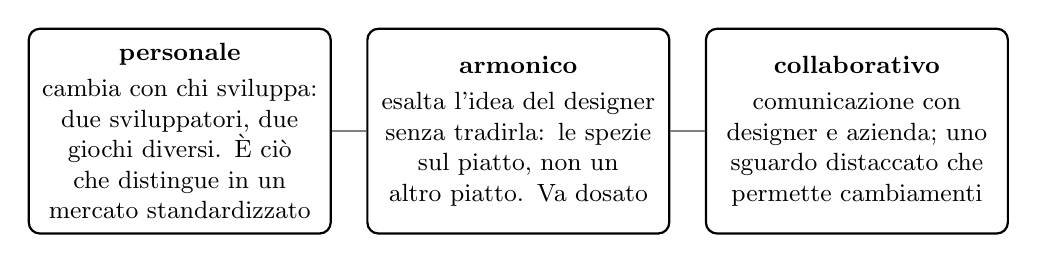
\begin{tikzpicture}[
  font=\small,
  a13pr/.style={draw, thick, rounded corners=4pt, text width=3.6cm, align=center,
                minimum height=2.6cm, fill=white},
]
  \node[a13pr] (p1) at (0,0) {\textbf{personale}\\[2pt]cambia con chi sviluppa: due
    sviluppatori, due giochi diversi. È ciò che distingue in un mercato
    standardizzato};
  \node[a13pr] (p2) at (4.3,0) {\textbf{armonico}\\[2pt]esalta l'idea del designer senza
    tradirla: le spezie sul piatto, non un altro piatto. Va dosato};
  \node[a13pr] (p3) at (8.6,0) {\textbf{collaborativo}\\[2pt]comunicazione con designer
    e azienda; uno sguardo distaccato che permette cambiamenti};
  \draw[thick, gray] (p1) -- (p2) -- (p3);
\end{tikzpicture}
\caption{I tre principi dello sviluppo secondo Marta.}
\label{a13:fig:principi}
\end{figure}

% ---------------------------------------------------------------------
\section{Gli \emph{stakeholder}: chi ha voce sul gioco}
\label{a13:sec:stakeholder}

\slidefig{img/AGD/agd13-stakeholder}{Gli stakeholder.}{slide \emph{Sviluppo di giochi}}{fig:agd13-stakeholder}


Chi sono, più nel dettaglio, gli \emph{stakeholder} tra cui lo sviluppo media? I primi
due sono già emersi: \textbf{il designer} (o la designer) e \textbf{la casa editrice}. Ma
una parte che ``molto spesso viene trascurata e tralasciata'' è \textbf{chi poi gioca il
gioco}: i clienti, le clienti. Quando si fa un gioco è importante ricordarsi \textbf{per
chi lo si sta facendo}, e quella è proprio la voce che non si sente: in una riunione
sul gioco c'è la casa editrice, nella veste del direttore editoriale, c'è l'autore o
l'autrice, ma \textbf{non c'è chi poi lo compra e lo gioca}, ``perché non si può''. Al
massimo si prendono dei \emph{playtester}, ma è una visione parziale; oppure, con un po'
di esperienza del mercato e delle persone a cui il gioco arriva, si può \textbf{fare le
veci di quella parte}. Marta lo fa spesso: ``sì, ma questa modifica va nell'interesse di
chi compra il gioco? Magari è una cosa che piace a noi qua dentro, ma a chi lo compra non
interessa''.

Non è detto che le tre parti ci siano sempre: quando c'è una casa editrice è probabile
che ci sia anche un cliente, ma possono mancare altre parti, o essercene altre ancora.
Se il gioco è \textbf{su licenza}, uno \emph{stakeholder} è \textbf{chi ha fornito la
licenza}, che ha i suoi vincoli e i suoi paletti. Può esserci una persona che ha
\textbf{scritto il \emph{world building}} del gioco e vuole che venga mantenuto in un
certo modo. ``Anche qua potrebbero esserci molte più variabili di quelle che viene da
pensare in prima battuta.''

\begin{figure}[htbp]
\centering
\begin{tikzpicture}[
  font=\small,
  a13st/.style={draw, thick, rounded corners=4pt, text width=2.7cm, align=center,
                minimum height=1.1cm, fill=white},
  a13opt/.style={draw, thick, dashed, rounded corners=4pt, text width=2.7cm, align=center,
                 minimum height=1.1cm, fill=white},
  a13arr/.style={{Stealth[length=2.5mm]}-{Stealth[length=2.5mm]}, thick}
]
  \node[draw, very thick, circle, fill=gray!15, minimum size=2.4cm, align=center] (sv)
    at (0,0) {\textbf{sviluppo}\\(mediazione)};
  \node[a13st] (des) at (-4.2,1.6) {\textbf{designer}\\la visione originale};
  \node[a13st] (pub) at (4.2,1.6) {\textbf{casa editrice}\\catalogo, mercato,
    reparti};
  \node[a13st, fill=gray!8] (cli) at (0,-2.9) {\textbf{chi gioca}\\(la voce che non c'è
    alle riunioni)};
  \node[a13opt] (lic) at (-4.2,-1.6) {chi ha dato la \textbf{licenza}};
  \node[a13opt] (wb) at (4.2,-1.6) {chi ha scritto il \textbf{\emph{world building}}};
  \foreach \n in {des,pub,cli}{\draw[a13arr] (sv) -- (\n);}
  \foreach \n in {lic,wb}{\draw[a13arr, dashed] (sv) -- (\n);}
\end{tikzpicture}
\caption{Gli \emph{stakeholder} di un gioco secondo la lezione. In tratteggio quelli che
ci sono solo in alcuni progetti. La voce di chi gioca arriva solo attraverso i
\emph{playtest} o attraverso chi sviluppa, che con l'esperienza ne fa le veci.}
\label{a13:fig:stakeholder}
\end{figure}

\paragraph{Approfondimento: partecipanti e ``avvocati''.} Bateman e Boon, in \emph{21st
Century Game Design}, aprono il libro con un principio che chiamano \emph{Zen Game
Design}: ``il game design deve essere privo di ego, bilanciando i desideri e i bisogni di
tutti i partecipanti''. I \emph{partecipanti} sono chiunque abbia un interesse nel
progetto (il pubblico, l'editore, lo studio, i programmatori, gli artisti, il marketing,
e, ``sempre più spesso'', il \emph{detentore della licenza}); poiché non tutti possono
partecipare al \emph{design}, alcune figure fanno da \emph{advocate}, da portavoce, per
gli altri. Gli autori notano proprio ciò che nota Marta: per il pubblico, di solito,
\emph{non c'è} un portavoce formale, e il compito ricade su chi progetta; e a proposito
della licenza consigliano di tenere aperto il dialogo durante tutto lo sviluppo, invece di
mostrare il gioco finito al licenziatario ed essere costretti a cambiarlo quando i
cambiamenti costano di più. Il libro parla di videogiochi, e di \emph{designer} più che
di sviluppatori, ma la figura che Marta descrive (chi si fa carico delle voci assenti)
corrisponde quasi esattamente al loro \emph{advocate}.

% ---------------------------------------------------------------------
\section{\emph{Design} contro sviluppo}
\label{a13:sec:designvs}

\slidefig{img/AGD/agd13-design}{Design e sviluppo a confronto.}{slide \emph{Sviluppo di giochi}}{fig:agd13-design}


Qui arriva, dice Marta, ``la differenza più sostanziale'' tra \emph{design} e sviluppo.
Avverte subito che è una visione ``un po' stereotipica'': non è detto che chi fa
\emph{design} abbia tutte queste caratteristiche, né chi fa sviluppo tutte le altre; ma
è ``una buona cartina di tornasole'' per distinguere le due figure. Il confronto è
riassunto nella tabella~\ref{a13:tab:designvs}.

\paragraph{Chi fa \emph{design}.}
\begin{itemize}
  \item \textbf{Non è \emph{time driven}}: normalmente non ha una scadenza vera e propria.
        Può pensare a una scadenza nel senso di ``questo \emph{design} tra cinque anni non
        è più interessante'', ma di base non ha ristrettezze temporali. Diverso è il caso di
        un \emph{design} su commissione.
  \item Ha \textbf{piena libertà creativa}: può muoversi liberamente, presentare qualsiasi
        idea e cercare il canale giusto per pubblicarla, senza vincoli.
  \item Ha di solito un \textbf{attaccamento emotivo}: il gioco l'ha creato, c'è qualcosa
        di suo. È positivo, perché permette di mettere nel gioco caratteristiche che una
        persona senza quell'amore per il progetto non metterebbe; ed è negativo, perché
        rende difficile fare modifiche, e a volte stravolgimenti, ``perché magari ci si è
        affezionati''.
  \item Ha l'\textbf{originalità}: si può prendere qualsiasi cosa e metterla dentro.
        ``Vado a prendere dei cubetti d'oro, di oro vero, e li metto nel gioco'':
        chi fa \emph{design} potrebbe volerlo fare, e il \emph{design} non lo impedisce; il
        problema, semmai, sarà della casa editrice. Ed è proprio lì che vengono fuori le
        cose ``un po' rivoluzionarie'' che a volte servono per smuovere i mercati, per
        alzare l'asticella.
  \item Ha \textbf{un'idea}: l'idea di partenza è ciò che caratterizza il \emph{design}.
        Non deve essere ``fatta e finita'', né completamente bilanciata, né
        completamente finalizzata: deve far capire le intenzioni. Negli anni c'è stata una
        \textbf{professionalizzazione del \emph{design}}, e oggi i designer portano in
        genere il progetto molto più avanti che in passato; ma resta la possibilità di
        dichiarare chiusa un'idea in qualsiasi momento (``questo è sufficiente per far
        capire che cosa dovrebbe essere sviluppato'') e consegnarla a una casa editrice.
\end{itemize}

\paragraph{Chi fa sviluppo.}
\begin{itemize}
  \item Ha \textbf{scadenze}: il \textbf{\emph{time to market}}, cioè quando il gioco deve
        uscire per prendere la spinta giusta del mercato, e il \textbf{vincolo del
        contratto} firmato tra casa editrice (o chi sviluppa) e designer. A un certo punto
        il gioco deve uscire, essere finalizzato, completato.
  \item Ha \textbf{restrizioni produttive}: tornando ai cubetti d'oro, ``io poi devo fare i
        conti con la realtà di mettere dei cubetti d'oro su mille scatole''. Come si fa?
        Sono veramente necessari? Sono veramente la cosa che serve?
  \item Esercita il \textbf{distacco}: non avendo un legame emotivo con il progetto,
        soprattutto all'inizio, può analizzarlo in modo più freddo e riconoscere quali
        caratteristiche servono all'idea per funzionare sul mercato, per certi clienti.
  \item Porta la \textbf{standardizzazione}, che ha due facce. È positiva perché un'idea
        troppo originale può spaventare alcune fette di mercato: un gioco molto originale
        viene recepito ``in modo misto, se va bene'', spesso male, perché il mercato ``non
        è pronto'', non aveva in mente quel gioco. La standardizzazione \textbf{smussa gli
        angoli}, rende il gioco più digeribile, più simile ad altre cose. Ma smussare gli
        angoli rischia anche di \textbf{portare via le caratteristiche importanti} del
        gioco.
  \item Ha l'\textbf{esperienza}\footnote{In questo punto la trascrizione è coperta da
        alcune righe di frasi ripetute senza senso (``è falsata da un pubblico''); la
        quinta voce della slide si ricostruisce dal discorso che segue e dalla sezione
        successiva, dedicata proprio all'esperienza.}: un designer che ha fatto un solo
        gioco ha ``pochissima'' esperienza, mentre chi fa sviluppo ha in genere lavorato a
        più titoli, perché si muove più rapidamente tra più progetti. Sa già dire ``questa
        cosa su itch.io non funziona, perché se lo pubblichi così le persone non capiscono
        neanche che tipo di gioco è: perché non evidenziamo questi aspetti?''. Un prodotto
        sullo scaffale, o caricato su itch.io, funziona?
\end{itemize}

\begin{table}[htbp]
\centering
\small
\begin{tabular}{@{}p{3.0cm}p{5.0cm}p{5.4cm}@{}}
\toprule
 & \textbf{Chi fa \emph{design}} & \textbf{Chi fa sviluppo} \\
\midrule
Tempo & non \emph{time driven} (salvo commissione) & scadenze: \emph{time to market},
  contratto \\
Libertà & piena libertà creativa & restrizioni produttive (i ``cubetti d'oro'' su mille
  scatole) \\
Rapporto col gioco & attaccamento emotivo (pro e contro) & distacco, analisi ``fredda'' \\
Direzione & originalità, anche rivoluzionaria & standardizzazione: smussa gli angoli
  (pro e contro) \\
Che cosa porta & un'idea, anche non finita & esperienza su molti titoli e generi \\
\bottomrule
\end{tabular}
\caption{\emph{Design} contro sviluppo secondo la slide di Marta: una visione volutamente
``stereotipica'', utile come cartina di tornasole. Nella realtà i confini sono sfumati.}
\label{a13:tab:designvs}
\end{table}

\paragraph{Confini sfumati.} Che cosa succede se un'idea è \textbf{troppo embrionale}? O se
un'implementazione che si va a fare \textbf{cambia l'esperienza di gioco}? ``Queste sono
domande importantissime, dove le cose si sfumano.'' A volte si ricevono idee così
embrionali che quasi non converrebbe prenderle, perché c'è così tanto sviluppo da fare
che non si sa più quanto è sviluppo e quanto è \emph{design}. Dall'altra parte c'è il
rischio che fare sviluppo \textbf{comprometta l'esperienza originale}. Questi ruoli vanno
immaginati come ``qualcosa di molto permeabile'', e non è mai facile mettere l'asticella
nel punto giusto: ``io molto spesso me lo chiedo: ma per questo gioco ho fatto
effettivamente sviluppo? Sono arrivata addirittura a fare \emph{design}?''. Con
l'esperienza diventa più facile tracciare la linea: capire se l'idea è davvero troppo
embrionale, e quindi non conviene svilupparla, o se c'è stato un eccesso (``ho fatto
troppo sviluppo, ho cambiato l'idea di partenza'') e bisogna tornare sui propri passi e
far emergere di più l'idea originale del designer.

% ---------------------------------------------------------------------
\section{Lo sviluppo è esperienziale}
\label{a13:sec:esperienza}

Marta lo ha detto più volte: lo sviluppo \textbf{si fonda sull'esperienza}. Da qualche
parte si parte, ``ci si improvvisa un po', come in tutte le cose'', ma poi l'esperienza si
accumula e fa la differenza. Non c'è un modo esatto di accumularla, ma c'è una differenza
di fondo tra le due figure.

\paragraph{Il designer focalizzato.} Chi fa \emph{design} può fare continuamente lo stesso
\emph{design}, senza esplorare tanti giochi e tante idee diverse. L'esempio è \textbf{Uwe
Rosenberg}\footnote{Nella trascrizione solo ``Rosenberg''; dal contesto (piazzamento
lavoratori, piazzamento tessere) è quasi certamente Uwe Rosenberg, l'autore di
\emph{Agricola}, citato più avanti nella lezione.}, che ha ``tre o quattro temi'' e tende
a fare giochi su quelli: il piazzamento lavoratori, il piazzamento tessere, e poi qualche
esperimento su altri generi. Una visione non ristretta in senso negativo, precisa Marta:
``\textbf{focalizzata} è il termine giusto''. Una visione che, nella sua iteratività, lo ha
portato a raggiungere \textbf{l'apice dei generi} in cui ha lavorato, perché li ha
``talmente tanto sviscerati'' da conoscerne forze e debolezze.

\paragraph{Lo sviluppatore che tocca tutto.} Chi sviluppa, al contrario, entra in contatto
con \textbf{tantissimi generi diversi}, perché le idee non vengono sempre dalla stessa
persona. Marta ha sviluppato giochi che durano più di due ore, giochi leggeri,
\emph{party game}, giochi di destrezza astratti: ``si tocca un po' tutto quello che
esiste''. Vale anche per il gioco di ruolo, dove chi sviluppa può muoversi più facilmente
tra sistemi diversi, dal gioco di una pagina (\emph{one page}) al manuale di 50 pagine con
campagna.

% ---------------------------------------------------------------------
\section{Il rapporto tra chi progetta e chi sviluppa}
\label{a13:sec:rapporto}

\slidefig{img/AGD/agd13-rapporto}{Il rapporto tra designer e developer.}{slide \emph{Sviluppo di giochi}}{fig:agd13-rapporto}


L'esperienza passa anche attraverso il \textbf{rapporto tra designer e \emph{developer}},
che ``deve essere saputo gestire'': per le differenze appena viste, per i livelli diversi
di esperienza, per i ruoli diversi, che a volte sembrano perfino contrapposti. Ma è, come
detto all'inizio, un rapporto di mediazione, e la cosa importante è \textbf{trovare i
compromessi}. Ogni rapporto è diverso: non si lavora con tutti i designer nello stesso
modo.

\paragraph{Collaborazione attiva e passiva.} A Marta sono capitate entrambe.
\begin{itemize}
  \item Una \textbf{collaborazione attiva} è uno \textbf{scambio ricorrente} tra le due
        parti: ci si aggiorna a vicenda, si fanno cambiamenti, ``ci si rimbalzano molto le
        idee e il progetto''.
  \item Una \textbf{collaborazione passiva} è quando una delle due parti prende in carico
        la maggior parte del lavoro e \textbf{riceve dei \emph{feedback}} dall'altra, e il
        rapporto si limita a questo. Può capitare, per esempio, che un gioco venga
        valutato, firmato con la casa editrice, e che poi chi l'ha progettato
        ``praticamente sparisca''. \textbf{È legittimo}: l'idea è stata fornita, i dubbi, se
        c'erano, si spera siano stati risolti, e magari il designer non ha interesse a
        vedere come si sviluppa il gioco da lì in poi, e vuole vederlo solo a cose fatte.
\end{itemize}

\paragraph{Le aspettative.} È importante anche \textbf{gestire le aspettative}: ricordarsi
che quando un gioco passa per altre persone \textbf{viene inevitabilmente modificato}.
``Un gioco è un processo di collaborazione'': non c'è una sola persona che lo fa. La
figura del designer è stata più volte messa in primo piano, ma il processo è
\textbf{collettivo}: il gioco non arriverebbe sullo scaffale senza chi lo produce, chi fa
la grafica e le illustrazioni, e chi lo sviluppa. Affidando un gioco a una casa editrice
o a chi sviluppa, il gioco \textbf{cambierà}, anche in modi che non sempre troveranno
d'accordo. L'importante è trovare i compromessi giusti.

\paragraph{La fiducia.} E qui viene l'ultimo punto: la \textbf{fiducia}. ``Come se si
vogliono avere delle relazioni nella vita'', bisogna avere una fiducia reciproca. Il
consiglio di Marta, anche ai designer: \textbf{cercatevi case editrici, sviluppatori o
sviluppatrici con cui pensate che possa esserci un buon rapporto di fiducia}, perché i
rapporti vanno male soprattutto quando questa fiducia viene a mancare, quando una delle
due parti pensa che l'altra ``non stia facendo gli interessi del gioco''.

% ---------------------------------------------------------------------
\section{Da dove viene il ruolo: \emph{developer} ed \emph{editor}}
\label{a13:sec:storia}

\slidefig{img/AGD/agd13-storia}{Brevi cenni storici sullo sviluppo.}{slide \emph{Sviluppo di giochi}}{fig:agd13-storia}


``Vi siete chiesti chi è l'\emph{editor}, in questo calderone?'' Per rispondere Marta
racconta da dove nasce la figura dello sviluppo.

\paragraph{Gli anni Settanta e i \emph{wargame}.} Siamo negli anni '70, e la
\textbf{SPI}, \emph{Simulations Publications, Inc.}\footnote{Marta dice ``Simulation
Publishing Inc., credo''; il nome corretto della casa editrice americana di
\emph{wargame} è \emph{Simulations Publications, Inc.}}, una casa editrice americana di
\emph{wargame}, ha bisogno di pubblicare \textbf{più \emph{wargame}}: chi fa \emph{design}
``non ce la fa a fare tutti questi''. A questo punto la trascrizione si interrompe per
alcune frasi ripetute senza senso, e una parte del racconto va perduta\footnote{Coprono
la spiegazione di come la SPI risolse il problema. Il capitolo non la ricostruisce; si
sa, in generale, che nella SPI il \emph{developer} era la figura che riceveva il
\emph{design} e lo portava a un gioco pubblicabile, ma la trascrizione non permette di
dire che cosa abbia detto Marta.}. Quando il discorso riprende, Marta sta elencando le
case editrici che, dopo, hanno deciso di \textbf{inserire degli sviluppatori}:
\textbf{Fantasy Flight}, la linea \textbf{\emph{alea}} di Ravensburger e \textbf{Hans im
Glück}\footnote{Nella trascrizione ``la linea Alia di Ravensburger'' e ``Huntington
Gluck'', poi ``Hansingluck''.}. Gli sviluppatori sono ``fondamentalmente delle figure che
fanno le veci dei designer all'interno delle aziende'', ma \textbf{non sono designer in
senso stretto}: avranno idee e visioni diverse, ed è qui che nasce il rapporto
collaborativo come lo conosciamo oggi.

\paragraph{L'\emph{editor} tedesco.} Contemporaneamente c'era un'altra figura,
l'\textbf{\emph{editor}}, molto diffusa in \textbf{Germania}: era la persona che si
occupava di \textbf{portare il gioco a compimento}. Le altre case editrici tedesche avevano
un \emph{editor}, e lo avevano anche \emph{alea} e Hans im Glück; ma l'\emph{editor}
\textbf{non si occupava del gioco nell'aspetto meccanico e regolistico}: si occupava di
tutti gli altri aspetti.

\paragraph{L'inversione.} Andando avanti le due figure \textbf{si sono ibridate}, e oggi si
sono ``un po' invertite'': lo \textbf{sviluppo}, che prima si occupava solo della parte
meccanica, oggi prende in carico \textbf{tutti gli aspetti}, compresa la parte meccanica;
l'\textbf{\emph{editor}} ha un ruolo più piccolo, legato soprattutto \textbf{alle parole}:
rivede i testi, controlla che siano in italiano corretto, si accerta che tutto sia
presentato al meglio. Questa è, oggi, la figura che di solito si chiama \emph{editor} nel
gioco da tavolo. Ma non è definito in modo assoluto: ci sono case editrici che chiamano
``sviluppatore'' chi fa \emph{editing}, e case che fanno \emph{editing} e non hanno
sviluppatori. È una figura nata negli ultimi anni e \textbf{non c'è ancora una
standardizzazione}; questa, confrontandosi con colleghi e colleghe di altre aziende, è la
tendenza che Marta vede.

\begin{figure}[htbp]
\centering
\begin{tikzpicture}[
  font=\small,
  a13ev/.style={draw, thick, rounded corners=3pt, text width=3.5cm, align=center,
                minimum height=1.4cm, fill=white},
  a13arr/.style={-{Stealth[length=3mm]}, thick}
]
  \draw[a13arr] (0,0) -- (13.4,0);
  \foreach \x/\lab in {1.6/anni '70, 6.4/poi, 11.4/oggi}{
    \fill (\x,0) circle (2.5pt);
    \node[below=4pt, font=\footnotesize] at (\x,0) {\lab};
  }
  % sopra: developer
  \node[a13ev, above=0.5cm] at (1.6,0) {SPI (\emph{wargame}): servono più giochi di quanti
    i designer riescano a farne};
  \node[a13ev, above=0.5cm] at (6.4,0) {Fantasy Flight, \emph{alea} (Ravensburger), Hans
    im Glück inseriscono gli \textbf{sviluppatori}: parte meccanica};
  \node[a13ev, above=0.5cm, fill=gray!12] at (11.4,0) {\textbf{sviluppo}: tutti gli
    aspetti, meccanica compresa};
  % sotto: editor
  \node[a13ev, below=0.7cm] at (6.4,0) {l'\textbf{\emph{editor}} (soprattutto in Germania)
    porta il gioco a compimento, \emph{tranne} meccanica e regole};
  \node[a13ev, below=0.7cm, fill=gray!12] at (11.4,0) {\textbf{\emph{editor}}: le parole,
    i testi, la presentazione};
  \node[font=\footnotesize\itshape, rotate=90] at (-0.4,1.4) {\emph{developer}};
  \node[font=\footnotesize\itshape, rotate=90] at (-0.4,-1.5) {\emph{editor}};
\end{tikzpicture}
\caption{Come Marta racconta la nascita delle due figure e la loro ``inversione''. Le
date intermedie non sono dette, e una parte del racconto è persa nella trascrizione. Oggi
le definizioni non sono ancora standardizzate.}
\label{a13:fig:storia}
\end{figure}

\paragraph{Prima pausa.} ``Siamo alla seconda parte'': Marta propone una pausa di una
decina di minuti e invita a portare domande al ritorno. Durante la pausa la trascrizione
registra il commento su un videogioco di cui si è detto nelle avvertenze, e poi diversi
minuti di frasi ripetute in ciclo. Quando si riprende, uno studente avverte che sta
ancora mangiando, ``ma ci sono, nessun problema''. Marta chiede se ci sono domande o
curiosità (``non so se vi posso rispondere in pieno, perché c'è una parte di segreto
professionale, ma possiamo ingegnarci'').

% ---------------------------------------------------------------------
\section{Il conflitto di interessi}
\label{a13:sec:conflitto}

La prima domanda è di \textbf{Gianmarco}\footnote{Più avanti Marta si riferisce a questa
domanda come ``quella domanda che ha fatto Gianmarco''.}, ``fra la curiosità e la
provocazione'': lo sviluppatore, di solito, è \textbf{assunto dalla casa editrice}, mentre
il designer non lo è necessariamente. \textbf{Non c'è un conflitto di interessi} nel fare
da mediatore tra due parti, quando si è assunti da una delle due? ``È un'ottima domanda,
onestamente'', risponde Marta, ``non so neanche se riuscirò a soddisfarti''.

\paragraph{Com'era prima.} All'inizio la figura non c'era, e il rapporto era diverso: i
designer avevano un gioco e la casa editrice si limitava a \textbf{metterlo sul mercato
così com'era stato pensato}; rivedeva i testi, curava la produzione fisica. ``Addirittura
i designer brevettavano i tabelloni'': erano tempi diversi. Funzionava quando \textbf{il
mercato era piccolo}, le idee erano poche e c'era tantissimo spazio per presentarle.

\paragraph{Com'è oggi.} Oggi a \textbf{Essen}, la più grande fiera al mondo di giochi da
tavolo, secondo le ultime stime che Marta ricorda si parla di qualcosa come \textbf{2500
nuovi giochi presentati in un solo anno}, e solo tra quelli pubblicati in qualche forma,
senza contare tutta la realtà indipendente che pubblica su itch.io e simili. ``Il volume
di giochi presentati ogni anno è spaventoso.'' Le case editrici, molto spesso,
\textbf{non possono permettersi di sbagliare un titolo} (``cannare'', dice Marta): dipende
dalle dimensioni, ma una piccola casa editrice che sbaglia anche solo un paio di titoli
può chiudere, perché \textbf{l'investimento nel gioco analogico è importante}. Per questo la
cosa fondamentale è che il gioco \textbf{rispetti le aspettative di mercato}. E chi fa
\emph{design} non è tenuto a conoscerle, e probabilmente non ha i mezzi per farlo: Marta
non conosce ``tantissime designer'' che abbiano la possibilità di andare a Essen e
interfacciarsi con più editori, anche internazionali. È un limite, e oggi \textbf{avere
dentro l'azienda una figura che fa le tue veci} per tutte queste questioni è generalmente
visto come positivo, anche se non vale per tutte le persone.

\paragraph{Che cosa fa Marta.} Marta sconsiglia spesso di fare giochi \textbf{solo con
l'obiettivo di pubblicare con una casa editrice}: capisce che i soldi facciano gola, ma
bisogna saper riconoscere \textbf{quali giochi sono adatti al mercato}, trovare la casa
editrice che fa per noi e vedere se con le persone con cui si collabora ci si trova bene.
Lei, da parte sua, cerca di \textbf{rispettare le volontà del designer}, proprio perché sa
di essere assunta dalla casa editrice, ma anche di essere, in quel momento,
\textbf{l'unica persona che sta parlando per il designer}, che magari non c'è a tutte le
riunioni: diventa importante difendere le sue idee. Si rende conto che non è sempre
facile, e che non è facile nemmeno accettare la dinamica. ``In un mondo ideale'' chi fa
\emph{design} potrebbe partecipare attivamente alle quaranta ore lavorative in azienda in
cui si fanno le cose; nella realtà le dinamiche sono complesse. Gianmarco si dice
soddisfatto: ``mi è abbastanza chiara la risposta''.

\paragraph{Approfondimento: il portavoce assunto.} La domanda di Gianmarco è la stessa che
Bateman e Boon si pongono a proposito del produttore esterno, il portavoce dell'editore
nei progetti di videogiochi: secondo loro molti sviluppatori ne risentono
l'``interferenza'', ma il problema nasce di solito quando il portavoce cerca di
\emph{prendersi il controllo} del \emph{design}, invece di rappresentare i bisogni di chi
rappresenta. La risposta di Marta sposta il problema nello stesso punto: il ruolo regge
finché chi sviluppa si comporta da mediatore, e dà voce anche a chi, in quella stanza, non
c'è.

% ---------------------------------------------------------------------
\section{Le otto fasi dello sviluppo}
\label{a13:sec:fasi}

\slidefig{img/AGD/agd13-fasi}{Le otto fasi dello sviluppo.}{slide \emph{Sviluppo di giochi}}{fig:agd13-fasi}


Oggi, ripete Marta, si fa un'infarinatura generale; la prossima volta qualche esempio più
pratico e qualche tecnica. ``La realtà della faccenda è che \textbf{non c'è un modo esatto
di procedere}'': ogni gioco fa storia a sé, e non si sviluppa un gioco totalmente
narrativo come si sviluppa un gioco di destrezza. Raccomanda di \textbf{pensare in modo
elastico}, perché è facile farsi ingannare e pensare che le cose siano lineari: ``non è mai
così''. Ed è anche l'aspetto bello del lavoro: c'è sempre una sfida nuova. ``Io mi sono
improvvisamente scoperta appassionata di bonsai soltanto perché ho lavorato a un gioco che
parlava di bonsai'': se si è persone curiose, ``è un bel lavoro''.

Marta ha riassunto il lavoro in \textbf{otto fasi} (figura~\ref{a13:fig:fasi}):
\textbf{selezione}, \textbf{ricerca}, \textbf{concettualizzazione},
\textbf{presentazione}, \textbf{\emph{testing}}, \textbf{implementazione},
\textbf{preparazione degli \emph{asset}}, \textbf{revisioni}. È, grosso modo, la
\emph{pipeline} di un gioco dal primo momento in cui viene accettato nel ramo di sviluppo
di un'azienda a quando lascia l'azienda per essere stampato e finire sullo scaffale. Le
fasi \textbf{non si svolgono necessariamente in quest'ordine}: a volte si torna indietro, a
volte mancano dei pezzi; c'è tanto scambio e tanto dialogo con tutti i reparti per
arrivare alla fine ``nel modo più celere possibile'', ma ``molto spesso arrivano i
disastri e bisogna tornare indietro''. In questa lezione Marta arriva fino alla
preparazione degli \emph{asset}; le \textbf{revisioni} e il \textbf{come scrivere un
regolamento} restano per venerdì (sezione~\ref{a13:sec:chiusura}).

\begin{figure}[htbp]
\centering
\begin{tikzpicture}[
  font=\small,
  a13ph/.style={draw, thick, rounded corners=3pt, text width=2.3cm, align=center,
                minimum height=1.0cm, fill=white},
  a13arr/.style={-{Stealth[length=2.5mm]}, thick}
]
  \node[a13ph] (f1) at (0,1.6) {1.\ selezione};
  \node[a13ph] (f2) at (3.1,1.6) {2.\ ricerca};
  \node[a13ph] (f3) at (6.2,1.6) {3.\ concettua-\\lizzazione};
  \node[a13ph] (f4) at (9.3,1.6) {4.\ presentazione};
  \node[a13ph] (f5) at (9.3,-0.6) {5.\ \emph{testing}};
  \node[a13ph] (f6) at (6.2,-0.6) {6.\ implementa-\\zione};
  \node[a13ph] (f7) at (3.1,-0.6) {7.\ preparazione\\degli \emph{asset}};
  \node[a13ph, fill=gray!12] (f8) at (0,-0.6) {8.\ revisioni\\(venerdì)};
  \draw[a13arr] (f1) -- (f2);
  \draw[a13arr] (f2) -- (f3);
  \draw[a13arr] (f3) -- (f4);
  \draw[a13arr] (f4) -- (f5);
  \draw[a13arr] (f5) -- (f6);
  \draw[a13arr] (f6) -- (f7);
  \draw[a13arr] (f7) -- (f8);
  \draw[a13arr, dashed] (f2.north) to[bend right=35] node[above, font=\footnotesize]
    {si torna indietro} (f1.north);
  \draw[a13arr, dashed] (f6.south) to[bend right=40] node[below, font=\footnotesize]
    {ogni ciclo di \emph{test}} (f5.south);
  \draw[a13arr, dashed] (f5.south west) to[bend left=25] (f6.south east);
  \node[font=\footnotesize, text width=4.2cm, align=left, anchor=west] at (-1.2,-2.9)
    {\emph{ingresso}: un prototipo accettato};
  \node[font=\footnotesize, text width=4.2cm, align=right, anchor=east] at (10.5,-2.9)
    {\emph{uscita}: il gioco va in stampa};
\end{tikzpicture}
\caption{Le otto fasi dello sviluppo secondo Marta. L'ordine è indicativo: le frecce
tratteggiate ricordano che si torna spesso indietro (per esempio la ricerca informa la
selezione, e implementazione e \emph{testing} si alternano in ciclo).}
\label{a13:fig:fasi}
\end{figure}

% ---------------------------------------------------------------------
\section{La selezione}
\label{a13:sec:selezione}

\slidefig{img/AGD/agd13-selezione}{La selezione.}{slide \emph{Sviluppo di giochi}}{fig:agd13-selezione}


La selezione comincia quando si riceve un \textbf{prototipo}, e se ne ricevono
\textbf{tantissimi}. Marta non sa fare una stima precisa, perché cambia molto da periodo a
periodo e da casa editrice a casa editrice; ma nell'ultimo mese, se non sbaglia, a dV
Giochi ne sono arrivati \textbf{una sessantina}. dV è una casa editrice grande, e altre ne
ricevono meno; ma si immagini di dover valutare 60 prototipi al mese: ci deve essere
\textbf{una cernita}, e avviene in vari modi.

\begin{itemize}
  \item \textbf{Catalogo e mercato di riferimento.} C'è una scrematura iniziale legata al
        catalogo. dV Giochi non pubblica giochi che superano i \textbf{45 minuti, un'ora}:
        se arriva un gioco che dura due ore e mezza, probabilmente viene scartato a
        priori, perché è molto improbabile che faccia al caso loro. Un'occhiata si dà
        sempre, però: magari c'è un'idea buona, magari le due ore e mezza sono una stima
        sbagliata dell'autore.
  \item \textbf{La complessità.} Un buon gioco può risultare \textbf{eccessivamente
        complesso}, nel senso che è difficile da spiegare e da far capire, e allora non ci
        sono i margini per provarlo e testarlo adeguatamente: ``magari devo studiarmi un
        regolamento per quattro giorni, e io quattro giorni da passare a provare un gioco
        non ce li ho''. Va valutato: è un gioco che si può testare con il designer? Fa
        davvero al caso nostro?
  \item \textbf{La sensibilità del \emph{team} editoriale.} Lo sviluppo è personale, e
        questo si riflette in tutto: ``se non ci piacciono i giochi in tempo reale, è
        inutile che pensiamo che quel gioco in tempo reale funzioni benissimo'', perché se
        poi non riusciamo a metterci a svilupparlo stiamo solo perdendo tempo. In ambito
        professionale non contano solo le preferenze (``altrimenti io svilupperei solamente
        due tipi di giochi''), ma ci sono giochi che si sa che non funzioneranno con quel
        \emph{team}. Marta, per esempio, ``non è ferratissima'' sui \textbf{giochi di
        destrezza}: tende a evitarli o a passarli a un collega (``tu che hai più la
        sensibilità per questa cosa, ci vedi qualcosa in questo gioco?''), perché anche
        fisicamente fa fatica a valutarli. Una casa editrice brava riesce a riflettere
        queste sensibilità nel suo catalogo. E bisogna tenerle a mente perché i giochi
        selezionati vanno poi testati, provati, discussi con i designer: ``quello che inizia
        come un processo di un'ora, un'ora e mezzo potrebbe diventare tranquillamente di
        giorni''.
  \item \textbf{La coerenza sull'asse tema--meccaniche.} Negli ultimi anni ci sono
        tantissimi giochi che si assomigliano. Una volta si tendeva a privilegiare uno dei
        due aspetti, di solito le meccaniche, e poi c'era il cosiddetto \textbf{\emph{window
        dressing}}: si ``appiccicava'' sopra un tema che giustificasse un po' le
        meccaniche. Negli anni questo ha portato a una \textbf{stagnazione}, e oggi c'è
        anche ``un po' di pesantezza'' da questo punto di vista. Oggi è molto importante che
        \textbf{meccaniche e tema si parlino in modo molto stretto}. Questo significa che il
        gioco si può modificare di meno, e che c'è più rischio che non venga accettato:
        ``lato designer è un incubo'', perché si lavora a un gioco per tantissimo tempo e
        poi non viene accettato perché non piace il tema, e se il legame è forte non si
        può più dire ``cambia il tema, qual è il problema?''. Ma è anche ciò che oggi fa
        scegliere un gioco sopra gli altri. L'esempio è \textbf{\emph{Hegemony}}\footnote{Nella
        trascrizione ``Egemoni''; si tratta con ogni probabilità di \emph{Hegemony: Lead
        Your Class to Victory}, un gioco gestionale sulle classi sociali e sulla politica
        economica di uno Stato.}, un gioco gestionale (``vedo un sì'', dice Marta quando
        chiede se la classe lo conosce) che ricrea le dinamiche della politica di uno Stato
        ``in modo molto viscerale'': è una simulazione astratta, ma i designer hanno legato
        le meccaniche al tema ``in modo indissolubile''. Non si può prendere \emph{Hegemony}
        e farne un gioco sugli esploratori di \emph{dungeon}, ``perché non regge''; mentre su
        un gioco di carte con solo numeri si può mettere il \emph{dungeon}, o un tema
        diverso, perfino politico.
\end{itemize}
Sono criteri generici, ``che ci aiutano a selezionare i giochi più promettenti'', a capire
quali meritano una possibilità di sviluppo.

% ---------------------------------------------------------------------
\section{La ricerca}
\label{a13:sec:ricerca}

\slidefig{img/AGD/agd13-ricerca}{La ricerca.}{slide \emph{Sviluppo di giochi}}{fig:agd13-ricerca}


Dopo la selezione c'è la \textbf{ricerca}. Lo strumento principale, nel mondo del gioco da
tavolo, è \textbf{BoardGameGeek} (BGG): è ``il sito di riferimento'' perché è un
\textbf{\emph{database}}, ed è lo strumento più usato nell'industria, ``con tutti i limiti
che ha'': è una visione \textbf{americano-centrica}, perché la sua utenza è prevalentemente
quella. Ma resta indispensabile, perché vi si trovano tantissime informazioni.

\paragraph{Le domande della ricerca.} Si immagini di aver appena visto, e accettato, il
prototipo di \emph{Hegemony}: un gioco sulla politica e sugli Stati. Prima di tutto
bisogna capire:
\begin{itemize}
  \item ce ne sono altri sul mercato che fanno già la stessa cosa?
  \item se sì, che cosa fanno di diverso?
  \item quali caratteristiche li esaltano, o li affossano?
  \item come sono percepiti dalle persone?
  \item che cosa si può fare di diverso? Magari l'idea è valida, ma approfondendo si scopre
        che ci sono tanti giochi sulla politica di uno Stato: che cosa fa di diverso
        questo?
\end{itemize}
Si conoscono così i temi comuni: andando su BGG e guardando la classifica
\textbf{\emph{hotness}} del periodo, o leggendo le recensioni, emerge per esempio come
negli ultimi anni l'\textbf{asimmetria}\footnote{Nella trascrizione ``la simmetria'', qui e
più avanti (``\emph{Root} con la simmetria''); dal contesto, e dall'esempio di
\emph{Root}, che è il gioco asimmetrico per eccellenza, si tratta quasi certamente di un
errore di trascrizione per ``asimmetria''.} sia diventata una caratteristica molto
importante dei giochi di una certa complessità. Ci si crea anche delle
\textbf{metriche}: ``oggi vanno di più i giochi di dadi''. E qui si torna alla selezione:
``se abbiamo un gioco di dadi, magari è il momento di valutarlo''. È un processo ``che si
informa a sua volta''.

\subsection{Si può prevedere il mercato?}
\label{a13:sec:prevedere}

Uno studente alza la mano con una domanda ``molto complicata'', nata dalla sua esperienza:
ha lavorato molti anni nell'\textbf{\emph{automotive}}. Quando si progetta un'automobile si
prende a riferimento l'esistente: devo fare un nuovo SUV, identifico il cliente, faccio il
posizionamento di prodotto, studio chi c'è in quello spazio e rispetto a quello definisco
le caratteristiche. Ma per fare un'automobile, da foglio bianco, ci vogliono \textbf{dai
quattro ai sei anni}: quattro anni prima dell'uscita si studiano dei concorrenti pensati
sei anni prima. Come si fa, nel gioco, a capire che cosa sarà di tendenza quando il gioco
uscirà, probabilmente due o tre anni dopo la selezione?

\paragraph{``La risposta non piacerà mai a nessuno''.} \textbf{Non c'è un modo di prevedere
il mercato}, ma si può \textbf{affinare la sensibilità}. Su cicli di quattro--sei anni c'è
poco da fare: in sei anni il gioco da tavolo ``subirà degli scossoni importanti''. Prendendo
il 2026 come riferimento: sei anni fa, nel 2020, c'erano giochi che avevano iniziato a
stabilire la propria dimensione, come \textbf{\emph{Root}}, \textbf{\emph{Wingspan}},
\textbf{\emph{Terraforming Mars}}\footnote{Nella trascrizione ``Terraform in Mars''.}; e
questi giochi hanno fatto leva moltissimo su un \textbf{mazzo formato da tutte carte
diverse}, che fa cambiare l'esperienza da una partita all'altra per l'alta variabilità, o,
nel caso di \emph{Root}, sull'asimmetria. Ma sei anni prima ancora ``non c'era neanche
l'antipasto di queste cose'': con il senno di poi si riconosce qualche lieve segno dell'onda
che stava emergendo, ma era ``davvero troppo tempo''. Per questo i \textbf{cicli di
sviluppo} cercano di essere \textbf{il più brevi possibile}, anche se realisticamente è
difficile stare sotto i \textbf{due anni}: Marta ha fatto un conto, e per sviluppare un
gioco servono in media \textbf{nove mesi}; tra produzione e tutto il resto, quando il
gioco finisce sul mercato sono passati due anni.

\paragraph{Curiosità, sempre.} Quello che si può fare è \textbf{curare molto la propria
ricerca}: informarsi, avere curiosità, cercare di capire i giochi quando escono e le loro
peculiarità. Per esempio: \textbf{perché \emph{Magical Athlete} è diventato
improvvisamente così forte}, così centrale nella comunicazione? Che cosa ha fatto bene?
Si possono dare centinaia di risposte diverse; ma facendo questo lavoro la sensibilità si
affina e si riesce a ``vedere un po' in avanti''. È in parte una visione personale, che
viene dalle proprie esperienze, e in parte emerge dal conoscere il settore. Per fare
sviluppo, ``ma a me viene da dire anche per fare \emph{design}'', bisogna avere questa
tendenza a immaginare come sarà il mercato, ``che non significa prenderci in pieno'', ma
avere la sensibilità per capire dove si sta andando.

\paragraph{Il caso \emph{Magical Athlete}.} Quest'anno Marta non è andata a Essen con i
colleghi; al loro ritorno le hanno detto: ``Marta, non ci crederai mai, ma a Essen abbiamo
visto un sacco di prototipi con i dadi''. ``E certo'', ha risposto lei: \emph{Magical
Athlete} ``è uscito l'altro ieri''. Tra i designer è diventato ``una bomba''. Perché? Marta
lo paragona, ``parafrasando'', alla \emph{Fontana} di \textbf{Duchamp}, l'orinatoio esposto
come opera d'arte: un gesto rivoluzionario. \emph{Magical Athlete} è stato un po' quella
cosa lì: ha detto ``e se facessimo il gioco dell'oca, ma ancora più folle?'', e ha
centrato l'obiettivo. La nuova edizione è curata da \textbf{Richard Garfield}, ``che non è
l'ultimo degli arrivati'': è il creatore di \emph{Magic: The Gathering}, e ha fatto molti
altri \emph{design} di spessore. Il gioco, nei circoli di appassionati, era già conosciuto;
ma ha avuto questo ``volano incredibile'' per una ragione precisa.
\begin{itemize}
  \item Analizzando il percorso dei giochi da tavolo, negli ultimi anni la maggior parte
        dei giochi \textbf{davano tantissimo controllo}. Da \textbf{\emph{Agricola}}, uscito
        nel \textbf{2007}, fino al 2026, i giochi hanno esplorato a fondo la meccanica
        dell'avere tutto sotto il proprio controllo, tanto che \emph{Agricola} ha in un
        certo senso inaugurato i giochi \textbf{``multi-solitari''}, come li chiamiamo oggi:
        giochi in cui l'interazione è per lo più passiva, indiretta, in cui ognuno ``si fa
        le sue cose'' e poi si vede chi ha fatto più punti.
  \item La tendenza si è esasperata al punto che serviva una \textbf{risposta forte nella
        direzione opposta}: \emph{Magical Athlete} mette \textbf{tutto il caos possibile},
        fa emergere tutto da una grande interazione tra le persone, ed è un gioco
        \textbf{fortemente esperienziale ed emozionale}. Dice: ``alla fine non ti serve
        davvero tutto questo controllo per stare al tavolo e avere una serata piacevole
        con le persone con cui ti trovi bene''. ``È stato fondamentalmente un messaggio.''
  \item Garfield non ha ``la visione del futuro'', ma ha l'esperienza: ci ha cominciato a
        lavorare, se Marta ricorda bene, nel \textbf{2022}; ha capito che quello era il
        \emph{trend} e che poteva intercettarlo, e ha avuto anche fortuna, perché l'ha
        intercettato probabilmente nel momento di massimo picco, quando le persone
        volevano davvero qualcosa di diverso.
\end{itemize}
Una visione del futuro, quindi, ``un po' ce la si può creare'': si arriva a intravedere le
tendenze, a capire su che cosa si spinge di più. E stare dentro una casa editrice è un
\textbf{punto di vista privilegiato}: Marta conosce ``un sacco di giochi'' che usciranno
prossimamente ma non sono ancora stati annunciati, un po' per i \emph{partner}, un po'
perché nel settore ci si parla.

\paragraph{``Vedi già il prossimo \emph{trend}?''} Lo stesso studente (``non voglio
monopolizzare il discorso, ma ne avrei mille'') chiede ancora: provando i prototipi di
oggi, Marta riesce a intravedere un \emph{trend} che, fra due anni, sarà la reazione a
quello attuale, per esempio a tutti questi giochi di dadi? Marta vuole ``essere molto
onesta'' e non ``vendere false promesse'': secondo lei non è davvero possibile prevederlo,
ma \textbf{si può migliorare}. Nella sua stima, \textbf{su tre giochi che sviluppa, uno lo
sbaglia}, nel senso che non capisce benissimo dove va il mercato; gli altri due reagiscono
bene, e in azienda c'è soddisfazione perché i \emph{partner} li accettano, ``sentono che è
il momento giusto''. Non è una decisione solo sua: è di un intero \emph{team}. C'è un
\textbf{\emph{editor in chief}} che stabilisce la \textbf{linea editoriale}, c'è una
\textbf{parte commerciale} che dice ``ci servono giochi di questo tipo''. Ma quando vede un
prototipo deve sempre \textbf{immaginarsi come sarà sullo scaffale}: tutto il lavoro serve
a ottenere un gioco di cui si ha già contezza di come sarà, anche se l'idea iniziale potrà
non essere precisissima; ``l'importante è stare più o meno lì''. Lo studente conclude che
``per fare \emph{Magical Athlete} non basta solo la bravura, ci vuole anche un po' di
fortuna''.

\paragraph{\emph{Magical Athlete} e la fortuna del momento.} ``Ottimo esempio di tante
cose'', risponde Marta: \emph{Magical Athlete} è uscito nel \textbf{2003} ed è stato
abbastanza ignorato, senza il successo che ha oggi. Alcuni designer lo segnalavano come un
gioco di spessore, che veniva dal \textbf{Giappone} quando quello non era ancora un mercato
conosciuto e non si conoscevano i designer giapponesi. La \textbf{Z-Man}, casa americana
``molto sperimentale'', perché \textbf{Zev}, il suo \emph{editor}\footnote{Zev
Shlasinger, fondatore di Z-Man Games.}, prendeva sempre \emph{design} strani, aveva portato
\emph{Magical Athlete} in America, ma in modo modesto, ``e poi era sparito''. La casa che
l'ha rifatto\footnote{Nella trascrizione ``MYK'': con ogni probabilità CMYK, l'editore
americano della nuova edizione.} ha capito che ora era il momento molto più opportuno per
un gioco del genere: ha \textbf{cambiato completamente l'estetica e la presentazione}, lo
ha addirittura \textbf{semplificato}, e ha funzionato alla grande. ``A volte serve anche un
po' la fortuna, e capire qual è il momento giusto.'' La ricerca, quindi, è importante, e
serve anche ai designer; ma chi sviluppa, lavorando su tanti giochi, deve conoscere tutto
quello che esce: più si è carenti su questo aspetto, più si rischia di mettere sul mercato
qualcosa che esiste già. ``È difficile, però si fa. Ci si arrangia in qualche modo.''

% ---------------------------------------------------------------------
\section{La concettualizzazione: il \emph{Game Concept Document}}
\label{a13:sec:gcd}

\slidefig{img/AGD/agd13-gcd}{Il Game Concept Document.}{slide \emph{Sviluppo di giochi}}{fig:agd13-gcd}


Una cosa che aiuta molto, in tutto questo, è la \textbf{concettualizzazione}: quando la
ricerca è fatta e il gioco è selezionato, è il momento di capire \textbf{come dovrà essere
questo gioco}. Marta presenta uno strumento che usa e che trova ``utilissimo''.

\paragraph{Dal GDD al GCD.} Quando ha cominciato non esisteva niente del genere, ma serviva
qualcosa che informasse il \emph{team} di dove si è, che cosa si sta facendo e dove sta
andando il gioco, perché dal solo prototipo non è facile capirlo. All'inizio ha usato i
\textbf{GDD}, i \emph{Game Design Document}, noti a chi ``mastica un po' lo sviluppo
videoludico'': documenti lunghissimi, anche di 80--90 pagine, che delineano il videogioco
per intero prima di svilupparlo. Le erano utili per ricordarsi le cose, ma li trovava
``davvero tanto pesanti''. Da lì, lavorando, è venuto fuori un altro concetto, che poi ha
scoperto non essere solo suo, perché anche nel mondo videoludico cominciava a essere
applicato: il \textbf{GCD}, \textbf{\emph{Game Concept Document}}.

\paragraph{Che cos'è.} È un documento \textbf{molto agile}: \textbf{al massimo 8 pagine}
``nei casi veramente più estremi'', di solito anche meno. È \textbf{una fotografia della
visione del progetto}: si raccoglie la volontà del designer, ciò che chiede l'azienda, si
mettono insieme le due cose e si dice ``ok, adesso devo dare forma a questa cosa''. E qui
emerge un aspetto ``importantissimo'' di tutto il lavoro: \textbf{comunicare la visione}.
In \emph{team} più strutturati questa parte potrebbe farla una persona che si occupa di
\textbf{direzione creativa}; ``nella realtà dei fatti non ci sono i soldi per avere un
\emph{creative director}'', e qualcuno deve farlo: serve una persona esperta del mondo del
gioco, e molto spesso la più qualificata è chi fa sviluppo.

\paragraph{Chiaro più che esaustivo, e statico.} Marta cerca di far stare la prima parte
\textbf{in una pagina}. Come sa chi ha fatto UX e UI, è importante mettere le informazioni
\textbf{in modo chiaro, più che necessariamente esaustivo}: ``piuttosto che fare una
sciorinata di cinque o sei righe, è meglio scriverne due, ma puntuali''. Ne riparlerà a
proposito dei regolamenti. E soprattutto il GCD è \textbf{statico}: mentre il GDD veniva
modificato nel corso della produzione, il GCD, una volta scritto, ``quello è, non si deve
più toccare'', perché altrimenti \textbf{la visione viene continuamente manipolata} e non si
arriva mai da nessuna parte.

\paragraph{La struttura.} Il GCD ha quattro blocchi (figura~\ref{a13:fig:gcd}).
\begin{enumerate}
  \item \textbf{La parte generale.}
    \begin{itemize}
      \item Il \textbf{nome del progetto}.
      \item L'\textbf{\emph{high concept}}\footnote{Nella trascrizione ``l'hyconcept''.}:
            in due righe, qual è il cuore del gioco, che cosa propone, qual è l'aspetto
            centrale vincente, ``quello che mi ha fatto dire: questo lo selezioniamo, questo
            merita una possibilità di essere pubblicato''.
      \item I \textbf{pilastri}: le condizioni che \textbf{devono essere mantenute} nel
            progetto. Per un gioco basato su un'avventura grafica, Marta aveva messo tra i
            pilastri che il gioco \textbf{dovesse rispettare la logica degli enigmi delle
            avventure grafiche}: dare soddisfazione nel trovare gli oggetti e nell'usarli
            con altre cose, la dinamica tipica del genere, che il gioco doveva ridare.
      \item I \textbf{materiali}: le parti che compongono il gioco, gli stessi materiali che
            ci si immagina, sapendo che potrebbero cambiare, o già con l'ottica di come li
            si vuole: ``belle queste carte che hai fatto sul prototipo, piccoline, però io
            le voglio più grandi, perché sono la cosa più importante del gioco''.
      \item I \textbf{ruoli} e la \textbf{\emph{timeline}}: informazioni più operative, ma
            ``è bene ribadirle''. I ruoli, perché è sottovalutato che \textbf{cambino da
            progetto a progetto}: in azienda sono in tre, e Marta non è \emph{lead} su tutti
            i progetti che segue; su altri ha ruoli diversi. Ricordarsi di non essere
            \emph{lead} è importante, perché è facile scavalcare e cominciare a pensare
            ``adesso questo progetto può andare così'', quando il proprio ruolo in quel
            momento è più di consulenza che di decisione. La \emph{timeline} dà la misura
            dei tempi attesi, di produzione e di uscita, e permette di chiedersi: ``tra due
            anni, se lo presento così, funzionerà?''; e questo informa tutti gli altri
            aspetti.
    \end{itemize}
  \item \textbf{La parte commerciale.} Il \textbf{\emph{target}} e le \textbf{\emph{personas}}
        (``un elemento che ci tornerà utile quando vedremo le tecniche'', venerdì); gli
        \textbf{USP}, \emph{Unique Selling Point}, o \emph{key selling point}, gli aspetti
        che rendono il gioco vendibile ``nel senso più vero del termine''; i
        \textbf{\emph{competitor}}, e anche qui conoscere il mercato è importante.
  \item \textbf{La parte tecnica.} Il \textbf{\emph{gameplay}}, per trasmettere l'idea di
        come ce lo si aspetta; il \textbf{\emph{game feel}}, le sensazioni che si provano
        giocando, o che si vuole emergano di più, perché si è intuito che ci sono ma vanno
        esaltate (sezione~\ref{a13:sec:gamefeel}); l'\textbf{\emph{art direction}}, che Marta
        definisce insieme all'\emph{art director} dell'azienda, ma che con designer esperti
        si può anche condividere (``guarda, questo gioco l'avevo pensato con questo stile,
        si può fare?'' --- ``assolutamente, ora parlo con il reparto grafico''); la
        \textbf{produzione}: gli aspetti produttivi più importanti, i possibili ostacoli.
        La parte tecnica si fa, ``anzi molto spesso si fa'', in collaborazione con tanti
        altri reparti, e anche con il designer.
  \item \textbf{\emph{Post mortem}, appunti di lavorazione, varie ed eventuali.} È la parte
        ``meno statica'', e Marta la lascia sempre: aiuta a ricordarsi, quando si chiude un
        progetto, che cosa è andato bene, che cosa è andato male, che cosa si può
        migliorare. ``Vi consiglio di metterla, perché è come mettere una firma a fine
        progetto'': questa era la visione, questo è come è uscito, che cosa miglioreremo
        nel prossimo ciclo. ``Non succede mai che finisci un progetto e non ci sono
        situazioni critiche''; tenerne traccia è importante.
\end{enumerate}

\paragraph{Pilastri o USP?} \textbf{Tancredi} chiede in chat se i pilastri siano gli USP.
``Sì e no.'' Lo USP, cioè ciò che distingue il gioco dagli altri prodotti quando lo si
mette sul mercato, probabilmente in qualche forma c'è e figura in uno dei pilastri; ma i
pilastri non sono solo gli USP: sono una visione \textbf{più olistica}, gli aspetti a cui
\textbf{non si può rinunciare}: ``se rinuncio a quegli aspetti, il progetto cade. Per
questo si chiamano pilastri''. Lo USP ha un'altra funzione, ``più terra terra'': ``va bene,
il gioco regge, funziona tutto quello che ti pare, ma a chi lo vendiamo?''. I pilastri,
quindi, può averli anche un gioco che non viene selezionato, e si possono usare
\textbf{anche lato \emph{design}}. Marta propone un esercizio: \textbf{provate a immaginare
un GCD di un vostro progetto, o di un gioco esistente}: ``vi fa ragionare sul progetto in
un modo diverso''.

\begin{figure}[htbp]
\centering
\begin{tikzpicture}[
  font=\small,
  a13sec/.style={draw, thick, rounded corners=3pt, text width=5.6cm, align=left,
                 inner sep=5pt, fill=white},
]
  \node[a13sec, fill=gray!10] (g) at (0,0) {\textbf{generale} (idealmente in una
    pagina)\\ nome del progetto\\ \emph{high concept} (due righe)\\ pilastri (ciò a cui
    non si rinuncia)\\ materiali\\ ruoli e \emph{timeline}};
  \node[a13sec] (c) at (6.4,0.55) {\textbf{commerciale}\\ \emph{target} e
    \emph{personas}\\ USP / \emph{key selling point}\\ \emph{competitor}};
  \node[a13sec] (t) at (0,-3.0) {\textbf{tecnica}\\ \emph{gameplay}\\ \emph{game
    feel}\\ \emph{art direction}\\ produzione};
  \node[a13sec, dashed] (p) at (6.4,-2.55) {\textbf{\emph{post mortem}}, appunti di
    lavorazione, varie ed eventuali\\ (l'unica parte non statica)};
  \node[draw, very thick, rounded corners=6pt, fit=(g)(c)(t)(p), inner sep=8pt,
    label={[font=\small\bfseries]above:\emph{Game Concept Document}: al massimo 8 pagine,
    statico}] {};
\end{tikzpicture}
\caption{La struttura del \emph{Game Concept Document} come la descrive Marta. È una
fotografia della visione: chiara più che esaustiva, e da non modificare una volta
scritta, perché la visione non venga continuamente manipolata.}
\label{a13:fig:gcd}
\end{figure}

\paragraph{Approfondimento: i pilastri e la ``lente dell'esperienza essenziale''.} L'idea
dei pilastri come ``ciò a cui non si può rinunciare'' ha un parente stretto in una delle prime
lenti di Schell, la lente dell'\emph{esperienza essenziale}: decidere quale esperienza si
vuole che il giocatore abbia, e quali ne siano gli elementi essenziali, prima di decidere
come catturarli nel gioco. Nel GCD di Marta, però, i pilastri hanno anche una funzione
\emph{difensiva}, che nel libro è meno evidente: sono scritti in un documento statico
proprio perché, quando il gioco passa per molte mani e molti reparti, nessuno possa
smontare per strada quello che regge l'idea.

% ---------------------------------------------------------------------
\section{La presentazione}
\label{a13:sec:presentazione}

\slidefig{img/AGD/agd13-presentazione}{La presentazione: l'high concept.}{slide \emph{Sviluppo di giochi}}{fig:agd13-presentazione}


A un certo punto tutto questo ``pappone di roba'' va \textbf{presentato a qualcuno}: alla
casa editrice, in particolare all'\textbf{\emph{editor in chief}}, o comunque alla persona
che dirà sì o no. Marta, da sviluppatrice, \textbf{non stabilisce se un gioco verrà
prodotto}: si occupa di presentarlo, di far vedere la visione, ciò che secondo lei il gioco
sarà una volta elaborato. E qui serve ``quella sensibilità verso il futuro''.

\paragraph{A chi si presenta.} Si presenta a persone che sono \textbf{abituate a vedere
giochi finiti}. ``In un'azienda non vi aspettate che tutti tocchino i prototipi
continuamente'': è un compito delle parti più tecniche. I reparti commerciale e marketing,
o quelli più esecutivi, che prendono le decisioni ma non partecipano alla creazione,
spesso \textbf{non hanno idea di che cosa sia un prototipo e di come possa diventare}.
Partendo dal GCD, bisogna far capire quali sono gli aspetti focali. E, prima di tutto,
\textbf{si sta facendo un \emph{pitch}}: si sta vendendo un'idea. Qui Marta torna alla
domanda di Gianmarco: è vero che chi sviluppa è assunto, ma in quel momento deve
\textbf{vendere l'idea all'azienda per cui lavora}, perché ci crede, perché vuole che il
progetto vada avanti e ha la visione che le fa dire ``puntiamo su questo, piuttosto che
sull'altro''.

\paragraph{Tradurre le richieste.} Bisogna far capire come si sono trasformate le
richieste ricevute. Una richiesta tipica degli \emph{stakeholder} è ``voglio un gioco che
non è ancora sul mercato'', formulata ``in sei o sette modi diversi ogni volta'': ``porta un
gioco che non si è ancora visto''. Va bene, proviamo: per esempio i \textbf{\emph{roguelike}
da tavolo}, di cui ce ne sono ancora pochi. Ecco la visione di che cosa può essere un
\emph{roguelike} da tavolo; ma la si sta presentando a una persona che non li ha mai visti,
e diventa impegnativo. Bisogna \textbf{fare sintesi} e approfondire \textbf{solo le cose che
hanno bisogno di essere spiegate}. A volte conviene fare \textbf{due presentazioni}: una per
il designer e una interna alla casa editrice, perché il peso delle questioni è diverso. Al
designer la visione finale può essere già chiara; all'\emph{editor in chief}, invece, va
fatto vedere nel dettaglio come sarà il gioco alla fine. E la presentazione deve essere
\textbf{coerente}: ``è meglio perdere tempo a visualizzare questa idea, prendersi una
settimana, una settimana e mezzo per formalizzarla al meglio'', piuttosto che arrivare con
un'idea sconnessa (``ma sì dai, questa cosa poi ci penseremo'').

\paragraph{Il caso \emph{The Faceless}.} Marta cerca un esempio di cui possa parlare
(``non posso purtroppo parlare di questa cosa\ldots{} sto pensando se c'è qualcosa che posso
dire'') e sceglie un progetto passato, \textbf{\emph{The Faceless}}\footnote{Così nella
trascrizione; il titolo, l'anno e l'editore non sono verificabili dal testo. Marta dice
che l'immagine del gioco avrebbe dovuto essere nelle slide, ma non la trova.}.
\begin{itemize}
  \item Il cuore del gioco era il \textbf{magnetismo}: un gioco \textbf{cooperativo} con una
        \textbf{bussola al centro} del tavolo e dei \textbf{magneti ai lati del tabellone};
        spostandoli si modificava il campo magnetico, e quindi l'orientamento della bussola.
        La bussola rappresentava \textbf{dove si trovano i giocatori}, che si muovono di
        conseguenza.
  \item Il gioco era stato presentato inizialmente come un \textbf{gioco sui pirati}, più o
        meno quando lo hanno valutato, nel \textbf{2017} se Marta non sbaglia: ``e in quel
        momento di giochi di pirati ce n'era un vagone''. Non poteva essere presentato così.
  \item Che cosa rappresenta, allora, la bussola? Hanno scelto di cavalcare il \emph{trend}
        di \textbf{\emph{Stranger Things}}, all'epoca una serie popolare, ma non ancora
        quanto lo sarebbe diventata, e hanno \textbf{riambientato} tutto lì. Potevano farlo
        anche perché il gioco andava su \textbf{Kickstarter}: parlavano a un pubblico di
        appassionati, che sapeva che cosa cercava, non a una persona che passa al
        supermercato e vede un gioco; avevano la possibilità di spiegare la propria idea.
  \item Hanno cominciato a implementare la visione cercando di ricalcare i
        \textbf{topoi narrativi} della serie\footnote{Nella trascrizione ``i top
        narrativi''.}, e questo ha richiesto \textbf{una visione molto chiara dall'inizio}:
        perché la bussola va in cerca dei tesori? Che cosa sono i tesori? Come si legano al
        resto del gioco, soprattutto alle cose esterne che muovono la bussola? Piano piano
        hanno aggiunto i pezzi. È stato ``un processo lunghissimo'': \textbf{quasi un mese}
        per arrivare a una sintesi e capire su che cosa focalizzare il gioco.
  \item Ha ripagato: per l'epoca \emph{The Faceless} è stato un ottimo successo per la casa
        editrice, ``considerando che era una casa editrice sconosciuta'', e per Marta è
        stato frutto anche del fatto che c'era una \textbf{visione chiara all'inizio}, seguita
        rispettando il più possibile i canoni stabiliti.
\end{itemize}

\paragraph{Approfondimento: presentare sapendo cambiare.} Schell, nel capitolo sul
\emph{pitch} di \emph{The Art of Game Design}, racconta un episodio di Richard Garfield
(l'autore che torna più volte in questa lezione): andato da un editore a presentare
\emph{RoboRally}, si sentì rispondere che il gioco era troppo grande, e che l'editore
cercava giochi piccoli e portatili. Invece di andarsene offeso, Garfield considerò che il
suo obiettivo era pubblicare \emph{un} gioco, non necessariamente \emph{quel} gioco, e
propose un'idea di gioco di carte a cui stava lavorando: diventò \emph{Magic: The
Gathering}. Il caso di \emph{The Faceless} è lo stesso principio visto dall'altra parte del
tavolo: il meccanismo della bussola era il gioco; i pirati no, e si potevano cambiare per
dargli una possibilità sul mercato. È anche il rovescio di quanto detto sulla selezione:
quando tema e meccaniche sono legati in modo indissolubile, come in \emph{Hegemony}, questa
via non c'è.

\paragraph{Seconda pausa.} Marta propone ``altri dieci minutini di pausa'' e chiede di
portare le domande al ritorno. La trascrizione registra di nuovo alcuni minuti di frasi
ripetute in ciclo.

% ---------------------------------------------------------------------
\section{Alla ripresa: lo sguardo distaccato, Stonemaier, \emph{Oath}}
\label{a13:sec:ripresa}

Al ritorno (``eccomi, ci siamo''), Marta aggiunge un paio di cose che le sono tornate in
mente durante la pausa.

\paragraph{Il senso dell'esercizio iniziale.} Il giro di presentazioni non era solo per
rompere il ghiaccio: lo stimolo era \textbf{valutare i giochi da una prospettiva
distaccata}, cioè riuscire a individuarne punti di forza e di debolezza \textbf{a
prescindere dal fatto che ci piacciano}. È il lavoro di chi sviluppa: capire quali aspetti
fanno funzionare il gioco e quali ``vanno a detrarre'' dall'esperienza. Lo si può
applicare a qualsiasi gioco: perché \emph{Magical Athlete} sta avendo tutto questo
successo? Perché lo ha avuto, all'epoca, \emph{Terraforming Mars}? Perché \emph{Wingspan}?
``È importante chiedersi il perché, avere la curiosità, approfondire'', anche se la
risposta non è perfetta: cercare risposte avvicina al processo.

\paragraph{``Non si può prevedere il futuro'', chiarito.} Quando Marta ha detto che non è
possibile prevedere il mercato, intendeva questo: \textbf{se fosse davvero possibile
intuire dove va il mercato, ci sarebbe un'azienda leader che avrebbe fatto miliardi},
perché saprebbe anticipare con regolarità quello che esce. Ci si può però diventare bravi.
L'esempio è \textbf{Stonemaier Games}\footnote{Nella trascrizione ``Stonehanger'',
``Stigmeier'' e ``Sommeyer'': si tratta di Stonemaier Games e del suo fondatore, Jamey
Stegmaier.}, una casa editrice che ``butta fuori un sacco di giochi che effettivamente poi
vendono''. Molti dicono ``sì, vabbè, ma è un culto''; Marta risponde che sì, ma è perché
\textbf{Stegmaier è bravo anche a fare comunicazione}: fornisce i giochi che la sua
clientela vuole, e li fa percepire come adatti a lei. Non è un culto a caso. E ciò che a
molti sfugge è che anche nel catalogo di Stonemaier ci sono \textbf{giochi che hanno
fallito}, alcuni importanti: ``non penso che nessuno abbia in mente che cos'è
\textbf{\emph{Stamp Swap}}'', uscito ``tipo tre anni fa'' e stato ``un fallimento
colossale''. Esiste perché il futuro non si può prevedere in modo certo.

\paragraph{Tutto questo vale anche per chi progetta.} Tutto ciò che Marta sta dicendo è
\textbf{applicabile anche lato \emph{design}}: si possono prendere questi concetti e usarli
per portare un prodotto \textbf{il più vicino possibile all'essere pubblicabile senza
l'intervento di una casa editrice}. ``Se ci riuscite, è fantastico'', perché la visione è
totalmente vostra ed esce inalterata. Ma si mettono così tantissimi vincoli, e le
probabilità di pubblicare diventano bassissime: trovare esattamente la casa editrice che
vuole esattamente il gioco come lo si è pensato è molto raro. C'è sempre una questione di
mediazione.

\paragraph{Il caso \emph{Oath}.} Le è venuto in mente il caso di
\textbf{\emph{Oath}}\footnote{Nella trascrizione ``OTH'', ``Cole Verle'', ``Kohl'' e
``Leather Games'': si tratta di \emph{Oath}, gioco di Cole Wehrle pubblicato da Leder
Games. Marta lo data ``nel 2020, mi pare, comunque in quell'epoca''; il gioco è uscito
all'inizio degli anni '20. La trascrizione non dà il nome della revisione di cui Marta
parla.}, di \textbf{Cole Wehrle}, uscito per \textbf{Leder Games}. Wehrle aveva un'idea, una
visione di come realizzare il gioco; e nonostante \emph{Oath} abbia avuto un discreto
successo nel suo mercato di riferimento, al designer è rimasto ``un groviglio nella pancia
di qualcosa di irrisolto'': il gioco non faceva quello che voleva, non portava la sua
visione fino in fondo. Per questo ha pubblicato una cosiddetta \textbf{espansione che rivede
il gioco} per andare più incontro alla visione iniziale. È un caso ``a cavallo tra
\emph{design} e sviluppo'': l'idea iniziale c'era già, andava solo sviluppata, implementata
ed esaltata, e il processo è molto più compatibile con lo sviluppo che con il
\emph{design}. Ed è un caso di studio interessante anche perché \textbf{Wehrle pubblica i
propri diari di sviluppo su BGG}: un'occasione per vedere che tipo di ragionamenti si fanno
su un gioco già arrivato a un certo punto, a cui va fatto ``uno sviluppo sopra''. Uno
sviluppo ``lato \emph{design}''.

\subsection{Che cos'è il \emph{game feel}?}
\label{a13:sec:gamefeel}

Uno studente torna sulla parte tecnica del GCD: il \emph{game feel} sono \textbf{le emozioni
che si provano giocando}, o è qualcosa di particolare? ``Possiamo chiamarle emozioni'',
risponde Marta, ma è proprio l'aspetto che va \textbf{al di là del \emph{gameplay} nel
senso tecnico} (``muovo la pedina su questo spazio e faccio questa cosa''): \textbf{che cosa
mi restituisce il gioco}? Qual è la dinamica? Spesso non è facile far passare, per esempio,
\textbf{l'interazione}, e come la si vive al tavolo: come si trasmette il fatto che in
\emph{Magical Athlete}, quando due pedine attivano i loro effetti, si crea ``una sensazione
del tutto esplosiva'', in cui succedono cose a cascata e le persone al tavolo ``fanno wow,
incredibile''? Non è facile da trasportare in un documento, e per questo ci vuole una
sezione che analizzi più nel dettaglio che cosa succede al tavolo a livello di emozioni, o
di sentimenti: che cosa si prova giocando.

\paragraph{Non far provare il prototipo troppo presto.} A questo stadio si ha un prototipo,
e non è detto che lo si possa far provare a tutte le parti. Se lo si fa vedere al
\textbf{commerciale} prima di averci lavorato, è possibile che provare il prototipo in quello
stadio \textbf{alteri il giudizio} (ne riparlerà venerdì). Anche il modo in cui si presentano
le cose altera la percezione: una persona abituata a vedere giochi finiti si trova
spiazzata da un prototipo a cui mancano delle cose. Marta resta vaga, perché è un progetto
su cui sta lavorando proprio in questi giorni: c'è un prototipo in cui \textbf{funziona
tutto}, ma \textbf{non è mai stata implementata la meccanica che giustifica il tema del
gioco}. ``Sembra un paradosso, e capisco che da fuori lo è'': è una meccanica minore, ma
giustifica il senso di quello che si fa nel gioco. Se Marta facesse provare quel gioco al
commerciale, si sentirebbe dire: ``ok, però dov'è il gioco? Mi stai nominando questo gioco
che si chiama Pinco Pallino, e poi non c'è né pinco né pallino''. ``Sì, questa è una cosa
che posso fare, mi devi dare un attimo di tempo'': ma intanto ``ti bruci un po' la
sensibilità del commerciale''. Meglio fargli vedere un prototipo più avanzato, così che la
sua risposta sia più aderente a ciò che si aspetta di vedere. Marta si scusa di dover
parlare per allusioni: preferirebbe esempi più pratici, ma ragiona molto sui progetti
attuali, ``e sono tanti quelli di cui non posso parlare''; con i giochi passati è più facile.

% ---------------------------------------------------------------------
\section{Il \emph{testing}}
\label{a13:sec:testing}

\slidefig{img/AGD/agd13-testing}{Il testing.}{slide \emph{Sviluppo di giochi}}{fig:agd13-testing}


Prima di passare al \emph{testing} Marta chiede se c'è qualche altra domanda, ``magari
qualche persona più timida''. Il \emph{testing} è forse l'aspetto che la classe conosce
meglio, se ha già fatto qualcosa di \emph{design}: ``\textbf{non si può arrivare a una
visione, almeno in campo di gioco, senza adeguate fasi di \emph{testing}}''. Per un
designer, come si diceva all'inizio, il tempo di \emph{test} può essere infinito, finché
non raggiunge ciò che si è prefissato\footnote{A questo punto la trascrizione è coperta per
alcune righe da frasi ripetute senza senso (``i \emph{preprint}, i \emph{preprint}''); il
discorso riprende con i \emph{test} ``in funzione di lavorare all'implementazione
successiva''.}. Per chi sviluppa, i \emph{test} sono \textbf{in funzione
dell'implementazione successiva}.

\paragraph{Due \emph{testing}.} Marta precisa di aver omesso una cosa: c'è già una fase di
\emph{test} durante la \textbf{selezione} e la \textbf{ricerca}, per assicurarsi che il gioco
abbia le caratteristiche necessarie. Quella di cui parla ora è diversa: il gioco è
\textbf{già stato accettato}, e bisogna capire come lavorare perché si realizzi la visione
che si ha in mente.

\subsection{In \emph{target} e fuori \emph{target}}

Prima cosa: ci sono vari tipi di \emph{test}, e \textbf{si può testare in \emph{target} o
fuori \emph{target}}. L'importante è \textbf{riconoscere quando si sta testando in un modo o
nell'altro} (tabella~\ref{a13:tab:target}).
\begin{itemize}
  \item Se si fa un \emph{test} \textbf{fuori \emph{target}} aspettandosi di sentirsi dire
        ``bellissimo, non vedo l'ora di giocarlo'', ``si sta per ricevere grandi delusioni, e
        basta''. Fuori \emph{target} l'obiettivo deve essere un altro: capire \textbf{quali
        aspetti risultano difficili a chi non è il \emph{target} tipico}. Per esempio si fa
        testare un gioco di complessità maggiore a una persona che di solito gioca
        \emph{party game}, e già solo così ci si accorge che \textbf{alcuni concetti dati per
        assodati vanno spiegati in modo più semplice}.
  \item Il \emph{test} \textbf{in \emph{target}} comunica \textbf{le esigenze e le richieste di
        chi conosce bene il genere}; ma non parla a chi vuole avvicinarsi a un genere, o
        conoscere meglio un gioco che non è nelle proprie corde.
\end{itemize}
Bisogna fare tutti e due i tipi di \emph{test}, ma \textbf{sapere sempre che cosa si sta
testando}. Lo stesso vale per altri aspetti: se si sta facendo un gioco \emph{cyberpunk} e lo
si fa testare a una persona che \textbf{odia il \emph{cyberpunk}}, è normale che non le
arrivino le emozioni vere del genere e che non capisca fino in fondo l'ambientazione; ma può
dare comunque \emph{feedback} utile, e bisogna saperlo \textbf{filtrare} da quello inutile,
che è sostanzialmente ``a me il \emph{cyberpunk} non piace''.

\begin{table}[htbp]
\centering
\small
\begin{tabular}{@{}p{2.4cm}p{5.3cm}p{5.3cm}@{}}
\toprule
 & \textbf{Che cosa dice} & \textbf{Che cosa non può dire} \\
\midrule
\textbf{In \emph{target}} & le esigenze e le richieste di chi conosce bene il genere &
  come reagisce chi si avvicina al genere, o chi non lo ha nelle proprie corde \\
\addlinespace
\textbf{Fuori \emph{target}} & che cosa risulta difficile; quali concetti, dati per
  scontati, vanno spiegati meglio & se il gioco ``è bello'': aspettarselo porta solo
  delusioni; il \emph{feedback} di gusto (``a me il \emph{cyberpunk} non piace'') va
  filtrato \\
\bottomrule
\end{tabular}
\caption{I due tipi di \emph{test} secondo Marta: servono entrambi, ma bisogna sempre
sapere quale si sta facendo.}
\label{a13:tab:target}
\end{table}

\paragraph{Approfondimento: \emph{tester} esperti e \emph{tester} ``usa e getta''.} Schell,
nel capitolo sul \emph{playtesting}, distingue tra i tipi di \emph{tester} quasi negli
stessi termini. Gli \emph{expert gamers}, i giocatori esperti di un genere, sanno dire nel
dettaglio come il gioco si confronta con giochi simili, ma sono ``più disincantati'' e
chiedono sfide più complesse del giocatore medio: ``molti giochi sono stati rovinati
dall'averli regolati sui gusti elitari'' di una nicchia (l'esempio è \emph{The Sims
Online}). I \emph{tissue testers}, chiamati così perché, come un fazzoletto, si possono usare
una volta sola, vedono il gioco con occhi nuovi e notano ciò a cui il designer si è
abituato, e sono preziosi per le domande di usabilità e di comunicazione; ma se si testa
solo con loro si rischia un gioco che piace la prima volta e annoia dopo. La conclusione di
Schell è quella di Marta: ``con chi testare dipende interamente da che cosa si sta cercando
di imparare''.

\subsection{I \emph{bias} dovuti alla presentazione del prototipo}

Un aspetto ``molto sottovalutato'': se non si testa con persone consapevoli (designer, o
persone che sanno che cos'è un prototipo), ci sono \textbf{\emph{bias} dovuti alla
presentazione del prototipo}. Marta segue il principio del \textbf{\emph{fail fast}}: fa
prototipi molto grezzi e molto veloci, e quando deve testare delle carte spesso le stampa su
\textbf{fogli A4 di grammatura bassa}, ``tipo 160, una roba veramente misera'', le taglia al
volo e le mescola. Chi ha testato così sa che cosa succede: prendi una carta e ne vengono su
due, le carte si scombinano, una persona soffia e le carte volano. Sembrano cose che si
giustificano con ``sì, ma è un prototipo''; in realtà \textbf{impattano sull'esperienza},
perché quelle carte sono frustranti da usare. Se, per qualsiasi ragione, il prototipo non
è all'altezza (e a volte ci sta, non si vuole fare un prototipo finale), bisogna
\textbf{tenere da parte questi \emph{bias}} e sapere che entreranno nel processo di
\emph{feedback}. Ma se il gioco prevede delle tessere che devono restare ferme, farle a
grammatura 160 ``è cercare di far fallire il \emph{test}'': dove possibile, si usino
materiali adeguati.

\subsection{Testare con uno scopo}

\textbf{Non fate mai \emph{test} a vuoto}, solo per testare. ``È un rischio in cui si cade,
penso, il 90\% delle volte'': si dice ``facciamo un \emph{test}'', si cominciano ad analizzare
cento aspetti, e alla fine non si capisce più su che cosa lavorare, ``sembra tutto
sbagliato''. ``È la ricetta per il fallimento.'' Bisogna avere in mente \textbf{che cosa si
sta testando}: come reagisce questa meccanica; come reagiscono le persone al tavolo; se la
durata è giusta. Un aspetto in particolare, o anche due o tre, ``non è che deve essere per
forza uno'', ma \textbf{focalizzati}. Arriveranno \emph{feedback} anche su tutto il resto:
\textbf{tracciateli}, perché sono importanti, ma \textbf{metteteli da parte} e analizzateli
in un secondo momento; concentratevi solo su ciò che state testando.

% ---------------------------------------------------------------------
\section{Chi è il nostro \emph{target}}
\label{a13:sec:target}

\slidefig{img/AGD/agd13-target}{Il target e la tassonomia di Bartle.}{slide \emph{Sviluppo di giochi}}{fig:agd13-target}


Si è parlato di \emph{test} in \emph{target} e fuori \emph{target}: ma \textbf{chi è il
nostro \emph{target}}? Capirlo può essere ``molto scomodo''. Il designer ha sicuramente in
mente un \emph{target}, difficilmente fa un gioco senza pensarci; ma a volte il
\emph{target} è \textbf{il designer stesso}, che fa il gioco più per la voglia di farlo che
per pubblicarlo, e il gioco può comunque avere possibilità sul mercato. Chi sviluppa deve
capire \textbf{qual è la fetta più grande che si può prendere senza alterare il
\emph{design}}. Marta indica quattro riferimenti.

\paragraph{1. I premi di settore.} Lo \textbf{\emph{Spiel des Jahres}}\footnote{Nella
trascrizione ``lo Spill dei Ciares'' e ``lo spill''; più avanti ``il Kenner'' è il
\emph{Kennerspiel des Jahres}, il premio della stessa giuria per i giochi più impegnativi.}
è il premio più conosciuto; si considerano ``un po' gli Oscar del nostro settore'', perché
in Germania hanno tanto peso, la Germania è uno dei mercati più importanti e i premi
guidano l'attenzione degli addetti ai lavori. Sapere se il gioco rientra nella categoria di
un premio dice due cose: se è \textbf{candidabile}, e quindi può ricevere esposizione
mediatica, e \textbf{a chi è destinato}. Marta vede spesso discussioni del tipo ``lo
\emph{Spiel} non è più quello di una volta'' o ``il \emph{Kenner} ormai va solo a questi
giochi'': fatte così sono ``per lo più sterili''. Da professionisti bisogna capire
\textbf{perché} lo \emph{Spiel} e il \emph{Kenner} stanno andando in quella direzione, e
che cosa aspettarsi l'anno dopo. In azienda fanno ``un gioco molto, molto stupidino'':
\textbf{provano a predire} ogni anno lo \emph{Spiel} e il \emph{Kenner}. Non ci prendono
sempre, ma su sei persone che partecipano al sondaggio, in genere, prendono un po' tutti i
giochi, vincitori e nominati, anche se non è sempre la stessa persona a indovinarli tutti.
``Non è magia: è intuizione.'' Più si lavora e ci si fa domande, più si prevedono le
categorie. Ci sono anche tanti progetti che \textbf{non sono pensati per i premi}: anche se fa
piacere vedere un gioco su cui si è lavorato finire sullo \emph{Spiel}, Marta sa per certo
che alcuni suoi giochi non saranno candidati, perché non rientrano nella categoria, anche se
hanno la complessità giusta: ``non basta. Ci sono tante variabili, non è solamente un
discorso di complessità''.

\paragraph{2. Bartle.} Ci sono poi le \textbf{tassonomie}, come quelle di Bartle e di LeBlanc
(``oddio, ho un vuoto di memoria\ldots{} LeBlanc, ecco''). La tassonomia di \textbf{Bartle} si
applicava ai \textbf{MUD}, i \emph{multi-user dungeon}\footnote{Nella trascrizione
``Mood''.}: implementazioni in rete di giochi di ruolo testuali, ``immaginatevi gente che
gioca di ruolo su internet, su dei forum, gli antenati dei social network'', e Marta cita
come esempio qualcosa che nella trascrizione è ``le LANDE''\footnote{Così nella
trascrizione; è probabilmente il nome di un MUD italiano, ma non è ricostruibile con
certezza.}. Bartle definiva le categorie di giocatori su \textbf{due assi},
\textbf{agire} o \textbf{interagire}, e \textbf{giocatori} o \textbf{mondo}, e ne ricavava
\textbf{quattro archetipi} (figura~\ref{a13:fig:bartle}):
\begin{itemize}
  \item i \textbf{\emph{killer}}, che ``giocano per rompere le scatole agli altri
        giocatori'';
  \item gli \textbf{\emph{achiever}}, che vogliono raggiungere dei risultati: vincere la
        partita, fare più oro degli altri, avere più carte in mano, ``qualsiasi cosa di
        questo tipo'';
  \item i \textbf{\emph{socializer}}, che vogliono l'esperienza di stare insieme, giocare e
        conoscere altre persone;
  \item gli \textbf{\emph{explorer}}, che testano le meccaniche, vogliono vedere i limiti del
        sistema e capire esattamente come è strutturato il gioco.
\end{itemize}
Marta li cita rapidamente, immaginando che nel corso si vedranno (``solitamente si fa''); è
uno dei modi di dividere i giocatori, ed è stato usato molto anche nel gioco da tavolo e nel
gioco di ruolo per definire i profili dei giocatori.

\begin{figure}[htbp]
\centering
\begin{tikzpicture}[font=\small, a13q/.style={text width=3.4cm, align=center}]
  \draw[-{Stealth[length=3mm]}, thick] (-3.4,0) -- (3.4,0) node[right,
    font=\footnotesize] {giocatori};
  \node[left, font=\footnotesize] at (-3.4,0) {mondo};
  \draw[-{Stealth[length=3mm]}, thick] (0,-2.6) -- (0,2.6) node[above,
    font=\footnotesize] {agire};
  \node[below, font=\footnotesize] at (0,-2.6) {interagire};
  \node[a13q] at (1.8,1.4) {\textbf{\emph{killer}}\\agiscono \emph{sui}
    giocatori};
  \node[a13q] at (-1.8,1.4) {\textbf{\emph{achiever}}\\agiscono sul mondo: risultati,
    vittoria};
  \node[a13q] at (1.8,-1.4) {\textbf{\emph{socializer}}\\interagiscono \emph{con} i
    giocatori};
  \node[a13q] at (-1.8,-1.4) {\textbf{\emph{explorer}}\\interagiscono con il mondo:
    limiti del sistema};
\end{tikzpicture}
\caption{I quattro tipi di giocatore di Bartle, nati per i MUD, sui due assi citati da
Marta (agire/interagire, giocatori/mondo). La disposizione segue lo schema classico di
Bartle, ripreso anche da Schell.}
\label{a13:fig:bartle}
\end{figure}

\paragraph{3. LeBlanc.} Allo stesso modo, \textbf{LeBlanc} ha diviso in \textbf{otto
categorie} quelle che ha chiamato le \textbf{categorie del piacere}: che cosa cerca un
giocatore quando gioca. Sono modi di valutare chi è il \emph{target}, di tracciare i profili
delle persone per cui si sta producendo il gioco.

\paragraph{4. Il \emph{target} demografico.} Il \emph{target} può essere anche
\textbf{demografico}: fare un gioco per gli \textbf{Stati Uniti} è molto diverso dal farlo per
l'\textbf{Europa}, e i giochi che vendono negli Stati Uniti non sono gli stessi che vendono in
Europa. Marta dice ``vendono'', ma vale anche se si pubblica gratuitamente su itch.io:
l'attenzione che un gioco riceve in America è molto diversa da quella che riceve in Europa.
Cita i due continenti perché sono i più conosciuti, ma il discorso si allarga al mercato
\textbf{asiatico} e ancor più a quello \textbf{africano}, ``di cui non si parla praticamente
mai'', che è praticamente sconosciuto. Uno degli ultimi giochi su cui Marta ha lavorato era
pensato per gli \textbf{Stati Uniti}, e sapevano benissimo che in Europa non avrebbe venduto
bene: ``ed è andata proprio così''. A \textbf{Lucca}, quando è uscito, ``nessuno praticamente
l'ha guardato''; negli Stati Uniti è stato ``un fulmine a ciel sereno'', tutti volevano quel
gioco. ``È importante capire a chi stiamo parlando.''

\paragraph{Non legarsi troppo alle tassonomie.} Visto che la classe Bartle non l'ha ancora
analizzato, ``queste saranno cose un po' superflue''; ma se ne parla tantissimo. Secondo Marta
\textbf{non bisogna legarcisi troppo}, perché è nata per un contesto di gioco molto diverso.
Le categorie di LeBlanc sono già più orientate a definire il concetto di
\textbf{esperienza}, e quindi a individuare meglio i profili delle persone; ma secondo lei
``si è fatto ancora poco'', e forse serve \textbf{qualcosa di nuovo}, che parli più nello
specifico di chi gioca da tavolo e di chi gioca di ruolo, con profili più centrati. Questo
tornerà utile quando si parlerà delle \textbf{\emph{personas}}.

\paragraph{Approfondimento: gli otto piaceri di LeBlanc.} Marta nomina le categorie di
LeBlanc senza elencarle. Schell le riporta nel capitolo sul giocatore di \emph{The Art of
Game Design}: \emph{sensazione} (il piacere dei sensi, affidato soprattutto all'estetica:
``non può trasformare un brutto gioco in un buon gioco, ma spesso può rendere un buon gioco
migliore''), \emph{fantasia} (il mondo immaginario, l'immaginarsi diversi da sé),
\emph{narrativa} (non una storia lineare prescritta, ma lo svolgersi drammatico di una
sequenza di eventi), \emph{sfida}, \emph{compagnia} (\emph{fellowship}: amicizia,
cooperazione, comunità), \emph{scoperta}, \emph{espressione} (esprimere sé stessi e creare) e
\emph{sottomissione} (\emph{submission}: il piacere di entrare nel cerchio magico e lasciarsi
alle spalle il mondo reale). Subito dopo Schell presenta i quattro tipi di Bartle, che
associa ai semi delle carte (\emph{achiever} quadri, \emph{explorer} picche,
\emph{socializer} cuori, \emph{killer} fiori), e mette in guardia proprio come Marta: queste
tassonomie semplici, ``sotto un esame attento'', hanno dei buchi, e se usate male fanno
perdere di vista piaceri più sottili.

\paragraph{Approfondimento: un modello costruito sul pubblico.} La richiesta di Marta di
``qualcosa di nuovo'' ha un precedente nel mondo videoludico. Bateman e Boon, in \emph{21st
Century Game Design}, partono proprio dall'osservazione che il modello di pubblico più
diffuso è ``tutti i giocatori pensano come me'', ``del tutto inutile, a meno che tu non sia
l'unica persona che giocherà il gioco'', e costruiscono un modello demografico
(\emph{DGD1}) a partire da questionari sui giocatori reali, con quattro stili di gioco
(\emph{Conqueror}, \emph{Manager}, \emph{Wanderer}, \emph{Participant}), usando i dati di
Bartle come confronto. È un modello per i videogiochi, e quindi non è la risposta che Marta
cerca per il tavolo; ma il metodo (partire dal pubblico che c'è, e non da una tipologia nata
per un altro contesto) è lo stesso che lei auspica.

% ---------------------------------------------------------------------
\section{L'implementazione}
\label{a13:sec:implementazione}

\slidefig{img/AGD/agd13-implementazione}{L'implementazione.}{slide \emph{Sviluppo di giochi}}{fig:agd13-implementazione}


``Questo spero che lo conosciate'': il processo di implementazione è il classico
\textbf{ciclo di prototipazione} (figura~\ref{a13:fig:ciclo}). Si fa il prototipo, si va
in \emph{playtest}, si valutano i \emph{feedback} e si torna alla fase di \emph{design}, o
in questo caso di sviluppo. ``È lo stesso identico ciclo'', ma con alcune differenze
importanti.

\paragraph{Non avere paura di fare modifiche.} Vale anche per il \emph{design}, ma qui si
lavora su un progetto che \textbf{probabilmente ha una sua stabilità}: un gioco che ha una
sua dimensione e che, se è stato selezionato bene, funziona. Quindi qualsiasi modifica si
faccia, \textbf{si può sempre tornare allo stato iniziale}, ripartire, provare altre strade.
È un processo molto tipico: si fanno modifiche, e ancora modifiche, e ancora modifiche;
poi a un certo punto si capisce che non funzionano, si torna all'inizio, e magari si dice:
``no, ok, questa cosa, come l'aveva fatta il designer, è effettivamente il modo migliore di
portarla, e non ci sono modifiche ulteriori che si possono fare''.

\paragraph{Un piccolo passo alla volta.} \textbf{Il prototipo, a ogni ciclo, dovrebbe
migliorare}; e poiché deve essere presentato a persone diverse, anche non abituate ai
prototipi, il consiglio di Marta è \textbf{fare un piccolo passo alla volta in cui si
migliora qualcosa}. Esempio: si usavano pezzi di carta per i gettoni; ``prendiamo dei gettoni
di cartone veri e propri, iniziamo a impilarli e vediamo che succede'', se l'esperienza è
quella che ci si immagina o se le persone al tavolo hanno difficoltà. ``Qui entriamo un po'
nel campo della UX''\footnote{Nella trascrizione ``della Wix'', come già nella prima lezione
del corso.}, ma sono aspetti fondamentali: se i pezzetti di cartoncino sono fini e scomodi
da prendere, una persona fa fatica anche solo a prenderli, ne è influenzata, e \textbf{non
gioca su quel sistema}. Se poi si migliorano i \emph{token}, li si fa di cartone spesso, più
grandi, impilabili, e \textbf{improvvisamente le persone cominciano a giocare con quel
sistema}, allora si capisce che il problema non era il meccanismo in sé, ma che era
\textbf{scomodo o difficile accedere a quei segnalini}; e solo ora lo si può valutare come è
giusto.

\paragraph{Non troppi cambiamenti insieme.} Allo stesso tempo, \textbf{evitate di fare troppi
cambiamenti tutti insieme}, perché si perde il \emph{focus}: è il discorso del
\emph{testing}. Se si è focalizzati nei \emph{test}, probabilmente non si faranno troppi
cambiamenti alla volta. Chi ha già messo le mani in pasta se ne sarà accorto: il \emph{game
design} è difficile, lo sviluppo è difficile, perché \textbf{quando si cambia qualcosa si
ripercuote a cascata anche su sistemi che non si prevedevano}. Per questo servono i
\emph{test}; e per questo, se si fanno troppi cambiamenti, non si sa più che cosa influenza
che cosa, ed è difficile capire se il cambiamento fatto abbia davvero prodotto un risultato.

\begin{figure}[htbp]
\centering
\begin{tikzpicture}[
  font=\small,
  a13ci/.style={draw, thick, rounded corners=3pt, text width=2.5cm, align=center,
                minimum height=1.0cm, fill=white},
  a13arr/.style={-{Stealth[length=3mm]}, thick}
]
  \node[a13ci] (pr) at (0,1.7) {prototipo};
  \node[a13ci] (pt) at (3.4,0) {\emph{playtest}\\(con uno scopo)};
  \node[a13ci] (fb) at (0,-1.7) {valutazione\\dei \emph{feedback}};
  \node[a13ci, fill=gray!12] (sv) at (-3.4,0) {sviluppo\\(modifiche)};
  \draw[a13arr] (pr) to[bend left=20] (pt);
  \draw[a13arr] (pt) to[bend left=20] (fb);
  \draw[a13arr] (fb) to[bend left=20] (sv);
  \draw[a13arr] (sv) to[bend left=20] (pr);
  \node[font=\footnotesize, text width=4.3cm, align=left, anchor=west] at (5.0,1.0)
    {$\bullet$ un piccolo passo alla volta;\\$\bullet$ mai troppi cambiamenti
    insieme;\\$\bullet$ si può sempre tornare allo stato iniziale (la versione del
    designer)};
  \node[font=\footnotesize, text width=4.3cm, align=left, anchor=west] at (5.0,-1.2)
    {i \emph{feedback} su ciò che non si sta testando si tracciano e si mettono da
    parte};
\end{tikzpicture}
\caption{Il ciclo di implementazione: lo stesso ciclo di prototipazione del \emph{design},
con le regole pratiche indicate da Marta.}
\label{a13:fig:ciclo}
\end{figure}

% ---------------------------------------------------------------------
\section{Il bilanciamento}
\label{a13:sec:bilanciamento}

\slidefig{img/AGD/agd13-bilanciamento}{Il bilanciamento.}{slide \emph{Sviluppo di giochi}}{fig:agd13-bilanciamento}


Si arriva al \textbf{bilanciamento}, ``quello che mi chiedono spesso'' quando si parla di
sviluppo. Molte persone identificano lo sviluppo con il bilanciamento: ``non c'è cosa più
falsa''. Intanto, \textbf{non tutti i giochi sono soggetti alla matematica}: se si lavora a
un gioco narrativo, che numeri ci sono da bilanciare? In una \textbf{cena con delitto} su
cui hanno lavorato, ``che numeri vado a bilanciare? Sono relativamente scarsi''. E poi molte
persone hanno preso così alla lettera l'idea di bilanciare che si è arrivati al fenomeno del
\textbf{sovrabilanciamento}.

\paragraph{La percezione è più importante della realtà.} Per bilanciare un gioco bisogna
ricordare che \textbf{la percezione è più importante della realtà}. Marta racconta il caso di
un videogioco molto famoso di cui non ricorda il nome (``adesso mi viene \emph{Big Rigs}, ma
non era \emph{Big Rigs}'')\footnote{Il gioco non è identificabile dalla trascrizione, e il
capitolo non prova a indovinarlo.}, uscito, le pare, nel 1998. Era un gioco di corse in cui
ogni giocatore aveva un veicolo diverso, la moto, il camion, l'auto, ciascuno con le sue
caratteristiche: la moto molto veloce, il camion molto resistente, l'auto bilanciata. Per
\textbf{vent'anni}, sui \emph{forum}, i giocatori hanno discusso: ``per me il camion è più
adatto perché evito gli spintoni'', ``con la moto faccio tempi migliori''. Poi è saltato fuori
che \textbf{gli sviluppatori si erano dimenticati di implementare il meccanismo che regolava i
valori dei veicoli}: la grafica li mostrava, ma i valori \textbf{erano tutti uguali}. Marta
porta sempre questo caso perché fa capire quanto la percezione possa essere più influente
della realtà.

\paragraph{Cinque partite non bastano.} Oggi escono così tanti giochi che le persone
difficilmente fanno più di \textbf{5--10 partite} a un gioco, e 5--10 partite ``non servono a
niente'' per capirne il bilanciamento. Molti commentano se un gioco è bilanciato o rotto
\textbf{dopo una sola partita}: ``pura follia''. ``Io faccio questo lavoro da dieci anni, e non
riuscirei a valutare questa cosa su una partita, neanche se mi impegnassi tantissimo.'' Ma
proprio per questo la percezione conta, forse più della realtà: quando si bilancia bisogna
capire \textbf{come una cosa viene percepita} e come viene realizzata. L'esempio dei
\emph{token} è un esempio di percezione: il \emph{token} dà sempre gli stessi punti, ma se è
grande e lo si vede costantemente fa molta differenza. Vale anche per i numeri:
\textbf{se si dà molta importanza a un elemento, a una risorsa, i giocatori tenderanno a
giocare su quella risorsa}. E questo può tornare comodo.

\paragraph{Che cosa si vuole ottenere.} \textbf{Non si vuole ottenere un risultato preciso}: si
vuole che i giocatori \textbf{seguano dei percorsi}, facciano delle esperienze, giochino con
dei sistemi; e lo si ottiene anche con il bilanciamento.

\paragraph{Il sovrabilanciamento.} Si sovrabilancia quando, nel tentativo di bilanciare,
\textbf{si appiattisce l'esperienza}, regolando tutte le strategie sugli stessi livelli (``lo
vedremo meglio venerdì''). Se ci sono \textbf{due strade} per vincere, e tutte e due danno
\textbf{10 punti}, quelli che servono per vincere, qualsiasi cosa si faccia porta a 10 punti:
``alla fine io non ho scelte, perché qualsiasi cosa faccio va bene''. Il fenomeno, qui
semplificato, si sta presentando in molti giochi moderni, soprattutto in quelli definiti
\textbf{``insalata di punti''} (\emph{point salad}): non c'è stato un bilanciamento che
seguisse la dinamica di \textbf{dare scelte sensibili}, come la classica strada \textbf{meno
rischiosa ma meno remunerativa} contro una \textbf{più rischiosa ma più remunerativa}. ``È uno
\emph{standard} del \emph{design}'', che oggi a volte viene trascurato; e quando si gioca il
gioco ``non lascia assolutamente nulla'', perché ogni scelta è uguale alle altre: ``non c'è
scelta'' (figura~\ref{a13:fig:sovrabil}).

\begin{figure}[htbp]
\centering
\begin{tikzpicture}[
  font=\small,
  a13p/.style={draw, thick, rounded corners=3pt, text width=2.3cm, align=center,
               minimum height=0.9cm, fill=white},
  a13arr/.style={-{Stealth[length=2.5mm]}, thick}
]
  % sinistra: sovrabilanciato
  \node[font=\small\bfseries] at (2.2,2.6) {sovrabilanciato};
  \node[a13p] (s) at (0,0.9) {inizio};
  \node[a13p, fill=gray!12] (v) at (4.4,0.9) {vittoria};
  \draw[a13arr] (s.north east) to[bend left=30] node[above, font=\footnotesize]
    {strada A: 10 punti} (v.north west);
  \draw[a13arr] (s.south east) to[bend right=30] node[below, font=\footnotesize]
    {strada B: 10 punti} (v.south west);
  \node[font=\footnotesize, text width=4.8cm, align=center] at (2.2,-1.2) {qualsiasi
    cosa faccio va bene:\\\textbf{nessuna scelta}};
  % destra: scelte sensibili
  \node[font=\small\bfseries] at (9.4,2.6) {scelte sensibili};
  \node[a13p] (s2) at (7.2,0.9) {inizio};
  \node[a13p, fill=gray!12] (v2) at (11.6,0.9) {vittoria};
  \draw[a13arr] (s2.north east) to[bend left=30] node[above, font=\footnotesize,
    align=center] {più rischio,\\più ricompensa} (v2.north west);
  \draw[a13arr] (s2.south east) to[bend right=30] node[below, font=\footnotesize,
    align=center] {meno rischio,\\meno ricompensa} (v2.south west);
  \node[font=\footnotesize, text width=4.8cm, align=center] at (9.4,-1.2) {le strade
    sono equilibrate, ma \textbf{diverse}: scegliere conta};
\end{tikzpicture}
\caption{Il sovrabilanciamento come lo semplifica Marta: se ogni strada vale lo stesso
nello stesso modo, l'esperienza si appiattisce. Bilanciare non vuol dire rendere tutto
uguale.}
\label{a13:fig:sovrabil}
\end{figure}

\paragraph{Fruibilità e accuratezza matematica.} Altro aspetto importante, e ``il più
importante'': \textbf{fruibilità} contro \textbf{accuratezza matematica}. A Marta è capitato
di recente di giocare un gioco che dava \textbf{1,5 punti}: ``non si può giocare un gioco in
cui ti danno i virgola 5''. E avevano fatto anche un passo in più, mettendo le \textbf{mezze
monete}: si poteva ottenere una moneta e mezza, e ti davano mezza moneta. A livello
matematico sarà una precisione svizzera, ``è il gioco più bilanciato della storia'', ma
\textbf{nessuno lo giocherà}, perché ci sono variabili non facilmente processabili dalle
persone, non accessibili. Come dice l'ultima frase della slide:
\begin{quote}
\textbf{state modellando un gioco, non un missile balistico.}
\end{quote}
È molto facile perdersi nella matematica delle cose e ignorare gli aspetti più importanti
del bilanciamento.

\paragraph{Lasciare ``aria''.} Quando si bilancia, bisogna ricordarsi quali aspetti si vogliono
tirare fuori e quali strade strategiche si hanno in mente, e lasciare anche un po' di
spazio, ``io la chiamo \textbf{aria}'', \textbf{tra i sistemi}, perché le persone abbiano
possibilità di espressione. Marta cita una frase di \textbf{Richard Garfield} che adora:
\begin{quote}
\textbf{un gioco in cui il designer è più bravo di qualsiasi altra persona è più un puzzle
che un gioco}: lasciate che le persone sperimentino.
\end{quote}
I giochi sono sistemi fatti anche \textbf{per essere esplorati}, e non è detto che il
designer debba conoscerne fino in fondo tutte le implicazioni: a volte è bello che i
giocatori possano muoversi e \textbf{sorprendere}. È forse uno degli aspetti più interessanti
dei giochi, la \textbf{dinamica emergente}, che non si può prevedere alla radice ma viene fuori
giocando il gioco tante volte. Quando si bilancia, quindi, il riferimento è sempre che si sta
portando, e comunicando, \textbf{un'esperienza}.

\paragraph{Approfondimento: scelte significative e strategie dominanti.} Schell dedica al
bilanciamento un intero capitolo, con dodici tipi di bilanciamento. Il terzo riguarda le
\emph{scelte significative}, e il suo esempio è curiosamente vicino a quello di Marta: ``in un
gioco di corse potresti avere 50 veicoli tra cui scegliere, ma se si guidano tutti allo stesso
modo è come non avere nessuna scelta''. Schell chiama \emph{strategia dominante} il caso
opposto, in cui una scelta è chiaramente migliore delle altre: anche lì ``è come non avere
scelta''. Il sovrabilanciamento di Marta è il primo caso, la strategia dominante il secondo; il
bilanciamento sta in mezzo, e per Schell una delle sue forme migliori è proprio quella che Marta
chiama ``standard del \emph{design}'': la \emph{lente della triangolarità}, cioè offrire al
giocatore una scelta tra una mossa sicura a bassa ricompensa e una rischiosa ad alta ricompensa.
Schell scrive che, delle persone che gli chiedono aiuto per un prototipo che ``semplicemente
non diverte'', circa otto su dieci hanno un gioco a cui manca proprio questo tipo di scelta.
L'aneddoto del videogioco di corse aggiunge però qualcosa che il libro non dice: per vent'anni i
giocatori hanno \emph{percepito} delle scelte significative che, nei numeri, non c'erano.

% ---------------------------------------------------------------------
\section{La preparazione degli \emph{asset}}
\label{a13:sec:asset}

\slidefig{img/AGD/agd13-asset}{La preparazione degli asset e gli elementi di produzione.}{slide \emph{Sviluppo di giochi}}{fig:agd13-asset}


Quando si va a produrre un gioco ci sono tanti \textbf{elementi}, e la slide ne mostra alcuni:
la \textbf{scatola}, i \textbf{tabelloni}, le \textbf{plance}, le \textbf{fustelle}, le
\textbf{carte}, il \textbf{regolamento}. Lato sviluppo vanno tutti tenuti sott'occhio,
``perché alla fine noi siamo le persone che conoscono il gioco più a fondo''. I compromessi
di cui parla Marta sono riassunti nella tabella~\ref{a13:tab:asset}.

\paragraph{La misura delle carte.} La dimensione delle carte può essere un discorso di
\emph{design}: per esaltare il \emph{design}, o per guidare un giocatore verso una scelta
piuttosto che un'altra, le carte possono dover essere più grandi o più piccole. In
\textbf{\emph{Escape the Dark Castle}} le carte sono grandissime perché devono comunicare
l'idea che \textbf{si sta leggendo un libro-gioco}: il gioco simula un libro-gioco, c'è tanto
testo, ci sono immagini evocative, e le carte sono state fatte \textbf{fuori formato standard}
perché era importante veicolare questa sensazione. Ma ci sono dei rischi: si paga di più in
produzione; magari \textbf{non esistono le bustine} protettive di quel formato, ``che comunque
è un aspetto a cui alcune persone tengono''; oppure lo \textbf{scopo meccanico viene tradito},
perché l'elemento diventa qualcosa con cui le persone interagiscono troppo, o per niente.

\paragraph{Plance, fustelle e la stima dei componenti.} Bisogna analizzare com'è la plancia e
com'è la fustella: anche qui le dimensioni sono importanti. E serve una \textbf{stima dei
componenti}, perché il designer che ha fornito il gioco non ha necessariamente pensato
esattamente ai componenti, mentre lo sviluppo li deve \textbf{mettere fisicamente su delle
fustelle}, e \textbf{ogni fustella in più è un costo ulteriore}. Quanti ce ne entrano? Se ci
sono \textbf{15 obiettivi} e sulla fustella non ci stanno, bisogna regolarsi con il designer:
``ho capito che volevi metterci 15 obiettivi, ma era veramente importante? Possiamo fare una
cernita e sceglierne 10?'', perché magari conviene che il gioco \textbf{costi 5 euro in meno}
e abbia comunque una buona variabilità di obiettivi. Non è un aspetto sempre trascurabile: a
volte i 15 obiettivi servono, e bisogna ingegnarsi per farli entrare. Contano la
\textbf{dimensione}, lo \textbf{spessore} e l'\textbf{usabilità}.

\paragraph{La dimensione della scatola.} Qui c'è un discorso commerciale. Si parla spesso di
\textbf{scatole che hanno più aria che componenti}, e questo dipende dalla \textbf{presenza
sullo scaffale}: una scatola più grande si vede meglio e ha più probabilità di essere presa
in mano. Ma ci sono gli aspetti contrari: il \textbf{costo}, perché una scatola più grande
costa di più e probabilmente verrà percepita come più costosa; e l'\textbf{aspettativa}, perché
se si apre una scatola vuota ``si sente di non aver acquistato qualcosa di valore''. È un
aspetto critico, perché in questa percezione spesso non rientra il \textbf{costo dell'idea}, del
gioco, delle meccaniche, dell'implementazione. Marta fa il paragone con i videogiochi: un tempo
erano su CD, oggi si scaricano e non hanno niente di fisico, eppure la maggior parte delle
persone non si fa problemi a spendere 70 euro, perché non sta comprando la componente fisica.
Nel gioco da tavolo questo discorso è ancora poco percepito; è un aspetto da tenere
sott'occhio, e chi pubblica nel mercato attuale finirà per farci i conti, ``sia da designer
che da sviluppatori''.

\paragraph{L'indipendenza dalla lingua.} L'\textbf{indipendenza dalla lingua} è importante per
una serie di ragioni, a cominciare dall'\textbf{economia di scala}: un gioco indipendente dalla
lingua permette \textbf{tirature molto più alte} e quindi costi più bassi; un gioco dipendente
dalla lingua richiede che \textbf{ogni mercato abbia la sua scatola} e la sua linea
produttiva\footnote{Subito dopo, la trascrizione diventa incomprensibile per alcune frasi
(``utilizzata a livello di Uno'', ``Creative Commons'', ``quello che viene chiamato Nano''),
forse un esempio legato alle icone o a giochi senza testo; il capitolo non prova a
ricostruirlo. Il discorso riprende con una domanda sugli obiettivi (``li possiamo fare con
una fustella?''), che sembra tornare all'esempio dei 15 obiettivi: carte o segnalini in
fustella?}.

\paragraph{Variabili di produzione, e un taglio.} Capire anche che cosa si può fare
\textbf{rispetto al \emph{design} originale} (per esempio: gli obiettivi li facciamo come carte,
o con una fustella? è la stessa cosa, o no?) serve a gestire tutte queste variabili di
produzione. Marta comincia a dire che potrebbero sembrare questioni che riguardano solo la
figura editoriale, ma la frase si perde in un altro tratto di trascrizione ripetuta (``cosa ci
vuole, cosa ci vuole'')\footnote{Il tratto copre la fine del discorso sugli \emph{asset}; è
plausibile, dato il resto della lezione, che Marta volesse dire che queste variabili
riguardano anche chi progetta, ma la trascrizione non permette di affermarlo.}.

\begin{table}[htbp]
\centering
\small
\begin{tabular}{@{}p{2.6cm}p{5.0cm}p{5.6cm}@{}}
\toprule
\textbf{Elemento} & \textbf{Perché lo si cambia} & \textbf{Che cosa costa} \\
\midrule
Carte fuori formato & veicolano una sensazione (\emph{Escape the Dark Castle}: il
  libro-gioco) & produzione più cara; niente bustine; lo scopo meccanico può essere
  tradito \\
\addlinespace
Componenti in fustella & ogni elemento deve stare fisicamente su una fustella &
  ogni fustella in più è un costo: 15 obiettivi o 10, e 5 euro in meno? \\
\addlinespace
Scatola grande & presenza sullo scaffale, più probabilità di essere presa in mano &
  costa di più, sembra più cara, e se è vuota delude l'aspettativa \\
\addlinespace
Indipendenza dalla lingua & economia di scala: tirature più alte, costi più bassi &
  (se manca) una scatola e una linea produttiva per ogni mercato \\
\bottomrule
\end{tabular}
\caption{I compromessi sugli \emph{asset} di cui parla Marta. Dimensione, spessore e
usabilità contano per ogni componente.}
\label{a13:tab:asset}
\end{table}

\paragraph{Approfondimento: il materiale e il piacere dei sensi.} Gli esempi di Marta (le carte
enormi di \emph{Escape the Dark Castle}, i gettoni spessi che fanno finalmente giocare un
sistema) sono il lato produttivo di ciò che LeBlanc chiama il piacere della \emph{sensazione}.
Schell, nel riportarlo, cita un aneddoto di Greg Costikyan su \emph{Axis \& Allies}: nella
prima edizione, con un tabellone sgargiante e brutti segnalini di cartone, lo aveva giocato una
volta, lo aveva trovato ``piuttosto stupido'' e lo aveva messo via; ripubblicato con un
tabellone elegante e centinaia di miniature di plastica, lo ha giocato molte volte, per ``la
pura gioia tattile'' di spingere le figurine sul tabellone. Il gioco era lo stesso; la
percezione no.

% ---------------------------------------------------------------------
\section{Chiusura: il resto a venerdì}
\label{a13:sec:chiusura}

Nelle slide ci sono ancora \textbf{come scrivere un regolamento}, ``che però ci prende qualche
minuto'', e ``un altro paio di punti'' (le \textbf{revisioni}, l'ultima delle otto fasi). Marta
decide di rimandarli alla \textbf{prossima volta}: ``stiamo già un po' sovrapponendo le due
lezioni, perché stiamo iniziando a entrare nel pratico, se ci avete fatto caso''. Li
spiegherà con più calma venerdì, e lascia gli ultimi cinque o sei minuti alle domande.

\paragraph{Le domande.} ``Qualche curiosità, o anche qualche dubbio, perché mi rendo conto che
è tantissima roba?'' Silenzio. ``Allora le cose sono due: o mi spiego molto bene, oppure non
ci state capendo niente. Spero che sia la prima.'' \textbf{Gianmarco} ha in realtà un paio di
domande, ma per lui ``inizia a essere un po' tardi'': se le segna e le farà venerdì. ``Va
benissimo'', risponde Marta, che ne approfitta per una raccomandazione: visto che ci si
rivede venerdì, \textbf{portate le domande}. C'è il tempo per riflettere e per fare qualche
ricerca sullo sviluppo.

\paragraph{I compiti per venerdì.} Marta suggerisce di indagare su \textbf{chi sono gli
sviluppatori}. In Italia ci sono dei nomi noti: oltre a lei, \textbf{Simone Luciani}, che
Marta chiama ``storico sviluppatore'' di \textbf{Cranio Creations}\footnote{Nella trascrizione
solo ``Cranio''. Simone Luciani è noto soprattutto come autore di giochi.}; e un docente del
corso che, ``mi sembra'', fa sviluppo per una casa editrice\footnote{Nella trascrizione
``Ruger Fred''; è con ogni probabilità Ruggero, il docente del corso, ma la trascrizione
non permette di esserne certi.}. Ci sono ``molte realtà e molte persone'' che lavorano dietro
allo sviluppo, e cercando su internet può venire un po' di curiosità. Si possono anche
guardare \textbf{i giochi su cui Marta ha lavorato}, magari qualcuno li ha giocati, e chiederle
come è andato lo sviluppo: se il gioco è uscito ne può parlare; se è ancora in lavorazione,
``non posso essere così esplicita''.

\paragraph{Il saluto.} ``Senza caricarci di troppe cose'', Marta lascia tutto a venerdì: ``ci
vediamo venerdì. Grazie''. La trascrizione si chiude con qualche frase ripetuta senza senso,
registrata dopo la fine della lezione. La figura~\ref{a13:fig:calendario} riassume le date
nominate.

\begin{figure}[htbp]
\centering
\begin{tikzpicture}[
  font=\small,
  a13ev/.style={draw, thick, rounded corners=3pt, text width=2.5cm, align=center,
                minimum height=1.3cm, fill=white},
  a13arr/.style={-{Stealth[length=3mm]}, thick}
]
  \draw[a13arr] (0,0) -- (14.6,0);
  \foreach \x/\lab in {1.0/lun.\ 16 nov.\ (prob.), 4.3/ven.\ 20 nov., 7.6/lun.\ 23 nov.,
                       10.6/27 nov., 13.5/6 dic.}{
    \fill (\x,0) circle (2.5pt);
    \node[below=4pt, font=\footnotesize] at (\x,0) {\lab};
  }
  \node[a13ev, above=0.5cm, fill=gray!12] at (1.0,0) {\textbf{oggi}: sviluppo, prima
    lezione (Marta)};
  \node[a13ev, above=0.5cm] at (4.3,0) {sviluppo, seconda lezione: regolamento,
    revisioni, \emph{personas}, tecniche};
  \node[a13ev, above=0.5cm] at (7.6,0) {gioco di ruolo e \emph{fiction} (Daniele)};
  \node[a13ev, above=0.5cm] at (10.6,0) {Gianmarco parte};
  \node[a13ev, above=0.5cm] at (13.5,0) {Gianmarco torna};
\end{tikzpicture}
\caption{Le date nominate nella lezione. La data di oggi è dedotta (vedi la nota
all'inizio del capitolo); è nominata anche una lezione con Flavio, senza data.}
\label{a13:fig:calendario}
\end{figure}

% ---------------------------------------------------------------------
\section*{Punti chiave del capitolo}
\addcontentsline{toc}{section}{Punti chiave del capitolo}

\begin{itemize}
  \item Un gioco può cambiare dopo il \emph{pitch}, ma \textbf{più si va avanti, più uno
        stravolgimento è controproducente}: prima si diverge, poi si converge, e
        convergere vuol dire soprattutto \textbf{tagliare}.
  \item La \textbf{narrativa combinatoria} (\emph{Reigns}) è un caso ``imboccato'': contenuti
        scritti a mano, estratti da un ``sacchetto'' le cui probabilità cambiano con le
        scelte, più alcune sequenze fisse.
  \item Lo \textbf{sviluppo} è \textbf{un rapporto di mediazione tra \emph{stakeholder} per far
        convergere diverse visioni in un prodotto che soddisfi tutte le parti}. Porta un
        gioco dal prototipo allo scaffale. \textbf{Non è} ``bilanciare i numerini'', né un
        altro designer.
  \item Lo sviluppo è \textbf{personale} (due sviluppatori, due giochi diversi), \textbf{armonico}
        (le spezie sul piatto, non un altro piatto) e \textbf{collaborativo} (uno sguardo
        distaccato che permette di cambiare).
  \item Gli \emph{stakeholder}: \textbf{designer}, \textbf{casa editrice}, \textbf{chi gioca} (la
        voce che non c'è alle riunioni), e a volte chi ha dato la \textbf{licenza} o scritto
        il \textbf{\emph{world building}}.
  \item \emph{Design}: niente scadenze, libertà, attaccamento, originalità, un'idea. Sviluppo:
        scadenze (\emph{time to market}, contratto), vincoli produttivi, distacco,
        standardizzazione (che smussa, nel bene e nel male), esperienza su molti generi. I
        confini sono sfumati.
  \item Collaborazione \textbf{attiva} o \textbf{passiva}; il gioco è un processo
        \textbf{collettivo} e passando per altre mani cambia: servono \textbf{aspettative
        realistiche} e \textbf{fiducia}.
  \item Lo sviluppatore nasce con i \emph{wargame} (SPI) e poi in Fantasy Flight, \emph{alea},
        Hans im Glück; l'\emph{editor} tedesco curava tutto tranne le regole. Oggi i ruoli
        si sono \textbf{invertiti}: lo sviluppo cura tutto, l'\emph{editor} le parole.
  \item Il conflitto di interessi: chi sviluppa è assunto dall'editore, ma è anche
        \textbf{l'unica voce del designer} nelle riunioni. Con 2500 giochi l'anno a Essen, un
        editore non può permettersi di sbagliare.
  \item Le \textbf{otto fasi}: selezione, ricerca, concettualizzazione, presentazione,
        \emph{testing}, implementazione, preparazione degli \emph{asset}, revisioni. Non
        lineari.
  \item \textbf{Selezione}: catalogo e durata, complessità, sensibilità del \emph{team},
        \textbf{coerenza tema--meccaniche} (\emph{Hegemony}: il tema non si cambia).
        \textbf{Ricerca}: BGG, concorrenti, tendenze; il mercato non si prevede, ma la
        sensibilità si affina (\emph{Magical Athlete} come risposta ai giochi di controllo).
  \item Il \textbf{\emph{Game Concept Document}}: al massimo 8 pagine, chiaro più che
        esaustivo, \textbf{statico}. Parte generale (nome, \emph{high concept},
        \textbf{pilastri}, materiali, ruoli, \emph{timeline}), commerciale (\emph{target},
        \emph{personas}, USP, \emph{competitor}), tecnica (\emph{gameplay}, \emph{game feel},
        \emph{art direction}, produzione), \emph{post mortem}. I pilastri non sono gli USP.
  \item La \textbf{presentazione} è un \emph{pitch} a chi è abituato ai giochi finiti: sintesi,
        coerenza, a volte due versioni. \emph{The Faceless}: dai pirati a \emph{Stranger
        Things}, con un mese di lavoro sulla visione.
  \item \textbf{\emph{Testing}}: in \emph{target} e fuori \emph{target}, sapendo quale si sta
        facendo; attenzione ai \emph{bias} del prototipo grezzo; \textbf{mai \emph{test} a
        vuoto}, sempre con uno scopo, mettendo da parte il resto.
  \item \textbf{\emph{Target}}: premi (\emph{Spiel} e \emph{Kennerspiel des Jahres}),
        tassonomie (Bartle, LeBlanc, da non prendere troppo alla lettera), demografia
        (Stati Uniti contro Europa).
  \item \textbf{Implementazione}: un piccolo passo alla volta, mai troppi cambiamenti insieme;
        si può sempre tornare alla versione del designer.
  \item \textbf{Bilanciamento}: la \textbf{percezione conta più della realtà}; il
        \textbf{sovrabilanciamento} toglie le scelte; la fruibilità batte l'accuratezza
        (``un gioco, non un missile balistico''); lasciare \textbf{aria} tra i sistemi.
  \item \textbf{\emph{Asset}}: formato delle carte, fustelle e costi, scatola e scaffale,
        indipendenza dalla lingua.
  \item Per venerdì: portare le domande, cercare chi sono gli sviluppatori italiani, e,
        come esercizio, \textbf{immaginare il GCD del proprio progetto}.
\end{itemize}

%
%  Tutte le etichette di questo capitolo hanno il prefisso "a13:"
%  (a13:cap:..., a13:sec:..., a13:fig:..., a13:tab:...). Il capitolo è
%  autonomo: non contiene \ref verso altri capitoli.
%  Le figure e le tabelle sono ricostruzioni schematiche di quanto
%  detto a voce e mostrato nelle slide (che non sono nella
%  trascrizione), non copie delle slide. Dove la trascrizione è troppo
%  rovinata per ricostruire un dettaglio (un nome, un titolo, chi sta
%  parlando), il capitolo lo dice invece di inventarlo.
% =====================================================================

\chapter[Lo sviluppo del gioco analogico]{Lo sviluppo del gioco analogico: dal
prototipo allo scaffale, tra chi progetta, chi pubblica e chi gioca}
\label{a13:cap:sviluppo}

Questa è la \textbf{tredicesima lezione} del corso di \textbf{Analog Game Design}, e la
prima delle due lezioni dedicate allo \textbf{sviluppo} (in inglese \emph{development}),
tenute da \textbf{Marta}, docente ospite, che di mestiere fa proprio questo: da una
decina d'anni lavora come sviluppatrice di giochi da tavolo per case editrici italiane.
Già nella prima lezione del corso i docenti avevano annunciato che ``quest'anno abbiamo
deciso di fare doppietta'': una lezione sola, l'anno precedente, non bastava ad andare a
fondo su un argomento che, nell'analogico, ha un significato molto specifico e ``non
c'entra niente con la programmazione''. Lo sviluppo è il lavoro che porta un gioco
\emph{dal prototipo allo scaffale}: chi lo fa riceve l'idea di un'altra persona (chi ha
fatto il \emph{design}) e la accompagna, insieme alla casa editrice e pensando a chi
comprerà e giocherà il gioco, fino a un prodotto finito.

Marta lo dice chiaramente in apertura: oggi fa ``un'infarinatura un po' più generale'',
una \textbf{panoramica} su che cosa significa fare sviluppo, su come il ruolo è nato e su
quali sono le \textbf{fasi} del lavoro; la lezione successiva, venerdì, sarà ``un po'
più pratica'', con esempi e tecniche. È un lavoro ``molto vario'' e che ``richiede
tantissima pratica, tantissima esperienza'': per questo chiede una partecipazione attiva
e risponde volentieri alle domande, che infatti sono numerose e diventano parte
integrante della lezione. La regola che tiene insieme tutto, detta in molte forme, è che
lo sviluppo è una \textbf{mediazione}: far convivere la visione di chi ha progettato il
gioco, le esigenze di chi lo pubblica e quelle di chi lo giocherà, senza tradire la
prima e senza dimenticare le altre due.

\paragraph{Data, formato, persone.} La lezione è \textbf{online}, su Zoom, comincia alle
\textbf{17:30} invece che alle 17 (``avevo detto che partivamo alle 5 e mezza per
agevolare la docente'') e dura circa tre ore, con \textbf{due pause} di una decina di
minuti. Si tiene con ogni probabilità \textbf{lunedì 16 novembre
2026}\footnote{La data non è mai detta. La si deduce da più indizi: Daniele dice ``noi
ci vediamo lunedì prossimo, il 23, con la lezione su \emph{roleplay} [e]
\emph{fiction}''; il 23 novembre 2026 è un lunedì, e la lezione si tiene di sera (``buona
sera'') la settimana precedente. Le lezioni del corso cadono di solito il lunedì e il
venerdì, e Marta saluta con ``ci vediamo venerdì'', cioè il 20 novembre, per la sua
seconda lezione. Lunedì 16 novembre è quindi la data più probabile.}. All'inizio è
presente \textbf{Daniele}, che apre la sessione, risponde ad alcune domande, presenta
Marta e poi lascia la lezione (``io rimarrò solo per la prima parte''). La docente è
\textbf{Marta}\footnote{Nella trascrizione Marta si presenta come ``Marta Ciaccasassi'';
nella prima lezione del corso il cognome era stato trascritto ``Cercasassi''. La grafia
corretta non è verificabile, e il capitolo usa solo il nome.}, al secondo anno di
insegnamento nel corso; si scusa per la voce, perché si è ``appena ripresa da
un'influenza''. Degli studenti intervengono per nome \textbf{Gianmarco} e
\textbf{Tancredi} (anche in chat), e \textbf{Lorenzo} scrive in chat; dal contesto
intervengono anche uno studente del gruppo del \emph{roguelike} in solitario, uno del
gruppo di \emph{Murder Memory} e uno studente che ha lavorato a lungo nell'industria
automobilistica, che non vengono mai chiamati per nome. \textbf{Tiziana} è assente
(``so che Tiziana oggi non ci può essere''); per il gruppo di \emph{Murder Memory} si
aspetta un Lorenzo, ``non ne abbiamo ancora la certezza al 100\%''.

\paragraph{Avvertenze di lettura.} Le stesse dei capitoli precedenti. La trascrizione è
automatica e storpia molti nomi propri: \emph{Space-Biff!} è ``Space Beef'', Dan Thurot
``Dantourot'', Uwe Rosenberg ``Rosenberg'', \emph{Hegemony} ``Egemoni'', Stonemaier
``Stonehanger'' e ``Sommeyer'', \emph{Oath} ``OTH'', Cole Wehrle ``Cole Verle'' e
``Kohl'', \emph{Mage Knight} ``Mage Night'', \emph{Reigns} ``Rains'' e ``Reyns'', la UX
``la Wix''. Dove la ricostruzione è sicura, o molto probabile, il capitolo usa la forma
corretta e lo segnala in nota la prima volta; dove non lo è, riporta la forma della
trascrizione e lo dice. Come nella lezione precedente, la trascrizione contiene lunghi
tratti di \textbf{frasi senza senso ripetute in ciclo} (``qual è la risposta che ci può
essere?'', ``un \emph{preprint} per l'\emph{open source}'', ``è falsata da un
pubblico'', ``cosa ci vuole, cosa ci vuole'', ``la migliore dal 2005''): durante le due
pause, ma anche, purtroppo, in tre punti della lezione, dove coprono qualche frase di
Marta (sulla storia del ruolo, sul \emph{testing} e sulla preparazione degli
\emph{asset}). Il capitolo le ignora e, dove è andato perso un contenuto, lo segnala.
Durante la prima pausa, inoltre, il microfono di qualcuno registra per qualche secondo
un commento su un videogioco (``la \emph{blue map} [\ldots] mi permetterebbe di vedere
subito dove sono le \emph{secret room}''), che non ha niente a che fare con la lezione.

\paragraph{Come leggere questo capitolo.} Il capitolo segue l'ordine della lezione. Le
figure ricostruiscono gli schemi che emergono dal discorso (gli \emph{stakeholder}, la
storia del ruolo, le otto fasi, il \emph{Game Concept Document}, il ciclo di
implementazione, il sovrabilanciamento, gli assi di Bartle, il calendario); le tabelle
riassumono i giochi del giro di presentazioni, il confronto tra \emph{design} e sviluppo,
i tipi di \emph{test} e i compromessi sugli \emph{asset}. Qua e là, dei paragrafi di
\textbf{approfondimento} collegano la lezione ai libri di game design di riferimento
(soprattutto \emph{The Art of Game Design} di Jesse Schell e \emph{21st Century Game
Design} di Chris Bateman e Richard Boon); sono segnalati come tali e non fanno parte
della lezione.

Il percorso del capitolo:
\begin{enumerate}
  \item l'attesa con Daniele: quanto può cambiare un gioco, il calendario, la
        narrativa combinatoria (sezioni \ref{a13:sec:attesa} e~\ref{a13:sec:reigns});
  \item la presentazione di Marta e il giro dei giochi (sezione~\ref{a13:sec:giro});
  \item che cos'è lo sviluppo e che cosa non è, i suoi tre principi e i suoi
        \emph{stakeholder} (sezioni \ref{a13:sec:cose}--\ref{a13:sec:stakeholder});
  \item \emph{design} contro sviluppo, l'esperienza, il rapporto con chi progetta
        (sezioni \ref{a13:sec:designvs}--\ref{a13:sec:rapporto});
  \item la storia del ruolo: \emph{developer} ed \emph{editor}
        (sezione~\ref{a13:sec:storia});
  \item le domande dopo la pausa: il conflitto di interessi
        (sezione~\ref{a13:sec:conflitto});
  \item le otto fasi dello sviluppo, una per una, con le domande che le
        accompagnano (sezioni \ref{a13:sec:fasi}--\ref{a13:sec:asset});
  \item la chiusura e i compiti per venerdì (sezione~\ref{a13:sec:chiusura}).
\end{enumerate}

% ---------------------------------------------------------------------
\section{L'attesa: quanto può cambiare un gioco, e il calendario}
\label{a13:sec:attesa}

La sessione si apre con Daniele, mentre si aspetta Marta: ``tra qualche minuto arriverà
anche la vostra docente. Io rimarrò solo per la prima parte della lezione''. Le manda
il link di accesso e intanto chiede se ci sono domande.

\paragraph{Il ``vaso di Pandora'' del cambiamento.} Uno studente vorrebbe riprendere un
discorso rimasto aperto: \textbf{quanto si può cambiare un gioco dopo il
\emph{pitch}}, durante l'iterazione. Daniele lo chiama ``un vaso di Pandora importante''
e dice che vorrebbe tornarci più avanti; per ora risponde in generale: \textbf{dipende dal
tipo di progetto e dal tipo di \emph{pivot}}. Un \emph{pivot} ``di colore'', cioè un
cambiamento di superficie, ``si può fare'' e ``succede molto spesso''. Quando si ha una
visione e si vuole andare in una certa direzione, un minimo di cambiamento c'è sempre;
ma nei progetti grandi (``nel tripla A, nei videogame'') si usano degli strumenti, che
nel corso non si vedono, per \textbf{mantenere la direzione e la visione del progetto}:
``giusto per evitare di dire: parto con l'idea di fare \emph{Miami Vice} e arrivo che il
gioco è \emph{Baldur's Gate 3}''. Nell'iterazione capita sicuramente che, facendo
\emph{playtest}, ci si accorga che alcune regole non vanno e che si debba ``deviare un
attimino'' il gioco. Ma \textbf{più si va avanti nel tempo, più uno stravolgimento
completo è controproducente}: vicino a una consegna, a una \emph{deadline}, ``è logico che
si fa fatica'' a riconfigurare un progetto da capo; ``si può fare, ma magari è più
difficile riuscire a concludere''.

\paragraph{Divergere e poi convergere.} Lo studente aggiunge che all'inizio bisogna
provare tanto, e poi convergere. Daniele conferma: prima si \textbf{diverge}, poi si
\textbf{converge}, e la convergenza ``richiede molto'': un lavoro di capire \textbf{che
cosa tagliare} e che cosa riconfigurare. Lo facciamo ``istintivamente'', anche senza
rendercene conto. Il suo esempio è un corso di intaglio di statuine di legno, a cui ha
assistito perché il fratello ne è appassionato (lui, invece, ``odio le spine''; ha
provato a lavorare con i guanti, ``però non è la stessa cosa''): quando si fa un oggetto
si parte da un'idea generale (``potrebbe diventare così, così''), poi a un certo punto
si dice ``no, questo lo devo togliere, questo lo devo togliere'', e ci si focalizza verso
un unico prodotto. \textbf{Le iterazioni aiutano}, soprattutto se si prendono appunti e
si cercano i problemi, rispondendo non rigirando completamente il prodotto ma cambiando
``quei piccoli ingranaggi'' che permettono di ``portare in barca la situazione''. E poi
``molta convergenza e taglio'': ``è brutto da dire, ma molti progetti, molti contenuti
vengono poi tagliati''. Daniele aggiunge che probabilmente una parte di questo discorso
la vedranno proprio con Marta, oggi o venerdì (``non sono sicuro'').

\paragraph{Il calendario.} Daniele ricorda che ci si rivede \textbf{lunedì 23}, con la
lezione su \textbf{gioco di ruolo e \emph{fiction}}, e che ci sarà anche la lezione con
\textbf{Flavio}. Uno studente, che dice di essersi già organizzato con Tancredi e Lorenzo
(quindi, con ogni probabilità, \textbf{Gianmarco}), avverte che il 23 forse non ci sarà,
per una riunione di condominio a cui non può mancare (``abbiamo avuto dei problemi in
casa'') e che il \textbf{27} parte, per tornare il \textbf{6} dicembre: nel cambio di
calendario non aveva previsto che alcune lezioni potessero slittare, ma le recupererà
tutte con le registrazioni, e se riesce si collegherà anche dal cellulare, ``ascolto
soltanto''. Daniele lo rassicura: ``non c'è problema alcuno, recupera poi la
registrazione''. Tiziana, si diceva, oggi non c'è.

\paragraph{I \emph{playtest} sono difficili.} Uno studente, con ogni probabilità del
gruppo di \emph{Murder Memory}, dice a Daniele che sono ``bloccati'' sul \emph{test}:
tra lavoro e impegni non riescono a organizzarsi, e il giorno prima un \emph{playtest}
previsto durante una giornata aperta è saltato per una serie di contrattempi (``sono
arrivate tardi''). ``È proprio complicato fare questi \emph{playtest}.'' Daniele dice di
capire perfettamente: anche per lui è ``un periodo veramente campo minato'', in cui ogni
due per tre deve spostare qualcosa, anche nelle attività accademiche.

% ---------------------------------------------------------------------
\section{La narrativa combinatoria: \emph{Reigns} e il caso pilotato}
\label{a13:sec:reigns}

Daniele chiede come va al gruppo del \emph{roguelike} in solitario (``Nicola, Giordano
\ldots{} tutto bene?''). Risponde uno studente del gruppo\footnote{La trascrizione non
dice chi parla: lo studente dice ``Giordano e Rita siamo in gruppo'', per cui è con
ogni probabilità Nicola.}: stanno cercando di creare ``qualcosa, mettiamola così''. Per i
\emph{test} pensano di essere avvantaggiati, perché il gioco è in solitario: Daniele
conferma che ``basta mandarlo a qualcuno che sapete che gioca in solitaria''.

\paragraph{Una RNG ``imboccata''.} Sul lato narrativo, lo studente ricorda che si era
parlato di una narrativa ``dettata dal caso, dalla RNG''. L'approccio a cui sono arrivati,
ispirato a un gioco che nella trascrizione si chiama ``Apotecaria''\footnote{Così nella
trascrizione; il titolo non è verificabile. Potrebbe trattarsi di uno dei giochi di
\emph{journaling} in solitario citati nelle lezioni precedenti dal gruppo.}, è lasciare
il caso, ma ``imboccato'': per esempio una possibilità su 12, dove però le 12
possibilità sono \textbf{scritte a mano}. Lo studente non trova il termine giusto, e
Daniele nemmeno, finché non gli viene: si chiama \textbf{narrativa combinatoria}. Daniele
dice di averla usata, e che la si trova per esempio in \textbf{\emph{Reigns}}, anche
nella versione da tavolo. Nell'app, spiega, è ``un sistema sacchetto'': nel sacchetto ci
sono le carte dei \emph{petitioner} (i personaggi che vengono a chiedere qualcosa al
sovrano), e a seconda di quante carte di un certo tipo ci sono nel sacchetto cambia la
probabilità di estrarle, ``1 su 20, 5 su 15''.

\paragraph{\emph{Reigns} e \emph{Lapse}.} Lo studente chiede ancora: ha giocato anni fa
a un'app simile, ``chiamiamola copia, però narra tutt'altro'', più \emph{streamlined}
come storia\footnote{Nella trascrizione ``l'apps'' e ``Laps'': con ogni probabilità
\emph{Lapse: A Forgotten Future}, un gioco per dispositivi mobili che riprende il sistema
di \emph{Reigns} con un'ambientazione diversa.}. Daniele non sa come sia strutturata
quell'app, ma segnala una \textbf{\emph{talk} della GDC dell'autore di \emph{Reigns}},
``bellissima'', che si trova facilmente e in cui l'autore spiega esattamente come ha
fatto il gioco e mostra perfino \textbf{gli \emph{spreadsheet} con cui ha scritto i
contenuti}; dell'altra app non esiste un \emph{post mortem}, ma ``probabilmente molte
cose sono simili''. Lo studente nota una differenza: \emph{Reigns} gli sembra
completamente casuale e combinatorio, mentre nell'altra ci sono degli \emph{eventi},
innescati per esempio da un certo numero di carte giocate o girate, che forzano una
situazione e diventano una specie di gioco a scelte. ``È così anche \emph{Reigns}'',
risponde Daniele: non è completamente casuale, perché \textbf{a seconda delle carte che
scegli cambiano le probabilità delle altre carte}, e certe carte fanno partire una
sequenza (``un \emph{dungeon}'') che è praticamente una \emph{storyline}: ``tipo otto
carte in fila'', sempre le stesse. ``Allora è simile'', conclude lo studente. Se ne
riparlerà nella lezione di \emph{fiction} della settimana successiva.

\begin{figure}[htbp]
\centering
\begin{tikzpicture}[
  font=\small,
  a13box/.style={draw, thick, rounded corners=3pt, align=center, minimum height=0.9cm,
                 fill=white},
  a13card/.style={draw, thick, minimum width=0.55cm, minimum height=0.8cm, fill=gray!12,
                  font=\scriptsize},
  a13arr/.style={-{Stealth[length=2.5mm]}, thick}
]
  % il sacchetto
  \draw[thick, fill=gray!6] (-0.2,0) .. controls (-0.6,1.8) and (0.2,2.4) .. (1.4,2.4)
       .. controls (2.6,2.4) and (3.4,1.8) .. (3.0,0) -- cycle;
  \node[font=\footnotesize\bfseries] at (1.4,2.75) {il ``sacchetto''};
  \foreach \x/\y/\l in {0.3/0.4/A, 0.9/0.4/A, 1.5/0.4/A, 2.1/0.4/B, 0.6/1.3/B, 1.2/1.3/C,
                        1.8/1.3/A, 2.4/1.0/C}{
    \node[a13card] at (\x,\y) {\l};
  }
  \node[font=\footnotesize, align=center, text width=3.6cm] at (1.4,-0.75) {più carte di
    un tipo, più probabilità\\di estrarlo (es.\ A: 4 su 8)};
  % estrazione e scelta
  \node[a13box, text width=2.5cm] (est) at (5.6,1.3) {si estrae una carta\\(un
    \emph{petitioner})};
  \node[a13box, text width=2.5cm] (sce) at (8.9,1.3) {chi gioca sceglie\\(sinistra o
    destra)};
  \draw[a13arr] (3.1,1.3) -- (est);
  \draw[a13arr] (est) -- (sce);
  \draw[a13arr] (sce.south) |- node[pos=0.75, below, font=\footnotesize, align=center]
       {la scelta aggiunge o toglie carte:\\cambiano le probabilità} (1.4,-1.6) -- (1.4,-1.25);
  % storyline
  \node[a13box, text width=3.3cm, fill=gray!12] (sto) at (8.9,3.4) {alcune carte avviano
    una \emph{storyline}: una sequenza fissa\\(``otto carte in fila'')};
  \draw[a13arr, dashed] (sce) -- (sto);
\end{tikzpicture}
\caption{La narrativa combinatoria come la descrive Daniele a proposito di \emph{Reigns}:
il caso non è ``puro'', perché il contenuto è scritto a mano carta per carta e le scelte
cambiano la composizione del sacchetto. Le lettere e i numeri sono illustrativi.}
\label{a13:fig:reigns}
\end{figure}

\paragraph{La presentazione di Marta.} In quel momento entra Marta. Daniele le dà il
benvenuto e la presenta alla classe: è il \textbf{secondo anno} che insegna nel corso;
Daniele ha lavorato con lei e ne ha ``un bellissimo ricordo'', ``professionista
favolosa''; parlerà del \emph{game development}, ``che vi spiegherà direttamente di cosa
si parla''. Le presenze le ha già prese lui, quindi lei deve ``semplicemente partire e
fare la lezione''; le ricorda di fare una pausa (``ne possiamo fare anche un paio'',
risponde Marta, per via dell'influenza). Daniele si mette in muto, ascolta qualche minuto
e poi lascia la lezione.

% ---------------------------------------------------------------------
\section[Rompere il ghiaccio]{Rompere il ghiaccio: un difetto in un gioco che ami, un pregio in uno che no}
\label{a13:sec:giro}

Mentre cerca le slide (``è un po' che non faccio queste cose''), Marta propone un giro
di presentazioni con un piccolo gioco: ognuno dice \textbf{un gioco che gli piace, ma di
cui indica un difetto}, e \textbf{un gioco che non gli piace, ma di cui indica una cosa
bella}. ``La domanda non era a caso'', spiegherà più avanti: avere ``un atteggiamento un
po' distaccato'' dai giochi, anche da quelli che amiamo, è esattamente ciò che serve
nello sviluppo (sezione~\ref{a13:sec:ripresa}). Le risposte sono riassunte nella
tabella~\ref{a13:tab:giro}.

\begin{itemize}
  \item \textbf{Marta} comincia: le piace \textbf{\emph{Race for the Galaxy}}, ma è
        ``molto inaccessibile, soprattutto alle prime partite'', perché ha
        un'\textbf{iconografia molto complessa}. Il gioco che non le piace è un
        gioco di carte il cui nome nella trascrizione si perde\footnote{La trascrizione
        dice solo ``il gioco di carte''.}: però è ``un ottimo gioco che tira fuori
        tantissime emozioni mentre si gioca'', cosa che ``spesso giochi molto complessi
        non riescono a fare''.
  \item \textbf{Lorenzo} scrive in chat: gli piace il gioco da tavolo di \textbf{\emph{Game
        of Thrones}}, ``bellissimo, ma le strategie tendono a rendere le partite
        lunghissime, specie per i \emph{bluff}''; non gli piace \textbf{\emph{Hearthstone}}
        (``odio puro''), ma adora le \textbf{meccaniche del mana}.
  \item \textbf{Gianmarco}: gli piace \textbf{\emph{Mage Knight}}\footnote{Nella
        trascrizione ``Mage Night''.}, ma dopo un po' di partite il gioco ``diventa
        assolutamente astratto'', si ``stacca completamente'' dal tema. Quello che ``non
        mi vado a cercare'' è \textbf{\emph{Nemesis}}, che descrive come ``praticamente lo
        stesso gioco, al contrario''; però gli piace che \textbf{crea il clima al tavolo
        che vuole}: sospetto, \emph{trash talking}, ``che comunque può essere
        divertente''.
  \item \textbf{Tancredi} (entrato a giro iniziato): il gioco che gli piace, il cui nome
        nella trascrizione si perde, ``prende un po' tanto spazio sul tavolo'' per un
        gioco che non dovrebbe durare troppo. Fatica a trovarne uno che non gli piaccia,
        perché sono più i generi a non entusiasmarlo; ma ha giocato di recente
        \textbf{\emph{Magical Athlete}}\footnote{Nella trascrizione ``Magico Atleta'',
        come nella lezione precedente.} e gli è sembrato ``un po' complicato capire''
        alcune interazioni: ``è un gioco che giocherei con il designer a cui chiedere: ma
        in questo caso qui cosa succede?''. ``Forse è un po' una bestemmia da dire'',
        aggiunge; ``no, no, interessante'', risponde Marta (e il gioco tornerà, molto,
        nel corso della lezione).
  \item Un'altra persona, di cui la trascrizione non dice il nome, cita
        \textbf{\emph{Daggerhart}}, che le piace: il difetto sono le
        \textbf{meta-valute nelle mani del narratore}\footnote{Nella trascrizione ``meta
        correnti'': si tratta delle \emph{meta-currency}, le risorse che il sistema dà a
        chi conduce il gioco per far accadere delle cose.}, perché ``se il narratore vuole
        far accadere qualcosa, lo fa accadere e basta''. \emph{Daggerhart} è in realtà un
        gioco di ruolo, anche se nella trascrizione viene chiamato ``gioco da tavolo''.
\end{itemize}

\begin{table}[htbp]
\centering
\small
\begin{tabular}{@{}p{2.1cm}p{3.3cm}p{3.2cm}p{4.6cm}@{}}
\toprule
\textbf{Chi} & \textbf{Gioco} & \textbf{Gli piace?} & \textbf{Il difetto / il pregio} \\
\midrule
Marta & \emph{Race for the Galaxy} & sì & inaccessibile, iconografia complessa \\
      & un gioco di carte (nome perso) & no & tira fuori tantissime emozioni \\
\addlinespace
Lorenzo & \emph{Game of Thrones} (da tavolo) & sì & partite lunghissime, per i \emph{bluff} \\
        & \emph{Hearthstone} & no & le meccaniche del mana \\
\addlinespace
Gianmarco & \emph{Mage Knight} & sì & a lungo andare diventa astratto \\
          & \emph{Nemesis} & no & crea il clima che vuole: sospetto, \emph{trash talking} \\
\addlinespace
Tancredi & (nome perso) & sì & occupa troppo spazio per la sua durata \\
         & \emph{Magical Athlete} & ``un po' complicato'' & (non detto: alcune
         interazioni poco chiare) \\
\addlinespace
un'altra persona & \emph{Daggerhart} & sì & meta-valute nelle mani del narratore \\
\bottomrule
\end{tabular}
\caption{Il giro di presentazioni proposto da Marta. L'esercizio serve ad allenare uno
sguardo distaccato: riconoscere i punti di forza e di debolezza di un gioco
indipendentemente dal fatto che ci piaccia.}
\label{a13:tab:giro}
\end{table}

\paragraph{Chi è Marta.} Poi le slide sono a schermo (dopo qualche problema con il
portatile: ``ci ho messo un pochino'', ``ci abbiamo messo pure noi un po' a risponderti,
siamo pari''). Marta si occupa di \textbf{sviluppo da una decina di anni}. Ha fatto anche
alcuni giochi \textbf{come designer}, quelli al centro della slide, con una casa editrice
che nella trascrizione è ``Tabula Games''\footnote{Così nella trascrizione; il nome non
è verificabile.}; gli altri sono giochi su cui ha lavorato \textbf{come sviluppatrice},
tra cui \textbf{\emph{Bang!}} e \textbf{\emph{Lupus in Tabula}}. Attualmente lavora per
\textbf{dV Giochi}\footnote{Nella trascrizione ``DVGames'', ``DV Games'' e ``DV'': quasi
certamente dV Giochi, l'editore italiano di \emph{Bang!} e di \emph{Lupus in Tabula}. Il
secondo nome che Marta associa alla casa editrice, ``Genos Games'', non è
ricostruibile.} e in passato ha lavorato per altre case editrici. Chiede se la figura
dello sviluppatore, o della sviluppatrice, nel gioco analogico sia nota alla classe:
``immagino l'avete sentito tutti''.

% ---------------------------------------------------------------------
\section{Che cos'è lo sviluppo (e che cosa non è)}
\label{a13:sec:cose}

\slidefig{img/AGD/agd13-chi}{I giochi su cui ha lavorato il docente.}{slide \emph{Sviluppo di giochi}}{fig:agd13-chi}
\slidefig{img/AGD/agd13-serve}{A che cosa serve lo sviluppo.}{slide \emph{Sviluppo di giochi}}{fig:agd13-serve}


Lo sviluppo, nel gioco da tavolo, è un ruolo che ``c'è da molti anni'', ma che \textbf{si
è professionalizzato solo di recente}: prima era legato soprattutto ai \emph{wargame}
(sezione~\ref{a13:sec:storia}); negli ultimi anni è una figura \textbf{centrale in
praticamente tutti i \emph{publisher}} di giochi da tavolo. Marta parla soprattutto di
giochi da tavolo perché viene da lì, ma la figura esiste anche nel gioco di ruolo e si
è estesa anche fuori dal lato commerciale: la si trova in progetti che non finiscono
sullo scaffale di un negozio, ma, per esempio, su \textbf{itch.io}\footnote{Nella
trascrizione ``Itch.io'', ``H.I.O.'', ``ICIO'', ``Iccia io'' e ``Switch.io'': si tratta
sempre di itch.io, la piattaforma per la distribuzione di giochi indipendenti.}.

\paragraph{Una definizione.} Marta definisce lo sviluppo come
\begin{quote}
\textbf{un rapporto di mediazione tra uno o più \emph{stakeholder} per far convergere
diverse visioni in un prodotto che soddisfi tutte le parti.}
\end{quote}
``Una frase un po' altisonante'', ma è quella che secondo lei funziona meglio. La parte
essenziale è la \textbf{mediazione}: il ruolo richiede di far coesistere le visioni e le
aspettative di più parti, soprattutto degli \textbf{autori e delle autrici} e del
\textbf{\emph{publisher}}, la casa editrice; ma non sono le uniche parti che hanno un
legame con il gioco (sezione~\ref{a13:sec:stakeholder}). L'obiettivo è arrivare a
\textbf{qualcosa di soddisfacente}. Gli strumenti sono la \textbf{ricerca}, la
\textbf{redazione di documenti}, la \textbf{presentazione} di una modifica o di una
visione, la \textbf{modifica delle regole}, la \textbf{comunicazione} e il mettere in
comunicazione i diversi reparti di un'azienda.

\paragraph{Dove sta, chi è.} Lo sviluppo si colloca il più delle volte \textbf{all'interno
di una casa editrice}, ed è l'esperienza che Marta riporta; ``ma non è l'unica
possibilità''. È spesso la persona che ha \textbf{più competenze tecnico-pratiche} di un
progetto. Questo non la mette ``più in alto delle altre persone'': semplicemente è stata
a contatto con i giochi così tanto, e per così tanto tempo, che spesso ha un po' di
esperienza in più rispetto ad altri reparti e a volte anche rispetto agli autori. Un
autore anche bravo può arrivare a toccare una decina di giochi; Marta, in dieci anni, ha
già lavorato su \textbf{più di 40 giochi}, perché lo sviluppo dà la possibilità di
``mettere le mani in pasta in tanti progetti''. Proprio per questo il ruolo tende a
essere \textbf{olistico} e a \textbf{sovrapporsi ad altri ruoli}: per esempio, chi ha
mandato a dV Giochi una domanda sulle regole di un gioco sappia che ``dall'altra parte
spesso ci sono io'', o i suoi colleghi, perché sono le persone più formate su quell'aspetto.

\paragraph{Che cosa \emph{non} è.} Qui Marta è, per sua ammissione, ``sempre un po'
provocatoria''. Lo sviluppo:
\begin{itemize}
  \item \textbf{non è ``bilanciare i numerini''}, come si sente dire spesso; anzi, il
        bilanciamento, secondo lei, \textbf{non è un aspetto essenziale} del fare
        sviluppo (sezione~\ref{a13:sec:bilanciamento});
  \item \textbf{non è un altro designer};
  \item non fa \textbf{solo} ricerca, \textbf{solo} selezione, non redige \textbf{solo}
        regolamenti, non lavora \textbf{solo} sulle meccaniche.
\end{itemize}
È un ruolo che riguarda più cose, e che richiede ``tanta versatilità, tanta curiosità'':
``io dico sempre che una persona brava allo sviluppo è una persona che prima di tutto è
\textbf{curiosa}'', che vuole indagare, scoprire, farsi domande e fare domande su un
progetto.

\paragraph{Dal prototipo allo scaffale.} Si parte, in genere, da un \textbf{prototipo}, e
si arriva al \textbf{prodotto finito}, ``quello che c'è sullo scaffale''. In mezzo, si
prende l'idea di base, quella esplorata nel prototipo, e la si \textbf{affina e centra}
finché non raggiunge \textbf{le migliori possibilità di successo nel contesto di
riferimento}: se il gioco deve finire nei negozi, come mi assicuro che venga comprato? Se
deve uscire su itch.io, come mi assicuro che venga notato? Alcune di queste cose si
sovrappongono con il lavoro dell'autore, ``e non è un caso'': i due ruoli ``vanno molto a
braccetto''. Ma mentre l'autore può permettersi un rapporto più libero con il
\emph{design} e con la propria idea, lo sviluppo \textbf{sottostà a tante piccole
realtà}, di cui l'autore è una, ma non l'unica.

\begin{figure}[htbp]
\centering
\begin{tikzpicture}[
  font=\small,
  a13box/.style={draw, thick, rounded corners=3pt, align=center, minimum height=1.0cm,
                 fill=white},
  a13arr/.style={-{Stealth[length=3mm]}, thick}
]
  \node[a13box, text width=2.6cm] (pro) at (0,0) {\textbf{prototipo}\\(l'idea di base,
    esplorata)};
  \node[a13box, text width=4.6cm, fill=gray!12, minimum height=1.6cm] (svi) at (5.0,0)
    {\textbf{sviluppo}\\affinare e centrare l'idea: ricerca, documenti, presentazioni,
    modifiche alle regole, comunicazione tra reparti};
  \node[a13box, text width=2.6cm] (sca) at (10.0,0) {\textbf{prodotto finito}\\(scaffale,
    itch.io\ldots)};
  \draw[a13arr] (pro) -- (svi);
  \draw[a13arr] (svi) -- (sca);
  \node[font=\footnotesize, align=center, text width=9cm] at (5.0,-1.55) {obiettivo: le
    \textbf{migliori possibilità di successo} nel contesto di riferimento, facendo
    convergere le visioni di tutte le parti};
\end{tikzpicture}
\caption{Lo sviluppo come lo definisce Marta: una mediazione che porta l'idea di un
prototipo fino a un prodotto finito.}
\label{a13:fig:percorso}
\end{figure}

% ---------------------------------------------------------------------
\section{I tre principi: personale, armonico, collaborativo}
\label{a13:sec:principi}

\slidefig{img/AGD/agd13-principi}{I tre principi dello sviluppo: personale, armonico, collaborativo.}{slide \emph{Sviluppo di giochi}}{fig:agd13-principi}


\paragraph{Una recensione.} Per introdurre il primo principio Marta legge un passaggio
di una recensione scritta da \textbf{\emph{Space-Biff!}}\footnote{Nella trascrizione
``Space Beef''; l'autore, che Marta chiama ``Dantourot'', è con ogni probabilità Dan
Thurot, autore del sito di critica \emph{Space-Biff!}.}, che per lei è ``uno dei critici
di giochi da tavolo più bravi in assoluto che abbiamo in questo momento'' (lo consiglia a
chi legge l'inglese). Sulla slide c'è anche il titolo del gioco recensito, ``messo
volontariamente'', ma Marta non lo legge per non far deconcentrare la classe (``poi
magari a fine lezione ve lo dico''; alla fine della lezione, però, non lo dirà). Il
gioco è un \emph{eurogame} recente e autopubblicato, e il critico scrive, più o meno,
che \textbf{sembra un regalo da un universo parallelo in cui gli \emph{eurogame} non sono
mai stati inariditi dai test di mercato e dallo sviluppo impersonale}. La frase l'ha
``colpita profondamente'', perché centra qualcosa che Marta pensa da anni.

\paragraph{1. Lo sviluppo è personale.} Lo sviluppo \textbf{cambia da persona a persona}.
Quando un gioco arriva a una casa editrice e viene fatto sviluppare, sottostà alla
\textbf{visione della casa editrice} (``è inutile che mandate un giocone pesantone alla
Mattel: non ve lo pubblica, vi pubblicherà i \emph{party game}, perché la Mattel quello
fa''); ma è soggetto anche a \textbf{chi lo sta sviluppando}, alla persona che dentro
quella casa editrice fa sviluppo, che avrà un suo modo di condurlo. L'esempio che Marta
fa spesso: \textbf{se un gioco passa per le mani di due persone diverse che fanno
sviluppo, il gioco che ne esce è radicalmente diverso}, o almeno può esserlo, a seconda di
come ciascuna affronta il lavoro. C'è una parte di esperienza propria, e questa
\textbf{autenticità}, il portare una visione propria, nel mercato di oggi è ``molto, molto
importante''. Il mercato è sempre più \textbf{standardizzato}, escono tantissimi giochi, e
all'orizzonte c'è anche lo \textbf{spettro dell'intelligenza artificiale}, ``che tende ad
appiattire ancora di più tutto quello che c'è sul mercato''. Come ci si distingue? I
designer possono presentare idee originali, ``però poi, se la casa editrice te lo
appiattisce'', si torna al problema iniziale. Per questo avere una \textbf{visione
soggettiva} su come un gioco debba essere condotto fa la differenza.

\paragraph{2. Lo sviluppo è armonico.} Lo sviluppo \textbf{non può andare in opposizione
alla visione del designer}. C'è una parte personale che viene calata nel progetto, ma
questo \textbf{non deve tradire l'idea originale}: il designer presenta un'idea, ed è
importante che venga mantenuta al massimo, e anzi \textbf{esaltata}, da ciò che fa chi
sviluppa. L'immagine di Marta è culinaria: lo sviluppo è come \textbf{mettere delle spezie
su un piatto per esaltarne i sapori}, non come fare un altro piatto da mettergli accanto,
che rischia di rubargli la scena. E se si mettono troppe spezie, i sapori del piatto
originale si perdono del tutto. Bisogna quindi \textbf{saper dosare} lo sviluppo: capire
quanto è necessario, e \emph{se} è necessario, perché ci sono casi (ci si tornerà) in cui
non serve fare sviluppo, o serve il minimo indispensabile.

\paragraph{3. Lo sviluppo è collaborazione.} L'armonia di cui si parla è
\textbf{comunicazione}: tra chi ha progettato e chi sviluppa, e tra chi sviluppa e
l'azienda per cui lavora (o la persona committente). Lavorare così porta a una
collaborazione in cui chi sviluppa ha una \textbf{visione distaccata} sul progetto: ``non
è un gioco mio, non è un gioco che ho fatto''. Ci si lega comunque al progetto, ma non è
nato da sé, e questo fa la differenza: chi sviluppa \textbf{si può permettere cambiamenti
e modifiche} che chi ha costruito il progetto ``non ha la forza'' di fare, perché ci
tiene e fa fatica a staccarsi dall'idea originale. Ci sono anche casi, ``molto, molto
particolari'', in cui chi fa \emph{design} fa anche lo sviluppo, ``con tutti i rischi del
caso'': se lo sviluppo è collaborazione e distacco, la natura duplice ``non è semplice''.
È però vero che a volte è importante che un gioco venga sviluppato \textbf{senza alterare
minimamente l'idea di partenza}.

\begin{figure}[htbp]
\centering
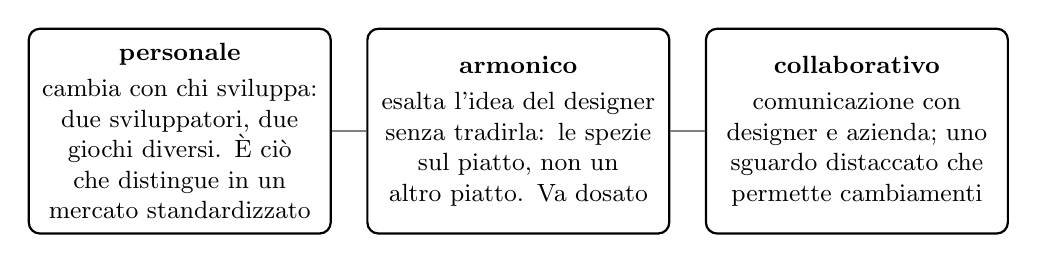
\begin{tikzpicture}[
  font=\small,
  a13pr/.style={draw, thick, rounded corners=4pt, text width=3.6cm, align=center,
                minimum height=2.6cm, fill=white},
]
  \node[a13pr] (p1) at (0,0) {\textbf{personale}\\[2pt]cambia con chi sviluppa: due
    sviluppatori, due giochi diversi. È ciò che distingue in un mercato
    standardizzato};
  \node[a13pr] (p2) at (4.3,0) {\textbf{armonico}\\[2pt]esalta l'idea del designer senza
    tradirla: le spezie sul piatto, non un altro piatto. Va dosato};
  \node[a13pr] (p3) at (8.6,0) {\textbf{collaborativo}\\[2pt]comunicazione con designer
    e azienda; uno sguardo distaccato che permette cambiamenti};
  \draw[thick, gray] (p1) -- (p2) -- (p3);
\end{tikzpicture}
\caption{I tre principi dello sviluppo secondo Marta.}
\label{a13:fig:principi}
\end{figure}

% ---------------------------------------------------------------------
\section{Gli \emph{stakeholder}: chi ha voce sul gioco}
\label{a13:sec:stakeholder}

\slidefig{img/AGD/agd13-stakeholder}{Gli stakeholder.}{slide \emph{Sviluppo di giochi}}{fig:agd13-stakeholder}


Chi sono, più nel dettaglio, gli \emph{stakeholder} tra cui lo sviluppo media? I primi
due sono già emersi: \textbf{il designer} (o la designer) e \textbf{la casa editrice}. Ma
una parte che ``molto spesso viene trascurata e tralasciata'' è \textbf{chi poi gioca il
gioco}: i clienti, le clienti. Quando si fa un gioco è importante ricordarsi \textbf{per
chi lo si sta facendo}, e quella è proprio la voce che non si sente: in una riunione
sul gioco c'è la casa editrice, nella veste del direttore editoriale, c'è l'autore o
l'autrice, ma \textbf{non c'è chi poi lo compra e lo gioca}, ``perché non si può''. Al
massimo si prendono dei \emph{playtester}, ma è una visione parziale; oppure, con un po'
di esperienza del mercato e delle persone a cui il gioco arriva, si può \textbf{fare le
veci di quella parte}. Marta lo fa spesso: ``sì, ma questa modifica va nell'interesse di
chi compra il gioco? Magari è una cosa che piace a noi qua dentro, ma a chi lo compra non
interessa''.

Non è detto che le tre parti ci siano sempre: quando c'è una casa editrice è probabile
che ci sia anche un cliente, ma possono mancare altre parti, o essercene altre ancora.
Se il gioco è \textbf{su licenza}, uno \emph{stakeholder} è \textbf{chi ha fornito la
licenza}, che ha i suoi vincoli e i suoi paletti. Può esserci una persona che ha
\textbf{scritto il \emph{world building}} del gioco e vuole che venga mantenuto in un
certo modo. ``Anche qua potrebbero esserci molte più variabili di quelle che viene da
pensare in prima battuta.''

\begin{figure}[htbp]
\centering
\begin{tikzpicture}[
  font=\small,
  a13st/.style={draw, thick, rounded corners=4pt, text width=2.7cm, align=center,
                minimum height=1.1cm, fill=white},
  a13opt/.style={draw, thick, dashed, rounded corners=4pt, text width=2.7cm, align=center,
                 minimum height=1.1cm, fill=white},
  a13arr/.style={{Stealth[length=2.5mm]}-{Stealth[length=2.5mm]}, thick}
]
  \node[draw, very thick, circle, fill=gray!15, minimum size=2.4cm, align=center] (sv)
    at (0,0) {\textbf{sviluppo}\\(mediazione)};
  \node[a13st] (des) at (-4.2,1.6) {\textbf{designer}\\la visione originale};
  \node[a13st] (pub) at (4.2,1.6) {\textbf{casa editrice}\\catalogo, mercato,
    reparti};
  \node[a13st, fill=gray!8] (cli) at (0,-2.9) {\textbf{chi gioca}\\(la voce che non c'è
    alle riunioni)};
  \node[a13opt] (lic) at (-4.2,-1.6) {chi ha dato la \textbf{licenza}};
  \node[a13opt] (wb) at (4.2,-1.6) {chi ha scritto il \textbf{\emph{world building}}};
  \foreach \n in {des,pub,cli}{\draw[a13arr] (sv) -- (\n);}
  \foreach \n in {lic,wb}{\draw[a13arr, dashed] (sv) -- (\n);}
\end{tikzpicture}
\caption{Gli \emph{stakeholder} di un gioco secondo la lezione. In tratteggio quelli che
ci sono solo in alcuni progetti. La voce di chi gioca arriva solo attraverso i
\emph{playtest} o attraverso chi sviluppa, che con l'esperienza ne fa le veci.}
\label{a13:fig:stakeholder}
\end{figure}

\paragraph{Approfondimento: partecipanti e ``avvocati''.} Bateman e Boon, in \emph{21st
Century Game Design}, aprono il libro con un principio che chiamano \emph{Zen Game
Design}: ``il game design deve essere privo di ego, bilanciando i desideri e i bisogni di
tutti i partecipanti''. I \emph{partecipanti} sono chiunque abbia un interesse nel
progetto (il pubblico, l'editore, lo studio, i programmatori, gli artisti, il marketing,
e, ``sempre più spesso'', il \emph{detentore della licenza}); poiché non tutti possono
partecipare al \emph{design}, alcune figure fanno da \emph{advocate}, da portavoce, per
gli altri. Gli autori notano proprio ciò che nota Marta: per il pubblico, di solito,
\emph{non c'è} un portavoce formale, e il compito ricade su chi progetta; e a proposito
della licenza consigliano di tenere aperto il dialogo durante tutto lo sviluppo, invece di
mostrare il gioco finito al licenziatario ed essere costretti a cambiarlo quando i
cambiamenti costano di più. Il libro parla di videogiochi, e di \emph{designer} più che
di sviluppatori, ma la figura che Marta descrive (chi si fa carico delle voci assenti)
corrisponde quasi esattamente al loro \emph{advocate}.

% ---------------------------------------------------------------------
\section{\emph{Design} contro sviluppo}
\label{a13:sec:designvs}

\slidefig{img/AGD/agd13-design}{Design e sviluppo a confronto.}{slide \emph{Sviluppo di giochi}}{fig:agd13-design}


Qui arriva, dice Marta, ``la differenza più sostanziale'' tra \emph{design} e sviluppo.
Avverte subito che è una visione ``un po' stereotipica'': non è detto che chi fa
\emph{design} abbia tutte queste caratteristiche, né chi fa sviluppo tutte le altre; ma
è ``una buona cartina di tornasole'' per distinguere le due figure. Il confronto è
riassunto nella tabella~\ref{a13:tab:designvs}.

\paragraph{Chi fa \emph{design}.}
\begin{itemize}
  \item \textbf{Non è \emph{time driven}}: normalmente non ha una scadenza vera e propria.
        Può pensare a una scadenza nel senso di ``questo \emph{design} tra cinque anni non
        è più interessante'', ma di base non ha ristrettezze temporali. Diverso è il caso di
        un \emph{design} su commissione.
  \item Ha \textbf{piena libertà creativa}: può muoversi liberamente, presentare qualsiasi
        idea e cercare il canale giusto per pubblicarla, senza vincoli.
  \item Ha di solito un \textbf{attaccamento emotivo}: il gioco l'ha creato, c'è qualcosa
        di suo. È positivo, perché permette di mettere nel gioco caratteristiche che una
        persona senza quell'amore per il progetto non metterebbe; ed è negativo, perché
        rende difficile fare modifiche, e a volte stravolgimenti, ``perché magari ci si è
        affezionati''.
  \item Ha l'\textbf{originalità}: si può prendere qualsiasi cosa e metterla dentro.
        ``Vado a prendere dei cubetti d'oro, di oro vero, e li metto nel gioco'':
        chi fa \emph{design} potrebbe volerlo fare, e il \emph{design} non lo impedisce; il
        problema, semmai, sarà della casa editrice. Ed è proprio lì che vengono fuori le
        cose ``un po' rivoluzionarie'' che a volte servono per smuovere i mercati, per
        alzare l'asticella.
  \item Ha \textbf{un'idea}: l'idea di partenza è ciò che caratterizza il \emph{design}.
        Non deve essere ``fatta e finita'', né completamente bilanciata, né
        completamente finalizzata: deve far capire le intenzioni. Negli anni c'è stata una
        \textbf{professionalizzazione del \emph{design}}, e oggi i designer portano in
        genere il progetto molto più avanti che in passato; ma resta la possibilità di
        dichiarare chiusa un'idea in qualsiasi momento (``questo è sufficiente per far
        capire che cosa dovrebbe essere sviluppato'') e consegnarla a una casa editrice.
\end{itemize}

\paragraph{Chi fa sviluppo.}
\begin{itemize}
  \item Ha \textbf{scadenze}: il \textbf{\emph{time to market}}, cioè quando il gioco deve
        uscire per prendere la spinta giusta del mercato, e il \textbf{vincolo del
        contratto} firmato tra casa editrice (o chi sviluppa) e designer. A un certo punto
        il gioco deve uscire, essere finalizzato, completato.
  \item Ha \textbf{restrizioni produttive}: tornando ai cubetti d'oro, ``io poi devo fare i
        conti con la realtà di mettere dei cubetti d'oro su mille scatole''. Come si fa?
        Sono veramente necessari? Sono veramente la cosa che serve?
  \item Esercita il \textbf{distacco}: non avendo un legame emotivo con il progetto,
        soprattutto all'inizio, può analizzarlo in modo più freddo e riconoscere quali
        caratteristiche servono all'idea per funzionare sul mercato, per certi clienti.
  \item Porta la \textbf{standardizzazione}, che ha due facce. È positiva perché un'idea
        troppo originale può spaventare alcune fette di mercato: un gioco molto originale
        viene recepito ``in modo misto, se va bene'', spesso male, perché il mercato ``non
        è pronto'', non aveva in mente quel gioco. La standardizzazione \textbf{smussa gli
        angoli}, rende il gioco più digeribile, più simile ad altre cose. Ma smussare gli
        angoli rischia anche di \textbf{portare via le caratteristiche importanti} del
        gioco.
  \item Ha l'\textbf{esperienza}\footnote{In questo punto la trascrizione è coperta da
        alcune righe di frasi ripetute senza senso (``è falsata da un pubblico''); la
        quinta voce della slide si ricostruisce dal discorso che segue e dalla sezione
        successiva, dedicata proprio all'esperienza.}: un designer che ha fatto un solo
        gioco ha ``pochissima'' esperienza, mentre chi fa sviluppo ha in genere lavorato a
        più titoli, perché si muove più rapidamente tra più progetti. Sa già dire ``questa
        cosa su itch.io non funziona, perché se lo pubblichi così le persone non capiscono
        neanche che tipo di gioco è: perché non evidenziamo questi aspetti?''. Un prodotto
        sullo scaffale, o caricato su itch.io, funziona?
\end{itemize}

\begin{table}[htbp]
\centering
\small
\begin{tabular}{@{}p{3.0cm}p{5.0cm}p{5.4cm}@{}}
\toprule
 & \textbf{Chi fa \emph{design}} & \textbf{Chi fa sviluppo} \\
\midrule
Tempo & non \emph{time driven} (salvo commissione) & scadenze: \emph{time to market},
  contratto \\
Libertà & piena libertà creativa & restrizioni produttive (i ``cubetti d'oro'' su mille
  scatole) \\
Rapporto col gioco & attaccamento emotivo (pro e contro) & distacco, analisi ``fredda'' \\
Direzione & originalità, anche rivoluzionaria & standardizzazione: smussa gli angoli
  (pro e contro) \\
Che cosa porta & un'idea, anche non finita & esperienza su molti titoli e generi \\
\bottomrule
\end{tabular}
\caption{\emph{Design} contro sviluppo secondo la slide di Marta: una visione volutamente
``stereotipica'', utile come cartina di tornasole. Nella realtà i confini sono sfumati.}
\label{a13:tab:designvs}
\end{table}

\paragraph{Confini sfumati.} Che cosa succede se un'idea è \textbf{troppo embrionale}? O se
un'implementazione che si va a fare \textbf{cambia l'esperienza di gioco}? ``Queste sono
domande importantissime, dove le cose si sfumano.'' A volte si ricevono idee così
embrionali che quasi non converrebbe prenderle, perché c'è così tanto sviluppo da fare
che non si sa più quanto è sviluppo e quanto è \emph{design}. Dall'altra parte c'è il
rischio che fare sviluppo \textbf{comprometta l'esperienza originale}. Questi ruoli vanno
immaginati come ``qualcosa di molto permeabile'', e non è mai facile mettere l'asticella
nel punto giusto: ``io molto spesso me lo chiedo: ma per questo gioco ho fatto
effettivamente sviluppo? Sono arrivata addirittura a fare \emph{design}?''. Con
l'esperienza diventa più facile tracciare la linea: capire se l'idea è davvero troppo
embrionale, e quindi non conviene svilupparla, o se c'è stato un eccesso (``ho fatto
troppo sviluppo, ho cambiato l'idea di partenza'') e bisogna tornare sui propri passi e
far emergere di più l'idea originale del designer.

% ---------------------------------------------------------------------
\section{Lo sviluppo è esperienziale}
\label{a13:sec:esperienza}

Marta lo ha detto più volte: lo sviluppo \textbf{si fonda sull'esperienza}. Da qualche
parte si parte, ``ci si improvvisa un po', come in tutte le cose'', ma poi l'esperienza si
accumula e fa la differenza. Non c'è un modo esatto di accumularla, ma c'è una differenza
di fondo tra le due figure.

\paragraph{Il designer focalizzato.} Chi fa \emph{design} può fare continuamente lo stesso
\emph{design}, senza esplorare tanti giochi e tante idee diverse. L'esempio è \textbf{Uwe
Rosenberg}\footnote{Nella trascrizione solo ``Rosenberg''; dal contesto (piazzamento
lavoratori, piazzamento tessere) è quasi certamente Uwe Rosenberg, l'autore di
\emph{Agricola}, citato più avanti nella lezione.}, che ha ``tre o quattro temi'' e tende
a fare giochi su quelli: il piazzamento lavoratori, il piazzamento tessere, e poi qualche
esperimento su altri generi. Una visione non ristretta in senso negativo, precisa Marta:
``\textbf{focalizzata} è il termine giusto''. Una visione che, nella sua iteratività, lo ha
portato a raggiungere \textbf{l'apice dei generi} in cui ha lavorato, perché li ha
``talmente tanto sviscerati'' da conoscerne forze e debolezze.

\paragraph{Lo sviluppatore che tocca tutto.} Chi sviluppa, al contrario, entra in contatto
con \textbf{tantissimi generi diversi}, perché le idee non vengono sempre dalla stessa
persona. Marta ha sviluppato giochi che durano più di due ore, giochi leggeri,
\emph{party game}, giochi di destrezza astratti: ``si tocca un po' tutto quello che
esiste''. Vale anche per il gioco di ruolo, dove chi sviluppa può muoversi più facilmente
tra sistemi diversi, dal gioco di una pagina (\emph{one page}) al manuale di 50 pagine con
campagna.

% ---------------------------------------------------------------------
\section{Il rapporto tra chi progetta e chi sviluppa}
\label{a13:sec:rapporto}

\slidefig{img/AGD/agd13-rapporto}{Il rapporto tra designer e developer.}{slide \emph{Sviluppo di giochi}}{fig:agd13-rapporto}


L'esperienza passa anche attraverso il \textbf{rapporto tra designer e \emph{developer}},
che ``deve essere saputo gestire'': per le differenze appena viste, per i livelli diversi
di esperienza, per i ruoli diversi, che a volte sembrano perfino contrapposti. Ma è, come
detto all'inizio, un rapporto di mediazione, e la cosa importante è \textbf{trovare i
compromessi}. Ogni rapporto è diverso: non si lavora con tutti i designer nello stesso
modo.

\paragraph{Collaborazione attiva e passiva.} A Marta sono capitate entrambe.
\begin{itemize}
  \item Una \textbf{collaborazione attiva} è uno \textbf{scambio ricorrente} tra le due
        parti: ci si aggiorna a vicenda, si fanno cambiamenti, ``ci si rimbalzano molto le
        idee e il progetto''.
  \item Una \textbf{collaborazione passiva} è quando una delle due parti prende in carico
        la maggior parte del lavoro e \textbf{riceve dei \emph{feedback}} dall'altra, e il
        rapporto si limita a questo. Può capitare, per esempio, che un gioco venga
        valutato, firmato con la casa editrice, e che poi chi l'ha progettato
        ``praticamente sparisca''. \textbf{È legittimo}: l'idea è stata fornita, i dubbi, se
        c'erano, si spera siano stati risolti, e magari il designer non ha interesse a
        vedere come si sviluppa il gioco da lì in poi, e vuole vederlo solo a cose fatte.
\end{itemize}

\paragraph{Le aspettative.} È importante anche \textbf{gestire le aspettative}: ricordarsi
che quando un gioco passa per altre persone \textbf{viene inevitabilmente modificato}.
``Un gioco è un processo di collaborazione'': non c'è una sola persona che lo fa. La
figura del designer è stata più volte messa in primo piano, ma il processo è
\textbf{collettivo}: il gioco non arriverebbe sullo scaffale senza chi lo produce, chi fa
la grafica e le illustrazioni, e chi lo sviluppa. Affidando un gioco a una casa editrice
o a chi sviluppa, il gioco \textbf{cambierà}, anche in modi che non sempre troveranno
d'accordo. L'importante è trovare i compromessi giusti.

\paragraph{La fiducia.} E qui viene l'ultimo punto: la \textbf{fiducia}. ``Come se si
vogliono avere delle relazioni nella vita'', bisogna avere una fiducia reciproca. Il
consiglio di Marta, anche ai designer: \textbf{cercatevi case editrici, sviluppatori o
sviluppatrici con cui pensate che possa esserci un buon rapporto di fiducia}, perché i
rapporti vanno male soprattutto quando questa fiducia viene a mancare, quando una delle
due parti pensa che l'altra ``non stia facendo gli interessi del gioco''.

% ---------------------------------------------------------------------
\section{Da dove viene il ruolo: \emph{developer} ed \emph{editor}}
\label{a13:sec:storia}

\slidefig{img/AGD/agd13-storia}{Brevi cenni storici sullo sviluppo.}{slide \emph{Sviluppo di giochi}}{fig:agd13-storia}


``Vi siete chiesti chi è l'\emph{editor}, in questo calderone?'' Per rispondere Marta
racconta da dove nasce la figura dello sviluppo.

\paragraph{Gli anni Settanta e i \emph{wargame}.} Siamo negli anni '70, e la
\textbf{SPI}, \emph{Simulations Publications, Inc.}\footnote{Marta dice ``Simulation
Publishing Inc., credo''; il nome corretto della casa editrice americana di
\emph{wargame} è \emph{Simulations Publications, Inc.}}, una casa editrice americana di
\emph{wargame}, ha bisogno di pubblicare \textbf{più \emph{wargame}}: chi fa \emph{design}
``non ce la fa a fare tutti questi''. A questo punto la trascrizione si interrompe per
alcune frasi ripetute senza senso, e una parte del racconto va perduta\footnote{Coprono
la spiegazione di come la SPI risolse il problema. Il capitolo non la ricostruisce; si
sa, in generale, che nella SPI il \emph{developer} era la figura che riceveva il
\emph{design} e lo portava a un gioco pubblicabile, ma la trascrizione non permette di
dire che cosa abbia detto Marta.}. Quando il discorso riprende, Marta sta elencando le
case editrici che, dopo, hanno deciso di \textbf{inserire degli sviluppatori}:
\textbf{Fantasy Flight}, la linea \textbf{\emph{alea}} di Ravensburger e \textbf{Hans im
Glück}\footnote{Nella trascrizione ``la linea Alia di Ravensburger'' e ``Huntington
Gluck'', poi ``Hansingluck''.}. Gli sviluppatori sono ``fondamentalmente delle figure che
fanno le veci dei designer all'interno delle aziende'', ma \textbf{non sono designer in
senso stretto}: avranno idee e visioni diverse, ed è qui che nasce il rapporto
collaborativo come lo conosciamo oggi.

\paragraph{L'\emph{editor} tedesco.} Contemporaneamente c'era un'altra figura,
l'\textbf{\emph{editor}}, molto diffusa in \textbf{Germania}: era la persona che si
occupava di \textbf{portare il gioco a compimento}. Le altre case editrici tedesche avevano
un \emph{editor}, e lo avevano anche \emph{alea} e Hans im Glück; ma l'\emph{editor}
\textbf{non si occupava del gioco nell'aspetto meccanico e regolistico}: si occupava di
tutti gli altri aspetti.

\paragraph{L'inversione.} Andando avanti le due figure \textbf{si sono ibridate}, e oggi si
sono ``un po' invertite'': lo \textbf{sviluppo}, che prima si occupava solo della parte
meccanica, oggi prende in carico \textbf{tutti gli aspetti}, compresa la parte meccanica;
l'\textbf{\emph{editor}} ha un ruolo più piccolo, legato soprattutto \textbf{alle parole}:
rivede i testi, controlla che siano in italiano corretto, si accerta che tutto sia
presentato al meglio. Questa è, oggi, la figura che di solito si chiama \emph{editor} nel
gioco da tavolo. Ma non è definito in modo assoluto: ci sono case editrici che chiamano
``sviluppatore'' chi fa \emph{editing}, e case che fanno \emph{editing} e non hanno
sviluppatori. È una figura nata negli ultimi anni e \textbf{non c'è ancora una
standardizzazione}; questa, confrontandosi con colleghi e colleghe di altre aziende, è la
tendenza che Marta vede.

\begin{figure}[htbp]
\centering
\begin{tikzpicture}[
  font=\small,
  a13ev/.style={draw, thick, rounded corners=3pt, text width=3.5cm, align=center,
                minimum height=1.4cm, fill=white},
  a13arr/.style={-{Stealth[length=3mm]}, thick}
]
  \draw[a13arr] (0,0) -- (13.4,0);
  \foreach \x/\lab in {1.6/anni '70, 6.4/poi, 11.4/oggi}{
    \fill (\x,0) circle (2.5pt);
    \node[below=4pt, font=\footnotesize] at (\x,0) {\lab};
  }
  % sopra: developer
  \node[a13ev, above=0.5cm] at (1.6,0) {SPI (\emph{wargame}): servono più giochi di quanti
    i designer riescano a farne};
  \node[a13ev, above=0.5cm] at (6.4,0) {Fantasy Flight, \emph{alea} (Ravensburger), Hans
    im Glück inseriscono gli \textbf{sviluppatori}: parte meccanica};
  \node[a13ev, above=0.5cm, fill=gray!12] at (11.4,0) {\textbf{sviluppo}: tutti gli
    aspetti, meccanica compresa};
  % sotto: editor
  \node[a13ev, below=0.7cm] at (6.4,0) {l'\textbf{\emph{editor}} (soprattutto in Germania)
    porta il gioco a compimento, \emph{tranne} meccanica e regole};
  \node[a13ev, below=0.7cm, fill=gray!12] at (11.4,0) {\textbf{\emph{editor}}: le parole,
    i testi, la presentazione};
  \node[font=\footnotesize\itshape, rotate=90] at (-0.4,1.4) {\emph{developer}};
  \node[font=\footnotesize\itshape, rotate=90] at (-0.4,-1.5) {\emph{editor}};
\end{tikzpicture}
\caption{Come Marta racconta la nascita delle due figure e la loro ``inversione''. Le
date intermedie non sono dette, e una parte del racconto è persa nella trascrizione. Oggi
le definizioni non sono ancora standardizzate.}
\label{a13:fig:storia}
\end{figure}

\paragraph{Prima pausa.} ``Siamo alla seconda parte'': Marta propone una pausa di una
decina di minuti e invita a portare domande al ritorno. Durante la pausa la trascrizione
registra il commento su un videogioco di cui si è detto nelle avvertenze, e poi diversi
minuti di frasi ripetute in ciclo. Quando si riprende, uno studente avverte che sta
ancora mangiando, ``ma ci sono, nessun problema''. Marta chiede se ci sono domande o
curiosità (``non so se vi posso rispondere in pieno, perché c'è una parte di segreto
professionale, ma possiamo ingegnarci'').

% ---------------------------------------------------------------------
\section{Il conflitto di interessi}
\label{a13:sec:conflitto}

La prima domanda è di \textbf{Gianmarco}\footnote{Più avanti Marta si riferisce a questa
domanda come ``quella domanda che ha fatto Gianmarco''.}, ``fra la curiosità e la
provocazione'': lo sviluppatore, di solito, è \textbf{assunto dalla casa editrice}, mentre
il designer non lo è necessariamente. \textbf{Non c'è un conflitto di interessi} nel fare
da mediatore tra due parti, quando si è assunti da una delle due? ``È un'ottima domanda,
onestamente'', risponde Marta, ``non so neanche se riuscirò a soddisfarti''.

\paragraph{Com'era prima.} All'inizio la figura non c'era, e il rapporto era diverso: i
designer avevano un gioco e la casa editrice si limitava a \textbf{metterlo sul mercato
così com'era stato pensato}; rivedeva i testi, curava la produzione fisica. ``Addirittura
i designer brevettavano i tabelloni'': erano tempi diversi. Funzionava quando \textbf{il
mercato era piccolo}, le idee erano poche e c'era tantissimo spazio per presentarle.

\paragraph{Com'è oggi.} Oggi a \textbf{Essen}, la più grande fiera al mondo di giochi da
tavolo, secondo le ultime stime che Marta ricorda si parla di qualcosa come \textbf{2500
nuovi giochi presentati in un solo anno}, e solo tra quelli pubblicati in qualche forma,
senza contare tutta la realtà indipendente che pubblica su itch.io e simili. ``Il volume
di giochi presentati ogni anno è spaventoso.'' Le case editrici, molto spesso,
\textbf{non possono permettersi di sbagliare un titolo} (``cannare'', dice Marta): dipende
dalle dimensioni, ma una piccola casa editrice che sbaglia anche solo un paio di titoli
può chiudere, perché \textbf{l'investimento nel gioco analogico è importante}. Per questo la
cosa fondamentale è che il gioco \textbf{rispetti le aspettative di mercato}. E chi fa
\emph{design} non è tenuto a conoscerle, e probabilmente non ha i mezzi per farlo: Marta
non conosce ``tantissime designer'' che abbiano la possibilità di andare a Essen e
interfacciarsi con più editori, anche internazionali. È un limite, e oggi \textbf{avere
dentro l'azienda una figura che fa le tue veci} per tutte queste questioni è generalmente
visto come positivo, anche se non vale per tutte le persone.

\paragraph{Che cosa fa Marta.} Marta sconsiglia spesso di fare giochi \textbf{solo con
l'obiettivo di pubblicare con una casa editrice}: capisce che i soldi facciano gola, ma
bisogna saper riconoscere \textbf{quali giochi sono adatti al mercato}, trovare la casa
editrice che fa per noi e vedere se con le persone con cui si collabora ci si trova bene.
Lei, da parte sua, cerca di \textbf{rispettare le volontà del designer}, proprio perché sa
di essere assunta dalla casa editrice, ma anche di essere, in quel momento,
\textbf{l'unica persona che sta parlando per il designer}, che magari non c'è a tutte le
riunioni: diventa importante difendere le sue idee. Si rende conto che non è sempre
facile, e che non è facile nemmeno accettare la dinamica. ``In un mondo ideale'' chi fa
\emph{design} potrebbe partecipare attivamente alle quaranta ore lavorative in azienda in
cui si fanno le cose; nella realtà le dinamiche sono complesse. Gianmarco si dice
soddisfatto: ``mi è abbastanza chiara la risposta''.

\paragraph{Approfondimento: il portavoce assunto.} La domanda di Gianmarco è la stessa che
Bateman e Boon si pongono a proposito del produttore esterno, il portavoce dell'editore
nei progetti di videogiochi: secondo loro molti sviluppatori ne risentono
l'``interferenza'', ma il problema nasce di solito quando il portavoce cerca di
\emph{prendersi il controllo} del \emph{design}, invece di rappresentare i bisogni di chi
rappresenta. La risposta di Marta sposta il problema nello stesso punto: il ruolo regge
finché chi sviluppa si comporta da mediatore, e dà voce anche a chi, in quella stanza, non
c'è.

% ---------------------------------------------------------------------
\section{Le otto fasi dello sviluppo}
\label{a13:sec:fasi}

\slidefig{img/AGD/agd13-fasi}{Le otto fasi dello sviluppo.}{slide \emph{Sviluppo di giochi}}{fig:agd13-fasi}


Oggi, ripete Marta, si fa un'infarinatura generale; la prossima volta qualche esempio più
pratico e qualche tecnica. ``La realtà della faccenda è che \textbf{non c'è un modo esatto
di procedere}'': ogni gioco fa storia a sé, e non si sviluppa un gioco totalmente
narrativo come si sviluppa un gioco di destrezza. Raccomanda di \textbf{pensare in modo
elastico}, perché è facile farsi ingannare e pensare che le cose siano lineari: ``non è mai
così''. Ed è anche l'aspetto bello del lavoro: c'è sempre una sfida nuova. ``Io mi sono
improvvisamente scoperta appassionata di bonsai soltanto perché ho lavorato a un gioco che
parlava di bonsai'': se si è persone curiose, ``è un bel lavoro''.

Marta ha riassunto il lavoro in \textbf{otto fasi} (figura~\ref{a13:fig:fasi}):
\textbf{selezione}, \textbf{ricerca}, \textbf{concettualizzazione},
\textbf{presentazione}, \textbf{\emph{testing}}, \textbf{implementazione},
\textbf{preparazione degli \emph{asset}}, \textbf{revisioni}. È, grosso modo, la
\emph{pipeline} di un gioco dal primo momento in cui viene accettato nel ramo di sviluppo
di un'azienda a quando lascia l'azienda per essere stampato e finire sullo scaffale. Le
fasi \textbf{non si svolgono necessariamente in quest'ordine}: a volte si torna indietro, a
volte mancano dei pezzi; c'è tanto scambio e tanto dialogo con tutti i reparti per
arrivare alla fine ``nel modo più celere possibile'', ma ``molto spesso arrivano i
disastri e bisogna tornare indietro''. In questa lezione Marta arriva fino alla
preparazione degli \emph{asset}; le \textbf{revisioni} e il \textbf{come scrivere un
regolamento} restano per venerdì (sezione~\ref{a13:sec:chiusura}).

\begin{figure}[htbp]
\centering
\begin{tikzpicture}[
  font=\small,
  a13ph/.style={draw, thick, rounded corners=3pt, text width=2.3cm, align=center,
                minimum height=1.0cm, fill=white},
  a13arr/.style={-{Stealth[length=2.5mm]}, thick}
]
  \node[a13ph] (f1) at (0,1.6) {1.\ selezione};
  \node[a13ph] (f2) at (3.1,1.6) {2.\ ricerca};
  \node[a13ph] (f3) at (6.2,1.6) {3.\ concettua-\\lizzazione};
  \node[a13ph] (f4) at (9.3,1.6) {4.\ presentazione};
  \node[a13ph] (f5) at (9.3,-0.6) {5.\ \emph{testing}};
  \node[a13ph] (f6) at (6.2,-0.6) {6.\ implementa-\\zione};
  \node[a13ph] (f7) at (3.1,-0.6) {7.\ preparazione\\degli \emph{asset}};
  \node[a13ph, fill=gray!12] (f8) at (0,-0.6) {8.\ revisioni\\(venerdì)};
  \draw[a13arr] (f1) -- (f2);
  \draw[a13arr] (f2) -- (f3);
  \draw[a13arr] (f3) -- (f4);
  \draw[a13arr] (f4) -- (f5);
  \draw[a13arr] (f5) -- (f6);
  \draw[a13arr] (f6) -- (f7);
  \draw[a13arr] (f7) -- (f8);
  \draw[a13arr, dashed] (f2.north) to[bend right=35] node[above, font=\footnotesize]
    {si torna indietro} (f1.north);
  \draw[a13arr, dashed] (f6.south) to[bend right=40] node[below, font=\footnotesize]
    {ogni ciclo di \emph{test}} (f5.south);
  \draw[a13arr, dashed] (f5.south west) to[bend left=25] (f6.south east);
  \node[font=\footnotesize, text width=4.2cm, align=left, anchor=west] at (-1.2,-2.9)
    {\emph{ingresso}: un prototipo accettato};
  \node[font=\footnotesize, text width=4.2cm, align=right, anchor=east] at (10.5,-2.9)
    {\emph{uscita}: il gioco va in stampa};
\end{tikzpicture}
\caption{Le otto fasi dello sviluppo secondo Marta. L'ordine è indicativo: le frecce
tratteggiate ricordano che si torna spesso indietro (per esempio la ricerca informa la
selezione, e implementazione e \emph{testing} si alternano in ciclo).}
\label{a13:fig:fasi}
\end{figure}

% ---------------------------------------------------------------------
\section{La selezione}
\label{a13:sec:selezione}

\slidefig{img/AGD/agd13-selezione}{La selezione.}{slide \emph{Sviluppo di giochi}}{fig:agd13-selezione}


La selezione comincia quando si riceve un \textbf{prototipo}, e se ne ricevono
\textbf{tantissimi}. Marta non sa fare una stima precisa, perché cambia molto da periodo a
periodo e da casa editrice a casa editrice; ma nell'ultimo mese, se non sbaglia, a dV
Giochi ne sono arrivati \textbf{una sessantina}. dV è una casa editrice grande, e altre ne
ricevono meno; ma si immagini di dover valutare 60 prototipi al mese: ci deve essere
\textbf{una cernita}, e avviene in vari modi.

\begin{itemize}
  \item \textbf{Catalogo e mercato di riferimento.} C'è una scrematura iniziale legata al
        catalogo. dV Giochi non pubblica giochi che superano i \textbf{45 minuti, un'ora}:
        se arriva un gioco che dura due ore e mezza, probabilmente viene scartato a
        priori, perché è molto improbabile che faccia al caso loro. Un'occhiata si dà
        sempre, però: magari c'è un'idea buona, magari le due ore e mezza sono una stima
        sbagliata dell'autore.
  \item \textbf{La complessità.} Un buon gioco può risultare \textbf{eccessivamente
        complesso}, nel senso che è difficile da spiegare e da far capire, e allora non ci
        sono i margini per provarlo e testarlo adeguatamente: ``magari devo studiarmi un
        regolamento per quattro giorni, e io quattro giorni da passare a provare un gioco
        non ce li ho''. Va valutato: è un gioco che si può testare con il designer? Fa
        davvero al caso nostro?
  \item \textbf{La sensibilità del \emph{team} editoriale.} Lo sviluppo è personale, e
        questo si riflette in tutto: ``se non ci piacciono i giochi in tempo reale, è
        inutile che pensiamo che quel gioco in tempo reale funzioni benissimo'', perché se
        poi non riusciamo a metterci a svilupparlo stiamo solo perdendo tempo. In ambito
        professionale non contano solo le preferenze (``altrimenti io svilupperei solamente
        due tipi di giochi''), ma ci sono giochi che si sa che non funzioneranno con quel
        \emph{team}. Marta, per esempio, ``non è ferratissima'' sui \textbf{giochi di
        destrezza}: tende a evitarli o a passarli a un collega (``tu che hai più la
        sensibilità per questa cosa, ci vedi qualcosa in questo gioco?''), perché anche
        fisicamente fa fatica a valutarli. Una casa editrice brava riesce a riflettere
        queste sensibilità nel suo catalogo. E bisogna tenerle a mente perché i giochi
        selezionati vanno poi testati, provati, discussi con i designer: ``quello che inizia
        come un processo di un'ora, un'ora e mezzo potrebbe diventare tranquillamente di
        giorni''.
  \item \textbf{La coerenza sull'asse tema--meccaniche.} Negli ultimi anni ci sono
        tantissimi giochi che si assomigliano. Una volta si tendeva a privilegiare uno dei
        due aspetti, di solito le meccaniche, e poi c'era il cosiddetto \textbf{\emph{window
        dressing}}: si ``appiccicava'' sopra un tema che giustificasse un po' le
        meccaniche. Negli anni questo ha portato a una \textbf{stagnazione}, e oggi c'è
        anche ``un po' di pesantezza'' da questo punto di vista. Oggi è molto importante che
        \textbf{meccaniche e tema si parlino in modo molto stretto}. Questo significa che il
        gioco si può modificare di meno, e che c'è più rischio che non venga accettato:
        ``lato designer è un incubo'', perché si lavora a un gioco per tantissimo tempo e
        poi non viene accettato perché non piace il tema, e se il legame è forte non si
        può più dire ``cambia il tema, qual è il problema?''. Ma è anche ciò che oggi fa
        scegliere un gioco sopra gli altri. L'esempio è \textbf{\emph{Hegemony}}\footnote{Nella
        trascrizione ``Egemoni''; si tratta con ogni probabilità di \emph{Hegemony: Lead
        Your Class to Victory}, un gioco gestionale sulle classi sociali e sulla politica
        economica di uno Stato.}, un gioco gestionale (``vedo un sì'', dice Marta quando
        chiede se la classe lo conosce) che ricrea le dinamiche della politica di uno Stato
        ``in modo molto viscerale'': è una simulazione astratta, ma i designer hanno legato
        le meccaniche al tema ``in modo indissolubile''. Non si può prendere \emph{Hegemony}
        e farne un gioco sugli esploratori di \emph{dungeon}, ``perché non regge''; mentre su
        un gioco di carte con solo numeri si può mettere il \emph{dungeon}, o un tema
        diverso, perfino politico.
\end{itemize}
Sono criteri generici, ``che ci aiutano a selezionare i giochi più promettenti'', a capire
quali meritano una possibilità di sviluppo.

% ---------------------------------------------------------------------
\section{La ricerca}
\label{a13:sec:ricerca}

\slidefig{img/AGD/agd13-ricerca}{La ricerca.}{slide \emph{Sviluppo di giochi}}{fig:agd13-ricerca}


Dopo la selezione c'è la \textbf{ricerca}. Lo strumento principale, nel mondo del gioco da
tavolo, è \textbf{BoardGameGeek} (BGG): è ``il sito di riferimento'' perché è un
\textbf{\emph{database}}, ed è lo strumento più usato nell'industria, ``con tutti i limiti
che ha'': è una visione \textbf{americano-centrica}, perché la sua utenza è prevalentemente
quella. Ma resta indispensabile, perché vi si trovano tantissime informazioni.

\paragraph{Le domande della ricerca.} Si immagini di aver appena visto, e accettato, il
prototipo di \emph{Hegemony}: un gioco sulla politica e sugli Stati. Prima di tutto
bisogna capire:
\begin{itemize}
  \item ce ne sono altri sul mercato che fanno già la stessa cosa?
  \item se sì, che cosa fanno di diverso?
  \item quali caratteristiche li esaltano, o li affossano?
  \item come sono percepiti dalle persone?
  \item che cosa si può fare di diverso? Magari l'idea è valida, ma approfondendo si scopre
        che ci sono tanti giochi sulla politica di uno Stato: che cosa fa di diverso
        questo?
\end{itemize}
Si conoscono così i temi comuni: andando su BGG e guardando la classifica
\textbf{\emph{hotness}} del periodo, o leggendo le recensioni, emerge per esempio come
negli ultimi anni l'\textbf{asimmetria}\footnote{Nella trascrizione ``la simmetria'', qui e
più avanti (``\emph{Root} con la simmetria''); dal contesto, e dall'esempio di
\emph{Root}, che è il gioco asimmetrico per eccellenza, si tratta quasi certamente di un
errore di trascrizione per ``asimmetria''.} sia diventata una caratteristica molto
importante dei giochi di una certa complessità. Ci si crea anche delle
\textbf{metriche}: ``oggi vanno di più i giochi di dadi''. E qui si torna alla selezione:
``se abbiamo un gioco di dadi, magari è il momento di valutarlo''. È un processo ``che si
informa a sua volta''.

\subsection{Si può prevedere il mercato?}
\label{a13:sec:prevedere}

Uno studente alza la mano con una domanda ``molto complicata'', nata dalla sua esperienza:
ha lavorato molti anni nell'\textbf{\emph{automotive}}. Quando si progetta un'automobile si
prende a riferimento l'esistente: devo fare un nuovo SUV, identifico il cliente, faccio il
posizionamento di prodotto, studio chi c'è in quello spazio e rispetto a quello definisco
le caratteristiche. Ma per fare un'automobile, da foglio bianco, ci vogliono \textbf{dai
quattro ai sei anni}: quattro anni prima dell'uscita si studiano dei concorrenti pensati
sei anni prima. Come si fa, nel gioco, a capire che cosa sarà di tendenza quando il gioco
uscirà, probabilmente due o tre anni dopo la selezione?

\paragraph{``La risposta non piacerà mai a nessuno''.} \textbf{Non c'è un modo di prevedere
il mercato}, ma si può \textbf{affinare la sensibilità}. Su cicli di quattro--sei anni c'è
poco da fare: in sei anni il gioco da tavolo ``subirà degli scossoni importanti''. Prendendo
il 2026 come riferimento: sei anni fa, nel 2020, c'erano giochi che avevano iniziato a
stabilire la propria dimensione, come \textbf{\emph{Root}}, \textbf{\emph{Wingspan}},
\textbf{\emph{Terraforming Mars}}\footnote{Nella trascrizione ``Terraform in Mars''.}; e
questi giochi hanno fatto leva moltissimo su un \textbf{mazzo formato da tutte carte
diverse}, che fa cambiare l'esperienza da una partita all'altra per l'alta variabilità, o,
nel caso di \emph{Root}, sull'asimmetria. Ma sei anni prima ancora ``non c'era neanche
l'antipasto di queste cose'': con il senno di poi si riconosce qualche lieve segno dell'onda
che stava emergendo, ma era ``davvero troppo tempo''. Per questo i \textbf{cicli di
sviluppo} cercano di essere \textbf{il più brevi possibile}, anche se realisticamente è
difficile stare sotto i \textbf{due anni}: Marta ha fatto un conto, e per sviluppare un
gioco servono in media \textbf{nove mesi}; tra produzione e tutto il resto, quando il
gioco finisce sul mercato sono passati due anni.

\paragraph{Curiosità, sempre.} Quello che si può fare è \textbf{curare molto la propria
ricerca}: informarsi, avere curiosità, cercare di capire i giochi quando escono e le loro
peculiarità. Per esempio: \textbf{perché \emph{Magical Athlete} è diventato
improvvisamente così forte}, così centrale nella comunicazione? Che cosa ha fatto bene?
Si possono dare centinaia di risposte diverse; ma facendo questo lavoro la sensibilità si
affina e si riesce a ``vedere un po' in avanti''. È in parte una visione personale, che
viene dalle proprie esperienze, e in parte emerge dal conoscere il settore. Per fare
sviluppo, ``ma a me viene da dire anche per fare \emph{design}'', bisogna avere questa
tendenza a immaginare come sarà il mercato, ``che non significa prenderci in pieno'', ma
avere la sensibilità per capire dove si sta andando.

\paragraph{Il caso \emph{Magical Athlete}.} Quest'anno Marta non è andata a Essen con i
colleghi; al loro ritorno le hanno detto: ``Marta, non ci crederai mai, ma a Essen abbiamo
visto un sacco di prototipi con i dadi''. ``E certo'', ha risposto lei: \emph{Magical
Athlete} ``è uscito l'altro ieri''. Tra i designer è diventato ``una bomba''. Perché? Marta
lo paragona, ``parafrasando'', alla \emph{Fontana} di \textbf{Duchamp}, l'orinatoio esposto
come opera d'arte: un gesto rivoluzionario. \emph{Magical Athlete} è stato un po' quella
cosa lì: ha detto ``e se facessimo il gioco dell'oca, ma ancora più folle?'', e ha
centrato l'obiettivo. La nuova edizione è curata da \textbf{Richard Garfield}, ``che non è
l'ultimo degli arrivati'': è il creatore di \emph{Magic: The Gathering}, e ha fatto molti
altri \emph{design} di spessore. Il gioco, nei circoli di appassionati, era già conosciuto;
ma ha avuto questo ``volano incredibile'' per una ragione precisa.
\begin{itemize}
  \item Analizzando il percorso dei giochi da tavolo, negli ultimi anni la maggior parte
        dei giochi \textbf{davano tantissimo controllo}. Da \textbf{\emph{Agricola}}, uscito
        nel \textbf{2007}, fino al 2026, i giochi hanno esplorato a fondo la meccanica
        dell'avere tutto sotto il proprio controllo, tanto che \emph{Agricola} ha in un
        certo senso inaugurato i giochi \textbf{``multi-solitari''}, come li chiamiamo oggi:
        giochi in cui l'interazione è per lo più passiva, indiretta, in cui ognuno ``si fa
        le sue cose'' e poi si vede chi ha fatto più punti.
  \item La tendenza si è esasperata al punto che serviva una \textbf{risposta forte nella
        direzione opposta}: \emph{Magical Athlete} mette \textbf{tutto il caos possibile},
        fa emergere tutto da una grande interazione tra le persone, ed è un gioco
        \textbf{fortemente esperienziale ed emozionale}. Dice: ``alla fine non ti serve
        davvero tutto questo controllo per stare al tavolo e avere una serata piacevole
        con le persone con cui ti trovi bene''. ``È stato fondamentalmente un messaggio.''
  \item Garfield non ha ``la visione del futuro'', ma ha l'esperienza: ci ha cominciato a
        lavorare, se Marta ricorda bene, nel \textbf{2022}; ha capito che quello era il
        \emph{trend} e che poteva intercettarlo, e ha avuto anche fortuna, perché l'ha
        intercettato probabilmente nel momento di massimo picco, quando le persone
        volevano davvero qualcosa di diverso.
\end{itemize}
Una visione del futuro, quindi, ``un po' ce la si può creare'': si arriva a intravedere le
tendenze, a capire su che cosa si spinge di più. E stare dentro una casa editrice è un
\textbf{punto di vista privilegiato}: Marta conosce ``un sacco di giochi'' che usciranno
prossimamente ma non sono ancora stati annunciati, un po' per i \emph{partner}, un po'
perché nel settore ci si parla.

\paragraph{``Vedi già il prossimo \emph{trend}?''} Lo stesso studente (``non voglio
monopolizzare il discorso, ma ne avrei mille'') chiede ancora: provando i prototipi di
oggi, Marta riesce a intravedere un \emph{trend} che, fra due anni, sarà la reazione a
quello attuale, per esempio a tutti questi giochi di dadi? Marta vuole ``essere molto
onesta'' e non ``vendere false promesse'': secondo lei non è davvero possibile prevederlo,
ma \textbf{si può migliorare}. Nella sua stima, \textbf{su tre giochi che sviluppa, uno lo
sbaglia}, nel senso che non capisce benissimo dove va il mercato; gli altri due reagiscono
bene, e in azienda c'è soddisfazione perché i \emph{partner} li accettano, ``sentono che è
il momento giusto''. Non è una decisione solo sua: è di un intero \emph{team}. C'è un
\textbf{\emph{editor in chief}} che stabilisce la \textbf{linea editoriale}, c'è una
\textbf{parte commerciale} che dice ``ci servono giochi di questo tipo''. Ma quando vede un
prototipo deve sempre \textbf{immaginarsi come sarà sullo scaffale}: tutto il lavoro serve
a ottenere un gioco di cui si ha già contezza di come sarà, anche se l'idea iniziale potrà
non essere precisissima; ``l'importante è stare più o meno lì''. Lo studente conclude che
``per fare \emph{Magical Athlete} non basta solo la bravura, ci vuole anche un po' di
fortuna''.

\paragraph{\emph{Magical Athlete} e la fortuna del momento.} ``Ottimo esempio di tante
cose'', risponde Marta: \emph{Magical Athlete} è uscito nel \textbf{2003} ed è stato
abbastanza ignorato, senza il successo che ha oggi. Alcuni designer lo segnalavano come un
gioco di spessore, che veniva dal \textbf{Giappone} quando quello non era ancora un mercato
conosciuto e non si conoscevano i designer giapponesi. La \textbf{Z-Man}, casa americana
``molto sperimentale'', perché \textbf{Zev}, il suo \emph{editor}\footnote{Zev
Shlasinger, fondatore di Z-Man Games.}, prendeva sempre \emph{design} strani, aveva portato
\emph{Magical Athlete} in America, ma in modo modesto, ``e poi era sparito''. La casa che
l'ha rifatto\footnote{Nella trascrizione ``MYK'': con ogni probabilità CMYK, l'editore
americano della nuova edizione.} ha capito che ora era il momento molto più opportuno per
un gioco del genere: ha \textbf{cambiato completamente l'estetica e la presentazione}, lo
ha addirittura \textbf{semplificato}, e ha funzionato alla grande. ``A volte serve anche un
po' la fortuna, e capire qual è il momento giusto.'' La ricerca, quindi, è importante, e
serve anche ai designer; ma chi sviluppa, lavorando su tanti giochi, deve conoscere tutto
quello che esce: più si è carenti su questo aspetto, più si rischia di mettere sul mercato
qualcosa che esiste già. ``È difficile, però si fa. Ci si arrangia in qualche modo.''

% ---------------------------------------------------------------------
\section{La concettualizzazione: il \emph{Game Concept Document}}
\label{a13:sec:gcd}

\slidefig{img/AGD/agd13-gcd}{Il Game Concept Document.}{slide \emph{Sviluppo di giochi}}{fig:agd13-gcd}


Una cosa che aiuta molto, in tutto questo, è la \textbf{concettualizzazione}: quando la
ricerca è fatta e il gioco è selezionato, è il momento di capire \textbf{come dovrà essere
questo gioco}. Marta presenta uno strumento che usa e che trova ``utilissimo''.

\paragraph{Dal GDD al GCD.} Quando ha cominciato non esisteva niente del genere, ma serviva
qualcosa che informasse il \emph{team} di dove si è, che cosa si sta facendo e dove sta
andando il gioco, perché dal solo prototipo non è facile capirlo. All'inizio ha usato i
\textbf{GDD}, i \emph{Game Design Document}, noti a chi ``mastica un po' lo sviluppo
videoludico'': documenti lunghissimi, anche di 80--90 pagine, che delineano il videogioco
per intero prima di svilupparlo. Le erano utili per ricordarsi le cose, ma li trovava
``davvero tanto pesanti''. Da lì, lavorando, è venuto fuori un altro concetto, che poi ha
scoperto non essere solo suo, perché anche nel mondo videoludico cominciava a essere
applicato: il \textbf{GCD}, \textbf{\emph{Game Concept Document}}.

\paragraph{Che cos'è.} È un documento \textbf{molto agile}: \textbf{al massimo 8 pagine}
``nei casi veramente più estremi'', di solito anche meno. È \textbf{una fotografia della
visione del progetto}: si raccoglie la volontà del designer, ciò che chiede l'azienda, si
mettono insieme le due cose e si dice ``ok, adesso devo dare forma a questa cosa''. E qui
emerge un aspetto ``importantissimo'' di tutto il lavoro: \textbf{comunicare la visione}.
In \emph{team} più strutturati questa parte potrebbe farla una persona che si occupa di
\textbf{direzione creativa}; ``nella realtà dei fatti non ci sono i soldi per avere un
\emph{creative director}'', e qualcuno deve farlo: serve una persona esperta del mondo del
gioco, e molto spesso la più qualificata è chi fa sviluppo.

\paragraph{Chiaro più che esaustivo, e statico.} Marta cerca di far stare la prima parte
\textbf{in una pagina}. Come sa chi ha fatto UX e UI, è importante mettere le informazioni
\textbf{in modo chiaro, più che necessariamente esaustivo}: ``piuttosto che fare una
sciorinata di cinque o sei righe, è meglio scriverne due, ma puntuali''. Ne riparlerà a
proposito dei regolamenti. E soprattutto il GCD è \textbf{statico}: mentre il GDD veniva
modificato nel corso della produzione, il GCD, una volta scritto, ``quello è, non si deve
più toccare'', perché altrimenti \textbf{la visione viene continuamente manipolata} e non si
arriva mai da nessuna parte.

\paragraph{La struttura.} Il GCD ha quattro blocchi (figura~\ref{a13:fig:gcd}).
\begin{enumerate}
  \item \textbf{La parte generale.}
    \begin{itemize}
      \item Il \textbf{nome del progetto}.
      \item L'\textbf{\emph{high concept}}\footnote{Nella trascrizione ``l'hyconcept''.}:
            in due righe, qual è il cuore del gioco, che cosa propone, qual è l'aspetto
            centrale vincente, ``quello che mi ha fatto dire: questo lo selezioniamo, questo
            merita una possibilità di essere pubblicato''.
      \item I \textbf{pilastri}: le condizioni che \textbf{devono essere mantenute} nel
            progetto. Per un gioco basato su un'avventura grafica, Marta aveva messo tra i
            pilastri che il gioco \textbf{dovesse rispettare la logica degli enigmi delle
            avventure grafiche}: dare soddisfazione nel trovare gli oggetti e nell'usarli
            con altre cose, la dinamica tipica del genere, che il gioco doveva ridare.
      \item I \textbf{materiali}: le parti che compongono il gioco, gli stessi materiali che
            ci si immagina, sapendo che potrebbero cambiare, o già con l'ottica di come li
            si vuole: ``belle queste carte che hai fatto sul prototipo, piccoline, però io
            le voglio più grandi, perché sono la cosa più importante del gioco''.
      \item I \textbf{ruoli} e la \textbf{\emph{timeline}}: informazioni più operative, ma
            ``è bene ribadirle''. I ruoli, perché è sottovalutato che \textbf{cambino da
            progetto a progetto}: in azienda sono in tre, e Marta non è \emph{lead} su tutti
            i progetti che segue; su altri ha ruoli diversi. Ricordarsi di non essere
            \emph{lead} è importante, perché è facile scavalcare e cominciare a pensare
            ``adesso questo progetto può andare così'', quando il proprio ruolo in quel
            momento è più di consulenza che di decisione. La \emph{timeline} dà la misura
            dei tempi attesi, di produzione e di uscita, e permette di chiedersi: ``tra due
            anni, se lo presento così, funzionerà?''; e questo informa tutti gli altri
            aspetti.
    \end{itemize}
  \item \textbf{La parte commerciale.} Il \textbf{\emph{target}} e le \textbf{\emph{personas}}
        (``un elemento che ci tornerà utile quando vedremo le tecniche'', venerdì); gli
        \textbf{USP}, \emph{Unique Selling Point}, o \emph{key selling point}, gli aspetti
        che rendono il gioco vendibile ``nel senso più vero del termine''; i
        \textbf{\emph{competitor}}, e anche qui conoscere il mercato è importante.
  \item \textbf{La parte tecnica.} Il \textbf{\emph{gameplay}}, per trasmettere l'idea di
        come ce lo si aspetta; il \textbf{\emph{game feel}}, le sensazioni che si provano
        giocando, o che si vuole emergano di più, perché si è intuito che ci sono ma vanno
        esaltate (sezione~\ref{a13:sec:gamefeel}); l'\textbf{\emph{art direction}}, che Marta
        definisce insieme all'\emph{art director} dell'azienda, ma che con designer esperti
        si può anche condividere (``guarda, questo gioco l'avevo pensato con questo stile,
        si può fare?'' --- ``assolutamente, ora parlo con il reparto grafico''); la
        \textbf{produzione}: gli aspetti produttivi più importanti, i possibili ostacoli.
        La parte tecnica si fa, ``anzi molto spesso si fa'', in collaborazione con tanti
        altri reparti, e anche con il designer.
  \item \textbf{\emph{Post mortem}, appunti di lavorazione, varie ed eventuali.} È la parte
        ``meno statica'', e Marta la lascia sempre: aiuta a ricordarsi, quando si chiude un
        progetto, che cosa è andato bene, che cosa è andato male, che cosa si può
        migliorare. ``Vi consiglio di metterla, perché è come mettere una firma a fine
        progetto'': questa era la visione, questo è come è uscito, che cosa miglioreremo
        nel prossimo ciclo. ``Non succede mai che finisci un progetto e non ci sono
        situazioni critiche''; tenerne traccia è importante.
\end{enumerate}

\paragraph{Pilastri o USP?} \textbf{Tancredi} chiede in chat se i pilastri siano gli USP.
``Sì e no.'' Lo USP, cioè ciò che distingue il gioco dagli altri prodotti quando lo si
mette sul mercato, probabilmente in qualche forma c'è e figura in uno dei pilastri; ma i
pilastri non sono solo gli USP: sono una visione \textbf{più olistica}, gli aspetti a cui
\textbf{non si può rinunciare}: ``se rinuncio a quegli aspetti, il progetto cade. Per
questo si chiamano pilastri''. Lo USP ha un'altra funzione, ``più terra terra'': ``va bene,
il gioco regge, funziona tutto quello che ti pare, ma a chi lo vendiamo?''. I pilastri,
quindi, può averli anche un gioco che non viene selezionato, e si possono usare
\textbf{anche lato \emph{design}}. Marta propone un esercizio: \textbf{provate a immaginare
un GCD di un vostro progetto, o di un gioco esistente}: ``vi fa ragionare sul progetto in
un modo diverso''.

\begin{figure}[htbp]
\centering
\begin{tikzpicture}[
  font=\small,
  a13sec/.style={draw, thick, rounded corners=3pt, text width=5.6cm, align=left,
                 inner sep=5pt, fill=white},
]
  \node[a13sec, fill=gray!10] (g) at (0,0) {\textbf{generale} (idealmente in una
    pagina)\\ nome del progetto\\ \emph{high concept} (due righe)\\ pilastri (ciò a cui
    non si rinuncia)\\ materiali\\ ruoli e \emph{timeline}};
  \node[a13sec] (c) at (6.4,0.55) {\textbf{commerciale}\\ \emph{target} e
    \emph{personas}\\ USP / \emph{key selling point}\\ \emph{competitor}};
  \node[a13sec] (t) at (0,-3.0) {\textbf{tecnica}\\ \emph{gameplay}\\ \emph{game
    feel}\\ \emph{art direction}\\ produzione};
  \node[a13sec, dashed] (p) at (6.4,-2.55) {\textbf{\emph{post mortem}}, appunti di
    lavorazione, varie ed eventuali\\ (l'unica parte non statica)};
  \node[draw, very thick, rounded corners=6pt, fit=(g)(c)(t)(p), inner sep=8pt,
    label={[font=\small\bfseries]above:\emph{Game Concept Document}: al massimo 8 pagine,
    statico}] {};
\end{tikzpicture}
\caption{La struttura del \emph{Game Concept Document} come la descrive Marta. È una
fotografia della visione: chiara più che esaustiva, e da non modificare una volta
scritta, perché la visione non venga continuamente manipolata.}
\label{a13:fig:gcd}
\end{figure}

\paragraph{Approfondimento: i pilastri e la ``lente dell'esperienza essenziale''.} L'idea
dei pilastri come ``ciò a cui non si può rinunciare'' ha un parente stretto in una delle prime
lenti di Schell, la lente dell'\emph{esperienza essenziale}: decidere quale esperienza si
vuole che il giocatore abbia, e quali ne siano gli elementi essenziali, prima di decidere
come catturarli nel gioco. Nel GCD di Marta, però, i pilastri hanno anche una funzione
\emph{difensiva}, che nel libro è meno evidente: sono scritti in un documento statico
proprio perché, quando il gioco passa per molte mani e molti reparti, nessuno possa
smontare per strada quello che regge l'idea.

% ---------------------------------------------------------------------
\section{La presentazione}
\label{a13:sec:presentazione}

\slidefig{img/AGD/agd13-presentazione}{La presentazione: l'high concept.}{slide \emph{Sviluppo di giochi}}{fig:agd13-presentazione}


A un certo punto tutto questo ``pappone di roba'' va \textbf{presentato a qualcuno}: alla
casa editrice, in particolare all'\textbf{\emph{editor in chief}}, o comunque alla persona
che dirà sì o no. Marta, da sviluppatrice, \textbf{non stabilisce se un gioco verrà
prodotto}: si occupa di presentarlo, di far vedere la visione, ciò che secondo lei il gioco
sarà una volta elaborato. E qui serve ``quella sensibilità verso il futuro''.

\paragraph{A chi si presenta.} Si presenta a persone che sono \textbf{abituate a vedere
giochi finiti}. ``In un'azienda non vi aspettate che tutti tocchino i prototipi
continuamente'': è un compito delle parti più tecniche. I reparti commerciale e marketing,
o quelli più esecutivi, che prendono le decisioni ma non partecipano alla creazione,
spesso \textbf{non hanno idea di che cosa sia un prototipo e di come possa diventare}.
Partendo dal GCD, bisogna far capire quali sono gli aspetti focali. E, prima di tutto,
\textbf{si sta facendo un \emph{pitch}}: si sta vendendo un'idea. Qui Marta torna alla
domanda di Gianmarco: è vero che chi sviluppa è assunto, ma in quel momento deve
\textbf{vendere l'idea all'azienda per cui lavora}, perché ci crede, perché vuole che il
progetto vada avanti e ha la visione che le fa dire ``puntiamo su questo, piuttosto che
sull'altro''.

\paragraph{Tradurre le richieste.} Bisogna far capire come si sono trasformate le
richieste ricevute. Una richiesta tipica degli \emph{stakeholder} è ``voglio un gioco che
non è ancora sul mercato'', formulata ``in sei o sette modi diversi ogni volta'': ``porta un
gioco che non si è ancora visto''. Va bene, proviamo: per esempio i \textbf{\emph{roguelike}
da tavolo}, di cui ce ne sono ancora pochi. Ecco la visione di che cosa può essere un
\emph{roguelike} da tavolo; ma la si sta presentando a una persona che non li ha mai visti,
e diventa impegnativo. Bisogna \textbf{fare sintesi} e approfondire \textbf{solo le cose che
hanno bisogno di essere spiegate}. A volte conviene fare \textbf{due presentazioni}: una per
il designer e una interna alla casa editrice, perché il peso delle questioni è diverso. Al
designer la visione finale può essere già chiara; all'\emph{editor in chief}, invece, va
fatto vedere nel dettaglio come sarà il gioco alla fine. E la presentazione deve essere
\textbf{coerente}: ``è meglio perdere tempo a visualizzare questa idea, prendersi una
settimana, una settimana e mezzo per formalizzarla al meglio'', piuttosto che arrivare con
un'idea sconnessa (``ma sì dai, questa cosa poi ci penseremo'').

\paragraph{Il caso \emph{The Faceless}.} Marta cerca un esempio di cui possa parlare
(``non posso purtroppo parlare di questa cosa\ldots{} sto pensando se c'è qualcosa che posso
dire'') e sceglie un progetto passato, \textbf{\emph{The Faceless}}\footnote{Così nella
trascrizione; il titolo, l'anno e l'editore non sono verificabili dal testo. Marta dice
che l'immagine del gioco avrebbe dovuto essere nelle slide, ma non la trova.}.
\begin{itemize}
  \item Il cuore del gioco era il \textbf{magnetismo}: un gioco \textbf{cooperativo} con una
        \textbf{bussola al centro} del tavolo e dei \textbf{magneti ai lati del tabellone};
        spostandoli si modificava il campo magnetico, e quindi l'orientamento della bussola.
        La bussola rappresentava \textbf{dove si trovano i giocatori}, che si muovono di
        conseguenza.
  \item Il gioco era stato presentato inizialmente come un \textbf{gioco sui pirati}, più o
        meno quando lo hanno valutato, nel \textbf{2017} se Marta non sbaglia: ``e in quel
        momento di giochi di pirati ce n'era un vagone''. Non poteva essere presentato così.
  \item Che cosa rappresenta, allora, la bussola? Hanno scelto di cavalcare il \emph{trend}
        di \textbf{\emph{Stranger Things}}, all'epoca una serie popolare, ma non ancora
        quanto lo sarebbe diventata, e hanno \textbf{riambientato} tutto lì. Potevano farlo
        anche perché il gioco andava su \textbf{Kickstarter}: parlavano a un pubblico di
        appassionati, che sapeva che cosa cercava, non a una persona che passa al
        supermercato e vede un gioco; avevano la possibilità di spiegare la propria idea.
  \item Hanno cominciato a implementare la visione cercando di ricalcare i
        \textbf{topoi narrativi} della serie\footnote{Nella trascrizione ``i top
        narrativi''.}, e questo ha richiesto \textbf{una visione molto chiara dall'inizio}:
        perché la bussola va in cerca dei tesori? Che cosa sono i tesori? Come si legano al
        resto del gioco, soprattutto alle cose esterne che muovono la bussola? Piano piano
        hanno aggiunto i pezzi. È stato ``un processo lunghissimo'': \textbf{quasi un mese}
        per arrivare a una sintesi e capire su che cosa focalizzare il gioco.
  \item Ha ripagato: per l'epoca \emph{The Faceless} è stato un ottimo successo per la casa
        editrice, ``considerando che era una casa editrice sconosciuta'', e per Marta è
        stato frutto anche del fatto che c'era una \textbf{visione chiara all'inizio}, seguita
        rispettando il più possibile i canoni stabiliti.
\end{itemize}

\paragraph{Approfondimento: presentare sapendo cambiare.} Schell, nel capitolo sul
\emph{pitch} di \emph{The Art of Game Design}, racconta un episodio di Richard Garfield
(l'autore che torna più volte in questa lezione): andato da un editore a presentare
\emph{RoboRally}, si sentì rispondere che il gioco era troppo grande, e che l'editore
cercava giochi piccoli e portatili. Invece di andarsene offeso, Garfield considerò che il
suo obiettivo era pubblicare \emph{un} gioco, non necessariamente \emph{quel} gioco, e
propose un'idea di gioco di carte a cui stava lavorando: diventò \emph{Magic: The
Gathering}. Il caso di \emph{The Faceless} è lo stesso principio visto dall'altra parte del
tavolo: il meccanismo della bussola era il gioco; i pirati no, e si potevano cambiare per
dargli una possibilità sul mercato. È anche il rovescio di quanto detto sulla selezione:
quando tema e meccaniche sono legati in modo indissolubile, come in \emph{Hegemony}, questa
via non c'è.

\paragraph{Seconda pausa.} Marta propone ``altri dieci minutini di pausa'' e chiede di
portare le domande al ritorno. La trascrizione registra di nuovo alcuni minuti di frasi
ripetute in ciclo.

% ---------------------------------------------------------------------
\section{Alla ripresa: lo sguardo distaccato, Stonemaier, \emph{Oath}}
\label{a13:sec:ripresa}

Al ritorno (``eccomi, ci siamo''), Marta aggiunge un paio di cose che le sono tornate in
mente durante la pausa.

\paragraph{Il senso dell'esercizio iniziale.} Il giro di presentazioni non era solo per
rompere il ghiaccio: lo stimolo era \textbf{valutare i giochi da una prospettiva
distaccata}, cioè riuscire a individuarne punti di forza e di debolezza \textbf{a
prescindere dal fatto che ci piacciano}. È il lavoro di chi sviluppa: capire quali aspetti
fanno funzionare il gioco e quali ``vanno a detrarre'' dall'esperienza. Lo si può
applicare a qualsiasi gioco: perché \emph{Magical Athlete} sta avendo tutto questo
successo? Perché lo ha avuto, all'epoca, \emph{Terraforming Mars}? Perché \emph{Wingspan}?
``È importante chiedersi il perché, avere la curiosità, approfondire'', anche se la
risposta non è perfetta: cercare risposte avvicina al processo.

\paragraph{``Non si può prevedere il futuro'', chiarito.} Quando Marta ha detto che non è
possibile prevedere il mercato, intendeva questo: \textbf{se fosse davvero possibile
intuire dove va il mercato, ci sarebbe un'azienda leader che avrebbe fatto miliardi},
perché saprebbe anticipare con regolarità quello che esce. Ci si può però diventare bravi.
L'esempio è \textbf{Stonemaier Games}\footnote{Nella trascrizione ``Stonehanger'',
``Stigmeier'' e ``Sommeyer'': si tratta di Stonemaier Games e del suo fondatore, Jamey
Stegmaier.}, una casa editrice che ``butta fuori un sacco di giochi che effettivamente poi
vendono''. Molti dicono ``sì, vabbè, ma è un culto''; Marta risponde che sì, ma è perché
\textbf{Stegmaier è bravo anche a fare comunicazione}: fornisce i giochi che la sua
clientela vuole, e li fa percepire come adatti a lei. Non è un culto a caso. E ciò che a
molti sfugge è che anche nel catalogo di Stonemaier ci sono \textbf{giochi che hanno
fallito}, alcuni importanti: ``non penso che nessuno abbia in mente che cos'è
\textbf{\emph{Stamp Swap}}'', uscito ``tipo tre anni fa'' e stato ``un fallimento
colossale''. Esiste perché il futuro non si può prevedere in modo certo.

\paragraph{Tutto questo vale anche per chi progetta.} Tutto ciò che Marta sta dicendo è
\textbf{applicabile anche lato \emph{design}}: si possono prendere questi concetti e usarli
per portare un prodotto \textbf{il più vicino possibile all'essere pubblicabile senza
l'intervento di una casa editrice}. ``Se ci riuscite, è fantastico'', perché la visione è
totalmente vostra ed esce inalterata. Ma si mettono così tantissimi vincoli, e le
probabilità di pubblicare diventano bassissime: trovare esattamente la casa editrice che
vuole esattamente il gioco come lo si è pensato è molto raro. C'è sempre una questione di
mediazione.

\paragraph{Il caso \emph{Oath}.} Le è venuto in mente il caso di
\textbf{\emph{Oath}}\footnote{Nella trascrizione ``OTH'', ``Cole Verle'', ``Kohl'' e
``Leather Games'': si tratta di \emph{Oath}, gioco di Cole Wehrle pubblicato da Leder
Games. Marta lo data ``nel 2020, mi pare, comunque in quell'epoca''; il gioco è uscito
all'inizio degli anni '20. La trascrizione non dà il nome della revisione di cui Marta
parla.}, di \textbf{Cole Wehrle}, uscito per \textbf{Leder Games}. Wehrle aveva un'idea, una
visione di come realizzare il gioco; e nonostante \emph{Oath} abbia avuto un discreto
successo nel suo mercato di riferimento, al designer è rimasto ``un groviglio nella pancia
di qualcosa di irrisolto'': il gioco non faceva quello che voleva, non portava la sua
visione fino in fondo. Per questo ha pubblicato una cosiddetta \textbf{espansione che rivede
il gioco} per andare più incontro alla visione iniziale. È un caso ``a cavallo tra
\emph{design} e sviluppo'': l'idea iniziale c'era già, andava solo sviluppata, implementata
ed esaltata, e il processo è molto più compatibile con lo sviluppo che con il
\emph{design}. Ed è un caso di studio interessante anche perché \textbf{Wehrle pubblica i
propri diari di sviluppo su BGG}: un'occasione per vedere che tipo di ragionamenti si fanno
su un gioco già arrivato a un certo punto, a cui va fatto ``uno sviluppo sopra''. Uno
sviluppo ``lato \emph{design}''.

\subsection{Che cos'è il \emph{game feel}?}
\label{a13:sec:gamefeel}

Uno studente torna sulla parte tecnica del GCD: il \emph{game feel} sono \textbf{le emozioni
che si provano giocando}, o è qualcosa di particolare? ``Possiamo chiamarle emozioni'',
risponde Marta, ma è proprio l'aspetto che va \textbf{al di là del \emph{gameplay} nel
senso tecnico} (``muovo la pedina su questo spazio e faccio questa cosa''): \textbf{che cosa
mi restituisce il gioco}? Qual è la dinamica? Spesso non è facile far passare, per esempio,
\textbf{l'interazione}, e come la si vive al tavolo: come si trasmette il fatto che in
\emph{Magical Athlete}, quando due pedine attivano i loro effetti, si crea ``una sensazione
del tutto esplosiva'', in cui succedono cose a cascata e le persone al tavolo ``fanno wow,
incredibile''? Non è facile da trasportare in un documento, e per questo ci vuole una
sezione che analizzi più nel dettaglio che cosa succede al tavolo a livello di emozioni, o
di sentimenti: che cosa si prova giocando.

\paragraph{Non far provare il prototipo troppo presto.} A questo stadio si ha un prototipo,
e non è detto che lo si possa far provare a tutte le parti. Se lo si fa vedere al
\textbf{commerciale} prima di averci lavorato, è possibile che provare il prototipo in quello
stadio \textbf{alteri il giudizio} (ne riparlerà venerdì). Anche il modo in cui si presentano
le cose altera la percezione: una persona abituata a vedere giochi finiti si trova
spiazzata da un prototipo a cui mancano delle cose. Marta resta vaga, perché è un progetto
su cui sta lavorando proprio in questi giorni: c'è un prototipo in cui \textbf{funziona
tutto}, ma \textbf{non è mai stata implementata la meccanica che giustifica il tema del
gioco}. ``Sembra un paradosso, e capisco che da fuori lo è'': è una meccanica minore, ma
giustifica il senso di quello che si fa nel gioco. Se Marta facesse provare quel gioco al
commerciale, si sentirebbe dire: ``ok, però dov'è il gioco? Mi stai nominando questo gioco
che si chiama Pinco Pallino, e poi non c'è né pinco né pallino''. ``Sì, questa è una cosa
che posso fare, mi devi dare un attimo di tempo'': ma intanto ``ti bruci un po' la
sensibilità del commerciale''. Meglio fargli vedere un prototipo più avanzato, così che la
sua risposta sia più aderente a ciò che si aspetta di vedere. Marta si scusa di dover
parlare per allusioni: preferirebbe esempi più pratici, ma ragiona molto sui progetti
attuali, ``e sono tanti quelli di cui non posso parlare''; con i giochi passati è più facile.

% ---------------------------------------------------------------------
\section{Il \emph{testing}}
\label{a13:sec:testing}

\slidefig{img/AGD/agd13-testing}{Il testing.}{slide \emph{Sviluppo di giochi}}{fig:agd13-testing}


Prima di passare al \emph{testing} Marta chiede se c'è qualche altra domanda, ``magari
qualche persona più timida''. Il \emph{testing} è forse l'aspetto che la classe conosce
meglio, se ha già fatto qualcosa di \emph{design}: ``\textbf{non si può arrivare a una
visione, almeno in campo di gioco, senza adeguate fasi di \emph{testing}}''. Per un
designer, come si diceva all'inizio, il tempo di \emph{test} può essere infinito, finché
non raggiunge ciò che si è prefissato\footnote{A questo punto la trascrizione è coperta per
alcune righe da frasi ripetute senza senso (``i \emph{preprint}, i \emph{preprint}''); il
discorso riprende con i \emph{test} ``in funzione di lavorare all'implementazione
successiva''.}. Per chi sviluppa, i \emph{test} sono \textbf{in funzione
dell'implementazione successiva}.

\paragraph{Due \emph{testing}.} Marta precisa di aver omesso una cosa: c'è già una fase di
\emph{test} durante la \textbf{selezione} e la \textbf{ricerca}, per assicurarsi che il gioco
abbia le caratteristiche necessarie. Quella di cui parla ora è diversa: il gioco è
\textbf{già stato accettato}, e bisogna capire come lavorare perché si realizzi la visione
che si ha in mente.

\subsection{In \emph{target} e fuori \emph{target}}

Prima cosa: ci sono vari tipi di \emph{test}, e \textbf{si può testare in \emph{target} o
fuori \emph{target}}. L'importante è \textbf{riconoscere quando si sta testando in un modo o
nell'altro} (tabella~\ref{a13:tab:target}).
\begin{itemize}
  \item Se si fa un \emph{test} \textbf{fuori \emph{target}} aspettandosi di sentirsi dire
        ``bellissimo, non vedo l'ora di giocarlo'', ``si sta per ricevere grandi delusioni, e
        basta''. Fuori \emph{target} l'obiettivo deve essere un altro: capire \textbf{quali
        aspetti risultano difficili a chi non è il \emph{target} tipico}. Per esempio si fa
        testare un gioco di complessità maggiore a una persona che di solito gioca
        \emph{party game}, e già solo così ci si accorge che \textbf{alcuni concetti dati per
        assodati vanno spiegati in modo più semplice}.
  \item Il \emph{test} \textbf{in \emph{target}} comunica \textbf{le esigenze e le richieste di
        chi conosce bene il genere}; ma non parla a chi vuole avvicinarsi a un genere, o
        conoscere meglio un gioco che non è nelle proprie corde.
\end{itemize}
Bisogna fare tutti e due i tipi di \emph{test}, ma \textbf{sapere sempre che cosa si sta
testando}. Lo stesso vale per altri aspetti: se si sta facendo un gioco \emph{cyberpunk} e lo
si fa testare a una persona che \textbf{odia il \emph{cyberpunk}}, è normale che non le
arrivino le emozioni vere del genere e che non capisca fino in fondo l'ambientazione; ma può
dare comunque \emph{feedback} utile, e bisogna saperlo \textbf{filtrare} da quello inutile,
che è sostanzialmente ``a me il \emph{cyberpunk} non piace''.

\begin{table}[htbp]
\centering
\small
\begin{tabular}{@{}p{2.4cm}p{5.3cm}p{5.3cm}@{}}
\toprule
 & \textbf{Che cosa dice} & \textbf{Che cosa non può dire} \\
\midrule
\textbf{In \emph{target}} & le esigenze e le richieste di chi conosce bene il genere &
  come reagisce chi si avvicina al genere, o chi non lo ha nelle proprie corde \\
\addlinespace
\textbf{Fuori \emph{target}} & che cosa risulta difficile; quali concetti, dati per
  scontati, vanno spiegati meglio & se il gioco ``è bello'': aspettarselo porta solo
  delusioni; il \emph{feedback} di gusto (``a me il \emph{cyberpunk} non piace'') va
  filtrato \\
\bottomrule
\end{tabular}
\caption{I due tipi di \emph{test} secondo Marta: servono entrambi, ma bisogna sempre
sapere quale si sta facendo.}
\label{a13:tab:target}
\end{table}

\paragraph{Approfondimento: \emph{tester} esperti e \emph{tester} ``usa e getta''.} Schell,
nel capitolo sul \emph{playtesting}, distingue tra i tipi di \emph{tester} quasi negli
stessi termini. Gli \emph{expert gamers}, i giocatori esperti di un genere, sanno dire nel
dettaglio come il gioco si confronta con giochi simili, ma sono ``più disincantati'' e
chiedono sfide più complesse del giocatore medio: ``molti giochi sono stati rovinati
dall'averli regolati sui gusti elitari'' di una nicchia (l'esempio è \emph{The Sims
Online}). I \emph{tissue testers}, chiamati così perché, come un fazzoletto, si possono usare
una volta sola, vedono il gioco con occhi nuovi e notano ciò a cui il designer si è
abituato, e sono preziosi per le domande di usabilità e di comunicazione; ma se si testa
solo con loro si rischia un gioco che piace la prima volta e annoia dopo. La conclusione di
Schell è quella di Marta: ``con chi testare dipende interamente da che cosa si sta cercando
di imparare''.

\subsection{I \emph{bias} dovuti alla presentazione del prototipo}

Un aspetto ``molto sottovalutato'': se non si testa con persone consapevoli (designer, o
persone che sanno che cos'è un prototipo), ci sono \textbf{\emph{bias} dovuti alla
presentazione del prototipo}. Marta segue il principio del \textbf{\emph{fail fast}}: fa
prototipi molto grezzi e molto veloci, e quando deve testare delle carte spesso le stampa su
\textbf{fogli A4 di grammatura bassa}, ``tipo 160, una roba veramente misera'', le taglia al
volo e le mescola. Chi ha testato così sa che cosa succede: prendi una carta e ne vengono su
due, le carte si scombinano, una persona soffia e le carte volano. Sembrano cose che si
giustificano con ``sì, ma è un prototipo''; in realtà \textbf{impattano sull'esperienza},
perché quelle carte sono frustranti da usare. Se, per qualsiasi ragione, il prototipo non
è all'altezza (e a volte ci sta, non si vuole fare un prototipo finale), bisogna
\textbf{tenere da parte questi \emph{bias}} e sapere che entreranno nel processo di
\emph{feedback}. Ma se il gioco prevede delle tessere che devono restare ferme, farle a
grammatura 160 ``è cercare di far fallire il \emph{test}'': dove possibile, si usino
materiali adeguati.

\subsection{Testare con uno scopo}

\textbf{Non fate mai \emph{test} a vuoto}, solo per testare. ``È un rischio in cui si cade,
penso, il 90\% delle volte'': si dice ``facciamo un \emph{test}'', si cominciano ad analizzare
cento aspetti, e alla fine non si capisce più su che cosa lavorare, ``sembra tutto
sbagliato''. ``È la ricetta per il fallimento.'' Bisogna avere in mente \textbf{che cosa si
sta testando}: come reagisce questa meccanica; come reagiscono le persone al tavolo; se la
durata è giusta. Un aspetto in particolare, o anche due o tre, ``non è che deve essere per
forza uno'', ma \textbf{focalizzati}. Arriveranno \emph{feedback} anche su tutto il resto:
\textbf{tracciateli}, perché sono importanti, ma \textbf{metteteli da parte} e analizzateli
in un secondo momento; concentratevi solo su ciò che state testando.

% ---------------------------------------------------------------------
\section{Chi è il nostro \emph{target}}
\label{a13:sec:target}

\slidefig{img/AGD/agd13-target}{Il target e la tassonomia di Bartle.}{slide \emph{Sviluppo di giochi}}{fig:agd13-target}


Si è parlato di \emph{test} in \emph{target} e fuori \emph{target}: ma \textbf{chi è il
nostro \emph{target}}? Capirlo può essere ``molto scomodo''. Il designer ha sicuramente in
mente un \emph{target}, difficilmente fa un gioco senza pensarci; ma a volte il
\emph{target} è \textbf{il designer stesso}, che fa il gioco più per la voglia di farlo che
per pubblicarlo, e il gioco può comunque avere possibilità sul mercato. Chi sviluppa deve
capire \textbf{qual è la fetta più grande che si può prendere senza alterare il
\emph{design}}. Marta indica quattro riferimenti.

\paragraph{1. I premi di settore.} Lo \textbf{\emph{Spiel des Jahres}}\footnote{Nella
trascrizione ``lo Spill dei Ciares'' e ``lo spill''; più avanti ``il Kenner'' è il
\emph{Kennerspiel des Jahres}, il premio della stessa giuria per i giochi più impegnativi.}
è il premio più conosciuto; si considerano ``un po' gli Oscar del nostro settore'', perché
in Germania hanno tanto peso, la Germania è uno dei mercati più importanti e i premi
guidano l'attenzione degli addetti ai lavori. Sapere se il gioco rientra nella categoria di
un premio dice due cose: se è \textbf{candidabile}, e quindi può ricevere esposizione
mediatica, e \textbf{a chi è destinato}. Marta vede spesso discussioni del tipo ``lo
\emph{Spiel} non è più quello di una volta'' o ``il \emph{Kenner} ormai va solo a questi
giochi'': fatte così sono ``per lo più sterili''. Da professionisti bisogna capire
\textbf{perché} lo \emph{Spiel} e il \emph{Kenner} stanno andando in quella direzione, e
che cosa aspettarsi l'anno dopo. In azienda fanno ``un gioco molto, molto stupidino'':
\textbf{provano a predire} ogni anno lo \emph{Spiel} e il \emph{Kenner}. Non ci prendono
sempre, ma su sei persone che partecipano al sondaggio, in genere, prendono un po' tutti i
giochi, vincitori e nominati, anche se non è sempre la stessa persona a indovinarli tutti.
``Non è magia: è intuizione.'' Più si lavora e ci si fa domande, più si prevedono le
categorie. Ci sono anche tanti progetti che \textbf{non sono pensati per i premi}: anche se fa
piacere vedere un gioco su cui si è lavorato finire sullo \emph{Spiel}, Marta sa per certo
che alcuni suoi giochi non saranno candidati, perché non rientrano nella categoria, anche se
hanno la complessità giusta: ``non basta. Ci sono tante variabili, non è solamente un
discorso di complessità''.

\paragraph{2. Bartle.} Ci sono poi le \textbf{tassonomie}, come quelle di Bartle e di LeBlanc
(``oddio, ho un vuoto di memoria\ldots{} LeBlanc, ecco''). La tassonomia di \textbf{Bartle} si
applicava ai \textbf{MUD}, i \emph{multi-user dungeon}\footnote{Nella trascrizione
``Mood''.}: implementazioni in rete di giochi di ruolo testuali, ``immaginatevi gente che
gioca di ruolo su internet, su dei forum, gli antenati dei social network'', e Marta cita
come esempio qualcosa che nella trascrizione è ``le LANDE''\footnote{Così nella
trascrizione; è probabilmente il nome di un MUD italiano, ma non è ricostruibile con
certezza.}. Bartle definiva le categorie di giocatori su \textbf{due assi},
\textbf{agire} o \textbf{interagire}, e \textbf{giocatori} o \textbf{mondo}, e ne ricavava
\textbf{quattro archetipi} (figura~\ref{a13:fig:bartle}):
\begin{itemize}
  \item i \textbf{\emph{killer}}, che ``giocano per rompere le scatole agli altri
        giocatori'';
  \item gli \textbf{\emph{achiever}}, che vogliono raggiungere dei risultati: vincere la
        partita, fare più oro degli altri, avere più carte in mano, ``qualsiasi cosa di
        questo tipo'';
  \item i \textbf{\emph{socializer}}, che vogliono l'esperienza di stare insieme, giocare e
        conoscere altre persone;
  \item gli \textbf{\emph{explorer}}, che testano le meccaniche, vogliono vedere i limiti del
        sistema e capire esattamente come è strutturato il gioco.
\end{itemize}
Marta li cita rapidamente, immaginando che nel corso si vedranno (``solitamente si fa''); è
uno dei modi di dividere i giocatori, ed è stato usato molto anche nel gioco da tavolo e nel
gioco di ruolo per definire i profili dei giocatori.

\begin{figure}[htbp]
\centering
\begin{tikzpicture}[font=\small, a13q/.style={text width=3.4cm, align=center}]
  \draw[-{Stealth[length=3mm]}, thick] (-3.4,0) -- (3.4,0) node[right,
    font=\footnotesize] {giocatori};
  \node[left, font=\footnotesize] at (-3.4,0) {mondo};
  \draw[-{Stealth[length=3mm]}, thick] (0,-2.6) -- (0,2.6) node[above,
    font=\footnotesize] {agire};
  \node[below, font=\footnotesize] at (0,-2.6) {interagire};
  \node[a13q] at (1.8,1.4) {\textbf{\emph{killer}}\\agiscono \emph{sui}
    giocatori};
  \node[a13q] at (-1.8,1.4) {\textbf{\emph{achiever}}\\agiscono sul mondo: risultati,
    vittoria};
  \node[a13q] at (1.8,-1.4) {\textbf{\emph{socializer}}\\interagiscono \emph{con} i
    giocatori};
  \node[a13q] at (-1.8,-1.4) {\textbf{\emph{explorer}}\\interagiscono con il mondo:
    limiti del sistema};
\end{tikzpicture}
\caption{I quattro tipi di giocatore di Bartle, nati per i MUD, sui due assi citati da
Marta (agire/interagire, giocatori/mondo). La disposizione segue lo schema classico di
Bartle, ripreso anche da Schell.}
\label{a13:fig:bartle}
\end{figure}

\paragraph{3. LeBlanc.} Allo stesso modo, \textbf{LeBlanc} ha diviso in \textbf{otto
categorie} quelle che ha chiamato le \textbf{categorie del piacere}: che cosa cerca un
giocatore quando gioca. Sono modi di valutare chi è il \emph{target}, di tracciare i profili
delle persone per cui si sta producendo il gioco.

\paragraph{4. Il \emph{target} demografico.} Il \emph{target} può essere anche
\textbf{demografico}: fare un gioco per gli \textbf{Stati Uniti} è molto diverso dal farlo per
l'\textbf{Europa}, e i giochi che vendono negli Stati Uniti non sono gli stessi che vendono in
Europa. Marta dice ``vendono'', ma vale anche se si pubblica gratuitamente su itch.io:
l'attenzione che un gioco riceve in America è molto diversa da quella che riceve in Europa.
Cita i due continenti perché sono i più conosciuti, ma il discorso si allarga al mercato
\textbf{asiatico} e ancor più a quello \textbf{africano}, ``di cui non si parla praticamente
mai'', che è praticamente sconosciuto. Uno degli ultimi giochi su cui Marta ha lavorato era
pensato per gli \textbf{Stati Uniti}, e sapevano benissimo che in Europa non avrebbe venduto
bene: ``ed è andata proprio così''. A \textbf{Lucca}, quando è uscito, ``nessuno praticamente
l'ha guardato''; negli Stati Uniti è stato ``un fulmine a ciel sereno'', tutti volevano quel
gioco. ``È importante capire a chi stiamo parlando.''

\paragraph{Non legarsi troppo alle tassonomie.} Visto che la classe Bartle non l'ha ancora
analizzato, ``queste saranno cose un po' superflue''; ma se ne parla tantissimo. Secondo Marta
\textbf{non bisogna legarcisi troppo}, perché è nata per un contesto di gioco molto diverso.
Le categorie di LeBlanc sono già più orientate a definire il concetto di
\textbf{esperienza}, e quindi a individuare meglio i profili delle persone; ma secondo lei
``si è fatto ancora poco'', e forse serve \textbf{qualcosa di nuovo}, che parli più nello
specifico di chi gioca da tavolo e di chi gioca di ruolo, con profili più centrati. Questo
tornerà utile quando si parlerà delle \textbf{\emph{personas}}.

\paragraph{Approfondimento: gli otto piaceri di LeBlanc.} Marta nomina le categorie di
LeBlanc senza elencarle. Schell le riporta nel capitolo sul giocatore di \emph{The Art of
Game Design}: \emph{sensazione} (il piacere dei sensi, affidato soprattutto all'estetica:
``non può trasformare un brutto gioco in un buon gioco, ma spesso può rendere un buon gioco
migliore''), \emph{fantasia} (il mondo immaginario, l'immaginarsi diversi da sé),
\emph{narrativa} (non una storia lineare prescritta, ma lo svolgersi drammatico di una
sequenza di eventi), \emph{sfida}, \emph{compagnia} (\emph{fellowship}: amicizia,
cooperazione, comunità), \emph{scoperta}, \emph{espressione} (esprimere sé stessi e creare) e
\emph{sottomissione} (\emph{submission}: il piacere di entrare nel cerchio magico e lasciarsi
alle spalle il mondo reale). Subito dopo Schell presenta i quattro tipi di Bartle, che
associa ai semi delle carte (\emph{achiever} quadri, \emph{explorer} picche,
\emph{socializer} cuori, \emph{killer} fiori), e mette in guardia proprio come Marta: queste
tassonomie semplici, ``sotto un esame attento'', hanno dei buchi, e se usate male fanno
perdere di vista piaceri più sottili.

\paragraph{Approfondimento: un modello costruito sul pubblico.} La richiesta di Marta di
``qualcosa di nuovo'' ha un precedente nel mondo videoludico. Bateman e Boon, in \emph{21st
Century Game Design}, partono proprio dall'osservazione che il modello di pubblico più
diffuso è ``tutti i giocatori pensano come me'', ``del tutto inutile, a meno che tu non sia
l'unica persona che giocherà il gioco'', e costruiscono un modello demografico
(\emph{DGD1}) a partire da questionari sui giocatori reali, con quattro stili di gioco
(\emph{Conqueror}, \emph{Manager}, \emph{Wanderer}, \emph{Participant}), usando i dati di
Bartle come confronto. È un modello per i videogiochi, e quindi non è la risposta che Marta
cerca per il tavolo; ma il metodo (partire dal pubblico che c'è, e non da una tipologia nata
per un altro contesto) è lo stesso che lei auspica.

% ---------------------------------------------------------------------
\section{L'implementazione}
\label{a13:sec:implementazione}

\slidefig{img/AGD/agd13-implementazione}{L'implementazione.}{slide \emph{Sviluppo di giochi}}{fig:agd13-implementazione}


``Questo spero che lo conosciate'': il processo di implementazione è il classico
\textbf{ciclo di prototipazione} (figura~\ref{a13:fig:ciclo}). Si fa il prototipo, si va
in \emph{playtest}, si valutano i \emph{feedback} e si torna alla fase di \emph{design}, o
in questo caso di sviluppo. ``È lo stesso identico ciclo'', ma con alcune differenze
importanti.

\paragraph{Non avere paura di fare modifiche.} Vale anche per il \emph{design}, ma qui si
lavora su un progetto che \textbf{probabilmente ha una sua stabilità}: un gioco che ha una
sua dimensione e che, se è stato selezionato bene, funziona. Quindi qualsiasi modifica si
faccia, \textbf{si può sempre tornare allo stato iniziale}, ripartire, provare altre strade.
È un processo molto tipico: si fanno modifiche, e ancora modifiche, e ancora modifiche;
poi a un certo punto si capisce che non funzionano, si torna all'inizio, e magari si dice:
``no, ok, questa cosa, come l'aveva fatta il designer, è effettivamente il modo migliore di
portarla, e non ci sono modifiche ulteriori che si possono fare''.

\paragraph{Un piccolo passo alla volta.} \textbf{Il prototipo, a ogni ciclo, dovrebbe
migliorare}; e poiché deve essere presentato a persone diverse, anche non abituate ai
prototipi, il consiglio di Marta è \textbf{fare un piccolo passo alla volta in cui si
migliora qualcosa}. Esempio: si usavano pezzi di carta per i gettoni; ``prendiamo dei gettoni
di cartone veri e propri, iniziamo a impilarli e vediamo che succede'', se l'esperienza è
quella che ci si immagina o se le persone al tavolo hanno difficoltà. ``Qui entriamo un po'
nel campo della UX''\footnote{Nella trascrizione ``della Wix'', come già nella prima lezione
del corso.}, ma sono aspetti fondamentali: se i pezzetti di cartoncino sono fini e scomodi
da prendere, una persona fa fatica anche solo a prenderli, ne è influenzata, e \textbf{non
gioca su quel sistema}. Se poi si migliorano i \emph{token}, li si fa di cartone spesso, più
grandi, impilabili, e \textbf{improvvisamente le persone cominciano a giocare con quel
sistema}, allora si capisce che il problema non era il meccanismo in sé, ma che era
\textbf{scomodo o difficile accedere a quei segnalini}; e solo ora lo si può valutare come è
giusto.

\paragraph{Non troppi cambiamenti insieme.} Allo stesso tempo, \textbf{evitate di fare troppi
cambiamenti tutti insieme}, perché si perde il \emph{focus}: è il discorso del
\emph{testing}. Se si è focalizzati nei \emph{test}, probabilmente non si faranno troppi
cambiamenti alla volta. Chi ha già messo le mani in pasta se ne sarà accorto: il \emph{game
design} è difficile, lo sviluppo è difficile, perché \textbf{quando si cambia qualcosa si
ripercuote a cascata anche su sistemi che non si prevedevano}. Per questo servono i
\emph{test}; e per questo, se si fanno troppi cambiamenti, non si sa più che cosa influenza
che cosa, ed è difficile capire se il cambiamento fatto abbia davvero prodotto un risultato.

\begin{figure}[htbp]
\centering
\begin{tikzpicture}[
  font=\small,
  a13ci/.style={draw, thick, rounded corners=3pt, text width=2.5cm, align=center,
                minimum height=1.0cm, fill=white},
  a13arr/.style={-{Stealth[length=3mm]}, thick}
]
  \node[a13ci] (pr) at (0,1.7) {prototipo};
  \node[a13ci] (pt) at (3.4,0) {\emph{playtest}\\(con uno scopo)};
  \node[a13ci] (fb) at (0,-1.7) {valutazione\\dei \emph{feedback}};
  \node[a13ci, fill=gray!12] (sv) at (-3.4,0) {sviluppo\\(modifiche)};
  \draw[a13arr] (pr) to[bend left=20] (pt);
  \draw[a13arr] (pt) to[bend left=20] (fb);
  \draw[a13arr] (fb) to[bend left=20] (sv);
  \draw[a13arr] (sv) to[bend left=20] (pr);
  \node[font=\footnotesize, text width=4.3cm, align=left, anchor=west] at (5.0,1.0)
    {$\bullet$ un piccolo passo alla volta;\\$\bullet$ mai troppi cambiamenti
    insieme;\\$\bullet$ si può sempre tornare allo stato iniziale (la versione del
    designer)};
  \node[font=\footnotesize, text width=4.3cm, align=left, anchor=west] at (5.0,-1.2)
    {i \emph{feedback} su ciò che non si sta testando si tracciano e si mettono da
    parte};
\end{tikzpicture}
\caption{Il ciclo di implementazione: lo stesso ciclo di prototipazione del \emph{design},
con le regole pratiche indicate da Marta.}
\label{a13:fig:ciclo}
\end{figure}

% ---------------------------------------------------------------------
\section{Il bilanciamento}
\label{a13:sec:bilanciamento}

\slidefig{img/AGD/agd13-bilanciamento}{Il bilanciamento.}{slide \emph{Sviluppo di giochi}}{fig:agd13-bilanciamento}


Si arriva al \textbf{bilanciamento}, ``quello che mi chiedono spesso'' quando si parla di
sviluppo. Molte persone identificano lo sviluppo con il bilanciamento: ``non c'è cosa più
falsa''. Intanto, \textbf{non tutti i giochi sono soggetti alla matematica}: se si lavora a
un gioco narrativo, che numeri ci sono da bilanciare? In una \textbf{cena con delitto} su
cui hanno lavorato, ``che numeri vado a bilanciare? Sono relativamente scarsi''. E poi molte
persone hanno preso così alla lettera l'idea di bilanciare che si è arrivati al fenomeno del
\textbf{sovrabilanciamento}.

\paragraph{La percezione è più importante della realtà.} Per bilanciare un gioco bisogna
ricordare che \textbf{la percezione è più importante della realtà}. Marta racconta il caso di
un videogioco molto famoso di cui non ricorda il nome (``adesso mi viene \emph{Big Rigs}, ma
non era \emph{Big Rigs}'')\footnote{Il gioco non è identificabile dalla trascrizione, e il
capitolo non prova a indovinarlo.}, uscito, le pare, nel 1998. Era un gioco di corse in cui
ogni giocatore aveva un veicolo diverso, la moto, il camion, l'auto, ciascuno con le sue
caratteristiche: la moto molto veloce, il camion molto resistente, l'auto bilanciata. Per
\textbf{vent'anni}, sui \emph{forum}, i giocatori hanno discusso: ``per me il camion è più
adatto perché evito gli spintoni'', ``con la moto faccio tempi migliori''. Poi è saltato fuori
che \textbf{gli sviluppatori si erano dimenticati di implementare il meccanismo che regolava i
valori dei veicoli}: la grafica li mostrava, ma i valori \textbf{erano tutti uguali}. Marta
porta sempre questo caso perché fa capire quanto la percezione possa essere più influente
della realtà.

\paragraph{Cinque partite non bastano.} Oggi escono così tanti giochi che le persone
difficilmente fanno più di \textbf{5--10 partite} a un gioco, e 5--10 partite ``non servono a
niente'' per capirne il bilanciamento. Molti commentano se un gioco è bilanciato o rotto
\textbf{dopo una sola partita}: ``pura follia''. ``Io faccio questo lavoro da dieci anni, e non
riuscirei a valutare questa cosa su una partita, neanche se mi impegnassi tantissimo.'' Ma
proprio per questo la percezione conta, forse più della realtà: quando si bilancia bisogna
capire \textbf{come una cosa viene percepita} e come viene realizzata. L'esempio dei
\emph{token} è un esempio di percezione: il \emph{token} dà sempre gli stessi punti, ma se è
grande e lo si vede costantemente fa molta differenza. Vale anche per i numeri:
\textbf{se si dà molta importanza a un elemento, a una risorsa, i giocatori tenderanno a
giocare su quella risorsa}. E questo può tornare comodo.

\paragraph{Che cosa si vuole ottenere.} \textbf{Non si vuole ottenere un risultato preciso}: si
vuole che i giocatori \textbf{seguano dei percorsi}, facciano delle esperienze, giochino con
dei sistemi; e lo si ottiene anche con il bilanciamento.

\paragraph{Il sovrabilanciamento.} Si sovrabilancia quando, nel tentativo di bilanciare,
\textbf{si appiattisce l'esperienza}, regolando tutte le strategie sugli stessi livelli (``lo
vedremo meglio venerdì''). Se ci sono \textbf{due strade} per vincere, e tutte e due danno
\textbf{10 punti}, quelli che servono per vincere, qualsiasi cosa si faccia porta a 10 punti:
``alla fine io non ho scelte, perché qualsiasi cosa faccio va bene''. Il fenomeno, qui
semplificato, si sta presentando in molti giochi moderni, soprattutto in quelli definiti
\textbf{``insalata di punti''} (\emph{point salad}): non c'è stato un bilanciamento che
seguisse la dinamica di \textbf{dare scelte sensibili}, come la classica strada \textbf{meno
rischiosa ma meno remunerativa} contro una \textbf{più rischiosa ma più remunerativa}. ``È uno
\emph{standard} del \emph{design}'', che oggi a volte viene trascurato; e quando si gioca il
gioco ``non lascia assolutamente nulla'', perché ogni scelta è uguale alle altre: ``non c'è
scelta'' (figura~\ref{a13:fig:sovrabil}).

\begin{figure}[htbp]
\centering
\begin{tikzpicture}[
  font=\small,
  a13p/.style={draw, thick, rounded corners=3pt, text width=2.3cm, align=center,
               minimum height=0.9cm, fill=white},
  a13arr/.style={-{Stealth[length=2.5mm]}, thick}
]
  % sinistra: sovrabilanciato
  \node[font=\small\bfseries] at (2.2,2.6) {sovrabilanciato};
  \node[a13p] (s) at (0,0.9) {inizio};
  \node[a13p, fill=gray!12] (v) at (4.4,0.9) {vittoria};
  \draw[a13arr] (s.north east) to[bend left=30] node[above, font=\footnotesize]
    {strada A: 10 punti} (v.north west);
  \draw[a13arr] (s.south east) to[bend right=30] node[below, font=\footnotesize]
    {strada B: 10 punti} (v.south west);
  \node[font=\footnotesize, text width=4.8cm, align=center] at (2.2,-1.2) {qualsiasi
    cosa faccio va bene:\\\textbf{nessuna scelta}};
  % destra: scelte sensibili
  \node[font=\small\bfseries] at (9.4,2.6) {scelte sensibili};
  \node[a13p] (s2) at (7.2,0.9) {inizio};
  \node[a13p, fill=gray!12] (v2) at (11.6,0.9) {vittoria};
  \draw[a13arr] (s2.north east) to[bend left=30] node[above, font=\footnotesize,
    align=center] {più rischio,\\più ricompensa} (v2.north west);
  \draw[a13arr] (s2.south east) to[bend right=30] node[below, font=\footnotesize,
    align=center] {meno rischio,\\meno ricompensa} (v2.south west);
  \node[font=\footnotesize, text width=4.8cm, align=center] at (9.4,-1.2) {le strade
    sono equilibrate, ma \textbf{diverse}: scegliere conta};
\end{tikzpicture}
\caption{Il sovrabilanciamento come lo semplifica Marta: se ogni strada vale lo stesso
nello stesso modo, l'esperienza si appiattisce. Bilanciare non vuol dire rendere tutto
uguale.}
\label{a13:fig:sovrabil}
\end{figure}

\paragraph{Fruibilità e accuratezza matematica.} Altro aspetto importante, e ``il più
importante'': \textbf{fruibilità} contro \textbf{accuratezza matematica}. A Marta è capitato
di recente di giocare un gioco che dava \textbf{1,5 punti}: ``non si può giocare un gioco in
cui ti danno i virgola 5''. E avevano fatto anche un passo in più, mettendo le \textbf{mezze
monete}: si poteva ottenere una moneta e mezza, e ti davano mezza moneta. A livello
matematico sarà una precisione svizzera, ``è il gioco più bilanciato della storia'', ma
\textbf{nessuno lo giocherà}, perché ci sono variabili non facilmente processabili dalle
persone, non accessibili. Come dice l'ultima frase della slide:
\begin{quote}
\textbf{state modellando un gioco, non un missile balistico.}
\end{quote}
È molto facile perdersi nella matematica delle cose e ignorare gli aspetti più importanti
del bilanciamento.

\paragraph{Lasciare ``aria''.} Quando si bilancia, bisogna ricordarsi quali aspetti si vogliono
tirare fuori e quali strade strategiche si hanno in mente, e lasciare anche un po' di
spazio, ``io la chiamo \textbf{aria}'', \textbf{tra i sistemi}, perché le persone abbiano
possibilità di espressione. Marta cita una frase di \textbf{Richard Garfield} che adora:
\begin{quote}
\textbf{un gioco in cui il designer è più bravo di qualsiasi altra persona è più un puzzle
che un gioco}: lasciate che le persone sperimentino.
\end{quote}
I giochi sono sistemi fatti anche \textbf{per essere esplorati}, e non è detto che il
designer debba conoscerne fino in fondo tutte le implicazioni: a volte è bello che i
giocatori possano muoversi e \textbf{sorprendere}. È forse uno degli aspetti più interessanti
dei giochi, la \textbf{dinamica emergente}, che non si può prevedere alla radice ma viene fuori
giocando il gioco tante volte. Quando si bilancia, quindi, il riferimento è sempre che si sta
portando, e comunicando, \textbf{un'esperienza}.

\paragraph{Approfondimento: scelte significative e strategie dominanti.} Schell dedica al
bilanciamento un intero capitolo, con dodici tipi di bilanciamento. Il terzo riguarda le
\emph{scelte significative}, e il suo esempio è curiosamente vicino a quello di Marta: ``in un
gioco di corse potresti avere 50 veicoli tra cui scegliere, ma se si guidano tutti allo stesso
modo è come non avere nessuna scelta''. Schell chiama \emph{strategia dominante} il caso
opposto, in cui una scelta è chiaramente migliore delle altre: anche lì ``è come non avere
scelta''. Il sovrabilanciamento di Marta è il primo caso, la strategia dominante il secondo; il
bilanciamento sta in mezzo, e per Schell una delle sue forme migliori è proprio quella che Marta
chiama ``standard del \emph{design}'': la \emph{lente della triangolarità}, cioè offrire al
giocatore una scelta tra una mossa sicura a bassa ricompensa e una rischiosa ad alta ricompensa.
Schell scrive che, delle persone che gli chiedono aiuto per un prototipo che ``semplicemente
non diverte'', circa otto su dieci hanno un gioco a cui manca proprio questo tipo di scelta.
L'aneddoto del videogioco di corse aggiunge però qualcosa che il libro non dice: per vent'anni i
giocatori hanno \emph{percepito} delle scelte significative che, nei numeri, non c'erano.

% ---------------------------------------------------------------------
\section{La preparazione degli \emph{asset}}
\label{a13:sec:asset}

\slidefig{img/AGD/agd13-asset}{La preparazione degli asset e gli elementi di produzione.}{slide \emph{Sviluppo di giochi}}{fig:agd13-asset}


Quando si va a produrre un gioco ci sono tanti \textbf{elementi}, e la slide ne mostra alcuni:
la \textbf{scatola}, i \textbf{tabelloni}, le \textbf{plance}, le \textbf{fustelle}, le
\textbf{carte}, il \textbf{regolamento}. Lato sviluppo vanno tutti tenuti sott'occhio,
``perché alla fine noi siamo le persone che conoscono il gioco più a fondo''. I compromessi
di cui parla Marta sono riassunti nella tabella~\ref{a13:tab:asset}.

\paragraph{La misura delle carte.} La dimensione delle carte può essere un discorso di
\emph{design}: per esaltare il \emph{design}, o per guidare un giocatore verso una scelta
piuttosto che un'altra, le carte possono dover essere più grandi o più piccole. In
\textbf{\emph{Escape the Dark Castle}} le carte sono grandissime perché devono comunicare
l'idea che \textbf{si sta leggendo un libro-gioco}: il gioco simula un libro-gioco, c'è tanto
testo, ci sono immagini evocative, e le carte sono state fatte \textbf{fuori formato standard}
perché era importante veicolare questa sensazione. Ma ci sono dei rischi: si paga di più in
produzione; magari \textbf{non esistono le bustine} protettive di quel formato, ``che comunque
è un aspetto a cui alcune persone tengono''; oppure lo \textbf{scopo meccanico viene tradito},
perché l'elemento diventa qualcosa con cui le persone interagiscono troppo, o per niente.

\paragraph{Plance, fustelle e la stima dei componenti.} Bisogna analizzare com'è la plancia e
com'è la fustella: anche qui le dimensioni sono importanti. E serve una \textbf{stima dei
componenti}, perché il designer che ha fornito il gioco non ha necessariamente pensato
esattamente ai componenti, mentre lo sviluppo li deve \textbf{mettere fisicamente su delle
fustelle}, e \textbf{ogni fustella in più è un costo ulteriore}. Quanti ce ne entrano? Se ci
sono \textbf{15 obiettivi} e sulla fustella non ci stanno, bisogna regolarsi con il designer:
``ho capito che volevi metterci 15 obiettivi, ma era veramente importante? Possiamo fare una
cernita e sceglierne 10?'', perché magari conviene che il gioco \textbf{costi 5 euro in meno}
e abbia comunque una buona variabilità di obiettivi. Non è un aspetto sempre trascurabile: a
volte i 15 obiettivi servono, e bisogna ingegnarsi per farli entrare. Contano la
\textbf{dimensione}, lo \textbf{spessore} e l'\textbf{usabilità}.

\paragraph{La dimensione della scatola.} Qui c'è un discorso commerciale. Si parla spesso di
\textbf{scatole che hanno più aria che componenti}, e questo dipende dalla \textbf{presenza
sullo scaffale}: una scatola più grande si vede meglio e ha più probabilità di essere presa
in mano. Ma ci sono gli aspetti contrari: il \textbf{costo}, perché una scatola più grande
costa di più e probabilmente verrà percepita come più costosa; e l'\textbf{aspettativa}, perché
se si apre una scatola vuota ``si sente di non aver acquistato qualcosa di valore''. È un
aspetto critico, perché in questa percezione spesso non rientra il \textbf{costo dell'idea}, del
gioco, delle meccaniche, dell'implementazione. Marta fa il paragone con i videogiochi: un tempo
erano su CD, oggi si scaricano e non hanno niente di fisico, eppure la maggior parte delle
persone non si fa problemi a spendere 70 euro, perché non sta comprando la componente fisica.
Nel gioco da tavolo questo discorso è ancora poco percepito; è un aspetto da tenere
sott'occhio, e chi pubblica nel mercato attuale finirà per farci i conti, ``sia da designer
che da sviluppatori''.

\paragraph{L'indipendenza dalla lingua.} L'\textbf{indipendenza dalla lingua} è importante per
una serie di ragioni, a cominciare dall'\textbf{economia di scala}: un gioco indipendente dalla
lingua permette \textbf{tirature molto più alte} e quindi costi più bassi; un gioco dipendente
dalla lingua richiede che \textbf{ogni mercato abbia la sua scatola} e la sua linea
produttiva\footnote{Subito dopo, la trascrizione diventa incomprensibile per alcune frasi
(``utilizzata a livello di Uno'', ``Creative Commons'', ``quello che viene chiamato Nano''),
forse un esempio legato alle icone o a giochi senza testo; il capitolo non prova a
ricostruirlo. Il discorso riprende con una domanda sugli obiettivi (``li possiamo fare con
una fustella?''), che sembra tornare all'esempio dei 15 obiettivi: carte o segnalini in
fustella?}.

\paragraph{Variabili di produzione, e un taglio.} Capire anche che cosa si può fare
\textbf{rispetto al \emph{design} originale} (per esempio: gli obiettivi li facciamo come carte,
o con una fustella? è la stessa cosa, o no?) serve a gestire tutte queste variabili di
produzione. Marta comincia a dire che potrebbero sembrare questioni che riguardano solo la
figura editoriale, ma la frase si perde in un altro tratto di trascrizione ripetuta (``cosa ci
vuole, cosa ci vuole'')\footnote{Il tratto copre la fine del discorso sugli \emph{asset}; è
plausibile, dato il resto della lezione, che Marta volesse dire che queste variabili
riguardano anche chi progetta, ma la trascrizione non permette di affermarlo.}.

\begin{table}[htbp]
\centering
\small
\begin{tabular}{@{}p{2.6cm}p{5.0cm}p{5.6cm}@{}}
\toprule
\textbf{Elemento} & \textbf{Perché lo si cambia} & \textbf{Che cosa costa} \\
\midrule
Carte fuori formato & veicolano una sensazione (\emph{Escape the Dark Castle}: il
  libro-gioco) & produzione più cara; niente bustine; lo scopo meccanico può essere
  tradito \\
\addlinespace
Componenti in fustella & ogni elemento deve stare fisicamente su una fustella &
  ogni fustella in più è un costo: 15 obiettivi o 10, e 5 euro in meno? \\
\addlinespace
Scatola grande & presenza sullo scaffale, più probabilità di essere presa in mano &
  costa di più, sembra più cara, e se è vuota delude l'aspettativa \\
\addlinespace
Indipendenza dalla lingua & economia di scala: tirature più alte, costi più bassi &
  (se manca) una scatola e una linea produttiva per ogni mercato \\
\bottomrule
\end{tabular}
\caption{I compromessi sugli \emph{asset} di cui parla Marta. Dimensione, spessore e
usabilità contano per ogni componente.}
\label{a13:tab:asset}
\end{table}

\paragraph{Approfondimento: il materiale e il piacere dei sensi.} Gli esempi di Marta (le carte
enormi di \emph{Escape the Dark Castle}, i gettoni spessi che fanno finalmente giocare un
sistema) sono il lato produttivo di ciò che LeBlanc chiama il piacere della \emph{sensazione}.
Schell, nel riportarlo, cita un aneddoto di Greg Costikyan su \emph{Axis \& Allies}: nella
prima edizione, con un tabellone sgargiante e brutti segnalini di cartone, lo aveva giocato una
volta, lo aveva trovato ``piuttosto stupido'' e lo aveva messo via; ripubblicato con un
tabellone elegante e centinaia di miniature di plastica, lo ha giocato molte volte, per ``la
pura gioia tattile'' di spingere le figurine sul tabellone. Il gioco era lo stesso; la
percezione no.

% ---------------------------------------------------------------------
\section{Chiusura: il resto a venerdì}
\label{a13:sec:chiusura}

Nelle slide ci sono ancora \textbf{come scrivere un regolamento}, ``che però ci prende qualche
minuto'', e ``un altro paio di punti'' (le \textbf{revisioni}, l'ultima delle otto fasi). Marta
decide di rimandarli alla \textbf{prossima volta}: ``stiamo già un po' sovrapponendo le due
lezioni, perché stiamo iniziando a entrare nel pratico, se ci avete fatto caso''. Li
spiegherà con più calma venerdì, e lascia gli ultimi cinque o sei minuti alle domande.

\paragraph{Le domande.} ``Qualche curiosità, o anche qualche dubbio, perché mi rendo conto che
è tantissima roba?'' Silenzio. ``Allora le cose sono due: o mi spiego molto bene, oppure non
ci state capendo niente. Spero che sia la prima.'' \textbf{Gianmarco} ha in realtà un paio di
domande, ma per lui ``inizia a essere un po' tardi'': se le segna e le farà venerdì. ``Va
benissimo'', risponde Marta, che ne approfitta per una raccomandazione: visto che ci si
rivede venerdì, \textbf{portate le domande}. C'è il tempo per riflettere e per fare qualche
ricerca sullo sviluppo.

\paragraph{I compiti per venerdì.} Marta suggerisce di indagare su \textbf{chi sono gli
sviluppatori}. In Italia ci sono dei nomi noti: oltre a lei, \textbf{Simone Luciani}, che
Marta chiama ``storico sviluppatore'' di \textbf{Cranio Creations}\footnote{Nella trascrizione
solo ``Cranio''. Simone Luciani è noto soprattutto come autore di giochi.}; e un docente del
corso che, ``mi sembra'', fa sviluppo per una casa editrice\footnote{Nella trascrizione
``Ruger Fred''; è con ogni probabilità Ruggero, il docente del corso, ma la trascrizione
non permette di esserne certi.}. Ci sono ``molte realtà e molte persone'' che lavorano dietro
allo sviluppo, e cercando su internet può venire un po' di curiosità. Si possono anche
guardare \textbf{i giochi su cui Marta ha lavorato}, magari qualcuno li ha giocati, e chiederle
come è andato lo sviluppo: se il gioco è uscito ne può parlare; se è ancora in lavorazione,
``non posso essere così esplicita''.

\paragraph{Il saluto.} ``Senza caricarci di troppe cose'', Marta lascia tutto a venerdì: ``ci
vediamo venerdì. Grazie''. La trascrizione si chiude con qualche frase ripetuta senza senso,
registrata dopo la fine della lezione. La figura~\ref{a13:fig:calendario} riassume le date
nominate.

\begin{figure}[htbp]
\centering
\begin{tikzpicture}[
  font=\small,
  a13ev/.style={draw, thick, rounded corners=3pt, text width=2.5cm, align=center,
                minimum height=1.3cm, fill=white},
  a13arr/.style={-{Stealth[length=3mm]}, thick}
]
  \draw[a13arr] (0,0) -- (14.6,0);
  \foreach \x/\lab in {1.0/lun.\ 16 nov.\ (prob.), 4.3/ven.\ 20 nov., 7.6/lun.\ 23 nov.,
                       10.6/27 nov., 13.5/6 dic.}{
    \fill (\x,0) circle (2.5pt);
    \node[below=4pt, font=\footnotesize] at (\x,0) {\lab};
  }
  \node[a13ev, above=0.5cm, fill=gray!12] at (1.0,0) {\textbf{oggi}: sviluppo, prima
    lezione (Marta)};
  \node[a13ev, above=0.5cm] at (4.3,0) {sviluppo, seconda lezione: regolamento,
    revisioni, \emph{personas}, tecniche};
  \node[a13ev, above=0.5cm] at (7.6,0) {gioco di ruolo e \emph{fiction} (Daniele)};
  \node[a13ev, above=0.5cm] at (10.6,0) {Gianmarco parte};
  \node[a13ev, above=0.5cm] at (13.5,0) {Gianmarco torna};
\end{tikzpicture}
\caption{Le date nominate nella lezione. La data di oggi è dedotta (vedi la nota
all'inizio del capitolo); è nominata anche una lezione con Flavio, senza data.}
\label{a13:fig:calendario}
\end{figure}

% ---------------------------------------------------------------------
\section*{Punti chiave del capitolo}
\addcontentsline{toc}{section}{Punti chiave del capitolo}

\begin{itemize}
  \item Un gioco può cambiare dopo il \emph{pitch}, ma \textbf{più si va avanti, più uno
        stravolgimento è controproducente}: prima si diverge, poi si converge, e
        convergere vuol dire soprattutto \textbf{tagliare}.
  \item La \textbf{narrativa combinatoria} (\emph{Reigns}) è un caso ``imboccato'': contenuti
        scritti a mano, estratti da un ``sacchetto'' le cui probabilità cambiano con le
        scelte, più alcune sequenze fisse.
  \item Lo \textbf{sviluppo} è \textbf{un rapporto di mediazione tra \emph{stakeholder} per far
        convergere diverse visioni in un prodotto che soddisfi tutte le parti}. Porta un
        gioco dal prototipo allo scaffale. \textbf{Non è} ``bilanciare i numerini'', né un
        altro designer.
  \item Lo sviluppo è \textbf{personale} (due sviluppatori, due giochi diversi), \textbf{armonico}
        (le spezie sul piatto, non un altro piatto) e \textbf{collaborativo} (uno sguardo
        distaccato che permette di cambiare).
  \item Gli \emph{stakeholder}: \textbf{designer}, \textbf{casa editrice}, \textbf{chi gioca} (la
        voce che non c'è alle riunioni), e a volte chi ha dato la \textbf{licenza} o scritto
        il \textbf{\emph{world building}}.
  \item \emph{Design}: niente scadenze, libertà, attaccamento, originalità, un'idea. Sviluppo:
        scadenze (\emph{time to market}, contratto), vincoli produttivi, distacco,
        standardizzazione (che smussa, nel bene e nel male), esperienza su molti generi. I
        confini sono sfumati.
  \item Collaborazione \textbf{attiva} o \textbf{passiva}; il gioco è un processo
        \textbf{collettivo} e passando per altre mani cambia: servono \textbf{aspettative
        realistiche} e \textbf{fiducia}.
  \item Lo sviluppatore nasce con i \emph{wargame} (SPI) e poi in Fantasy Flight, \emph{alea},
        Hans im Glück; l'\emph{editor} tedesco curava tutto tranne le regole. Oggi i ruoli
        si sono \textbf{invertiti}: lo sviluppo cura tutto, l'\emph{editor} le parole.
  \item Il conflitto di interessi: chi sviluppa è assunto dall'editore, ma è anche
        \textbf{l'unica voce del designer} nelle riunioni. Con 2500 giochi l'anno a Essen, un
        editore non può permettersi di sbagliare.
  \item Le \textbf{otto fasi}: selezione, ricerca, concettualizzazione, presentazione,
        \emph{testing}, implementazione, preparazione degli \emph{asset}, revisioni. Non
        lineari.
  \item \textbf{Selezione}: catalogo e durata, complessità, sensibilità del \emph{team},
        \textbf{coerenza tema--meccaniche} (\emph{Hegemony}: il tema non si cambia).
        \textbf{Ricerca}: BGG, concorrenti, tendenze; il mercato non si prevede, ma la
        sensibilità si affina (\emph{Magical Athlete} come risposta ai giochi di controllo).
  \item Il \textbf{\emph{Game Concept Document}}: al massimo 8 pagine, chiaro più che
        esaustivo, \textbf{statico}. Parte generale (nome, \emph{high concept},
        \textbf{pilastri}, materiali, ruoli, \emph{timeline}), commerciale (\emph{target},
        \emph{personas}, USP, \emph{competitor}), tecnica (\emph{gameplay}, \emph{game feel},
        \emph{art direction}, produzione), \emph{post mortem}. I pilastri non sono gli USP.
  \item La \textbf{presentazione} è un \emph{pitch} a chi è abituato ai giochi finiti: sintesi,
        coerenza, a volte due versioni. \emph{The Faceless}: dai pirati a \emph{Stranger
        Things}, con un mese di lavoro sulla visione.
  \item \textbf{\emph{Testing}}: in \emph{target} e fuori \emph{target}, sapendo quale si sta
        facendo; attenzione ai \emph{bias} del prototipo grezzo; \textbf{mai \emph{test} a
        vuoto}, sempre con uno scopo, mettendo da parte il resto.
  \item \textbf{\emph{Target}}: premi (\emph{Spiel} e \emph{Kennerspiel des Jahres}),
        tassonomie (Bartle, LeBlanc, da non prendere troppo alla lettera), demografia
        (Stati Uniti contro Europa).
  \item \textbf{Implementazione}: un piccolo passo alla volta, mai troppi cambiamenti insieme;
        si può sempre tornare alla versione del designer.
  \item \textbf{Bilanciamento}: la \textbf{percezione conta più della realtà}; il
        \textbf{sovrabilanciamento} toglie le scelte; la fruibilità batte l'accuratezza
        (``un gioco, non un missile balistico''); lasciare \textbf{aria} tra i sistemi.
  \item \textbf{\emph{Asset}}: formato delle carte, fustelle e costi, scatola e scaffale,
        indipendenza dalla lingua.
  \item Per venerdì: portare le domande, cercare chi sono gli sviluppatori italiani, e,
        come esercizio, \textbf{immaginare il GCD del proprio progetto}.
\end{itemize}

%
%  Tutte le etichette di questo capitolo hanno il prefisso "a13:"
%  (a13:cap:..., a13:sec:..., a13:fig:..., a13:tab:...). Il capitolo è
%  autonomo: non contiene \ref verso altri capitoli.
%  Le figure e le tabelle sono ricostruzioni schematiche di quanto
%  detto a voce e mostrato nelle slide (che non sono nella
%  trascrizione), non copie delle slide. Dove la trascrizione è troppo
%  rovinata per ricostruire un dettaglio (un nome, un titolo, chi sta
%  parlando), il capitolo lo dice invece di inventarlo.
% =====================================================================

\chapter[Lo sviluppo del gioco analogico]{Lo sviluppo del gioco analogico: dal
prototipo allo scaffale, tra chi progetta, chi pubblica e chi gioca}
\label{a13:cap:sviluppo}

Questa è la \textbf{tredicesima lezione} del corso di \textbf{Analog Game Design}, e la
prima delle due lezioni dedicate allo \textbf{sviluppo} (in inglese \emph{development}),
tenute da \textbf{Marta}, docente ospite, che di mestiere fa proprio questo: da una
decina d'anni lavora come sviluppatrice di giochi da tavolo per case editrici italiane.
Già nella prima lezione del corso i docenti avevano annunciato che ``quest'anno abbiamo
deciso di fare doppietta'': una lezione sola, l'anno precedente, non bastava ad andare a
fondo su un argomento che, nell'analogico, ha un significato molto specifico e ``non
c'entra niente con la programmazione''. Lo sviluppo è il lavoro che porta un gioco
\emph{dal prototipo allo scaffale}: chi lo fa riceve l'idea di un'altra persona (chi ha
fatto il \emph{design}) e la accompagna, insieme alla casa editrice e pensando a chi
comprerà e giocherà il gioco, fino a un prodotto finito.

Marta lo dice chiaramente in apertura: oggi fa ``un'infarinatura un po' più generale'',
una \textbf{panoramica} su che cosa significa fare sviluppo, su come il ruolo è nato e su
quali sono le \textbf{fasi} del lavoro; la lezione successiva, venerdì, sarà ``un po'
più pratica'', con esempi e tecniche. È un lavoro ``molto vario'' e che ``richiede
tantissima pratica, tantissima esperienza'': per questo chiede una partecipazione attiva
e risponde volentieri alle domande, che infatti sono numerose e diventano parte
integrante della lezione. La regola che tiene insieme tutto, detta in molte forme, è che
lo sviluppo è una \textbf{mediazione}: far convivere la visione di chi ha progettato il
gioco, le esigenze di chi lo pubblica e quelle di chi lo giocherà, senza tradire la
prima e senza dimenticare le altre due.

\paragraph{Data, formato, persone.} La lezione è \textbf{online}, su Zoom, comincia alle
\textbf{17:30} invece che alle 17 (``avevo detto che partivamo alle 5 e mezza per
agevolare la docente'') e dura circa tre ore, con \textbf{due pause} di una decina di
minuti. Si tiene con ogni probabilità \textbf{lunedì 16 novembre
2026}\footnote{La data non è mai detta. La si deduce da più indizi: Daniele dice ``noi
ci vediamo lunedì prossimo, il 23, con la lezione su \emph{roleplay} [e]
\emph{fiction}''; il 23 novembre 2026 è un lunedì, e la lezione si tiene di sera (``buona
sera'') la settimana precedente. Le lezioni del corso cadono di solito il lunedì e il
venerdì, e Marta saluta con ``ci vediamo venerdì'', cioè il 20 novembre, per la sua
seconda lezione. Lunedì 16 novembre è quindi la data più probabile.}. All'inizio è
presente \textbf{Daniele}, che apre la sessione, risponde ad alcune domande, presenta
Marta e poi lascia la lezione (``io rimarrò solo per la prima parte''). La docente è
\textbf{Marta}\footnote{Nella trascrizione Marta si presenta come ``Marta Ciaccasassi'';
nella prima lezione del corso il cognome era stato trascritto ``Cercasassi''. La grafia
corretta non è verificabile, e il capitolo usa solo il nome.}, al secondo anno di
insegnamento nel corso; si scusa per la voce, perché si è ``appena ripresa da
un'influenza''. Degli studenti intervengono per nome \textbf{Gianmarco} e
\textbf{Tancredi} (anche in chat), e \textbf{Lorenzo} scrive in chat; dal contesto
intervengono anche uno studente del gruppo del \emph{roguelike} in solitario, uno del
gruppo di \emph{Murder Memory} e uno studente che ha lavorato a lungo nell'industria
automobilistica, che non vengono mai chiamati per nome. \textbf{Tiziana} è assente
(``so che Tiziana oggi non ci può essere''); per il gruppo di \emph{Murder Memory} si
aspetta un Lorenzo, ``non ne abbiamo ancora la certezza al 100\%''.

\paragraph{Avvertenze di lettura.} Le stesse dei capitoli precedenti. La trascrizione è
automatica e storpia molti nomi propri: \emph{Space-Biff!} è ``Space Beef'', Dan Thurot
``Dantourot'', Uwe Rosenberg ``Rosenberg'', \emph{Hegemony} ``Egemoni'', Stonemaier
``Stonehanger'' e ``Sommeyer'', \emph{Oath} ``OTH'', Cole Wehrle ``Cole Verle'' e
``Kohl'', \emph{Mage Knight} ``Mage Night'', \emph{Reigns} ``Rains'' e ``Reyns'', la UX
``la Wix''. Dove la ricostruzione è sicura, o molto probabile, il capitolo usa la forma
corretta e lo segnala in nota la prima volta; dove non lo è, riporta la forma della
trascrizione e lo dice. Come nella lezione precedente, la trascrizione contiene lunghi
tratti di \textbf{frasi senza senso ripetute in ciclo} (``qual è la risposta che ci può
essere?'', ``un \emph{preprint} per l'\emph{open source}'', ``è falsata da un
pubblico'', ``cosa ci vuole, cosa ci vuole'', ``la migliore dal 2005''): durante le due
pause, ma anche, purtroppo, in tre punti della lezione, dove coprono qualche frase di
Marta (sulla storia del ruolo, sul \emph{testing} e sulla preparazione degli
\emph{asset}). Il capitolo le ignora e, dove è andato perso un contenuto, lo segnala.
Durante la prima pausa, inoltre, il microfono di qualcuno registra per qualche secondo
un commento su un videogioco (``la \emph{blue map} [\ldots] mi permetterebbe di vedere
subito dove sono le \emph{secret room}''), che non ha niente a che fare con la lezione.

\paragraph{Come leggere questo capitolo.} Il capitolo segue l'ordine della lezione. Le
figure ricostruiscono gli schemi che emergono dal discorso (gli \emph{stakeholder}, la
storia del ruolo, le otto fasi, il \emph{Game Concept Document}, il ciclo di
implementazione, il sovrabilanciamento, gli assi di Bartle, il calendario); le tabelle
riassumono i giochi del giro di presentazioni, il confronto tra \emph{design} e sviluppo,
i tipi di \emph{test} e i compromessi sugli \emph{asset}. Qua e là, dei paragrafi di
\textbf{approfondimento} collegano la lezione ai libri di game design di riferimento
(soprattutto \emph{The Art of Game Design} di Jesse Schell e \emph{21st Century Game
Design} di Chris Bateman e Richard Boon); sono segnalati come tali e non fanno parte
della lezione.

Il percorso del capitolo:
\begin{enumerate}
  \item l'attesa con Daniele: quanto può cambiare un gioco, il calendario, la
        narrativa combinatoria (sezioni \ref{a13:sec:attesa} e~\ref{a13:sec:reigns});
  \item la presentazione di Marta e il giro dei giochi (sezione~\ref{a13:sec:giro});
  \item che cos'è lo sviluppo e che cosa non è, i suoi tre principi e i suoi
        \emph{stakeholder} (sezioni \ref{a13:sec:cose}--\ref{a13:sec:stakeholder});
  \item \emph{design} contro sviluppo, l'esperienza, il rapporto con chi progetta
        (sezioni \ref{a13:sec:designvs}--\ref{a13:sec:rapporto});
  \item la storia del ruolo: \emph{developer} ed \emph{editor}
        (sezione~\ref{a13:sec:storia});
  \item le domande dopo la pausa: il conflitto di interessi
        (sezione~\ref{a13:sec:conflitto});
  \item le otto fasi dello sviluppo, una per una, con le domande che le
        accompagnano (sezioni \ref{a13:sec:fasi}--\ref{a13:sec:asset});
  \item la chiusura e i compiti per venerdì (sezione~\ref{a13:sec:chiusura}).
\end{enumerate}

% ---------------------------------------------------------------------
\section{L'attesa: quanto può cambiare un gioco, e il calendario}
\label{a13:sec:attesa}

La sessione si apre con Daniele, mentre si aspetta Marta: ``tra qualche minuto arriverà
anche la vostra docente. Io rimarrò solo per la prima parte della lezione''. Le manda
il link di accesso e intanto chiede se ci sono domande.

\paragraph{Il ``vaso di Pandora'' del cambiamento.} Uno studente vorrebbe riprendere un
discorso rimasto aperto: \textbf{quanto si può cambiare un gioco dopo il
\emph{pitch}}, durante l'iterazione. Daniele lo chiama ``un vaso di Pandora importante''
e dice che vorrebbe tornarci più avanti; per ora risponde in generale: \textbf{dipende dal
tipo di progetto e dal tipo di \emph{pivot}}. Un \emph{pivot} ``di colore'', cioè un
cambiamento di superficie, ``si può fare'' e ``succede molto spesso''. Quando si ha una
visione e si vuole andare in una certa direzione, un minimo di cambiamento c'è sempre;
ma nei progetti grandi (``nel tripla A, nei videogame'') si usano degli strumenti, che
nel corso non si vedono, per \textbf{mantenere la direzione e la visione del progetto}:
``giusto per evitare di dire: parto con l'idea di fare \emph{Miami Vice} e arrivo che il
gioco è \emph{Baldur's Gate 3}''. Nell'iterazione capita sicuramente che, facendo
\emph{playtest}, ci si accorga che alcune regole non vanno e che si debba ``deviare un
attimino'' il gioco. Ma \textbf{più si va avanti nel tempo, più uno stravolgimento
completo è controproducente}: vicino a una consegna, a una \emph{deadline}, ``è logico che
si fa fatica'' a riconfigurare un progetto da capo; ``si può fare, ma magari è più
difficile riuscire a concludere''.

\paragraph{Divergere e poi convergere.} Lo studente aggiunge che all'inizio bisogna
provare tanto, e poi convergere. Daniele conferma: prima si \textbf{diverge}, poi si
\textbf{converge}, e la convergenza ``richiede molto'': un lavoro di capire \textbf{che
cosa tagliare} e che cosa riconfigurare. Lo facciamo ``istintivamente'', anche senza
rendercene conto. Il suo esempio è un corso di intaglio di statuine di legno, a cui ha
assistito perché il fratello ne è appassionato (lui, invece, ``odio le spine''; ha
provato a lavorare con i guanti, ``però non è la stessa cosa''): quando si fa un oggetto
si parte da un'idea generale (``potrebbe diventare così, così''), poi a un certo punto
si dice ``no, questo lo devo togliere, questo lo devo togliere'', e ci si focalizza verso
un unico prodotto. \textbf{Le iterazioni aiutano}, soprattutto se si prendono appunti e
si cercano i problemi, rispondendo non rigirando completamente il prodotto ma cambiando
``quei piccoli ingranaggi'' che permettono di ``portare in barca la situazione''. E poi
``molta convergenza e taglio'': ``è brutto da dire, ma molti progetti, molti contenuti
vengono poi tagliati''. Daniele aggiunge che probabilmente una parte di questo discorso
la vedranno proprio con Marta, oggi o venerdì (``non sono sicuro'').

\paragraph{Il calendario.} Daniele ricorda che ci si rivede \textbf{lunedì 23}, con la
lezione su \textbf{gioco di ruolo e \emph{fiction}}, e che ci sarà anche la lezione con
\textbf{Flavio}. Uno studente, che dice di essersi già organizzato con Tancredi e Lorenzo
(quindi, con ogni probabilità, \textbf{Gianmarco}), avverte che il 23 forse non ci sarà,
per una riunione di condominio a cui non può mancare (``abbiamo avuto dei problemi in
casa'') e che il \textbf{27} parte, per tornare il \textbf{6} dicembre: nel cambio di
calendario non aveva previsto che alcune lezioni potessero slittare, ma le recupererà
tutte con le registrazioni, e se riesce si collegherà anche dal cellulare, ``ascolto
soltanto''. Daniele lo rassicura: ``non c'è problema alcuno, recupera poi la
registrazione''. Tiziana, si diceva, oggi non c'è.

\paragraph{I \emph{playtest} sono difficili.} Uno studente, con ogni probabilità del
gruppo di \emph{Murder Memory}, dice a Daniele che sono ``bloccati'' sul \emph{test}:
tra lavoro e impegni non riescono a organizzarsi, e il giorno prima un \emph{playtest}
previsto durante una giornata aperta è saltato per una serie di contrattempi (``sono
arrivate tardi''). ``È proprio complicato fare questi \emph{playtest}.'' Daniele dice di
capire perfettamente: anche per lui è ``un periodo veramente campo minato'', in cui ogni
due per tre deve spostare qualcosa, anche nelle attività accademiche.

% ---------------------------------------------------------------------
\section{La narrativa combinatoria: \emph{Reigns} e il caso pilotato}
\label{a13:sec:reigns}

Daniele chiede come va al gruppo del \emph{roguelike} in solitario (``Nicola, Giordano
\ldots{} tutto bene?''). Risponde uno studente del gruppo\footnote{La trascrizione non
dice chi parla: lo studente dice ``Giordano e Rita siamo in gruppo'', per cui è con
ogni probabilità Nicola.}: stanno cercando di creare ``qualcosa, mettiamola così''. Per i
\emph{test} pensano di essere avvantaggiati, perché il gioco è in solitario: Daniele
conferma che ``basta mandarlo a qualcuno che sapete che gioca in solitaria''.

\paragraph{Una RNG ``imboccata''.} Sul lato narrativo, lo studente ricorda che si era
parlato di una narrativa ``dettata dal caso, dalla RNG''. L'approccio a cui sono arrivati,
ispirato a un gioco che nella trascrizione si chiama ``Apotecaria''\footnote{Così nella
trascrizione; il titolo non è verificabile. Potrebbe trattarsi di uno dei giochi di
\emph{journaling} in solitario citati nelle lezioni precedenti dal gruppo.}, è lasciare
il caso, ma ``imboccato'': per esempio una possibilità su 12, dove però le 12
possibilità sono \textbf{scritte a mano}. Lo studente non trova il termine giusto, e
Daniele nemmeno, finché non gli viene: si chiama \textbf{narrativa combinatoria}. Daniele
dice di averla usata, e che la si trova per esempio in \textbf{\emph{Reigns}}, anche
nella versione da tavolo. Nell'app, spiega, è ``un sistema sacchetto'': nel sacchetto ci
sono le carte dei \emph{petitioner} (i personaggi che vengono a chiedere qualcosa al
sovrano), e a seconda di quante carte di un certo tipo ci sono nel sacchetto cambia la
probabilità di estrarle, ``1 su 20, 5 su 15''.

\paragraph{\emph{Reigns} e \emph{Lapse}.} Lo studente chiede ancora: ha giocato anni fa
a un'app simile, ``chiamiamola copia, però narra tutt'altro'', più \emph{streamlined}
come storia\footnote{Nella trascrizione ``l'apps'' e ``Laps'': con ogni probabilità
\emph{Lapse: A Forgotten Future}, un gioco per dispositivi mobili che riprende il sistema
di \emph{Reigns} con un'ambientazione diversa.}. Daniele non sa come sia strutturata
quell'app, ma segnala una \textbf{\emph{talk} della GDC dell'autore di \emph{Reigns}},
``bellissima'', che si trova facilmente e in cui l'autore spiega esattamente come ha
fatto il gioco e mostra perfino \textbf{gli \emph{spreadsheet} con cui ha scritto i
contenuti}; dell'altra app non esiste un \emph{post mortem}, ma ``probabilmente molte
cose sono simili''. Lo studente nota una differenza: \emph{Reigns} gli sembra
completamente casuale e combinatorio, mentre nell'altra ci sono degli \emph{eventi},
innescati per esempio da un certo numero di carte giocate o girate, che forzano una
situazione e diventano una specie di gioco a scelte. ``È così anche \emph{Reigns}'',
risponde Daniele: non è completamente casuale, perché \textbf{a seconda delle carte che
scegli cambiano le probabilità delle altre carte}, e certe carte fanno partire una
sequenza (``un \emph{dungeon}'') che è praticamente una \emph{storyline}: ``tipo otto
carte in fila'', sempre le stesse. ``Allora è simile'', conclude lo studente. Se ne
riparlerà nella lezione di \emph{fiction} della settimana successiva.

\begin{figure}[htbp]
\centering
\begin{tikzpicture}[
  font=\small,
  a13box/.style={draw, thick, rounded corners=3pt, align=center, minimum height=0.9cm,
                 fill=white},
  a13card/.style={draw, thick, minimum width=0.55cm, minimum height=0.8cm, fill=gray!12,
                  font=\scriptsize},
  a13arr/.style={-{Stealth[length=2.5mm]}, thick}
]
  % il sacchetto
  \draw[thick, fill=gray!6] (-0.2,0) .. controls (-0.6,1.8) and (0.2,2.4) .. (1.4,2.4)
       .. controls (2.6,2.4) and (3.4,1.8) .. (3.0,0) -- cycle;
  \node[font=\footnotesize\bfseries] at (1.4,2.75) {il ``sacchetto''};
  \foreach \x/\y/\l in {0.3/0.4/A, 0.9/0.4/A, 1.5/0.4/A, 2.1/0.4/B, 0.6/1.3/B, 1.2/1.3/C,
                        1.8/1.3/A, 2.4/1.0/C}{
    \node[a13card] at (\x,\y) {\l};
  }
  \node[font=\footnotesize, align=center, text width=3.6cm] at (1.4,-0.75) {più carte di
    un tipo, più probabilità\\di estrarlo (es.\ A: 4 su 8)};
  % estrazione e scelta
  \node[a13box, text width=2.5cm] (est) at (5.6,1.3) {si estrae una carta\\(un
    \emph{petitioner})};
  \node[a13box, text width=2.5cm] (sce) at (8.9,1.3) {chi gioca sceglie\\(sinistra o
    destra)};
  \draw[a13arr] (3.1,1.3) -- (est);
  \draw[a13arr] (est) -- (sce);
  \draw[a13arr] (sce.south) |- node[pos=0.75, below, font=\footnotesize, align=center]
       {la scelta aggiunge o toglie carte:\\cambiano le probabilità} (1.4,-1.6) -- (1.4,-1.25);
  % storyline
  \node[a13box, text width=3.3cm, fill=gray!12] (sto) at (8.9,3.4) {alcune carte avviano
    una \emph{storyline}: una sequenza fissa\\(``otto carte in fila'')};
  \draw[a13arr, dashed] (sce) -- (sto);
\end{tikzpicture}
\caption{La narrativa combinatoria come la descrive Daniele a proposito di \emph{Reigns}:
il caso non è ``puro'', perché il contenuto è scritto a mano carta per carta e le scelte
cambiano la composizione del sacchetto. Le lettere e i numeri sono illustrativi.}
\label{a13:fig:reigns}
\end{figure}

\paragraph{La presentazione di Marta.} In quel momento entra Marta. Daniele le dà il
benvenuto e la presenta alla classe: è il \textbf{secondo anno} che insegna nel corso;
Daniele ha lavorato con lei e ne ha ``un bellissimo ricordo'', ``professionista
favolosa''; parlerà del \emph{game development}, ``che vi spiegherà direttamente di cosa
si parla''. Le presenze le ha già prese lui, quindi lei deve ``semplicemente partire e
fare la lezione''; le ricorda di fare una pausa (``ne possiamo fare anche un paio'',
risponde Marta, per via dell'influenza). Daniele si mette in muto, ascolta qualche minuto
e poi lascia la lezione.

% ---------------------------------------------------------------------
\section[Rompere il ghiaccio]{Rompere il ghiaccio: un difetto in un gioco che ami, un pregio in uno che no}
\label{a13:sec:giro}

Mentre cerca le slide (``è un po' che non faccio queste cose''), Marta propone un giro
di presentazioni con un piccolo gioco: ognuno dice \textbf{un gioco che gli piace, ma di
cui indica un difetto}, e \textbf{un gioco che non gli piace, ma di cui indica una cosa
bella}. ``La domanda non era a caso'', spiegherà più avanti: avere ``un atteggiamento un
po' distaccato'' dai giochi, anche da quelli che amiamo, è esattamente ciò che serve
nello sviluppo (sezione~\ref{a13:sec:ripresa}). Le risposte sono riassunte nella
tabella~\ref{a13:tab:giro}.

\begin{itemize}
  \item \textbf{Marta} comincia: le piace \textbf{\emph{Race for the Galaxy}}, ma è
        ``molto inaccessibile, soprattutto alle prime partite'', perché ha
        un'\textbf{iconografia molto complessa}. Il gioco che non le piace è un
        gioco di carte il cui nome nella trascrizione si perde\footnote{La trascrizione
        dice solo ``il gioco di carte''.}: però è ``un ottimo gioco che tira fuori
        tantissime emozioni mentre si gioca'', cosa che ``spesso giochi molto complessi
        non riescono a fare''.
  \item \textbf{Lorenzo} scrive in chat: gli piace il gioco da tavolo di \textbf{\emph{Game
        of Thrones}}, ``bellissimo, ma le strategie tendono a rendere le partite
        lunghissime, specie per i \emph{bluff}''; non gli piace \textbf{\emph{Hearthstone}}
        (``odio puro''), ma adora le \textbf{meccaniche del mana}.
  \item \textbf{Gianmarco}: gli piace \textbf{\emph{Mage Knight}}\footnote{Nella
        trascrizione ``Mage Night''.}, ma dopo un po' di partite il gioco ``diventa
        assolutamente astratto'', si ``stacca completamente'' dal tema. Quello che ``non
        mi vado a cercare'' è \textbf{\emph{Nemesis}}, che descrive come ``praticamente lo
        stesso gioco, al contrario''; però gli piace che \textbf{crea il clima al tavolo
        che vuole}: sospetto, \emph{trash talking}, ``che comunque può essere
        divertente''.
  \item \textbf{Tancredi} (entrato a giro iniziato): il gioco che gli piace, il cui nome
        nella trascrizione si perde, ``prende un po' tanto spazio sul tavolo'' per un
        gioco che non dovrebbe durare troppo. Fatica a trovarne uno che non gli piaccia,
        perché sono più i generi a non entusiasmarlo; ma ha giocato di recente
        \textbf{\emph{Magical Athlete}}\footnote{Nella trascrizione ``Magico Atleta'',
        come nella lezione precedente.} e gli è sembrato ``un po' complicato capire''
        alcune interazioni: ``è un gioco che giocherei con il designer a cui chiedere: ma
        in questo caso qui cosa succede?''. ``Forse è un po' una bestemmia da dire'',
        aggiunge; ``no, no, interessante'', risponde Marta (e il gioco tornerà, molto,
        nel corso della lezione).
  \item Un'altra persona, di cui la trascrizione non dice il nome, cita
        \textbf{\emph{Daggerhart}}, che le piace: il difetto sono le
        \textbf{meta-valute nelle mani del narratore}\footnote{Nella trascrizione ``meta
        correnti'': si tratta delle \emph{meta-currency}, le risorse che il sistema dà a
        chi conduce il gioco per far accadere delle cose.}, perché ``se il narratore vuole
        far accadere qualcosa, lo fa accadere e basta''. \emph{Daggerhart} è in realtà un
        gioco di ruolo, anche se nella trascrizione viene chiamato ``gioco da tavolo''.
\end{itemize}

\begin{table}[htbp]
\centering
\small
\begin{tabular}{@{}p{2.1cm}p{3.3cm}p{3.2cm}p{4.6cm}@{}}
\toprule
\textbf{Chi} & \textbf{Gioco} & \textbf{Gli piace?} & \textbf{Il difetto / il pregio} \\
\midrule
Marta & \emph{Race for the Galaxy} & sì & inaccessibile, iconografia complessa \\
      & un gioco di carte (nome perso) & no & tira fuori tantissime emozioni \\
\addlinespace
Lorenzo & \emph{Game of Thrones} (da tavolo) & sì & partite lunghissime, per i \emph{bluff} \\
        & \emph{Hearthstone} & no & le meccaniche del mana \\
\addlinespace
Gianmarco & \emph{Mage Knight} & sì & a lungo andare diventa astratto \\
          & \emph{Nemesis} & no & crea il clima che vuole: sospetto, \emph{trash talking} \\
\addlinespace
Tancredi & (nome perso) & sì & occupa troppo spazio per la sua durata \\
         & \emph{Magical Athlete} & ``un po' complicato'' & (non detto: alcune
         interazioni poco chiare) \\
\addlinespace
un'altra persona & \emph{Daggerhart} & sì & meta-valute nelle mani del narratore \\
\bottomrule
\end{tabular}
\caption{Il giro di presentazioni proposto da Marta. L'esercizio serve ad allenare uno
sguardo distaccato: riconoscere i punti di forza e di debolezza di un gioco
indipendentemente dal fatto che ci piaccia.}
\label{a13:tab:giro}
\end{table}

\paragraph{Chi è Marta.} Poi le slide sono a schermo (dopo qualche problema con il
portatile: ``ci ho messo un pochino'', ``ci abbiamo messo pure noi un po' a risponderti,
siamo pari''). Marta si occupa di \textbf{sviluppo da una decina di anni}. Ha fatto anche
alcuni giochi \textbf{come designer}, quelli al centro della slide, con una casa editrice
che nella trascrizione è ``Tabula Games''\footnote{Così nella trascrizione; il nome non
è verificabile.}; gli altri sono giochi su cui ha lavorato \textbf{come sviluppatrice},
tra cui \textbf{\emph{Bang!}} e \textbf{\emph{Lupus in Tabula}}. Attualmente lavora per
\textbf{dV Giochi}\footnote{Nella trascrizione ``DVGames'', ``DV Games'' e ``DV'': quasi
certamente dV Giochi, l'editore italiano di \emph{Bang!} e di \emph{Lupus in Tabula}. Il
secondo nome che Marta associa alla casa editrice, ``Genos Games'', non è
ricostruibile.} e in passato ha lavorato per altre case editrici. Chiede se la figura
dello sviluppatore, o della sviluppatrice, nel gioco analogico sia nota alla classe:
``immagino l'avete sentito tutti''.

% ---------------------------------------------------------------------
\section{Che cos'è lo sviluppo (e che cosa non è)}
\label{a13:sec:cose}

\slidefig{img/AGD/agd13-chi}{I giochi su cui ha lavorato il docente.}{slide \emph{Sviluppo di giochi}}{fig:agd13-chi}
\slidefig{img/AGD/agd13-serve}{A che cosa serve lo sviluppo.}{slide \emph{Sviluppo di giochi}}{fig:agd13-serve}


Lo sviluppo, nel gioco da tavolo, è un ruolo che ``c'è da molti anni'', ma che \textbf{si
è professionalizzato solo di recente}: prima era legato soprattutto ai \emph{wargame}
(sezione~\ref{a13:sec:storia}); negli ultimi anni è una figura \textbf{centrale in
praticamente tutti i \emph{publisher}} di giochi da tavolo. Marta parla soprattutto di
giochi da tavolo perché viene da lì, ma la figura esiste anche nel gioco di ruolo e si
è estesa anche fuori dal lato commerciale: la si trova in progetti che non finiscono
sullo scaffale di un negozio, ma, per esempio, su \textbf{itch.io}\footnote{Nella
trascrizione ``Itch.io'', ``H.I.O.'', ``ICIO'', ``Iccia io'' e ``Switch.io'': si tratta
sempre di itch.io, la piattaforma per la distribuzione di giochi indipendenti.}.

\paragraph{Una definizione.} Marta definisce lo sviluppo come
\begin{quote}
\textbf{un rapporto di mediazione tra uno o più \emph{stakeholder} per far convergere
diverse visioni in un prodotto che soddisfi tutte le parti.}
\end{quote}
``Una frase un po' altisonante'', ma è quella che secondo lei funziona meglio. La parte
essenziale è la \textbf{mediazione}: il ruolo richiede di far coesistere le visioni e le
aspettative di più parti, soprattutto degli \textbf{autori e delle autrici} e del
\textbf{\emph{publisher}}, la casa editrice; ma non sono le uniche parti che hanno un
legame con il gioco (sezione~\ref{a13:sec:stakeholder}). L'obiettivo è arrivare a
\textbf{qualcosa di soddisfacente}. Gli strumenti sono la \textbf{ricerca}, la
\textbf{redazione di documenti}, la \textbf{presentazione} di una modifica o di una
visione, la \textbf{modifica delle regole}, la \textbf{comunicazione} e il mettere in
comunicazione i diversi reparti di un'azienda.

\paragraph{Dove sta, chi è.} Lo sviluppo si colloca il più delle volte \textbf{all'interno
di una casa editrice}, ed è l'esperienza che Marta riporta; ``ma non è l'unica
possibilità''. È spesso la persona che ha \textbf{più competenze tecnico-pratiche} di un
progetto. Questo non la mette ``più in alto delle altre persone'': semplicemente è stata
a contatto con i giochi così tanto, e per così tanto tempo, che spesso ha un po' di
esperienza in più rispetto ad altri reparti e a volte anche rispetto agli autori. Un
autore anche bravo può arrivare a toccare una decina di giochi; Marta, in dieci anni, ha
già lavorato su \textbf{più di 40 giochi}, perché lo sviluppo dà la possibilità di
``mettere le mani in pasta in tanti progetti''. Proprio per questo il ruolo tende a
essere \textbf{olistico} e a \textbf{sovrapporsi ad altri ruoli}: per esempio, chi ha
mandato a dV Giochi una domanda sulle regole di un gioco sappia che ``dall'altra parte
spesso ci sono io'', o i suoi colleghi, perché sono le persone più formate su quell'aspetto.

\paragraph{Che cosa \emph{non} è.} Qui Marta è, per sua ammissione, ``sempre un po'
provocatoria''. Lo sviluppo:
\begin{itemize}
  \item \textbf{non è ``bilanciare i numerini''}, come si sente dire spesso; anzi, il
        bilanciamento, secondo lei, \textbf{non è un aspetto essenziale} del fare
        sviluppo (sezione~\ref{a13:sec:bilanciamento});
  \item \textbf{non è un altro designer};
  \item non fa \textbf{solo} ricerca, \textbf{solo} selezione, non redige \textbf{solo}
        regolamenti, non lavora \textbf{solo} sulle meccaniche.
\end{itemize}
È un ruolo che riguarda più cose, e che richiede ``tanta versatilità, tanta curiosità'':
``io dico sempre che una persona brava allo sviluppo è una persona che prima di tutto è
\textbf{curiosa}'', che vuole indagare, scoprire, farsi domande e fare domande su un
progetto.

\paragraph{Dal prototipo allo scaffale.} Si parte, in genere, da un \textbf{prototipo}, e
si arriva al \textbf{prodotto finito}, ``quello che c'è sullo scaffale''. In mezzo, si
prende l'idea di base, quella esplorata nel prototipo, e la si \textbf{affina e centra}
finché non raggiunge \textbf{le migliori possibilità di successo nel contesto di
riferimento}: se il gioco deve finire nei negozi, come mi assicuro che venga comprato? Se
deve uscire su itch.io, come mi assicuro che venga notato? Alcune di queste cose si
sovrappongono con il lavoro dell'autore, ``e non è un caso'': i due ruoli ``vanno molto a
braccetto''. Ma mentre l'autore può permettersi un rapporto più libero con il
\emph{design} e con la propria idea, lo sviluppo \textbf{sottostà a tante piccole
realtà}, di cui l'autore è una, ma non l'unica.

\begin{figure}[htbp]
\centering
\begin{tikzpicture}[
  font=\small,
  a13box/.style={draw, thick, rounded corners=3pt, align=center, minimum height=1.0cm,
                 fill=white},
  a13arr/.style={-{Stealth[length=3mm]}, thick}
]
  \node[a13box, text width=2.6cm] (pro) at (0,0) {\textbf{prototipo}\\(l'idea di base,
    esplorata)};
  \node[a13box, text width=4.6cm, fill=gray!12, minimum height=1.6cm] (svi) at (5.0,0)
    {\textbf{sviluppo}\\affinare e centrare l'idea: ricerca, documenti, presentazioni,
    modifiche alle regole, comunicazione tra reparti};
  \node[a13box, text width=2.6cm] (sca) at (10.0,0) {\textbf{prodotto finito}\\(scaffale,
    itch.io\ldots)};
  \draw[a13arr] (pro) -- (svi);
  \draw[a13arr] (svi) -- (sca);
  \node[font=\footnotesize, align=center, text width=9cm] at (5.0,-1.55) {obiettivo: le
    \textbf{migliori possibilità di successo} nel contesto di riferimento, facendo
    convergere le visioni di tutte le parti};
\end{tikzpicture}
\caption{Lo sviluppo come lo definisce Marta: una mediazione che porta l'idea di un
prototipo fino a un prodotto finito.}
\label{a13:fig:percorso}
\end{figure}

% ---------------------------------------------------------------------
\section{I tre principi: personale, armonico, collaborativo}
\label{a13:sec:principi}

\slidefig{img/AGD/agd13-principi}{I tre principi dello sviluppo: personale, armonico, collaborativo.}{slide \emph{Sviluppo di giochi}}{fig:agd13-principi}


\paragraph{Una recensione.} Per introdurre il primo principio Marta legge un passaggio
di una recensione scritta da \textbf{\emph{Space-Biff!}}\footnote{Nella trascrizione
``Space Beef''; l'autore, che Marta chiama ``Dantourot'', è con ogni probabilità Dan
Thurot, autore del sito di critica \emph{Space-Biff!}.}, che per lei è ``uno dei critici
di giochi da tavolo più bravi in assoluto che abbiamo in questo momento'' (lo consiglia a
chi legge l'inglese). Sulla slide c'è anche il titolo del gioco recensito, ``messo
volontariamente'', ma Marta non lo legge per non far deconcentrare la classe (``poi
magari a fine lezione ve lo dico''; alla fine della lezione, però, non lo dirà). Il
gioco è un \emph{eurogame} recente e autopubblicato, e il critico scrive, più o meno,
che \textbf{sembra un regalo da un universo parallelo in cui gli \emph{eurogame} non sono
mai stati inariditi dai test di mercato e dallo sviluppo impersonale}. La frase l'ha
``colpita profondamente'', perché centra qualcosa che Marta pensa da anni.

\paragraph{1. Lo sviluppo è personale.} Lo sviluppo \textbf{cambia da persona a persona}.
Quando un gioco arriva a una casa editrice e viene fatto sviluppare, sottostà alla
\textbf{visione della casa editrice} (``è inutile che mandate un giocone pesantone alla
Mattel: non ve lo pubblica, vi pubblicherà i \emph{party game}, perché la Mattel quello
fa''); ma è soggetto anche a \textbf{chi lo sta sviluppando}, alla persona che dentro
quella casa editrice fa sviluppo, che avrà un suo modo di condurlo. L'esempio che Marta
fa spesso: \textbf{se un gioco passa per le mani di due persone diverse che fanno
sviluppo, il gioco che ne esce è radicalmente diverso}, o almeno può esserlo, a seconda di
come ciascuna affronta il lavoro. C'è una parte di esperienza propria, e questa
\textbf{autenticità}, il portare una visione propria, nel mercato di oggi è ``molto, molto
importante''. Il mercato è sempre più \textbf{standardizzato}, escono tantissimi giochi, e
all'orizzonte c'è anche lo \textbf{spettro dell'intelligenza artificiale}, ``che tende ad
appiattire ancora di più tutto quello che c'è sul mercato''. Come ci si distingue? I
designer possono presentare idee originali, ``però poi, se la casa editrice te lo
appiattisce'', si torna al problema iniziale. Per questo avere una \textbf{visione
soggettiva} su come un gioco debba essere condotto fa la differenza.

\paragraph{2. Lo sviluppo è armonico.} Lo sviluppo \textbf{non può andare in opposizione
alla visione del designer}. C'è una parte personale che viene calata nel progetto, ma
questo \textbf{non deve tradire l'idea originale}: il designer presenta un'idea, ed è
importante che venga mantenuta al massimo, e anzi \textbf{esaltata}, da ciò che fa chi
sviluppa. L'immagine di Marta è culinaria: lo sviluppo è come \textbf{mettere delle spezie
su un piatto per esaltarne i sapori}, non come fare un altro piatto da mettergli accanto,
che rischia di rubargli la scena. E se si mettono troppe spezie, i sapori del piatto
originale si perdono del tutto. Bisogna quindi \textbf{saper dosare} lo sviluppo: capire
quanto è necessario, e \emph{se} è necessario, perché ci sono casi (ci si tornerà) in cui
non serve fare sviluppo, o serve il minimo indispensabile.

\paragraph{3. Lo sviluppo è collaborazione.} L'armonia di cui si parla è
\textbf{comunicazione}: tra chi ha progettato e chi sviluppa, e tra chi sviluppa e
l'azienda per cui lavora (o la persona committente). Lavorare così porta a una
collaborazione in cui chi sviluppa ha una \textbf{visione distaccata} sul progetto: ``non
è un gioco mio, non è un gioco che ho fatto''. Ci si lega comunque al progetto, ma non è
nato da sé, e questo fa la differenza: chi sviluppa \textbf{si può permettere cambiamenti
e modifiche} che chi ha costruito il progetto ``non ha la forza'' di fare, perché ci
tiene e fa fatica a staccarsi dall'idea originale. Ci sono anche casi, ``molto, molto
particolari'', in cui chi fa \emph{design} fa anche lo sviluppo, ``con tutti i rischi del
caso'': se lo sviluppo è collaborazione e distacco, la natura duplice ``non è semplice''.
È però vero che a volte è importante che un gioco venga sviluppato \textbf{senza alterare
minimamente l'idea di partenza}.

\begin{figure}[htbp]
\centering
\begin{tikzpicture}[
  font=\small,
  a13pr/.style={draw, thick, rounded corners=4pt, text width=3.6cm, align=center,
                minimum height=2.6cm, fill=white},
]
  \node[a13pr] (p1) at (0,0) {\textbf{personale}\\[2pt]cambia con chi sviluppa: due
    sviluppatori, due giochi diversi. È ciò che distingue in un mercato
    standardizzato};
  \node[a13pr] (p2) at (4.3,0) {\textbf{armonico}\\[2pt]esalta l'idea del designer senza
    tradirla: le spezie sul piatto, non un altro piatto. Va dosato};
  \node[a13pr] (p3) at (8.6,0) {\textbf{collaborativo}\\[2pt]comunicazione con designer
    e azienda; uno sguardo distaccato che permette cambiamenti};
  \draw[thick, gray] (p1) -- (p2) -- (p3);
\end{tikzpicture}
\caption{I tre principi dello sviluppo secondo Marta.}
\label{a13:fig:principi}
\end{figure}

% ---------------------------------------------------------------------
\section{Gli \emph{stakeholder}: chi ha voce sul gioco}
\label{a13:sec:stakeholder}

\slidefig{img/AGD/agd13-stakeholder}{Gli stakeholder.}{slide \emph{Sviluppo di giochi}}{fig:agd13-stakeholder}


Chi sono, più nel dettaglio, gli \emph{stakeholder} tra cui lo sviluppo media? I primi
due sono già emersi: \textbf{il designer} (o la designer) e \textbf{la casa editrice}. Ma
una parte che ``molto spesso viene trascurata e tralasciata'' è \textbf{chi poi gioca il
gioco}: i clienti, le clienti. Quando si fa un gioco è importante ricordarsi \textbf{per
chi lo si sta facendo}, e quella è proprio la voce che non si sente: in una riunione
sul gioco c'è la casa editrice, nella veste del direttore editoriale, c'è l'autore o
l'autrice, ma \textbf{non c'è chi poi lo compra e lo gioca}, ``perché non si può''. Al
massimo si prendono dei \emph{playtester}, ma è una visione parziale; oppure, con un po'
di esperienza del mercato e delle persone a cui il gioco arriva, si può \textbf{fare le
veci di quella parte}. Marta lo fa spesso: ``sì, ma questa modifica va nell'interesse di
chi compra il gioco? Magari è una cosa che piace a noi qua dentro, ma a chi lo compra non
interessa''.

Non è detto che le tre parti ci siano sempre: quando c'è una casa editrice è probabile
che ci sia anche un cliente, ma possono mancare altre parti, o essercene altre ancora.
Se il gioco è \textbf{su licenza}, uno \emph{stakeholder} è \textbf{chi ha fornito la
licenza}, che ha i suoi vincoli e i suoi paletti. Può esserci una persona che ha
\textbf{scritto il \emph{world building}} del gioco e vuole che venga mantenuto in un
certo modo. ``Anche qua potrebbero esserci molte più variabili di quelle che viene da
pensare in prima battuta.''

\begin{figure}[htbp]
\centering
\begin{tikzpicture}[
  font=\small,
  a13st/.style={draw, thick, rounded corners=4pt, text width=2.7cm, align=center,
                minimum height=1.1cm, fill=white},
  a13opt/.style={draw, thick, dashed, rounded corners=4pt, text width=2.7cm, align=center,
                 minimum height=1.1cm, fill=white},
  a13arr/.style={{Stealth[length=2.5mm]}-{Stealth[length=2.5mm]}, thick}
]
  \node[draw, very thick, circle, fill=gray!15, minimum size=2.4cm, align=center] (sv)
    at (0,0) {\textbf{sviluppo}\\(mediazione)};
  \node[a13st] (des) at (-4.2,1.6) {\textbf{designer}\\la visione originale};
  \node[a13st] (pub) at (4.2,1.6) {\textbf{casa editrice}\\catalogo, mercato,
    reparti};
  \node[a13st, fill=gray!8] (cli) at (0,-2.9) {\textbf{chi gioca}\\(la voce che non c'è
    alle riunioni)};
  \node[a13opt] (lic) at (-4.2,-1.6) {chi ha dato la \textbf{licenza}};
  \node[a13opt] (wb) at (4.2,-1.6) {chi ha scritto il \textbf{\emph{world building}}};
  \foreach \n in {des,pub,cli}{\draw[a13arr] (sv) -- (\n);}
  \foreach \n in {lic,wb}{\draw[a13arr, dashed] (sv) -- (\n);}
\end{tikzpicture}
\caption{Gli \emph{stakeholder} di un gioco secondo la lezione. In tratteggio quelli che
ci sono solo in alcuni progetti. La voce di chi gioca arriva solo attraverso i
\emph{playtest} o attraverso chi sviluppa, che con l'esperienza ne fa le veci.}
\label{a13:fig:stakeholder}
\end{figure}

\paragraph{Approfondimento: partecipanti e ``avvocati''.} Bateman e Boon, in \emph{21st
Century Game Design}, aprono il libro con un principio che chiamano \emph{Zen Game
Design}: ``il game design deve essere privo di ego, bilanciando i desideri e i bisogni di
tutti i partecipanti''. I \emph{partecipanti} sono chiunque abbia un interesse nel
progetto (il pubblico, l'editore, lo studio, i programmatori, gli artisti, il marketing,
e, ``sempre più spesso'', il \emph{detentore della licenza}); poiché non tutti possono
partecipare al \emph{design}, alcune figure fanno da \emph{advocate}, da portavoce, per
gli altri. Gli autori notano proprio ciò che nota Marta: per il pubblico, di solito,
\emph{non c'è} un portavoce formale, e il compito ricade su chi progetta; e a proposito
della licenza consigliano di tenere aperto il dialogo durante tutto lo sviluppo, invece di
mostrare il gioco finito al licenziatario ed essere costretti a cambiarlo quando i
cambiamenti costano di più. Il libro parla di videogiochi, e di \emph{designer} più che
di sviluppatori, ma la figura che Marta descrive (chi si fa carico delle voci assenti)
corrisponde quasi esattamente al loro \emph{advocate}.

% ---------------------------------------------------------------------
\section{\emph{Design} contro sviluppo}
\label{a13:sec:designvs}

\slidefig{img/AGD/agd13-design}{Design e sviluppo a confronto.}{slide \emph{Sviluppo di giochi}}{fig:agd13-design}


Qui arriva, dice Marta, ``la differenza più sostanziale'' tra \emph{design} e sviluppo.
Avverte subito che è una visione ``un po' stereotipica'': non è detto che chi fa
\emph{design} abbia tutte queste caratteristiche, né chi fa sviluppo tutte le altre; ma
è ``una buona cartina di tornasole'' per distinguere le due figure. Il confronto è
riassunto nella tabella~\ref{a13:tab:designvs}.

\paragraph{Chi fa \emph{design}.}
\begin{itemize}
  \item \textbf{Non è \emph{time driven}}: normalmente non ha una scadenza vera e propria.
        Può pensare a una scadenza nel senso di ``questo \emph{design} tra cinque anni non
        è più interessante'', ma di base non ha ristrettezze temporali. Diverso è il caso di
        un \emph{design} su commissione.
  \item Ha \textbf{piena libertà creativa}: può muoversi liberamente, presentare qualsiasi
        idea e cercare il canale giusto per pubblicarla, senza vincoli.
  \item Ha di solito un \textbf{attaccamento emotivo}: il gioco l'ha creato, c'è qualcosa
        di suo. È positivo, perché permette di mettere nel gioco caratteristiche che una
        persona senza quell'amore per il progetto non metterebbe; ed è negativo, perché
        rende difficile fare modifiche, e a volte stravolgimenti, ``perché magari ci si è
        affezionati''.
  \item Ha l'\textbf{originalità}: si può prendere qualsiasi cosa e metterla dentro.
        ``Vado a prendere dei cubetti d'oro, di oro vero, e li metto nel gioco'':
        chi fa \emph{design} potrebbe volerlo fare, e il \emph{design} non lo impedisce; il
        problema, semmai, sarà della casa editrice. Ed è proprio lì che vengono fuori le
        cose ``un po' rivoluzionarie'' che a volte servono per smuovere i mercati, per
        alzare l'asticella.
  \item Ha \textbf{un'idea}: l'idea di partenza è ciò che caratterizza il \emph{design}.
        Non deve essere ``fatta e finita'', né completamente bilanciata, né
        completamente finalizzata: deve far capire le intenzioni. Negli anni c'è stata una
        \textbf{professionalizzazione del \emph{design}}, e oggi i designer portano in
        genere il progetto molto più avanti che in passato; ma resta la possibilità di
        dichiarare chiusa un'idea in qualsiasi momento (``questo è sufficiente per far
        capire che cosa dovrebbe essere sviluppato'') e consegnarla a una casa editrice.
\end{itemize}

\paragraph{Chi fa sviluppo.}
\begin{itemize}
  \item Ha \textbf{scadenze}: il \textbf{\emph{time to market}}, cioè quando il gioco deve
        uscire per prendere la spinta giusta del mercato, e il \textbf{vincolo del
        contratto} firmato tra casa editrice (o chi sviluppa) e designer. A un certo punto
        il gioco deve uscire, essere finalizzato, completato.
  \item Ha \textbf{restrizioni produttive}: tornando ai cubetti d'oro, ``io poi devo fare i
        conti con la realtà di mettere dei cubetti d'oro su mille scatole''. Come si fa?
        Sono veramente necessari? Sono veramente la cosa che serve?
  \item Esercita il \textbf{distacco}: non avendo un legame emotivo con il progetto,
        soprattutto all'inizio, può analizzarlo in modo più freddo e riconoscere quali
        caratteristiche servono all'idea per funzionare sul mercato, per certi clienti.
  \item Porta la \textbf{standardizzazione}, che ha due facce. È positiva perché un'idea
        troppo originale può spaventare alcune fette di mercato: un gioco molto originale
        viene recepito ``in modo misto, se va bene'', spesso male, perché il mercato ``non
        è pronto'', non aveva in mente quel gioco. La standardizzazione \textbf{smussa gli
        angoli}, rende il gioco più digeribile, più simile ad altre cose. Ma smussare gli
        angoli rischia anche di \textbf{portare via le caratteristiche importanti} del
        gioco.
  \item Ha l'\textbf{esperienza}\footnote{In questo punto la trascrizione è coperta da
        alcune righe di frasi ripetute senza senso (``è falsata da un pubblico''); la
        quinta voce della slide si ricostruisce dal discorso che segue e dalla sezione
        successiva, dedicata proprio all'esperienza.}: un designer che ha fatto un solo
        gioco ha ``pochissima'' esperienza, mentre chi fa sviluppo ha in genere lavorato a
        più titoli, perché si muove più rapidamente tra più progetti. Sa già dire ``questa
        cosa su itch.io non funziona, perché se lo pubblichi così le persone non capiscono
        neanche che tipo di gioco è: perché non evidenziamo questi aspetti?''. Un prodotto
        sullo scaffale, o caricato su itch.io, funziona?
\end{itemize}

\begin{table}[htbp]
\centering
\small
\begin{tabular}{@{}p{3.0cm}p{5.0cm}p{5.4cm}@{}}
\toprule
 & \textbf{Chi fa \emph{design}} & \textbf{Chi fa sviluppo} \\
\midrule
Tempo & non \emph{time driven} (salvo commissione) & scadenze: \emph{time to market},
  contratto \\
Libertà & piena libertà creativa & restrizioni produttive (i ``cubetti d'oro'' su mille
  scatole) \\
Rapporto col gioco & attaccamento emotivo (pro e contro) & distacco, analisi ``fredda'' \\
Direzione & originalità, anche rivoluzionaria & standardizzazione: smussa gli angoli
  (pro e contro) \\
Che cosa porta & un'idea, anche non finita & esperienza su molti titoli e generi \\
\bottomrule
\end{tabular}
\caption{\emph{Design} contro sviluppo secondo la slide di Marta: una visione volutamente
``stereotipica'', utile come cartina di tornasole. Nella realtà i confini sono sfumati.}
\label{a13:tab:designvs}
\end{table}

\paragraph{Confini sfumati.} Che cosa succede se un'idea è \textbf{troppo embrionale}? O se
un'implementazione che si va a fare \textbf{cambia l'esperienza di gioco}? ``Queste sono
domande importantissime, dove le cose si sfumano.'' A volte si ricevono idee così
embrionali che quasi non converrebbe prenderle, perché c'è così tanto sviluppo da fare
che non si sa più quanto è sviluppo e quanto è \emph{design}. Dall'altra parte c'è il
rischio che fare sviluppo \textbf{comprometta l'esperienza originale}. Questi ruoli vanno
immaginati come ``qualcosa di molto permeabile'', e non è mai facile mettere l'asticella
nel punto giusto: ``io molto spesso me lo chiedo: ma per questo gioco ho fatto
effettivamente sviluppo? Sono arrivata addirittura a fare \emph{design}?''. Con
l'esperienza diventa più facile tracciare la linea: capire se l'idea è davvero troppo
embrionale, e quindi non conviene svilupparla, o se c'è stato un eccesso (``ho fatto
troppo sviluppo, ho cambiato l'idea di partenza'') e bisogna tornare sui propri passi e
far emergere di più l'idea originale del designer.

% ---------------------------------------------------------------------
\section{Lo sviluppo è esperienziale}
\label{a13:sec:esperienza}

Marta lo ha detto più volte: lo sviluppo \textbf{si fonda sull'esperienza}. Da qualche
parte si parte, ``ci si improvvisa un po', come in tutte le cose'', ma poi l'esperienza si
accumula e fa la differenza. Non c'è un modo esatto di accumularla, ma c'è una differenza
di fondo tra le due figure.

\paragraph{Il designer focalizzato.} Chi fa \emph{design} può fare continuamente lo stesso
\emph{design}, senza esplorare tanti giochi e tante idee diverse. L'esempio è \textbf{Uwe
Rosenberg}\footnote{Nella trascrizione solo ``Rosenberg''; dal contesto (piazzamento
lavoratori, piazzamento tessere) è quasi certamente Uwe Rosenberg, l'autore di
\emph{Agricola}, citato più avanti nella lezione.}, che ha ``tre o quattro temi'' e tende
a fare giochi su quelli: il piazzamento lavoratori, il piazzamento tessere, e poi qualche
esperimento su altri generi. Una visione non ristretta in senso negativo, precisa Marta:
``\textbf{focalizzata} è il termine giusto''. Una visione che, nella sua iteratività, lo ha
portato a raggiungere \textbf{l'apice dei generi} in cui ha lavorato, perché li ha
``talmente tanto sviscerati'' da conoscerne forze e debolezze.

\paragraph{Lo sviluppatore che tocca tutto.} Chi sviluppa, al contrario, entra in contatto
con \textbf{tantissimi generi diversi}, perché le idee non vengono sempre dalla stessa
persona. Marta ha sviluppato giochi che durano più di due ore, giochi leggeri,
\emph{party game}, giochi di destrezza astratti: ``si tocca un po' tutto quello che
esiste''. Vale anche per il gioco di ruolo, dove chi sviluppa può muoversi più facilmente
tra sistemi diversi, dal gioco di una pagina (\emph{one page}) al manuale di 50 pagine con
campagna.

% ---------------------------------------------------------------------
\section{Il rapporto tra chi progetta e chi sviluppa}
\label{a13:sec:rapporto}

\slidefig{img/AGD/agd13-rapporto}{Il rapporto tra designer e developer.}{slide \emph{Sviluppo di giochi}}{fig:agd13-rapporto}


L'esperienza passa anche attraverso il \textbf{rapporto tra designer e \emph{developer}},
che ``deve essere saputo gestire'': per le differenze appena viste, per i livelli diversi
di esperienza, per i ruoli diversi, che a volte sembrano perfino contrapposti. Ma è, come
detto all'inizio, un rapporto di mediazione, e la cosa importante è \textbf{trovare i
compromessi}. Ogni rapporto è diverso: non si lavora con tutti i designer nello stesso
modo.

\paragraph{Collaborazione attiva e passiva.} A Marta sono capitate entrambe.
\begin{itemize}
  \item Una \textbf{collaborazione attiva} è uno \textbf{scambio ricorrente} tra le due
        parti: ci si aggiorna a vicenda, si fanno cambiamenti, ``ci si rimbalzano molto le
        idee e il progetto''.
  \item Una \textbf{collaborazione passiva} è quando una delle due parti prende in carico
        la maggior parte del lavoro e \textbf{riceve dei \emph{feedback}} dall'altra, e il
        rapporto si limita a questo. Può capitare, per esempio, che un gioco venga
        valutato, firmato con la casa editrice, e che poi chi l'ha progettato
        ``praticamente sparisca''. \textbf{È legittimo}: l'idea è stata fornita, i dubbi, se
        c'erano, si spera siano stati risolti, e magari il designer non ha interesse a
        vedere come si sviluppa il gioco da lì in poi, e vuole vederlo solo a cose fatte.
\end{itemize}

\paragraph{Le aspettative.} È importante anche \textbf{gestire le aspettative}: ricordarsi
che quando un gioco passa per altre persone \textbf{viene inevitabilmente modificato}.
``Un gioco è un processo di collaborazione'': non c'è una sola persona che lo fa. La
figura del designer è stata più volte messa in primo piano, ma il processo è
\textbf{collettivo}: il gioco non arriverebbe sullo scaffale senza chi lo produce, chi fa
la grafica e le illustrazioni, e chi lo sviluppa. Affidando un gioco a una casa editrice
o a chi sviluppa, il gioco \textbf{cambierà}, anche in modi che non sempre troveranno
d'accordo. L'importante è trovare i compromessi giusti.

\paragraph{La fiducia.} E qui viene l'ultimo punto: la \textbf{fiducia}. ``Come se si
vogliono avere delle relazioni nella vita'', bisogna avere una fiducia reciproca. Il
consiglio di Marta, anche ai designer: \textbf{cercatevi case editrici, sviluppatori o
sviluppatrici con cui pensate che possa esserci un buon rapporto di fiducia}, perché i
rapporti vanno male soprattutto quando questa fiducia viene a mancare, quando una delle
due parti pensa che l'altra ``non stia facendo gli interessi del gioco''.

% ---------------------------------------------------------------------
\section{Da dove viene il ruolo: \emph{developer} ed \emph{editor}}
\label{a13:sec:storia}

\slidefig{img/AGD/agd13-storia}{Brevi cenni storici sullo sviluppo.}{slide \emph{Sviluppo di giochi}}{fig:agd13-storia}


``Vi siete chiesti chi è l'\emph{editor}, in questo calderone?'' Per rispondere Marta
racconta da dove nasce la figura dello sviluppo.

\paragraph{Gli anni Settanta e i \emph{wargame}.} Siamo negli anni '70, e la
\textbf{SPI}, \emph{Simulations Publications, Inc.}\footnote{Marta dice ``Simulation
Publishing Inc., credo''; il nome corretto della casa editrice americana di
\emph{wargame} è \emph{Simulations Publications, Inc.}}, una casa editrice americana di
\emph{wargame}, ha bisogno di pubblicare \textbf{più \emph{wargame}}: chi fa \emph{design}
``non ce la fa a fare tutti questi''. A questo punto la trascrizione si interrompe per
alcune frasi ripetute senza senso, e una parte del racconto va perduta\footnote{Coprono
la spiegazione di come la SPI risolse il problema. Il capitolo non la ricostruisce; si
sa, in generale, che nella SPI il \emph{developer} era la figura che riceveva il
\emph{design} e lo portava a un gioco pubblicabile, ma la trascrizione non permette di
dire che cosa abbia detto Marta.}. Quando il discorso riprende, Marta sta elencando le
case editrici che, dopo, hanno deciso di \textbf{inserire degli sviluppatori}:
\textbf{Fantasy Flight}, la linea \textbf{\emph{alea}} di Ravensburger e \textbf{Hans im
Glück}\footnote{Nella trascrizione ``la linea Alia di Ravensburger'' e ``Huntington
Gluck'', poi ``Hansingluck''.}. Gli sviluppatori sono ``fondamentalmente delle figure che
fanno le veci dei designer all'interno delle aziende'', ma \textbf{non sono designer in
senso stretto}: avranno idee e visioni diverse, ed è qui che nasce il rapporto
collaborativo come lo conosciamo oggi.

\paragraph{L'\emph{editor} tedesco.} Contemporaneamente c'era un'altra figura,
l'\textbf{\emph{editor}}, molto diffusa in \textbf{Germania}: era la persona che si
occupava di \textbf{portare il gioco a compimento}. Le altre case editrici tedesche avevano
un \emph{editor}, e lo avevano anche \emph{alea} e Hans im Glück; ma l'\emph{editor}
\textbf{non si occupava del gioco nell'aspetto meccanico e regolistico}: si occupava di
tutti gli altri aspetti.

\paragraph{L'inversione.} Andando avanti le due figure \textbf{si sono ibridate}, e oggi si
sono ``un po' invertite'': lo \textbf{sviluppo}, che prima si occupava solo della parte
meccanica, oggi prende in carico \textbf{tutti gli aspetti}, compresa la parte meccanica;
l'\textbf{\emph{editor}} ha un ruolo più piccolo, legato soprattutto \textbf{alle parole}:
rivede i testi, controlla che siano in italiano corretto, si accerta che tutto sia
presentato al meglio. Questa è, oggi, la figura che di solito si chiama \emph{editor} nel
gioco da tavolo. Ma non è definito in modo assoluto: ci sono case editrici che chiamano
``sviluppatore'' chi fa \emph{editing}, e case che fanno \emph{editing} e non hanno
sviluppatori. È una figura nata negli ultimi anni e \textbf{non c'è ancora una
standardizzazione}; questa, confrontandosi con colleghi e colleghe di altre aziende, è la
tendenza che Marta vede.

\begin{figure}[htbp]
\centering
\begin{tikzpicture}[
  font=\small,
  a13ev/.style={draw, thick, rounded corners=3pt, text width=3.5cm, align=center,
                minimum height=1.4cm, fill=white},
  a13arr/.style={-{Stealth[length=3mm]}, thick}
]
  \draw[a13arr] (0,0) -- (13.4,0);
  \foreach \x/\lab in {1.6/anni '70, 6.4/poi, 11.4/oggi}{
    \fill (\x,0) circle (2.5pt);
    \node[below=4pt, font=\footnotesize] at (\x,0) {\lab};
  }
  % sopra: developer
  \node[a13ev, above=0.5cm] at (1.6,0) {SPI (\emph{wargame}): servono più giochi di quanti
    i designer riescano a farne};
  \node[a13ev, above=0.5cm] at (6.4,0) {Fantasy Flight, \emph{alea} (Ravensburger), Hans
    im Glück inseriscono gli \textbf{sviluppatori}: parte meccanica};
  \node[a13ev, above=0.5cm, fill=gray!12] at (11.4,0) {\textbf{sviluppo}: tutti gli
    aspetti, meccanica compresa};
  % sotto: editor
  \node[a13ev, below=0.7cm] at (6.4,0) {l'\textbf{\emph{editor}} (soprattutto in Germania)
    porta il gioco a compimento, \emph{tranne} meccanica e regole};
  \node[a13ev, below=0.7cm, fill=gray!12] at (11.4,0) {\textbf{\emph{editor}}: le parole,
    i testi, la presentazione};
  \node[font=\footnotesize\itshape, rotate=90] at (-0.4,1.4) {\emph{developer}};
  \node[font=\footnotesize\itshape, rotate=90] at (-0.4,-1.5) {\emph{editor}};
\end{tikzpicture}
\caption{Come Marta racconta la nascita delle due figure e la loro ``inversione''. Le
date intermedie non sono dette, e una parte del racconto è persa nella trascrizione. Oggi
le definizioni non sono ancora standardizzate.}
\label{a13:fig:storia}
\end{figure}

\paragraph{Prima pausa.} ``Siamo alla seconda parte'': Marta propone una pausa di una
decina di minuti e invita a portare domande al ritorno. Durante la pausa la trascrizione
registra il commento su un videogioco di cui si è detto nelle avvertenze, e poi diversi
minuti di frasi ripetute in ciclo. Quando si riprende, uno studente avverte che sta
ancora mangiando, ``ma ci sono, nessun problema''. Marta chiede se ci sono domande o
curiosità (``non so se vi posso rispondere in pieno, perché c'è una parte di segreto
professionale, ma possiamo ingegnarci'').

% ---------------------------------------------------------------------
\section{Il conflitto di interessi}
\label{a13:sec:conflitto}

La prima domanda è di \textbf{Gianmarco}\footnote{Più avanti Marta si riferisce a questa
domanda come ``quella domanda che ha fatto Gianmarco''.}, ``fra la curiosità e la
provocazione'': lo sviluppatore, di solito, è \textbf{assunto dalla casa editrice}, mentre
il designer non lo è necessariamente. \textbf{Non c'è un conflitto di interessi} nel fare
da mediatore tra due parti, quando si è assunti da una delle due? ``È un'ottima domanda,
onestamente'', risponde Marta, ``non so neanche se riuscirò a soddisfarti''.

\paragraph{Com'era prima.} All'inizio la figura non c'era, e il rapporto era diverso: i
designer avevano un gioco e la casa editrice si limitava a \textbf{metterlo sul mercato
così com'era stato pensato}; rivedeva i testi, curava la produzione fisica. ``Addirittura
i designer brevettavano i tabelloni'': erano tempi diversi. Funzionava quando \textbf{il
mercato era piccolo}, le idee erano poche e c'era tantissimo spazio per presentarle.

\paragraph{Com'è oggi.} Oggi a \textbf{Essen}, la più grande fiera al mondo di giochi da
tavolo, secondo le ultime stime che Marta ricorda si parla di qualcosa come \textbf{2500
nuovi giochi presentati in un solo anno}, e solo tra quelli pubblicati in qualche forma,
senza contare tutta la realtà indipendente che pubblica su itch.io e simili. ``Il volume
di giochi presentati ogni anno è spaventoso.'' Le case editrici, molto spesso,
\textbf{non possono permettersi di sbagliare un titolo} (``cannare'', dice Marta): dipende
dalle dimensioni, ma una piccola casa editrice che sbaglia anche solo un paio di titoli
può chiudere, perché \textbf{l'investimento nel gioco analogico è importante}. Per questo la
cosa fondamentale è che il gioco \textbf{rispetti le aspettative di mercato}. E chi fa
\emph{design} non è tenuto a conoscerle, e probabilmente non ha i mezzi per farlo: Marta
non conosce ``tantissime designer'' che abbiano la possibilità di andare a Essen e
interfacciarsi con più editori, anche internazionali. È un limite, e oggi \textbf{avere
dentro l'azienda una figura che fa le tue veci} per tutte queste questioni è generalmente
visto come positivo, anche se non vale per tutte le persone.

\paragraph{Che cosa fa Marta.} Marta sconsiglia spesso di fare giochi \textbf{solo con
l'obiettivo di pubblicare con una casa editrice}: capisce che i soldi facciano gola, ma
bisogna saper riconoscere \textbf{quali giochi sono adatti al mercato}, trovare la casa
editrice che fa per noi e vedere se con le persone con cui si collabora ci si trova bene.
Lei, da parte sua, cerca di \textbf{rispettare le volontà del designer}, proprio perché sa
di essere assunta dalla casa editrice, ma anche di essere, in quel momento,
\textbf{l'unica persona che sta parlando per il designer}, che magari non c'è a tutte le
riunioni: diventa importante difendere le sue idee. Si rende conto che non è sempre
facile, e che non è facile nemmeno accettare la dinamica. ``In un mondo ideale'' chi fa
\emph{design} potrebbe partecipare attivamente alle quaranta ore lavorative in azienda in
cui si fanno le cose; nella realtà le dinamiche sono complesse. Gianmarco si dice
soddisfatto: ``mi è abbastanza chiara la risposta''.

\paragraph{Approfondimento: il portavoce assunto.} La domanda di Gianmarco è la stessa che
Bateman e Boon si pongono a proposito del produttore esterno, il portavoce dell'editore
nei progetti di videogiochi: secondo loro molti sviluppatori ne risentono
l'``interferenza'', ma il problema nasce di solito quando il portavoce cerca di
\emph{prendersi il controllo} del \emph{design}, invece di rappresentare i bisogni di chi
rappresenta. La risposta di Marta sposta il problema nello stesso punto: il ruolo regge
finché chi sviluppa si comporta da mediatore, e dà voce anche a chi, in quella stanza, non
c'è.

% ---------------------------------------------------------------------
\section{Le otto fasi dello sviluppo}
\label{a13:sec:fasi}

\slidefig{img/AGD/agd13-fasi}{Le otto fasi dello sviluppo.}{slide \emph{Sviluppo di giochi}}{fig:agd13-fasi}


Oggi, ripete Marta, si fa un'infarinatura generale; la prossima volta qualche esempio più
pratico e qualche tecnica. ``La realtà della faccenda è che \textbf{non c'è un modo esatto
di procedere}'': ogni gioco fa storia a sé, e non si sviluppa un gioco totalmente
narrativo come si sviluppa un gioco di destrezza. Raccomanda di \textbf{pensare in modo
elastico}, perché è facile farsi ingannare e pensare che le cose siano lineari: ``non è mai
così''. Ed è anche l'aspetto bello del lavoro: c'è sempre una sfida nuova. ``Io mi sono
improvvisamente scoperta appassionata di bonsai soltanto perché ho lavorato a un gioco che
parlava di bonsai'': se si è persone curiose, ``è un bel lavoro''.

Marta ha riassunto il lavoro in \textbf{otto fasi} (figura~\ref{a13:fig:fasi}):
\textbf{selezione}, \textbf{ricerca}, \textbf{concettualizzazione},
\textbf{presentazione}, \textbf{\emph{testing}}, \textbf{implementazione},
\textbf{preparazione degli \emph{asset}}, \textbf{revisioni}. È, grosso modo, la
\emph{pipeline} di un gioco dal primo momento in cui viene accettato nel ramo di sviluppo
di un'azienda a quando lascia l'azienda per essere stampato e finire sullo scaffale. Le
fasi \textbf{non si svolgono necessariamente in quest'ordine}: a volte si torna indietro, a
volte mancano dei pezzi; c'è tanto scambio e tanto dialogo con tutti i reparti per
arrivare alla fine ``nel modo più celere possibile'', ma ``molto spesso arrivano i
disastri e bisogna tornare indietro''. In questa lezione Marta arriva fino alla
preparazione degli \emph{asset}; le \textbf{revisioni} e il \textbf{come scrivere un
regolamento} restano per venerdì (sezione~\ref{a13:sec:chiusura}).

\begin{figure}[htbp]
\centering
\begin{tikzpicture}[
  font=\small,
  a13ph/.style={draw, thick, rounded corners=3pt, text width=2.3cm, align=center,
                minimum height=1.0cm, fill=white},
  a13arr/.style={-{Stealth[length=2.5mm]}, thick}
]
  \node[a13ph] (f1) at (0,1.6) {1.\ selezione};
  \node[a13ph] (f2) at (3.1,1.6) {2.\ ricerca};
  \node[a13ph] (f3) at (6.2,1.6) {3.\ concettua-\\lizzazione};
  \node[a13ph] (f4) at (9.3,1.6) {4.\ presentazione};
  \node[a13ph] (f5) at (9.3,-0.6) {5.\ \emph{testing}};
  \node[a13ph] (f6) at (6.2,-0.6) {6.\ implementa-\\zione};
  \node[a13ph] (f7) at (3.1,-0.6) {7.\ preparazione\\degli \emph{asset}};
  \node[a13ph, fill=gray!12] (f8) at (0,-0.6) {8.\ revisioni\\(venerdì)};
  \draw[a13arr] (f1) -- (f2);
  \draw[a13arr] (f2) -- (f3);
  \draw[a13arr] (f3) -- (f4);
  \draw[a13arr] (f4) -- (f5);
  \draw[a13arr] (f5) -- (f6);
  \draw[a13arr] (f6) -- (f7);
  \draw[a13arr] (f7) -- (f8);
  \draw[a13arr, dashed] (f2.north) to[bend right=35] node[above, font=\footnotesize]
    {si torna indietro} (f1.north);
  \draw[a13arr, dashed] (f6.south) to[bend right=40] node[below, font=\footnotesize]
    {ogni ciclo di \emph{test}} (f5.south);
  \draw[a13arr, dashed] (f5.south west) to[bend left=25] (f6.south east);
  \node[font=\footnotesize, text width=4.2cm, align=left, anchor=west] at (-1.2,-2.9)
    {\emph{ingresso}: un prototipo accettato};
  \node[font=\footnotesize, text width=4.2cm, align=right, anchor=east] at (10.5,-2.9)
    {\emph{uscita}: il gioco va in stampa};
\end{tikzpicture}
\caption{Le otto fasi dello sviluppo secondo Marta. L'ordine è indicativo: le frecce
tratteggiate ricordano che si torna spesso indietro (per esempio la ricerca informa la
selezione, e implementazione e \emph{testing} si alternano in ciclo).}
\label{a13:fig:fasi}
\end{figure}

% ---------------------------------------------------------------------
\section{La selezione}
\label{a13:sec:selezione}

\slidefig{img/AGD/agd13-selezione}{La selezione.}{slide \emph{Sviluppo di giochi}}{fig:agd13-selezione}


La selezione comincia quando si riceve un \textbf{prototipo}, e se ne ricevono
\textbf{tantissimi}. Marta non sa fare una stima precisa, perché cambia molto da periodo a
periodo e da casa editrice a casa editrice; ma nell'ultimo mese, se non sbaglia, a dV
Giochi ne sono arrivati \textbf{una sessantina}. dV è una casa editrice grande, e altre ne
ricevono meno; ma si immagini di dover valutare 60 prototipi al mese: ci deve essere
\textbf{una cernita}, e avviene in vari modi.

\begin{itemize}
  \item \textbf{Catalogo e mercato di riferimento.} C'è una scrematura iniziale legata al
        catalogo. dV Giochi non pubblica giochi che superano i \textbf{45 minuti, un'ora}:
        se arriva un gioco che dura due ore e mezza, probabilmente viene scartato a
        priori, perché è molto improbabile che faccia al caso loro. Un'occhiata si dà
        sempre, però: magari c'è un'idea buona, magari le due ore e mezza sono una stima
        sbagliata dell'autore.
  \item \textbf{La complessità.} Un buon gioco può risultare \textbf{eccessivamente
        complesso}, nel senso che è difficile da spiegare e da far capire, e allora non ci
        sono i margini per provarlo e testarlo adeguatamente: ``magari devo studiarmi un
        regolamento per quattro giorni, e io quattro giorni da passare a provare un gioco
        non ce li ho''. Va valutato: è un gioco che si può testare con il designer? Fa
        davvero al caso nostro?
  \item \textbf{La sensibilità del \emph{team} editoriale.} Lo sviluppo è personale, e
        questo si riflette in tutto: ``se non ci piacciono i giochi in tempo reale, è
        inutile che pensiamo che quel gioco in tempo reale funzioni benissimo'', perché se
        poi non riusciamo a metterci a svilupparlo stiamo solo perdendo tempo. In ambito
        professionale non contano solo le preferenze (``altrimenti io svilupperei solamente
        due tipi di giochi''), ma ci sono giochi che si sa che non funzioneranno con quel
        \emph{team}. Marta, per esempio, ``non è ferratissima'' sui \textbf{giochi di
        destrezza}: tende a evitarli o a passarli a un collega (``tu che hai più la
        sensibilità per questa cosa, ci vedi qualcosa in questo gioco?''), perché anche
        fisicamente fa fatica a valutarli. Una casa editrice brava riesce a riflettere
        queste sensibilità nel suo catalogo. E bisogna tenerle a mente perché i giochi
        selezionati vanno poi testati, provati, discussi con i designer: ``quello che inizia
        come un processo di un'ora, un'ora e mezzo potrebbe diventare tranquillamente di
        giorni''.
  \item \textbf{La coerenza sull'asse tema--meccaniche.} Negli ultimi anni ci sono
        tantissimi giochi che si assomigliano. Una volta si tendeva a privilegiare uno dei
        due aspetti, di solito le meccaniche, e poi c'era il cosiddetto \textbf{\emph{window
        dressing}}: si ``appiccicava'' sopra un tema che giustificasse un po' le
        meccaniche. Negli anni questo ha portato a una \textbf{stagnazione}, e oggi c'è
        anche ``un po' di pesantezza'' da questo punto di vista. Oggi è molto importante che
        \textbf{meccaniche e tema si parlino in modo molto stretto}. Questo significa che il
        gioco si può modificare di meno, e che c'è più rischio che non venga accettato:
        ``lato designer è un incubo'', perché si lavora a un gioco per tantissimo tempo e
        poi non viene accettato perché non piace il tema, e se il legame è forte non si
        può più dire ``cambia il tema, qual è il problema?''. Ma è anche ciò che oggi fa
        scegliere un gioco sopra gli altri. L'esempio è \textbf{\emph{Hegemony}}\footnote{Nella
        trascrizione ``Egemoni''; si tratta con ogni probabilità di \emph{Hegemony: Lead
        Your Class to Victory}, un gioco gestionale sulle classi sociali e sulla politica
        economica di uno Stato.}, un gioco gestionale (``vedo un sì'', dice Marta quando
        chiede se la classe lo conosce) che ricrea le dinamiche della politica di uno Stato
        ``in modo molto viscerale'': è una simulazione astratta, ma i designer hanno legato
        le meccaniche al tema ``in modo indissolubile''. Non si può prendere \emph{Hegemony}
        e farne un gioco sugli esploratori di \emph{dungeon}, ``perché non regge''; mentre su
        un gioco di carte con solo numeri si può mettere il \emph{dungeon}, o un tema
        diverso, perfino politico.
\end{itemize}
Sono criteri generici, ``che ci aiutano a selezionare i giochi più promettenti'', a capire
quali meritano una possibilità di sviluppo.

% ---------------------------------------------------------------------
\section{La ricerca}
\label{a13:sec:ricerca}

\slidefig{img/AGD/agd13-ricerca}{La ricerca.}{slide \emph{Sviluppo di giochi}}{fig:agd13-ricerca}


Dopo la selezione c'è la \textbf{ricerca}. Lo strumento principale, nel mondo del gioco da
tavolo, è \textbf{BoardGameGeek} (BGG): è ``il sito di riferimento'' perché è un
\textbf{\emph{database}}, ed è lo strumento più usato nell'industria, ``con tutti i limiti
che ha'': è una visione \textbf{americano-centrica}, perché la sua utenza è prevalentemente
quella. Ma resta indispensabile, perché vi si trovano tantissime informazioni.

\paragraph{Le domande della ricerca.} Si immagini di aver appena visto, e accettato, il
prototipo di \emph{Hegemony}: un gioco sulla politica e sugli Stati. Prima di tutto
bisogna capire:
\begin{itemize}
  \item ce ne sono altri sul mercato che fanno già la stessa cosa?
  \item se sì, che cosa fanno di diverso?
  \item quali caratteristiche li esaltano, o li affossano?
  \item come sono percepiti dalle persone?
  \item che cosa si può fare di diverso? Magari l'idea è valida, ma approfondendo si scopre
        che ci sono tanti giochi sulla politica di uno Stato: che cosa fa di diverso
        questo?
\end{itemize}
Si conoscono così i temi comuni: andando su BGG e guardando la classifica
\textbf{\emph{hotness}} del periodo, o leggendo le recensioni, emerge per esempio come
negli ultimi anni l'\textbf{asimmetria}\footnote{Nella trascrizione ``la simmetria'', qui e
più avanti (``\emph{Root} con la simmetria''); dal contesto, e dall'esempio di
\emph{Root}, che è il gioco asimmetrico per eccellenza, si tratta quasi certamente di un
errore di trascrizione per ``asimmetria''.} sia diventata una caratteristica molto
importante dei giochi di una certa complessità. Ci si crea anche delle
\textbf{metriche}: ``oggi vanno di più i giochi di dadi''. E qui si torna alla selezione:
``se abbiamo un gioco di dadi, magari è il momento di valutarlo''. È un processo ``che si
informa a sua volta''.

\subsection{Si può prevedere il mercato?}
\label{a13:sec:prevedere}

Uno studente alza la mano con una domanda ``molto complicata'', nata dalla sua esperienza:
ha lavorato molti anni nell'\textbf{\emph{automotive}}. Quando si progetta un'automobile si
prende a riferimento l'esistente: devo fare un nuovo SUV, identifico il cliente, faccio il
posizionamento di prodotto, studio chi c'è in quello spazio e rispetto a quello definisco
le caratteristiche. Ma per fare un'automobile, da foglio bianco, ci vogliono \textbf{dai
quattro ai sei anni}: quattro anni prima dell'uscita si studiano dei concorrenti pensati
sei anni prima. Come si fa, nel gioco, a capire che cosa sarà di tendenza quando il gioco
uscirà, probabilmente due o tre anni dopo la selezione?

\paragraph{``La risposta non piacerà mai a nessuno''.} \textbf{Non c'è un modo di prevedere
il mercato}, ma si può \textbf{affinare la sensibilità}. Su cicli di quattro--sei anni c'è
poco da fare: in sei anni il gioco da tavolo ``subirà degli scossoni importanti''. Prendendo
il 2026 come riferimento: sei anni fa, nel 2020, c'erano giochi che avevano iniziato a
stabilire la propria dimensione, come \textbf{\emph{Root}}, \textbf{\emph{Wingspan}},
\textbf{\emph{Terraforming Mars}}\footnote{Nella trascrizione ``Terraform in Mars''.}; e
questi giochi hanno fatto leva moltissimo su un \textbf{mazzo formato da tutte carte
diverse}, che fa cambiare l'esperienza da una partita all'altra per l'alta variabilità, o,
nel caso di \emph{Root}, sull'asimmetria. Ma sei anni prima ancora ``non c'era neanche
l'antipasto di queste cose'': con il senno di poi si riconosce qualche lieve segno dell'onda
che stava emergendo, ma era ``davvero troppo tempo''. Per questo i \textbf{cicli di
sviluppo} cercano di essere \textbf{il più brevi possibile}, anche se realisticamente è
difficile stare sotto i \textbf{due anni}: Marta ha fatto un conto, e per sviluppare un
gioco servono in media \textbf{nove mesi}; tra produzione e tutto il resto, quando il
gioco finisce sul mercato sono passati due anni.

\paragraph{Curiosità, sempre.} Quello che si può fare è \textbf{curare molto la propria
ricerca}: informarsi, avere curiosità, cercare di capire i giochi quando escono e le loro
peculiarità. Per esempio: \textbf{perché \emph{Magical Athlete} è diventato
improvvisamente così forte}, così centrale nella comunicazione? Che cosa ha fatto bene?
Si possono dare centinaia di risposte diverse; ma facendo questo lavoro la sensibilità si
affina e si riesce a ``vedere un po' in avanti''. È in parte una visione personale, che
viene dalle proprie esperienze, e in parte emerge dal conoscere il settore. Per fare
sviluppo, ``ma a me viene da dire anche per fare \emph{design}'', bisogna avere questa
tendenza a immaginare come sarà il mercato, ``che non significa prenderci in pieno'', ma
avere la sensibilità per capire dove si sta andando.

\paragraph{Il caso \emph{Magical Athlete}.} Quest'anno Marta non è andata a Essen con i
colleghi; al loro ritorno le hanno detto: ``Marta, non ci crederai mai, ma a Essen abbiamo
visto un sacco di prototipi con i dadi''. ``E certo'', ha risposto lei: \emph{Magical
Athlete} ``è uscito l'altro ieri''. Tra i designer è diventato ``una bomba''. Perché? Marta
lo paragona, ``parafrasando'', alla \emph{Fontana} di \textbf{Duchamp}, l'orinatoio esposto
come opera d'arte: un gesto rivoluzionario. \emph{Magical Athlete} è stato un po' quella
cosa lì: ha detto ``e se facessimo il gioco dell'oca, ma ancora più folle?'', e ha
centrato l'obiettivo. La nuova edizione è curata da \textbf{Richard Garfield}, ``che non è
l'ultimo degli arrivati'': è il creatore di \emph{Magic: The Gathering}, e ha fatto molti
altri \emph{design} di spessore. Il gioco, nei circoli di appassionati, era già conosciuto;
ma ha avuto questo ``volano incredibile'' per una ragione precisa.
\begin{itemize}
  \item Analizzando il percorso dei giochi da tavolo, negli ultimi anni la maggior parte
        dei giochi \textbf{davano tantissimo controllo}. Da \textbf{\emph{Agricola}}, uscito
        nel \textbf{2007}, fino al 2026, i giochi hanno esplorato a fondo la meccanica
        dell'avere tutto sotto il proprio controllo, tanto che \emph{Agricola} ha in un
        certo senso inaugurato i giochi \textbf{``multi-solitari''}, come li chiamiamo oggi:
        giochi in cui l'interazione è per lo più passiva, indiretta, in cui ognuno ``si fa
        le sue cose'' e poi si vede chi ha fatto più punti.
  \item La tendenza si è esasperata al punto che serviva una \textbf{risposta forte nella
        direzione opposta}: \emph{Magical Athlete} mette \textbf{tutto il caos possibile},
        fa emergere tutto da una grande interazione tra le persone, ed è un gioco
        \textbf{fortemente esperienziale ed emozionale}. Dice: ``alla fine non ti serve
        davvero tutto questo controllo per stare al tavolo e avere una serata piacevole
        con le persone con cui ti trovi bene''. ``È stato fondamentalmente un messaggio.''
  \item Garfield non ha ``la visione del futuro'', ma ha l'esperienza: ci ha cominciato a
        lavorare, se Marta ricorda bene, nel \textbf{2022}; ha capito che quello era il
        \emph{trend} e che poteva intercettarlo, e ha avuto anche fortuna, perché l'ha
        intercettato probabilmente nel momento di massimo picco, quando le persone
        volevano davvero qualcosa di diverso.
\end{itemize}
Una visione del futuro, quindi, ``un po' ce la si può creare'': si arriva a intravedere le
tendenze, a capire su che cosa si spinge di più. E stare dentro una casa editrice è un
\textbf{punto di vista privilegiato}: Marta conosce ``un sacco di giochi'' che usciranno
prossimamente ma non sono ancora stati annunciati, un po' per i \emph{partner}, un po'
perché nel settore ci si parla.

\paragraph{``Vedi già il prossimo \emph{trend}?''} Lo stesso studente (``non voglio
monopolizzare il discorso, ma ne avrei mille'') chiede ancora: provando i prototipi di
oggi, Marta riesce a intravedere un \emph{trend} che, fra due anni, sarà la reazione a
quello attuale, per esempio a tutti questi giochi di dadi? Marta vuole ``essere molto
onesta'' e non ``vendere false promesse'': secondo lei non è davvero possibile prevederlo,
ma \textbf{si può migliorare}. Nella sua stima, \textbf{su tre giochi che sviluppa, uno lo
sbaglia}, nel senso che non capisce benissimo dove va il mercato; gli altri due reagiscono
bene, e in azienda c'è soddisfazione perché i \emph{partner} li accettano, ``sentono che è
il momento giusto''. Non è una decisione solo sua: è di un intero \emph{team}. C'è un
\textbf{\emph{editor in chief}} che stabilisce la \textbf{linea editoriale}, c'è una
\textbf{parte commerciale} che dice ``ci servono giochi di questo tipo''. Ma quando vede un
prototipo deve sempre \textbf{immaginarsi come sarà sullo scaffale}: tutto il lavoro serve
a ottenere un gioco di cui si ha già contezza di come sarà, anche se l'idea iniziale potrà
non essere precisissima; ``l'importante è stare più o meno lì''. Lo studente conclude che
``per fare \emph{Magical Athlete} non basta solo la bravura, ci vuole anche un po' di
fortuna''.

\paragraph{\emph{Magical Athlete} e la fortuna del momento.} ``Ottimo esempio di tante
cose'', risponde Marta: \emph{Magical Athlete} è uscito nel \textbf{2003} ed è stato
abbastanza ignorato, senza il successo che ha oggi. Alcuni designer lo segnalavano come un
gioco di spessore, che veniva dal \textbf{Giappone} quando quello non era ancora un mercato
conosciuto e non si conoscevano i designer giapponesi. La \textbf{Z-Man}, casa americana
``molto sperimentale'', perché \textbf{Zev}, il suo \emph{editor}\footnote{Zev
Shlasinger, fondatore di Z-Man Games.}, prendeva sempre \emph{design} strani, aveva portato
\emph{Magical Athlete} in America, ma in modo modesto, ``e poi era sparito''. La casa che
l'ha rifatto\footnote{Nella trascrizione ``MYK'': con ogni probabilità CMYK, l'editore
americano della nuova edizione.} ha capito che ora era il momento molto più opportuno per
un gioco del genere: ha \textbf{cambiato completamente l'estetica e la presentazione}, lo
ha addirittura \textbf{semplificato}, e ha funzionato alla grande. ``A volte serve anche un
po' la fortuna, e capire qual è il momento giusto.'' La ricerca, quindi, è importante, e
serve anche ai designer; ma chi sviluppa, lavorando su tanti giochi, deve conoscere tutto
quello che esce: più si è carenti su questo aspetto, più si rischia di mettere sul mercato
qualcosa che esiste già. ``È difficile, però si fa. Ci si arrangia in qualche modo.''

% ---------------------------------------------------------------------
\section{La concettualizzazione: il \emph{Game Concept Document}}
\label{a13:sec:gcd}

\slidefig{img/AGD/agd13-gcd}{Il Game Concept Document.}{slide \emph{Sviluppo di giochi}}{fig:agd13-gcd}


Una cosa che aiuta molto, in tutto questo, è la \textbf{concettualizzazione}: quando la
ricerca è fatta e il gioco è selezionato, è il momento di capire \textbf{come dovrà essere
questo gioco}. Marta presenta uno strumento che usa e che trova ``utilissimo''.

\paragraph{Dal GDD al GCD.} Quando ha cominciato non esisteva niente del genere, ma serviva
qualcosa che informasse il \emph{team} di dove si è, che cosa si sta facendo e dove sta
andando il gioco, perché dal solo prototipo non è facile capirlo. All'inizio ha usato i
\textbf{GDD}, i \emph{Game Design Document}, noti a chi ``mastica un po' lo sviluppo
videoludico'': documenti lunghissimi, anche di 80--90 pagine, che delineano il videogioco
per intero prima di svilupparlo. Le erano utili per ricordarsi le cose, ma li trovava
``davvero tanto pesanti''. Da lì, lavorando, è venuto fuori un altro concetto, che poi ha
scoperto non essere solo suo, perché anche nel mondo videoludico cominciava a essere
applicato: il \textbf{GCD}, \textbf{\emph{Game Concept Document}}.

\paragraph{Che cos'è.} È un documento \textbf{molto agile}: \textbf{al massimo 8 pagine}
``nei casi veramente più estremi'', di solito anche meno. È \textbf{una fotografia della
visione del progetto}: si raccoglie la volontà del designer, ciò che chiede l'azienda, si
mettono insieme le due cose e si dice ``ok, adesso devo dare forma a questa cosa''. E qui
emerge un aspetto ``importantissimo'' di tutto il lavoro: \textbf{comunicare la visione}.
In \emph{team} più strutturati questa parte potrebbe farla una persona che si occupa di
\textbf{direzione creativa}; ``nella realtà dei fatti non ci sono i soldi per avere un
\emph{creative director}'', e qualcuno deve farlo: serve una persona esperta del mondo del
gioco, e molto spesso la più qualificata è chi fa sviluppo.

\paragraph{Chiaro più che esaustivo, e statico.} Marta cerca di far stare la prima parte
\textbf{in una pagina}. Come sa chi ha fatto UX e UI, è importante mettere le informazioni
\textbf{in modo chiaro, più che necessariamente esaustivo}: ``piuttosto che fare una
sciorinata di cinque o sei righe, è meglio scriverne due, ma puntuali''. Ne riparlerà a
proposito dei regolamenti. E soprattutto il GCD è \textbf{statico}: mentre il GDD veniva
modificato nel corso della produzione, il GCD, una volta scritto, ``quello è, non si deve
più toccare'', perché altrimenti \textbf{la visione viene continuamente manipolata} e non si
arriva mai da nessuna parte.

\paragraph{La struttura.} Il GCD ha quattro blocchi (figura~\ref{a13:fig:gcd}).
\begin{enumerate}
  \item \textbf{La parte generale.}
    \begin{itemize}
      \item Il \textbf{nome del progetto}.
      \item L'\textbf{\emph{high concept}}\footnote{Nella trascrizione ``l'hyconcept''.}:
            in due righe, qual è il cuore del gioco, che cosa propone, qual è l'aspetto
            centrale vincente, ``quello che mi ha fatto dire: questo lo selezioniamo, questo
            merita una possibilità di essere pubblicato''.
      \item I \textbf{pilastri}: le condizioni che \textbf{devono essere mantenute} nel
            progetto. Per un gioco basato su un'avventura grafica, Marta aveva messo tra i
            pilastri che il gioco \textbf{dovesse rispettare la logica degli enigmi delle
            avventure grafiche}: dare soddisfazione nel trovare gli oggetti e nell'usarli
            con altre cose, la dinamica tipica del genere, che il gioco doveva ridare.
      \item I \textbf{materiali}: le parti che compongono il gioco, gli stessi materiali che
            ci si immagina, sapendo che potrebbero cambiare, o già con l'ottica di come li
            si vuole: ``belle queste carte che hai fatto sul prototipo, piccoline, però io
            le voglio più grandi, perché sono la cosa più importante del gioco''.
      \item I \textbf{ruoli} e la \textbf{\emph{timeline}}: informazioni più operative, ma
            ``è bene ribadirle''. I ruoli, perché è sottovalutato che \textbf{cambino da
            progetto a progetto}: in azienda sono in tre, e Marta non è \emph{lead} su tutti
            i progetti che segue; su altri ha ruoli diversi. Ricordarsi di non essere
            \emph{lead} è importante, perché è facile scavalcare e cominciare a pensare
            ``adesso questo progetto può andare così'', quando il proprio ruolo in quel
            momento è più di consulenza che di decisione. La \emph{timeline} dà la misura
            dei tempi attesi, di produzione e di uscita, e permette di chiedersi: ``tra due
            anni, se lo presento così, funzionerà?''; e questo informa tutti gli altri
            aspetti.
    \end{itemize}
  \item \textbf{La parte commerciale.} Il \textbf{\emph{target}} e le \textbf{\emph{personas}}
        (``un elemento che ci tornerà utile quando vedremo le tecniche'', venerdì); gli
        \textbf{USP}, \emph{Unique Selling Point}, o \emph{key selling point}, gli aspetti
        che rendono il gioco vendibile ``nel senso più vero del termine''; i
        \textbf{\emph{competitor}}, e anche qui conoscere il mercato è importante.
  \item \textbf{La parte tecnica.} Il \textbf{\emph{gameplay}}, per trasmettere l'idea di
        come ce lo si aspetta; il \textbf{\emph{game feel}}, le sensazioni che si provano
        giocando, o che si vuole emergano di più, perché si è intuito che ci sono ma vanno
        esaltate (sezione~\ref{a13:sec:gamefeel}); l'\textbf{\emph{art direction}}, che Marta
        definisce insieme all'\emph{art director} dell'azienda, ma che con designer esperti
        si può anche condividere (``guarda, questo gioco l'avevo pensato con questo stile,
        si può fare?'' --- ``assolutamente, ora parlo con il reparto grafico''); la
        \textbf{produzione}: gli aspetti produttivi più importanti, i possibili ostacoli.
        La parte tecnica si fa, ``anzi molto spesso si fa'', in collaborazione con tanti
        altri reparti, e anche con il designer.
  \item \textbf{\emph{Post mortem}, appunti di lavorazione, varie ed eventuali.} È la parte
        ``meno statica'', e Marta la lascia sempre: aiuta a ricordarsi, quando si chiude un
        progetto, che cosa è andato bene, che cosa è andato male, che cosa si può
        migliorare. ``Vi consiglio di metterla, perché è come mettere una firma a fine
        progetto'': questa era la visione, questo è come è uscito, che cosa miglioreremo
        nel prossimo ciclo. ``Non succede mai che finisci un progetto e non ci sono
        situazioni critiche''; tenerne traccia è importante.
\end{enumerate}

\paragraph{Pilastri o USP?} \textbf{Tancredi} chiede in chat se i pilastri siano gli USP.
``Sì e no.'' Lo USP, cioè ciò che distingue il gioco dagli altri prodotti quando lo si
mette sul mercato, probabilmente in qualche forma c'è e figura in uno dei pilastri; ma i
pilastri non sono solo gli USP: sono una visione \textbf{più olistica}, gli aspetti a cui
\textbf{non si può rinunciare}: ``se rinuncio a quegli aspetti, il progetto cade. Per
questo si chiamano pilastri''. Lo USP ha un'altra funzione, ``più terra terra'': ``va bene,
il gioco regge, funziona tutto quello che ti pare, ma a chi lo vendiamo?''. I pilastri,
quindi, può averli anche un gioco che non viene selezionato, e si possono usare
\textbf{anche lato \emph{design}}. Marta propone un esercizio: \textbf{provate a immaginare
un GCD di un vostro progetto, o di un gioco esistente}: ``vi fa ragionare sul progetto in
un modo diverso''.

\begin{figure}[htbp]
\centering
\begin{tikzpicture}[
  font=\small,
  a13sec/.style={draw, thick, rounded corners=3pt, text width=5.6cm, align=left,
                 inner sep=5pt, fill=white},
]
  \node[a13sec, fill=gray!10] (g) at (0,0) {\textbf{generale} (idealmente in una
    pagina)\\ nome del progetto\\ \emph{high concept} (due righe)\\ pilastri (ciò a cui
    non si rinuncia)\\ materiali\\ ruoli e \emph{timeline}};
  \node[a13sec] (c) at (6.4,0.55) {\textbf{commerciale}\\ \emph{target} e
    \emph{personas}\\ USP / \emph{key selling point}\\ \emph{competitor}};
  \node[a13sec] (t) at (0,-3.0) {\textbf{tecnica}\\ \emph{gameplay}\\ \emph{game
    feel}\\ \emph{art direction}\\ produzione};
  \node[a13sec, dashed] (p) at (6.4,-2.55) {\textbf{\emph{post mortem}}, appunti di
    lavorazione, varie ed eventuali\\ (l'unica parte non statica)};
  \node[draw, very thick, rounded corners=6pt, fit=(g)(c)(t)(p), inner sep=8pt,
    label={[font=\small\bfseries]above:\emph{Game Concept Document}: al massimo 8 pagine,
    statico}] {};
\end{tikzpicture}
\caption{La struttura del \emph{Game Concept Document} come la descrive Marta. È una
fotografia della visione: chiara più che esaustiva, e da non modificare una volta
scritta, perché la visione non venga continuamente manipolata.}
\label{a13:fig:gcd}
\end{figure}

\paragraph{Approfondimento: i pilastri e la ``lente dell'esperienza essenziale''.} L'idea
dei pilastri come ``ciò a cui non si può rinunciare'' ha un parente stretto in una delle prime
lenti di Schell, la lente dell'\emph{esperienza essenziale}: decidere quale esperienza si
vuole che il giocatore abbia, e quali ne siano gli elementi essenziali, prima di decidere
come catturarli nel gioco. Nel GCD di Marta, però, i pilastri hanno anche una funzione
\emph{difensiva}, che nel libro è meno evidente: sono scritti in un documento statico
proprio perché, quando il gioco passa per molte mani e molti reparti, nessuno possa
smontare per strada quello che regge l'idea.

% ---------------------------------------------------------------------
\section{La presentazione}
\label{a13:sec:presentazione}

\slidefig{img/AGD/agd13-presentazione}{La presentazione: l'high concept.}{slide \emph{Sviluppo di giochi}}{fig:agd13-presentazione}


A un certo punto tutto questo ``pappone di roba'' va \textbf{presentato a qualcuno}: alla
casa editrice, in particolare all'\textbf{\emph{editor in chief}}, o comunque alla persona
che dirà sì o no. Marta, da sviluppatrice, \textbf{non stabilisce se un gioco verrà
prodotto}: si occupa di presentarlo, di far vedere la visione, ciò che secondo lei il gioco
sarà una volta elaborato. E qui serve ``quella sensibilità verso il futuro''.

\paragraph{A chi si presenta.} Si presenta a persone che sono \textbf{abituate a vedere
giochi finiti}. ``In un'azienda non vi aspettate che tutti tocchino i prototipi
continuamente'': è un compito delle parti più tecniche. I reparti commerciale e marketing,
o quelli più esecutivi, che prendono le decisioni ma non partecipano alla creazione,
spesso \textbf{non hanno idea di che cosa sia un prototipo e di come possa diventare}.
Partendo dal GCD, bisogna far capire quali sono gli aspetti focali. E, prima di tutto,
\textbf{si sta facendo un \emph{pitch}}: si sta vendendo un'idea. Qui Marta torna alla
domanda di Gianmarco: è vero che chi sviluppa è assunto, ma in quel momento deve
\textbf{vendere l'idea all'azienda per cui lavora}, perché ci crede, perché vuole che il
progetto vada avanti e ha la visione che le fa dire ``puntiamo su questo, piuttosto che
sull'altro''.

\paragraph{Tradurre le richieste.} Bisogna far capire come si sono trasformate le
richieste ricevute. Una richiesta tipica degli \emph{stakeholder} è ``voglio un gioco che
non è ancora sul mercato'', formulata ``in sei o sette modi diversi ogni volta'': ``porta un
gioco che non si è ancora visto''. Va bene, proviamo: per esempio i \textbf{\emph{roguelike}
da tavolo}, di cui ce ne sono ancora pochi. Ecco la visione di che cosa può essere un
\emph{roguelike} da tavolo; ma la si sta presentando a una persona che non li ha mai visti,
e diventa impegnativo. Bisogna \textbf{fare sintesi} e approfondire \textbf{solo le cose che
hanno bisogno di essere spiegate}. A volte conviene fare \textbf{due presentazioni}: una per
il designer e una interna alla casa editrice, perché il peso delle questioni è diverso. Al
designer la visione finale può essere già chiara; all'\emph{editor in chief}, invece, va
fatto vedere nel dettaglio come sarà il gioco alla fine. E la presentazione deve essere
\textbf{coerente}: ``è meglio perdere tempo a visualizzare questa idea, prendersi una
settimana, una settimana e mezzo per formalizzarla al meglio'', piuttosto che arrivare con
un'idea sconnessa (``ma sì dai, questa cosa poi ci penseremo'').

\paragraph{Il caso \emph{The Faceless}.} Marta cerca un esempio di cui possa parlare
(``non posso purtroppo parlare di questa cosa\ldots{} sto pensando se c'è qualcosa che posso
dire'') e sceglie un progetto passato, \textbf{\emph{The Faceless}}\footnote{Così nella
trascrizione; il titolo, l'anno e l'editore non sono verificabili dal testo. Marta dice
che l'immagine del gioco avrebbe dovuto essere nelle slide, ma non la trova.}.
\begin{itemize}
  \item Il cuore del gioco era il \textbf{magnetismo}: un gioco \textbf{cooperativo} con una
        \textbf{bussola al centro} del tavolo e dei \textbf{magneti ai lati del tabellone};
        spostandoli si modificava il campo magnetico, e quindi l'orientamento della bussola.
        La bussola rappresentava \textbf{dove si trovano i giocatori}, che si muovono di
        conseguenza.
  \item Il gioco era stato presentato inizialmente come un \textbf{gioco sui pirati}, più o
        meno quando lo hanno valutato, nel \textbf{2017} se Marta non sbaglia: ``e in quel
        momento di giochi di pirati ce n'era un vagone''. Non poteva essere presentato così.
  \item Che cosa rappresenta, allora, la bussola? Hanno scelto di cavalcare il \emph{trend}
        di \textbf{\emph{Stranger Things}}, all'epoca una serie popolare, ma non ancora
        quanto lo sarebbe diventata, e hanno \textbf{riambientato} tutto lì. Potevano farlo
        anche perché il gioco andava su \textbf{Kickstarter}: parlavano a un pubblico di
        appassionati, che sapeva che cosa cercava, non a una persona che passa al
        supermercato e vede un gioco; avevano la possibilità di spiegare la propria idea.
  \item Hanno cominciato a implementare la visione cercando di ricalcare i
        \textbf{topoi narrativi} della serie\footnote{Nella trascrizione ``i top
        narrativi''.}, e questo ha richiesto \textbf{una visione molto chiara dall'inizio}:
        perché la bussola va in cerca dei tesori? Che cosa sono i tesori? Come si legano al
        resto del gioco, soprattutto alle cose esterne che muovono la bussola? Piano piano
        hanno aggiunto i pezzi. È stato ``un processo lunghissimo'': \textbf{quasi un mese}
        per arrivare a una sintesi e capire su che cosa focalizzare il gioco.
  \item Ha ripagato: per l'epoca \emph{The Faceless} è stato un ottimo successo per la casa
        editrice, ``considerando che era una casa editrice sconosciuta'', e per Marta è
        stato frutto anche del fatto che c'era una \textbf{visione chiara all'inizio}, seguita
        rispettando il più possibile i canoni stabiliti.
\end{itemize}

\paragraph{Approfondimento: presentare sapendo cambiare.} Schell, nel capitolo sul
\emph{pitch} di \emph{The Art of Game Design}, racconta un episodio di Richard Garfield
(l'autore che torna più volte in questa lezione): andato da un editore a presentare
\emph{RoboRally}, si sentì rispondere che il gioco era troppo grande, e che l'editore
cercava giochi piccoli e portatili. Invece di andarsene offeso, Garfield considerò che il
suo obiettivo era pubblicare \emph{un} gioco, non necessariamente \emph{quel} gioco, e
propose un'idea di gioco di carte a cui stava lavorando: diventò \emph{Magic: The
Gathering}. Il caso di \emph{The Faceless} è lo stesso principio visto dall'altra parte del
tavolo: il meccanismo della bussola era il gioco; i pirati no, e si potevano cambiare per
dargli una possibilità sul mercato. È anche il rovescio di quanto detto sulla selezione:
quando tema e meccaniche sono legati in modo indissolubile, come in \emph{Hegemony}, questa
via non c'è.

\paragraph{Seconda pausa.} Marta propone ``altri dieci minutini di pausa'' e chiede di
portare le domande al ritorno. La trascrizione registra di nuovo alcuni minuti di frasi
ripetute in ciclo.

% ---------------------------------------------------------------------
\section{Alla ripresa: lo sguardo distaccato, Stonemaier, \emph{Oath}}
\label{a13:sec:ripresa}

Al ritorno (``eccomi, ci siamo''), Marta aggiunge un paio di cose che le sono tornate in
mente durante la pausa.

\paragraph{Il senso dell'esercizio iniziale.} Il giro di presentazioni non era solo per
rompere il ghiaccio: lo stimolo era \textbf{valutare i giochi da una prospettiva
distaccata}, cioè riuscire a individuarne punti di forza e di debolezza \textbf{a
prescindere dal fatto che ci piacciano}. È il lavoro di chi sviluppa: capire quali aspetti
fanno funzionare il gioco e quali ``vanno a detrarre'' dall'esperienza. Lo si può
applicare a qualsiasi gioco: perché \emph{Magical Athlete} sta avendo tutto questo
successo? Perché lo ha avuto, all'epoca, \emph{Terraforming Mars}? Perché \emph{Wingspan}?
``È importante chiedersi il perché, avere la curiosità, approfondire'', anche se la
risposta non è perfetta: cercare risposte avvicina al processo.

\paragraph{``Non si può prevedere il futuro'', chiarito.} Quando Marta ha detto che non è
possibile prevedere il mercato, intendeva questo: \textbf{se fosse davvero possibile
intuire dove va il mercato, ci sarebbe un'azienda leader che avrebbe fatto miliardi},
perché saprebbe anticipare con regolarità quello che esce. Ci si può però diventare bravi.
L'esempio è \textbf{Stonemaier Games}\footnote{Nella trascrizione ``Stonehanger'',
``Stigmeier'' e ``Sommeyer'': si tratta di Stonemaier Games e del suo fondatore, Jamey
Stegmaier.}, una casa editrice che ``butta fuori un sacco di giochi che effettivamente poi
vendono''. Molti dicono ``sì, vabbè, ma è un culto''; Marta risponde che sì, ma è perché
\textbf{Stegmaier è bravo anche a fare comunicazione}: fornisce i giochi che la sua
clientela vuole, e li fa percepire come adatti a lei. Non è un culto a caso. E ciò che a
molti sfugge è che anche nel catalogo di Stonemaier ci sono \textbf{giochi che hanno
fallito}, alcuni importanti: ``non penso che nessuno abbia in mente che cos'è
\textbf{\emph{Stamp Swap}}'', uscito ``tipo tre anni fa'' e stato ``un fallimento
colossale''. Esiste perché il futuro non si può prevedere in modo certo.

\paragraph{Tutto questo vale anche per chi progetta.} Tutto ciò che Marta sta dicendo è
\textbf{applicabile anche lato \emph{design}}: si possono prendere questi concetti e usarli
per portare un prodotto \textbf{il più vicino possibile all'essere pubblicabile senza
l'intervento di una casa editrice}. ``Se ci riuscite, è fantastico'', perché la visione è
totalmente vostra ed esce inalterata. Ma si mettono così tantissimi vincoli, e le
probabilità di pubblicare diventano bassissime: trovare esattamente la casa editrice che
vuole esattamente il gioco come lo si è pensato è molto raro. C'è sempre una questione di
mediazione.

\paragraph{Il caso \emph{Oath}.} Le è venuto in mente il caso di
\textbf{\emph{Oath}}\footnote{Nella trascrizione ``OTH'', ``Cole Verle'', ``Kohl'' e
``Leather Games'': si tratta di \emph{Oath}, gioco di Cole Wehrle pubblicato da Leder
Games. Marta lo data ``nel 2020, mi pare, comunque in quell'epoca''; il gioco è uscito
all'inizio degli anni '20. La trascrizione non dà il nome della revisione di cui Marta
parla.}, di \textbf{Cole Wehrle}, uscito per \textbf{Leder Games}. Wehrle aveva un'idea, una
visione di come realizzare il gioco; e nonostante \emph{Oath} abbia avuto un discreto
successo nel suo mercato di riferimento, al designer è rimasto ``un groviglio nella pancia
di qualcosa di irrisolto'': il gioco non faceva quello che voleva, non portava la sua
visione fino in fondo. Per questo ha pubblicato una cosiddetta \textbf{espansione che rivede
il gioco} per andare più incontro alla visione iniziale. È un caso ``a cavallo tra
\emph{design} e sviluppo'': l'idea iniziale c'era già, andava solo sviluppata, implementata
ed esaltata, e il processo è molto più compatibile con lo sviluppo che con il
\emph{design}. Ed è un caso di studio interessante anche perché \textbf{Wehrle pubblica i
propri diari di sviluppo su BGG}: un'occasione per vedere che tipo di ragionamenti si fanno
su un gioco già arrivato a un certo punto, a cui va fatto ``uno sviluppo sopra''. Uno
sviluppo ``lato \emph{design}''.

\subsection{Che cos'è il \emph{game feel}?}
\label{a13:sec:gamefeel}

Uno studente torna sulla parte tecnica del GCD: il \emph{game feel} sono \textbf{le emozioni
che si provano giocando}, o è qualcosa di particolare? ``Possiamo chiamarle emozioni'',
risponde Marta, ma è proprio l'aspetto che va \textbf{al di là del \emph{gameplay} nel
senso tecnico} (``muovo la pedina su questo spazio e faccio questa cosa''): \textbf{che cosa
mi restituisce il gioco}? Qual è la dinamica? Spesso non è facile far passare, per esempio,
\textbf{l'interazione}, e come la si vive al tavolo: come si trasmette il fatto che in
\emph{Magical Athlete}, quando due pedine attivano i loro effetti, si crea ``una sensazione
del tutto esplosiva'', in cui succedono cose a cascata e le persone al tavolo ``fanno wow,
incredibile''? Non è facile da trasportare in un documento, e per questo ci vuole una
sezione che analizzi più nel dettaglio che cosa succede al tavolo a livello di emozioni, o
di sentimenti: che cosa si prova giocando.

\paragraph{Non far provare il prototipo troppo presto.} A questo stadio si ha un prototipo,
e non è detto che lo si possa far provare a tutte le parti. Se lo si fa vedere al
\textbf{commerciale} prima di averci lavorato, è possibile che provare il prototipo in quello
stadio \textbf{alteri il giudizio} (ne riparlerà venerdì). Anche il modo in cui si presentano
le cose altera la percezione: una persona abituata a vedere giochi finiti si trova
spiazzata da un prototipo a cui mancano delle cose. Marta resta vaga, perché è un progetto
su cui sta lavorando proprio in questi giorni: c'è un prototipo in cui \textbf{funziona
tutto}, ma \textbf{non è mai stata implementata la meccanica che giustifica il tema del
gioco}. ``Sembra un paradosso, e capisco che da fuori lo è'': è una meccanica minore, ma
giustifica il senso di quello che si fa nel gioco. Se Marta facesse provare quel gioco al
commerciale, si sentirebbe dire: ``ok, però dov'è il gioco? Mi stai nominando questo gioco
che si chiama Pinco Pallino, e poi non c'è né pinco né pallino''. ``Sì, questa è una cosa
che posso fare, mi devi dare un attimo di tempo'': ma intanto ``ti bruci un po' la
sensibilità del commerciale''. Meglio fargli vedere un prototipo più avanzato, così che la
sua risposta sia più aderente a ciò che si aspetta di vedere. Marta si scusa di dover
parlare per allusioni: preferirebbe esempi più pratici, ma ragiona molto sui progetti
attuali, ``e sono tanti quelli di cui non posso parlare''; con i giochi passati è più facile.

% ---------------------------------------------------------------------
\section{Il \emph{testing}}
\label{a13:sec:testing}

\slidefig{img/AGD/agd13-testing}{Il testing.}{slide \emph{Sviluppo di giochi}}{fig:agd13-testing}


Prima di passare al \emph{testing} Marta chiede se c'è qualche altra domanda, ``magari
qualche persona più timida''. Il \emph{testing} è forse l'aspetto che la classe conosce
meglio, se ha già fatto qualcosa di \emph{design}: ``\textbf{non si può arrivare a una
visione, almeno in campo di gioco, senza adeguate fasi di \emph{testing}}''. Per un
designer, come si diceva all'inizio, il tempo di \emph{test} può essere infinito, finché
non raggiunge ciò che si è prefissato\footnote{A questo punto la trascrizione è coperta per
alcune righe da frasi ripetute senza senso (``i \emph{preprint}, i \emph{preprint}''); il
discorso riprende con i \emph{test} ``in funzione di lavorare all'implementazione
successiva''.}. Per chi sviluppa, i \emph{test} sono \textbf{in funzione
dell'implementazione successiva}.

\paragraph{Due \emph{testing}.} Marta precisa di aver omesso una cosa: c'è già una fase di
\emph{test} durante la \textbf{selezione} e la \textbf{ricerca}, per assicurarsi che il gioco
abbia le caratteristiche necessarie. Quella di cui parla ora è diversa: il gioco è
\textbf{già stato accettato}, e bisogna capire come lavorare perché si realizzi la visione
che si ha in mente.

\subsection{In \emph{target} e fuori \emph{target}}

Prima cosa: ci sono vari tipi di \emph{test}, e \textbf{si può testare in \emph{target} o
fuori \emph{target}}. L'importante è \textbf{riconoscere quando si sta testando in un modo o
nell'altro} (tabella~\ref{a13:tab:target}).
\begin{itemize}
  \item Se si fa un \emph{test} \textbf{fuori \emph{target}} aspettandosi di sentirsi dire
        ``bellissimo, non vedo l'ora di giocarlo'', ``si sta per ricevere grandi delusioni, e
        basta''. Fuori \emph{target} l'obiettivo deve essere un altro: capire \textbf{quali
        aspetti risultano difficili a chi non è il \emph{target} tipico}. Per esempio si fa
        testare un gioco di complessità maggiore a una persona che di solito gioca
        \emph{party game}, e già solo così ci si accorge che \textbf{alcuni concetti dati per
        assodati vanno spiegati in modo più semplice}.
  \item Il \emph{test} \textbf{in \emph{target}} comunica \textbf{le esigenze e le richieste di
        chi conosce bene il genere}; ma non parla a chi vuole avvicinarsi a un genere, o
        conoscere meglio un gioco che non è nelle proprie corde.
\end{itemize}
Bisogna fare tutti e due i tipi di \emph{test}, ma \textbf{sapere sempre che cosa si sta
testando}. Lo stesso vale per altri aspetti: se si sta facendo un gioco \emph{cyberpunk} e lo
si fa testare a una persona che \textbf{odia il \emph{cyberpunk}}, è normale che non le
arrivino le emozioni vere del genere e che non capisca fino in fondo l'ambientazione; ma può
dare comunque \emph{feedback} utile, e bisogna saperlo \textbf{filtrare} da quello inutile,
che è sostanzialmente ``a me il \emph{cyberpunk} non piace''.

\begin{table}[htbp]
\centering
\small
\begin{tabular}{@{}p{2.4cm}p{5.3cm}p{5.3cm}@{}}
\toprule
 & \textbf{Che cosa dice} & \textbf{Che cosa non può dire} \\
\midrule
\textbf{In \emph{target}} & le esigenze e le richieste di chi conosce bene il genere &
  come reagisce chi si avvicina al genere, o chi non lo ha nelle proprie corde \\
\addlinespace
\textbf{Fuori \emph{target}} & che cosa risulta difficile; quali concetti, dati per
  scontati, vanno spiegati meglio & se il gioco ``è bello'': aspettarselo porta solo
  delusioni; il \emph{feedback} di gusto (``a me il \emph{cyberpunk} non piace'') va
  filtrato \\
\bottomrule
\end{tabular}
\caption{I due tipi di \emph{test} secondo Marta: servono entrambi, ma bisogna sempre
sapere quale si sta facendo.}
\label{a13:tab:target}
\end{table}

\paragraph{Approfondimento: \emph{tester} esperti e \emph{tester} ``usa e getta''.} Schell,
nel capitolo sul \emph{playtesting}, distingue tra i tipi di \emph{tester} quasi negli
stessi termini. Gli \emph{expert gamers}, i giocatori esperti di un genere, sanno dire nel
dettaglio come il gioco si confronta con giochi simili, ma sono ``più disincantati'' e
chiedono sfide più complesse del giocatore medio: ``molti giochi sono stati rovinati
dall'averli regolati sui gusti elitari'' di una nicchia (l'esempio è \emph{The Sims
Online}). I \emph{tissue testers}, chiamati così perché, come un fazzoletto, si possono usare
una volta sola, vedono il gioco con occhi nuovi e notano ciò a cui il designer si è
abituato, e sono preziosi per le domande di usabilità e di comunicazione; ma se si testa
solo con loro si rischia un gioco che piace la prima volta e annoia dopo. La conclusione di
Schell è quella di Marta: ``con chi testare dipende interamente da che cosa si sta cercando
di imparare''.

\subsection{I \emph{bias} dovuti alla presentazione del prototipo}

Un aspetto ``molto sottovalutato'': se non si testa con persone consapevoli (designer, o
persone che sanno che cos'è un prototipo), ci sono \textbf{\emph{bias} dovuti alla
presentazione del prototipo}. Marta segue il principio del \textbf{\emph{fail fast}}: fa
prototipi molto grezzi e molto veloci, e quando deve testare delle carte spesso le stampa su
\textbf{fogli A4 di grammatura bassa}, ``tipo 160, una roba veramente misera'', le taglia al
volo e le mescola. Chi ha testato così sa che cosa succede: prendi una carta e ne vengono su
due, le carte si scombinano, una persona soffia e le carte volano. Sembrano cose che si
giustificano con ``sì, ma è un prototipo''; in realtà \textbf{impattano sull'esperienza},
perché quelle carte sono frustranti da usare. Se, per qualsiasi ragione, il prototipo non
è all'altezza (e a volte ci sta, non si vuole fare un prototipo finale), bisogna
\textbf{tenere da parte questi \emph{bias}} e sapere che entreranno nel processo di
\emph{feedback}. Ma se il gioco prevede delle tessere che devono restare ferme, farle a
grammatura 160 ``è cercare di far fallire il \emph{test}'': dove possibile, si usino
materiali adeguati.

\subsection{Testare con uno scopo}

\textbf{Non fate mai \emph{test} a vuoto}, solo per testare. ``È un rischio in cui si cade,
penso, il 90\% delle volte'': si dice ``facciamo un \emph{test}'', si cominciano ad analizzare
cento aspetti, e alla fine non si capisce più su che cosa lavorare, ``sembra tutto
sbagliato''. ``È la ricetta per il fallimento.'' Bisogna avere in mente \textbf{che cosa si
sta testando}: come reagisce questa meccanica; come reagiscono le persone al tavolo; se la
durata è giusta. Un aspetto in particolare, o anche due o tre, ``non è che deve essere per
forza uno'', ma \textbf{focalizzati}. Arriveranno \emph{feedback} anche su tutto il resto:
\textbf{tracciateli}, perché sono importanti, ma \textbf{metteteli da parte} e analizzateli
in un secondo momento; concentratevi solo su ciò che state testando.

% ---------------------------------------------------------------------
\section{Chi è il nostro \emph{target}}
\label{a13:sec:target}

\slidefig{img/AGD/agd13-target}{Il target e la tassonomia di Bartle.}{slide \emph{Sviluppo di giochi}}{fig:agd13-target}


Si è parlato di \emph{test} in \emph{target} e fuori \emph{target}: ma \textbf{chi è il
nostro \emph{target}}? Capirlo può essere ``molto scomodo''. Il designer ha sicuramente in
mente un \emph{target}, difficilmente fa un gioco senza pensarci; ma a volte il
\emph{target} è \textbf{il designer stesso}, che fa il gioco più per la voglia di farlo che
per pubblicarlo, e il gioco può comunque avere possibilità sul mercato. Chi sviluppa deve
capire \textbf{qual è la fetta più grande che si può prendere senza alterare il
\emph{design}}. Marta indica quattro riferimenti.

\paragraph{1. I premi di settore.} Lo \textbf{\emph{Spiel des Jahres}}\footnote{Nella
trascrizione ``lo Spill dei Ciares'' e ``lo spill''; più avanti ``il Kenner'' è il
\emph{Kennerspiel des Jahres}, il premio della stessa giuria per i giochi più impegnativi.}
è il premio più conosciuto; si considerano ``un po' gli Oscar del nostro settore'', perché
in Germania hanno tanto peso, la Germania è uno dei mercati più importanti e i premi
guidano l'attenzione degli addetti ai lavori. Sapere se il gioco rientra nella categoria di
un premio dice due cose: se è \textbf{candidabile}, e quindi può ricevere esposizione
mediatica, e \textbf{a chi è destinato}. Marta vede spesso discussioni del tipo ``lo
\emph{Spiel} non è più quello di una volta'' o ``il \emph{Kenner} ormai va solo a questi
giochi'': fatte così sono ``per lo più sterili''. Da professionisti bisogna capire
\textbf{perché} lo \emph{Spiel} e il \emph{Kenner} stanno andando in quella direzione, e
che cosa aspettarsi l'anno dopo. In azienda fanno ``un gioco molto, molto stupidino'':
\textbf{provano a predire} ogni anno lo \emph{Spiel} e il \emph{Kenner}. Non ci prendono
sempre, ma su sei persone che partecipano al sondaggio, in genere, prendono un po' tutti i
giochi, vincitori e nominati, anche se non è sempre la stessa persona a indovinarli tutti.
``Non è magia: è intuizione.'' Più si lavora e ci si fa domande, più si prevedono le
categorie. Ci sono anche tanti progetti che \textbf{non sono pensati per i premi}: anche se fa
piacere vedere un gioco su cui si è lavorato finire sullo \emph{Spiel}, Marta sa per certo
che alcuni suoi giochi non saranno candidati, perché non rientrano nella categoria, anche se
hanno la complessità giusta: ``non basta. Ci sono tante variabili, non è solamente un
discorso di complessità''.

\paragraph{2. Bartle.} Ci sono poi le \textbf{tassonomie}, come quelle di Bartle e di LeBlanc
(``oddio, ho un vuoto di memoria\ldots{} LeBlanc, ecco''). La tassonomia di \textbf{Bartle} si
applicava ai \textbf{MUD}, i \emph{multi-user dungeon}\footnote{Nella trascrizione
``Mood''.}: implementazioni in rete di giochi di ruolo testuali, ``immaginatevi gente che
gioca di ruolo su internet, su dei forum, gli antenati dei social network'', e Marta cita
come esempio qualcosa che nella trascrizione è ``le LANDE''\footnote{Così nella
trascrizione; è probabilmente il nome di un MUD italiano, ma non è ricostruibile con
certezza.}. Bartle definiva le categorie di giocatori su \textbf{due assi},
\textbf{agire} o \textbf{interagire}, e \textbf{giocatori} o \textbf{mondo}, e ne ricavava
\textbf{quattro archetipi} (figura~\ref{a13:fig:bartle}):
\begin{itemize}
  \item i \textbf{\emph{killer}}, che ``giocano per rompere le scatole agli altri
        giocatori'';
  \item gli \textbf{\emph{achiever}}, che vogliono raggiungere dei risultati: vincere la
        partita, fare più oro degli altri, avere più carte in mano, ``qualsiasi cosa di
        questo tipo'';
  \item i \textbf{\emph{socializer}}, che vogliono l'esperienza di stare insieme, giocare e
        conoscere altre persone;
  \item gli \textbf{\emph{explorer}}, che testano le meccaniche, vogliono vedere i limiti del
        sistema e capire esattamente come è strutturato il gioco.
\end{itemize}
Marta li cita rapidamente, immaginando che nel corso si vedranno (``solitamente si fa''); è
uno dei modi di dividere i giocatori, ed è stato usato molto anche nel gioco da tavolo e nel
gioco di ruolo per definire i profili dei giocatori.

\begin{figure}[htbp]
\centering
\begin{tikzpicture}[font=\small, a13q/.style={text width=3.4cm, align=center}]
  \draw[-{Stealth[length=3mm]}, thick] (-3.4,0) -- (3.4,0) node[right,
    font=\footnotesize] {giocatori};
  \node[left, font=\footnotesize] at (-3.4,0) {mondo};
  \draw[-{Stealth[length=3mm]}, thick] (0,-2.6) -- (0,2.6) node[above,
    font=\footnotesize] {agire};
  \node[below, font=\footnotesize] at (0,-2.6) {interagire};
  \node[a13q] at (1.8,1.4) {\textbf{\emph{killer}}\\agiscono \emph{sui}
    giocatori};
  \node[a13q] at (-1.8,1.4) {\textbf{\emph{achiever}}\\agiscono sul mondo: risultati,
    vittoria};
  \node[a13q] at (1.8,-1.4) {\textbf{\emph{socializer}}\\interagiscono \emph{con} i
    giocatori};
  \node[a13q] at (-1.8,-1.4) {\textbf{\emph{explorer}}\\interagiscono con il mondo:
    limiti del sistema};
\end{tikzpicture}
\caption{I quattro tipi di giocatore di Bartle, nati per i MUD, sui due assi citati da
Marta (agire/interagire, giocatori/mondo). La disposizione segue lo schema classico di
Bartle, ripreso anche da Schell.}
\label{a13:fig:bartle}
\end{figure}

\paragraph{3. LeBlanc.} Allo stesso modo, \textbf{LeBlanc} ha diviso in \textbf{otto
categorie} quelle che ha chiamato le \textbf{categorie del piacere}: che cosa cerca un
giocatore quando gioca. Sono modi di valutare chi è il \emph{target}, di tracciare i profili
delle persone per cui si sta producendo il gioco.

\paragraph{4. Il \emph{target} demografico.} Il \emph{target} può essere anche
\textbf{demografico}: fare un gioco per gli \textbf{Stati Uniti} è molto diverso dal farlo per
l'\textbf{Europa}, e i giochi che vendono negli Stati Uniti non sono gli stessi che vendono in
Europa. Marta dice ``vendono'', ma vale anche se si pubblica gratuitamente su itch.io:
l'attenzione che un gioco riceve in America è molto diversa da quella che riceve in Europa.
Cita i due continenti perché sono i più conosciuti, ma il discorso si allarga al mercato
\textbf{asiatico} e ancor più a quello \textbf{africano}, ``di cui non si parla praticamente
mai'', che è praticamente sconosciuto. Uno degli ultimi giochi su cui Marta ha lavorato era
pensato per gli \textbf{Stati Uniti}, e sapevano benissimo che in Europa non avrebbe venduto
bene: ``ed è andata proprio così''. A \textbf{Lucca}, quando è uscito, ``nessuno praticamente
l'ha guardato''; negli Stati Uniti è stato ``un fulmine a ciel sereno'', tutti volevano quel
gioco. ``È importante capire a chi stiamo parlando.''

\paragraph{Non legarsi troppo alle tassonomie.} Visto che la classe Bartle non l'ha ancora
analizzato, ``queste saranno cose un po' superflue''; ma se ne parla tantissimo. Secondo Marta
\textbf{non bisogna legarcisi troppo}, perché è nata per un contesto di gioco molto diverso.
Le categorie di LeBlanc sono già più orientate a definire il concetto di
\textbf{esperienza}, e quindi a individuare meglio i profili delle persone; ma secondo lei
``si è fatto ancora poco'', e forse serve \textbf{qualcosa di nuovo}, che parli più nello
specifico di chi gioca da tavolo e di chi gioca di ruolo, con profili più centrati. Questo
tornerà utile quando si parlerà delle \textbf{\emph{personas}}.

\paragraph{Approfondimento: gli otto piaceri di LeBlanc.} Marta nomina le categorie di
LeBlanc senza elencarle. Schell le riporta nel capitolo sul giocatore di \emph{The Art of
Game Design}: \emph{sensazione} (il piacere dei sensi, affidato soprattutto all'estetica:
``non può trasformare un brutto gioco in un buon gioco, ma spesso può rendere un buon gioco
migliore''), \emph{fantasia} (il mondo immaginario, l'immaginarsi diversi da sé),
\emph{narrativa} (non una storia lineare prescritta, ma lo svolgersi drammatico di una
sequenza di eventi), \emph{sfida}, \emph{compagnia} (\emph{fellowship}: amicizia,
cooperazione, comunità), \emph{scoperta}, \emph{espressione} (esprimere sé stessi e creare) e
\emph{sottomissione} (\emph{submission}: il piacere di entrare nel cerchio magico e lasciarsi
alle spalle il mondo reale). Subito dopo Schell presenta i quattro tipi di Bartle, che
associa ai semi delle carte (\emph{achiever} quadri, \emph{explorer} picche,
\emph{socializer} cuori, \emph{killer} fiori), e mette in guardia proprio come Marta: queste
tassonomie semplici, ``sotto un esame attento'', hanno dei buchi, e se usate male fanno
perdere di vista piaceri più sottili.

\paragraph{Approfondimento: un modello costruito sul pubblico.} La richiesta di Marta di
``qualcosa di nuovo'' ha un precedente nel mondo videoludico. Bateman e Boon, in \emph{21st
Century Game Design}, partono proprio dall'osservazione che il modello di pubblico più
diffuso è ``tutti i giocatori pensano come me'', ``del tutto inutile, a meno che tu non sia
l'unica persona che giocherà il gioco'', e costruiscono un modello demografico
(\emph{DGD1}) a partire da questionari sui giocatori reali, con quattro stili di gioco
(\emph{Conqueror}, \emph{Manager}, \emph{Wanderer}, \emph{Participant}), usando i dati di
Bartle come confronto. È un modello per i videogiochi, e quindi non è la risposta che Marta
cerca per il tavolo; ma il metodo (partire dal pubblico che c'è, e non da una tipologia nata
per un altro contesto) è lo stesso che lei auspica.

% ---------------------------------------------------------------------
\section{L'implementazione}
\label{a13:sec:implementazione}

\slidefig{img/AGD/agd13-implementazione}{L'implementazione.}{slide \emph{Sviluppo di giochi}}{fig:agd13-implementazione}


``Questo spero che lo conosciate'': il processo di implementazione è il classico
\textbf{ciclo di prototipazione} (figura~\ref{a13:fig:ciclo}). Si fa il prototipo, si va
in \emph{playtest}, si valutano i \emph{feedback} e si torna alla fase di \emph{design}, o
in questo caso di sviluppo. ``È lo stesso identico ciclo'', ma con alcune differenze
importanti.

\paragraph{Non avere paura di fare modifiche.} Vale anche per il \emph{design}, ma qui si
lavora su un progetto che \textbf{probabilmente ha una sua stabilità}: un gioco che ha una
sua dimensione e che, se è stato selezionato bene, funziona. Quindi qualsiasi modifica si
faccia, \textbf{si può sempre tornare allo stato iniziale}, ripartire, provare altre strade.
È un processo molto tipico: si fanno modifiche, e ancora modifiche, e ancora modifiche;
poi a un certo punto si capisce che non funzionano, si torna all'inizio, e magari si dice:
``no, ok, questa cosa, come l'aveva fatta il designer, è effettivamente il modo migliore di
portarla, e non ci sono modifiche ulteriori che si possono fare''.

\paragraph{Un piccolo passo alla volta.} \textbf{Il prototipo, a ogni ciclo, dovrebbe
migliorare}; e poiché deve essere presentato a persone diverse, anche non abituate ai
prototipi, il consiglio di Marta è \textbf{fare un piccolo passo alla volta in cui si
migliora qualcosa}. Esempio: si usavano pezzi di carta per i gettoni; ``prendiamo dei gettoni
di cartone veri e propri, iniziamo a impilarli e vediamo che succede'', se l'esperienza è
quella che ci si immagina o se le persone al tavolo hanno difficoltà. ``Qui entriamo un po'
nel campo della UX''\footnote{Nella trascrizione ``della Wix'', come già nella prima lezione
del corso.}, ma sono aspetti fondamentali: se i pezzetti di cartoncino sono fini e scomodi
da prendere, una persona fa fatica anche solo a prenderli, ne è influenzata, e \textbf{non
gioca su quel sistema}. Se poi si migliorano i \emph{token}, li si fa di cartone spesso, più
grandi, impilabili, e \textbf{improvvisamente le persone cominciano a giocare con quel
sistema}, allora si capisce che il problema non era il meccanismo in sé, ma che era
\textbf{scomodo o difficile accedere a quei segnalini}; e solo ora lo si può valutare come è
giusto.

\paragraph{Non troppi cambiamenti insieme.} Allo stesso tempo, \textbf{evitate di fare troppi
cambiamenti tutti insieme}, perché si perde il \emph{focus}: è il discorso del
\emph{testing}. Se si è focalizzati nei \emph{test}, probabilmente non si faranno troppi
cambiamenti alla volta. Chi ha già messo le mani in pasta se ne sarà accorto: il \emph{game
design} è difficile, lo sviluppo è difficile, perché \textbf{quando si cambia qualcosa si
ripercuote a cascata anche su sistemi che non si prevedevano}. Per questo servono i
\emph{test}; e per questo, se si fanno troppi cambiamenti, non si sa più che cosa influenza
che cosa, ed è difficile capire se il cambiamento fatto abbia davvero prodotto un risultato.

\begin{figure}[htbp]
\centering
\begin{tikzpicture}[
  font=\small,
  a13ci/.style={draw, thick, rounded corners=3pt, text width=2.5cm, align=center,
                minimum height=1.0cm, fill=white},
  a13arr/.style={-{Stealth[length=3mm]}, thick}
]
  \node[a13ci] (pr) at (0,1.7) {prototipo};
  \node[a13ci] (pt) at (3.4,0) {\emph{playtest}\\(con uno scopo)};
  \node[a13ci] (fb) at (0,-1.7) {valutazione\\dei \emph{feedback}};
  \node[a13ci, fill=gray!12] (sv) at (-3.4,0) {sviluppo\\(modifiche)};
  \draw[a13arr] (pr) to[bend left=20] (pt);
  \draw[a13arr] (pt) to[bend left=20] (fb);
  \draw[a13arr] (fb) to[bend left=20] (sv);
  \draw[a13arr] (sv) to[bend left=20] (pr);
  \node[font=\footnotesize, text width=4.3cm, align=left, anchor=west] at (5.0,1.0)
    {$\bullet$ un piccolo passo alla volta;\\$\bullet$ mai troppi cambiamenti
    insieme;\\$\bullet$ si può sempre tornare allo stato iniziale (la versione del
    designer)};
  \node[font=\footnotesize, text width=4.3cm, align=left, anchor=west] at (5.0,-1.2)
    {i \emph{feedback} su ciò che non si sta testando si tracciano e si mettono da
    parte};
\end{tikzpicture}
\caption{Il ciclo di implementazione: lo stesso ciclo di prototipazione del \emph{design},
con le regole pratiche indicate da Marta.}
\label{a13:fig:ciclo}
\end{figure}

% ---------------------------------------------------------------------
\section{Il bilanciamento}
\label{a13:sec:bilanciamento}

\slidefig{img/AGD/agd13-bilanciamento}{Il bilanciamento.}{slide \emph{Sviluppo di giochi}}{fig:agd13-bilanciamento}


Si arriva al \textbf{bilanciamento}, ``quello che mi chiedono spesso'' quando si parla di
sviluppo. Molte persone identificano lo sviluppo con il bilanciamento: ``non c'è cosa più
falsa''. Intanto, \textbf{non tutti i giochi sono soggetti alla matematica}: se si lavora a
un gioco narrativo, che numeri ci sono da bilanciare? In una \textbf{cena con delitto} su
cui hanno lavorato, ``che numeri vado a bilanciare? Sono relativamente scarsi''. E poi molte
persone hanno preso così alla lettera l'idea di bilanciare che si è arrivati al fenomeno del
\textbf{sovrabilanciamento}.

\paragraph{La percezione è più importante della realtà.} Per bilanciare un gioco bisogna
ricordare che \textbf{la percezione è più importante della realtà}. Marta racconta il caso di
un videogioco molto famoso di cui non ricorda il nome (``adesso mi viene \emph{Big Rigs}, ma
non era \emph{Big Rigs}'')\footnote{Il gioco non è identificabile dalla trascrizione, e il
capitolo non prova a indovinarlo.}, uscito, le pare, nel 1998. Era un gioco di corse in cui
ogni giocatore aveva un veicolo diverso, la moto, il camion, l'auto, ciascuno con le sue
caratteristiche: la moto molto veloce, il camion molto resistente, l'auto bilanciata. Per
\textbf{vent'anni}, sui \emph{forum}, i giocatori hanno discusso: ``per me il camion è più
adatto perché evito gli spintoni'', ``con la moto faccio tempi migliori''. Poi è saltato fuori
che \textbf{gli sviluppatori si erano dimenticati di implementare il meccanismo che regolava i
valori dei veicoli}: la grafica li mostrava, ma i valori \textbf{erano tutti uguali}. Marta
porta sempre questo caso perché fa capire quanto la percezione possa essere più influente
della realtà.

\paragraph{Cinque partite non bastano.} Oggi escono così tanti giochi che le persone
difficilmente fanno più di \textbf{5--10 partite} a un gioco, e 5--10 partite ``non servono a
niente'' per capirne il bilanciamento. Molti commentano se un gioco è bilanciato o rotto
\textbf{dopo una sola partita}: ``pura follia''. ``Io faccio questo lavoro da dieci anni, e non
riuscirei a valutare questa cosa su una partita, neanche se mi impegnassi tantissimo.'' Ma
proprio per questo la percezione conta, forse più della realtà: quando si bilancia bisogna
capire \textbf{come una cosa viene percepita} e come viene realizzata. L'esempio dei
\emph{token} è un esempio di percezione: il \emph{token} dà sempre gli stessi punti, ma se è
grande e lo si vede costantemente fa molta differenza. Vale anche per i numeri:
\textbf{se si dà molta importanza a un elemento, a una risorsa, i giocatori tenderanno a
giocare su quella risorsa}. E questo può tornare comodo.

\paragraph{Che cosa si vuole ottenere.} \textbf{Non si vuole ottenere un risultato preciso}: si
vuole che i giocatori \textbf{seguano dei percorsi}, facciano delle esperienze, giochino con
dei sistemi; e lo si ottiene anche con il bilanciamento.

\paragraph{Il sovrabilanciamento.} Si sovrabilancia quando, nel tentativo di bilanciare,
\textbf{si appiattisce l'esperienza}, regolando tutte le strategie sugli stessi livelli (``lo
vedremo meglio venerdì''). Se ci sono \textbf{due strade} per vincere, e tutte e due danno
\textbf{10 punti}, quelli che servono per vincere, qualsiasi cosa si faccia porta a 10 punti:
``alla fine io non ho scelte, perché qualsiasi cosa faccio va bene''. Il fenomeno, qui
semplificato, si sta presentando in molti giochi moderni, soprattutto in quelli definiti
\textbf{``insalata di punti''} (\emph{point salad}): non c'è stato un bilanciamento che
seguisse la dinamica di \textbf{dare scelte sensibili}, come la classica strada \textbf{meno
rischiosa ma meno remunerativa} contro una \textbf{più rischiosa ma più remunerativa}. ``È uno
\emph{standard} del \emph{design}'', che oggi a volte viene trascurato; e quando si gioca il
gioco ``non lascia assolutamente nulla'', perché ogni scelta è uguale alle altre: ``non c'è
scelta'' (figura~\ref{a13:fig:sovrabil}).

\begin{figure}[htbp]
\centering
\begin{tikzpicture}[
  font=\small,
  a13p/.style={draw, thick, rounded corners=3pt, text width=2.3cm, align=center,
               minimum height=0.9cm, fill=white},
  a13arr/.style={-{Stealth[length=2.5mm]}, thick}
]
  % sinistra: sovrabilanciato
  \node[font=\small\bfseries] at (2.2,2.6) {sovrabilanciato};
  \node[a13p] (s) at (0,0.9) {inizio};
  \node[a13p, fill=gray!12] (v) at (4.4,0.9) {vittoria};
  \draw[a13arr] (s.north east) to[bend left=30] node[above, font=\footnotesize]
    {strada A: 10 punti} (v.north west);
  \draw[a13arr] (s.south east) to[bend right=30] node[below, font=\footnotesize]
    {strada B: 10 punti} (v.south west);
  \node[font=\footnotesize, text width=4.8cm, align=center] at (2.2,-1.2) {qualsiasi
    cosa faccio va bene:\\\textbf{nessuna scelta}};
  % destra: scelte sensibili
  \node[font=\small\bfseries] at (9.4,2.6) {scelte sensibili};
  \node[a13p] (s2) at (7.2,0.9) {inizio};
  \node[a13p, fill=gray!12] (v2) at (11.6,0.9) {vittoria};
  \draw[a13arr] (s2.north east) to[bend left=30] node[above, font=\footnotesize,
    align=center] {più rischio,\\più ricompensa} (v2.north west);
  \draw[a13arr] (s2.south east) to[bend right=30] node[below, font=\footnotesize,
    align=center] {meno rischio,\\meno ricompensa} (v2.south west);
  \node[font=\footnotesize, text width=4.8cm, align=center] at (9.4,-1.2) {le strade
    sono equilibrate, ma \textbf{diverse}: scegliere conta};
\end{tikzpicture}
\caption{Il sovrabilanciamento come lo semplifica Marta: se ogni strada vale lo stesso
nello stesso modo, l'esperienza si appiattisce. Bilanciare non vuol dire rendere tutto
uguale.}
\label{a13:fig:sovrabil}
\end{figure}

\paragraph{Fruibilità e accuratezza matematica.} Altro aspetto importante, e ``il più
importante'': \textbf{fruibilità} contro \textbf{accuratezza matematica}. A Marta è capitato
di recente di giocare un gioco che dava \textbf{1,5 punti}: ``non si può giocare un gioco in
cui ti danno i virgola 5''. E avevano fatto anche un passo in più, mettendo le \textbf{mezze
monete}: si poteva ottenere una moneta e mezza, e ti davano mezza moneta. A livello
matematico sarà una precisione svizzera, ``è il gioco più bilanciato della storia'', ma
\textbf{nessuno lo giocherà}, perché ci sono variabili non facilmente processabili dalle
persone, non accessibili. Come dice l'ultima frase della slide:
\begin{quote}
\textbf{state modellando un gioco, non un missile balistico.}
\end{quote}
È molto facile perdersi nella matematica delle cose e ignorare gli aspetti più importanti
del bilanciamento.

\paragraph{Lasciare ``aria''.} Quando si bilancia, bisogna ricordarsi quali aspetti si vogliono
tirare fuori e quali strade strategiche si hanno in mente, e lasciare anche un po' di
spazio, ``io la chiamo \textbf{aria}'', \textbf{tra i sistemi}, perché le persone abbiano
possibilità di espressione. Marta cita una frase di \textbf{Richard Garfield} che adora:
\begin{quote}
\textbf{un gioco in cui il designer è più bravo di qualsiasi altra persona è più un puzzle
che un gioco}: lasciate che le persone sperimentino.
\end{quote}
I giochi sono sistemi fatti anche \textbf{per essere esplorati}, e non è detto che il
designer debba conoscerne fino in fondo tutte le implicazioni: a volte è bello che i
giocatori possano muoversi e \textbf{sorprendere}. È forse uno degli aspetti più interessanti
dei giochi, la \textbf{dinamica emergente}, che non si può prevedere alla radice ma viene fuori
giocando il gioco tante volte. Quando si bilancia, quindi, il riferimento è sempre che si sta
portando, e comunicando, \textbf{un'esperienza}.

\paragraph{Approfondimento: scelte significative e strategie dominanti.} Schell dedica al
bilanciamento un intero capitolo, con dodici tipi di bilanciamento. Il terzo riguarda le
\emph{scelte significative}, e il suo esempio è curiosamente vicino a quello di Marta: ``in un
gioco di corse potresti avere 50 veicoli tra cui scegliere, ma se si guidano tutti allo stesso
modo è come non avere nessuna scelta''. Schell chiama \emph{strategia dominante} il caso
opposto, in cui una scelta è chiaramente migliore delle altre: anche lì ``è come non avere
scelta''. Il sovrabilanciamento di Marta è il primo caso, la strategia dominante il secondo; il
bilanciamento sta in mezzo, e per Schell una delle sue forme migliori è proprio quella che Marta
chiama ``standard del \emph{design}'': la \emph{lente della triangolarità}, cioè offrire al
giocatore una scelta tra una mossa sicura a bassa ricompensa e una rischiosa ad alta ricompensa.
Schell scrive che, delle persone che gli chiedono aiuto per un prototipo che ``semplicemente
non diverte'', circa otto su dieci hanno un gioco a cui manca proprio questo tipo di scelta.
L'aneddoto del videogioco di corse aggiunge però qualcosa che il libro non dice: per vent'anni i
giocatori hanno \emph{percepito} delle scelte significative che, nei numeri, non c'erano.

% ---------------------------------------------------------------------
\section{La preparazione degli \emph{asset}}
\label{a13:sec:asset}

\slidefig{img/AGD/agd13-asset}{La preparazione degli asset e gli elementi di produzione.}{slide \emph{Sviluppo di giochi}}{fig:agd13-asset}


Quando si va a produrre un gioco ci sono tanti \textbf{elementi}, e la slide ne mostra alcuni:
la \textbf{scatola}, i \textbf{tabelloni}, le \textbf{plance}, le \textbf{fustelle}, le
\textbf{carte}, il \textbf{regolamento}. Lato sviluppo vanno tutti tenuti sott'occhio,
``perché alla fine noi siamo le persone che conoscono il gioco più a fondo''. I compromessi
di cui parla Marta sono riassunti nella tabella~\ref{a13:tab:asset}.

\paragraph{La misura delle carte.} La dimensione delle carte può essere un discorso di
\emph{design}: per esaltare il \emph{design}, o per guidare un giocatore verso una scelta
piuttosto che un'altra, le carte possono dover essere più grandi o più piccole. In
\textbf{\emph{Escape the Dark Castle}} le carte sono grandissime perché devono comunicare
l'idea che \textbf{si sta leggendo un libro-gioco}: il gioco simula un libro-gioco, c'è tanto
testo, ci sono immagini evocative, e le carte sono state fatte \textbf{fuori formato standard}
perché era importante veicolare questa sensazione. Ma ci sono dei rischi: si paga di più in
produzione; magari \textbf{non esistono le bustine} protettive di quel formato, ``che comunque
è un aspetto a cui alcune persone tengono''; oppure lo \textbf{scopo meccanico viene tradito},
perché l'elemento diventa qualcosa con cui le persone interagiscono troppo, o per niente.

\paragraph{Plance, fustelle e la stima dei componenti.} Bisogna analizzare com'è la plancia e
com'è la fustella: anche qui le dimensioni sono importanti. E serve una \textbf{stima dei
componenti}, perché il designer che ha fornito il gioco non ha necessariamente pensato
esattamente ai componenti, mentre lo sviluppo li deve \textbf{mettere fisicamente su delle
fustelle}, e \textbf{ogni fustella in più è un costo ulteriore}. Quanti ce ne entrano? Se ci
sono \textbf{15 obiettivi} e sulla fustella non ci stanno, bisogna regolarsi con il designer:
``ho capito che volevi metterci 15 obiettivi, ma era veramente importante? Possiamo fare una
cernita e sceglierne 10?'', perché magari conviene che il gioco \textbf{costi 5 euro in meno}
e abbia comunque una buona variabilità di obiettivi. Non è un aspetto sempre trascurabile: a
volte i 15 obiettivi servono, e bisogna ingegnarsi per farli entrare. Contano la
\textbf{dimensione}, lo \textbf{spessore} e l'\textbf{usabilità}.

\paragraph{La dimensione della scatola.} Qui c'è un discorso commerciale. Si parla spesso di
\textbf{scatole che hanno più aria che componenti}, e questo dipende dalla \textbf{presenza
sullo scaffale}: una scatola più grande si vede meglio e ha più probabilità di essere presa
in mano. Ma ci sono gli aspetti contrari: il \textbf{costo}, perché una scatola più grande
costa di più e probabilmente verrà percepita come più costosa; e l'\textbf{aspettativa}, perché
se si apre una scatola vuota ``si sente di non aver acquistato qualcosa di valore''. È un
aspetto critico, perché in questa percezione spesso non rientra il \textbf{costo dell'idea}, del
gioco, delle meccaniche, dell'implementazione. Marta fa il paragone con i videogiochi: un tempo
erano su CD, oggi si scaricano e non hanno niente di fisico, eppure la maggior parte delle
persone non si fa problemi a spendere 70 euro, perché non sta comprando la componente fisica.
Nel gioco da tavolo questo discorso è ancora poco percepito; è un aspetto da tenere
sott'occhio, e chi pubblica nel mercato attuale finirà per farci i conti, ``sia da designer
che da sviluppatori''.

\paragraph{L'indipendenza dalla lingua.} L'\textbf{indipendenza dalla lingua} è importante per
una serie di ragioni, a cominciare dall'\textbf{economia di scala}: un gioco indipendente dalla
lingua permette \textbf{tirature molto più alte} e quindi costi più bassi; un gioco dipendente
dalla lingua richiede che \textbf{ogni mercato abbia la sua scatola} e la sua linea
produttiva\footnote{Subito dopo, la trascrizione diventa incomprensibile per alcune frasi
(``utilizzata a livello di Uno'', ``Creative Commons'', ``quello che viene chiamato Nano''),
forse un esempio legato alle icone o a giochi senza testo; il capitolo non prova a
ricostruirlo. Il discorso riprende con una domanda sugli obiettivi (``li possiamo fare con
una fustella?''), che sembra tornare all'esempio dei 15 obiettivi: carte o segnalini in
fustella?}.

\paragraph{Variabili di produzione, e un taglio.} Capire anche che cosa si può fare
\textbf{rispetto al \emph{design} originale} (per esempio: gli obiettivi li facciamo come carte,
o con una fustella? è la stessa cosa, o no?) serve a gestire tutte queste variabili di
produzione. Marta comincia a dire che potrebbero sembrare questioni che riguardano solo la
figura editoriale, ma la frase si perde in un altro tratto di trascrizione ripetuta (``cosa ci
vuole, cosa ci vuole'')\footnote{Il tratto copre la fine del discorso sugli \emph{asset}; è
plausibile, dato il resto della lezione, che Marta volesse dire che queste variabili
riguardano anche chi progetta, ma la trascrizione non permette di affermarlo.}.

\begin{table}[htbp]
\centering
\small
\begin{tabular}{@{}p{2.6cm}p{5.0cm}p{5.6cm}@{}}
\toprule
\textbf{Elemento} & \textbf{Perché lo si cambia} & \textbf{Che cosa costa} \\
\midrule
Carte fuori formato & veicolano una sensazione (\emph{Escape the Dark Castle}: il
  libro-gioco) & produzione più cara; niente bustine; lo scopo meccanico può essere
  tradito \\
\addlinespace
Componenti in fustella & ogni elemento deve stare fisicamente su una fustella &
  ogni fustella in più è un costo: 15 obiettivi o 10, e 5 euro in meno? \\
\addlinespace
Scatola grande & presenza sullo scaffale, più probabilità di essere presa in mano &
  costa di più, sembra più cara, e se è vuota delude l'aspettativa \\
\addlinespace
Indipendenza dalla lingua & economia di scala: tirature più alte, costi più bassi &
  (se manca) una scatola e una linea produttiva per ogni mercato \\
\bottomrule
\end{tabular}
\caption{I compromessi sugli \emph{asset} di cui parla Marta. Dimensione, spessore e
usabilità contano per ogni componente.}
\label{a13:tab:asset}
\end{table}

\paragraph{Approfondimento: il materiale e il piacere dei sensi.} Gli esempi di Marta (le carte
enormi di \emph{Escape the Dark Castle}, i gettoni spessi che fanno finalmente giocare un
sistema) sono il lato produttivo di ciò che LeBlanc chiama il piacere della \emph{sensazione}.
Schell, nel riportarlo, cita un aneddoto di Greg Costikyan su \emph{Axis \& Allies}: nella
prima edizione, con un tabellone sgargiante e brutti segnalini di cartone, lo aveva giocato una
volta, lo aveva trovato ``piuttosto stupido'' e lo aveva messo via; ripubblicato con un
tabellone elegante e centinaia di miniature di plastica, lo ha giocato molte volte, per ``la
pura gioia tattile'' di spingere le figurine sul tabellone. Il gioco era lo stesso; la
percezione no.

% ---------------------------------------------------------------------
\section{Chiusura: il resto a venerdì}
\label{a13:sec:chiusura}

Nelle slide ci sono ancora \textbf{come scrivere un regolamento}, ``che però ci prende qualche
minuto'', e ``un altro paio di punti'' (le \textbf{revisioni}, l'ultima delle otto fasi). Marta
decide di rimandarli alla \textbf{prossima volta}: ``stiamo già un po' sovrapponendo le due
lezioni, perché stiamo iniziando a entrare nel pratico, se ci avete fatto caso''. Li
spiegherà con più calma venerdì, e lascia gli ultimi cinque o sei minuti alle domande.

\paragraph{Le domande.} ``Qualche curiosità, o anche qualche dubbio, perché mi rendo conto che
è tantissima roba?'' Silenzio. ``Allora le cose sono due: o mi spiego molto bene, oppure non
ci state capendo niente. Spero che sia la prima.'' \textbf{Gianmarco} ha in realtà un paio di
domande, ma per lui ``inizia a essere un po' tardi'': se le segna e le farà venerdì. ``Va
benissimo'', risponde Marta, che ne approfitta per una raccomandazione: visto che ci si
rivede venerdì, \textbf{portate le domande}. C'è il tempo per riflettere e per fare qualche
ricerca sullo sviluppo.

\paragraph{I compiti per venerdì.} Marta suggerisce di indagare su \textbf{chi sono gli
sviluppatori}. In Italia ci sono dei nomi noti: oltre a lei, \textbf{Simone Luciani}, che
Marta chiama ``storico sviluppatore'' di \textbf{Cranio Creations}\footnote{Nella trascrizione
solo ``Cranio''. Simone Luciani è noto soprattutto come autore di giochi.}; e un docente del
corso che, ``mi sembra'', fa sviluppo per una casa editrice\footnote{Nella trascrizione
``Ruger Fred''; è con ogni probabilità Ruggero, il docente del corso, ma la trascrizione
non permette di esserne certi.}. Ci sono ``molte realtà e molte persone'' che lavorano dietro
allo sviluppo, e cercando su internet può venire un po' di curiosità. Si possono anche
guardare \textbf{i giochi su cui Marta ha lavorato}, magari qualcuno li ha giocati, e chiederle
come è andato lo sviluppo: se il gioco è uscito ne può parlare; se è ancora in lavorazione,
``non posso essere così esplicita''.

\paragraph{Il saluto.} ``Senza caricarci di troppe cose'', Marta lascia tutto a venerdì: ``ci
vediamo venerdì. Grazie''. La trascrizione si chiude con qualche frase ripetuta senza senso,
registrata dopo la fine della lezione. La figura~\ref{a13:fig:calendario} riassume le date
nominate.

\begin{figure}[htbp]
\centering
\begin{tikzpicture}[
  font=\small,
  a13ev/.style={draw, thick, rounded corners=3pt, text width=2.5cm, align=center,
                minimum height=1.3cm, fill=white},
  a13arr/.style={-{Stealth[length=3mm]}, thick}
]
  \draw[a13arr] (0,0) -- (14.6,0);
  \foreach \x/\lab in {1.0/lun.\ 16 nov.\ (prob.), 4.3/ven.\ 20 nov., 7.6/lun.\ 23 nov.,
                       10.6/27 nov., 13.5/6 dic.}{
    \fill (\x,0) circle (2.5pt);
    \node[below=4pt, font=\footnotesize] at (\x,0) {\lab};
  }
  \node[a13ev, above=0.5cm, fill=gray!12] at (1.0,0) {\textbf{oggi}: sviluppo, prima
    lezione (Marta)};
  \node[a13ev, above=0.5cm] at (4.3,0) {sviluppo, seconda lezione: regolamento,
    revisioni, \emph{personas}, tecniche};
  \node[a13ev, above=0.5cm] at (7.6,0) {gioco di ruolo e \emph{fiction} (Daniele)};
  \node[a13ev, above=0.5cm] at (10.6,0) {Gianmarco parte};
  \node[a13ev, above=0.5cm] at (13.5,0) {Gianmarco torna};
\end{tikzpicture}
\caption{Le date nominate nella lezione. La data di oggi è dedotta (vedi la nota
all'inizio del capitolo); è nominata anche una lezione con Flavio, senza data.}
\label{a13:fig:calendario}
\end{figure}

% ---------------------------------------------------------------------
\section*{Punti chiave del capitolo}
\addcontentsline{toc}{section}{Punti chiave del capitolo}

\begin{itemize}
  \item Un gioco può cambiare dopo il \emph{pitch}, ma \textbf{più si va avanti, più uno
        stravolgimento è controproducente}: prima si diverge, poi si converge, e
        convergere vuol dire soprattutto \textbf{tagliare}.
  \item La \textbf{narrativa combinatoria} (\emph{Reigns}) è un caso ``imboccato'': contenuti
        scritti a mano, estratti da un ``sacchetto'' le cui probabilità cambiano con le
        scelte, più alcune sequenze fisse.
  \item Lo \textbf{sviluppo} è \textbf{un rapporto di mediazione tra \emph{stakeholder} per far
        convergere diverse visioni in un prodotto che soddisfi tutte le parti}. Porta un
        gioco dal prototipo allo scaffale. \textbf{Non è} ``bilanciare i numerini'', né un
        altro designer.
  \item Lo sviluppo è \textbf{personale} (due sviluppatori, due giochi diversi), \textbf{armonico}
        (le spezie sul piatto, non un altro piatto) e \textbf{collaborativo} (uno sguardo
        distaccato che permette di cambiare).
  \item Gli \emph{stakeholder}: \textbf{designer}, \textbf{casa editrice}, \textbf{chi gioca} (la
        voce che non c'è alle riunioni), e a volte chi ha dato la \textbf{licenza} o scritto
        il \textbf{\emph{world building}}.
  \item \emph{Design}: niente scadenze, libertà, attaccamento, originalità, un'idea. Sviluppo:
        scadenze (\emph{time to market}, contratto), vincoli produttivi, distacco,
        standardizzazione (che smussa, nel bene e nel male), esperienza su molti generi. I
        confini sono sfumati.
  \item Collaborazione \textbf{attiva} o \textbf{passiva}; il gioco è un processo
        \textbf{collettivo} e passando per altre mani cambia: servono \textbf{aspettative
        realistiche} e \textbf{fiducia}.
  \item Lo sviluppatore nasce con i \emph{wargame} (SPI) e poi in Fantasy Flight, \emph{alea},
        Hans im Glück; l'\emph{editor} tedesco curava tutto tranne le regole. Oggi i ruoli
        si sono \textbf{invertiti}: lo sviluppo cura tutto, l'\emph{editor} le parole.
  \item Il conflitto di interessi: chi sviluppa è assunto dall'editore, ma è anche
        \textbf{l'unica voce del designer} nelle riunioni. Con 2500 giochi l'anno a Essen, un
        editore non può permettersi di sbagliare.
  \item Le \textbf{otto fasi}: selezione, ricerca, concettualizzazione, presentazione,
        \emph{testing}, implementazione, preparazione degli \emph{asset}, revisioni. Non
        lineari.
  \item \textbf{Selezione}: catalogo e durata, complessità, sensibilità del \emph{team},
        \textbf{coerenza tema--meccaniche} (\emph{Hegemony}: il tema non si cambia).
        \textbf{Ricerca}: BGG, concorrenti, tendenze; il mercato non si prevede, ma la
        sensibilità si affina (\emph{Magical Athlete} come risposta ai giochi di controllo).
  \item Il \textbf{\emph{Game Concept Document}}: al massimo 8 pagine, chiaro più che
        esaustivo, \textbf{statico}. Parte generale (nome, \emph{high concept},
        \textbf{pilastri}, materiali, ruoli, \emph{timeline}), commerciale (\emph{target},
        \emph{personas}, USP, \emph{competitor}), tecnica (\emph{gameplay}, \emph{game feel},
        \emph{art direction}, produzione), \emph{post mortem}. I pilastri non sono gli USP.
  \item La \textbf{presentazione} è un \emph{pitch} a chi è abituato ai giochi finiti: sintesi,
        coerenza, a volte due versioni. \emph{The Faceless}: dai pirati a \emph{Stranger
        Things}, con un mese di lavoro sulla visione.
  \item \textbf{\emph{Testing}}: in \emph{target} e fuori \emph{target}, sapendo quale si sta
        facendo; attenzione ai \emph{bias} del prototipo grezzo; \textbf{mai \emph{test} a
        vuoto}, sempre con uno scopo, mettendo da parte il resto.
  \item \textbf{\emph{Target}}: premi (\emph{Spiel} e \emph{Kennerspiel des Jahres}),
        tassonomie (Bartle, LeBlanc, da non prendere troppo alla lettera), demografia
        (Stati Uniti contro Europa).
  \item \textbf{Implementazione}: un piccolo passo alla volta, mai troppi cambiamenti insieme;
        si può sempre tornare alla versione del designer.
  \item \textbf{Bilanciamento}: la \textbf{percezione conta più della realtà}; il
        \textbf{sovrabilanciamento} toglie le scelte; la fruibilità batte l'accuratezza
        (``un gioco, non un missile balistico''); lasciare \textbf{aria} tra i sistemi.
  \item \textbf{\emph{Asset}}: formato delle carte, fustelle e costi, scatola e scaffale,
        indipendenza dalla lingua.
  \item Per venerdì: portare le domande, cercare chi sono gli sviluppatori italiani, e,
        come esercizio, \textbf{immaginare il GCD del proprio progetto}.
\end{itemize}

%    % =====================================================================
%  Analog Game Design, lezione 14 — Gli strumenti dello sviluppo:
%  regolamento, revisioni e bilanciamento (lo sviluppo, seconda parte).
%  La seconda delle due lezioni di Marta, docente ospite, sviluppatrice
%  di giochi da tavolo. In apertura, la coda della lezione precedente:
%  il regolamento dello sviluppo (dal macro al micro, chiarezza,
%  integrità, consistenza strutturale, sintattica e terminologica,
%  prossimità) con la domanda di Rita sul linguaggio; i materiali
%  promozionali (USP, foto di metà partita, promo, tutorial per le
%  fiere); le revisioni (versionare, dividersi i compiti, la copia
%  zero). Poi la "cassetta degli attrezzi" dello sviluppo: principi
%  generali, analisi SWOT, personas, i sei cappelli per pensare. Dopo
%  la prima pausa, il bilanciamento: l'articolo di Richard Garfield
%  ("The Balancing Act"), lo spazio di gioco, costi e benefici, house
%  rules, per chi si bilancia (il "dio della simmetria", il gioco, il
%  target, esperti e principianti), perché non bilanciare in modo
%  matematico (e con l'IA), il bilanciamento esperienziale, i giochi a
%  scarsa interazione, il budget di complessità, le strategie ad alto
%  e basso rischio, l'ancoraggio (Stone Age). Dopo la seconda pausa:
%  il bilanciamento di durata, raddoppiare o dividere la risorsa, due
%  problemi e una soluzione, gli elementi ricorrenti (progressioni,
%  moltiplicazioni, set, esclusività, crescita, alea, probabilità),
%  smussare la stella, i "difetti" (player elimination, runaway e bash
%  the leader, feedback loop, kingmaking, convergenza, ordine di turno),
%  la domanda sulle sinergie, gli esempi (Carcassonne a tre tessere,
%  Bonsai, Magical Athlete, Party House).
%  Fonte: trascrizione della quattordicesima lezione (AGD14) del corso
%  breve di Analog Game Design, seconda edizione: una lezione online di
%  circa tre ore, con ogni probabilità venerdì 20 novembre 2026, tenuta
%  da Marta.
%  Pacchetti richiesti nel preambolo del libro (già presenti nel
%  main.tex): \usepackage{booktabs}, \usepackage{tikz} con
%    \usetikzlibrary{shapes.geometric,shapes.symbols,shapes.misc,
%      arrows.meta,positioning,calc,fit}
%  (le librerie vanno caricate nel preambolo, non nel capitolo).
%  Consigliati, come per gli altri capitoli: \usepackage[italian]{babel}
%  e \usepackage[T1]{fontenc} (il capitolo compila anche senza).
%
%  Collocazione nel libro: parte "Analog Game Design", quattordicesimo
%  capitolo (numerazione propria 2.14). Nel file principale del libro,
%  subito dopo il capitolo 2.13:
%
%    % =====================================================================
%  Analog Game Design, lezione 13 — Lo sviluppo (development) del gioco
%  analogico, prima parte.
%  La prima delle due lezioni di Marta, docente ospite, sviluppatrice di
%  giochi da tavolo da una decina d'anni. In apertura, con Daniele, una
%  coda di domande: quanto può cambiare un gioco dopo il pitch
%  (divergere e convergere, il tagliare), il calendario delle lezioni,
%  le difficoltà dei playtest e la narrativa combinatoria di Reigns per
%  il gruppo del roguelike in solitario. Poi il giro di presentazioni di
%  Marta (un gioco che ci piace con un difetto, uno che non ci piace con
%  un pregio) e le slide: che cos'è lo sviluppo (una mediazione tra
%  stakeholder) e che cosa non è; i tre principi (personale, armonico,
%  collaborativo) con la recensione di Space-Biff!; gli stakeholder;
%  design contro sviluppo; lo sviluppo come mestiere d'esperienza; il
%  rapporto tra designer e sviluppatrice (collaborazione attiva e
%  passiva, aspettative, fiducia); la storia del ruolo (SPI, Fantasy
%  Flight, alea, Hans im Glück; developer ed editor). Dopo la pausa: il
%  conflitto di interessi, le otto fasi dello sviluppo (selezione,
%  ricerca, concettualizzazione con il Game Concept Document,
%  presentazione con il caso The Faceless, testing, implementazione con
%  il bilanciamento e il sovrabilanciamento, preparazione degli asset;
%  le revisioni e il regolamento sono rimandati alla lezione
%  successiva), il caso Magical Athlete, Stonemaier, Oath, il target con
%  premi, Bartle e LeBlanc.
%  Fonte: trascrizione della tredicesima lezione (AGD13) del corso breve
%  di Analog Game Design, seconda edizione: una lezione online di circa
%  tre ore, con ogni probabilità lunedì 16 novembre 2026, tenuta da
%  Marta, con Daniele presente solo all'inizio.
%  Pacchetti richiesti nel preambolo del libro (già presenti nel
%  main.tex): \usepackage{booktabs}, \usepackage{tikz} con
%    \usetikzlibrary{shapes.geometric,shapes.symbols,shapes.misc,
%      arrows.meta,positioning,calc,fit}
%  (le librerie vanno caricate nel preambolo, non nel capitolo).
%  Consigliati, come per gli altri capitoli: \usepackage[italian]{babel}
%  e \usepackage[T1]{fontenc} (il capitolo compila anche senza).
%
%  Collocazione nel libro: parte "Analog Game Design", tredicesimo
%  capitolo (numerazione propria 2.13). Nel file principale del libro,
%  subito dopo il capitolo 2.12:
%
%    % =====================================================================
%  Analog Game Design, lezione 12 — Prototipi, regolamenti e raccolta
%  dei feedback.
%  Una lezione "tradizionale", con poche slide molto pratiche, tenuta da
%  Ruggero da solo, e poi una lunga parte aperta sui progetti di gruppo.
%  In apertura, l'attesa, le scadenze (tutoraggio, consegna, final
%  review) e la domanda su quanto un gioco possa cambiare dopo il pitch.
%  Poi le slide: che cos'è un prototipo e perché si fa (costo, tempo,
%  il muro psicologico del costo del cambiamento); il triangolo dei
%  prototipi (ruolo, look and feel, implementazione) preso da un paper
%  di elettronica, con gli esempi della scatola della pizza, delle
%  schermate stampate e del debug; il regolamento: come si insegna un
%  gioco, la facilitazione, pre-gioco e post-gioco, fiction e intenti,
%  la scrittura come medium lineare contro il gioco come ecosistema, gli
%  indici e i blocchi, che cosa c'è in un regolamento (di che cosa parla
%  il gioco, che cosa serve per giocare, i principi di gioco, con
%  l'esperimento sul ritematizzare Diamant); i metodi etnografici di
%  raccolta dei feedback (osservazione in presenza, registrazione,
%  nessuna osservazione; debriefing orale di gruppo, debriefing 1-1,
%  form chiuso, report libero), il sentimento dietro la soluzione, la
%  composizione del gruppo di playtest e il contesto. Infine le domande
%  (perché hai attaccato?, la ripetitività) e, dopo la pausa, lo stato
%  dei tre progetti: il gruppo di Rita bloccato nella ricerca, Murder
%  Memory e la storia che blocca il gioco, Automa e le carte da poker.
%  Fonte: trascrizione della dodicesima lezione (AGD12) del corso breve
%  di Analog Game Design, seconda edizione: una lezione online di circa
%  tre ore, con ogni probabilità venerdì 6 novembre 2026, tenuta da
%  Ruggero.
%  Pacchetti richiesti nel preambolo del libro (già presenti nel
%  main.tex): \usepackage{booktabs}, \usepackage{tikz} con
%    \usetikzlibrary{shapes.geometric,shapes.symbols,shapes.misc,
%      arrows.meta,positioning,calc,fit}
%  (le librerie vanno caricate nel preambolo, non nel capitolo).
%  Consigliati, come per gli altri capitoli: \usepackage[italian]{babel}
%  e \usepackage[T1]{fontenc} (il capitolo compila anche senza).
%
%  Collocazione nel libro: parte "Analog Game Design", dodicesimo
%  capitolo (numerazione propria 2.12). Nel file principale del libro,
%  subito dopo il capitolo 2.11:
%
%    \input{AGD/AGD11_pitch_e_feedback}
%    \input{AGD/AGD12_prototipi_regolamenti_e_playtest}
%
%  Tutte le etichette di questo capitolo hanno il prefisso "a12:"
%  (a12:cap:..., a12:sec:..., a12:fig:..., a12:tab:...). Il capitolo è
%  autonomo: non contiene \ref verso altri capitoli.
%  Le figure e le tabelle sono ricostruzioni schematiche di quanto
%  detto a voce e mostrato nelle slide (che non sono nella
%  trascrizione), non copie delle slide. Dove la trascrizione è troppo
%  rovinata per ricostruire un dettaglio (un nome, un titolo, chi sta
%  parlando), il capitolo lo dice invece di inventarlo.
% =====================================================================

\chapter[Prototipi, regolamenti e raccolta dei feedback]{Prototipi, regolamenti e
raccolta dei feedback: rendere il gioco giocabile da chi non siete voi}
\label{a12:cap:playtest}

Questa è la \textbf{dodicesima lezione} del corso di \textbf{Analog Game Design}, la
prima dopo il \emph{pitch} e dopo le settimane di lavoro autonomo dei gruppi. Dopo una
lezione ``senza slide'', si torna a una lezione ``più tradizionale'': ci sono delle
slide, ``non saranno lunghe, non sono tante'', ma sono ``molto poco teoriche, molto
pratiche'', pensate per dare ai gruppi degli strumenti ``per raddrizzare un attimo il
prototipo'' e ``portarlo efficacemente a essere testato''. Il titolo della lezione è
\textbf{prototipo, regolamento e raccolta feedback}. ``C'è tantissimo da dire'', ma il
contenuto è stato ``distillato il più possibile'' in due o tre concetti chiave
pragmatici, che i gruppi \emph{possono} e, ``idealmente'', \emph{devono} applicare ai
propri prototipi.

La lezione è stata \textbf{anticipata}. In calendario, in questa data, doveva esserci la
lezione di Diego sull'RNG; ma dopo il tutoraggio con Daniele e Beatrice, a cui Ruggero
non ha potuto partecipare, i docenti hanno pensato che la lezione sul prototipaggio e
sul \emph{playtest} ``avrebbe potuto avere senso farla prima'', per dare ai gruppi gli
strumenti per lavorare sul gioco non solo ``come flusso di gioco'' ma ``già nel
pratico'': come si testa, come si va a vedere se quello che si è messo per iscritto
funziona. È lo stesso principio che Ruggero spiegherà in chiusura: l'ordine delle
lezioni si adatta allo stato dei progetti.

Le slide sono tre blocchi. Il primo è il \textbf{prototipo}: che cos'è, perché lo si
fa, e il \textbf{triangolo dei prototipi} (ruolo, \emph{look and feel},
implementazione), il modello che Ruggero usa per decidere \emph{che cosa} testare. Il
secondo è il \textbf{regolamento}: come si insegna un gioco a chi non lo conosce, perché
scrivere un regolamento è difficile (la scrittura è un \emph{medium} lineare, il gioco
no), che cosa può e deve contenere. Il terzo sono i \textbf{metodi etnografici di
raccolta dei feedback}: come si osserva una partita di test e come si raccolgono i
pareri dopo, con i pro e i contro di ogni metodo. La regola che tiene insieme tutto è
detta più volte: il gioco ``deve sopravvivere all'allontanarsi da voi''. Dopo la pausa,
la seconda metà della lezione è dedicata ai progetti: ogni gruppo racconta che cosa è
cambiato dal \emph{pitch}, e Ruggero dà a ciascuno un'indicazione molto concreta su che
cosa fare subito.

\paragraph{Data, formato, persone.} La lezione è \textbf{online}, su Zoom (``le
videolezioni'', ``uno Zoom ricorrente''), e dura presumibilmente circa tre ore, dalle 17 alle 20 come le altre, con una pausa di dieci
minuti a metà. Si tiene con ogni probabilità \textbf{venerdì 6 novembre
2026}\footnote{La data non è mai detta. La si deduce da più indizi: nel calendario
ripassato da Ruggero nella lezione su Tabletop Simulator il 6 novembre era la lezione di
Diego sull'RNG e il 9 novembre quella di Ruggero su ``\emph{playtest} e metodi
etnografici di raccolta feedback''; qui Ruggero dice che ``oggi deve esserci in teoria
Diego con l'RNG'' e che la lezione sul \emph{playtest} è stata messa prima. La lezione si
chiude con ``buon weekend'', e il tutoraggio di cui si parla è ``sabato 14 novembre'',
la settimana successiva. Nella lezione del \emph{pitch} si era detto che il 6 novembre
i docenti avrebbero rivisto la classe ``in aula''; questa lezione, però, è su Zoom.} Il
docente è solo \textbf{Ruggero}; Daniele e Beatrice sono nominati più volte (il
tutoraggio che hanno tenuto, le loro email, la decisione su un tutoraggio in più) ma
non sono presenti. Gli studenti sono quelli dei tre gruppi del \emph{pitch}:
\textbf{Tiziana}, \textbf{Angelo} e \textbf{Lorenzo L.} (\emph{Murder Memory});
\textbf{Tancredi}, \textbf{Gianmarco} e \textbf{Lorenzo} (\emph{La Peste}, che nel
frattempo ha cambiato nome)\footnote{Come nel capitolo precedente, ``Lorenzo L.'' indica
il Lorenzo del gruppo di \emph{Murder Memory} e ``Lorenzo'' quello del gruppo di Tancredi
e Gianmarco. Qui la trascrizione non li distingue mai: all'inizio Ruggero nota che c'è
un Lorenzo (``credo anche Lorenzo. C'è l'altro Lorenzo''), più tardi saluta un Lorenzo
appena entrato. Il capitolo dice ``un Lorenzo'' quando non è possibile capire quale.};
\textbf{Rita}, \textbf{Giordano} e \textbf{Nicola} (il \emph{roguelike} in solitario).
All'inizio sono collegati Tiziana, Angelo, un Lorenzo e Tancredi; Rita, Gianmarco e un Lorenzo entrano a lezione iniziata; Giordano e
Nicola non ci sono.

\paragraph{Avvertenze di lettura.} Le stesse dei capitoli precedenti, con una novità. La
trascrizione è automatica e storpia molti nomi: Ruggero è ``Rugger'' e ``Rangri'';
Tiziana è ``Tatiana'', ``Diana'', ``Tiziano'' e ``Tessati''; il \emph{core gameplay} è
il ``gore gameplay''; i test di \emph{role} sono ``test di RAW'' e ``test di Rolso''; i
metodi etnografici diventano ``metodi tecnologici'', ``iconografici'' e ``geografici'';
\emph{Magical Athlete} è ``Magico Atleta'' e ``Magical Drake''; \emph{Inhuman
Conditions} è ``in human condition''. Dove la ricostruzione è sicura, o molto probabile,
il capitolo usa la forma corretta e lo segnala in nota la prima volta; dove non lo è,
riporta la forma della trascrizione e lo dice. La novità: in tre punti (in apertura,
prima che la lezione cominci, e durante la pausa, per diversi minuti) la trascrizione
contiene \textbf{frasi senza senso ripetute in ciclo} (``la situazione è questa, la
migliore dal 2005'', ``qual è la risposta che ci può essere?''), tipiche di un
riconoscimento vocale che lavora su un audio vuoto o di fondo. Non fanno parte della
lezione e il capitolo le ignora. Infine, con molti studenti che intervengono, la
trascrizione quasi mai segnala chi parla: il capitolo attribuisce le frasi quando il
contesto lo rende chiaro (Ruggero chiama per nome chi ha risposto) e resta generico
altrimenti.

\paragraph{Come leggere questo capitolo.} Il capitolo segue l'ordine della lezione. Le
slide non sono nella trascrizione: le figure ricostruiscono gli schemi che Ruggero
descrive a voce (il triangolo dei prototipi, il regolamento come ecosistema, le
combinazioni tra tipi di test e metodi di raccolta, le strutture degli enigmi, il
calendario), e le tabelle riassumono i pro e i contro dei metodi così come emergono
dal dialogo con la classe. Dove possibile, il capitolo ricostruisce anche la parte
``socratica'' della lezione: Ruggero fa quasi sempre prima la domanda alla classe (``pro
e contro?'') e poi completa le risposte. Qua e là, dei paragrafi di
\textbf{approfondimento} collegano la lezione ai libri di game design di riferimento,
soprattutto al capitolo sul \emph{playtesting} di \emph{The Art of Game Design} di Jesse
Schell, e alla fonte del triangolo dei prototipi; sono segnalati come tali e non fanno
parte della lezione.

Il percorso del capitolo:
\begin{enumerate}
  \item l'attesa, le scadenze e la domanda su \textbf{quanto un gioco può cambiare dopo
        il \emph{pitch}} (sezioni \ref{a12:sec:attesa} e~\ref{a12:sec:cambiare});
  \item il \textbf{prototipo} e il \textbf{triangolo dei prototipi} (sezioni
        \ref{a12:sec:prototipo} e~\ref{a12:sec:triangolo});
  \item il \textbf{regolamento}: come si insegna un gioco, la scrittura lineare e il
        gioco come ecosistema, i blocchi, che cosa c'è dentro (sezioni
        da~\ref{a12:sec:insegnare} a~\ref{a12:sec:contenuti});
  \item i \textbf{metodi etnografici di raccolta dei feedback}: durante la partita e
        dopo la partita, il sentimento dietro la soluzione, chi testa e dove (sezioni
        da~\ref{a12:sec:osservare} a~\ref{a12:sec:contesto});
  \item le domande sulle slide (sezione \ref{a12:sec:domande});
  \item dopo la pausa, il ruolo del \emph{playtest} nel corso e lo \textbf{stato dei tre
        progetti} (sezioni da~\ref{a12:sec:playtestcorso} a~\ref{a12:sec:automa});
  \item la chiusura: tutoraggi, calendario, contatti (sezione \ref{a12:sec:chiusura}).
\end{enumerate}

% ---------------------------------------------------------------------
\section{L'attesa: flusso di gioco, tutoraggi, scadenze}
\label{a12:sec:attesa}

La lezione comincia, come spesso succede, con qualche minuto di attesa e di chiacchiere.
Ruggero saluta chi c'è (``come va?'', ``bene, un po' così, ma bene dai''); qualcuno ha
la connessione che va e viene, uno studente è in macchina con la videocamera spenta, un
altro sta facendo merenda (``non so quanto sia bello vedermi''). Mentre aspetta gli
altri, Ruggero chiede se va tutto bene e se ci sono domande prima di iniziare.

\paragraph{Il flusso di gioco: lo vedremo oggi?} La prima domanda è di uno studente del
gruppo di \emph{Murder Memory}: ``noi abbiamo preparato il flusso di gioco, dobbiamo
vederlo oggi?''. Ruggero spiega il programma: oggi è una lezione con le slide, ma
``come al solito'' l'ultima parte è ``la parte aperta di discussione e conversazione'',
e lì si potrà parlare anche dei singoli progetti. ``Ma voi lo vedete il flusso di
gioco? Ci date un feedback oppure no?'', insiste lo studente. Ci saranno ``sicuramente
degli altri tutoraggi'' in cui i docenti lo vedranno nel dettaglio, e ``degli altri
\emph{check}'' prima della \emph{review} finale; oggi non nello specifico, ma alla fine
delle slide se ne parlerà. Lo studente spiega il malinteso: si aspettava che per oggi
ci fosse da consegnare il flusso di gioco, per avere un riscontro del tipo ``ok, è
chiaro, procedete pure''; la data era legata al tutoraggio con Daniele e Beatrice, e poi
le date ``si sono spostate''. ``Non vi preoccupate, oggi diamo un'occhiata anche a
quello.''

\paragraph{Il tutoraggio del 14 novembre.} Il prossimo tutoraggio è \textbf{sabato 14
novembre}. Un Lorenzo chiede l'orario: Ruggero controlla e dice che ``dovrebbe essere
alle 13''; uno studente ricordava invece ``10--13''. ``In generale, non vi
preoccupate'': Ruggero è flessibile, e se nessuno può nell'orario stabilito il
tutoraggio si sposta, perché ``l'ultima cosa che voglio è avere un tutoraggio in cui
della classe c'è una sola persona o due persone''. Anticipa anche una novità: con
Daniele stanno discutendo di dare ai gruppi \textbf{un tutoraggio extra}; ne parlerà
con Daniele e Beatrice dopo la lezione e comunicherà la data sul Discord. ``È mia
intenzione darvi anche un altro tutoraggio in più, comunque.''

\paragraph{Il \emph{playtest}: prima o dopo dicembre?} Un'altra domanda, più ansiosa:
``questa cosa del test è una cosa successiva a dicembre o bisogna farlo prima? Perché la
vedo abbastanza dura''. Il \emph{playtest}, risponde Ruggero, ``in teoria andrebbe fatto
prima della \emph{delivery} finale'', quella dell'\textbf{11 dicembre}. Lo studente
precisa che il gioco va consegnato \textbf{entro il 4 dicembre}: sì, ``per la consegna
del gioco il \emph{playtest} noi lo chiediamo''. Ma ``non vi preoccupate'': la lezione
di oggi serve proprio a strutturare ``un test che non vi faccia buttare del tempo'' e
che concentri ``il poco tempo che avete, l'energia che avete'' in test efficaci.

\paragraph{L'appello.} Mancano molte persone. Ruggero vorrebbe ``almeno una persona per
gruppo'' prima di iniziare e chiede se Nicola, Rita o Giordano arriveranno; nessuno lo
sa (``io ho avuto contatti solo con i miei compagni di gruppo''; ``ci sta: alla fine il
grosso del lavoro lo fate con i vostri compagni di gruppo''). Gianmarco ha scritto che
arriverà in ritardo. Ruggero tiene aperto il foglio delle presenze e chiede alla classe
di avvisarlo se qualcuno entra mentre lui ha le slide a schermo intero, così da segnarlo.
Intanto, dato che al tutoraggio non c'era, invita a fargli subito le domande che non
hanno potuto fargli: ``approfittiamone''.

% ---------------------------------------------------------------------
\section{Quanto può cambiare un gioco dopo il \emph{pitch}?}
\label{a12:sec:cambiare}

Una domanda arriva da uno studente che l'aveva già fatta durante il tutoraggio, e su cui
dice di pensare ``abbastanza spesso''\footnote{Ruggero si rivolge ad Angelo appena
prima (``Angelo, visto che ti sei smutato''), ed è probabile che la domanda sia sua; la
trascrizione non lo rende certo.}: \textbf{quanto può cambiare un gioco dopo il
\emph{pitch}?}

\paragraph{L'ideale è poco.} ``L'ideale è poco, perché il tempo che avete è poco.''
Nella vita professionale i progetti cambiano anche dopo il \emph{pitch} iniziale, ``anche
drasticamente a volte'', ma questo ``implica spesso un allungare dei tempi di lavoro''.
E il corso non lavora con le logiche e i tempi della pubblicazione, ma con quelli
dell'\textbf{imparare gli strumenti}. ``In questo corso non vogliamo necessariamente
giochi che siano i giochi più originali del mondo, né giochi \emph{groundbreaking}, ma
giochi che vi permettano di applicare quello che avete imparato.'' Anche un gioco che
non vincerà lo \emph{Spiel des Jahres}\footnote{Nella trascrizione ``lo Spiel.dear'':
è lo \emph{Spiel des Jahres}, il più noto premio tedesco per i giochi da tavolo.} va
benissimo, se permette di applicare i \emph{framework} e gli strumenti visti nelle
lezioni: ``è quello poi lo scopo di questo corso''.

\paragraph{E se il \emph{playtest} dice che qualcosa non funziona?} Lo studente insiste:
c'è tutta la parte in cui si testa ``tantissimo'', il processo di iterazione è lungo, ed
è plausibile che le prove dicano ``questo non funziona'' e costringano a rivedere dei
pezzi; quanto può influire sul prodotto finale? Ruggero rimanda in parte alle slide
(``oggi un po' di risposte a questa domanda in teoria le avrai''), ma anticipa il punto:
\textbf{le iterazioni dopo un \emph{playtest} di solito non sono drastiche sul
\emph{core gameplay}}. Sono interventi sul \textbf{modello matematico}, sull'aggiungere
o togliere una regola, sul chiarire qualcosa nel regolamento. Non sono trasformazioni del
tipo ``da gioco di strategia a \emph{card game} di dieci minuti''. ``Lo scopo del test è
prendere il \emph{core gameplay} che già c'è e limarlo, affinarlo, finché non diventi il
più pulito possibile.'' E se un test spinge a dire ``prendiamo questo gioco di tre ore e
facciamolo diventare un \emph{card game} da dieci minuti'', allora ``qualcosa è andato
storto, molto, molto, molto, ben prima di quel test''.

\paragraph{Non è il gioco della vostra vita.} Ruggero chiude con un tema che tornerà
più volte nella serata: ``non creerete il gioco della vostra vita in questo corso'', e
anzi lo spera, ``perché vuol dire che fuori da qua creerete i giochi migliori''. Lo
scopo è mettere ``le mani in pasta'' con gli strumenti, per poi usarli su giochi al di
fuori del corso. Quindi anche se un gruppo lavora a un gioco che non è del suo genere
preferito, non ha il suo \emph{setting} preferito o usa meccaniche che non sceglierebbe
nel tempo libero, ``se questo vi permette di applicare gli strumenti del \emph{playtest}
e di iterazione, per noi va bene''.

Poi, visto che nessun altro è ancora entrato, Ruggero condivide lo schermo (``vedete se
si vede?'') e comincia.

% ---------------------------------------------------------------------
\section{Che cos'è un prototipo, e perché lo facciamo}
\label{a12:sec:prototipo}

La prima slide parte da una domanda ``che sembra banale'': \textbf{che cos'è un
prototipo, a che cosa serve, e perché quando facciamo giochi facciamo prototipi?}

\paragraph{Per testare.} La prima risposta della classe: serve ``proprio per testarlo,
nel senso che devi vedere se funziona così come avevi pensato tu''. Sì, incalza Ruggero:
ma perché facciamo un prototipo e non siamo già al gioco completo? ``Perché penso che
sia più economico fare un prototipo che non il gioco vero.''

\paragraph{Più economico, ma non solo in soldi.} È più economico, certo: ``stampare un
prototipo con la stampante di casa costa meno che portarlo in tipografia''. Ma c'è
dell'altro. Il prototipo è anche \textbf{più facile da modificare}, e non solo per
ragioni pratiche: c'è ``un \emph{trigger} psicologico, che è l'attaccarsi alle cose per
cui spendiamo''. Se abbiamo speso mille euro per un prototipo fatto benissimo, ``sarà
molto difficile che ci venga voglia di cambiarlo'' e di spendere di nuovo quei soldi; se
lo abbiamo fatto ``sulla carta straccia'', cambiare tutto costa poco, e non c'è ``il
muro psicologico del costo del cambiamento'', che altrimenti ``è gigantesco''. L'ideale
è quindi un prototipo \textbf{facile da iterare, da cambiare, da modificare}, ``che
possiamo prendere e buttare in pochissimo senza sentirci in colpa'', senza il freno del
``ci costa troppo farlo''.

\paragraph{Più veloce.} Il secondo vantaggio è il \textbf{tempo}. Un gioco completo
richiede tantissimo tempo; un prototipo è ``molto ridotto in scala''. E visto che il
tempo dei gruppi ``già è pochissimo'', va concentrato in un prototipo ``asciutto, ma
che contenga il necessario''. Questo obbliga a una scelta: \textbf{che cosa metto a
testare e che cosa no}. È il tema della slide successiva.

\paragraph{Approfondimento: il prototipo risponde a una domanda.} Le due ragioni di
Ruggero (il costo del cambiamento e la scala ridotta) corrispondono quasi alla lettera a
due dei consigli di prototipazione che Jesse Schell elenca nel capitolo
sull'iterazione di \emph{The Art of Game Design}: ``Forget Quality'' (un prototipo
brutto ma veloce vale più di uno bello e lento) e ``Don't Get Too Attached'' (il
prototipo è fatto per essere buttato). Il primo consiglio della stessa lista,
``Answer a Question'', è il ponte verso il triangolo: \textbf{ogni prototipo dovrebbe
rispondere a una domanda precisa}, e decidere quale domanda si sta facendo è il primo
passo per non sprecare un test. Lo stesso Schell, nel capitolo sul
\emph{playtesting}, descrive il \emph{playtest} come ``un prototipo dell'esperienza di
gioco'', e ripete il principio: senza obiettivi specifici, un test rischia di essere tempo
perso.

% ---------------------------------------------------------------------
\section{Il triangolo dei prototipi: ruolo, \emph{look and feel}, implementazione}
\label{a12:sec:triangolo}

``Ci sono mille \emph{framework} di prototipaggio e di \emph{playtest}.'' Ruggero
presenta quello che usa lui, ``con cui mi trovo bene'' e che secondo lui può essere
utile anche ai gruppi: il \textbf{triangolo dei \emph{playtest}}. Viene da un
\emph{paper} che parlava di \textbf{elettronica}: era usato nella progettazione di
cellulari, portatili, strumenti elettronici, ma ``è applicabilissimo anche al
gioco''\footnote{Ruggero non cita autori e titolo. Il modello è quasi certamente quello
di Stephanie Houde e Charles Hill, \emph{What Do Prototypes Prototype?} (1997), scritto
quando gli autori lavoravano in Apple, nel quale ogni prototipo si colloca in un
triangolo i cui vertici sono \emph{role}, \emph{look and feel} e
\emph{implementation}; gli esempi citati nella lezione (un portatile Apple simulato da
una scatola appesantita, schermate di un'applicazione stampate su carta, codice da
mettere a punto) sono compatibili con quel testo.}. Ai tre vertici del triangolo ci sono
\textbf{implementazione}, \textbf{ruolo} e \textbf{\emph{look and feel}}; quando
prototipiamo qualcosa, lo facciamo chiedendoci \emph{che cosa} stiamo testando, cioè
verso quale vertice ci stiamo muovendo (figura~\ref{a12:fig:triangolo}).

\begin{figure}[htbp]
\centering
\begin{tikzpicture}[
  font=\small,
  a12vert/.style={draw, thick, rounded corners=3pt, fill=gray!12, text width=3.4cm,
                  align=center, minimum height=1.1cm},
  a12ex/.style={draw, dashed, rounded corners=2pt, text width=2.6cm, align=center,
                font=\footnotesize, fill=white},
  a12dot/.style={circle, fill=black, inner sep=1.6pt}
]
  \coordinate (R) at (0,5.2);
  \coordinate (L) at (-4.4,0);
  \coordinate (I) at (4.4,0);
  \draw[very thick] (R) -- (L) -- (I) -- cycle;
  \node[a12vert, above=0.15cm of R] {\textbf{Ruolo} (\emph{role})\\funzione e scopo:
    le meccaniche generano le dinamiche volute?};
  \node[a12vert, below left=0.15cm and -1.6cm of L] {\textbf{\emph{Look and feel}}\\
    esperienza sensoriale ed emotiva di componenti e grafica};
  \node[a12vert, below right=0.15cm and -1.6cm of I] {\textbf{Implementazione}\\aspetti
    tecnici: regolamento scritto chiaro, icone, numeri};
  % esempi puri
  \node[a12dot] (e6) at (0,4.2) {};
  \node[a12ex] (x6) at (3.3,4.6) {schermate stampate su carta: ``dove clicchi ora?''};
  \draw[thin] (e6) -- (x6.west);
  \node[a12dot] (e10) at (-3.3,0.45) {};
  \node[a12ex] (x10) at (-5.0,2.4) {scatola della pizza appesantita come un portatile};
  \draw[thin] (e10) -- (x10.south);
  \node[a12dot] (e12) at (3.3,0.45) {};
  \node[a12ex] (x12) at (5.0,2.4) {\emph{debug} del codice};
  \draw[thin] (e12) -- (x12.south);
  % test intermedi
  \node[circle, draw, fill=white, inner sep=1.6pt] at (-2.2,2.6) {};
  \node[circle, draw, fill=white, inner sep=1.6pt] at (2.2,2.6) {};
  \node[circle, draw, fill=white, inner sep=1.6pt] at (0,0) {};
  \node[font=\footnotesize, align=center, text width=4.2cm] at (0,1.7) {test
    intermedi (cerchi vuoti, sui lati): ruolo + implementazione, ruolo + \emph{look and
    feel}\ldots\\ \textbf{mai tutto insieme}};
\end{tikzpicture}
\caption{Il triangolo dei prototipi come lo presenta Ruggero, con i tre esempi ``quasi
puri'' del \emph{paper} da cui viene (pallini neri, vicini ai vertici). I test
intermedi sono possibili; un test che cerca di stare al centro, testando tutto insieme,
``fa tutto'' e finisce ``malissimo''.}
\label{a12:fig:triangolo}
\end{figure}

\subsection{I test di ruolo}

I \textbf{test di ruolo} (\emph{role}) hanno lo scopo di analizzare \textbf{la funzione
e lo scopo} di un gioco. La domanda è: \textbf{le meccaniche che abbiamo creato generano
le dinamiche desiderate?} ``Vi ricordate l'MDA, il DPE?'' Abbiamo un'esperienza in
mente: le meccaniche che abbiamo messo per iscritto creano quell'esperienza, o ne creano
un'altra? Ruggero elenca le domande tipiche:
\begin{itemize}
  \item \textbf{Le regole, per come sono scritte, ostacolano l'esperienza di chi gioca?}
        Nella nostra idea il gioco è semplicissimo, da dieci minuti; appena qualcuno lo
        prova ci mette quaranta minuti, cinquanta, un'ora. ``Non perché sia complesso,
        ma perché magari le regole sono difficili da capire. Quello è un problema.''
  \item \textbf{L'esperienza che arriva a chi partecipa è funzionale agli scopi del
        gioco?} È particolarmente vero per i \textbf{giochi didattici e formativi}, che
        hanno uno scopo al di là dell'intrattenimento: se voglio far passare una
        conoscenza, un concetto, quel concetto arriva o no? ``Quella parte lì è
        importante testarla, e rientra nei test di ruolo.'' Lo stesso vale per le
        emozioni: vogliamo un gioco adrenalinico, frenetico, che crei ansia, un
        \emph{horror}, e quello che arriva è ``un gioco super rilassato, \emph{chill}'',
        che la gente gioca ``col tè caldo in mano''. ``C'è qualcosa che non quadra.'' Magari
        è bellissimo, ``ma non è quello che vogliamo fare''.
  \item \textbf{Per quali persone il gioco risulta familiare, e per quali risulta
        alienante?} Se facciamo un gioco complesso, ma che non rientra in ciò che si
        aspetta chi gioca agli \emph{eurogame} pesanti, ``non stiamo parlando col
        \emph{target} ideale''. Il gioco magari è simile per peso, complicazione e
        complessità ad altri giochi di quel tipo, ma se chi lo gioca ``non riesce a
        riconoscerlo, quel gioco lì non arriva''.
\end{itemize}
I test di ruolo sono quelli che ``culturalmente'', se pensiamo a un \emph{playtest},
vengono in mente per primi: il test che dice ``il gioco funziona, il gioco fa quello che
deve fare''. Ma sono solo una delle tre direzioni possibili.

\subsection{I test di \emph{look and feel}}

I test di \textbf{\emph{look and feel}} riguardano \textbf{l'esperienza sensoriale ed
emotiva} che il gioco trasmette non solo con le meccaniche, ma con i
\textbf{componenti}, le \textbf{illustrazioni}, la \textbf{grafica}, il
\textbf{paragame}. Che cosa si prova toccando i componenti, guardando il gioco,
osservando il tabellone? Che \emph{mood}, che \emph{vibes} generano le illustrazioni, le
luci, le forme, i materiali (legno, plastica, cartone)? ``Che tipo di gioco si
percepisce?''

\paragraph{Anche il regolamento ha un \emph{look and feel}.} I gruppi dovranno avere un
regolamento, e anche il regolamento ``come oggetto'' comunica qualcosa: quante pagine
ha? ``Avete tenuto in mano dei regolamenti? Sapete quando un regolamento è pesante o no,
anche solo guardandolo?'' Se sto facendo un \emph{card game} da dieci minuti,
semplicissimo, e il manuale è di quaranta pagine, ``questo è un problema''. Viceversa, se
sto facendo ``un gioco da tre ore economico azionario a tema ferroviario'' e il
regolamento è ``un piccolo \emph{brochurino}'', viene il dubbio che non sia stato scritto
tutto, o che non sia stato scritto benissimo, che ``salti qualcosa, che dia per scontato
qualcosa''. Il consiglio: \textbf{se compraste il vostro gioco, che regolamento vi
aspettereste di trovarci dentro?} Lo stesso vale per i componenti: quanto sono grandi le
carte, quante sono, i dadi, il tabellone, le plance. I test di \emph{look and feel}
analizzano ``il \emph{feeling} e le \emph{vibes} date dall'aspetto estetico del gioco'',
dove estetico non vuol dire solo immagini, ma ``proprio percezione sensoriale''.

\subsection{I test di implementazione}

L'ultima direzione è l'\textbf{implementazione}: ``questa è quella proprio noiosa, ma
non meno importante''. Riguarda gli \textbf{aspetti tecnici e meccanici} del gioco:
\begin{itemize}
  \item il \textbf{regolamento}, non come numero di pagine ma come \textbf{struttura}: il
        flusso del regolamento, come si imparano le regole leggendolo, in che ordine
        sono spiegate le cose, come sono spiegate le meccaniche, se c'è un riassunto;
  \item come è spiegato il \textbf{modello matematico}, i numeri;
  \item le \textbf{icone} del gioco;
  \item gli \textbf{automatismi}, il \textbf{\emph{bookkeeping}} (la contabilità che i
        giocatori devono tenere), il \textbf{\emph{downtime}} di turno;
  \item in generale, tutto ciò che riguarda ``l'implementazione tecnica delle nostre
        meccaniche''.
\end{itemize}
Sono test che non si chiedono se una meccanica dà un sentimento X o Y, ma \textbf{se la
meccanica è scritta giusta, se è scritta chiara}: ``la gente capisce quello che sta
leggendo?''

\subsection{Un test alla volta, e nell'ordine giusto}

\paragraph{Non testate tutto insieme.} ``Noi non possiamo fare test che testino tutte
queste tre cose insieme, perché se no impazziamo.'' Un test che sia contemporaneamente di
\emph{look and feel}, di implementazione e di ruolo è ``buttare via tempo'': ``siamo
esseri umani'', non riusciamo a tenere d'occhio tutto in contemporanea, e ``cercando di
fare tutto ci sfugge tutto''. Il consiglio: \textbf{focalizzate i vostri test}.

\paragraph{La fase decide la priorità.} In base alla fase in cui si è, alcuni test hanno
la priorità. Se non si ha ancora chiaro il gioco e il suo flusso, ``è inutile'' testare il
\emph{look and feel} o l'implementazione, se il regolamento ancora non è scritto: si
parte dai \textbf{test di ruolo}. Viceversa, se il lavoro sulle meccaniche è stato fatto
e i test di ruolo dicono che il gioco fa quello che deve fare, a quel punto interessano
magari solo i \textbf{test di implementazione}: il gioco funziona, ma il regolamento è
scritto bene? Fa quello che deve fare? E i componenti?

\paragraph{Tre esempi quasi puri.} Per rendere l'idea, Ruggero mostra tre esempi dal
\emph{paper}, ``esempi elettronici che si capiscono al volo'':
\begin{itemize}
  \item \textbf{L'esempio 10, un test di \emph{look and feel}}: una \textbf{scatola della
        pizza} fatta come un vecchio portatile, ``nel '92''. Apple voleva testare i suoi
        portatili in termini di peso, dimensione, di come stanno negli zaini e di come
        si trasportano: la scatola era appesantita fino a pesare quanto il portatile, e
        si testava com'era portarsela in spalla, tenerla in mano, tenerla su un tavolo.
        ``È chiaro che quello non è un computer'': dentro non c'è elettronica, né
        software, né hardware. È un test su come l'oggetto viene percepito: peso,
        maneggevolezza, dimensione.
  \item \textbf{L'esempio 6, un test di ruolo}: un test per un software,
        un'\textbf{app a ipertesto}, con più schermate e menu\footnote{Nella trascrizione
        l'esempio si chiama ``Nord Navigator''; il nome non è ricostruibile con
        certezza.}. L'app non esisteva, non era ancora programmata: avevano stampato un
        foglio per ogni schermata e chiedevano alle persone ``ok, dove clicchi ora?''; a
        ogni ``\emph{tap}'' cambiavano il foglio davanti alla persona. Non c'era codice,
        c'erano fogli stampati con dei \emph{wireframe}. Ma già così si vedeva quanti
        \emph{tap} servivano per passare da una schermata all'altra, se i menu erano
        intuitivi, se la pagina era leggibile. ``Era un test di ruolo, non era un test
        di implementazione.''
  \item \textbf{L'esempio 12, un test di implementazione}: il \textbf{\emph{debug} del
        codice}. Il codice ha errori? Fa quello che deve fare? ``Test di implementazione
        puro, praticamente.''
\end{itemize}
Sono esempi facili da capire perché ``quasi puri'', cioè quasi sui vertici del
triangolo. Ma dal triangolo si possono fare anche \textbf{test intermedi}: ``non fate un
test che fa tutto, perché finite malissimo'', ma test di ruolo e implementazione, o di
ruolo e \emph{look and feel}, ``secondo me potete già farli''.

\paragraph{Approfondimento: il triangolo e le domande di Schell.} Il triangolo è un modo
per rispondere alla prima delle sei domande che Schell pone a ogni \emph{playtest}
(\emph{why, who, when, where, what, how}): \textbf{perché} sto facendo questo test? Schell
osserva che ``il gioco è divertente?'' non basta come domanda, e che le domande vanno
rese il più specifiche possibile (``i giocatori capiscono come si gioca?'', ``ci sono
strategie dominanti?'', ``ci sono momenti di noia, di confusione, di frustrazione?''). Il
triangolo aiuta a raggruppare queste domande: quelle sull'esperienza e sulle dinamiche
puntano al ruolo, quelle sulla percezione dei materiali al \emph{look and feel}, quelle
sulla chiarezza e sulla correttezza all'implementazione. E suggerisce, come Schell, che
se le domande non possono trovare risposta in un solo test, conviene fare più
``mini-test'' separati, ciascuno con una domanda sola.

% ---------------------------------------------------------------------
\section{Il regolamento: come si insegna un gioco?}
\label{a12:sec:insegnare}

Su questa parte Ruggero dice di aver speso ``un po' più di parole'', perché i giochi
dei gruppi sono \textbf{giochi analogici}, e i giochi analogici, rispetto ad altri tipi
di giochi, ``di solito usano i regolamenti per spiegare il gioco''. Il punto è uno solo,
e la lezione lo ripeterà in molte forme: \textbf{il vostro gioco deve essere capito,
giocato, organizzato, facilitato da persone che non siete voi}. ``Deve sopravvivere
all'allontanarsi da voi, il gioco. Perché se il vostro gioco funziona solo con voi,
quel gioco potenzialmente non fa una bella fine.''

\paragraph{L'asterisco: LARP e giochi pervasivi.} C'è ``un grosso asterisco'', con
``grossissime eccezioni'': tutto l'ambiente dei \textbf{LARP} e dei \textbf{giochi
pervasivi}, che spesso sono \textbf{giochi a evento}, facilitati da chi li organizza. Ma
dai \emph{pitch} Ruggero ha capito che i gruppi sono orientati verso giochi che possono
essere giocati da persone che non sono loro, e quindi, nel loro caso, il regolamento ``è
direi obbligatorio''.

\paragraph{La domanda alla classe.} ``Come si insegna un gioco? Come faccio io a
spiegare a un'altra persona come si gioca un gioco?'', esclusa la risposta ovvia, il
regolamento. Rispondono in tre, in ordine (``Tiziana, poi Angelo''; ``no, fai prima
Angelo'').
\begin{itemize}
  \item \textbf{Angelo}: ``lo si accompagna passo passo'', ``con una lunga spiegazione dei
        vari passaggi''. ``Lunga tra parentesi'', ribatte Ruggero: lunga quanto? ``C'è un
        lungo che è automaticamente corretto? Quando cerco di spiegarlo io, di solito
        lungo vuol dire troppo.''
  \item \textbf{Un Lorenzo}: ``innanzitutto deve averlo provato, il gioco''. Ma qui c'è un
        problema, osserva Ruggero: \textbf{un videogioco contiene al suo interno le regole,
        automatizzate; il gioco da tavolo no}. ``Io provare un gioco non posso farlo se
        non so come si gioca.'' ``Tu puoi anche dirmi: prova a giocare a scacchi, ti
        spiego le regole dopo; ma mentre gioco io non so le regole.'' Ci viene chiesto
        qualcosa per cui ci manca la conoscenza che sta in mezzo.
  \item \textbf{Tiziana} racconta la sua esperienza: da quando è arrivata a Roma, le sono
        stati spiegati ``tanti giochi'' da varie persone, e ``ci sono vari modi di
        spiegare il gioco'', alcuni più efficaci, altri meno, anche in base al gioco. C'è
        chi è un giocatore e ti spiega l'essenziale, ti dice le regole e poi ``gioca''; c'è
        chi cerca di farti entrare dentro il gioco e ti porta anche altri elementi; e c'è
        \textbf{chi ti facilita il gioco}, ``ed è l'esperienza migliore in assoluto''. Il
        suo ordine: prima \textbf{l'obiettivo} del gioco (``che cosa arrivo a fare con
        questo gioco''); poi una \textbf{panoramica generale}, mostrando che cosa c'è nel
        gioco; poi il dettaglio, un po' alla volta, le meccaniche, le azioni che si possono
        fare, come si ottengono punti. E la facilitazione ``è come stendere un tappetino
        rosso davanti a chi inizia a giocare per la prima volta'': che cosa farei io, che
        cosa non farei; ``tu che giochi per la prima volta tieni conto di questo, questo e
        questo''; ``come prima mossa potresti fare questa cosa''. Perché spesso qualcuno
        spiega un gioco anche complesso e poi dice ``boh, vai!'', e chi gioca per la
        prima volta non sa che cosa fare: ``finché io non lo sperimento, non ce l'ho
        effettivamente in mano''. Essere accompagnati la prima volta è un'esperienza
        ``molto più felice'' che essere ``buttati in pasto ai pesci'', cioè agli
        avversari.
\end{itemize}

\paragraph{Regole ed euristiche.} Ruggero raccoglie la distinzione implicita nella
risposta di Tiziana: le \textbf{regole} si possono spiegare, ma la parte di
\textbf{euristica}, ``tutta quella parte di che cosa ti conviene fare quando'', è
difficile da capire se non si è già giocato quel gioco, o \textbf{giochi simili}: a
volte le euristiche si imparano da altri giochi. ``Se io gioco magari dieci
\emph{worker placement}, all'undicesimo \emph{worker placement} alcune cose le avrò già
capite dagli altri'', con le differenze del caso. Ed è un'informazione utile per chi
scrive il regolamento: chi ha già giocato giochi simili porta con sé una parte delle
euristiche, chi non li ha mai giocati no.

\paragraph{Nessuno conosce il gioco.} Poi un passo indietro. La facilitazione presuppone
che qualcuno conosca il gioco; ma supponiamo che nessuno lo conosca: lo abbiamo comprato
a una fiera o in un negozio, lo portiamo a casa, siamo in gruppo, apriamo la scatola.
Come lo impariamo? ``Leggendo il regolamento.'' Certo; ma il gioco ``non è mai solo il
gioco''.

\subsection{Pre-gioco, post-gioco, fiction, intenti}

\paragraph{Il pre-gioco.} Nel regolamento ci sono cose che vengono \textbf{prima del
gioco}: il controllo dei componenti, la preparazione, il \textbf{\emph{setup}}. ``Mentre
facciamo un \emph{setup}, non stiamo ancora giocando, stiamo preparando la nostra
partita.'' E quella parte va spiegata. Ruggero chiede di tenere presenti le prossime
slide quando i gruppi scriveranno i loro regolamenti, che \textbf{devono essere
comprensibili per chi non è voi}. Questo vuol dire includere anche cose che per chi ha
fatto il gioco sono ovvie: come si prepara il gioco, che componenti servono, che cosa
bisogna procurarsi. Un esempio: in un gioco di ruolo spesso non c'è una scatola, c'è un
manuale, e \textbf{dadi e matite non sono inclusi quasi mai}: il gioco chiede di
procurarseli e di averli a portata di mano, e il manuale deve scriverlo, ``non devo
darlo per scontato''. Oppure: se un gioco pervasivo richiede uno specifico ambiente,
bisogna dirlo. L'anno scorso un progetto era un gioco pervasivo da giocare \textbf{in una
stazione}, mentre si aspettano i treni, e ``l'aspettare i treni è parte del gioco'':
questo è stato scritto.

\paragraph{Il post-gioco.} Il gioco non finisce con l'ultima azione: ``c'è tutta una fase
dopo, che è comunque parte della procedura''. Il \textbf{punteggio}, \textbf{chi vince},
lo \textbf{spareggio}. E se il gioco tocca temi delicati e si vuole un
\textbf{\emph{debriefing}}, come si è visto nella lezione sull'\emph{emotional design},
anche il \emph{debriefing} è parte del post-gioco, e va scritto.

\paragraph{La fiction.} Ma il gioco non è solo ``pre, durante, post'' in termini
meccanici. C'è una parte di \textbf{fiction}, di \emph{world building}, di
\emph{setting}: chi siete, che cosa fate in questo universo narrativo. Non vale solo per i
giochi di ruolo, dove è molto presente: anche in \emph{Monopoly} abbiamo un ruolo, in
\emph{Risiko} abbiamo un ruolo, in \emph{Ticket to Ride} c'è un \emph{setting}. E questa
parte \textbf{può aiutare a spiegare il gioco}, specialmente se le meccaniche sono coese
con il tema: se le azioni del mio turno sono tematicamente legate a chi sono,
ricordarmele è più facile. ``Stiamo giocando una squadra di ladri e devo scappare dalla
polizia: le mie meccaniche mi fanno scappare dalla polizia, il tema mi ricorda che devo
scappare dalla polizia, le due cose lavorano insieme.''\footnote{Nella trascrizione ``una
squadra di yard''; il senso (una banda in fuga dalla polizia) è chiaro, la parola
esatta no.}

\paragraph{Gli intenti.} ``C'è un altro problema, però.'' Dove sono, nel regolamento, gli
\textbf{intenti}? Che cosa volete da questo gioco, non solo in termini di obiettivo (come
si vince e come si perde), ma in termini di \textbf{perché il vostro gioco esiste},
``perché qualcuno dovrebbe giocare il vostro gioco e non un altro''. Uno studente chiede
se si intendono gli intenti del \emph{game designer} o del giocatore: gli intenti
\textbf{di chi crea il gioco}, gli intenti del design. È una cosa ``molto più comune nel
gioco di ruolo che nel gioco da tavolo'', ma anche alcuni giochi da tavolo hanno intenti
molto chiari.

\subsection{La scrittura è lineare, il gioco no}
\label{a12:sec:lineare}

Messo tutto insieme (materiali, ruoli, paragame, pre-gioco, post-gioco, fiction,
intenti), ``notiamo subito che c'è un gran casino''. Ed è un casino che deriva da una
verità ``a cui non potete scappare in nessun modo'': \textbf{la scrittura è un
\emph{medium} lineare}. Quando leggiamo un regolamento, andiamo dall'inizio alla fine. Ma
\textbf{i giochi non sono un \emph{medium} lineare}: sono \textbf{un ecosistema di
regole}, e in quanto ecosistema una meccanica ne influenza un'altra. ``Ma io queste cose
devo spiegarle a partire da un punto. Devo iniziare da qualche parte''
(figura~\ref{a12:fig:ecosistema}).

\begin{figure}[htbp]
\centering
\begin{tikzpicture}[
  font=\small,
  a12rule/.style={draw, thick, circle, minimum size=1.0cm, fill=gray!12, font=\footnotesize,
                  align=center},
  a12blk/.style={draw, thick, rounded corners=2pt, minimum width=1.75cm,
                 minimum height=0.8cm, font=\footnotesize, align=center},
  a12arr/.style={-{Stealth[length=2.5mm]}, thick},
  a12lnk/.style={thin, gray}
]
  % ecosistema
  \node[a12rule] (a) at (0,2.2) {turno};
  \node[a12rule] (b) at (-1.6,1.1) {risorse};
  \node[a12rule] (c) at (1.6,1.1) {azioni};
  \node[a12rule] (d) at (-1.0,-0.6) {fine\\partita};
  \node[a12rule] (e) at (1.0,-0.6) {ruoli};
  \node[a12rule] (f) at (0,0.6) {punti};
  \foreach \u/\v in {a/b,a/c,b/c,b/f,c/f,f/d,e/c,e/f,d/a,b/e,c/d}{\draw[a12lnk] (\u) -- (\v);}
  \node[font=\footnotesize, align=center] at (0,-1.6) {il \textbf{gioco}: un ecosistema\\
    (ogni regola tocca le altre)};
  % freccia
  \draw[a12arr, very thick] (2.6,0.6) -- node[above, font=\footnotesize, align=center]
    {scrivere il\\regolamento} (4.4,0.6);
  % sequenza lineare
  \node[a12blk] (s1) at (5.6,2.2) {componenti};
  \node[a12blk, below=0.15cm of s1] (s2) {\emph{setup}};
  \node[a12blk, below=0.15cm of s2] (s3) {turno};
  \node[a12blk, below=0.15cm of s3] (s4) {azioni};
  \node[a12blk, below=0.15cm of s4] (s5) {fine partita};
  \draw[a12arr] (s1.east) ++(0.25,0) -- ++(0,-3.85);
  \node[font=\footnotesize, align=left, text width=3.8cm, anchor=west] at (6.9,0.6)
    {il \textbf{regolamento}: una sequenza (si legge dall'inizio alla fine).\\[3pt]
     \textbf{Da dove parto?} Componenti e \emph{setup} prima è la formula classica,
     ma a volte servono concetti chiave \emph{prima} del \emph{setup}.};
\end{tikzpicture}
\caption{Il problema centrale della scrittura di un regolamento come lo pone Ruggero: il
gioco è un ecosistema di regole che si influenzano a vicenda, ma la scrittura è
lineare. Scegliere l'ordine in cui spiegare le cose (e verificarlo) è parte dei test di
implementazione.}
\label{a12:fig:ecosistema}
\end{figure}

\paragraph{Che cosa spiego per primo.} Parte dei \textbf{test di implementazione} è
proprio capire \textbf{che cosa spiego per primo, che cosa metto davanti}. Una delle
formule più classiche del gioco da tavolo è: prima i \textbf{componenti}, così le persone
prendono familiarità con ciò che c'è nella scatola; poi il \textbf{\emph{setup}}, così
vedono com'è il tavolo; poi il dettaglio (la plancia personale, il turno, il flusso di
gioco). ``Ma a volte non è così.'' A volte ci sono \textbf{concetti chiave prima del
\emph{setup}}, perché ci sono cose che bisogna sapere prima ancora di preparare il gioco.
``Non esiste una soluzione univoca, purtroppo, o per fortuna'', a questo problema: i
gruppi devono ragionarci sopra. Nel gioco che stanno scrivendo, dovendo spiegare
\emph{tutto} (``non è che possiamo lasciare cose fuori''), da dove partono, che cosa
spiegano e con quali metodi?

\paragraph{Panoramica e rimandi.} Tiziana aggiunge che spesso nei regolamenti c'è una
\textbf{panoramica generale} che poi rimanda allo specifico approfondimento, se lo si
vuole, oppure lo si raggiunge leggendo linearmente. Ruggero conferma: molti regolamenti
usano l'artificio del rimando (``vedi pagina 18 per il dettaglio del combattimento''),
oppure un \textbf{indice}, magari all'inizio. Il problema che risolvono è un dubbio
tipico: leggendo un regolamento per la prima volta, ``questa cosa com'è? Come
funziona?'', senza sapere che verrà spiegata due pagine dopo. ``È parte dei test di
implementazione andare a scovare questi dubbi e spostare il regolamento in accordo.''

\subsection{Indici e blocchi: tre esempi}

``Facciamo un po' di esempi.'' Ruggero mostra alcune pagine di regolamenti, colorate per
blocchi (le immagini non sono nella trascrizione).

\paragraph{L'indice di un gioco di ruolo per due persone.} Il primo è l'indice di un
gioco di ruolo per due persone (il titolo non è detto), diviso in quattro tipi di
\textbf{blocchi} (tabella~\ref{a12:tab:blocchi}): blocchi \textbf{generali}
(introduzione, esempi di partita, obiettivi generali), blocchi \textbf{specifici} (le
singole meccaniche), blocchi \textbf{personali} (le intenzioni dell'autore, fonti,
riferimenti, ispirazioni) e \textbf{materiali di gioco} (per esempio schede stampabili,
o il riassunto delle icone). Due precisazioni. Il \textbf{riassunto delle icone non è una
regola}: è un materiale utile durante il gioco. La \textbf{premessa narrativa non è una
regola}: è un aspetto generale che aiuta a contestualizzare ciò che si sta per fare. E
``non c'è un ordine preciso'' di questi blocchi.

\begin{table}[htbp]
\centering
\small
\begin{tabular}{@{}p{2.6cm}p{5.4cm}p{5.0cm}@{}}
\toprule
\textbf{Blocco} & \textbf{Che cosa contiene} & \textbf{Note} \\
\midrule
Generali & introduzione, premessa narrativa, glossario, tipo di gioco, esempi di
partita, obiettivi generali & contestualizzano; la premessa non è una regola \\
Specifici & le singole meccaniche, il turno, il flusso di gioco & il cuore
``tecnico'' del regolamento \\
Personali & intenzioni dell'autore, note, fonti, riferimenti, ispirazioni, filmografie
& ``non nascondetele, rendetele trasparenti'' \\
Materiali di gioco & schede stampabili, riassunto delle icone, schermi, risorse,
tabelle di supporto & non sono regole: sono strumenti da usare durante il gioco \\
Indice & che cosa c'è e dove & comune nei GdR e nei giochi pesanti; assente nei
\emph{card game} \\
\bottomrule
\end{tabular}
\caption{I tipi di blocchi in cui Ruggero divide i regolamenti di esempio. L'ordine dei
blocchi non è fisso, e cambiarlo è una delle cose che si possono testare.}
\label{a12:tab:blocchi}
\end{table}

\paragraph{\emph{Fiasco}.} Il secondo esempio ha una parte iniziale di introduzione, con
un \textbf{glossario} e una piccola presentazione del tipo di gioco; poi il dettaglio
meccanico; poi i \textbf{materiali}. \textbf{\emph{Fiasco}} (il gioco di ruolo di Jason
Morningstar) è un gioco che ha ``molto peso sui materiali'': la parte dei materiali non
solo è molto grande, ma \textbf{non è alla fine del regolamento, è a metà}, perché
\emph{Fiasco} deve essere giocato con quei materiali specifici, e il gioco spende molte
pagine per spiegarli. Poi c'è una fase di \textbf{\emph{replay}}, ``se vogliamo un
\emph{actual play}'', cioè una partita completa riassunta, cosa che nel gioco da tavolo
``non vedremo mai''. Poi le \textbf{note personali} dell'autore, le filmografie di
riferimento, le ispirazioni. Poi di nuovo materiali di supporto, e infine un
\textbf{indice}, ``un aspetto generale di che cosa c'è nel regolamento''. Non tutti i
giochi hanno un indice: è più facile trovarlo nei giochi di ruolo, perché i manuali
possono avere centinaia di pagine, e nei giochi complessi come \emph{Root}, nei giochi
della GMT, nei giochi strategici molto pesanti. ``Non troverete mai un indice in un
\emph{card game}'': ``se comprate \emph{Uno}, \emph{Uno} non ha un indice in nessun
regolamento''; ``è già tanto se c'è un \emph{brochurino} di una pagina''.

\paragraph{Un gioco \emph{cyberpunk}: spostare i blocchi.} Più avanti Ruggero mostra un
terzo esempio, da un gioco \emph{cyberpunk}\footnote{Ruggero non dice quale, ma è con
ogni probabilità il gioco da tavolo di \emph{Cyberpunk} a cui ha lavorato, citato in
altre lezioni e di nuovo più avanti in questa (``quando abbiamo progettato
\emph{Cyberpunk}'').}: alcune parti del regolamento sono state \textbf{riallocate},
spiegate prima o dopo altre, in base a ciò che si era visto nei \emph{pre-test}. I blocchi
``li vedete anche a occhio nudo da lontano'': strizzando gli occhi davanti alle pagine,
si vede al volo dove sono il blocco rosso, il verde, il giallo, il viola. E sono in
quell'ordine non perché sia ``l'ordine naturale'', ma per il problema dell'ecosistema: ci
sono sei blocchi da spiegare ``in parallelo'', ma bisogna partire da uno. ``Che cosa
succede se sposto l'ordine di questi blocchi? Questa è un'altra cosa che si può
testare.''

\paragraph{Ragionate per blocchi.} Il consiglio pratico: \textbf{ragionare per blocchi}
quando si scrive un regolamento, specialmente se è prototipale. ``Non preoccupatevi più
di tanto di farlo bello, preoccupatevi di farlo funzionale a voi.'' Dividere in blocchi
aiuta anche visivamente a capire dove si è messo che cosa, e a spostarlo per vedere che
cosa succede.

% ---------------------------------------------------------------------
\section{Che cosa c'è in un regolamento}
\label{a12:sec:contenuti}

Poi ``un po' più di esempi specifici'', parte per parte. Per ognuna, la consegna implicita
è la stessa: \textbf{chiedetevi come la scrivereste per il vostro gioco}.

\paragraph{Di che cosa parla il gioco.} È ``in generale buona pratica'' averla. Può avere
varie forme. Può essere una \textbf{premessa di genere}, in termini meccanici: questo è
un ``\emph{up-and-down game}''\footnote{Così nella trascrizione; il genere a cui Ruggero
si riferisce non è ricostruibile con certezza.}, un \emph{worker placement}, un gioco di \emph{draft},
strategico, astratto. Ma può contenere anche un \textbf{aspetto narrativo}: qual è la
fiction del gioco, chi siamo. Nei giochi da tavolo che si hanno in casa, ``spesso e
volentieri le due cose sono un po' mischiate'': il regolamento parla del gioco
contemporaneamente in termini di \emph{setting} e di chi siamo al tavolo meccanicamente
(un gioco economico, di strategia, tattico, cooperativo). ``Ragionate anche voi, al
vostro \emph{project work}: che tipo di gioco è? Se doveste scrivere questa parte nel
regolamento, che cosa scrivereste?''

\paragraph{Che cosa serve per giocare.} Anche qui varia molto (gioco di ruolo, gioco da
tavolo), ma in generale è il \textbf{\emph{setup}}, la \textbf{preparazione}, i
\textbf{componenti}: quando mi siedo con un gruppo di persone per giocare, che cosa devo
avere con me? Possono essere cose già nella scatola (``nella scatola ci sono A, B, C, D,
E''), oppure cose da prendere da casa (penne, matite, dadi). Spesso questa parte dà
anche informazioni su come preparare i componenti, o indicazioni come ``assicuratevi di
avere un tavolo abbastanza grande''.

\paragraph{I principi di gioco.} Questa parte ``purtroppo è molto rara nel gioco da
tavolo'', e Ruggero vorrebbe davvero che fosse più presente. Compare a volte nei giochi
da tavolo con \textbf{dinamiche sociali}: \emph{social deduction}, cooperativi a ruoli
segreti, giochi con limitazioni sulla comunicazione. È più comune nel gioco di ruolo. I
\textbf{principi di gioco} dicono: \textbf{se giocate a questo gioco, che cosa dovete
tenere a mente in termini di come approcciarvi al gioco?} Per esempio: non rivelate il
vostro ruolo; non parlate liberamente delle carte che avete in mano; nel vostro turno
non potete parlare, a meno che una carta non ve lo permetta. Sono principi che, se
seguiti, aiutano a giocare il gioco \textbf{come è stato inteso}, come è stato
progettato. ``Questo è un punto un po' più opaco per chi viene dal \emph{board game}'';
se non è chiaro, Ruggero chiede di dirlo.

\paragraph{Principi o regole?} Infatti uno studente chiede: che differenza c'è tra
questo e le regole? In un gioco a ruoli segreti, ``non rivelare il proprio ruolo'' non è
una regola? La differenza, risponde Ruggero, è che i principi \textbf{non sono regole e
non sono meccaniche}: ``stiamo chiedendo a chi gioca di approcciarsi al gioco in un certo
modo. Non gli stiamo dicendo fai ABC o non puoi fare ABC; gli stiamo dicendo: se giochi
questo gioco, l'approccio dovrebbe essere questo''. Certo, ``come spesso succede'', ci
sono zone grigie di incrocio, in cui la stessa cosa può essere una regola o non esserlo.
Un esempio: ci sono \textbf{giochi di negoziazione in cui le promesse possono anche non
essere mantenute}, ma il gioco ti chiede di porti come se dovessi mantenerle, ``perché
stai giocando dei mercanti, non dei truffatori''. È una questione di approccio.

\subsection{L'esperimento su \emph{Diamant}}

Per mostrare che cosa cambia, Ruggero la prende ``un po' tangenziale''. Si è già parlato
in passato di \textbf{\emph{Diamant}}, pubblicato anche come \textbf{\emph{Incan
Gold}} a seconda dell'edizione, un gioco di \emph{push your luck}\footnote{Nella trascrizione ``giochi
pusher l'acqua'', quasi certamente ``\emph{push your luck}'', il genere a cui
\emph{Diamant} appartiene.}. È un gioco
competitivo in cui si entra in rovine ``in stile Indiana Jones'' per prendere delle
gemme. Più si va a fondo, più gemme si ottengono; in qualunque momento si può uscire,
salvando tutte le gemme raccolte; ma se, andando a fondo, si incontra una trappola, si
perde tutto. ``Parte del gioco è capire quando torno indietro e quando sto dentro.''

\paragraph{Tre temi, stesse regole.} Il gioco è stato oggetto di \textbf{un esperimento
sociale}\footnote{Ruggero non cita la fonte dell'esperimento; il capitolo riporta i dati
come li dice lui.}: lo hanno \textbf{ritematizzato} in tre versioni. Una è quella
originale, \textbf{alla Indiana Jones}, con avventurieri in competizione per le gemme.
Una è una versione in cui si è \textbf{pompieri} e, invece di prendere gemme, si
\textbf{salvano persone da un edificio in fiamme}. E una è \textbf{puramente astratta}:
più si va a fondo, più punti si prendono; uscendo si salvano i punti; si perde tutto se
si becca la seconda X. ``Il gioco è lo stesso meccanicamente, le regole sono
identiche'': stesso modello matematico, stesso numero di carte, stesso numero di carte
con le gemme. Cambiano la parola usata, il \emph{setting} e \textbf{i principi con cui ci
si approccia al gioco}.

\paragraph{Il risultato.} Nella versione dei pompieri che salvano vite, ``quasi il 90\%
delle persone'' va fino in fondo, mentre nella versione Indiana Jones la gente, quando
può, se ne va con le gemme ottenute. In un caso ci si approccia con l'idea ``stiamo
salvando delle vite umane''; nell'altro con l'idea ``prendiamo più che possiamo, e poi
andiamocene''. Queste cose rientrano nella questione del \textbf{paragame} di cui si è
parlato in una lezione precedente, oltre che nella fiction: ``non sottovalutatelo''.
Possono aiutare a spiegare il gioco (figura~\ref{a12:fig:diamant}).

\begin{figure}[htbp]
\centering
\begin{tikzpicture}[
  font=\small,
  a12box/.style={draw, thick, rounded corners=3pt, text width=3.3cm, align=center,
                 minimum height=1.5cm},
  a12arr/.style={-{Stealth[length=3mm]}, thick}
]
  \node[a12box, fill=gray!15] (m) at (0,0) {\textbf{stesse regole}\\stesso modello
    matematico, stesse carte, stesse trappole};
  \node[a12box] (ij) at (-4.6,-2.6) {\textbf{Indiana Jones}\\si prendono gemme\\[2pt]
    $\Rightarrow$ appena si può, \textbf{si esce} con il bottino};
  \node[a12box] (pm) at (0,-2.6) {\textbf{pompieri}\\si salvano persone\\[2pt]
    $\Rightarrow$ quasi il 90\% \textbf{va fino in fondo}};
  \node[a12box] (ab) at (4.6,-2.6) {\textbf{astratto}\\si prendono punti, si perde
    alla seconda X};
  \draw[a12arr] (m) -- node[left, font=\footnotesize, pos=0.4]{tema} (ij);
  \draw[a12arr] (m) -- (pm);
  \draw[a12arr] (m) -- (ab);
  \node[font=\footnotesize, text width=12cm, align=center] at (0,-4.1) {cambiano il
    \emph{setting} e i \textbf{principi di approccio}: il tema cambia ciò che i
    giocatori sentono di \emph{dover} fare};
\end{tikzpicture}
\caption{L'esperimento sul ritematizzare \emph{Diamant} (o \emph{Incan Gold}) come lo
racconta Ruggero. Per la versione astratta Ruggero non dà un dato.}
\label{a12:fig:diamant}
\end{figure}

\paragraph{Voi non siete al tavolo.} ``Ricordatevi: quando fate giocare il vostro gioco,
voi non siete nel gruppo di gioco. È raro che qualcuno compri il vostro gioco e che
siate voi a spiegarglielo.'' Quindi scrivete il regolamento ``in modo che sia il più
comprensibile possibile'', il che può voler dire usare anche dei ``trucchi'' (i principi
di gioco, il \emph{setting}, il tema) per far passare ciò che si vuole far passare.

\paragraph{Un regolamento può contenere tantissime cose.} (Intanto entra Rita, che si
scusa per il ritardo, e Ruggero consiglia a lei, a Lorenzo e a Gianmarco di recuperare
l'inizio della lezione: ``non sono tante slide, ma sono slide importanti''.) Un
regolamento può avere ``tantissime cose dentro, spesso anche mischiate'':
\begin{itemize}
  \item il \textbf{pre-gioco}: \emph{setup}, preparazione, che cosa avere al tavolo;
  \item un \textbf{\emph{workshop}}, specialmente in ambito formativo o didattico, dove
        spesso il gioco è preceduto da un \emph{workshop} con chi gioca, come si è visto
        nei casi studio dei giochi \emph{black box}, dei LARP scandinavi e dei giochi su
        tematiche delicate;
  \item la spiegazione dei \textbf{ruoli};
  \item il \textbf{post-gioco} e il \textbf{\emph{debriefing}};
  \item le \textbf{note personali} e le \textbf{ispirazioni} avute durante la
        progettazione: ``non nascondetele, rendetele trasparenti, scrivetele nel
        regolamento'';
  \item la \textbf{fiction}, il mondo di gioco, i \textbf{personaggi};
  \item gli \textbf{esempi di gioco}, l'\textbf{\emph{actual play}}.
\end{itemize}
``Tutte cose che vi possono essere utilissime per spiegare il vostro gioco.'' Non è detto
che i gruppi siano nella posizione di spiegarlo di persona, e la domanda è sempre la
stessa: \textbf{come mi assicuro che una persona che non sono io legga il regolamento, lo
capisca e giochi il gioco come io intendo che debba essere giocato?}

\paragraph{Approfondimento: il regolamento come primo \emph{tutorial}.} Schell, nel
capitolo sul \emph{playtesting}, osserva un effetto collaterale dei test ripetuti: le
istruzioni che il designer dà ai \emph{tester} prima della partita vengono limate
sessione dopo sessione, ``una parola tolta qui, una frase aggiunta là'', finché non
diventano un discorso chiarissimo ed efficiente; e consiglia di \textbf{scriverlo}, perché
può diventare la base del \emph{tutorial} del gioco. Nel gioco analogico quel discorso
\emph{è} il regolamento, e la lezione di Ruggero dice la stessa cosa da un altro lato:
la facilitazione di Tiziana (il ``tappetino rosso'', il ``come prima mossa potresti'') è
ciò che un buon regolamento deve riuscire a fare da solo, quando il designer non c'è.
Le euristiche (``che cosa ti conviene fare quando'') sono la parte più difficile da
mettere per iscritto, ed è per questo che molti regolamenti aggiungono esempi di partita,
consigli per la prima partita e, nei giochi di ruolo, \emph{actual play}.

% ---------------------------------------------------------------------
\section{Raccogliere i feedback: che cosa succede durante la partita}
\label{a12:sec:osservare}

Nessuna domanda sulla parte del regolamento, e si passa all'ultimo blocco di slide: i
\textbf{metodi etnografici per la raccolta dei feedback}. Il collegamento con il
triangolo è esplicito. Testare in modo focalizzato (ruolo, implementazione, \emph{look and
feel}) ``non è in automatico positivo in termini di risultati'': posso fare un test in cui
so benissimo che cosa sto testando e ho focalizzato il problema, ``ma se non riesco a
raccogliere i feedback in maniera funzionale, io non me ne faccio niente di quel test''.
Quindi: durante il test, e alla fine del test, \textbf{come faccio a estrapolare dei
risultati}, a capire com'è andato?

La lezione distingue due momenti: \textbf{che cosa osservo durante la partita} (tre
metodi) e \textbf{come raccolgo i feedback dopo la partita} (quattro metodi). Per ogni
metodo, Ruggero chiede alla classe pro e contro, e poi completa. Le
tabelle~\ref{a12:tab:durante} e~\ref{a12:tab:dopo} riassumono il risultato.

\subsection{L'osservazione in presenza}

Il metodo ``forse più banale e immediato'': \textbf{sono fisicamente presente} e osservo
il gruppo che sta giocando. Il gruppo di test gioca, noi che abbiamo creato il gioco
siamo nella stessa stanza e lo osserviamo.

\paragraph{I pro.} Risponde una studentessa: ``possiamo renderci conto immediatamente di
tante cose''. Se la lettura del regolamento è chiara, per esempio, perché qualcuno farà
dei commenti (``questa cosa non l'ho capita'') o chiederà direttamente, ``e sicuramente
la chiedono a me, se sono lì e ho fatto io il gioco''. E se i giocatori hanno dei dubbi,
chi ha creato il gioco ``in teoria'' è in grado di rispondere, e può assicurarsi che il
gioco venga giocato come è stato inteso. L'importante, aggiunge la studentessa, è
\textbf{osservare le criticità}: i momenti in cui ci si inceppa, quelli in cui non sembra
chiaro, che tipo di dubbi vengono. E, aggiunge un'altra voce, si può osservare il
\textbf{linguaggio del corpo}.

\paragraph{I contro.} ``Però così detto sembra tutto rose e fiori.'' La classe ne trova
diversi, e Ruggero li ordina.
\begin{itemize}
  \item \textbf{Il feedback potrebbe non essere realistico}: c'è della \emph{peer
        pressure}\footnote{Nella trascrizione ``pill pressure''.}. Le persone sono
        osservate da chi ha creato il gioco, e molte ``si fanno dei problemi quando devono
        dire a qualcuno in faccia: la cosa che hai fatto fa schifo''. Dipende dalle
        persone al tavolo, ``con l'asterisco'', ma alcune cercheranno di limare i
        feedback prima che arrivino, o avranno qualche remora a darli.
  \item \textbf{Chi gioca si aspetta che gli si dica come giocare}, invece di giocare
        attivamente come farebbe senza di noi: è condizionato nell'azione, e il
        \emph{playtest} può essere falsato. In particolare, i giocatori hanno ``poco
        incentivo a imparare il regolamento come se fossero a casa loro'': c'è qui la
        persona che ha fatto il design, se ho dei dubbi non li cerco nel regolamento, li
        chiedo.
  \item \textbf{La scala}. Uno studente obietta che lui fa provare il gioco ai suoi amici,
        in quattro; ma il problema è un altro. Se dobbiamo essere presenti e dobbiamo
        fare dieci test, dobbiamo essere presenti a dieci partite. ``Se io devo fare cento
        test, tutti e cento in presenza, e il gioco dura due ore, fate voi un po' di
        calcoli, e il tempo è poco.''
  \item \textbf{La presenza crea dei \emph{bias}}. Il gruppo che testa con noi presenti
        non giocherà come se fosse a casa: ``avrà un \emph{feeling} di c'è qualcuno che
        mi osserva e mi giudica''. E questo non lo si toglie nemmeno dicendo ``non ti
        preoccupare, non ti giudichiamo, non è una gara, non è un'interrogazione, non è
        un torneo'': qualcuno li sta osservando giocare. È per forza di cose un test
        lontano dal giocare in casa con gli amici, dove di solito nessuno ci osserva con
        giudizio.
\end{itemize}
``Nessun metodo è perfetto, ogni metodo ha i suoi pro e i suoi contro.'' La parte
importante è conoscerli, ``perché alcuni dei pro e alcuni dei contro possiamo combinarli
ad altri per limitare i danni''.

\subsection{La registrazione audiovisiva}

Seconda opzione: \textbf{una registrazione audiovisiva} del gruppo di gioco. Noi non siamo
presenti; il gruppo gioca, e una telecamera registra la partita. ``Ma in tempo reale?'',
chiede qualcuno. No: abbiamo una registrazione, tutta la partita registrata. E la domanda
ha già toccato un pro.

\paragraph{I pro.} Il primo: \textbf{può essere asincrono}. Posso organizzare dieci gruppi
di test che giocano in contemporanea e avere dieci registrazioni nel tempo di una sola
partita: ``abbattiamo un po' il discorso della scala''. Dovrò comunque guardarmi dieci
partite, ``ma sto abbattendo la durata'' dell'organizzazione. Il secondo, ``un grosso
pro'', lo trova Gianmarco: \textbf{la partita si può rivedere}. Si può tornare indietro,
osservare turno per turno, tornare a uno stato precedente del gioco per capire perché le
persone hanno fatto certe scelte, in modo dettagliato. ``Nella partita che scorre in
tempo reale possiamo perderci tantissime cose che, riguardandole, diventano più
evidenti.'' Poter \textbf{archiviare} la partita, riguardarla, estrarne piccoli spezzoni
specifici da analizzare, ``è una parte importantissima, potenzialmente''.

\paragraph{I contro.} Li trova Rita: \textbf{non si può controllare tutta la stanza}, né
tutti i movimenti dei giocatori, ma solo ciò che inquadra la telecamera, per esempio il
tabellone, ``come nella fotografia'' della slide. ``Questo è un punto importantissimo'':
in presenza siamo esseri umani che si possono spostare, guardare i volti, guardare il
tabellone, sporgersi a guardare le carte in mano a una persona. Qui no. E, aggiunge una
studentessa, nel \emph{playtest} è importante osservare anche \textbf{se le emozioni che
ci siamo prefissati vengono effettivamente provate}: senza vedere come si muovono le
persone, è difficile. ``Assolutamente.''

\subsection{Nessuna osservazione: il test a porte chiuse}

Terzo metodo: \textbf{nessuna osservazione}. Il gruppo testa, noi non ci siamo, non viene
registrato niente. Una studentessa non capisce (``com'è che funziona questa osservazione
senza osservazione?''; ``qui a me sembra un nonsenso''): vuol dire che non osserviamo la
partita, non siamo presenti, non la registriamo. E come sappiamo che cosa è successo? Ce
lo raccontano dopo, con uno dei metodi di raccolta successivi; ``ma teniamoci per ora
durante la partita''.

\paragraph{I contro.} ``Non sai come hanno giocato.'' Banale, ``ma non sappiamo com'è
andata, davvero''. ``Non ho dati'', dice qualcuno; ``è peggio di così'', risponde
Ruggero: \textbf{non sappiamo se hanno giocato il gioco correttamente}.

\paragraph{I pro.} Ma anche questo metodo ha i suoi pro, ``almeno altri due'' oltre al
primo.
\begin{itemize}
  \item \textbf{Nessun \emph{bias} dovuto alla presenza} di qualcuno che osserva. Uno
        studente porta un esempio personale: aveva provato due volte lo stesso esame
        all'università; la prima volta era andata male, perché era l'unico nell'aula e
        aveva il professore a fianco che guardava che cosa scriveva, e ``non scrivevo le
        cose che volevo''.
  \item \textbf{Interpretazioni impreviste}. Rita osserva che, non essendo condizionati
        da noi, i \emph{tester} potrebbero dare un'altra interpretazione al regolamento
        e suggerire letture diverse del gioco, o scoprire una falla. È un effetto
        collaterale del ``non sappiamo se giocano il gioco giusto'', e magari emerge
        dopo. Ma è legato a un pro più generale: \textbf{è il metodo più vicino a come
        le persone giocano realmente i giochi in casa}. ``A livello di \emph{look and
        feel}, questo metodo è il più vicino in assoluto'': quando giochiamo con gli amici
        non abbiamo una telecamera puntata, né il designer che ci osserva.
  \item \textbf{Il tempo}, che trova Tancredi: il tempo richiesto a chi fa il test ``è
        esattamente quello di zero partite''. Non devo essere presente, non devo
        guardare nulla, e posso fare anche mille partite in parallelo. Per questo il
        metodo è usatissimo per i \emph{playtest} \textbf{quantitativi}, quelli sui
        \textbf{modelli matematici}, quelli su grande scala: ``rilascio una beta e poi
        aspetto che la gente mi mandi feedback''. Non so se lo giocano, come lo giocano,
        se lo giocano giusto, ``ma a strascico qualcosa beccherò''.
\end{itemize}

\begin{table}[htbp]
\centering
\small
\begin{tabular}{@{}p{2.6cm}p{5.0cm}p{5.4cm}@{}}
\toprule
\textbf{Metodo} & \textbf{Pro} & \textbf{Contro} \\
\midrule
In presenza & ci si accorge subito di dubbi e inciampi; si vedono volti, carte,
linguaggio del corpo; si può garantire che il gioco sia giocato come inteso & feedback
addolciti (\emph{peer pressure}); i giocatori chiedono invece di leggere il
regolamento; non scala (dieci test = dieci partite a cui assistere); \emph{bias}
dell'essere osservati e giudicati \\
\addlinespace
Registrazione & asincrona (più gruppi in parallelo); la partita si può rivedere turno
per turno, archiviare, spezzettare & si vede solo ciò che la telecamera inquadra;
difficile cogliere volti ed emozioni; le partite vanno comunque guardate \\
\addlinespace
Nessuna osservazione & nessun \emph{bias} da osservatore; il più vicino al gioco reale
in casa; interpretazioni impreviste; costo in tempo nullo, scala a migliaia di
partite (test quantitativi, \emph{beta}) & non si sa com'è andata, né se il gioco è stato
giocato correttamente \\
\bottomrule
\end{tabular}
\caption{I tre modi di seguire una partita di test, con i pro e i contro emersi dalla
discussione con la classe.}
\label{a12:tab:durante}
\end{table}

% ---------------------------------------------------------------------
\section{Raccogliere i feedback: che cosa succede dopo la partita}
\label{a12:sec:dopo}

``Ok, la partita c'è stata'': in presenza, con la telecamera, o a porte chiuse. Dopo la
partita, che cosa facciamo?

\subsection{Il \emph{debriefing} orale di gruppo}

L'opzione ``forse più comune'': alla fine del test, chi ha fatto il gioco, o chi facilita
il test, fa un \textbf{\emph{debriefing} di gruppo}.

\paragraph{I pro.} Una studentessa: rispetto a un questionario, ``le domande aperte ti
permettono di raccogliere un feedback non previsto''. Sì: siamo lì in tempo reale, e se
emerge una domanda possiamo seguirla. Le persone ``non sono delle macchine'', e qualcuno
dirà plausibilmente qualcosa che ci sorprende, un approccio al gioco a cui non avevamo
pensato; e visto che siamo lì di persona, possiamo \textbf{costruire in tempo reale} su
quel feedback qualcosa di più strutturato.

\paragraph{I contro.} ``Ce ne sono svariati.'' Tancredi trova il primo: \textbf{alcune
persone prendono più spazio di altre}, se il \emph{debriefing} non è gestito bene. ``Questo
è un punto importantissimo.'' E c'è una conseguenza ``estremamente subdola'', non
necessariamente voluta ma implicita nel metodo: \textbf{la sovrascrittura delle
opinioni}. Se una persona è indecisa se una meccanica le piace o no, e un'altra dice
``'sta meccanica fa schifo, perché A, B, C'', l'opinione forte sovrascrive parzialmente
quella indecisa e la spinge verso il ``fa schifo'' (``o viceversa''). Non perché chi è
indeciso sia ``debole mentalmente'', ma nel senso letterale: ``sento opinioni che stanno
influenzando la mia opinione''. Ed è un peccato: ``se facciamo un test e siamo in sei, a
noi sarebbe utile avere sei opinioni sul gioco, non un'opinione molto forte e altre che
sono impattate da quell'opinione''. Un caso tipico è il \textbf{gruppo misto}: se su
cinque \emph{tester} due sono \emph{game designer} e tre no, i primi tenderanno a dare
feedback molto tecnici, e gli altri tre si sentiranno ``la mia opinione non vale niente,
non ha senso neanche che la dica''; e invece magari sono proprio le opinioni che servono
di più.

\subsection{Il \emph{debriefing} orale uno a uno}

L'alternativa: finita la partita, \textbf{immediatamente}, non si fa parlare il gruppo,
lo si separa, e si fa un piccolo \emph{debriefing} \textbf{con una persona alla volta}.

\paragraph{I pro.} Il primo ``è appena stato detto'': \textbf{si evita la sovrascrittura}.
Ma c'è di più: \textbf{si può andare molto più nel dettaglio}. In base a ciò che si è
osservato, si possono avere domande specifiche per una persona specifica: ``perché nel
turno X hai fatto questo? Perché al turno Y hai attaccato quest'altra persona?''. In un
\emph{debriefing} di gruppo questo tipo di indagine è scomodo; in un ambiente uno a uno è
``l'ambiente perfetto''. Un esempio: una persona ha perso la partita perché al quarto
turno ha attaccato Tizio. Perché l'hai attaccato? La risposta può essere ``mi sta
antipatico e gli volevo dar fastidio'', oppure una risposta tattica (``dalle cose che
avevo, mi sembrava la scelta migliore''). ``Sono due opzioni diverse'', e il
\textbf{modello matematico} ne risente in modo diverso. E poi si può chiedere all'altra
persona: al turno X Caio ti ha attaccato; che cosa hai provato? Le \textbf{dinamiche
interpersonali} si possono indagare molto bene in questo formato.

\paragraph{I contro.} \textbf{Il tempo scala con il numero di giocatori}: un
\emph{party game} da dodici persone sono dodici interviste uno a uno, e se le si fa da
soli diventa ``un po' intensa''. Magari ogni intervista dura cinque minuti, e quella di
gruppo mezz'ora, ma il totale dura comunque il doppio. Se si è in più persone, ci si
possono dividere le interviste (``io ne faccio tre, tu ne fai altre tre'').

\subsection{Il form chiuso}

Terza opzione: \textbf{un modulo preparato}. Non c'è un \emph{debriefing} orale: a fine
partita si manda un \emph{form}, e i \emph{tester} lo compilano.

\paragraph{Non te lo compileranno.} Il primo contro arriva subito dalla classe: ``non te
lo compileranno''. ``Diamo per scontato che le persone non siano tutte delle merde e
che alcune te lo compilino''; ma sì, è uno dei contro: se non si obbligano le persone,
non si avranno tutti i \emph{form}. Una pratica che Ruggero ha visto fare anche di
persona: \textbf{subito a fine partita} si dà ai \emph{tester} un tablet con il
\emph{form}, o si manda subito una mail, e lo si fa compilare lì. ``Più aspetti, meno è
possibile che te lo compilino.''

\paragraph{I grandi numeri.} Un altro studente osserva che questo è il metodo che
\textbf{richiede numeri su grande scala}, per assorbire gli \emph{outlier} e le risposte
date in fretta: lui stesso, ammette, ad alcune domande risponde bene e ad altre in modo
frettoloso, e quella fretta si annulla se i \emph{form} sono cento. È ``contemporaneamente
un pro e un contro'', intrinseco nello strumento, che infatti è usatissimo nei
\textbf{test quantitativi}. ``Se devo fare mille test, non mi sparo mille interviste uno a
uno'': non ce la si fa, in termini umani. Mandare mille \emph{form} in contemporanea vuol
dire che magari quattrocento non rispondono, e trecento rispondono ``mentre sono
ubriachi'', ma per la legge dei grandi numeri qualcosa viene fuori.

\paragraph{Fuori dai margini delle domande.} Il contro più importante lo trova una
studentessa: con un \emph{form} \textbf{non si esce dai margini delle domande}; serve a
\emph{validare}. Per renderlo efficace in termini quantitativi le domande devono essere
molto restrittive: \emph{slider}, voti da 1 a 5 o da 1 a 10, \emph{checkbox} booleane
(sì/no, vero/falso), scale numeriche. ``È difficile, a quel punto, che salti fuori
qualcosa che non ci aspettiamo.'' Nel feedback orale qualcuno può dire ``sai che questa
meccanica mi ha sorpreso tantissimo? Non me l'aspettavo''; qui quella parte non esiste.
Per questo Ruggero \textbf{sconsiglia i \emph{form} nelle primissime fasi di test}, quelle
in cui non si sa ancora quali aspetti del sistema possono sorprendere. Sono invece ottimi
per i \textbf{test di implementazione} e per i test su grandi numeri sui \textbf{modelli
matematici}. Un esempio: ``che fazione avevi? Hai vinto? Sì/no''. Già solo questo, su
grandi numeri, dice quante volte vince ciascuna fazione, in percentuale.

\subsection{Il report libero}

Ultima opzione: \textbf{il report libero}. Sempre digitale, si manda un link, e il
\emph{tester} scrive liberamente un documento sulla sua esperienza.

\paragraph{I contro, e un pro nascosto.} Gianmarco: c'è il rischio che l'intervistato
``vada per la tangente'', scriva cose non inerenti, fuori dal \emph{focus} che serve.
Può scrivere quello che vuole; e in più ``esacerbiamo ulteriormente'' il problema della
compilazione: se fare il \emph{form} è già una seccatura, ``farti il tema sul
\emph{playtest}, ti saluto proprio''. Ma, supponendo persone ben intenzionate, ciò che ha
detto Gianmarco è in realtà ``una piccola parte dei pro'': se nel \emph{form} rigido
alcune cose non spuntano, in quello aperto sì. Qui si può avere qualcosa di simile al
``questa meccanica mi ha sorpreso'' del feedback orale.

\paragraph{Il grande contro: leggerli tutti.} ``Non posso leggerli tutti, è molto
difficile.'' Qui si perdono i vantaggi del quantitativo: senza una struttura standard, se
arrivano mille report bisogna leggere mille documenti, ``e tanto vale che rifaccio gli
orali, che almeno ho spazio di manovra emergente''. Un vantaggio, però, rispetto agli
orali: \textbf{gli orali si perdono, questi sono scritti}. È di nuovo la questione
``telecamera o non telecamera, testo scritto o testo orale''.

\begin{table}[htbp]
\centering
\small
\begin{tabular}{@{}p{2.6cm}p{5.0cm}p{5.4cm}@{}}
\toprule
\textbf{Metodo} & \textbf{Pro} & \textbf{Contro} \\
\midrule
Orale di gruppo & feedback imprevisti; si può costruire in tempo reale su
ciò che emerge & chi parla di più occupa lo spazio; \textbf{sovrascrittura delle
opinioni}; nei gruppi misti, chi non è del settore si autocensura \\
\addlinespace
Orale uno a uno & niente sovrascrittura; domande mirate sulle singole scelte
(``perché hai attaccato?''); dinamiche interpersonali indagate senza imbarazzo & il tempo
cresce con il numero di giocatori (dodici giocatori, dodici interviste) \\
\addlinespace
\emph{Form} chiuso & scala a centinaia o migliaia di risposte; i grandi numeri
assorbono le risposte frettolose; ottimo per implementazione e modello matematico &
molti non lo compilano (va fatto compilare subito); domande restrittive, nessuna
sorpresa: \textbf{valida, non scopre}; sconsigliato nelle prime fasi \\
\addlinespace
Report libero & possono emergere cose che il \emph{form} non prevede; resta per iscritto
& ancora meno compilato; risposte fuori \emph{focus}; impossibile da leggere su grande
scala \\
\bottomrule
\end{tabular}
\caption{I quattro modi di raccogliere i feedback dopo la partita. Nessuno è migliore
in assoluto: la scelta dipende da che cosa si sta testando e in che fase.}
\label{a12:tab:dopo}
\end{table}

\subsection{Combinare i metodi con il triangolo}

``Io voglio che voi vi approcciate a questi metodi non come uno è meglio degli altri'',
ma con tre domande: \textbf{che cosa sto testando adesso? In che fase di test sono? Che
cosa mi è utile per massimizzare i risultati di questo \emph{playtest}?} Se si combinano
questi metodi con il triangolo dell'inizio della lezione, ``sono sicuro che avete già al
volo alcune combinazioni molto, molto sensate''. Due esempi: \textbf{un test di ruolo in
presenza, con feedback orale uno a uno}; oppure \textbf{un test di implementazione da
remoto, a porte chiuse, con \emph{form} precompilato per il modello matematico}
(figura~\ref{a12:fig:combinazioni}).

\begin{figure}[htbp]
\centering
\begin{tikzpicture}[
  font=\small,
  a12col/.style={draw, thick, rounded corners=3pt, text width=3.0cm, align=center,
                 minimum height=0.9cm, fill=gray!12},
  a12it/.style={draw, rounded corners=2pt, text width=3.0cm, align=center,
                minimum height=0.75cm, font=\footnotesize},
  a12arr/.style={-{Stealth[length=2.5mm]}, very thick}
]
  \node[a12col] (c1) at (0,0) {\textbf{che cosa testo}};
  \node[a12col] (c2) at (4.4,0) {\textbf{come osservo}};
  \node[a12col] (c3) at (8.8,0) {\textbf{come raccolgo}};
  \node[a12it, below=0.3cm of c1] (r) {ruolo};
  \node[a12it, below=0.2cm of r] (l) {\emph{look and feel}};
  \node[a12it, below=0.2cm of l] (i) {implementazione};
  \node[a12it, below=0.3cm of c2] (p) {in presenza};
  \node[a12it, below=0.2cm of p] (v) {registrazione};
  \node[a12it, below=0.2cm of v] (n) {porte chiuse};
  \node[a12it, below=0.3cm of c3] (o1) {orale uno a uno};
  \node[a12it, below=0.2cm of o1] (og) {orale di gruppo};
  \node[a12it, below=0.2cm of og] (f) {\emph{form} chiuso};
  \node[a12it, below=0.2cm of f] (lib) {report libero};
  % combinazione 1
  \draw[a12arr] (r.east) -- (p.west);
  \draw[a12arr] (p.east) -- (o1.west);
  % combinazione 2
  \draw[a12arr, dashed] (i.east) -- (n.west);
  \draw[a12arr, dashed] (n.east) -- (f.west);
  \node[font=\footnotesize, text width=12cm, align=left] at (4.4,-5.7)
    {\textbf{linea continua}: test di ruolo, in presenza, \emph{debriefing} uno a uno
     (le prime fasi, quando il gioco può ancora sorprendere).\\
     \textbf{linea tratteggiata}: test di implementazione, a porte chiuse, \emph{form}
     chiuso (molti test, modello matematico).};
\end{tikzpicture}
\caption{Le due combinazioni ``molto sensate'' citate da Ruggero tra tipo di test,
modalità di osservazione e modalità di raccolta. Le altre combinazioni sono possibili;
il criterio è sempre che cosa si sta testando e in che fase.}
\label{a12:fig:combinazioni}
\end{figure}

\paragraph{Approfondimento: \emph{debriefing} e interviste secondo Schell.} Il capitolo
sul \emph{playtesting} di \emph{The Art of Game Design} arriva a conclusioni molto
vicine. Sulle interviste: \textbf{farle in privato quando possibile}, perché le persone
parlano più onestamente uno a uno che quando ascoltano altri, soprattutto persone che
conoscono; e, se i \emph{tester} sono amici tra loro, fare l'intervista di gruppo
\emph{dopo} quelle private. Schell cita anche il \emph{video closet} di Barbara
Chamberlin: una stanzetta con una telecamera e una lavagna con una domanda, in cui i
giocatori entrano uno alla volta e rispondono parlando alla telecamera, un rimedio contro
il \emph{groupthink} che aiuta a dare voce ai più silenziosi. Sui questionari: farli
compilare \textbf{subito dopo la partita}, non metterci troppe domande, preferire scale a
cinque punti con etichette chiare, e non prendere i dati come ``vangelo''. E sul
designer presente al test, Schell riconosce il rischio che Ruggero descrive (il designer
che ``contamina'' i \emph{tester} con il suo punto di vista), ma conclude che, se si
riesce a trattenersi, si impara molto di più osservando di persona: lui stesso dice di
guardare soprattutto \textbf{i volti} dei giocatori, più che il gioco.

% ---------------------------------------------------------------------
\section{Il sentimento dietro la soluzione}
\label{a12:sec:sentimento}

``Ricordatevi poi un'altra cosa utilissima, questa è proprio a monte.'' Quando qualcuno dà
un feedback, molte persone tenderanno anche a dare \textbf{la soluzione} (``devi fare
così e così''). ``Ma siete voi le persone che stanno facendo il \emph{game design}.''
Bisogna prendere ciò che i \emph{tester} dicono e \textbf{distillarlo}: capire il
\textbf{sentimento all'origine}, la fonte. Le persone vedono spesso un aspetto delle
cose, ``ma non è detto che sappiano cosa c'è sotto il cofano''.

\paragraph{La fazione troppo forte.} L'esempio: qualcuno dice ``guarda, questa fazione è
rotta, è troppo forte, devi ridurle l'attacco di due''. La \textbf{soluzione} proposta è
``riduci l'attacco di due''; il \textbf{problema} percepito è ``la fazione è troppo
forte''; il \textbf{sentimento} è ``questa fazione mi ha distrutto, mi sono sentito
attaccato inutilmente da una fazione che sembra troppo aggressiva''. Ma guardando la
partita, magari si scopre che quella fazione era in mano a ``Pierino'', un suo amico che
voleva fargliela pagare per motivi suoi. Il sentimento della fazione troppo forte, allora,
non dice necessariamente quanto quella fazione sia forte nel modello matematico. Bisogna
separare ciò che la persona dice in termini diretti da \textbf{che cosa ha fatto emergere
il problema}: a volte sì, bisogna ridurre un numero di due, aumentare il numero di carte,
dare un'unità in più a qualcuno; a volte il problema è frutto di un contesto, e non è
colpa della fazione, del numero o della carta, ma di qualcos'altro che è successo nella
partita (figura~\ref{a12:fig:sentimento}).

\begin{figure}[htbp]
\centering
\begin{tikzpicture}[
  font=\small,
  a12lay/.style={draw, thick, rounded corners=3pt, text width=2.9cm, align=center,
                 minimum height=2.1cm},
  a12arr/.style={-{Stealth[length=3mm]}, thick}
]
  \node[a12lay] (s) at (0,0) {\textbf{soluzione}\\``riduci l'attacco di due''};
  \node[a12lay] (p) at (3.8,0) {\textbf{problema}\\``la fazione è troppo forte''};
  \node[a12lay] (e) at (7.6,0) {\textbf{sentimento}\\``mi sono sentito attaccato
    inutilmente''};
  \node[a12lay, fill=gray!15] (c) at (11.4,0) {\textbf{causa}\\un modello matematico
    sbilanciato? o un ``Pierino'' al tavolo?};
  \draw[a12arr] (s) -- (p);
  \draw[a12arr] (p) -- (e);
  \draw[a12arr] (e) -- (c);
  \node[font=\footnotesize, align=center] at (1.9,-1.55) {ciò che il \emph{tester}
    dice};
  \node[font=\footnotesize, align=center] at (9.5,-1.55) {ciò che il designer deve
    capire (osservando la partita)};
  \draw[thick] (-1.4,-1.2) -- (5.2,-1.2);
  \draw[thick] (6.2,-1.2) -- (12.8,-1.2);
\end{tikzpicture}
\caption{Distillare un feedback, sull'esempio di Ruggero: dalla soluzione proposta al
sentimento che l'ha generata, e da lì alla causa. Le soluzioni sono di chi fa il
design.}
\label{a12:fig:sentimento}
\end{figure}

\paragraph{Approfondimento: i \emph{tester} non sono designer.} Anche questo consiglio ha
un corrispettivo nel capitolo di Schell: \emph{``Don't expect playtesters to be game
designers''}. Domande come ``il livello tre sarebbe stato migliore se fosse più
difficile?'' non danno buoni risultati, perché la maggior parte dei \emph{tester} non è
abituata a ragionare sulle meccaniche (e tende a volere giochi più facili); meglio
chiedere ``ci sono parti del livello tre noiose?'', cioè chiedere il sentimento e non la
soluzione. Le sei domande che Schell usa a fine partita (dette \emph{FFWWDD}, da Shawn
Patton) vanno nella stessa direzione: il momento più frustrante, il momento preferito,
che cosa avresti voluto fare e non hai potuto, che cosa cambieresti con una bacchetta
magica, che cosa stavi facendo nel gioco, come lo descriveresti a un amico. Solo la
quarta chiede una soluzione, e anche quella serve soprattutto a capire che cosa il
\emph{tester} desidera.

% ---------------------------------------------------------------------
\section{Chi testa, dove, quanto, con chi}
\label{a12:sec:contesto}

Le ultime ``considerazioni extra'' riguardano il contesto del test.

\paragraph{Chi è nel gruppo di \emph{playtest}?} Se testano gli amici o un gruppo di
\emph{game designer}, arriveranno feedback diversi. E non solo: \textbf{che cosa gioca il
gruppo?} Se lo testano persone che giocano solo \emph{filler}, e il gioco dura tre ore, il
feedback ``il gioco è troppo pesante'' ha una certa importanza; se lo dicono persone che
giocano solo giochi economici ferroviari da sei ore, è ``un altro problema''. Bisogna
capire \textbf{da chi arriva il feedback e che esperienze ha}. È buona pratica, se non
si conosce il gruppo di test, chiedere: \textbf{che cosa giocate di solito? Che tipo di
giochi vi piacciono? Che meccaniche vi piacciono, e quali sopportate poco?} Ruggero lo fa
quando arrivano \emph{tester} che non conosce a provare i titoli della sua azienda: se
qualcuno dice ``il gioco non mi è piaciuto per niente'', e a quella persona non piacciono
i \emph{worker placement}, e il gioco è un \emph{worker placement}, ``la sua opinione
lascia il tempo che trova'', se non come giudizio sui \emph{worker placement}.

\paragraph{Dove si fa il test?} In casa, a una \emph{convention}, a una fiera, a un
evento, in piazza, al bar, in una ludoteca. C'è casino, rumore, o silenzio e
tranquillità?

\paragraph{Quanto dura? Chi facilita?} Lo facilitate voi, o lo date a qualcun altro da
facilitare? E in quel caso chi è: un'altra persona del gruppo, qualcuno che ha già
testato in passato?

\paragraph{Nessun test nel vuoto.} Tutte queste cose vanno sapute ``perché vi danno
degli strumenti per capire i feedback che vi arrivano''. ``Il \emph{playtest} è
un'attività umana, e come tale ha tante intersezioni mentre la stiamo facendo. Non
esiste il \emph{playtest} in gravità zero, nel vuoto, senza distrazioni.''

\paragraph{Approfondimento: \emph{who} e \emph{where}.} Sono, quasi parola per parola, la
seconda e la quarta delle sei domande di Schell. Sul \emph{chi}, Schell distingue
sviluppatori (disponibili ma troppo vicini al gioco), amici e familiari (disponibili ma
inclini a non ferire e a farsi piacere il gioco), giocatori esperti del genere (precisi
ma più esigenti della media, con il rischio di tarare il gioco su una nicchia) e
\emph{tissue tester}, persone che non hanno mai visto il gioco e che si possono usare una
volta sola, come un fazzoletto di carta; e conclude che la scelta dipende interamente da
che cosa si vuole imparare. Sul \emph{dove}, elenca lo studio, il laboratorio, un luogo
pubblico (economico ma pieno di distrazioni), la casa dei \emph{tester} (il ``\emph{habitat}
naturale'' del gioco) e l'online (quantità a scapito della qualità). È la stessa logica
dei pro e contro di Ruggero: ogni scelta compra qualcosa e ne paga un'altra.

% ---------------------------------------------------------------------
\section{Domande sulle slide}
\label{a12:sec:domande}

Prima della pausa, Ruggero ripercorre le slide (``prototipo, regolamento, raccolta
feedback''; il triangolo; il gioco come ecosistema e la scrittura come \emph{medium}
lineare; che cosa c'è nel regolamento; i metodi etnografici) e chiede se è tutto chiaro.
Uno studente ha ``un paio di dubbi''.

\paragraph{Che cosa mi dice ``perché hai attaccato''?} Il primo riguarda il
\emph{debriefing} uno a uno: che informazioni ottengo chiedendo a qualcuno perché ha
attaccato, o perché è stato attaccato? So come ha giocato lui, ``ma è solo una
persona''. Ruggero precisa che era un esempio, valido per un gioco con meccaniche di
\textbf{interazione diretta}. In un gioco strategico è utile capire se un'interazione
diretta aveva uno scopo \textbf{tattico} o \textbf{sociale}: ``posso attaccarti perché mi
conviene meccanicamente, o perché voglio guadagnare punti sociali nel gruppo e dimostrare
che non mi si deve dar fastidio: tu mi hai attaccato, adesso ti attacco anch'io''. È
un'informazione su come le persone giocano quel tipo di gioco. E se è una persona sola?
``Certo, ma se quella cosa succede sempre quando si gioca una fazione specifica, quella
cosa diventa importante. E se non l'hai chiesta, rischi di perdere questo dato.''

\paragraph{Le psicometrie di \emph{Cyberpunk}.} Un esempio dalla sua esperienza: quando
hanno progettato il gioco da tavolo di \emph{Cyberpunk}\footnote{Nella trascrizione
``Cyberpunk a 2077'': il gioco da tavolo legato a \emph{Cyberpunk 2077} a cui Ruggero ha
lavorato.}, le diverse fazioni erano pensate per rispondere a diverse
\textbf{psicometrie di gioco}: c'erano fazioni focalizzate sul voler attaccare
direttamente gli altri, e fazioni focalizzate sul voler essere attaccate prima di
attaccare. Serviva capire se era vero ``o se era solo una nostra teoria'', e nei test lo
si osservava: hai la fazione di attacco diretto; la usi per attaccare direttamente o no?
E quando lo fai, lo fai perché vedi il beneficio meccanico, o per motivi slegati dal
beneficio meccanico? Il parallelo vale anche per altri giochi: in un cooperativo con due
obiettivi paralleli, ``ne hai scelto uno piuttosto che un altro: perché?''. Nel
\emph{debriefing} uno a uno si possono indagare comportamenti personali \textbf{senza far
sentire il soggetto in difficoltà}: chiedere in gruppo ``ma perché hai fatto questa
cosa?'' sembra implicare ``hai fatto una mossa stupida'', e non mette chi ha fatto il test
``in una posizione ideale''; in privato, la stessa domanda si fa ``in modo un po' più
morbido''.

\paragraph{Come capisco se un gioco è ripetitivo?} Il secondo dubbio: c'è un modo per
capire, con il \emph{playtest}, se un gioco è troppo ripetitivo da una partita all'altra?
Prima di tutto, \textbf{la ripetitività non è oggettiva ma soggettiva}: bisogna definire
che cosa vuol dire ``ripetitivo'' per il proprio gioco. E \textbf{rigiocabile non vuol
dire non ripetitivo}: sono due cose diverse, e tutte le combinazioni sono possibili
(molto rigiocabile ma ripetitivo, poco rigiocabile e ripetitivo, poco rigiocabile e non
ripetitivo\ldots). La ripetitività è sintomo di che cosa? Del ``non voglio rigiocare il
gioco''? Quello è un problema diverso, e lo si può indagare (``lo rigiocheresti, sì o
no?''). Ma, collegandosi all'\emph{emotional design} e alla ruota delle emozioni, è
\textbf{molto più utile capire se il gioco riesce a suscitare specifiche emozioni}, che
chiedersi se è rigiocabile o no. ``C'è pieno di giochi che non sono rigiocabili e sono
giochi ottimi'': i \textbf{\emph{legacy}}, quelli in cui si strappano carte e si
distruggono componenti, una volta finita la campagna non si giocano più. ``Sul rendere
rigiocabile un gioco ci sono mille approcci'', ma per ora si sta parlando di
\emph{playtest} ``a livello di ombrello''.

\paragraph{La pausa.} Non ci sono altre domande. Ruggero propone una pausa e poi di
parlare dei progetti: ``come siete messi'' e i prossimi passi. Sono ``le 34'': dieci
minuti bastano? ``Bastano.'' Ci si ritrova ``alle 45''\footnote{L'ora non è detta; se la
lezione è dalle 17 alle 20 come le altre, la pausa va dalle 18:35 alle 18:45 circa.
Durante la pausa la trascrizione contiene diversi minuti di frasi ripetute senza senso,
ignorate.}.

% ---------------------------------------------------------------------
\section{Dopo la pausa: il \emph{playtest} nel corso}
\label{a12:sec:playtestcorso}

Si riparte ``con la classica domanda'': ci sono domande? ``Ve la chiedo in
\emph{debriefing} di gruppo orale, non uno a uno, e non vi mando un \emph{form}'', scherza
Ruggero. Poi chiarisce che cosa si aspettano i docenti.

\paragraph{I \emph{playtest} sono inevitabili, ma ne bastano uno o due.} ``I
\emph{playtest} sono una parte inevitabile del processo di creazione di un gioco. Noi ci
aspettiamo che voi \emph{playtestiate} i vostri giochi.'' Nel tempo che i gruppi hanno,
non possono fare mille test, né cento, ``neanche dieci''. Ma ``è più importante, in
questo processo, che voi impariate questi strumenti'', rispetto ad applicarli come se si
trattasse di un gioco da pubblicare con un editore: in termini pragmatici, \textbf{anche
uno o due \emph{playtest} vanno bene}.

\paragraph{Il prima possibile: il rischio del \emph{theory crafting}.} Il consiglio è
\textbf{testare il prima possibile}, perché spesso solo testando ci si rende conto che
qualcosa non funziona. Finché il gioco resta nel regolamento e lo si immagina giocato,
senza giocarlo davvero, ``si crea un gap gigantesco''. Ruggero l'ha visto succedere: gruppi
che fanno il cosiddetto \textbf{\emph{theory crafting}}, ragionano sul regolamento, sul
flusso di gioco, sugli intenti, ma non lo applicano nel pratico; poi arriva un test che
``gli spacca tutto'', e a quel punto c'è ``una gigantesca crisi'', perché il lavoro fatto
fino a lì ``è allucinante''. ``Spendete meno tempo per raffinare tutto quello che avete e
più tempo per testare il prima possibile.''

\paragraph{Un test per gruppo, e il prima e il dopo.} I gruppi sono da tre, quindi
testare ``dovrebbe essere anche fattibile''. Non serve che ogni persona del gruppo faccia
un test separato: basta \textbf{anche un solo test}, organizzato da una persona del
gruppo, che poi discute con gli altri i feedback e le iterazioni da fare. Ciò che i
docenti vogliono vedere è \textbf{il gioco prima del test e il gioco dopo il test}, e come
è cambiato. ``E vi assicuro, è impossibile che non cambi, specialmente in queste prime
fasi. Se fate un test e il gioco non cambia tra prima e dopo, qualcosa è andato storto in
quel test.''

\paragraph{Che cosa è cambiato dal \emph{pitch}?} Poi la domanda ai gruppi. Ruggero non
ha potuto partecipare al tutoraggio, quindi ciò che sa dei progetti si limita al
\emph{pitch}: chi vuole iniziare a raccontare che cosa è cambiato da allora e lo stato
attuale del progetto? La tabella~\ref{a12:tab:progetti} riassume ciò che emerge.

\begin{table}[htbp]
\centering
\small
\begin{tabular}{@{}p{2.5cm}p{5.0cm}p{5.5cm}@{}}
\toprule
\textbf{Gruppo} & \textbf{Stato a oggi} & \textbf{Indicazione di Ruggero} \\
\midrule
\emph{Roguelike} di \emph{journaling} (Rita, Giordano, Nicola) & difficoltà a trovarsi;
ricerca e studio dei casi studio ancora in corso; nessun aggiornamento di gruppo &
mettere in pausa la ricerca e sviluppo; scrivere subito un \textbf{draft di
regolamento}, anche in asincrono (un Google Doc condiviso), con una \emph{checklist}
delle parti necessarie \\
\addlinespace
\emph{Murder Memory} (Tiziana, Angelo, Lorenzo L.) & direzione comune trovata: ispirazione
a \emph{Dieci piccoli indiani}, personaggi con schede, stanze come carte da sbloccare
con enigmi, libretto e buste; bloccati sulla storia & regolamento \textbf{e} enigmi come
due binari paralleli; rendere la storia più banale; pochi enigmi, un nodo per ogni
informazione; un draft di tutti i materiali \\
\addlinespace
\emph{Automa}, ex \emph{La Peste} (Tancredi, Gianmarco, Lorenzo) & nuovo
\emph{setting} (automi e umani nel castello di Geppetto); regole scritte; qualche test
interno con \emph{proxy} (chat e dadi, carte francesi) & le carte sono il gioco:
preparare un \textbf{\emph{print and play}} delle carte, uscire dalle tabelle;
organizzare ora un \emph{playtest} esterno, idealmente \emph{blind} \\
\bottomrule
\end{tabular}
\caption{Lo stato dei tre progetti di gruppo come lo raccontano gli studenti, e
l'indicazione principale che Ruggero dà a ciascuno. L'obiettivo comune è uno: arrivare
il prima possibile a un gioco che una persona esterna possa giocare dall'inizio alla
fine.}
\label{a12:tab:progetti}
\end{table}

% ---------------------------------------------------------------------
\section{Il gruppo di Rita: fermare la ricerca, scrivere il regolamento}
\label{a12:sec:rita}

Parla per prima Rita, per il gruppo del \emph{roguelike} in solitario. Di aggiornamenti di
gruppo ``non ne abbiamo''. Uno dei compagni ha avuto un'influenza, l'altro probabilmente
impegni suoi; Rita ha provato a contattarli più volte durante la pausa didattica, ma non
sono riusciti a trovare orari compatibili. I compagni le hanno detto che stavano
continuando la ricerca e lo studio, provando i giochi consigliati dai docenti, ma non c'è
stato modo di confrontarsi e procedere. E Rita lo dice apertamente: ``emotivamente sono
un po' in panico, perché mi rendo conto che il tempo stringe''. Tutti, anche gli altri
studenti, hanno altri impegni: ``è una vita''. Chiede consigli su come organizzarsi, o
su come intervenire.

\paragraph{Mettete in pausa la ricerca e sviluppo.} ``È chiarissimo.'' Il consiglio di
Ruggero: \textbf{fermate un attimo la fase di ricerca e sviluppo}. Non perché non sia
importante, ma perché a questo punto va fatta \textbf{in parallelo}: se diventa
totalizzante, c'è un problema. ``Ricordatevi che state facendo questo gioco all'interno
di un corso e non di un'azienda.'' In un'azienda, finché c'è il \emph{budget}, si possono
fare anche sei mesi di ricerca e sviluppo; qui, se si fanno sei mesi di ricerca e
sviluppo, ``poi il gioco non esiste alla fine''. Quindi: passate il prima possibile a
\textbf{buttare giù per iscritto il regolamento}.

\paragraph{Lavorare in asincrono.} Non serve trovarsi tutti contemporaneamente. Non si
può scrivere un regolamento ``ognuno per i fatti suoi'' (il documento deve essere fatto
insieme), ma anche l'anno scorso ci sono stati gruppi che lavoravano in modo
\textbf{asincrono}: se è difficile trovarsi, uno dei metodi è aprire \textbf{un Google
Doc comune} e contribuire con pezzi di regolamento quando ognuno riesce. Questo richiederà
poi un lavoro di \emph{editing}, perché tre persone diverse scrivono in modo diverso e
bisognerà uniformare, ``ma quello è un problema per il futuro''. E un primo draft, anche
grezzo, permette già di fare un test: uno dei test di cui si è parlato è \textbf{il test
del regolamento prima ancora del test del gioco}. Si dà il regolamento a una persona che
non lo conosce e le si chiede: riusciresti a giocarlo? Dal regolamento capisci come si
gioca, che cosa devi fare, che cosa devi preparare, che cosa ti serve? Riesci ad arrivare
alla fine? Che meccaniche hai? Come si vince, come si perde? Un primo draft permette di
iniziare dai \textbf{test di implementazione}, prima ancora degli altri.

\paragraph{Una scadenza: inizio della settimana prossima.} Rita è d'accordo: nella fase
iniziale di ideazione si erano visti di più e ne avevano parlato a voce, e mettere le cose
per iscritto in modo asincrono può aiutare ora che non riescono a trovarsi; poi, quando
si incontreranno, verrà da sé uniformare. Ruggero conferma: l'asincrono ``è utile a
passare questo primo scoglio'', e quando il regolamento è finito ci si organizza per un
\emph{check} insieme in tempo reale, passo passo, ``ma a quel punto non si parte dalla
pagina bianca''. L'obiettivo: avere un regolamento \textbf{idealmente per l'inizio della
settimana prossima}, anche per arrivare al prossimo tutoraggio con qualcosa da guardare:
se al tutoraggio si arriva ``che ancora non avete niente e avete ancora la fase di
ricerca e sviluppo attiva senza aver prodotto niente, i feedback non possono essere
granché''.

\paragraph{Il contributo di ciascuno si vede.} Ruggero ricorda una cosa già detta in
passato: nelle \textbf{cartelle del \emph{project work}} ``è chiaro chi ha lavorato a che
cosa'' in termini di file, e i docenti lo tengono d'occhio. Sanno che le persone hanno
impegni diversi; ma ``il progetto è di gruppo per rendervelo più leggero, non è di gruppo
per cancellare il vostro contributo al progetto''. Rita precisa che crede che anche i
compagni stiano lavorando, ognuno per conto suo; ma senza confrontarsi non riescono a
concretizzare un'idea che aveva entusiasmato lei e, in parte, i docenti. Li contatterà,
cercherà un momento in cui ci sono tutti per fissare almeno i punti chiave del
regolamento, e si daranno tempistiche più serrate, anche compilando ``in maniera serrata''
il modulo delle ore dedicate alle diverse fasi\footnote{Nella trascrizione ``quel forum
per le ore'' e ``il forum dell'ora'': con ogni probabilità un modulo in cui i gruppi
registrano il tempo speso nelle varie fasi del progetto.}.

\paragraph{Una \emph{checklist} dalle slide di oggi.} Il modulo delle ore aiuta a gestire
il tempo, ma sotto pressione serve un obiettivo concreto. Il consiglio (``prendetelo con
le pinze, le persone sono diverse''): buttare giù un draft di regolamento usando le slide
di oggi, che Ruggero ha già caricato nella cartella condivisa (``il file regolamento,
raccolta feedback''). Da quelle, \textbf{fare una \emph{checklist}} di tutto ciò che deve
esserci (la preparazione, il \emph{setup}, la premessa narrativa, i principi di
gioco\ldots) perché una persona che non è nel gruppo riesca a leggere il regolamento,
capire come si gioca e giocarlo. ``Mi rendo conto che è una parte complessa, ma è la
parte chiave di questo passaggio.'' Se si arriva a uno stadio in cui il gioco è ancora da
limare, alcune meccaniche non funzionano benissimo, ma una persona lo legge e dice ``credo
di capire più o meno come giocarlo'', ``a quel punto siete già a molto, molto buon
punto''.

% ---------------------------------------------------------------------
\section{\emph{Murder Memory}: la storia non deve bloccare il gioco}
\label{a12:sec:murder}

Il secondo aggiornamento è di Tiziana (che si vede ``sfocata'' in videocamera: ``si vede
che mi considera sfondo''). Anche il suo gruppo ha avuto difficoltà simili a quelle del
gruppo di Rita a trovare un momento comune, e il lavoro a più mani allunga i tempi
(``butto giù la mia idea, poi interviene giustamente un altro e dice: no, secondo me va
meglio quello''). Ma hanno trovato una direzione comune, e hanno cambiato diverse cose
\textbf{con l'idea di semplificare}.

\paragraph{Che cosa è cambiato.} Restano gli elementi iniziali: l'aspetto
\textbf{investigativo}, l'\textbf{\emph{escape}} e gli elementi di \textbf{gioco di
ruolo}, ma non come al \emph{pitch}. Il gruppo si è ispirato a \textbf{\emph{Dieci piccoli
indiani}}: tutti gli invitati hanno perso la memoria di ciò che è successo la sera prima,
e quindi sono tutti coinvolti nel possibile omicidio, e tutti coinvolti nell'indagine. Delle
due squadre del \emph{pitch} (polizia e indiziato) non si parla più; la parte da gioco di
ruolo coinvolge tutti:
\textbf{ognuno interpreta un personaggio}, con una \textbf{scheda personaggio in parte
compilata e in parte no}, perché ci sono ricordi da recuperare. C'è sempre il proprietario
della villa, ``un pazzo, un po' uno psicopatico''; e in realtà muore lui, e si tratta di
un suicidio, ma i giocatori non lo sanno.

\paragraph{In termini meccanici.} Ruggero interrompe la parte di trama: ``io voglio sapere
in termini meccanici di gioco''. Gli elementi meccanici sono essenzialmente gli stessi:
ci sono gli \textbf{enigmi} da risolvere per procedere. La novità sono le \textbf{stanze}:
carte che rappresentano le stanze della villa, che si sbloccano risolvendo gli enigmi;
i personaggi sono chiusi nella villa e devono arrivare in fondo per poter uscire (la parte
\emph{escape}). E durante la partita si raccolgono \textbf{indizi} per capire chi ha
ucciso, e se c'è stato un omicidio.

\paragraph{Come arriva il gioco a chi lo gioca?} Ruggero torna su un tema del
\emph{pitch}: la bilancia tra un gioco che si gioca con un regolamento e un gioco
potenzialmente \textbf{a evento}. ``Se io voglio giocare questo gioco, dove lo trovo? Devo
prendere un biglietto, andare in un posto?'' No, è \textbf{da tavolo}: idealmente si prende
una scatola, la si apre. E che cosa c'è dentro? Tiziana descrive i componenti:
\begin{itemize}
  \item \textbf{un libretto} che contiene il regolamento ``ma non solo'': la parte iniziale
        della storia, da leggere insieme; le indicazioni legate alle stanze visitate; le
        soluzioni degli enigmi; eventuali aiuti; e le istruzioni su quando aprire e non
        aprire, che cosa leggere e che cosa no;
  \item \textbf{buste con le schede dei personaggi}: ognuno vede la propria e non la
        mostra agli altri; condivide le informazioni scritte, ma di sua iniziativa, non
        consegnando la scheda;
  \item nella busta di ogni personaggio, \textbf{un foglio} su cui scrivere le proprie
        ipotesi (chi è l'assassino, il movente, l'arma, ``le tre cose'' da indicare) e
        il \textbf{codice per uscire dalla villa}, di quattro o cinque cifre; alla fine le
        buste di tutti i giocatori vengono raccolte;
  \item \textbf{le carte} delle stanze.
\end{itemize}
Ruggero chiede se c'è un ruolo di facilitazione, visto che il libretto sembra ``preparare''
la partita: no, ``sono tutti pari''. E chiede chi decide la combinazione giusta del
codice: il regolamento, i designer? I designer: c'è la possibilità di individuare le cifre
durante il gioco, verso la fine, e poi di verificare se sono esatte. Se lo sono, i
personaggi escono; se no, restano intrappolati, ``e poi succedono determinate cose''.

\paragraph{Due direzioni di lavoro.} A livello pratico, Ruggero vede due binari. Il primo
è \textbf{la creazione dei contenuti narrativi} che contengono gli elementi meccanici: se
il gioco si basa su quello, quella parte va scritta il prima possibile, ``anche magari
scritta male''. Il secondo è il \textbf{regolamento effettivo}, che dice a un gruppo che
ha appena aperto la scatola che cosa fare. ``Per esperienza: se vedete una scatola in cui
ci sono delle buste chiuse e non dite alle persone \emph{questa non devi aprirla finché
non X, Y, Z}, le persone aprono tutto. Tutto quello che troviamo nella scatola, lo
apriamo.'' Tiziana concorda: andrebbe scritto sulla scatola, o sulla prima cosa che si
trova aprendola. Quindi: \textbf{il regolamento il prima possibile, anche in draft, ma
deve esserci tutto}: ``apro la scatola, leggo questo foglio, so che cosa devo fare a
livello pratico con le cose che sono nella scatola''.

\paragraph{Pochi enigmi, e tutti i materiali in draft.} L'altro consiglio: \textbf{focalizzare
gli enigmi} il più possibile. ``Non state facendo un \emph{escape room} da tavolo
pubblicata, state facendo un corso accademico'': meglio tre o quattro enigmi fatti bene che
cinquanta che poi non si riescono a finire. Rispetto agli altri gruppi, \emph{Murder Memory}
ha una quantità di \textbf{paragame} e di materiali variegati che sono parte del genere:
negli \emph{escape} da tavolo, come gli \emph{Exit} o gli \emph{Hidden Games}, ``dentro c'è
tanta roba'', e quella roba è parte fondamentale del gioco. Il gioco ``si regge su quanto
quei materiali fanno il lavoro che devono fare''. Quindi serve il prima possibile un
\textbf{draft di quei componenti}: la versione prototipale, ``anche scritta a matita'',
``anche su un foglio scritto in Comic Sans''. Non illustrazioni, mappe e giornali curati:
il testo che deve esserci. ``Finché non avete una versione pratica di quel materiale, non
è possibile testare il vostro gioco.'' L'``ideale platonico'' è che \textbf{entro la fine
della prossima settimana} ci siano abbastanza cose in una scatola da darla a un'altra
persona, che deve riuscire a giocare il gioco dall'inizio alla fine. ``Magari è
un'esperienza orribile, magari non sono belli da vedere, ma dovrebbe riuscire a giocarlo.''
E il lavoro si può dividere in asincrono: una bacheca su un Google Sheet con l'elenco dei
materiali (cinque articoli di giornale, dieci fotografie, una lettera, delle schede) e
chi si prende che cosa.

\subsection{Il flusso di gioco non è il regolamento}

Tiziana obietta: per dividere i materiali, prima bisogna avere chiara la storia; ``noi
abbiamo il regolamento prima della storia'', e hanno già scritto il flusso di gioco. Ma la
differenza, risponde Ruggero, è questa: \textbf{il flusso di gioco è una cosa che serve a
voi; il regolamento serve a una persona che non è nella vostra testa}, non conosce il
gioco, e deve sapere che cosa fare con i componenti della scatola. Tiziana precisa che il
flusso l'aveva scritto pensando che lo leggessero i docenti, perché capissero come funziona
il gioco, ``non l'abbiamo scritto per noi''. Ed è proprio questo il punto: ``l'obiettivo
non deve essere convincere i prof che il vostro gioco sia bello''. I docenti, lavorando nel
settore, riescono a immaginare un gioco anche da un \emph{pitch}; ``ma non è quello che
dobbiamo valutare''. Lo scopo è portare i gruppi a fare cose \textbf{non per i docenti, ma
per una persona X} che non sono né i docenti né loro. La domanda chiave: \textbf{una
persona X che passeggia nella fiera fittizia Y vede il vostro gioco in vendita o in
dimostrazione, prende la scatola: riesce a giocarlo, sì o no?}

\subsection{``Il vostro gioco è meglio come storia o come gioco?''}

Tiziana insiste: finché non mettono giù la storia con tutti i suoi elementi, non riescono
a dividerla nelle varie parti e nei vari indizi; parlandone, si aggiunge una cosa, se ne
modifica un'altra (``ma potrebbe anche essere utile togliere cose, non aggiungere''), e
``siamo bloccati in tutto''. Ruggero risponde con un avvertimento che dice di aver visto
avverarsi in passato.

\paragraph{Se il gioco diventa più storia che gioco.} ``Fate molta attenzione, perché se
il vostro gioco diventa più storia che gioco, non arrivate a consegnare il gioco alla fine
del corso.'' Scrivere una storia è molto complesso; sembra più facile, perché la storia è
lineare, ma ``le storie ne subiamo talmente tante che una storia brutta ti spacca tutto''.
In questo momento la qualità della storia non conta: ``può essere la più banale del mondo,
potete anche rifarmi \emph{Dieci piccoli indiani}''. Ciò che deve funzionare è la parte
meccanica. Se questo fosse un corso di scrittura, la storia sarebbe la cosa importante;
qui ``ce ne frega il giusto'': è \textbf{accessoria al gioco}. Non vuol dire che le storie
non contino (``se fosse così, non avremmo fatto neanche la lezione su creare personaggi
giocabili''), ma il corso non ha lo spazio dei moduli di \emph{narrative design} di un
corso di tre anni, e deve concentrarsi ``molto, molto, molto, \emph{laser}'' sulle
meccaniche, sulle parti che rendono l'esperienza un gioco.

\paragraph{Definire i punti essenziali.} Tiziana precisa: non le interessa la storia
``scritta bene'', ma \textbf{definire i punti essenziali della storia}, perché alcune cose
vengono continuamente rimesse in discussione, e cambiare certe variabili condiziona le
meccaniche; vanno messe nero su bianco, con l'accordo di tutti e tre, ``altrimenti
continuiamo a rivangare''. ``Sembra un consiglio terribile'', risponde Ruggero, ``ma
rendete più banale quella storia.'' \textbf{Se scrivere la storia è la cosa che vi blocca
dallo scrivere il gioco, c'è un problema con la storia.} E apre ``un vaso di Pandora
gigantesco'': \textbf{se il gioco si regge solo su una storia e sui suoi colpi di scena, è
meglio come storia o come gioco?} Se è meglio come storia, ``c'è un problema'', almeno
nell'ottica di un corso che deve dare gli strumenti del \emph{game design}. Non che non si
possano fare giochi \emph{narrative driven}: negli anni scorsi ce ne sono stati, ma quelli
riusciti (arrivati alla fine con il gruppo soddisfatto e con ``un ottimo gioco'') avevano
una parte di narrazione, di \emph{world building} e di trama, ``ma le meccaniche erano il
motore dell'esperienza''. ``Fatevi ispirare da quei giochi che semplificano la storia in
favore del gioco.''

\paragraph{Non tutto dipende dalla trama.} Inoltre si può procedere in parallelo, perché
non tutte le parti del gioco dipendono dalla trama principale. I personaggi hanno delle
meccaniche asimmetriche, cose che solo loro possono fare, e quelle non sono
necessariamente legate alla trama; alcuni enigmi, come quello del codice della porta,
possono non esserlo. ``Nel mondo ideale la coesione tematico-narrativa sarebbe totale, ma
qui stiamo facendo un prototipo.'' Una storia migliorabile non obbliga il gioco a tenerla
fino alla fine: meglio un draft ``stilizzatissimo'', da arricchire poi, che non fare niente
sul lato meccanico finché tutta la storia non è sulla bacheca. Il rischio, visto in
passato in alcuni gruppi, è \textbf{autobloccarsi}: ``non abbiamo la storia, quindi non
facciamo nient'altro'', e intanto si usa un sacco di tempo, ``vi sembra di fare
tantissimi meeting, tantissimi incontri, e non avete niente in mano''.

\paragraph{Che cosa serve per l'inizio della settimana.} Almeno il regolamento, anche
stilizzato e migliorabile: ``apro la scatola, che cosa faccio con le cose nella scatola''.
Anche solo: ``troverai queste buste, non aprirle finché non ti viene detto; troverai
questo componente, fai questo con questo componente''. L'obiettivo di gioco: qual è lo
scopo, che cosa bisogna fare. E dalle parti del regolamento viste oggi, capire quali
servono al loro gioco e che cosa scriverci. Angelo, che stava rileggendo il materiale del
gruppo, dice che sta già scrivendo nel gruppo di chat le cose da fare; Ruggero raccomanda
di averne uno (``per esperienza vi velocizza molti dei processi'').

\subsection{Gli enigmi: nodi, catene, parallelo}

Uno studente del gruppo chiede che cosa si intenda per regolamento: l'idea è usare
\textbf{un unico libretto}, come regolamento e incipit della storia, e poi, ``un po' come
in \emph{Exit}'', parti che si combinano con le carte per risolvere gli enigmi. Il
regolamento è solo la parte iniziale con le regole? Nel regolamento, risponde Ruggero, si
possono usare dei \textbf{\emph{placeholder}}: se ha senso una parte di suggerimenti per
gli enigmi, la si mette, anche se gli \emph{hint} non ci sono ancora (``sapete che ci
dovrà essere''). E questo fa nascere altre domande utili: \textbf{come mettiamo gli
\emph{hint}?} Molti giochi non li scrivono in chiaro, ma \textbf{a specchio} o capovolti,
``perché l'ultima cosa che vuoi è sfogliare per sbaglio il regolamento e spoilerarti
l'enigma finale''. Bisogna avere un'idea di come è strutturato il regolamento: che cosa
c'è, in che ordine, i componenti, la premessa, il \emph{setup}.

\paragraph{Il \emph{game design} degli enigmi.} Subito dopo il regolamento, bisogna lavorare
sugli enigmi: ``alla fine il vostro è un gioco di enigmi''. Un enigma dà
un'informazione; quell'informazione si usa direttamente nell'enigma finale, o per
risolvere un altro enigma, a catena, e la catena si può allungare. Ruggero fa un esempio
astratto con le quattro cifre della porta (figura~\ref{a12:fig:enigmi}):
\begin{itemize}
  \item \textbf{un enigma, quattro cifre}: arrivo all'enigma, lo risolvo, ho le cifre; ``la
        versione più \emph{smooth} e distillata'';
  \item \textbf{quattro enigmi in parallelo}, affrontabili nell'ordine che voglio,
        ciascuno dei quali dà una cifra: l'esito è lo stesso, ma il processo \textbf{apre
        dell'\emph{agency}};
  \item \textbf{quattro enigmi in catena}: il primo dà un elemento necessario al secondo,
        che ne dà uno per il terzo, e così via fino alle cifre.
\end{itemize}
``Se pensate agli \emph{Exit}, agli \emph{Unlock}, sono sempre una combinazione di queste
cose'': un enigma che dà X, più enigmi che insieme danno X, o una serie di enigmi la cui
catena dà X. Poi sta ai designer decidere quante X e quanti nodi. Il consiglio, con poco
tempo: \textbf{distillate, un nodo per ogni soluzione}. ``Mi serve un'informazione? Ho un
enigma che me la dà.'' Si è sempre in tempo, più avanti, a spezzare un nodo in due (una
parte in un foglio di giornale, una in una fotografia), ma l'arco base va scritto il prima
possibile.

\begin{figure}[htbp]
\centering
\begin{tikzpicture}[
  font=\small,
  a12en/.style={draw, thick, rectangle, rounded corners=2pt, minimum width=0.95cm,
                minimum height=0.7cm, font=\footnotesize},
  a12out/.style={draw, thick, double, rounded corners=3pt, minimum height=0.75cm,
                 text width=1.6cm, align=center, font=\footnotesize, fill=gray!12},
  a12arr/.style={-{Stealth[length=2.5mm]}, thick}
]
  % singolo
  \node[font=\footnotesize\bfseries] at (0,2.4) {un nodo};
  \node[a12en] (s) at (0,1.2) {E};
  \node[a12out] (so) at (0,-0.6) {codice\\4 cifre};
  \draw[a12arr] (s) -- (so);
  % parallelo
  \node[font=\footnotesize\bfseries] at (4.2,2.4) {in parallelo};
  \foreach \i/\x in {1/2.85,2/3.75,3/4.65,4/5.55}{
    \node[a12en, minimum width=0.7cm] (p\i) at (\x,1.2) {E\i};
    \draw[a12arr] (p\i) -- (4.2,-0.25);
  }
  \node[a12out] (po) at (4.2,-0.6) {codice\\4 cifre};
  \node[font=\scriptsize, align=center] at (4.2,-1.55) {ordine libero:\\\emph{agency}};
  % catena
  \node[font=\footnotesize\bfseries] at (9.0,2.4) {in catena};
  \node[a12en, minimum width=0.7cm] (c1) at (7.5,1.2) {E1};
  \node[a12en, minimum width=0.7cm] (c2) at (8.5,1.2) {E2};
  \node[a12en, minimum width=0.7cm] (c3) at (9.5,1.2) {E3};
  \node[a12en, minimum width=0.7cm] (c4) at (10.5,1.2) {E4};
  \draw[a12arr] (c1) -- (c2); \draw[a12arr] (c2) -- (c3); \draw[a12arr] (c3) -- (c4);
  \node[a12out] (co) at (10.5,-0.6) {codice\\4 cifre};
  \draw[a12arr] (c4) -- (co);
  \node[font=\scriptsize, align=center] at (9.0,-1.55) {ordine obbligato:\\ogni enigma
    sblocca il successivo};
\end{tikzpicture}
\caption{Tre strutture per arrivare alla stessa informazione (le quattro cifre del codice
della porta), sull'esempio di Ruggero. Con poco tempo: un nodo per ogni informazione; si
potrà spezzare dopo.}
\label{a12:fig:enigmi}
\end{figure}

\paragraph{Le stanze: da sbloccare, poi da investigare.} Lo studente spiega l'idea del
gruppo, ``un filo differente dalle \emph{escape room} più classiche'': risolvere gli enigmi
serve a costruire la \textbf{mappa} della casa, stanza dopo stanza; una volta che si hanno
tutte le stanze, il gioco diventa \textbf{investigativo}, e sul tavolo ci sono, nascosti,
tutti gli indizi necessari. Ruggero chiede se le stanze sono stanze dell'universo narrativo
o spazi fisici: dell'universo narrativo. Chi apre la scatola ha davanti ``un mazzo di carte,
diciamo fogli, perché devono essere belle grandi'': si parte dalla prima, la stanza in cui
si è chiusi, con l'immagine della stanza; dietro la carta c'è l'enigma, e magari una breve
descrizione; risolvendolo si prende la seconda stanza e la si collega, e così via. Alla
fine, guardando le immagini e leggendo le descrizioni, si deve arrivare al codice e
all'assassino. Anche qui, osserva Ruggero, c'è una questione di \textbf{granularità}: per
come se lo immaginano, sarà un gioco molto visivo, con la casa e le stanze disegnate; ma in
fase di prototipo \textbf{una carta con scritta la descrizione di ciò che c'è va bene}, e
c'è sempre tempo per dettagliare e abbellire. ``I test di \emph{look and feel} servono
anche a quello. Ma servono se il gioco esiste.'' E aggiunge: ``se il gioco è talmente bello
nella vostra mente che farlo lo rende brutto, vi state creando da soli degli ostacoli''.

\paragraph{\emph{Sherlock Holmes Consulente Investigativo}.} Lo studente precisa che non
hanno mai pensato a grandi illustrazioni (``non abbiamo proprio modo''), ma a descrizioni
minime. Ruggero chiede se qualcuno ha giocato \textbf{\emph{Sherlock Holmes Consulente
Investigativo}}\footnote{Nella trascrizione ``Sherlock con Suede Investigativo''.}: uno
studente sì, una volta. ``È tutto scritto, a parte la mappa di Londra'': se si tolgono la
mappa e il quotidiano, il gioco è praticamente tutto testuale, e dimostra che \textbf{si
può fare un investigativo anche complesso solo con il testo}. ``La vostra immaginazione su
come sarà il gioco deve essere uno spunto, non un ostacolo.''

% ---------------------------------------------------------------------
\section{\emph{Automa}: le carte sono il gioco}
\label{a12:sec:automa}

L'ultimo gruppo è quello di Tancredi, Gianmarco e Lorenzo. Si sono concentrati sulla
\textbf{parte interpretativa}, di cui si era parlato al \emph{pitch}: hanno fatto
un'analisi delle due varianti anche dal punto di vista estetico\footnote{Nella
trascrizione ``un'analisi della parte di Eye Statistica'': probabilmente ``estetica'', nel
senso delle estetiche dell'MDA, visto che subito dopo si parla di emozioni ed
esperienze.}, delle emozioni e delle esperienze, e anche se le emozioni erano abbastanza simili e le esperienze cambiavano
un po', l'approccio interpretativo ``ci piaceva un po' di più''. Hanno \textbf{scritto le
regole} e fatto \textbf{un paio di test}.

\paragraph{Che cosa è cambiato.} Il gioco ora si chiama \textbf{\emph{Automa}} (``così ci
aiuta a cambiarlo'' anche nella testa), e il \emph{setting} è diverso: non ci sono più i
malati e la peste, ma gli \textbf{automi} (``i pupazzi'') e gli \textbf{umani}, in una
specie di castello di Geppetto. Gli automi devono capire chi sono gli umani, e gli umani
devono capire chi sono gli automi. Non c'è più la dinamica per cui alcuni giocatori passano
da un ruolo all'altro: l'obiettivo finale è \textbf{raccogliere informazioni senza farsi
scoprire}.

\paragraph{Una persona esterna potrebbe giocarlo?} Il regolamento c'è, anche se ``scritto
un po' così'', perché stanno facendo molti test sulle meccaniche. ``Quello non è ancora un
problema.'' La domanda di Ruggero è un'altra: se dò ciò che avete a una persona che non è
voi, riesce a giocare? E se no, che cosa manca? Tancredi è in dubbio: in teoria il
regolamento è giocabile, ma non l'hanno fatto leggere a nessuno. Ruggero allarga: il
regolamento è uno degli elementi, ma ci sono i \textbf{componenti}. ``Se nel regolamento
dico prendi le 60 carte del mazzo X e distribuiscine 6, è chiaro che cosa devo fare; ma se
le carte non ce l'ho, non lo posso giocare.'' E le carte non le hanno fatte. Gianmarco
spiega che per i test interni hanno usato dei \textbf{\emph{proxy}}: i contenuti delle
carte erano scritti in una chat, e si tirava un dado per sapere quale carta usciva. Fare un
prototipo giocabile da una persona esterna ``non dovrebbe essere un lavoro enorme'', ma il
gioco è molto guidato da queste carte, ``e queste carte sono totalmente in versione
draft''.

\paragraph{Un \emph{print and play} delle carte.} ``Qui avete una parte critica.'' Se il
regolamento c'è, ma le carte sono ciò che decide se una persona può giocare o no, il focus
per la prossima volta dev'essere preparare le carte, anche in draft, \textbf{ma in un
formato pensato per un gioco da tavolo}: ``l'idea è che una persona armata di stampante
può stamparsi il vostro gioco e giocarlo''. Uno studente obietta che il gioco è giocabile
anche solo con un \textbf{mazzo di carte francesi}: i colori per i ruoli e una sequenza
numerica per le carte. ``Se vai a dire a un editore che le persone possono giocare questo
gioco con le carte francesi, l'editore ti dice: ma non te lo pubblichiamo mai.'' Per
rendere il gioco pubblicabile a livello materiale, i componenti vanno pensati in modo
funzionale al gioco. Si possono anche usare le carte dall'asso al re per assegnare tredici
ruoli; ma se i ruoli hanno \textbf{poteri asimmetrici}, abilità specifiche, ``ha senso che
siano scritte sulla carta'', soprattutto per la \textbf{qualità della vita} di chi gioca:
``pesco una carta, è il 7 di cuori: che cosa fa il 7 di cuori? Vado a leggermi una tabella
e lo scopro''. Quindi: \textbf{preparate un mazzo}. In un foglio A4 stanno circa nove carte
in formato \emph{Magic: The Gathering}; un foglio \emph{print and play} con quello che
secondo il gruppo è il minimo necessario per giocare. Il gioco è giocabile anche da chi
non è nel gruppo? (Gianmarco ``fa la faccia'' di chi non lo sa: ed è proprio il passo
successivo.)

\paragraph{Un \emph{playtest} strutturato, idealmente \emph{blind}.} ``Preparatevi, perché
ci arriverete, e ci arriveranno anche gli altri gruppi.'' I gruppi dovranno testare il
gioco, e Ruggero intende \textbf{un \emph{playtest} strutturato}: in presenza, registrato
o a porte chiuse? I feedback come si raccolgono? E soprattutto \textbf{un \emph{playtest}
serio}, non interno al gruppo: \textbf{con gente che non siete voi}. L'ideale ``idealissimo''
è il \textbf{\emph{blind test}}: i designer non spiegano il gioco, non rispondono a nessuna
domanda, non chiariscono nessun dubbio; danno al gruppo la scatola, i componenti, il
manuale, e osservano. ``E solo a quel punto, se il gioco viene giocato come volevate voi,
senza dirlo, il \emph{playtest} è un successo.'' ``Lo so, è una rottura, ma fare giochi è
una rottura.''

\paragraph{La parte preferita di Ruggero.} ``Se fosse per me, io farei solo \emph{blind
test} nella vita.'' È ``la mia parte preferita in assoluto'': vedere un gruppo che non
conosce il gioco impararlo in tempo reale, e quando lo capisce e lo gioca come deve essere
giocato, ``è una delle cose più belle della vita'' (``ma io sono pazzo, quindi prendetelo
con le pinze''). Ruggero sa che, a chi non ha mai fatto \emph{playtest}, i \emph{playtest}
``suonano come una rottura'': è la logistica. Trovare persone che possano giocare nello
stesso momento, tenendo del tempo per i feedback dopo la partita, fare un report per capire
se è andata bene o male; e potenzialmente costringere quelle persone a giocare una
versione che si sa imperfetta, ``quindi è devastante''. ``Ma vi assicuro che va fatto.''

\paragraph{Meglio i \emph{playtest} di un bel gioco.} ``È più importante che facciate i
\emph{playtest} con coscienza, rispetto a che esca un gioco bello da giocare alla fine.
Ve lo giuro.'' Il gioco finale è comunque il gioco di un corso accademico; lo scopo, come
detto all'inizio, è dare gli strumenti per fare dopo i giochi che si vogliono fare. ``Se
il gioco più bello che fate è quello di questo corso, io ho fallito tutto.'' E queste cose
si imparano qui, ``a bassissimo rischio'', e non con un editore. Ruggero racconta, senza
fare nomi, di progetti con designer già pubblicati che la sua azienda non ha portato a
termine perché i designer non sapevano fare i \emph{playtest},
non sapevano fare \emph{development}, non riuscivano a portare il gioco alla fine. ``Se
imparate davvero due o tre strumenti di \emph{playtest} e di raccolta feedback, siete già
anni luce davanti a molta gente pubblicata.''

\subsection{Dove si trovano i \emph{tester}}

Gianmarco interviene: il gruppo è ``molto d'accordo'', tanto che hanno provato fin da
subito a portare il gioco al tavolo di altre persone. Ma trovarle non è stato facile:
avevano organizzato una serata, lui e Lorenzo, ed è saltata all'ultimo; e in contesti
fieristici sarebbe più facile, ma il gioco deve essere più maturo. ``È vero, ed è lo
scoglio più grande dei \emph{playtest}: trovare persone disposte a fare questa cosa.''
Ruggero elenca alcune strade:
\begin{itemize}
  \item gli \textbf{eventi dedicati ai \emph{playtest}}, come il
        \emph{Playtest Con}\footnote{Nella trascrizione ``la playtest con''; il nome
        esatto dell'evento non è ricostruibile con certezza.} o, in alcuni momenti
        limitati, IDEAG\footnote{Nella trascrizione ``idee AG'': quasi certamente IDEAG, il
        circuito di incontri tra autori di giochi italiani.}, e le \textbf{convention con
        un angolo \emph{playtest}}, come Officine del Gioco: lì è più facile, perché le
        persone ci vanno con l'idea di testare e farsi testare, e di solito ci si scambia
        i test (``io testo il tuo gioco, tu testi il mio''); di contro, sono contesti
        limitati nel tempo;
  \item i \textbf{gruppi di \emph{playtest} su Tabletop Simulator} su Telegram, gruppi in
        cui la gente si trova a giocare e che sono aperti ai \emph{playtest}: si scrive
        ``ho un \emph{playtest}, mi serve qualcuno la prossima settimana'', e spesso si
        trovano persone; gruppi degli anni scorsi l'hanno fatto;
  \item altri social: Ruggero usa poco Facebook, ma sa che ci sono gruppi di discussione
        dedicati ai \emph{playtest};
  \item le \textbf{associazioni ludiche locali}, che spesso hanno una serata settimanale
        di gioco e sono propense a testare qualcosa. A Torino ce ne sono diverse, ma anche
        nelle città piccole in cui Ruggero ha vissuto ce n'erano una o due; e chi è
        appassionato di giochi analogici probabilmente le conosce già.
\end{itemize}

\paragraph{I \emph{tester} si costruiscono con gli anni.} Specialmente all'inizio è
difficile. Ruggero oggi ha il suo gruppo di \emph{playtester}, ``bello numeroso'', ma i
gruppi di \emph{tester} ``si costruiscono con il tempo, con gli anni''. Chi proseguirà in
questa professione imparerà anche a \textbf{selezionarli}: non tutti i \emph{tester} danno
feedback utili su tutti i giochi, e testando più volte si capisce con quale gruppo ha
senso testare quale gioco (non il \emph{filler} da dieci minuti con il gruppo A, non il
gioco economico azionario a tema treni con il gruppo B). Ma è un passaggio successivo.
\textbf{Adesso, paradossalmente, vanno bene anche amici e parenti}, perché in questo
primo test \textbf{l'osservazione è più utile dei feedback diretti}: non si stanno facendo
test quantitativi, né test per affinare il modello matematico o per vedere se il
regolamento è scritto bene; si sta testando ``se il gioco funziona, prima ancora di tutto
il resto''. Poi, se arrivano feedback sul resto, sono utili. E proprio perché è la parte
più faticosa, va resa pratica il prima possibile: ``per esperienza, organizzare un
\emph{playtest} nella stessa settimana in cui lo si chiede è quasi impossibile''. Se
questa settimana si organizza il test per la settimana dopo, si arriva in tempo con il
materiale.

\subsection{Progettare le carte}

Gianmarco solleva un altro tema. Il gioco, nel suo svolgimento, è semplice, ``un peso
leggero'', e quindi gran parte della dinamica è affidata alle carte; ma non sanno bene
come approcciare la progettazione delle carte in modo pratico: ``non possiamo andare a
casaccio''. La sera prima ha provato \textbf{\emph{Magical Athlete}}\footnote{Nella
trascrizione ``Magico Atleta'' e ``Magical Drake''; il \emph{publisher} è ``Chmik'', cioè
CMYK.} (Ruggero ce l'ha, e lo mostra): il cuore di quel gioco è come sono progettati i
poteri degli atleti, e per \emph{Automa} è lo stesso. Lui aveva creato dei filoni di carte,
li ha mostrati a Tancredi e Lorenzo, e testandoli si sono accorti che uno non funzionava:
``stiamo proprio avendo delle difficoltà a strutturare questo processo''. Tancredi aggiunge
il contesto: le carte sono le cose che si possono fare durante i turni, cose da dire,
cose da fare, interazioni con gli altri giocatori.

\paragraph{\emph{Magical Athlete} non è un metro.} Prima Ruggero ridimensiona il confronto.
\emph{Magical Athlete} ``ha più o meno ventitré anni di sviluppo'': la prima edizione è del
2003 (Ruggero controlla), e l'edizione attuale è iterata su ciò che si è imparato in
ventitré anni; il designer è Richard Garfield, il designer di \emph{Magic: The
Gathering}, e c'è il lavoro di sviluppo di CMYK, ``un \emph{publisher} incredibile, di una
pulizia allucinante''. In trentasei carte, ``se non ricordo male'', riescono ad avere carte
asimmetriche, ``tutte non ambigue, tutte funzionali, tutte identitarie''. ``È difficile
avere una roba del genere.''

\paragraph{Due risposte.} La prima è una risposta già data: \textbf{ricerca e sviluppo}, e
in particolare \textbf{\emph{Inhuman Conditions}}\footnote{Nella trascrizione ``in human
condition''. È uno dei casi studio assegnati al gruppo nella lezione del \emph{pitch}.},
che il gruppo ha già visto. La seconda è ``più astratta, ma forse paradossalmente più
utile in questa fase'': quando si sviluppa un'\textbf{asimmetria} di questo tipo, si può
\textbf{ragionare a livello emotivo}, su che cosa dà, emotivamente, giocare uno specifico
ruolo. ``Prendete la ruota delle emozioni: avete dieci ruoli, sceglietevi dieci emozioni
della ruota, e fate in modo che ogni ruolo abbia una meccanica che vada a giocare lì.''
Oppure si può lavorare su \textbf{psicometrie diverse}, cioè sulle dinamiche che si
vogliono generare al tavolo: un ruolo di interazione diretta, uno di interazione indiretta,
uno aggressivo, uno di negoziazione, uno di patteggiamento, uno cooperativo
(figura~\ref{a12:fig:carte}). E comunque, ``avere un draft migliorabile è più utile che
non avere niente'': meglio testare con le carte brutte che non testare.

\begin{figure}[htbp]
\centering
\begin{tikzpicture}[
  font=\small,
  a12src/.style={draw, thick, rounded corners=3pt, text width=3.6cm, align=center,
                 minimum height=1.3cm, fill=gray!12},
  a12card/.style={draw, thick, rounded corners=4pt, minimum width=1.25cm,
                  minimum height=1.75cm, text width=1.15cm, align=center,
                  font=\scriptsize},
  a12arr/.style={-{Stealth[length=2.5mm]}, thick}
]
  \node[a12src] (em) at (-4.0,1.2) {\textbf{ruota delle emozioni}\\un'emozione diversa
    per ogni ruolo};
  \node[a12src] (ps) at (-4.0,-1.2) {\textbf{psicometrie / dinamiche}\\diretta, indiretta,
    aggressiva, negoziazione, cooperativa\ldots};
  \foreach \i/\lab in {1/ruolo A\\[2pt]paura, 2/ruolo B\\[2pt]sospetto, 3/ruolo C\\[2pt]
    negozia, 4/ruolo D\\[2pt]attacca}{
    \node[a12card] (k\i) at (-0.3+1.55*\i,0) {\lab};
  }
  \draw[a12arr] (em.east) -- (k1.north west);
  \draw[a12arr] (ps.east) -- (k1.south west);
  \node[font=\footnotesize, text width=6.2cm, align=center] at (3.6,-1.6) {una
    meccanica per ruolo, \textbf{scritta sulla carta} (non in una tabella):
    stampabile, nove per foglio A4};
\end{tikzpicture}
\caption{Due punti di partenza per progettare carte di ruolo asimmetriche, come li
suggerisce Ruggero al gruppo di \emph{Automa}. Le etichette sulle carte sono solo
esempi illustrativi, non ruoli del gioco.}
\label{a12:fig:carte}
\end{figure}

\paragraph{L'obiettivo immediato, per tutti.} ``Lo dico al vostro gruppo, ma vale anche
per gli altri'': l'obiettivo è arrivare il prima possibile a uno \textbf{stato materiale
del gioco} per cui quel materiale si possa dare a una persona che non è nel gruppo, e
quella persona possa giocare il gioco dall'inizio alla fine. Ogni gruppo lo persegue in
modo diverso: per il gruppo di Rita è prioritario il \textbf{regolamento}; per il gruppo
di Tiziana, Angelo e Lorenzo L. il regolamento deve essere affiancato agli
\textbf{enigmi}, ``due binari paralleli''; per \emph{Automa}, il regolamento in draft c'è
già, ``ottimo'', ma \textbf{le carte sono il gioco}. ``Non possono essere carte da poker,
anche se sulla carta per voi lo sono'': anche se meccanicamente il gioco è uguale, ``pesca
una carta e poi vai a vedere sulla tabella chi sei'' e ``pesca una carta e sulla carta c'è
scritto che cosa devi fare'' non sono la stessa cosa, e bisogna puntare alla seconda.

\paragraph{Non è solo \emph{editing}: il \emph{party game} delle tabelle.} ``Però, Ruggero,
è veramente un lavoro di \emph{editing}'', obietta uno studente. ``È lavoro di
\emph{editing}, ma non del tutto, perché è lavoro di paragame'': cambia la dinamica di
gioco. Ruggero racconta uno dei suoi primissimi giochi, ``una ventina di anni fa'': un
\emph{party game} sul tema dei \textbf{\emph{talk show} televisivi}, in cui si giocavano
degli ospiti di una trasmissione, ognuno con la propria personalità e il proprio modo di
partecipare alla conversazione; in realtà era un gioco sul \textbf{rubarsi la parola} a
vicenda per ottenere più \emph{share} sotto i riflettori. Nella primissima versione, tutte
le interruzioni, le personalità, le caratteristiche dei personaggi erano \textbf{tabelle}:
``tiri il dado e vedi sulla tabella cos'è, tiri il dado e vedi sulla tabella cos'è''. ``Era
una merda da giocare, ve lo dico.'' In un'iterazione successiva ha portato tutte quelle
tabelle in \textbf{mazzi di carte separati}: tabelle sparite, dadi spariti. ``Il gioco è
andato da così a così.'' Tirare un dado e guardare una tabella ``è quanto di più lontano da
un \emph{party game} ci possa essere'': c'è un \emph{downtime} in mezzo; la carta invece la
pesco, ce l'ho in mano, la posso giocare, ``e il gioco diventa già più leggero''. Il
consiglio: stampatelo, ``anche con la stampante di casa, o sulla carta igienica
piuttosto'', ``ma uscite da quelle tabelle''. ``Poi il gioco è vostro, fate quello che
volete.''

\paragraph{Il \emph{proxy} va benissimo.} Lo studente precisa che le tabelle erano solo un
\emph{proxy} per iniziare a testare e vedere se tutto funzionava. ``Assolutamente: il
\emph{proxaggio} è una cosa che consiglio.'' Anzi, chi ha in casa delle bustine protettive
vuote per le carte da \emph{Magic} può infilarci dentro le carte stampate: ``è una cosa
comunissima'', e per \emph{Automa} forse il modo più immediato per testare.

\paragraph{Approfondimento: \emph{blind test} e \emph{tissue tester}.} Il \emph{blind test}
di Ruggero corrisponde a due indicazioni di Schell. Sul \emph{chi}: i \emph{tissue tester},
persone che non hanno mai visto il gioco, sono i migliori per le domande di usabilità, di
comunicazione e di primo impatto, perché vedono ``con occhi nuovi'' ciò a cui il designer
si è abituato; e si possono usare una volta sola. Sul \emph{come}: per alcuni test
``non dirai niente ai giocatori, lascerai che il gioco parli da solo'', soprattutto se vuoi
vedere se riescono a capirlo da soli; e, quando si dice qualcosa, va scritto prima, perché
anche poche parole fuori posto prima della partita possono rovinare il test. Schell, del
resto, confessa nello stesso capitolo di \emph{odiare} il \emph{playtesting}, per paura che
il gioco non piaccia, e di trovare ogni scusa per rimandarlo: la stessa resistenza che
Ruggero riconosce negli studenti, e lo stesso rimedio (``va fatto'').

% ---------------------------------------------------------------------
\section{Chiusura: la materialità del gioco, i tutoraggi, i contatti}
\label{a12:sec:chiusura}

Mancano cinque minuti. Ruggero chiede se ci sono altre domande, anche da altri gruppi o
sulle slide, già caricate, e ripete a chi è arrivato tardi di recuperare la prima parte
(prototipo e \emph{focus} del \emph{playtest}): ``vi servirà''.

\paragraph{La raccomandazione finale.} ``Molto, molto, molto sottolineato'': \textbf{buttate
giù un draft di regolamento il prima possibile} e \textbf{identificate la materialità del
vostro gioco}, cioè che cosa c'è nella scatola, se arriva in scatola. Lo scopo è arrivare
il prima possibile a dare quella scatola a un gruppo di persone che non sono i designer, e
che riescano a giocarla. ``Non stiamo ancora parlando di una bella esperienza, di un gioco
bello. Siamo ancora a prima: devono perlomeno riuscire a giocarlo.'' Il caso peggiore è
che leggano il regolamento e rispondano ``non ho idea di come si giochi questa roba'':
Ruggero dice di averlo vissuto su giochi pubblicati, ``ed è orribile come sentimento''. In
prototipo è la prima cosa da evitare, ``perché questa è la morte del vostro gioco''. E non
solo in termini di prodotto: anche un gioco non commerciale, creato come mezzo personale
per comunicare un'esperienza propria, anche intima, se la persona non riesce a capire
come si gioca, ``è tutto lavoro buttato''. ``E l'ultima cosa che voglio è farvi buttare
via del tempo, che già è poco.''

\paragraph{I contatti.} Per i dubbi si può scrivere \textbf{via email o Telegram}, non solo
a Ruggero ma anche a Daniele e Beatrice. Ruggero risponde in genere entro 24 ore; il
Discord, ``per colpa mia'', lo apre meno di quanto vorrebbe: chi vuole essere sicuro di una
risposta entro 24 ore usi Telegram o la mail.

\paragraph{Cambiano le lezioni?} Tancredi chiede che cosa cambierà nelle prossime
settimane. Gli \textbf{orari delle lezioni restano gli stessi}; forse cambia l'ordine di
alcune lezioni, come oggi, quando la lezione di Diego sull'RNG ha lasciato il posto a
quella su prototipi e \emph{playtest}, ritenuta più prioritaria. I docenti adattano il
contenuto allo stato dei progetti: negli anni passati, per esempio, i gruppi avevano già un
draft prima, e la lezione sul migliorare il regolamento arrivava dopo; l'anno scorso c'era
una lezione sul \emph{world building}, che per questa classe non è così prioritaria,
perché a livello di premessa narrativa i gruppi hanno già fatto il lavoro necessario,
mentre è più urgente il \emph{playtest}.

\paragraph{Il tutoraggio e il calendario unico.} Sul tutoraggio Ruggero ne parlerà con
Daniele e Beatrice, per trovare una data in cui la classe c'è: se sabato non va bene, come
ha detto Tiziana, non ha senso tenerlo con due persone. Si cercherà, anche tramite Discord,
una data che vada bene ai gruppi e si combini con gli impegni dei docenti, per
massimizzare i gruppi presenti, ``anche solo una persona per gruppo'' (meglio tutto il
gruppo, ma va bene anche un rappresentante). Tancredi chiede se si possono scrivere i
tutoraggi nello stesso calendario delle lezioni, per non avere ``due cose diverse in due
posti diversi'': ora i tutoraggi sono nelle slide, le lezioni nel calendario. ``Ha
sensissimo.'' La differenza è burocratica: le lezioni sono gestite dall'istituto con uno
Zoom ricorrente nel calendario regolare, i tutoraggi i docenti devono segnarli a parte; ma
cercheranno di comunicarli in un posto unico. ``Che sia un link Zoom o un altro, sti
cavoli, però almeno uno li vede subito tutti vicini'', conclude Tancredi.

\paragraph{``Toppettissimo''.} Ruggero chiude: idealmente, per la prossima settimana,
``\emph{best result ever}'': se per lunedì c'è già ``un draftettino di regolamento'',
``toppettissimo''; ma il consiglio è farlo il prima possibile. ``Buon weekend, ci vediamo
la prossima. Ciao ciao.'' La figura~\ref{a12:fig:calendario} riassume le scadenze nominate
nella lezione.

\begin{figure}[htbp]
\centering
\begin{tikzpicture}[
  font=\small,
  a12ev/.style={draw, thick, rounded corners=3pt, text width=2.3cm, align=center,
                minimum height=1.3cm, fill=white},
  a12arr/.style={-{Stealth[length=3mm]}, thick}
]
  \draw[a12arr] (0,0) -- (14.6,0);
  \foreach \x/\lab in {0.8/6 novembre, 3.9/lunedì 9 nov.\ (circa), 6.9/sabato 14
                       novembre, 10.2/4 dicembre, 13.4/11 dicembre}{
    \fill (\x,0) circle (2.5pt);
    \node[below=4pt, font=\footnotesize] at (\x,0) {\lab};
  }
  \node[a12ev, above=0.5cm] at (0.8,0) {lezione su prototipi, regolamento,
    \emph{playtest}};
  \node[a12ev, above=0.5cm] at (3.9,0) {\textbf{draft di regolamento}\\(``inizio della
    settimana'')};
  \node[a12ev, above=0.5cm] at (6.9,0) {tutoraggio\\(data e ora da confermare; forse un
    tutoraggio extra)};
  \node[a12ev, above=0.5cm] at (10.2,0) {\textbf{consegna} del gioco, con
    \emph{playtest}};
  \node[a12ev, above=0.5cm] at (13.4,0) {\emph{final review}};
\end{tikzpicture}
\caption{Le scadenze dei progetti di gruppo come emergono dalla lezione. Per \emph{Murder
Memory} Ruggero indica anche un obiettivo ``platonico'': materiali giocabili in una
scatola entro la fine della settimana successiva. La data di lunedì è dedotta da ``se per
lunedì avete già un draftettino''.}
\label{a12:fig:calendario}
\end{figure}

% ---------------------------------------------------------------------
\section*{Punti chiave del capitolo}
\addcontentsline{toc}{section}{Punti chiave del capitolo}

\begin{itemize}
  \item Il \textbf{prototipo} costa meno, si fa prima e, soprattutto, si cambia senza
        il ``muro psicologico del costo del cambiamento'': deve poter essere buttato senza
        sensi di colpa. Obbliga a scegliere che cosa testare.
  \item Il \textbf{triangolo dei prototipi}: \textbf{ruolo} (le meccaniche generano le
        dinamiche e le emozioni volute? il gioco è familiare al suo \emph{target}?),
        \textbf{\emph{look and feel}} (componenti, grafica, materiali, anche il peso del
        regolamento), \textbf{implementazione} (struttura del regolamento, icone, numeri,
        \emph{bookkeeping}, \emph{downtime}). Mai tutto insieme; la fase decide la
        priorità; i test intermedi sono possibili.
  \item Il gioco deve \textbf{sopravvivere all'allontanarsi da voi}: chi lo compra non lo
        avrà spiegato da chi l'ha fatto. Il regolamento deve contenere anche ciò che per
        voi è ovvio: pre-gioco, \emph{setup}, che cosa procurarsi, post-gioco,
        \emph{debriefing}, fiction, intenti.
  \item \textbf{La scrittura è lineare, il gioco è un ecosistema}: decidere che cosa
        spiegare per primo è parte dei test di implementazione. Indici, rimandi,
        panoramiche e \textbf{blocchi} (generali, specifici, personali, materiali)
        aiutano; l'ordine dei blocchi si può testare.
  \item I \textbf{principi di gioco} non sono regole ma indicazioni di approccio; il tema
        cambia il comportamento (\emph{Diamant} con i pompieri: quasi il 90\% va fino in
        fondo).
  \item Durante la partita: \textbf{in presenza} (si vede tutto, ma \emph{bias},
        domande al designer, non scala), \textbf{registrazione} (asincrona e rivedibile,
        ma vede solo ciò che inquadra), \textbf{porte chiuse} (realistica e a costo zero,
        ma non si sa com'è andata).
  \item Dopo la partita: \textbf{\emph{debriefing} di gruppo} (sorprese, ma
        \textbf{sovrascrittura delle opinioni}), \textbf{uno a uno} (dettaglio e niente
        imbarazzo, ma lento), \textbf{\emph{form}} (scala, ma valida e non scopre: non
        nelle prime fasi), \textbf{report libero} (sorprese scritte, ma illeggibile su
        grande scala).
  \item Combinare: per esempio ruolo + presenza + uno a uno nelle prime fasi;
        implementazione + porte chiuse + \emph{form} per il modello matematico.
  \item Dietro ogni \textbf{soluzione} proposta da un \emph{tester} c'è un
        \textbf{sentimento}: distillarlo e cercare la causa; le soluzioni sono del
        designer. Sapere chi testa, che cosa gioca di solito, dove, quanto, chi facilita:
        ``non esiste il \emph{playtest} in gravità zero''.
  \item \textbf{Ripetitivo non vuol dire non rigiocabile}; più utile chiedersi se il
        gioco suscita le emozioni volute.
  \item Nel corso bastano \textbf{uno o due \emph{playtest}}, ma il prima possibile, con
        persone esterne, e mostrando \textbf{il gioco prima e dopo}. Il rischio da evitare è
        il \emph{theory crafting} che non arriva mai al tavolo. L'ideale è il
        \textbf{\emph{blind test}}.
  \item \textbf{Il flusso di gioco serve a voi, il regolamento a una persona X} in una
        fiera: riesce a giocarlo, sì o no? Se la storia blocca il gioco, \textbf{rendete
        più banale la storia}; pochi enigmi, un nodo per ogni informazione.
  \item Se le carte sono il gioco, vanno scritte \textbf{sulle carte}, non in tabelle:
        un \emph{print and play}, anche con i \emph{proxy}. Per i ruoli asimmetrici,
        partire dalle \textbf{emozioni} o dalle \textbf{psicometrie}.
  \item L'obiettivo immediato di tutti: \textbf{un draft di regolamento e la materialità
        del gioco}, in modo che qualcuno che non siete voi possa giocarlo dall'inizio alla
        fine.
\end{itemize}

%    % =====================================================================
%  Analog Game Design, lezione 13 — Lo sviluppo (development) del gioco
%  analogico, prima parte.
%  La prima delle due lezioni di Marta, docente ospite, sviluppatrice di
%  giochi da tavolo da una decina d'anni. In apertura, con Daniele, una
%  coda di domande: quanto può cambiare un gioco dopo il pitch
%  (divergere e convergere, il tagliare), il calendario delle lezioni,
%  le difficoltà dei playtest e la narrativa combinatoria di Reigns per
%  il gruppo del roguelike in solitario. Poi il giro di presentazioni di
%  Marta (un gioco che ci piace con un difetto, uno che non ci piace con
%  un pregio) e le slide: che cos'è lo sviluppo (una mediazione tra
%  stakeholder) e che cosa non è; i tre principi (personale, armonico,
%  collaborativo) con la recensione di Space-Biff!; gli stakeholder;
%  design contro sviluppo; lo sviluppo come mestiere d'esperienza; il
%  rapporto tra designer e sviluppatrice (collaborazione attiva e
%  passiva, aspettative, fiducia); la storia del ruolo (SPI, Fantasy
%  Flight, alea, Hans im Glück; developer ed editor). Dopo la pausa: il
%  conflitto di interessi, le otto fasi dello sviluppo (selezione,
%  ricerca, concettualizzazione con il Game Concept Document,
%  presentazione con il caso The Faceless, testing, implementazione con
%  il bilanciamento e il sovrabilanciamento, preparazione degli asset;
%  le revisioni e il regolamento sono rimandati alla lezione
%  successiva), il caso Magical Athlete, Stonemaier, Oath, il target con
%  premi, Bartle e LeBlanc.
%  Fonte: trascrizione della tredicesima lezione (AGD13) del corso breve
%  di Analog Game Design, seconda edizione: una lezione online di circa
%  tre ore, con ogni probabilità lunedì 16 novembre 2026, tenuta da
%  Marta, con Daniele presente solo all'inizio.
%  Pacchetti richiesti nel preambolo del libro (già presenti nel
%  main.tex): \usepackage{booktabs}, \usepackage{tikz} con
%    \usetikzlibrary{shapes.geometric,shapes.symbols,shapes.misc,
%      arrows.meta,positioning,calc,fit}
%  (le librerie vanno caricate nel preambolo, non nel capitolo).
%  Consigliati, come per gli altri capitoli: \usepackage[italian]{babel}
%  e \usepackage[T1]{fontenc} (il capitolo compila anche senza).
%
%  Collocazione nel libro: parte "Analog Game Design", tredicesimo
%  capitolo (numerazione propria 2.13). Nel file principale del libro,
%  subito dopo il capitolo 2.12:
%
%    \input{AGD/AGD12_prototipi_regolamenti_e_playtest}
%    \input{AGD/AGD13_lo_sviluppo_del_gioco}
%
%  Tutte le etichette di questo capitolo hanno il prefisso "a13:"
%  (a13:cap:..., a13:sec:..., a13:fig:..., a13:tab:...). Il capitolo è
%  autonomo: non contiene \ref verso altri capitoli.
%  Le figure e le tabelle sono ricostruzioni schematiche di quanto
%  detto a voce e mostrato nelle slide (che non sono nella
%  trascrizione), non copie delle slide. Dove la trascrizione è troppo
%  rovinata per ricostruire un dettaglio (un nome, un titolo, chi sta
%  parlando), il capitolo lo dice invece di inventarlo.
% =====================================================================

\chapter[Lo sviluppo del gioco analogico]{Lo sviluppo del gioco analogico: dal
prototipo allo scaffale, tra chi progetta, chi pubblica e chi gioca}
\label{a13:cap:sviluppo}

Questa è la \textbf{tredicesima lezione} del corso di \textbf{Analog Game Design}, e la
prima delle due lezioni dedicate allo \textbf{sviluppo} (in inglese \emph{development}),
tenute da \textbf{Marta}, docente ospite, che di mestiere fa proprio questo: da una
decina d'anni lavora come sviluppatrice di giochi da tavolo per case editrici italiane.
Già nella prima lezione del corso i docenti avevano annunciato che ``quest'anno abbiamo
deciso di fare doppietta'': una lezione sola, l'anno precedente, non bastava ad andare a
fondo su un argomento che, nell'analogico, ha un significato molto specifico e ``non
c'entra niente con la programmazione''. Lo sviluppo è il lavoro che porta un gioco
\emph{dal prototipo allo scaffale}: chi lo fa riceve l'idea di un'altra persona (chi ha
fatto il \emph{design}) e la accompagna, insieme alla casa editrice e pensando a chi
comprerà e giocherà il gioco, fino a un prodotto finito.

Marta lo dice chiaramente in apertura: oggi fa ``un'infarinatura un po' più generale'',
una \textbf{panoramica} su che cosa significa fare sviluppo, su come il ruolo è nato e su
quali sono le \textbf{fasi} del lavoro; la lezione successiva, venerdì, sarà ``un po'
più pratica'', con esempi e tecniche. È un lavoro ``molto vario'' e che ``richiede
tantissima pratica, tantissima esperienza'': per questo chiede una partecipazione attiva
e risponde volentieri alle domande, che infatti sono numerose e diventano parte
integrante della lezione. La regola che tiene insieme tutto, detta in molte forme, è che
lo sviluppo è una \textbf{mediazione}: far convivere la visione di chi ha progettato il
gioco, le esigenze di chi lo pubblica e quelle di chi lo giocherà, senza tradire la
prima e senza dimenticare le altre due.

\paragraph{Data, formato, persone.} La lezione è \textbf{online}, su Zoom, comincia alle
\textbf{17:30} invece che alle 17 (``avevo detto che partivamo alle 5 e mezza per
agevolare la docente'') e dura circa tre ore, con \textbf{due pause} di una decina di
minuti. Si tiene con ogni probabilità \textbf{lunedì 16 novembre
2026}\footnote{La data non è mai detta. La si deduce da più indizi: Daniele dice ``noi
ci vediamo lunedì prossimo, il 23, con la lezione su \emph{roleplay} [e]
\emph{fiction}''; il 23 novembre 2026 è un lunedì, e la lezione si tiene di sera (``buona
sera'') la settimana precedente. Le lezioni del corso cadono di solito il lunedì e il
venerdì, e Marta saluta con ``ci vediamo venerdì'', cioè il 20 novembre, per la sua
seconda lezione. Lunedì 16 novembre è quindi la data più probabile.}. All'inizio è
presente \textbf{Daniele}, che apre la sessione, risponde ad alcune domande, presenta
Marta e poi lascia la lezione (``io rimarrò solo per la prima parte''). La docente è
\textbf{Marta}\footnote{Nella trascrizione Marta si presenta come ``Marta Ciaccasassi'';
nella prima lezione del corso il cognome era stato trascritto ``Cercasassi''. La grafia
corretta non è verificabile, e il capitolo usa solo il nome.}, al secondo anno di
insegnamento nel corso; si scusa per la voce, perché si è ``appena ripresa da
un'influenza''. Degli studenti intervengono per nome \textbf{Gianmarco} e
\textbf{Tancredi} (anche in chat), e \textbf{Lorenzo} scrive in chat; dal contesto
intervengono anche uno studente del gruppo del \emph{roguelike} in solitario, uno del
gruppo di \emph{Murder Memory} e uno studente che ha lavorato a lungo nell'industria
automobilistica, che non vengono mai chiamati per nome. \textbf{Tiziana} è assente
(``so che Tiziana oggi non ci può essere''); per il gruppo di \emph{Murder Memory} si
aspetta un Lorenzo, ``non ne abbiamo ancora la certezza al 100\%''.

\paragraph{Avvertenze di lettura.} Le stesse dei capitoli precedenti. La trascrizione è
automatica e storpia molti nomi propri: \emph{Space-Biff!} è ``Space Beef'', Dan Thurot
``Dantourot'', Uwe Rosenberg ``Rosenberg'', \emph{Hegemony} ``Egemoni'', Stonemaier
``Stonehanger'' e ``Sommeyer'', \emph{Oath} ``OTH'', Cole Wehrle ``Cole Verle'' e
``Kohl'', \emph{Mage Knight} ``Mage Night'', \emph{Reigns} ``Rains'' e ``Reyns'', la UX
``la Wix''. Dove la ricostruzione è sicura, o molto probabile, il capitolo usa la forma
corretta e lo segnala in nota la prima volta; dove non lo è, riporta la forma della
trascrizione e lo dice. Come nella lezione precedente, la trascrizione contiene lunghi
tratti di \textbf{frasi senza senso ripetute in ciclo} (``qual è la risposta che ci può
essere?'', ``un \emph{preprint} per l'\emph{open source}'', ``è falsata da un
pubblico'', ``cosa ci vuole, cosa ci vuole'', ``la migliore dal 2005''): durante le due
pause, ma anche, purtroppo, in tre punti della lezione, dove coprono qualche frase di
Marta (sulla storia del ruolo, sul \emph{testing} e sulla preparazione degli
\emph{asset}). Il capitolo le ignora e, dove è andato perso un contenuto, lo segnala.
Durante la prima pausa, inoltre, il microfono di qualcuno registra per qualche secondo
un commento su un videogioco (``la \emph{blue map} [\ldots] mi permetterebbe di vedere
subito dove sono le \emph{secret room}''), che non ha niente a che fare con la lezione.

\paragraph{Come leggere questo capitolo.} Il capitolo segue l'ordine della lezione. Le
figure ricostruiscono gli schemi che emergono dal discorso (gli \emph{stakeholder}, la
storia del ruolo, le otto fasi, il \emph{Game Concept Document}, il ciclo di
implementazione, il sovrabilanciamento, gli assi di Bartle, il calendario); le tabelle
riassumono i giochi del giro di presentazioni, il confronto tra \emph{design} e sviluppo,
i tipi di \emph{test} e i compromessi sugli \emph{asset}. Qua e là, dei paragrafi di
\textbf{approfondimento} collegano la lezione ai libri di game design di riferimento
(soprattutto \emph{The Art of Game Design} di Jesse Schell e \emph{21st Century Game
Design} di Chris Bateman e Richard Boon); sono segnalati come tali e non fanno parte
della lezione.

Il percorso del capitolo:
\begin{enumerate}
  \item l'attesa con Daniele: quanto può cambiare un gioco, il calendario, la
        narrativa combinatoria (sezioni \ref{a13:sec:attesa} e~\ref{a13:sec:reigns});
  \item la presentazione di Marta e il giro dei giochi (sezione~\ref{a13:sec:giro});
  \item che cos'è lo sviluppo e che cosa non è, i suoi tre principi e i suoi
        \emph{stakeholder} (sezioni \ref{a13:sec:cose}--\ref{a13:sec:stakeholder});
  \item \emph{design} contro sviluppo, l'esperienza, il rapporto con chi progetta
        (sezioni \ref{a13:sec:designvs}--\ref{a13:sec:rapporto});
  \item la storia del ruolo: \emph{developer} ed \emph{editor}
        (sezione~\ref{a13:sec:storia});
  \item le domande dopo la pausa: il conflitto di interessi
        (sezione~\ref{a13:sec:conflitto});
  \item le otto fasi dello sviluppo, una per una, con le domande che le
        accompagnano (sezioni \ref{a13:sec:fasi}--\ref{a13:sec:asset});
  \item la chiusura e i compiti per venerdì (sezione~\ref{a13:sec:chiusura}).
\end{enumerate}

% ---------------------------------------------------------------------
\section{L'attesa: quanto può cambiare un gioco, e il calendario}
\label{a13:sec:attesa}

La sessione si apre con Daniele, mentre si aspetta Marta: ``tra qualche minuto arriverà
anche la vostra docente. Io rimarrò solo per la prima parte della lezione''. Le manda
il link di accesso e intanto chiede se ci sono domande.

\paragraph{Il ``vaso di Pandora'' del cambiamento.} Uno studente vorrebbe riprendere un
discorso rimasto aperto: \textbf{quanto si può cambiare un gioco dopo il
\emph{pitch}}, durante l'iterazione. Daniele lo chiama ``un vaso di Pandora importante''
e dice che vorrebbe tornarci più avanti; per ora risponde in generale: \textbf{dipende dal
tipo di progetto e dal tipo di \emph{pivot}}. Un \emph{pivot} ``di colore'', cioè un
cambiamento di superficie, ``si può fare'' e ``succede molto spesso''. Quando si ha una
visione e si vuole andare in una certa direzione, un minimo di cambiamento c'è sempre;
ma nei progetti grandi (``nel tripla A, nei videogame'') si usano degli strumenti, che
nel corso non si vedono, per \textbf{mantenere la direzione e la visione del progetto}:
``giusto per evitare di dire: parto con l'idea di fare \emph{Miami Vice} e arrivo che il
gioco è \emph{Baldur's Gate 3}''. Nell'iterazione capita sicuramente che, facendo
\emph{playtest}, ci si accorga che alcune regole non vanno e che si debba ``deviare un
attimino'' il gioco. Ma \textbf{più si va avanti nel tempo, più uno stravolgimento
completo è controproducente}: vicino a una consegna, a una \emph{deadline}, ``è logico che
si fa fatica'' a riconfigurare un progetto da capo; ``si può fare, ma magari è più
difficile riuscire a concludere''.

\paragraph{Divergere e poi convergere.} Lo studente aggiunge che all'inizio bisogna
provare tanto, e poi convergere. Daniele conferma: prima si \textbf{diverge}, poi si
\textbf{converge}, e la convergenza ``richiede molto'': un lavoro di capire \textbf{che
cosa tagliare} e che cosa riconfigurare. Lo facciamo ``istintivamente'', anche senza
rendercene conto. Il suo esempio è un corso di intaglio di statuine di legno, a cui ha
assistito perché il fratello ne è appassionato (lui, invece, ``odio le spine''; ha
provato a lavorare con i guanti, ``però non è la stessa cosa''): quando si fa un oggetto
si parte da un'idea generale (``potrebbe diventare così, così''), poi a un certo punto
si dice ``no, questo lo devo togliere, questo lo devo togliere'', e ci si focalizza verso
un unico prodotto. \textbf{Le iterazioni aiutano}, soprattutto se si prendono appunti e
si cercano i problemi, rispondendo non rigirando completamente il prodotto ma cambiando
``quei piccoli ingranaggi'' che permettono di ``portare in barca la situazione''. E poi
``molta convergenza e taglio'': ``è brutto da dire, ma molti progetti, molti contenuti
vengono poi tagliati''. Daniele aggiunge che probabilmente una parte di questo discorso
la vedranno proprio con Marta, oggi o venerdì (``non sono sicuro'').

\paragraph{Il calendario.} Daniele ricorda che ci si rivede \textbf{lunedì 23}, con la
lezione su \textbf{gioco di ruolo e \emph{fiction}}, e che ci sarà anche la lezione con
\textbf{Flavio}. Uno studente, che dice di essersi già organizzato con Tancredi e Lorenzo
(quindi, con ogni probabilità, \textbf{Gianmarco}), avverte che il 23 forse non ci sarà,
per una riunione di condominio a cui non può mancare (``abbiamo avuto dei problemi in
casa'') e che il \textbf{27} parte, per tornare il \textbf{6} dicembre: nel cambio di
calendario non aveva previsto che alcune lezioni potessero slittare, ma le recupererà
tutte con le registrazioni, e se riesce si collegherà anche dal cellulare, ``ascolto
soltanto''. Daniele lo rassicura: ``non c'è problema alcuno, recupera poi la
registrazione''. Tiziana, si diceva, oggi non c'è.

\paragraph{I \emph{playtest} sono difficili.} Uno studente, con ogni probabilità del
gruppo di \emph{Murder Memory}, dice a Daniele che sono ``bloccati'' sul \emph{test}:
tra lavoro e impegni non riescono a organizzarsi, e il giorno prima un \emph{playtest}
previsto durante una giornata aperta è saltato per una serie di contrattempi (``sono
arrivate tardi''). ``È proprio complicato fare questi \emph{playtest}.'' Daniele dice di
capire perfettamente: anche per lui è ``un periodo veramente campo minato'', in cui ogni
due per tre deve spostare qualcosa, anche nelle attività accademiche.

% ---------------------------------------------------------------------
\section{La narrativa combinatoria: \emph{Reigns} e il caso pilotato}
\label{a13:sec:reigns}

Daniele chiede come va al gruppo del \emph{roguelike} in solitario (``Nicola, Giordano
\ldots{} tutto bene?''). Risponde uno studente del gruppo\footnote{La trascrizione non
dice chi parla: lo studente dice ``Giordano e Rita siamo in gruppo'', per cui è con
ogni probabilità Nicola.}: stanno cercando di creare ``qualcosa, mettiamola così''. Per i
\emph{test} pensano di essere avvantaggiati, perché il gioco è in solitario: Daniele
conferma che ``basta mandarlo a qualcuno che sapete che gioca in solitaria''.

\paragraph{Una RNG ``imboccata''.} Sul lato narrativo, lo studente ricorda che si era
parlato di una narrativa ``dettata dal caso, dalla RNG''. L'approccio a cui sono arrivati,
ispirato a un gioco che nella trascrizione si chiama ``Apotecaria''\footnote{Così nella
trascrizione; il titolo non è verificabile. Potrebbe trattarsi di uno dei giochi di
\emph{journaling} in solitario citati nelle lezioni precedenti dal gruppo.}, è lasciare
il caso, ma ``imboccato'': per esempio una possibilità su 12, dove però le 12
possibilità sono \textbf{scritte a mano}. Lo studente non trova il termine giusto, e
Daniele nemmeno, finché non gli viene: si chiama \textbf{narrativa combinatoria}. Daniele
dice di averla usata, e che la si trova per esempio in \textbf{\emph{Reigns}}, anche
nella versione da tavolo. Nell'app, spiega, è ``un sistema sacchetto'': nel sacchetto ci
sono le carte dei \emph{petitioner} (i personaggi che vengono a chiedere qualcosa al
sovrano), e a seconda di quante carte di un certo tipo ci sono nel sacchetto cambia la
probabilità di estrarle, ``1 su 20, 5 su 15''.

\paragraph{\emph{Reigns} e \emph{Lapse}.} Lo studente chiede ancora: ha giocato anni fa
a un'app simile, ``chiamiamola copia, però narra tutt'altro'', più \emph{streamlined}
come storia\footnote{Nella trascrizione ``l'apps'' e ``Laps'': con ogni probabilità
\emph{Lapse: A Forgotten Future}, un gioco per dispositivi mobili che riprende il sistema
di \emph{Reigns} con un'ambientazione diversa.}. Daniele non sa come sia strutturata
quell'app, ma segnala una \textbf{\emph{talk} della GDC dell'autore di \emph{Reigns}},
``bellissima'', che si trova facilmente e in cui l'autore spiega esattamente come ha
fatto il gioco e mostra perfino \textbf{gli \emph{spreadsheet} con cui ha scritto i
contenuti}; dell'altra app non esiste un \emph{post mortem}, ma ``probabilmente molte
cose sono simili''. Lo studente nota una differenza: \emph{Reigns} gli sembra
completamente casuale e combinatorio, mentre nell'altra ci sono degli \emph{eventi},
innescati per esempio da un certo numero di carte giocate o girate, che forzano una
situazione e diventano una specie di gioco a scelte. ``È così anche \emph{Reigns}'',
risponde Daniele: non è completamente casuale, perché \textbf{a seconda delle carte che
scegli cambiano le probabilità delle altre carte}, e certe carte fanno partire una
sequenza (``un \emph{dungeon}'') che è praticamente una \emph{storyline}: ``tipo otto
carte in fila'', sempre le stesse. ``Allora è simile'', conclude lo studente. Se ne
riparlerà nella lezione di \emph{fiction} della settimana successiva.

\begin{figure}[htbp]
\centering
\begin{tikzpicture}[
  font=\small,
  a13box/.style={draw, thick, rounded corners=3pt, align=center, minimum height=0.9cm,
                 fill=white},
  a13card/.style={draw, thick, minimum width=0.55cm, minimum height=0.8cm, fill=gray!12,
                  font=\scriptsize},
  a13arr/.style={-{Stealth[length=2.5mm]}, thick}
]
  % il sacchetto
  \draw[thick, fill=gray!6] (-0.2,0) .. controls (-0.6,1.8) and (0.2,2.4) .. (1.4,2.4)
       .. controls (2.6,2.4) and (3.4,1.8) .. (3.0,0) -- cycle;
  \node[font=\footnotesize\bfseries] at (1.4,2.75) {il ``sacchetto''};
  \foreach \x/\y/\l in {0.3/0.4/A, 0.9/0.4/A, 1.5/0.4/A, 2.1/0.4/B, 0.6/1.3/B, 1.2/1.3/C,
                        1.8/1.3/A, 2.4/1.0/C}{
    \node[a13card] at (\x,\y) {\l};
  }
  \node[font=\footnotesize, align=center, text width=3.6cm] at (1.4,-0.75) {più carte di
    un tipo, più probabilità\\di estrarlo (es.\ A: 4 su 8)};
  % estrazione e scelta
  \node[a13box, text width=2.5cm] (est) at (5.6,1.3) {si estrae una carta\\(un
    \emph{petitioner})};
  \node[a13box, text width=2.5cm] (sce) at (8.9,1.3) {chi gioca sceglie\\(sinistra o
    destra)};
  \draw[a13arr] (3.1,1.3) -- (est);
  \draw[a13arr] (est) -- (sce);
  \draw[a13arr] (sce.south) |- node[pos=0.75, below, font=\footnotesize, align=center]
       {la scelta aggiunge o toglie carte:\\cambiano le probabilità} (1.4,-1.6) -- (1.4,-1.25);
  % storyline
  \node[a13box, text width=3.3cm, fill=gray!12] (sto) at (8.9,3.4) {alcune carte avviano
    una \emph{storyline}: una sequenza fissa\\(``otto carte in fila'')};
  \draw[a13arr, dashed] (sce) -- (sto);
\end{tikzpicture}
\caption{La narrativa combinatoria come la descrive Daniele a proposito di \emph{Reigns}:
il caso non è ``puro'', perché il contenuto è scritto a mano carta per carta e le scelte
cambiano la composizione del sacchetto. Le lettere e i numeri sono illustrativi.}
\label{a13:fig:reigns}
\end{figure}

\paragraph{La presentazione di Marta.} In quel momento entra Marta. Daniele le dà il
benvenuto e la presenta alla classe: è il \textbf{secondo anno} che insegna nel corso;
Daniele ha lavorato con lei e ne ha ``un bellissimo ricordo'', ``professionista
favolosa''; parlerà del \emph{game development}, ``che vi spiegherà direttamente di cosa
si parla''. Le presenze le ha già prese lui, quindi lei deve ``semplicemente partire e
fare la lezione''; le ricorda di fare una pausa (``ne possiamo fare anche un paio'',
risponde Marta, per via dell'influenza). Daniele si mette in muto, ascolta qualche minuto
e poi lascia la lezione.

% ---------------------------------------------------------------------
\section[Rompere il ghiaccio]{Rompere il ghiaccio: un difetto in un gioco che ami, un pregio in uno che no}
\label{a13:sec:giro}

Mentre cerca le slide (``è un po' che non faccio queste cose''), Marta propone un giro
di presentazioni con un piccolo gioco: ognuno dice \textbf{un gioco che gli piace, ma di
cui indica un difetto}, e \textbf{un gioco che non gli piace, ma di cui indica una cosa
bella}. ``La domanda non era a caso'', spiegherà più avanti: avere ``un atteggiamento un
po' distaccato'' dai giochi, anche da quelli che amiamo, è esattamente ciò che serve
nello sviluppo (sezione~\ref{a13:sec:ripresa}). Le risposte sono riassunte nella
tabella~\ref{a13:tab:giro}.

\begin{itemize}
  \item \textbf{Marta} comincia: le piace \textbf{\emph{Race for the Galaxy}}, ma è
        ``molto inaccessibile, soprattutto alle prime partite'', perché ha
        un'\textbf{iconografia molto complessa}. Il gioco che non le piace è un
        gioco di carte il cui nome nella trascrizione si perde\footnote{La trascrizione
        dice solo ``il gioco di carte''.}: però è ``un ottimo gioco che tira fuori
        tantissime emozioni mentre si gioca'', cosa che ``spesso giochi molto complessi
        non riescono a fare''.
  \item \textbf{Lorenzo} scrive in chat: gli piace il gioco da tavolo di \textbf{\emph{Game
        of Thrones}}, ``bellissimo, ma le strategie tendono a rendere le partite
        lunghissime, specie per i \emph{bluff}''; non gli piace \textbf{\emph{Hearthstone}}
        (``odio puro''), ma adora le \textbf{meccaniche del mana}.
  \item \textbf{Gianmarco}: gli piace \textbf{\emph{Mage Knight}}\footnote{Nella
        trascrizione ``Mage Night''.}, ma dopo un po' di partite il gioco ``diventa
        assolutamente astratto'', si ``stacca completamente'' dal tema. Quello che ``non
        mi vado a cercare'' è \textbf{\emph{Nemesis}}, che descrive come ``praticamente lo
        stesso gioco, al contrario''; però gli piace che \textbf{crea il clima al tavolo
        che vuole}: sospetto, \emph{trash talking}, ``che comunque può essere
        divertente''.
  \item \textbf{Tancredi} (entrato a giro iniziato): il gioco che gli piace, il cui nome
        nella trascrizione si perde, ``prende un po' tanto spazio sul tavolo'' per un
        gioco che non dovrebbe durare troppo. Fatica a trovarne uno che non gli piaccia,
        perché sono più i generi a non entusiasmarlo; ma ha giocato di recente
        \textbf{\emph{Magical Athlete}}\footnote{Nella trascrizione ``Magico Atleta'',
        come nella lezione precedente.} e gli è sembrato ``un po' complicato capire''
        alcune interazioni: ``è un gioco che giocherei con il designer a cui chiedere: ma
        in questo caso qui cosa succede?''. ``Forse è un po' una bestemmia da dire'',
        aggiunge; ``no, no, interessante'', risponde Marta (e il gioco tornerà, molto,
        nel corso della lezione).
  \item Un'altra persona, di cui la trascrizione non dice il nome, cita
        \textbf{\emph{Daggerhart}}, che le piace: il difetto sono le
        \textbf{meta-valute nelle mani del narratore}\footnote{Nella trascrizione ``meta
        correnti'': si tratta delle \emph{meta-currency}, le risorse che il sistema dà a
        chi conduce il gioco per far accadere delle cose.}, perché ``se il narratore vuole
        far accadere qualcosa, lo fa accadere e basta''. \emph{Daggerhart} è in realtà un
        gioco di ruolo, anche se nella trascrizione viene chiamato ``gioco da tavolo''.
\end{itemize}

\begin{table}[htbp]
\centering
\small
\begin{tabular}{@{}p{2.1cm}p{3.3cm}p{3.2cm}p{4.6cm}@{}}
\toprule
\textbf{Chi} & \textbf{Gioco} & \textbf{Gli piace?} & \textbf{Il difetto / il pregio} \\
\midrule
Marta & \emph{Race for the Galaxy} & sì & inaccessibile, iconografia complessa \\
      & un gioco di carte (nome perso) & no & tira fuori tantissime emozioni \\
\addlinespace
Lorenzo & \emph{Game of Thrones} (da tavolo) & sì & partite lunghissime, per i \emph{bluff} \\
        & \emph{Hearthstone} & no & le meccaniche del mana \\
\addlinespace
Gianmarco & \emph{Mage Knight} & sì & a lungo andare diventa astratto \\
          & \emph{Nemesis} & no & crea il clima che vuole: sospetto, \emph{trash talking} \\
\addlinespace
Tancredi & (nome perso) & sì & occupa troppo spazio per la sua durata \\
         & \emph{Magical Athlete} & ``un po' complicato'' & (non detto: alcune
         interazioni poco chiare) \\
\addlinespace
un'altra persona & \emph{Daggerhart} & sì & meta-valute nelle mani del narratore \\
\bottomrule
\end{tabular}
\caption{Il giro di presentazioni proposto da Marta. L'esercizio serve ad allenare uno
sguardo distaccato: riconoscere i punti di forza e di debolezza di un gioco
indipendentemente dal fatto che ci piaccia.}
\label{a13:tab:giro}
\end{table}

\paragraph{Chi è Marta.} Poi le slide sono a schermo (dopo qualche problema con il
portatile: ``ci ho messo un pochino'', ``ci abbiamo messo pure noi un po' a risponderti,
siamo pari''). Marta si occupa di \textbf{sviluppo da una decina di anni}. Ha fatto anche
alcuni giochi \textbf{come designer}, quelli al centro della slide, con una casa editrice
che nella trascrizione è ``Tabula Games''\footnote{Così nella trascrizione; il nome non
è verificabile.}; gli altri sono giochi su cui ha lavorato \textbf{come sviluppatrice},
tra cui \textbf{\emph{Bang!}} e \textbf{\emph{Lupus in Tabula}}. Attualmente lavora per
\textbf{dV Giochi}\footnote{Nella trascrizione ``DVGames'', ``DV Games'' e ``DV'': quasi
certamente dV Giochi, l'editore italiano di \emph{Bang!} e di \emph{Lupus in Tabula}. Il
secondo nome che Marta associa alla casa editrice, ``Genos Games'', non è
ricostruibile.} e in passato ha lavorato per altre case editrici. Chiede se la figura
dello sviluppatore, o della sviluppatrice, nel gioco analogico sia nota alla classe:
``immagino l'avete sentito tutti''.

% ---------------------------------------------------------------------
\section{Che cos'è lo sviluppo (e che cosa non è)}
\label{a13:sec:cose}

\slidefig{img/AGD/agd13-chi}{I giochi su cui ha lavorato il docente.}{slide \emph{Sviluppo di giochi}}{fig:agd13-chi}
\slidefig{img/AGD/agd13-serve}{A che cosa serve lo sviluppo.}{slide \emph{Sviluppo di giochi}}{fig:agd13-serve}


Lo sviluppo, nel gioco da tavolo, è un ruolo che ``c'è da molti anni'', ma che \textbf{si
è professionalizzato solo di recente}: prima era legato soprattutto ai \emph{wargame}
(sezione~\ref{a13:sec:storia}); negli ultimi anni è una figura \textbf{centrale in
praticamente tutti i \emph{publisher}} di giochi da tavolo. Marta parla soprattutto di
giochi da tavolo perché viene da lì, ma la figura esiste anche nel gioco di ruolo e si
è estesa anche fuori dal lato commerciale: la si trova in progetti che non finiscono
sullo scaffale di un negozio, ma, per esempio, su \textbf{itch.io}\footnote{Nella
trascrizione ``Itch.io'', ``H.I.O.'', ``ICIO'', ``Iccia io'' e ``Switch.io'': si tratta
sempre di itch.io, la piattaforma per la distribuzione di giochi indipendenti.}.

\paragraph{Una definizione.} Marta definisce lo sviluppo come
\begin{quote}
\textbf{un rapporto di mediazione tra uno o più \emph{stakeholder} per far convergere
diverse visioni in un prodotto che soddisfi tutte le parti.}
\end{quote}
``Una frase un po' altisonante'', ma è quella che secondo lei funziona meglio. La parte
essenziale è la \textbf{mediazione}: il ruolo richiede di far coesistere le visioni e le
aspettative di più parti, soprattutto degli \textbf{autori e delle autrici} e del
\textbf{\emph{publisher}}, la casa editrice; ma non sono le uniche parti che hanno un
legame con il gioco (sezione~\ref{a13:sec:stakeholder}). L'obiettivo è arrivare a
\textbf{qualcosa di soddisfacente}. Gli strumenti sono la \textbf{ricerca}, la
\textbf{redazione di documenti}, la \textbf{presentazione} di una modifica o di una
visione, la \textbf{modifica delle regole}, la \textbf{comunicazione} e il mettere in
comunicazione i diversi reparti di un'azienda.

\paragraph{Dove sta, chi è.} Lo sviluppo si colloca il più delle volte \textbf{all'interno
di una casa editrice}, ed è l'esperienza che Marta riporta; ``ma non è l'unica
possibilità''. È spesso la persona che ha \textbf{più competenze tecnico-pratiche} di un
progetto. Questo non la mette ``più in alto delle altre persone'': semplicemente è stata
a contatto con i giochi così tanto, e per così tanto tempo, che spesso ha un po' di
esperienza in più rispetto ad altri reparti e a volte anche rispetto agli autori. Un
autore anche bravo può arrivare a toccare una decina di giochi; Marta, in dieci anni, ha
già lavorato su \textbf{più di 40 giochi}, perché lo sviluppo dà la possibilità di
``mettere le mani in pasta in tanti progetti''. Proprio per questo il ruolo tende a
essere \textbf{olistico} e a \textbf{sovrapporsi ad altri ruoli}: per esempio, chi ha
mandato a dV Giochi una domanda sulle regole di un gioco sappia che ``dall'altra parte
spesso ci sono io'', o i suoi colleghi, perché sono le persone più formate su quell'aspetto.

\paragraph{Che cosa \emph{non} è.} Qui Marta è, per sua ammissione, ``sempre un po'
provocatoria''. Lo sviluppo:
\begin{itemize}
  \item \textbf{non è ``bilanciare i numerini''}, come si sente dire spesso; anzi, il
        bilanciamento, secondo lei, \textbf{non è un aspetto essenziale} del fare
        sviluppo (sezione~\ref{a13:sec:bilanciamento});
  \item \textbf{non è un altro designer};
  \item non fa \textbf{solo} ricerca, \textbf{solo} selezione, non redige \textbf{solo}
        regolamenti, non lavora \textbf{solo} sulle meccaniche.
\end{itemize}
È un ruolo che riguarda più cose, e che richiede ``tanta versatilità, tanta curiosità'':
``io dico sempre che una persona brava allo sviluppo è una persona che prima di tutto è
\textbf{curiosa}'', che vuole indagare, scoprire, farsi domande e fare domande su un
progetto.

\paragraph{Dal prototipo allo scaffale.} Si parte, in genere, da un \textbf{prototipo}, e
si arriva al \textbf{prodotto finito}, ``quello che c'è sullo scaffale''. In mezzo, si
prende l'idea di base, quella esplorata nel prototipo, e la si \textbf{affina e centra}
finché non raggiunge \textbf{le migliori possibilità di successo nel contesto di
riferimento}: se il gioco deve finire nei negozi, come mi assicuro che venga comprato? Se
deve uscire su itch.io, come mi assicuro che venga notato? Alcune di queste cose si
sovrappongono con il lavoro dell'autore, ``e non è un caso'': i due ruoli ``vanno molto a
braccetto''. Ma mentre l'autore può permettersi un rapporto più libero con il
\emph{design} e con la propria idea, lo sviluppo \textbf{sottostà a tante piccole
realtà}, di cui l'autore è una, ma non l'unica.

\begin{figure}[htbp]
\centering
\begin{tikzpicture}[
  font=\small,
  a13box/.style={draw, thick, rounded corners=3pt, align=center, minimum height=1.0cm,
                 fill=white},
  a13arr/.style={-{Stealth[length=3mm]}, thick}
]
  \node[a13box, text width=2.6cm] (pro) at (0,0) {\textbf{prototipo}\\(l'idea di base,
    esplorata)};
  \node[a13box, text width=4.6cm, fill=gray!12, minimum height=1.6cm] (svi) at (5.0,0)
    {\textbf{sviluppo}\\affinare e centrare l'idea: ricerca, documenti, presentazioni,
    modifiche alle regole, comunicazione tra reparti};
  \node[a13box, text width=2.6cm] (sca) at (10.0,0) {\textbf{prodotto finito}\\(scaffale,
    itch.io\ldots)};
  \draw[a13arr] (pro) -- (svi);
  \draw[a13arr] (svi) -- (sca);
  \node[font=\footnotesize, align=center, text width=9cm] at (5.0,-1.55) {obiettivo: le
    \textbf{migliori possibilità di successo} nel contesto di riferimento, facendo
    convergere le visioni di tutte le parti};
\end{tikzpicture}
\caption{Lo sviluppo come lo definisce Marta: una mediazione che porta l'idea di un
prototipo fino a un prodotto finito.}
\label{a13:fig:percorso}
\end{figure}

% ---------------------------------------------------------------------
\section{I tre principi: personale, armonico, collaborativo}
\label{a13:sec:principi}

\slidefig{img/AGD/agd13-principi}{I tre principi dello sviluppo: personale, armonico, collaborativo.}{slide \emph{Sviluppo di giochi}}{fig:agd13-principi}


\paragraph{Una recensione.} Per introdurre il primo principio Marta legge un passaggio
di una recensione scritta da \textbf{\emph{Space-Biff!}}\footnote{Nella trascrizione
``Space Beef''; l'autore, che Marta chiama ``Dantourot'', è con ogni probabilità Dan
Thurot, autore del sito di critica \emph{Space-Biff!}.}, che per lei è ``uno dei critici
di giochi da tavolo più bravi in assoluto che abbiamo in questo momento'' (lo consiglia a
chi legge l'inglese). Sulla slide c'è anche il titolo del gioco recensito, ``messo
volontariamente'', ma Marta non lo legge per non far deconcentrare la classe (``poi
magari a fine lezione ve lo dico''; alla fine della lezione, però, non lo dirà). Il
gioco è un \emph{eurogame} recente e autopubblicato, e il critico scrive, più o meno,
che \textbf{sembra un regalo da un universo parallelo in cui gli \emph{eurogame} non sono
mai stati inariditi dai test di mercato e dallo sviluppo impersonale}. La frase l'ha
``colpita profondamente'', perché centra qualcosa che Marta pensa da anni.

\paragraph{1. Lo sviluppo è personale.} Lo sviluppo \textbf{cambia da persona a persona}.
Quando un gioco arriva a una casa editrice e viene fatto sviluppare, sottostà alla
\textbf{visione della casa editrice} (``è inutile che mandate un giocone pesantone alla
Mattel: non ve lo pubblica, vi pubblicherà i \emph{party game}, perché la Mattel quello
fa''); ma è soggetto anche a \textbf{chi lo sta sviluppando}, alla persona che dentro
quella casa editrice fa sviluppo, che avrà un suo modo di condurlo. L'esempio che Marta
fa spesso: \textbf{se un gioco passa per le mani di due persone diverse che fanno
sviluppo, il gioco che ne esce è radicalmente diverso}, o almeno può esserlo, a seconda di
come ciascuna affronta il lavoro. C'è una parte di esperienza propria, e questa
\textbf{autenticità}, il portare una visione propria, nel mercato di oggi è ``molto, molto
importante''. Il mercato è sempre più \textbf{standardizzato}, escono tantissimi giochi, e
all'orizzonte c'è anche lo \textbf{spettro dell'intelligenza artificiale}, ``che tende ad
appiattire ancora di più tutto quello che c'è sul mercato''. Come ci si distingue? I
designer possono presentare idee originali, ``però poi, se la casa editrice te lo
appiattisce'', si torna al problema iniziale. Per questo avere una \textbf{visione
soggettiva} su come un gioco debba essere condotto fa la differenza.

\paragraph{2. Lo sviluppo è armonico.} Lo sviluppo \textbf{non può andare in opposizione
alla visione del designer}. C'è una parte personale che viene calata nel progetto, ma
questo \textbf{non deve tradire l'idea originale}: il designer presenta un'idea, ed è
importante che venga mantenuta al massimo, e anzi \textbf{esaltata}, da ciò che fa chi
sviluppa. L'immagine di Marta è culinaria: lo sviluppo è come \textbf{mettere delle spezie
su un piatto per esaltarne i sapori}, non come fare un altro piatto da mettergli accanto,
che rischia di rubargli la scena. E se si mettono troppe spezie, i sapori del piatto
originale si perdono del tutto. Bisogna quindi \textbf{saper dosare} lo sviluppo: capire
quanto è necessario, e \emph{se} è necessario, perché ci sono casi (ci si tornerà) in cui
non serve fare sviluppo, o serve il minimo indispensabile.

\paragraph{3. Lo sviluppo è collaborazione.} L'armonia di cui si parla è
\textbf{comunicazione}: tra chi ha progettato e chi sviluppa, e tra chi sviluppa e
l'azienda per cui lavora (o la persona committente). Lavorare così porta a una
collaborazione in cui chi sviluppa ha una \textbf{visione distaccata} sul progetto: ``non
è un gioco mio, non è un gioco che ho fatto''. Ci si lega comunque al progetto, ma non è
nato da sé, e questo fa la differenza: chi sviluppa \textbf{si può permettere cambiamenti
e modifiche} che chi ha costruito il progetto ``non ha la forza'' di fare, perché ci
tiene e fa fatica a staccarsi dall'idea originale. Ci sono anche casi, ``molto, molto
particolari'', in cui chi fa \emph{design} fa anche lo sviluppo, ``con tutti i rischi del
caso'': se lo sviluppo è collaborazione e distacco, la natura duplice ``non è semplice''.
È però vero che a volte è importante che un gioco venga sviluppato \textbf{senza alterare
minimamente l'idea di partenza}.

\begin{figure}[htbp]
\centering
\begin{tikzpicture}[
  font=\small,
  a13pr/.style={draw, thick, rounded corners=4pt, text width=3.6cm, align=center,
                minimum height=2.6cm, fill=white},
]
  \node[a13pr] (p1) at (0,0) {\textbf{personale}\\[2pt]cambia con chi sviluppa: due
    sviluppatori, due giochi diversi. È ciò che distingue in un mercato
    standardizzato};
  \node[a13pr] (p2) at (4.3,0) {\textbf{armonico}\\[2pt]esalta l'idea del designer senza
    tradirla: le spezie sul piatto, non un altro piatto. Va dosato};
  \node[a13pr] (p3) at (8.6,0) {\textbf{collaborativo}\\[2pt]comunicazione con designer
    e azienda; uno sguardo distaccato che permette cambiamenti};
  \draw[thick, gray] (p1) -- (p2) -- (p3);
\end{tikzpicture}
\caption{I tre principi dello sviluppo secondo Marta.}
\label{a13:fig:principi}
\end{figure}

% ---------------------------------------------------------------------
\section{Gli \emph{stakeholder}: chi ha voce sul gioco}
\label{a13:sec:stakeholder}

\slidefig{img/AGD/agd13-stakeholder}{Gli stakeholder.}{slide \emph{Sviluppo di giochi}}{fig:agd13-stakeholder}


Chi sono, più nel dettaglio, gli \emph{stakeholder} tra cui lo sviluppo media? I primi
due sono già emersi: \textbf{il designer} (o la designer) e \textbf{la casa editrice}. Ma
una parte che ``molto spesso viene trascurata e tralasciata'' è \textbf{chi poi gioca il
gioco}: i clienti, le clienti. Quando si fa un gioco è importante ricordarsi \textbf{per
chi lo si sta facendo}, e quella è proprio la voce che non si sente: in una riunione
sul gioco c'è la casa editrice, nella veste del direttore editoriale, c'è l'autore o
l'autrice, ma \textbf{non c'è chi poi lo compra e lo gioca}, ``perché non si può''. Al
massimo si prendono dei \emph{playtester}, ma è una visione parziale; oppure, con un po'
di esperienza del mercato e delle persone a cui il gioco arriva, si può \textbf{fare le
veci di quella parte}. Marta lo fa spesso: ``sì, ma questa modifica va nell'interesse di
chi compra il gioco? Magari è una cosa che piace a noi qua dentro, ma a chi lo compra non
interessa''.

Non è detto che le tre parti ci siano sempre: quando c'è una casa editrice è probabile
che ci sia anche un cliente, ma possono mancare altre parti, o essercene altre ancora.
Se il gioco è \textbf{su licenza}, uno \emph{stakeholder} è \textbf{chi ha fornito la
licenza}, che ha i suoi vincoli e i suoi paletti. Può esserci una persona che ha
\textbf{scritto il \emph{world building}} del gioco e vuole che venga mantenuto in un
certo modo. ``Anche qua potrebbero esserci molte più variabili di quelle che viene da
pensare in prima battuta.''

\begin{figure}[htbp]
\centering
\begin{tikzpicture}[
  font=\small,
  a13st/.style={draw, thick, rounded corners=4pt, text width=2.7cm, align=center,
                minimum height=1.1cm, fill=white},
  a13opt/.style={draw, thick, dashed, rounded corners=4pt, text width=2.7cm, align=center,
                 minimum height=1.1cm, fill=white},
  a13arr/.style={{Stealth[length=2.5mm]}-{Stealth[length=2.5mm]}, thick}
]
  \node[draw, very thick, circle, fill=gray!15, minimum size=2.4cm, align=center] (sv)
    at (0,0) {\textbf{sviluppo}\\(mediazione)};
  \node[a13st] (des) at (-4.2,1.6) {\textbf{designer}\\la visione originale};
  \node[a13st] (pub) at (4.2,1.6) {\textbf{casa editrice}\\catalogo, mercato,
    reparti};
  \node[a13st, fill=gray!8] (cli) at (0,-2.9) {\textbf{chi gioca}\\(la voce che non c'è
    alle riunioni)};
  \node[a13opt] (lic) at (-4.2,-1.6) {chi ha dato la \textbf{licenza}};
  \node[a13opt] (wb) at (4.2,-1.6) {chi ha scritto il \textbf{\emph{world building}}};
  \foreach \n in {des,pub,cli}{\draw[a13arr] (sv) -- (\n);}
  \foreach \n in {lic,wb}{\draw[a13arr, dashed] (sv) -- (\n);}
\end{tikzpicture}
\caption{Gli \emph{stakeholder} di un gioco secondo la lezione. In tratteggio quelli che
ci sono solo in alcuni progetti. La voce di chi gioca arriva solo attraverso i
\emph{playtest} o attraverso chi sviluppa, che con l'esperienza ne fa le veci.}
\label{a13:fig:stakeholder}
\end{figure}

\paragraph{Approfondimento: partecipanti e ``avvocati''.} Bateman e Boon, in \emph{21st
Century Game Design}, aprono il libro con un principio che chiamano \emph{Zen Game
Design}: ``il game design deve essere privo di ego, bilanciando i desideri e i bisogni di
tutti i partecipanti''. I \emph{partecipanti} sono chiunque abbia un interesse nel
progetto (il pubblico, l'editore, lo studio, i programmatori, gli artisti, il marketing,
e, ``sempre più spesso'', il \emph{detentore della licenza}); poiché non tutti possono
partecipare al \emph{design}, alcune figure fanno da \emph{advocate}, da portavoce, per
gli altri. Gli autori notano proprio ciò che nota Marta: per il pubblico, di solito,
\emph{non c'è} un portavoce formale, e il compito ricade su chi progetta; e a proposito
della licenza consigliano di tenere aperto il dialogo durante tutto lo sviluppo, invece di
mostrare il gioco finito al licenziatario ed essere costretti a cambiarlo quando i
cambiamenti costano di più. Il libro parla di videogiochi, e di \emph{designer} più che
di sviluppatori, ma la figura che Marta descrive (chi si fa carico delle voci assenti)
corrisponde quasi esattamente al loro \emph{advocate}.

% ---------------------------------------------------------------------
\section{\emph{Design} contro sviluppo}
\label{a13:sec:designvs}

\slidefig{img/AGD/agd13-design}{Design e sviluppo a confronto.}{slide \emph{Sviluppo di giochi}}{fig:agd13-design}


Qui arriva, dice Marta, ``la differenza più sostanziale'' tra \emph{design} e sviluppo.
Avverte subito che è una visione ``un po' stereotipica'': non è detto che chi fa
\emph{design} abbia tutte queste caratteristiche, né chi fa sviluppo tutte le altre; ma
è ``una buona cartina di tornasole'' per distinguere le due figure. Il confronto è
riassunto nella tabella~\ref{a13:tab:designvs}.

\paragraph{Chi fa \emph{design}.}
\begin{itemize}
  \item \textbf{Non è \emph{time driven}}: normalmente non ha una scadenza vera e propria.
        Può pensare a una scadenza nel senso di ``questo \emph{design} tra cinque anni non
        è più interessante'', ma di base non ha ristrettezze temporali. Diverso è il caso di
        un \emph{design} su commissione.
  \item Ha \textbf{piena libertà creativa}: può muoversi liberamente, presentare qualsiasi
        idea e cercare il canale giusto per pubblicarla, senza vincoli.
  \item Ha di solito un \textbf{attaccamento emotivo}: il gioco l'ha creato, c'è qualcosa
        di suo. È positivo, perché permette di mettere nel gioco caratteristiche che una
        persona senza quell'amore per il progetto non metterebbe; ed è negativo, perché
        rende difficile fare modifiche, e a volte stravolgimenti, ``perché magari ci si è
        affezionati''.
  \item Ha l'\textbf{originalità}: si può prendere qualsiasi cosa e metterla dentro.
        ``Vado a prendere dei cubetti d'oro, di oro vero, e li metto nel gioco'':
        chi fa \emph{design} potrebbe volerlo fare, e il \emph{design} non lo impedisce; il
        problema, semmai, sarà della casa editrice. Ed è proprio lì che vengono fuori le
        cose ``un po' rivoluzionarie'' che a volte servono per smuovere i mercati, per
        alzare l'asticella.
  \item Ha \textbf{un'idea}: l'idea di partenza è ciò che caratterizza il \emph{design}.
        Non deve essere ``fatta e finita'', né completamente bilanciata, né
        completamente finalizzata: deve far capire le intenzioni. Negli anni c'è stata una
        \textbf{professionalizzazione del \emph{design}}, e oggi i designer portano in
        genere il progetto molto più avanti che in passato; ma resta la possibilità di
        dichiarare chiusa un'idea in qualsiasi momento (``questo è sufficiente per far
        capire che cosa dovrebbe essere sviluppato'') e consegnarla a una casa editrice.
\end{itemize}

\paragraph{Chi fa sviluppo.}
\begin{itemize}
  \item Ha \textbf{scadenze}: il \textbf{\emph{time to market}}, cioè quando il gioco deve
        uscire per prendere la spinta giusta del mercato, e il \textbf{vincolo del
        contratto} firmato tra casa editrice (o chi sviluppa) e designer. A un certo punto
        il gioco deve uscire, essere finalizzato, completato.
  \item Ha \textbf{restrizioni produttive}: tornando ai cubetti d'oro, ``io poi devo fare i
        conti con la realtà di mettere dei cubetti d'oro su mille scatole''. Come si fa?
        Sono veramente necessari? Sono veramente la cosa che serve?
  \item Esercita il \textbf{distacco}: non avendo un legame emotivo con il progetto,
        soprattutto all'inizio, può analizzarlo in modo più freddo e riconoscere quali
        caratteristiche servono all'idea per funzionare sul mercato, per certi clienti.
  \item Porta la \textbf{standardizzazione}, che ha due facce. È positiva perché un'idea
        troppo originale può spaventare alcune fette di mercato: un gioco molto originale
        viene recepito ``in modo misto, se va bene'', spesso male, perché il mercato ``non
        è pronto'', non aveva in mente quel gioco. La standardizzazione \textbf{smussa gli
        angoli}, rende il gioco più digeribile, più simile ad altre cose. Ma smussare gli
        angoli rischia anche di \textbf{portare via le caratteristiche importanti} del
        gioco.
  \item Ha l'\textbf{esperienza}\footnote{In questo punto la trascrizione è coperta da
        alcune righe di frasi ripetute senza senso (``è falsata da un pubblico''); la
        quinta voce della slide si ricostruisce dal discorso che segue e dalla sezione
        successiva, dedicata proprio all'esperienza.}: un designer che ha fatto un solo
        gioco ha ``pochissima'' esperienza, mentre chi fa sviluppo ha in genere lavorato a
        più titoli, perché si muove più rapidamente tra più progetti. Sa già dire ``questa
        cosa su itch.io non funziona, perché se lo pubblichi così le persone non capiscono
        neanche che tipo di gioco è: perché non evidenziamo questi aspetti?''. Un prodotto
        sullo scaffale, o caricato su itch.io, funziona?
\end{itemize}

\begin{table}[htbp]
\centering
\small
\begin{tabular}{@{}p{3.0cm}p{5.0cm}p{5.4cm}@{}}
\toprule
 & \textbf{Chi fa \emph{design}} & \textbf{Chi fa sviluppo} \\
\midrule
Tempo & non \emph{time driven} (salvo commissione) & scadenze: \emph{time to market},
  contratto \\
Libertà & piena libertà creativa & restrizioni produttive (i ``cubetti d'oro'' su mille
  scatole) \\
Rapporto col gioco & attaccamento emotivo (pro e contro) & distacco, analisi ``fredda'' \\
Direzione & originalità, anche rivoluzionaria & standardizzazione: smussa gli angoli
  (pro e contro) \\
Che cosa porta & un'idea, anche non finita & esperienza su molti titoli e generi \\
\bottomrule
\end{tabular}
\caption{\emph{Design} contro sviluppo secondo la slide di Marta: una visione volutamente
``stereotipica'', utile come cartina di tornasole. Nella realtà i confini sono sfumati.}
\label{a13:tab:designvs}
\end{table}

\paragraph{Confini sfumati.} Che cosa succede se un'idea è \textbf{troppo embrionale}? O se
un'implementazione che si va a fare \textbf{cambia l'esperienza di gioco}? ``Queste sono
domande importantissime, dove le cose si sfumano.'' A volte si ricevono idee così
embrionali che quasi non converrebbe prenderle, perché c'è così tanto sviluppo da fare
che non si sa più quanto è sviluppo e quanto è \emph{design}. Dall'altra parte c'è il
rischio che fare sviluppo \textbf{comprometta l'esperienza originale}. Questi ruoli vanno
immaginati come ``qualcosa di molto permeabile'', e non è mai facile mettere l'asticella
nel punto giusto: ``io molto spesso me lo chiedo: ma per questo gioco ho fatto
effettivamente sviluppo? Sono arrivata addirittura a fare \emph{design}?''. Con
l'esperienza diventa più facile tracciare la linea: capire se l'idea è davvero troppo
embrionale, e quindi non conviene svilupparla, o se c'è stato un eccesso (``ho fatto
troppo sviluppo, ho cambiato l'idea di partenza'') e bisogna tornare sui propri passi e
far emergere di più l'idea originale del designer.

% ---------------------------------------------------------------------
\section{Lo sviluppo è esperienziale}
\label{a13:sec:esperienza}

Marta lo ha detto più volte: lo sviluppo \textbf{si fonda sull'esperienza}. Da qualche
parte si parte, ``ci si improvvisa un po', come in tutte le cose'', ma poi l'esperienza si
accumula e fa la differenza. Non c'è un modo esatto di accumularla, ma c'è una differenza
di fondo tra le due figure.

\paragraph{Il designer focalizzato.} Chi fa \emph{design} può fare continuamente lo stesso
\emph{design}, senza esplorare tanti giochi e tante idee diverse. L'esempio è \textbf{Uwe
Rosenberg}\footnote{Nella trascrizione solo ``Rosenberg''; dal contesto (piazzamento
lavoratori, piazzamento tessere) è quasi certamente Uwe Rosenberg, l'autore di
\emph{Agricola}, citato più avanti nella lezione.}, che ha ``tre o quattro temi'' e tende
a fare giochi su quelli: il piazzamento lavoratori, il piazzamento tessere, e poi qualche
esperimento su altri generi. Una visione non ristretta in senso negativo, precisa Marta:
``\textbf{focalizzata} è il termine giusto''. Una visione che, nella sua iteratività, lo ha
portato a raggiungere \textbf{l'apice dei generi} in cui ha lavorato, perché li ha
``talmente tanto sviscerati'' da conoscerne forze e debolezze.

\paragraph{Lo sviluppatore che tocca tutto.} Chi sviluppa, al contrario, entra in contatto
con \textbf{tantissimi generi diversi}, perché le idee non vengono sempre dalla stessa
persona. Marta ha sviluppato giochi che durano più di due ore, giochi leggeri,
\emph{party game}, giochi di destrezza astratti: ``si tocca un po' tutto quello che
esiste''. Vale anche per il gioco di ruolo, dove chi sviluppa può muoversi più facilmente
tra sistemi diversi, dal gioco di una pagina (\emph{one page}) al manuale di 50 pagine con
campagna.

% ---------------------------------------------------------------------
\section{Il rapporto tra chi progetta e chi sviluppa}
\label{a13:sec:rapporto}

\slidefig{img/AGD/agd13-rapporto}{Il rapporto tra designer e developer.}{slide \emph{Sviluppo di giochi}}{fig:agd13-rapporto}


L'esperienza passa anche attraverso il \textbf{rapporto tra designer e \emph{developer}},
che ``deve essere saputo gestire'': per le differenze appena viste, per i livelli diversi
di esperienza, per i ruoli diversi, che a volte sembrano perfino contrapposti. Ma è, come
detto all'inizio, un rapporto di mediazione, e la cosa importante è \textbf{trovare i
compromessi}. Ogni rapporto è diverso: non si lavora con tutti i designer nello stesso
modo.

\paragraph{Collaborazione attiva e passiva.} A Marta sono capitate entrambe.
\begin{itemize}
  \item Una \textbf{collaborazione attiva} è uno \textbf{scambio ricorrente} tra le due
        parti: ci si aggiorna a vicenda, si fanno cambiamenti, ``ci si rimbalzano molto le
        idee e il progetto''.
  \item Una \textbf{collaborazione passiva} è quando una delle due parti prende in carico
        la maggior parte del lavoro e \textbf{riceve dei \emph{feedback}} dall'altra, e il
        rapporto si limita a questo. Può capitare, per esempio, che un gioco venga
        valutato, firmato con la casa editrice, e che poi chi l'ha progettato
        ``praticamente sparisca''. \textbf{È legittimo}: l'idea è stata fornita, i dubbi, se
        c'erano, si spera siano stati risolti, e magari il designer non ha interesse a
        vedere come si sviluppa il gioco da lì in poi, e vuole vederlo solo a cose fatte.
\end{itemize}

\paragraph{Le aspettative.} È importante anche \textbf{gestire le aspettative}: ricordarsi
che quando un gioco passa per altre persone \textbf{viene inevitabilmente modificato}.
``Un gioco è un processo di collaborazione'': non c'è una sola persona che lo fa. La
figura del designer è stata più volte messa in primo piano, ma il processo è
\textbf{collettivo}: il gioco non arriverebbe sullo scaffale senza chi lo produce, chi fa
la grafica e le illustrazioni, e chi lo sviluppa. Affidando un gioco a una casa editrice
o a chi sviluppa, il gioco \textbf{cambierà}, anche in modi che non sempre troveranno
d'accordo. L'importante è trovare i compromessi giusti.

\paragraph{La fiducia.} E qui viene l'ultimo punto: la \textbf{fiducia}. ``Come se si
vogliono avere delle relazioni nella vita'', bisogna avere una fiducia reciproca. Il
consiglio di Marta, anche ai designer: \textbf{cercatevi case editrici, sviluppatori o
sviluppatrici con cui pensate che possa esserci un buon rapporto di fiducia}, perché i
rapporti vanno male soprattutto quando questa fiducia viene a mancare, quando una delle
due parti pensa che l'altra ``non stia facendo gli interessi del gioco''.

% ---------------------------------------------------------------------
\section{Da dove viene il ruolo: \emph{developer} ed \emph{editor}}
\label{a13:sec:storia}

\slidefig{img/AGD/agd13-storia}{Brevi cenni storici sullo sviluppo.}{slide \emph{Sviluppo di giochi}}{fig:agd13-storia}


``Vi siete chiesti chi è l'\emph{editor}, in questo calderone?'' Per rispondere Marta
racconta da dove nasce la figura dello sviluppo.

\paragraph{Gli anni Settanta e i \emph{wargame}.} Siamo negli anni '70, e la
\textbf{SPI}, \emph{Simulations Publications, Inc.}\footnote{Marta dice ``Simulation
Publishing Inc., credo''; il nome corretto della casa editrice americana di
\emph{wargame} è \emph{Simulations Publications, Inc.}}, una casa editrice americana di
\emph{wargame}, ha bisogno di pubblicare \textbf{più \emph{wargame}}: chi fa \emph{design}
``non ce la fa a fare tutti questi''. A questo punto la trascrizione si interrompe per
alcune frasi ripetute senza senso, e una parte del racconto va perduta\footnote{Coprono
la spiegazione di come la SPI risolse il problema. Il capitolo non la ricostruisce; si
sa, in generale, che nella SPI il \emph{developer} era la figura che riceveva il
\emph{design} e lo portava a un gioco pubblicabile, ma la trascrizione non permette di
dire che cosa abbia detto Marta.}. Quando il discorso riprende, Marta sta elencando le
case editrici che, dopo, hanno deciso di \textbf{inserire degli sviluppatori}:
\textbf{Fantasy Flight}, la linea \textbf{\emph{alea}} di Ravensburger e \textbf{Hans im
Glück}\footnote{Nella trascrizione ``la linea Alia di Ravensburger'' e ``Huntington
Gluck'', poi ``Hansingluck''.}. Gli sviluppatori sono ``fondamentalmente delle figure che
fanno le veci dei designer all'interno delle aziende'', ma \textbf{non sono designer in
senso stretto}: avranno idee e visioni diverse, ed è qui che nasce il rapporto
collaborativo come lo conosciamo oggi.

\paragraph{L'\emph{editor} tedesco.} Contemporaneamente c'era un'altra figura,
l'\textbf{\emph{editor}}, molto diffusa in \textbf{Germania}: era la persona che si
occupava di \textbf{portare il gioco a compimento}. Le altre case editrici tedesche avevano
un \emph{editor}, e lo avevano anche \emph{alea} e Hans im Glück; ma l'\emph{editor}
\textbf{non si occupava del gioco nell'aspetto meccanico e regolistico}: si occupava di
tutti gli altri aspetti.

\paragraph{L'inversione.} Andando avanti le due figure \textbf{si sono ibridate}, e oggi si
sono ``un po' invertite'': lo \textbf{sviluppo}, che prima si occupava solo della parte
meccanica, oggi prende in carico \textbf{tutti gli aspetti}, compresa la parte meccanica;
l'\textbf{\emph{editor}} ha un ruolo più piccolo, legato soprattutto \textbf{alle parole}:
rivede i testi, controlla che siano in italiano corretto, si accerta che tutto sia
presentato al meglio. Questa è, oggi, la figura che di solito si chiama \emph{editor} nel
gioco da tavolo. Ma non è definito in modo assoluto: ci sono case editrici che chiamano
``sviluppatore'' chi fa \emph{editing}, e case che fanno \emph{editing} e non hanno
sviluppatori. È una figura nata negli ultimi anni e \textbf{non c'è ancora una
standardizzazione}; questa, confrontandosi con colleghi e colleghe di altre aziende, è la
tendenza che Marta vede.

\begin{figure}[htbp]
\centering
\begin{tikzpicture}[
  font=\small,
  a13ev/.style={draw, thick, rounded corners=3pt, text width=3.5cm, align=center,
                minimum height=1.4cm, fill=white},
  a13arr/.style={-{Stealth[length=3mm]}, thick}
]
  \draw[a13arr] (0,0) -- (13.4,0);
  \foreach \x/\lab in {1.6/anni '70, 6.4/poi, 11.4/oggi}{
    \fill (\x,0) circle (2.5pt);
    \node[below=4pt, font=\footnotesize] at (\x,0) {\lab};
  }
  % sopra: developer
  \node[a13ev, above=0.5cm] at (1.6,0) {SPI (\emph{wargame}): servono più giochi di quanti
    i designer riescano a farne};
  \node[a13ev, above=0.5cm] at (6.4,0) {Fantasy Flight, \emph{alea} (Ravensburger), Hans
    im Glück inseriscono gli \textbf{sviluppatori}: parte meccanica};
  \node[a13ev, above=0.5cm, fill=gray!12] at (11.4,0) {\textbf{sviluppo}: tutti gli
    aspetti, meccanica compresa};
  % sotto: editor
  \node[a13ev, below=0.7cm] at (6.4,0) {l'\textbf{\emph{editor}} (soprattutto in Germania)
    porta il gioco a compimento, \emph{tranne} meccanica e regole};
  \node[a13ev, below=0.7cm, fill=gray!12] at (11.4,0) {\textbf{\emph{editor}}: le parole,
    i testi, la presentazione};
  \node[font=\footnotesize\itshape, rotate=90] at (-0.4,1.4) {\emph{developer}};
  \node[font=\footnotesize\itshape, rotate=90] at (-0.4,-1.5) {\emph{editor}};
\end{tikzpicture}
\caption{Come Marta racconta la nascita delle due figure e la loro ``inversione''. Le
date intermedie non sono dette, e una parte del racconto è persa nella trascrizione. Oggi
le definizioni non sono ancora standardizzate.}
\label{a13:fig:storia}
\end{figure}

\paragraph{Prima pausa.} ``Siamo alla seconda parte'': Marta propone una pausa di una
decina di minuti e invita a portare domande al ritorno. Durante la pausa la trascrizione
registra il commento su un videogioco di cui si è detto nelle avvertenze, e poi diversi
minuti di frasi ripetute in ciclo. Quando si riprende, uno studente avverte che sta
ancora mangiando, ``ma ci sono, nessun problema''. Marta chiede se ci sono domande o
curiosità (``non so se vi posso rispondere in pieno, perché c'è una parte di segreto
professionale, ma possiamo ingegnarci'').

% ---------------------------------------------------------------------
\section{Il conflitto di interessi}
\label{a13:sec:conflitto}

La prima domanda è di \textbf{Gianmarco}\footnote{Più avanti Marta si riferisce a questa
domanda come ``quella domanda che ha fatto Gianmarco''.}, ``fra la curiosità e la
provocazione'': lo sviluppatore, di solito, è \textbf{assunto dalla casa editrice}, mentre
il designer non lo è necessariamente. \textbf{Non c'è un conflitto di interessi} nel fare
da mediatore tra due parti, quando si è assunti da una delle due? ``È un'ottima domanda,
onestamente'', risponde Marta, ``non so neanche se riuscirò a soddisfarti''.

\paragraph{Com'era prima.} All'inizio la figura non c'era, e il rapporto era diverso: i
designer avevano un gioco e la casa editrice si limitava a \textbf{metterlo sul mercato
così com'era stato pensato}; rivedeva i testi, curava la produzione fisica. ``Addirittura
i designer brevettavano i tabelloni'': erano tempi diversi. Funzionava quando \textbf{il
mercato era piccolo}, le idee erano poche e c'era tantissimo spazio per presentarle.

\paragraph{Com'è oggi.} Oggi a \textbf{Essen}, la più grande fiera al mondo di giochi da
tavolo, secondo le ultime stime che Marta ricorda si parla di qualcosa come \textbf{2500
nuovi giochi presentati in un solo anno}, e solo tra quelli pubblicati in qualche forma,
senza contare tutta la realtà indipendente che pubblica su itch.io e simili. ``Il volume
di giochi presentati ogni anno è spaventoso.'' Le case editrici, molto spesso,
\textbf{non possono permettersi di sbagliare un titolo} (``cannare'', dice Marta): dipende
dalle dimensioni, ma una piccola casa editrice che sbaglia anche solo un paio di titoli
può chiudere, perché \textbf{l'investimento nel gioco analogico è importante}. Per questo la
cosa fondamentale è che il gioco \textbf{rispetti le aspettative di mercato}. E chi fa
\emph{design} non è tenuto a conoscerle, e probabilmente non ha i mezzi per farlo: Marta
non conosce ``tantissime designer'' che abbiano la possibilità di andare a Essen e
interfacciarsi con più editori, anche internazionali. È un limite, e oggi \textbf{avere
dentro l'azienda una figura che fa le tue veci} per tutte queste questioni è generalmente
visto come positivo, anche se non vale per tutte le persone.

\paragraph{Che cosa fa Marta.} Marta sconsiglia spesso di fare giochi \textbf{solo con
l'obiettivo di pubblicare con una casa editrice}: capisce che i soldi facciano gola, ma
bisogna saper riconoscere \textbf{quali giochi sono adatti al mercato}, trovare la casa
editrice che fa per noi e vedere se con le persone con cui si collabora ci si trova bene.
Lei, da parte sua, cerca di \textbf{rispettare le volontà del designer}, proprio perché sa
di essere assunta dalla casa editrice, ma anche di essere, in quel momento,
\textbf{l'unica persona che sta parlando per il designer}, che magari non c'è a tutte le
riunioni: diventa importante difendere le sue idee. Si rende conto che non è sempre
facile, e che non è facile nemmeno accettare la dinamica. ``In un mondo ideale'' chi fa
\emph{design} potrebbe partecipare attivamente alle quaranta ore lavorative in azienda in
cui si fanno le cose; nella realtà le dinamiche sono complesse. Gianmarco si dice
soddisfatto: ``mi è abbastanza chiara la risposta''.

\paragraph{Approfondimento: il portavoce assunto.} La domanda di Gianmarco è la stessa che
Bateman e Boon si pongono a proposito del produttore esterno, il portavoce dell'editore
nei progetti di videogiochi: secondo loro molti sviluppatori ne risentono
l'``interferenza'', ma il problema nasce di solito quando il portavoce cerca di
\emph{prendersi il controllo} del \emph{design}, invece di rappresentare i bisogni di chi
rappresenta. La risposta di Marta sposta il problema nello stesso punto: il ruolo regge
finché chi sviluppa si comporta da mediatore, e dà voce anche a chi, in quella stanza, non
c'è.

% ---------------------------------------------------------------------
\section{Le otto fasi dello sviluppo}
\label{a13:sec:fasi}

\slidefig{img/AGD/agd13-fasi}{Le otto fasi dello sviluppo.}{slide \emph{Sviluppo di giochi}}{fig:agd13-fasi}


Oggi, ripete Marta, si fa un'infarinatura generale; la prossima volta qualche esempio più
pratico e qualche tecnica. ``La realtà della faccenda è che \textbf{non c'è un modo esatto
di procedere}'': ogni gioco fa storia a sé, e non si sviluppa un gioco totalmente
narrativo come si sviluppa un gioco di destrezza. Raccomanda di \textbf{pensare in modo
elastico}, perché è facile farsi ingannare e pensare che le cose siano lineari: ``non è mai
così''. Ed è anche l'aspetto bello del lavoro: c'è sempre una sfida nuova. ``Io mi sono
improvvisamente scoperta appassionata di bonsai soltanto perché ho lavorato a un gioco che
parlava di bonsai'': se si è persone curiose, ``è un bel lavoro''.

Marta ha riassunto il lavoro in \textbf{otto fasi} (figura~\ref{a13:fig:fasi}):
\textbf{selezione}, \textbf{ricerca}, \textbf{concettualizzazione},
\textbf{presentazione}, \textbf{\emph{testing}}, \textbf{implementazione},
\textbf{preparazione degli \emph{asset}}, \textbf{revisioni}. È, grosso modo, la
\emph{pipeline} di un gioco dal primo momento in cui viene accettato nel ramo di sviluppo
di un'azienda a quando lascia l'azienda per essere stampato e finire sullo scaffale. Le
fasi \textbf{non si svolgono necessariamente in quest'ordine}: a volte si torna indietro, a
volte mancano dei pezzi; c'è tanto scambio e tanto dialogo con tutti i reparti per
arrivare alla fine ``nel modo più celere possibile'', ma ``molto spesso arrivano i
disastri e bisogna tornare indietro''. In questa lezione Marta arriva fino alla
preparazione degli \emph{asset}; le \textbf{revisioni} e il \textbf{come scrivere un
regolamento} restano per venerdì (sezione~\ref{a13:sec:chiusura}).

\begin{figure}[htbp]
\centering
\begin{tikzpicture}[
  font=\small,
  a13ph/.style={draw, thick, rounded corners=3pt, text width=2.3cm, align=center,
                minimum height=1.0cm, fill=white},
  a13arr/.style={-{Stealth[length=2.5mm]}, thick}
]
  \node[a13ph] (f1) at (0,1.6) {1.\ selezione};
  \node[a13ph] (f2) at (3.1,1.6) {2.\ ricerca};
  \node[a13ph] (f3) at (6.2,1.6) {3.\ concettua-\\lizzazione};
  \node[a13ph] (f4) at (9.3,1.6) {4.\ presentazione};
  \node[a13ph] (f5) at (9.3,-0.6) {5.\ \emph{testing}};
  \node[a13ph] (f6) at (6.2,-0.6) {6.\ implementa-\\zione};
  \node[a13ph] (f7) at (3.1,-0.6) {7.\ preparazione\\degli \emph{asset}};
  \node[a13ph, fill=gray!12] (f8) at (0,-0.6) {8.\ revisioni\\(venerdì)};
  \draw[a13arr] (f1) -- (f2);
  \draw[a13arr] (f2) -- (f3);
  \draw[a13arr] (f3) -- (f4);
  \draw[a13arr] (f4) -- (f5);
  \draw[a13arr] (f5) -- (f6);
  \draw[a13arr] (f6) -- (f7);
  \draw[a13arr] (f7) -- (f8);
  \draw[a13arr, dashed] (f2.north) to[bend right=35] node[above, font=\footnotesize]
    {si torna indietro} (f1.north);
  \draw[a13arr, dashed] (f6.south) to[bend right=40] node[below, font=\footnotesize]
    {ogni ciclo di \emph{test}} (f5.south);
  \draw[a13arr, dashed] (f5.south west) to[bend left=25] (f6.south east);
  \node[font=\footnotesize, text width=4.2cm, align=left, anchor=west] at (-1.2,-2.9)
    {\emph{ingresso}: un prototipo accettato};
  \node[font=\footnotesize, text width=4.2cm, align=right, anchor=east] at (10.5,-2.9)
    {\emph{uscita}: il gioco va in stampa};
\end{tikzpicture}
\caption{Le otto fasi dello sviluppo secondo Marta. L'ordine è indicativo: le frecce
tratteggiate ricordano che si torna spesso indietro (per esempio la ricerca informa la
selezione, e implementazione e \emph{testing} si alternano in ciclo).}
\label{a13:fig:fasi}
\end{figure}

% ---------------------------------------------------------------------
\section{La selezione}
\label{a13:sec:selezione}

\slidefig{img/AGD/agd13-selezione}{La selezione.}{slide \emph{Sviluppo di giochi}}{fig:agd13-selezione}


La selezione comincia quando si riceve un \textbf{prototipo}, e se ne ricevono
\textbf{tantissimi}. Marta non sa fare una stima precisa, perché cambia molto da periodo a
periodo e da casa editrice a casa editrice; ma nell'ultimo mese, se non sbaglia, a dV
Giochi ne sono arrivati \textbf{una sessantina}. dV è una casa editrice grande, e altre ne
ricevono meno; ma si immagini di dover valutare 60 prototipi al mese: ci deve essere
\textbf{una cernita}, e avviene in vari modi.

\begin{itemize}
  \item \textbf{Catalogo e mercato di riferimento.} C'è una scrematura iniziale legata al
        catalogo. dV Giochi non pubblica giochi che superano i \textbf{45 minuti, un'ora}:
        se arriva un gioco che dura due ore e mezza, probabilmente viene scartato a
        priori, perché è molto improbabile che faccia al caso loro. Un'occhiata si dà
        sempre, però: magari c'è un'idea buona, magari le due ore e mezza sono una stima
        sbagliata dell'autore.
  \item \textbf{La complessità.} Un buon gioco può risultare \textbf{eccessivamente
        complesso}, nel senso che è difficile da spiegare e da far capire, e allora non ci
        sono i margini per provarlo e testarlo adeguatamente: ``magari devo studiarmi un
        regolamento per quattro giorni, e io quattro giorni da passare a provare un gioco
        non ce li ho''. Va valutato: è un gioco che si può testare con il designer? Fa
        davvero al caso nostro?
  \item \textbf{La sensibilità del \emph{team} editoriale.} Lo sviluppo è personale, e
        questo si riflette in tutto: ``se non ci piacciono i giochi in tempo reale, è
        inutile che pensiamo che quel gioco in tempo reale funzioni benissimo'', perché se
        poi non riusciamo a metterci a svilupparlo stiamo solo perdendo tempo. In ambito
        professionale non contano solo le preferenze (``altrimenti io svilupperei solamente
        due tipi di giochi''), ma ci sono giochi che si sa che non funzioneranno con quel
        \emph{team}. Marta, per esempio, ``non è ferratissima'' sui \textbf{giochi di
        destrezza}: tende a evitarli o a passarli a un collega (``tu che hai più la
        sensibilità per questa cosa, ci vedi qualcosa in questo gioco?''), perché anche
        fisicamente fa fatica a valutarli. Una casa editrice brava riesce a riflettere
        queste sensibilità nel suo catalogo. E bisogna tenerle a mente perché i giochi
        selezionati vanno poi testati, provati, discussi con i designer: ``quello che inizia
        come un processo di un'ora, un'ora e mezzo potrebbe diventare tranquillamente di
        giorni''.
  \item \textbf{La coerenza sull'asse tema--meccaniche.} Negli ultimi anni ci sono
        tantissimi giochi che si assomigliano. Una volta si tendeva a privilegiare uno dei
        due aspetti, di solito le meccaniche, e poi c'era il cosiddetto \textbf{\emph{window
        dressing}}: si ``appiccicava'' sopra un tema che giustificasse un po' le
        meccaniche. Negli anni questo ha portato a una \textbf{stagnazione}, e oggi c'è
        anche ``un po' di pesantezza'' da questo punto di vista. Oggi è molto importante che
        \textbf{meccaniche e tema si parlino in modo molto stretto}. Questo significa che il
        gioco si può modificare di meno, e che c'è più rischio che non venga accettato:
        ``lato designer è un incubo'', perché si lavora a un gioco per tantissimo tempo e
        poi non viene accettato perché non piace il tema, e se il legame è forte non si
        può più dire ``cambia il tema, qual è il problema?''. Ma è anche ciò che oggi fa
        scegliere un gioco sopra gli altri. L'esempio è \textbf{\emph{Hegemony}}\footnote{Nella
        trascrizione ``Egemoni''; si tratta con ogni probabilità di \emph{Hegemony: Lead
        Your Class to Victory}, un gioco gestionale sulle classi sociali e sulla politica
        economica di uno Stato.}, un gioco gestionale (``vedo un sì'', dice Marta quando
        chiede se la classe lo conosce) che ricrea le dinamiche della politica di uno Stato
        ``in modo molto viscerale'': è una simulazione astratta, ma i designer hanno legato
        le meccaniche al tema ``in modo indissolubile''. Non si può prendere \emph{Hegemony}
        e farne un gioco sugli esploratori di \emph{dungeon}, ``perché non regge''; mentre su
        un gioco di carte con solo numeri si può mettere il \emph{dungeon}, o un tema
        diverso, perfino politico.
\end{itemize}
Sono criteri generici, ``che ci aiutano a selezionare i giochi più promettenti'', a capire
quali meritano una possibilità di sviluppo.

% ---------------------------------------------------------------------
\section{La ricerca}
\label{a13:sec:ricerca}

\slidefig{img/AGD/agd13-ricerca}{La ricerca.}{slide \emph{Sviluppo di giochi}}{fig:agd13-ricerca}


Dopo la selezione c'è la \textbf{ricerca}. Lo strumento principale, nel mondo del gioco da
tavolo, è \textbf{BoardGameGeek} (BGG): è ``il sito di riferimento'' perché è un
\textbf{\emph{database}}, ed è lo strumento più usato nell'industria, ``con tutti i limiti
che ha'': è una visione \textbf{americano-centrica}, perché la sua utenza è prevalentemente
quella. Ma resta indispensabile, perché vi si trovano tantissime informazioni.

\paragraph{Le domande della ricerca.} Si immagini di aver appena visto, e accettato, il
prototipo di \emph{Hegemony}: un gioco sulla politica e sugli Stati. Prima di tutto
bisogna capire:
\begin{itemize}
  \item ce ne sono altri sul mercato che fanno già la stessa cosa?
  \item se sì, che cosa fanno di diverso?
  \item quali caratteristiche li esaltano, o li affossano?
  \item come sono percepiti dalle persone?
  \item che cosa si può fare di diverso? Magari l'idea è valida, ma approfondendo si scopre
        che ci sono tanti giochi sulla politica di uno Stato: che cosa fa di diverso
        questo?
\end{itemize}
Si conoscono così i temi comuni: andando su BGG e guardando la classifica
\textbf{\emph{hotness}} del periodo, o leggendo le recensioni, emerge per esempio come
negli ultimi anni l'\textbf{asimmetria}\footnote{Nella trascrizione ``la simmetria'', qui e
più avanti (``\emph{Root} con la simmetria''); dal contesto, e dall'esempio di
\emph{Root}, che è il gioco asimmetrico per eccellenza, si tratta quasi certamente di un
errore di trascrizione per ``asimmetria''.} sia diventata una caratteristica molto
importante dei giochi di una certa complessità. Ci si crea anche delle
\textbf{metriche}: ``oggi vanno di più i giochi di dadi''. E qui si torna alla selezione:
``se abbiamo un gioco di dadi, magari è il momento di valutarlo''. È un processo ``che si
informa a sua volta''.

\subsection{Si può prevedere il mercato?}
\label{a13:sec:prevedere}

Uno studente alza la mano con una domanda ``molto complicata'', nata dalla sua esperienza:
ha lavorato molti anni nell'\textbf{\emph{automotive}}. Quando si progetta un'automobile si
prende a riferimento l'esistente: devo fare un nuovo SUV, identifico il cliente, faccio il
posizionamento di prodotto, studio chi c'è in quello spazio e rispetto a quello definisco
le caratteristiche. Ma per fare un'automobile, da foglio bianco, ci vogliono \textbf{dai
quattro ai sei anni}: quattro anni prima dell'uscita si studiano dei concorrenti pensati
sei anni prima. Come si fa, nel gioco, a capire che cosa sarà di tendenza quando il gioco
uscirà, probabilmente due o tre anni dopo la selezione?

\paragraph{``La risposta non piacerà mai a nessuno''.} \textbf{Non c'è un modo di prevedere
il mercato}, ma si può \textbf{affinare la sensibilità}. Su cicli di quattro--sei anni c'è
poco da fare: in sei anni il gioco da tavolo ``subirà degli scossoni importanti''. Prendendo
il 2026 come riferimento: sei anni fa, nel 2020, c'erano giochi che avevano iniziato a
stabilire la propria dimensione, come \textbf{\emph{Root}}, \textbf{\emph{Wingspan}},
\textbf{\emph{Terraforming Mars}}\footnote{Nella trascrizione ``Terraform in Mars''.}; e
questi giochi hanno fatto leva moltissimo su un \textbf{mazzo formato da tutte carte
diverse}, che fa cambiare l'esperienza da una partita all'altra per l'alta variabilità, o,
nel caso di \emph{Root}, sull'asimmetria. Ma sei anni prima ancora ``non c'era neanche
l'antipasto di queste cose'': con il senno di poi si riconosce qualche lieve segno dell'onda
che stava emergendo, ma era ``davvero troppo tempo''. Per questo i \textbf{cicli di
sviluppo} cercano di essere \textbf{il più brevi possibile}, anche se realisticamente è
difficile stare sotto i \textbf{due anni}: Marta ha fatto un conto, e per sviluppare un
gioco servono in media \textbf{nove mesi}; tra produzione e tutto il resto, quando il
gioco finisce sul mercato sono passati due anni.

\paragraph{Curiosità, sempre.} Quello che si può fare è \textbf{curare molto la propria
ricerca}: informarsi, avere curiosità, cercare di capire i giochi quando escono e le loro
peculiarità. Per esempio: \textbf{perché \emph{Magical Athlete} è diventato
improvvisamente così forte}, così centrale nella comunicazione? Che cosa ha fatto bene?
Si possono dare centinaia di risposte diverse; ma facendo questo lavoro la sensibilità si
affina e si riesce a ``vedere un po' in avanti''. È in parte una visione personale, che
viene dalle proprie esperienze, e in parte emerge dal conoscere il settore. Per fare
sviluppo, ``ma a me viene da dire anche per fare \emph{design}'', bisogna avere questa
tendenza a immaginare come sarà il mercato, ``che non significa prenderci in pieno'', ma
avere la sensibilità per capire dove si sta andando.

\paragraph{Il caso \emph{Magical Athlete}.} Quest'anno Marta non è andata a Essen con i
colleghi; al loro ritorno le hanno detto: ``Marta, non ci crederai mai, ma a Essen abbiamo
visto un sacco di prototipi con i dadi''. ``E certo'', ha risposto lei: \emph{Magical
Athlete} ``è uscito l'altro ieri''. Tra i designer è diventato ``una bomba''. Perché? Marta
lo paragona, ``parafrasando'', alla \emph{Fontana} di \textbf{Duchamp}, l'orinatoio esposto
come opera d'arte: un gesto rivoluzionario. \emph{Magical Athlete} è stato un po' quella
cosa lì: ha detto ``e se facessimo il gioco dell'oca, ma ancora più folle?'', e ha
centrato l'obiettivo. La nuova edizione è curata da \textbf{Richard Garfield}, ``che non è
l'ultimo degli arrivati'': è il creatore di \emph{Magic: The Gathering}, e ha fatto molti
altri \emph{design} di spessore. Il gioco, nei circoli di appassionati, era già conosciuto;
ma ha avuto questo ``volano incredibile'' per una ragione precisa.
\begin{itemize}
  \item Analizzando il percorso dei giochi da tavolo, negli ultimi anni la maggior parte
        dei giochi \textbf{davano tantissimo controllo}. Da \textbf{\emph{Agricola}}, uscito
        nel \textbf{2007}, fino al 2026, i giochi hanno esplorato a fondo la meccanica
        dell'avere tutto sotto il proprio controllo, tanto che \emph{Agricola} ha in un
        certo senso inaugurato i giochi \textbf{``multi-solitari''}, come li chiamiamo oggi:
        giochi in cui l'interazione è per lo più passiva, indiretta, in cui ognuno ``si fa
        le sue cose'' e poi si vede chi ha fatto più punti.
  \item La tendenza si è esasperata al punto che serviva una \textbf{risposta forte nella
        direzione opposta}: \emph{Magical Athlete} mette \textbf{tutto il caos possibile},
        fa emergere tutto da una grande interazione tra le persone, ed è un gioco
        \textbf{fortemente esperienziale ed emozionale}. Dice: ``alla fine non ti serve
        davvero tutto questo controllo per stare al tavolo e avere una serata piacevole
        con le persone con cui ti trovi bene''. ``È stato fondamentalmente un messaggio.''
  \item Garfield non ha ``la visione del futuro'', ma ha l'esperienza: ci ha cominciato a
        lavorare, se Marta ricorda bene, nel \textbf{2022}; ha capito che quello era il
        \emph{trend} e che poteva intercettarlo, e ha avuto anche fortuna, perché l'ha
        intercettato probabilmente nel momento di massimo picco, quando le persone
        volevano davvero qualcosa di diverso.
\end{itemize}
Una visione del futuro, quindi, ``un po' ce la si può creare'': si arriva a intravedere le
tendenze, a capire su che cosa si spinge di più. E stare dentro una casa editrice è un
\textbf{punto di vista privilegiato}: Marta conosce ``un sacco di giochi'' che usciranno
prossimamente ma non sono ancora stati annunciati, un po' per i \emph{partner}, un po'
perché nel settore ci si parla.

\paragraph{``Vedi già il prossimo \emph{trend}?''} Lo stesso studente (``non voglio
monopolizzare il discorso, ma ne avrei mille'') chiede ancora: provando i prototipi di
oggi, Marta riesce a intravedere un \emph{trend} che, fra due anni, sarà la reazione a
quello attuale, per esempio a tutti questi giochi di dadi? Marta vuole ``essere molto
onesta'' e non ``vendere false promesse'': secondo lei non è davvero possibile prevederlo,
ma \textbf{si può migliorare}. Nella sua stima, \textbf{su tre giochi che sviluppa, uno lo
sbaglia}, nel senso che non capisce benissimo dove va il mercato; gli altri due reagiscono
bene, e in azienda c'è soddisfazione perché i \emph{partner} li accettano, ``sentono che è
il momento giusto''. Non è una decisione solo sua: è di un intero \emph{team}. C'è un
\textbf{\emph{editor in chief}} che stabilisce la \textbf{linea editoriale}, c'è una
\textbf{parte commerciale} che dice ``ci servono giochi di questo tipo''. Ma quando vede un
prototipo deve sempre \textbf{immaginarsi come sarà sullo scaffale}: tutto il lavoro serve
a ottenere un gioco di cui si ha già contezza di come sarà, anche se l'idea iniziale potrà
non essere precisissima; ``l'importante è stare più o meno lì''. Lo studente conclude che
``per fare \emph{Magical Athlete} non basta solo la bravura, ci vuole anche un po' di
fortuna''.

\paragraph{\emph{Magical Athlete} e la fortuna del momento.} ``Ottimo esempio di tante
cose'', risponde Marta: \emph{Magical Athlete} è uscito nel \textbf{2003} ed è stato
abbastanza ignorato, senza il successo che ha oggi. Alcuni designer lo segnalavano come un
gioco di spessore, che veniva dal \textbf{Giappone} quando quello non era ancora un mercato
conosciuto e non si conoscevano i designer giapponesi. La \textbf{Z-Man}, casa americana
``molto sperimentale'', perché \textbf{Zev}, il suo \emph{editor}\footnote{Zev
Shlasinger, fondatore di Z-Man Games.}, prendeva sempre \emph{design} strani, aveva portato
\emph{Magical Athlete} in America, ma in modo modesto, ``e poi era sparito''. La casa che
l'ha rifatto\footnote{Nella trascrizione ``MYK'': con ogni probabilità CMYK, l'editore
americano della nuova edizione.} ha capito che ora era il momento molto più opportuno per
un gioco del genere: ha \textbf{cambiato completamente l'estetica e la presentazione}, lo
ha addirittura \textbf{semplificato}, e ha funzionato alla grande. ``A volte serve anche un
po' la fortuna, e capire qual è il momento giusto.'' La ricerca, quindi, è importante, e
serve anche ai designer; ma chi sviluppa, lavorando su tanti giochi, deve conoscere tutto
quello che esce: più si è carenti su questo aspetto, più si rischia di mettere sul mercato
qualcosa che esiste già. ``È difficile, però si fa. Ci si arrangia in qualche modo.''

% ---------------------------------------------------------------------
\section{La concettualizzazione: il \emph{Game Concept Document}}
\label{a13:sec:gcd}

\slidefig{img/AGD/agd13-gcd}{Il Game Concept Document.}{slide \emph{Sviluppo di giochi}}{fig:agd13-gcd}


Una cosa che aiuta molto, in tutto questo, è la \textbf{concettualizzazione}: quando la
ricerca è fatta e il gioco è selezionato, è il momento di capire \textbf{come dovrà essere
questo gioco}. Marta presenta uno strumento che usa e che trova ``utilissimo''.

\paragraph{Dal GDD al GCD.} Quando ha cominciato non esisteva niente del genere, ma serviva
qualcosa che informasse il \emph{team} di dove si è, che cosa si sta facendo e dove sta
andando il gioco, perché dal solo prototipo non è facile capirlo. All'inizio ha usato i
\textbf{GDD}, i \emph{Game Design Document}, noti a chi ``mastica un po' lo sviluppo
videoludico'': documenti lunghissimi, anche di 80--90 pagine, che delineano il videogioco
per intero prima di svilupparlo. Le erano utili per ricordarsi le cose, ma li trovava
``davvero tanto pesanti''. Da lì, lavorando, è venuto fuori un altro concetto, che poi ha
scoperto non essere solo suo, perché anche nel mondo videoludico cominciava a essere
applicato: il \textbf{GCD}, \textbf{\emph{Game Concept Document}}.

\paragraph{Che cos'è.} È un documento \textbf{molto agile}: \textbf{al massimo 8 pagine}
``nei casi veramente più estremi'', di solito anche meno. È \textbf{una fotografia della
visione del progetto}: si raccoglie la volontà del designer, ciò che chiede l'azienda, si
mettono insieme le due cose e si dice ``ok, adesso devo dare forma a questa cosa''. E qui
emerge un aspetto ``importantissimo'' di tutto il lavoro: \textbf{comunicare la visione}.
In \emph{team} più strutturati questa parte potrebbe farla una persona che si occupa di
\textbf{direzione creativa}; ``nella realtà dei fatti non ci sono i soldi per avere un
\emph{creative director}'', e qualcuno deve farlo: serve una persona esperta del mondo del
gioco, e molto spesso la più qualificata è chi fa sviluppo.

\paragraph{Chiaro più che esaustivo, e statico.} Marta cerca di far stare la prima parte
\textbf{in una pagina}. Come sa chi ha fatto UX e UI, è importante mettere le informazioni
\textbf{in modo chiaro, più che necessariamente esaustivo}: ``piuttosto che fare una
sciorinata di cinque o sei righe, è meglio scriverne due, ma puntuali''. Ne riparlerà a
proposito dei regolamenti. E soprattutto il GCD è \textbf{statico}: mentre il GDD veniva
modificato nel corso della produzione, il GCD, una volta scritto, ``quello è, non si deve
più toccare'', perché altrimenti \textbf{la visione viene continuamente manipolata} e non si
arriva mai da nessuna parte.

\paragraph{La struttura.} Il GCD ha quattro blocchi (figura~\ref{a13:fig:gcd}).
\begin{enumerate}
  \item \textbf{La parte generale.}
    \begin{itemize}
      \item Il \textbf{nome del progetto}.
      \item L'\textbf{\emph{high concept}}\footnote{Nella trascrizione ``l'hyconcept''.}:
            in due righe, qual è il cuore del gioco, che cosa propone, qual è l'aspetto
            centrale vincente, ``quello che mi ha fatto dire: questo lo selezioniamo, questo
            merita una possibilità di essere pubblicato''.
      \item I \textbf{pilastri}: le condizioni che \textbf{devono essere mantenute} nel
            progetto. Per un gioco basato su un'avventura grafica, Marta aveva messo tra i
            pilastri che il gioco \textbf{dovesse rispettare la logica degli enigmi delle
            avventure grafiche}: dare soddisfazione nel trovare gli oggetti e nell'usarli
            con altre cose, la dinamica tipica del genere, che il gioco doveva ridare.
      \item I \textbf{materiali}: le parti che compongono il gioco, gli stessi materiali che
            ci si immagina, sapendo che potrebbero cambiare, o già con l'ottica di come li
            si vuole: ``belle queste carte che hai fatto sul prototipo, piccoline, però io
            le voglio più grandi, perché sono la cosa più importante del gioco''.
      \item I \textbf{ruoli} e la \textbf{\emph{timeline}}: informazioni più operative, ma
            ``è bene ribadirle''. I ruoli, perché è sottovalutato che \textbf{cambino da
            progetto a progetto}: in azienda sono in tre, e Marta non è \emph{lead} su tutti
            i progetti che segue; su altri ha ruoli diversi. Ricordarsi di non essere
            \emph{lead} è importante, perché è facile scavalcare e cominciare a pensare
            ``adesso questo progetto può andare così'', quando il proprio ruolo in quel
            momento è più di consulenza che di decisione. La \emph{timeline} dà la misura
            dei tempi attesi, di produzione e di uscita, e permette di chiedersi: ``tra due
            anni, se lo presento così, funzionerà?''; e questo informa tutti gli altri
            aspetti.
    \end{itemize}
  \item \textbf{La parte commerciale.} Il \textbf{\emph{target}} e le \textbf{\emph{personas}}
        (``un elemento che ci tornerà utile quando vedremo le tecniche'', venerdì); gli
        \textbf{USP}, \emph{Unique Selling Point}, o \emph{key selling point}, gli aspetti
        che rendono il gioco vendibile ``nel senso più vero del termine''; i
        \textbf{\emph{competitor}}, e anche qui conoscere il mercato è importante.
  \item \textbf{La parte tecnica.} Il \textbf{\emph{gameplay}}, per trasmettere l'idea di
        come ce lo si aspetta; il \textbf{\emph{game feel}}, le sensazioni che si provano
        giocando, o che si vuole emergano di più, perché si è intuito che ci sono ma vanno
        esaltate (sezione~\ref{a13:sec:gamefeel}); l'\textbf{\emph{art direction}}, che Marta
        definisce insieme all'\emph{art director} dell'azienda, ma che con designer esperti
        si può anche condividere (``guarda, questo gioco l'avevo pensato con questo stile,
        si può fare?'' --- ``assolutamente, ora parlo con il reparto grafico''); la
        \textbf{produzione}: gli aspetti produttivi più importanti, i possibili ostacoli.
        La parte tecnica si fa, ``anzi molto spesso si fa'', in collaborazione con tanti
        altri reparti, e anche con il designer.
  \item \textbf{\emph{Post mortem}, appunti di lavorazione, varie ed eventuali.} È la parte
        ``meno statica'', e Marta la lascia sempre: aiuta a ricordarsi, quando si chiude un
        progetto, che cosa è andato bene, che cosa è andato male, che cosa si può
        migliorare. ``Vi consiglio di metterla, perché è come mettere una firma a fine
        progetto'': questa era la visione, questo è come è uscito, che cosa miglioreremo
        nel prossimo ciclo. ``Non succede mai che finisci un progetto e non ci sono
        situazioni critiche''; tenerne traccia è importante.
\end{enumerate}

\paragraph{Pilastri o USP?} \textbf{Tancredi} chiede in chat se i pilastri siano gli USP.
``Sì e no.'' Lo USP, cioè ciò che distingue il gioco dagli altri prodotti quando lo si
mette sul mercato, probabilmente in qualche forma c'è e figura in uno dei pilastri; ma i
pilastri non sono solo gli USP: sono una visione \textbf{più olistica}, gli aspetti a cui
\textbf{non si può rinunciare}: ``se rinuncio a quegli aspetti, il progetto cade. Per
questo si chiamano pilastri''. Lo USP ha un'altra funzione, ``più terra terra'': ``va bene,
il gioco regge, funziona tutto quello che ti pare, ma a chi lo vendiamo?''. I pilastri,
quindi, può averli anche un gioco che non viene selezionato, e si possono usare
\textbf{anche lato \emph{design}}. Marta propone un esercizio: \textbf{provate a immaginare
un GCD di un vostro progetto, o di un gioco esistente}: ``vi fa ragionare sul progetto in
un modo diverso''.

\begin{figure}[htbp]
\centering
\begin{tikzpicture}[
  font=\small,
  a13sec/.style={draw, thick, rounded corners=3pt, text width=5.6cm, align=left,
                 inner sep=5pt, fill=white},
]
  \node[a13sec, fill=gray!10] (g) at (0,0) {\textbf{generale} (idealmente in una
    pagina)\\ nome del progetto\\ \emph{high concept} (due righe)\\ pilastri (ciò a cui
    non si rinuncia)\\ materiali\\ ruoli e \emph{timeline}};
  \node[a13sec] (c) at (6.4,0.55) {\textbf{commerciale}\\ \emph{target} e
    \emph{personas}\\ USP / \emph{key selling point}\\ \emph{competitor}};
  \node[a13sec] (t) at (0,-3.0) {\textbf{tecnica}\\ \emph{gameplay}\\ \emph{game
    feel}\\ \emph{art direction}\\ produzione};
  \node[a13sec, dashed] (p) at (6.4,-2.55) {\textbf{\emph{post mortem}}, appunti di
    lavorazione, varie ed eventuali\\ (l'unica parte non statica)};
  \node[draw, very thick, rounded corners=6pt, fit=(g)(c)(t)(p), inner sep=8pt,
    label={[font=\small\bfseries]above:\emph{Game Concept Document}: al massimo 8 pagine,
    statico}] {};
\end{tikzpicture}
\caption{La struttura del \emph{Game Concept Document} come la descrive Marta. È una
fotografia della visione: chiara più che esaustiva, e da non modificare una volta
scritta, perché la visione non venga continuamente manipolata.}
\label{a13:fig:gcd}
\end{figure}

\paragraph{Approfondimento: i pilastri e la ``lente dell'esperienza essenziale''.} L'idea
dei pilastri come ``ciò a cui non si può rinunciare'' ha un parente stretto in una delle prime
lenti di Schell, la lente dell'\emph{esperienza essenziale}: decidere quale esperienza si
vuole che il giocatore abbia, e quali ne siano gli elementi essenziali, prima di decidere
come catturarli nel gioco. Nel GCD di Marta, però, i pilastri hanno anche una funzione
\emph{difensiva}, che nel libro è meno evidente: sono scritti in un documento statico
proprio perché, quando il gioco passa per molte mani e molti reparti, nessuno possa
smontare per strada quello che regge l'idea.

% ---------------------------------------------------------------------
\section{La presentazione}
\label{a13:sec:presentazione}

\slidefig{img/AGD/agd13-presentazione}{La presentazione: l'high concept.}{slide \emph{Sviluppo di giochi}}{fig:agd13-presentazione}


A un certo punto tutto questo ``pappone di roba'' va \textbf{presentato a qualcuno}: alla
casa editrice, in particolare all'\textbf{\emph{editor in chief}}, o comunque alla persona
che dirà sì o no. Marta, da sviluppatrice, \textbf{non stabilisce se un gioco verrà
prodotto}: si occupa di presentarlo, di far vedere la visione, ciò che secondo lei il gioco
sarà una volta elaborato. E qui serve ``quella sensibilità verso il futuro''.

\paragraph{A chi si presenta.} Si presenta a persone che sono \textbf{abituate a vedere
giochi finiti}. ``In un'azienda non vi aspettate che tutti tocchino i prototipi
continuamente'': è un compito delle parti più tecniche. I reparti commerciale e marketing,
o quelli più esecutivi, che prendono le decisioni ma non partecipano alla creazione,
spesso \textbf{non hanno idea di che cosa sia un prototipo e di come possa diventare}.
Partendo dal GCD, bisogna far capire quali sono gli aspetti focali. E, prima di tutto,
\textbf{si sta facendo un \emph{pitch}}: si sta vendendo un'idea. Qui Marta torna alla
domanda di Gianmarco: è vero che chi sviluppa è assunto, ma in quel momento deve
\textbf{vendere l'idea all'azienda per cui lavora}, perché ci crede, perché vuole che il
progetto vada avanti e ha la visione che le fa dire ``puntiamo su questo, piuttosto che
sull'altro''.

\paragraph{Tradurre le richieste.} Bisogna far capire come si sono trasformate le
richieste ricevute. Una richiesta tipica degli \emph{stakeholder} è ``voglio un gioco che
non è ancora sul mercato'', formulata ``in sei o sette modi diversi ogni volta'': ``porta un
gioco che non si è ancora visto''. Va bene, proviamo: per esempio i \textbf{\emph{roguelike}
da tavolo}, di cui ce ne sono ancora pochi. Ecco la visione di che cosa può essere un
\emph{roguelike} da tavolo; ma la si sta presentando a una persona che non li ha mai visti,
e diventa impegnativo. Bisogna \textbf{fare sintesi} e approfondire \textbf{solo le cose che
hanno bisogno di essere spiegate}. A volte conviene fare \textbf{due presentazioni}: una per
il designer e una interna alla casa editrice, perché il peso delle questioni è diverso. Al
designer la visione finale può essere già chiara; all'\emph{editor in chief}, invece, va
fatto vedere nel dettaglio come sarà il gioco alla fine. E la presentazione deve essere
\textbf{coerente}: ``è meglio perdere tempo a visualizzare questa idea, prendersi una
settimana, una settimana e mezzo per formalizzarla al meglio'', piuttosto che arrivare con
un'idea sconnessa (``ma sì dai, questa cosa poi ci penseremo'').

\paragraph{Il caso \emph{The Faceless}.} Marta cerca un esempio di cui possa parlare
(``non posso purtroppo parlare di questa cosa\ldots{} sto pensando se c'è qualcosa che posso
dire'') e sceglie un progetto passato, \textbf{\emph{The Faceless}}\footnote{Così nella
trascrizione; il titolo, l'anno e l'editore non sono verificabili dal testo. Marta dice
che l'immagine del gioco avrebbe dovuto essere nelle slide, ma non la trova.}.
\begin{itemize}
  \item Il cuore del gioco era il \textbf{magnetismo}: un gioco \textbf{cooperativo} con una
        \textbf{bussola al centro} del tavolo e dei \textbf{magneti ai lati del tabellone};
        spostandoli si modificava il campo magnetico, e quindi l'orientamento della bussola.
        La bussola rappresentava \textbf{dove si trovano i giocatori}, che si muovono di
        conseguenza.
  \item Il gioco era stato presentato inizialmente come un \textbf{gioco sui pirati}, più o
        meno quando lo hanno valutato, nel \textbf{2017} se Marta non sbaglia: ``e in quel
        momento di giochi di pirati ce n'era un vagone''. Non poteva essere presentato così.
  \item Che cosa rappresenta, allora, la bussola? Hanno scelto di cavalcare il \emph{trend}
        di \textbf{\emph{Stranger Things}}, all'epoca una serie popolare, ma non ancora
        quanto lo sarebbe diventata, e hanno \textbf{riambientato} tutto lì. Potevano farlo
        anche perché il gioco andava su \textbf{Kickstarter}: parlavano a un pubblico di
        appassionati, che sapeva che cosa cercava, non a una persona che passa al
        supermercato e vede un gioco; avevano la possibilità di spiegare la propria idea.
  \item Hanno cominciato a implementare la visione cercando di ricalcare i
        \textbf{topoi narrativi} della serie\footnote{Nella trascrizione ``i top
        narrativi''.}, e questo ha richiesto \textbf{una visione molto chiara dall'inizio}:
        perché la bussola va in cerca dei tesori? Che cosa sono i tesori? Come si legano al
        resto del gioco, soprattutto alle cose esterne che muovono la bussola? Piano piano
        hanno aggiunto i pezzi. È stato ``un processo lunghissimo'': \textbf{quasi un mese}
        per arrivare a una sintesi e capire su che cosa focalizzare il gioco.
  \item Ha ripagato: per l'epoca \emph{The Faceless} è stato un ottimo successo per la casa
        editrice, ``considerando che era una casa editrice sconosciuta'', e per Marta è
        stato frutto anche del fatto che c'era una \textbf{visione chiara all'inizio}, seguita
        rispettando il più possibile i canoni stabiliti.
\end{itemize}

\paragraph{Approfondimento: presentare sapendo cambiare.} Schell, nel capitolo sul
\emph{pitch} di \emph{The Art of Game Design}, racconta un episodio di Richard Garfield
(l'autore che torna più volte in questa lezione): andato da un editore a presentare
\emph{RoboRally}, si sentì rispondere che il gioco era troppo grande, e che l'editore
cercava giochi piccoli e portatili. Invece di andarsene offeso, Garfield considerò che il
suo obiettivo era pubblicare \emph{un} gioco, non necessariamente \emph{quel} gioco, e
propose un'idea di gioco di carte a cui stava lavorando: diventò \emph{Magic: The
Gathering}. Il caso di \emph{The Faceless} è lo stesso principio visto dall'altra parte del
tavolo: il meccanismo della bussola era il gioco; i pirati no, e si potevano cambiare per
dargli una possibilità sul mercato. È anche il rovescio di quanto detto sulla selezione:
quando tema e meccaniche sono legati in modo indissolubile, come in \emph{Hegemony}, questa
via non c'è.

\paragraph{Seconda pausa.} Marta propone ``altri dieci minutini di pausa'' e chiede di
portare le domande al ritorno. La trascrizione registra di nuovo alcuni minuti di frasi
ripetute in ciclo.

% ---------------------------------------------------------------------
\section{Alla ripresa: lo sguardo distaccato, Stonemaier, \emph{Oath}}
\label{a13:sec:ripresa}

Al ritorno (``eccomi, ci siamo''), Marta aggiunge un paio di cose che le sono tornate in
mente durante la pausa.

\paragraph{Il senso dell'esercizio iniziale.} Il giro di presentazioni non era solo per
rompere il ghiaccio: lo stimolo era \textbf{valutare i giochi da una prospettiva
distaccata}, cioè riuscire a individuarne punti di forza e di debolezza \textbf{a
prescindere dal fatto che ci piacciano}. È il lavoro di chi sviluppa: capire quali aspetti
fanno funzionare il gioco e quali ``vanno a detrarre'' dall'esperienza. Lo si può
applicare a qualsiasi gioco: perché \emph{Magical Athlete} sta avendo tutto questo
successo? Perché lo ha avuto, all'epoca, \emph{Terraforming Mars}? Perché \emph{Wingspan}?
``È importante chiedersi il perché, avere la curiosità, approfondire'', anche se la
risposta non è perfetta: cercare risposte avvicina al processo.

\paragraph{``Non si può prevedere il futuro'', chiarito.} Quando Marta ha detto che non è
possibile prevedere il mercato, intendeva questo: \textbf{se fosse davvero possibile
intuire dove va il mercato, ci sarebbe un'azienda leader che avrebbe fatto miliardi},
perché saprebbe anticipare con regolarità quello che esce. Ci si può però diventare bravi.
L'esempio è \textbf{Stonemaier Games}\footnote{Nella trascrizione ``Stonehanger'',
``Stigmeier'' e ``Sommeyer'': si tratta di Stonemaier Games e del suo fondatore, Jamey
Stegmaier.}, una casa editrice che ``butta fuori un sacco di giochi che effettivamente poi
vendono''. Molti dicono ``sì, vabbè, ma è un culto''; Marta risponde che sì, ma è perché
\textbf{Stegmaier è bravo anche a fare comunicazione}: fornisce i giochi che la sua
clientela vuole, e li fa percepire come adatti a lei. Non è un culto a caso. E ciò che a
molti sfugge è che anche nel catalogo di Stonemaier ci sono \textbf{giochi che hanno
fallito}, alcuni importanti: ``non penso che nessuno abbia in mente che cos'è
\textbf{\emph{Stamp Swap}}'', uscito ``tipo tre anni fa'' e stato ``un fallimento
colossale''. Esiste perché il futuro non si può prevedere in modo certo.

\paragraph{Tutto questo vale anche per chi progetta.} Tutto ciò che Marta sta dicendo è
\textbf{applicabile anche lato \emph{design}}: si possono prendere questi concetti e usarli
per portare un prodotto \textbf{il più vicino possibile all'essere pubblicabile senza
l'intervento di una casa editrice}. ``Se ci riuscite, è fantastico'', perché la visione è
totalmente vostra ed esce inalterata. Ma si mettono così tantissimi vincoli, e le
probabilità di pubblicare diventano bassissime: trovare esattamente la casa editrice che
vuole esattamente il gioco come lo si è pensato è molto raro. C'è sempre una questione di
mediazione.

\paragraph{Il caso \emph{Oath}.} Le è venuto in mente il caso di
\textbf{\emph{Oath}}\footnote{Nella trascrizione ``OTH'', ``Cole Verle'', ``Kohl'' e
``Leather Games'': si tratta di \emph{Oath}, gioco di Cole Wehrle pubblicato da Leder
Games. Marta lo data ``nel 2020, mi pare, comunque in quell'epoca''; il gioco è uscito
all'inizio degli anni '20. La trascrizione non dà il nome della revisione di cui Marta
parla.}, di \textbf{Cole Wehrle}, uscito per \textbf{Leder Games}. Wehrle aveva un'idea, una
visione di come realizzare il gioco; e nonostante \emph{Oath} abbia avuto un discreto
successo nel suo mercato di riferimento, al designer è rimasto ``un groviglio nella pancia
di qualcosa di irrisolto'': il gioco non faceva quello che voleva, non portava la sua
visione fino in fondo. Per questo ha pubblicato una cosiddetta \textbf{espansione che rivede
il gioco} per andare più incontro alla visione iniziale. È un caso ``a cavallo tra
\emph{design} e sviluppo'': l'idea iniziale c'era già, andava solo sviluppata, implementata
ed esaltata, e il processo è molto più compatibile con lo sviluppo che con il
\emph{design}. Ed è un caso di studio interessante anche perché \textbf{Wehrle pubblica i
propri diari di sviluppo su BGG}: un'occasione per vedere che tipo di ragionamenti si fanno
su un gioco già arrivato a un certo punto, a cui va fatto ``uno sviluppo sopra''. Uno
sviluppo ``lato \emph{design}''.

\subsection{Che cos'è il \emph{game feel}?}
\label{a13:sec:gamefeel}

Uno studente torna sulla parte tecnica del GCD: il \emph{game feel} sono \textbf{le emozioni
che si provano giocando}, o è qualcosa di particolare? ``Possiamo chiamarle emozioni'',
risponde Marta, ma è proprio l'aspetto che va \textbf{al di là del \emph{gameplay} nel
senso tecnico} (``muovo la pedina su questo spazio e faccio questa cosa''): \textbf{che cosa
mi restituisce il gioco}? Qual è la dinamica? Spesso non è facile far passare, per esempio,
\textbf{l'interazione}, e come la si vive al tavolo: come si trasmette il fatto che in
\emph{Magical Athlete}, quando due pedine attivano i loro effetti, si crea ``una sensazione
del tutto esplosiva'', in cui succedono cose a cascata e le persone al tavolo ``fanno wow,
incredibile''? Non è facile da trasportare in un documento, e per questo ci vuole una
sezione che analizzi più nel dettaglio che cosa succede al tavolo a livello di emozioni, o
di sentimenti: che cosa si prova giocando.

\paragraph{Non far provare il prototipo troppo presto.} A questo stadio si ha un prototipo,
e non è detto che lo si possa far provare a tutte le parti. Se lo si fa vedere al
\textbf{commerciale} prima di averci lavorato, è possibile che provare il prototipo in quello
stadio \textbf{alteri il giudizio} (ne riparlerà venerdì). Anche il modo in cui si presentano
le cose altera la percezione: una persona abituata a vedere giochi finiti si trova
spiazzata da un prototipo a cui mancano delle cose. Marta resta vaga, perché è un progetto
su cui sta lavorando proprio in questi giorni: c'è un prototipo in cui \textbf{funziona
tutto}, ma \textbf{non è mai stata implementata la meccanica che giustifica il tema del
gioco}. ``Sembra un paradosso, e capisco che da fuori lo è'': è una meccanica minore, ma
giustifica il senso di quello che si fa nel gioco. Se Marta facesse provare quel gioco al
commerciale, si sentirebbe dire: ``ok, però dov'è il gioco? Mi stai nominando questo gioco
che si chiama Pinco Pallino, e poi non c'è né pinco né pallino''. ``Sì, questa è una cosa
che posso fare, mi devi dare un attimo di tempo'': ma intanto ``ti bruci un po' la
sensibilità del commerciale''. Meglio fargli vedere un prototipo più avanzato, così che la
sua risposta sia più aderente a ciò che si aspetta di vedere. Marta si scusa di dover
parlare per allusioni: preferirebbe esempi più pratici, ma ragiona molto sui progetti
attuali, ``e sono tanti quelli di cui non posso parlare''; con i giochi passati è più facile.

% ---------------------------------------------------------------------
\section{Il \emph{testing}}
\label{a13:sec:testing}

\slidefig{img/AGD/agd13-testing}{Il testing.}{slide \emph{Sviluppo di giochi}}{fig:agd13-testing}


Prima di passare al \emph{testing} Marta chiede se c'è qualche altra domanda, ``magari
qualche persona più timida''. Il \emph{testing} è forse l'aspetto che la classe conosce
meglio, se ha già fatto qualcosa di \emph{design}: ``\textbf{non si può arrivare a una
visione, almeno in campo di gioco, senza adeguate fasi di \emph{testing}}''. Per un
designer, come si diceva all'inizio, il tempo di \emph{test} può essere infinito, finché
non raggiunge ciò che si è prefissato\footnote{A questo punto la trascrizione è coperta per
alcune righe da frasi ripetute senza senso (``i \emph{preprint}, i \emph{preprint}''); il
discorso riprende con i \emph{test} ``in funzione di lavorare all'implementazione
successiva''.}. Per chi sviluppa, i \emph{test} sono \textbf{in funzione
dell'implementazione successiva}.

\paragraph{Due \emph{testing}.} Marta precisa di aver omesso una cosa: c'è già una fase di
\emph{test} durante la \textbf{selezione} e la \textbf{ricerca}, per assicurarsi che il gioco
abbia le caratteristiche necessarie. Quella di cui parla ora è diversa: il gioco è
\textbf{già stato accettato}, e bisogna capire come lavorare perché si realizzi la visione
che si ha in mente.

\subsection{In \emph{target} e fuori \emph{target}}

Prima cosa: ci sono vari tipi di \emph{test}, e \textbf{si può testare in \emph{target} o
fuori \emph{target}}. L'importante è \textbf{riconoscere quando si sta testando in un modo o
nell'altro} (tabella~\ref{a13:tab:target}).
\begin{itemize}
  \item Se si fa un \emph{test} \textbf{fuori \emph{target}} aspettandosi di sentirsi dire
        ``bellissimo, non vedo l'ora di giocarlo'', ``si sta per ricevere grandi delusioni, e
        basta''. Fuori \emph{target} l'obiettivo deve essere un altro: capire \textbf{quali
        aspetti risultano difficili a chi non è il \emph{target} tipico}. Per esempio si fa
        testare un gioco di complessità maggiore a una persona che di solito gioca
        \emph{party game}, e già solo così ci si accorge che \textbf{alcuni concetti dati per
        assodati vanno spiegati in modo più semplice}.
  \item Il \emph{test} \textbf{in \emph{target}} comunica \textbf{le esigenze e le richieste di
        chi conosce bene il genere}; ma non parla a chi vuole avvicinarsi a un genere, o
        conoscere meglio un gioco che non è nelle proprie corde.
\end{itemize}
Bisogna fare tutti e due i tipi di \emph{test}, ma \textbf{sapere sempre che cosa si sta
testando}. Lo stesso vale per altri aspetti: se si sta facendo un gioco \emph{cyberpunk} e lo
si fa testare a una persona che \textbf{odia il \emph{cyberpunk}}, è normale che non le
arrivino le emozioni vere del genere e che non capisca fino in fondo l'ambientazione; ma può
dare comunque \emph{feedback} utile, e bisogna saperlo \textbf{filtrare} da quello inutile,
che è sostanzialmente ``a me il \emph{cyberpunk} non piace''.

\begin{table}[htbp]
\centering
\small
\begin{tabular}{@{}p{2.4cm}p{5.3cm}p{5.3cm}@{}}
\toprule
 & \textbf{Che cosa dice} & \textbf{Che cosa non può dire} \\
\midrule
\textbf{In \emph{target}} & le esigenze e le richieste di chi conosce bene il genere &
  come reagisce chi si avvicina al genere, o chi non lo ha nelle proprie corde \\
\addlinespace
\textbf{Fuori \emph{target}} & che cosa risulta difficile; quali concetti, dati per
  scontati, vanno spiegati meglio & se il gioco ``è bello'': aspettarselo porta solo
  delusioni; il \emph{feedback} di gusto (``a me il \emph{cyberpunk} non piace'') va
  filtrato \\
\bottomrule
\end{tabular}
\caption{I due tipi di \emph{test} secondo Marta: servono entrambi, ma bisogna sempre
sapere quale si sta facendo.}
\label{a13:tab:target}
\end{table}

\paragraph{Approfondimento: \emph{tester} esperti e \emph{tester} ``usa e getta''.} Schell,
nel capitolo sul \emph{playtesting}, distingue tra i tipi di \emph{tester} quasi negli
stessi termini. Gli \emph{expert gamers}, i giocatori esperti di un genere, sanno dire nel
dettaglio come il gioco si confronta con giochi simili, ma sono ``più disincantati'' e
chiedono sfide più complesse del giocatore medio: ``molti giochi sono stati rovinati
dall'averli regolati sui gusti elitari'' di una nicchia (l'esempio è \emph{The Sims
Online}). I \emph{tissue testers}, chiamati così perché, come un fazzoletto, si possono usare
una volta sola, vedono il gioco con occhi nuovi e notano ciò a cui il designer si è
abituato, e sono preziosi per le domande di usabilità e di comunicazione; ma se si testa
solo con loro si rischia un gioco che piace la prima volta e annoia dopo. La conclusione di
Schell è quella di Marta: ``con chi testare dipende interamente da che cosa si sta cercando
di imparare''.

\subsection{I \emph{bias} dovuti alla presentazione del prototipo}

Un aspetto ``molto sottovalutato'': se non si testa con persone consapevoli (designer, o
persone che sanno che cos'è un prototipo), ci sono \textbf{\emph{bias} dovuti alla
presentazione del prototipo}. Marta segue il principio del \textbf{\emph{fail fast}}: fa
prototipi molto grezzi e molto veloci, e quando deve testare delle carte spesso le stampa su
\textbf{fogli A4 di grammatura bassa}, ``tipo 160, una roba veramente misera'', le taglia al
volo e le mescola. Chi ha testato così sa che cosa succede: prendi una carta e ne vengono su
due, le carte si scombinano, una persona soffia e le carte volano. Sembrano cose che si
giustificano con ``sì, ma è un prototipo''; in realtà \textbf{impattano sull'esperienza},
perché quelle carte sono frustranti da usare. Se, per qualsiasi ragione, il prototipo non
è all'altezza (e a volte ci sta, non si vuole fare un prototipo finale), bisogna
\textbf{tenere da parte questi \emph{bias}} e sapere che entreranno nel processo di
\emph{feedback}. Ma se il gioco prevede delle tessere che devono restare ferme, farle a
grammatura 160 ``è cercare di far fallire il \emph{test}'': dove possibile, si usino
materiali adeguati.

\subsection{Testare con uno scopo}

\textbf{Non fate mai \emph{test} a vuoto}, solo per testare. ``È un rischio in cui si cade,
penso, il 90\% delle volte'': si dice ``facciamo un \emph{test}'', si cominciano ad analizzare
cento aspetti, e alla fine non si capisce più su che cosa lavorare, ``sembra tutto
sbagliato''. ``È la ricetta per il fallimento.'' Bisogna avere in mente \textbf{che cosa si
sta testando}: come reagisce questa meccanica; come reagiscono le persone al tavolo; se la
durata è giusta. Un aspetto in particolare, o anche due o tre, ``non è che deve essere per
forza uno'', ma \textbf{focalizzati}. Arriveranno \emph{feedback} anche su tutto il resto:
\textbf{tracciateli}, perché sono importanti, ma \textbf{metteteli da parte} e analizzateli
in un secondo momento; concentratevi solo su ciò che state testando.

% ---------------------------------------------------------------------
\section{Chi è il nostro \emph{target}}
\label{a13:sec:target}

\slidefig{img/AGD/agd13-target}{Il target e la tassonomia di Bartle.}{slide \emph{Sviluppo di giochi}}{fig:agd13-target}


Si è parlato di \emph{test} in \emph{target} e fuori \emph{target}: ma \textbf{chi è il
nostro \emph{target}}? Capirlo può essere ``molto scomodo''. Il designer ha sicuramente in
mente un \emph{target}, difficilmente fa un gioco senza pensarci; ma a volte il
\emph{target} è \textbf{il designer stesso}, che fa il gioco più per la voglia di farlo che
per pubblicarlo, e il gioco può comunque avere possibilità sul mercato. Chi sviluppa deve
capire \textbf{qual è la fetta più grande che si può prendere senza alterare il
\emph{design}}. Marta indica quattro riferimenti.

\paragraph{1. I premi di settore.} Lo \textbf{\emph{Spiel des Jahres}}\footnote{Nella
trascrizione ``lo Spill dei Ciares'' e ``lo spill''; più avanti ``il Kenner'' è il
\emph{Kennerspiel des Jahres}, il premio della stessa giuria per i giochi più impegnativi.}
è il premio più conosciuto; si considerano ``un po' gli Oscar del nostro settore'', perché
in Germania hanno tanto peso, la Germania è uno dei mercati più importanti e i premi
guidano l'attenzione degli addetti ai lavori. Sapere se il gioco rientra nella categoria di
un premio dice due cose: se è \textbf{candidabile}, e quindi può ricevere esposizione
mediatica, e \textbf{a chi è destinato}. Marta vede spesso discussioni del tipo ``lo
\emph{Spiel} non è più quello di una volta'' o ``il \emph{Kenner} ormai va solo a questi
giochi'': fatte così sono ``per lo più sterili''. Da professionisti bisogna capire
\textbf{perché} lo \emph{Spiel} e il \emph{Kenner} stanno andando in quella direzione, e
che cosa aspettarsi l'anno dopo. In azienda fanno ``un gioco molto, molto stupidino'':
\textbf{provano a predire} ogni anno lo \emph{Spiel} e il \emph{Kenner}. Non ci prendono
sempre, ma su sei persone che partecipano al sondaggio, in genere, prendono un po' tutti i
giochi, vincitori e nominati, anche se non è sempre la stessa persona a indovinarli tutti.
``Non è magia: è intuizione.'' Più si lavora e ci si fa domande, più si prevedono le
categorie. Ci sono anche tanti progetti che \textbf{non sono pensati per i premi}: anche se fa
piacere vedere un gioco su cui si è lavorato finire sullo \emph{Spiel}, Marta sa per certo
che alcuni suoi giochi non saranno candidati, perché non rientrano nella categoria, anche se
hanno la complessità giusta: ``non basta. Ci sono tante variabili, non è solamente un
discorso di complessità''.

\paragraph{2. Bartle.} Ci sono poi le \textbf{tassonomie}, come quelle di Bartle e di LeBlanc
(``oddio, ho un vuoto di memoria\ldots{} LeBlanc, ecco''). La tassonomia di \textbf{Bartle} si
applicava ai \textbf{MUD}, i \emph{multi-user dungeon}\footnote{Nella trascrizione
``Mood''.}: implementazioni in rete di giochi di ruolo testuali, ``immaginatevi gente che
gioca di ruolo su internet, su dei forum, gli antenati dei social network'', e Marta cita
come esempio qualcosa che nella trascrizione è ``le LANDE''\footnote{Così nella
trascrizione; è probabilmente il nome di un MUD italiano, ma non è ricostruibile con
certezza.}. Bartle definiva le categorie di giocatori su \textbf{due assi},
\textbf{agire} o \textbf{interagire}, e \textbf{giocatori} o \textbf{mondo}, e ne ricavava
\textbf{quattro archetipi} (figura~\ref{a13:fig:bartle}):
\begin{itemize}
  \item i \textbf{\emph{killer}}, che ``giocano per rompere le scatole agli altri
        giocatori'';
  \item gli \textbf{\emph{achiever}}, che vogliono raggiungere dei risultati: vincere la
        partita, fare più oro degli altri, avere più carte in mano, ``qualsiasi cosa di
        questo tipo'';
  \item i \textbf{\emph{socializer}}, che vogliono l'esperienza di stare insieme, giocare e
        conoscere altre persone;
  \item gli \textbf{\emph{explorer}}, che testano le meccaniche, vogliono vedere i limiti del
        sistema e capire esattamente come è strutturato il gioco.
\end{itemize}
Marta li cita rapidamente, immaginando che nel corso si vedranno (``solitamente si fa''); è
uno dei modi di dividere i giocatori, ed è stato usato molto anche nel gioco da tavolo e nel
gioco di ruolo per definire i profili dei giocatori.

\begin{figure}[htbp]
\centering
\begin{tikzpicture}[font=\small, a13q/.style={text width=3.4cm, align=center}]
  \draw[-{Stealth[length=3mm]}, thick] (-3.4,0) -- (3.4,0) node[right,
    font=\footnotesize] {giocatori};
  \node[left, font=\footnotesize] at (-3.4,0) {mondo};
  \draw[-{Stealth[length=3mm]}, thick] (0,-2.6) -- (0,2.6) node[above,
    font=\footnotesize] {agire};
  \node[below, font=\footnotesize] at (0,-2.6) {interagire};
  \node[a13q] at (1.8,1.4) {\textbf{\emph{killer}}\\agiscono \emph{sui}
    giocatori};
  \node[a13q] at (-1.8,1.4) {\textbf{\emph{achiever}}\\agiscono sul mondo: risultati,
    vittoria};
  \node[a13q] at (1.8,-1.4) {\textbf{\emph{socializer}}\\interagiscono \emph{con} i
    giocatori};
  \node[a13q] at (-1.8,-1.4) {\textbf{\emph{explorer}}\\interagiscono con il mondo:
    limiti del sistema};
\end{tikzpicture}
\caption{I quattro tipi di giocatore di Bartle, nati per i MUD, sui due assi citati da
Marta (agire/interagire, giocatori/mondo). La disposizione segue lo schema classico di
Bartle, ripreso anche da Schell.}
\label{a13:fig:bartle}
\end{figure}

\paragraph{3. LeBlanc.} Allo stesso modo, \textbf{LeBlanc} ha diviso in \textbf{otto
categorie} quelle che ha chiamato le \textbf{categorie del piacere}: che cosa cerca un
giocatore quando gioca. Sono modi di valutare chi è il \emph{target}, di tracciare i profili
delle persone per cui si sta producendo il gioco.

\paragraph{4. Il \emph{target} demografico.} Il \emph{target} può essere anche
\textbf{demografico}: fare un gioco per gli \textbf{Stati Uniti} è molto diverso dal farlo per
l'\textbf{Europa}, e i giochi che vendono negli Stati Uniti non sono gli stessi che vendono in
Europa. Marta dice ``vendono'', ma vale anche se si pubblica gratuitamente su itch.io:
l'attenzione che un gioco riceve in America è molto diversa da quella che riceve in Europa.
Cita i due continenti perché sono i più conosciuti, ma il discorso si allarga al mercato
\textbf{asiatico} e ancor più a quello \textbf{africano}, ``di cui non si parla praticamente
mai'', che è praticamente sconosciuto. Uno degli ultimi giochi su cui Marta ha lavorato era
pensato per gli \textbf{Stati Uniti}, e sapevano benissimo che in Europa non avrebbe venduto
bene: ``ed è andata proprio così''. A \textbf{Lucca}, quando è uscito, ``nessuno praticamente
l'ha guardato''; negli Stati Uniti è stato ``un fulmine a ciel sereno'', tutti volevano quel
gioco. ``È importante capire a chi stiamo parlando.''

\paragraph{Non legarsi troppo alle tassonomie.} Visto che la classe Bartle non l'ha ancora
analizzato, ``queste saranno cose un po' superflue''; ma se ne parla tantissimo. Secondo Marta
\textbf{non bisogna legarcisi troppo}, perché è nata per un contesto di gioco molto diverso.
Le categorie di LeBlanc sono già più orientate a definire il concetto di
\textbf{esperienza}, e quindi a individuare meglio i profili delle persone; ma secondo lei
``si è fatto ancora poco'', e forse serve \textbf{qualcosa di nuovo}, che parli più nello
specifico di chi gioca da tavolo e di chi gioca di ruolo, con profili più centrati. Questo
tornerà utile quando si parlerà delle \textbf{\emph{personas}}.

\paragraph{Approfondimento: gli otto piaceri di LeBlanc.} Marta nomina le categorie di
LeBlanc senza elencarle. Schell le riporta nel capitolo sul giocatore di \emph{The Art of
Game Design}: \emph{sensazione} (il piacere dei sensi, affidato soprattutto all'estetica:
``non può trasformare un brutto gioco in un buon gioco, ma spesso può rendere un buon gioco
migliore''), \emph{fantasia} (il mondo immaginario, l'immaginarsi diversi da sé),
\emph{narrativa} (non una storia lineare prescritta, ma lo svolgersi drammatico di una
sequenza di eventi), \emph{sfida}, \emph{compagnia} (\emph{fellowship}: amicizia,
cooperazione, comunità), \emph{scoperta}, \emph{espressione} (esprimere sé stessi e creare) e
\emph{sottomissione} (\emph{submission}: il piacere di entrare nel cerchio magico e lasciarsi
alle spalle il mondo reale). Subito dopo Schell presenta i quattro tipi di Bartle, che
associa ai semi delle carte (\emph{achiever} quadri, \emph{explorer} picche,
\emph{socializer} cuori, \emph{killer} fiori), e mette in guardia proprio come Marta: queste
tassonomie semplici, ``sotto un esame attento'', hanno dei buchi, e se usate male fanno
perdere di vista piaceri più sottili.

\paragraph{Approfondimento: un modello costruito sul pubblico.} La richiesta di Marta di
``qualcosa di nuovo'' ha un precedente nel mondo videoludico. Bateman e Boon, in \emph{21st
Century Game Design}, partono proprio dall'osservazione che il modello di pubblico più
diffuso è ``tutti i giocatori pensano come me'', ``del tutto inutile, a meno che tu non sia
l'unica persona che giocherà il gioco'', e costruiscono un modello demografico
(\emph{DGD1}) a partire da questionari sui giocatori reali, con quattro stili di gioco
(\emph{Conqueror}, \emph{Manager}, \emph{Wanderer}, \emph{Participant}), usando i dati di
Bartle come confronto. È un modello per i videogiochi, e quindi non è la risposta che Marta
cerca per il tavolo; ma il metodo (partire dal pubblico che c'è, e non da una tipologia nata
per un altro contesto) è lo stesso che lei auspica.

% ---------------------------------------------------------------------
\section{L'implementazione}
\label{a13:sec:implementazione}

\slidefig{img/AGD/agd13-implementazione}{L'implementazione.}{slide \emph{Sviluppo di giochi}}{fig:agd13-implementazione}


``Questo spero che lo conosciate'': il processo di implementazione è il classico
\textbf{ciclo di prototipazione} (figura~\ref{a13:fig:ciclo}). Si fa il prototipo, si va
in \emph{playtest}, si valutano i \emph{feedback} e si torna alla fase di \emph{design}, o
in questo caso di sviluppo. ``È lo stesso identico ciclo'', ma con alcune differenze
importanti.

\paragraph{Non avere paura di fare modifiche.} Vale anche per il \emph{design}, ma qui si
lavora su un progetto che \textbf{probabilmente ha una sua stabilità}: un gioco che ha una
sua dimensione e che, se è stato selezionato bene, funziona. Quindi qualsiasi modifica si
faccia, \textbf{si può sempre tornare allo stato iniziale}, ripartire, provare altre strade.
È un processo molto tipico: si fanno modifiche, e ancora modifiche, e ancora modifiche;
poi a un certo punto si capisce che non funzionano, si torna all'inizio, e magari si dice:
``no, ok, questa cosa, come l'aveva fatta il designer, è effettivamente il modo migliore di
portarla, e non ci sono modifiche ulteriori che si possono fare''.

\paragraph{Un piccolo passo alla volta.} \textbf{Il prototipo, a ogni ciclo, dovrebbe
migliorare}; e poiché deve essere presentato a persone diverse, anche non abituate ai
prototipi, il consiglio di Marta è \textbf{fare un piccolo passo alla volta in cui si
migliora qualcosa}. Esempio: si usavano pezzi di carta per i gettoni; ``prendiamo dei gettoni
di cartone veri e propri, iniziamo a impilarli e vediamo che succede'', se l'esperienza è
quella che ci si immagina o se le persone al tavolo hanno difficoltà. ``Qui entriamo un po'
nel campo della UX''\footnote{Nella trascrizione ``della Wix'', come già nella prima lezione
del corso.}, ma sono aspetti fondamentali: se i pezzetti di cartoncino sono fini e scomodi
da prendere, una persona fa fatica anche solo a prenderli, ne è influenzata, e \textbf{non
gioca su quel sistema}. Se poi si migliorano i \emph{token}, li si fa di cartone spesso, più
grandi, impilabili, e \textbf{improvvisamente le persone cominciano a giocare con quel
sistema}, allora si capisce che il problema non era il meccanismo in sé, ma che era
\textbf{scomodo o difficile accedere a quei segnalini}; e solo ora lo si può valutare come è
giusto.

\paragraph{Non troppi cambiamenti insieme.} Allo stesso tempo, \textbf{evitate di fare troppi
cambiamenti tutti insieme}, perché si perde il \emph{focus}: è il discorso del
\emph{testing}. Se si è focalizzati nei \emph{test}, probabilmente non si faranno troppi
cambiamenti alla volta. Chi ha già messo le mani in pasta se ne sarà accorto: il \emph{game
design} è difficile, lo sviluppo è difficile, perché \textbf{quando si cambia qualcosa si
ripercuote a cascata anche su sistemi che non si prevedevano}. Per questo servono i
\emph{test}; e per questo, se si fanno troppi cambiamenti, non si sa più che cosa influenza
che cosa, ed è difficile capire se il cambiamento fatto abbia davvero prodotto un risultato.

\begin{figure}[htbp]
\centering
\begin{tikzpicture}[
  font=\small,
  a13ci/.style={draw, thick, rounded corners=3pt, text width=2.5cm, align=center,
                minimum height=1.0cm, fill=white},
  a13arr/.style={-{Stealth[length=3mm]}, thick}
]
  \node[a13ci] (pr) at (0,1.7) {prototipo};
  \node[a13ci] (pt) at (3.4,0) {\emph{playtest}\\(con uno scopo)};
  \node[a13ci] (fb) at (0,-1.7) {valutazione\\dei \emph{feedback}};
  \node[a13ci, fill=gray!12] (sv) at (-3.4,0) {sviluppo\\(modifiche)};
  \draw[a13arr] (pr) to[bend left=20] (pt);
  \draw[a13arr] (pt) to[bend left=20] (fb);
  \draw[a13arr] (fb) to[bend left=20] (sv);
  \draw[a13arr] (sv) to[bend left=20] (pr);
  \node[font=\footnotesize, text width=4.3cm, align=left, anchor=west] at (5.0,1.0)
    {$\bullet$ un piccolo passo alla volta;\\$\bullet$ mai troppi cambiamenti
    insieme;\\$\bullet$ si può sempre tornare allo stato iniziale (la versione del
    designer)};
  \node[font=\footnotesize, text width=4.3cm, align=left, anchor=west] at (5.0,-1.2)
    {i \emph{feedback} su ciò che non si sta testando si tracciano e si mettono da
    parte};
\end{tikzpicture}
\caption{Il ciclo di implementazione: lo stesso ciclo di prototipazione del \emph{design},
con le regole pratiche indicate da Marta.}
\label{a13:fig:ciclo}
\end{figure}

% ---------------------------------------------------------------------
\section{Il bilanciamento}
\label{a13:sec:bilanciamento}

\slidefig{img/AGD/agd13-bilanciamento}{Il bilanciamento.}{slide \emph{Sviluppo di giochi}}{fig:agd13-bilanciamento}


Si arriva al \textbf{bilanciamento}, ``quello che mi chiedono spesso'' quando si parla di
sviluppo. Molte persone identificano lo sviluppo con il bilanciamento: ``non c'è cosa più
falsa''. Intanto, \textbf{non tutti i giochi sono soggetti alla matematica}: se si lavora a
un gioco narrativo, che numeri ci sono da bilanciare? In una \textbf{cena con delitto} su
cui hanno lavorato, ``che numeri vado a bilanciare? Sono relativamente scarsi''. E poi molte
persone hanno preso così alla lettera l'idea di bilanciare che si è arrivati al fenomeno del
\textbf{sovrabilanciamento}.

\paragraph{La percezione è più importante della realtà.} Per bilanciare un gioco bisogna
ricordare che \textbf{la percezione è più importante della realtà}. Marta racconta il caso di
un videogioco molto famoso di cui non ricorda il nome (``adesso mi viene \emph{Big Rigs}, ma
non era \emph{Big Rigs}'')\footnote{Il gioco non è identificabile dalla trascrizione, e il
capitolo non prova a indovinarlo.}, uscito, le pare, nel 1998. Era un gioco di corse in cui
ogni giocatore aveva un veicolo diverso, la moto, il camion, l'auto, ciascuno con le sue
caratteristiche: la moto molto veloce, il camion molto resistente, l'auto bilanciata. Per
\textbf{vent'anni}, sui \emph{forum}, i giocatori hanno discusso: ``per me il camion è più
adatto perché evito gli spintoni'', ``con la moto faccio tempi migliori''. Poi è saltato fuori
che \textbf{gli sviluppatori si erano dimenticati di implementare il meccanismo che regolava i
valori dei veicoli}: la grafica li mostrava, ma i valori \textbf{erano tutti uguali}. Marta
porta sempre questo caso perché fa capire quanto la percezione possa essere più influente
della realtà.

\paragraph{Cinque partite non bastano.} Oggi escono così tanti giochi che le persone
difficilmente fanno più di \textbf{5--10 partite} a un gioco, e 5--10 partite ``non servono a
niente'' per capirne il bilanciamento. Molti commentano se un gioco è bilanciato o rotto
\textbf{dopo una sola partita}: ``pura follia''. ``Io faccio questo lavoro da dieci anni, e non
riuscirei a valutare questa cosa su una partita, neanche se mi impegnassi tantissimo.'' Ma
proprio per questo la percezione conta, forse più della realtà: quando si bilancia bisogna
capire \textbf{come una cosa viene percepita} e come viene realizzata. L'esempio dei
\emph{token} è un esempio di percezione: il \emph{token} dà sempre gli stessi punti, ma se è
grande e lo si vede costantemente fa molta differenza. Vale anche per i numeri:
\textbf{se si dà molta importanza a un elemento, a una risorsa, i giocatori tenderanno a
giocare su quella risorsa}. E questo può tornare comodo.

\paragraph{Che cosa si vuole ottenere.} \textbf{Non si vuole ottenere un risultato preciso}: si
vuole che i giocatori \textbf{seguano dei percorsi}, facciano delle esperienze, giochino con
dei sistemi; e lo si ottiene anche con il bilanciamento.

\paragraph{Il sovrabilanciamento.} Si sovrabilancia quando, nel tentativo di bilanciare,
\textbf{si appiattisce l'esperienza}, regolando tutte le strategie sugli stessi livelli (``lo
vedremo meglio venerdì''). Se ci sono \textbf{due strade} per vincere, e tutte e due danno
\textbf{10 punti}, quelli che servono per vincere, qualsiasi cosa si faccia porta a 10 punti:
``alla fine io non ho scelte, perché qualsiasi cosa faccio va bene''. Il fenomeno, qui
semplificato, si sta presentando in molti giochi moderni, soprattutto in quelli definiti
\textbf{``insalata di punti''} (\emph{point salad}): non c'è stato un bilanciamento che
seguisse la dinamica di \textbf{dare scelte sensibili}, come la classica strada \textbf{meno
rischiosa ma meno remunerativa} contro una \textbf{più rischiosa ma più remunerativa}. ``È uno
\emph{standard} del \emph{design}'', che oggi a volte viene trascurato; e quando si gioca il
gioco ``non lascia assolutamente nulla'', perché ogni scelta è uguale alle altre: ``non c'è
scelta'' (figura~\ref{a13:fig:sovrabil}).

\begin{figure}[htbp]
\centering
\begin{tikzpicture}[
  font=\small,
  a13p/.style={draw, thick, rounded corners=3pt, text width=2.3cm, align=center,
               minimum height=0.9cm, fill=white},
  a13arr/.style={-{Stealth[length=2.5mm]}, thick}
]
  % sinistra: sovrabilanciato
  \node[font=\small\bfseries] at (2.2,2.6) {sovrabilanciato};
  \node[a13p] (s) at (0,0.9) {inizio};
  \node[a13p, fill=gray!12] (v) at (4.4,0.9) {vittoria};
  \draw[a13arr] (s.north east) to[bend left=30] node[above, font=\footnotesize]
    {strada A: 10 punti} (v.north west);
  \draw[a13arr] (s.south east) to[bend right=30] node[below, font=\footnotesize]
    {strada B: 10 punti} (v.south west);
  \node[font=\footnotesize, text width=4.8cm, align=center] at (2.2,-1.2) {qualsiasi
    cosa faccio va bene:\\\textbf{nessuna scelta}};
  % destra: scelte sensibili
  \node[font=\small\bfseries] at (9.4,2.6) {scelte sensibili};
  \node[a13p] (s2) at (7.2,0.9) {inizio};
  \node[a13p, fill=gray!12] (v2) at (11.6,0.9) {vittoria};
  \draw[a13arr] (s2.north east) to[bend left=30] node[above, font=\footnotesize,
    align=center] {più rischio,\\più ricompensa} (v2.north west);
  \draw[a13arr] (s2.south east) to[bend right=30] node[below, font=\footnotesize,
    align=center] {meno rischio,\\meno ricompensa} (v2.south west);
  \node[font=\footnotesize, text width=4.8cm, align=center] at (9.4,-1.2) {le strade
    sono equilibrate, ma \textbf{diverse}: scegliere conta};
\end{tikzpicture}
\caption{Il sovrabilanciamento come lo semplifica Marta: se ogni strada vale lo stesso
nello stesso modo, l'esperienza si appiattisce. Bilanciare non vuol dire rendere tutto
uguale.}
\label{a13:fig:sovrabil}
\end{figure}

\paragraph{Fruibilità e accuratezza matematica.} Altro aspetto importante, e ``il più
importante'': \textbf{fruibilità} contro \textbf{accuratezza matematica}. A Marta è capitato
di recente di giocare un gioco che dava \textbf{1,5 punti}: ``non si può giocare un gioco in
cui ti danno i virgola 5''. E avevano fatto anche un passo in più, mettendo le \textbf{mezze
monete}: si poteva ottenere una moneta e mezza, e ti davano mezza moneta. A livello
matematico sarà una precisione svizzera, ``è il gioco più bilanciato della storia'', ma
\textbf{nessuno lo giocherà}, perché ci sono variabili non facilmente processabili dalle
persone, non accessibili. Come dice l'ultima frase della slide:
\begin{quote}
\textbf{state modellando un gioco, non un missile balistico.}
\end{quote}
È molto facile perdersi nella matematica delle cose e ignorare gli aspetti più importanti
del bilanciamento.

\paragraph{Lasciare ``aria''.} Quando si bilancia, bisogna ricordarsi quali aspetti si vogliono
tirare fuori e quali strade strategiche si hanno in mente, e lasciare anche un po' di
spazio, ``io la chiamo \textbf{aria}'', \textbf{tra i sistemi}, perché le persone abbiano
possibilità di espressione. Marta cita una frase di \textbf{Richard Garfield} che adora:
\begin{quote}
\textbf{un gioco in cui il designer è più bravo di qualsiasi altra persona è più un puzzle
che un gioco}: lasciate che le persone sperimentino.
\end{quote}
I giochi sono sistemi fatti anche \textbf{per essere esplorati}, e non è detto che il
designer debba conoscerne fino in fondo tutte le implicazioni: a volte è bello che i
giocatori possano muoversi e \textbf{sorprendere}. È forse uno degli aspetti più interessanti
dei giochi, la \textbf{dinamica emergente}, che non si può prevedere alla radice ma viene fuori
giocando il gioco tante volte. Quando si bilancia, quindi, il riferimento è sempre che si sta
portando, e comunicando, \textbf{un'esperienza}.

\paragraph{Approfondimento: scelte significative e strategie dominanti.} Schell dedica al
bilanciamento un intero capitolo, con dodici tipi di bilanciamento. Il terzo riguarda le
\emph{scelte significative}, e il suo esempio è curiosamente vicino a quello di Marta: ``in un
gioco di corse potresti avere 50 veicoli tra cui scegliere, ma se si guidano tutti allo stesso
modo è come non avere nessuna scelta''. Schell chiama \emph{strategia dominante} il caso
opposto, in cui una scelta è chiaramente migliore delle altre: anche lì ``è come non avere
scelta''. Il sovrabilanciamento di Marta è il primo caso, la strategia dominante il secondo; il
bilanciamento sta in mezzo, e per Schell una delle sue forme migliori è proprio quella che Marta
chiama ``standard del \emph{design}'': la \emph{lente della triangolarità}, cioè offrire al
giocatore una scelta tra una mossa sicura a bassa ricompensa e una rischiosa ad alta ricompensa.
Schell scrive che, delle persone che gli chiedono aiuto per un prototipo che ``semplicemente
non diverte'', circa otto su dieci hanno un gioco a cui manca proprio questo tipo di scelta.
L'aneddoto del videogioco di corse aggiunge però qualcosa che il libro non dice: per vent'anni i
giocatori hanno \emph{percepito} delle scelte significative che, nei numeri, non c'erano.

% ---------------------------------------------------------------------
\section{La preparazione degli \emph{asset}}
\label{a13:sec:asset}

\slidefig{img/AGD/agd13-asset}{La preparazione degli asset e gli elementi di produzione.}{slide \emph{Sviluppo di giochi}}{fig:agd13-asset}


Quando si va a produrre un gioco ci sono tanti \textbf{elementi}, e la slide ne mostra alcuni:
la \textbf{scatola}, i \textbf{tabelloni}, le \textbf{plance}, le \textbf{fustelle}, le
\textbf{carte}, il \textbf{regolamento}. Lato sviluppo vanno tutti tenuti sott'occhio,
``perché alla fine noi siamo le persone che conoscono il gioco più a fondo''. I compromessi
di cui parla Marta sono riassunti nella tabella~\ref{a13:tab:asset}.

\paragraph{La misura delle carte.} La dimensione delle carte può essere un discorso di
\emph{design}: per esaltare il \emph{design}, o per guidare un giocatore verso una scelta
piuttosto che un'altra, le carte possono dover essere più grandi o più piccole. In
\textbf{\emph{Escape the Dark Castle}} le carte sono grandissime perché devono comunicare
l'idea che \textbf{si sta leggendo un libro-gioco}: il gioco simula un libro-gioco, c'è tanto
testo, ci sono immagini evocative, e le carte sono state fatte \textbf{fuori formato standard}
perché era importante veicolare questa sensazione. Ma ci sono dei rischi: si paga di più in
produzione; magari \textbf{non esistono le bustine} protettive di quel formato, ``che comunque
è un aspetto a cui alcune persone tengono''; oppure lo \textbf{scopo meccanico viene tradito},
perché l'elemento diventa qualcosa con cui le persone interagiscono troppo, o per niente.

\paragraph{Plance, fustelle e la stima dei componenti.} Bisogna analizzare com'è la plancia e
com'è la fustella: anche qui le dimensioni sono importanti. E serve una \textbf{stima dei
componenti}, perché il designer che ha fornito il gioco non ha necessariamente pensato
esattamente ai componenti, mentre lo sviluppo li deve \textbf{mettere fisicamente su delle
fustelle}, e \textbf{ogni fustella in più è un costo ulteriore}. Quanti ce ne entrano? Se ci
sono \textbf{15 obiettivi} e sulla fustella non ci stanno, bisogna regolarsi con il designer:
``ho capito che volevi metterci 15 obiettivi, ma era veramente importante? Possiamo fare una
cernita e sceglierne 10?'', perché magari conviene che il gioco \textbf{costi 5 euro in meno}
e abbia comunque una buona variabilità di obiettivi. Non è un aspetto sempre trascurabile: a
volte i 15 obiettivi servono, e bisogna ingegnarsi per farli entrare. Contano la
\textbf{dimensione}, lo \textbf{spessore} e l'\textbf{usabilità}.

\paragraph{La dimensione della scatola.} Qui c'è un discorso commerciale. Si parla spesso di
\textbf{scatole che hanno più aria che componenti}, e questo dipende dalla \textbf{presenza
sullo scaffale}: una scatola più grande si vede meglio e ha più probabilità di essere presa
in mano. Ma ci sono gli aspetti contrari: il \textbf{costo}, perché una scatola più grande
costa di più e probabilmente verrà percepita come più costosa; e l'\textbf{aspettativa}, perché
se si apre una scatola vuota ``si sente di non aver acquistato qualcosa di valore''. È un
aspetto critico, perché in questa percezione spesso non rientra il \textbf{costo dell'idea}, del
gioco, delle meccaniche, dell'implementazione. Marta fa il paragone con i videogiochi: un tempo
erano su CD, oggi si scaricano e non hanno niente di fisico, eppure la maggior parte delle
persone non si fa problemi a spendere 70 euro, perché non sta comprando la componente fisica.
Nel gioco da tavolo questo discorso è ancora poco percepito; è un aspetto da tenere
sott'occhio, e chi pubblica nel mercato attuale finirà per farci i conti, ``sia da designer
che da sviluppatori''.

\paragraph{L'indipendenza dalla lingua.} L'\textbf{indipendenza dalla lingua} è importante per
una serie di ragioni, a cominciare dall'\textbf{economia di scala}: un gioco indipendente dalla
lingua permette \textbf{tirature molto più alte} e quindi costi più bassi; un gioco dipendente
dalla lingua richiede che \textbf{ogni mercato abbia la sua scatola} e la sua linea
produttiva\footnote{Subito dopo, la trascrizione diventa incomprensibile per alcune frasi
(``utilizzata a livello di Uno'', ``Creative Commons'', ``quello che viene chiamato Nano''),
forse un esempio legato alle icone o a giochi senza testo; il capitolo non prova a
ricostruirlo. Il discorso riprende con una domanda sugli obiettivi (``li possiamo fare con
una fustella?''), che sembra tornare all'esempio dei 15 obiettivi: carte o segnalini in
fustella?}.

\paragraph{Variabili di produzione, e un taglio.} Capire anche che cosa si può fare
\textbf{rispetto al \emph{design} originale} (per esempio: gli obiettivi li facciamo come carte,
o con una fustella? è la stessa cosa, o no?) serve a gestire tutte queste variabili di
produzione. Marta comincia a dire che potrebbero sembrare questioni che riguardano solo la
figura editoriale, ma la frase si perde in un altro tratto di trascrizione ripetuta (``cosa ci
vuole, cosa ci vuole'')\footnote{Il tratto copre la fine del discorso sugli \emph{asset}; è
plausibile, dato il resto della lezione, che Marta volesse dire che queste variabili
riguardano anche chi progetta, ma la trascrizione non permette di affermarlo.}.

\begin{table}[htbp]
\centering
\small
\begin{tabular}{@{}p{2.6cm}p{5.0cm}p{5.6cm}@{}}
\toprule
\textbf{Elemento} & \textbf{Perché lo si cambia} & \textbf{Che cosa costa} \\
\midrule
Carte fuori formato & veicolano una sensazione (\emph{Escape the Dark Castle}: il
  libro-gioco) & produzione più cara; niente bustine; lo scopo meccanico può essere
  tradito \\
\addlinespace
Componenti in fustella & ogni elemento deve stare fisicamente su una fustella &
  ogni fustella in più è un costo: 15 obiettivi o 10, e 5 euro in meno? \\
\addlinespace
Scatola grande & presenza sullo scaffale, più probabilità di essere presa in mano &
  costa di più, sembra più cara, e se è vuota delude l'aspettativa \\
\addlinespace
Indipendenza dalla lingua & economia di scala: tirature più alte, costi più bassi &
  (se manca) una scatola e una linea produttiva per ogni mercato \\
\bottomrule
\end{tabular}
\caption{I compromessi sugli \emph{asset} di cui parla Marta. Dimensione, spessore e
usabilità contano per ogni componente.}
\label{a13:tab:asset}
\end{table}

\paragraph{Approfondimento: il materiale e il piacere dei sensi.} Gli esempi di Marta (le carte
enormi di \emph{Escape the Dark Castle}, i gettoni spessi che fanno finalmente giocare un
sistema) sono il lato produttivo di ciò che LeBlanc chiama il piacere della \emph{sensazione}.
Schell, nel riportarlo, cita un aneddoto di Greg Costikyan su \emph{Axis \& Allies}: nella
prima edizione, con un tabellone sgargiante e brutti segnalini di cartone, lo aveva giocato una
volta, lo aveva trovato ``piuttosto stupido'' e lo aveva messo via; ripubblicato con un
tabellone elegante e centinaia di miniature di plastica, lo ha giocato molte volte, per ``la
pura gioia tattile'' di spingere le figurine sul tabellone. Il gioco era lo stesso; la
percezione no.

% ---------------------------------------------------------------------
\section{Chiusura: il resto a venerdì}
\label{a13:sec:chiusura}

Nelle slide ci sono ancora \textbf{come scrivere un regolamento}, ``che però ci prende qualche
minuto'', e ``un altro paio di punti'' (le \textbf{revisioni}, l'ultima delle otto fasi). Marta
decide di rimandarli alla \textbf{prossima volta}: ``stiamo già un po' sovrapponendo le due
lezioni, perché stiamo iniziando a entrare nel pratico, se ci avete fatto caso''. Li
spiegherà con più calma venerdì, e lascia gli ultimi cinque o sei minuti alle domande.

\paragraph{Le domande.} ``Qualche curiosità, o anche qualche dubbio, perché mi rendo conto che
è tantissima roba?'' Silenzio. ``Allora le cose sono due: o mi spiego molto bene, oppure non
ci state capendo niente. Spero che sia la prima.'' \textbf{Gianmarco} ha in realtà un paio di
domande, ma per lui ``inizia a essere un po' tardi'': se le segna e le farà venerdì. ``Va
benissimo'', risponde Marta, che ne approfitta per una raccomandazione: visto che ci si
rivede venerdì, \textbf{portate le domande}. C'è il tempo per riflettere e per fare qualche
ricerca sullo sviluppo.

\paragraph{I compiti per venerdì.} Marta suggerisce di indagare su \textbf{chi sono gli
sviluppatori}. In Italia ci sono dei nomi noti: oltre a lei, \textbf{Simone Luciani}, che
Marta chiama ``storico sviluppatore'' di \textbf{Cranio Creations}\footnote{Nella trascrizione
solo ``Cranio''. Simone Luciani è noto soprattutto come autore di giochi.}; e un docente del
corso che, ``mi sembra'', fa sviluppo per una casa editrice\footnote{Nella trascrizione
``Ruger Fred''; è con ogni probabilità Ruggero, il docente del corso, ma la trascrizione
non permette di esserne certi.}. Ci sono ``molte realtà e molte persone'' che lavorano dietro
allo sviluppo, e cercando su internet può venire un po' di curiosità. Si possono anche
guardare \textbf{i giochi su cui Marta ha lavorato}, magari qualcuno li ha giocati, e chiederle
come è andato lo sviluppo: se il gioco è uscito ne può parlare; se è ancora in lavorazione,
``non posso essere così esplicita''.

\paragraph{Il saluto.} ``Senza caricarci di troppe cose'', Marta lascia tutto a venerdì: ``ci
vediamo venerdì. Grazie''. La trascrizione si chiude con qualche frase ripetuta senza senso,
registrata dopo la fine della lezione. La figura~\ref{a13:fig:calendario} riassume le date
nominate.

\begin{figure}[htbp]
\centering
\begin{tikzpicture}[
  font=\small,
  a13ev/.style={draw, thick, rounded corners=3pt, text width=2.5cm, align=center,
                minimum height=1.3cm, fill=white},
  a13arr/.style={-{Stealth[length=3mm]}, thick}
]
  \draw[a13arr] (0,0) -- (14.6,0);
  \foreach \x/\lab in {1.0/lun.\ 16 nov.\ (prob.), 4.3/ven.\ 20 nov., 7.6/lun.\ 23 nov.,
                       10.6/27 nov., 13.5/6 dic.}{
    \fill (\x,0) circle (2.5pt);
    \node[below=4pt, font=\footnotesize] at (\x,0) {\lab};
  }
  \node[a13ev, above=0.5cm, fill=gray!12] at (1.0,0) {\textbf{oggi}: sviluppo, prima
    lezione (Marta)};
  \node[a13ev, above=0.5cm] at (4.3,0) {sviluppo, seconda lezione: regolamento,
    revisioni, \emph{personas}, tecniche};
  \node[a13ev, above=0.5cm] at (7.6,0) {gioco di ruolo e \emph{fiction} (Daniele)};
  \node[a13ev, above=0.5cm] at (10.6,0) {Gianmarco parte};
  \node[a13ev, above=0.5cm] at (13.5,0) {Gianmarco torna};
\end{tikzpicture}
\caption{Le date nominate nella lezione. La data di oggi è dedotta (vedi la nota
all'inizio del capitolo); è nominata anche una lezione con Flavio, senza data.}
\label{a13:fig:calendario}
\end{figure}

% ---------------------------------------------------------------------
\section*{Punti chiave del capitolo}
\addcontentsline{toc}{section}{Punti chiave del capitolo}

\begin{itemize}
  \item Un gioco può cambiare dopo il \emph{pitch}, ma \textbf{più si va avanti, più uno
        stravolgimento è controproducente}: prima si diverge, poi si converge, e
        convergere vuol dire soprattutto \textbf{tagliare}.
  \item La \textbf{narrativa combinatoria} (\emph{Reigns}) è un caso ``imboccato'': contenuti
        scritti a mano, estratti da un ``sacchetto'' le cui probabilità cambiano con le
        scelte, più alcune sequenze fisse.
  \item Lo \textbf{sviluppo} è \textbf{un rapporto di mediazione tra \emph{stakeholder} per far
        convergere diverse visioni in un prodotto che soddisfi tutte le parti}. Porta un
        gioco dal prototipo allo scaffale. \textbf{Non è} ``bilanciare i numerini'', né un
        altro designer.
  \item Lo sviluppo è \textbf{personale} (due sviluppatori, due giochi diversi), \textbf{armonico}
        (le spezie sul piatto, non un altro piatto) e \textbf{collaborativo} (uno sguardo
        distaccato che permette di cambiare).
  \item Gli \emph{stakeholder}: \textbf{designer}, \textbf{casa editrice}, \textbf{chi gioca} (la
        voce che non c'è alle riunioni), e a volte chi ha dato la \textbf{licenza} o scritto
        il \textbf{\emph{world building}}.
  \item \emph{Design}: niente scadenze, libertà, attaccamento, originalità, un'idea. Sviluppo:
        scadenze (\emph{time to market}, contratto), vincoli produttivi, distacco,
        standardizzazione (che smussa, nel bene e nel male), esperienza su molti generi. I
        confini sono sfumati.
  \item Collaborazione \textbf{attiva} o \textbf{passiva}; il gioco è un processo
        \textbf{collettivo} e passando per altre mani cambia: servono \textbf{aspettative
        realistiche} e \textbf{fiducia}.
  \item Lo sviluppatore nasce con i \emph{wargame} (SPI) e poi in Fantasy Flight, \emph{alea},
        Hans im Glück; l'\emph{editor} tedesco curava tutto tranne le regole. Oggi i ruoli
        si sono \textbf{invertiti}: lo sviluppo cura tutto, l'\emph{editor} le parole.
  \item Il conflitto di interessi: chi sviluppa è assunto dall'editore, ma è anche
        \textbf{l'unica voce del designer} nelle riunioni. Con 2500 giochi l'anno a Essen, un
        editore non può permettersi di sbagliare.
  \item Le \textbf{otto fasi}: selezione, ricerca, concettualizzazione, presentazione,
        \emph{testing}, implementazione, preparazione degli \emph{asset}, revisioni. Non
        lineari.
  \item \textbf{Selezione}: catalogo e durata, complessità, sensibilità del \emph{team},
        \textbf{coerenza tema--meccaniche} (\emph{Hegemony}: il tema non si cambia).
        \textbf{Ricerca}: BGG, concorrenti, tendenze; il mercato non si prevede, ma la
        sensibilità si affina (\emph{Magical Athlete} come risposta ai giochi di controllo).
  \item Il \textbf{\emph{Game Concept Document}}: al massimo 8 pagine, chiaro più che
        esaustivo, \textbf{statico}. Parte generale (nome, \emph{high concept},
        \textbf{pilastri}, materiali, ruoli, \emph{timeline}), commerciale (\emph{target},
        \emph{personas}, USP, \emph{competitor}), tecnica (\emph{gameplay}, \emph{game feel},
        \emph{art direction}, produzione), \emph{post mortem}. I pilastri non sono gli USP.
  \item La \textbf{presentazione} è un \emph{pitch} a chi è abituato ai giochi finiti: sintesi,
        coerenza, a volte due versioni. \emph{The Faceless}: dai pirati a \emph{Stranger
        Things}, con un mese di lavoro sulla visione.
  \item \textbf{\emph{Testing}}: in \emph{target} e fuori \emph{target}, sapendo quale si sta
        facendo; attenzione ai \emph{bias} del prototipo grezzo; \textbf{mai \emph{test} a
        vuoto}, sempre con uno scopo, mettendo da parte il resto.
  \item \textbf{\emph{Target}}: premi (\emph{Spiel} e \emph{Kennerspiel des Jahres}),
        tassonomie (Bartle, LeBlanc, da non prendere troppo alla lettera), demografia
        (Stati Uniti contro Europa).
  \item \textbf{Implementazione}: un piccolo passo alla volta, mai troppi cambiamenti insieme;
        si può sempre tornare alla versione del designer.
  \item \textbf{Bilanciamento}: la \textbf{percezione conta più della realtà}; il
        \textbf{sovrabilanciamento} toglie le scelte; la fruibilità batte l'accuratezza
        (``un gioco, non un missile balistico''); lasciare \textbf{aria} tra i sistemi.
  \item \textbf{\emph{Asset}}: formato delle carte, fustelle e costi, scatola e scaffale,
        indipendenza dalla lingua.
  \item Per venerdì: portare le domande, cercare chi sono gli sviluppatori italiani, e,
        come esercizio, \textbf{immaginare il GCD del proprio progetto}.
\end{itemize}

%
%  Tutte le etichette di questo capitolo hanno il prefisso "a13:"
%  (a13:cap:..., a13:sec:..., a13:fig:..., a13:tab:...). Il capitolo è
%  autonomo: non contiene \ref verso altri capitoli.
%  Le figure e le tabelle sono ricostruzioni schematiche di quanto
%  detto a voce e mostrato nelle slide (che non sono nella
%  trascrizione), non copie delle slide. Dove la trascrizione è troppo
%  rovinata per ricostruire un dettaglio (un nome, un titolo, chi sta
%  parlando), il capitolo lo dice invece di inventarlo.
% =====================================================================

\chapter[Lo sviluppo del gioco analogico]{Lo sviluppo del gioco analogico: dal
prototipo allo scaffale, tra chi progetta, chi pubblica e chi gioca}
\label{a13:cap:sviluppo}

Questa è la \textbf{tredicesima lezione} del corso di \textbf{Analog Game Design}, e la
prima delle due lezioni dedicate allo \textbf{sviluppo} (in inglese \emph{development}),
tenute da \textbf{Marta}, docente ospite, che di mestiere fa proprio questo: da una
decina d'anni lavora come sviluppatrice di giochi da tavolo per case editrici italiane.
Già nella prima lezione del corso i docenti avevano annunciato che ``quest'anno abbiamo
deciso di fare doppietta'': una lezione sola, l'anno precedente, non bastava ad andare a
fondo su un argomento che, nell'analogico, ha un significato molto specifico e ``non
c'entra niente con la programmazione''. Lo sviluppo è il lavoro che porta un gioco
\emph{dal prototipo allo scaffale}: chi lo fa riceve l'idea di un'altra persona (chi ha
fatto il \emph{design}) e la accompagna, insieme alla casa editrice e pensando a chi
comprerà e giocherà il gioco, fino a un prodotto finito.

Marta lo dice chiaramente in apertura: oggi fa ``un'infarinatura un po' più generale'',
una \textbf{panoramica} su che cosa significa fare sviluppo, su come il ruolo è nato e su
quali sono le \textbf{fasi} del lavoro; la lezione successiva, venerdì, sarà ``un po'
più pratica'', con esempi e tecniche. È un lavoro ``molto vario'' e che ``richiede
tantissima pratica, tantissima esperienza'': per questo chiede una partecipazione attiva
e risponde volentieri alle domande, che infatti sono numerose e diventano parte
integrante della lezione. La regola che tiene insieme tutto, detta in molte forme, è che
lo sviluppo è una \textbf{mediazione}: far convivere la visione di chi ha progettato il
gioco, le esigenze di chi lo pubblica e quelle di chi lo giocherà, senza tradire la
prima e senza dimenticare le altre due.

\paragraph{Data, formato, persone.} La lezione è \textbf{online}, su Zoom, comincia alle
\textbf{17:30} invece che alle 17 (``avevo detto che partivamo alle 5 e mezza per
agevolare la docente'') e dura circa tre ore, con \textbf{due pause} di una decina di
minuti. Si tiene con ogni probabilità \textbf{lunedì 16 novembre
2026}\footnote{La data non è mai detta. La si deduce da più indizi: Daniele dice ``noi
ci vediamo lunedì prossimo, il 23, con la lezione su \emph{roleplay} [e]
\emph{fiction}''; il 23 novembre 2026 è un lunedì, e la lezione si tiene di sera (``buona
sera'') la settimana precedente. Le lezioni del corso cadono di solito il lunedì e il
venerdì, e Marta saluta con ``ci vediamo venerdì'', cioè il 20 novembre, per la sua
seconda lezione. Lunedì 16 novembre è quindi la data più probabile.}. All'inizio è
presente \textbf{Daniele}, che apre la sessione, risponde ad alcune domande, presenta
Marta e poi lascia la lezione (``io rimarrò solo per la prima parte''). La docente è
\textbf{Marta}\footnote{Nella trascrizione Marta si presenta come ``Marta Ciaccasassi'';
nella prima lezione del corso il cognome era stato trascritto ``Cercasassi''. La grafia
corretta non è verificabile, e il capitolo usa solo il nome.}, al secondo anno di
insegnamento nel corso; si scusa per la voce, perché si è ``appena ripresa da
un'influenza''. Degli studenti intervengono per nome \textbf{Gianmarco} e
\textbf{Tancredi} (anche in chat), e \textbf{Lorenzo} scrive in chat; dal contesto
intervengono anche uno studente del gruppo del \emph{roguelike} in solitario, uno del
gruppo di \emph{Murder Memory} e uno studente che ha lavorato a lungo nell'industria
automobilistica, che non vengono mai chiamati per nome. \textbf{Tiziana} è assente
(``so che Tiziana oggi non ci può essere''); per il gruppo di \emph{Murder Memory} si
aspetta un Lorenzo, ``non ne abbiamo ancora la certezza al 100\%''.

\paragraph{Avvertenze di lettura.} Le stesse dei capitoli precedenti. La trascrizione è
automatica e storpia molti nomi propri: \emph{Space-Biff!} è ``Space Beef'', Dan Thurot
``Dantourot'', Uwe Rosenberg ``Rosenberg'', \emph{Hegemony} ``Egemoni'', Stonemaier
``Stonehanger'' e ``Sommeyer'', \emph{Oath} ``OTH'', Cole Wehrle ``Cole Verle'' e
``Kohl'', \emph{Mage Knight} ``Mage Night'', \emph{Reigns} ``Rains'' e ``Reyns'', la UX
``la Wix''. Dove la ricostruzione è sicura, o molto probabile, il capitolo usa la forma
corretta e lo segnala in nota la prima volta; dove non lo è, riporta la forma della
trascrizione e lo dice. Come nella lezione precedente, la trascrizione contiene lunghi
tratti di \textbf{frasi senza senso ripetute in ciclo} (``qual è la risposta che ci può
essere?'', ``un \emph{preprint} per l'\emph{open source}'', ``è falsata da un
pubblico'', ``cosa ci vuole, cosa ci vuole'', ``la migliore dal 2005''): durante le due
pause, ma anche, purtroppo, in tre punti della lezione, dove coprono qualche frase di
Marta (sulla storia del ruolo, sul \emph{testing} e sulla preparazione degli
\emph{asset}). Il capitolo le ignora e, dove è andato perso un contenuto, lo segnala.
Durante la prima pausa, inoltre, il microfono di qualcuno registra per qualche secondo
un commento su un videogioco (``la \emph{blue map} [\ldots] mi permetterebbe di vedere
subito dove sono le \emph{secret room}''), che non ha niente a che fare con la lezione.

\paragraph{Come leggere questo capitolo.} Il capitolo segue l'ordine della lezione. Le
figure ricostruiscono gli schemi che emergono dal discorso (gli \emph{stakeholder}, la
storia del ruolo, le otto fasi, il \emph{Game Concept Document}, il ciclo di
implementazione, il sovrabilanciamento, gli assi di Bartle, il calendario); le tabelle
riassumono i giochi del giro di presentazioni, il confronto tra \emph{design} e sviluppo,
i tipi di \emph{test} e i compromessi sugli \emph{asset}. Qua e là, dei paragrafi di
\textbf{approfondimento} collegano la lezione ai libri di game design di riferimento
(soprattutto \emph{The Art of Game Design} di Jesse Schell e \emph{21st Century Game
Design} di Chris Bateman e Richard Boon); sono segnalati come tali e non fanno parte
della lezione.

Il percorso del capitolo:
\begin{enumerate}
  \item l'attesa con Daniele: quanto può cambiare un gioco, il calendario, la
        narrativa combinatoria (sezioni \ref{a13:sec:attesa} e~\ref{a13:sec:reigns});
  \item la presentazione di Marta e il giro dei giochi (sezione~\ref{a13:sec:giro});
  \item che cos'è lo sviluppo e che cosa non è, i suoi tre principi e i suoi
        \emph{stakeholder} (sezioni \ref{a13:sec:cose}--\ref{a13:sec:stakeholder});
  \item \emph{design} contro sviluppo, l'esperienza, il rapporto con chi progetta
        (sezioni \ref{a13:sec:designvs}--\ref{a13:sec:rapporto});
  \item la storia del ruolo: \emph{developer} ed \emph{editor}
        (sezione~\ref{a13:sec:storia});
  \item le domande dopo la pausa: il conflitto di interessi
        (sezione~\ref{a13:sec:conflitto});
  \item le otto fasi dello sviluppo, una per una, con le domande che le
        accompagnano (sezioni \ref{a13:sec:fasi}--\ref{a13:sec:asset});
  \item la chiusura e i compiti per venerdì (sezione~\ref{a13:sec:chiusura}).
\end{enumerate}

% ---------------------------------------------------------------------
\section{L'attesa: quanto può cambiare un gioco, e il calendario}
\label{a13:sec:attesa}

La sessione si apre con Daniele, mentre si aspetta Marta: ``tra qualche minuto arriverà
anche la vostra docente. Io rimarrò solo per la prima parte della lezione''. Le manda
il link di accesso e intanto chiede se ci sono domande.

\paragraph{Il ``vaso di Pandora'' del cambiamento.} Uno studente vorrebbe riprendere un
discorso rimasto aperto: \textbf{quanto si può cambiare un gioco dopo il
\emph{pitch}}, durante l'iterazione. Daniele lo chiama ``un vaso di Pandora importante''
e dice che vorrebbe tornarci più avanti; per ora risponde in generale: \textbf{dipende dal
tipo di progetto e dal tipo di \emph{pivot}}. Un \emph{pivot} ``di colore'', cioè un
cambiamento di superficie, ``si può fare'' e ``succede molto spesso''. Quando si ha una
visione e si vuole andare in una certa direzione, un minimo di cambiamento c'è sempre;
ma nei progetti grandi (``nel tripla A, nei videogame'') si usano degli strumenti, che
nel corso non si vedono, per \textbf{mantenere la direzione e la visione del progetto}:
``giusto per evitare di dire: parto con l'idea di fare \emph{Miami Vice} e arrivo che il
gioco è \emph{Baldur's Gate 3}''. Nell'iterazione capita sicuramente che, facendo
\emph{playtest}, ci si accorga che alcune regole non vanno e che si debba ``deviare un
attimino'' il gioco. Ma \textbf{più si va avanti nel tempo, più uno stravolgimento
completo è controproducente}: vicino a una consegna, a una \emph{deadline}, ``è logico che
si fa fatica'' a riconfigurare un progetto da capo; ``si può fare, ma magari è più
difficile riuscire a concludere''.

\paragraph{Divergere e poi convergere.} Lo studente aggiunge che all'inizio bisogna
provare tanto, e poi convergere. Daniele conferma: prima si \textbf{diverge}, poi si
\textbf{converge}, e la convergenza ``richiede molto'': un lavoro di capire \textbf{che
cosa tagliare} e che cosa riconfigurare. Lo facciamo ``istintivamente'', anche senza
rendercene conto. Il suo esempio è un corso di intaglio di statuine di legno, a cui ha
assistito perché il fratello ne è appassionato (lui, invece, ``odio le spine''; ha
provato a lavorare con i guanti, ``però non è la stessa cosa''): quando si fa un oggetto
si parte da un'idea generale (``potrebbe diventare così, così''), poi a un certo punto
si dice ``no, questo lo devo togliere, questo lo devo togliere'', e ci si focalizza verso
un unico prodotto. \textbf{Le iterazioni aiutano}, soprattutto se si prendono appunti e
si cercano i problemi, rispondendo non rigirando completamente il prodotto ma cambiando
``quei piccoli ingranaggi'' che permettono di ``portare in barca la situazione''. E poi
``molta convergenza e taglio'': ``è brutto da dire, ma molti progetti, molti contenuti
vengono poi tagliati''. Daniele aggiunge che probabilmente una parte di questo discorso
la vedranno proprio con Marta, oggi o venerdì (``non sono sicuro'').

\paragraph{Il calendario.} Daniele ricorda che ci si rivede \textbf{lunedì 23}, con la
lezione su \textbf{gioco di ruolo e \emph{fiction}}, e che ci sarà anche la lezione con
\textbf{Flavio}. Uno studente, che dice di essersi già organizzato con Tancredi e Lorenzo
(quindi, con ogni probabilità, \textbf{Gianmarco}), avverte che il 23 forse non ci sarà,
per una riunione di condominio a cui non può mancare (``abbiamo avuto dei problemi in
casa'') e che il \textbf{27} parte, per tornare il \textbf{6} dicembre: nel cambio di
calendario non aveva previsto che alcune lezioni potessero slittare, ma le recupererà
tutte con le registrazioni, e se riesce si collegherà anche dal cellulare, ``ascolto
soltanto''. Daniele lo rassicura: ``non c'è problema alcuno, recupera poi la
registrazione''. Tiziana, si diceva, oggi non c'è.

\paragraph{I \emph{playtest} sono difficili.} Uno studente, con ogni probabilità del
gruppo di \emph{Murder Memory}, dice a Daniele che sono ``bloccati'' sul \emph{test}:
tra lavoro e impegni non riescono a organizzarsi, e il giorno prima un \emph{playtest}
previsto durante una giornata aperta è saltato per una serie di contrattempi (``sono
arrivate tardi''). ``È proprio complicato fare questi \emph{playtest}.'' Daniele dice di
capire perfettamente: anche per lui è ``un periodo veramente campo minato'', in cui ogni
due per tre deve spostare qualcosa, anche nelle attività accademiche.

% ---------------------------------------------------------------------
\section{La narrativa combinatoria: \emph{Reigns} e il caso pilotato}
\label{a13:sec:reigns}

Daniele chiede come va al gruppo del \emph{roguelike} in solitario (``Nicola, Giordano
\ldots{} tutto bene?''). Risponde uno studente del gruppo\footnote{La trascrizione non
dice chi parla: lo studente dice ``Giordano e Rita siamo in gruppo'', per cui è con
ogni probabilità Nicola.}: stanno cercando di creare ``qualcosa, mettiamola così''. Per i
\emph{test} pensano di essere avvantaggiati, perché il gioco è in solitario: Daniele
conferma che ``basta mandarlo a qualcuno che sapete che gioca in solitaria''.

\paragraph{Una RNG ``imboccata''.} Sul lato narrativo, lo studente ricorda che si era
parlato di una narrativa ``dettata dal caso, dalla RNG''. L'approccio a cui sono arrivati,
ispirato a un gioco che nella trascrizione si chiama ``Apotecaria''\footnote{Così nella
trascrizione; il titolo non è verificabile. Potrebbe trattarsi di uno dei giochi di
\emph{journaling} in solitario citati nelle lezioni precedenti dal gruppo.}, è lasciare
il caso, ma ``imboccato'': per esempio una possibilità su 12, dove però le 12
possibilità sono \textbf{scritte a mano}. Lo studente non trova il termine giusto, e
Daniele nemmeno, finché non gli viene: si chiama \textbf{narrativa combinatoria}. Daniele
dice di averla usata, e che la si trova per esempio in \textbf{\emph{Reigns}}, anche
nella versione da tavolo. Nell'app, spiega, è ``un sistema sacchetto'': nel sacchetto ci
sono le carte dei \emph{petitioner} (i personaggi che vengono a chiedere qualcosa al
sovrano), e a seconda di quante carte di un certo tipo ci sono nel sacchetto cambia la
probabilità di estrarle, ``1 su 20, 5 su 15''.

\paragraph{\emph{Reigns} e \emph{Lapse}.} Lo studente chiede ancora: ha giocato anni fa
a un'app simile, ``chiamiamola copia, però narra tutt'altro'', più \emph{streamlined}
come storia\footnote{Nella trascrizione ``l'apps'' e ``Laps'': con ogni probabilità
\emph{Lapse: A Forgotten Future}, un gioco per dispositivi mobili che riprende il sistema
di \emph{Reigns} con un'ambientazione diversa.}. Daniele non sa come sia strutturata
quell'app, ma segnala una \textbf{\emph{talk} della GDC dell'autore di \emph{Reigns}},
``bellissima'', che si trova facilmente e in cui l'autore spiega esattamente come ha
fatto il gioco e mostra perfino \textbf{gli \emph{spreadsheet} con cui ha scritto i
contenuti}; dell'altra app non esiste un \emph{post mortem}, ma ``probabilmente molte
cose sono simili''. Lo studente nota una differenza: \emph{Reigns} gli sembra
completamente casuale e combinatorio, mentre nell'altra ci sono degli \emph{eventi},
innescati per esempio da un certo numero di carte giocate o girate, che forzano una
situazione e diventano una specie di gioco a scelte. ``È così anche \emph{Reigns}'',
risponde Daniele: non è completamente casuale, perché \textbf{a seconda delle carte che
scegli cambiano le probabilità delle altre carte}, e certe carte fanno partire una
sequenza (``un \emph{dungeon}'') che è praticamente una \emph{storyline}: ``tipo otto
carte in fila'', sempre le stesse. ``Allora è simile'', conclude lo studente. Se ne
riparlerà nella lezione di \emph{fiction} della settimana successiva.

\begin{figure}[htbp]
\centering
\begin{tikzpicture}[
  font=\small,
  a13box/.style={draw, thick, rounded corners=3pt, align=center, minimum height=0.9cm,
                 fill=white},
  a13card/.style={draw, thick, minimum width=0.55cm, minimum height=0.8cm, fill=gray!12,
                  font=\scriptsize},
  a13arr/.style={-{Stealth[length=2.5mm]}, thick}
]
  % il sacchetto
  \draw[thick, fill=gray!6] (-0.2,0) .. controls (-0.6,1.8) and (0.2,2.4) .. (1.4,2.4)
       .. controls (2.6,2.4) and (3.4,1.8) .. (3.0,0) -- cycle;
  \node[font=\footnotesize\bfseries] at (1.4,2.75) {il ``sacchetto''};
  \foreach \x/\y/\l in {0.3/0.4/A, 0.9/0.4/A, 1.5/0.4/A, 2.1/0.4/B, 0.6/1.3/B, 1.2/1.3/C,
                        1.8/1.3/A, 2.4/1.0/C}{
    \node[a13card] at (\x,\y) {\l};
  }
  \node[font=\footnotesize, align=center, text width=3.6cm] at (1.4,-0.75) {più carte di
    un tipo, più probabilità\\di estrarlo (es.\ A: 4 su 8)};
  % estrazione e scelta
  \node[a13box, text width=2.5cm] (est) at (5.6,1.3) {si estrae una carta\\(un
    \emph{petitioner})};
  \node[a13box, text width=2.5cm] (sce) at (8.9,1.3) {chi gioca sceglie\\(sinistra o
    destra)};
  \draw[a13arr] (3.1,1.3) -- (est);
  \draw[a13arr] (est) -- (sce);
  \draw[a13arr] (sce.south) |- node[pos=0.75, below, font=\footnotesize, align=center]
       {la scelta aggiunge o toglie carte:\\cambiano le probabilità} (1.4,-1.6) -- (1.4,-1.25);
  % storyline
  \node[a13box, text width=3.3cm, fill=gray!12] (sto) at (8.9,3.4) {alcune carte avviano
    una \emph{storyline}: una sequenza fissa\\(``otto carte in fila'')};
  \draw[a13arr, dashed] (sce) -- (sto);
\end{tikzpicture}
\caption{La narrativa combinatoria come la descrive Daniele a proposito di \emph{Reigns}:
il caso non è ``puro'', perché il contenuto è scritto a mano carta per carta e le scelte
cambiano la composizione del sacchetto. Le lettere e i numeri sono illustrativi.}
\label{a13:fig:reigns}
\end{figure}

\paragraph{La presentazione di Marta.} In quel momento entra Marta. Daniele le dà il
benvenuto e la presenta alla classe: è il \textbf{secondo anno} che insegna nel corso;
Daniele ha lavorato con lei e ne ha ``un bellissimo ricordo'', ``professionista
favolosa''; parlerà del \emph{game development}, ``che vi spiegherà direttamente di cosa
si parla''. Le presenze le ha già prese lui, quindi lei deve ``semplicemente partire e
fare la lezione''; le ricorda di fare una pausa (``ne possiamo fare anche un paio'',
risponde Marta, per via dell'influenza). Daniele si mette in muto, ascolta qualche minuto
e poi lascia la lezione.

% ---------------------------------------------------------------------
\section[Rompere il ghiaccio]{Rompere il ghiaccio: un difetto in un gioco che ami, un pregio in uno che no}
\label{a13:sec:giro}

Mentre cerca le slide (``è un po' che non faccio queste cose''), Marta propone un giro
di presentazioni con un piccolo gioco: ognuno dice \textbf{un gioco che gli piace, ma di
cui indica un difetto}, e \textbf{un gioco che non gli piace, ma di cui indica una cosa
bella}. ``La domanda non era a caso'', spiegherà più avanti: avere ``un atteggiamento un
po' distaccato'' dai giochi, anche da quelli che amiamo, è esattamente ciò che serve
nello sviluppo (sezione~\ref{a13:sec:ripresa}). Le risposte sono riassunte nella
tabella~\ref{a13:tab:giro}.

\begin{itemize}
  \item \textbf{Marta} comincia: le piace \textbf{\emph{Race for the Galaxy}}, ma è
        ``molto inaccessibile, soprattutto alle prime partite'', perché ha
        un'\textbf{iconografia molto complessa}. Il gioco che non le piace è un
        gioco di carte il cui nome nella trascrizione si perde\footnote{La trascrizione
        dice solo ``il gioco di carte''.}: però è ``un ottimo gioco che tira fuori
        tantissime emozioni mentre si gioca'', cosa che ``spesso giochi molto complessi
        non riescono a fare''.
  \item \textbf{Lorenzo} scrive in chat: gli piace il gioco da tavolo di \textbf{\emph{Game
        of Thrones}}, ``bellissimo, ma le strategie tendono a rendere le partite
        lunghissime, specie per i \emph{bluff}''; non gli piace \textbf{\emph{Hearthstone}}
        (``odio puro''), ma adora le \textbf{meccaniche del mana}.
  \item \textbf{Gianmarco}: gli piace \textbf{\emph{Mage Knight}}\footnote{Nella
        trascrizione ``Mage Night''.}, ma dopo un po' di partite il gioco ``diventa
        assolutamente astratto'', si ``stacca completamente'' dal tema. Quello che ``non
        mi vado a cercare'' è \textbf{\emph{Nemesis}}, che descrive come ``praticamente lo
        stesso gioco, al contrario''; però gli piace che \textbf{crea il clima al tavolo
        che vuole}: sospetto, \emph{trash talking}, ``che comunque può essere
        divertente''.
  \item \textbf{Tancredi} (entrato a giro iniziato): il gioco che gli piace, il cui nome
        nella trascrizione si perde, ``prende un po' tanto spazio sul tavolo'' per un
        gioco che non dovrebbe durare troppo. Fatica a trovarne uno che non gli piaccia,
        perché sono più i generi a non entusiasmarlo; ma ha giocato di recente
        \textbf{\emph{Magical Athlete}}\footnote{Nella trascrizione ``Magico Atleta'',
        come nella lezione precedente.} e gli è sembrato ``un po' complicato capire''
        alcune interazioni: ``è un gioco che giocherei con il designer a cui chiedere: ma
        in questo caso qui cosa succede?''. ``Forse è un po' una bestemmia da dire'',
        aggiunge; ``no, no, interessante'', risponde Marta (e il gioco tornerà, molto,
        nel corso della lezione).
  \item Un'altra persona, di cui la trascrizione non dice il nome, cita
        \textbf{\emph{Daggerhart}}, che le piace: il difetto sono le
        \textbf{meta-valute nelle mani del narratore}\footnote{Nella trascrizione ``meta
        correnti'': si tratta delle \emph{meta-currency}, le risorse che il sistema dà a
        chi conduce il gioco per far accadere delle cose.}, perché ``se il narratore vuole
        far accadere qualcosa, lo fa accadere e basta''. \emph{Daggerhart} è in realtà un
        gioco di ruolo, anche se nella trascrizione viene chiamato ``gioco da tavolo''.
\end{itemize}

\begin{table}[htbp]
\centering
\small
\begin{tabular}{@{}p{2.1cm}p{3.3cm}p{3.2cm}p{4.6cm}@{}}
\toprule
\textbf{Chi} & \textbf{Gioco} & \textbf{Gli piace?} & \textbf{Il difetto / il pregio} \\
\midrule
Marta & \emph{Race for the Galaxy} & sì & inaccessibile, iconografia complessa \\
      & un gioco di carte (nome perso) & no & tira fuori tantissime emozioni \\
\addlinespace
Lorenzo & \emph{Game of Thrones} (da tavolo) & sì & partite lunghissime, per i \emph{bluff} \\
        & \emph{Hearthstone} & no & le meccaniche del mana \\
\addlinespace
Gianmarco & \emph{Mage Knight} & sì & a lungo andare diventa astratto \\
          & \emph{Nemesis} & no & crea il clima che vuole: sospetto, \emph{trash talking} \\
\addlinespace
Tancredi & (nome perso) & sì & occupa troppo spazio per la sua durata \\
         & \emph{Magical Athlete} & ``un po' complicato'' & (non detto: alcune
         interazioni poco chiare) \\
\addlinespace
un'altra persona & \emph{Daggerhart} & sì & meta-valute nelle mani del narratore \\
\bottomrule
\end{tabular}
\caption{Il giro di presentazioni proposto da Marta. L'esercizio serve ad allenare uno
sguardo distaccato: riconoscere i punti di forza e di debolezza di un gioco
indipendentemente dal fatto che ci piaccia.}
\label{a13:tab:giro}
\end{table}

\paragraph{Chi è Marta.} Poi le slide sono a schermo (dopo qualche problema con il
portatile: ``ci ho messo un pochino'', ``ci abbiamo messo pure noi un po' a risponderti,
siamo pari''). Marta si occupa di \textbf{sviluppo da una decina di anni}. Ha fatto anche
alcuni giochi \textbf{come designer}, quelli al centro della slide, con una casa editrice
che nella trascrizione è ``Tabula Games''\footnote{Così nella trascrizione; il nome non
è verificabile.}; gli altri sono giochi su cui ha lavorato \textbf{come sviluppatrice},
tra cui \textbf{\emph{Bang!}} e \textbf{\emph{Lupus in Tabula}}. Attualmente lavora per
\textbf{dV Giochi}\footnote{Nella trascrizione ``DVGames'', ``DV Games'' e ``DV'': quasi
certamente dV Giochi, l'editore italiano di \emph{Bang!} e di \emph{Lupus in Tabula}. Il
secondo nome che Marta associa alla casa editrice, ``Genos Games'', non è
ricostruibile.} e in passato ha lavorato per altre case editrici. Chiede se la figura
dello sviluppatore, o della sviluppatrice, nel gioco analogico sia nota alla classe:
``immagino l'avete sentito tutti''.

% ---------------------------------------------------------------------
\section{Che cos'è lo sviluppo (e che cosa non è)}
\label{a13:sec:cose}

\slidefig{img/AGD/agd13-chi}{I giochi su cui ha lavorato il docente.}{slide \emph{Sviluppo di giochi}}{fig:agd13-chi}
\slidefig{img/AGD/agd13-serve}{A che cosa serve lo sviluppo.}{slide \emph{Sviluppo di giochi}}{fig:agd13-serve}


Lo sviluppo, nel gioco da tavolo, è un ruolo che ``c'è da molti anni'', ma che \textbf{si
è professionalizzato solo di recente}: prima era legato soprattutto ai \emph{wargame}
(sezione~\ref{a13:sec:storia}); negli ultimi anni è una figura \textbf{centrale in
praticamente tutti i \emph{publisher}} di giochi da tavolo. Marta parla soprattutto di
giochi da tavolo perché viene da lì, ma la figura esiste anche nel gioco di ruolo e si
è estesa anche fuori dal lato commerciale: la si trova in progetti che non finiscono
sullo scaffale di un negozio, ma, per esempio, su \textbf{itch.io}\footnote{Nella
trascrizione ``Itch.io'', ``H.I.O.'', ``ICIO'', ``Iccia io'' e ``Switch.io'': si tratta
sempre di itch.io, la piattaforma per la distribuzione di giochi indipendenti.}.

\paragraph{Una definizione.} Marta definisce lo sviluppo come
\begin{quote}
\textbf{un rapporto di mediazione tra uno o più \emph{stakeholder} per far convergere
diverse visioni in un prodotto che soddisfi tutte le parti.}
\end{quote}
``Una frase un po' altisonante'', ma è quella che secondo lei funziona meglio. La parte
essenziale è la \textbf{mediazione}: il ruolo richiede di far coesistere le visioni e le
aspettative di più parti, soprattutto degli \textbf{autori e delle autrici} e del
\textbf{\emph{publisher}}, la casa editrice; ma non sono le uniche parti che hanno un
legame con il gioco (sezione~\ref{a13:sec:stakeholder}). L'obiettivo è arrivare a
\textbf{qualcosa di soddisfacente}. Gli strumenti sono la \textbf{ricerca}, la
\textbf{redazione di documenti}, la \textbf{presentazione} di una modifica o di una
visione, la \textbf{modifica delle regole}, la \textbf{comunicazione} e il mettere in
comunicazione i diversi reparti di un'azienda.

\paragraph{Dove sta, chi è.} Lo sviluppo si colloca il più delle volte \textbf{all'interno
di una casa editrice}, ed è l'esperienza che Marta riporta; ``ma non è l'unica
possibilità''. È spesso la persona che ha \textbf{più competenze tecnico-pratiche} di un
progetto. Questo non la mette ``più in alto delle altre persone'': semplicemente è stata
a contatto con i giochi così tanto, e per così tanto tempo, che spesso ha un po' di
esperienza in più rispetto ad altri reparti e a volte anche rispetto agli autori. Un
autore anche bravo può arrivare a toccare una decina di giochi; Marta, in dieci anni, ha
già lavorato su \textbf{più di 40 giochi}, perché lo sviluppo dà la possibilità di
``mettere le mani in pasta in tanti progetti''. Proprio per questo il ruolo tende a
essere \textbf{olistico} e a \textbf{sovrapporsi ad altri ruoli}: per esempio, chi ha
mandato a dV Giochi una domanda sulle regole di un gioco sappia che ``dall'altra parte
spesso ci sono io'', o i suoi colleghi, perché sono le persone più formate su quell'aspetto.

\paragraph{Che cosa \emph{non} è.} Qui Marta è, per sua ammissione, ``sempre un po'
provocatoria''. Lo sviluppo:
\begin{itemize}
  \item \textbf{non è ``bilanciare i numerini''}, come si sente dire spesso; anzi, il
        bilanciamento, secondo lei, \textbf{non è un aspetto essenziale} del fare
        sviluppo (sezione~\ref{a13:sec:bilanciamento});
  \item \textbf{non è un altro designer};
  \item non fa \textbf{solo} ricerca, \textbf{solo} selezione, non redige \textbf{solo}
        regolamenti, non lavora \textbf{solo} sulle meccaniche.
\end{itemize}
È un ruolo che riguarda più cose, e che richiede ``tanta versatilità, tanta curiosità'':
``io dico sempre che una persona brava allo sviluppo è una persona che prima di tutto è
\textbf{curiosa}'', che vuole indagare, scoprire, farsi domande e fare domande su un
progetto.

\paragraph{Dal prototipo allo scaffale.} Si parte, in genere, da un \textbf{prototipo}, e
si arriva al \textbf{prodotto finito}, ``quello che c'è sullo scaffale''. In mezzo, si
prende l'idea di base, quella esplorata nel prototipo, e la si \textbf{affina e centra}
finché non raggiunge \textbf{le migliori possibilità di successo nel contesto di
riferimento}: se il gioco deve finire nei negozi, come mi assicuro che venga comprato? Se
deve uscire su itch.io, come mi assicuro che venga notato? Alcune di queste cose si
sovrappongono con il lavoro dell'autore, ``e non è un caso'': i due ruoli ``vanno molto a
braccetto''. Ma mentre l'autore può permettersi un rapporto più libero con il
\emph{design} e con la propria idea, lo sviluppo \textbf{sottostà a tante piccole
realtà}, di cui l'autore è una, ma non l'unica.

\begin{figure}[htbp]
\centering
\begin{tikzpicture}[
  font=\small,
  a13box/.style={draw, thick, rounded corners=3pt, align=center, minimum height=1.0cm,
                 fill=white},
  a13arr/.style={-{Stealth[length=3mm]}, thick}
]
  \node[a13box, text width=2.6cm] (pro) at (0,0) {\textbf{prototipo}\\(l'idea di base,
    esplorata)};
  \node[a13box, text width=4.6cm, fill=gray!12, minimum height=1.6cm] (svi) at (5.0,0)
    {\textbf{sviluppo}\\affinare e centrare l'idea: ricerca, documenti, presentazioni,
    modifiche alle regole, comunicazione tra reparti};
  \node[a13box, text width=2.6cm] (sca) at (10.0,0) {\textbf{prodotto finito}\\(scaffale,
    itch.io\ldots)};
  \draw[a13arr] (pro) -- (svi);
  \draw[a13arr] (svi) -- (sca);
  \node[font=\footnotesize, align=center, text width=9cm] at (5.0,-1.55) {obiettivo: le
    \textbf{migliori possibilità di successo} nel contesto di riferimento, facendo
    convergere le visioni di tutte le parti};
\end{tikzpicture}
\caption{Lo sviluppo come lo definisce Marta: una mediazione che porta l'idea di un
prototipo fino a un prodotto finito.}
\label{a13:fig:percorso}
\end{figure}

% ---------------------------------------------------------------------
\section{I tre principi: personale, armonico, collaborativo}
\label{a13:sec:principi}

\slidefig{img/AGD/agd13-principi}{I tre principi dello sviluppo: personale, armonico, collaborativo.}{slide \emph{Sviluppo di giochi}}{fig:agd13-principi}


\paragraph{Una recensione.} Per introdurre il primo principio Marta legge un passaggio
di una recensione scritta da \textbf{\emph{Space-Biff!}}\footnote{Nella trascrizione
``Space Beef''; l'autore, che Marta chiama ``Dantourot'', è con ogni probabilità Dan
Thurot, autore del sito di critica \emph{Space-Biff!}.}, che per lei è ``uno dei critici
di giochi da tavolo più bravi in assoluto che abbiamo in questo momento'' (lo consiglia a
chi legge l'inglese). Sulla slide c'è anche il titolo del gioco recensito, ``messo
volontariamente'', ma Marta non lo legge per non far deconcentrare la classe (``poi
magari a fine lezione ve lo dico''; alla fine della lezione, però, non lo dirà). Il
gioco è un \emph{eurogame} recente e autopubblicato, e il critico scrive, più o meno,
che \textbf{sembra un regalo da un universo parallelo in cui gli \emph{eurogame} non sono
mai stati inariditi dai test di mercato e dallo sviluppo impersonale}. La frase l'ha
``colpita profondamente'', perché centra qualcosa che Marta pensa da anni.

\paragraph{1. Lo sviluppo è personale.} Lo sviluppo \textbf{cambia da persona a persona}.
Quando un gioco arriva a una casa editrice e viene fatto sviluppare, sottostà alla
\textbf{visione della casa editrice} (``è inutile che mandate un giocone pesantone alla
Mattel: non ve lo pubblica, vi pubblicherà i \emph{party game}, perché la Mattel quello
fa''); ma è soggetto anche a \textbf{chi lo sta sviluppando}, alla persona che dentro
quella casa editrice fa sviluppo, che avrà un suo modo di condurlo. L'esempio che Marta
fa spesso: \textbf{se un gioco passa per le mani di due persone diverse che fanno
sviluppo, il gioco che ne esce è radicalmente diverso}, o almeno può esserlo, a seconda di
come ciascuna affronta il lavoro. C'è una parte di esperienza propria, e questa
\textbf{autenticità}, il portare una visione propria, nel mercato di oggi è ``molto, molto
importante''. Il mercato è sempre più \textbf{standardizzato}, escono tantissimi giochi, e
all'orizzonte c'è anche lo \textbf{spettro dell'intelligenza artificiale}, ``che tende ad
appiattire ancora di più tutto quello che c'è sul mercato''. Come ci si distingue? I
designer possono presentare idee originali, ``però poi, se la casa editrice te lo
appiattisce'', si torna al problema iniziale. Per questo avere una \textbf{visione
soggettiva} su come un gioco debba essere condotto fa la differenza.

\paragraph{2. Lo sviluppo è armonico.} Lo sviluppo \textbf{non può andare in opposizione
alla visione del designer}. C'è una parte personale che viene calata nel progetto, ma
questo \textbf{non deve tradire l'idea originale}: il designer presenta un'idea, ed è
importante che venga mantenuta al massimo, e anzi \textbf{esaltata}, da ciò che fa chi
sviluppa. L'immagine di Marta è culinaria: lo sviluppo è come \textbf{mettere delle spezie
su un piatto per esaltarne i sapori}, non come fare un altro piatto da mettergli accanto,
che rischia di rubargli la scena. E se si mettono troppe spezie, i sapori del piatto
originale si perdono del tutto. Bisogna quindi \textbf{saper dosare} lo sviluppo: capire
quanto è necessario, e \emph{se} è necessario, perché ci sono casi (ci si tornerà) in cui
non serve fare sviluppo, o serve il minimo indispensabile.

\paragraph{3. Lo sviluppo è collaborazione.} L'armonia di cui si parla è
\textbf{comunicazione}: tra chi ha progettato e chi sviluppa, e tra chi sviluppa e
l'azienda per cui lavora (o la persona committente). Lavorare così porta a una
collaborazione in cui chi sviluppa ha una \textbf{visione distaccata} sul progetto: ``non
è un gioco mio, non è un gioco che ho fatto''. Ci si lega comunque al progetto, ma non è
nato da sé, e questo fa la differenza: chi sviluppa \textbf{si può permettere cambiamenti
e modifiche} che chi ha costruito il progetto ``non ha la forza'' di fare, perché ci
tiene e fa fatica a staccarsi dall'idea originale. Ci sono anche casi, ``molto, molto
particolari'', in cui chi fa \emph{design} fa anche lo sviluppo, ``con tutti i rischi del
caso'': se lo sviluppo è collaborazione e distacco, la natura duplice ``non è semplice''.
È però vero che a volte è importante che un gioco venga sviluppato \textbf{senza alterare
minimamente l'idea di partenza}.

\begin{figure}[htbp]
\centering
\begin{tikzpicture}[
  font=\small,
  a13pr/.style={draw, thick, rounded corners=4pt, text width=3.6cm, align=center,
                minimum height=2.6cm, fill=white},
]
  \node[a13pr] (p1) at (0,0) {\textbf{personale}\\[2pt]cambia con chi sviluppa: due
    sviluppatori, due giochi diversi. È ciò che distingue in un mercato
    standardizzato};
  \node[a13pr] (p2) at (4.3,0) {\textbf{armonico}\\[2pt]esalta l'idea del designer senza
    tradirla: le spezie sul piatto, non un altro piatto. Va dosato};
  \node[a13pr] (p3) at (8.6,0) {\textbf{collaborativo}\\[2pt]comunicazione con designer
    e azienda; uno sguardo distaccato che permette cambiamenti};
  \draw[thick, gray] (p1) -- (p2) -- (p3);
\end{tikzpicture}
\caption{I tre principi dello sviluppo secondo Marta.}
\label{a13:fig:principi}
\end{figure}

% ---------------------------------------------------------------------
\section{Gli \emph{stakeholder}: chi ha voce sul gioco}
\label{a13:sec:stakeholder}

\slidefig{img/AGD/agd13-stakeholder}{Gli stakeholder.}{slide \emph{Sviluppo di giochi}}{fig:agd13-stakeholder}


Chi sono, più nel dettaglio, gli \emph{stakeholder} tra cui lo sviluppo media? I primi
due sono già emersi: \textbf{il designer} (o la designer) e \textbf{la casa editrice}. Ma
una parte che ``molto spesso viene trascurata e tralasciata'' è \textbf{chi poi gioca il
gioco}: i clienti, le clienti. Quando si fa un gioco è importante ricordarsi \textbf{per
chi lo si sta facendo}, e quella è proprio la voce che non si sente: in una riunione
sul gioco c'è la casa editrice, nella veste del direttore editoriale, c'è l'autore o
l'autrice, ma \textbf{non c'è chi poi lo compra e lo gioca}, ``perché non si può''. Al
massimo si prendono dei \emph{playtester}, ma è una visione parziale; oppure, con un po'
di esperienza del mercato e delle persone a cui il gioco arriva, si può \textbf{fare le
veci di quella parte}. Marta lo fa spesso: ``sì, ma questa modifica va nell'interesse di
chi compra il gioco? Magari è una cosa che piace a noi qua dentro, ma a chi lo compra non
interessa''.

Non è detto che le tre parti ci siano sempre: quando c'è una casa editrice è probabile
che ci sia anche un cliente, ma possono mancare altre parti, o essercene altre ancora.
Se il gioco è \textbf{su licenza}, uno \emph{stakeholder} è \textbf{chi ha fornito la
licenza}, che ha i suoi vincoli e i suoi paletti. Può esserci una persona che ha
\textbf{scritto il \emph{world building}} del gioco e vuole che venga mantenuto in un
certo modo. ``Anche qua potrebbero esserci molte più variabili di quelle che viene da
pensare in prima battuta.''

\begin{figure}[htbp]
\centering
\begin{tikzpicture}[
  font=\small,
  a13st/.style={draw, thick, rounded corners=4pt, text width=2.7cm, align=center,
                minimum height=1.1cm, fill=white},
  a13opt/.style={draw, thick, dashed, rounded corners=4pt, text width=2.7cm, align=center,
                 minimum height=1.1cm, fill=white},
  a13arr/.style={{Stealth[length=2.5mm]}-{Stealth[length=2.5mm]}, thick}
]
  \node[draw, very thick, circle, fill=gray!15, minimum size=2.4cm, align=center] (sv)
    at (0,0) {\textbf{sviluppo}\\(mediazione)};
  \node[a13st] (des) at (-4.2,1.6) {\textbf{designer}\\la visione originale};
  \node[a13st] (pub) at (4.2,1.6) {\textbf{casa editrice}\\catalogo, mercato,
    reparti};
  \node[a13st, fill=gray!8] (cli) at (0,-2.9) {\textbf{chi gioca}\\(la voce che non c'è
    alle riunioni)};
  \node[a13opt] (lic) at (-4.2,-1.6) {chi ha dato la \textbf{licenza}};
  \node[a13opt] (wb) at (4.2,-1.6) {chi ha scritto il \textbf{\emph{world building}}};
  \foreach \n in {des,pub,cli}{\draw[a13arr] (sv) -- (\n);}
  \foreach \n in {lic,wb}{\draw[a13arr, dashed] (sv) -- (\n);}
\end{tikzpicture}
\caption{Gli \emph{stakeholder} di un gioco secondo la lezione. In tratteggio quelli che
ci sono solo in alcuni progetti. La voce di chi gioca arriva solo attraverso i
\emph{playtest} o attraverso chi sviluppa, che con l'esperienza ne fa le veci.}
\label{a13:fig:stakeholder}
\end{figure}

\paragraph{Approfondimento: partecipanti e ``avvocati''.} Bateman e Boon, in \emph{21st
Century Game Design}, aprono il libro con un principio che chiamano \emph{Zen Game
Design}: ``il game design deve essere privo di ego, bilanciando i desideri e i bisogni di
tutti i partecipanti''. I \emph{partecipanti} sono chiunque abbia un interesse nel
progetto (il pubblico, l'editore, lo studio, i programmatori, gli artisti, il marketing,
e, ``sempre più spesso'', il \emph{detentore della licenza}); poiché non tutti possono
partecipare al \emph{design}, alcune figure fanno da \emph{advocate}, da portavoce, per
gli altri. Gli autori notano proprio ciò che nota Marta: per il pubblico, di solito,
\emph{non c'è} un portavoce formale, e il compito ricade su chi progetta; e a proposito
della licenza consigliano di tenere aperto il dialogo durante tutto lo sviluppo, invece di
mostrare il gioco finito al licenziatario ed essere costretti a cambiarlo quando i
cambiamenti costano di più. Il libro parla di videogiochi, e di \emph{designer} più che
di sviluppatori, ma la figura che Marta descrive (chi si fa carico delle voci assenti)
corrisponde quasi esattamente al loro \emph{advocate}.

% ---------------------------------------------------------------------
\section{\emph{Design} contro sviluppo}
\label{a13:sec:designvs}

\slidefig{img/AGD/agd13-design}{Design e sviluppo a confronto.}{slide \emph{Sviluppo di giochi}}{fig:agd13-design}


Qui arriva, dice Marta, ``la differenza più sostanziale'' tra \emph{design} e sviluppo.
Avverte subito che è una visione ``un po' stereotipica'': non è detto che chi fa
\emph{design} abbia tutte queste caratteristiche, né chi fa sviluppo tutte le altre; ma
è ``una buona cartina di tornasole'' per distinguere le due figure. Il confronto è
riassunto nella tabella~\ref{a13:tab:designvs}.

\paragraph{Chi fa \emph{design}.}
\begin{itemize}
  \item \textbf{Non è \emph{time driven}}: normalmente non ha una scadenza vera e propria.
        Può pensare a una scadenza nel senso di ``questo \emph{design} tra cinque anni non
        è più interessante'', ma di base non ha ristrettezze temporali. Diverso è il caso di
        un \emph{design} su commissione.
  \item Ha \textbf{piena libertà creativa}: può muoversi liberamente, presentare qualsiasi
        idea e cercare il canale giusto per pubblicarla, senza vincoli.
  \item Ha di solito un \textbf{attaccamento emotivo}: il gioco l'ha creato, c'è qualcosa
        di suo. È positivo, perché permette di mettere nel gioco caratteristiche che una
        persona senza quell'amore per il progetto non metterebbe; ed è negativo, perché
        rende difficile fare modifiche, e a volte stravolgimenti, ``perché magari ci si è
        affezionati''.
  \item Ha l'\textbf{originalità}: si può prendere qualsiasi cosa e metterla dentro.
        ``Vado a prendere dei cubetti d'oro, di oro vero, e li metto nel gioco'':
        chi fa \emph{design} potrebbe volerlo fare, e il \emph{design} non lo impedisce; il
        problema, semmai, sarà della casa editrice. Ed è proprio lì che vengono fuori le
        cose ``un po' rivoluzionarie'' che a volte servono per smuovere i mercati, per
        alzare l'asticella.
  \item Ha \textbf{un'idea}: l'idea di partenza è ciò che caratterizza il \emph{design}.
        Non deve essere ``fatta e finita'', né completamente bilanciata, né
        completamente finalizzata: deve far capire le intenzioni. Negli anni c'è stata una
        \textbf{professionalizzazione del \emph{design}}, e oggi i designer portano in
        genere il progetto molto più avanti che in passato; ma resta la possibilità di
        dichiarare chiusa un'idea in qualsiasi momento (``questo è sufficiente per far
        capire che cosa dovrebbe essere sviluppato'') e consegnarla a una casa editrice.
\end{itemize}

\paragraph{Chi fa sviluppo.}
\begin{itemize}
  \item Ha \textbf{scadenze}: il \textbf{\emph{time to market}}, cioè quando il gioco deve
        uscire per prendere la spinta giusta del mercato, e il \textbf{vincolo del
        contratto} firmato tra casa editrice (o chi sviluppa) e designer. A un certo punto
        il gioco deve uscire, essere finalizzato, completato.
  \item Ha \textbf{restrizioni produttive}: tornando ai cubetti d'oro, ``io poi devo fare i
        conti con la realtà di mettere dei cubetti d'oro su mille scatole''. Come si fa?
        Sono veramente necessari? Sono veramente la cosa che serve?
  \item Esercita il \textbf{distacco}: non avendo un legame emotivo con il progetto,
        soprattutto all'inizio, può analizzarlo in modo più freddo e riconoscere quali
        caratteristiche servono all'idea per funzionare sul mercato, per certi clienti.
  \item Porta la \textbf{standardizzazione}, che ha due facce. È positiva perché un'idea
        troppo originale può spaventare alcune fette di mercato: un gioco molto originale
        viene recepito ``in modo misto, se va bene'', spesso male, perché il mercato ``non
        è pronto'', non aveva in mente quel gioco. La standardizzazione \textbf{smussa gli
        angoli}, rende il gioco più digeribile, più simile ad altre cose. Ma smussare gli
        angoli rischia anche di \textbf{portare via le caratteristiche importanti} del
        gioco.
  \item Ha l'\textbf{esperienza}\footnote{In questo punto la trascrizione è coperta da
        alcune righe di frasi ripetute senza senso (``è falsata da un pubblico''); la
        quinta voce della slide si ricostruisce dal discorso che segue e dalla sezione
        successiva, dedicata proprio all'esperienza.}: un designer che ha fatto un solo
        gioco ha ``pochissima'' esperienza, mentre chi fa sviluppo ha in genere lavorato a
        più titoli, perché si muove più rapidamente tra più progetti. Sa già dire ``questa
        cosa su itch.io non funziona, perché se lo pubblichi così le persone non capiscono
        neanche che tipo di gioco è: perché non evidenziamo questi aspetti?''. Un prodotto
        sullo scaffale, o caricato su itch.io, funziona?
\end{itemize}

\begin{table}[htbp]
\centering
\small
\begin{tabular}{@{}p{3.0cm}p{5.0cm}p{5.4cm}@{}}
\toprule
 & \textbf{Chi fa \emph{design}} & \textbf{Chi fa sviluppo} \\
\midrule
Tempo & non \emph{time driven} (salvo commissione) & scadenze: \emph{time to market},
  contratto \\
Libertà & piena libertà creativa & restrizioni produttive (i ``cubetti d'oro'' su mille
  scatole) \\
Rapporto col gioco & attaccamento emotivo (pro e contro) & distacco, analisi ``fredda'' \\
Direzione & originalità, anche rivoluzionaria & standardizzazione: smussa gli angoli
  (pro e contro) \\
Che cosa porta & un'idea, anche non finita & esperienza su molti titoli e generi \\
\bottomrule
\end{tabular}
\caption{\emph{Design} contro sviluppo secondo la slide di Marta: una visione volutamente
``stereotipica'', utile come cartina di tornasole. Nella realtà i confini sono sfumati.}
\label{a13:tab:designvs}
\end{table}

\paragraph{Confini sfumati.} Che cosa succede se un'idea è \textbf{troppo embrionale}? O se
un'implementazione che si va a fare \textbf{cambia l'esperienza di gioco}? ``Queste sono
domande importantissime, dove le cose si sfumano.'' A volte si ricevono idee così
embrionali che quasi non converrebbe prenderle, perché c'è così tanto sviluppo da fare
che non si sa più quanto è sviluppo e quanto è \emph{design}. Dall'altra parte c'è il
rischio che fare sviluppo \textbf{comprometta l'esperienza originale}. Questi ruoli vanno
immaginati come ``qualcosa di molto permeabile'', e non è mai facile mettere l'asticella
nel punto giusto: ``io molto spesso me lo chiedo: ma per questo gioco ho fatto
effettivamente sviluppo? Sono arrivata addirittura a fare \emph{design}?''. Con
l'esperienza diventa più facile tracciare la linea: capire se l'idea è davvero troppo
embrionale, e quindi non conviene svilupparla, o se c'è stato un eccesso (``ho fatto
troppo sviluppo, ho cambiato l'idea di partenza'') e bisogna tornare sui propri passi e
far emergere di più l'idea originale del designer.

% ---------------------------------------------------------------------
\section{Lo sviluppo è esperienziale}
\label{a13:sec:esperienza}

Marta lo ha detto più volte: lo sviluppo \textbf{si fonda sull'esperienza}. Da qualche
parte si parte, ``ci si improvvisa un po', come in tutte le cose'', ma poi l'esperienza si
accumula e fa la differenza. Non c'è un modo esatto di accumularla, ma c'è una differenza
di fondo tra le due figure.

\paragraph{Il designer focalizzato.} Chi fa \emph{design} può fare continuamente lo stesso
\emph{design}, senza esplorare tanti giochi e tante idee diverse. L'esempio è \textbf{Uwe
Rosenberg}\footnote{Nella trascrizione solo ``Rosenberg''; dal contesto (piazzamento
lavoratori, piazzamento tessere) è quasi certamente Uwe Rosenberg, l'autore di
\emph{Agricola}, citato più avanti nella lezione.}, che ha ``tre o quattro temi'' e tende
a fare giochi su quelli: il piazzamento lavoratori, il piazzamento tessere, e poi qualche
esperimento su altri generi. Una visione non ristretta in senso negativo, precisa Marta:
``\textbf{focalizzata} è il termine giusto''. Una visione che, nella sua iteratività, lo ha
portato a raggiungere \textbf{l'apice dei generi} in cui ha lavorato, perché li ha
``talmente tanto sviscerati'' da conoscerne forze e debolezze.

\paragraph{Lo sviluppatore che tocca tutto.} Chi sviluppa, al contrario, entra in contatto
con \textbf{tantissimi generi diversi}, perché le idee non vengono sempre dalla stessa
persona. Marta ha sviluppato giochi che durano più di due ore, giochi leggeri,
\emph{party game}, giochi di destrezza astratti: ``si tocca un po' tutto quello che
esiste''. Vale anche per il gioco di ruolo, dove chi sviluppa può muoversi più facilmente
tra sistemi diversi, dal gioco di una pagina (\emph{one page}) al manuale di 50 pagine con
campagna.

% ---------------------------------------------------------------------
\section{Il rapporto tra chi progetta e chi sviluppa}
\label{a13:sec:rapporto}

\slidefig{img/AGD/agd13-rapporto}{Il rapporto tra designer e developer.}{slide \emph{Sviluppo di giochi}}{fig:agd13-rapporto}


L'esperienza passa anche attraverso il \textbf{rapporto tra designer e \emph{developer}},
che ``deve essere saputo gestire'': per le differenze appena viste, per i livelli diversi
di esperienza, per i ruoli diversi, che a volte sembrano perfino contrapposti. Ma è, come
detto all'inizio, un rapporto di mediazione, e la cosa importante è \textbf{trovare i
compromessi}. Ogni rapporto è diverso: non si lavora con tutti i designer nello stesso
modo.

\paragraph{Collaborazione attiva e passiva.} A Marta sono capitate entrambe.
\begin{itemize}
  \item Una \textbf{collaborazione attiva} è uno \textbf{scambio ricorrente} tra le due
        parti: ci si aggiorna a vicenda, si fanno cambiamenti, ``ci si rimbalzano molto le
        idee e il progetto''.
  \item Una \textbf{collaborazione passiva} è quando una delle due parti prende in carico
        la maggior parte del lavoro e \textbf{riceve dei \emph{feedback}} dall'altra, e il
        rapporto si limita a questo. Può capitare, per esempio, che un gioco venga
        valutato, firmato con la casa editrice, e che poi chi l'ha progettato
        ``praticamente sparisca''. \textbf{È legittimo}: l'idea è stata fornita, i dubbi, se
        c'erano, si spera siano stati risolti, e magari il designer non ha interesse a
        vedere come si sviluppa il gioco da lì in poi, e vuole vederlo solo a cose fatte.
\end{itemize}

\paragraph{Le aspettative.} È importante anche \textbf{gestire le aspettative}: ricordarsi
che quando un gioco passa per altre persone \textbf{viene inevitabilmente modificato}.
``Un gioco è un processo di collaborazione'': non c'è una sola persona che lo fa. La
figura del designer è stata più volte messa in primo piano, ma il processo è
\textbf{collettivo}: il gioco non arriverebbe sullo scaffale senza chi lo produce, chi fa
la grafica e le illustrazioni, e chi lo sviluppa. Affidando un gioco a una casa editrice
o a chi sviluppa, il gioco \textbf{cambierà}, anche in modi che non sempre troveranno
d'accordo. L'importante è trovare i compromessi giusti.

\paragraph{La fiducia.} E qui viene l'ultimo punto: la \textbf{fiducia}. ``Come se si
vogliono avere delle relazioni nella vita'', bisogna avere una fiducia reciproca. Il
consiglio di Marta, anche ai designer: \textbf{cercatevi case editrici, sviluppatori o
sviluppatrici con cui pensate che possa esserci un buon rapporto di fiducia}, perché i
rapporti vanno male soprattutto quando questa fiducia viene a mancare, quando una delle
due parti pensa che l'altra ``non stia facendo gli interessi del gioco''.

% ---------------------------------------------------------------------
\section{Da dove viene il ruolo: \emph{developer} ed \emph{editor}}
\label{a13:sec:storia}

\slidefig{img/AGD/agd13-storia}{Brevi cenni storici sullo sviluppo.}{slide \emph{Sviluppo di giochi}}{fig:agd13-storia}


``Vi siete chiesti chi è l'\emph{editor}, in questo calderone?'' Per rispondere Marta
racconta da dove nasce la figura dello sviluppo.

\paragraph{Gli anni Settanta e i \emph{wargame}.} Siamo negli anni '70, e la
\textbf{SPI}, \emph{Simulations Publications, Inc.}\footnote{Marta dice ``Simulation
Publishing Inc., credo''; il nome corretto della casa editrice americana di
\emph{wargame} è \emph{Simulations Publications, Inc.}}, una casa editrice americana di
\emph{wargame}, ha bisogno di pubblicare \textbf{più \emph{wargame}}: chi fa \emph{design}
``non ce la fa a fare tutti questi''. A questo punto la trascrizione si interrompe per
alcune frasi ripetute senza senso, e una parte del racconto va perduta\footnote{Coprono
la spiegazione di come la SPI risolse il problema. Il capitolo non la ricostruisce; si
sa, in generale, che nella SPI il \emph{developer} era la figura che riceveva il
\emph{design} e lo portava a un gioco pubblicabile, ma la trascrizione non permette di
dire che cosa abbia detto Marta.}. Quando il discorso riprende, Marta sta elencando le
case editrici che, dopo, hanno deciso di \textbf{inserire degli sviluppatori}:
\textbf{Fantasy Flight}, la linea \textbf{\emph{alea}} di Ravensburger e \textbf{Hans im
Glück}\footnote{Nella trascrizione ``la linea Alia di Ravensburger'' e ``Huntington
Gluck'', poi ``Hansingluck''.}. Gli sviluppatori sono ``fondamentalmente delle figure che
fanno le veci dei designer all'interno delle aziende'', ma \textbf{non sono designer in
senso stretto}: avranno idee e visioni diverse, ed è qui che nasce il rapporto
collaborativo come lo conosciamo oggi.

\paragraph{L'\emph{editor} tedesco.} Contemporaneamente c'era un'altra figura,
l'\textbf{\emph{editor}}, molto diffusa in \textbf{Germania}: era la persona che si
occupava di \textbf{portare il gioco a compimento}. Le altre case editrici tedesche avevano
un \emph{editor}, e lo avevano anche \emph{alea} e Hans im Glück; ma l'\emph{editor}
\textbf{non si occupava del gioco nell'aspetto meccanico e regolistico}: si occupava di
tutti gli altri aspetti.

\paragraph{L'inversione.} Andando avanti le due figure \textbf{si sono ibridate}, e oggi si
sono ``un po' invertite'': lo \textbf{sviluppo}, che prima si occupava solo della parte
meccanica, oggi prende in carico \textbf{tutti gli aspetti}, compresa la parte meccanica;
l'\textbf{\emph{editor}} ha un ruolo più piccolo, legato soprattutto \textbf{alle parole}:
rivede i testi, controlla che siano in italiano corretto, si accerta che tutto sia
presentato al meglio. Questa è, oggi, la figura che di solito si chiama \emph{editor} nel
gioco da tavolo. Ma non è definito in modo assoluto: ci sono case editrici che chiamano
``sviluppatore'' chi fa \emph{editing}, e case che fanno \emph{editing} e non hanno
sviluppatori. È una figura nata negli ultimi anni e \textbf{non c'è ancora una
standardizzazione}; questa, confrontandosi con colleghi e colleghe di altre aziende, è la
tendenza che Marta vede.

\begin{figure}[htbp]
\centering
\begin{tikzpicture}[
  font=\small,
  a13ev/.style={draw, thick, rounded corners=3pt, text width=3.5cm, align=center,
                minimum height=1.4cm, fill=white},
  a13arr/.style={-{Stealth[length=3mm]}, thick}
]
  \draw[a13arr] (0,0) -- (13.4,0);
  \foreach \x/\lab in {1.6/anni '70, 6.4/poi, 11.4/oggi}{
    \fill (\x,0) circle (2.5pt);
    \node[below=4pt, font=\footnotesize] at (\x,0) {\lab};
  }
  % sopra: developer
  \node[a13ev, above=0.5cm] at (1.6,0) {SPI (\emph{wargame}): servono più giochi di quanti
    i designer riescano a farne};
  \node[a13ev, above=0.5cm] at (6.4,0) {Fantasy Flight, \emph{alea} (Ravensburger), Hans
    im Glück inseriscono gli \textbf{sviluppatori}: parte meccanica};
  \node[a13ev, above=0.5cm, fill=gray!12] at (11.4,0) {\textbf{sviluppo}: tutti gli
    aspetti, meccanica compresa};
  % sotto: editor
  \node[a13ev, below=0.7cm] at (6.4,0) {l'\textbf{\emph{editor}} (soprattutto in Germania)
    porta il gioco a compimento, \emph{tranne} meccanica e regole};
  \node[a13ev, below=0.7cm, fill=gray!12] at (11.4,0) {\textbf{\emph{editor}}: le parole,
    i testi, la presentazione};
  \node[font=\footnotesize\itshape, rotate=90] at (-0.4,1.4) {\emph{developer}};
  \node[font=\footnotesize\itshape, rotate=90] at (-0.4,-1.5) {\emph{editor}};
\end{tikzpicture}
\caption{Come Marta racconta la nascita delle due figure e la loro ``inversione''. Le
date intermedie non sono dette, e una parte del racconto è persa nella trascrizione. Oggi
le definizioni non sono ancora standardizzate.}
\label{a13:fig:storia}
\end{figure}

\paragraph{Prima pausa.} ``Siamo alla seconda parte'': Marta propone una pausa di una
decina di minuti e invita a portare domande al ritorno. Durante la pausa la trascrizione
registra il commento su un videogioco di cui si è detto nelle avvertenze, e poi diversi
minuti di frasi ripetute in ciclo. Quando si riprende, uno studente avverte che sta
ancora mangiando, ``ma ci sono, nessun problema''. Marta chiede se ci sono domande o
curiosità (``non so se vi posso rispondere in pieno, perché c'è una parte di segreto
professionale, ma possiamo ingegnarci'').

% ---------------------------------------------------------------------
\section{Il conflitto di interessi}
\label{a13:sec:conflitto}

La prima domanda è di \textbf{Gianmarco}\footnote{Più avanti Marta si riferisce a questa
domanda come ``quella domanda che ha fatto Gianmarco''.}, ``fra la curiosità e la
provocazione'': lo sviluppatore, di solito, è \textbf{assunto dalla casa editrice}, mentre
il designer non lo è necessariamente. \textbf{Non c'è un conflitto di interessi} nel fare
da mediatore tra due parti, quando si è assunti da una delle due? ``È un'ottima domanda,
onestamente'', risponde Marta, ``non so neanche se riuscirò a soddisfarti''.

\paragraph{Com'era prima.} All'inizio la figura non c'era, e il rapporto era diverso: i
designer avevano un gioco e la casa editrice si limitava a \textbf{metterlo sul mercato
così com'era stato pensato}; rivedeva i testi, curava la produzione fisica. ``Addirittura
i designer brevettavano i tabelloni'': erano tempi diversi. Funzionava quando \textbf{il
mercato era piccolo}, le idee erano poche e c'era tantissimo spazio per presentarle.

\paragraph{Com'è oggi.} Oggi a \textbf{Essen}, la più grande fiera al mondo di giochi da
tavolo, secondo le ultime stime che Marta ricorda si parla di qualcosa come \textbf{2500
nuovi giochi presentati in un solo anno}, e solo tra quelli pubblicati in qualche forma,
senza contare tutta la realtà indipendente che pubblica su itch.io e simili. ``Il volume
di giochi presentati ogni anno è spaventoso.'' Le case editrici, molto spesso,
\textbf{non possono permettersi di sbagliare un titolo} (``cannare'', dice Marta): dipende
dalle dimensioni, ma una piccola casa editrice che sbaglia anche solo un paio di titoli
può chiudere, perché \textbf{l'investimento nel gioco analogico è importante}. Per questo la
cosa fondamentale è che il gioco \textbf{rispetti le aspettative di mercato}. E chi fa
\emph{design} non è tenuto a conoscerle, e probabilmente non ha i mezzi per farlo: Marta
non conosce ``tantissime designer'' che abbiano la possibilità di andare a Essen e
interfacciarsi con più editori, anche internazionali. È un limite, e oggi \textbf{avere
dentro l'azienda una figura che fa le tue veci} per tutte queste questioni è generalmente
visto come positivo, anche se non vale per tutte le persone.

\paragraph{Che cosa fa Marta.} Marta sconsiglia spesso di fare giochi \textbf{solo con
l'obiettivo di pubblicare con una casa editrice}: capisce che i soldi facciano gola, ma
bisogna saper riconoscere \textbf{quali giochi sono adatti al mercato}, trovare la casa
editrice che fa per noi e vedere se con le persone con cui si collabora ci si trova bene.
Lei, da parte sua, cerca di \textbf{rispettare le volontà del designer}, proprio perché sa
di essere assunta dalla casa editrice, ma anche di essere, in quel momento,
\textbf{l'unica persona che sta parlando per il designer}, che magari non c'è a tutte le
riunioni: diventa importante difendere le sue idee. Si rende conto che non è sempre
facile, e che non è facile nemmeno accettare la dinamica. ``In un mondo ideale'' chi fa
\emph{design} potrebbe partecipare attivamente alle quaranta ore lavorative in azienda in
cui si fanno le cose; nella realtà le dinamiche sono complesse. Gianmarco si dice
soddisfatto: ``mi è abbastanza chiara la risposta''.

\paragraph{Approfondimento: il portavoce assunto.} La domanda di Gianmarco è la stessa che
Bateman e Boon si pongono a proposito del produttore esterno, il portavoce dell'editore
nei progetti di videogiochi: secondo loro molti sviluppatori ne risentono
l'``interferenza'', ma il problema nasce di solito quando il portavoce cerca di
\emph{prendersi il controllo} del \emph{design}, invece di rappresentare i bisogni di chi
rappresenta. La risposta di Marta sposta il problema nello stesso punto: il ruolo regge
finché chi sviluppa si comporta da mediatore, e dà voce anche a chi, in quella stanza, non
c'è.

% ---------------------------------------------------------------------
\section{Le otto fasi dello sviluppo}
\label{a13:sec:fasi}

\slidefig{img/AGD/agd13-fasi}{Le otto fasi dello sviluppo.}{slide \emph{Sviluppo di giochi}}{fig:agd13-fasi}


Oggi, ripete Marta, si fa un'infarinatura generale; la prossima volta qualche esempio più
pratico e qualche tecnica. ``La realtà della faccenda è che \textbf{non c'è un modo esatto
di procedere}'': ogni gioco fa storia a sé, e non si sviluppa un gioco totalmente
narrativo come si sviluppa un gioco di destrezza. Raccomanda di \textbf{pensare in modo
elastico}, perché è facile farsi ingannare e pensare che le cose siano lineari: ``non è mai
così''. Ed è anche l'aspetto bello del lavoro: c'è sempre una sfida nuova. ``Io mi sono
improvvisamente scoperta appassionata di bonsai soltanto perché ho lavorato a un gioco che
parlava di bonsai'': se si è persone curiose, ``è un bel lavoro''.

Marta ha riassunto il lavoro in \textbf{otto fasi} (figura~\ref{a13:fig:fasi}):
\textbf{selezione}, \textbf{ricerca}, \textbf{concettualizzazione},
\textbf{presentazione}, \textbf{\emph{testing}}, \textbf{implementazione},
\textbf{preparazione degli \emph{asset}}, \textbf{revisioni}. È, grosso modo, la
\emph{pipeline} di un gioco dal primo momento in cui viene accettato nel ramo di sviluppo
di un'azienda a quando lascia l'azienda per essere stampato e finire sullo scaffale. Le
fasi \textbf{non si svolgono necessariamente in quest'ordine}: a volte si torna indietro, a
volte mancano dei pezzi; c'è tanto scambio e tanto dialogo con tutti i reparti per
arrivare alla fine ``nel modo più celere possibile'', ma ``molto spesso arrivano i
disastri e bisogna tornare indietro''. In questa lezione Marta arriva fino alla
preparazione degli \emph{asset}; le \textbf{revisioni} e il \textbf{come scrivere un
regolamento} restano per venerdì (sezione~\ref{a13:sec:chiusura}).

\begin{figure}[htbp]
\centering
\begin{tikzpicture}[
  font=\small,
  a13ph/.style={draw, thick, rounded corners=3pt, text width=2.3cm, align=center,
                minimum height=1.0cm, fill=white},
  a13arr/.style={-{Stealth[length=2.5mm]}, thick}
]
  \node[a13ph] (f1) at (0,1.6) {1.\ selezione};
  \node[a13ph] (f2) at (3.1,1.6) {2.\ ricerca};
  \node[a13ph] (f3) at (6.2,1.6) {3.\ concettua-\\lizzazione};
  \node[a13ph] (f4) at (9.3,1.6) {4.\ presentazione};
  \node[a13ph] (f5) at (9.3,-0.6) {5.\ \emph{testing}};
  \node[a13ph] (f6) at (6.2,-0.6) {6.\ implementa-\\zione};
  \node[a13ph] (f7) at (3.1,-0.6) {7.\ preparazione\\degli \emph{asset}};
  \node[a13ph, fill=gray!12] (f8) at (0,-0.6) {8.\ revisioni\\(venerdì)};
  \draw[a13arr] (f1) -- (f2);
  \draw[a13arr] (f2) -- (f3);
  \draw[a13arr] (f3) -- (f4);
  \draw[a13arr] (f4) -- (f5);
  \draw[a13arr] (f5) -- (f6);
  \draw[a13arr] (f6) -- (f7);
  \draw[a13arr] (f7) -- (f8);
  \draw[a13arr, dashed] (f2.north) to[bend right=35] node[above, font=\footnotesize]
    {si torna indietro} (f1.north);
  \draw[a13arr, dashed] (f6.south) to[bend right=40] node[below, font=\footnotesize]
    {ogni ciclo di \emph{test}} (f5.south);
  \draw[a13arr, dashed] (f5.south west) to[bend left=25] (f6.south east);
  \node[font=\footnotesize, text width=4.2cm, align=left, anchor=west] at (-1.2,-2.9)
    {\emph{ingresso}: un prototipo accettato};
  \node[font=\footnotesize, text width=4.2cm, align=right, anchor=east] at (10.5,-2.9)
    {\emph{uscita}: il gioco va in stampa};
\end{tikzpicture}
\caption{Le otto fasi dello sviluppo secondo Marta. L'ordine è indicativo: le frecce
tratteggiate ricordano che si torna spesso indietro (per esempio la ricerca informa la
selezione, e implementazione e \emph{testing} si alternano in ciclo).}
\label{a13:fig:fasi}
\end{figure}

% ---------------------------------------------------------------------
\section{La selezione}
\label{a13:sec:selezione}

\slidefig{img/AGD/agd13-selezione}{La selezione.}{slide \emph{Sviluppo di giochi}}{fig:agd13-selezione}


La selezione comincia quando si riceve un \textbf{prototipo}, e se ne ricevono
\textbf{tantissimi}. Marta non sa fare una stima precisa, perché cambia molto da periodo a
periodo e da casa editrice a casa editrice; ma nell'ultimo mese, se non sbaglia, a dV
Giochi ne sono arrivati \textbf{una sessantina}. dV è una casa editrice grande, e altre ne
ricevono meno; ma si immagini di dover valutare 60 prototipi al mese: ci deve essere
\textbf{una cernita}, e avviene in vari modi.

\begin{itemize}
  \item \textbf{Catalogo e mercato di riferimento.} C'è una scrematura iniziale legata al
        catalogo. dV Giochi non pubblica giochi che superano i \textbf{45 minuti, un'ora}:
        se arriva un gioco che dura due ore e mezza, probabilmente viene scartato a
        priori, perché è molto improbabile che faccia al caso loro. Un'occhiata si dà
        sempre, però: magari c'è un'idea buona, magari le due ore e mezza sono una stima
        sbagliata dell'autore.
  \item \textbf{La complessità.} Un buon gioco può risultare \textbf{eccessivamente
        complesso}, nel senso che è difficile da spiegare e da far capire, e allora non ci
        sono i margini per provarlo e testarlo adeguatamente: ``magari devo studiarmi un
        regolamento per quattro giorni, e io quattro giorni da passare a provare un gioco
        non ce li ho''. Va valutato: è un gioco che si può testare con il designer? Fa
        davvero al caso nostro?
  \item \textbf{La sensibilità del \emph{team} editoriale.} Lo sviluppo è personale, e
        questo si riflette in tutto: ``se non ci piacciono i giochi in tempo reale, è
        inutile che pensiamo che quel gioco in tempo reale funzioni benissimo'', perché se
        poi non riusciamo a metterci a svilupparlo stiamo solo perdendo tempo. In ambito
        professionale non contano solo le preferenze (``altrimenti io svilupperei solamente
        due tipi di giochi''), ma ci sono giochi che si sa che non funzioneranno con quel
        \emph{team}. Marta, per esempio, ``non è ferratissima'' sui \textbf{giochi di
        destrezza}: tende a evitarli o a passarli a un collega (``tu che hai più la
        sensibilità per questa cosa, ci vedi qualcosa in questo gioco?''), perché anche
        fisicamente fa fatica a valutarli. Una casa editrice brava riesce a riflettere
        queste sensibilità nel suo catalogo. E bisogna tenerle a mente perché i giochi
        selezionati vanno poi testati, provati, discussi con i designer: ``quello che inizia
        come un processo di un'ora, un'ora e mezzo potrebbe diventare tranquillamente di
        giorni''.
  \item \textbf{La coerenza sull'asse tema--meccaniche.} Negli ultimi anni ci sono
        tantissimi giochi che si assomigliano. Una volta si tendeva a privilegiare uno dei
        due aspetti, di solito le meccaniche, e poi c'era il cosiddetto \textbf{\emph{window
        dressing}}: si ``appiccicava'' sopra un tema che giustificasse un po' le
        meccaniche. Negli anni questo ha portato a una \textbf{stagnazione}, e oggi c'è
        anche ``un po' di pesantezza'' da questo punto di vista. Oggi è molto importante che
        \textbf{meccaniche e tema si parlino in modo molto stretto}. Questo significa che il
        gioco si può modificare di meno, e che c'è più rischio che non venga accettato:
        ``lato designer è un incubo'', perché si lavora a un gioco per tantissimo tempo e
        poi non viene accettato perché non piace il tema, e se il legame è forte non si
        può più dire ``cambia il tema, qual è il problema?''. Ma è anche ciò che oggi fa
        scegliere un gioco sopra gli altri. L'esempio è \textbf{\emph{Hegemony}}\footnote{Nella
        trascrizione ``Egemoni''; si tratta con ogni probabilità di \emph{Hegemony: Lead
        Your Class to Victory}, un gioco gestionale sulle classi sociali e sulla politica
        economica di uno Stato.}, un gioco gestionale (``vedo un sì'', dice Marta quando
        chiede se la classe lo conosce) che ricrea le dinamiche della politica di uno Stato
        ``in modo molto viscerale'': è una simulazione astratta, ma i designer hanno legato
        le meccaniche al tema ``in modo indissolubile''. Non si può prendere \emph{Hegemony}
        e farne un gioco sugli esploratori di \emph{dungeon}, ``perché non regge''; mentre su
        un gioco di carte con solo numeri si può mettere il \emph{dungeon}, o un tema
        diverso, perfino politico.
\end{itemize}
Sono criteri generici, ``che ci aiutano a selezionare i giochi più promettenti'', a capire
quali meritano una possibilità di sviluppo.

% ---------------------------------------------------------------------
\section{La ricerca}
\label{a13:sec:ricerca}

\slidefig{img/AGD/agd13-ricerca}{La ricerca.}{slide \emph{Sviluppo di giochi}}{fig:agd13-ricerca}


Dopo la selezione c'è la \textbf{ricerca}. Lo strumento principale, nel mondo del gioco da
tavolo, è \textbf{BoardGameGeek} (BGG): è ``il sito di riferimento'' perché è un
\textbf{\emph{database}}, ed è lo strumento più usato nell'industria, ``con tutti i limiti
che ha'': è una visione \textbf{americano-centrica}, perché la sua utenza è prevalentemente
quella. Ma resta indispensabile, perché vi si trovano tantissime informazioni.

\paragraph{Le domande della ricerca.} Si immagini di aver appena visto, e accettato, il
prototipo di \emph{Hegemony}: un gioco sulla politica e sugli Stati. Prima di tutto
bisogna capire:
\begin{itemize}
  \item ce ne sono altri sul mercato che fanno già la stessa cosa?
  \item se sì, che cosa fanno di diverso?
  \item quali caratteristiche li esaltano, o li affossano?
  \item come sono percepiti dalle persone?
  \item che cosa si può fare di diverso? Magari l'idea è valida, ma approfondendo si scopre
        che ci sono tanti giochi sulla politica di uno Stato: che cosa fa di diverso
        questo?
\end{itemize}
Si conoscono così i temi comuni: andando su BGG e guardando la classifica
\textbf{\emph{hotness}} del periodo, o leggendo le recensioni, emerge per esempio come
negli ultimi anni l'\textbf{asimmetria}\footnote{Nella trascrizione ``la simmetria'', qui e
più avanti (``\emph{Root} con la simmetria''); dal contesto, e dall'esempio di
\emph{Root}, che è il gioco asimmetrico per eccellenza, si tratta quasi certamente di un
errore di trascrizione per ``asimmetria''.} sia diventata una caratteristica molto
importante dei giochi di una certa complessità. Ci si crea anche delle
\textbf{metriche}: ``oggi vanno di più i giochi di dadi''. E qui si torna alla selezione:
``se abbiamo un gioco di dadi, magari è il momento di valutarlo''. È un processo ``che si
informa a sua volta''.

\subsection{Si può prevedere il mercato?}
\label{a13:sec:prevedere}

Uno studente alza la mano con una domanda ``molto complicata'', nata dalla sua esperienza:
ha lavorato molti anni nell'\textbf{\emph{automotive}}. Quando si progetta un'automobile si
prende a riferimento l'esistente: devo fare un nuovo SUV, identifico il cliente, faccio il
posizionamento di prodotto, studio chi c'è in quello spazio e rispetto a quello definisco
le caratteristiche. Ma per fare un'automobile, da foglio bianco, ci vogliono \textbf{dai
quattro ai sei anni}: quattro anni prima dell'uscita si studiano dei concorrenti pensati
sei anni prima. Come si fa, nel gioco, a capire che cosa sarà di tendenza quando il gioco
uscirà, probabilmente due o tre anni dopo la selezione?

\paragraph{``La risposta non piacerà mai a nessuno''.} \textbf{Non c'è un modo di prevedere
il mercato}, ma si può \textbf{affinare la sensibilità}. Su cicli di quattro--sei anni c'è
poco da fare: in sei anni il gioco da tavolo ``subirà degli scossoni importanti''. Prendendo
il 2026 come riferimento: sei anni fa, nel 2020, c'erano giochi che avevano iniziato a
stabilire la propria dimensione, come \textbf{\emph{Root}}, \textbf{\emph{Wingspan}},
\textbf{\emph{Terraforming Mars}}\footnote{Nella trascrizione ``Terraform in Mars''.}; e
questi giochi hanno fatto leva moltissimo su un \textbf{mazzo formato da tutte carte
diverse}, che fa cambiare l'esperienza da una partita all'altra per l'alta variabilità, o,
nel caso di \emph{Root}, sull'asimmetria. Ma sei anni prima ancora ``non c'era neanche
l'antipasto di queste cose'': con il senno di poi si riconosce qualche lieve segno dell'onda
che stava emergendo, ma era ``davvero troppo tempo''. Per questo i \textbf{cicli di
sviluppo} cercano di essere \textbf{il più brevi possibile}, anche se realisticamente è
difficile stare sotto i \textbf{due anni}: Marta ha fatto un conto, e per sviluppare un
gioco servono in media \textbf{nove mesi}; tra produzione e tutto il resto, quando il
gioco finisce sul mercato sono passati due anni.

\paragraph{Curiosità, sempre.} Quello che si può fare è \textbf{curare molto la propria
ricerca}: informarsi, avere curiosità, cercare di capire i giochi quando escono e le loro
peculiarità. Per esempio: \textbf{perché \emph{Magical Athlete} è diventato
improvvisamente così forte}, così centrale nella comunicazione? Che cosa ha fatto bene?
Si possono dare centinaia di risposte diverse; ma facendo questo lavoro la sensibilità si
affina e si riesce a ``vedere un po' in avanti''. È in parte una visione personale, che
viene dalle proprie esperienze, e in parte emerge dal conoscere il settore. Per fare
sviluppo, ``ma a me viene da dire anche per fare \emph{design}'', bisogna avere questa
tendenza a immaginare come sarà il mercato, ``che non significa prenderci in pieno'', ma
avere la sensibilità per capire dove si sta andando.

\paragraph{Il caso \emph{Magical Athlete}.} Quest'anno Marta non è andata a Essen con i
colleghi; al loro ritorno le hanno detto: ``Marta, non ci crederai mai, ma a Essen abbiamo
visto un sacco di prototipi con i dadi''. ``E certo'', ha risposto lei: \emph{Magical
Athlete} ``è uscito l'altro ieri''. Tra i designer è diventato ``una bomba''. Perché? Marta
lo paragona, ``parafrasando'', alla \emph{Fontana} di \textbf{Duchamp}, l'orinatoio esposto
come opera d'arte: un gesto rivoluzionario. \emph{Magical Athlete} è stato un po' quella
cosa lì: ha detto ``e se facessimo il gioco dell'oca, ma ancora più folle?'', e ha
centrato l'obiettivo. La nuova edizione è curata da \textbf{Richard Garfield}, ``che non è
l'ultimo degli arrivati'': è il creatore di \emph{Magic: The Gathering}, e ha fatto molti
altri \emph{design} di spessore. Il gioco, nei circoli di appassionati, era già conosciuto;
ma ha avuto questo ``volano incredibile'' per una ragione precisa.
\begin{itemize}
  \item Analizzando il percorso dei giochi da tavolo, negli ultimi anni la maggior parte
        dei giochi \textbf{davano tantissimo controllo}. Da \textbf{\emph{Agricola}}, uscito
        nel \textbf{2007}, fino al 2026, i giochi hanno esplorato a fondo la meccanica
        dell'avere tutto sotto il proprio controllo, tanto che \emph{Agricola} ha in un
        certo senso inaugurato i giochi \textbf{``multi-solitari''}, come li chiamiamo oggi:
        giochi in cui l'interazione è per lo più passiva, indiretta, in cui ognuno ``si fa
        le sue cose'' e poi si vede chi ha fatto più punti.
  \item La tendenza si è esasperata al punto che serviva una \textbf{risposta forte nella
        direzione opposta}: \emph{Magical Athlete} mette \textbf{tutto il caos possibile},
        fa emergere tutto da una grande interazione tra le persone, ed è un gioco
        \textbf{fortemente esperienziale ed emozionale}. Dice: ``alla fine non ti serve
        davvero tutto questo controllo per stare al tavolo e avere una serata piacevole
        con le persone con cui ti trovi bene''. ``È stato fondamentalmente un messaggio.''
  \item Garfield non ha ``la visione del futuro'', ma ha l'esperienza: ci ha cominciato a
        lavorare, se Marta ricorda bene, nel \textbf{2022}; ha capito che quello era il
        \emph{trend} e che poteva intercettarlo, e ha avuto anche fortuna, perché l'ha
        intercettato probabilmente nel momento di massimo picco, quando le persone
        volevano davvero qualcosa di diverso.
\end{itemize}
Una visione del futuro, quindi, ``un po' ce la si può creare'': si arriva a intravedere le
tendenze, a capire su che cosa si spinge di più. E stare dentro una casa editrice è un
\textbf{punto di vista privilegiato}: Marta conosce ``un sacco di giochi'' che usciranno
prossimamente ma non sono ancora stati annunciati, un po' per i \emph{partner}, un po'
perché nel settore ci si parla.

\paragraph{``Vedi già il prossimo \emph{trend}?''} Lo stesso studente (``non voglio
monopolizzare il discorso, ma ne avrei mille'') chiede ancora: provando i prototipi di
oggi, Marta riesce a intravedere un \emph{trend} che, fra due anni, sarà la reazione a
quello attuale, per esempio a tutti questi giochi di dadi? Marta vuole ``essere molto
onesta'' e non ``vendere false promesse'': secondo lei non è davvero possibile prevederlo,
ma \textbf{si può migliorare}. Nella sua stima, \textbf{su tre giochi che sviluppa, uno lo
sbaglia}, nel senso che non capisce benissimo dove va il mercato; gli altri due reagiscono
bene, e in azienda c'è soddisfazione perché i \emph{partner} li accettano, ``sentono che è
il momento giusto''. Non è una decisione solo sua: è di un intero \emph{team}. C'è un
\textbf{\emph{editor in chief}} che stabilisce la \textbf{linea editoriale}, c'è una
\textbf{parte commerciale} che dice ``ci servono giochi di questo tipo''. Ma quando vede un
prototipo deve sempre \textbf{immaginarsi come sarà sullo scaffale}: tutto il lavoro serve
a ottenere un gioco di cui si ha già contezza di come sarà, anche se l'idea iniziale potrà
non essere precisissima; ``l'importante è stare più o meno lì''. Lo studente conclude che
``per fare \emph{Magical Athlete} non basta solo la bravura, ci vuole anche un po' di
fortuna''.

\paragraph{\emph{Magical Athlete} e la fortuna del momento.} ``Ottimo esempio di tante
cose'', risponde Marta: \emph{Magical Athlete} è uscito nel \textbf{2003} ed è stato
abbastanza ignorato, senza il successo che ha oggi. Alcuni designer lo segnalavano come un
gioco di spessore, che veniva dal \textbf{Giappone} quando quello non era ancora un mercato
conosciuto e non si conoscevano i designer giapponesi. La \textbf{Z-Man}, casa americana
``molto sperimentale'', perché \textbf{Zev}, il suo \emph{editor}\footnote{Zev
Shlasinger, fondatore di Z-Man Games.}, prendeva sempre \emph{design} strani, aveva portato
\emph{Magical Athlete} in America, ma in modo modesto, ``e poi era sparito''. La casa che
l'ha rifatto\footnote{Nella trascrizione ``MYK'': con ogni probabilità CMYK, l'editore
americano della nuova edizione.} ha capito che ora era il momento molto più opportuno per
un gioco del genere: ha \textbf{cambiato completamente l'estetica e la presentazione}, lo
ha addirittura \textbf{semplificato}, e ha funzionato alla grande. ``A volte serve anche un
po' la fortuna, e capire qual è il momento giusto.'' La ricerca, quindi, è importante, e
serve anche ai designer; ma chi sviluppa, lavorando su tanti giochi, deve conoscere tutto
quello che esce: più si è carenti su questo aspetto, più si rischia di mettere sul mercato
qualcosa che esiste già. ``È difficile, però si fa. Ci si arrangia in qualche modo.''

% ---------------------------------------------------------------------
\section{La concettualizzazione: il \emph{Game Concept Document}}
\label{a13:sec:gcd}

\slidefig{img/AGD/agd13-gcd}{Il Game Concept Document.}{slide \emph{Sviluppo di giochi}}{fig:agd13-gcd}


Una cosa che aiuta molto, in tutto questo, è la \textbf{concettualizzazione}: quando la
ricerca è fatta e il gioco è selezionato, è il momento di capire \textbf{come dovrà essere
questo gioco}. Marta presenta uno strumento che usa e che trova ``utilissimo''.

\paragraph{Dal GDD al GCD.} Quando ha cominciato non esisteva niente del genere, ma serviva
qualcosa che informasse il \emph{team} di dove si è, che cosa si sta facendo e dove sta
andando il gioco, perché dal solo prototipo non è facile capirlo. All'inizio ha usato i
\textbf{GDD}, i \emph{Game Design Document}, noti a chi ``mastica un po' lo sviluppo
videoludico'': documenti lunghissimi, anche di 80--90 pagine, che delineano il videogioco
per intero prima di svilupparlo. Le erano utili per ricordarsi le cose, ma li trovava
``davvero tanto pesanti''. Da lì, lavorando, è venuto fuori un altro concetto, che poi ha
scoperto non essere solo suo, perché anche nel mondo videoludico cominciava a essere
applicato: il \textbf{GCD}, \textbf{\emph{Game Concept Document}}.

\paragraph{Che cos'è.} È un documento \textbf{molto agile}: \textbf{al massimo 8 pagine}
``nei casi veramente più estremi'', di solito anche meno. È \textbf{una fotografia della
visione del progetto}: si raccoglie la volontà del designer, ciò che chiede l'azienda, si
mettono insieme le due cose e si dice ``ok, adesso devo dare forma a questa cosa''. E qui
emerge un aspetto ``importantissimo'' di tutto il lavoro: \textbf{comunicare la visione}.
In \emph{team} più strutturati questa parte potrebbe farla una persona che si occupa di
\textbf{direzione creativa}; ``nella realtà dei fatti non ci sono i soldi per avere un
\emph{creative director}'', e qualcuno deve farlo: serve una persona esperta del mondo del
gioco, e molto spesso la più qualificata è chi fa sviluppo.

\paragraph{Chiaro più che esaustivo, e statico.} Marta cerca di far stare la prima parte
\textbf{in una pagina}. Come sa chi ha fatto UX e UI, è importante mettere le informazioni
\textbf{in modo chiaro, più che necessariamente esaustivo}: ``piuttosto che fare una
sciorinata di cinque o sei righe, è meglio scriverne due, ma puntuali''. Ne riparlerà a
proposito dei regolamenti. E soprattutto il GCD è \textbf{statico}: mentre il GDD veniva
modificato nel corso della produzione, il GCD, una volta scritto, ``quello è, non si deve
più toccare'', perché altrimenti \textbf{la visione viene continuamente manipolata} e non si
arriva mai da nessuna parte.

\paragraph{La struttura.} Il GCD ha quattro blocchi (figura~\ref{a13:fig:gcd}).
\begin{enumerate}
  \item \textbf{La parte generale.}
    \begin{itemize}
      \item Il \textbf{nome del progetto}.
      \item L'\textbf{\emph{high concept}}\footnote{Nella trascrizione ``l'hyconcept''.}:
            in due righe, qual è il cuore del gioco, che cosa propone, qual è l'aspetto
            centrale vincente, ``quello che mi ha fatto dire: questo lo selezioniamo, questo
            merita una possibilità di essere pubblicato''.
      \item I \textbf{pilastri}: le condizioni che \textbf{devono essere mantenute} nel
            progetto. Per un gioco basato su un'avventura grafica, Marta aveva messo tra i
            pilastri che il gioco \textbf{dovesse rispettare la logica degli enigmi delle
            avventure grafiche}: dare soddisfazione nel trovare gli oggetti e nell'usarli
            con altre cose, la dinamica tipica del genere, che il gioco doveva ridare.
      \item I \textbf{materiali}: le parti che compongono il gioco, gli stessi materiali che
            ci si immagina, sapendo che potrebbero cambiare, o già con l'ottica di come li
            si vuole: ``belle queste carte che hai fatto sul prototipo, piccoline, però io
            le voglio più grandi, perché sono la cosa più importante del gioco''.
      \item I \textbf{ruoli} e la \textbf{\emph{timeline}}: informazioni più operative, ma
            ``è bene ribadirle''. I ruoli, perché è sottovalutato che \textbf{cambino da
            progetto a progetto}: in azienda sono in tre, e Marta non è \emph{lead} su tutti
            i progetti che segue; su altri ha ruoli diversi. Ricordarsi di non essere
            \emph{lead} è importante, perché è facile scavalcare e cominciare a pensare
            ``adesso questo progetto può andare così'', quando il proprio ruolo in quel
            momento è più di consulenza che di decisione. La \emph{timeline} dà la misura
            dei tempi attesi, di produzione e di uscita, e permette di chiedersi: ``tra due
            anni, se lo presento così, funzionerà?''; e questo informa tutti gli altri
            aspetti.
    \end{itemize}
  \item \textbf{La parte commerciale.} Il \textbf{\emph{target}} e le \textbf{\emph{personas}}
        (``un elemento che ci tornerà utile quando vedremo le tecniche'', venerdì); gli
        \textbf{USP}, \emph{Unique Selling Point}, o \emph{key selling point}, gli aspetti
        che rendono il gioco vendibile ``nel senso più vero del termine''; i
        \textbf{\emph{competitor}}, e anche qui conoscere il mercato è importante.
  \item \textbf{La parte tecnica.} Il \textbf{\emph{gameplay}}, per trasmettere l'idea di
        come ce lo si aspetta; il \textbf{\emph{game feel}}, le sensazioni che si provano
        giocando, o che si vuole emergano di più, perché si è intuito che ci sono ma vanno
        esaltate (sezione~\ref{a13:sec:gamefeel}); l'\textbf{\emph{art direction}}, che Marta
        definisce insieme all'\emph{art director} dell'azienda, ma che con designer esperti
        si può anche condividere (``guarda, questo gioco l'avevo pensato con questo stile,
        si può fare?'' --- ``assolutamente, ora parlo con il reparto grafico''); la
        \textbf{produzione}: gli aspetti produttivi più importanti, i possibili ostacoli.
        La parte tecnica si fa, ``anzi molto spesso si fa'', in collaborazione con tanti
        altri reparti, e anche con il designer.
  \item \textbf{\emph{Post mortem}, appunti di lavorazione, varie ed eventuali.} È la parte
        ``meno statica'', e Marta la lascia sempre: aiuta a ricordarsi, quando si chiude un
        progetto, che cosa è andato bene, che cosa è andato male, che cosa si può
        migliorare. ``Vi consiglio di metterla, perché è come mettere una firma a fine
        progetto'': questa era la visione, questo è come è uscito, che cosa miglioreremo
        nel prossimo ciclo. ``Non succede mai che finisci un progetto e non ci sono
        situazioni critiche''; tenerne traccia è importante.
\end{enumerate}

\paragraph{Pilastri o USP?} \textbf{Tancredi} chiede in chat se i pilastri siano gli USP.
``Sì e no.'' Lo USP, cioè ciò che distingue il gioco dagli altri prodotti quando lo si
mette sul mercato, probabilmente in qualche forma c'è e figura in uno dei pilastri; ma i
pilastri non sono solo gli USP: sono una visione \textbf{più olistica}, gli aspetti a cui
\textbf{non si può rinunciare}: ``se rinuncio a quegli aspetti, il progetto cade. Per
questo si chiamano pilastri''. Lo USP ha un'altra funzione, ``più terra terra'': ``va bene,
il gioco regge, funziona tutto quello che ti pare, ma a chi lo vendiamo?''. I pilastri,
quindi, può averli anche un gioco che non viene selezionato, e si possono usare
\textbf{anche lato \emph{design}}. Marta propone un esercizio: \textbf{provate a immaginare
un GCD di un vostro progetto, o di un gioco esistente}: ``vi fa ragionare sul progetto in
un modo diverso''.

\begin{figure}[htbp]
\centering
\begin{tikzpicture}[
  font=\small,
  a13sec/.style={draw, thick, rounded corners=3pt, text width=5.6cm, align=left,
                 inner sep=5pt, fill=white},
]
  \node[a13sec, fill=gray!10] (g) at (0,0) {\textbf{generale} (idealmente in una
    pagina)\\ nome del progetto\\ \emph{high concept} (due righe)\\ pilastri (ciò a cui
    non si rinuncia)\\ materiali\\ ruoli e \emph{timeline}};
  \node[a13sec] (c) at (6.4,0.55) {\textbf{commerciale}\\ \emph{target} e
    \emph{personas}\\ USP / \emph{key selling point}\\ \emph{competitor}};
  \node[a13sec] (t) at (0,-3.0) {\textbf{tecnica}\\ \emph{gameplay}\\ \emph{game
    feel}\\ \emph{art direction}\\ produzione};
  \node[a13sec, dashed] (p) at (6.4,-2.55) {\textbf{\emph{post mortem}}, appunti di
    lavorazione, varie ed eventuali\\ (l'unica parte non statica)};
  \node[draw, very thick, rounded corners=6pt, fit=(g)(c)(t)(p), inner sep=8pt,
    label={[font=\small\bfseries]above:\emph{Game Concept Document}: al massimo 8 pagine,
    statico}] {};
\end{tikzpicture}
\caption{La struttura del \emph{Game Concept Document} come la descrive Marta. È una
fotografia della visione: chiara più che esaustiva, e da non modificare una volta
scritta, perché la visione non venga continuamente manipolata.}
\label{a13:fig:gcd}
\end{figure}

\paragraph{Approfondimento: i pilastri e la ``lente dell'esperienza essenziale''.} L'idea
dei pilastri come ``ciò a cui non si può rinunciare'' ha un parente stretto in una delle prime
lenti di Schell, la lente dell'\emph{esperienza essenziale}: decidere quale esperienza si
vuole che il giocatore abbia, e quali ne siano gli elementi essenziali, prima di decidere
come catturarli nel gioco. Nel GCD di Marta, però, i pilastri hanno anche una funzione
\emph{difensiva}, che nel libro è meno evidente: sono scritti in un documento statico
proprio perché, quando il gioco passa per molte mani e molti reparti, nessuno possa
smontare per strada quello che regge l'idea.

% ---------------------------------------------------------------------
\section{La presentazione}
\label{a13:sec:presentazione}

\slidefig{img/AGD/agd13-presentazione}{La presentazione: l'high concept.}{slide \emph{Sviluppo di giochi}}{fig:agd13-presentazione}


A un certo punto tutto questo ``pappone di roba'' va \textbf{presentato a qualcuno}: alla
casa editrice, in particolare all'\textbf{\emph{editor in chief}}, o comunque alla persona
che dirà sì o no. Marta, da sviluppatrice, \textbf{non stabilisce se un gioco verrà
prodotto}: si occupa di presentarlo, di far vedere la visione, ciò che secondo lei il gioco
sarà una volta elaborato. E qui serve ``quella sensibilità verso il futuro''.

\paragraph{A chi si presenta.} Si presenta a persone che sono \textbf{abituate a vedere
giochi finiti}. ``In un'azienda non vi aspettate che tutti tocchino i prototipi
continuamente'': è un compito delle parti più tecniche. I reparti commerciale e marketing,
o quelli più esecutivi, che prendono le decisioni ma non partecipano alla creazione,
spesso \textbf{non hanno idea di che cosa sia un prototipo e di come possa diventare}.
Partendo dal GCD, bisogna far capire quali sono gli aspetti focali. E, prima di tutto,
\textbf{si sta facendo un \emph{pitch}}: si sta vendendo un'idea. Qui Marta torna alla
domanda di Gianmarco: è vero che chi sviluppa è assunto, ma in quel momento deve
\textbf{vendere l'idea all'azienda per cui lavora}, perché ci crede, perché vuole che il
progetto vada avanti e ha la visione che le fa dire ``puntiamo su questo, piuttosto che
sull'altro''.

\paragraph{Tradurre le richieste.} Bisogna far capire come si sono trasformate le
richieste ricevute. Una richiesta tipica degli \emph{stakeholder} è ``voglio un gioco che
non è ancora sul mercato'', formulata ``in sei o sette modi diversi ogni volta'': ``porta un
gioco che non si è ancora visto''. Va bene, proviamo: per esempio i \textbf{\emph{roguelike}
da tavolo}, di cui ce ne sono ancora pochi. Ecco la visione di che cosa può essere un
\emph{roguelike} da tavolo; ma la si sta presentando a una persona che non li ha mai visti,
e diventa impegnativo. Bisogna \textbf{fare sintesi} e approfondire \textbf{solo le cose che
hanno bisogno di essere spiegate}. A volte conviene fare \textbf{due presentazioni}: una per
il designer e una interna alla casa editrice, perché il peso delle questioni è diverso. Al
designer la visione finale può essere già chiara; all'\emph{editor in chief}, invece, va
fatto vedere nel dettaglio come sarà il gioco alla fine. E la presentazione deve essere
\textbf{coerente}: ``è meglio perdere tempo a visualizzare questa idea, prendersi una
settimana, una settimana e mezzo per formalizzarla al meglio'', piuttosto che arrivare con
un'idea sconnessa (``ma sì dai, questa cosa poi ci penseremo'').

\paragraph{Il caso \emph{The Faceless}.} Marta cerca un esempio di cui possa parlare
(``non posso purtroppo parlare di questa cosa\ldots{} sto pensando se c'è qualcosa che posso
dire'') e sceglie un progetto passato, \textbf{\emph{The Faceless}}\footnote{Così nella
trascrizione; il titolo, l'anno e l'editore non sono verificabili dal testo. Marta dice
che l'immagine del gioco avrebbe dovuto essere nelle slide, ma non la trova.}.
\begin{itemize}
  \item Il cuore del gioco era il \textbf{magnetismo}: un gioco \textbf{cooperativo} con una
        \textbf{bussola al centro} del tavolo e dei \textbf{magneti ai lati del tabellone};
        spostandoli si modificava il campo magnetico, e quindi l'orientamento della bussola.
        La bussola rappresentava \textbf{dove si trovano i giocatori}, che si muovono di
        conseguenza.
  \item Il gioco era stato presentato inizialmente come un \textbf{gioco sui pirati}, più o
        meno quando lo hanno valutato, nel \textbf{2017} se Marta non sbaglia: ``e in quel
        momento di giochi di pirati ce n'era un vagone''. Non poteva essere presentato così.
  \item Che cosa rappresenta, allora, la bussola? Hanno scelto di cavalcare il \emph{trend}
        di \textbf{\emph{Stranger Things}}, all'epoca una serie popolare, ma non ancora
        quanto lo sarebbe diventata, e hanno \textbf{riambientato} tutto lì. Potevano farlo
        anche perché il gioco andava su \textbf{Kickstarter}: parlavano a un pubblico di
        appassionati, che sapeva che cosa cercava, non a una persona che passa al
        supermercato e vede un gioco; avevano la possibilità di spiegare la propria idea.
  \item Hanno cominciato a implementare la visione cercando di ricalcare i
        \textbf{topoi narrativi} della serie\footnote{Nella trascrizione ``i top
        narrativi''.}, e questo ha richiesto \textbf{una visione molto chiara dall'inizio}:
        perché la bussola va in cerca dei tesori? Che cosa sono i tesori? Come si legano al
        resto del gioco, soprattutto alle cose esterne che muovono la bussola? Piano piano
        hanno aggiunto i pezzi. È stato ``un processo lunghissimo'': \textbf{quasi un mese}
        per arrivare a una sintesi e capire su che cosa focalizzare il gioco.
  \item Ha ripagato: per l'epoca \emph{The Faceless} è stato un ottimo successo per la casa
        editrice, ``considerando che era una casa editrice sconosciuta'', e per Marta è
        stato frutto anche del fatto che c'era una \textbf{visione chiara all'inizio}, seguita
        rispettando il più possibile i canoni stabiliti.
\end{itemize}

\paragraph{Approfondimento: presentare sapendo cambiare.} Schell, nel capitolo sul
\emph{pitch} di \emph{The Art of Game Design}, racconta un episodio di Richard Garfield
(l'autore che torna più volte in questa lezione): andato da un editore a presentare
\emph{RoboRally}, si sentì rispondere che il gioco era troppo grande, e che l'editore
cercava giochi piccoli e portatili. Invece di andarsene offeso, Garfield considerò che il
suo obiettivo era pubblicare \emph{un} gioco, non necessariamente \emph{quel} gioco, e
propose un'idea di gioco di carte a cui stava lavorando: diventò \emph{Magic: The
Gathering}. Il caso di \emph{The Faceless} è lo stesso principio visto dall'altra parte del
tavolo: il meccanismo della bussola era il gioco; i pirati no, e si potevano cambiare per
dargli una possibilità sul mercato. È anche il rovescio di quanto detto sulla selezione:
quando tema e meccaniche sono legati in modo indissolubile, come in \emph{Hegemony}, questa
via non c'è.

\paragraph{Seconda pausa.} Marta propone ``altri dieci minutini di pausa'' e chiede di
portare le domande al ritorno. La trascrizione registra di nuovo alcuni minuti di frasi
ripetute in ciclo.

% ---------------------------------------------------------------------
\section{Alla ripresa: lo sguardo distaccato, Stonemaier, \emph{Oath}}
\label{a13:sec:ripresa}

Al ritorno (``eccomi, ci siamo''), Marta aggiunge un paio di cose che le sono tornate in
mente durante la pausa.

\paragraph{Il senso dell'esercizio iniziale.} Il giro di presentazioni non era solo per
rompere il ghiaccio: lo stimolo era \textbf{valutare i giochi da una prospettiva
distaccata}, cioè riuscire a individuarne punti di forza e di debolezza \textbf{a
prescindere dal fatto che ci piacciano}. È il lavoro di chi sviluppa: capire quali aspetti
fanno funzionare il gioco e quali ``vanno a detrarre'' dall'esperienza. Lo si può
applicare a qualsiasi gioco: perché \emph{Magical Athlete} sta avendo tutto questo
successo? Perché lo ha avuto, all'epoca, \emph{Terraforming Mars}? Perché \emph{Wingspan}?
``È importante chiedersi il perché, avere la curiosità, approfondire'', anche se la
risposta non è perfetta: cercare risposte avvicina al processo.

\paragraph{``Non si può prevedere il futuro'', chiarito.} Quando Marta ha detto che non è
possibile prevedere il mercato, intendeva questo: \textbf{se fosse davvero possibile
intuire dove va il mercato, ci sarebbe un'azienda leader che avrebbe fatto miliardi},
perché saprebbe anticipare con regolarità quello che esce. Ci si può però diventare bravi.
L'esempio è \textbf{Stonemaier Games}\footnote{Nella trascrizione ``Stonehanger'',
``Stigmeier'' e ``Sommeyer'': si tratta di Stonemaier Games e del suo fondatore, Jamey
Stegmaier.}, una casa editrice che ``butta fuori un sacco di giochi che effettivamente poi
vendono''. Molti dicono ``sì, vabbè, ma è un culto''; Marta risponde che sì, ma è perché
\textbf{Stegmaier è bravo anche a fare comunicazione}: fornisce i giochi che la sua
clientela vuole, e li fa percepire come adatti a lei. Non è un culto a caso. E ciò che a
molti sfugge è che anche nel catalogo di Stonemaier ci sono \textbf{giochi che hanno
fallito}, alcuni importanti: ``non penso che nessuno abbia in mente che cos'è
\textbf{\emph{Stamp Swap}}'', uscito ``tipo tre anni fa'' e stato ``un fallimento
colossale''. Esiste perché il futuro non si può prevedere in modo certo.

\paragraph{Tutto questo vale anche per chi progetta.} Tutto ciò che Marta sta dicendo è
\textbf{applicabile anche lato \emph{design}}: si possono prendere questi concetti e usarli
per portare un prodotto \textbf{il più vicino possibile all'essere pubblicabile senza
l'intervento di una casa editrice}. ``Se ci riuscite, è fantastico'', perché la visione è
totalmente vostra ed esce inalterata. Ma si mettono così tantissimi vincoli, e le
probabilità di pubblicare diventano bassissime: trovare esattamente la casa editrice che
vuole esattamente il gioco come lo si è pensato è molto raro. C'è sempre una questione di
mediazione.

\paragraph{Il caso \emph{Oath}.} Le è venuto in mente il caso di
\textbf{\emph{Oath}}\footnote{Nella trascrizione ``OTH'', ``Cole Verle'', ``Kohl'' e
``Leather Games'': si tratta di \emph{Oath}, gioco di Cole Wehrle pubblicato da Leder
Games. Marta lo data ``nel 2020, mi pare, comunque in quell'epoca''; il gioco è uscito
all'inizio degli anni '20. La trascrizione non dà il nome della revisione di cui Marta
parla.}, di \textbf{Cole Wehrle}, uscito per \textbf{Leder Games}. Wehrle aveva un'idea, una
visione di come realizzare il gioco; e nonostante \emph{Oath} abbia avuto un discreto
successo nel suo mercato di riferimento, al designer è rimasto ``un groviglio nella pancia
di qualcosa di irrisolto'': il gioco non faceva quello che voleva, non portava la sua
visione fino in fondo. Per questo ha pubblicato una cosiddetta \textbf{espansione che rivede
il gioco} per andare più incontro alla visione iniziale. È un caso ``a cavallo tra
\emph{design} e sviluppo'': l'idea iniziale c'era già, andava solo sviluppata, implementata
ed esaltata, e il processo è molto più compatibile con lo sviluppo che con il
\emph{design}. Ed è un caso di studio interessante anche perché \textbf{Wehrle pubblica i
propri diari di sviluppo su BGG}: un'occasione per vedere che tipo di ragionamenti si fanno
su un gioco già arrivato a un certo punto, a cui va fatto ``uno sviluppo sopra''. Uno
sviluppo ``lato \emph{design}''.

\subsection{Che cos'è il \emph{game feel}?}
\label{a13:sec:gamefeel}

Uno studente torna sulla parte tecnica del GCD: il \emph{game feel} sono \textbf{le emozioni
che si provano giocando}, o è qualcosa di particolare? ``Possiamo chiamarle emozioni'',
risponde Marta, ma è proprio l'aspetto che va \textbf{al di là del \emph{gameplay} nel
senso tecnico} (``muovo la pedina su questo spazio e faccio questa cosa''): \textbf{che cosa
mi restituisce il gioco}? Qual è la dinamica? Spesso non è facile far passare, per esempio,
\textbf{l'interazione}, e come la si vive al tavolo: come si trasmette il fatto che in
\emph{Magical Athlete}, quando due pedine attivano i loro effetti, si crea ``una sensazione
del tutto esplosiva'', in cui succedono cose a cascata e le persone al tavolo ``fanno wow,
incredibile''? Non è facile da trasportare in un documento, e per questo ci vuole una
sezione che analizzi più nel dettaglio che cosa succede al tavolo a livello di emozioni, o
di sentimenti: che cosa si prova giocando.

\paragraph{Non far provare il prototipo troppo presto.} A questo stadio si ha un prototipo,
e non è detto che lo si possa far provare a tutte le parti. Se lo si fa vedere al
\textbf{commerciale} prima di averci lavorato, è possibile che provare il prototipo in quello
stadio \textbf{alteri il giudizio} (ne riparlerà venerdì). Anche il modo in cui si presentano
le cose altera la percezione: una persona abituata a vedere giochi finiti si trova
spiazzata da un prototipo a cui mancano delle cose. Marta resta vaga, perché è un progetto
su cui sta lavorando proprio in questi giorni: c'è un prototipo in cui \textbf{funziona
tutto}, ma \textbf{non è mai stata implementata la meccanica che giustifica il tema del
gioco}. ``Sembra un paradosso, e capisco che da fuori lo è'': è una meccanica minore, ma
giustifica il senso di quello che si fa nel gioco. Se Marta facesse provare quel gioco al
commerciale, si sentirebbe dire: ``ok, però dov'è il gioco? Mi stai nominando questo gioco
che si chiama Pinco Pallino, e poi non c'è né pinco né pallino''. ``Sì, questa è una cosa
che posso fare, mi devi dare un attimo di tempo'': ma intanto ``ti bruci un po' la
sensibilità del commerciale''. Meglio fargli vedere un prototipo più avanzato, così che la
sua risposta sia più aderente a ciò che si aspetta di vedere. Marta si scusa di dover
parlare per allusioni: preferirebbe esempi più pratici, ma ragiona molto sui progetti
attuali, ``e sono tanti quelli di cui non posso parlare''; con i giochi passati è più facile.

% ---------------------------------------------------------------------
\section{Il \emph{testing}}
\label{a13:sec:testing}

\slidefig{img/AGD/agd13-testing}{Il testing.}{slide \emph{Sviluppo di giochi}}{fig:agd13-testing}


Prima di passare al \emph{testing} Marta chiede se c'è qualche altra domanda, ``magari
qualche persona più timida''. Il \emph{testing} è forse l'aspetto che la classe conosce
meglio, se ha già fatto qualcosa di \emph{design}: ``\textbf{non si può arrivare a una
visione, almeno in campo di gioco, senza adeguate fasi di \emph{testing}}''. Per un
designer, come si diceva all'inizio, il tempo di \emph{test} può essere infinito, finché
non raggiunge ciò che si è prefissato\footnote{A questo punto la trascrizione è coperta per
alcune righe da frasi ripetute senza senso (``i \emph{preprint}, i \emph{preprint}''); il
discorso riprende con i \emph{test} ``in funzione di lavorare all'implementazione
successiva''.}. Per chi sviluppa, i \emph{test} sono \textbf{in funzione
dell'implementazione successiva}.

\paragraph{Due \emph{testing}.} Marta precisa di aver omesso una cosa: c'è già una fase di
\emph{test} durante la \textbf{selezione} e la \textbf{ricerca}, per assicurarsi che il gioco
abbia le caratteristiche necessarie. Quella di cui parla ora è diversa: il gioco è
\textbf{già stato accettato}, e bisogna capire come lavorare perché si realizzi la visione
che si ha in mente.

\subsection{In \emph{target} e fuori \emph{target}}

Prima cosa: ci sono vari tipi di \emph{test}, e \textbf{si può testare in \emph{target} o
fuori \emph{target}}. L'importante è \textbf{riconoscere quando si sta testando in un modo o
nell'altro} (tabella~\ref{a13:tab:target}).
\begin{itemize}
  \item Se si fa un \emph{test} \textbf{fuori \emph{target}} aspettandosi di sentirsi dire
        ``bellissimo, non vedo l'ora di giocarlo'', ``si sta per ricevere grandi delusioni, e
        basta''. Fuori \emph{target} l'obiettivo deve essere un altro: capire \textbf{quali
        aspetti risultano difficili a chi non è il \emph{target} tipico}. Per esempio si fa
        testare un gioco di complessità maggiore a una persona che di solito gioca
        \emph{party game}, e già solo così ci si accorge che \textbf{alcuni concetti dati per
        assodati vanno spiegati in modo più semplice}.
  \item Il \emph{test} \textbf{in \emph{target}} comunica \textbf{le esigenze e le richieste di
        chi conosce bene il genere}; ma non parla a chi vuole avvicinarsi a un genere, o
        conoscere meglio un gioco che non è nelle proprie corde.
\end{itemize}
Bisogna fare tutti e due i tipi di \emph{test}, ma \textbf{sapere sempre che cosa si sta
testando}. Lo stesso vale per altri aspetti: se si sta facendo un gioco \emph{cyberpunk} e lo
si fa testare a una persona che \textbf{odia il \emph{cyberpunk}}, è normale che non le
arrivino le emozioni vere del genere e che non capisca fino in fondo l'ambientazione; ma può
dare comunque \emph{feedback} utile, e bisogna saperlo \textbf{filtrare} da quello inutile,
che è sostanzialmente ``a me il \emph{cyberpunk} non piace''.

\begin{table}[htbp]
\centering
\small
\begin{tabular}{@{}p{2.4cm}p{5.3cm}p{5.3cm}@{}}
\toprule
 & \textbf{Che cosa dice} & \textbf{Che cosa non può dire} \\
\midrule
\textbf{In \emph{target}} & le esigenze e le richieste di chi conosce bene il genere &
  come reagisce chi si avvicina al genere, o chi non lo ha nelle proprie corde \\
\addlinespace
\textbf{Fuori \emph{target}} & che cosa risulta difficile; quali concetti, dati per
  scontati, vanno spiegati meglio & se il gioco ``è bello'': aspettarselo porta solo
  delusioni; il \emph{feedback} di gusto (``a me il \emph{cyberpunk} non piace'') va
  filtrato \\
\bottomrule
\end{tabular}
\caption{I due tipi di \emph{test} secondo Marta: servono entrambi, ma bisogna sempre
sapere quale si sta facendo.}
\label{a13:tab:target}
\end{table}

\paragraph{Approfondimento: \emph{tester} esperti e \emph{tester} ``usa e getta''.} Schell,
nel capitolo sul \emph{playtesting}, distingue tra i tipi di \emph{tester} quasi negli
stessi termini. Gli \emph{expert gamers}, i giocatori esperti di un genere, sanno dire nel
dettaglio come il gioco si confronta con giochi simili, ma sono ``più disincantati'' e
chiedono sfide più complesse del giocatore medio: ``molti giochi sono stati rovinati
dall'averli regolati sui gusti elitari'' di una nicchia (l'esempio è \emph{The Sims
Online}). I \emph{tissue testers}, chiamati così perché, come un fazzoletto, si possono usare
una volta sola, vedono il gioco con occhi nuovi e notano ciò a cui il designer si è
abituato, e sono preziosi per le domande di usabilità e di comunicazione; ma se si testa
solo con loro si rischia un gioco che piace la prima volta e annoia dopo. La conclusione di
Schell è quella di Marta: ``con chi testare dipende interamente da che cosa si sta cercando
di imparare''.

\subsection{I \emph{bias} dovuti alla presentazione del prototipo}

Un aspetto ``molto sottovalutato'': se non si testa con persone consapevoli (designer, o
persone che sanno che cos'è un prototipo), ci sono \textbf{\emph{bias} dovuti alla
presentazione del prototipo}. Marta segue il principio del \textbf{\emph{fail fast}}: fa
prototipi molto grezzi e molto veloci, e quando deve testare delle carte spesso le stampa su
\textbf{fogli A4 di grammatura bassa}, ``tipo 160, una roba veramente misera'', le taglia al
volo e le mescola. Chi ha testato così sa che cosa succede: prendi una carta e ne vengono su
due, le carte si scombinano, una persona soffia e le carte volano. Sembrano cose che si
giustificano con ``sì, ma è un prototipo''; in realtà \textbf{impattano sull'esperienza},
perché quelle carte sono frustranti da usare. Se, per qualsiasi ragione, il prototipo non
è all'altezza (e a volte ci sta, non si vuole fare un prototipo finale), bisogna
\textbf{tenere da parte questi \emph{bias}} e sapere che entreranno nel processo di
\emph{feedback}. Ma se il gioco prevede delle tessere che devono restare ferme, farle a
grammatura 160 ``è cercare di far fallire il \emph{test}'': dove possibile, si usino
materiali adeguati.

\subsection{Testare con uno scopo}

\textbf{Non fate mai \emph{test} a vuoto}, solo per testare. ``È un rischio in cui si cade,
penso, il 90\% delle volte'': si dice ``facciamo un \emph{test}'', si cominciano ad analizzare
cento aspetti, e alla fine non si capisce più su che cosa lavorare, ``sembra tutto
sbagliato''. ``È la ricetta per il fallimento.'' Bisogna avere in mente \textbf{che cosa si
sta testando}: come reagisce questa meccanica; come reagiscono le persone al tavolo; se la
durata è giusta. Un aspetto in particolare, o anche due o tre, ``non è che deve essere per
forza uno'', ma \textbf{focalizzati}. Arriveranno \emph{feedback} anche su tutto il resto:
\textbf{tracciateli}, perché sono importanti, ma \textbf{metteteli da parte} e analizzateli
in un secondo momento; concentratevi solo su ciò che state testando.

% ---------------------------------------------------------------------
\section{Chi è il nostro \emph{target}}
\label{a13:sec:target}

\slidefig{img/AGD/agd13-target}{Il target e la tassonomia di Bartle.}{slide \emph{Sviluppo di giochi}}{fig:agd13-target}


Si è parlato di \emph{test} in \emph{target} e fuori \emph{target}: ma \textbf{chi è il
nostro \emph{target}}? Capirlo può essere ``molto scomodo''. Il designer ha sicuramente in
mente un \emph{target}, difficilmente fa un gioco senza pensarci; ma a volte il
\emph{target} è \textbf{il designer stesso}, che fa il gioco più per la voglia di farlo che
per pubblicarlo, e il gioco può comunque avere possibilità sul mercato. Chi sviluppa deve
capire \textbf{qual è la fetta più grande che si può prendere senza alterare il
\emph{design}}. Marta indica quattro riferimenti.

\paragraph{1. I premi di settore.} Lo \textbf{\emph{Spiel des Jahres}}\footnote{Nella
trascrizione ``lo Spill dei Ciares'' e ``lo spill''; più avanti ``il Kenner'' è il
\emph{Kennerspiel des Jahres}, il premio della stessa giuria per i giochi più impegnativi.}
è il premio più conosciuto; si considerano ``un po' gli Oscar del nostro settore'', perché
in Germania hanno tanto peso, la Germania è uno dei mercati più importanti e i premi
guidano l'attenzione degli addetti ai lavori. Sapere se il gioco rientra nella categoria di
un premio dice due cose: se è \textbf{candidabile}, e quindi può ricevere esposizione
mediatica, e \textbf{a chi è destinato}. Marta vede spesso discussioni del tipo ``lo
\emph{Spiel} non è più quello di una volta'' o ``il \emph{Kenner} ormai va solo a questi
giochi'': fatte così sono ``per lo più sterili''. Da professionisti bisogna capire
\textbf{perché} lo \emph{Spiel} e il \emph{Kenner} stanno andando in quella direzione, e
che cosa aspettarsi l'anno dopo. In azienda fanno ``un gioco molto, molto stupidino'':
\textbf{provano a predire} ogni anno lo \emph{Spiel} e il \emph{Kenner}. Non ci prendono
sempre, ma su sei persone che partecipano al sondaggio, in genere, prendono un po' tutti i
giochi, vincitori e nominati, anche se non è sempre la stessa persona a indovinarli tutti.
``Non è magia: è intuizione.'' Più si lavora e ci si fa domande, più si prevedono le
categorie. Ci sono anche tanti progetti che \textbf{non sono pensati per i premi}: anche se fa
piacere vedere un gioco su cui si è lavorato finire sullo \emph{Spiel}, Marta sa per certo
che alcuni suoi giochi non saranno candidati, perché non rientrano nella categoria, anche se
hanno la complessità giusta: ``non basta. Ci sono tante variabili, non è solamente un
discorso di complessità''.

\paragraph{2. Bartle.} Ci sono poi le \textbf{tassonomie}, come quelle di Bartle e di LeBlanc
(``oddio, ho un vuoto di memoria\ldots{} LeBlanc, ecco''). La tassonomia di \textbf{Bartle} si
applicava ai \textbf{MUD}, i \emph{multi-user dungeon}\footnote{Nella trascrizione
``Mood''.}: implementazioni in rete di giochi di ruolo testuali, ``immaginatevi gente che
gioca di ruolo su internet, su dei forum, gli antenati dei social network'', e Marta cita
come esempio qualcosa che nella trascrizione è ``le LANDE''\footnote{Così nella
trascrizione; è probabilmente il nome di un MUD italiano, ma non è ricostruibile con
certezza.}. Bartle definiva le categorie di giocatori su \textbf{due assi},
\textbf{agire} o \textbf{interagire}, e \textbf{giocatori} o \textbf{mondo}, e ne ricavava
\textbf{quattro archetipi} (figura~\ref{a13:fig:bartle}):
\begin{itemize}
  \item i \textbf{\emph{killer}}, che ``giocano per rompere le scatole agli altri
        giocatori'';
  \item gli \textbf{\emph{achiever}}, che vogliono raggiungere dei risultati: vincere la
        partita, fare più oro degli altri, avere più carte in mano, ``qualsiasi cosa di
        questo tipo'';
  \item i \textbf{\emph{socializer}}, che vogliono l'esperienza di stare insieme, giocare e
        conoscere altre persone;
  \item gli \textbf{\emph{explorer}}, che testano le meccaniche, vogliono vedere i limiti del
        sistema e capire esattamente come è strutturato il gioco.
\end{itemize}
Marta li cita rapidamente, immaginando che nel corso si vedranno (``solitamente si fa''); è
uno dei modi di dividere i giocatori, ed è stato usato molto anche nel gioco da tavolo e nel
gioco di ruolo per definire i profili dei giocatori.

\begin{figure}[htbp]
\centering
\begin{tikzpicture}[font=\small, a13q/.style={text width=3.4cm, align=center}]
  \draw[-{Stealth[length=3mm]}, thick] (-3.4,0) -- (3.4,0) node[right,
    font=\footnotesize] {giocatori};
  \node[left, font=\footnotesize] at (-3.4,0) {mondo};
  \draw[-{Stealth[length=3mm]}, thick] (0,-2.6) -- (0,2.6) node[above,
    font=\footnotesize] {agire};
  \node[below, font=\footnotesize] at (0,-2.6) {interagire};
  \node[a13q] at (1.8,1.4) {\textbf{\emph{killer}}\\agiscono \emph{sui}
    giocatori};
  \node[a13q] at (-1.8,1.4) {\textbf{\emph{achiever}}\\agiscono sul mondo: risultati,
    vittoria};
  \node[a13q] at (1.8,-1.4) {\textbf{\emph{socializer}}\\interagiscono \emph{con} i
    giocatori};
  \node[a13q] at (-1.8,-1.4) {\textbf{\emph{explorer}}\\interagiscono con il mondo:
    limiti del sistema};
\end{tikzpicture}
\caption{I quattro tipi di giocatore di Bartle, nati per i MUD, sui due assi citati da
Marta (agire/interagire, giocatori/mondo). La disposizione segue lo schema classico di
Bartle, ripreso anche da Schell.}
\label{a13:fig:bartle}
\end{figure}

\paragraph{3. LeBlanc.} Allo stesso modo, \textbf{LeBlanc} ha diviso in \textbf{otto
categorie} quelle che ha chiamato le \textbf{categorie del piacere}: che cosa cerca un
giocatore quando gioca. Sono modi di valutare chi è il \emph{target}, di tracciare i profili
delle persone per cui si sta producendo il gioco.

\paragraph{4. Il \emph{target} demografico.} Il \emph{target} può essere anche
\textbf{demografico}: fare un gioco per gli \textbf{Stati Uniti} è molto diverso dal farlo per
l'\textbf{Europa}, e i giochi che vendono negli Stati Uniti non sono gli stessi che vendono in
Europa. Marta dice ``vendono'', ma vale anche se si pubblica gratuitamente su itch.io:
l'attenzione che un gioco riceve in America è molto diversa da quella che riceve in Europa.
Cita i due continenti perché sono i più conosciuti, ma il discorso si allarga al mercato
\textbf{asiatico} e ancor più a quello \textbf{africano}, ``di cui non si parla praticamente
mai'', che è praticamente sconosciuto. Uno degli ultimi giochi su cui Marta ha lavorato era
pensato per gli \textbf{Stati Uniti}, e sapevano benissimo che in Europa non avrebbe venduto
bene: ``ed è andata proprio così''. A \textbf{Lucca}, quando è uscito, ``nessuno praticamente
l'ha guardato''; negli Stati Uniti è stato ``un fulmine a ciel sereno'', tutti volevano quel
gioco. ``È importante capire a chi stiamo parlando.''

\paragraph{Non legarsi troppo alle tassonomie.} Visto che la classe Bartle non l'ha ancora
analizzato, ``queste saranno cose un po' superflue''; ma se ne parla tantissimo. Secondo Marta
\textbf{non bisogna legarcisi troppo}, perché è nata per un contesto di gioco molto diverso.
Le categorie di LeBlanc sono già più orientate a definire il concetto di
\textbf{esperienza}, e quindi a individuare meglio i profili delle persone; ma secondo lei
``si è fatto ancora poco'', e forse serve \textbf{qualcosa di nuovo}, che parli più nello
specifico di chi gioca da tavolo e di chi gioca di ruolo, con profili più centrati. Questo
tornerà utile quando si parlerà delle \textbf{\emph{personas}}.

\paragraph{Approfondimento: gli otto piaceri di LeBlanc.} Marta nomina le categorie di
LeBlanc senza elencarle. Schell le riporta nel capitolo sul giocatore di \emph{The Art of
Game Design}: \emph{sensazione} (il piacere dei sensi, affidato soprattutto all'estetica:
``non può trasformare un brutto gioco in un buon gioco, ma spesso può rendere un buon gioco
migliore''), \emph{fantasia} (il mondo immaginario, l'immaginarsi diversi da sé),
\emph{narrativa} (non una storia lineare prescritta, ma lo svolgersi drammatico di una
sequenza di eventi), \emph{sfida}, \emph{compagnia} (\emph{fellowship}: amicizia,
cooperazione, comunità), \emph{scoperta}, \emph{espressione} (esprimere sé stessi e creare) e
\emph{sottomissione} (\emph{submission}: il piacere di entrare nel cerchio magico e lasciarsi
alle spalle il mondo reale). Subito dopo Schell presenta i quattro tipi di Bartle, che
associa ai semi delle carte (\emph{achiever} quadri, \emph{explorer} picche,
\emph{socializer} cuori, \emph{killer} fiori), e mette in guardia proprio come Marta: queste
tassonomie semplici, ``sotto un esame attento'', hanno dei buchi, e se usate male fanno
perdere di vista piaceri più sottili.

\paragraph{Approfondimento: un modello costruito sul pubblico.} La richiesta di Marta di
``qualcosa di nuovo'' ha un precedente nel mondo videoludico. Bateman e Boon, in \emph{21st
Century Game Design}, partono proprio dall'osservazione che il modello di pubblico più
diffuso è ``tutti i giocatori pensano come me'', ``del tutto inutile, a meno che tu non sia
l'unica persona che giocherà il gioco'', e costruiscono un modello demografico
(\emph{DGD1}) a partire da questionari sui giocatori reali, con quattro stili di gioco
(\emph{Conqueror}, \emph{Manager}, \emph{Wanderer}, \emph{Participant}), usando i dati di
Bartle come confronto. È un modello per i videogiochi, e quindi non è la risposta che Marta
cerca per il tavolo; ma il metodo (partire dal pubblico che c'è, e non da una tipologia nata
per un altro contesto) è lo stesso che lei auspica.

% ---------------------------------------------------------------------
\section{L'implementazione}
\label{a13:sec:implementazione}

\slidefig{img/AGD/agd13-implementazione}{L'implementazione.}{slide \emph{Sviluppo di giochi}}{fig:agd13-implementazione}


``Questo spero che lo conosciate'': il processo di implementazione è il classico
\textbf{ciclo di prototipazione} (figura~\ref{a13:fig:ciclo}). Si fa il prototipo, si va
in \emph{playtest}, si valutano i \emph{feedback} e si torna alla fase di \emph{design}, o
in questo caso di sviluppo. ``È lo stesso identico ciclo'', ma con alcune differenze
importanti.

\paragraph{Non avere paura di fare modifiche.} Vale anche per il \emph{design}, ma qui si
lavora su un progetto che \textbf{probabilmente ha una sua stabilità}: un gioco che ha una
sua dimensione e che, se è stato selezionato bene, funziona. Quindi qualsiasi modifica si
faccia, \textbf{si può sempre tornare allo stato iniziale}, ripartire, provare altre strade.
È un processo molto tipico: si fanno modifiche, e ancora modifiche, e ancora modifiche;
poi a un certo punto si capisce che non funzionano, si torna all'inizio, e magari si dice:
``no, ok, questa cosa, come l'aveva fatta il designer, è effettivamente il modo migliore di
portarla, e non ci sono modifiche ulteriori che si possono fare''.

\paragraph{Un piccolo passo alla volta.} \textbf{Il prototipo, a ogni ciclo, dovrebbe
migliorare}; e poiché deve essere presentato a persone diverse, anche non abituate ai
prototipi, il consiglio di Marta è \textbf{fare un piccolo passo alla volta in cui si
migliora qualcosa}. Esempio: si usavano pezzi di carta per i gettoni; ``prendiamo dei gettoni
di cartone veri e propri, iniziamo a impilarli e vediamo che succede'', se l'esperienza è
quella che ci si immagina o se le persone al tavolo hanno difficoltà. ``Qui entriamo un po'
nel campo della UX''\footnote{Nella trascrizione ``della Wix'', come già nella prima lezione
del corso.}, ma sono aspetti fondamentali: se i pezzetti di cartoncino sono fini e scomodi
da prendere, una persona fa fatica anche solo a prenderli, ne è influenzata, e \textbf{non
gioca su quel sistema}. Se poi si migliorano i \emph{token}, li si fa di cartone spesso, più
grandi, impilabili, e \textbf{improvvisamente le persone cominciano a giocare con quel
sistema}, allora si capisce che il problema non era il meccanismo in sé, ma che era
\textbf{scomodo o difficile accedere a quei segnalini}; e solo ora lo si può valutare come è
giusto.

\paragraph{Non troppi cambiamenti insieme.} Allo stesso tempo, \textbf{evitate di fare troppi
cambiamenti tutti insieme}, perché si perde il \emph{focus}: è il discorso del
\emph{testing}. Se si è focalizzati nei \emph{test}, probabilmente non si faranno troppi
cambiamenti alla volta. Chi ha già messo le mani in pasta se ne sarà accorto: il \emph{game
design} è difficile, lo sviluppo è difficile, perché \textbf{quando si cambia qualcosa si
ripercuote a cascata anche su sistemi che non si prevedevano}. Per questo servono i
\emph{test}; e per questo, se si fanno troppi cambiamenti, non si sa più che cosa influenza
che cosa, ed è difficile capire se il cambiamento fatto abbia davvero prodotto un risultato.

\begin{figure}[htbp]
\centering
\begin{tikzpicture}[
  font=\small,
  a13ci/.style={draw, thick, rounded corners=3pt, text width=2.5cm, align=center,
                minimum height=1.0cm, fill=white},
  a13arr/.style={-{Stealth[length=3mm]}, thick}
]
  \node[a13ci] (pr) at (0,1.7) {prototipo};
  \node[a13ci] (pt) at (3.4,0) {\emph{playtest}\\(con uno scopo)};
  \node[a13ci] (fb) at (0,-1.7) {valutazione\\dei \emph{feedback}};
  \node[a13ci, fill=gray!12] (sv) at (-3.4,0) {sviluppo\\(modifiche)};
  \draw[a13arr] (pr) to[bend left=20] (pt);
  \draw[a13arr] (pt) to[bend left=20] (fb);
  \draw[a13arr] (fb) to[bend left=20] (sv);
  \draw[a13arr] (sv) to[bend left=20] (pr);
  \node[font=\footnotesize, text width=4.3cm, align=left, anchor=west] at (5.0,1.0)
    {$\bullet$ un piccolo passo alla volta;\\$\bullet$ mai troppi cambiamenti
    insieme;\\$\bullet$ si può sempre tornare allo stato iniziale (la versione del
    designer)};
  \node[font=\footnotesize, text width=4.3cm, align=left, anchor=west] at (5.0,-1.2)
    {i \emph{feedback} su ciò che non si sta testando si tracciano e si mettono da
    parte};
\end{tikzpicture}
\caption{Il ciclo di implementazione: lo stesso ciclo di prototipazione del \emph{design},
con le regole pratiche indicate da Marta.}
\label{a13:fig:ciclo}
\end{figure}

% ---------------------------------------------------------------------
\section{Il bilanciamento}
\label{a13:sec:bilanciamento}

\slidefig{img/AGD/agd13-bilanciamento}{Il bilanciamento.}{slide \emph{Sviluppo di giochi}}{fig:agd13-bilanciamento}


Si arriva al \textbf{bilanciamento}, ``quello che mi chiedono spesso'' quando si parla di
sviluppo. Molte persone identificano lo sviluppo con il bilanciamento: ``non c'è cosa più
falsa''. Intanto, \textbf{non tutti i giochi sono soggetti alla matematica}: se si lavora a
un gioco narrativo, che numeri ci sono da bilanciare? In una \textbf{cena con delitto} su
cui hanno lavorato, ``che numeri vado a bilanciare? Sono relativamente scarsi''. E poi molte
persone hanno preso così alla lettera l'idea di bilanciare che si è arrivati al fenomeno del
\textbf{sovrabilanciamento}.

\paragraph{La percezione è più importante della realtà.} Per bilanciare un gioco bisogna
ricordare che \textbf{la percezione è più importante della realtà}. Marta racconta il caso di
un videogioco molto famoso di cui non ricorda il nome (``adesso mi viene \emph{Big Rigs}, ma
non era \emph{Big Rigs}'')\footnote{Il gioco non è identificabile dalla trascrizione, e il
capitolo non prova a indovinarlo.}, uscito, le pare, nel 1998. Era un gioco di corse in cui
ogni giocatore aveva un veicolo diverso, la moto, il camion, l'auto, ciascuno con le sue
caratteristiche: la moto molto veloce, il camion molto resistente, l'auto bilanciata. Per
\textbf{vent'anni}, sui \emph{forum}, i giocatori hanno discusso: ``per me il camion è più
adatto perché evito gli spintoni'', ``con la moto faccio tempi migliori''. Poi è saltato fuori
che \textbf{gli sviluppatori si erano dimenticati di implementare il meccanismo che regolava i
valori dei veicoli}: la grafica li mostrava, ma i valori \textbf{erano tutti uguali}. Marta
porta sempre questo caso perché fa capire quanto la percezione possa essere più influente
della realtà.

\paragraph{Cinque partite non bastano.} Oggi escono così tanti giochi che le persone
difficilmente fanno più di \textbf{5--10 partite} a un gioco, e 5--10 partite ``non servono a
niente'' per capirne il bilanciamento. Molti commentano se un gioco è bilanciato o rotto
\textbf{dopo una sola partita}: ``pura follia''. ``Io faccio questo lavoro da dieci anni, e non
riuscirei a valutare questa cosa su una partita, neanche se mi impegnassi tantissimo.'' Ma
proprio per questo la percezione conta, forse più della realtà: quando si bilancia bisogna
capire \textbf{come una cosa viene percepita} e come viene realizzata. L'esempio dei
\emph{token} è un esempio di percezione: il \emph{token} dà sempre gli stessi punti, ma se è
grande e lo si vede costantemente fa molta differenza. Vale anche per i numeri:
\textbf{se si dà molta importanza a un elemento, a una risorsa, i giocatori tenderanno a
giocare su quella risorsa}. E questo può tornare comodo.

\paragraph{Che cosa si vuole ottenere.} \textbf{Non si vuole ottenere un risultato preciso}: si
vuole che i giocatori \textbf{seguano dei percorsi}, facciano delle esperienze, giochino con
dei sistemi; e lo si ottiene anche con il bilanciamento.

\paragraph{Il sovrabilanciamento.} Si sovrabilancia quando, nel tentativo di bilanciare,
\textbf{si appiattisce l'esperienza}, regolando tutte le strategie sugli stessi livelli (``lo
vedremo meglio venerdì''). Se ci sono \textbf{due strade} per vincere, e tutte e due danno
\textbf{10 punti}, quelli che servono per vincere, qualsiasi cosa si faccia porta a 10 punti:
``alla fine io non ho scelte, perché qualsiasi cosa faccio va bene''. Il fenomeno, qui
semplificato, si sta presentando in molti giochi moderni, soprattutto in quelli definiti
\textbf{``insalata di punti''} (\emph{point salad}): non c'è stato un bilanciamento che
seguisse la dinamica di \textbf{dare scelte sensibili}, come la classica strada \textbf{meno
rischiosa ma meno remunerativa} contro una \textbf{più rischiosa ma più remunerativa}. ``È uno
\emph{standard} del \emph{design}'', che oggi a volte viene trascurato; e quando si gioca il
gioco ``non lascia assolutamente nulla'', perché ogni scelta è uguale alle altre: ``non c'è
scelta'' (figura~\ref{a13:fig:sovrabil}).

\begin{figure}[htbp]
\centering
\begin{tikzpicture}[
  font=\small,
  a13p/.style={draw, thick, rounded corners=3pt, text width=2.3cm, align=center,
               minimum height=0.9cm, fill=white},
  a13arr/.style={-{Stealth[length=2.5mm]}, thick}
]
  % sinistra: sovrabilanciato
  \node[font=\small\bfseries] at (2.2,2.6) {sovrabilanciato};
  \node[a13p] (s) at (0,0.9) {inizio};
  \node[a13p, fill=gray!12] (v) at (4.4,0.9) {vittoria};
  \draw[a13arr] (s.north east) to[bend left=30] node[above, font=\footnotesize]
    {strada A: 10 punti} (v.north west);
  \draw[a13arr] (s.south east) to[bend right=30] node[below, font=\footnotesize]
    {strada B: 10 punti} (v.south west);
  \node[font=\footnotesize, text width=4.8cm, align=center] at (2.2,-1.2) {qualsiasi
    cosa faccio va bene:\\\textbf{nessuna scelta}};
  % destra: scelte sensibili
  \node[font=\small\bfseries] at (9.4,2.6) {scelte sensibili};
  \node[a13p] (s2) at (7.2,0.9) {inizio};
  \node[a13p, fill=gray!12] (v2) at (11.6,0.9) {vittoria};
  \draw[a13arr] (s2.north east) to[bend left=30] node[above, font=\footnotesize,
    align=center] {più rischio,\\più ricompensa} (v2.north west);
  \draw[a13arr] (s2.south east) to[bend right=30] node[below, font=\footnotesize,
    align=center] {meno rischio,\\meno ricompensa} (v2.south west);
  \node[font=\footnotesize, text width=4.8cm, align=center] at (9.4,-1.2) {le strade
    sono equilibrate, ma \textbf{diverse}: scegliere conta};
\end{tikzpicture}
\caption{Il sovrabilanciamento come lo semplifica Marta: se ogni strada vale lo stesso
nello stesso modo, l'esperienza si appiattisce. Bilanciare non vuol dire rendere tutto
uguale.}
\label{a13:fig:sovrabil}
\end{figure}

\paragraph{Fruibilità e accuratezza matematica.} Altro aspetto importante, e ``il più
importante'': \textbf{fruibilità} contro \textbf{accuratezza matematica}. A Marta è capitato
di recente di giocare un gioco che dava \textbf{1,5 punti}: ``non si può giocare un gioco in
cui ti danno i virgola 5''. E avevano fatto anche un passo in più, mettendo le \textbf{mezze
monete}: si poteva ottenere una moneta e mezza, e ti davano mezza moneta. A livello
matematico sarà una precisione svizzera, ``è il gioco più bilanciato della storia'', ma
\textbf{nessuno lo giocherà}, perché ci sono variabili non facilmente processabili dalle
persone, non accessibili. Come dice l'ultima frase della slide:
\begin{quote}
\textbf{state modellando un gioco, non un missile balistico.}
\end{quote}
È molto facile perdersi nella matematica delle cose e ignorare gli aspetti più importanti
del bilanciamento.

\paragraph{Lasciare ``aria''.} Quando si bilancia, bisogna ricordarsi quali aspetti si vogliono
tirare fuori e quali strade strategiche si hanno in mente, e lasciare anche un po' di
spazio, ``io la chiamo \textbf{aria}'', \textbf{tra i sistemi}, perché le persone abbiano
possibilità di espressione. Marta cita una frase di \textbf{Richard Garfield} che adora:
\begin{quote}
\textbf{un gioco in cui il designer è più bravo di qualsiasi altra persona è più un puzzle
che un gioco}: lasciate che le persone sperimentino.
\end{quote}
I giochi sono sistemi fatti anche \textbf{per essere esplorati}, e non è detto che il
designer debba conoscerne fino in fondo tutte le implicazioni: a volte è bello che i
giocatori possano muoversi e \textbf{sorprendere}. È forse uno degli aspetti più interessanti
dei giochi, la \textbf{dinamica emergente}, che non si può prevedere alla radice ma viene fuori
giocando il gioco tante volte. Quando si bilancia, quindi, il riferimento è sempre che si sta
portando, e comunicando, \textbf{un'esperienza}.

\paragraph{Approfondimento: scelte significative e strategie dominanti.} Schell dedica al
bilanciamento un intero capitolo, con dodici tipi di bilanciamento. Il terzo riguarda le
\emph{scelte significative}, e il suo esempio è curiosamente vicino a quello di Marta: ``in un
gioco di corse potresti avere 50 veicoli tra cui scegliere, ma se si guidano tutti allo stesso
modo è come non avere nessuna scelta''. Schell chiama \emph{strategia dominante} il caso
opposto, in cui una scelta è chiaramente migliore delle altre: anche lì ``è come non avere
scelta''. Il sovrabilanciamento di Marta è il primo caso, la strategia dominante il secondo; il
bilanciamento sta in mezzo, e per Schell una delle sue forme migliori è proprio quella che Marta
chiama ``standard del \emph{design}'': la \emph{lente della triangolarità}, cioè offrire al
giocatore una scelta tra una mossa sicura a bassa ricompensa e una rischiosa ad alta ricompensa.
Schell scrive che, delle persone che gli chiedono aiuto per un prototipo che ``semplicemente
non diverte'', circa otto su dieci hanno un gioco a cui manca proprio questo tipo di scelta.
L'aneddoto del videogioco di corse aggiunge però qualcosa che il libro non dice: per vent'anni i
giocatori hanno \emph{percepito} delle scelte significative che, nei numeri, non c'erano.

% ---------------------------------------------------------------------
\section{La preparazione degli \emph{asset}}
\label{a13:sec:asset}

\slidefig{img/AGD/agd13-asset}{La preparazione degli asset e gli elementi di produzione.}{slide \emph{Sviluppo di giochi}}{fig:agd13-asset}


Quando si va a produrre un gioco ci sono tanti \textbf{elementi}, e la slide ne mostra alcuni:
la \textbf{scatola}, i \textbf{tabelloni}, le \textbf{plance}, le \textbf{fustelle}, le
\textbf{carte}, il \textbf{regolamento}. Lato sviluppo vanno tutti tenuti sott'occhio,
``perché alla fine noi siamo le persone che conoscono il gioco più a fondo''. I compromessi
di cui parla Marta sono riassunti nella tabella~\ref{a13:tab:asset}.

\paragraph{La misura delle carte.} La dimensione delle carte può essere un discorso di
\emph{design}: per esaltare il \emph{design}, o per guidare un giocatore verso una scelta
piuttosto che un'altra, le carte possono dover essere più grandi o più piccole. In
\textbf{\emph{Escape the Dark Castle}} le carte sono grandissime perché devono comunicare
l'idea che \textbf{si sta leggendo un libro-gioco}: il gioco simula un libro-gioco, c'è tanto
testo, ci sono immagini evocative, e le carte sono state fatte \textbf{fuori formato standard}
perché era importante veicolare questa sensazione. Ma ci sono dei rischi: si paga di più in
produzione; magari \textbf{non esistono le bustine} protettive di quel formato, ``che comunque
è un aspetto a cui alcune persone tengono''; oppure lo \textbf{scopo meccanico viene tradito},
perché l'elemento diventa qualcosa con cui le persone interagiscono troppo, o per niente.

\paragraph{Plance, fustelle e la stima dei componenti.} Bisogna analizzare com'è la plancia e
com'è la fustella: anche qui le dimensioni sono importanti. E serve una \textbf{stima dei
componenti}, perché il designer che ha fornito il gioco non ha necessariamente pensato
esattamente ai componenti, mentre lo sviluppo li deve \textbf{mettere fisicamente su delle
fustelle}, e \textbf{ogni fustella in più è un costo ulteriore}. Quanti ce ne entrano? Se ci
sono \textbf{15 obiettivi} e sulla fustella non ci stanno, bisogna regolarsi con il designer:
``ho capito che volevi metterci 15 obiettivi, ma era veramente importante? Possiamo fare una
cernita e sceglierne 10?'', perché magari conviene che il gioco \textbf{costi 5 euro in meno}
e abbia comunque una buona variabilità di obiettivi. Non è un aspetto sempre trascurabile: a
volte i 15 obiettivi servono, e bisogna ingegnarsi per farli entrare. Contano la
\textbf{dimensione}, lo \textbf{spessore} e l'\textbf{usabilità}.

\paragraph{La dimensione della scatola.} Qui c'è un discorso commerciale. Si parla spesso di
\textbf{scatole che hanno più aria che componenti}, e questo dipende dalla \textbf{presenza
sullo scaffale}: una scatola più grande si vede meglio e ha più probabilità di essere presa
in mano. Ma ci sono gli aspetti contrari: il \textbf{costo}, perché una scatola più grande
costa di più e probabilmente verrà percepita come più costosa; e l'\textbf{aspettativa}, perché
se si apre una scatola vuota ``si sente di non aver acquistato qualcosa di valore''. È un
aspetto critico, perché in questa percezione spesso non rientra il \textbf{costo dell'idea}, del
gioco, delle meccaniche, dell'implementazione. Marta fa il paragone con i videogiochi: un tempo
erano su CD, oggi si scaricano e non hanno niente di fisico, eppure la maggior parte delle
persone non si fa problemi a spendere 70 euro, perché non sta comprando la componente fisica.
Nel gioco da tavolo questo discorso è ancora poco percepito; è un aspetto da tenere
sott'occhio, e chi pubblica nel mercato attuale finirà per farci i conti, ``sia da designer
che da sviluppatori''.

\paragraph{L'indipendenza dalla lingua.} L'\textbf{indipendenza dalla lingua} è importante per
una serie di ragioni, a cominciare dall'\textbf{economia di scala}: un gioco indipendente dalla
lingua permette \textbf{tirature molto più alte} e quindi costi più bassi; un gioco dipendente
dalla lingua richiede che \textbf{ogni mercato abbia la sua scatola} e la sua linea
produttiva\footnote{Subito dopo, la trascrizione diventa incomprensibile per alcune frasi
(``utilizzata a livello di Uno'', ``Creative Commons'', ``quello che viene chiamato Nano''),
forse un esempio legato alle icone o a giochi senza testo; il capitolo non prova a
ricostruirlo. Il discorso riprende con una domanda sugli obiettivi (``li possiamo fare con
una fustella?''), che sembra tornare all'esempio dei 15 obiettivi: carte o segnalini in
fustella?}.

\paragraph{Variabili di produzione, e un taglio.} Capire anche che cosa si può fare
\textbf{rispetto al \emph{design} originale} (per esempio: gli obiettivi li facciamo come carte,
o con una fustella? è la stessa cosa, o no?) serve a gestire tutte queste variabili di
produzione. Marta comincia a dire che potrebbero sembrare questioni che riguardano solo la
figura editoriale, ma la frase si perde in un altro tratto di trascrizione ripetuta (``cosa ci
vuole, cosa ci vuole'')\footnote{Il tratto copre la fine del discorso sugli \emph{asset}; è
plausibile, dato il resto della lezione, che Marta volesse dire che queste variabili
riguardano anche chi progetta, ma la trascrizione non permette di affermarlo.}.

\begin{table}[htbp]
\centering
\small
\begin{tabular}{@{}p{2.6cm}p{5.0cm}p{5.6cm}@{}}
\toprule
\textbf{Elemento} & \textbf{Perché lo si cambia} & \textbf{Che cosa costa} \\
\midrule
Carte fuori formato & veicolano una sensazione (\emph{Escape the Dark Castle}: il
  libro-gioco) & produzione più cara; niente bustine; lo scopo meccanico può essere
  tradito \\
\addlinespace
Componenti in fustella & ogni elemento deve stare fisicamente su una fustella &
  ogni fustella in più è un costo: 15 obiettivi o 10, e 5 euro in meno? \\
\addlinespace
Scatola grande & presenza sullo scaffale, più probabilità di essere presa in mano &
  costa di più, sembra più cara, e se è vuota delude l'aspettativa \\
\addlinespace
Indipendenza dalla lingua & economia di scala: tirature più alte, costi più bassi &
  (se manca) una scatola e una linea produttiva per ogni mercato \\
\bottomrule
\end{tabular}
\caption{I compromessi sugli \emph{asset} di cui parla Marta. Dimensione, spessore e
usabilità contano per ogni componente.}
\label{a13:tab:asset}
\end{table}

\paragraph{Approfondimento: il materiale e il piacere dei sensi.} Gli esempi di Marta (le carte
enormi di \emph{Escape the Dark Castle}, i gettoni spessi che fanno finalmente giocare un
sistema) sono il lato produttivo di ciò che LeBlanc chiama il piacere della \emph{sensazione}.
Schell, nel riportarlo, cita un aneddoto di Greg Costikyan su \emph{Axis \& Allies}: nella
prima edizione, con un tabellone sgargiante e brutti segnalini di cartone, lo aveva giocato una
volta, lo aveva trovato ``piuttosto stupido'' e lo aveva messo via; ripubblicato con un
tabellone elegante e centinaia di miniature di plastica, lo ha giocato molte volte, per ``la
pura gioia tattile'' di spingere le figurine sul tabellone. Il gioco era lo stesso; la
percezione no.

% ---------------------------------------------------------------------
\section{Chiusura: il resto a venerdì}
\label{a13:sec:chiusura}

Nelle slide ci sono ancora \textbf{come scrivere un regolamento}, ``che però ci prende qualche
minuto'', e ``un altro paio di punti'' (le \textbf{revisioni}, l'ultima delle otto fasi). Marta
decide di rimandarli alla \textbf{prossima volta}: ``stiamo già un po' sovrapponendo le due
lezioni, perché stiamo iniziando a entrare nel pratico, se ci avete fatto caso''. Li
spiegherà con più calma venerdì, e lascia gli ultimi cinque o sei minuti alle domande.

\paragraph{Le domande.} ``Qualche curiosità, o anche qualche dubbio, perché mi rendo conto che
è tantissima roba?'' Silenzio. ``Allora le cose sono due: o mi spiego molto bene, oppure non
ci state capendo niente. Spero che sia la prima.'' \textbf{Gianmarco} ha in realtà un paio di
domande, ma per lui ``inizia a essere un po' tardi'': se le segna e le farà venerdì. ``Va
benissimo'', risponde Marta, che ne approfitta per una raccomandazione: visto che ci si
rivede venerdì, \textbf{portate le domande}. C'è il tempo per riflettere e per fare qualche
ricerca sullo sviluppo.

\paragraph{I compiti per venerdì.} Marta suggerisce di indagare su \textbf{chi sono gli
sviluppatori}. In Italia ci sono dei nomi noti: oltre a lei, \textbf{Simone Luciani}, che
Marta chiama ``storico sviluppatore'' di \textbf{Cranio Creations}\footnote{Nella trascrizione
solo ``Cranio''. Simone Luciani è noto soprattutto come autore di giochi.}; e un docente del
corso che, ``mi sembra'', fa sviluppo per una casa editrice\footnote{Nella trascrizione
``Ruger Fred''; è con ogni probabilità Ruggero, il docente del corso, ma la trascrizione
non permette di esserne certi.}. Ci sono ``molte realtà e molte persone'' che lavorano dietro
allo sviluppo, e cercando su internet può venire un po' di curiosità. Si possono anche
guardare \textbf{i giochi su cui Marta ha lavorato}, magari qualcuno li ha giocati, e chiederle
come è andato lo sviluppo: se il gioco è uscito ne può parlare; se è ancora in lavorazione,
``non posso essere così esplicita''.

\paragraph{Il saluto.} ``Senza caricarci di troppe cose'', Marta lascia tutto a venerdì: ``ci
vediamo venerdì. Grazie''. La trascrizione si chiude con qualche frase ripetuta senza senso,
registrata dopo la fine della lezione. La figura~\ref{a13:fig:calendario} riassume le date
nominate.

\begin{figure}[htbp]
\centering
\begin{tikzpicture}[
  font=\small,
  a13ev/.style={draw, thick, rounded corners=3pt, text width=2.5cm, align=center,
                minimum height=1.3cm, fill=white},
  a13arr/.style={-{Stealth[length=3mm]}, thick}
]
  \draw[a13arr] (0,0) -- (14.6,0);
  \foreach \x/\lab in {1.0/lun.\ 16 nov.\ (prob.), 4.3/ven.\ 20 nov., 7.6/lun.\ 23 nov.,
                       10.6/27 nov., 13.5/6 dic.}{
    \fill (\x,0) circle (2.5pt);
    \node[below=4pt, font=\footnotesize] at (\x,0) {\lab};
  }
  \node[a13ev, above=0.5cm, fill=gray!12] at (1.0,0) {\textbf{oggi}: sviluppo, prima
    lezione (Marta)};
  \node[a13ev, above=0.5cm] at (4.3,0) {sviluppo, seconda lezione: regolamento,
    revisioni, \emph{personas}, tecniche};
  \node[a13ev, above=0.5cm] at (7.6,0) {gioco di ruolo e \emph{fiction} (Daniele)};
  \node[a13ev, above=0.5cm] at (10.6,0) {Gianmarco parte};
  \node[a13ev, above=0.5cm] at (13.5,0) {Gianmarco torna};
\end{tikzpicture}
\caption{Le date nominate nella lezione. La data di oggi è dedotta (vedi la nota
all'inizio del capitolo); è nominata anche una lezione con Flavio, senza data.}
\label{a13:fig:calendario}
\end{figure}

% ---------------------------------------------------------------------
\section*{Punti chiave del capitolo}
\addcontentsline{toc}{section}{Punti chiave del capitolo}

\begin{itemize}
  \item Un gioco può cambiare dopo il \emph{pitch}, ma \textbf{più si va avanti, più uno
        stravolgimento è controproducente}: prima si diverge, poi si converge, e
        convergere vuol dire soprattutto \textbf{tagliare}.
  \item La \textbf{narrativa combinatoria} (\emph{Reigns}) è un caso ``imboccato'': contenuti
        scritti a mano, estratti da un ``sacchetto'' le cui probabilità cambiano con le
        scelte, più alcune sequenze fisse.
  \item Lo \textbf{sviluppo} è \textbf{un rapporto di mediazione tra \emph{stakeholder} per far
        convergere diverse visioni in un prodotto che soddisfi tutte le parti}. Porta un
        gioco dal prototipo allo scaffale. \textbf{Non è} ``bilanciare i numerini'', né un
        altro designer.
  \item Lo sviluppo è \textbf{personale} (due sviluppatori, due giochi diversi), \textbf{armonico}
        (le spezie sul piatto, non un altro piatto) e \textbf{collaborativo} (uno sguardo
        distaccato che permette di cambiare).
  \item Gli \emph{stakeholder}: \textbf{designer}, \textbf{casa editrice}, \textbf{chi gioca} (la
        voce che non c'è alle riunioni), e a volte chi ha dato la \textbf{licenza} o scritto
        il \textbf{\emph{world building}}.
  \item \emph{Design}: niente scadenze, libertà, attaccamento, originalità, un'idea. Sviluppo:
        scadenze (\emph{time to market}, contratto), vincoli produttivi, distacco,
        standardizzazione (che smussa, nel bene e nel male), esperienza su molti generi. I
        confini sono sfumati.
  \item Collaborazione \textbf{attiva} o \textbf{passiva}; il gioco è un processo
        \textbf{collettivo} e passando per altre mani cambia: servono \textbf{aspettative
        realistiche} e \textbf{fiducia}.
  \item Lo sviluppatore nasce con i \emph{wargame} (SPI) e poi in Fantasy Flight, \emph{alea},
        Hans im Glück; l'\emph{editor} tedesco curava tutto tranne le regole. Oggi i ruoli
        si sono \textbf{invertiti}: lo sviluppo cura tutto, l'\emph{editor} le parole.
  \item Il conflitto di interessi: chi sviluppa è assunto dall'editore, ma è anche
        \textbf{l'unica voce del designer} nelle riunioni. Con 2500 giochi l'anno a Essen, un
        editore non può permettersi di sbagliare.
  \item Le \textbf{otto fasi}: selezione, ricerca, concettualizzazione, presentazione,
        \emph{testing}, implementazione, preparazione degli \emph{asset}, revisioni. Non
        lineari.
  \item \textbf{Selezione}: catalogo e durata, complessità, sensibilità del \emph{team},
        \textbf{coerenza tema--meccaniche} (\emph{Hegemony}: il tema non si cambia).
        \textbf{Ricerca}: BGG, concorrenti, tendenze; il mercato non si prevede, ma la
        sensibilità si affina (\emph{Magical Athlete} come risposta ai giochi di controllo).
  \item Il \textbf{\emph{Game Concept Document}}: al massimo 8 pagine, chiaro più che
        esaustivo, \textbf{statico}. Parte generale (nome, \emph{high concept},
        \textbf{pilastri}, materiali, ruoli, \emph{timeline}), commerciale (\emph{target},
        \emph{personas}, USP, \emph{competitor}), tecnica (\emph{gameplay}, \emph{game feel},
        \emph{art direction}, produzione), \emph{post mortem}. I pilastri non sono gli USP.
  \item La \textbf{presentazione} è un \emph{pitch} a chi è abituato ai giochi finiti: sintesi,
        coerenza, a volte due versioni. \emph{The Faceless}: dai pirati a \emph{Stranger
        Things}, con un mese di lavoro sulla visione.
  \item \textbf{\emph{Testing}}: in \emph{target} e fuori \emph{target}, sapendo quale si sta
        facendo; attenzione ai \emph{bias} del prototipo grezzo; \textbf{mai \emph{test} a
        vuoto}, sempre con uno scopo, mettendo da parte il resto.
  \item \textbf{\emph{Target}}: premi (\emph{Spiel} e \emph{Kennerspiel des Jahres}),
        tassonomie (Bartle, LeBlanc, da non prendere troppo alla lettera), demografia
        (Stati Uniti contro Europa).
  \item \textbf{Implementazione}: un piccolo passo alla volta, mai troppi cambiamenti insieme;
        si può sempre tornare alla versione del designer.
  \item \textbf{Bilanciamento}: la \textbf{percezione conta più della realtà}; il
        \textbf{sovrabilanciamento} toglie le scelte; la fruibilità batte l'accuratezza
        (``un gioco, non un missile balistico''); lasciare \textbf{aria} tra i sistemi.
  \item \textbf{\emph{Asset}}: formato delle carte, fustelle e costi, scatola e scaffale,
        indipendenza dalla lingua.
  \item Per venerdì: portare le domande, cercare chi sono gli sviluppatori italiani, e,
        come esercizio, \textbf{immaginare il GCD del proprio progetto}.
\end{itemize}

%    % =====================================================================
%  Analog Game Design, lezione 14 — Gli strumenti dello sviluppo:
%  regolamento, revisioni e bilanciamento (lo sviluppo, seconda parte).
%  La seconda delle due lezioni di Marta, docente ospite, sviluppatrice
%  di giochi da tavolo. In apertura, la coda della lezione precedente:
%  il regolamento dello sviluppo (dal macro al micro, chiarezza,
%  integrità, consistenza strutturale, sintattica e terminologica,
%  prossimità) con la domanda di Rita sul linguaggio; i materiali
%  promozionali (USP, foto di metà partita, promo, tutorial per le
%  fiere); le revisioni (versionare, dividersi i compiti, la copia
%  zero). Poi la "cassetta degli attrezzi" dello sviluppo: principi
%  generali, analisi SWOT, personas, i sei cappelli per pensare. Dopo
%  la prima pausa, il bilanciamento: l'articolo di Richard Garfield
%  ("The Balancing Act"), lo spazio di gioco, costi e benefici, house
%  rules, per chi si bilancia (il "dio della simmetria", il gioco, il
%  target, esperti e principianti), perché non bilanciare in modo
%  matematico (e con l'IA), il bilanciamento esperienziale, i giochi a
%  scarsa interazione, il budget di complessità, le strategie ad alto
%  e basso rischio, l'ancoraggio (Stone Age). Dopo la seconda pausa:
%  il bilanciamento di durata, raddoppiare o dividere la risorsa, due
%  problemi e una soluzione, gli elementi ricorrenti (progressioni,
%  moltiplicazioni, set, esclusività, crescita, alea, probabilità),
%  smussare la stella, i "difetti" (player elimination, runaway e bash
%  the leader, feedback loop, kingmaking, convergenza, ordine di turno),
%  la domanda sulle sinergie, gli esempi (Carcassonne a tre tessere,
%  Bonsai, Magical Athlete, Party House).
%  Fonte: trascrizione della quattordicesima lezione (AGD14) del corso
%  breve di Analog Game Design, seconda edizione: una lezione online di
%  circa tre ore, con ogni probabilità venerdì 20 novembre 2026, tenuta
%  da Marta.
%  Pacchetti richiesti nel preambolo del libro (già presenti nel
%  main.tex): \usepackage{booktabs}, \usepackage{tikz} con
%    \usetikzlibrary{shapes.geometric,shapes.symbols,shapes.misc,
%      arrows.meta,positioning,calc,fit}
%  (le librerie vanno caricate nel preambolo, non nel capitolo).
%  Consigliati, come per gli altri capitoli: \usepackage[italian]{babel}
%  e \usepackage[T1]{fontenc} (il capitolo compila anche senza).
%
%  Collocazione nel libro: parte "Analog Game Design", quattordicesimo
%  capitolo (numerazione propria 2.14). Nel file principale del libro,
%  subito dopo il capitolo 2.13:
%
%    % =====================================================================
%  Analog Game Design, lezione 13 — Lo sviluppo (development) del gioco
%  analogico, prima parte.
%  La prima delle due lezioni di Marta, docente ospite, sviluppatrice di
%  giochi da tavolo da una decina d'anni. In apertura, con Daniele, una
%  coda di domande: quanto può cambiare un gioco dopo il pitch
%  (divergere e convergere, il tagliare), il calendario delle lezioni,
%  le difficoltà dei playtest e la narrativa combinatoria di Reigns per
%  il gruppo del roguelike in solitario. Poi il giro di presentazioni di
%  Marta (un gioco che ci piace con un difetto, uno che non ci piace con
%  un pregio) e le slide: che cos'è lo sviluppo (una mediazione tra
%  stakeholder) e che cosa non è; i tre principi (personale, armonico,
%  collaborativo) con la recensione di Space-Biff!; gli stakeholder;
%  design contro sviluppo; lo sviluppo come mestiere d'esperienza; il
%  rapporto tra designer e sviluppatrice (collaborazione attiva e
%  passiva, aspettative, fiducia); la storia del ruolo (SPI, Fantasy
%  Flight, alea, Hans im Glück; developer ed editor). Dopo la pausa: il
%  conflitto di interessi, le otto fasi dello sviluppo (selezione,
%  ricerca, concettualizzazione con il Game Concept Document,
%  presentazione con il caso The Faceless, testing, implementazione con
%  il bilanciamento e il sovrabilanciamento, preparazione degli asset;
%  le revisioni e il regolamento sono rimandati alla lezione
%  successiva), il caso Magical Athlete, Stonemaier, Oath, il target con
%  premi, Bartle e LeBlanc.
%  Fonte: trascrizione della tredicesima lezione (AGD13) del corso breve
%  di Analog Game Design, seconda edizione: una lezione online di circa
%  tre ore, con ogni probabilità lunedì 16 novembre 2026, tenuta da
%  Marta, con Daniele presente solo all'inizio.
%  Pacchetti richiesti nel preambolo del libro (già presenti nel
%  main.tex): \usepackage{booktabs}, \usepackage{tikz} con
%    \usetikzlibrary{shapes.geometric,shapes.symbols,shapes.misc,
%      arrows.meta,positioning,calc,fit}
%  (le librerie vanno caricate nel preambolo, non nel capitolo).
%  Consigliati, come per gli altri capitoli: \usepackage[italian]{babel}
%  e \usepackage[T1]{fontenc} (il capitolo compila anche senza).
%
%  Collocazione nel libro: parte "Analog Game Design", tredicesimo
%  capitolo (numerazione propria 2.13). Nel file principale del libro,
%  subito dopo il capitolo 2.12:
%
%    \input{AGD/AGD12_prototipi_regolamenti_e_playtest}
%    \input{AGD/AGD13_lo_sviluppo_del_gioco}
%
%  Tutte le etichette di questo capitolo hanno il prefisso "a13:"
%  (a13:cap:..., a13:sec:..., a13:fig:..., a13:tab:...). Il capitolo è
%  autonomo: non contiene \ref verso altri capitoli.
%  Le figure e le tabelle sono ricostruzioni schematiche di quanto
%  detto a voce e mostrato nelle slide (che non sono nella
%  trascrizione), non copie delle slide. Dove la trascrizione è troppo
%  rovinata per ricostruire un dettaglio (un nome, un titolo, chi sta
%  parlando), il capitolo lo dice invece di inventarlo.
% =====================================================================

\chapter[Lo sviluppo del gioco analogico]{Lo sviluppo del gioco analogico: dal
prototipo allo scaffale, tra chi progetta, chi pubblica e chi gioca}
\label{a13:cap:sviluppo}

Questa è la \textbf{tredicesima lezione} del corso di \textbf{Analog Game Design}, e la
prima delle due lezioni dedicate allo \textbf{sviluppo} (in inglese \emph{development}),
tenute da \textbf{Marta}, docente ospite, che di mestiere fa proprio questo: da una
decina d'anni lavora come sviluppatrice di giochi da tavolo per case editrici italiane.
Già nella prima lezione del corso i docenti avevano annunciato che ``quest'anno abbiamo
deciso di fare doppietta'': una lezione sola, l'anno precedente, non bastava ad andare a
fondo su un argomento che, nell'analogico, ha un significato molto specifico e ``non
c'entra niente con la programmazione''. Lo sviluppo è il lavoro che porta un gioco
\emph{dal prototipo allo scaffale}: chi lo fa riceve l'idea di un'altra persona (chi ha
fatto il \emph{design}) e la accompagna, insieme alla casa editrice e pensando a chi
comprerà e giocherà il gioco, fino a un prodotto finito.

Marta lo dice chiaramente in apertura: oggi fa ``un'infarinatura un po' più generale'',
una \textbf{panoramica} su che cosa significa fare sviluppo, su come il ruolo è nato e su
quali sono le \textbf{fasi} del lavoro; la lezione successiva, venerdì, sarà ``un po'
più pratica'', con esempi e tecniche. È un lavoro ``molto vario'' e che ``richiede
tantissima pratica, tantissima esperienza'': per questo chiede una partecipazione attiva
e risponde volentieri alle domande, che infatti sono numerose e diventano parte
integrante della lezione. La regola che tiene insieme tutto, detta in molte forme, è che
lo sviluppo è una \textbf{mediazione}: far convivere la visione di chi ha progettato il
gioco, le esigenze di chi lo pubblica e quelle di chi lo giocherà, senza tradire la
prima e senza dimenticare le altre due.

\paragraph{Data, formato, persone.} La lezione è \textbf{online}, su Zoom, comincia alle
\textbf{17:30} invece che alle 17 (``avevo detto che partivamo alle 5 e mezza per
agevolare la docente'') e dura circa tre ore, con \textbf{due pause} di una decina di
minuti. Si tiene con ogni probabilità \textbf{lunedì 16 novembre
2026}\footnote{La data non è mai detta. La si deduce da più indizi: Daniele dice ``noi
ci vediamo lunedì prossimo, il 23, con la lezione su \emph{roleplay} [e]
\emph{fiction}''; il 23 novembre 2026 è un lunedì, e la lezione si tiene di sera (``buona
sera'') la settimana precedente. Le lezioni del corso cadono di solito il lunedì e il
venerdì, e Marta saluta con ``ci vediamo venerdì'', cioè il 20 novembre, per la sua
seconda lezione. Lunedì 16 novembre è quindi la data più probabile.}. All'inizio è
presente \textbf{Daniele}, che apre la sessione, risponde ad alcune domande, presenta
Marta e poi lascia la lezione (``io rimarrò solo per la prima parte''). La docente è
\textbf{Marta}\footnote{Nella trascrizione Marta si presenta come ``Marta Ciaccasassi'';
nella prima lezione del corso il cognome era stato trascritto ``Cercasassi''. La grafia
corretta non è verificabile, e il capitolo usa solo il nome.}, al secondo anno di
insegnamento nel corso; si scusa per la voce, perché si è ``appena ripresa da
un'influenza''. Degli studenti intervengono per nome \textbf{Gianmarco} e
\textbf{Tancredi} (anche in chat), e \textbf{Lorenzo} scrive in chat; dal contesto
intervengono anche uno studente del gruppo del \emph{roguelike} in solitario, uno del
gruppo di \emph{Murder Memory} e uno studente che ha lavorato a lungo nell'industria
automobilistica, che non vengono mai chiamati per nome. \textbf{Tiziana} è assente
(``so che Tiziana oggi non ci può essere''); per il gruppo di \emph{Murder Memory} si
aspetta un Lorenzo, ``non ne abbiamo ancora la certezza al 100\%''.

\paragraph{Avvertenze di lettura.} Le stesse dei capitoli precedenti. La trascrizione è
automatica e storpia molti nomi propri: \emph{Space-Biff!} è ``Space Beef'', Dan Thurot
``Dantourot'', Uwe Rosenberg ``Rosenberg'', \emph{Hegemony} ``Egemoni'', Stonemaier
``Stonehanger'' e ``Sommeyer'', \emph{Oath} ``OTH'', Cole Wehrle ``Cole Verle'' e
``Kohl'', \emph{Mage Knight} ``Mage Night'', \emph{Reigns} ``Rains'' e ``Reyns'', la UX
``la Wix''. Dove la ricostruzione è sicura, o molto probabile, il capitolo usa la forma
corretta e lo segnala in nota la prima volta; dove non lo è, riporta la forma della
trascrizione e lo dice. Come nella lezione precedente, la trascrizione contiene lunghi
tratti di \textbf{frasi senza senso ripetute in ciclo} (``qual è la risposta che ci può
essere?'', ``un \emph{preprint} per l'\emph{open source}'', ``è falsata da un
pubblico'', ``cosa ci vuole, cosa ci vuole'', ``la migliore dal 2005''): durante le due
pause, ma anche, purtroppo, in tre punti della lezione, dove coprono qualche frase di
Marta (sulla storia del ruolo, sul \emph{testing} e sulla preparazione degli
\emph{asset}). Il capitolo le ignora e, dove è andato perso un contenuto, lo segnala.
Durante la prima pausa, inoltre, il microfono di qualcuno registra per qualche secondo
un commento su un videogioco (``la \emph{blue map} [\ldots] mi permetterebbe di vedere
subito dove sono le \emph{secret room}''), che non ha niente a che fare con la lezione.

\paragraph{Come leggere questo capitolo.} Il capitolo segue l'ordine della lezione. Le
figure ricostruiscono gli schemi che emergono dal discorso (gli \emph{stakeholder}, la
storia del ruolo, le otto fasi, il \emph{Game Concept Document}, il ciclo di
implementazione, il sovrabilanciamento, gli assi di Bartle, il calendario); le tabelle
riassumono i giochi del giro di presentazioni, il confronto tra \emph{design} e sviluppo,
i tipi di \emph{test} e i compromessi sugli \emph{asset}. Qua e là, dei paragrafi di
\textbf{approfondimento} collegano la lezione ai libri di game design di riferimento
(soprattutto \emph{The Art of Game Design} di Jesse Schell e \emph{21st Century Game
Design} di Chris Bateman e Richard Boon); sono segnalati come tali e non fanno parte
della lezione.

Il percorso del capitolo:
\begin{enumerate}
  \item l'attesa con Daniele: quanto può cambiare un gioco, il calendario, la
        narrativa combinatoria (sezioni \ref{a13:sec:attesa} e~\ref{a13:sec:reigns});
  \item la presentazione di Marta e il giro dei giochi (sezione~\ref{a13:sec:giro});
  \item che cos'è lo sviluppo e che cosa non è, i suoi tre principi e i suoi
        \emph{stakeholder} (sezioni \ref{a13:sec:cose}--\ref{a13:sec:stakeholder});
  \item \emph{design} contro sviluppo, l'esperienza, il rapporto con chi progetta
        (sezioni \ref{a13:sec:designvs}--\ref{a13:sec:rapporto});
  \item la storia del ruolo: \emph{developer} ed \emph{editor}
        (sezione~\ref{a13:sec:storia});
  \item le domande dopo la pausa: il conflitto di interessi
        (sezione~\ref{a13:sec:conflitto});
  \item le otto fasi dello sviluppo, una per una, con le domande che le
        accompagnano (sezioni \ref{a13:sec:fasi}--\ref{a13:sec:asset});
  \item la chiusura e i compiti per venerdì (sezione~\ref{a13:sec:chiusura}).
\end{enumerate}

% ---------------------------------------------------------------------
\section{L'attesa: quanto può cambiare un gioco, e il calendario}
\label{a13:sec:attesa}

La sessione si apre con Daniele, mentre si aspetta Marta: ``tra qualche minuto arriverà
anche la vostra docente. Io rimarrò solo per la prima parte della lezione''. Le manda
il link di accesso e intanto chiede se ci sono domande.

\paragraph{Il ``vaso di Pandora'' del cambiamento.} Uno studente vorrebbe riprendere un
discorso rimasto aperto: \textbf{quanto si può cambiare un gioco dopo il
\emph{pitch}}, durante l'iterazione. Daniele lo chiama ``un vaso di Pandora importante''
e dice che vorrebbe tornarci più avanti; per ora risponde in generale: \textbf{dipende dal
tipo di progetto e dal tipo di \emph{pivot}}. Un \emph{pivot} ``di colore'', cioè un
cambiamento di superficie, ``si può fare'' e ``succede molto spesso''. Quando si ha una
visione e si vuole andare in una certa direzione, un minimo di cambiamento c'è sempre;
ma nei progetti grandi (``nel tripla A, nei videogame'') si usano degli strumenti, che
nel corso non si vedono, per \textbf{mantenere la direzione e la visione del progetto}:
``giusto per evitare di dire: parto con l'idea di fare \emph{Miami Vice} e arrivo che il
gioco è \emph{Baldur's Gate 3}''. Nell'iterazione capita sicuramente che, facendo
\emph{playtest}, ci si accorga che alcune regole non vanno e che si debba ``deviare un
attimino'' il gioco. Ma \textbf{più si va avanti nel tempo, più uno stravolgimento
completo è controproducente}: vicino a una consegna, a una \emph{deadline}, ``è logico che
si fa fatica'' a riconfigurare un progetto da capo; ``si può fare, ma magari è più
difficile riuscire a concludere''.

\paragraph{Divergere e poi convergere.} Lo studente aggiunge che all'inizio bisogna
provare tanto, e poi convergere. Daniele conferma: prima si \textbf{diverge}, poi si
\textbf{converge}, e la convergenza ``richiede molto'': un lavoro di capire \textbf{che
cosa tagliare} e che cosa riconfigurare. Lo facciamo ``istintivamente'', anche senza
rendercene conto. Il suo esempio è un corso di intaglio di statuine di legno, a cui ha
assistito perché il fratello ne è appassionato (lui, invece, ``odio le spine''; ha
provato a lavorare con i guanti, ``però non è la stessa cosa''): quando si fa un oggetto
si parte da un'idea generale (``potrebbe diventare così, così''), poi a un certo punto
si dice ``no, questo lo devo togliere, questo lo devo togliere'', e ci si focalizza verso
un unico prodotto. \textbf{Le iterazioni aiutano}, soprattutto se si prendono appunti e
si cercano i problemi, rispondendo non rigirando completamente il prodotto ma cambiando
``quei piccoli ingranaggi'' che permettono di ``portare in barca la situazione''. E poi
``molta convergenza e taglio'': ``è brutto da dire, ma molti progetti, molti contenuti
vengono poi tagliati''. Daniele aggiunge che probabilmente una parte di questo discorso
la vedranno proprio con Marta, oggi o venerdì (``non sono sicuro'').

\paragraph{Il calendario.} Daniele ricorda che ci si rivede \textbf{lunedì 23}, con la
lezione su \textbf{gioco di ruolo e \emph{fiction}}, e che ci sarà anche la lezione con
\textbf{Flavio}. Uno studente, che dice di essersi già organizzato con Tancredi e Lorenzo
(quindi, con ogni probabilità, \textbf{Gianmarco}), avverte che il 23 forse non ci sarà,
per una riunione di condominio a cui non può mancare (``abbiamo avuto dei problemi in
casa'') e che il \textbf{27} parte, per tornare il \textbf{6} dicembre: nel cambio di
calendario non aveva previsto che alcune lezioni potessero slittare, ma le recupererà
tutte con le registrazioni, e se riesce si collegherà anche dal cellulare, ``ascolto
soltanto''. Daniele lo rassicura: ``non c'è problema alcuno, recupera poi la
registrazione''. Tiziana, si diceva, oggi non c'è.

\paragraph{I \emph{playtest} sono difficili.} Uno studente, con ogni probabilità del
gruppo di \emph{Murder Memory}, dice a Daniele che sono ``bloccati'' sul \emph{test}:
tra lavoro e impegni non riescono a organizzarsi, e il giorno prima un \emph{playtest}
previsto durante una giornata aperta è saltato per una serie di contrattempi (``sono
arrivate tardi''). ``È proprio complicato fare questi \emph{playtest}.'' Daniele dice di
capire perfettamente: anche per lui è ``un periodo veramente campo minato'', in cui ogni
due per tre deve spostare qualcosa, anche nelle attività accademiche.

% ---------------------------------------------------------------------
\section{La narrativa combinatoria: \emph{Reigns} e il caso pilotato}
\label{a13:sec:reigns}

Daniele chiede come va al gruppo del \emph{roguelike} in solitario (``Nicola, Giordano
\ldots{} tutto bene?''). Risponde uno studente del gruppo\footnote{La trascrizione non
dice chi parla: lo studente dice ``Giordano e Rita siamo in gruppo'', per cui è con
ogni probabilità Nicola.}: stanno cercando di creare ``qualcosa, mettiamola così''. Per i
\emph{test} pensano di essere avvantaggiati, perché il gioco è in solitario: Daniele
conferma che ``basta mandarlo a qualcuno che sapete che gioca in solitaria''.

\paragraph{Una RNG ``imboccata''.} Sul lato narrativo, lo studente ricorda che si era
parlato di una narrativa ``dettata dal caso, dalla RNG''. L'approccio a cui sono arrivati,
ispirato a un gioco che nella trascrizione si chiama ``Apotecaria''\footnote{Così nella
trascrizione; il titolo non è verificabile. Potrebbe trattarsi di uno dei giochi di
\emph{journaling} in solitario citati nelle lezioni precedenti dal gruppo.}, è lasciare
il caso, ma ``imboccato'': per esempio una possibilità su 12, dove però le 12
possibilità sono \textbf{scritte a mano}. Lo studente non trova il termine giusto, e
Daniele nemmeno, finché non gli viene: si chiama \textbf{narrativa combinatoria}. Daniele
dice di averla usata, e che la si trova per esempio in \textbf{\emph{Reigns}}, anche
nella versione da tavolo. Nell'app, spiega, è ``un sistema sacchetto'': nel sacchetto ci
sono le carte dei \emph{petitioner} (i personaggi che vengono a chiedere qualcosa al
sovrano), e a seconda di quante carte di un certo tipo ci sono nel sacchetto cambia la
probabilità di estrarle, ``1 su 20, 5 su 15''.

\paragraph{\emph{Reigns} e \emph{Lapse}.} Lo studente chiede ancora: ha giocato anni fa
a un'app simile, ``chiamiamola copia, però narra tutt'altro'', più \emph{streamlined}
come storia\footnote{Nella trascrizione ``l'apps'' e ``Laps'': con ogni probabilità
\emph{Lapse: A Forgotten Future}, un gioco per dispositivi mobili che riprende il sistema
di \emph{Reigns} con un'ambientazione diversa.}. Daniele non sa come sia strutturata
quell'app, ma segnala una \textbf{\emph{talk} della GDC dell'autore di \emph{Reigns}},
``bellissima'', che si trova facilmente e in cui l'autore spiega esattamente come ha
fatto il gioco e mostra perfino \textbf{gli \emph{spreadsheet} con cui ha scritto i
contenuti}; dell'altra app non esiste un \emph{post mortem}, ma ``probabilmente molte
cose sono simili''. Lo studente nota una differenza: \emph{Reigns} gli sembra
completamente casuale e combinatorio, mentre nell'altra ci sono degli \emph{eventi},
innescati per esempio da un certo numero di carte giocate o girate, che forzano una
situazione e diventano una specie di gioco a scelte. ``È così anche \emph{Reigns}'',
risponde Daniele: non è completamente casuale, perché \textbf{a seconda delle carte che
scegli cambiano le probabilità delle altre carte}, e certe carte fanno partire una
sequenza (``un \emph{dungeon}'') che è praticamente una \emph{storyline}: ``tipo otto
carte in fila'', sempre le stesse. ``Allora è simile'', conclude lo studente. Se ne
riparlerà nella lezione di \emph{fiction} della settimana successiva.

\begin{figure}[htbp]
\centering
\begin{tikzpicture}[
  font=\small,
  a13box/.style={draw, thick, rounded corners=3pt, align=center, minimum height=0.9cm,
                 fill=white},
  a13card/.style={draw, thick, minimum width=0.55cm, minimum height=0.8cm, fill=gray!12,
                  font=\scriptsize},
  a13arr/.style={-{Stealth[length=2.5mm]}, thick}
]
  % il sacchetto
  \draw[thick, fill=gray!6] (-0.2,0) .. controls (-0.6,1.8) and (0.2,2.4) .. (1.4,2.4)
       .. controls (2.6,2.4) and (3.4,1.8) .. (3.0,0) -- cycle;
  \node[font=\footnotesize\bfseries] at (1.4,2.75) {il ``sacchetto''};
  \foreach \x/\y/\l in {0.3/0.4/A, 0.9/0.4/A, 1.5/0.4/A, 2.1/0.4/B, 0.6/1.3/B, 1.2/1.3/C,
                        1.8/1.3/A, 2.4/1.0/C}{
    \node[a13card] at (\x,\y) {\l};
  }
  \node[font=\footnotesize, align=center, text width=3.6cm] at (1.4,-0.75) {più carte di
    un tipo, più probabilità\\di estrarlo (es.\ A: 4 su 8)};
  % estrazione e scelta
  \node[a13box, text width=2.5cm] (est) at (5.6,1.3) {si estrae una carta\\(un
    \emph{petitioner})};
  \node[a13box, text width=2.5cm] (sce) at (8.9,1.3) {chi gioca sceglie\\(sinistra o
    destra)};
  \draw[a13arr] (3.1,1.3) -- (est);
  \draw[a13arr] (est) -- (sce);
  \draw[a13arr] (sce.south) |- node[pos=0.75, below, font=\footnotesize, align=center]
       {la scelta aggiunge o toglie carte:\\cambiano le probabilità} (1.4,-1.6) -- (1.4,-1.25);
  % storyline
  \node[a13box, text width=3.3cm, fill=gray!12] (sto) at (8.9,3.4) {alcune carte avviano
    una \emph{storyline}: una sequenza fissa\\(``otto carte in fila'')};
  \draw[a13arr, dashed] (sce) -- (sto);
\end{tikzpicture}
\caption{La narrativa combinatoria come la descrive Daniele a proposito di \emph{Reigns}:
il caso non è ``puro'', perché il contenuto è scritto a mano carta per carta e le scelte
cambiano la composizione del sacchetto. Le lettere e i numeri sono illustrativi.}
\label{a13:fig:reigns}
\end{figure}

\paragraph{La presentazione di Marta.} In quel momento entra Marta. Daniele le dà il
benvenuto e la presenta alla classe: è il \textbf{secondo anno} che insegna nel corso;
Daniele ha lavorato con lei e ne ha ``un bellissimo ricordo'', ``professionista
favolosa''; parlerà del \emph{game development}, ``che vi spiegherà direttamente di cosa
si parla''. Le presenze le ha già prese lui, quindi lei deve ``semplicemente partire e
fare la lezione''; le ricorda di fare una pausa (``ne possiamo fare anche un paio'',
risponde Marta, per via dell'influenza). Daniele si mette in muto, ascolta qualche minuto
e poi lascia la lezione.

% ---------------------------------------------------------------------
\section[Rompere il ghiaccio]{Rompere il ghiaccio: un difetto in un gioco che ami, un pregio in uno che no}
\label{a13:sec:giro}

Mentre cerca le slide (``è un po' che non faccio queste cose''), Marta propone un giro
di presentazioni con un piccolo gioco: ognuno dice \textbf{un gioco che gli piace, ma di
cui indica un difetto}, e \textbf{un gioco che non gli piace, ma di cui indica una cosa
bella}. ``La domanda non era a caso'', spiegherà più avanti: avere ``un atteggiamento un
po' distaccato'' dai giochi, anche da quelli che amiamo, è esattamente ciò che serve
nello sviluppo (sezione~\ref{a13:sec:ripresa}). Le risposte sono riassunte nella
tabella~\ref{a13:tab:giro}.

\begin{itemize}
  \item \textbf{Marta} comincia: le piace \textbf{\emph{Race for the Galaxy}}, ma è
        ``molto inaccessibile, soprattutto alle prime partite'', perché ha
        un'\textbf{iconografia molto complessa}. Il gioco che non le piace è un
        gioco di carte il cui nome nella trascrizione si perde\footnote{La trascrizione
        dice solo ``il gioco di carte''.}: però è ``un ottimo gioco che tira fuori
        tantissime emozioni mentre si gioca'', cosa che ``spesso giochi molto complessi
        non riescono a fare''.
  \item \textbf{Lorenzo} scrive in chat: gli piace il gioco da tavolo di \textbf{\emph{Game
        of Thrones}}, ``bellissimo, ma le strategie tendono a rendere le partite
        lunghissime, specie per i \emph{bluff}''; non gli piace \textbf{\emph{Hearthstone}}
        (``odio puro''), ma adora le \textbf{meccaniche del mana}.
  \item \textbf{Gianmarco}: gli piace \textbf{\emph{Mage Knight}}\footnote{Nella
        trascrizione ``Mage Night''.}, ma dopo un po' di partite il gioco ``diventa
        assolutamente astratto'', si ``stacca completamente'' dal tema. Quello che ``non
        mi vado a cercare'' è \textbf{\emph{Nemesis}}, che descrive come ``praticamente lo
        stesso gioco, al contrario''; però gli piace che \textbf{crea il clima al tavolo
        che vuole}: sospetto, \emph{trash talking}, ``che comunque può essere
        divertente''.
  \item \textbf{Tancredi} (entrato a giro iniziato): il gioco che gli piace, il cui nome
        nella trascrizione si perde, ``prende un po' tanto spazio sul tavolo'' per un
        gioco che non dovrebbe durare troppo. Fatica a trovarne uno che non gli piaccia,
        perché sono più i generi a non entusiasmarlo; ma ha giocato di recente
        \textbf{\emph{Magical Athlete}}\footnote{Nella trascrizione ``Magico Atleta'',
        come nella lezione precedente.} e gli è sembrato ``un po' complicato capire''
        alcune interazioni: ``è un gioco che giocherei con il designer a cui chiedere: ma
        in questo caso qui cosa succede?''. ``Forse è un po' una bestemmia da dire'',
        aggiunge; ``no, no, interessante'', risponde Marta (e il gioco tornerà, molto,
        nel corso della lezione).
  \item Un'altra persona, di cui la trascrizione non dice il nome, cita
        \textbf{\emph{Daggerhart}}, che le piace: il difetto sono le
        \textbf{meta-valute nelle mani del narratore}\footnote{Nella trascrizione ``meta
        correnti'': si tratta delle \emph{meta-currency}, le risorse che il sistema dà a
        chi conduce il gioco per far accadere delle cose.}, perché ``se il narratore vuole
        far accadere qualcosa, lo fa accadere e basta''. \emph{Daggerhart} è in realtà un
        gioco di ruolo, anche se nella trascrizione viene chiamato ``gioco da tavolo''.
\end{itemize}

\begin{table}[htbp]
\centering
\small
\begin{tabular}{@{}p{2.1cm}p{3.3cm}p{3.2cm}p{4.6cm}@{}}
\toprule
\textbf{Chi} & \textbf{Gioco} & \textbf{Gli piace?} & \textbf{Il difetto / il pregio} \\
\midrule
Marta & \emph{Race for the Galaxy} & sì & inaccessibile, iconografia complessa \\
      & un gioco di carte (nome perso) & no & tira fuori tantissime emozioni \\
\addlinespace
Lorenzo & \emph{Game of Thrones} (da tavolo) & sì & partite lunghissime, per i \emph{bluff} \\
        & \emph{Hearthstone} & no & le meccaniche del mana \\
\addlinespace
Gianmarco & \emph{Mage Knight} & sì & a lungo andare diventa astratto \\
          & \emph{Nemesis} & no & crea il clima che vuole: sospetto, \emph{trash talking} \\
\addlinespace
Tancredi & (nome perso) & sì & occupa troppo spazio per la sua durata \\
         & \emph{Magical Athlete} & ``un po' complicato'' & (non detto: alcune
         interazioni poco chiare) \\
\addlinespace
un'altra persona & \emph{Daggerhart} & sì & meta-valute nelle mani del narratore \\
\bottomrule
\end{tabular}
\caption{Il giro di presentazioni proposto da Marta. L'esercizio serve ad allenare uno
sguardo distaccato: riconoscere i punti di forza e di debolezza di un gioco
indipendentemente dal fatto che ci piaccia.}
\label{a13:tab:giro}
\end{table}

\paragraph{Chi è Marta.} Poi le slide sono a schermo (dopo qualche problema con il
portatile: ``ci ho messo un pochino'', ``ci abbiamo messo pure noi un po' a risponderti,
siamo pari''). Marta si occupa di \textbf{sviluppo da una decina di anni}. Ha fatto anche
alcuni giochi \textbf{come designer}, quelli al centro della slide, con una casa editrice
che nella trascrizione è ``Tabula Games''\footnote{Così nella trascrizione; il nome non
è verificabile.}; gli altri sono giochi su cui ha lavorato \textbf{come sviluppatrice},
tra cui \textbf{\emph{Bang!}} e \textbf{\emph{Lupus in Tabula}}. Attualmente lavora per
\textbf{dV Giochi}\footnote{Nella trascrizione ``DVGames'', ``DV Games'' e ``DV'': quasi
certamente dV Giochi, l'editore italiano di \emph{Bang!} e di \emph{Lupus in Tabula}. Il
secondo nome che Marta associa alla casa editrice, ``Genos Games'', non è
ricostruibile.} e in passato ha lavorato per altre case editrici. Chiede se la figura
dello sviluppatore, o della sviluppatrice, nel gioco analogico sia nota alla classe:
``immagino l'avete sentito tutti''.

% ---------------------------------------------------------------------
\section{Che cos'è lo sviluppo (e che cosa non è)}
\label{a13:sec:cose}

\slidefig{img/AGD/agd13-chi}{I giochi su cui ha lavorato il docente.}{slide \emph{Sviluppo di giochi}}{fig:agd13-chi}
\slidefig{img/AGD/agd13-serve}{A che cosa serve lo sviluppo.}{slide \emph{Sviluppo di giochi}}{fig:agd13-serve}


Lo sviluppo, nel gioco da tavolo, è un ruolo che ``c'è da molti anni'', ma che \textbf{si
è professionalizzato solo di recente}: prima era legato soprattutto ai \emph{wargame}
(sezione~\ref{a13:sec:storia}); negli ultimi anni è una figura \textbf{centrale in
praticamente tutti i \emph{publisher}} di giochi da tavolo. Marta parla soprattutto di
giochi da tavolo perché viene da lì, ma la figura esiste anche nel gioco di ruolo e si
è estesa anche fuori dal lato commerciale: la si trova in progetti che non finiscono
sullo scaffale di un negozio, ma, per esempio, su \textbf{itch.io}\footnote{Nella
trascrizione ``Itch.io'', ``H.I.O.'', ``ICIO'', ``Iccia io'' e ``Switch.io'': si tratta
sempre di itch.io, la piattaforma per la distribuzione di giochi indipendenti.}.

\paragraph{Una definizione.} Marta definisce lo sviluppo come
\begin{quote}
\textbf{un rapporto di mediazione tra uno o più \emph{stakeholder} per far convergere
diverse visioni in un prodotto che soddisfi tutte le parti.}
\end{quote}
``Una frase un po' altisonante'', ma è quella che secondo lei funziona meglio. La parte
essenziale è la \textbf{mediazione}: il ruolo richiede di far coesistere le visioni e le
aspettative di più parti, soprattutto degli \textbf{autori e delle autrici} e del
\textbf{\emph{publisher}}, la casa editrice; ma non sono le uniche parti che hanno un
legame con il gioco (sezione~\ref{a13:sec:stakeholder}). L'obiettivo è arrivare a
\textbf{qualcosa di soddisfacente}. Gli strumenti sono la \textbf{ricerca}, la
\textbf{redazione di documenti}, la \textbf{presentazione} di una modifica o di una
visione, la \textbf{modifica delle regole}, la \textbf{comunicazione} e il mettere in
comunicazione i diversi reparti di un'azienda.

\paragraph{Dove sta, chi è.} Lo sviluppo si colloca il più delle volte \textbf{all'interno
di una casa editrice}, ed è l'esperienza che Marta riporta; ``ma non è l'unica
possibilità''. È spesso la persona che ha \textbf{più competenze tecnico-pratiche} di un
progetto. Questo non la mette ``più in alto delle altre persone'': semplicemente è stata
a contatto con i giochi così tanto, e per così tanto tempo, che spesso ha un po' di
esperienza in più rispetto ad altri reparti e a volte anche rispetto agli autori. Un
autore anche bravo può arrivare a toccare una decina di giochi; Marta, in dieci anni, ha
già lavorato su \textbf{più di 40 giochi}, perché lo sviluppo dà la possibilità di
``mettere le mani in pasta in tanti progetti''. Proprio per questo il ruolo tende a
essere \textbf{olistico} e a \textbf{sovrapporsi ad altri ruoli}: per esempio, chi ha
mandato a dV Giochi una domanda sulle regole di un gioco sappia che ``dall'altra parte
spesso ci sono io'', o i suoi colleghi, perché sono le persone più formate su quell'aspetto.

\paragraph{Che cosa \emph{non} è.} Qui Marta è, per sua ammissione, ``sempre un po'
provocatoria''. Lo sviluppo:
\begin{itemize}
  \item \textbf{non è ``bilanciare i numerini''}, come si sente dire spesso; anzi, il
        bilanciamento, secondo lei, \textbf{non è un aspetto essenziale} del fare
        sviluppo (sezione~\ref{a13:sec:bilanciamento});
  \item \textbf{non è un altro designer};
  \item non fa \textbf{solo} ricerca, \textbf{solo} selezione, non redige \textbf{solo}
        regolamenti, non lavora \textbf{solo} sulle meccaniche.
\end{itemize}
È un ruolo che riguarda più cose, e che richiede ``tanta versatilità, tanta curiosità'':
``io dico sempre che una persona brava allo sviluppo è una persona che prima di tutto è
\textbf{curiosa}'', che vuole indagare, scoprire, farsi domande e fare domande su un
progetto.

\paragraph{Dal prototipo allo scaffale.} Si parte, in genere, da un \textbf{prototipo}, e
si arriva al \textbf{prodotto finito}, ``quello che c'è sullo scaffale''. In mezzo, si
prende l'idea di base, quella esplorata nel prototipo, e la si \textbf{affina e centra}
finché non raggiunge \textbf{le migliori possibilità di successo nel contesto di
riferimento}: se il gioco deve finire nei negozi, come mi assicuro che venga comprato? Se
deve uscire su itch.io, come mi assicuro che venga notato? Alcune di queste cose si
sovrappongono con il lavoro dell'autore, ``e non è un caso'': i due ruoli ``vanno molto a
braccetto''. Ma mentre l'autore può permettersi un rapporto più libero con il
\emph{design} e con la propria idea, lo sviluppo \textbf{sottostà a tante piccole
realtà}, di cui l'autore è una, ma non l'unica.

\begin{figure}[htbp]
\centering
\begin{tikzpicture}[
  font=\small,
  a13box/.style={draw, thick, rounded corners=3pt, align=center, minimum height=1.0cm,
                 fill=white},
  a13arr/.style={-{Stealth[length=3mm]}, thick}
]
  \node[a13box, text width=2.6cm] (pro) at (0,0) {\textbf{prototipo}\\(l'idea di base,
    esplorata)};
  \node[a13box, text width=4.6cm, fill=gray!12, minimum height=1.6cm] (svi) at (5.0,0)
    {\textbf{sviluppo}\\affinare e centrare l'idea: ricerca, documenti, presentazioni,
    modifiche alle regole, comunicazione tra reparti};
  \node[a13box, text width=2.6cm] (sca) at (10.0,0) {\textbf{prodotto finito}\\(scaffale,
    itch.io\ldots)};
  \draw[a13arr] (pro) -- (svi);
  \draw[a13arr] (svi) -- (sca);
  \node[font=\footnotesize, align=center, text width=9cm] at (5.0,-1.55) {obiettivo: le
    \textbf{migliori possibilità di successo} nel contesto di riferimento, facendo
    convergere le visioni di tutte le parti};
\end{tikzpicture}
\caption{Lo sviluppo come lo definisce Marta: una mediazione che porta l'idea di un
prototipo fino a un prodotto finito.}
\label{a13:fig:percorso}
\end{figure}

% ---------------------------------------------------------------------
\section{I tre principi: personale, armonico, collaborativo}
\label{a13:sec:principi}

\slidefig{img/AGD/agd13-principi}{I tre principi dello sviluppo: personale, armonico, collaborativo.}{slide \emph{Sviluppo di giochi}}{fig:agd13-principi}


\paragraph{Una recensione.} Per introdurre il primo principio Marta legge un passaggio
di una recensione scritta da \textbf{\emph{Space-Biff!}}\footnote{Nella trascrizione
``Space Beef''; l'autore, che Marta chiama ``Dantourot'', è con ogni probabilità Dan
Thurot, autore del sito di critica \emph{Space-Biff!}.}, che per lei è ``uno dei critici
di giochi da tavolo più bravi in assoluto che abbiamo in questo momento'' (lo consiglia a
chi legge l'inglese). Sulla slide c'è anche il titolo del gioco recensito, ``messo
volontariamente'', ma Marta non lo legge per non far deconcentrare la classe (``poi
magari a fine lezione ve lo dico''; alla fine della lezione, però, non lo dirà). Il
gioco è un \emph{eurogame} recente e autopubblicato, e il critico scrive, più o meno,
che \textbf{sembra un regalo da un universo parallelo in cui gli \emph{eurogame} non sono
mai stati inariditi dai test di mercato e dallo sviluppo impersonale}. La frase l'ha
``colpita profondamente'', perché centra qualcosa che Marta pensa da anni.

\paragraph{1. Lo sviluppo è personale.} Lo sviluppo \textbf{cambia da persona a persona}.
Quando un gioco arriva a una casa editrice e viene fatto sviluppare, sottostà alla
\textbf{visione della casa editrice} (``è inutile che mandate un giocone pesantone alla
Mattel: non ve lo pubblica, vi pubblicherà i \emph{party game}, perché la Mattel quello
fa''); ma è soggetto anche a \textbf{chi lo sta sviluppando}, alla persona che dentro
quella casa editrice fa sviluppo, che avrà un suo modo di condurlo. L'esempio che Marta
fa spesso: \textbf{se un gioco passa per le mani di due persone diverse che fanno
sviluppo, il gioco che ne esce è radicalmente diverso}, o almeno può esserlo, a seconda di
come ciascuna affronta il lavoro. C'è una parte di esperienza propria, e questa
\textbf{autenticità}, il portare una visione propria, nel mercato di oggi è ``molto, molto
importante''. Il mercato è sempre più \textbf{standardizzato}, escono tantissimi giochi, e
all'orizzonte c'è anche lo \textbf{spettro dell'intelligenza artificiale}, ``che tende ad
appiattire ancora di più tutto quello che c'è sul mercato''. Come ci si distingue? I
designer possono presentare idee originali, ``però poi, se la casa editrice te lo
appiattisce'', si torna al problema iniziale. Per questo avere una \textbf{visione
soggettiva} su come un gioco debba essere condotto fa la differenza.

\paragraph{2. Lo sviluppo è armonico.} Lo sviluppo \textbf{non può andare in opposizione
alla visione del designer}. C'è una parte personale che viene calata nel progetto, ma
questo \textbf{non deve tradire l'idea originale}: il designer presenta un'idea, ed è
importante che venga mantenuta al massimo, e anzi \textbf{esaltata}, da ciò che fa chi
sviluppa. L'immagine di Marta è culinaria: lo sviluppo è come \textbf{mettere delle spezie
su un piatto per esaltarne i sapori}, non come fare un altro piatto da mettergli accanto,
che rischia di rubargli la scena. E se si mettono troppe spezie, i sapori del piatto
originale si perdono del tutto. Bisogna quindi \textbf{saper dosare} lo sviluppo: capire
quanto è necessario, e \emph{se} è necessario, perché ci sono casi (ci si tornerà) in cui
non serve fare sviluppo, o serve il minimo indispensabile.

\paragraph{3. Lo sviluppo è collaborazione.} L'armonia di cui si parla è
\textbf{comunicazione}: tra chi ha progettato e chi sviluppa, e tra chi sviluppa e
l'azienda per cui lavora (o la persona committente). Lavorare così porta a una
collaborazione in cui chi sviluppa ha una \textbf{visione distaccata} sul progetto: ``non
è un gioco mio, non è un gioco che ho fatto''. Ci si lega comunque al progetto, ma non è
nato da sé, e questo fa la differenza: chi sviluppa \textbf{si può permettere cambiamenti
e modifiche} che chi ha costruito il progetto ``non ha la forza'' di fare, perché ci
tiene e fa fatica a staccarsi dall'idea originale. Ci sono anche casi, ``molto, molto
particolari'', in cui chi fa \emph{design} fa anche lo sviluppo, ``con tutti i rischi del
caso'': se lo sviluppo è collaborazione e distacco, la natura duplice ``non è semplice''.
È però vero che a volte è importante che un gioco venga sviluppato \textbf{senza alterare
minimamente l'idea di partenza}.

\begin{figure}[htbp]
\centering
\begin{tikzpicture}[
  font=\small,
  a13pr/.style={draw, thick, rounded corners=4pt, text width=3.6cm, align=center,
                minimum height=2.6cm, fill=white},
]
  \node[a13pr] (p1) at (0,0) {\textbf{personale}\\[2pt]cambia con chi sviluppa: due
    sviluppatori, due giochi diversi. È ciò che distingue in un mercato
    standardizzato};
  \node[a13pr] (p2) at (4.3,0) {\textbf{armonico}\\[2pt]esalta l'idea del designer senza
    tradirla: le spezie sul piatto, non un altro piatto. Va dosato};
  \node[a13pr] (p3) at (8.6,0) {\textbf{collaborativo}\\[2pt]comunicazione con designer
    e azienda; uno sguardo distaccato che permette cambiamenti};
  \draw[thick, gray] (p1) -- (p2) -- (p3);
\end{tikzpicture}
\caption{I tre principi dello sviluppo secondo Marta.}
\label{a13:fig:principi}
\end{figure}

% ---------------------------------------------------------------------
\section{Gli \emph{stakeholder}: chi ha voce sul gioco}
\label{a13:sec:stakeholder}

\slidefig{img/AGD/agd13-stakeholder}{Gli stakeholder.}{slide \emph{Sviluppo di giochi}}{fig:agd13-stakeholder}


Chi sono, più nel dettaglio, gli \emph{stakeholder} tra cui lo sviluppo media? I primi
due sono già emersi: \textbf{il designer} (o la designer) e \textbf{la casa editrice}. Ma
una parte che ``molto spesso viene trascurata e tralasciata'' è \textbf{chi poi gioca il
gioco}: i clienti, le clienti. Quando si fa un gioco è importante ricordarsi \textbf{per
chi lo si sta facendo}, e quella è proprio la voce che non si sente: in una riunione
sul gioco c'è la casa editrice, nella veste del direttore editoriale, c'è l'autore o
l'autrice, ma \textbf{non c'è chi poi lo compra e lo gioca}, ``perché non si può''. Al
massimo si prendono dei \emph{playtester}, ma è una visione parziale; oppure, con un po'
di esperienza del mercato e delle persone a cui il gioco arriva, si può \textbf{fare le
veci di quella parte}. Marta lo fa spesso: ``sì, ma questa modifica va nell'interesse di
chi compra il gioco? Magari è una cosa che piace a noi qua dentro, ma a chi lo compra non
interessa''.

Non è detto che le tre parti ci siano sempre: quando c'è una casa editrice è probabile
che ci sia anche un cliente, ma possono mancare altre parti, o essercene altre ancora.
Se il gioco è \textbf{su licenza}, uno \emph{stakeholder} è \textbf{chi ha fornito la
licenza}, che ha i suoi vincoli e i suoi paletti. Può esserci una persona che ha
\textbf{scritto il \emph{world building}} del gioco e vuole che venga mantenuto in un
certo modo. ``Anche qua potrebbero esserci molte più variabili di quelle che viene da
pensare in prima battuta.''

\begin{figure}[htbp]
\centering
\begin{tikzpicture}[
  font=\small,
  a13st/.style={draw, thick, rounded corners=4pt, text width=2.7cm, align=center,
                minimum height=1.1cm, fill=white},
  a13opt/.style={draw, thick, dashed, rounded corners=4pt, text width=2.7cm, align=center,
                 minimum height=1.1cm, fill=white},
  a13arr/.style={{Stealth[length=2.5mm]}-{Stealth[length=2.5mm]}, thick}
]
  \node[draw, very thick, circle, fill=gray!15, minimum size=2.4cm, align=center] (sv)
    at (0,0) {\textbf{sviluppo}\\(mediazione)};
  \node[a13st] (des) at (-4.2,1.6) {\textbf{designer}\\la visione originale};
  \node[a13st] (pub) at (4.2,1.6) {\textbf{casa editrice}\\catalogo, mercato,
    reparti};
  \node[a13st, fill=gray!8] (cli) at (0,-2.9) {\textbf{chi gioca}\\(la voce che non c'è
    alle riunioni)};
  \node[a13opt] (lic) at (-4.2,-1.6) {chi ha dato la \textbf{licenza}};
  \node[a13opt] (wb) at (4.2,-1.6) {chi ha scritto il \textbf{\emph{world building}}};
  \foreach \n in {des,pub,cli}{\draw[a13arr] (sv) -- (\n);}
  \foreach \n in {lic,wb}{\draw[a13arr, dashed] (sv) -- (\n);}
\end{tikzpicture}
\caption{Gli \emph{stakeholder} di un gioco secondo la lezione. In tratteggio quelli che
ci sono solo in alcuni progetti. La voce di chi gioca arriva solo attraverso i
\emph{playtest} o attraverso chi sviluppa, che con l'esperienza ne fa le veci.}
\label{a13:fig:stakeholder}
\end{figure}

\paragraph{Approfondimento: partecipanti e ``avvocati''.} Bateman e Boon, in \emph{21st
Century Game Design}, aprono il libro con un principio che chiamano \emph{Zen Game
Design}: ``il game design deve essere privo di ego, bilanciando i desideri e i bisogni di
tutti i partecipanti''. I \emph{partecipanti} sono chiunque abbia un interesse nel
progetto (il pubblico, l'editore, lo studio, i programmatori, gli artisti, il marketing,
e, ``sempre più spesso'', il \emph{detentore della licenza}); poiché non tutti possono
partecipare al \emph{design}, alcune figure fanno da \emph{advocate}, da portavoce, per
gli altri. Gli autori notano proprio ciò che nota Marta: per il pubblico, di solito,
\emph{non c'è} un portavoce formale, e il compito ricade su chi progetta; e a proposito
della licenza consigliano di tenere aperto il dialogo durante tutto lo sviluppo, invece di
mostrare il gioco finito al licenziatario ed essere costretti a cambiarlo quando i
cambiamenti costano di più. Il libro parla di videogiochi, e di \emph{designer} più che
di sviluppatori, ma la figura che Marta descrive (chi si fa carico delle voci assenti)
corrisponde quasi esattamente al loro \emph{advocate}.

% ---------------------------------------------------------------------
\section{\emph{Design} contro sviluppo}
\label{a13:sec:designvs}

\slidefig{img/AGD/agd13-design}{Design e sviluppo a confronto.}{slide \emph{Sviluppo di giochi}}{fig:agd13-design}


Qui arriva, dice Marta, ``la differenza più sostanziale'' tra \emph{design} e sviluppo.
Avverte subito che è una visione ``un po' stereotipica'': non è detto che chi fa
\emph{design} abbia tutte queste caratteristiche, né chi fa sviluppo tutte le altre; ma
è ``una buona cartina di tornasole'' per distinguere le due figure. Il confronto è
riassunto nella tabella~\ref{a13:tab:designvs}.

\paragraph{Chi fa \emph{design}.}
\begin{itemize}
  \item \textbf{Non è \emph{time driven}}: normalmente non ha una scadenza vera e propria.
        Può pensare a una scadenza nel senso di ``questo \emph{design} tra cinque anni non
        è più interessante'', ma di base non ha ristrettezze temporali. Diverso è il caso di
        un \emph{design} su commissione.
  \item Ha \textbf{piena libertà creativa}: può muoversi liberamente, presentare qualsiasi
        idea e cercare il canale giusto per pubblicarla, senza vincoli.
  \item Ha di solito un \textbf{attaccamento emotivo}: il gioco l'ha creato, c'è qualcosa
        di suo. È positivo, perché permette di mettere nel gioco caratteristiche che una
        persona senza quell'amore per il progetto non metterebbe; ed è negativo, perché
        rende difficile fare modifiche, e a volte stravolgimenti, ``perché magari ci si è
        affezionati''.
  \item Ha l'\textbf{originalità}: si può prendere qualsiasi cosa e metterla dentro.
        ``Vado a prendere dei cubetti d'oro, di oro vero, e li metto nel gioco'':
        chi fa \emph{design} potrebbe volerlo fare, e il \emph{design} non lo impedisce; il
        problema, semmai, sarà della casa editrice. Ed è proprio lì che vengono fuori le
        cose ``un po' rivoluzionarie'' che a volte servono per smuovere i mercati, per
        alzare l'asticella.
  \item Ha \textbf{un'idea}: l'idea di partenza è ciò che caratterizza il \emph{design}.
        Non deve essere ``fatta e finita'', né completamente bilanciata, né
        completamente finalizzata: deve far capire le intenzioni. Negli anni c'è stata una
        \textbf{professionalizzazione del \emph{design}}, e oggi i designer portano in
        genere il progetto molto più avanti che in passato; ma resta la possibilità di
        dichiarare chiusa un'idea in qualsiasi momento (``questo è sufficiente per far
        capire che cosa dovrebbe essere sviluppato'') e consegnarla a una casa editrice.
\end{itemize}

\paragraph{Chi fa sviluppo.}
\begin{itemize}
  \item Ha \textbf{scadenze}: il \textbf{\emph{time to market}}, cioè quando il gioco deve
        uscire per prendere la spinta giusta del mercato, e il \textbf{vincolo del
        contratto} firmato tra casa editrice (o chi sviluppa) e designer. A un certo punto
        il gioco deve uscire, essere finalizzato, completato.
  \item Ha \textbf{restrizioni produttive}: tornando ai cubetti d'oro, ``io poi devo fare i
        conti con la realtà di mettere dei cubetti d'oro su mille scatole''. Come si fa?
        Sono veramente necessari? Sono veramente la cosa che serve?
  \item Esercita il \textbf{distacco}: non avendo un legame emotivo con il progetto,
        soprattutto all'inizio, può analizzarlo in modo più freddo e riconoscere quali
        caratteristiche servono all'idea per funzionare sul mercato, per certi clienti.
  \item Porta la \textbf{standardizzazione}, che ha due facce. È positiva perché un'idea
        troppo originale può spaventare alcune fette di mercato: un gioco molto originale
        viene recepito ``in modo misto, se va bene'', spesso male, perché il mercato ``non
        è pronto'', non aveva in mente quel gioco. La standardizzazione \textbf{smussa gli
        angoli}, rende il gioco più digeribile, più simile ad altre cose. Ma smussare gli
        angoli rischia anche di \textbf{portare via le caratteristiche importanti} del
        gioco.
  \item Ha l'\textbf{esperienza}\footnote{In questo punto la trascrizione è coperta da
        alcune righe di frasi ripetute senza senso (``è falsata da un pubblico''); la
        quinta voce della slide si ricostruisce dal discorso che segue e dalla sezione
        successiva, dedicata proprio all'esperienza.}: un designer che ha fatto un solo
        gioco ha ``pochissima'' esperienza, mentre chi fa sviluppo ha in genere lavorato a
        più titoli, perché si muove più rapidamente tra più progetti. Sa già dire ``questa
        cosa su itch.io non funziona, perché se lo pubblichi così le persone non capiscono
        neanche che tipo di gioco è: perché non evidenziamo questi aspetti?''. Un prodotto
        sullo scaffale, o caricato su itch.io, funziona?
\end{itemize}

\begin{table}[htbp]
\centering
\small
\begin{tabular}{@{}p{3.0cm}p{5.0cm}p{5.4cm}@{}}
\toprule
 & \textbf{Chi fa \emph{design}} & \textbf{Chi fa sviluppo} \\
\midrule
Tempo & non \emph{time driven} (salvo commissione) & scadenze: \emph{time to market},
  contratto \\
Libertà & piena libertà creativa & restrizioni produttive (i ``cubetti d'oro'' su mille
  scatole) \\
Rapporto col gioco & attaccamento emotivo (pro e contro) & distacco, analisi ``fredda'' \\
Direzione & originalità, anche rivoluzionaria & standardizzazione: smussa gli angoli
  (pro e contro) \\
Che cosa porta & un'idea, anche non finita & esperienza su molti titoli e generi \\
\bottomrule
\end{tabular}
\caption{\emph{Design} contro sviluppo secondo la slide di Marta: una visione volutamente
``stereotipica'', utile come cartina di tornasole. Nella realtà i confini sono sfumati.}
\label{a13:tab:designvs}
\end{table}

\paragraph{Confini sfumati.} Che cosa succede se un'idea è \textbf{troppo embrionale}? O se
un'implementazione che si va a fare \textbf{cambia l'esperienza di gioco}? ``Queste sono
domande importantissime, dove le cose si sfumano.'' A volte si ricevono idee così
embrionali che quasi non converrebbe prenderle, perché c'è così tanto sviluppo da fare
che non si sa più quanto è sviluppo e quanto è \emph{design}. Dall'altra parte c'è il
rischio che fare sviluppo \textbf{comprometta l'esperienza originale}. Questi ruoli vanno
immaginati come ``qualcosa di molto permeabile'', e non è mai facile mettere l'asticella
nel punto giusto: ``io molto spesso me lo chiedo: ma per questo gioco ho fatto
effettivamente sviluppo? Sono arrivata addirittura a fare \emph{design}?''. Con
l'esperienza diventa più facile tracciare la linea: capire se l'idea è davvero troppo
embrionale, e quindi non conviene svilupparla, o se c'è stato un eccesso (``ho fatto
troppo sviluppo, ho cambiato l'idea di partenza'') e bisogna tornare sui propri passi e
far emergere di più l'idea originale del designer.

% ---------------------------------------------------------------------
\section{Lo sviluppo è esperienziale}
\label{a13:sec:esperienza}

Marta lo ha detto più volte: lo sviluppo \textbf{si fonda sull'esperienza}. Da qualche
parte si parte, ``ci si improvvisa un po', come in tutte le cose'', ma poi l'esperienza si
accumula e fa la differenza. Non c'è un modo esatto di accumularla, ma c'è una differenza
di fondo tra le due figure.

\paragraph{Il designer focalizzato.} Chi fa \emph{design} può fare continuamente lo stesso
\emph{design}, senza esplorare tanti giochi e tante idee diverse. L'esempio è \textbf{Uwe
Rosenberg}\footnote{Nella trascrizione solo ``Rosenberg''; dal contesto (piazzamento
lavoratori, piazzamento tessere) è quasi certamente Uwe Rosenberg, l'autore di
\emph{Agricola}, citato più avanti nella lezione.}, che ha ``tre o quattro temi'' e tende
a fare giochi su quelli: il piazzamento lavoratori, il piazzamento tessere, e poi qualche
esperimento su altri generi. Una visione non ristretta in senso negativo, precisa Marta:
``\textbf{focalizzata} è il termine giusto''. Una visione che, nella sua iteratività, lo ha
portato a raggiungere \textbf{l'apice dei generi} in cui ha lavorato, perché li ha
``talmente tanto sviscerati'' da conoscerne forze e debolezze.

\paragraph{Lo sviluppatore che tocca tutto.} Chi sviluppa, al contrario, entra in contatto
con \textbf{tantissimi generi diversi}, perché le idee non vengono sempre dalla stessa
persona. Marta ha sviluppato giochi che durano più di due ore, giochi leggeri,
\emph{party game}, giochi di destrezza astratti: ``si tocca un po' tutto quello che
esiste''. Vale anche per il gioco di ruolo, dove chi sviluppa può muoversi più facilmente
tra sistemi diversi, dal gioco di una pagina (\emph{one page}) al manuale di 50 pagine con
campagna.

% ---------------------------------------------------------------------
\section{Il rapporto tra chi progetta e chi sviluppa}
\label{a13:sec:rapporto}

\slidefig{img/AGD/agd13-rapporto}{Il rapporto tra designer e developer.}{slide \emph{Sviluppo di giochi}}{fig:agd13-rapporto}


L'esperienza passa anche attraverso il \textbf{rapporto tra designer e \emph{developer}},
che ``deve essere saputo gestire'': per le differenze appena viste, per i livelli diversi
di esperienza, per i ruoli diversi, che a volte sembrano perfino contrapposti. Ma è, come
detto all'inizio, un rapporto di mediazione, e la cosa importante è \textbf{trovare i
compromessi}. Ogni rapporto è diverso: non si lavora con tutti i designer nello stesso
modo.

\paragraph{Collaborazione attiva e passiva.} A Marta sono capitate entrambe.
\begin{itemize}
  \item Una \textbf{collaborazione attiva} è uno \textbf{scambio ricorrente} tra le due
        parti: ci si aggiorna a vicenda, si fanno cambiamenti, ``ci si rimbalzano molto le
        idee e il progetto''.
  \item Una \textbf{collaborazione passiva} è quando una delle due parti prende in carico
        la maggior parte del lavoro e \textbf{riceve dei \emph{feedback}} dall'altra, e il
        rapporto si limita a questo. Può capitare, per esempio, che un gioco venga
        valutato, firmato con la casa editrice, e che poi chi l'ha progettato
        ``praticamente sparisca''. \textbf{È legittimo}: l'idea è stata fornita, i dubbi, se
        c'erano, si spera siano stati risolti, e magari il designer non ha interesse a
        vedere come si sviluppa il gioco da lì in poi, e vuole vederlo solo a cose fatte.
\end{itemize}

\paragraph{Le aspettative.} È importante anche \textbf{gestire le aspettative}: ricordarsi
che quando un gioco passa per altre persone \textbf{viene inevitabilmente modificato}.
``Un gioco è un processo di collaborazione'': non c'è una sola persona che lo fa. La
figura del designer è stata più volte messa in primo piano, ma il processo è
\textbf{collettivo}: il gioco non arriverebbe sullo scaffale senza chi lo produce, chi fa
la grafica e le illustrazioni, e chi lo sviluppa. Affidando un gioco a una casa editrice
o a chi sviluppa, il gioco \textbf{cambierà}, anche in modi che non sempre troveranno
d'accordo. L'importante è trovare i compromessi giusti.

\paragraph{La fiducia.} E qui viene l'ultimo punto: la \textbf{fiducia}. ``Come se si
vogliono avere delle relazioni nella vita'', bisogna avere una fiducia reciproca. Il
consiglio di Marta, anche ai designer: \textbf{cercatevi case editrici, sviluppatori o
sviluppatrici con cui pensate che possa esserci un buon rapporto di fiducia}, perché i
rapporti vanno male soprattutto quando questa fiducia viene a mancare, quando una delle
due parti pensa che l'altra ``non stia facendo gli interessi del gioco''.

% ---------------------------------------------------------------------
\section{Da dove viene il ruolo: \emph{developer} ed \emph{editor}}
\label{a13:sec:storia}

\slidefig{img/AGD/agd13-storia}{Brevi cenni storici sullo sviluppo.}{slide \emph{Sviluppo di giochi}}{fig:agd13-storia}


``Vi siete chiesti chi è l'\emph{editor}, in questo calderone?'' Per rispondere Marta
racconta da dove nasce la figura dello sviluppo.

\paragraph{Gli anni Settanta e i \emph{wargame}.} Siamo negli anni '70, e la
\textbf{SPI}, \emph{Simulations Publications, Inc.}\footnote{Marta dice ``Simulation
Publishing Inc., credo''; il nome corretto della casa editrice americana di
\emph{wargame} è \emph{Simulations Publications, Inc.}}, una casa editrice americana di
\emph{wargame}, ha bisogno di pubblicare \textbf{più \emph{wargame}}: chi fa \emph{design}
``non ce la fa a fare tutti questi''. A questo punto la trascrizione si interrompe per
alcune frasi ripetute senza senso, e una parte del racconto va perduta\footnote{Coprono
la spiegazione di come la SPI risolse il problema. Il capitolo non la ricostruisce; si
sa, in generale, che nella SPI il \emph{developer} era la figura che riceveva il
\emph{design} e lo portava a un gioco pubblicabile, ma la trascrizione non permette di
dire che cosa abbia detto Marta.}. Quando il discorso riprende, Marta sta elencando le
case editrici che, dopo, hanno deciso di \textbf{inserire degli sviluppatori}:
\textbf{Fantasy Flight}, la linea \textbf{\emph{alea}} di Ravensburger e \textbf{Hans im
Glück}\footnote{Nella trascrizione ``la linea Alia di Ravensburger'' e ``Huntington
Gluck'', poi ``Hansingluck''.}. Gli sviluppatori sono ``fondamentalmente delle figure che
fanno le veci dei designer all'interno delle aziende'', ma \textbf{non sono designer in
senso stretto}: avranno idee e visioni diverse, ed è qui che nasce il rapporto
collaborativo come lo conosciamo oggi.

\paragraph{L'\emph{editor} tedesco.} Contemporaneamente c'era un'altra figura,
l'\textbf{\emph{editor}}, molto diffusa in \textbf{Germania}: era la persona che si
occupava di \textbf{portare il gioco a compimento}. Le altre case editrici tedesche avevano
un \emph{editor}, e lo avevano anche \emph{alea} e Hans im Glück; ma l'\emph{editor}
\textbf{non si occupava del gioco nell'aspetto meccanico e regolistico}: si occupava di
tutti gli altri aspetti.

\paragraph{L'inversione.} Andando avanti le due figure \textbf{si sono ibridate}, e oggi si
sono ``un po' invertite'': lo \textbf{sviluppo}, che prima si occupava solo della parte
meccanica, oggi prende in carico \textbf{tutti gli aspetti}, compresa la parte meccanica;
l'\textbf{\emph{editor}} ha un ruolo più piccolo, legato soprattutto \textbf{alle parole}:
rivede i testi, controlla che siano in italiano corretto, si accerta che tutto sia
presentato al meglio. Questa è, oggi, la figura che di solito si chiama \emph{editor} nel
gioco da tavolo. Ma non è definito in modo assoluto: ci sono case editrici che chiamano
``sviluppatore'' chi fa \emph{editing}, e case che fanno \emph{editing} e non hanno
sviluppatori. È una figura nata negli ultimi anni e \textbf{non c'è ancora una
standardizzazione}; questa, confrontandosi con colleghi e colleghe di altre aziende, è la
tendenza che Marta vede.

\begin{figure}[htbp]
\centering
\begin{tikzpicture}[
  font=\small,
  a13ev/.style={draw, thick, rounded corners=3pt, text width=3.5cm, align=center,
                minimum height=1.4cm, fill=white},
  a13arr/.style={-{Stealth[length=3mm]}, thick}
]
  \draw[a13arr] (0,0) -- (13.4,0);
  \foreach \x/\lab in {1.6/anni '70, 6.4/poi, 11.4/oggi}{
    \fill (\x,0) circle (2.5pt);
    \node[below=4pt, font=\footnotesize] at (\x,0) {\lab};
  }
  % sopra: developer
  \node[a13ev, above=0.5cm] at (1.6,0) {SPI (\emph{wargame}): servono più giochi di quanti
    i designer riescano a farne};
  \node[a13ev, above=0.5cm] at (6.4,0) {Fantasy Flight, \emph{alea} (Ravensburger), Hans
    im Glück inseriscono gli \textbf{sviluppatori}: parte meccanica};
  \node[a13ev, above=0.5cm, fill=gray!12] at (11.4,0) {\textbf{sviluppo}: tutti gli
    aspetti, meccanica compresa};
  % sotto: editor
  \node[a13ev, below=0.7cm] at (6.4,0) {l'\textbf{\emph{editor}} (soprattutto in Germania)
    porta il gioco a compimento, \emph{tranne} meccanica e regole};
  \node[a13ev, below=0.7cm, fill=gray!12] at (11.4,0) {\textbf{\emph{editor}}: le parole,
    i testi, la presentazione};
  \node[font=\footnotesize\itshape, rotate=90] at (-0.4,1.4) {\emph{developer}};
  \node[font=\footnotesize\itshape, rotate=90] at (-0.4,-1.5) {\emph{editor}};
\end{tikzpicture}
\caption{Come Marta racconta la nascita delle due figure e la loro ``inversione''. Le
date intermedie non sono dette, e una parte del racconto è persa nella trascrizione. Oggi
le definizioni non sono ancora standardizzate.}
\label{a13:fig:storia}
\end{figure}

\paragraph{Prima pausa.} ``Siamo alla seconda parte'': Marta propone una pausa di una
decina di minuti e invita a portare domande al ritorno. Durante la pausa la trascrizione
registra il commento su un videogioco di cui si è detto nelle avvertenze, e poi diversi
minuti di frasi ripetute in ciclo. Quando si riprende, uno studente avverte che sta
ancora mangiando, ``ma ci sono, nessun problema''. Marta chiede se ci sono domande o
curiosità (``non so se vi posso rispondere in pieno, perché c'è una parte di segreto
professionale, ma possiamo ingegnarci'').

% ---------------------------------------------------------------------
\section{Il conflitto di interessi}
\label{a13:sec:conflitto}

La prima domanda è di \textbf{Gianmarco}\footnote{Più avanti Marta si riferisce a questa
domanda come ``quella domanda che ha fatto Gianmarco''.}, ``fra la curiosità e la
provocazione'': lo sviluppatore, di solito, è \textbf{assunto dalla casa editrice}, mentre
il designer non lo è necessariamente. \textbf{Non c'è un conflitto di interessi} nel fare
da mediatore tra due parti, quando si è assunti da una delle due? ``È un'ottima domanda,
onestamente'', risponde Marta, ``non so neanche se riuscirò a soddisfarti''.

\paragraph{Com'era prima.} All'inizio la figura non c'era, e il rapporto era diverso: i
designer avevano un gioco e la casa editrice si limitava a \textbf{metterlo sul mercato
così com'era stato pensato}; rivedeva i testi, curava la produzione fisica. ``Addirittura
i designer brevettavano i tabelloni'': erano tempi diversi. Funzionava quando \textbf{il
mercato era piccolo}, le idee erano poche e c'era tantissimo spazio per presentarle.

\paragraph{Com'è oggi.} Oggi a \textbf{Essen}, la più grande fiera al mondo di giochi da
tavolo, secondo le ultime stime che Marta ricorda si parla di qualcosa come \textbf{2500
nuovi giochi presentati in un solo anno}, e solo tra quelli pubblicati in qualche forma,
senza contare tutta la realtà indipendente che pubblica su itch.io e simili. ``Il volume
di giochi presentati ogni anno è spaventoso.'' Le case editrici, molto spesso,
\textbf{non possono permettersi di sbagliare un titolo} (``cannare'', dice Marta): dipende
dalle dimensioni, ma una piccola casa editrice che sbaglia anche solo un paio di titoli
può chiudere, perché \textbf{l'investimento nel gioco analogico è importante}. Per questo la
cosa fondamentale è che il gioco \textbf{rispetti le aspettative di mercato}. E chi fa
\emph{design} non è tenuto a conoscerle, e probabilmente non ha i mezzi per farlo: Marta
non conosce ``tantissime designer'' che abbiano la possibilità di andare a Essen e
interfacciarsi con più editori, anche internazionali. È un limite, e oggi \textbf{avere
dentro l'azienda una figura che fa le tue veci} per tutte queste questioni è generalmente
visto come positivo, anche se non vale per tutte le persone.

\paragraph{Che cosa fa Marta.} Marta sconsiglia spesso di fare giochi \textbf{solo con
l'obiettivo di pubblicare con una casa editrice}: capisce che i soldi facciano gola, ma
bisogna saper riconoscere \textbf{quali giochi sono adatti al mercato}, trovare la casa
editrice che fa per noi e vedere se con le persone con cui si collabora ci si trova bene.
Lei, da parte sua, cerca di \textbf{rispettare le volontà del designer}, proprio perché sa
di essere assunta dalla casa editrice, ma anche di essere, in quel momento,
\textbf{l'unica persona che sta parlando per il designer}, che magari non c'è a tutte le
riunioni: diventa importante difendere le sue idee. Si rende conto che non è sempre
facile, e che non è facile nemmeno accettare la dinamica. ``In un mondo ideale'' chi fa
\emph{design} potrebbe partecipare attivamente alle quaranta ore lavorative in azienda in
cui si fanno le cose; nella realtà le dinamiche sono complesse. Gianmarco si dice
soddisfatto: ``mi è abbastanza chiara la risposta''.

\paragraph{Approfondimento: il portavoce assunto.} La domanda di Gianmarco è la stessa che
Bateman e Boon si pongono a proposito del produttore esterno, il portavoce dell'editore
nei progetti di videogiochi: secondo loro molti sviluppatori ne risentono
l'``interferenza'', ma il problema nasce di solito quando il portavoce cerca di
\emph{prendersi il controllo} del \emph{design}, invece di rappresentare i bisogni di chi
rappresenta. La risposta di Marta sposta il problema nello stesso punto: il ruolo regge
finché chi sviluppa si comporta da mediatore, e dà voce anche a chi, in quella stanza, non
c'è.

% ---------------------------------------------------------------------
\section{Le otto fasi dello sviluppo}
\label{a13:sec:fasi}

\slidefig{img/AGD/agd13-fasi}{Le otto fasi dello sviluppo.}{slide \emph{Sviluppo di giochi}}{fig:agd13-fasi}


Oggi, ripete Marta, si fa un'infarinatura generale; la prossima volta qualche esempio più
pratico e qualche tecnica. ``La realtà della faccenda è che \textbf{non c'è un modo esatto
di procedere}'': ogni gioco fa storia a sé, e non si sviluppa un gioco totalmente
narrativo come si sviluppa un gioco di destrezza. Raccomanda di \textbf{pensare in modo
elastico}, perché è facile farsi ingannare e pensare che le cose siano lineari: ``non è mai
così''. Ed è anche l'aspetto bello del lavoro: c'è sempre una sfida nuova. ``Io mi sono
improvvisamente scoperta appassionata di bonsai soltanto perché ho lavorato a un gioco che
parlava di bonsai'': se si è persone curiose, ``è un bel lavoro''.

Marta ha riassunto il lavoro in \textbf{otto fasi} (figura~\ref{a13:fig:fasi}):
\textbf{selezione}, \textbf{ricerca}, \textbf{concettualizzazione},
\textbf{presentazione}, \textbf{\emph{testing}}, \textbf{implementazione},
\textbf{preparazione degli \emph{asset}}, \textbf{revisioni}. È, grosso modo, la
\emph{pipeline} di un gioco dal primo momento in cui viene accettato nel ramo di sviluppo
di un'azienda a quando lascia l'azienda per essere stampato e finire sullo scaffale. Le
fasi \textbf{non si svolgono necessariamente in quest'ordine}: a volte si torna indietro, a
volte mancano dei pezzi; c'è tanto scambio e tanto dialogo con tutti i reparti per
arrivare alla fine ``nel modo più celere possibile'', ma ``molto spesso arrivano i
disastri e bisogna tornare indietro''. In questa lezione Marta arriva fino alla
preparazione degli \emph{asset}; le \textbf{revisioni} e il \textbf{come scrivere un
regolamento} restano per venerdì (sezione~\ref{a13:sec:chiusura}).

\begin{figure}[htbp]
\centering
\begin{tikzpicture}[
  font=\small,
  a13ph/.style={draw, thick, rounded corners=3pt, text width=2.3cm, align=center,
                minimum height=1.0cm, fill=white},
  a13arr/.style={-{Stealth[length=2.5mm]}, thick}
]
  \node[a13ph] (f1) at (0,1.6) {1.\ selezione};
  \node[a13ph] (f2) at (3.1,1.6) {2.\ ricerca};
  \node[a13ph] (f3) at (6.2,1.6) {3.\ concettua-\\lizzazione};
  \node[a13ph] (f4) at (9.3,1.6) {4.\ presentazione};
  \node[a13ph] (f5) at (9.3,-0.6) {5.\ \emph{testing}};
  \node[a13ph] (f6) at (6.2,-0.6) {6.\ implementa-\\zione};
  \node[a13ph] (f7) at (3.1,-0.6) {7.\ preparazione\\degli \emph{asset}};
  \node[a13ph, fill=gray!12] (f8) at (0,-0.6) {8.\ revisioni\\(venerdì)};
  \draw[a13arr] (f1) -- (f2);
  \draw[a13arr] (f2) -- (f3);
  \draw[a13arr] (f3) -- (f4);
  \draw[a13arr] (f4) -- (f5);
  \draw[a13arr] (f5) -- (f6);
  \draw[a13arr] (f6) -- (f7);
  \draw[a13arr] (f7) -- (f8);
  \draw[a13arr, dashed] (f2.north) to[bend right=35] node[above, font=\footnotesize]
    {si torna indietro} (f1.north);
  \draw[a13arr, dashed] (f6.south) to[bend right=40] node[below, font=\footnotesize]
    {ogni ciclo di \emph{test}} (f5.south);
  \draw[a13arr, dashed] (f5.south west) to[bend left=25] (f6.south east);
  \node[font=\footnotesize, text width=4.2cm, align=left, anchor=west] at (-1.2,-2.9)
    {\emph{ingresso}: un prototipo accettato};
  \node[font=\footnotesize, text width=4.2cm, align=right, anchor=east] at (10.5,-2.9)
    {\emph{uscita}: il gioco va in stampa};
\end{tikzpicture}
\caption{Le otto fasi dello sviluppo secondo Marta. L'ordine è indicativo: le frecce
tratteggiate ricordano che si torna spesso indietro (per esempio la ricerca informa la
selezione, e implementazione e \emph{testing} si alternano in ciclo).}
\label{a13:fig:fasi}
\end{figure}

% ---------------------------------------------------------------------
\section{La selezione}
\label{a13:sec:selezione}

\slidefig{img/AGD/agd13-selezione}{La selezione.}{slide \emph{Sviluppo di giochi}}{fig:agd13-selezione}


La selezione comincia quando si riceve un \textbf{prototipo}, e se ne ricevono
\textbf{tantissimi}. Marta non sa fare una stima precisa, perché cambia molto da periodo a
periodo e da casa editrice a casa editrice; ma nell'ultimo mese, se non sbaglia, a dV
Giochi ne sono arrivati \textbf{una sessantina}. dV è una casa editrice grande, e altre ne
ricevono meno; ma si immagini di dover valutare 60 prototipi al mese: ci deve essere
\textbf{una cernita}, e avviene in vari modi.

\begin{itemize}
  \item \textbf{Catalogo e mercato di riferimento.} C'è una scrematura iniziale legata al
        catalogo. dV Giochi non pubblica giochi che superano i \textbf{45 minuti, un'ora}:
        se arriva un gioco che dura due ore e mezza, probabilmente viene scartato a
        priori, perché è molto improbabile che faccia al caso loro. Un'occhiata si dà
        sempre, però: magari c'è un'idea buona, magari le due ore e mezza sono una stima
        sbagliata dell'autore.
  \item \textbf{La complessità.} Un buon gioco può risultare \textbf{eccessivamente
        complesso}, nel senso che è difficile da spiegare e da far capire, e allora non ci
        sono i margini per provarlo e testarlo adeguatamente: ``magari devo studiarmi un
        regolamento per quattro giorni, e io quattro giorni da passare a provare un gioco
        non ce li ho''. Va valutato: è un gioco che si può testare con il designer? Fa
        davvero al caso nostro?
  \item \textbf{La sensibilità del \emph{team} editoriale.} Lo sviluppo è personale, e
        questo si riflette in tutto: ``se non ci piacciono i giochi in tempo reale, è
        inutile che pensiamo che quel gioco in tempo reale funzioni benissimo'', perché se
        poi non riusciamo a metterci a svilupparlo stiamo solo perdendo tempo. In ambito
        professionale non contano solo le preferenze (``altrimenti io svilupperei solamente
        due tipi di giochi''), ma ci sono giochi che si sa che non funzioneranno con quel
        \emph{team}. Marta, per esempio, ``non è ferratissima'' sui \textbf{giochi di
        destrezza}: tende a evitarli o a passarli a un collega (``tu che hai più la
        sensibilità per questa cosa, ci vedi qualcosa in questo gioco?''), perché anche
        fisicamente fa fatica a valutarli. Una casa editrice brava riesce a riflettere
        queste sensibilità nel suo catalogo. E bisogna tenerle a mente perché i giochi
        selezionati vanno poi testati, provati, discussi con i designer: ``quello che inizia
        come un processo di un'ora, un'ora e mezzo potrebbe diventare tranquillamente di
        giorni''.
  \item \textbf{La coerenza sull'asse tema--meccaniche.} Negli ultimi anni ci sono
        tantissimi giochi che si assomigliano. Una volta si tendeva a privilegiare uno dei
        due aspetti, di solito le meccaniche, e poi c'era il cosiddetto \textbf{\emph{window
        dressing}}: si ``appiccicava'' sopra un tema che giustificasse un po' le
        meccaniche. Negli anni questo ha portato a una \textbf{stagnazione}, e oggi c'è
        anche ``un po' di pesantezza'' da questo punto di vista. Oggi è molto importante che
        \textbf{meccaniche e tema si parlino in modo molto stretto}. Questo significa che il
        gioco si può modificare di meno, e che c'è più rischio che non venga accettato:
        ``lato designer è un incubo'', perché si lavora a un gioco per tantissimo tempo e
        poi non viene accettato perché non piace il tema, e se il legame è forte non si
        può più dire ``cambia il tema, qual è il problema?''. Ma è anche ciò che oggi fa
        scegliere un gioco sopra gli altri. L'esempio è \textbf{\emph{Hegemony}}\footnote{Nella
        trascrizione ``Egemoni''; si tratta con ogni probabilità di \emph{Hegemony: Lead
        Your Class to Victory}, un gioco gestionale sulle classi sociali e sulla politica
        economica di uno Stato.}, un gioco gestionale (``vedo un sì'', dice Marta quando
        chiede se la classe lo conosce) che ricrea le dinamiche della politica di uno Stato
        ``in modo molto viscerale'': è una simulazione astratta, ma i designer hanno legato
        le meccaniche al tema ``in modo indissolubile''. Non si può prendere \emph{Hegemony}
        e farne un gioco sugli esploratori di \emph{dungeon}, ``perché non regge''; mentre su
        un gioco di carte con solo numeri si può mettere il \emph{dungeon}, o un tema
        diverso, perfino politico.
\end{itemize}
Sono criteri generici, ``che ci aiutano a selezionare i giochi più promettenti'', a capire
quali meritano una possibilità di sviluppo.

% ---------------------------------------------------------------------
\section{La ricerca}
\label{a13:sec:ricerca}

\slidefig{img/AGD/agd13-ricerca}{La ricerca.}{slide \emph{Sviluppo di giochi}}{fig:agd13-ricerca}


Dopo la selezione c'è la \textbf{ricerca}. Lo strumento principale, nel mondo del gioco da
tavolo, è \textbf{BoardGameGeek} (BGG): è ``il sito di riferimento'' perché è un
\textbf{\emph{database}}, ed è lo strumento più usato nell'industria, ``con tutti i limiti
che ha'': è una visione \textbf{americano-centrica}, perché la sua utenza è prevalentemente
quella. Ma resta indispensabile, perché vi si trovano tantissime informazioni.

\paragraph{Le domande della ricerca.} Si immagini di aver appena visto, e accettato, il
prototipo di \emph{Hegemony}: un gioco sulla politica e sugli Stati. Prima di tutto
bisogna capire:
\begin{itemize}
  \item ce ne sono altri sul mercato che fanno già la stessa cosa?
  \item se sì, che cosa fanno di diverso?
  \item quali caratteristiche li esaltano, o li affossano?
  \item come sono percepiti dalle persone?
  \item che cosa si può fare di diverso? Magari l'idea è valida, ma approfondendo si scopre
        che ci sono tanti giochi sulla politica di uno Stato: che cosa fa di diverso
        questo?
\end{itemize}
Si conoscono così i temi comuni: andando su BGG e guardando la classifica
\textbf{\emph{hotness}} del periodo, o leggendo le recensioni, emerge per esempio come
negli ultimi anni l'\textbf{asimmetria}\footnote{Nella trascrizione ``la simmetria'', qui e
più avanti (``\emph{Root} con la simmetria''); dal contesto, e dall'esempio di
\emph{Root}, che è il gioco asimmetrico per eccellenza, si tratta quasi certamente di un
errore di trascrizione per ``asimmetria''.} sia diventata una caratteristica molto
importante dei giochi di una certa complessità. Ci si crea anche delle
\textbf{metriche}: ``oggi vanno di più i giochi di dadi''. E qui si torna alla selezione:
``se abbiamo un gioco di dadi, magari è il momento di valutarlo''. È un processo ``che si
informa a sua volta''.

\subsection{Si può prevedere il mercato?}
\label{a13:sec:prevedere}

Uno studente alza la mano con una domanda ``molto complicata'', nata dalla sua esperienza:
ha lavorato molti anni nell'\textbf{\emph{automotive}}. Quando si progetta un'automobile si
prende a riferimento l'esistente: devo fare un nuovo SUV, identifico il cliente, faccio il
posizionamento di prodotto, studio chi c'è in quello spazio e rispetto a quello definisco
le caratteristiche. Ma per fare un'automobile, da foglio bianco, ci vogliono \textbf{dai
quattro ai sei anni}: quattro anni prima dell'uscita si studiano dei concorrenti pensati
sei anni prima. Come si fa, nel gioco, a capire che cosa sarà di tendenza quando il gioco
uscirà, probabilmente due o tre anni dopo la selezione?

\paragraph{``La risposta non piacerà mai a nessuno''.} \textbf{Non c'è un modo di prevedere
il mercato}, ma si può \textbf{affinare la sensibilità}. Su cicli di quattro--sei anni c'è
poco da fare: in sei anni il gioco da tavolo ``subirà degli scossoni importanti''. Prendendo
il 2026 come riferimento: sei anni fa, nel 2020, c'erano giochi che avevano iniziato a
stabilire la propria dimensione, come \textbf{\emph{Root}}, \textbf{\emph{Wingspan}},
\textbf{\emph{Terraforming Mars}}\footnote{Nella trascrizione ``Terraform in Mars''.}; e
questi giochi hanno fatto leva moltissimo su un \textbf{mazzo formato da tutte carte
diverse}, che fa cambiare l'esperienza da una partita all'altra per l'alta variabilità, o,
nel caso di \emph{Root}, sull'asimmetria. Ma sei anni prima ancora ``non c'era neanche
l'antipasto di queste cose'': con il senno di poi si riconosce qualche lieve segno dell'onda
che stava emergendo, ma era ``davvero troppo tempo''. Per questo i \textbf{cicli di
sviluppo} cercano di essere \textbf{il più brevi possibile}, anche se realisticamente è
difficile stare sotto i \textbf{due anni}: Marta ha fatto un conto, e per sviluppare un
gioco servono in media \textbf{nove mesi}; tra produzione e tutto il resto, quando il
gioco finisce sul mercato sono passati due anni.

\paragraph{Curiosità, sempre.} Quello che si può fare è \textbf{curare molto la propria
ricerca}: informarsi, avere curiosità, cercare di capire i giochi quando escono e le loro
peculiarità. Per esempio: \textbf{perché \emph{Magical Athlete} è diventato
improvvisamente così forte}, così centrale nella comunicazione? Che cosa ha fatto bene?
Si possono dare centinaia di risposte diverse; ma facendo questo lavoro la sensibilità si
affina e si riesce a ``vedere un po' in avanti''. È in parte una visione personale, che
viene dalle proprie esperienze, e in parte emerge dal conoscere il settore. Per fare
sviluppo, ``ma a me viene da dire anche per fare \emph{design}'', bisogna avere questa
tendenza a immaginare come sarà il mercato, ``che non significa prenderci in pieno'', ma
avere la sensibilità per capire dove si sta andando.

\paragraph{Il caso \emph{Magical Athlete}.} Quest'anno Marta non è andata a Essen con i
colleghi; al loro ritorno le hanno detto: ``Marta, non ci crederai mai, ma a Essen abbiamo
visto un sacco di prototipi con i dadi''. ``E certo'', ha risposto lei: \emph{Magical
Athlete} ``è uscito l'altro ieri''. Tra i designer è diventato ``una bomba''. Perché? Marta
lo paragona, ``parafrasando'', alla \emph{Fontana} di \textbf{Duchamp}, l'orinatoio esposto
come opera d'arte: un gesto rivoluzionario. \emph{Magical Athlete} è stato un po' quella
cosa lì: ha detto ``e se facessimo il gioco dell'oca, ma ancora più folle?'', e ha
centrato l'obiettivo. La nuova edizione è curata da \textbf{Richard Garfield}, ``che non è
l'ultimo degli arrivati'': è il creatore di \emph{Magic: The Gathering}, e ha fatto molti
altri \emph{design} di spessore. Il gioco, nei circoli di appassionati, era già conosciuto;
ma ha avuto questo ``volano incredibile'' per una ragione precisa.
\begin{itemize}
  \item Analizzando il percorso dei giochi da tavolo, negli ultimi anni la maggior parte
        dei giochi \textbf{davano tantissimo controllo}. Da \textbf{\emph{Agricola}}, uscito
        nel \textbf{2007}, fino al 2026, i giochi hanno esplorato a fondo la meccanica
        dell'avere tutto sotto il proprio controllo, tanto che \emph{Agricola} ha in un
        certo senso inaugurato i giochi \textbf{``multi-solitari''}, come li chiamiamo oggi:
        giochi in cui l'interazione è per lo più passiva, indiretta, in cui ognuno ``si fa
        le sue cose'' e poi si vede chi ha fatto più punti.
  \item La tendenza si è esasperata al punto che serviva una \textbf{risposta forte nella
        direzione opposta}: \emph{Magical Athlete} mette \textbf{tutto il caos possibile},
        fa emergere tutto da una grande interazione tra le persone, ed è un gioco
        \textbf{fortemente esperienziale ed emozionale}. Dice: ``alla fine non ti serve
        davvero tutto questo controllo per stare al tavolo e avere una serata piacevole
        con le persone con cui ti trovi bene''. ``È stato fondamentalmente un messaggio.''
  \item Garfield non ha ``la visione del futuro'', ma ha l'esperienza: ci ha cominciato a
        lavorare, se Marta ricorda bene, nel \textbf{2022}; ha capito che quello era il
        \emph{trend} e che poteva intercettarlo, e ha avuto anche fortuna, perché l'ha
        intercettato probabilmente nel momento di massimo picco, quando le persone
        volevano davvero qualcosa di diverso.
\end{itemize}
Una visione del futuro, quindi, ``un po' ce la si può creare'': si arriva a intravedere le
tendenze, a capire su che cosa si spinge di più. E stare dentro una casa editrice è un
\textbf{punto di vista privilegiato}: Marta conosce ``un sacco di giochi'' che usciranno
prossimamente ma non sono ancora stati annunciati, un po' per i \emph{partner}, un po'
perché nel settore ci si parla.

\paragraph{``Vedi già il prossimo \emph{trend}?''} Lo stesso studente (``non voglio
monopolizzare il discorso, ma ne avrei mille'') chiede ancora: provando i prototipi di
oggi, Marta riesce a intravedere un \emph{trend} che, fra due anni, sarà la reazione a
quello attuale, per esempio a tutti questi giochi di dadi? Marta vuole ``essere molto
onesta'' e non ``vendere false promesse'': secondo lei non è davvero possibile prevederlo,
ma \textbf{si può migliorare}. Nella sua stima, \textbf{su tre giochi che sviluppa, uno lo
sbaglia}, nel senso che non capisce benissimo dove va il mercato; gli altri due reagiscono
bene, e in azienda c'è soddisfazione perché i \emph{partner} li accettano, ``sentono che è
il momento giusto''. Non è una decisione solo sua: è di un intero \emph{team}. C'è un
\textbf{\emph{editor in chief}} che stabilisce la \textbf{linea editoriale}, c'è una
\textbf{parte commerciale} che dice ``ci servono giochi di questo tipo''. Ma quando vede un
prototipo deve sempre \textbf{immaginarsi come sarà sullo scaffale}: tutto il lavoro serve
a ottenere un gioco di cui si ha già contezza di come sarà, anche se l'idea iniziale potrà
non essere precisissima; ``l'importante è stare più o meno lì''. Lo studente conclude che
``per fare \emph{Magical Athlete} non basta solo la bravura, ci vuole anche un po' di
fortuna''.

\paragraph{\emph{Magical Athlete} e la fortuna del momento.} ``Ottimo esempio di tante
cose'', risponde Marta: \emph{Magical Athlete} è uscito nel \textbf{2003} ed è stato
abbastanza ignorato, senza il successo che ha oggi. Alcuni designer lo segnalavano come un
gioco di spessore, che veniva dal \textbf{Giappone} quando quello non era ancora un mercato
conosciuto e non si conoscevano i designer giapponesi. La \textbf{Z-Man}, casa americana
``molto sperimentale'', perché \textbf{Zev}, il suo \emph{editor}\footnote{Zev
Shlasinger, fondatore di Z-Man Games.}, prendeva sempre \emph{design} strani, aveva portato
\emph{Magical Athlete} in America, ma in modo modesto, ``e poi era sparito''. La casa che
l'ha rifatto\footnote{Nella trascrizione ``MYK'': con ogni probabilità CMYK, l'editore
americano della nuova edizione.} ha capito che ora era il momento molto più opportuno per
un gioco del genere: ha \textbf{cambiato completamente l'estetica e la presentazione}, lo
ha addirittura \textbf{semplificato}, e ha funzionato alla grande. ``A volte serve anche un
po' la fortuna, e capire qual è il momento giusto.'' La ricerca, quindi, è importante, e
serve anche ai designer; ma chi sviluppa, lavorando su tanti giochi, deve conoscere tutto
quello che esce: più si è carenti su questo aspetto, più si rischia di mettere sul mercato
qualcosa che esiste già. ``È difficile, però si fa. Ci si arrangia in qualche modo.''

% ---------------------------------------------------------------------
\section{La concettualizzazione: il \emph{Game Concept Document}}
\label{a13:sec:gcd}

\slidefig{img/AGD/agd13-gcd}{Il Game Concept Document.}{slide \emph{Sviluppo di giochi}}{fig:agd13-gcd}


Una cosa che aiuta molto, in tutto questo, è la \textbf{concettualizzazione}: quando la
ricerca è fatta e il gioco è selezionato, è il momento di capire \textbf{come dovrà essere
questo gioco}. Marta presenta uno strumento che usa e che trova ``utilissimo''.

\paragraph{Dal GDD al GCD.} Quando ha cominciato non esisteva niente del genere, ma serviva
qualcosa che informasse il \emph{team} di dove si è, che cosa si sta facendo e dove sta
andando il gioco, perché dal solo prototipo non è facile capirlo. All'inizio ha usato i
\textbf{GDD}, i \emph{Game Design Document}, noti a chi ``mastica un po' lo sviluppo
videoludico'': documenti lunghissimi, anche di 80--90 pagine, che delineano il videogioco
per intero prima di svilupparlo. Le erano utili per ricordarsi le cose, ma li trovava
``davvero tanto pesanti''. Da lì, lavorando, è venuto fuori un altro concetto, che poi ha
scoperto non essere solo suo, perché anche nel mondo videoludico cominciava a essere
applicato: il \textbf{GCD}, \textbf{\emph{Game Concept Document}}.

\paragraph{Che cos'è.} È un documento \textbf{molto agile}: \textbf{al massimo 8 pagine}
``nei casi veramente più estremi'', di solito anche meno. È \textbf{una fotografia della
visione del progetto}: si raccoglie la volontà del designer, ciò che chiede l'azienda, si
mettono insieme le due cose e si dice ``ok, adesso devo dare forma a questa cosa''. E qui
emerge un aspetto ``importantissimo'' di tutto il lavoro: \textbf{comunicare la visione}.
In \emph{team} più strutturati questa parte potrebbe farla una persona che si occupa di
\textbf{direzione creativa}; ``nella realtà dei fatti non ci sono i soldi per avere un
\emph{creative director}'', e qualcuno deve farlo: serve una persona esperta del mondo del
gioco, e molto spesso la più qualificata è chi fa sviluppo.

\paragraph{Chiaro più che esaustivo, e statico.} Marta cerca di far stare la prima parte
\textbf{in una pagina}. Come sa chi ha fatto UX e UI, è importante mettere le informazioni
\textbf{in modo chiaro, più che necessariamente esaustivo}: ``piuttosto che fare una
sciorinata di cinque o sei righe, è meglio scriverne due, ma puntuali''. Ne riparlerà a
proposito dei regolamenti. E soprattutto il GCD è \textbf{statico}: mentre il GDD veniva
modificato nel corso della produzione, il GCD, una volta scritto, ``quello è, non si deve
più toccare'', perché altrimenti \textbf{la visione viene continuamente manipolata} e non si
arriva mai da nessuna parte.

\paragraph{La struttura.} Il GCD ha quattro blocchi (figura~\ref{a13:fig:gcd}).
\begin{enumerate}
  \item \textbf{La parte generale.}
    \begin{itemize}
      \item Il \textbf{nome del progetto}.
      \item L'\textbf{\emph{high concept}}\footnote{Nella trascrizione ``l'hyconcept''.}:
            in due righe, qual è il cuore del gioco, che cosa propone, qual è l'aspetto
            centrale vincente, ``quello che mi ha fatto dire: questo lo selezioniamo, questo
            merita una possibilità di essere pubblicato''.
      \item I \textbf{pilastri}: le condizioni che \textbf{devono essere mantenute} nel
            progetto. Per un gioco basato su un'avventura grafica, Marta aveva messo tra i
            pilastri che il gioco \textbf{dovesse rispettare la logica degli enigmi delle
            avventure grafiche}: dare soddisfazione nel trovare gli oggetti e nell'usarli
            con altre cose, la dinamica tipica del genere, che il gioco doveva ridare.
      \item I \textbf{materiali}: le parti che compongono il gioco, gli stessi materiali che
            ci si immagina, sapendo che potrebbero cambiare, o già con l'ottica di come li
            si vuole: ``belle queste carte che hai fatto sul prototipo, piccoline, però io
            le voglio più grandi, perché sono la cosa più importante del gioco''.
      \item I \textbf{ruoli} e la \textbf{\emph{timeline}}: informazioni più operative, ma
            ``è bene ribadirle''. I ruoli, perché è sottovalutato che \textbf{cambino da
            progetto a progetto}: in azienda sono in tre, e Marta non è \emph{lead} su tutti
            i progetti che segue; su altri ha ruoli diversi. Ricordarsi di non essere
            \emph{lead} è importante, perché è facile scavalcare e cominciare a pensare
            ``adesso questo progetto può andare così'', quando il proprio ruolo in quel
            momento è più di consulenza che di decisione. La \emph{timeline} dà la misura
            dei tempi attesi, di produzione e di uscita, e permette di chiedersi: ``tra due
            anni, se lo presento così, funzionerà?''; e questo informa tutti gli altri
            aspetti.
    \end{itemize}
  \item \textbf{La parte commerciale.} Il \textbf{\emph{target}} e le \textbf{\emph{personas}}
        (``un elemento che ci tornerà utile quando vedremo le tecniche'', venerdì); gli
        \textbf{USP}, \emph{Unique Selling Point}, o \emph{key selling point}, gli aspetti
        che rendono il gioco vendibile ``nel senso più vero del termine''; i
        \textbf{\emph{competitor}}, e anche qui conoscere il mercato è importante.
  \item \textbf{La parte tecnica.} Il \textbf{\emph{gameplay}}, per trasmettere l'idea di
        come ce lo si aspetta; il \textbf{\emph{game feel}}, le sensazioni che si provano
        giocando, o che si vuole emergano di più, perché si è intuito che ci sono ma vanno
        esaltate (sezione~\ref{a13:sec:gamefeel}); l'\textbf{\emph{art direction}}, che Marta
        definisce insieme all'\emph{art director} dell'azienda, ma che con designer esperti
        si può anche condividere (``guarda, questo gioco l'avevo pensato con questo stile,
        si può fare?'' --- ``assolutamente, ora parlo con il reparto grafico''); la
        \textbf{produzione}: gli aspetti produttivi più importanti, i possibili ostacoli.
        La parte tecnica si fa, ``anzi molto spesso si fa'', in collaborazione con tanti
        altri reparti, e anche con il designer.
  \item \textbf{\emph{Post mortem}, appunti di lavorazione, varie ed eventuali.} È la parte
        ``meno statica'', e Marta la lascia sempre: aiuta a ricordarsi, quando si chiude un
        progetto, che cosa è andato bene, che cosa è andato male, che cosa si può
        migliorare. ``Vi consiglio di metterla, perché è come mettere una firma a fine
        progetto'': questa era la visione, questo è come è uscito, che cosa miglioreremo
        nel prossimo ciclo. ``Non succede mai che finisci un progetto e non ci sono
        situazioni critiche''; tenerne traccia è importante.
\end{enumerate}

\paragraph{Pilastri o USP?} \textbf{Tancredi} chiede in chat se i pilastri siano gli USP.
``Sì e no.'' Lo USP, cioè ciò che distingue il gioco dagli altri prodotti quando lo si
mette sul mercato, probabilmente in qualche forma c'è e figura in uno dei pilastri; ma i
pilastri non sono solo gli USP: sono una visione \textbf{più olistica}, gli aspetti a cui
\textbf{non si può rinunciare}: ``se rinuncio a quegli aspetti, il progetto cade. Per
questo si chiamano pilastri''. Lo USP ha un'altra funzione, ``più terra terra'': ``va bene,
il gioco regge, funziona tutto quello che ti pare, ma a chi lo vendiamo?''. I pilastri,
quindi, può averli anche un gioco che non viene selezionato, e si possono usare
\textbf{anche lato \emph{design}}. Marta propone un esercizio: \textbf{provate a immaginare
un GCD di un vostro progetto, o di un gioco esistente}: ``vi fa ragionare sul progetto in
un modo diverso''.

\begin{figure}[htbp]
\centering
\begin{tikzpicture}[
  font=\small,
  a13sec/.style={draw, thick, rounded corners=3pt, text width=5.6cm, align=left,
                 inner sep=5pt, fill=white},
]
  \node[a13sec, fill=gray!10] (g) at (0,0) {\textbf{generale} (idealmente in una
    pagina)\\ nome del progetto\\ \emph{high concept} (due righe)\\ pilastri (ciò a cui
    non si rinuncia)\\ materiali\\ ruoli e \emph{timeline}};
  \node[a13sec] (c) at (6.4,0.55) {\textbf{commerciale}\\ \emph{target} e
    \emph{personas}\\ USP / \emph{key selling point}\\ \emph{competitor}};
  \node[a13sec] (t) at (0,-3.0) {\textbf{tecnica}\\ \emph{gameplay}\\ \emph{game
    feel}\\ \emph{art direction}\\ produzione};
  \node[a13sec, dashed] (p) at (6.4,-2.55) {\textbf{\emph{post mortem}}, appunti di
    lavorazione, varie ed eventuali\\ (l'unica parte non statica)};
  \node[draw, very thick, rounded corners=6pt, fit=(g)(c)(t)(p), inner sep=8pt,
    label={[font=\small\bfseries]above:\emph{Game Concept Document}: al massimo 8 pagine,
    statico}] {};
\end{tikzpicture}
\caption{La struttura del \emph{Game Concept Document} come la descrive Marta. È una
fotografia della visione: chiara più che esaustiva, e da non modificare una volta
scritta, perché la visione non venga continuamente manipolata.}
\label{a13:fig:gcd}
\end{figure}

\paragraph{Approfondimento: i pilastri e la ``lente dell'esperienza essenziale''.} L'idea
dei pilastri come ``ciò a cui non si può rinunciare'' ha un parente stretto in una delle prime
lenti di Schell, la lente dell'\emph{esperienza essenziale}: decidere quale esperienza si
vuole che il giocatore abbia, e quali ne siano gli elementi essenziali, prima di decidere
come catturarli nel gioco. Nel GCD di Marta, però, i pilastri hanno anche una funzione
\emph{difensiva}, che nel libro è meno evidente: sono scritti in un documento statico
proprio perché, quando il gioco passa per molte mani e molti reparti, nessuno possa
smontare per strada quello che regge l'idea.

% ---------------------------------------------------------------------
\section{La presentazione}
\label{a13:sec:presentazione}

\slidefig{img/AGD/agd13-presentazione}{La presentazione: l'high concept.}{slide \emph{Sviluppo di giochi}}{fig:agd13-presentazione}


A un certo punto tutto questo ``pappone di roba'' va \textbf{presentato a qualcuno}: alla
casa editrice, in particolare all'\textbf{\emph{editor in chief}}, o comunque alla persona
che dirà sì o no. Marta, da sviluppatrice, \textbf{non stabilisce se un gioco verrà
prodotto}: si occupa di presentarlo, di far vedere la visione, ciò che secondo lei il gioco
sarà una volta elaborato. E qui serve ``quella sensibilità verso il futuro''.

\paragraph{A chi si presenta.} Si presenta a persone che sono \textbf{abituate a vedere
giochi finiti}. ``In un'azienda non vi aspettate che tutti tocchino i prototipi
continuamente'': è un compito delle parti più tecniche. I reparti commerciale e marketing,
o quelli più esecutivi, che prendono le decisioni ma non partecipano alla creazione,
spesso \textbf{non hanno idea di che cosa sia un prototipo e di come possa diventare}.
Partendo dal GCD, bisogna far capire quali sono gli aspetti focali. E, prima di tutto,
\textbf{si sta facendo un \emph{pitch}}: si sta vendendo un'idea. Qui Marta torna alla
domanda di Gianmarco: è vero che chi sviluppa è assunto, ma in quel momento deve
\textbf{vendere l'idea all'azienda per cui lavora}, perché ci crede, perché vuole che il
progetto vada avanti e ha la visione che le fa dire ``puntiamo su questo, piuttosto che
sull'altro''.

\paragraph{Tradurre le richieste.} Bisogna far capire come si sono trasformate le
richieste ricevute. Una richiesta tipica degli \emph{stakeholder} è ``voglio un gioco che
non è ancora sul mercato'', formulata ``in sei o sette modi diversi ogni volta'': ``porta un
gioco che non si è ancora visto''. Va bene, proviamo: per esempio i \textbf{\emph{roguelike}
da tavolo}, di cui ce ne sono ancora pochi. Ecco la visione di che cosa può essere un
\emph{roguelike} da tavolo; ma la si sta presentando a una persona che non li ha mai visti,
e diventa impegnativo. Bisogna \textbf{fare sintesi} e approfondire \textbf{solo le cose che
hanno bisogno di essere spiegate}. A volte conviene fare \textbf{due presentazioni}: una per
il designer e una interna alla casa editrice, perché il peso delle questioni è diverso. Al
designer la visione finale può essere già chiara; all'\emph{editor in chief}, invece, va
fatto vedere nel dettaglio come sarà il gioco alla fine. E la presentazione deve essere
\textbf{coerente}: ``è meglio perdere tempo a visualizzare questa idea, prendersi una
settimana, una settimana e mezzo per formalizzarla al meglio'', piuttosto che arrivare con
un'idea sconnessa (``ma sì dai, questa cosa poi ci penseremo'').

\paragraph{Il caso \emph{The Faceless}.} Marta cerca un esempio di cui possa parlare
(``non posso purtroppo parlare di questa cosa\ldots{} sto pensando se c'è qualcosa che posso
dire'') e sceglie un progetto passato, \textbf{\emph{The Faceless}}\footnote{Così nella
trascrizione; il titolo, l'anno e l'editore non sono verificabili dal testo. Marta dice
che l'immagine del gioco avrebbe dovuto essere nelle slide, ma non la trova.}.
\begin{itemize}
  \item Il cuore del gioco era il \textbf{magnetismo}: un gioco \textbf{cooperativo} con una
        \textbf{bussola al centro} del tavolo e dei \textbf{magneti ai lati del tabellone};
        spostandoli si modificava il campo magnetico, e quindi l'orientamento della bussola.
        La bussola rappresentava \textbf{dove si trovano i giocatori}, che si muovono di
        conseguenza.
  \item Il gioco era stato presentato inizialmente come un \textbf{gioco sui pirati}, più o
        meno quando lo hanno valutato, nel \textbf{2017} se Marta non sbaglia: ``e in quel
        momento di giochi di pirati ce n'era un vagone''. Non poteva essere presentato così.
  \item Che cosa rappresenta, allora, la bussola? Hanno scelto di cavalcare il \emph{trend}
        di \textbf{\emph{Stranger Things}}, all'epoca una serie popolare, ma non ancora
        quanto lo sarebbe diventata, e hanno \textbf{riambientato} tutto lì. Potevano farlo
        anche perché il gioco andava su \textbf{Kickstarter}: parlavano a un pubblico di
        appassionati, che sapeva che cosa cercava, non a una persona che passa al
        supermercato e vede un gioco; avevano la possibilità di spiegare la propria idea.
  \item Hanno cominciato a implementare la visione cercando di ricalcare i
        \textbf{topoi narrativi} della serie\footnote{Nella trascrizione ``i top
        narrativi''.}, e questo ha richiesto \textbf{una visione molto chiara dall'inizio}:
        perché la bussola va in cerca dei tesori? Che cosa sono i tesori? Come si legano al
        resto del gioco, soprattutto alle cose esterne che muovono la bussola? Piano piano
        hanno aggiunto i pezzi. È stato ``un processo lunghissimo'': \textbf{quasi un mese}
        per arrivare a una sintesi e capire su che cosa focalizzare il gioco.
  \item Ha ripagato: per l'epoca \emph{The Faceless} è stato un ottimo successo per la casa
        editrice, ``considerando che era una casa editrice sconosciuta'', e per Marta è
        stato frutto anche del fatto che c'era una \textbf{visione chiara all'inizio}, seguita
        rispettando il più possibile i canoni stabiliti.
\end{itemize}

\paragraph{Approfondimento: presentare sapendo cambiare.} Schell, nel capitolo sul
\emph{pitch} di \emph{The Art of Game Design}, racconta un episodio di Richard Garfield
(l'autore che torna più volte in questa lezione): andato da un editore a presentare
\emph{RoboRally}, si sentì rispondere che il gioco era troppo grande, e che l'editore
cercava giochi piccoli e portatili. Invece di andarsene offeso, Garfield considerò che il
suo obiettivo era pubblicare \emph{un} gioco, non necessariamente \emph{quel} gioco, e
propose un'idea di gioco di carte a cui stava lavorando: diventò \emph{Magic: The
Gathering}. Il caso di \emph{The Faceless} è lo stesso principio visto dall'altra parte del
tavolo: il meccanismo della bussola era il gioco; i pirati no, e si potevano cambiare per
dargli una possibilità sul mercato. È anche il rovescio di quanto detto sulla selezione:
quando tema e meccaniche sono legati in modo indissolubile, come in \emph{Hegemony}, questa
via non c'è.

\paragraph{Seconda pausa.} Marta propone ``altri dieci minutini di pausa'' e chiede di
portare le domande al ritorno. La trascrizione registra di nuovo alcuni minuti di frasi
ripetute in ciclo.

% ---------------------------------------------------------------------
\section{Alla ripresa: lo sguardo distaccato, Stonemaier, \emph{Oath}}
\label{a13:sec:ripresa}

Al ritorno (``eccomi, ci siamo''), Marta aggiunge un paio di cose che le sono tornate in
mente durante la pausa.

\paragraph{Il senso dell'esercizio iniziale.} Il giro di presentazioni non era solo per
rompere il ghiaccio: lo stimolo era \textbf{valutare i giochi da una prospettiva
distaccata}, cioè riuscire a individuarne punti di forza e di debolezza \textbf{a
prescindere dal fatto che ci piacciano}. È il lavoro di chi sviluppa: capire quali aspetti
fanno funzionare il gioco e quali ``vanno a detrarre'' dall'esperienza. Lo si può
applicare a qualsiasi gioco: perché \emph{Magical Athlete} sta avendo tutto questo
successo? Perché lo ha avuto, all'epoca, \emph{Terraforming Mars}? Perché \emph{Wingspan}?
``È importante chiedersi il perché, avere la curiosità, approfondire'', anche se la
risposta non è perfetta: cercare risposte avvicina al processo.

\paragraph{``Non si può prevedere il futuro'', chiarito.} Quando Marta ha detto che non è
possibile prevedere il mercato, intendeva questo: \textbf{se fosse davvero possibile
intuire dove va il mercato, ci sarebbe un'azienda leader che avrebbe fatto miliardi},
perché saprebbe anticipare con regolarità quello che esce. Ci si può però diventare bravi.
L'esempio è \textbf{Stonemaier Games}\footnote{Nella trascrizione ``Stonehanger'',
``Stigmeier'' e ``Sommeyer'': si tratta di Stonemaier Games e del suo fondatore, Jamey
Stegmaier.}, una casa editrice che ``butta fuori un sacco di giochi che effettivamente poi
vendono''. Molti dicono ``sì, vabbè, ma è un culto''; Marta risponde che sì, ma è perché
\textbf{Stegmaier è bravo anche a fare comunicazione}: fornisce i giochi che la sua
clientela vuole, e li fa percepire come adatti a lei. Non è un culto a caso. E ciò che a
molti sfugge è che anche nel catalogo di Stonemaier ci sono \textbf{giochi che hanno
fallito}, alcuni importanti: ``non penso che nessuno abbia in mente che cos'è
\textbf{\emph{Stamp Swap}}'', uscito ``tipo tre anni fa'' e stato ``un fallimento
colossale''. Esiste perché il futuro non si può prevedere in modo certo.

\paragraph{Tutto questo vale anche per chi progetta.} Tutto ciò che Marta sta dicendo è
\textbf{applicabile anche lato \emph{design}}: si possono prendere questi concetti e usarli
per portare un prodotto \textbf{il più vicino possibile all'essere pubblicabile senza
l'intervento di una casa editrice}. ``Se ci riuscite, è fantastico'', perché la visione è
totalmente vostra ed esce inalterata. Ma si mettono così tantissimi vincoli, e le
probabilità di pubblicare diventano bassissime: trovare esattamente la casa editrice che
vuole esattamente il gioco come lo si è pensato è molto raro. C'è sempre una questione di
mediazione.

\paragraph{Il caso \emph{Oath}.} Le è venuto in mente il caso di
\textbf{\emph{Oath}}\footnote{Nella trascrizione ``OTH'', ``Cole Verle'', ``Kohl'' e
``Leather Games'': si tratta di \emph{Oath}, gioco di Cole Wehrle pubblicato da Leder
Games. Marta lo data ``nel 2020, mi pare, comunque in quell'epoca''; il gioco è uscito
all'inizio degli anni '20. La trascrizione non dà il nome della revisione di cui Marta
parla.}, di \textbf{Cole Wehrle}, uscito per \textbf{Leder Games}. Wehrle aveva un'idea, una
visione di come realizzare il gioco; e nonostante \emph{Oath} abbia avuto un discreto
successo nel suo mercato di riferimento, al designer è rimasto ``un groviglio nella pancia
di qualcosa di irrisolto'': il gioco non faceva quello che voleva, non portava la sua
visione fino in fondo. Per questo ha pubblicato una cosiddetta \textbf{espansione che rivede
il gioco} per andare più incontro alla visione iniziale. È un caso ``a cavallo tra
\emph{design} e sviluppo'': l'idea iniziale c'era già, andava solo sviluppata, implementata
ed esaltata, e il processo è molto più compatibile con lo sviluppo che con il
\emph{design}. Ed è un caso di studio interessante anche perché \textbf{Wehrle pubblica i
propri diari di sviluppo su BGG}: un'occasione per vedere che tipo di ragionamenti si fanno
su un gioco già arrivato a un certo punto, a cui va fatto ``uno sviluppo sopra''. Uno
sviluppo ``lato \emph{design}''.

\subsection{Che cos'è il \emph{game feel}?}
\label{a13:sec:gamefeel}

Uno studente torna sulla parte tecnica del GCD: il \emph{game feel} sono \textbf{le emozioni
che si provano giocando}, o è qualcosa di particolare? ``Possiamo chiamarle emozioni'',
risponde Marta, ma è proprio l'aspetto che va \textbf{al di là del \emph{gameplay} nel
senso tecnico} (``muovo la pedina su questo spazio e faccio questa cosa''): \textbf{che cosa
mi restituisce il gioco}? Qual è la dinamica? Spesso non è facile far passare, per esempio,
\textbf{l'interazione}, e come la si vive al tavolo: come si trasmette il fatto che in
\emph{Magical Athlete}, quando due pedine attivano i loro effetti, si crea ``una sensazione
del tutto esplosiva'', in cui succedono cose a cascata e le persone al tavolo ``fanno wow,
incredibile''? Non è facile da trasportare in un documento, e per questo ci vuole una
sezione che analizzi più nel dettaglio che cosa succede al tavolo a livello di emozioni, o
di sentimenti: che cosa si prova giocando.

\paragraph{Non far provare il prototipo troppo presto.} A questo stadio si ha un prototipo,
e non è detto che lo si possa far provare a tutte le parti. Se lo si fa vedere al
\textbf{commerciale} prima di averci lavorato, è possibile che provare il prototipo in quello
stadio \textbf{alteri il giudizio} (ne riparlerà venerdì). Anche il modo in cui si presentano
le cose altera la percezione: una persona abituata a vedere giochi finiti si trova
spiazzata da un prototipo a cui mancano delle cose. Marta resta vaga, perché è un progetto
su cui sta lavorando proprio in questi giorni: c'è un prototipo in cui \textbf{funziona
tutto}, ma \textbf{non è mai stata implementata la meccanica che giustifica il tema del
gioco}. ``Sembra un paradosso, e capisco che da fuori lo è'': è una meccanica minore, ma
giustifica il senso di quello che si fa nel gioco. Se Marta facesse provare quel gioco al
commerciale, si sentirebbe dire: ``ok, però dov'è il gioco? Mi stai nominando questo gioco
che si chiama Pinco Pallino, e poi non c'è né pinco né pallino''. ``Sì, questa è una cosa
che posso fare, mi devi dare un attimo di tempo'': ma intanto ``ti bruci un po' la
sensibilità del commerciale''. Meglio fargli vedere un prototipo più avanzato, così che la
sua risposta sia più aderente a ciò che si aspetta di vedere. Marta si scusa di dover
parlare per allusioni: preferirebbe esempi più pratici, ma ragiona molto sui progetti
attuali, ``e sono tanti quelli di cui non posso parlare''; con i giochi passati è più facile.

% ---------------------------------------------------------------------
\section{Il \emph{testing}}
\label{a13:sec:testing}

\slidefig{img/AGD/agd13-testing}{Il testing.}{slide \emph{Sviluppo di giochi}}{fig:agd13-testing}


Prima di passare al \emph{testing} Marta chiede se c'è qualche altra domanda, ``magari
qualche persona più timida''. Il \emph{testing} è forse l'aspetto che la classe conosce
meglio, se ha già fatto qualcosa di \emph{design}: ``\textbf{non si può arrivare a una
visione, almeno in campo di gioco, senza adeguate fasi di \emph{testing}}''. Per un
designer, come si diceva all'inizio, il tempo di \emph{test} può essere infinito, finché
non raggiunge ciò che si è prefissato\footnote{A questo punto la trascrizione è coperta per
alcune righe da frasi ripetute senza senso (``i \emph{preprint}, i \emph{preprint}''); il
discorso riprende con i \emph{test} ``in funzione di lavorare all'implementazione
successiva''.}. Per chi sviluppa, i \emph{test} sono \textbf{in funzione
dell'implementazione successiva}.

\paragraph{Due \emph{testing}.} Marta precisa di aver omesso una cosa: c'è già una fase di
\emph{test} durante la \textbf{selezione} e la \textbf{ricerca}, per assicurarsi che il gioco
abbia le caratteristiche necessarie. Quella di cui parla ora è diversa: il gioco è
\textbf{già stato accettato}, e bisogna capire come lavorare perché si realizzi la visione
che si ha in mente.

\subsection{In \emph{target} e fuori \emph{target}}

Prima cosa: ci sono vari tipi di \emph{test}, e \textbf{si può testare in \emph{target} o
fuori \emph{target}}. L'importante è \textbf{riconoscere quando si sta testando in un modo o
nell'altro} (tabella~\ref{a13:tab:target}).
\begin{itemize}
  \item Se si fa un \emph{test} \textbf{fuori \emph{target}} aspettandosi di sentirsi dire
        ``bellissimo, non vedo l'ora di giocarlo'', ``si sta per ricevere grandi delusioni, e
        basta''. Fuori \emph{target} l'obiettivo deve essere un altro: capire \textbf{quali
        aspetti risultano difficili a chi non è il \emph{target} tipico}. Per esempio si fa
        testare un gioco di complessità maggiore a una persona che di solito gioca
        \emph{party game}, e già solo così ci si accorge che \textbf{alcuni concetti dati per
        assodati vanno spiegati in modo più semplice}.
  \item Il \emph{test} \textbf{in \emph{target}} comunica \textbf{le esigenze e le richieste di
        chi conosce bene il genere}; ma non parla a chi vuole avvicinarsi a un genere, o
        conoscere meglio un gioco che non è nelle proprie corde.
\end{itemize}
Bisogna fare tutti e due i tipi di \emph{test}, ma \textbf{sapere sempre che cosa si sta
testando}. Lo stesso vale per altri aspetti: se si sta facendo un gioco \emph{cyberpunk} e lo
si fa testare a una persona che \textbf{odia il \emph{cyberpunk}}, è normale che non le
arrivino le emozioni vere del genere e che non capisca fino in fondo l'ambientazione; ma può
dare comunque \emph{feedback} utile, e bisogna saperlo \textbf{filtrare} da quello inutile,
che è sostanzialmente ``a me il \emph{cyberpunk} non piace''.

\begin{table}[htbp]
\centering
\small
\begin{tabular}{@{}p{2.4cm}p{5.3cm}p{5.3cm}@{}}
\toprule
 & \textbf{Che cosa dice} & \textbf{Che cosa non può dire} \\
\midrule
\textbf{In \emph{target}} & le esigenze e le richieste di chi conosce bene il genere &
  come reagisce chi si avvicina al genere, o chi non lo ha nelle proprie corde \\
\addlinespace
\textbf{Fuori \emph{target}} & che cosa risulta difficile; quali concetti, dati per
  scontati, vanno spiegati meglio & se il gioco ``è bello'': aspettarselo porta solo
  delusioni; il \emph{feedback} di gusto (``a me il \emph{cyberpunk} non piace'') va
  filtrato \\
\bottomrule
\end{tabular}
\caption{I due tipi di \emph{test} secondo Marta: servono entrambi, ma bisogna sempre
sapere quale si sta facendo.}
\label{a13:tab:target}
\end{table}

\paragraph{Approfondimento: \emph{tester} esperti e \emph{tester} ``usa e getta''.} Schell,
nel capitolo sul \emph{playtesting}, distingue tra i tipi di \emph{tester} quasi negli
stessi termini. Gli \emph{expert gamers}, i giocatori esperti di un genere, sanno dire nel
dettaglio come il gioco si confronta con giochi simili, ma sono ``più disincantati'' e
chiedono sfide più complesse del giocatore medio: ``molti giochi sono stati rovinati
dall'averli regolati sui gusti elitari'' di una nicchia (l'esempio è \emph{The Sims
Online}). I \emph{tissue testers}, chiamati così perché, come un fazzoletto, si possono usare
una volta sola, vedono il gioco con occhi nuovi e notano ciò a cui il designer si è
abituato, e sono preziosi per le domande di usabilità e di comunicazione; ma se si testa
solo con loro si rischia un gioco che piace la prima volta e annoia dopo. La conclusione di
Schell è quella di Marta: ``con chi testare dipende interamente da che cosa si sta cercando
di imparare''.

\subsection{I \emph{bias} dovuti alla presentazione del prototipo}

Un aspetto ``molto sottovalutato'': se non si testa con persone consapevoli (designer, o
persone che sanno che cos'è un prototipo), ci sono \textbf{\emph{bias} dovuti alla
presentazione del prototipo}. Marta segue il principio del \textbf{\emph{fail fast}}: fa
prototipi molto grezzi e molto veloci, e quando deve testare delle carte spesso le stampa su
\textbf{fogli A4 di grammatura bassa}, ``tipo 160, una roba veramente misera'', le taglia al
volo e le mescola. Chi ha testato così sa che cosa succede: prendi una carta e ne vengono su
due, le carte si scombinano, una persona soffia e le carte volano. Sembrano cose che si
giustificano con ``sì, ma è un prototipo''; in realtà \textbf{impattano sull'esperienza},
perché quelle carte sono frustranti da usare. Se, per qualsiasi ragione, il prototipo non
è all'altezza (e a volte ci sta, non si vuole fare un prototipo finale), bisogna
\textbf{tenere da parte questi \emph{bias}} e sapere che entreranno nel processo di
\emph{feedback}. Ma se il gioco prevede delle tessere che devono restare ferme, farle a
grammatura 160 ``è cercare di far fallire il \emph{test}'': dove possibile, si usino
materiali adeguati.

\subsection{Testare con uno scopo}

\textbf{Non fate mai \emph{test} a vuoto}, solo per testare. ``È un rischio in cui si cade,
penso, il 90\% delle volte'': si dice ``facciamo un \emph{test}'', si cominciano ad analizzare
cento aspetti, e alla fine non si capisce più su che cosa lavorare, ``sembra tutto
sbagliato''. ``È la ricetta per il fallimento.'' Bisogna avere in mente \textbf{che cosa si
sta testando}: come reagisce questa meccanica; come reagiscono le persone al tavolo; se la
durata è giusta. Un aspetto in particolare, o anche due o tre, ``non è che deve essere per
forza uno'', ma \textbf{focalizzati}. Arriveranno \emph{feedback} anche su tutto il resto:
\textbf{tracciateli}, perché sono importanti, ma \textbf{metteteli da parte} e analizzateli
in un secondo momento; concentratevi solo su ciò che state testando.

% ---------------------------------------------------------------------
\section{Chi è il nostro \emph{target}}
\label{a13:sec:target}

\slidefig{img/AGD/agd13-target}{Il target e la tassonomia di Bartle.}{slide \emph{Sviluppo di giochi}}{fig:agd13-target}


Si è parlato di \emph{test} in \emph{target} e fuori \emph{target}: ma \textbf{chi è il
nostro \emph{target}}? Capirlo può essere ``molto scomodo''. Il designer ha sicuramente in
mente un \emph{target}, difficilmente fa un gioco senza pensarci; ma a volte il
\emph{target} è \textbf{il designer stesso}, che fa il gioco più per la voglia di farlo che
per pubblicarlo, e il gioco può comunque avere possibilità sul mercato. Chi sviluppa deve
capire \textbf{qual è la fetta più grande che si può prendere senza alterare il
\emph{design}}. Marta indica quattro riferimenti.

\paragraph{1. I premi di settore.} Lo \textbf{\emph{Spiel des Jahres}}\footnote{Nella
trascrizione ``lo Spill dei Ciares'' e ``lo spill''; più avanti ``il Kenner'' è il
\emph{Kennerspiel des Jahres}, il premio della stessa giuria per i giochi più impegnativi.}
è il premio più conosciuto; si considerano ``un po' gli Oscar del nostro settore'', perché
in Germania hanno tanto peso, la Germania è uno dei mercati più importanti e i premi
guidano l'attenzione degli addetti ai lavori. Sapere se il gioco rientra nella categoria di
un premio dice due cose: se è \textbf{candidabile}, e quindi può ricevere esposizione
mediatica, e \textbf{a chi è destinato}. Marta vede spesso discussioni del tipo ``lo
\emph{Spiel} non è più quello di una volta'' o ``il \emph{Kenner} ormai va solo a questi
giochi'': fatte così sono ``per lo più sterili''. Da professionisti bisogna capire
\textbf{perché} lo \emph{Spiel} e il \emph{Kenner} stanno andando in quella direzione, e
che cosa aspettarsi l'anno dopo. In azienda fanno ``un gioco molto, molto stupidino'':
\textbf{provano a predire} ogni anno lo \emph{Spiel} e il \emph{Kenner}. Non ci prendono
sempre, ma su sei persone che partecipano al sondaggio, in genere, prendono un po' tutti i
giochi, vincitori e nominati, anche se non è sempre la stessa persona a indovinarli tutti.
``Non è magia: è intuizione.'' Più si lavora e ci si fa domande, più si prevedono le
categorie. Ci sono anche tanti progetti che \textbf{non sono pensati per i premi}: anche se fa
piacere vedere un gioco su cui si è lavorato finire sullo \emph{Spiel}, Marta sa per certo
che alcuni suoi giochi non saranno candidati, perché non rientrano nella categoria, anche se
hanno la complessità giusta: ``non basta. Ci sono tante variabili, non è solamente un
discorso di complessità''.

\paragraph{2. Bartle.} Ci sono poi le \textbf{tassonomie}, come quelle di Bartle e di LeBlanc
(``oddio, ho un vuoto di memoria\ldots{} LeBlanc, ecco''). La tassonomia di \textbf{Bartle} si
applicava ai \textbf{MUD}, i \emph{multi-user dungeon}\footnote{Nella trascrizione
``Mood''.}: implementazioni in rete di giochi di ruolo testuali, ``immaginatevi gente che
gioca di ruolo su internet, su dei forum, gli antenati dei social network'', e Marta cita
come esempio qualcosa che nella trascrizione è ``le LANDE''\footnote{Così nella
trascrizione; è probabilmente il nome di un MUD italiano, ma non è ricostruibile con
certezza.}. Bartle definiva le categorie di giocatori su \textbf{due assi},
\textbf{agire} o \textbf{interagire}, e \textbf{giocatori} o \textbf{mondo}, e ne ricavava
\textbf{quattro archetipi} (figura~\ref{a13:fig:bartle}):
\begin{itemize}
  \item i \textbf{\emph{killer}}, che ``giocano per rompere le scatole agli altri
        giocatori'';
  \item gli \textbf{\emph{achiever}}, che vogliono raggiungere dei risultati: vincere la
        partita, fare più oro degli altri, avere più carte in mano, ``qualsiasi cosa di
        questo tipo'';
  \item i \textbf{\emph{socializer}}, che vogliono l'esperienza di stare insieme, giocare e
        conoscere altre persone;
  \item gli \textbf{\emph{explorer}}, che testano le meccaniche, vogliono vedere i limiti del
        sistema e capire esattamente come è strutturato il gioco.
\end{itemize}
Marta li cita rapidamente, immaginando che nel corso si vedranno (``solitamente si fa''); è
uno dei modi di dividere i giocatori, ed è stato usato molto anche nel gioco da tavolo e nel
gioco di ruolo per definire i profili dei giocatori.

\begin{figure}[htbp]
\centering
\begin{tikzpicture}[font=\small, a13q/.style={text width=3.4cm, align=center}]
  \draw[-{Stealth[length=3mm]}, thick] (-3.4,0) -- (3.4,0) node[right,
    font=\footnotesize] {giocatori};
  \node[left, font=\footnotesize] at (-3.4,0) {mondo};
  \draw[-{Stealth[length=3mm]}, thick] (0,-2.6) -- (0,2.6) node[above,
    font=\footnotesize] {agire};
  \node[below, font=\footnotesize] at (0,-2.6) {interagire};
  \node[a13q] at (1.8,1.4) {\textbf{\emph{killer}}\\agiscono \emph{sui}
    giocatori};
  \node[a13q] at (-1.8,1.4) {\textbf{\emph{achiever}}\\agiscono sul mondo: risultati,
    vittoria};
  \node[a13q] at (1.8,-1.4) {\textbf{\emph{socializer}}\\interagiscono \emph{con} i
    giocatori};
  \node[a13q] at (-1.8,-1.4) {\textbf{\emph{explorer}}\\interagiscono con il mondo:
    limiti del sistema};
\end{tikzpicture}
\caption{I quattro tipi di giocatore di Bartle, nati per i MUD, sui due assi citati da
Marta (agire/interagire, giocatori/mondo). La disposizione segue lo schema classico di
Bartle, ripreso anche da Schell.}
\label{a13:fig:bartle}
\end{figure}

\paragraph{3. LeBlanc.} Allo stesso modo, \textbf{LeBlanc} ha diviso in \textbf{otto
categorie} quelle che ha chiamato le \textbf{categorie del piacere}: che cosa cerca un
giocatore quando gioca. Sono modi di valutare chi è il \emph{target}, di tracciare i profili
delle persone per cui si sta producendo il gioco.

\paragraph{4. Il \emph{target} demografico.} Il \emph{target} può essere anche
\textbf{demografico}: fare un gioco per gli \textbf{Stati Uniti} è molto diverso dal farlo per
l'\textbf{Europa}, e i giochi che vendono negli Stati Uniti non sono gli stessi che vendono in
Europa. Marta dice ``vendono'', ma vale anche se si pubblica gratuitamente su itch.io:
l'attenzione che un gioco riceve in America è molto diversa da quella che riceve in Europa.
Cita i due continenti perché sono i più conosciuti, ma il discorso si allarga al mercato
\textbf{asiatico} e ancor più a quello \textbf{africano}, ``di cui non si parla praticamente
mai'', che è praticamente sconosciuto. Uno degli ultimi giochi su cui Marta ha lavorato era
pensato per gli \textbf{Stati Uniti}, e sapevano benissimo che in Europa non avrebbe venduto
bene: ``ed è andata proprio così''. A \textbf{Lucca}, quando è uscito, ``nessuno praticamente
l'ha guardato''; negli Stati Uniti è stato ``un fulmine a ciel sereno'', tutti volevano quel
gioco. ``È importante capire a chi stiamo parlando.''

\paragraph{Non legarsi troppo alle tassonomie.} Visto che la classe Bartle non l'ha ancora
analizzato, ``queste saranno cose un po' superflue''; ma se ne parla tantissimo. Secondo Marta
\textbf{non bisogna legarcisi troppo}, perché è nata per un contesto di gioco molto diverso.
Le categorie di LeBlanc sono già più orientate a definire il concetto di
\textbf{esperienza}, e quindi a individuare meglio i profili delle persone; ma secondo lei
``si è fatto ancora poco'', e forse serve \textbf{qualcosa di nuovo}, che parli più nello
specifico di chi gioca da tavolo e di chi gioca di ruolo, con profili più centrati. Questo
tornerà utile quando si parlerà delle \textbf{\emph{personas}}.

\paragraph{Approfondimento: gli otto piaceri di LeBlanc.} Marta nomina le categorie di
LeBlanc senza elencarle. Schell le riporta nel capitolo sul giocatore di \emph{The Art of
Game Design}: \emph{sensazione} (il piacere dei sensi, affidato soprattutto all'estetica:
``non può trasformare un brutto gioco in un buon gioco, ma spesso può rendere un buon gioco
migliore''), \emph{fantasia} (il mondo immaginario, l'immaginarsi diversi da sé),
\emph{narrativa} (non una storia lineare prescritta, ma lo svolgersi drammatico di una
sequenza di eventi), \emph{sfida}, \emph{compagnia} (\emph{fellowship}: amicizia,
cooperazione, comunità), \emph{scoperta}, \emph{espressione} (esprimere sé stessi e creare) e
\emph{sottomissione} (\emph{submission}: il piacere di entrare nel cerchio magico e lasciarsi
alle spalle il mondo reale). Subito dopo Schell presenta i quattro tipi di Bartle, che
associa ai semi delle carte (\emph{achiever} quadri, \emph{explorer} picche,
\emph{socializer} cuori, \emph{killer} fiori), e mette in guardia proprio come Marta: queste
tassonomie semplici, ``sotto un esame attento'', hanno dei buchi, e se usate male fanno
perdere di vista piaceri più sottili.

\paragraph{Approfondimento: un modello costruito sul pubblico.} La richiesta di Marta di
``qualcosa di nuovo'' ha un precedente nel mondo videoludico. Bateman e Boon, in \emph{21st
Century Game Design}, partono proprio dall'osservazione che il modello di pubblico più
diffuso è ``tutti i giocatori pensano come me'', ``del tutto inutile, a meno che tu non sia
l'unica persona che giocherà il gioco'', e costruiscono un modello demografico
(\emph{DGD1}) a partire da questionari sui giocatori reali, con quattro stili di gioco
(\emph{Conqueror}, \emph{Manager}, \emph{Wanderer}, \emph{Participant}), usando i dati di
Bartle come confronto. È un modello per i videogiochi, e quindi non è la risposta che Marta
cerca per il tavolo; ma il metodo (partire dal pubblico che c'è, e non da una tipologia nata
per un altro contesto) è lo stesso che lei auspica.

% ---------------------------------------------------------------------
\section{L'implementazione}
\label{a13:sec:implementazione}

\slidefig{img/AGD/agd13-implementazione}{L'implementazione.}{slide \emph{Sviluppo di giochi}}{fig:agd13-implementazione}


``Questo spero che lo conosciate'': il processo di implementazione è il classico
\textbf{ciclo di prototipazione} (figura~\ref{a13:fig:ciclo}). Si fa il prototipo, si va
in \emph{playtest}, si valutano i \emph{feedback} e si torna alla fase di \emph{design}, o
in questo caso di sviluppo. ``È lo stesso identico ciclo'', ma con alcune differenze
importanti.

\paragraph{Non avere paura di fare modifiche.} Vale anche per il \emph{design}, ma qui si
lavora su un progetto che \textbf{probabilmente ha una sua stabilità}: un gioco che ha una
sua dimensione e che, se è stato selezionato bene, funziona. Quindi qualsiasi modifica si
faccia, \textbf{si può sempre tornare allo stato iniziale}, ripartire, provare altre strade.
È un processo molto tipico: si fanno modifiche, e ancora modifiche, e ancora modifiche;
poi a un certo punto si capisce che non funzionano, si torna all'inizio, e magari si dice:
``no, ok, questa cosa, come l'aveva fatta il designer, è effettivamente il modo migliore di
portarla, e non ci sono modifiche ulteriori che si possono fare''.

\paragraph{Un piccolo passo alla volta.} \textbf{Il prototipo, a ogni ciclo, dovrebbe
migliorare}; e poiché deve essere presentato a persone diverse, anche non abituate ai
prototipi, il consiglio di Marta è \textbf{fare un piccolo passo alla volta in cui si
migliora qualcosa}. Esempio: si usavano pezzi di carta per i gettoni; ``prendiamo dei gettoni
di cartone veri e propri, iniziamo a impilarli e vediamo che succede'', se l'esperienza è
quella che ci si immagina o se le persone al tavolo hanno difficoltà. ``Qui entriamo un po'
nel campo della UX''\footnote{Nella trascrizione ``della Wix'', come già nella prima lezione
del corso.}, ma sono aspetti fondamentali: se i pezzetti di cartoncino sono fini e scomodi
da prendere, una persona fa fatica anche solo a prenderli, ne è influenzata, e \textbf{non
gioca su quel sistema}. Se poi si migliorano i \emph{token}, li si fa di cartone spesso, più
grandi, impilabili, e \textbf{improvvisamente le persone cominciano a giocare con quel
sistema}, allora si capisce che il problema non era il meccanismo in sé, ma che era
\textbf{scomodo o difficile accedere a quei segnalini}; e solo ora lo si può valutare come è
giusto.

\paragraph{Non troppi cambiamenti insieme.} Allo stesso tempo, \textbf{evitate di fare troppi
cambiamenti tutti insieme}, perché si perde il \emph{focus}: è il discorso del
\emph{testing}. Se si è focalizzati nei \emph{test}, probabilmente non si faranno troppi
cambiamenti alla volta. Chi ha già messo le mani in pasta se ne sarà accorto: il \emph{game
design} è difficile, lo sviluppo è difficile, perché \textbf{quando si cambia qualcosa si
ripercuote a cascata anche su sistemi che non si prevedevano}. Per questo servono i
\emph{test}; e per questo, se si fanno troppi cambiamenti, non si sa più che cosa influenza
che cosa, ed è difficile capire se il cambiamento fatto abbia davvero prodotto un risultato.

\begin{figure}[htbp]
\centering
\begin{tikzpicture}[
  font=\small,
  a13ci/.style={draw, thick, rounded corners=3pt, text width=2.5cm, align=center,
                minimum height=1.0cm, fill=white},
  a13arr/.style={-{Stealth[length=3mm]}, thick}
]
  \node[a13ci] (pr) at (0,1.7) {prototipo};
  \node[a13ci] (pt) at (3.4,0) {\emph{playtest}\\(con uno scopo)};
  \node[a13ci] (fb) at (0,-1.7) {valutazione\\dei \emph{feedback}};
  \node[a13ci, fill=gray!12] (sv) at (-3.4,0) {sviluppo\\(modifiche)};
  \draw[a13arr] (pr) to[bend left=20] (pt);
  \draw[a13arr] (pt) to[bend left=20] (fb);
  \draw[a13arr] (fb) to[bend left=20] (sv);
  \draw[a13arr] (sv) to[bend left=20] (pr);
  \node[font=\footnotesize, text width=4.3cm, align=left, anchor=west] at (5.0,1.0)
    {$\bullet$ un piccolo passo alla volta;\\$\bullet$ mai troppi cambiamenti
    insieme;\\$\bullet$ si può sempre tornare allo stato iniziale (la versione del
    designer)};
  \node[font=\footnotesize, text width=4.3cm, align=left, anchor=west] at (5.0,-1.2)
    {i \emph{feedback} su ciò che non si sta testando si tracciano e si mettono da
    parte};
\end{tikzpicture}
\caption{Il ciclo di implementazione: lo stesso ciclo di prototipazione del \emph{design},
con le regole pratiche indicate da Marta.}
\label{a13:fig:ciclo}
\end{figure}

% ---------------------------------------------------------------------
\section{Il bilanciamento}
\label{a13:sec:bilanciamento}

\slidefig{img/AGD/agd13-bilanciamento}{Il bilanciamento.}{slide \emph{Sviluppo di giochi}}{fig:agd13-bilanciamento}


Si arriva al \textbf{bilanciamento}, ``quello che mi chiedono spesso'' quando si parla di
sviluppo. Molte persone identificano lo sviluppo con il bilanciamento: ``non c'è cosa più
falsa''. Intanto, \textbf{non tutti i giochi sono soggetti alla matematica}: se si lavora a
un gioco narrativo, che numeri ci sono da bilanciare? In una \textbf{cena con delitto} su
cui hanno lavorato, ``che numeri vado a bilanciare? Sono relativamente scarsi''. E poi molte
persone hanno preso così alla lettera l'idea di bilanciare che si è arrivati al fenomeno del
\textbf{sovrabilanciamento}.

\paragraph{La percezione è più importante della realtà.} Per bilanciare un gioco bisogna
ricordare che \textbf{la percezione è più importante della realtà}. Marta racconta il caso di
un videogioco molto famoso di cui non ricorda il nome (``adesso mi viene \emph{Big Rigs}, ma
non era \emph{Big Rigs}'')\footnote{Il gioco non è identificabile dalla trascrizione, e il
capitolo non prova a indovinarlo.}, uscito, le pare, nel 1998. Era un gioco di corse in cui
ogni giocatore aveva un veicolo diverso, la moto, il camion, l'auto, ciascuno con le sue
caratteristiche: la moto molto veloce, il camion molto resistente, l'auto bilanciata. Per
\textbf{vent'anni}, sui \emph{forum}, i giocatori hanno discusso: ``per me il camion è più
adatto perché evito gli spintoni'', ``con la moto faccio tempi migliori''. Poi è saltato fuori
che \textbf{gli sviluppatori si erano dimenticati di implementare il meccanismo che regolava i
valori dei veicoli}: la grafica li mostrava, ma i valori \textbf{erano tutti uguali}. Marta
porta sempre questo caso perché fa capire quanto la percezione possa essere più influente
della realtà.

\paragraph{Cinque partite non bastano.} Oggi escono così tanti giochi che le persone
difficilmente fanno più di \textbf{5--10 partite} a un gioco, e 5--10 partite ``non servono a
niente'' per capirne il bilanciamento. Molti commentano se un gioco è bilanciato o rotto
\textbf{dopo una sola partita}: ``pura follia''. ``Io faccio questo lavoro da dieci anni, e non
riuscirei a valutare questa cosa su una partita, neanche se mi impegnassi tantissimo.'' Ma
proprio per questo la percezione conta, forse più della realtà: quando si bilancia bisogna
capire \textbf{come una cosa viene percepita} e come viene realizzata. L'esempio dei
\emph{token} è un esempio di percezione: il \emph{token} dà sempre gli stessi punti, ma se è
grande e lo si vede costantemente fa molta differenza. Vale anche per i numeri:
\textbf{se si dà molta importanza a un elemento, a una risorsa, i giocatori tenderanno a
giocare su quella risorsa}. E questo può tornare comodo.

\paragraph{Che cosa si vuole ottenere.} \textbf{Non si vuole ottenere un risultato preciso}: si
vuole che i giocatori \textbf{seguano dei percorsi}, facciano delle esperienze, giochino con
dei sistemi; e lo si ottiene anche con il bilanciamento.

\paragraph{Il sovrabilanciamento.} Si sovrabilancia quando, nel tentativo di bilanciare,
\textbf{si appiattisce l'esperienza}, regolando tutte le strategie sugli stessi livelli (``lo
vedremo meglio venerdì''). Se ci sono \textbf{due strade} per vincere, e tutte e due danno
\textbf{10 punti}, quelli che servono per vincere, qualsiasi cosa si faccia porta a 10 punti:
``alla fine io non ho scelte, perché qualsiasi cosa faccio va bene''. Il fenomeno, qui
semplificato, si sta presentando in molti giochi moderni, soprattutto in quelli definiti
\textbf{``insalata di punti''} (\emph{point salad}): non c'è stato un bilanciamento che
seguisse la dinamica di \textbf{dare scelte sensibili}, come la classica strada \textbf{meno
rischiosa ma meno remunerativa} contro una \textbf{più rischiosa ma più remunerativa}. ``È uno
\emph{standard} del \emph{design}'', che oggi a volte viene trascurato; e quando si gioca il
gioco ``non lascia assolutamente nulla'', perché ogni scelta è uguale alle altre: ``non c'è
scelta'' (figura~\ref{a13:fig:sovrabil}).

\begin{figure}[htbp]
\centering
\begin{tikzpicture}[
  font=\small,
  a13p/.style={draw, thick, rounded corners=3pt, text width=2.3cm, align=center,
               minimum height=0.9cm, fill=white},
  a13arr/.style={-{Stealth[length=2.5mm]}, thick}
]
  % sinistra: sovrabilanciato
  \node[font=\small\bfseries] at (2.2,2.6) {sovrabilanciato};
  \node[a13p] (s) at (0,0.9) {inizio};
  \node[a13p, fill=gray!12] (v) at (4.4,0.9) {vittoria};
  \draw[a13arr] (s.north east) to[bend left=30] node[above, font=\footnotesize]
    {strada A: 10 punti} (v.north west);
  \draw[a13arr] (s.south east) to[bend right=30] node[below, font=\footnotesize]
    {strada B: 10 punti} (v.south west);
  \node[font=\footnotesize, text width=4.8cm, align=center] at (2.2,-1.2) {qualsiasi
    cosa faccio va bene:\\\textbf{nessuna scelta}};
  % destra: scelte sensibili
  \node[font=\small\bfseries] at (9.4,2.6) {scelte sensibili};
  \node[a13p] (s2) at (7.2,0.9) {inizio};
  \node[a13p, fill=gray!12] (v2) at (11.6,0.9) {vittoria};
  \draw[a13arr] (s2.north east) to[bend left=30] node[above, font=\footnotesize,
    align=center] {più rischio,\\più ricompensa} (v2.north west);
  \draw[a13arr] (s2.south east) to[bend right=30] node[below, font=\footnotesize,
    align=center] {meno rischio,\\meno ricompensa} (v2.south west);
  \node[font=\footnotesize, text width=4.8cm, align=center] at (9.4,-1.2) {le strade
    sono equilibrate, ma \textbf{diverse}: scegliere conta};
\end{tikzpicture}
\caption{Il sovrabilanciamento come lo semplifica Marta: se ogni strada vale lo stesso
nello stesso modo, l'esperienza si appiattisce. Bilanciare non vuol dire rendere tutto
uguale.}
\label{a13:fig:sovrabil}
\end{figure}

\paragraph{Fruibilità e accuratezza matematica.} Altro aspetto importante, e ``il più
importante'': \textbf{fruibilità} contro \textbf{accuratezza matematica}. A Marta è capitato
di recente di giocare un gioco che dava \textbf{1,5 punti}: ``non si può giocare un gioco in
cui ti danno i virgola 5''. E avevano fatto anche un passo in più, mettendo le \textbf{mezze
monete}: si poteva ottenere una moneta e mezza, e ti davano mezza moneta. A livello
matematico sarà una precisione svizzera, ``è il gioco più bilanciato della storia'', ma
\textbf{nessuno lo giocherà}, perché ci sono variabili non facilmente processabili dalle
persone, non accessibili. Come dice l'ultima frase della slide:
\begin{quote}
\textbf{state modellando un gioco, non un missile balistico.}
\end{quote}
È molto facile perdersi nella matematica delle cose e ignorare gli aspetti più importanti
del bilanciamento.

\paragraph{Lasciare ``aria''.} Quando si bilancia, bisogna ricordarsi quali aspetti si vogliono
tirare fuori e quali strade strategiche si hanno in mente, e lasciare anche un po' di
spazio, ``io la chiamo \textbf{aria}'', \textbf{tra i sistemi}, perché le persone abbiano
possibilità di espressione. Marta cita una frase di \textbf{Richard Garfield} che adora:
\begin{quote}
\textbf{un gioco in cui il designer è più bravo di qualsiasi altra persona è più un puzzle
che un gioco}: lasciate che le persone sperimentino.
\end{quote}
I giochi sono sistemi fatti anche \textbf{per essere esplorati}, e non è detto che il
designer debba conoscerne fino in fondo tutte le implicazioni: a volte è bello che i
giocatori possano muoversi e \textbf{sorprendere}. È forse uno degli aspetti più interessanti
dei giochi, la \textbf{dinamica emergente}, che non si può prevedere alla radice ma viene fuori
giocando il gioco tante volte. Quando si bilancia, quindi, il riferimento è sempre che si sta
portando, e comunicando, \textbf{un'esperienza}.

\paragraph{Approfondimento: scelte significative e strategie dominanti.} Schell dedica al
bilanciamento un intero capitolo, con dodici tipi di bilanciamento. Il terzo riguarda le
\emph{scelte significative}, e il suo esempio è curiosamente vicino a quello di Marta: ``in un
gioco di corse potresti avere 50 veicoli tra cui scegliere, ma se si guidano tutti allo stesso
modo è come non avere nessuna scelta''. Schell chiama \emph{strategia dominante} il caso
opposto, in cui una scelta è chiaramente migliore delle altre: anche lì ``è come non avere
scelta''. Il sovrabilanciamento di Marta è il primo caso, la strategia dominante il secondo; il
bilanciamento sta in mezzo, e per Schell una delle sue forme migliori è proprio quella che Marta
chiama ``standard del \emph{design}'': la \emph{lente della triangolarità}, cioè offrire al
giocatore una scelta tra una mossa sicura a bassa ricompensa e una rischiosa ad alta ricompensa.
Schell scrive che, delle persone che gli chiedono aiuto per un prototipo che ``semplicemente
non diverte'', circa otto su dieci hanno un gioco a cui manca proprio questo tipo di scelta.
L'aneddoto del videogioco di corse aggiunge però qualcosa che il libro non dice: per vent'anni i
giocatori hanno \emph{percepito} delle scelte significative che, nei numeri, non c'erano.

% ---------------------------------------------------------------------
\section{La preparazione degli \emph{asset}}
\label{a13:sec:asset}

\slidefig{img/AGD/agd13-asset}{La preparazione degli asset e gli elementi di produzione.}{slide \emph{Sviluppo di giochi}}{fig:agd13-asset}


Quando si va a produrre un gioco ci sono tanti \textbf{elementi}, e la slide ne mostra alcuni:
la \textbf{scatola}, i \textbf{tabelloni}, le \textbf{plance}, le \textbf{fustelle}, le
\textbf{carte}, il \textbf{regolamento}. Lato sviluppo vanno tutti tenuti sott'occhio,
``perché alla fine noi siamo le persone che conoscono il gioco più a fondo''. I compromessi
di cui parla Marta sono riassunti nella tabella~\ref{a13:tab:asset}.

\paragraph{La misura delle carte.} La dimensione delle carte può essere un discorso di
\emph{design}: per esaltare il \emph{design}, o per guidare un giocatore verso una scelta
piuttosto che un'altra, le carte possono dover essere più grandi o più piccole. In
\textbf{\emph{Escape the Dark Castle}} le carte sono grandissime perché devono comunicare
l'idea che \textbf{si sta leggendo un libro-gioco}: il gioco simula un libro-gioco, c'è tanto
testo, ci sono immagini evocative, e le carte sono state fatte \textbf{fuori formato standard}
perché era importante veicolare questa sensazione. Ma ci sono dei rischi: si paga di più in
produzione; magari \textbf{non esistono le bustine} protettive di quel formato, ``che comunque
è un aspetto a cui alcune persone tengono''; oppure lo \textbf{scopo meccanico viene tradito},
perché l'elemento diventa qualcosa con cui le persone interagiscono troppo, o per niente.

\paragraph{Plance, fustelle e la stima dei componenti.} Bisogna analizzare com'è la plancia e
com'è la fustella: anche qui le dimensioni sono importanti. E serve una \textbf{stima dei
componenti}, perché il designer che ha fornito il gioco non ha necessariamente pensato
esattamente ai componenti, mentre lo sviluppo li deve \textbf{mettere fisicamente su delle
fustelle}, e \textbf{ogni fustella in più è un costo ulteriore}. Quanti ce ne entrano? Se ci
sono \textbf{15 obiettivi} e sulla fustella non ci stanno, bisogna regolarsi con il designer:
``ho capito che volevi metterci 15 obiettivi, ma era veramente importante? Possiamo fare una
cernita e sceglierne 10?'', perché magari conviene che il gioco \textbf{costi 5 euro in meno}
e abbia comunque una buona variabilità di obiettivi. Non è un aspetto sempre trascurabile: a
volte i 15 obiettivi servono, e bisogna ingegnarsi per farli entrare. Contano la
\textbf{dimensione}, lo \textbf{spessore} e l'\textbf{usabilità}.

\paragraph{La dimensione della scatola.} Qui c'è un discorso commerciale. Si parla spesso di
\textbf{scatole che hanno più aria che componenti}, e questo dipende dalla \textbf{presenza
sullo scaffale}: una scatola più grande si vede meglio e ha più probabilità di essere presa
in mano. Ma ci sono gli aspetti contrari: il \textbf{costo}, perché una scatola più grande
costa di più e probabilmente verrà percepita come più costosa; e l'\textbf{aspettativa}, perché
se si apre una scatola vuota ``si sente di non aver acquistato qualcosa di valore''. È un
aspetto critico, perché in questa percezione spesso non rientra il \textbf{costo dell'idea}, del
gioco, delle meccaniche, dell'implementazione. Marta fa il paragone con i videogiochi: un tempo
erano su CD, oggi si scaricano e non hanno niente di fisico, eppure la maggior parte delle
persone non si fa problemi a spendere 70 euro, perché non sta comprando la componente fisica.
Nel gioco da tavolo questo discorso è ancora poco percepito; è un aspetto da tenere
sott'occhio, e chi pubblica nel mercato attuale finirà per farci i conti, ``sia da designer
che da sviluppatori''.

\paragraph{L'indipendenza dalla lingua.} L'\textbf{indipendenza dalla lingua} è importante per
una serie di ragioni, a cominciare dall'\textbf{economia di scala}: un gioco indipendente dalla
lingua permette \textbf{tirature molto più alte} e quindi costi più bassi; un gioco dipendente
dalla lingua richiede che \textbf{ogni mercato abbia la sua scatola} e la sua linea
produttiva\footnote{Subito dopo, la trascrizione diventa incomprensibile per alcune frasi
(``utilizzata a livello di Uno'', ``Creative Commons'', ``quello che viene chiamato Nano''),
forse un esempio legato alle icone o a giochi senza testo; il capitolo non prova a
ricostruirlo. Il discorso riprende con una domanda sugli obiettivi (``li possiamo fare con
una fustella?''), che sembra tornare all'esempio dei 15 obiettivi: carte o segnalini in
fustella?}.

\paragraph{Variabili di produzione, e un taglio.} Capire anche che cosa si può fare
\textbf{rispetto al \emph{design} originale} (per esempio: gli obiettivi li facciamo come carte,
o con una fustella? è la stessa cosa, o no?) serve a gestire tutte queste variabili di
produzione. Marta comincia a dire che potrebbero sembrare questioni che riguardano solo la
figura editoriale, ma la frase si perde in un altro tratto di trascrizione ripetuta (``cosa ci
vuole, cosa ci vuole'')\footnote{Il tratto copre la fine del discorso sugli \emph{asset}; è
plausibile, dato il resto della lezione, che Marta volesse dire che queste variabili
riguardano anche chi progetta, ma la trascrizione non permette di affermarlo.}.

\begin{table}[htbp]
\centering
\small
\begin{tabular}{@{}p{2.6cm}p{5.0cm}p{5.6cm}@{}}
\toprule
\textbf{Elemento} & \textbf{Perché lo si cambia} & \textbf{Che cosa costa} \\
\midrule
Carte fuori formato & veicolano una sensazione (\emph{Escape the Dark Castle}: il
  libro-gioco) & produzione più cara; niente bustine; lo scopo meccanico può essere
  tradito \\
\addlinespace
Componenti in fustella & ogni elemento deve stare fisicamente su una fustella &
  ogni fustella in più è un costo: 15 obiettivi o 10, e 5 euro in meno? \\
\addlinespace
Scatola grande & presenza sullo scaffale, più probabilità di essere presa in mano &
  costa di più, sembra più cara, e se è vuota delude l'aspettativa \\
\addlinespace
Indipendenza dalla lingua & economia di scala: tirature più alte, costi più bassi &
  (se manca) una scatola e una linea produttiva per ogni mercato \\
\bottomrule
\end{tabular}
\caption{I compromessi sugli \emph{asset} di cui parla Marta. Dimensione, spessore e
usabilità contano per ogni componente.}
\label{a13:tab:asset}
\end{table}

\paragraph{Approfondimento: il materiale e il piacere dei sensi.} Gli esempi di Marta (le carte
enormi di \emph{Escape the Dark Castle}, i gettoni spessi che fanno finalmente giocare un
sistema) sono il lato produttivo di ciò che LeBlanc chiama il piacere della \emph{sensazione}.
Schell, nel riportarlo, cita un aneddoto di Greg Costikyan su \emph{Axis \& Allies}: nella
prima edizione, con un tabellone sgargiante e brutti segnalini di cartone, lo aveva giocato una
volta, lo aveva trovato ``piuttosto stupido'' e lo aveva messo via; ripubblicato con un
tabellone elegante e centinaia di miniature di plastica, lo ha giocato molte volte, per ``la
pura gioia tattile'' di spingere le figurine sul tabellone. Il gioco era lo stesso; la
percezione no.

% ---------------------------------------------------------------------
\section{Chiusura: il resto a venerdì}
\label{a13:sec:chiusura}

Nelle slide ci sono ancora \textbf{come scrivere un regolamento}, ``che però ci prende qualche
minuto'', e ``un altro paio di punti'' (le \textbf{revisioni}, l'ultima delle otto fasi). Marta
decide di rimandarli alla \textbf{prossima volta}: ``stiamo già un po' sovrapponendo le due
lezioni, perché stiamo iniziando a entrare nel pratico, se ci avete fatto caso''. Li
spiegherà con più calma venerdì, e lascia gli ultimi cinque o sei minuti alle domande.

\paragraph{Le domande.} ``Qualche curiosità, o anche qualche dubbio, perché mi rendo conto che
è tantissima roba?'' Silenzio. ``Allora le cose sono due: o mi spiego molto bene, oppure non
ci state capendo niente. Spero che sia la prima.'' \textbf{Gianmarco} ha in realtà un paio di
domande, ma per lui ``inizia a essere un po' tardi'': se le segna e le farà venerdì. ``Va
benissimo'', risponde Marta, che ne approfitta per una raccomandazione: visto che ci si
rivede venerdì, \textbf{portate le domande}. C'è il tempo per riflettere e per fare qualche
ricerca sullo sviluppo.

\paragraph{I compiti per venerdì.} Marta suggerisce di indagare su \textbf{chi sono gli
sviluppatori}. In Italia ci sono dei nomi noti: oltre a lei, \textbf{Simone Luciani}, che
Marta chiama ``storico sviluppatore'' di \textbf{Cranio Creations}\footnote{Nella trascrizione
solo ``Cranio''. Simone Luciani è noto soprattutto come autore di giochi.}; e un docente del
corso che, ``mi sembra'', fa sviluppo per una casa editrice\footnote{Nella trascrizione
``Ruger Fred''; è con ogni probabilità Ruggero, il docente del corso, ma la trascrizione
non permette di esserne certi.}. Ci sono ``molte realtà e molte persone'' che lavorano dietro
allo sviluppo, e cercando su internet può venire un po' di curiosità. Si possono anche
guardare \textbf{i giochi su cui Marta ha lavorato}, magari qualcuno li ha giocati, e chiederle
come è andato lo sviluppo: se il gioco è uscito ne può parlare; se è ancora in lavorazione,
``non posso essere così esplicita''.

\paragraph{Il saluto.} ``Senza caricarci di troppe cose'', Marta lascia tutto a venerdì: ``ci
vediamo venerdì. Grazie''. La trascrizione si chiude con qualche frase ripetuta senza senso,
registrata dopo la fine della lezione. La figura~\ref{a13:fig:calendario} riassume le date
nominate.

\begin{figure}[htbp]
\centering
\begin{tikzpicture}[
  font=\small,
  a13ev/.style={draw, thick, rounded corners=3pt, text width=2.5cm, align=center,
                minimum height=1.3cm, fill=white},
  a13arr/.style={-{Stealth[length=3mm]}, thick}
]
  \draw[a13arr] (0,0) -- (14.6,0);
  \foreach \x/\lab in {1.0/lun.\ 16 nov.\ (prob.), 4.3/ven.\ 20 nov., 7.6/lun.\ 23 nov.,
                       10.6/27 nov., 13.5/6 dic.}{
    \fill (\x,0) circle (2.5pt);
    \node[below=4pt, font=\footnotesize] at (\x,0) {\lab};
  }
  \node[a13ev, above=0.5cm, fill=gray!12] at (1.0,0) {\textbf{oggi}: sviluppo, prima
    lezione (Marta)};
  \node[a13ev, above=0.5cm] at (4.3,0) {sviluppo, seconda lezione: regolamento,
    revisioni, \emph{personas}, tecniche};
  \node[a13ev, above=0.5cm] at (7.6,0) {gioco di ruolo e \emph{fiction} (Daniele)};
  \node[a13ev, above=0.5cm] at (10.6,0) {Gianmarco parte};
  \node[a13ev, above=0.5cm] at (13.5,0) {Gianmarco torna};
\end{tikzpicture}
\caption{Le date nominate nella lezione. La data di oggi è dedotta (vedi la nota
all'inizio del capitolo); è nominata anche una lezione con Flavio, senza data.}
\label{a13:fig:calendario}
\end{figure}

% ---------------------------------------------------------------------
\section*{Punti chiave del capitolo}
\addcontentsline{toc}{section}{Punti chiave del capitolo}

\begin{itemize}
  \item Un gioco può cambiare dopo il \emph{pitch}, ma \textbf{più si va avanti, più uno
        stravolgimento è controproducente}: prima si diverge, poi si converge, e
        convergere vuol dire soprattutto \textbf{tagliare}.
  \item La \textbf{narrativa combinatoria} (\emph{Reigns}) è un caso ``imboccato'': contenuti
        scritti a mano, estratti da un ``sacchetto'' le cui probabilità cambiano con le
        scelte, più alcune sequenze fisse.
  \item Lo \textbf{sviluppo} è \textbf{un rapporto di mediazione tra \emph{stakeholder} per far
        convergere diverse visioni in un prodotto che soddisfi tutte le parti}. Porta un
        gioco dal prototipo allo scaffale. \textbf{Non è} ``bilanciare i numerini'', né un
        altro designer.
  \item Lo sviluppo è \textbf{personale} (due sviluppatori, due giochi diversi), \textbf{armonico}
        (le spezie sul piatto, non un altro piatto) e \textbf{collaborativo} (uno sguardo
        distaccato che permette di cambiare).
  \item Gli \emph{stakeholder}: \textbf{designer}, \textbf{casa editrice}, \textbf{chi gioca} (la
        voce che non c'è alle riunioni), e a volte chi ha dato la \textbf{licenza} o scritto
        il \textbf{\emph{world building}}.
  \item \emph{Design}: niente scadenze, libertà, attaccamento, originalità, un'idea. Sviluppo:
        scadenze (\emph{time to market}, contratto), vincoli produttivi, distacco,
        standardizzazione (che smussa, nel bene e nel male), esperienza su molti generi. I
        confini sono sfumati.
  \item Collaborazione \textbf{attiva} o \textbf{passiva}; il gioco è un processo
        \textbf{collettivo} e passando per altre mani cambia: servono \textbf{aspettative
        realistiche} e \textbf{fiducia}.
  \item Lo sviluppatore nasce con i \emph{wargame} (SPI) e poi in Fantasy Flight, \emph{alea},
        Hans im Glück; l'\emph{editor} tedesco curava tutto tranne le regole. Oggi i ruoli
        si sono \textbf{invertiti}: lo sviluppo cura tutto, l'\emph{editor} le parole.
  \item Il conflitto di interessi: chi sviluppa è assunto dall'editore, ma è anche
        \textbf{l'unica voce del designer} nelle riunioni. Con 2500 giochi l'anno a Essen, un
        editore non può permettersi di sbagliare.
  \item Le \textbf{otto fasi}: selezione, ricerca, concettualizzazione, presentazione,
        \emph{testing}, implementazione, preparazione degli \emph{asset}, revisioni. Non
        lineari.
  \item \textbf{Selezione}: catalogo e durata, complessità, sensibilità del \emph{team},
        \textbf{coerenza tema--meccaniche} (\emph{Hegemony}: il tema non si cambia).
        \textbf{Ricerca}: BGG, concorrenti, tendenze; il mercato non si prevede, ma la
        sensibilità si affina (\emph{Magical Athlete} come risposta ai giochi di controllo).
  \item Il \textbf{\emph{Game Concept Document}}: al massimo 8 pagine, chiaro più che
        esaustivo, \textbf{statico}. Parte generale (nome, \emph{high concept},
        \textbf{pilastri}, materiali, ruoli, \emph{timeline}), commerciale (\emph{target},
        \emph{personas}, USP, \emph{competitor}), tecnica (\emph{gameplay}, \emph{game feel},
        \emph{art direction}, produzione), \emph{post mortem}. I pilastri non sono gli USP.
  \item La \textbf{presentazione} è un \emph{pitch} a chi è abituato ai giochi finiti: sintesi,
        coerenza, a volte due versioni. \emph{The Faceless}: dai pirati a \emph{Stranger
        Things}, con un mese di lavoro sulla visione.
  \item \textbf{\emph{Testing}}: in \emph{target} e fuori \emph{target}, sapendo quale si sta
        facendo; attenzione ai \emph{bias} del prototipo grezzo; \textbf{mai \emph{test} a
        vuoto}, sempre con uno scopo, mettendo da parte il resto.
  \item \textbf{\emph{Target}}: premi (\emph{Spiel} e \emph{Kennerspiel des Jahres}),
        tassonomie (Bartle, LeBlanc, da non prendere troppo alla lettera), demografia
        (Stati Uniti contro Europa).
  \item \textbf{Implementazione}: un piccolo passo alla volta, mai troppi cambiamenti insieme;
        si può sempre tornare alla versione del designer.
  \item \textbf{Bilanciamento}: la \textbf{percezione conta più della realtà}; il
        \textbf{sovrabilanciamento} toglie le scelte; la fruibilità batte l'accuratezza
        (``un gioco, non un missile balistico''); lasciare \textbf{aria} tra i sistemi.
  \item \textbf{\emph{Asset}}: formato delle carte, fustelle e costi, scatola e scaffale,
        indipendenza dalla lingua.
  \item Per venerdì: portare le domande, cercare chi sono gli sviluppatori italiani, e,
        come esercizio, \textbf{immaginare il GCD del proprio progetto}.
\end{itemize}

%    % =====================================================================
%  Analog Game Design, lezione 14 — Gli strumenti dello sviluppo:
%  regolamento, revisioni e bilanciamento (lo sviluppo, seconda parte).
%  La seconda delle due lezioni di Marta, docente ospite, sviluppatrice
%  di giochi da tavolo. In apertura, la coda della lezione precedente:
%  il regolamento dello sviluppo (dal macro al micro, chiarezza,
%  integrità, consistenza strutturale, sintattica e terminologica,
%  prossimità) con la domanda di Rita sul linguaggio; i materiali
%  promozionali (USP, foto di metà partita, promo, tutorial per le
%  fiere); le revisioni (versionare, dividersi i compiti, la copia
%  zero). Poi la "cassetta degli attrezzi" dello sviluppo: principi
%  generali, analisi SWOT, personas, i sei cappelli per pensare. Dopo
%  la prima pausa, il bilanciamento: l'articolo di Richard Garfield
%  ("The Balancing Act"), lo spazio di gioco, costi e benefici, house
%  rules, per chi si bilancia (il "dio della simmetria", il gioco, il
%  target, esperti e principianti), perché non bilanciare in modo
%  matematico (e con l'IA), il bilanciamento esperienziale, i giochi a
%  scarsa interazione, il budget di complessità, le strategie ad alto
%  e basso rischio, l'ancoraggio (Stone Age). Dopo la seconda pausa:
%  il bilanciamento di durata, raddoppiare o dividere la risorsa, due
%  problemi e una soluzione, gli elementi ricorrenti (progressioni,
%  moltiplicazioni, set, esclusività, crescita, alea, probabilità),
%  smussare la stella, i "difetti" (player elimination, runaway e bash
%  the leader, feedback loop, kingmaking, convergenza, ordine di turno),
%  la domanda sulle sinergie, gli esempi (Carcassonne a tre tessere,
%  Bonsai, Magical Athlete, Party House).
%  Fonte: trascrizione della quattordicesima lezione (AGD14) del corso
%  breve di Analog Game Design, seconda edizione: una lezione online di
%  circa tre ore, con ogni probabilità venerdì 20 novembre 2026, tenuta
%  da Marta.
%  Pacchetti richiesti nel preambolo del libro (già presenti nel
%  main.tex): \usepackage{booktabs}, \usepackage{tikz} con
%    \usetikzlibrary{shapes.geometric,shapes.symbols,shapes.misc,
%      arrows.meta,positioning,calc,fit}
%  (le librerie vanno caricate nel preambolo, non nel capitolo).
%  Consigliati, come per gli altri capitoli: \usepackage[italian]{babel}
%  e \usepackage[T1]{fontenc} (il capitolo compila anche senza).
%
%  Collocazione nel libro: parte "Analog Game Design", quattordicesimo
%  capitolo (numerazione propria 2.14). Nel file principale del libro,
%  subito dopo il capitolo 2.13:
%
%    \input{AGD/AGD13_lo_sviluppo_del_gioco}
%    \input{AGD/AGD14_gli_strumenti_dello_sviluppo}
%
%  Tutte le etichette di questo capitolo hanno il prefisso "a14:"
%  (a14:cap:..., a14:sec:..., a14:fig:..., a14:tab:...). Il capitolo è
%  autonomo: non contiene \ref verso altri capitoli.
%  Le figure e le tabelle sono ricostruzioni schematiche di quanto
%  detto a voce e mostrato nelle slide (che non sono nella
%  trascrizione), non copie delle slide. Dove la trascrizione è troppo
%  rovinata per ricostruire un dettaglio (un nome, un titolo, chi sta
%  parlando), il capitolo lo dice invece di inventarlo.
% =====================================================================

\chapter[Gli strumenti dello sviluppo]{Gli strumenti dello sviluppo: regolamento,
revisioni, cassetta degli attrezzi e bilanciamento}
\label{a14:cap:strumenti}

Questa è la \textbf{quattordicesima lezione} del corso di \textbf{Analog Game Design}, e la
seconda delle due lezioni dedicate allo \textbf{sviluppo} (\emph{development}) del gioco
analogico, tenute da \textbf{Marta}, docente ospite e sviluppatrice di giochi da tavolo per
case editrici. La lezione precedente era stata, nelle sue parole, ``un'infarinatura un po'
più generale'': che cos'è lo sviluppo, da dove viene il ruolo, quali sono le otto fasi del
lavoro. Questa è la lezione \textbf{``più pratica''} che aveva promesso: l'anno prima gli
studenti le avevano chiesto di approfondire proprio la parte pratica, ``e quindi eccoci
qua''. Si parte dalle ultime cose rimaste in sospeso (il \textbf{regolamento}, i
\textbf{materiali promozionali}, le \textbf{revisioni}), si passa alla \textbf{cassetta
degli attrezzi} di chi sviluppa (l'analisi SWOT, le \emph{personas}, i sei cappelli per
pensare) e si arriva al cuore della lezione, il \textbf{bilanciamento}: che cosa è, per chi
si fa, perché di solito non si fa ``in modo matematico'', e quali tecniche concrete si usano
(il budget di complessità, l'ancoraggio, il bilanciamento di durata, il raddoppia o dividi,
le progressioni di punteggio, il controllo dell'alea\ldots). La lezione si chiude con una
rassegna dei cosiddetti ``difetti'' dei giochi da tavolo e con alcuni esempi di scelte di
sviluppo in giochi pubblicati, fra cui due su cui Marta ha lavorato in prima persona.

Il filo che lega tutto è lo stesso della lezione precedente, detto qui con una metafora
nuova: chi sviluppa ha una \textbf{cassetta degli attrezzi} (o una \textbf{tavolozza}), e il
suo lavoro è \textbf{esaltare i punti di forza del gioco} scegliendo, di volta in volta, lo
strumento giusto. Nessuno strumento vale in assoluto; ognuno ha costi e benefici; e la
bussola resta sempre \textbf{la visione del progetto}. Il bilanciamento non fa eccezione:
``il bilanciamento perfetto è un mito'', e bilanciare non vuol dire rendere tutto uguale, ma
\textbf{far emergere l'esperienza che il gioco promette}.

\paragraph{Data, formato, persone.} La lezione è \textbf{online}, su Zoom, e dura circa tre
ore, con \textbf{due pause} di una decina di minuti, entrambe causate da problemi tecnici
della docente. Si tiene con ogni probabilità \textbf{venerdì 20 novembre
2026}\footnote{La data non è mai detta. Alla fine della lezione precedente Marta aveva
salutato con ``ci vediamo venerdì'', e il calendario ricostruito in quel capitolo poneva la
sua seconda lezione al 20 novembre. In apertura Marta scherza che forse gli assenti ``sono
tutti a giocare a GTA'': se il riferimento è all'uscita di \emph{Grand Theft Auto VI},
annunciata per il 19 novembre 2026, la battuta torna con il giorno successivo. Va detto però
che durante la lezione Marta dice tre volte ``ieri'' per riferirsi alla lezione precedente
(``quelli che facevamo riferimento ieri'', ``ieri dicevo''): o è un modo di dire, o la
lezione precedente era il giorno prima. Il capitolo adotta la data più probabile e lo
segnala.}. Marta si collega \textbf{in ritardo}, per problemi di accesso (``scusate il
ritardo, purtroppo ho avuto dei problemi all'accesso''), e chiede di far sapere a
\textbf{Daniele} che è riuscita a entrare\footnote{La trascrizione dice ``fatemi avvisare,
Daniele, che sono riuscito ad entrare'': il maschile è con ogni probabilità un errore della
trascrizione automatica, che in questa lezione oscilla spesso tra maschile e femminile per
la docente (``non sono sicurissimo'', subito corretto in ``non sono sicurissima''). Daniele,
il docente titolare, non interviene.}. All'appello ``mancano tre persone'': Marta spera che
nessuno se ne sia andato ``pensando allo sciopero''. Uno studente dice che vorrebbe
partecipare ma è in viaggio\footnote{La frase nella trascrizione è ``io vorrei giocare
Gittia, ma sono in viaggio, mi spiace molto'': il senso esatto non è ricostruibile.}.
Intervengono a voce \textbf{Rita}\footnote{Si presenta così: ``buonasera, sono Rita''. Il
nome non compare nei capitoli precedenti; dal contesto fa parte del gruppo che lavora a un
gioco con elementi di \emph{roguelike}, e la trascrizione storpia la sua descrizione del
progetto (``un libro personal, più o meno un roguelike''): potrebbe trattarsi di un
libro-gioco, ma non è verificabile.}, una studentessa che ha visto l'analisi SWOT ``a scuola,
con economia'', uno studente che fa una domanda sulla durata riportata sulle scatole e uno
studente che, \textbf{mentre guida} (``scusa, sto guidando, quindi sono un po' in
difficoltà''), chiede come bilanciare le sinergie in un \emph{engine building}; nessuno di
questi tre viene chiamato per nome. Gli altri rispondono in coro (``sì'', ``sì, sì'') alle
domande di Marta.

\paragraph{Avvertenze di lettura.} Le stesse dei capitoli precedenti. La trascrizione è
automatica e storpia molti nomi e termini: i \emph{meeple} sono ``mee-paul'' e ``people'',
itch.io è ``Witch'', la copia zero è ``la coppia zero'', il \emph{Game Concept Document} è ``il
GCD'', \emph{bash the leader} è ``Base the Leader'', \emph{Route} sta per \emph{Root},
``Colonie di Katan'' per \emph{I Coloni di Catan}, ``WAPI SABI'' per \emph{Wabi Sabi}. Dove la
ricostruzione è sicura, o molto probabile, il capitolo usa la forma corretta e lo segnala in
nota la prima volta; dove non lo è, riporta la forma della trascrizione e lo dice. Come nelle
due lezioni precedenti, la trascrizione contiene lunghi tratti di \textbf{frasi senza senso
ripetute in ciclo} (``qual è la risposta che ci può essere?'', ``il numero dei funzionari
della società è cambiato'', ``tanto per cambiare le cose''), che coprono per intero le due
pause; e in tre punti della lezione alcune frasi incomprensibili (``la versione editoriale
deve essere messa in essere pubblica'', ``io come gesu'', ``la nostra nuova generazione, che va
a produrre nella pagina web'') si sovrappongono alla voce di Marta. Il capitolo le ignora e,
dove è andato perso un contenuto, lo segnala.

\paragraph{Come leggere questo capitolo.} Il capitolo segue l'ordine della lezione, anche
dove Marta stessa ammette che alcune slide ``sono un po' fuori posto'' (l'ancoraggio,
dice, starebbe meglio prima). Le figure ricostruiscono gli schemi che emergono dal discorso
(la catena delle revisioni, la SWOT, i sei cappelli, le scelte indifferenti, il budget di
complessità, le curve dei dadi, le progressioni, la convergenza); le tabelle riassumono i
principi del regolamento, l'ancoraggio di \emph{Stone Age}, le tecniche di bilanciamento e i
``difetti''. Qua e là, dei paragrafi di \textbf{approfondimento} collegano la lezione ai
libri di game design di riferimento (soprattutto \emph{The Art of Game Design} di Jesse
Schell, \emph{21st Century Game Design} di Chris Bateman e Richard Boon e
\emph{Challenges for Game Designers} di Brenda Brathwaite e Ian Schreiber); sono segnalati
come tali e non fanno parte della lezione.

Il percorso del capitolo:
\begin{enumerate}
  \item la ripresa della lezione precedente: il regolamento dello sviluppo, i materiali
        promozionali, le revisioni e la copia zero (sezioni
        \ref{a14:sec:ripresa}--\ref{a14:sec:revisioni});
  \item la cassetta degli attrezzi: principi, analisi SWOT, \emph{personas}, sei cappelli
        (sezioni \ref{a14:sec:cassetta}--\ref{a14:sec:cappelli});
  \item il bilanciamento: Garfield, per chi si bilancia, perché non in modo matematico,
        come cominciare (sezioni \ref{a14:sec:garfield}--\ref{a14:sec:cominciare});
  \item le tecniche: budget di complessità, rischio, ancoraggio, durata, raddoppia o
        dividi, due problemi una soluzione, gli elementi ricorrenti (sezioni
        \ref{a14:sec:budget}--\ref{a14:sec:elementi});
  \item smussare la stella e i ``difetti'' dei giochi da tavolo (sezioni
        \ref{a14:sec:stella} e~\ref{a14:sec:difetti});
  \item la domanda sulle sinergie e gli esempi finali (sezioni \ref{a14:sec:sinergie}
        e~\ref{a14:sec:esempi});
  \item la chiusura (sezione~\ref{a14:sec:chiusura}).
\end{enumerate}

% ---------------------------------------------------------------------
\section{La ripresa: dove eravamo rimasti}
\label{a14:sec:ripresa}

Marta condivide le slide (``evidentemente Zoom si è aggiornato'': il pulsante per
condividere, che l'altra volta non trovava, ``oggi ce l'ho proprio in primo piano'') e
chiede subito se ci sono domande, ``perché ricordo che l'altra volta due persone ne
avevano''. In chat non ce ne sono, ``quindi immagino che siano un po' passate'': se tornano
in mente, si possono fare in qualsiasi momento, ``tanto ci sarà anche la slide che lo
ricorda''.

Si riparte dalle \textbf{fasi dello sviluppo} viste la volta precedente: selezione, ricerca,
concettualizzazione, presentazione, \emph{testing}, implementazione. Ci si era fermati
``dalle parti della preparazione degli \emph{asset}'' e delle \textbf{revisioni}, e Marta
vuole spendere qualche minuto in più su alcuni concetti che stanno ``un po' a cavallo'' con
l'argomento di oggi. Ripassa velocemente la slide degli \textbf{elementi di produzione}
(scatola, tabelloni, plance, fustelle, carte, regolamento: ``mi sembra che ne avevamo
parlato'') e passa al regolamento.

% ---------------------------------------------------------------------
\section{Il regolamento dello sviluppo}
\label{a14:sec:regolamento}

Gli studenti hanno già fatto una lezione sul regolamento, ``quindi probabilmente alcune di
queste informazioni già le avete recepite''. Marta aggiunge il punto di vista di chi
sviluppa.

\paragraph{Anche il regolamento ha un \emph{target}.} La cosa ``molto spesso utile da
sapere'' è che \textbf{anche il regolamento ha un \emph{target}}: anche il regolamento
``parla delle persone''. E il regolamento che si scrive in fase di \textbf{sviluppo} è
diverso da quello che viene fornito con il \textbf{\emph{design}}. Nel \emph{design} si può
essere ``un po' più generici'': non è importante concepire tutti i singoli casi e tutte le
minuzie. Il regolamento dello sviluppo, invece, passerà probabilmente per le mani di
\textbf{persone che non giocano, o giocano poco}, e passerà per le mani della
\textbf{produzione per la stampa}. È, in sostanza, tutto ciò che conduce dal regolamento
fornito da chi ha creato il gioco \textbf{fino alla stampa vera e propria}.

Ci sono alcuni appunti da tenere a mente in questo processo (tabella~\ref{a14:tab:regole}).

\begin{description}
  \item[Dal macro al micro.] Si prendono i concetti in modo generale, si parla in modo
        generale, e poi si scende nel dettaglio. All'inizio è bene partire dallo
        \textbf{scopo del gioco}, dall'obiettivo, e poi vedere come effettivamente si arriva
        alla conclusione. Si può partire da un \textbf{elenco delle fasi del turno} e poi
        descriverle una per una.
  \item[Chiarezza e concisione.] La struttura deve essere chiara e concisa: ``credo sia
        chiaro, se avete letto dei regolamenti'', è importante che passi il messaggio
        \textbf{usando meno termini possibile}, perché dilungarsi a volte rischia di
        confondere. Con le dovute eccezioni: alcuni regolamenti, soprattutto quelli
        corposi, è bene che si prendano qualche spazio in più; ``tuttavia, non è la
        condizione di tutti i giochi''.
  \item[Integrità.] È il concetto di \textbf{evitare di ripetere le regole}. È facile
        sbagliarsi, cioè scrivere una regola due volte in modo che dica \textbf{due cose
        diverse}: ``anche delle virgole a volte cambiano il senso della frase''. Meglio
        scriverla \textbf{una volta, in modo molto preciso}, e piuttosto fare dei
        \textbf{rimandi} (``vedi sezione\ldots'')\footnote{Subito dopo, per qualche frase, la
        trascrizione diventa incomprensibile (``la versione editoriale deve essere messa in
        essere una valutazione del prodotto [\ldots]; quindi, quando uno è concesso, non è
        concesso''). Il discorso riprende sulla struttura del regolamento: il contenuto
        perso è probabilmente l'introduzione al principio successivo, la consistenza.}.
  \item[Consistenza strutturale.] Mantenere la stessa struttura: se fino a un certo punto
        il regolamento è impaginato \textbf{su due colonne}, passare improvvisamente a una
        sezione \textbf{su tre colonne} crea confusione.
  \item[Consistenza sintattica.] Usare sempre \textbf{lo stesso tipo di linguaggio}: se si
        scrive in \textbf{seconda persona}, si continua in seconda persona, senza passare
        improvvisamente alla terza.
  \item[Consistenza terminologica.] Ogni volta che ci si riferisce a una cosa, la si chiama
        \textbf{sempre allo stesso modo}. Se si sono chiamati \textbf{turni} di gioco, a un
        certo punto non si possono chiamare \textbf{round}: ``i turni sono una cosa, il round
        è un altro''. Se si è fatto riferimento alle \textbf{risorse}, poi non le si può
        chiamare \textbf{segnalini}: ``queste cose confondono''.
  \item[Prossimità.] ``Una cosa molto semplice'': una volta impaginato il foglio, \textbf{le
        cose che si riferiscono l'una all'altra devono stare vicine}. Se si fa un esempio,
        lo si mette accanto alla sezione in cui si parla di quella regola. Se si impagina
        \textbf{con due pagine affiancate}, si può sfruttare anche una parte della pagina
        accanto. Pensare a dove andranno messi i blocchi e a come verranno disposti aiuta.
\end{description}

L'impaginazione non è un lavoro che spetta soltanto allo sviluppo: generalmente si fa
\textbf{in concerto con la grafica}. Tuttavia avere un'idea, e soprattutto \textbf{dare dei
consigli di impostazione alla grafica}, ``molto spesso è utile''.

\begin{table}[htbp]
\centering
\small
\begin{tabular}{@{}p{3.1cm}p{5.4cm}p{5.0cm}@{}}
\toprule
\textbf{Principio} & \textbf{Che cosa chiede} & \textbf{Che cosa evita} \\
\midrule
Dal macro al micro & prima lo scopo e l'elenco delle fasi, poi il dettaglio di ognuna &
  il lettore che non sa dove sta andando \\
\addlinespace
Chiarezza e concisione & il messaggio con meno termini possibile (salvo i regolamenti
  corposi) & il dilungarsi che confonde \\
\addlinespace
Integrità & ogni regola scritta una volta sola, con rimandi (``vedi sezione'') & due
  versioni della stessa regola che dicono cose diverse \\
\addlinespace
Consistenza strutturale & la stessa impaginazione dall'inizio alla fine & passare di colpo
  da due a tre colonne \\
\addlinespace
Consistenza sintattica & lo stesso registro (per esempio la seconda persona) & il salto
  dalla seconda alla terza persona \\
\addlinespace
Consistenza terminologica & un nome per ogni concetto & ``turni'' che diventano ``round'',
  ``risorse'' che diventano ``segnalini'' \\
\addlinespace
Prossimità & esempi e schemi accanto alla regola a cui si riferiscono, anche sulla pagina
  affiancata & l'esempio da cercare tre pagine più avanti \\
\bottomrule
\end{tabular}
\caption{Gli appunti di Marta per il regolamento dello sviluppo, cioè quello che arriva in
stampa e che leggeranno anche persone che giocano poco.}
\label{a14:tab:regole}
\end{table}

\subsection{La domanda di Rita: quale linguaggio?}

Prima che Marta passi oltre, alza la mano \textbf{Rita}. Il linguaggio da utilizzare
dipende ovviamente dal \emph{target} del gioco, ``giusto?''; ma ci sono \textbf{indicazioni
di base}, valide per ogni regolamento indipendentemente dal \emph{target}? Ci sono elementi
che vanno espressi per forza con un certo linguaggio, perché risultano più chiari, e altri su
cui si può ``giocare sulla narrazione'' e aprire a un linguaggio più semplice?

``È una domanda che si presta a tante risposte'', dice Marta, e ne dà due, ``quelle più
importanti''.

\paragraph{1. È una scelta di stile.} Ogni persona, e \textbf{ogni casa editrice}, ha le sue
preferenze su come scrivere i propri regolamenti. Marta preferisce \textbf{la brevità}:
scrive sempre \textbf{in seconda persona}, ``perché generalmente aiuta'', e usa
\textbf{frasi il più possibile brevi e succinte}, cercando di non perdere i concetti per
strada. C'è un altro editore che invece scrive \textbf{tutto in terza persona}: per lei è
``un po' più difficile stare dietro al linguaggio'', perché il testo assume ogni volta la
posizione di un giocatore \textbf{senza mai esplicitare quale} dei giocatori stia agendo. È
più chiaro se il regolamento \textbf{``parla a te''}, perché sei tu che lo stai leggendo; e
in più, a livello di \textbf{numero di caratteri}, la seconda persona ne usa meno, e le frasi
restano più concentrate, anche \textbf{sulla singola riga}. Sono concetti che si possono
affinare, ``però, per dire, saltare da una riga all'altra a volte crea qualche difficoltà''
su alcuni passaggi e alcune spiegazioni.

\paragraph{2. La narrativa nel regolamento.} È ``un concetto molto interessante'', ma Marta
consiglia di usarla \textbf{solo nei giochi ad alta coerenza}, cioè quelli che sfruttano
tantissimo le sinergie, per i quali a volte è difficile comprendere il funzionamento del gioco
se non è chiaro il funzionamento della narrativa.

Rita spiega che la domanda era mirata al progetto del suo gruppo, ``più o meno un
\emph{roguelike}'': la narrativa è importante, ma conta di più come la gestisce il
giocatore. ``Nella mia più pura ignoranza'' stava già usando la seconda persona: ``almeno
questo è un punto che mi hai chiarito, e sono felice di esserci arrivata''.

Marta aggiunge un esempio, visto che Rita ha parlato di un libro: \textbf{se devi spiegare
di voltare pagina, scrivi ``volta la pagina''}. Non ``vai nel futuro'', o un'altra
formula narrativa per dire ``gira la pagina'': ``queste cose sono complicatissime e creano
tantissimo \textbf{rumore} quando stai apprendendo''. Se però servono concetti di gioco
\textbf{non standard}, che deviano dai canoni del genere, allora forse dei riferimenti
narrativi possono far comodo; ``possibilmente è meglio evitarli'', perché possono essere
più confusionari che utili.

Per chiudere, un controesempio: \textbf{\emph{Munchkin}}. Se non avesse il regolamento
scritto \emph{in quel modo} (ironico, pieno di battute), ``probabilmente perderebbe tanti
punti''. Dipende anche dall'obiettivo che si vuole: in un gioco che vive di umorismo, il tono
del regolamento fa parte dell'esperienza.

\paragraph{Approfondimento: il regolamento come interfaccia.} Brathwaite e Schreiber, in
\emph{Challenges for Game Designers}, consigliano un esercizio che si sposa con il ``dal
macro al micro'' di Marta: mentre si gioca il proprio prototipo, prendere nota di ogni
\emph{chiarimento} di regola che si è costretti a dare, perché ognuno è un punto in cui il
testo non basta. È anche il motivo per cui il regolamento dello sviluppo deve reggere senza
chi l'ha scritto: in stampa, il designer non sarà al tavolo a rispondere.

% ---------------------------------------------------------------------
\section{I materiali promozionali}
\label{a14:sec:promo}

Molto spesso, quando si fa un gioco, segue ``tutta una sfilza di cose'' che si fanno per
\textbf{promuoverlo}. Ha molto più senso in un'ottica commerciale, ma Marta invita a non
sottovalutarlo \textbf{anche quando ci si deve autopromuovere}: può diventare importante
sponsorizzare in qualche modo il proprio gioco, e cercare di attirare un po' di più il
proprio \emph{target}.

\paragraph{I punti di forza da comunicare.} Bisogna riflettere sui \textbf{\emph{key selling
point}}, gli \textbf{\emph{unique selling point}} del gioco, perché sono quelli che catturano
l'essenza del gioco e che bisogna cercare di trasporre. E, se c'è, bisogna comunicarli al
\textbf{reparto marketing}: potrebbero non essere evidenti a chi non ha la stessa competenza
tecnica nel ``leggere'' un gioco.

\paragraph{Il supporto tecnico: storyboard, video, foto.} Lo sviluppo dà supporto tecnico per
\textbf{storyboard}, \textbf{video} e \textbf{foto}. Un caso che capita spesso è dover
preparare \textbf{un \emph{setup} per le foto}. Il \emph{setup} deve rispettare una
\textbf{situazione reale di gioco}; anzi, molto spesso non si fotografa l'inizio della
partita, ma si crea \textbf{una situazione di metà partita}, e quindi bisogna simulare
quello che il gioco è in quel momento. Serve anche un po' di \textbf{furbizia}: mettere in
mostra gli elementi che secondo noi sono migliori. La cosa più banale è metterci \textbf{le
carte con le illustrazioni che ci piacciono di più}, quelle che pensiamo possano funzionare
meglio. A volte è semplice; altre volte, per rispettare i processi di una vera partita,
bisogna simulare la partita sul serio.

\paragraph{Il \emph{design} dei materiali promo.} Carte aggiuntive, plance aggiuntive,
\textbf{varianti di gioco}: tutto quello che può incentivare. È un aspetto che può toccare
sia il designer sia lo sviluppo; generalmente, ``per una questione di velocità e di
rapidità'', si fa in sviluppo, ma a volte si riesce a coinvolgere anche il designer
originale.

\paragraph{I \emph{tutorial} e i \emph{setup} controllati.} A volte bisogna creare dei
\textbf{\emph{tutorial}}, cioè situazioni di gioco un po' \textbf{guidate}, utili quando si va
\textbf{in fiera} o quando servono \emph{setup} controllati. Si immagini un gioco che
\textbf{dura un'ora e mezza} e va fatto provare in fiera. I giochi fanno spesso leva sulla
\textbf{casualità} degli eventi, del mazzo, eccetera: può capitare che una partita sia meno
interessante. A casa è accettabile, ``magari se ne rifà una il giorno dopo''; in fiera, dove
c'è poco tempo e poca attenzione, è importante riuscire a controllarlo. Una cosa che si fa
tipicamente è \textbf{togliere alcune carte più complesse}, che aggiungerebbero una
dimensione di gioco difficile da trasmettere nel poco tempo a disposizione. Non si fa su
tutti i giochi, ``però a volte può tornare utile'': anche qui sta tutto alla sensibilità di
chi ci lavora, ``non è che c'è una regola fissa''.

% ---------------------------------------------------------------------
\section{Le revisioni e la copia zero}
\label{a14:sec:revisioni}

E infine la \textbf{revisione del materiale}: ``una delle parti più dolenti del lavoro'',
sempre in fondo ed ``è una delle più difficili''. Si riguarda tutto il materiale, perché nello
sviluppo è il momento \textbf{immediatamente precedente alla stampa}, o comunque a quando il
gioco sarà considerato completo e non potrà più essere toccato. Marta dà tre consigli.

\paragraph{1. Versionare.} Ogni revisione deve avere \textbf{un riferimento che faccia capire
quando è stata fatta}. Generalmente le revisioni si fanno su documenti \textbf{PDF}: in fondo
al nome si può mettere \textbf{la data corrente partendo dall'anno}, così che, con anno, mese
e giorno, si ottiene \textbf{un numero che cresce} con le revisioni successive e ricorda quando
ognuna è stata fatta (per esempio \texttt{regolamento\_20261120.pdf}). È uno dei metodi; si
possono usare anche 1.0, 2.0, ``quello che vi pare''. L'importante è \textbf{tenere traccia},
perché a volte torna utile andare a vedere \textbf{quando un errore si è propagato}, o quando
qualcosa è sfuggito: sapere il punto preciso in cui è successo è molto utile, soprattutto per
i progetti successivi.

\paragraph{2. Dividersi i compiti.} Quando si revisiona, per esempio, il regolamento,
rileggerlo tutto ogni volta per ogni singolo aspetto può diventare ``molto provante''. Ci sono
revisioni in cui il regolamento si guarda \textbf{15--20 volte}: ``è veramente stancante, e
chiaramente alla ventesima volta gli occhi non funzionano bene come alla prima''. Il consiglio
è di \textbf{dividersi i compiti}: una persona guarda il regolamento dal punto di vista
\textbf{tecnico}\footnote{Nella trascrizione ``dal punto di vista della DIT in tech.
Tecnico'': il senso, dal seguito, è ``tecnico'', cioè delle regole e del loro funzionamento.},
un'altra dal punto di vista \textbf{sintattico}, altre persone fanno il \textbf{\emph{proofreading}},
cercando gli errori grammaticali. Così nessuno deve tenere l'attenzione su tutto, cosa che
diventa pesantissima.

\paragraph{3. La copia zero.} Il vero ultimo passaggio è la \textbf{verifica della copia
zero}\footnote{Nella trascrizione ``la superficie della coppia zero'', due volte: ``coppia'' è
con certezza ``copia''; ``superficie'' è forse ``verifica''.}. A un certo punto il gioco è
stato mandato in stampa e \textbf{la fabbrica è pronta alla produzione di massa}:
generalmente quello che arriva è la \textbf{copia zero}, prodotta \textbf{con gli stessi
macchinari della produzione di massa}. In alcuni casi possono arrivare le cosiddette
\textbf{\emph{proof}}, che sono semplicemente fogli di stampa; ``però, se non siamo di super
fretta, generalmente una copia zero ci arriva''. Lì si vede se tutto è coerente, se le cose
funzionano, e da lì bisogna \textbf{dare il via libera}. ``E generalmente poi ci si arrabbia
tanto'', perché nonostante le venti revisioni spesso c'è \textbf{una piccolezza che è
sfuggita}: ``e mannaggia, succede molto spesso''. La figura~\ref{a14:fig:revisioni} riassume
la catena.

\begin{figure}[htbp]
\centering
\begin{tikzpicture}[
  font=\small,
  a14b/.style={draw, thick, rounded corners=3pt, text width=2.4cm, align=center,
               minimum height=1.25cm, fill=white},
  a14arr/.style={-{Stealth[length=2.5mm]}, thick}
]
  \node[a14b] (r1) at (0,0) {regolamento del \emph{design}\\[-1pt]{\footnotesize generico}};
  \node[a14b] (r2) at (3.3,0) {regolamento dello sviluppo\\[-1pt]{\footnotesize per chi
    gioca poco}};
  \node[a14b] (r3) at (6.6,0) {revisioni\\[-1pt]{\footnotesize\texttt{\_AAAAMMGG}, 15--20
    letture}};
  \node[a14b, fill=gray!12] (r4) at (9.9,0) {copia zero\\[-1pt]{\footnotesize o
    \emph{proof}}};
  \node[a14b] (r5) at (13.0,0) {via libera alla produzione};
  \draw[a14arr] (r1) -- (r2);
  \draw[a14arr] (r2) -- (r3);
  \draw[a14arr] (r3) -- (r4);
  \draw[a14arr] (r4) -- (r5);
  \draw[a14arr, dashed] (r4.south) to[bend left=35] node[below, font=\footnotesize]
    {``una piccolezza è sfuggita''} (r3.south);
  \node[font=\footnotesize, text width=6.4cm, align=center] at (6.6,1.55) {chi revisiona si
    divide i compiti: tecnico, sintattico, \emph{proofreading}};
\end{tikzpicture}
\caption{Dal regolamento del designer al via libera, come lo descrive Marta. Ogni revisione
porta un riferimento che cresce nel tempo (per esempio la data da anno a giorno), per poter
ritrovare il punto in cui un errore si è propagato.}
\label{a14:fig:revisioni}
\end{figure}

\paragraph{Approfondimento: le versioni e la regola del ciclo.} Schell chiama \emph{regola
del ciclo} (\emph{Rule of the Loop}) il principio per cui più volte si itera, migliore è il
gioco, e insiste sul documentare ogni passaggio: ``scrivi il tuo modello'', annota che cosa
hai cambiato e che cosa ti aspettavi. Il consiglio di Marta di datare ogni revisione è la
versione editoriale dello stesso principio: un archivio delle versioni serve non solo a
correggere il gioco di oggi, ma a capire, nel progetto successivo, \emph{dove} di solito gli
errori si infilano.

% ---------------------------------------------------------------------
\section{La cassetta degli attrezzi}
\label{a14:sec:cassetta}

``Direi che siamo alla lezione di oggi'': le tecniche che si usano nello sviluppo. Quelle
appena viste, nota Marta, erano già tecniche, ``solo magari trattate un po' più nel
generico''. E insiste sulle domande, perché ``questo è un lavoro che giorno per giorno cambia
tantissimo'', il progetto su cui si lavora cambia tantissimo, e non è mai facile passare tutte
le informazioni: vuole dare quante più risorse possibile, e chiede di dirle se qualcosa
sembra spiegato troppo genericamente. ``Io sto cercando anche di assestarmi'': l'anno prima
le avevano chiesto di approfondire la parte pratica, ``e quindi eccoci qua''.

\paragraph{Una cassetta degli attrezzi, o una tavolozza.} Per sviluppare, ``prendete la
metafora della \textbf{cassetta degli attrezzi}, o \textbf{tavolozza}''. A Marta l'hanno
insegnata come cassetta degli attrezzi, ``ma la tavolozza mi piace un po' di più''. L'idea è
che si ha \textbf{una serie di strumenti} da usare in base ai problemi che ci si trova di
fronte. Il lavoro dello sviluppo, come detto la volta prima, è \textbf{esaltare i punti di
forza di un gioco}, e gli strumenti aiutano ad arrivare a questo risultato. Alcuni punti:
\begin{itemize}
  \item \textbf{Non tutti hanno gli stessi strumenti}: come in qualsiasi lavoro, ognuno se li
        sceglie e se li crea.
  \item Gli strumenti servono perché \textbf{molti problemi sono ricorrenti}: si ha la
        fortuna di poter usare qualcosa che già si conosce.
  \item Bisogna conoscere \textbf{che cosa funziona e che cosa no} di ogni tecnica.
  \item Bisogna ricordare \textbf{la visione di fondo del progetto}: ``se vogliamo appendere
        un quadro, avere una sega in mano serve a poco''.
  \item L'invito è a \textbf{esplorare}. Marta presenterà alcuni degli strumenti che usa
        lei: ``non mi arrogo di dire che sono i migliori, sono quelli che io ho trovato più
        funzionali''. Gli studenti cerchino i propri.
  \item Cercare sempre di \textbf{riportare le situazioni a cose che già si conoscono}: se si
        è risolto un problema con uno strumento, provare a \textbf{generalizzarlo} e capire
        come riutilizzarlo in futuro.
\end{itemize}

\paragraph{L'iterazione.} A questo punto la trascrizione si copre per qualche frase (``io
come gesu, io non lo so, però diciamo che la versione editoriale si deve fare in modo che
[\ldots] si riduca proprio a livello di grado'')\footnote{Il contenuto perso è
probabilmente l'inizio della slide sui principi generali. Il discorso riprende a metà frase:
``\ldots del design e dello sviluppo è qualcosa che sfugge alla gran parte delle persone''.
Dal seguito, il soggetto della frase è l'\textbf{iterazione}.}. Quando il discorso riprende,
Marta sta dicendo che la natura iterativa \textbf{del \emph{design} e dello sviluppo} è
qualcosa che \textbf{sfugge alla gran parte delle persone} con cui si lavorerà, perché non è
tipica di molti progetti; ma nell'ambito del gioco è fondamentale. \textbf{L'iterazione},
``il tornare spesso su delle cose per migliorarle'', è \textbf{vitale} per il gioco.

\paragraph{Spazialità, iconografia, flussi.} Usare \textbf{la spazialità e gli ingombri del
prototipo}, e quindi anche del prodotto finale, per \textbf{veicolare gli intenti} del
progetto: Marta richiama l'esempio delle carte grandi fatto la volta precedente. E
\textbf{affinare via via l'iconografia e i flussi di gioco}. Per esempio: praticamente per
tutto l'Occidente, se su un tabellone le informazioni vanno \textbf{da sinistra a destra},
è molto chiaro quale sia la progressione naturale del turno e degli eventi, molto più che se
andassero da destra a sinistra. Con una platea internazionale la cosa non si traduce sempre
benissimo: è il caso di alcuni \textbf{giochi giapponesi} localizzati in Europa, che hanno
strutture diverse dalle nostre e che ``facciamo un po' più fatica a comprendere''.

\paragraph{Materiali intuitivi: la stella blu.} I materiali devono essere
\textbf{intuitivi}. Un esempio ``proprio di oggi'': al lavoro hanno testato un prototipo in
cui sulle carte si ottenevano delle \textbf{stelle gialle}; e c'era un \emph{token} molto
bello \textbf{a forma di stella, di plastica, ma blu}. ``Voi magari dite: vabbè, è facile, è
l'unico \emph{token} a stella''. Ma il prototipo aveva \textbf{una trentina di componenti
diversi}, e un attimo di incertezza su che cosa usare per segnare le stelline viste sulle
carte c'è stato. Non è un esempio grave, ``però chiaramente si può fare molto di peggio''.
Il consiglio è sempre che i materiali siano \textbf{coerenti e intuitivi}.

% ---------------------------------------------------------------------
\section{L'analisi SWOT}
\label{a14:sec:swot}

\slidefig{img/AGD/agd14-swot}{L'analisi SWOT.}{slide \emph{Tecniche di sviluppo}}{fig:agd14-swot}


``L'analisi SWOT la conoscete?'' Qualcuno risponde di sì; una studentessa l'ha vista ``a
scuola, con economia''. ``Perfetto.'' È uno \textbf{strumento di analisi} che si usa sia per
i \textbf{progetti} sia per le \textbf{strutture aziendali}, ``in molte forme''; qui la si
vede applicata all'analisi dei progetti.

È molto semplice da descrivere, perché si divide in \textbf{due righe}, due categorie: ci
sono gli elementi \textbf{interni} e quelli \textbf{esterni}\footnote{Qui la trascrizione si
sovrappone per qualche frase a un'altra voce (``della nostra nuova generazione, che va a
produrre nella pagina web. Io personalmente devo andare a vedere anche i risultati della
pagina web'', ripetuto tre volte). Il seguito chiarisce la struttura: due righe, interno ed
esterno, e quattro categorie da compilare.}. Si compila la tabella mettendo, per ciascuna
delle quattro categorie, quello che secondo noi le appartiene (figura~\ref{a14:fig:swot}).

\paragraph{Gli elementi interni: forze e debolezze.} Nella parte interna si mettono le
\textbf{forze} (\emph{Strengths}), cioè quello che si ha a disposizione e che è forte nel
progetto, e le \textbf{debolezze} (\emph{Weaknesses}). Marta usa come esempio ``un
\emph{roguelike} da tavolo, l'esempio che avevo sentito'' (il progetto di Rita):
\begin{itemize}
  \item una \textbf{forza} potrebbe essere che il gruppo ha giocato tantissimi
        \emph{roguelike}, li conosce benissimo e sa come codificarli in un gioco fisico;
  \item una \textbf{debolezza} potrebbe essere che è complicato \textbf{ricominciare}:
        rimettere tutti i componenti all'inizio, rifare il \emph{setup} ogni volta che si
        muore per ripetere l'esperienza del \emph{roguelike}.
\end{itemize}

\paragraph{Gli elementi esterni: opportunità e rischi.} Opportunità (\emph{Opportunities}) e
rischi (\emph{Threats}) sono invece qualcosa che influenza il progetto \textbf{da fuori}. Una
cosa che si fa spesso è pensare alla parte esterna come \textbf{il mercato di riferimento}.
E per ``mercato'' non si deve immaginare solo una parte commerciale, ``come dico sempre'', ma
il \emph{target} più ampio: se si pubblica il gioco su \textbf{itch.io}\footnote{Nella
trascrizione ``Witch''.}, il mercato sono le persone che consultano itch.io. Per il
\emph{roguelike}:
\begin{itemize}
  \item un'\textbf{opportunità} potrebbe essere che è un gioco abbastanza
        \textbf{innovativo}, che non ha davvero concorrenza;
  \item un \textbf{rischio} potrebbe essere che, \textbf{proprio perché è innovativo}, le
        persone si sentano \textbf{estraniate} trovando un gioco di questo tipo; mentre chi
        cerca un piazzamento lavoratori lo trova facilmente, perché ne ha giocati
        centinaia. C'è, ``se vogliamo, un rischio di visibilità''.
\end{itemize}

``Chiaramente è un'analisi che ho fatto in 30 secondi'', ma dedicandoci un po' di tempo
possono venire fuori considerazioni interessanti, soprattutto \textbf{mettendo in relazione
le lettere}. Generalmente si lavora \textbf{a coppie}: forze e opportunità insieme, per
un'analisi dei \textbf{punti di forza} del gioco; opportunità e rischi insieme, per
un'analisi dei \textbf{rischi} e delle possibilità esterne nel mercato di riferimento.

\begin{figure}[htbp]
\centering
\begin{tikzpicture}[
  font=\small,
  a14q/.style={draw, thick, text width=5.2cm, minimum height=2.5cm, align=left,
               inner sep=6pt, anchor=north west}
]
  \node[a14q, fill=gray!8] (S) at (0,0) {\textbf{S -- forze}\\[2pt]\footnotesize abbiamo
    giocato tantissimi \emph{roguelike}, li conosciamo e sappiamo codificarli in un gioco
    fisico};
  \node[a14q] (W) at (5.9,0) {\textbf{W -- debolezze}\\[2pt]\footnotesize ricominciare è
    complicato: rimettere i componenti e rifare il \emph{setup} a ogni morte};
  \node[a14q] (O) at (0,-2.75) {\textbf{O -- opportunità}\\[2pt]\footnotesize un gioco
    innovativo, senza vera concorrenza};
  \node[a14q, fill=gray!8] (T) at (5.9,-2.75) {\textbf{T -- rischi}\\[2pt]\footnotesize
    proprio perché innovativo, può estraniare: chi cerca un piazzamento lavoratori lo
    trova subito (rischio di visibilità)};
  \node[rotate=90, font=\footnotesize\bfseries] at (-0.45,-1.25) {interno};
  \node[rotate=90, font=\footnotesize\bfseries] at (-0.45,-4.0) {esterno};
\end{tikzpicture}
\caption{L'analisi SWOT ``fatta in 30 secondi'' da Marta sull'esempio di un
\emph{roguelike} da tavolo. La riga in alto riguarda il progetto, quella in basso il mercato
di riferimento, inteso in senso largo (anche le persone che consultano itch.io). Le
categorie si leggono poi a coppie.}
\label{a14:fig:swot}
\end{figure}

\paragraph{Uno strumento si impara usandolo.} Ogni strumento visto oggi diventa più utile
\textbf{quanto più spesso lo si usa}. ``Non so se vi dilettate in cucina'', ma ci sono
tantissimi strumenti per cucinare, e più si usa uno strumento, più se ne conoscono limiti e
forze. Vale anche per la SWOT: ``la prima volta che la farete sarà una roba un po'
posticcia''; poi, man mano che la si sfrutta, si scoprono le sue utilità, soprattutto nel
\textbf{riassumere in breve} questi quattro punti.

% ---------------------------------------------------------------------
\section{Le \emph{personas}}
\label{a14:sec:personas}

\slidefig{img/AGD/agd14-personas}{Un esempio di persona.}{slide \emph{Tecniche di sviluppo}}{fig:agd14-personas}


Un altro strumento ``molto utile, sempre un po' mutuato da altri campi'', sono le
\textbf{\emph{personas}}, già accennate parlando di \emph{target}. ``Queste le conoscete?''
``Di nome, ma meno.''

\paragraph{Dal \emph{target} a una persona.} Quando si fa un gioco si ha in mente un
\emph{target}, ma i \emph{target} sono \textbf{misure astratte}: si può dire che un gioco è
``per gli appassionati'', ma ``se io dico appassionati, non ho in mente una persona''. Aiuta
invece avere \textbf{riferimenti molto specifici}. Siccome è difficile pensare in concreto a
una persona precisa che vuole il nostro gioco, si può ricorrere alle \emph{personas}, che
sono ``niente di più che'' \textbf{profili creati da noi}, popolati il più possibile.
Generalmente si costruiscono partendo da \textbf{dati molto generici} e poi
\textbf{scendendo nei dettagli}, stabilendo sempre di più i tratti di questa persona virtuale.

\paragraph{L'esempio della slide.} Nell'esempio della slide non c'è niente che non sia
definito in modo certo: la persona ha un \textbf{nome}\footnote{Nella trascrizione il nome è
prima ``Tian'' e poi ``Diane''; l'occupazione è ``e share consultant'', forse \emph{HR
consultant}. La slide non è nella trascrizione e il capitolo non può verificarlo.},
un'\textbf{età} (48 anni), un'\textbf{occupazione} (una consulente) e una \textbf{biografia},
una \emph{backstory} che racconta le cose che fa ogni giorno. Che cosa c'entrano con un gioco
da tavolo? ``Tendenzialmente, di base, niente.'' Ma anche per una persona reale le cose che fa
nella vita c'entrano poco con i suoi hobby; eppure ci aiutano a immaginare \textbf{che cosa
farebbe quella persona seduta a un tavolo da gioco}. Costruire una \emph{persona} dà una
dimensione e permette di \textbf{rispondere a delle domande}, del tipo: ``Diane giocherebbe
a \emph{I Coloni di Catan}?''\footnote{Nella trascrizione ``colonie di Katan''.} Più la
\emph{persona} è definita, più è probabile riuscire a rispondere.

\paragraph{Il rischio dei \emph{bias}.} Per la SWOT come per le \emph{personas}, il rischio è
che \textbf{i propri \emph{bias} condizionino il lavoro}. ``È un rischio che c'è sempre.''
L'invito è a essere persone \textbf{aperte} il più possibile, \textbf{curiose}, e a
\textbf{conoscere più persone possibile}: dà un vantaggio, e aiuta a calarsi negli altri con
più facilità.

\paragraph{\emph{Personas} costruite sui dati.} A seconda dell'entità del progetto, si possono
\textbf{raccogliere dei dati} e costruire le \emph{personas} su quei dati: fare dei campioni
quantitativi, per esempio con \textbf{un sondaggio}, per capire abitudini diffuse e interessi
condivisi di un certo \emph{target}. ``Magari a volte vi è capitato di fare un sondaggio'' che
chiedeva ``sei appassionata di giochi da tavolo?'' e poi ``quali libri leggi?'': ``e tu dici:
ok, ma che c'entra?''. A volte serve proprio a costruire questi profili.

\paragraph{Riusarle o no?} Uno degli inviti che si leggono spesso è a \textbf{non usare le
stesse \emph{personas} per più di un progetto}. Marta non la trova una regola necessariamente
funzionale: le è capitato di riusare le stesse \emph{personas} per più progetti, ``e
sinceramente non capisco bene il perché di no''. Riporta comunque quello che ha letto quando
ha imparato la tecnica: ognuno veda se gli torna utile.

\paragraph{Approfondimento: \emph{personas} e modelli di pubblico.} Bateman e Boon partono da
un modello di pubblico ancora più grezzo di quello che Marta chiama ``gli appassionati'': la
divisione tra giocatori \emph{hardcore} e \emph{casual}, che definiscono una ``ipotesi
consensuale'', accettata da quasi tutti nell'industria ma senza una definizione formale. Il
loro esempio è \emph{Resident Evil} per GameCube, che all'inizio chiedeva al giocatore se
preferisse ``scalare la montagna'' (oltre le fatiche c'è il risultato) o ``fare
un'escursione'' (la meta si raggiunge comodamente), per regolare la difficoltà. Le
\emph{personas} fanno il passo successivo: invece di due etichette, una persona con un nome,
un'età e una giornata, a cui fare domande concrete.

% ---------------------------------------------------------------------
\section{I sei cappelli per pensare}
\label{a14:sec:cappelli}

\slidefig{img/AGD/agd14-cappelli}{I sei cappelli per pensare.}{slide \emph{Tecniche di sviluppo}}{fig:agd14-cappelli}


``I sei cappelli per pensare. Questa forse la conoscete anche dal \emph{design}''. Qualcuno
l'ha sentita nominare; una voce, probabilmente di una studentessa, ricorda che nei suoi studi di \emph{design} se ne
parlava, ``ma non tramite i cappelli colorati'': il processo creativo analizzato da altri
punti di vista, ``però è molto interessante anche così''.

\paragraph{La prima pausa.} A questo punto Marta resta bloccata fuori dalle slide: ha aperto
la chat di Zoom e non riesce più a tornare alla presentazione (``vi giuro che non sono mai
stata così in difficoltà'', ``ho anche una laurea in informatica''; ``e ho fatto l'errore di
aprire la chat, non lo farò mai più''). Gli studenti continuano a vedere le slide, ma lei non
riesce a farle avanzare, e propone \textbf{dieci minuti di pausa} per risolvere. La pausa,
nella trascrizione, è coperta da frasi ripetute senza senso. Al ritorno: ``nel frattempo ho
trovato il modo di aprire la chat senza distruggere mezzo computer''.

\paragraph{A che cosa servono.} I sei cappelli sono un altro dei processi per
\textbf{calarsi in panni che non sono i propri}, utili soprattutto per figurarsi prospettive
che non sono quelle che vengono ``di primo acchito'' quando si lavora a un progetto. I
cappelli guardano a problemi simili \textbf{da punti di vista diversi}, e alcuni sono
volutamente \textbf{opposti}. Si possono usare in molti modi; Marta, per esempio, ha
\textbf{un mazzetto di sei carte}: le mescola, ne estrae una e si mette figurativamente quel
cappello. Si possono usare anche \textbf{in \emph{team}}: ognuno indossa un cappello, e poi
i cappelli \textbf{ruotano} per cambiare punto di vista. La tabella~\ref{a14:tab:cappelli}
li riassume.

\begin{description}
  \item[Il bianco: i fatti.] Guarda le cose \textbf{da un punto di vista neutrale}: asserisce
        i fatti nel modo più oggettivo possibile, si astiene dai giudizi e dà informazioni
        ``il più possibile dritte''. Per esempio: ``durante il \emph{playtest} è successa
        questa cosa'', senza dire se è positiva o negativa; ``si è verificato un paio di
        volte questo avvenimento''. Prende i dati in modo \textbf{distaccato}.
  \item[Il nero: i rischi.] Fa leva su \textbf{difficoltà, insicurezze, pericoli}: tutto
        quello che potrebbe non essere andato o potrebbe non andare. È uno dei cappelli
        \textbf{più facili da indossare}, perché è facile vedere le parti negative di un
        progetto. Proprio per questo invita a essere \textbf{più descrittivi}: non limitarsi
        a dire qual è la difficoltà, ma esplorarla e analizzarla nel dettaglio.
  \item[Il rosso: le emozioni.] Fa riferimento alle \textbf{emozioni}: come ci si sente
        quando lo si indossa, quali emozioni sono state provate. A differenza del nero,
        \textbf{non dà spiegazioni}: dice ``io mi sento così''. È un cappello molto utile e
        \textbf{spesso sottovalutato}, perché c'è la credenza che le emozioni valgano meno
        dei fatti; in realtà le emozioni guidano a capire qual è \textbf{l'esperienza
        desiderata}, che cosa si vuole ottenere da un \emph{design}, e se il \emph{design} lo
        sta facendo emergere.
  \item[Il giallo: i punti di forza.] È l'opposto del nero: elenca \textbf{le cose positive},
        i punti di forza, gli aspetti che esaltano l'esperienza. Anche questo è abbastanza
        semplice da indossare; anche qui l'invito è a ``lasciarsi andare'' sulle
        \textbf{ragioni} per cui quei punti sono di forza, e a sviscerarle.
  \item[La creatività.] Uno dei due cappelli ``più particolari''\footnote{Marta non dice il
        colore di questo cappello. Nel metodo originale di Edward de Bono (\emph{Six Thinking
        Hats}, 1985) il cappello della creatività è il \textbf{verde}.}: significa
        \textbf{lanciarsi in soluzioni anche esagerate e irrealistiche}. È il cappello del
        \textbf{\emph{brainstorming}}: si analizzano le possibilità, anche quelle fuori dagli
        schemi. Non importa se sono fattibili: il lavoro della creatività è \textbf{proporre
        idee}, soluzioni, possibilità; pensare a quali e quante sono, e cercare quelle più
        inusuali.
  \item[Il blu: l'organizzazione.] Il più particolare. In \emph{team} serve a
        \textbf{gestire gli altri cappelli}: chi indossa il blu stabilisce quando si cambia
        cappello. E inoltre dice: ``ok, però che cosa faremo? Che cosa implementeremo? Che
        cosa serve adesso per raggiungere gli scopi che ci prefiggiamo?''. È la parte
        \textbf{organizzativa} del processo, quella che segue la parte pratica una volta
        individuate le caratteristiche.
\end{description}

Nel complesso, i cappelli sono anche un modo di \textbf{dividere i pensieri in compartimenti
stagni}, ``e a volte questa cosa torna particolarmente utile''.

\begin{table}[htbp]
\centering
\small
\begin{tabular}{@{}p{2.3cm}p{3.6cm}p{3.9cm}p{3.7cm}@{}}
\toprule
\textbf{Cappello} & \textbf{Guarda a} & \textbf{Esempio di frase} & \textbf{Attenzione} \\
\midrule
Bianco & i fatti, neutri & ``durante il \emph{playtest} è successo due volte X'' & niente
  giudizi \\
\addlinespace
Nero & difficoltà, insicurezze, pericoli & ``questo potrebbe non funzionare perché\ldots'' &
  facile da indossare: va approfondito \\
\addlinespace
Rosso & le emozioni & ``io mi sento così'' & niente spiegazioni; spesso sottovalutato \\
\addlinespace
Giallo & i punti di forza & ``questo esalta l'esperienza perché\ldots'' & facile: andare a
  fondo delle ragioni \\
\addlinespace
Creatività (verde) & idee e soluzioni, anche irrealistiche & ``e se\ldots?'' & non giudica
  la fattibilità \\
\addlinespace
Blu & l'organizzazione: quando cambiare, che cosa fare ora & ``che cosa implementiamo?'' &
  in \emph{team}, gestisce gli altri \\
\bottomrule
\end{tabular}
\caption{I sei cappelli per pensare come li presenta Marta. Si possono pescare da un mazzetto
di sei carte, da soli, o far ruotare in un \emph{team}.}
\label{a14:tab:cappelli}
\end{table}

% ---------------------------------------------------------------------
\section{Il bilanciamento secondo Garfield}
\label{a14:sec:garfield}

\slidefig{img/AGD/agd14-bilancia}{Il bilanciamento.}{slide \emph{Tecniche di sviluppo}}{fig:agd14-bilancia}


``Ecco, ce l'ho fatta'': la slide successiva è il \textbf{bilanciamento}. ``Questo è il capitolo
un po' più complicato da fare, ma vedremo perché.'' Marta raccomanda di interromperla con le
domande, perché è ``un argomento molto spesso spinoso'', e lei lo tratta ``in un modo un po'
atipico rispetto ai miei colleghi''.

\paragraph{\emph{The Balancing Act}.} Si parte da uno degli articoli che da qualche anno sono
diventati un punto di riferimento per il suo lavoro, scritto ``niente di meno che'' da
\textbf{Richard Garfield}\footnote{Marta cita il titolo dell'articolo, \emph{The Balancing
Act}, ma non dice dove sia stato pubblicato; il capitolo non lo ha verificato. Le citazioni
che seguono sono la parafrasi italiana di Marta dalla slide, non il testo originale.}. Lo si
troverà citato spesso: Garfield è un designer con un'esperienza ormai
\textbf{quarantennale} (``ormai sono 40 anni, direi''), con tantissimi giochi di successo,
``non c'è solo \emph{Magic}'', e ha una profonda conoscenza non solo del gioco ma di tutto
ciò che gli ruota attorno. ``Secondo me è un'ottima lettura a prescindere'': molto spesso è
stato \textbf{sottovalutato}, perché molti lo associano solo a \emph{Magic}, ``e invece ha
fatto tanto, tanto di più''. Nell'articolo Garfield esorta così:
\begin{quote}
\textbf{il bilanciamento perfetto dei giochi è un mito. Il bilanciamento consiste nel
migliorare il \emph{play}, il giocare, per un ampio spettro di possibili giocatori, e
comporta costi e benefici.}
\end{quote}
È una frase che, per Marta, riassume perfettamente tanti punti del bilanciamento. La parte che
molti dimenticano è quella dei \textbf{costi e benefici}: qualsiasi bilanciamento si operi
presenterà, ``se vogliamo, anche per ricondurci all'analisi SWOT'', delle forze, delle
debolezze, delle opportunità e dei rischi.

\paragraph{Un'esplorazione dello spazio di gioco.} Che cos'è, allora, il bilanciamento? Si
può definire come \textbf{l'esplorazione di una parte dello spazio di gioco totale}. Dato un
gioco, applicando bilanciamenti diversi, e anche regole diverse, se ne esplora una parte
diversa. Quando si presenta un gioco sviluppato, finito, si sta implicitamente consegnando
\textbf{una porzione di uno spazio di gioco molto più ampio} (figura~\ref{a14:fig:spazio}).

\paragraph{Non esiste un bilanciamento che accontenti tutti.} Si pensa che questa porzione
debba accontentare tutti, ma, proprio per i costi e benefici, non è così. Molto spesso chi
segue il principio di accontentare tutti \textbf{sta accontentando soltanto la parte più
rumorosa dell'utenza}: quella che si esprime in modo più vocale, spesso non da una posizione
di conoscenza, ma perché è molto facile giudicare un gioco; e ``quindi molto spesso si
prendono dei granchi''. \textbf{Abbandonare l'idea che un gioco possa risultare adatto a
chiunque} è, per Marta, l'obiettivo da avere quando ci si mette sotto con lo sviluppo: ``non
esistono giochi che sono adatti a tutte le persone''.

\begin{figure}[htbp]
\centering
\begin{tikzpicture}[font=\small]
  \draw[thick, fill=gray!6] (0,0) ellipse (5.6cm and 2.3cm);
  \node[font=\footnotesize\bfseries] at (0,1.85) {lo spazio di gioco totale};
  \draw[thick, fill=gray!22] (-2.6,-0.2) ellipse (1.5cm and 0.9cm);
  \node[align=center, font=\footnotesize] at (-2.6,-0.2) {il gioco\\pubblicato};
  \draw[thick, dashed] (0.6,0.1) ellipse (1.3cm and 0.75cm);
  \node[align=center, font=\footnotesize] at (0.6,0.1) {una\\\emph{house rule}};
  \draw[thick, dashed] (3.3,-0.5) ellipse (1.4cm and 0.8cm);
  \node[align=center, font=\footnotesize] at (3.3,-0.5) {un altro\\bilanciamento};
  \node[font=\footnotesize, text width=10cm, align=center] at (0,-2.85) {ogni bilanciamento
    (e ogni variante) ritaglia una porzione diversa dello stesso spazio, con i suoi costi e
    benefici: nessuna porzione accontenta tutti};
\end{tikzpicture}
\caption{Il bilanciamento come esplorazione dello spazio di gioco: il gioco finito ne
consegna una porzione; le \emph{house rules} e le varianti, nell'analogico, permettono a chi
gioca di esplorarne altre.}
\label{a14:fig:spazio}
\end{figure}

\paragraph{Dare più potere a chi gioca.} Il mondo analogico ha una grande forza che nel
videogioco non è altrettanto facile: \textbf{se vogliamo cambiare una regola, basta dirlo
quando si spiegano le regole}. Nel videogioco, per farlo, servono di solito conoscenze di
programmazione o di progettazione che vanno al di là di quello che l'utenza comune riesce a
fare. Il gioco analogico dà invece uno strumento molto forte: \textbf{varianti} e
\textbf{\emph{house rules}}, per tarare il gioco sul proprio livello.

\paragraph{Il gioco non è un artefatto immutabile.} Marta spende ``altre due parole''. C'è una
tendenza, che lei stessa ha seguito per tanti anni, a pensare al gioco come a un
\textbf{artefatto immutabile}: è stato fatto così e non può essere toccato. Esiste in molti
ambiti, per esempio con i libri, che molte persone non vogliono assolutamente modificare,
segnare, sottolineare. È una concezione che Marta si prende la libertà di definire ``molto
orientata al capitalismo'', in cui gli oggetti non sono davvero propri ma entità da
preservare per preservarne il valore. I \textbf{giochi \emph{legacy}} aiutano a svincolarsi
da questo principio. \textbf{Lavorare su un gioco e metterci del proprio è il gesto di
possesso più forte che si possa fare}, e in un certo senso anche un gesto d'amore: se si
modifica un gioco con \emph{house rules} e varianti, probabilmente è perché piace così tanto
che, piuttosto che bollarlo come ``non è un gioco per me'', si è disposti a
\textbf{esplorarne lo spazio di gioco}. È una cosa che nell'ambiente si è un po' persa, ma
che è sempre stata una caratteristica del gioco: Marta invita a riscoprirla, ``perché tira
fuori tante cose positive''.

\paragraph{Le \emph{house rules} come palestra di sviluppo.} Inoltre, praticare le \emph{house
rules} \textbf{spinge verso lo sviluppo}: toccare un gioco edito e vedere come cambia variando
le regole trasmette il \emph{feeling} di lavorare a un gioco già creato da qualcun altro e
metterci le mani sopra, cioè proprio il mestiere di chi sviluppa.

\paragraph{L'obiettivo: esaltare le forze, minimizzare gli ostacoli.} L'obiettivo del
bilanciamento è lo stesso dello sviluppo in generale: \textbf{esaltare le forze del
\emph{design} e minimizzare gli ostacoli}. Non lo si pensi come il raggiungimento di un
\textbf{equilibrio perfetto}, che non esiste; ci si chieda sempre: ``ok, però questo
\emph{design} che cosa si promette di fare? Come faccio a veicolarlo?''.

% ---------------------------------------------------------------------
\section{Per chi si bilancia}
\label{a14:sec:perchi}

È importante ricordare \textbf{per chi} si sta facendo il bilanciamento. Potrebbero essere
persone \textbf{esperte}, appassionate; persone \textbf{alle prime armi}; o, a volte, ``il
\textbf{dio della simmetria}'', come lo chiamano dove lavora Marta.

\paragraph{Il dio della simmetria.} È quando ci si intestardisce che \textbf{i numeri debbano
finire tutti per 5 o per 10}, o che, siccome questa carta vale 2, \textbf{anche quella debba
valere 2}, senza contemplare per esempio i numeri dispari: ``sono tutte delle fisime che vengono
fuori quando si sviluppa''\footnote{Nella trascrizione ``sono tutte delle fisiche'': quasi
certamente ``fisime''.}. ``Io sono la prima che a volte ci cade, in questi tranelli'': l'ha
messo nella slide anche per prendersi in giro. Ma è un avvertimento serio: quando si bilancia,
si tende verso i propri \emph{bias}, e il dio della simmetria è uno di questi.

\paragraph{Bilanciare per il gioco.} A volte si bilancia \textbf{per il gioco}, cioè per il suo
interesse: il gioco vuole creare certe dinamiche, quelle infuse da chi l'ha creato, e
bilanciare per il gioco significa \textbf{non pensare necessariamente al \emph{target}}, ma a
come tirare fuori il più possibile l'esperienza. Vale soprattutto per i \textbf{giochi non
commerciali}, in cui l'interesse è portare l'esperienza anche a discapito dell'utenza, e per
i giochi \textbf{molto sperimentali}.

L'esempio è un gioco ``molto bello'' di \textbf{Amabel Holland}, in solitario, che si chiama
\textbf{\emph{Endurance}}\footnote{Il titolo e l'autrice sono detti chiaramente; editore e
anno non sono nominati. Amabel Holland pubblica di solito con Hollandspiele.}. Ricrea le
vicende della spedizione dell'\emph{Endurance}, ``una spedizione miracolosa'' in cui i membri
dell'equipaggio si sono salvati dopo una quantità immensa di tempo passato, ``se non
sbaglio'', in Antartide\footnote{È la spedizione imperiale transantartica di Ernest
Shackleton (1914--1917): la nave \emph{Endurance} rimase intrappolata nei ghiacci e affondò,
e tutto l'equipaggio sopravvisse dopo quasi due anni.}. Quello che Holland ha voluto ricreare
è che, quando si gioca, \textbf{nel 99\% dei casi si perde}, perché l'equipaggio muore.
``Perdere'' è un'imprecisione: nel gioco \textbf{non ci sono vere condizioni di vittoria o di
sconfitta}, ma un'analisi di quello che è successo e un racconto dell'esperienza. La storia in
cui tutti si salvano è \textbf{volutamente rarissima}, per dimostrare la straordinarietà
dell'evento reale e ricalcare la difficoltà di ottenere un risultato del genere. Qui si
bilancia per il gioco, anche se il \emph{target} potrebbe non apprezzarlo; o meglio, c'è un
\emph{target} ``un po' più nascosto'' di quello commerciale.

\paragraph{Bilanciare per il \emph{target}.} È il discorso inverso: si bilancia per chi,
secondo noi, giocherà il gioco. Tendenzialmente si bilancia per il \emph{target}, ma nella
pratica è più difficile di quanto sembri, perché è facile \textbf{dimenticare che si sta
bilanciando per persone con interessi diversi dai nostri}, e finire a bilanciare per noi
stessi. L'esempio che aiuta è quello dei \textbf{giochi per bambini}: lì ``chiaramente noi non
siamo bambini'', e la differenza salta all'occhio. Quando Marta ha lavorato a un gioco per
bambini chiamato \textbf{\emph{Sun Farm}}\footnote{Così nella trascrizione; il titolo non è
verificabile.}, il bilanciamento è partito \textbf{dai bambini e dai genitori}: capire quale
potesse essere l'esperienza desiderata da un bambino, e perché in quel caso \textbf{vincere
non era la cosa più importante dell'universo}, mentre contavano di più
l'\textbf{espressività} e la possibilità di giocare un po' con le strategie senza restringere
il campo delle possibilità.

\paragraph{Esperti o principianti.} C'è spesso la tendenza a fare giochi \textbf{solo per i
giocatori migliori}, o per quelli che sono vocali e si spacciano per i migliori. Molto spesso
sono persone che \textbf{il gioco l'hanno giocato pochissimo}: sui gruppi e sui \emph{forum}
si trovano persone che dicono ``questo gioco è rotto'' dopo una partita. È una tendenza che
c'è anche \textbf{nell'industria}, dietro le quinte, tra addetti ai lavori; ``posso ammettere
che anche io l'ho fatto''. Ed è, come dice anche Garfield, \textbf{profondamente
irrispettoso}: si pensa che il gioco sia fatto solo per noi, quando magari non siamo
minimamente nel suo \emph{target}, o il gioco richiede competenze che non abbiamo o non
abbiamo voglia di applicare. Bisogna ricordarsi che \textbf{un gioco non è giocato soltanto
da queste persone}: è giocato da tantissime persone che non commentano sui \emph{forum}, non
scrivono su BGG, non lasciano voti. E il gioco deve essere \textbf{accessibile al maggior
numero possibile di persone}, proprio perché arrivi anche nelle mani di chi non si esprime ma
avrebbe piacere di giocarlo.

\paragraph{Tecnicità contro approcciabilità.} Per riassumere: da una parte si bilancia
\textbf{per tecnicità}, per rendere il gioco ``più bello'', e magari non si riesce ad
accontentare nessuno, perché per $N$ persone che si lamentano ce ne saranno $M$ che si
lamenteranno una volta fatta la modifica. Dall'altra si bilancia \textbf{per
approcciabilità}, per rendere il gioco più approcciabile: questo \textbf{allarga la base
d'utenza} che può accedere al gioco e favorisce che venga effettivamente provato. Marta
precisa, ``fatemi sapere se non vi è chiara la differenza'': \textbf{non significa che non si
possano fare giochi complessi}, o impegnativi. ``Non è questo il punto del discorso.''

% ---------------------------------------------------------------------
\section{Perché non bilanciare (solo) con la matematica}
\label{a14:sec:matematica}

Perché, allora, non si bilancia spesso \textbf{``in modo matematico''}, come si dice? Marta
elenca le ragioni.

\paragraph{È lungo e soggetto a errori.} Non conosce le competenze matematiche di tutte le
persone che si avvicinano al \emph{design} e allo sviluppo, ma nella sua esperienza vede
molto spesso \textbf{ragionamenti matematici fallaci}, che ``non stanno in piedi''. Ed è un
processo \textbf{lungo e faticoso}, che porta a sbagliare tantissime volte. A meno di essere
``davvero, davvero, davvero molto in gamba'' su questo aspetto, va affrontato con cautela.

\paragraph{È difficilmente modellabile.} Molto spesso \textbf{i modelli sono sbagliati}:
quando si cerca di sintetizzare un gioco si perdono \textbf{le dipendenze tra le risorse}, le
\textbf{transazioni} da una risorsa all'altra, da una carta all'altra. E si perde quello che
rende i giochi affascinanti: i cosiddetti \textbf{spazi di permeabilità}, già nominati
``ieri'', che \textbf{neanche il designer conosce sempre in modo approfondito} e che fanno la
differenza. I giochi sono interessanti proprio perché sono sistemi \textbf{non pienamente
controllati, non pienamente compresi}. Si pensi agli \textbf{scacchi}: chi li ha progettati
non aveva ``minimamente idea'' di tutto quello che è venuto dopo; molte innovazioni
strategiche sono degli ultimi cinquant'anni. È notevole quanti spazi di permeabilità avesse,
grazie alla struttura aperta del suo albero decisionale, ``che, penso lo sapete, è
immenso''.

\paragraph{Appiattisce le scelte.} Bilanciare in modo matematico porta a un
\textbf{appiattimento delle scelte}, perché si tende a trovare degli \textbf{equilibri
statici}: si immagini una bilancia perfettamente in equilibrio. Ne nascono le famose
\textbf{scelte indifferenti}: qualsiasi cosa si faccia, la ricompensa è identica. Un percorso
dà 1 punto vittoria al primo turno, 3 al secondo e 2 al terzo; un altro ne dà 1 al primo, 2 al
secondo e 3 al terzo. Alla fine \textbf{sono 6 punti per tutte e due le strade}: ``quindi
abbiamo risolto assolutamente niente'' (figura~\ref{a14:fig:indifferenti}). L'esperienza
diventa \textbf{statica e priva di significato}.

\begin{figure}[htbp]
\centering
\begin{tikzpicture}[font=\small, x=0.9cm, y=0.55cm]
  % assi
  \foreach \ox/\tit/\a/\b/\c in {0/{strada A}/1/3/2, 7/{strada B}/1/2/3}{
    \draw[thick, ->] (\ox,0) -- (\ox+4.4,0);
    \draw[thick, ->] (\ox,0) -- (\ox,4.0);
    \node[font=\footnotesize\bfseries] at (\ox+2.2,4.6) {\tit};
    \fill[gray!45] (\ox+0.5,0) rectangle (\ox+1.3,\a);
    \fill[gray!45] (\ox+1.7,0) rectangle (\ox+2.5,\b);
    \fill[gray!45] (\ox+2.9,0) rectangle (\ox+3.7,\c);
    \node[font=\footnotesize, above] at (\ox+0.9,\a) {\a};
    \node[font=\footnotesize, above] at (\ox+2.1,\b) {\b};
    \node[font=\footnotesize, above] at (\ox+3.3,\c) {\c};
    \node[font=\scriptsize, below] at (\ox+0.9,0) {turno 1};
    \node[font=\scriptsize, below] at (\ox+2.1,0) {turno 2};
    \node[font=\scriptsize, below] at (\ox+3.3,0) {turno 3};
    \node[font=\footnotesize] at (\ox+2.2,-1.6) {totale: \textbf{6 punti}};
  }
  \node[font=\footnotesize, text width=2.4cm, align=center] at (5.7,2.0) {stessa
    ricompensa: \textbf{scelta indifferente}};
\end{tikzpicture}
\caption{L'esempio di Marta di scelte indifferenti, prodotto da un bilanciamento matematico
``statico'': due percorsi con andamenti diversi ma lo stesso totale. Scegliere l'uno o
l'altro non cambia niente.}
\label{a14:fig:indifferenti}
\end{figure}

``Anche qua'', precisa, ``non significa che non si usa la matematica'': la matematica aiuta e
può tornare comoda sotto molti aspetti. Ma bisogna fare attenzione a \textbf{non guardare il
bilanciamento solo da questo punto di vista}, perché è una tendenza comune a chi si avvicina al
bilanciamento e porta a degli errori.

\paragraph{Il bilanciamento esperienziale.} Marta consiglia sempre il \textbf{bilanciamento
esperienziale}: veicolare \textbf{i percorsi intesi}, l'obiettivo del \emph{design}. Che cosa
si prefigge il gioco? Quali strade voglio che siano percorse a livello strategico? Che cosa
voglio \textbf{premiare}? Costruire le \textbf{scelte sensibili}, cioè indirizzare le scelte
delle persone verso alcune delle idee e delle strategie che si vogliono mettere in campo, e
lasciare che il \emph{gameplay} sia \textbf{emergente}, che consenta anche a chi gioca di
metterci del proprio. Il bilanciamento esperienziale è anche \textbf{parametrizzabile}: se tra
gli \emph{stakeholder} c'è chi vuole un gioco ``un po' più cattivo'', che restituisca un
\emph{feeling} di frustrazione, lo si può fare senza problemi; il bilanciamento matematico
molto spesso lo impedisce, perché tende a equalizzare tutto su un livello statico.

\paragraph{E l'intelligenza artificiale?} Un tema diventato rilevante quest'anno, ``l'anno
scorso lo era un po' meno'': molte persone \textbf{bilanciano con l'intelligenza
artificiale}. Marta non si mette a spiegare come funziona, ``però insomma, non è una cosa che
veramente pensi, mettiamola così: è semplicemente un \textbf{algoritmo predittivo}''. Molto
spesso porta proprio agli \textbf{errori del bilanciamento matematico}. Il suo invito è a
\textbf{non usarla}; ma chi la usa faccia attenzione, perché può portare a un bilanciamento
``assolutamente errato e che appiattisce il gioco''.

\paragraph{Approfondimento: il modello e il gioco.} Schell non è contrario ai modelli, ma ne
descrive bene il limite: ``il modello informa il bilanciamento, e il bilanciamento informa il
modello''. Si scrive il proprio modello di come sono legate le meccaniche, lo si mette alla
prova giocando, e lo si corregge ogni volta che il gioco non si comporta come previsto.
Aggiunge che il bilanciamento può cominciare davvero solo quando il gioco è giocabile, e che
la sua regola personale è dedicare al bilanciamento \textbf{metà del tempo di sviluppo}. È la
stessa direzione di Marta: i numeri servono, ma come ipotesi da verificare al tavolo, non come
risposta.

% ---------------------------------------------------------------------
\section{Come cominciare: giochi a scarsa interazione}
\label{a14:sec:cominciare}

Un consiglio per chi vuole iniziare a sperimentare con il bilanciamento: partire da
\textbf{giochi a scarsa interazione}. I giochi ad alta interazione hanno tante
\textbf{interdipendenze} con quello che fanno i giocatori; si possono modellare anche
matematicamente, soprattutto in termini probabilistici, ``ma è molto complesso''. Partire da
giochi con poca interazione permette di lavorare in modo più agevole. Marta precisa che sta
parlando soprattutto di giochi con \textbf{un modello matematico alle spalle}: giochi con
\textbf{conversioni di risorse}, in cui si vince a \textbf{punti vittoria}; non tanto di giochi
narrativi. Nel mondo del gioco da tavolo c'è ancora una preponderanza di questo tipo di giochi,
e quando si parla di bilanciamento si parla di solito di questo, anche se, come detto la volta
prima, non è affatto l'unico che si fa.

\paragraph{Modellare il sistema.} Partendo da un gioco a scarsa interazione, si prova a
\textbf{modellarne il sistema}: capire le \textbf{dipendenze} tra le risorse, con un
\textbf{diagramma di flusso} o anche un \textbf{diagramma di stato}, se torna utile.
L'obiettivo è individuare il \textbf{percorso che fanno le risorse}: quando vengono prese,
quando vengono restituite, e così via.

\paragraph{Un esempio: \emph{Splendor} infinito.} Si può partire da \textbf{\emph{Splendor}} e
immaginarlo con \textbf{risorse infinite}: le fiche di ogni colore sono infinite, e le carte
sono in $N$ copie, quindi possono essere sempre prese. Si prova a bilanciare da lì e si vede
che succede.

\paragraph{Variare i parametri.} Si testa come varia il gioco al variare dei parametri,
semplicemente \textbf{cambiando i parametri}, anche in modo arbitrario (tra poco si vedranno
alcune tecniche). Per esempio: che succede se, in \emph{Splendor}, una delle risorse, la
carta, diventa \textbf{esclusiva}, e non più in $N$ copie?

\paragraph{I \emph{test} in solitaria e il \emph{groupthink}.} I \emph{test} in solitaria qui
sono agevoli, ma attenzione al \textbf{\emph{groupthink}}, soprattutto se se ne fanno molti
durante il bilanciamento: ragionando da soli capita molto spesso di \textbf{rinforzare i
propri \emph{bias}}, e può diventare un problema, soprattutto se non si è consapevoli di
averli. Bisogna testare con \textbf{più persone}, e potenzialmente con \textbf{più gruppi
possibili}, per capire come si assesta il bilanciamento ed evitare il fenomeno.

\paragraph{Lasciare gli spazi di permeabilità.} ``Mi raccomando'': non bisogna avere
\textbf{l'ansia di controllare tutto il sistema di gioco}; non è necessario.

\paragraph{La strategia dominante emerge.} Se c'è una \textbf{strategia dominante}, di solito
la si intuisce analizzando il gioco da diversi punti di vista, o anche banalmente con i
\emph{playtest}: con un numero sufficiente di partite, i comportamenti emergono. L'esempio più
popolare: \textbf{tenere traccia di chi inizia a giocare} e vedere se è la persona che vince.
Se lo è, c'è un problema: chi inizia magari vince perché \textbf{fa un turno in più} degli
altri (``generalmente questo può essere uno dei motivi'').

% ---------------------------------------------------------------------
\section{Il budget di complessità}
\label{a14:sec:budget}

Uno dei concetti che tornano molto utili nello sviluppo, e che si trovano spesso soprattutto
nel bilanciamento, è il \textbf{budget di complessità}. Un gioco ha una certa complessità, un
certo grado di difficoltà: non la si immagini necessariamente come un numero, ma comunque come
\textbf{una quantità}, una quantità $x$. Quando si lavora al gioco, \textbf{rimuovere o
cambiare delle parti altera il budget}. Generalmente, togliendo per esempio una meccanica, si
\textbf{guadagna} complessità disponibile. E che cosa ci si fa, con questo guadagno?
\begin{itemize}
  \item lo si può semplicemente \textbf{togliere}, riducendo la complessità generale
        dell'esperienza;
  \item oppure lo si può \textbf{investire} altrove.
\end{itemize}

\paragraph{L'esempio del mercato azionario.} Si immagini un gioco con un obiettivo molto
definito: far sperimentare a chi gioca \textbf{come varia il mercato azionario}. Sul tavolo ci
sono i vari beni messi sul mercato, e bisogna rappresentare questo aspetto. Se il gioco ha
anche una \textbf{fase d'asta}, sta concentrandosi sull'asta: oltre ad aggiungere complessità,
\textbf{toglie \emph{focus}} alle fluttuazioni di mercato, cioè al comprare e vendere.
Togliendo l'asta si riduce la complessità; e quello che si è guadagnato lo si può usare per
rendere \textbf{un po' più complessa} la parte del mercato: il comprare, il vendere, il variare
dei prezzi dei beni. Il gioco diventa \textbf{più focalizzato}, più centrato su ciò che vuole
rappresentare, al prezzo di aver tolto una meccanica, ma \textbf{senza aver necessariamente
ridotto il budget di complessità} (figura~\ref{a14:fig:budget}).

\paragraph{Nel dubbio, accessibile.} Se non si intuisce che c'è qualcosa da fare con la
complessità recuperata, ``chiaramente sappiate che è sempre meglio avere un gioco
\textbf{accessibile} laddove è possibile'': lo scoglio iniziale, cioè provare il gioco e
metterlo sul tavolo, diventa più semplice.

\begin{figure}[htbp]
\centering
\begin{tikzpicture}[font=\small, x=1cm, y=1cm]
  % prima
  \node[font=\footnotesize\bfseries] at (1.0,4.5) {prima};
  \draw[thick] (0,0) rectangle (2,4);
  \fill[gray!20] (0,0) rectangle (2,1.6);
  \node[font=\footnotesize] at (1,0.8) {asta};
  \fill[gray!45] (0,1.6) rectangle (2,3.6);
  \node[font=\footnotesize, align=center] at (1,2.6) {mercato};
  \node[font=\scriptsize] at (1,3.8) {altro};
  % opzione 1
  \node[font=\footnotesize\bfseries, align=center] at (5.2,4.5) {togliere e\\basta};
  \draw[thick] (4.2,0) rectangle (6.2,4);
  \fill[gray!45] (4.2,0) rectangle (6.2,2.0);
  \node[font=\footnotesize] at (5.2,1.0) {mercato};
  \node[font=\scriptsize] at (5.2,2.2) {altro};
  \node[font=\scriptsize, align=center] at (5.2,3.3) {budget\\libero};
  % opzione 2
  \node[font=\footnotesize\bfseries, align=center] at (9.4,4.5) {reinvestire\\nel focus};
  \draw[thick] (8.4,0) rectangle (10.4,4);
  \fill[gray!45] (8.4,0) rectangle (10.4,3.6);
  \node[font=\footnotesize, align=center] at (9.4,1.8) {mercato\\più ricco};
  \node[font=\scriptsize] at (9.4,3.8) {altro};
  \draw[-{Stealth[length=2.5mm]}, thick] (2.3,2) -- (3.9,2);
  \draw[-{Stealth[length=2.5mm]}, thick] (2.3,2.6) to[bend left=25] (8.1,2.6);
  \node[font=\footnotesize, text width=11cm, align=center] at (5.2,-0.7) {togliendo
    l'asta si libera complessità: la si può lasciare libera (gioco più accessibile) o
    spenderla dove il gioco vuole il suo \emph{focus}};
\end{tikzpicture}
\caption{Il budget di complessità nell'esempio di Marta del gioco sul mercato azionario.
L'altezza della colonna è il budget complessivo; i blocchi sono le parti del gioco che lo
consumano.}
\label{a14:fig:budget}
\end{figure}

% ---------------------------------------------------------------------
\section{Strategie ad alto e a basso rischio}
\label{a14:sec:rischio}

\slidefig{img/AGD/agd14-rischio}{Strategie ad alto e a basso rischio.}{slide \emph{Tecniche di sviluppo}}{fig:agd14-rischio}


Un altro concetto che torna spesso sono le \textbf{strategie ad alto e a basso rischio}. Quando
si bilancia, uno dei riferimenti può essere avere più strategie: alcune in cui si
\textbf{rischia tanto, ma la ricompensa è elevata}, e altre in cui il \textbf{rischio è
ridotto, ma la ricompensa è parziale}. È un esempio tipico di tecnica per creare
\textbf{scelte sensibili}: dove c'è una sola possibilità, creare questa \textbf{biforcazione}
aiuta a costruire una scelta, ``e per come è fatta funziona un po' sempre''.

\paragraph{Perché funziona.} La difficoltà sta nel \textbf{valutare il livello di rischio} e
quanto si vuole rischiare di volta in volta. E siccome noi umani \textbf{fatichiamo con il
calcolo delle probabilità}, questo nel gioco diventa una forza, ``una sorta di abilità che si
può allenare''. È uno degli strumenti da mettere a disposizione quando serve una dinamica con
\textbf{più strade per arrivare a un risultato}: due macro-strategie, una che lavora tendenzialmente
a basso rischio e una ad alto rischio. Le due strade \textbf{non sono separate}: magari ci sono
strategie definite, ma è sempre possibile \textbf{passare dall'una all'altra lungo il
percorso}, e questo crea una dinamica di gioco effettiva.

\paragraph{L'esempio su \emph{Splendor}.} Sempre partendo da \emph{Splendor}: posso prendere
\textbf{una carta senza vederla} da uno dei mazzi e \textbf{riservarmela in mano}. Potrebbe
essere una strategia ad alto rischio, ma magari è l'unico modo di arrivare a \textbf{un quarto
mazzo} con le ricompense più alte: perdo il turno rischiando di non trovare quello che mi
serve, ma intanto ho la possibilità di fare qualcosa che le altre carte non mi permettono.
Una strategia a basso rischio è invece giocare con quello che ho, magari con le carte del
primo livello\footnote{L'esempio è in parte ipotetico: in \emph{Splendor} si può davvero
riservare una carta a faccia in giù dalla cima di un mazzo (ricevendo un gettone oro), ma i
mazzi di sviluppo sono tre; il ``quarto mazzo'' con le ricompense più alte è un'aggiunta di
Marta per illustrare il principio.}.

\paragraph{Approfondimento: la triangolarità.} È la \emph{lente della triangolarità} di
Schell, già incontrata nella lezione precedente: offrire al giocatore la scelta tra una mossa
sicura a bassa ricompensa e una rischiosa ad alta ricompensa. Il suo esempio è \emph{Space
Invaders}: i nemici normali valgono pochi punti e sono facili da colpire, mentre la navicella
misteriosa che attraversa ogni tanto lo schermo vale molto di più, ma inseguirla espone al
pericolo. Schell aggiunge una domanda di controllo che si applica bene alla biforcazione di
Marta: il tentativo di triangolarità è bilanciato, cioè la ricompensa è commisurata al
rischio?

% ---------------------------------------------------------------------
\section{L'ancoraggio}
\label{a14:sec:ancoraggio}

\slidefig{img/AGD/agd14-ancoraggio}{L'ancoraggio.}{slide \emph{Tecniche di sviluppo}}{fig:agd14-ancoraggio}


Un'altra tecnica di bilanciamento è l'\textbf{ancoraggio}. Quando si vogliono bilanciare dei
valori, può essere utile vedere le risorse attraverso \textbf{un valore di riferimento}: c'è un
cosiddetto \textbf{valore ancora}, e \textbf{tutto il sistema viene rapportato a quel
valore}. Due avvertenze, perché la tecnica è molto matematica, molto legata alla gestione dei
numeri:
\begin{itemize}
  \item le \textbf{risorse interdipendenti} rischiano di non essere facili da modellare. Per
        esempio: quanto vale \textbf{un turno extra}, in termini di valore ancora? ``È un
        argomento un po' complesso, perché un turno quanto vale?'';
  \item attenzione ai \textbf{meccanismi autobilancianti}, come il \textbf{\emph{draft}} di
        carte, che molto spesso vanno in opposizione alla tecnica dell'ancoraggio.
\end{itemize}

\paragraph{Il caso \emph{Stone Age}.} Come si fa? Partendo da un gioco molto semplice,
\textbf{\emph{Stone Age}}. ``Non so se lo conoscete.'' Gli studenti non ricordano di averlo
visto a lezione. È un gioco ``abbastanza vecchio'', un classico \textbf{piazzamento
lavoratori}. La sua particolarità: si piazzano i propri omini sui vari spazi, e quando li si
riprende \textbf{si lanciano tanti dadi quanti omini} si sono usati per prendere quella risorsa.
Se, per esempio, sono il giocatore giallo e ho \textbf{4 omini sul legno}, li riprendo e lancio
\textbf{4 dadi}; sommo il risultato e lo \textbf{divido per 3}, cioè conto quante volte il 3 sta
nel numero che ho fatto: quelle sono le risorse legno che ottengo. \textbf{Con 4 dadi e un
totale di 9, ottengo 3 legni}.

\paragraph{Le capanne.} A un certo punto del gioco si possono costruire \textbf{le capanne}, che
danno un certo numero di punti, mostrati nella slide sotto le capanne. Marta fa notare (dopo
essersi corretta: ``oddio, scusate, ho fatto un errore'') che \textbf{il valore in punti di una
capanna è pari al suo costo di costruzione}: un legno vale 3, un altro legno 3, un oro 6, come
si vede dalla tabella; $3+3+6=12$, e questo è il valore della capanna. Da qui si intuisce che
\textbf{il valore ancora del gioco sono i puntini sul dado}: \textbf{un puntino sul dado equivale
a un punto vittoria}. Va convertito, perché non dà punti di per sé, ma è il valore a cui si
appoggia tutta la matematica sottesa del gioco. Infatti: $3+3+5=11$, $4+4+6=14$, e così via
(tabella~\ref{a14:tab:stoneage}). Ci sono anche \textbf{capanne con il punto interrogativo}:
quella della slide dice ``usa 5 risorse qualsiasi, ma di almeno 4 tipi diversi'', e il
punteggio è dato proprio dalla somma dei valori delle risorse spese. ``Quindi non è neanche così
nascosta, come informazione.''

\begin{table}[htbp]
\centering
\small
\begin{tabular}{@{}lcp{7.2cm}@{}}
\toprule
\textbf{Risorsa} & \textbf{Divisore = valore} & \textbf{Che cosa vuol dire} \\
\midrule
Cibo & 2 & (non usato per le capanne) \\
Legno & 3 & con 4 dadi e totale 9, si prendono 3 legni \\
Argilla & 4 & \\
Pietra & 5 & \\
Oro & 6 & la risorsa più ``cara'' da ottenere ai dadi \\
\midrule
\multicolumn{3}{@{}l}{\textbf{Capanne (punti = somma dei valori delle risorse spese)}} \\
\multicolumn{3}{@{}l}{legno + legno + oro: $3+3+6 = 12$} \\
\multicolumn{3}{@{}l}{legno + legno + pietra: $3+3+5 = 11$} \\
\multicolumn{3}{@{}l}{argilla + argilla + oro: $4+4+6 = 14$} \\
\multicolumn{3}{@{}l}{capanna ``?'' (5 risorse qualsiasi, almeno 4 tipi): la somma dei
  loro valori} \\
\bottomrule
\end{tabular}
\caption{L'ancoraggio in \emph{Stone Age}: il valore ancora è il puntino del dado (un puntino
= un punto vittoria), e ogni risorsa vale quanti puntini servono per ottenerla. I divisori di
cibo, argilla e pietra non sono detti nella lezione e sono quelli del gioco; Marta nomina
esplicitamente il 3 del legno e il 6 dell'oro.}
\label{a14:tab:stoneage}
\end{table}

\paragraph{Che cosa permette l'ancoraggio.} Con il valore ancora si possono progettare
\textbf{quante capanne si vogliono}, perché è facile capire il loro valore in punti vittoria; e
si può costruire tutta la matematica del gioco, per esempio il valore di una carta, o quanto
valgono le risorse a fine partita. È un gioco con cui si può fare esercizio: e se il valore
ancora fosse \textbf{2}? Che cosa cambierebbe nell'economia del gioco? Quanto dovrebbero valere
le capanne? Si fanno questi \emph{test} e si guarda il bilanciamento.

\paragraph{L'ancoraggio rivela i problemi.} Analizzando bene l'ancoraggio emergono anche problemi
e difficoltà del gioco. In \emph{Stone Age} c'è un aspetto che cambia le cose:
\textbf{le priorità del piazzamento lavoratori}, un'interdipendenza legata ai giocatori.
Le capanne non sono accessibili a chiunque: bisogna metterci uno dei propri omini per
reclamarle, e le priorità cambiano il flusso della partita\footnote{Qui Marta si interrompe
per problemi di connessione (``scusatemi un attimo, che sto avendo dei problemi''), poi
riprende il filo.}. Se si omette questo aspetto (per esempio stabilendo che le risorse si
spendono nel momento in cui si piazzano gli omini, invece che quando li si riprende), ci si
accorge che il gioco diventa \textbf{molto più banale}, e che molto spesso conviene prendere
\textbf{il legno}, perché è la risorsa che, sul lancio dei dadi, si converte più facilmente.
Sono piccoli ragionamenti che vengono fuori proprio applicando l'ancoraggio.

\paragraph{Come applicarlo al proprio gioco.} Si individua \textbf{la risorsa base}, o il
punto più comune su cui costruire tutto il resto, e tutte le cose verranno rapportate a quella
risorsa e alle \textbf{conversioni} presenti nel gioco.

\paragraph{La seconda pausa.} A questo punto la connessione si blocca di nuovo (``non so perché
si era di nuovo bloccato tutto''), e Marta propone un'altra pausa di dieci minuti. Anche questa,
nella trascrizione, è coperta da frasi ripetute senza senso. Al ritorno chiede ancora feedback:
``mi rendo conto che sono un sacco di concetti''; ammette che alcune slide sono ``un po' fuori
posto'' (``l'ancoraggio forse sta meglio prima''), ``ci sono ancora delle cose che sto
migliorando anch'io''.

% ---------------------------------------------------------------------
\section{Il bilanciamento di durata}
\label{a14:sec:durata}

Si passa al \textbf{bilanciamento di durata}, una tecnica che si usa sempre in rapporto
principalmente ai numeri. Serve a \textbf{contenere la durata dei giochi}: capita molto
spesso con giochi che vanno troppo per le lunghe, o per cui non si trovano \textbf{sistemi di
convergenza} (``poi vedremo meglio che cos'è la convergenza''). Fare un bilanciamento di durata
porta a scoprire \textbf{i numeri che servono} di turno in turno, e quali valori devono avere le
risorse perché la partita si concluda in un certo momento.

\paragraph{I round prestabiliti.} Il principio più applicato è fare un gioco \textbf{a round
prestabiliti}\footnote{Marta parte dicendo ``turni'' e si corregge: ``scusatemi, 10 round,
chiamiamoli round, che forse è un po' meglio in questo caso''. È lo stesso principio di
consistenza terminologica visto per il regolamento.}. Se il gioco si deve chiudere in
\textbf{sette round} e si sa quanto dura in media un round, si sa \textbf{quanto durerà al
massimo} il gioco, e si capisce che cosa mettere in quei round, per esempio quanti punti
assegnare in ognuno. Se un gioco dura \textbf{10 round} e ci si aspetta un punteggio medio
finale di \textbf{100 punti}, si sa che in ogni round saranno in palio \textbf{in media 10
punti}. E da qui si deriva il bilanciamento \textbf{all'inverso}: ``se in un round si fanno 10
punti al massimo, questa carta non ne può valere 10 da sola'', perché magari ci si aspetta che
nel round vengano prese due o tre carte.

\paragraph{La soglia di punti: \emph{Root}.} Lo stesso ragionamento si usa definendo la durata
non con il numero di round ma con \textbf{una soglia di punti}: per esempio quando qualcuno
raggiunge \textbf{30 punti}, come in \textbf{\emph{Root}}\footnote{Nella trascrizione ``Route'',
qui e più avanti.}. Se voglio che la partita si chiuda quando le persone arrivano a 30 punti e
che \textbf{non duri più di 5 round}, so che ogni giocatore nel suo turno dovrà poter ottenere
\textbf{in media 6 punti}, oppure un valore \textbf{tra 4 e 8}: così la partita dovrebbe
chiudersi intorno al quinto round. Se voglio che si chiuda \textbf{esattamente} al quinto round,
senza lasciare la condizione implicita, posso dare \textbf{6 punti fissi} a round, più altri che
si possono ottenere. In questo caso, però, ha poco senso, a meno di casi particolari: tanto
vale dire che la partita finisce dopo cinque round.

\begin{figure}[htbp]
\centering
\begin{tikzpicture}[font=\small, x=1.15cm, y=0.13cm]
  \draw[thick, ->] (0,0) -- (5.8,0) node[right, font=\footnotesize] {round};
  \draw[thick, ->] (0,0) -- (0,36) node[above, font=\footnotesize] {punti};
  \foreach \x in {1,...,5} \node[below, font=\footnotesize] at (\x,0) {\x};
  \foreach \y in {0,10,20,30} \node[left, font=\footnotesize] at (0,\y) {\y};
  \draw[dashed] (0,30) -- (5.6,30) node[right, font=\footnotesize] {soglia};
  \fill[gray!15] (0,0) -- (1,4) -- (2,8) -- (3,12) -- (4,16) -- (5,20) -- (5,40) --
    (4,32) -- (3,24) -- (2,16) -- (1,8) -- cycle;
  \draw[thick] (0,0) -- (1,6) -- (2,12) -- (3,18) -- (4,24) -- (5,30);
  \fill (5,30) circle (2pt);
  \node[font=\footnotesize, text width=4.2cm, align=left, anchor=west] at (6.0,14)
    {media 6 punti per round: la soglia di 30 arriva intorno al quinto round; la fascia
    grigia è il caso ``tra 4 e 8''};
\end{tikzpicture}
\caption{Il bilanciamento di durata con una soglia di punti, nell'esempio di Marta su
\emph{Root}: dal numero di round desiderato si ricava quanti punti deve poter fare un
giocatore in un round, e da lì il valore di ogni elemento.}
\label{a14:fig:durata}
\end{figure}

\paragraph{Tagliare i turni iniziali.} Che cosa si può fare per limare la durata? Si possono
\textbf{tagliare i turni iniziali}, che molto spesso presentano \textbf{poche scelte
significative}. Marta non invita a farlo sempre, anzi, ``con molta parsimonia''. Tra addetti
ai lavori si parla di \textbf{bilanciamento di Kramer}\footnote{Così nella trascrizione (``tra
detti e lavori si chiama il bilanciamento di Kramer''). Il riferimento è probabilmente al
designer tedesco Wolfgang Kramer, ma il capitolo non ha trovato una fonte che usi questo nome
per la tecnica.}: si danno \textbf{risorse di partenza} ai giocatori, perché i primi turni non
siano impiegati a raccogliere risorse. Ha delle insidie: rende sicuramente il gioco più
focalizzato e più attento, ma intanto bisogna fare \textbf{un buon bilanciamento delle risorse
iniziali}; e, se le risorse date sono diverse tra i giocatori, bisogna capire se partire con
certe risorse dia \textbf{un vantaggio}. È una cosa da fare \textbf{solo quando è necessaria}.
Alcuni giochi beneficiano di un \textbf{turno iniziale semplice e guidato}, che è anche uno
degli \textbf{strumenti di approcciabilità}: è vero che quei turni si somigliano da una partita
all'altra, ma a volte servono ad agevolare l'ingresso nel gioco. Soprattutto in un gioco
pensato per andare oltre i confini del proprio genere, qualche turno semplice può aiutare le
persone a \textbf{entrare nel flusso}.

\paragraph{Tagliare i turni finali.} Si fa molto spesso negli \textbf{\emph{engine
building}}, i giochi a ``motore economico'', in cui c'è un \emph{feedback} che genera punti
vittoria o risorse, o che comunque avvicina alla condizione di fine partita. Il motore, andando
avanti, diventa sempre più performante; e se da un certo punto cresce in modo
\textbf{lineare o esponenziale}, diventa probabilmente impossibile per gli altri recuperare.
Allora si tagliano i turni finali: ``da questo punto in avanti è chiaro come andrebbe il resto
della partita, non c'è bisogno di giocarla'', per non tediare le altre persone. L'esempio è
\textbf{\emph{Race for the Galaxy}}: la partita finisce quando si esauriscono i
\textbf{gettoni punti} o quando qualcuno ha giocato \textbf{12 carte}. Di solito avviene quando
il motore si è innescato: i turni successivi ripeterebbero quello che si è già visto, perché
le strategie sono ormai impostate.

\paragraph{La durata dentro il turno.} Un'altra parola sulla durata \textbf{intraturno}. Se si
aggiungono tantissime \textbf{microscelte} dentro il turno, la persona si sentirà
\textbf{paralizzata} e spenderà molto tempo. E anche in una situazione normale, con poche
scelte, se per stare dietro a tutte le regole \textbf{vanno via 5 minuti}, quei 5 minuti vanno
\textbf{moltiplicati per il numero di persone e per il numero di round}: la durata di un gioco
cresce molto in fretta. E si stanno ancora omettendo le altre fasi, come quelle di
\textbf{amministrazione} o di \textbf{conteggio dei punti}. Bisogna quindi fare attenzione che
i turni non siano inutilmente lunghi; ma a volte \textbf{un turno lungo può essere molto
soddisfacente}. \emph{Root} dura, a detta di Marta, due ore e mezza, e i suoi turni sono molto
lunghi rispetto ad altri giochi simili; ma senza quei turni e senza quella durata il gioco ne
risentirebbe in termini di esperienza. ``Alla fine conta molto il gioco che stiamo facendo.''

\subsection{La domanda: come si calcola la durata sulla scatola?}

Uno studente chiede: sulle scatole c'è scritto quanto dura un gioco, ma spesso a lui sembra
\textbf{sottodimensionato}. Come viene calcolato? C'è uno standard?

``Lo standard in realtà non c'è'', risponde Marta. Tendenzialmente si dovrebbe indicare
\textbf{la durata media di una partita una volta che si conoscono le regole}. Quindi:
\begin{itemize}
  \item \textbf{non è mai compresa la spiegazione delle regole};
  \item \textbf{non è mai considerata la prima partita}: il valore vale più per chi ha giocato
        tre o quattro volte e conosce il gioco, e non è più al punto di riprendere in mano il
        regolamento.
\end{itemize}
Va da sé che il numero viene \textbf{sbagliato piuttosto spesso}, perché non è facile
stabilirlo. Il metodo migliore, secondo Marta, è prendere \textbf{il tempo medio del gruppo di
\emph{test} che conosce il gioco} e quello di chi fa \textbf{\emph{blind test}}, cioè di persone
alle prime armi, e vedere dove si assesta \textbf{il valore di mezzo}: non tutti giocheranno come
chi ha fatto cento partite, ma neanche ne faranno solo due; l'ideale sarebbe che a un gioco si
facessero \textbf{5--10 partite}. E poi dipende molto dai \textbf{gruppi di gioco}: non c'è un
vincolo su quanto si impiega a fare il proprio turno, e se si è al tavolo con persone che
pensano molto, le durate cresceranno. Si tende comunque a trovare una durata
\textbf{compatibile con il gioco}: un gioco per bambini non può durare due ore, ``ma queste
cose penso le intuite anche voi''.

\paragraph{Approfondimento: corto o lungo.} Schell dedica un intero tipo di bilanciamento
(``corto contro lungo'') alla durata: se il gioco è troppo corto, i giocatori non riescono a
sviluppare ed eseguire strategie significative; se è troppo lungo, si annoiano o lo evitano
per l'impegno di tempo. Le leve principali sono le condizioni di vittoria e di sconfitta. Due
suoi esempi mostrano soluzioni diverse dal taglio di turni: in \emph{Spy Hunter}, per i primi
novanta secondi il giocatore ha auto infinite, perché i principianti non abbiano partite
frustranti di pochi secondi; in \emph{Minotaur}, dopo venti minuti suona una campana e tutti i
sopravvissuti vengono trasportati in una stanza piena di mostri, così la partita finisce in
meno di venticinque minuti e c'è comunque un vincitore, lo stesso principio della zona che si
restringe nei \emph{battle royale}. È convergenza (sezione~\ref{a14:sec:difetti}) imposta per
regola.

% ---------------------------------------------------------------------
\section{Raddoppia o dividi la risorsa}
\label{a14:sec:raddoppia}

Un'altra tecnica ``molto popolare'' è \textbf{raddoppiare o dividere la risorsa}\footnote{Nella
trascrizione ``il raddoppio di vidi la risorsa''.}. A volte è importante capire \textbf{quanto
una risorsa incide sul gioco}, e dove ha senso bilanciarla, se farla crescere o diminuire: non
è sempre semplice capirlo. La tecnica base è: se c'è uno spazio azione dove si ottengono delle
risorse, \textbf{si raddoppia la quantità}, anche se il numero sembra grandissimo,
\textbf{oppure la si divide}. Raddoppiare o dividere è un'\textbf{estremizzazione}, ed
estremizzare una risorsa ne rende subito evidente l'impatto sul gioco: si applica la tecnica e
si vede come reagisce il sistema.

\paragraph{Le dipendenze.} Se la risorsa ha \textbf{tante dipendenze}, il sistema può
``fallire'': la modifica scombina tantissime cose a cascata, e la tecnica diventa praticamente
inutile, perché non restituisce alcun valore certo. Più dipendenze ha, più il rischio è alto.
Per esempio, è \textbf{poco rischioso} applicarla ai \textbf{punti vittoria}: raddoppiare o
dividere i punti di una carta specifica di solito ha poco impatto sul resto delle carte e dei
componenti, perché è \textbf{un valore finale}, con poche dipendenze. Va comunque valutato di
volta in volta.

\paragraph{Quanto deve pesare ogni parte.} Va considerato anche, come questione a sé,
\textbf{quanto valgono le varie parti del gioco}. Se si fa un gioco in cui si costruisce la
propria \textbf{città} sulla propria plancia, e poi ci sono \textbf{obiettivi} e
\textbf{risorse} che danno punti, e il \emph{focus} deve essere la città, allora la città deve
valere \textbf{il 50, 60, anche 70\%} del punteggio totale, riservando il \textbf{10--15\%}
agli altri sistemi che entrano nel conteggio finale. Non è un caso che in
\textbf{\emph{Wingspan}} \textbf{quasi il 50\%} dei punti derivi dalle \textbf{carte uccello} o
dall'uso di determinate abilità, perché sono il \emph{focus} del gioco: difficilmente si fa più
della metà dei punti con le risorse rimaste a fine partita o con le carte obiettivo. È anche una
questione di \textbf{dove mettere il \emph{focus} dell'esperienza}.

\paragraph{Una ricerca progressiva.} La tecnica può essere \textbf{progressiva}: applicando
costantemente il raddoppio o la divisione si arriva a trovare il \textbf{valore medio}. Si
continua a raddoppiare finché la risorsa non diventa \textbf{troppo incisiva}; da lì si torna
a dividere, cioè un po' indietro; e così, stringendo via via il campo, si trova il valore
giusto (figura~\ref{a14:fig:raddoppia}). Anche qui, però, bisogna capire se il valore
``giusto'' è quello che serve a \textbf{veicolare l'intento del \emph{design}}, o se è
semplicemente qualcosa che funziona ma finisce per \textbf{appiattire} il resto delle risorse:
``fare attenzione sempre al solito concetto''.

\begin{figure}[htbp]
\centering
\begin{tikzpicture}[font=\small, x=1.25cm, y=1cm]
  \draw[thick] (0,0) -- (9,0);
  \foreach \x/\l in {0.5/1, 1.5/2, 3.5/4, 7.5/8} {
    \draw (\x,-0.12) -- (\x,0.12);
    \node[below, font=\footnotesize] at (\x,-0.15) {\l};
  }
  \fill[gray!25] (3.5,-0.08) rectangle (7.5,0.08);
  \node[font=\footnotesize] at (5.5,-1.3) {qui sta il valore cercato};
  \draw[-{Stealth[length=2mm]}, thick] (0.5,0.3) to[bend left=40] node[above,
    font=\scriptsize] {$\times 2$} (1.5,0.3);
  \draw[-{Stealth[length=2mm]}, thick] (1.5,0.3) to[bend left=40] node[above,
    font=\scriptsize] {$\times 2$} (3.5,0.3);
  \draw[-{Stealth[length=2mm]}, thick] (3.5,0.3) to[bend left=40] node[above,
    font=\scriptsize] {$\times 2$: troppo!} (7.5,0.3);
  \draw[-{Stealth[length=2mm]}, thick] (7.5,-0.2) to[bend left=40] node[below,
    font=\scriptsize] {a metà strada} (5.5,-0.2);
  \node[font=\footnotesize, text width=4.3cm, align=left, anchor=west] at (9.2,0.2)
    {1: poco incisiva\\ 2, 4: ancora poco\\ 8: troppo incisiva\\ $\Rightarrow$ si torna
    indietro e si stringe tra 4 e 8};
\end{tikzpicture}
\caption{Raddoppia o dividi come ricerca progressiva: si estremizza la risorsa finché il suo
impatto non diventa evidente, poi si torna indietro stringendo l'intervallo. Funziona bene su
valori con poche dipendenze, come i punti vittoria di una carta.}
\label{a14:fig:raddoppia}
\end{figure}

\paragraph{Approfondimento: la regola di Sid Meier.} Schell riporta la stessa tecnica come
``regola del raddoppio e del dimezzamento'': quando si cambia un valore per bilanciare, si
spreca tempo a cambiarlo di poco; conviene raddoppiarlo o dimezzarlo nella direzione in cui
deve andare, e poi, se si è esagerato, provare a metà strada. L'esempio è un razzo che fa 100
punti di danno: se sembrano troppi, non si scende a 90 o 80, ma a 50. La regola è spesso
attribuita a Brian Reynolds, che però, interpellato da Schell, ne dà il merito a \textbf{Sid
Meier}: lo prese da parte, all'inizio degli anni Novanta, mentre lavoravano a
\emph{Colonization}, dopo averlo visto cambiare ripetutamente un valore del 10\%. Il punto,
dice Reynolds, è cambiare qualcosa in modo da \emph{sentire} subito la differenza, invece di
perdersi a chiedersi se si è avuto un effetto, o peggio vederne uno che non c'è, magari per
una serie sfortunata di numeri casuali.

% ---------------------------------------------------------------------
\section{Due problemi, una soluzione}
\label{a14:sec:dueproblemi}

Un'altra tecnica molto usata, soprattutto \textbf{all'inizio dello sviluppo}: \textbf{due
problemi, una soluzione}. Quando si trova un problema, \textbf{non lo si risolve subito}: se ne
cerca \textbf{almeno un altro}, e si applica \textbf{una soluzione a entrambi}, cioè una sola
modifica che li risolva tutti e due. Questo aiuta a \textbf{far convergere il lavoro}, verso
una riduzione del numero di problemi: magari la soluzione ne fa emergere un altro, ma
generalmente \textbf{non ne fa emergere altri due}, e così si progredisce.

È utile all'inizio. Applicata \textbf{verso la fine}, ci si accorge che intanto è \textbf{poco
efficace}, e soprattutto che la soluzione trovata \textbf{impatta molto più forte} su tutti gli
altri sistemi. Il consiglio è di usarla principalmente all'inizio, e di fare attenzione
\textbf{all'impatto di ciascuna leva}: risolvendo due problemi con una nuova soluzione si
modificano leve che a loro volta possono creare problemi. Purtroppo questo si risolve solo in
due modi: con \textbf{l'esperienza}, cioè sapendo più o meno che cosa succede quando si
applicano certe soluzioni, e con i \textbf{\emph{test}}, perché a volte non c'è modo di
risolvere i problemi se non empiricamente.

% ---------------------------------------------------------------------
\section{Gli elementi ricorrenti del bilanciamento}
\label{a14:sec:elementi}

Seguono ``vari elementi'' che ricorrono quando si parla di bilanciamento e di sviluppo, e per
cui Marta non ha trovato ``un modo coerente di metterli'': in questa slide ha cercato di
trasmettere ``quelle cose che si apprendono un po' per esperienza''. La
tabella~\ref{a14:tab:elementi}, alla fine della sezione, li riassume.

\subsection{Le progressioni di punteggio}

Ci sono \textbf{progressioni note} per i punteggi. Una classica è \textbf{1, 3, 6, 10, 15}: tra
un numero e l'altro l'incremento cresce di uno (+2, +3, +4, +5). Serve, per esempio, in una
\textbf{collezione di set}, a rendere la collezione \textbf{sempre più premiante} man mano che
cresce. Una progressione ancora più forte è quella \textbf{quadratica}: con 5 pezzi di una
risorsa si fanno \textbf{25 punti}; cresce molto più rapidamente dell'altra, e quindi si dà
\textbf{ancora più importanza} a quella risorsa. Oppure ci può essere una progressione
\textbf{penalizzante}: dà punti fino a un certo punto, per esempio 1, 3, 6, e poi
\textbf{scende}, 5, 4; dice che quella risorsa la si vuole, \textbf{``ma non troppo''}
(figura~\ref{a14:fig:progressioni}).

Sono elementi che tornano comodi quando si ha una collezione di set e si vuole creare una certa
esperienza in linea con il \emph{design}. Molto spesso la prima cosa che si fa è prendere una
di queste progressioni ``classiche'', applicarla e vedere come reagisce il gioco; ``in rari casi
vengono cambiate''.

\begin{figure}[htbp]
\centering
\begin{tikzpicture}[font=\small, x=1.5cm, y=0.16cm]
  \draw[thick, ->] (0,0) -- (5.6,0) node[right, font=\footnotesize] {pezzi};
  \draw[thick, ->] (0,0) -- (0,27) node[above, font=\footnotesize] {punti};
  \foreach \x in {1,...,5} \node[below, font=\footnotesize] at (\x,0) {\x};
  \foreach \y in {0,5,10,15,20,25} \node[left, font=\footnotesize] at (0,\y) {\y};
  % quadratica
  \draw[thick] (1,1) -- (2,4) -- (3,9) -- (4,16) -- (5,25);
  \foreach \x/\y in {1/1,2/4,3/9,4/16,5/25} \fill (\x,\y) circle (1.8pt);
  \node[font=\footnotesize, anchor=west] at (5.1,25) {quadratica};
  % triangolare
  \draw[thick, dashed] (1,1) -- (2,3) -- (3,6) -- (4,10) -- (5,15);
  \foreach \x/\y in {1/1,2/3,3/6,4/10,5/15} \fill[white, draw=black] (\x,\y) circle (1.8pt);
  \node[font=\footnotesize, anchor=west] at (5.1,15) {1, 3, 6, 10, 15};
  % penalizzante
  \draw[thick, dotted] (1,1) -- (2,3) -- (3,6) -- (4,5) -- (5,4);
  \foreach \x/\y in {1/1,2/3,3/6,4/5,5/4} \fill[gray] (\x,\y) circle (1.8pt);
  \node[font=\footnotesize, anchor=west] at (5.1,4) {penalizzante (``ma non troppo'')};
\end{tikzpicture}
\caption{Le tre progressioni di punteggio di cui parla Marta. Più ripida è la curva, più il
gioco spinge a concentrarsi su quella collezione; una curva che scende dopo un massimo dice
che la risorsa serve, ma non in eccesso.}
\label{a14:fig:progressioni}
\end{figure}

\subsection{Mettere in relazione le risorse: moltiplicazioni e set}

\paragraph{La moltiplicazione.} Si possono \textbf{mettere in relazione due risorse}, per
esempio con una \textbf{moltiplicazione}: si ottengono punti pari a \textbf{risorsa A per risorsa
B}. L'intento di sviluppo che questo veicola è che si vogliono \textbf{possibilmente tante A
quante B}, e non tante dell'una e poche dell'altra: per come funziona la moltiplicazione, a
parità di pezzi totali si ottiene di più se i due numeri sono uguali che se uno è molto alto e
l'altro molto basso (con 6 pezzi, $3 \times 3 = 9$, mentre $5 \times 1 = 5$). È una cosa che si
adotta quando si vede che c'è \textbf{troppa concentrazione su una delle due risorse}, magari
perché risulta più premiante: la moltiplicazione le \textbf{ribilancia}, in modo che abbiano lo
stesso interesse.

\paragraph{Il set.} Lo stesso vale per più di due risorse, tre o quattro, quando si vuole che
nel gioco \textbf{siano tutte importanti} e non vengano trascurate: allora si premia
\textbf{il set}. Per ogni set completo, cioè almeno una di ciascuna risorsa, si dà un certo
punteggio.

\paragraph{Punteggio verticale e orizzontale.} Marta non ricorda il termine inglese di
partenza (``mi sfugge il termine'') e li chiama \textbf{punteggio verticale} e
\textbf{punteggio orizzontale}. Il \textbf{verticale} è quello classico: questa risorsa dà
tanto, quest'altra tanto, per quello che ho ottenuto nel gioco. L'\textbf{orizzontale} prende
\textbf{l'altro asse}, e analizza \textbf{quante risorse diverse} ho ottenuto: è il caso, molto
spesso, del calcolo dei set di risorse.

``Anche queste sono tutte cose che trovate standard.'' Ed è anche per questo, come diceva la
volta precedente, che è importante \textbf{giocare tanti giochi}, conoscere tanto, avere
curiosità, esplorare anche giochi \textbf{fuori dalla propria \emph{comfort zone}} e
guardarli con occhio critico: ci si accorge che molte di queste cose sono riusate in
tantissimi giochi.

\subsection{L'esclusività delle risorse}

Si torna all'esempio di \emph{Splendor}: c'è un motivo per cui lì le risorse sono
\textbf{esclusive}, cioè i gettoni sono \textbf{in numero prefissato}. ``Mi sembra che sono
10, ora non sono sicurissima''\footnote{Nel gioco i gettoni gemma sono 7 per colore, più 5
gettoni oro jolly, e se ne usano meno con due o tre giocatori. Il numero esatto non cambia il
ragionamento di Marta.}, per ogni risorsa, e le persone ne possono prendere \textbf{tre a turno}
con la propria azione. Essendo esclusive, il gioco si basa anche sulla \textbf{scarsità}: è una
strategia lecita \textbf{prendere delle risorse per toglierle} agli altri e fare in modo che
non ci siano per le altre persone al tavolo. E l'effetto si propaga: se c'è una carta che
interessa a più giocatori, togliendo la risorsa dal tavolo la carta diventa \textbf{esclusiva a
sua volta}, perché nessun altro la può completare. Poi la cosa si manifesta come un aspetto di
\textbf{\emph{timing}}: diventa importante \textbf{quando} restituire quelle risorse.

\paragraph{Da limite a opportunità.} Marta lo dice perché molto spesso l'esclusività delle
risorse è nata come \textbf{limite}, per via del \textbf{numero di componenti}: essendo un
prodotto fisico, come visto parlando dei limiti della componentistica, è complicato mettere
tante cose in una scatola. Ma, come tutti i limiti, a un certo punto è diventata
un'\textbf{opportunità} di \emph{design} e di sviluppo: quando ci si accorge che c'è
\textbf{poca interazione tra i giocatori}, introdurre l'esclusività delle risorse a volte fa
esattamente quello che serve per \textbf{generare interazione}. Lo stesso vale per gli
\textbf{incentivi}, sia nel restituire queste risorse sia nel prenderle, nel caso la risorsa
sia esclusiva ma i giocatori non la prendano in considerazione.

\subsection{La crescita tra i round}

Un altro aspetto importante è la \textbf{crescita tra round}. In molti giochi è importante che
tra un round e l'altro \textbf{ci sia una differenza}: se in tutti i round si ha accesso alle
stesse identiche risorse, la stessa situazione sulla plancia, le stesse possibilità, il gioco
risulta \textbf{statico}. La crescita fa percepire \textbf{la progressione} a chi gioca. A volte
viene tralasciata, ma si può fare in modo abbastanza semplice: se c'è una \textbf{rendita}, la
rendita cresce; oppure, man mano che si piazzano cose sul tabellone, si \textbf{sbloccano} cose
sulla propria plancia che danno più possibilità andando avanti. È un elemento che nello
sviluppo viene esaminato molto spesso, perché magari il gioco funziona, ma ha \textbf{una
crescita piatta}, e bisogna lavorare per farla aumentare.

\subsection{Il controllo dell'alea e del caos}

Altro elemento frequente: il \textbf{controllo dell'alea o del caos}. Il gioco può presentare
sia alea sia caos, ma in modo \textbf{estremizzato}, e allora bisogna trovare strumenti per
regolarli. L'esempio più classico: \textbf{lancio un dado e spendo una risorsa per fare il
\emph{re-roll}}. Molti giochi con questa meccanica non avevano di base il \emph{re-roll}: è
stato aggiunto \textbf{in fase di sviluppo}, perché si è visto che il lancio di dado senza
possibilità di rilancio è un'esperienza \textbf{frustrante} per la maggior parte di chi gioca.
C'è poi l'esempio pratico di \textbf{\emph{Magical Athlete}}, che ha ``abbattuto un po' questa
concezione'': oggi ci sono giochi che accettano ``un po' più di buon grado'' anche il lancio
del dado senza controllo. Ma in fase di sviluppo questo resta uno degli elementi su cui si va a
incidere. Un altro esempio: tessere pescate \textbf{da un sacchetto}, con la possibilità di
\textbf{pescarne più di una}, o di \textbf{rimettere} quella pescata e pescarne un'altra.

\subsection{Le probabilità}

È utile avere \textbf{una base di probabilità}. L'esempio più classico è il dado, e sapere come
usare i dadi in un gioco ``può fare la differenza''.

\paragraph{Lineare.} Un dado da 1 a 6 ha una probabilità cosiddetta \textbf{lineare}
(uniforme): ogni faccia ha la stessa probabilità di uscire.

\paragraph{A campana.} Con \textbf{due dadi} la probabilità segue una \textbf{curva a campana}:
il risultato medio è più probabile dei risultati agli estremi. ``Penso che questo lo sappiate'':
con due dadi è molto più probabile fare \textbf{7} che fare 2 o 12. È una particolarità che può
\textbf{informare le decisioni}. Si immagini un \textbf{gioco di percorso} in cui si lancia un
solo dado: si dà la stessa probabilità a tutte le facce, e mediamente ci si muove di
\textbf{3,5}, il valore medio di un dado. Con due dadi, invece, uscirà più spesso il 7: è un
sistema ``più morbido'', perché i risultati estremi sono più rari. Con un dado solo, il 6 può
uscire tanto quanto il 3 o il 4, e solo su molti lanci la media si riporta a 3,5. Questo aiuta
a capire che cosa serve in funzione del gioco (figura~\ref{a14:fig:dadi}).

\paragraph{Calante.} La probabilità può anche essere \textbf{calante}. Si immagini di poter
scegliere quante risorse ottenere, \textbf{da una a cinque}, ma per ogni risorsa voluta bisogna
\textbf{lanciare una moneta}. Se se ne prende una, si lancia una moneta: con testa la si tiene,
con croce no. Se se ne vogliono cinque, si lanciano cinque monete, ma \textbf{basta una sola
croce per non tenerne nessuna}. La probabilità \textbf{cala} al crescere delle risorse che si
vogliono ottenere. Si usa anche questo: per esempio, in un gioco di percorso, ``posso muovermi
di quanto mi pare, ma poi lancio il dado'', e se il risultato è inferiore allo spostamento
dichiarato devo tornare indietro, o non mi muovo affatto.

Sono piccoli meccanismi che influenzano e guidano le scelte, e che aiutano a regolare lo
sviluppo: magari in fase di \emph{design} si è detto ``mi interessa che sia un gioco di
percorso, mi basta lanciare un dado da 6 e andare dove vado''; ma in sviluppo si vuole che la
decisione sia \textbf{più controllata}, e si possono inserire strutture come il
\textbf{cambiare la probabilità} di quel meccanismo.

\begin{figure}[htbp]
\centering
\begin{tikzpicture}[font=\small, x=0.42cm, y=0.30cm]
  % un dado
  \node[font=\footnotesize\bfseries] at (3.5,8.3) {un dado: lineare};
  \draw[thick, ->] (0,0) -- (7.6,0);
  \foreach \v in {1,...,6} {
    \fill[gray!45] (\v-0.4,0) rectangle (\v+0.4,6);
    \node[below, font=\scriptsize] at (\v,0) {\v};
  }
  \node[font=\scriptsize] at (3.5,7.0) {ogni faccia: 6/36};
  % due dadi
  \begin{scope}[shift={(9,0)}]
    \node[font=\footnotesize\bfseries] at (7,8.3) {due dadi: a campana};
    \draw[thick, ->] (0,0) -- (13.6,0);
    \foreach \v/\h in {2/1,3/2,4/3,5/4,6/5,7/6,8/5,9/4,10/3,11/2,12/1} {
      \fill[gray!45] (\v-0.4,0) rectangle (\v+0.4,\h);
      \node[below, font=\scriptsize] at (\v,0) {\v};
    }
    \node[font=\scriptsize] at (7,7.0) {7: 6/36 \quad 2 o 12: 1/36};
  \end{scope}
  % monete
  \begin{scope}[shift={(23.6,0)}]
    \node[font=\footnotesize\bfseries, align=center] at (3.5,8.3) {monete: calante};
    \draw[thick, ->] (0,0) -- (6.6,0);
    \foreach \v/\h in {1/6.4,2/3.2,3/1.6,4/0.8,5/0.4} {
      \fill[gray!45] (\v-0.4,0) rectangle (\v+0.4,\h);
      \node[below, font=\scriptsize] at (\v,0) {\v};
    }
    \node[font=\scriptsize, align=center] at (3.5,7.0) {tenere $n$ risorse: $1/2^n$};
  \end{scope}
\end{tikzpicture}
\caption{Le tre forme di probabilità dell'esempio di Marta: il dado singolo (ogni faccia
ugualmente probabile, media 3,5), due dadi (il 7 è sei volte più probabile del 2 o del 12) e la
probabilità calante delle monete (per tenere $n$ risorse servono $n$ teste di fila: 50\%,
25\%, 12,5\%\ldots). Le barre sono in scala all'interno di ciascun grafico.}
\label{a14:fig:dadi}
\end{figure}

\begin{table}[htbp]
\centering
\small
\begin{tabular}{@{}p{3.2cm}p{5.2cm}p{5.0cm}@{}}
\toprule
\textbf{Tecnica o elemento} & \textbf{Che cosa fa} & \textbf{Attenzione a} \\
\midrule
Budget di complessità & ciò che si toglie libera complessità, da eliminare o reinvestire
  nel \emph{focus} & nel dubbio, meglio accessibile \\
\addlinespace
Alto e basso rischio & crea una scelta sensibile con due macro-strategie comunicanti & la
  ricompensa deve valere il rischio \\
\addlinespace
Ancoraggio & tutto è rapportato a un valore ancora (\emph{Stone Age}: un puntino = un punto)
  & risorse interdipendenti, turni extra, \emph{draft} \\
\addlinespace
Durata & round o soglie fissate $\Rightarrow$ punti per round $\Rightarrow$ valore dei
  pezzi; tagliare turni iniziali o finali & la durata intraturno si moltiplica per persone
  e round \\
\addlinespace
Raddoppia o dividi & estremizza per vedere l'impatto, poi stringe & le dipendenze; il
  valore ``giusto'' può appiattire \\
\addlinespace
Due problemi, una soluzione & fa convergere il lavoro & solo all'inizio dello sviluppo \\
\addlinespace
Progressioni & 1-3-6-10-15, quadratica, penalizzante & che cosa si vuole premiare \\
\addlinespace
$A \times B$ e set & spingono a bilanciare le risorse tra loro & punteggio verticale contro
  orizzontale \\
\addlinespace
Esclusività & scarsità, interazione, \emph{timing} & nata come limite di componenti \\
\addlinespace
Crescita tra round & progressione percepita (rendite, sblocchi) & la crescita piatta \\
\addlinespace
Controllo dell'alea & \emph{re-roll}, più pescate, rimettere nel sacchetto & non sempre serve
  (\emph{Magical Athlete}) \\
\addlinespace
Probabilità & lineare, a campana, calante & scegliere la forma che serve all'esperienza \\
\bottomrule
\end{tabular}
\caption{Gli strumenti di bilanciamento presentati nella lezione, nell'ordine in cui li
presenta Marta.}
\label{a14:tab:elementi}
\end{table}

\paragraph{Approfondimento: la probabilità per chi progetta.} Schell dedica un capitolo alla
probabilità con dieci ``regole'', e una delle sue osservazioni conferma il consiglio di Marta
di testare invece di calcolare: il \emph{metodo Monte Carlo}, cioè ripetere la prova molte volte
e contare i risultati, ``a volte dà risultati più utili della probabilità teorica, perché è una
misura della cosa reale''. La sua ultima regola, scherzosa, è la più pratica: quando un calcolo
si fa difficile, cercare qualcuno che si consideri ``un mago della matematica'', che ne sarà
entusiasta. Brathwaite e Schreiber, in \emph{Challenges for Game Designers}, dedicano invece un
intero capitolo all'equilibrio tra caso e abilità, il tema del controllo dell'alea.

% ---------------------------------------------------------------------
\section{Smussare la stella}
\label{a14:sec:stella}

``Vediamo, ok. Forse devo correre un po', allora.'' \textbf{Non è detto che chi crea il gioco
abbia chiaro il \emph{design}.} Per spiegarlo Marta usa un modo di dire: un gioco è
\textbf{una stella}, e lo sviluppo \textbf{smussa gli angoli}, perché le punte non blocchino
l'ingresso in un ipotetico buco (``non so come dirlo meglio''). Le punte rappresentano le
\textbf{qualità e le particolarità del \emph{design}}. Come detto la volta prima, il
\emph{design} è anche \textbf{personale} e dovrebbe sfuggire un po' alle logiche di mercato; e
così anche lo sviluppo. Oggi tenere alcune punte è diventato più importante che in passato;
tuttavia si smussa, perché \textbf{più punte ha la stella, meno è digeribile per un pubblico
ampio}: le persone hanno bisogno di un po' di \textbf{familiarità} e di un po' di
\textbf{novità}, non accettano una cosa totalmente innovativa, ma neanche ne vogliono una
estremamente familiare. È un gioco di \textbf{trovare il punto giusto}.

\paragraph{Chi ha creato il gioco può non vedere l'intento.} In questo, a volte, anche chi ha
creato il gioco ha poco chiaro l'intento del \emph{design}, nonostante il gioco lo manifesti:
viene fuori giocandolo. Lo sviluppo deve però evitare di \textbf{finire sui \emph{bias}
personali}: se si ha un genere preferito, bisogna fare attenzione a non mettere la propria
preferenza in tutti i giochi. Se si fa un gioco per bambini, è inutile metterci le dinamiche di
un \textbf{motore economico}: ``non funziona'', o quanto meno sarà molto complicato far capire a
un bambino come funziona economicamente un motore di gioco. ``So che sembra una banalità'', ma è
una tendenza in cui si cade con estrema facilità, anche in casi che sembrano estremi.

\paragraph{Il GCD come bussola.} Il \textbf{\emph{Game Concept Document}} dà il \emph{focus} per
restare sul progetto: averlo sempre a portata di mano aiuta a ricordare che cosa si sta
facendo, come lo si sta facendo, e \textbf{che cosa si può davvero smussare} senza intaccare
uno dei \textbf{pilastri}, cosa che comprometterebbe davvero il \emph{design}. Resta il fatto che
\textbf{se una cosa non è fondamentale all'esperienza, può essere tolta}.

\paragraph{Ma attenzione a che cosa è ``fondamentale''.} La valutazione personale porta sempre
il rischio di sbagliarsi. Una cosa che \textbf{sembra} non fondamentale, come i \textbf{testi di
ambientazione} (\emph{flavor text}) su alcune carte, solo perché non entrano in gioco in modo
meccanico, a volte viene considerata non incisiva. Ma se \textbf{\emph{Wingspan}} non avesse i
testini che raccontano i comportamenti degli uccelli e tutto il resto, probabilmente non avrebbe
la stessa potenza, la stessa capacità di fare leva su tantissime persone che ha avuto nella
pratica. Alcune cose non sembrano fondamentali, ``ma fanno la differenza''.

\paragraph{Approfondimento: l'eleganza e il dettaglio.} Schell elenca tra i dodici tipi di
bilanciamento anche ``semplice contro complesso'' e ``dettaglio contro immaginazione'', e
propone una \emph{lente dell'eleganza}: un sistema elegante fa molto con pochi elementi. Ma per
lui l'eleganza non è il taglio indiscriminato: i dettagli che \emph{nutrono} l'immaginazione,
e che l'immaginazione può riusare più e più volte, vanno tenuti. I testi di \emph{Wingspan} sono
esattamente questo tipo di dettaglio.

% ---------------------------------------------------------------------
\section{I ``difetti'' dei giochi da tavolo}
\label{a14:sec:difetti}

``Ok, vediamo alcuni dei difetti cosiddetti dei giochi da tavolo.'' Le virgolette sono volute:
molte di queste cose vengono elencate come difetti, \textbf{ma non lo sono}. Lo sono se sono
\textbf{una dinamica che va contro l'esperienza attesa}: ``tendenzialmente sì, se va contro
l'esperienza attesa, di fatto lo possiamo chiamare difetto''. Ma \textbf{non esistono meccaniche
che siano difetti a priori}: vanno viste in funzione del gioco. Molto spesso le persone
confondono le meccaniche che generano \textbf{stati d'animo negativi} (la
\textbf{frustrazione}, a volte la \textbf{noia}) con difetti del gioco. Non è sempre così.
\textbf{Attenzione ai \emph{feedback}}, quindi: molto spesso vi elencheranno queste cose come
difetti, e non è detto che lo siano. Una slide lo riassume: bisogna distinguere
\textbf{l'intento del \emph{design}} dalle \textbf{dinamiche incontrollate}. Il ``difetto'' era
un intento del \emph{design}, oppure è lì perché è un \textbf{aspetto vestigiale del genere}, e
genera dinamiche che neanche il designer sa controllare? La tabella~\ref{a14:tab:difetti} li
riassume.

\paragraph{L'eliminazione dei giocatori: \emph{Bang!}.} La \textbf{\emph{player elimination}}
viene prima perché probabilmente la conoscono tutti, per via di \textbf{\emph{Bang!}}. Tantissime
persone si lamentano di \emph{Bang!} perché c'è l'eliminazione dei giocatori, ma poche si
rendono conto che \textbf{\emph{Bang!} senza eliminazione non funzionerebbe}: sarebbe un gioco
poco efficace. L'eliminazione garantisce che \textbf{tutta la partita sia giocata in tensione};
che non si possano \textbf{scaricare le risorse} liberamente senza pensarci, perché poi si
giocherebbe tutta la partita senza risorse; e fa tutta la differenza sulle
\textbf{ritorsioni}: in certi casi ``posso permettermi di finire le risorse perché so che non
subirò ritorsioni'', cosa che senza eliminazione non sarebbe possibile. La narrativa sottesa di
\emph{Bang!}, e il motivo per cui continua a piacere a tantissime persone, è legata anche
all'eliminazione: è un gioco sul \textbf{Far West}, in un certo senso spietato, che vuole
trasmettere una narrativa con \textbf{\emph{high stakes}}, una posta in gioco
altissima\footnote{Marta dice ``delle \emph{high stakes}, delle alte\ldots{} non mi torna il
termine italiano, perdonatemi''.}. Ci sono però giochi in cui l'eliminazione è \textbf{poco
giustificata}: in un gioco in cui si coopera per salvare il pianeta, ha poco senso eliminare
un giocatore a caso, ``adesso faccio per dire; poi magari trovate la chiave di lettura per cui
ha senso''.

\paragraph{\emph{Runaway leader} e \emph{bash the leader}: \emph{Root}.} Anche queste sono
spesso viste come negative. Il \textbf{\emph{runaway leader}} è quando un giocatore prende un
distacco tale che diventa difficile recuperarlo. La dinamica contrapposta è il \textbf{\emph{bash
the leader}}\footnote{Nella trascrizione ``Base the Leader'' e ``best dei leader''.}: le persone
individuano chi potrebbe ``correre via'' e vincere, e lo \textbf{bastonano}, letteralmente;
tutti se la prendono con la stessa persona, quella in testa. Entrambe possono essere utili in
giochi che rappresentano \textbf{dinamiche di potere}. \emph{Root}, che rappresenta proprio le
dinamiche di potere tra fazioni diverse, ha fatto del \emph{bash the leader} una delle sue
caratteristiche peculiari: il designer l'ha voluta mettere dentro con l'obiettivo di far
ruotare il gioco attorno a questa cosa. Non è una dinamica non voluta: è
\textbf{desiderata}, e il gioco dà gli strumenti sia per metterla in pratica sia per evitare che
diventi incontrastabile.

\paragraph{I \emph{feedback loop}.} Sono quando le risorse o i meccanismi di gioco
\textbf{informano la decisione successiva}. Un \emph{feedback loop} \textbf{positivo}: spendo
risorse e ottengo punti vittoria, e magari un'altra risorsa, che posso usare per ottenere altri
punti e altre risorse: ``capite che cresce all'infinito''. Un \emph{feedback loop}
\textbf{negativo}: eseguire qualcosa non dà qualcosa che rinforza il ciclo, e quindi rifarlo non
è premiante, e questo smorza le fasi successive. Sono dinamiche da tenere d'occhio, perché
possono compromettere l'intento.

\paragraph{Il \emph{kingmaking}.} ``Il \emph{kingmaking} è un'altra\ldots{} vabbè'': Marta non si
dilunga, ``se avete qualche curiosità''\footnote{Il \emph{kingmaking} è la situazione in cui
un giocatore che non può più vincere decide, con le sue mosse, chi tra gli altri vincerà.}.

\paragraph{Divergenza e convergenza.} Le trova ``sempre interessanti''. Molto spesso i giochi
\textbf{non convergono}, cioè non arrivano a una fine: il \emph{design} magari è bello, ma chi
l'ha creato \textbf{non ha pensato a come finisce}, e il gioco può \textbf{stallare}, non
concludersi mai. Bisogna sapere come farlo convergere, e ci sono meccanismi per farlo. Se la
fine del gioco è legata alla \textbf{fine del mazzo}, in un gioco in cui le carte vengono
\textbf{rimesse nel mazzo}, c'è \textbf{divergenza}: il gioco potrebbe non finire mai, perché il
mazzo non finisce mai. Se invece le carte pescate \textbf{non vengono reinserite} in nessun modo
e ogni turno se ne devono pescare \textbf{due}, si sa che \textbf{entro $n/2$ turni la partita
sarà finita}, con $n$ carte nel mazzo (figura~\ref{a14:fig:convergenza}). ``Vedete, questi
valori un po' così, perché è un po' diverso il valore vero; tuttavia fate finta che ora vada
bene''\footnote{La precisazione di Marta è giusta: se a pescare sono più giocatori, o se ci sono
altri modi di consumare il mazzo, il conto cambia. Il principio, cioè che una risorsa che si
consuma senza tornare indietro garantisce la fine, resta.}.

\begin{figure}[htbp]
\centering
\begin{tikzpicture}[
  font=\small,
  a14b/.style={draw, thick, rounded corners=3pt, text width=2.0cm, align=center,
               minimum height=0.9cm, fill=white},
  a14arr/.style={-{Stealth[length=2.5mm]}, thick}
]
  \node[font=\footnotesize\bfseries] at (2.0,1.6) {divergente};
  \node[a14b] (m1) at (0,0) {mazzo};
  \node[a14b] (g1) at (4,0) {gioco};
  \draw[a14arr] (m1.north east) to[bend left=25] node[above, font=\footnotesize] {pesca}
    (g1.north west);
  \draw[a14arr] (g1.south west) to[bend left=25] node[below, font=\footnotesize]
    {rimetti nel mazzo} (m1.south east);
  \node[font=\footnotesize, text width=4.6cm, align=center] at (2.0,-1.75) {il mazzo non
    finisce mai: la partita può stallare};
  \node[font=\footnotesize\bfseries] at (9.0,1.6) {convergente};
  \node[a14b] (m2) at (7,0) {mazzo da $n$ carte};
  \node[a14b] (g2) at (11,0) {scarti};
  \draw[a14arr] (m2) -- node[above, font=\footnotesize] {2 a turno} (g2);
  \node[font=\footnotesize, text width=4.6cm, align=center] at (9.0,-1.75) {niente torna
    indietro: entro circa $n/2$ turni la partita finisce};
\end{tikzpicture}
\caption{Divergenza e convergenza nell'esempio di Marta: legare la fine della partita alla fine
di un mazzo funziona solo se il mazzo si consuma davvero.}
\label{a14:fig:convergenza}
\end{figure}

\paragraph{L'ordine di turno.} Infine, attenzione all'\textbf{ordine di turno}: come sono
disposti i giocatori può \textbf{influenzare la partita di chi segue}, e il \textbf{primo
giocatore} potrebbe avere dei vantaggi. Anche \textbf{come sono distribuite le risorse
iniziali} tra i giocatori va guardato con attenzione. L'esempio classico è fare una serie di
\emph{test} attenti proprio a questo: se faccio iniziare sempre la stessa persona e questa
vince sistematicamente, da qualche parte c'è un problema. Questo è uno di quei casi che
``raramente può non essere un difetto: tendenzialmente lo è''. Ma anche qui c'è un'eccezione:
in un gioco che vuole mostrare \textbf{meccanismi di potere diversi}, il primo giocatore può
essere avvantaggiato di proposito. Marta pensa a \textbf{\emph{Il Grande Dalmuti}}, in cui il
Grande Dalmuti, che comincia a giocare, è avvantaggiato: ma quello è un gioco che vuole proprio
far percepire \textbf{la differenza di potere} tra i giocatori al tavolo\footnote{\emph{Il Grande
Dalmuti} è anch'esso di Richard Garfield (1995).}.

\begin{table}[htbp]
\centering
\small
\begin{tabular}{@{}p{3.0cm}p{4.8cm}p{5.6cm}@{}}
\toprule
\textbf{``Difetto''} & \textbf{Che cos'è} & \textbf{Quando è voluto (esempio di Marta)} \\
\midrule
\emph{Player elimination} & un giocatore esce dalla partita & \emph{Bang!}: tensione, niente
  risorse sprecate, ritorsioni, narrativa del Far West \\
\addlinespace
\emph{Runaway leader} & un distacco irrecuperabile & in giochi sulle dinamiche di potere \\
\addlinespace
\emph{Bash the leader} & tutti contro chi è in testa & \emph{Root}: il gioco ruota attorno a
  questo, e dà strumenti per farlo e per evitarlo \\
\addlinespace
\emph{Feedback loop} & positivo: cresce all'infinito; negativo: rifare non premia & da tenere
  d'occhio rispetto all'intento \\
\addlinespace
\emph{Kingmaking} & chi non può vincere decide chi vince & (non approfondito) \\
\addlinespace
Divergenza & il gioco non converge, stalla & mai: va fatto convergere \\
\addlinespace
Ordine di turno & chi inizia vince sistematicamente & raramente: \emph{Il Grande Dalmuti}, che
  vuole far sentire la differenza di potere \\
\bottomrule
\end{tabular}
\caption{I ``difetti'' dei giochi da tavolo: dinamiche che diventano difetti solo se vanno
contro l'esperienza attesa. La domanda è sempre se siano intento del \emph{design} o dinamiche
incontrollate, magari vestigia del genere.}
\label{a14:tab:difetti}
\end{table}

\paragraph{Approfondimento: \emph{feedback} positivo e durata.} Il caso del \emph{runaway
leader} è lo stesso problema dei turni finali degli \emph{engine building}: un ciclo di
\emph{feedback} positivo che rende la partita decisa prima della fine. Le soluzioni viste in
lezione sono tre e si possono combinare: chiudere la partita quando il motore si è innescato
(\emph{Race for the Galaxy}), dare agli altri giocatori strumenti per frenare chi è in testa
(\emph{Root}), o introdurre cicli negativi che smorzino il vantaggio. Schell nota, a proposito
di \emph{Monopoly}, quanto la durata dipenda da queste dinamiche: giocato con le regole
ufficiali dura circa novanta minuti, ma molti gruppi aggiungono \emph{house rules} (premi in
denaro, meno obblighi di acquisto) che rallentano la convergenza e lo portano a tre ore o più.

% ---------------------------------------------------------------------
\section{La domanda sulle sinergie: bilanciare per tentativi}
\label{a14:sec:sinergie}

Le slide successive contengono una serie di esempi tratti da giochi commerciali; ma
``visto che ci avviamo a conclusione'', Marta preferisce dare la precedenza alle domande.

Ne arriva una da uno studente che, si scusa, sta \textbf{guidando} (``scusate, sono in
macchina''). Gli strumenti visti gli sono sembrati molto utili, ma c'è una cosa che farebbe
ancora fatica a fare. Si immagini un \textbf{\emph{engine building}} in cui le singole carte
hanno un certo valore, ma \textbf{il loro valore combinato è più alto della somma dei valori
singoli}: tutti i casi in cui una strategia vale più delle componenti che la formano.
\textbf{Come si bilanciano?}

``Mi sembra un caso molto specifico'', risponde Marta: ``chiaramente non ho una bacchetta
magica''. Andrebbe visto nel dettaglio, capendo le dipendenze. ``Così a naso'': se le carte da
sole valgono poco e insieme valgono di più, si sta \textbf{premiando il set di quelle carte}.
Bisogna capire \textbf{quante sinergie} hanno queste carte, \textbf{con quante carte} si
sinergizzano, quali sono i \textbf{percorsi di vittoria} che ci si è figurati nel gioco, e
analizzarle. Poi una risposta più pratica:
\begin{itemize}
  \item \textbf{partire da un bilanciamento per tentativi}: mettere dei numeri, anche un po' a
        caso, ``e vai un po' a sentimento'', e vedere come reagisce il gioco. Se i valori sono
        sballati, c'è qualcosa che non va alla radice: provare altri valori;
  \item \textbf{partire da qualcosa di conosciuto}: prendere giochi simili, guardare i valori
        che usano e provare a riportarli nel proprio;
  \item se si trovano valori che fanno girare l'esperienza ma si teme che non sia bilanciata,
        usare il \textbf{raddoppia o dividi}: che succede se \textbf{raddoppio il valore} che
        danno le carte quando sinergizzano? È l'esperienza che voglio? Voglio premiare la
        sinergia? Allora ha senso che diano un valore molto maggiore delle carte singole;
  \item se invece si vogliono tenere le due cose più in equilibrio, ci si chiede se si può
        \textbf{raddoppiare il valore delle carte singole}, e si guarda come reagiscono. Ma
        ``viene da sé'' che, se i valori singoli superano il valore sinergico, la domanda
        diventa: \textbf{perché dovrei farle sinergizzare?}
\end{itemize}
Mancano tante parti del gioco per rispondere fino in fondo, ma il consiglio è di procedere
\textbf{per tentativi}: ``un modo di bilanciare si dice proprio bilanciamento per tentativi, ed
è uno dei metodi più usati''. Lo studente ringrazia: gli piace l'idea di considerare
\textbf{una strategia composta da più carte come un set}, ``è un po' di mentalità che aiuta''.

\paragraph{Il valore sballato.} Marta aggiunge: il bilanciamento, ma tutto lo sviluppo, ``è una
cosa che viene facendo''. Mettendo le mani in pasta l'esperienza conta tanto e diventa più
chiaro quali valori usare; ma non va necessariamente fatto bene la prima volta. ``L'altro ieri''
stava bilanciando un gioco a cui lavora e ha messo \textbf{un valore praticamente sballato}; se
n'è accorta tardi, e il \emph{test} è andato così. Ha cercato di tenere a mente che c'era
questa \textbf{``variabile un po' impazzita''} e si è chiesta: che cosa mi può dire, adesso? Come
mi può informare? Se \textbf{tutti la prendono}, è una carta molto ``golosa'', e bisogna farci
attenzione anche quando la si riporta al valore normale; e se è bastato quel cambio per
attirare l'attenzione su di lei, \textbf{forse il valore di partenza non era così male}, e
c'era qualche altro motivo per cui non veniva presa. Anche un errore, insomma, porta a dei
ragionamenti.

\paragraph{Approfondimento: allenare l'intuito.} Schell suggerisce un esercizio che rende meno
casuale il ``bilanciamento per tentativi'': \emph{indovinare con precisione}. Se un proiettile
si muove a 10 unità al secondo e sembra lento, non si prova ``un po' di più'', ma si cerca il
numero esatto che l'intuito suggerisce (13,8?), lo si prova, e si confronta il risultato con la
previsione. Ogni tentativo diventa un dato per l'intuito, come fa Marta con la sua variabile
impazzita: non un fallimento, ma un'informazione.

% ---------------------------------------------------------------------
\section{Gli esempi: scelte di sviluppo in giochi pubblicati}
\label{a14:sec:esempi}

Non ci sono altre domande, e Marta usa ``questi ultimi dieci minuti'' per mostrare un paio
degli esempi, ``giusto per dirvi delle cose che sono emerse a livello di sviluppo; spero di
incuriosirvi''.

\subsection{\emph{Carcassonne} a tre tessere}

\slidefig{img/AGD/agd14-carcassonne}{Carcassonne.}{slide \emph{Tecniche di sviluppo}}{fig:agd14-carcassonne}


Il primo ``non è un vero e proprio sviluppo''. In \textbf{\emph{Carcassonne}} si piazzano
tessere su un campo comune e si piazzano i propri \emph{meeple}\footnote{Nella trascrizione
``mee-paul'' e ``people''.} sugli elementi della tessera appena piazzata; quando un elemento
viene \textbf{chiuso} dalle altre tessere, il \emph{meeple} viene ripreso e si fanno punti,
generalmente in base alla dimensione della strada o della città. Normalmente si
\textbf{pesca una tessera}, la si piazza e si decide se mettere o no il \emph{meeple}.

C'è una \textbf{variante molto popolare} che consiste nel giocare \textbf{con tre tessere in
mano}: se ne sceglie una da piazzare e poi si ripesca. Spesso viene presentata come
un'affermazione: la versione a tre tessere \textbf{è migliore}, perché c'è \textbf{meno
incidenza della fortuna}: ho sempre una scelta tra tre, invece di pescare a caso e piazzare.
Le preferenze individuali ``non si commentano'', perché magari alle persone piace così. Ma molte
persone non sanno che questo cambiamento genera \textbf{importanti squilibri}.

\paragraph{I \emph{meeple} perdono il loro peso.} Con tre tessere posso \textbf{riservarmi} le
tessere che servono a chiudere una strada o una città per più avanti, e quindi gestire molto
più facilmente \textbf{quando riprendere i \emph{meeple}}. Nel gioco i \emph{meeple} sono
\textbf{sette}, una risorsa limitata: quando li ho piazzati tutti, se piazzo una tessera e non ho
\emph{meeple}, non posso prenderne gli elementi e i punti. È una \textbf{dinamica voluta dal
gioco}. Se invece ho sempre questo \textbf{``cuscinetto''} in mano, questa dimensione sparisce
quasi completamente, perché avrò sempre dei \emph{meeple} disponibili. E allora la domanda è:
``perché limitarli, a quel punto?''. In questo tipo di partita si perde molto il senso di
questo aspetto del gioco.

\paragraph{I monasteri diventano piatti.} Un'altra dinamica spesso fraintesa è quella dei
\textbf{monasteri}. Nel gioco ce ne sono \textbf{sei}: un monastero va \textbf{completamente
circondato}, ogni tessera che lo circonda vale un punto, e quando è completamente circondato si
riprende il proprio \emph{meeple}. Giocando con una sola tessera sembra che la fortuna incida
molto: ``o lo pesco o non lo pesco''. Ma poter scegliere \textbf{quando} piazzarlo cambia
profondamente la dinamica:
\begin{itemize}
  \item \textbf{con una tessera}, si è costretti a giocare \textbf{d'anticipo} e sulle
        probabilità, a capire quando ha senso rischiare, a \textbf{costruirsi il territorio}
        perché il monastero possa svilupparsi;
  \item \textbf{con tre tessere}, il monastero lo si tiene in mano finché non si trova il
        momento opportuno, e tendenzialmente si \textbf{massimizzano i punti}. Se tutti sono
        allo stesso livello di abilità, la massimizzazione si traduce in \textbf{un'esperienza
        piatta}, in cui i monasteri valgono tutti più o meno lo stesso punteggio.
\end{itemize}
Con una tessera c'è incidenza della fortuna nella pesca, ``che, ripeto, c'è anche nell'altra
versione''. Ma \textbf{aver preparato il terreno} al monastero e piazzarlo nel momento giusto fa
tutta la differenza tra \textbf{una giocata di abilità} e una in cui una persona non si è
costruita l'opportunità, o non nel momento giusto. ``C'è un motivo, ed è un motivo anche molto
intelligente, per cui si gioca con una sola tessera e non con tre a \emph{Carcassonne}'',
tranne, appunto, se piace e si vuole fare la \emph{house rule}.

\subsection{\emph{Bonsai}: togliere i punti al legno}

\slidefig{img/AGD/agd14-bonsai}{Bonsai e Bonsai Wabi Sabi.}{slide \emph{Tecniche di sviluppo}}{fig:agd14-bonsai}


Il secondo esempio è un gioco su cui Marta e il suo \emph{team} hanno lavorato:
\textbf{\emph{Bonsai}}\footnote{Marta non nomina l'editore; il contesto (``abbiamo applicato'',
``quando il gioco ci è stato fornito'') indica che è un gioco sviluppato da lei e dai suoi
colleghi.}. Come funziona, in breve: si prendono \textbf{carte} e \textbf{risorse}, che sono
\textbf{esagoni}, e le si piazzano secondo un criterio, quello di \textbf{costruire una pianta
bonsai}: si piazza il \textbf{legno}; accanto al legno si possono piazzare le \textbf{foglie};
sulle foglie, \textbf{fiori} e \textbf{frutti}.

\paragraph{Il problema.} Una volta arrivato il prototipo e giocato il gioco, si sono accorti che
le persone, per \textbf{massimizzare i punti}, costruivano strutture \textbf{principalmente
legnose}, e mettevano pochissimo del resto. Questo restituiva molto poco il \emph{feeling} di
costruire un bonsai; e l'esperienza intesa era proprio quella di \textbf{far vivere l'idea di
costruire un bonsai un po' alla volta}.

\paragraph{La soluzione.} Una scelta semplice: \textbf{togliere i punti al legno}. Da quel
momento le persone hanno cominciato a concentrarsi sul resto del gioco. Il legno continua a
servire, perché, per la struttura di piazzamento, senza legno non si possono piazzare le foglie,
né di conseguenza il resto: è \textbf{necessario, ma in una quantità proporzionata} agli altri
elementi, e quindi se ne usa il \textbf{minimo indispensabile}. Ne sono nati alberi ``un po' più
realistici'', sempre in maniera astratta, rispetto all'obiettivo di \emph{design} che si erano
dati. È un esempio da manuale di bilanciamento esperienziale: un valore cambiato non per
equilibrare i numeri, ma per \textbf{orientare il comportamento} verso l'esperienza voluta.

\paragraph{L'espansione \emph{Wabi Sabi}.} Nell'espansione\footnote{Nella trascrizione ``WAPI
SABI''.}, Marta parte dagli \textbf{obiettivi} del gioco base: si prendono nel momento in cui li
si soddisfa (per esempio, chi realizza il \emph{pattern} indicato prende l'obiettivo viola
corrispondente, e gli obiettivi più in alto sono più semplici, poi via via più difficili). Nel
gioco base funzionavano bene: parlano di cose diverse, e per il pubblico a cui il gioco era
indicato andavano ``particolarmente bene''. Quando il gioco è uscito, però, tante persone
chiedevano \textbf{un'esperienza un po' più complicata}, con qualche dettaglio in più. Così
nell'espansione hanno messo una meccanica pensata principalmente per \textbf{giocatori
esperti}: delle \textbf{tessere tra gli obiettivi}; quando si prende un obiettivo, si può
prendere anche la tessera associata, che dà \textbf{un obiettivo da realizzare entro la fine
della partita}. A differenza dell'obiettivo base, che si prende appena soddisfatto, questo è
\textbf{una condizione che deve essere vera a fine partita}: se è soddisfatta, il punteggio
dell'obiettivo \textbf{raddoppia}; se no, \textbf{si annulla}. È una decisione molto forte, che
crea un'\textbf{ulteriore propedeuticità} tra le strategie che si innescano nel gioco e
aggiunge ``tutto un altro livello di pensiero''. Per un gioco considerato molto semplice e
accessibile, ha aggiunto la dinamica in più che serviva ai giocatori, uno strumento di
strategia ulteriore; e l'hanno fatto \textbf{partendo da un gioco già finalizzato}.

\subsection{Gli altri esempi, per chi è curioso}

\slidefig{img/AGD/agd14-altri}{Altri esempi: Blood Rage, Magical Athlete, Party House.}{slide \emph{Tecniche di sviluppo}}{fig:agd14-altri}


``Va bene, io direi che ci siamo.'' C'erano un altro paio di punti, ``non proprio
fondamentali''. Marta invita i curiosi a \textbf{intuire da soli} quali cambiamenti siano stati
adottati:
\begin{itemize}
  \item \textbf{\emph{Magical Athlete}}: esiste un \textbf{\emph{designer diary}} in cui sono
        presenti molte delle soluzioni adottate nella \textbf{reimplementazione} del gioco,
        ``una lettura sempre molto affascinante'';
  \item \textbf{\emph{Party House}}: è un \textbf{videogioco}, parte della collezione
        \textbf{\emph{UFO 50}}, da cui è stato tratto un \textbf{gioco fisico}. Il gioco fisico
        deve ancora uscire, ma si trovano il regolamento e dei video: se possibile, giocarli
        entrambi, e farsi un'idea delle scelte fatte nella \textbf{trasposizione dal digitale al
        fisico}. Nonostante la versione digitale sia ``di fatto un gioco da tavolo'', non è
        bastato portarla com'era nel fisico, ``perché ci sono tanti aspetti che non
        funzionavano''.
\end{itemize}

\paragraph{Approfondimento: dal digitale al fisico.} Il caso di \emph{Party House} rovescia la
riflessione fatta all'inizio del bilanciamento: nel videogioco, il computer fa i conti, applica
le regole e tiene la memoria dello stato; al tavolo, ognuna di queste cose diventa lavoro per i
giocatori, tempo intraturno, componenti da produrre, budget di complessità. Brathwaite e
Schreiber, in una delle sfide del loro libro, fanno l'osservazione opposta per il verso più
difficile: trasformare in gioco da tavolo un videogioco d'azione in tempo reale sembra
impossibile, ma basta decidere che un turno corrisponde a mezzo secondo di gioco e dividere la
mappa in esagoni. In entrambi i versi la conversione costringe a scegliere che cosa del gioco
originale sia davvero essenziale, e che cosa fosse solo comodo perché lo faceva la macchina.

% ---------------------------------------------------------------------
\section{Chiusura}
\label{a14:sec:chiusura}

``Ok, direi che siamo ben oltre la durata'': i problemi di accesso dell'inizio hanno pesato, e
Marta non vuole trattenere gli studenti oltre l'orario stabilito. Se c'è un'ultima cosa da dire
al volo, ``giuro che cerco di non prendervi più di due minuti''. Nessuno interviene.

\textbf{Ringrazia} ``tantissimo per il tempo che mi avete dedicato'' e spera che sia stata
``in generale un'esperienza interessante''. Se vengono in mente domande, le si possono far
recapitare: \textbf{scrivendo a Daniele}, e lei troverà il modo di far avere la risposta. Gli
studenti ringraziano; ``ciao ciao, buona serata''.

% ---------------------------------------------------------------------
\section*{Punti chiave del capitolo}
\addcontentsline{toc}{section}{Punti chiave del capitolo}

\begin{itemize}
  \item Anche il \textbf{regolamento ha un \emph{target}}: quello dello sviluppo arriva in
        stampa e lo leggeranno persone che giocano poco. Principi: \textbf{dal macro al
        micro}, chiarezza e concisione, \textbf{integrità} (ogni regola una volta, con
        rimandi), consistenza \textbf{strutturale}, \textbf{sintattica} e
        \textbf{terminologica} (turni non sono round), \textbf{prossimità}.
  \item La \textbf{seconda persona} e le frasi brevi aiutano; la narrativa nel regolamento
        solo nei giochi ad alta coerenza (``volta la pagina'', non ``vai nel futuro''), con
        eccezioni come \emph{Munchkin}.
  \item Materiali promozionali: comunicare gli \textbf{USP}; foto di \textbf{metà partita};
        promo; \textbf{\emph{setup} controllati} per le fiere.
  \item Revisioni: \textbf{versionare} (data da anno a giorno), \textbf{dividersi i compiti}
        (tecnico, sintattico, \emph{proofreading}), verificare la \textbf{copia zero} prima
        del via libera.
  \item La \textbf{cassetta degli attrezzi}: ognuno ha i suoi strumenti; conoscerne limiti e
        forze, e ricordare la visione. Iterare; usare spazialità e flussi (sinistra--destra);
        materiali \textbf{coerenti e intuitivi} (la stella blu).
  \item \textbf{SWOT}: forze e debolezze interne, opportunità e rischi esterni (il mercato in
        senso largo), lette a coppie. \textbf{\emph{Personas}}: profili concreti a cui fare
        domande, meglio se basati su dati; attenzione ai \emph{bias}.
  \item I \textbf{sei cappelli}: bianco (fatti), nero (rischi), rosso (emozioni), giallo
        (forze), creatività, blu (organizzazione).
  \item Garfield: \textbf{il bilanciamento perfetto è un mito}; bilanciare è migliorare il
        gioco per un ampio spettro di giocatori, con \textbf{costi e benefici}. È
        l'esplorazione di una porzione dello \textbf{spazio di gioco}; le \textbf{\emph{house
        rules}} danno potere a chi gioca e sono una palestra di sviluppo.
  \item Per chi si bilancia: attenzione al \textbf{dio della simmetria}; per il gioco
        (\emph{Endurance}), per il \emph{target} (i bambini di \emph{Sun Farm}), non solo per
        gli esperti rumorosi. \textbf{Approcciabilità} non vuol dire semplicità.
  \item Il bilanciamento \textbf{matematico} è lungo, fallace, perde gli spazi di
        permeabilità e produce \textbf{scelte indifferenti}; l'IA ne ripete gli errori. Meglio
        il bilanciamento \textbf{esperienziale}: percorsi intesi, scelte sensibili,
        \emph{gameplay} emergente.
  \item Per cominciare: giochi a \textbf{scarsa interazione} (\emph{Splendor} infinito),
        modellare i flussi delle risorse, testare con più gruppi (\emph{groupthink}),
        guardare chi inizia e chi vince.
  \item Le tecniche: \textbf{budget di complessità}, \textbf{alto e basso rischio},
        \textbf{ancoraggio} (\emph{Stone Age}: un puntino = un punto), \textbf{durata}
        (round o soglie, tagliare turni iniziali o finali, la durata intraturno),
        \textbf{raddoppia o dividi}, \textbf{due problemi una soluzione}.
  \item Gli elementi ricorrenti: progressioni (1-3-6-10-15, quadratica, penalizzante),
        $A \times B$ e set, punteggio verticale e orizzontale, \textbf{esclusività} delle
        risorse, \textbf{crescita tra round}, controllo dell'\textbf{alea}, probabilità
        lineare, a campana e calante.
  \item \textbf{Smussare la stella} senza togliere ciò che conta: il GCD come bussola; i testi
        di \emph{Wingspan} sembrano superflui e non lo sono.
  \item I ``difetti'' sono difetti solo contro l'esperienza attesa: \emph{Bang!} ha bisogno
        dell'eliminazione, \emph{Root} del \emph{bash the leader}, \emph{Il Grande Dalmuti} del
        primo giocatore avvantaggiato. Un gioco deve \textbf{convergere}.
  \item Sinergie: trattarle come un \textbf{set} e bilanciare \textbf{per tentativi}; anche un
        valore sballato informa.
  \item Esempi: \emph{Carcassonne} a tre tessere svuota \emph{meeple} e monasteri;
        \emph{Bonsai} toglie i punti al legno per far crescere alberi veri; \emph{Wabi Sabi}
        aggiunge profondità per gli esperti; \emph{Magical Athlete} e \emph{Party House} da
        studiare da soli.
\end{itemize}

%
%  Tutte le etichette di questo capitolo hanno il prefisso "a14:"
%  (a14:cap:..., a14:sec:..., a14:fig:..., a14:tab:...). Il capitolo è
%  autonomo: non contiene \ref verso altri capitoli.
%  Le figure e le tabelle sono ricostruzioni schematiche di quanto
%  detto a voce e mostrato nelle slide (che non sono nella
%  trascrizione), non copie delle slide. Dove la trascrizione è troppo
%  rovinata per ricostruire un dettaglio (un nome, un titolo, chi sta
%  parlando), il capitolo lo dice invece di inventarlo.
% =====================================================================

\chapter[Gli strumenti dello sviluppo]{Gli strumenti dello sviluppo: regolamento,
revisioni, cassetta degli attrezzi e bilanciamento}
\label{a14:cap:strumenti}

Questa è la \textbf{quattordicesima lezione} del corso di \textbf{Analog Game Design}, e la
seconda delle due lezioni dedicate allo \textbf{sviluppo} (\emph{development}) del gioco
analogico, tenute da \textbf{Marta}, docente ospite e sviluppatrice di giochi da tavolo per
case editrici. La lezione precedente era stata, nelle sue parole, ``un'infarinatura un po'
più generale'': che cos'è lo sviluppo, da dove viene il ruolo, quali sono le otto fasi del
lavoro. Questa è la lezione \textbf{``più pratica''} che aveva promesso: l'anno prima gli
studenti le avevano chiesto di approfondire proprio la parte pratica, ``e quindi eccoci
qua''. Si parte dalle ultime cose rimaste in sospeso (il \textbf{regolamento}, i
\textbf{materiali promozionali}, le \textbf{revisioni}), si passa alla \textbf{cassetta
degli attrezzi} di chi sviluppa (l'analisi SWOT, le \emph{personas}, i sei cappelli per
pensare) e si arriva al cuore della lezione, il \textbf{bilanciamento}: che cosa è, per chi
si fa, perché di solito non si fa ``in modo matematico'', e quali tecniche concrete si usano
(il budget di complessità, l'ancoraggio, il bilanciamento di durata, il raddoppia o dividi,
le progressioni di punteggio, il controllo dell'alea\ldots). La lezione si chiude con una
rassegna dei cosiddetti ``difetti'' dei giochi da tavolo e con alcuni esempi di scelte di
sviluppo in giochi pubblicati, fra cui due su cui Marta ha lavorato in prima persona.

Il filo che lega tutto è lo stesso della lezione precedente, detto qui con una metafora
nuova: chi sviluppa ha una \textbf{cassetta degli attrezzi} (o una \textbf{tavolozza}), e il
suo lavoro è \textbf{esaltare i punti di forza del gioco} scegliendo, di volta in volta, lo
strumento giusto. Nessuno strumento vale in assoluto; ognuno ha costi e benefici; e la
bussola resta sempre \textbf{la visione del progetto}. Il bilanciamento non fa eccezione:
``il bilanciamento perfetto è un mito'', e bilanciare non vuol dire rendere tutto uguale, ma
\textbf{far emergere l'esperienza che il gioco promette}.

\paragraph{Data, formato, persone.} La lezione è \textbf{online}, su Zoom, e dura circa tre
ore, con \textbf{due pause} di una decina di minuti, entrambe causate da problemi tecnici
della docente. Si tiene con ogni probabilità \textbf{venerdì 20 novembre
2026}\footnote{La data non è mai detta. Alla fine della lezione precedente Marta aveva
salutato con ``ci vediamo venerdì'', e il calendario ricostruito in quel capitolo poneva la
sua seconda lezione al 20 novembre. In apertura Marta scherza che forse gli assenti ``sono
tutti a giocare a GTA'': se il riferimento è all'uscita di \emph{Grand Theft Auto VI},
annunciata per il 19 novembre 2026, la battuta torna con il giorno successivo. Va detto però
che durante la lezione Marta dice tre volte ``ieri'' per riferirsi alla lezione precedente
(``quelli che facevamo riferimento ieri'', ``ieri dicevo''): o è un modo di dire, o la
lezione precedente era il giorno prima. Il capitolo adotta la data più probabile e lo
segnala.}. Marta si collega \textbf{in ritardo}, per problemi di accesso (``scusate il
ritardo, purtroppo ho avuto dei problemi all'accesso''), e chiede di far sapere a
\textbf{Daniele} che è riuscita a entrare\footnote{La trascrizione dice ``fatemi avvisare,
Daniele, che sono riuscito ad entrare'': il maschile è con ogni probabilità un errore della
trascrizione automatica, che in questa lezione oscilla spesso tra maschile e femminile per
la docente (``non sono sicurissimo'', subito corretto in ``non sono sicurissima''). Daniele,
il docente titolare, non interviene.}. All'appello ``mancano tre persone'': Marta spera che
nessuno se ne sia andato ``pensando allo sciopero''. Uno studente dice che vorrebbe
partecipare ma è in viaggio\footnote{La frase nella trascrizione è ``io vorrei giocare
Gittia, ma sono in viaggio, mi spiace molto'': il senso esatto non è ricostruibile.}.
Intervengono a voce \textbf{Rita}\footnote{Si presenta così: ``buonasera, sono Rita''. Il
nome non compare nei capitoli precedenti; dal contesto fa parte del gruppo che lavora a un
gioco con elementi di \emph{roguelike}, e la trascrizione storpia la sua descrizione del
progetto (``un libro personal, più o meno un roguelike''): potrebbe trattarsi di un
libro-gioco, ma non è verificabile.}, una studentessa che ha visto l'analisi SWOT ``a scuola,
con economia'', uno studente che fa una domanda sulla durata riportata sulle scatole e uno
studente che, \textbf{mentre guida} (``scusa, sto guidando, quindi sono un po' in
difficoltà''), chiede come bilanciare le sinergie in un \emph{engine building}; nessuno di
questi tre viene chiamato per nome. Gli altri rispondono in coro (``sì'', ``sì, sì'') alle
domande di Marta.

\paragraph{Avvertenze di lettura.} Le stesse dei capitoli precedenti. La trascrizione è
automatica e storpia molti nomi e termini: i \emph{meeple} sono ``mee-paul'' e ``people'',
itch.io è ``Witch'', la copia zero è ``la coppia zero'', il \emph{Game Concept Document} è ``il
GCD'', \emph{bash the leader} è ``Base the Leader'', \emph{Route} sta per \emph{Root},
``Colonie di Katan'' per \emph{I Coloni di Catan}, ``WAPI SABI'' per \emph{Wabi Sabi}. Dove la
ricostruzione è sicura, o molto probabile, il capitolo usa la forma corretta e lo segnala in
nota la prima volta; dove non lo è, riporta la forma della trascrizione e lo dice. Come nelle
due lezioni precedenti, la trascrizione contiene lunghi tratti di \textbf{frasi senza senso
ripetute in ciclo} (``qual è la risposta che ci può essere?'', ``il numero dei funzionari
della società è cambiato'', ``tanto per cambiare le cose''), che coprono per intero le due
pause; e in tre punti della lezione alcune frasi incomprensibili (``la versione editoriale
deve essere messa in essere pubblica'', ``io come gesu'', ``la nostra nuova generazione, che va
a produrre nella pagina web'') si sovrappongono alla voce di Marta. Il capitolo le ignora e,
dove è andato perso un contenuto, lo segnala.

\paragraph{Come leggere questo capitolo.} Il capitolo segue l'ordine della lezione, anche
dove Marta stessa ammette che alcune slide ``sono un po' fuori posto'' (l'ancoraggio,
dice, starebbe meglio prima). Le figure ricostruiscono gli schemi che emergono dal discorso
(la catena delle revisioni, la SWOT, i sei cappelli, le scelte indifferenti, il budget di
complessità, le curve dei dadi, le progressioni, la convergenza); le tabelle riassumono i
principi del regolamento, l'ancoraggio di \emph{Stone Age}, le tecniche di bilanciamento e i
``difetti''. Qua e là, dei paragrafi di \textbf{approfondimento} collegano la lezione ai
libri di game design di riferimento (soprattutto \emph{The Art of Game Design} di Jesse
Schell, \emph{21st Century Game Design} di Chris Bateman e Richard Boon e
\emph{Challenges for Game Designers} di Brenda Brathwaite e Ian Schreiber); sono segnalati
come tali e non fanno parte della lezione.

Il percorso del capitolo:
\begin{enumerate}
  \item la ripresa della lezione precedente: il regolamento dello sviluppo, i materiali
        promozionali, le revisioni e la copia zero (sezioni
        \ref{a14:sec:ripresa}--\ref{a14:sec:revisioni});
  \item la cassetta degli attrezzi: principi, analisi SWOT, \emph{personas}, sei cappelli
        (sezioni \ref{a14:sec:cassetta}--\ref{a14:sec:cappelli});
  \item il bilanciamento: Garfield, per chi si bilancia, perché non in modo matematico,
        come cominciare (sezioni \ref{a14:sec:garfield}--\ref{a14:sec:cominciare});
  \item le tecniche: budget di complessità, rischio, ancoraggio, durata, raddoppia o
        dividi, due problemi una soluzione, gli elementi ricorrenti (sezioni
        \ref{a14:sec:budget}--\ref{a14:sec:elementi});
  \item smussare la stella e i ``difetti'' dei giochi da tavolo (sezioni
        \ref{a14:sec:stella} e~\ref{a14:sec:difetti});
  \item la domanda sulle sinergie e gli esempi finali (sezioni \ref{a14:sec:sinergie}
        e~\ref{a14:sec:esempi});
  \item la chiusura (sezione~\ref{a14:sec:chiusura}).
\end{enumerate}

% ---------------------------------------------------------------------
\section{La ripresa: dove eravamo rimasti}
\label{a14:sec:ripresa}

Marta condivide le slide (``evidentemente Zoom si è aggiornato'': il pulsante per
condividere, che l'altra volta non trovava, ``oggi ce l'ho proprio in primo piano'') e
chiede subito se ci sono domande, ``perché ricordo che l'altra volta due persone ne
avevano''. In chat non ce ne sono, ``quindi immagino che siano un po' passate'': se tornano
in mente, si possono fare in qualsiasi momento, ``tanto ci sarà anche la slide che lo
ricorda''.

Si riparte dalle \textbf{fasi dello sviluppo} viste la volta precedente: selezione, ricerca,
concettualizzazione, presentazione, \emph{testing}, implementazione. Ci si era fermati
``dalle parti della preparazione degli \emph{asset}'' e delle \textbf{revisioni}, e Marta
vuole spendere qualche minuto in più su alcuni concetti che stanno ``un po' a cavallo'' con
l'argomento di oggi. Ripassa velocemente la slide degli \textbf{elementi di produzione}
(scatola, tabelloni, plance, fustelle, carte, regolamento: ``mi sembra che ne avevamo
parlato'') e passa al regolamento.

% ---------------------------------------------------------------------
\section{Il regolamento dello sviluppo}
\label{a14:sec:regolamento}

Gli studenti hanno già fatto una lezione sul regolamento, ``quindi probabilmente alcune di
queste informazioni già le avete recepite''. Marta aggiunge il punto di vista di chi
sviluppa.

\paragraph{Anche il regolamento ha un \emph{target}.} La cosa ``molto spesso utile da
sapere'' è che \textbf{anche il regolamento ha un \emph{target}}: anche il regolamento
``parla delle persone''. E il regolamento che si scrive in fase di \textbf{sviluppo} è
diverso da quello che viene fornito con il \textbf{\emph{design}}. Nel \emph{design} si può
essere ``un po' più generici'': non è importante concepire tutti i singoli casi e tutte le
minuzie. Il regolamento dello sviluppo, invece, passerà probabilmente per le mani di
\textbf{persone che non giocano, o giocano poco}, e passerà per le mani della
\textbf{produzione per la stampa}. È, in sostanza, tutto ciò che conduce dal regolamento
fornito da chi ha creato il gioco \textbf{fino alla stampa vera e propria}.

Ci sono alcuni appunti da tenere a mente in questo processo (tabella~\ref{a14:tab:regole}).

\begin{description}
  \item[Dal macro al micro.] Si prendono i concetti in modo generale, si parla in modo
        generale, e poi si scende nel dettaglio. All'inizio è bene partire dallo
        \textbf{scopo del gioco}, dall'obiettivo, e poi vedere come effettivamente si arriva
        alla conclusione. Si può partire da un \textbf{elenco delle fasi del turno} e poi
        descriverle una per una.
  \item[Chiarezza e concisione.] La struttura deve essere chiara e concisa: ``credo sia
        chiaro, se avete letto dei regolamenti'', è importante che passi il messaggio
        \textbf{usando meno termini possibile}, perché dilungarsi a volte rischia di
        confondere. Con le dovute eccezioni: alcuni regolamenti, soprattutto quelli
        corposi, è bene che si prendano qualche spazio in più; ``tuttavia, non è la
        condizione di tutti i giochi''.
  \item[Integrità.] È il concetto di \textbf{evitare di ripetere le regole}. È facile
        sbagliarsi, cioè scrivere una regola due volte in modo che dica \textbf{due cose
        diverse}: ``anche delle virgole a volte cambiano il senso della frase''. Meglio
        scriverla \textbf{una volta, in modo molto preciso}, e piuttosto fare dei
        \textbf{rimandi} (``vedi sezione\ldots'')\footnote{Subito dopo, per qualche frase, la
        trascrizione diventa incomprensibile (``la versione editoriale deve essere messa in
        essere una valutazione del prodotto [\ldots]; quindi, quando uno è concesso, non è
        concesso''). Il discorso riprende sulla struttura del regolamento: il contenuto
        perso è probabilmente l'introduzione al principio successivo, la consistenza.}.
  \item[Consistenza strutturale.] Mantenere la stessa struttura: se fino a un certo punto
        il regolamento è impaginato \textbf{su due colonne}, passare improvvisamente a una
        sezione \textbf{su tre colonne} crea confusione.
  \item[Consistenza sintattica.] Usare sempre \textbf{lo stesso tipo di linguaggio}: se si
        scrive in \textbf{seconda persona}, si continua in seconda persona, senza passare
        improvvisamente alla terza.
  \item[Consistenza terminologica.] Ogni volta che ci si riferisce a una cosa, la si chiama
        \textbf{sempre allo stesso modo}. Se si sono chiamati \textbf{turni} di gioco, a un
        certo punto non si possono chiamare \textbf{round}: ``i turni sono una cosa, il round
        è un altro''. Se si è fatto riferimento alle \textbf{risorse}, poi non le si può
        chiamare \textbf{segnalini}: ``queste cose confondono''.
  \item[Prossimità.] ``Una cosa molto semplice'': una volta impaginato il foglio, \textbf{le
        cose che si riferiscono l'una all'altra devono stare vicine}. Se si fa un esempio,
        lo si mette accanto alla sezione in cui si parla di quella regola. Se si impagina
        \textbf{con due pagine affiancate}, si può sfruttare anche una parte della pagina
        accanto. Pensare a dove andranno messi i blocchi e a come verranno disposti aiuta.
\end{description}

L'impaginazione non è un lavoro che spetta soltanto allo sviluppo: generalmente si fa
\textbf{in concerto con la grafica}. Tuttavia avere un'idea, e soprattutto \textbf{dare dei
consigli di impostazione alla grafica}, ``molto spesso è utile''.

\begin{table}[htbp]
\centering
\small
\begin{tabular}{@{}p{3.1cm}p{5.4cm}p{5.0cm}@{}}
\toprule
\textbf{Principio} & \textbf{Che cosa chiede} & \textbf{Che cosa evita} \\
\midrule
Dal macro al micro & prima lo scopo e l'elenco delle fasi, poi il dettaglio di ognuna &
  il lettore che non sa dove sta andando \\
\addlinespace
Chiarezza e concisione & il messaggio con meno termini possibile (salvo i regolamenti
  corposi) & il dilungarsi che confonde \\
\addlinespace
Integrità & ogni regola scritta una volta sola, con rimandi (``vedi sezione'') & due
  versioni della stessa regola che dicono cose diverse \\
\addlinespace
Consistenza strutturale & la stessa impaginazione dall'inizio alla fine & passare di colpo
  da due a tre colonne \\
\addlinespace
Consistenza sintattica & lo stesso registro (per esempio la seconda persona) & il salto
  dalla seconda alla terza persona \\
\addlinespace
Consistenza terminologica & un nome per ogni concetto & ``turni'' che diventano ``round'',
  ``risorse'' che diventano ``segnalini'' \\
\addlinespace
Prossimità & esempi e schemi accanto alla regola a cui si riferiscono, anche sulla pagina
  affiancata & l'esempio da cercare tre pagine più avanti \\
\bottomrule
\end{tabular}
\caption{Gli appunti di Marta per il regolamento dello sviluppo, cioè quello che arriva in
stampa e che leggeranno anche persone che giocano poco.}
\label{a14:tab:regole}
\end{table}

\subsection{La domanda di Rita: quale linguaggio?}

Prima che Marta passi oltre, alza la mano \textbf{Rita}. Il linguaggio da utilizzare
dipende ovviamente dal \emph{target} del gioco, ``giusto?''; ma ci sono \textbf{indicazioni
di base}, valide per ogni regolamento indipendentemente dal \emph{target}? Ci sono elementi
che vanno espressi per forza con un certo linguaggio, perché risultano più chiari, e altri su
cui si può ``giocare sulla narrazione'' e aprire a un linguaggio più semplice?

``È una domanda che si presta a tante risposte'', dice Marta, e ne dà due, ``quelle più
importanti''.

\paragraph{1. È una scelta di stile.} Ogni persona, e \textbf{ogni casa editrice}, ha le sue
preferenze su come scrivere i propri regolamenti. Marta preferisce \textbf{la brevità}:
scrive sempre \textbf{in seconda persona}, ``perché generalmente aiuta'', e usa
\textbf{frasi il più possibile brevi e succinte}, cercando di non perdere i concetti per
strada. C'è un altro editore che invece scrive \textbf{tutto in terza persona}: per lei è
``un po' più difficile stare dietro al linguaggio'', perché il testo assume ogni volta la
posizione di un giocatore \textbf{senza mai esplicitare quale} dei giocatori stia agendo. È
più chiaro se il regolamento \textbf{``parla a te''}, perché sei tu che lo stai leggendo; e
in più, a livello di \textbf{numero di caratteri}, la seconda persona ne usa meno, e le frasi
restano più concentrate, anche \textbf{sulla singola riga}. Sono concetti che si possono
affinare, ``però, per dire, saltare da una riga all'altra a volte crea qualche difficoltà''
su alcuni passaggi e alcune spiegazioni.

\paragraph{2. La narrativa nel regolamento.} È ``un concetto molto interessante'', ma Marta
consiglia di usarla \textbf{solo nei giochi ad alta coerenza}, cioè quelli che sfruttano
tantissimo le sinergie, per i quali a volte è difficile comprendere il funzionamento del gioco
se non è chiaro il funzionamento della narrativa.

Rita spiega che la domanda era mirata al progetto del suo gruppo, ``più o meno un
\emph{roguelike}'': la narrativa è importante, ma conta di più come la gestisce il
giocatore. ``Nella mia più pura ignoranza'' stava già usando la seconda persona: ``almeno
questo è un punto che mi hai chiarito, e sono felice di esserci arrivata''.

Marta aggiunge un esempio, visto che Rita ha parlato di un libro: \textbf{se devi spiegare
di voltare pagina, scrivi ``volta la pagina''}. Non ``vai nel futuro'', o un'altra
formula narrativa per dire ``gira la pagina'': ``queste cose sono complicatissime e creano
tantissimo \textbf{rumore} quando stai apprendendo''. Se però servono concetti di gioco
\textbf{non standard}, che deviano dai canoni del genere, allora forse dei riferimenti
narrativi possono far comodo; ``possibilmente è meglio evitarli'', perché possono essere
più confusionari che utili.

Per chiudere, un controesempio: \textbf{\emph{Munchkin}}. Se non avesse il regolamento
scritto \emph{in quel modo} (ironico, pieno di battute), ``probabilmente perderebbe tanti
punti''. Dipende anche dall'obiettivo che si vuole: in un gioco che vive di umorismo, il tono
del regolamento fa parte dell'esperienza.

\paragraph{Approfondimento: il regolamento come interfaccia.} Brathwaite e Schreiber, in
\emph{Challenges for Game Designers}, consigliano un esercizio che si sposa con il ``dal
macro al micro'' di Marta: mentre si gioca il proprio prototipo, prendere nota di ogni
\emph{chiarimento} di regola che si è costretti a dare, perché ognuno è un punto in cui il
testo non basta. È anche il motivo per cui il regolamento dello sviluppo deve reggere senza
chi l'ha scritto: in stampa, il designer non sarà al tavolo a rispondere.

% ---------------------------------------------------------------------
\section{I materiali promozionali}
\label{a14:sec:promo}

Molto spesso, quando si fa un gioco, segue ``tutta una sfilza di cose'' che si fanno per
\textbf{promuoverlo}. Ha molto più senso in un'ottica commerciale, ma Marta invita a non
sottovalutarlo \textbf{anche quando ci si deve autopromuovere}: può diventare importante
sponsorizzare in qualche modo il proprio gioco, e cercare di attirare un po' di più il
proprio \emph{target}.

\paragraph{I punti di forza da comunicare.} Bisogna riflettere sui \textbf{\emph{key selling
point}}, gli \textbf{\emph{unique selling point}} del gioco, perché sono quelli che catturano
l'essenza del gioco e che bisogna cercare di trasporre. E, se c'è, bisogna comunicarli al
\textbf{reparto marketing}: potrebbero non essere evidenti a chi non ha la stessa competenza
tecnica nel ``leggere'' un gioco.

\paragraph{Il supporto tecnico: storyboard, video, foto.} Lo sviluppo dà supporto tecnico per
\textbf{storyboard}, \textbf{video} e \textbf{foto}. Un caso che capita spesso è dover
preparare \textbf{un \emph{setup} per le foto}. Il \emph{setup} deve rispettare una
\textbf{situazione reale di gioco}; anzi, molto spesso non si fotografa l'inizio della
partita, ma si crea \textbf{una situazione di metà partita}, e quindi bisogna simulare
quello che il gioco è in quel momento. Serve anche un po' di \textbf{furbizia}: mettere in
mostra gli elementi che secondo noi sono migliori. La cosa più banale è metterci \textbf{le
carte con le illustrazioni che ci piacciono di più}, quelle che pensiamo possano funzionare
meglio. A volte è semplice; altre volte, per rispettare i processi di una vera partita,
bisogna simulare la partita sul serio.

\paragraph{Il \emph{design} dei materiali promo.} Carte aggiuntive, plance aggiuntive,
\textbf{varianti di gioco}: tutto quello che può incentivare. È un aspetto che può toccare
sia il designer sia lo sviluppo; generalmente, ``per una questione di velocità e di
rapidità'', si fa in sviluppo, ma a volte si riesce a coinvolgere anche il designer
originale.

\paragraph{I \emph{tutorial} e i \emph{setup} controllati.} A volte bisogna creare dei
\textbf{\emph{tutorial}}, cioè situazioni di gioco un po' \textbf{guidate}, utili quando si va
\textbf{in fiera} o quando servono \emph{setup} controllati. Si immagini un gioco che
\textbf{dura un'ora e mezza} e va fatto provare in fiera. I giochi fanno spesso leva sulla
\textbf{casualità} degli eventi, del mazzo, eccetera: può capitare che una partita sia meno
interessante. A casa è accettabile, ``magari se ne rifà una il giorno dopo''; in fiera, dove
c'è poco tempo e poca attenzione, è importante riuscire a controllarlo. Una cosa che si fa
tipicamente è \textbf{togliere alcune carte più complesse}, che aggiungerebbero una
dimensione di gioco difficile da trasmettere nel poco tempo a disposizione. Non si fa su
tutti i giochi, ``però a volte può tornare utile'': anche qui sta tutto alla sensibilità di
chi ci lavora, ``non è che c'è una regola fissa''.

% ---------------------------------------------------------------------
\section{Le revisioni e la copia zero}
\label{a14:sec:revisioni}

E infine la \textbf{revisione del materiale}: ``una delle parti più dolenti del lavoro'',
sempre in fondo ed ``è una delle più difficili''. Si riguarda tutto il materiale, perché nello
sviluppo è il momento \textbf{immediatamente precedente alla stampa}, o comunque a quando il
gioco sarà considerato completo e non potrà più essere toccato. Marta dà tre consigli.

\paragraph{1. Versionare.} Ogni revisione deve avere \textbf{un riferimento che faccia capire
quando è stata fatta}. Generalmente le revisioni si fanno su documenti \textbf{PDF}: in fondo
al nome si può mettere \textbf{la data corrente partendo dall'anno}, così che, con anno, mese
e giorno, si ottiene \textbf{un numero che cresce} con le revisioni successive e ricorda quando
ognuna è stata fatta (per esempio \texttt{regolamento\_20261120.pdf}). È uno dei metodi; si
possono usare anche 1.0, 2.0, ``quello che vi pare''. L'importante è \textbf{tenere traccia},
perché a volte torna utile andare a vedere \textbf{quando un errore si è propagato}, o quando
qualcosa è sfuggito: sapere il punto preciso in cui è successo è molto utile, soprattutto per
i progetti successivi.

\paragraph{2. Dividersi i compiti.} Quando si revisiona, per esempio, il regolamento,
rileggerlo tutto ogni volta per ogni singolo aspetto può diventare ``molto provante''. Ci sono
revisioni in cui il regolamento si guarda \textbf{15--20 volte}: ``è veramente stancante, e
chiaramente alla ventesima volta gli occhi non funzionano bene come alla prima''. Il consiglio
è di \textbf{dividersi i compiti}: una persona guarda il regolamento dal punto di vista
\textbf{tecnico}\footnote{Nella trascrizione ``dal punto di vista della DIT in tech.
Tecnico'': il senso, dal seguito, è ``tecnico'', cioè delle regole e del loro funzionamento.},
un'altra dal punto di vista \textbf{sintattico}, altre persone fanno il \textbf{\emph{proofreading}},
cercando gli errori grammaticali. Così nessuno deve tenere l'attenzione su tutto, cosa che
diventa pesantissima.

\paragraph{3. La copia zero.} Il vero ultimo passaggio è la \textbf{verifica della copia
zero}\footnote{Nella trascrizione ``la superficie della coppia zero'', due volte: ``coppia'' è
con certezza ``copia''; ``superficie'' è forse ``verifica''.}. A un certo punto il gioco è
stato mandato in stampa e \textbf{la fabbrica è pronta alla produzione di massa}:
generalmente quello che arriva è la \textbf{copia zero}, prodotta \textbf{con gli stessi
macchinari della produzione di massa}. In alcuni casi possono arrivare le cosiddette
\textbf{\emph{proof}}, che sono semplicemente fogli di stampa; ``però, se non siamo di super
fretta, generalmente una copia zero ci arriva''. Lì si vede se tutto è coerente, se le cose
funzionano, e da lì bisogna \textbf{dare il via libera}. ``E generalmente poi ci si arrabbia
tanto'', perché nonostante le venti revisioni spesso c'è \textbf{una piccolezza che è
sfuggita}: ``e mannaggia, succede molto spesso''. La figura~\ref{a14:fig:revisioni} riassume
la catena.

\begin{figure}[htbp]
\centering
\begin{tikzpicture}[
  font=\small,
  a14b/.style={draw, thick, rounded corners=3pt, text width=2.4cm, align=center,
               minimum height=1.25cm, fill=white},
  a14arr/.style={-{Stealth[length=2.5mm]}, thick}
]
  \node[a14b] (r1) at (0,0) {regolamento del \emph{design}\\[-1pt]{\footnotesize generico}};
  \node[a14b] (r2) at (3.3,0) {regolamento dello sviluppo\\[-1pt]{\footnotesize per chi
    gioca poco}};
  \node[a14b] (r3) at (6.6,0) {revisioni\\[-1pt]{\footnotesize\texttt{\_AAAAMMGG}, 15--20
    letture}};
  \node[a14b, fill=gray!12] (r4) at (9.9,0) {copia zero\\[-1pt]{\footnotesize o
    \emph{proof}}};
  \node[a14b] (r5) at (13.0,0) {via libera alla produzione};
  \draw[a14arr] (r1) -- (r2);
  \draw[a14arr] (r2) -- (r3);
  \draw[a14arr] (r3) -- (r4);
  \draw[a14arr] (r4) -- (r5);
  \draw[a14arr, dashed] (r4.south) to[bend left=35] node[below, font=\footnotesize]
    {``una piccolezza è sfuggita''} (r3.south);
  \node[font=\footnotesize, text width=6.4cm, align=center] at (6.6,1.55) {chi revisiona si
    divide i compiti: tecnico, sintattico, \emph{proofreading}};
\end{tikzpicture}
\caption{Dal regolamento del designer al via libera, come lo descrive Marta. Ogni revisione
porta un riferimento che cresce nel tempo (per esempio la data da anno a giorno), per poter
ritrovare il punto in cui un errore si è propagato.}
\label{a14:fig:revisioni}
\end{figure}

\paragraph{Approfondimento: le versioni e la regola del ciclo.} Schell chiama \emph{regola
del ciclo} (\emph{Rule of the Loop}) il principio per cui più volte si itera, migliore è il
gioco, e insiste sul documentare ogni passaggio: ``scrivi il tuo modello'', annota che cosa
hai cambiato e che cosa ti aspettavi. Il consiglio di Marta di datare ogni revisione è la
versione editoriale dello stesso principio: un archivio delle versioni serve non solo a
correggere il gioco di oggi, ma a capire, nel progetto successivo, \emph{dove} di solito gli
errori si infilano.

% ---------------------------------------------------------------------
\section{La cassetta degli attrezzi}
\label{a14:sec:cassetta}

``Direi che siamo alla lezione di oggi'': le tecniche che si usano nello sviluppo. Quelle
appena viste, nota Marta, erano già tecniche, ``solo magari trattate un po' più nel
generico''. E insiste sulle domande, perché ``questo è un lavoro che giorno per giorno cambia
tantissimo'', il progetto su cui si lavora cambia tantissimo, e non è mai facile passare tutte
le informazioni: vuole dare quante più risorse possibile, e chiede di dirle se qualcosa
sembra spiegato troppo genericamente. ``Io sto cercando anche di assestarmi'': l'anno prima
le avevano chiesto di approfondire la parte pratica, ``e quindi eccoci qua''.

\paragraph{Una cassetta degli attrezzi, o una tavolozza.} Per sviluppare, ``prendete la
metafora della \textbf{cassetta degli attrezzi}, o \textbf{tavolozza}''. A Marta l'hanno
insegnata come cassetta degli attrezzi, ``ma la tavolozza mi piace un po' di più''. L'idea è
che si ha \textbf{una serie di strumenti} da usare in base ai problemi che ci si trova di
fronte. Il lavoro dello sviluppo, come detto la volta prima, è \textbf{esaltare i punti di
forza di un gioco}, e gli strumenti aiutano ad arrivare a questo risultato. Alcuni punti:
\begin{itemize}
  \item \textbf{Non tutti hanno gli stessi strumenti}: come in qualsiasi lavoro, ognuno se li
        sceglie e se li crea.
  \item Gli strumenti servono perché \textbf{molti problemi sono ricorrenti}: si ha la
        fortuna di poter usare qualcosa che già si conosce.
  \item Bisogna conoscere \textbf{che cosa funziona e che cosa no} di ogni tecnica.
  \item Bisogna ricordare \textbf{la visione di fondo del progetto}: ``se vogliamo appendere
        un quadro, avere una sega in mano serve a poco''.
  \item L'invito è a \textbf{esplorare}. Marta presenterà alcuni degli strumenti che usa
        lei: ``non mi arrogo di dire che sono i migliori, sono quelli che io ho trovato più
        funzionali''. Gli studenti cerchino i propri.
  \item Cercare sempre di \textbf{riportare le situazioni a cose che già si conoscono}: se si
        è risolto un problema con uno strumento, provare a \textbf{generalizzarlo} e capire
        come riutilizzarlo in futuro.
\end{itemize}

\paragraph{L'iterazione.} A questo punto la trascrizione si copre per qualche frase (``io
come gesu, io non lo so, però diciamo che la versione editoriale si deve fare in modo che
[\ldots] si riduca proprio a livello di grado'')\footnote{Il contenuto perso è
probabilmente l'inizio della slide sui principi generali. Il discorso riprende a metà frase:
``\ldots del design e dello sviluppo è qualcosa che sfugge alla gran parte delle persone''.
Dal seguito, il soggetto della frase è l'\textbf{iterazione}.}. Quando il discorso riprende,
Marta sta dicendo che la natura iterativa \textbf{del \emph{design} e dello sviluppo} è
qualcosa che \textbf{sfugge alla gran parte delle persone} con cui si lavorerà, perché non è
tipica di molti progetti; ma nell'ambito del gioco è fondamentale. \textbf{L'iterazione},
``il tornare spesso su delle cose per migliorarle'', è \textbf{vitale} per il gioco.

\paragraph{Spazialità, iconografia, flussi.} Usare \textbf{la spazialità e gli ingombri del
prototipo}, e quindi anche del prodotto finale, per \textbf{veicolare gli intenti} del
progetto: Marta richiama l'esempio delle carte grandi fatto la volta precedente. E
\textbf{affinare via via l'iconografia e i flussi di gioco}. Per esempio: praticamente per
tutto l'Occidente, se su un tabellone le informazioni vanno \textbf{da sinistra a destra},
è molto chiaro quale sia la progressione naturale del turno e degli eventi, molto più che se
andassero da destra a sinistra. Con una platea internazionale la cosa non si traduce sempre
benissimo: è il caso di alcuni \textbf{giochi giapponesi} localizzati in Europa, che hanno
strutture diverse dalle nostre e che ``facciamo un po' più fatica a comprendere''.

\paragraph{Materiali intuitivi: la stella blu.} I materiali devono essere
\textbf{intuitivi}. Un esempio ``proprio di oggi'': al lavoro hanno testato un prototipo in
cui sulle carte si ottenevano delle \textbf{stelle gialle}; e c'era un \emph{token} molto
bello \textbf{a forma di stella, di plastica, ma blu}. ``Voi magari dite: vabbè, è facile, è
l'unico \emph{token} a stella''. Ma il prototipo aveva \textbf{una trentina di componenti
diversi}, e un attimo di incertezza su che cosa usare per segnare le stelline viste sulle
carte c'è stato. Non è un esempio grave, ``però chiaramente si può fare molto di peggio''.
Il consiglio è sempre che i materiali siano \textbf{coerenti e intuitivi}.

% ---------------------------------------------------------------------
\section{L'analisi SWOT}
\label{a14:sec:swot}

\slidefig{img/AGD/agd14-swot}{L'analisi SWOT.}{slide \emph{Tecniche di sviluppo}}{fig:agd14-swot}


``L'analisi SWOT la conoscete?'' Qualcuno risponde di sì; una studentessa l'ha vista ``a
scuola, con economia''. ``Perfetto.'' È uno \textbf{strumento di analisi} che si usa sia per
i \textbf{progetti} sia per le \textbf{strutture aziendali}, ``in molte forme''; qui la si
vede applicata all'analisi dei progetti.

È molto semplice da descrivere, perché si divide in \textbf{due righe}, due categorie: ci
sono gli elementi \textbf{interni} e quelli \textbf{esterni}\footnote{Qui la trascrizione si
sovrappone per qualche frase a un'altra voce (``della nostra nuova generazione, che va a
produrre nella pagina web. Io personalmente devo andare a vedere anche i risultati della
pagina web'', ripetuto tre volte). Il seguito chiarisce la struttura: due righe, interno ed
esterno, e quattro categorie da compilare.}. Si compila la tabella mettendo, per ciascuna
delle quattro categorie, quello che secondo noi le appartiene (figura~\ref{a14:fig:swot}).

\paragraph{Gli elementi interni: forze e debolezze.} Nella parte interna si mettono le
\textbf{forze} (\emph{Strengths}), cioè quello che si ha a disposizione e che è forte nel
progetto, e le \textbf{debolezze} (\emph{Weaknesses}). Marta usa come esempio ``un
\emph{roguelike} da tavolo, l'esempio che avevo sentito'' (il progetto di Rita):
\begin{itemize}
  \item una \textbf{forza} potrebbe essere che il gruppo ha giocato tantissimi
        \emph{roguelike}, li conosce benissimo e sa come codificarli in un gioco fisico;
  \item una \textbf{debolezza} potrebbe essere che è complicato \textbf{ricominciare}:
        rimettere tutti i componenti all'inizio, rifare il \emph{setup} ogni volta che si
        muore per ripetere l'esperienza del \emph{roguelike}.
\end{itemize}

\paragraph{Gli elementi esterni: opportunità e rischi.} Opportunità (\emph{Opportunities}) e
rischi (\emph{Threats}) sono invece qualcosa che influenza il progetto \textbf{da fuori}. Una
cosa che si fa spesso è pensare alla parte esterna come \textbf{il mercato di riferimento}.
E per ``mercato'' non si deve immaginare solo una parte commerciale, ``come dico sempre'', ma
il \emph{target} più ampio: se si pubblica il gioco su \textbf{itch.io}\footnote{Nella
trascrizione ``Witch''.}, il mercato sono le persone che consultano itch.io. Per il
\emph{roguelike}:
\begin{itemize}
  \item un'\textbf{opportunità} potrebbe essere che è un gioco abbastanza
        \textbf{innovativo}, che non ha davvero concorrenza;
  \item un \textbf{rischio} potrebbe essere che, \textbf{proprio perché è innovativo}, le
        persone si sentano \textbf{estraniate} trovando un gioco di questo tipo; mentre chi
        cerca un piazzamento lavoratori lo trova facilmente, perché ne ha giocati
        centinaia. C'è, ``se vogliamo, un rischio di visibilità''.
\end{itemize}

``Chiaramente è un'analisi che ho fatto in 30 secondi'', ma dedicandoci un po' di tempo
possono venire fuori considerazioni interessanti, soprattutto \textbf{mettendo in relazione
le lettere}. Generalmente si lavora \textbf{a coppie}: forze e opportunità insieme, per
un'analisi dei \textbf{punti di forza} del gioco; opportunità e rischi insieme, per
un'analisi dei \textbf{rischi} e delle possibilità esterne nel mercato di riferimento.

\begin{figure}[htbp]
\centering
\begin{tikzpicture}[
  font=\small,
  a14q/.style={draw, thick, text width=5.2cm, minimum height=2.5cm, align=left,
               inner sep=6pt, anchor=north west}
]
  \node[a14q, fill=gray!8] (S) at (0,0) {\textbf{S -- forze}\\[2pt]\footnotesize abbiamo
    giocato tantissimi \emph{roguelike}, li conosciamo e sappiamo codificarli in un gioco
    fisico};
  \node[a14q] (W) at (5.9,0) {\textbf{W -- debolezze}\\[2pt]\footnotesize ricominciare è
    complicato: rimettere i componenti e rifare il \emph{setup} a ogni morte};
  \node[a14q] (O) at (0,-2.75) {\textbf{O -- opportunità}\\[2pt]\footnotesize un gioco
    innovativo, senza vera concorrenza};
  \node[a14q, fill=gray!8] (T) at (5.9,-2.75) {\textbf{T -- rischi}\\[2pt]\footnotesize
    proprio perché innovativo, può estraniare: chi cerca un piazzamento lavoratori lo
    trova subito (rischio di visibilità)};
  \node[rotate=90, font=\footnotesize\bfseries] at (-0.45,-1.25) {interno};
  \node[rotate=90, font=\footnotesize\bfseries] at (-0.45,-4.0) {esterno};
\end{tikzpicture}
\caption{L'analisi SWOT ``fatta in 30 secondi'' da Marta sull'esempio di un
\emph{roguelike} da tavolo. La riga in alto riguarda il progetto, quella in basso il mercato
di riferimento, inteso in senso largo (anche le persone che consultano itch.io). Le
categorie si leggono poi a coppie.}
\label{a14:fig:swot}
\end{figure}

\paragraph{Uno strumento si impara usandolo.} Ogni strumento visto oggi diventa più utile
\textbf{quanto più spesso lo si usa}. ``Non so se vi dilettate in cucina'', ma ci sono
tantissimi strumenti per cucinare, e più si usa uno strumento, più se ne conoscono limiti e
forze. Vale anche per la SWOT: ``la prima volta che la farete sarà una roba un po'
posticcia''; poi, man mano che la si sfrutta, si scoprono le sue utilità, soprattutto nel
\textbf{riassumere in breve} questi quattro punti.

% ---------------------------------------------------------------------
\section{Le \emph{personas}}
\label{a14:sec:personas}

\slidefig{img/AGD/agd14-personas}{Un esempio di persona.}{slide \emph{Tecniche di sviluppo}}{fig:agd14-personas}


Un altro strumento ``molto utile, sempre un po' mutuato da altri campi'', sono le
\textbf{\emph{personas}}, già accennate parlando di \emph{target}. ``Queste le conoscete?''
``Di nome, ma meno.''

\paragraph{Dal \emph{target} a una persona.} Quando si fa un gioco si ha in mente un
\emph{target}, ma i \emph{target} sono \textbf{misure astratte}: si può dire che un gioco è
``per gli appassionati'', ma ``se io dico appassionati, non ho in mente una persona''. Aiuta
invece avere \textbf{riferimenti molto specifici}. Siccome è difficile pensare in concreto a
una persona precisa che vuole il nostro gioco, si può ricorrere alle \emph{personas}, che
sono ``niente di più che'' \textbf{profili creati da noi}, popolati il più possibile.
Generalmente si costruiscono partendo da \textbf{dati molto generici} e poi
\textbf{scendendo nei dettagli}, stabilendo sempre di più i tratti di questa persona virtuale.

\paragraph{L'esempio della slide.} Nell'esempio della slide non c'è niente che non sia
definito in modo certo: la persona ha un \textbf{nome}\footnote{Nella trascrizione il nome è
prima ``Tian'' e poi ``Diane''; l'occupazione è ``e share consultant'', forse \emph{HR
consultant}. La slide non è nella trascrizione e il capitolo non può verificarlo.},
un'\textbf{età} (48 anni), un'\textbf{occupazione} (una consulente) e una \textbf{biografia},
una \emph{backstory} che racconta le cose che fa ogni giorno. Che cosa c'entrano con un gioco
da tavolo? ``Tendenzialmente, di base, niente.'' Ma anche per una persona reale le cose che fa
nella vita c'entrano poco con i suoi hobby; eppure ci aiutano a immaginare \textbf{che cosa
farebbe quella persona seduta a un tavolo da gioco}. Costruire una \emph{persona} dà una
dimensione e permette di \textbf{rispondere a delle domande}, del tipo: ``Diane giocherebbe
a \emph{I Coloni di Catan}?''\footnote{Nella trascrizione ``colonie di Katan''.} Più la
\emph{persona} è definita, più è probabile riuscire a rispondere.

\paragraph{Il rischio dei \emph{bias}.} Per la SWOT come per le \emph{personas}, il rischio è
che \textbf{i propri \emph{bias} condizionino il lavoro}. ``È un rischio che c'è sempre.''
L'invito è a essere persone \textbf{aperte} il più possibile, \textbf{curiose}, e a
\textbf{conoscere più persone possibile}: dà un vantaggio, e aiuta a calarsi negli altri con
più facilità.

\paragraph{\emph{Personas} costruite sui dati.} A seconda dell'entità del progetto, si possono
\textbf{raccogliere dei dati} e costruire le \emph{personas} su quei dati: fare dei campioni
quantitativi, per esempio con \textbf{un sondaggio}, per capire abitudini diffuse e interessi
condivisi di un certo \emph{target}. ``Magari a volte vi è capitato di fare un sondaggio'' che
chiedeva ``sei appassionata di giochi da tavolo?'' e poi ``quali libri leggi?'': ``e tu dici:
ok, ma che c'entra?''. A volte serve proprio a costruire questi profili.

\paragraph{Riusarle o no?} Uno degli inviti che si leggono spesso è a \textbf{non usare le
stesse \emph{personas} per più di un progetto}. Marta non la trova una regola necessariamente
funzionale: le è capitato di riusare le stesse \emph{personas} per più progetti, ``e
sinceramente non capisco bene il perché di no''. Riporta comunque quello che ha letto quando
ha imparato la tecnica: ognuno veda se gli torna utile.

\paragraph{Approfondimento: \emph{personas} e modelli di pubblico.} Bateman e Boon partono da
un modello di pubblico ancora più grezzo di quello che Marta chiama ``gli appassionati'': la
divisione tra giocatori \emph{hardcore} e \emph{casual}, che definiscono una ``ipotesi
consensuale'', accettata da quasi tutti nell'industria ma senza una definizione formale. Il
loro esempio è \emph{Resident Evil} per GameCube, che all'inizio chiedeva al giocatore se
preferisse ``scalare la montagna'' (oltre le fatiche c'è il risultato) o ``fare
un'escursione'' (la meta si raggiunge comodamente), per regolare la difficoltà. Le
\emph{personas} fanno il passo successivo: invece di due etichette, una persona con un nome,
un'età e una giornata, a cui fare domande concrete.

% ---------------------------------------------------------------------
\section{I sei cappelli per pensare}
\label{a14:sec:cappelli}

\slidefig{img/AGD/agd14-cappelli}{I sei cappelli per pensare.}{slide \emph{Tecniche di sviluppo}}{fig:agd14-cappelli}


``I sei cappelli per pensare. Questa forse la conoscete anche dal \emph{design}''. Qualcuno
l'ha sentita nominare; una voce, probabilmente di una studentessa, ricorda che nei suoi studi di \emph{design} se ne
parlava, ``ma non tramite i cappelli colorati'': il processo creativo analizzato da altri
punti di vista, ``però è molto interessante anche così''.

\paragraph{La prima pausa.} A questo punto Marta resta bloccata fuori dalle slide: ha aperto
la chat di Zoom e non riesce più a tornare alla presentazione (``vi giuro che non sono mai
stata così in difficoltà'', ``ho anche una laurea in informatica''; ``e ho fatto l'errore di
aprire la chat, non lo farò mai più''). Gli studenti continuano a vedere le slide, ma lei non
riesce a farle avanzare, e propone \textbf{dieci minuti di pausa} per risolvere. La pausa,
nella trascrizione, è coperta da frasi ripetute senza senso. Al ritorno: ``nel frattempo ho
trovato il modo di aprire la chat senza distruggere mezzo computer''.

\paragraph{A che cosa servono.} I sei cappelli sono un altro dei processi per
\textbf{calarsi in panni che non sono i propri}, utili soprattutto per figurarsi prospettive
che non sono quelle che vengono ``di primo acchito'' quando si lavora a un progetto. I
cappelli guardano a problemi simili \textbf{da punti di vista diversi}, e alcuni sono
volutamente \textbf{opposti}. Si possono usare in molti modi; Marta, per esempio, ha
\textbf{un mazzetto di sei carte}: le mescola, ne estrae una e si mette figurativamente quel
cappello. Si possono usare anche \textbf{in \emph{team}}: ognuno indossa un cappello, e poi
i cappelli \textbf{ruotano} per cambiare punto di vista. La tabella~\ref{a14:tab:cappelli}
li riassume.

\begin{description}
  \item[Il bianco: i fatti.] Guarda le cose \textbf{da un punto di vista neutrale}: asserisce
        i fatti nel modo più oggettivo possibile, si astiene dai giudizi e dà informazioni
        ``il più possibile dritte''. Per esempio: ``durante il \emph{playtest} è successa
        questa cosa'', senza dire se è positiva o negativa; ``si è verificato un paio di
        volte questo avvenimento''. Prende i dati in modo \textbf{distaccato}.
  \item[Il nero: i rischi.] Fa leva su \textbf{difficoltà, insicurezze, pericoli}: tutto
        quello che potrebbe non essere andato o potrebbe non andare. È uno dei cappelli
        \textbf{più facili da indossare}, perché è facile vedere le parti negative di un
        progetto. Proprio per questo invita a essere \textbf{più descrittivi}: non limitarsi
        a dire qual è la difficoltà, ma esplorarla e analizzarla nel dettaglio.
  \item[Il rosso: le emozioni.] Fa riferimento alle \textbf{emozioni}: come ci si sente
        quando lo si indossa, quali emozioni sono state provate. A differenza del nero,
        \textbf{non dà spiegazioni}: dice ``io mi sento così''. È un cappello molto utile e
        \textbf{spesso sottovalutato}, perché c'è la credenza che le emozioni valgano meno
        dei fatti; in realtà le emozioni guidano a capire qual è \textbf{l'esperienza
        desiderata}, che cosa si vuole ottenere da un \emph{design}, e se il \emph{design} lo
        sta facendo emergere.
  \item[Il giallo: i punti di forza.] È l'opposto del nero: elenca \textbf{le cose positive},
        i punti di forza, gli aspetti che esaltano l'esperienza. Anche questo è abbastanza
        semplice da indossare; anche qui l'invito è a ``lasciarsi andare'' sulle
        \textbf{ragioni} per cui quei punti sono di forza, e a sviscerarle.
  \item[La creatività.] Uno dei due cappelli ``più particolari''\footnote{Marta non dice il
        colore di questo cappello. Nel metodo originale di Edward de Bono (\emph{Six Thinking
        Hats}, 1985) il cappello della creatività è il \textbf{verde}.}: significa
        \textbf{lanciarsi in soluzioni anche esagerate e irrealistiche}. È il cappello del
        \textbf{\emph{brainstorming}}: si analizzano le possibilità, anche quelle fuori dagli
        schemi. Non importa se sono fattibili: il lavoro della creatività è \textbf{proporre
        idee}, soluzioni, possibilità; pensare a quali e quante sono, e cercare quelle più
        inusuali.
  \item[Il blu: l'organizzazione.] Il più particolare. In \emph{team} serve a
        \textbf{gestire gli altri cappelli}: chi indossa il blu stabilisce quando si cambia
        cappello. E inoltre dice: ``ok, però che cosa faremo? Che cosa implementeremo? Che
        cosa serve adesso per raggiungere gli scopi che ci prefiggiamo?''. È la parte
        \textbf{organizzativa} del processo, quella che segue la parte pratica una volta
        individuate le caratteristiche.
\end{description}

Nel complesso, i cappelli sono anche un modo di \textbf{dividere i pensieri in compartimenti
stagni}, ``e a volte questa cosa torna particolarmente utile''.

\begin{table}[htbp]
\centering
\small
\begin{tabular}{@{}p{2.3cm}p{3.6cm}p{3.9cm}p{3.7cm}@{}}
\toprule
\textbf{Cappello} & \textbf{Guarda a} & \textbf{Esempio di frase} & \textbf{Attenzione} \\
\midrule
Bianco & i fatti, neutri & ``durante il \emph{playtest} è successo due volte X'' & niente
  giudizi \\
\addlinespace
Nero & difficoltà, insicurezze, pericoli & ``questo potrebbe non funzionare perché\ldots'' &
  facile da indossare: va approfondito \\
\addlinespace
Rosso & le emozioni & ``io mi sento così'' & niente spiegazioni; spesso sottovalutato \\
\addlinespace
Giallo & i punti di forza & ``questo esalta l'esperienza perché\ldots'' & facile: andare a
  fondo delle ragioni \\
\addlinespace
Creatività (verde) & idee e soluzioni, anche irrealistiche & ``e se\ldots?'' & non giudica
  la fattibilità \\
\addlinespace
Blu & l'organizzazione: quando cambiare, che cosa fare ora & ``che cosa implementiamo?'' &
  in \emph{team}, gestisce gli altri \\
\bottomrule
\end{tabular}
\caption{I sei cappelli per pensare come li presenta Marta. Si possono pescare da un mazzetto
di sei carte, da soli, o far ruotare in un \emph{team}.}
\label{a14:tab:cappelli}
\end{table}

% ---------------------------------------------------------------------
\section{Il bilanciamento secondo Garfield}
\label{a14:sec:garfield}

\slidefig{img/AGD/agd14-bilancia}{Il bilanciamento.}{slide \emph{Tecniche di sviluppo}}{fig:agd14-bilancia}


``Ecco, ce l'ho fatta'': la slide successiva è il \textbf{bilanciamento}. ``Questo è il capitolo
un po' più complicato da fare, ma vedremo perché.'' Marta raccomanda di interromperla con le
domande, perché è ``un argomento molto spesso spinoso'', e lei lo tratta ``in un modo un po'
atipico rispetto ai miei colleghi''.

\paragraph{\emph{The Balancing Act}.} Si parte da uno degli articoli che da qualche anno sono
diventati un punto di riferimento per il suo lavoro, scritto ``niente di meno che'' da
\textbf{Richard Garfield}\footnote{Marta cita il titolo dell'articolo, \emph{The Balancing
Act}, ma non dice dove sia stato pubblicato; il capitolo non lo ha verificato. Le citazioni
che seguono sono la parafrasi italiana di Marta dalla slide, non il testo originale.}. Lo si
troverà citato spesso: Garfield è un designer con un'esperienza ormai
\textbf{quarantennale} (``ormai sono 40 anni, direi''), con tantissimi giochi di successo,
``non c'è solo \emph{Magic}'', e ha una profonda conoscenza non solo del gioco ma di tutto
ciò che gli ruota attorno. ``Secondo me è un'ottima lettura a prescindere'': molto spesso è
stato \textbf{sottovalutato}, perché molti lo associano solo a \emph{Magic}, ``e invece ha
fatto tanto, tanto di più''. Nell'articolo Garfield esorta così:
\begin{quote}
\textbf{il bilanciamento perfetto dei giochi è un mito. Il bilanciamento consiste nel
migliorare il \emph{play}, il giocare, per un ampio spettro di possibili giocatori, e
comporta costi e benefici.}
\end{quote}
È una frase che, per Marta, riassume perfettamente tanti punti del bilanciamento. La parte che
molti dimenticano è quella dei \textbf{costi e benefici}: qualsiasi bilanciamento si operi
presenterà, ``se vogliamo, anche per ricondurci all'analisi SWOT'', delle forze, delle
debolezze, delle opportunità e dei rischi.

\paragraph{Un'esplorazione dello spazio di gioco.} Che cos'è, allora, il bilanciamento? Si
può definire come \textbf{l'esplorazione di una parte dello spazio di gioco totale}. Dato un
gioco, applicando bilanciamenti diversi, e anche regole diverse, se ne esplora una parte
diversa. Quando si presenta un gioco sviluppato, finito, si sta implicitamente consegnando
\textbf{una porzione di uno spazio di gioco molto più ampio} (figura~\ref{a14:fig:spazio}).

\paragraph{Non esiste un bilanciamento che accontenti tutti.} Si pensa che questa porzione
debba accontentare tutti, ma, proprio per i costi e benefici, non è così. Molto spesso chi
segue il principio di accontentare tutti \textbf{sta accontentando soltanto la parte più
rumorosa dell'utenza}: quella che si esprime in modo più vocale, spesso non da una posizione
di conoscenza, ma perché è molto facile giudicare un gioco; e ``quindi molto spesso si
prendono dei granchi''. \textbf{Abbandonare l'idea che un gioco possa risultare adatto a
chiunque} è, per Marta, l'obiettivo da avere quando ci si mette sotto con lo sviluppo: ``non
esistono giochi che sono adatti a tutte le persone''.

\begin{figure}[htbp]
\centering
\begin{tikzpicture}[font=\small]
  \draw[thick, fill=gray!6] (0,0) ellipse (5.6cm and 2.3cm);
  \node[font=\footnotesize\bfseries] at (0,1.85) {lo spazio di gioco totale};
  \draw[thick, fill=gray!22] (-2.6,-0.2) ellipse (1.5cm and 0.9cm);
  \node[align=center, font=\footnotesize] at (-2.6,-0.2) {il gioco\\pubblicato};
  \draw[thick, dashed] (0.6,0.1) ellipse (1.3cm and 0.75cm);
  \node[align=center, font=\footnotesize] at (0.6,0.1) {una\\\emph{house rule}};
  \draw[thick, dashed] (3.3,-0.5) ellipse (1.4cm and 0.8cm);
  \node[align=center, font=\footnotesize] at (3.3,-0.5) {un altro\\bilanciamento};
  \node[font=\footnotesize, text width=10cm, align=center] at (0,-2.85) {ogni bilanciamento
    (e ogni variante) ritaglia una porzione diversa dello stesso spazio, con i suoi costi e
    benefici: nessuna porzione accontenta tutti};
\end{tikzpicture}
\caption{Il bilanciamento come esplorazione dello spazio di gioco: il gioco finito ne
consegna una porzione; le \emph{house rules} e le varianti, nell'analogico, permettono a chi
gioca di esplorarne altre.}
\label{a14:fig:spazio}
\end{figure}

\paragraph{Dare più potere a chi gioca.} Il mondo analogico ha una grande forza che nel
videogioco non è altrettanto facile: \textbf{se vogliamo cambiare una regola, basta dirlo
quando si spiegano le regole}. Nel videogioco, per farlo, servono di solito conoscenze di
programmazione o di progettazione che vanno al di là di quello che l'utenza comune riesce a
fare. Il gioco analogico dà invece uno strumento molto forte: \textbf{varianti} e
\textbf{\emph{house rules}}, per tarare il gioco sul proprio livello.

\paragraph{Il gioco non è un artefatto immutabile.} Marta spende ``altre due parole''. C'è una
tendenza, che lei stessa ha seguito per tanti anni, a pensare al gioco come a un
\textbf{artefatto immutabile}: è stato fatto così e non può essere toccato. Esiste in molti
ambiti, per esempio con i libri, che molte persone non vogliono assolutamente modificare,
segnare, sottolineare. È una concezione che Marta si prende la libertà di definire ``molto
orientata al capitalismo'', in cui gli oggetti non sono davvero propri ma entità da
preservare per preservarne il valore. I \textbf{giochi \emph{legacy}} aiutano a svincolarsi
da questo principio. \textbf{Lavorare su un gioco e metterci del proprio è il gesto di
possesso più forte che si possa fare}, e in un certo senso anche un gesto d'amore: se si
modifica un gioco con \emph{house rules} e varianti, probabilmente è perché piace così tanto
che, piuttosto che bollarlo come ``non è un gioco per me'', si è disposti a
\textbf{esplorarne lo spazio di gioco}. È una cosa che nell'ambiente si è un po' persa, ma
che è sempre stata una caratteristica del gioco: Marta invita a riscoprirla, ``perché tira
fuori tante cose positive''.

\paragraph{Le \emph{house rules} come palestra di sviluppo.} Inoltre, praticare le \emph{house
rules} \textbf{spinge verso lo sviluppo}: toccare un gioco edito e vedere come cambia variando
le regole trasmette il \emph{feeling} di lavorare a un gioco già creato da qualcun altro e
metterci le mani sopra, cioè proprio il mestiere di chi sviluppa.

\paragraph{L'obiettivo: esaltare le forze, minimizzare gli ostacoli.} L'obiettivo del
bilanciamento è lo stesso dello sviluppo in generale: \textbf{esaltare le forze del
\emph{design} e minimizzare gli ostacoli}. Non lo si pensi come il raggiungimento di un
\textbf{equilibrio perfetto}, che non esiste; ci si chieda sempre: ``ok, però questo
\emph{design} che cosa si promette di fare? Come faccio a veicolarlo?''.

% ---------------------------------------------------------------------
\section{Per chi si bilancia}
\label{a14:sec:perchi}

È importante ricordare \textbf{per chi} si sta facendo il bilanciamento. Potrebbero essere
persone \textbf{esperte}, appassionate; persone \textbf{alle prime armi}; o, a volte, ``il
\textbf{dio della simmetria}'', come lo chiamano dove lavora Marta.

\paragraph{Il dio della simmetria.} È quando ci si intestardisce che \textbf{i numeri debbano
finire tutti per 5 o per 10}, o che, siccome questa carta vale 2, \textbf{anche quella debba
valere 2}, senza contemplare per esempio i numeri dispari: ``sono tutte delle fisime che vengono
fuori quando si sviluppa''\footnote{Nella trascrizione ``sono tutte delle fisiche'': quasi
certamente ``fisime''.}. ``Io sono la prima che a volte ci cade, in questi tranelli'': l'ha
messo nella slide anche per prendersi in giro. Ma è un avvertimento serio: quando si bilancia,
si tende verso i propri \emph{bias}, e il dio della simmetria è uno di questi.

\paragraph{Bilanciare per il gioco.} A volte si bilancia \textbf{per il gioco}, cioè per il suo
interesse: il gioco vuole creare certe dinamiche, quelle infuse da chi l'ha creato, e
bilanciare per il gioco significa \textbf{non pensare necessariamente al \emph{target}}, ma a
come tirare fuori il più possibile l'esperienza. Vale soprattutto per i \textbf{giochi non
commerciali}, in cui l'interesse è portare l'esperienza anche a discapito dell'utenza, e per
i giochi \textbf{molto sperimentali}.

L'esempio è un gioco ``molto bello'' di \textbf{Amabel Holland}, in solitario, che si chiama
\textbf{\emph{Endurance}}\footnote{Il titolo e l'autrice sono detti chiaramente; editore e
anno non sono nominati. Amabel Holland pubblica di solito con Hollandspiele.}. Ricrea le
vicende della spedizione dell'\emph{Endurance}, ``una spedizione miracolosa'' in cui i membri
dell'equipaggio si sono salvati dopo una quantità immensa di tempo passato, ``se non
sbaglio'', in Antartide\footnote{È la spedizione imperiale transantartica di Ernest
Shackleton (1914--1917): la nave \emph{Endurance} rimase intrappolata nei ghiacci e affondò,
e tutto l'equipaggio sopravvisse dopo quasi due anni.}. Quello che Holland ha voluto ricreare
è che, quando si gioca, \textbf{nel 99\% dei casi si perde}, perché l'equipaggio muore.
``Perdere'' è un'imprecisione: nel gioco \textbf{non ci sono vere condizioni di vittoria o di
sconfitta}, ma un'analisi di quello che è successo e un racconto dell'esperienza. La storia in
cui tutti si salvano è \textbf{volutamente rarissima}, per dimostrare la straordinarietà
dell'evento reale e ricalcare la difficoltà di ottenere un risultato del genere. Qui si
bilancia per il gioco, anche se il \emph{target} potrebbe non apprezzarlo; o meglio, c'è un
\emph{target} ``un po' più nascosto'' di quello commerciale.

\paragraph{Bilanciare per il \emph{target}.} È il discorso inverso: si bilancia per chi,
secondo noi, giocherà il gioco. Tendenzialmente si bilancia per il \emph{target}, ma nella
pratica è più difficile di quanto sembri, perché è facile \textbf{dimenticare che si sta
bilanciando per persone con interessi diversi dai nostri}, e finire a bilanciare per noi
stessi. L'esempio che aiuta è quello dei \textbf{giochi per bambini}: lì ``chiaramente noi non
siamo bambini'', e la differenza salta all'occhio. Quando Marta ha lavorato a un gioco per
bambini chiamato \textbf{\emph{Sun Farm}}\footnote{Così nella trascrizione; il titolo non è
verificabile.}, il bilanciamento è partito \textbf{dai bambini e dai genitori}: capire quale
potesse essere l'esperienza desiderata da un bambino, e perché in quel caso \textbf{vincere
non era la cosa più importante dell'universo}, mentre contavano di più
l'\textbf{espressività} e la possibilità di giocare un po' con le strategie senza restringere
il campo delle possibilità.

\paragraph{Esperti o principianti.} C'è spesso la tendenza a fare giochi \textbf{solo per i
giocatori migliori}, o per quelli che sono vocali e si spacciano per i migliori. Molto spesso
sono persone che \textbf{il gioco l'hanno giocato pochissimo}: sui gruppi e sui \emph{forum}
si trovano persone che dicono ``questo gioco è rotto'' dopo una partita. È una tendenza che
c'è anche \textbf{nell'industria}, dietro le quinte, tra addetti ai lavori; ``posso ammettere
che anche io l'ho fatto''. Ed è, come dice anche Garfield, \textbf{profondamente
irrispettoso}: si pensa che il gioco sia fatto solo per noi, quando magari non siamo
minimamente nel suo \emph{target}, o il gioco richiede competenze che non abbiamo o non
abbiamo voglia di applicare. Bisogna ricordarsi che \textbf{un gioco non è giocato soltanto
da queste persone}: è giocato da tantissime persone che non commentano sui \emph{forum}, non
scrivono su BGG, non lasciano voti. E il gioco deve essere \textbf{accessibile al maggior
numero possibile di persone}, proprio perché arrivi anche nelle mani di chi non si esprime ma
avrebbe piacere di giocarlo.

\paragraph{Tecnicità contro approcciabilità.} Per riassumere: da una parte si bilancia
\textbf{per tecnicità}, per rendere il gioco ``più bello'', e magari non si riesce ad
accontentare nessuno, perché per $N$ persone che si lamentano ce ne saranno $M$ che si
lamenteranno una volta fatta la modifica. Dall'altra si bilancia \textbf{per
approcciabilità}, per rendere il gioco più approcciabile: questo \textbf{allarga la base
d'utenza} che può accedere al gioco e favorisce che venga effettivamente provato. Marta
precisa, ``fatemi sapere se non vi è chiara la differenza'': \textbf{non significa che non si
possano fare giochi complessi}, o impegnativi. ``Non è questo il punto del discorso.''

% ---------------------------------------------------------------------
\section{Perché non bilanciare (solo) con la matematica}
\label{a14:sec:matematica}

Perché, allora, non si bilancia spesso \textbf{``in modo matematico''}, come si dice? Marta
elenca le ragioni.

\paragraph{È lungo e soggetto a errori.} Non conosce le competenze matematiche di tutte le
persone che si avvicinano al \emph{design} e allo sviluppo, ma nella sua esperienza vede
molto spesso \textbf{ragionamenti matematici fallaci}, che ``non stanno in piedi''. Ed è un
processo \textbf{lungo e faticoso}, che porta a sbagliare tantissime volte. A meno di essere
``davvero, davvero, davvero molto in gamba'' su questo aspetto, va affrontato con cautela.

\paragraph{È difficilmente modellabile.} Molto spesso \textbf{i modelli sono sbagliati}:
quando si cerca di sintetizzare un gioco si perdono \textbf{le dipendenze tra le risorse}, le
\textbf{transazioni} da una risorsa all'altra, da una carta all'altra. E si perde quello che
rende i giochi affascinanti: i cosiddetti \textbf{spazi di permeabilità}, già nominati
``ieri'', che \textbf{neanche il designer conosce sempre in modo approfondito} e che fanno la
differenza. I giochi sono interessanti proprio perché sono sistemi \textbf{non pienamente
controllati, non pienamente compresi}. Si pensi agli \textbf{scacchi}: chi li ha progettati
non aveva ``minimamente idea'' di tutto quello che è venuto dopo; molte innovazioni
strategiche sono degli ultimi cinquant'anni. È notevole quanti spazi di permeabilità avesse,
grazie alla struttura aperta del suo albero decisionale, ``che, penso lo sapete, è
immenso''.

\paragraph{Appiattisce le scelte.} Bilanciare in modo matematico porta a un
\textbf{appiattimento delle scelte}, perché si tende a trovare degli \textbf{equilibri
statici}: si immagini una bilancia perfettamente in equilibrio. Ne nascono le famose
\textbf{scelte indifferenti}: qualsiasi cosa si faccia, la ricompensa è identica. Un percorso
dà 1 punto vittoria al primo turno, 3 al secondo e 2 al terzo; un altro ne dà 1 al primo, 2 al
secondo e 3 al terzo. Alla fine \textbf{sono 6 punti per tutte e due le strade}: ``quindi
abbiamo risolto assolutamente niente'' (figura~\ref{a14:fig:indifferenti}). L'esperienza
diventa \textbf{statica e priva di significato}.

\begin{figure}[htbp]
\centering
\begin{tikzpicture}[font=\small, x=0.9cm, y=0.55cm]
  % assi
  \foreach \ox/\tit/\a/\b/\c in {0/{strada A}/1/3/2, 7/{strada B}/1/2/3}{
    \draw[thick, ->] (\ox,0) -- (\ox+4.4,0);
    \draw[thick, ->] (\ox,0) -- (\ox,4.0);
    \node[font=\footnotesize\bfseries] at (\ox+2.2,4.6) {\tit};
    \fill[gray!45] (\ox+0.5,0) rectangle (\ox+1.3,\a);
    \fill[gray!45] (\ox+1.7,0) rectangle (\ox+2.5,\b);
    \fill[gray!45] (\ox+2.9,0) rectangle (\ox+3.7,\c);
    \node[font=\footnotesize, above] at (\ox+0.9,\a) {\a};
    \node[font=\footnotesize, above] at (\ox+2.1,\b) {\b};
    \node[font=\footnotesize, above] at (\ox+3.3,\c) {\c};
    \node[font=\scriptsize, below] at (\ox+0.9,0) {turno 1};
    \node[font=\scriptsize, below] at (\ox+2.1,0) {turno 2};
    \node[font=\scriptsize, below] at (\ox+3.3,0) {turno 3};
    \node[font=\footnotesize] at (\ox+2.2,-1.6) {totale: \textbf{6 punti}};
  }
  \node[font=\footnotesize, text width=2.4cm, align=center] at (5.7,2.0) {stessa
    ricompensa: \textbf{scelta indifferente}};
\end{tikzpicture}
\caption{L'esempio di Marta di scelte indifferenti, prodotto da un bilanciamento matematico
``statico'': due percorsi con andamenti diversi ma lo stesso totale. Scegliere l'uno o
l'altro non cambia niente.}
\label{a14:fig:indifferenti}
\end{figure}

``Anche qua'', precisa, ``non significa che non si usa la matematica'': la matematica aiuta e
può tornare comoda sotto molti aspetti. Ma bisogna fare attenzione a \textbf{non guardare il
bilanciamento solo da questo punto di vista}, perché è una tendenza comune a chi si avvicina al
bilanciamento e porta a degli errori.

\paragraph{Il bilanciamento esperienziale.} Marta consiglia sempre il \textbf{bilanciamento
esperienziale}: veicolare \textbf{i percorsi intesi}, l'obiettivo del \emph{design}. Che cosa
si prefigge il gioco? Quali strade voglio che siano percorse a livello strategico? Che cosa
voglio \textbf{premiare}? Costruire le \textbf{scelte sensibili}, cioè indirizzare le scelte
delle persone verso alcune delle idee e delle strategie che si vogliono mettere in campo, e
lasciare che il \emph{gameplay} sia \textbf{emergente}, che consenta anche a chi gioca di
metterci del proprio. Il bilanciamento esperienziale è anche \textbf{parametrizzabile}: se tra
gli \emph{stakeholder} c'è chi vuole un gioco ``un po' più cattivo'', che restituisca un
\emph{feeling} di frustrazione, lo si può fare senza problemi; il bilanciamento matematico
molto spesso lo impedisce, perché tende a equalizzare tutto su un livello statico.

\paragraph{E l'intelligenza artificiale?} Un tema diventato rilevante quest'anno, ``l'anno
scorso lo era un po' meno'': molte persone \textbf{bilanciano con l'intelligenza
artificiale}. Marta non si mette a spiegare come funziona, ``però insomma, non è una cosa che
veramente pensi, mettiamola così: è semplicemente un \textbf{algoritmo predittivo}''. Molto
spesso porta proprio agli \textbf{errori del bilanciamento matematico}. Il suo invito è a
\textbf{non usarla}; ma chi la usa faccia attenzione, perché può portare a un bilanciamento
``assolutamente errato e che appiattisce il gioco''.

\paragraph{Approfondimento: il modello e il gioco.} Schell non è contrario ai modelli, ma ne
descrive bene il limite: ``il modello informa il bilanciamento, e il bilanciamento informa il
modello''. Si scrive il proprio modello di come sono legate le meccaniche, lo si mette alla
prova giocando, e lo si corregge ogni volta che il gioco non si comporta come previsto.
Aggiunge che il bilanciamento può cominciare davvero solo quando il gioco è giocabile, e che
la sua regola personale è dedicare al bilanciamento \textbf{metà del tempo di sviluppo}. È la
stessa direzione di Marta: i numeri servono, ma come ipotesi da verificare al tavolo, non come
risposta.

% ---------------------------------------------------------------------
\section{Come cominciare: giochi a scarsa interazione}
\label{a14:sec:cominciare}

Un consiglio per chi vuole iniziare a sperimentare con il bilanciamento: partire da
\textbf{giochi a scarsa interazione}. I giochi ad alta interazione hanno tante
\textbf{interdipendenze} con quello che fanno i giocatori; si possono modellare anche
matematicamente, soprattutto in termini probabilistici, ``ma è molto complesso''. Partire da
giochi con poca interazione permette di lavorare in modo più agevole. Marta precisa che sta
parlando soprattutto di giochi con \textbf{un modello matematico alle spalle}: giochi con
\textbf{conversioni di risorse}, in cui si vince a \textbf{punti vittoria}; non tanto di giochi
narrativi. Nel mondo del gioco da tavolo c'è ancora una preponderanza di questo tipo di giochi,
e quando si parla di bilanciamento si parla di solito di questo, anche se, come detto la volta
prima, non è affatto l'unico che si fa.

\paragraph{Modellare il sistema.} Partendo da un gioco a scarsa interazione, si prova a
\textbf{modellarne il sistema}: capire le \textbf{dipendenze} tra le risorse, con un
\textbf{diagramma di flusso} o anche un \textbf{diagramma di stato}, se torna utile.
L'obiettivo è individuare il \textbf{percorso che fanno le risorse}: quando vengono prese,
quando vengono restituite, e così via.

\paragraph{Un esempio: \emph{Splendor} infinito.} Si può partire da \textbf{\emph{Splendor}} e
immaginarlo con \textbf{risorse infinite}: le fiche di ogni colore sono infinite, e le carte
sono in $N$ copie, quindi possono essere sempre prese. Si prova a bilanciare da lì e si vede
che succede.

\paragraph{Variare i parametri.} Si testa come varia il gioco al variare dei parametri,
semplicemente \textbf{cambiando i parametri}, anche in modo arbitrario (tra poco si vedranno
alcune tecniche). Per esempio: che succede se, in \emph{Splendor}, una delle risorse, la
carta, diventa \textbf{esclusiva}, e non più in $N$ copie?

\paragraph{I \emph{test} in solitaria e il \emph{groupthink}.} I \emph{test} in solitaria qui
sono agevoli, ma attenzione al \textbf{\emph{groupthink}}, soprattutto se se ne fanno molti
durante il bilanciamento: ragionando da soli capita molto spesso di \textbf{rinforzare i
propri \emph{bias}}, e può diventare un problema, soprattutto se non si è consapevoli di
averli. Bisogna testare con \textbf{più persone}, e potenzialmente con \textbf{più gruppi
possibili}, per capire come si assesta il bilanciamento ed evitare il fenomeno.

\paragraph{Lasciare gli spazi di permeabilità.} ``Mi raccomando'': non bisogna avere
\textbf{l'ansia di controllare tutto il sistema di gioco}; non è necessario.

\paragraph{La strategia dominante emerge.} Se c'è una \textbf{strategia dominante}, di solito
la si intuisce analizzando il gioco da diversi punti di vista, o anche banalmente con i
\emph{playtest}: con un numero sufficiente di partite, i comportamenti emergono. L'esempio più
popolare: \textbf{tenere traccia di chi inizia a giocare} e vedere se è la persona che vince.
Se lo è, c'è un problema: chi inizia magari vince perché \textbf{fa un turno in più} degli
altri (``generalmente questo può essere uno dei motivi'').

% ---------------------------------------------------------------------
\section{Il budget di complessità}
\label{a14:sec:budget}

Uno dei concetti che tornano molto utili nello sviluppo, e che si trovano spesso soprattutto
nel bilanciamento, è il \textbf{budget di complessità}. Un gioco ha una certa complessità, un
certo grado di difficoltà: non la si immagini necessariamente come un numero, ma comunque come
\textbf{una quantità}, una quantità $x$. Quando si lavora al gioco, \textbf{rimuovere o
cambiare delle parti altera il budget}. Generalmente, togliendo per esempio una meccanica, si
\textbf{guadagna} complessità disponibile. E che cosa ci si fa, con questo guadagno?
\begin{itemize}
  \item lo si può semplicemente \textbf{togliere}, riducendo la complessità generale
        dell'esperienza;
  \item oppure lo si può \textbf{investire} altrove.
\end{itemize}

\paragraph{L'esempio del mercato azionario.} Si immagini un gioco con un obiettivo molto
definito: far sperimentare a chi gioca \textbf{come varia il mercato azionario}. Sul tavolo ci
sono i vari beni messi sul mercato, e bisogna rappresentare questo aspetto. Se il gioco ha
anche una \textbf{fase d'asta}, sta concentrandosi sull'asta: oltre ad aggiungere complessità,
\textbf{toglie \emph{focus}} alle fluttuazioni di mercato, cioè al comprare e vendere.
Togliendo l'asta si riduce la complessità; e quello che si è guadagnato lo si può usare per
rendere \textbf{un po' più complessa} la parte del mercato: il comprare, il vendere, il variare
dei prezzi dei beni. Il gioco diventa \textbf{più focalizzato}, più centrato su ciò che vuole
rappresentare, al prezzo di aver tolto una meccanica, ma \textbf{senza aver necessariamente
ridotto il budget di complessità} (figura~\ref{a14:fig:budget}).

\paragraph{Nel dubbio, accessibile.} Se non si intuisce che c'è qualcosa da fare con la
complessità recuperata, ``chiaramente sappiate che è sempre meglio avere un gioco
\textbf{accessibile} laddove è possibile'': lo scoglio iniziale, cioè provare il gioco e
metterlo sul tavolo, diventa più semplice.

\begin{figure}[htbp]
\centering
\begin{tikzpicture}[font=\small, x=1cm, y=1cm]
  % prima
  \node[font=\footnotesize\bfseries] at (1.0,4.5) {prima};
  \draw[thick] (0,0) rectangle (2,4);
  \fill[gray!20] (0,0) rectangle (2,1.6);
  \node[font=\footnotesize] at (1,0.8) {asta};
  \fill[gray!45] (0,1.6) rectangle (2,3.6);
  \node[font=\footnotesize, align=center] at (1,2.6) {mercato};
  \node[font=\scriptsize] at (1,3.8) {altro};
  % opzione 1
  \node[font=\footnotesize\bfseries, align=center] at (5.2,4.5) {togliere e\\basta};
  \draw[thick] (4.2,0) rectangle (6.2,4);
  \fill[gray!45] (4.2,0) rectangle (6.2,2.0);
  \node[font=\footnotesize] at (5.2,1.0) {mercato};
  \node[font=\scriptsize] at (5.2,2.2) {altro};
  \node[font=\scriptsize, align=center] at (5.2,3.3) {budget\\libero};
  % opzione 2
  \node[font=\footnotesize\bfseries, align=center] at (9.4,4.5) {reinvestire\\nel focus};
  \draw[thick] (8.4,0) rectangle (10.4,4);
  \fill[gray!45] (8.4,0) rectangle (10.4,3.6);
  \node[font=\footnotesize, align=center] at (9.4,1.8) {mercato\\più ricco};
  \node[font=\scriptsize] at (9.4,3.8) {altro};
  \draw[-{Stealth[length=2.5mm]}, thick] (2.3,2) -- (3.9,2);
  \draw[-{Stealth[length=2.5mm]}, thick] (2.3,2.6) to[bend left=25] (8.1,2.6);
  \node[font=\footnotesize, text width=11cm, align=center] at (5.2,-0.7) {togliendo
    l'asta si libera complessità: la si può lasciare libera (gioco più accessibile) o
    spenderla dove il gioco vuole il suo \emph{focus}};
\end{tikzpicture}
\caption{Il budget di complessità nell'esempio di Marta del gioco sul mercato azionario.
L'altezza della colonna è il budget complessivo; i blocchi sono le parti del gioco che lo
consumano.}
\label{a14:fig:budget}
\end{figure}

% ---------------------------------------------------------------------
\section{Strategie ad alto e a basso rischio}
\label{a14:sec:rischio}

\slidefig{img/AGD/agd14-rischio}{Strategie ad alto e a basso rischio.}{slide \emph{Tecniche di sviluppo}}{fig:agd14-rischio}


Un altro concetto che torna spesso sono le \textbf{strategie ad alto e a basso rischio}. Quando
si bilancia, uno dei riferimenti può essere avere più strategie: alcune in cui si
\textbf{rischia tanto, ma la ricompensa è elevata}, e altre in cui il \textbf{rischio è
ridotto, ma la ricompensa è parziale}. È un esempio tipico di tecnica per creare
\textbf{scelte sensibili}: dove c'è una sola possibilità, creare questa \textbf{biforcazione}
aiuta a costruire una scelta, ``e per come è fatta funziona un po' sempre''.

\paragraph{Perché funziona.} La difficoltà sta nel \textbf{valutare il livello di rischio} e
quanto si vuole rischiare di volta in volta. E siccome noi umani \textbf{fatichiamo con il
calcolo delle probabilità}, questo nel gioco diventa una forza, ``una sorta di abilità che si
può allenare''. È uno degli strumenti da mettere a disposizione quando serve una dinamica con
\textbf{più strade per arrivare a un risultato}: due macro-strategie, una che lavora tendenzialmente
a basso rischio e una ad alto rischio. Le due strade \textbf{non sono separate}: magari ci sono
strategie definite, ma è sempre possibile \textbf{passare dall'una all'altra lungo il
percorso}, e questo crea una dinamica di gioco effettiva.

\paragraph{L'esempio su \emph{Splendor}.} Sempre partendo da \emph{Splendor}: posso prendere
\textbf{una carta senza vederla} da uno dei mazzi e \textbf{riservarmela in mano}. Potrebbe
essere una strategia ad alto rischio, ma magari è l'unico modo di arrivare a \textbf{un quarto
mazzo} con le ricompense più alte: perdo il turno rischiando di non trovare quello che mi
serve, ma intanto ho la possibilità di fare qualcosa che le altre carte non mi permettono.
Una strategia a basso rischio è invece giocare con quello che ho, magari con le carte del
primo livello\footnote{L'esempio è in parte ipotetico: in \emph{Splendor} si può davvero
riservare una carta a faccia in giù dalla cima di un mazzo (ricevendo un gettone oro), ma i
mazzi di sviluppo sono tre; il ``quarto mazzo'' con le ricompense più alte è un'aggiunta di
Marta per illustrare il principio.}.

\paragraph{Approfondimento: la triangolarità.} È la \emph{lente della triangolarità} di
Schell, già incontrata nella lezione precedente: offrire al giocatore la scelta tra una mossa
sicura a bassa ricompensa e una rischiosa ad alta ricompensa. Il suo esempio è \emph{Space
Invaders}: i nemici normali valgono pochi punti e sono facili da colpire, mentre la navicella
misteriosa che attraversa ogni tanto lo schermo vale molto di più, ma inseguirla espone al
pericolo. Schell aggiunge una domanda di controllo che si applica bene alla biforcazione di
Marta: il tentativo di triangolarità è bilanciato, cioè la ricompensa è commisurata al
rischio?

% ---------------------------------------------------------------------
\section{L'ancoraggio}
\label{a14:sec:ancoraggio}

\slidefig{img/AGD/agd14-ancoraggio}{L'ancoraggio.}{slide \emph{Tecniche di sviluppo}}{fig:agd14-ancoraggio}


Un'altra tecnica di bilanciamento è l'\textbf{ancoraggio}. Quando si vogliono bilanciare dei
valori, può essere utile vedere le risorse attraverso \textbf{un valore di riferimento}: c'è un
cosiddetto \textbf{valore ancora}, e \textbf{tutto il sistema viene rapportato a quel
valore}. Due avvertenze, perché la tecnica è molto matematica, molto legata alla gestione dei
numeri:
\begin{itemize}
  \item le \textbf{risorse interdipendenti} rischiano di non essere facili da modellare. Per
        esempio: quanto vale \textbf{un turno extra}, in termini di valore ancora? ``È un
        argomento un po' complesso, perché un turno quanto vale?'';
  \item attenzione ai \textbf{meccanismi autobilancianti}, come il \textbf{\emph{draft}} di
        carte, che molto spesso vanno in opposizione alla tecnica dell'ancoraggio.
\end{itemize}

\paragraph{Il caso \emph{Stone Age}.} Come si fa? Partendo da un gioco molto semplice,
\textbf{\emph{Stone Age}}. ``Non so se lo conoscete.'' Gli studenti non ricordano di averlo
visto a lezione. È un gioco ``abbastanza vecchio'', un classico \textbf{piazzamento
lavoratori}. La sua particolarità: si piazzano i propri omini sui vari spazi, e quando li si
riprende \textbf{si lanciano tanti dadi quanti omini} si sono usati per prendere quella risorsa.
Se, per esempio, sono il giocatore giallo e ho \textbf{4 omini sul legno}, li riprendo e lancio
\textbf{4 dadi}; sommo il risultato e lo \textbf{divido per 3}, cioè conto quante volte il 3 sta
nel numero che ho fatto: quelle sono le risorse legno che ottengo. \textbf{Con 4 dadi e un
totale di 9, ottengo 3 legni}.

\paragraph{Le capanne.} A un certo punto del gioco si possono costruire \textbf{le capanne}, che
danno un certo numero di punti, mostrati nella slide sotto le capanne. Marta fa notare (dopo
essersi corretta: ``oddio, scusate, ho fatto un errore'') che \textbf{il valore in punti di una
capanna è pari al suo costo di costruzione}: un legno vale 3, un altro legno 3, un oro 6, come
si vede dalla tabella; $3+3+6=12$, e questo è il valore della capanna. Da qui si intuisce che
\textbf{il valore ancora del gioco sono i puntini sul dado}: \textbf{un puntino sul dado equivale
a un punto vittoria}. Va convertito, perché non dà punti di per sé, ma è il valore a cui si
appoggia tutta la matematica sottesa del gioco. Infatti: $3+3+5=11$, $4+4+6=14$, e così via
(tabella~\ref{a14:tab:stoneage}). Ci sono anche \textbf{capanne con il punto interrogativo}:
quella della slide dice ``usa 5 risorse qualsiasi, ma di almeno 4 tipi diversi'', e il
punteggio è dato proprio dalla somma dei valori delle risorse spese. ``Quindi non è neanche così
nascosta, come informazione.''

\begin{table}[htbp]
\centering
\small
\begin{tabular}{@{}lcp{7.2cm}@{}}
\toprule
\textbf{Risorsa} & \textbf{Divisore = valore} & \textbf{Che cosa vuol dire} \\
\midrule
Cibo & 2 & (non usato per le capanne) \\
Legno & 3 & con 4 dadi e totale 9, si prendono 3 legni \\
Argilla & 4 & \\
Pietra & 5 & \\
Oro & 6 & la risorsa più ``cara'' da ottenere ai dadi \\
\midrule
\multicolumn{3}{@{}l}{\textbf{Capanne (punti = somma dei valori delle risorse spese)}} \\
\multicolumn{3}{@{}l}{legno + legno + oro: $3+3+6 = 12$} \\
\multicolumn{3}{@{}l}{legno + legno + pietra: $3+3+5 = 11$} \\
\multicolumn{3}{@{}l}{argilla + argilla + oro: $4+4+6 = 14$} \\
\multicolumn{3}{@{}l}{capanna ``?'' (5 risorse qualsiasi, almeno 4 tipi): la somma dei
  loro valori} \\
\bottomrule
\end{tabular}
\caption{L'ancoraggio in \emph{Stone Age}: il valore ancora è il puntino del dado (un puntino
= un punto vittoria), e ogni risorsa vale quanti puntini servono per ottenerla. I divisori di
cibo, argilla e pietra non sono detti nella lezione e sono quelli del gioco; Marta nomina
esplicitamente il 3 del legno e il 6 dell'oro.}
\label{a14:tab:stoneage}
\end{table}

\paragraph{Che cosa permette l'ancoraggio.} Con il valore ancora si possono progettare
\textbf{quante capanne si vogliono}, perché è facile capire il loro valore in punti vittoria; e
si può costruire tutta la matematica del gioco, per esempio il valore di una carta, o quanto
valgono le risorse a fine partita. È un gioco con cui si può fare esercizio: e se il valore
ancora fosse \textbf{2}? Che cosa cambierebbe nell'economia del gioco? Quanto dovrebbero valere
le capanne? Si fanno questi \emph{test} e si guarda il bilanciamento.

\paragraph{L'ancoraggio rivela i problemi.} Analizzando bene l'ancoraggio emergono anche problemi
e difficoltà del gioco. In \emph{Stone Age} c'è un aspetto che cambia le cose:
\textbf{le priorità del piazzamento lavoratori}, un'interdipendenza legata ai giocatori.
Le capanne non sono accessibili a chiunque: bisogna metterci uno dei propri omini per
reclamarle, e le priorità cambiano il flusso della partita\footnote{Qui Marta si interrompe
per problemi di connessione (``scusatemi un attimo, che sto avendo dei problemi''), poi
riprende il filo.}. Se si omette questo aspetto (per esempio stabilendo che le risorse si
spendono nel momento in cui si piazzano gli omini, invece che quando li si riprende), ci si
accorge che il gioco diventa \textbf{molto più banale}, e che molto spesso conviene prendere
\textbf{il legno}, perché è la risorsa che, sul lancio dei dadi, si converte più facilmente.
Sono piccoli ragionamenti che vengono fuori proprio applicando l'ancoraggio.

\paragraph{Come applicarlo al proprio gioco.} Si individua \textbf{la risorsa base}, o il
punto più comune su cui costruire tutto il resto, e tutte le cose verranno rapportate a quella
risorsa e alle \textbf{conversioni} presenti nel gioco.

\paragraph{La seconda pausa.} A questo punto la connessione si blocca di nuovo (``non so perché
si era di nuovo bloccato tutto''), e Marta propone un'altra pausa di dieci minuti. Anche questa,
nella trascrizione, è coperta da frasi ripetute senza senso. Al ritorno chiede ancora feedback:
``mi rendo conto che sono un sacco di concetti''; ammette che alcune slide sono ``un po' fuori
posto'' (``l'ancoraggio forse sta meglio prima''), ``ci sono ancora delle cose che sto
migliorando anch'io''.

% ---------------------------------------------------------------------
\section{Il bilanciamento di durata}
\label{a14:sec:durata}

Si passa al \textbf{bilanciamento di durata}, una tecnica che si usa sempre in rapporto
principalmente ai numeri. Serve a \textbf{contenere la durata dei giochi}: capita molto
spesso con giochi che vanno troppo per le lunghe, o per cui non si trovano \textbf{sistemi di
convergenza} (``poi vedremo meglio che cos'è la convergenza''). Fare un bilanciamento di durata
porta a scoprire \textbf{i numeri che servono} di turno in turno, e quali valori devono avere le
risorse perché la partita si concluda in un certo momento.

\paragraph{I round prestabiliti.} Il principio più applicato è fare un gioco \textbf{a round
prestabiliti}\footnote{Marta parte dicendo ``turni'' e si corregge: ``scusatemi, 10 round,
chiamiamoli round, che forse è un po' meglio in questo caso''. È lo stesso principio di
consistenza terminologica visto per il regolamento.}. Se il gioco si deve chiudere in
\textbf{sette round} e si sa quanto dura in media un round, si sa \textbf{quanto durerà al
massimo} il gioco, e si capisce che cosa mettere in quei round, per esempio quanti punti
assegnare in ognuno. Se un gioco dura \textbf{10 round} e ci si aspetta un punteggio medio
finale di \textbf{100 punti}, si sa che in ogni round saranno in palio \textbf{in media 10
punti}. E da qui si deriva il bilanciamento \textbf{all'inverso}: ``se in un round si fanno 10
punti al massimo, questa carta non ne può valere 10 da sola'', perché magari ci si aspetta che
nel round vengano prese due o tre carte.

\paragraph{La soglia di punti: \emph{Root}.} Lo stesso ragionamento si usa definendo la durata
non con il numero di round ma con \textbf{una soglia di punti}: per esempio quando qualcuno
raggiunge \textbf{30 punti}, come in \textbf{\emph{Root}}\footnote{Nella trascrizione ``Route'',
qui e più avanti.}. Se voglio che la partita si chiuda quando le persone arrivano a 30 punti e
che \textbf{non duri più di 5 round}, so che ogni giocatore nel suo turno dovrà poter ottenere
\textbf{in media 6 punti}, oppure un valore \textbf{tra 4 e 8}: così la partita dovrebbe
chiudersi intorno al quinto round. Se voglio che si chiuda \textbf{esattamente} al quinto round,
senza lasciare la condizione implicita, posso dare \textbf{6 punti fissi} a round, più altri che
si possono ottenere. In questo caso, però, ha poco senso, a meno di casi particolari: tanto
vale dire che la partita finisce dopo cinque round.

\begin{figure}[htbp]
\centering
\begin{tikzpicture}[font=\small, x=1.15cm, y=0.13cm]
  \draw[thick, ->] (0,0) -- (5.8,0) node[right, font=\footnotesize] {round};
  \draw[thick, ->] (0,0) -- (0,36) node[above, font=\footnotesize] {punti};
  \foreach \x in {1,...,5} \node[below, font=\footnotesize] at (\x,0) {\x};
  \foreach \y in {0,10,20,30} \node[left, font=\footnotesize] at (0,\y) {\y};
  \draw[dashed] (0,30) -- (5.6,30) node[right, font=\footnotesize] {soglia};
  \fill[gray!15] (0,0) -- (1,4) -- (2,8) -- (3,12) -- (4,16) -- (5,20) -- (5,40) --
    (4,32) -- (3,24) -- (2,16) -- (1,8) -- cycle;
  \draw[thick] (0,0) -- (1,6) -- (2,12) -- (3,18) -- (4,24) -- (5,30);
  \fill (5,30) circle (2pt);
  \node[font=\footnotesize, text width=4.2cm, align=left, anchor=west] at (6.0,14)
    {media 6 punti per round: la soglia di 30 arriva intorno al quinto round; la fascia
    grigia è il caso ``tra 4 e 8''};
\end{tikzpicture}
\caption{Il bilanciamento di durata con una soglia di punti, nell'esempio di Marta su
\emph{Root}: dal numero di round desiderato si ricava quanti punti deve poter fare un
giocatore in un round, e da lì il valore di ogni elemento.}
\label{a14:fig:durata}
\end{figure}

\paragraph{Tagliare i turni iniziali.} Che cosa si può fare per limare la durata? Si possono
\textbf{tagliare i turni iniziali}, che molto spesso presentano \textbf{poche scelte
significative}. Marta non invita a farlo sempre, anzi, ``con molta parsimonia''. Tra addetti
ai lavori si parla di \textbf{bilanciamento di Kramer}\footnote{Così nella trascrizione (``tra
detti e lavori si chiama il bilanciamento di Kramer''). Il riferimento è probabilmente al
designer tedesco Wolfgang Kramer, ma il capitolo non ha trovato una fonte che usi questo nome
per la tecnica.}: si danno \textbf{risorse di partenza} ai giocatori, perché i primi turni non
siano impiegati a raccogliere risorse. Ha delle insidie: rende sicuramente il gioco più
focalizzato e più attento, ma intanto bisogna fare \textbf{un buon bilanciamento delle risorse
iniziali}; e, se le risorse date sono diverse tra i giocatori, bisogna capire se partire con
certe risorse dia \textbf{un vantaggio}. È una cosa da fare \textbf{solo quando è necessaria}.
Alcuni giochi beneficiano di un \textbf{turno iniziale semplice e guidato}, che è anche uno
degli \textbf{strumenti di approcciabilità}: è vero che quei turni si somigliano da una partita
all'altra, ma a volte servono ad agevolare l'ingresso nel gioco. Soprattutto in un gioco
pensato per andare oltre i confini del proprio genere, qualche turno semplice può aiutare le
persone a \textbf{entrare nel flusso}.

\paragraph{Tagliare i turni finali.} Si fa molto spesso negli \textbf{\emph{engine
building}}, i giochi a ``motore economico'', in cui c'è un \emph{feedback} che genera punti
vittoria o risorse, o che comunque avvicina alla condizione di fine partita. Il motore, andando
avanti, diventa sempre più performante; e se da un certo punto cresce in modo
\textbf{lineare o esponenziale}, diventa probabilmente impossibile per gli altri recuperare.
Allora si tagliano i turni finali: ``da questo punto in avanti è chiaro come andrebbe il resto
della partita, non c'è bisogno di giocarla'', per non tediare le altre persone. L'esempio è
\textbf{\emph{Race for the Galaxy}}: la partita finisce quando si esauriscono i
\textbf{gettoni punti} o quando qualcuno ha giocato \textbf{12 carte}. Di solito avviene quando
il motore si è innescato: i turni successivi ripeterebbero quello che si è già visto, perché
le strategie sono ormai impostate.

\paragraph{La durata dentro il turno.} Un'altra parola sulla durata \textbf{intraturno}. Se si
aggiungono tantissime \textbf{microscelte} dentro il turno, la persona si sentirà
\textbf{paralizzata} e spenderà molto tempo. E anche in una situazione normale, con poche
scelte, se per stare dietro a tutte le regole \textbf{vanno via 5 minuti}, quei 5 minuti vanno
\textbf{moltiplicati per il numero di persone e per il numero di round}: la durata di un gioco
cresce molto in fretta. E si stanno ancora omettendo le altre fasi, come quelle di
\textbf{amministrazione} o di \textbf{conteggio dei punti}. Bisogna quindi fare attenzione che
i turni non siano inutilmente lunghi; ma a volte \textbf{un turno lungo può essere molto
soddisfacente}. \emph{Root} dura, a detta di Marta, due ore e mezza, e i suoi turni sono molto
lunghi rispetto ad altri giochi simili; ma senza quei turni e senza quella durata il gioco ne
risentirebbe in termini di esperienza. ``Alla fine conta molto il gioco che stiamo facendo.''

\subsection{La domanda: come si calcola la durata sulla scatola?}

Uno studente chiede: sulle scatole c'è scritto quanto dura un gioco, ma spesso a lui sembra
\textbf{sottodimensionato}. Come viene calcolato? C'è uno standard?

``Lo standard in realtà non c'è'', risponde Marta. Tendenzialmente si dovrebbe indicare
\textbf{la durata media di una partita una volta che si conoscono le regole}. Quindi:
\begin{itemize}
  \item \textbf{non è mai compresa la spiegazione delle regole};
  \item \textbf{non è mai considerata la prima partita}: il valore vale più per chi ha giocato
        tre o quattro volte e conosce il gioco, e non è più al punto di riprendere in mano il
        regolamento.
\end{itemize}
Va da sé che il numero viene \textbf{sbagliato piuttosto spesso}, perché non è facile
stabilirlo. Il metodo migliore, secondo Marta, è prendere \textbf{il tempo medio del gruppo di
\emph{test} che conosce il gioco} e quello di chi fa \textbf{\emph{blind test}}, cioè di persone
alle prime armi, e vedere dove si assesta \textbf{il valore di mezzo}: non tutti giocheranno come
chi ha fatto cento partite, ma neanche ne faranno solo due; l'ideale sarebbe che a un gioco si
facessero \textbf{5--10 partite}. E poi dipende molto dai \textbf{gruppi di gioco}: non c'è un
vincolo su quanto si impiega a fare il proprio turno, e se si è al tavolo con persone che
pensano molto, le durate cresceranno. Si tende comunque a trovare una durata
\textbf{compatibile con il gioco}: un gioco per bambini non può durare due ore, ``ma queste
cose penso le intuite anche voi''.

\paragraph{Approfondimento: corto o lungo.} Schell dedica un intero tipo di bilanciamento
(``corto contro lungo'') alla durata: se il gioco è troppo corto, i giocatori non riescono a
sviluppare ed eseguire strategie significative; se è troppo lungo, si annoiano o lo evitano
per l'impegno di tempo. Le leve principali sono le condizioni di vittoria e di sconfitta. Due
suoi esempi mostrano soluzioni diverse dal taglio di turni: in \emph{Spy Hunter}, per i primi
novanta secondi il giocatore ha auto infinite, perché i principianti non abbiano partite
frustranti di pochi secondi; in \emph{Minotaur}, dopo venti minuti suona una campana e tutti i
sopravvissuti vengono trasportati in una stanza piena di mostri, così la partita finisce in
meno di venticinque minuti e c'è comunque un vincitore, lo stesso principio della zona che si
restringe nei \emph{battle royale}. È convergenza (sezione~\ref{a14:sec:difetti}) imposta per
regola.

% ---------------------------------------------------------------------
\section{Raddoppia o dividi la risorsa}
\label{a14:sec:raddoppia}

Un'altra tecnica ``molto popolare'' è \textbf{raddoppiare o dividere la risorsa}\footnote{Nella
trascrizione ``il raddoppio di vidi la risorsa''.}. A volte è importante capire \textbf{quanto
una risorsa incide sul gioco}, e dove ha senso bilanciarla, se farla crescere o diminuire: non
è sempre semplice capirlo. La tecnica base è: se c'è uno spazio azione dove si ottengono delle
risorse, \textbf{si raddoppia la quantità}, anche se il numero sembra grandissimo,
\textbf{oppure la si divide}. Raddoppiare o dividere è un'\textbf{estremizzazione}, ed
estremizzare una risorsa ne rende subito evidente l'impatto sul gioco: si applica la tecnica e
si vede come reagisce il sistema.

\paragraph{Le dipendenze.} Se la risorsa ha \textbf{tante dipendenze}, il sistema può
``fallire'': la modifica scombina tantissime cose a cascata, e la tecnica diventa praticamente
inutile, perché non restituisce alcun valore certo. Più dipendenze ha, più il rischio è alto.
Per esempio, è \textbf{poco rischioso} applicarla ai \textbf{punti vittoria}: raddoppiare o
dividere i punti di una carta specifica di solito ha poco impatto sul resto delle carte e dei
componenti, perché è \textbf{un valore finale}, con poche dipendenze. Va comunque valutato di
volta in volta.

\paragraph{Quanto deve pesare ogni parte.} Va considerato anche, come questione a sé,
\textbf{quanto valgono le varie parti del gioco}. Se si fa un gioco in cui si costruisce la
propria \textbf{città} sulla propria plancia, e poi ci sono \textbf{obiettivi} e
\textbf{risorse} che danno punti, e il \emph{focus} deve essere la città, allora la città deve
valere \textbf{il 50, 60, anche 70\%} del punteggio totale, riservando il \textbf{10--15\%}
agli altri sistemi che entrano nel conteggio finale. Non è un caso che in
\textbf{\emph{Wingspan}} \textbf{quasi il 50\%} dei punti derivi dalle \textbf{carte uccello} o
dall'uso di determinate abilità, perché sono il \emph{focus} del gioco: difficilmente si fa più
della metà dei punti con le risorse rimaste a fine partita o con le carte obiettivo. È anche una
questione di \textbf{dove mettere il \emph{focus} dell'esperienza}.

\paragraph{Una ricerca progressiva.} La tecnica può essere \textbf{progressiva}: applicando
costantemente il raddoppio o la divisione si arriva a trovare il \textbf{valore medio}. Si
continua a raddoppiare finché la risorsa non diventa \textbf{troppo incisiva}; da lì si torna
a dividere, cioè un po' indietro; e così, stringendo via via il campo, si trova il valore
giusto (figura~\ref{a14:fig:raddoppia}). Anche qui, però, bisogna capire se il valore
``giusto'' è quello che serve a \textbf{veicolare l'intento del \emph{design}}, o se è
semplicemente qualcosa che funziona ma finisce per \textbf{appiattire} il resto delle risorse:
``fare attenzione sempre al solito concetto''.

\begin{figure}[htbp]
\centering
\begin{tikzpicture}[font=\small, x=1.25cm, y=1cm]
  \draw[thick] (0,0) -- (9,0);
  \foreach \x/\l in {0.5/1, 1.5/2, 3.5/4, 7.5/8} {
    \draw (\x,-0.12) -- (\x,0.12);
    \node[below, font=\footnotesize] at (\x,-0.15) {\l};
  }
  \fill[gray!25] (3.5,-0.08) rectangle (7.5,0.08);
  \node[font=\footnotesize] at (5.5,-1.3) {qui sta il valore cercato};
  \draw[-{Stealth[length=2mm]}, thick] (0.5,0.3) to[bend left=40] node[above,
    font=\scriptsize] {$\times 2$} (1.5,0.3);
  \draw[-{Stealth[length=2mm]}, thick] (1.5,0.3) to[bend left=40] node[above,
    font=\scriptsize] {$\times 2$} (3.5,0.3);
  \draw[-{Stealth[length=2mm]}, thick] (3.5,0.3) to[bend left=40] node[above,
    font=\scriptsize] {$\times 2$: troppo!} (7.5,0.3);
  \draw[-{Stealth[length=2mm]}, thick] (7.5,-0.2) to[bend left=40] node[below,
    font=\scriptsize] {a metà strada} (5.5,-0.2);
  \node[font=\footnotesize, text width=4.3cm, align=left, anchor=west] at (9.2,0.2)
    {1: poco incisiva\\ 2, 4: ancora poco\\ 8: troppo incisiva\\ $\Rightarrow$ si torna
    indietro e si stringe tra 4 e 8};
\end{tikzpicture}
\caption{Raddoppia o dividi come ricerca progressiva: si estremizza la risorsa finché il suo
impatto non diventa evidente, poi si torna indietro stringendo l'intervallo. Funziona bene su
valori con poche dipendenze, come i punti vittoria di una carta.}
\label{a14:fig:raddoppia}
\end{figure}

\paragraph{Approfondimento: la regola di Sid Meier.} Schell riporta la stessa tecnica come
``regola del raddoppio e del dimezzamento'': quando si cambia un valore per bilanciare, si
spreca tempo a cambiarlo di poco; conviene raddoppiarlo o dimezzarlo nella direzione in cui
deve andare, e poi, se si è esagerato, provare a metà strada. L'esempio è un razzo che fa 100
punti di danno: se sembrano troppi, non si scende a 90 o 80, ma a 50. La regola è spesso
attribuita a Brian Reynolds, che però, interpellato da Schell, ne dà il merito a \textbf{Sid
Meier}: lo prese da parte, all'inizio degli anni Novanta, mentre lavoravano a
\emph{Colonization}, dopo averlo visto cambiare ripetutamente un valore del 10\%. Il punto,
dice Reynolds, è cambiare qualcosa in modo da \emph{sentire} subito la differenza, invece di
perdersi a chiedersi se si è avuto un effetto, o peggio vederne uno che non c'è, magari per
una serie sfortunata di numeri casuali.

% ---------------------------------------------------------------------
\section{Due problemi, una soluzione}
\label{a14:sec:dueproblemi}

Un'altra tecnica molto usata, soprattutto \textbf{all'inizio dello sviluppo}: \textbf{due
problemi, una soluzione}. Quando si trova un problema, \textbf{non lo si risolve subito}: se ne
cerca \textbf{almeno un altro}, e si applica \textbf{una soluzione a entrambi}, cioè una sola
modifica che li risolva tutti e due. Questo aiuta a \textbf{far convergere il lavoro}, verso
una riduzione del numero di problemi: magari la soluzione ne fa emergere un altro, ma
generalmente \textbf{non ne fa emergere altri due}, e così si progredisce.

È utile all'inizio. Applicata \textbf{verso la fine}, ci si accorge che intanto è \textbf{poco
efficace}, e soprattutto che la soluzione trovata \textbf{impatta molto più forte} su tutti gli
altri sistemi. Il consiglio è di usarla principalmente all'inizio, e di fare attenzione
\textbf{all'impatto di ciascuna leva}: risolvendo due problemi con una nuova soluzione si
modificano leve che a loro volta possono creare problemi. Purtroppo questo si risolve solo in
due modi: con \textbf{l'esperienza}, cioè sapendo più o meno che cosa succede quando si
applicano certe soluzioni, e con i \textbf{\emph{test}}, perché a volte non c'è modo di
risolvere i problemi se non empiricamente.

% ---------------------------------------------------------------------
\section{Gli elementi ricorrenti del bilanciamento}
\label{a14:sec:elementi}

Seguono ``vari elementi'' che ricorrono quando si parla di bilanciamento e di sviluppo, e per
cui Marta non ha trovato ``un modo coerente di metterli'': in questa slide ha cercato di
trasmettere ``quelle cose che si apprendono un po' per esperienza''. La
tabella~\ref{a14:tab:elementi}, alla fine della sezione, li riassume.

\subsection{Le progressioni di punteggio}

Ci sono \textbf{progressioni note} per i punteggi. Una classica è \textbf{1, 3, 6, 10, 15}: tra
un numero e l'altro l'incremento cresce di uno (+2, +3, +4, +5). Serve, per esempio, in una
\textbf{collezione di set}, a rendere la collezione \textbf{sempre più premiante} man mano che
cresce. Una progressione ancora più forte è quella \textbf{quadratica}: con 5 pezzi di una
risorsa si fanno \textbf{25 punti}; cresce molto più rapidamente dell'altra, e quindi si dà
\textbf{ancora più importanza} a quella risorsa. Oppure ci può essere una progressione
\textbf{penalizzante}: dà punti fino a un certo punto, per esempio 1, 3, 6, e poi
\textbf{scende}, 5, 4; dice che quella risorsa la si vuole, \textbf{``ma non troppo''}
(figura~\ref{a14:fig:progressioni}).

Sono elementi che tornano comodi quando si ha una collezione di set e si vuole creare una certa
esperienza in linea con il \emph{design}. Molto spesso la prima cosa che si fa è prendere una
di queste progressioni ``classiche'', applicarla e vedere come reagisce il gioco; ``in rari casi
vengono cambiate''.

\begin{figure}[htbp]
\centering
\begin{tikzpicture}[font=\small, x=1.5cm, y=0.16cm]
  \draw[thick, ->] (0,0) -- (5.6,0) node[right, font=\footnotesize] {pezzi};
  \draw[thick, ->] (0,0) -- (0,27) node[above, font=\footnotesize] {punti};
  \foreach \x in {1,...,5} \node[below, font=\footnotesize] at (\x,0) {\x};
  \foreach \y in {0,5,10,15,20,25} \node[left, font=\footnotesize] at (0,\y) {\y};
  % quadratica
  \draw[thick] (1,1) -- (2,4) -- (3,9) -- (4,16) -- (5,25);
  \foreach \x/\y in {1/1,2/4,3/9,4/16,5/25} \fill (\x,\y) circle (1.8pt);
  \node[font=\footnotesize, anchor=west] at (5.1,25) {quadratica};
  % triangolare
  \draw[thick, dashed] (1,1) -- (2,3) -- (3,6) -- (4,10) -- (5,15);
  \foreach \x/\y in {1/1,2/3,3/6,4/10,5/15} \fill[white, draw=black] (\x,\y) circle (1.8pt);
  \node[font=\footnotesize, anchor=west] at (5.1,15) {1, 3, 6, 10, 15};
  % penalizzante
  \draw[thick, dotted] (1,1) -- (2,3) -- (3,6) -- (4,5) -- (5,4);
  \foreach \x/\y in {1/1,2/3,3/6,4/5,5/4} \fill[gray] (\x,\y) circle (1.8pt);
  \node[font=\footnotesize, anchor=west] at (5.1,4) {penalizzante (``ma non troppo'')};
\end{tikzpicture}
\caption{Le tre progressioni di punteggio di cui parla Marta. Più ripida è la curva, più il
gioco spinge a concentrarsi su quella collezione; una curva che scende dopo un massimo dice
che la risorsa serve, ma non in eccesso.}
\label{a14:fig:progressioni}
\end{figure}

\subsection{Mettere in relazione le risorse: moltiplicazioni e set}

\paragraph{La moltiplicazione.} Si possono \textbf{mettere in relazione due risorse}, per
esempio con una \textbf{moltiplicazione}: si ottengono punti pari a \textbf{risorsa A per risorsa
B}. L'intento di sviluppo che questo veicola è che si vogliono \textbf{possibilmente tante A
quante B}, e non tante dell'una e poche dell'altra: per come funziona la moltiplicazione, a
parità di pezzi totali si ottiene di più se i due numeri sono uguali che se uno è molto alto e
l'altro molto basso (con 6 pezzi, $3 \times 3 = 9$, mentre $5 \times 1 = 5$). È una cosa che si
adotta quando si vede che c'è \textbf{troppa concentrazione su una delle due risorse}, magari
perché risulta più premiante: la moltiplicazione le \textbf{ribilancia}, in modo che abbiano lo
stesso interesse.

\paragraph{Il set.} Lo stesso vale per più di due risorse, tre o quattro, quando si vuole che
nel gioco \textbf{siano tutte importanti} e non vengano trascurate: allora si premia
\textbf{il set}. Per ogni set completo, cioè almeno una di ciascuna risorsa, si dà un certo
punteggio.

\paragraph{Punteggio verticale e orizzontale.} Marta non ricorda il termine inglese di
partenza (``mi sfugge il termine'') e li chiama \textbf{punteggio verticale} e
\textbf{punteggio orizzontale}. Il \textbf{verticale} è quello classico: questa risorsa dà
tanto, quest'altra tanto, per quello che ho ottenuto nel gioco. L'\textbf{orizzontale} prende
\textbf{l'altro asse}, e analizza \textbf{quante risorse diverse} ho ottenuto: è il caso, molto
spesso, del calcolo dei set di risorse.

``Anche queste sono tutte cose che trovate standard.'' Ed è anche per questo, come diceva la
volta precedente, che è importante \textbf{giocare tanti giochi}, conoscere tanto, avere
curiosità, esplorare anche giochi \textbf{fuori dalla propria \emph{comfort zone}} e
guardarli con occhio critico: ci si accorge che molte di queste cose sono riusate in
tantissimi giochi.

\subsection{L'esclusività delle risorse}

Si torna all'esempio di \emph{Splendor}: c'è un motivo per cui lì le risorse sono
\textbf{esclusive}, cioè i gettoni sono \textbf{in numero prefissato}. ``Mi sembra che sono
10, ora non sono sicurissima''\footnote{Nel gioco i gettoni gemma sono 7 per colore, più 5
gettoni oro jolly, e se ne usano meno con due o tre giocatori. Il numero esatto non cambia il
ragionamento di Marta.}, per ogni risorsa, e le persone ne possono prendere \textbf{tre a turno}
con la propria azione. Essendo esclusive, il gioco si basa anche sulla \textbf{scarsità}: è una
strategia lecita \textbf{prendere delle risorse per toglierle} agli altri e fare in modo che
non ci siano per le altre persone al tavolo. E l'effetto si propaga: se c'è una carta che
interessa a più giocatori, togliendo la risorsa dal tavolo la carta diventa \textbf{esclusiva a
sua volta}, perché nessun altro la può completare. Poi la cosa si manifesta come un aspetto di
\textbf{\emph{timing}}: diventa importante \textbf{quando} restituire quelle risorse.

\paragraph{Da limite a opportunità.} Marta lo dice perché molto spesso l'esclusività delle
risorse è nata come \textbf{limite}, per via del \textbf{numero di componenti}: essendo un
prodotto fisico, come visto parlando dei limiti della componentistica, è complicato mettere
tante cose in una scatola. Ma, come tutti i limiti, a un certo punto è diventata
un'\textbf{opportunità} di \emph{design} e di sviluppo: quando ci si accorge che c'è
\textbf{poca interazione tra i giocatori}, introdurre l'esclusività delle risorse a volte fa
esattamente quello che serve per \textbf{generare interazione}. Lo stesso vale per gli
\textbf{incentivi}, sia nel restituire queste risorse sia nel prenderle, nel caso la risorsa
sia esclusiva ma i giocatori non la prendano in considerazione.

\subsection{La crescita tra i round}

Un altro aspetto importante è la \textbf{crescita tra round}. In molti giochi è importante che
tra un round e l'altro \textbf{ci sia una differenza}: se in tutti i round si ha accesso alle
stesse identiche risorse, la stessa situazione sulla plancia, le stesse possibilità, il gioco
risulta \textbf{statico}. La crescita fa percepire \textbf{la progressione} a chi gioca. A volte
viene tralasciata, ma si può fare in modo abbastanza semplice: se c'è una \textbf{rendita}, la
rendita cresce; oppure, man mano che si piazzano cose sul tabellone, si \textbf{sbloccano} cose
sulla propria plancia che danno più possibilità andando avanti. È un elemento che nello
sviluppo viene esaminato molto spesso, perché magari il gioco funziona, ma ha \textbf{una
crescita piatta}, e bisogna lavorare per farla aumentare.

\subsection{Il controllo dell'alea e del caos}

Altro elemento frequente: il \textbf{controllo dell'alea o del caos}. Il gioco può presentare
sia alea sia caos, ma in modo \textbf{estremizzato}, e allora bisogna trovare strumenti per
regolarli. L'esempio più classico: \textbf{lancio un dado e spendo una risorsa per fare il
\emph{re-roll}}. Molti giochi con questa meccanica non avevano di base il \emph{re-roll}: è
stato aggiunto \textbf{in fase di sviluppo}, perché si è visto che il lancio di dado senza
possibilità di rilancio è un'esperienza \textbf{frustrante} per la maggior parte di chi gioca.
C'è poi l'esempio pratico di \textbf{\emph{Magical Athlete}}, che ha ``abbattuto un po' questa
concezione'': oggi ci sono giochi che accettano ``un po' più di buon grado'' anche il lancio
del dado senza controllo. Ma in fase di sviluppo questo resta uno degli elementi su cui si va a
incidere. Un altro esempio: tessere pescate \textbf{da un sacchetto}, con la possibilità di
\textbf{pescarne più di una}, o di \textbf{rimettere} quella pescata e pescarne un'altra.

\subsection{Le probabilità}

È utile avere \textbf{una base di probabilità}. L'esempio più classico è il dado, e sapere come
usare i dadi in un gioco ``può fare la differenza''.

\paragraph{Lineare.} Un dado da 1 a 6 ha una probabilità cosiddetta \textbf{lineare}
(uniforme): ogni faccia ha la stessa probabilità di uscire.

\paragraph{A campana.} Con \textbf{due dadi} la probabilità segue una \textbf{curva a campana}:
il risultato medio è più probabile dei risultati agli estremi. ``Penso che questo lo sappiate'':
con due dadi è molto più probabile fare \textbf{7} che fare 2 o 12. È una particolarità che può
\textbf{informare le decisioni}. Si immagini un \textbf{gioco di percorso} in cui si lancia un
solo dado: si dà la stessa probabilità a tutte le facce, e mediamente ci si muove di
\textbf{3,5}, il valore medio di un dado. Con due dadi, invece, uscirà più spesso il 7: è un
sistema ``più morbido'', perché i risultati estremi sono più rari. Con un dado solo, il 6 può
uscire tanto quanto il 3 o il 4, e solo su molti lanci la media si riporta a 3,5. Questo aiuta
a capire che cosa serve in funzione del gioco (figura~\ref{a14:fig:dadi}).

\paragraph{Calante.} La probabilità può anche essere \textbf{calante}. Si immagini di poter
scegliere quante risorse ottenere, \textbf{da una a cinque}, ma per ogni risorsa voluta bisogna
\textbf{lanciare una moneta}. Se se ne prende una, si lancia una moneta: con testa la si tiene,
con croce no. Se se ne vogliono cinque, si lanciano cinque monete, ma \textbf{basta una sola
croce per non tenerne nessuna}. La probabilità \textbf{cala} al crescere delle risorse che si
vogliono ottenere. Si usa anche questo: per esempio, in un gioco di percorso, ``posso muovermi
di quanto mi pare, ma poi lancio il dado'', e se il risultato è inferiore allo spostamento
dichiarato devo tornare indietro, o non mi muovo affatto.

Sono piccoli meccanismi che influenzano e guidano le scelte, e che aiutano a regolare lo
sviluppo: magari in fase di \emph{design} si è detto ``mi interessa che sia un gioco di
percorso, mi basta lanciare un dado da 6 e andare dove vado''; ma in sviluppo si vuole che la
decisione sia \textbf{più controllata}, e si possono inserire strutture come il
\textbf{cambiare la probabilità} di quel meccanismo.

\begin{figure}[htbp]
\centering
\begin{tikzpicture}[font=\small, x=0.42cm, y=0.30cm]
  % un dado
  \node[font=\footnotesize\bfseries] at (3.5,8.3) {un dado: lineare};
  \draw[thick, ->] (0,0) -- (7.6,0);
  \foreach \v in {1,...,6} {
    \fill[gray!45] (\v-0.4,0) rectangle (\v+0.4,6);
    \node[below, font=\scriptsize] at (\v,0) {\v};
  }
  \node[font=\scriptsize] at (3.5,7.0) {ogni faccia: 6/36};
  % due dadi
  \begin{scope}[shift={(9,0)}]
    \node[font=\footnotesize\bfseries] at (7,8.3) {due dadi: a campana};
    \draw[thick, ->] (0,0) -- (13.6,0);
    \foreach \v/\h in {2/1,3/2,4/3,5/4,6/5,7/6,8/5,9/4,10/3,11/2,12/1} {
      \fill[gray!45] (\v-0.4,0) rectangle (\v+0.4,\h);
      \node[below, font=\scriptsize] at (\v,0) {\v};
    }
    \node[font=\scriptsize] at (7,7.0) {7: 6/36 \quad 2 o 12: 1/36};
  \end{scope}
  % monete
  \begin{scope}[shift={(23.6,0)}]
    \node[font=\footnotesize\bfseries, align=center] at (3.5,8.3) {monete: calante};
    \draw[thick, ->] (0,0) -- (6.6,0);
    \foreach \v/\h in {1/6.4,2/3.2,3/1.6,4/0.8,5/0.4} {
      \fill[gray!45] (\v-0.4,0) rectangle (\v+0.4,\h);
      \node[below, font=\scriptsize] at (\v,0) {\v};
    }
    \node[font=\scriptsize, align=center] at (3.5,7.0) {tenere $n$ risorse: $1/2^n$};
  \end{scope}
\end{tikzpicture}
\caption{Le tre forme di probabilità dell'esempio di Marta: il dado singolo (ogni faccia
ugualmente probabile, media 3,5), due dadi (il 7 è sei volte più probabile del 2 o del 12) e la
probabilità calante delle monete (per tenere $n$ risorse servono $n$ teste di fila: 50\%,
25\%, 12,5\%\ldots). Le barre sono in scala all'interno di ciascun grafico.}
\label{a14:fig:dadi}
\end{figure}

\begin{table}[htbp]
\centering
\small
\begin{tabular}{@{}p{3.2cm}p{5.2cm}p{5.0cm}@{}}
\toprule
\textbf{Tecnica o elemento} & \textbf{Che cosa fa} & \textbf{Attenzione a} \\
\midrule
Budget di complessità & ciò che si toglie libera complessità, da eliminare o reinvestire
  nel \emph{focus} & nel dubbio, meglio accessibile \\
\addlinespace
Alto e basso rischio & crea una scelta sensibile con due macro-strategie comunicanti & la
  ricompensa deve valere il rischio \\
\addlinespace
Ancoraggio & tutto è rapportato a un valore ancora (\emph{Stone Age}: un puntino = un punto)
  & risorse interdipendenti, turni extra, \emph{draft} \\
\addlinespace
Durata & round o soglie fissate $\Rightarrow$ punti per round $\Rightarrow$ valore dei
  pezzi; tagliare turni iniziali o finali & la durata intraturno si moltiplica per persone
  e round \\
\addlinespace
Raddoppia o dividi & estremizza per vedere l'impatto, poi stringe & le dipendenze; il
  valore ``giusto'' può appiattire \\
\addlinespace
Due problemi, una soluzione & fa convergere il lavoro & solo all'inizio dello sviluppo \\
\addlinespace
Progressioni & 1-3-6-10-15, quadratica, penalizzante & che cosa si vuole premiare \\
\addlinespace
$A \times B$ e set & spingono a bilanciare le risorse tra loro & punteggio verticale contro
  orizzontale \\
\addlinespace
Esclusività & scarsità, interazione, \emph{timing} & nata come limite di componenti \\
\addlinespace
Crescita tra round & progressione percepita (rendite, sblocchi) & la crescita piatta \\
\addlinespace
Controllo dell'alea & \emph{re-roll}, più pescate, rimettere nel sacchetto & non sempre serve
  (\emph{Magical Athlete}) \\
\addlinespace
Probabilità & lineare, a campana, calante & scegliere la forma che serve all'esperienza \\
\bottomrule
\end{tabular}
\caption{Gli strumenti di bilanciamento presentati nella lezione, nell'ordine in cui li
presenta Marta.}
\label{a14:tab:elementi}
\end{table}

\paragraph{Approfondimento: la probabilità per chi progetta.} Schell dedica un capitolo alla
probabilità con dieci ``regole'', e una delle sue osservazioni conferma il consiglio di Marta
di testare invece di calcolare: il \emph{metodo Monte Carlo}, cioè ripetere la prova molte volte
e contare i risultati, ``a volte dà risultati più utili della probabilità teorica, perché è una
misura della cosa reale''. La sua ultima regola, scherzosa, è la più pratica: quando un calcolo
si fa difficile, cercare qualcuno che si consideri ``un mago della matematica'', che ne sarà
entusiasta. Brathwaite e Schreiber, in \emph{Challenges for Game Designers}, dedicano invece un
intero capitolo all'equilibrio tra caso e abilità, il tema del controllo dell'alea.

% ---------------------------------------------------------------------
\section{Smussare la stella}
\label{a14:sec:stella}

``Vediamo, ok. Forse devo correre un po', allora.'' \textbf{Non è detto che chi crea il gioco
abbia chiaro il \emph{design}.} Per spiegarlo Marta usa un modo di dire: un gioco è
\textbf{una stella}, e lo sviluppo \textbf{smussa gli angoli}, perché le punte non blocchino
l'ingresso in un ipotetico buco (``non so come dirlo meglio''). Le punte rappresentano le
\textbf{qualità e le particolarità del \emph{design}}. Come detto la volta prima, il
\emph{design} è anche \textbf{personale} e dovrebbe sfuggire un po' alle logiche di mercato; e
così anche lo sviluppo. Oggi tenere alcune punte è diventato più importante che in passato;
tuttavia si smussa, perché \textbf{più punte ha la stella, meno è digeribile per un pubblico
ampio}: le persone hanno bisogno di un po' di \textbf{familiarità} e di un po' di
\textbf{novità}, non accettano una cosa totalmente innovativa, ma neanche ne vogliono una
estremamente familiare. È un gioco di \textbf{trovare il punto giusto}.

\paragraph{Chi ha creato il gioco può non vedere l'intento.} In questo, a volte, anche chi ha
creato il gioco ha poco chiaro l'intento del \emph{design}, nonostante il gioco lo manifesti:
viene fuori giocandolo. Lo sviluppo deve però evitare di \textbf{finire sui \emph{bias}
personali}: se si ha un genere preferito, bisogna fare attenzione a non mettere la propria
preferenza in tutti i giochi. Se si fa un gioco per bambini, è inutile metterci le dinamiche di
un \textbf{motore economico}: ``non funziona'', o quanto meno sarà molto complicato far capire a
un bambino come funziona economicamente un motore di gioco. ``So che sembra una banalità'', ma è
una tendenza in cui si cade con estrema facilità, anche in casi che sembrano estremi.

\paragraph{Il GCD come bussola.} Il \textbf{\emph{Game Concept Document}} dà il \emph{focus} per
restare sul progetto: averlo sempre a portata di mano aiuta a ricordare che cosa si sta
facendo, come lo si sta facendo, e \textbf{che cosa si può davvero smussare} senza intaccare
uno dei \textbf{pilastri}, cosa che comprometterebbe davvero il \emph{design}. Resta il fatto che
\textbf{se una cosa non è fondamentale all'esperienza, può essere tolta}.

\paragraph{Ma attenzione a che cosa è ``fondamentale''.} La valutazione personale porta sempre
il rischio di sbagliarsi. Una cosa che \textbf{sembra} non fondamentale, come i \textbf{testi di
ambientazione} (\emph{flavor text}) su alcune carte, solo perché non entrano in gioco in modo
meccanico, a volte viene considerata non incisiva. Ma se \textbf{\emph{Wingspan}} non avesse i
testini che raccontano i comportamenti degli uccelli e tutto il resto, probabilmente non avrebbe
la stessa potenza, la stessa capacità di fare leva su tantissime persone che ha avuto nella
pratica. Alcune cose non sembrano fondamentali, ``ma fanno la differenza''.

\paragraph{Approfondimento: l'eleganza e il dettaglio.} Schell elenca tra i dodici tipi di
bilanciamento anche ``semplice contro complesso'' e ``dettaglio contro immaginazione'', e
propone una \emph{lente dell'eleganza}: un sistema elegante fa molto con pochi elementi. Ma per
lui l'eleganza non è il taglio indiscriminato: i dettagli che \emph{nutrono} l'immaginazione,
e che l'immaginazione può riusare più e più volte, vanno tenuti. I testi di \emph{Wingspan} sono
esattamente questo tipo di dettaglio.

% ---------------------------------------------------------------------
\section{I ``difetti'' dei giochi da tavolo}
\label{a14:sec:difetti}

``Ok, vediamo alcuni dei difetti cosiddetti dei giochi da tavolo.'' Le virgolette sono volute:
molte di queste cose vengono elencate come difetti, \textbf{ma non lo sono}. Lo sono se sono
\textbf{una dinamica che va contro l'esperienza attesa}: ``tendenzialmente sì, se va contro
l'esperienza attesa, di fatto lo possiamo chiamare difetto''. Ma \textbf{non esistono meccaniche
che siano difetti a priori}: vanno viste in funzione del gioco. Molto spesso le persone
confondono le meccaniche che generano \textbf{stati d'animo negativi} (la
\textbf{frustrazione}, a volte la \textbf{noia}) con difetti del gioco. Non è sempre così.
\textbf{Attenzione ai \emph{feedback}}, quindi: molto spesso vi elencheranno queste cose come
difetti, e non è detto che lo siano. Una slide lo riassume: bisogna distinguere
\textbf{l'intento del \emph{design}} dalle \textbf{dinamiche incontrollate}. Il ``difetto'' era
un intento del \emph{design}, oppure è lì perché è un \textbf{aspetto vestigiale del genere}, e
genera dinamiche che neanche il designer sa controllare? La tabella~\ref{a14:tab:difetti} li
riassume.

\paragraph{L'eliminazione dei giocatori: \emph{Bang!}.} La \textbf{\emph{player elimination}}
viene prima perché probabilmente la conoscono tutti, per via di \textbf{\emph{Bang!}}. Tantissime
persone si lamentano di \emph{Bang!} perché c'è l'eliminazione dei giocatori, ma poche si
rendono conto che \textbf{\emph{Bang!} senza eliminazione non funzionerebbe}: sarebbe un gioco
poco efficace. L'eliminazione garantisce che \textbf{tutta la partita sia giocata in tensione};
che non si possano \textbf{scaricare le risorse} liberamente senza pensarci, perché poi si
giocherebbe tutta la partita senza risorse; e fa tutta la differenza sulle
\textbf{ritorsioni}: in certi casi ``posso permettermi di finire le risorse perché so che non
subirò ritorsioni'', cosa che senza eliminazione non sarebbe possibile. La narrativa sottesa di
\emph{Bang!}, e il motivo per cui continua a piacere a tantissime persone, è legata anche
all'eliminazione: è un gioco sul \textbf{Far West}, in un certo senso spietato, che vuole
trasmettere una narrativa con \textbf{\emph{high stakes}}, una posta in gioco
altissima\footnote{Marta dice ``delle \emph{high stakes}, delle alte\ldots{} non mi torna il
termine italiano, perdonatemi''.}. Ci sono però giochi in cui l'eliminazione è \textbf{poco
giustificata}: in un gioco in cui si coopera per salvare il pianeta, ha poco senso eliminare
un giocatore a caso, ``adesso faccio per dire; poi magari trovate la chiave di lettura per cui
ha senso''.

\paragraph{\emph{Runaway leader} e \emph{bash the leader}: \emph{Root}.} Anche queste sono
spesso viste come negative. Il \textbf{\emph{runaway leader}} è quando un giocatore prende un
distacco tale che diventa difficile recuperarlo. La dinamica contrapposta è il \textbf{\emph{bash
the leader}}\footnote{Nella trascrizione ``Base the Leader'' e ``best dei leader''.}: le persone
individuano chi potrebbe ``correre via'' e vincere, e lo \textbf{bastonano}, letteralmente;
tutti se la prendono con la stessa persona, quella in testa. Entrambe possono essere utili in
giochi che rappresentano \textbf{dinamiche di potere}. \emph{Root}, che rappresenta proprio le
dinamiche di potere tra fazioni diverse, ha fatto del \emph{bash the leader} una delle sue
caratteristiche peculiari: il designer l'ha voluta mettere dentro con l'obiettivo di far
ruotare il gioco attorno a questa cosa. Non è una dinamica non voluta: è
\textbf{desiderata}, e il gioco dà gli strumenti sia per metterla in pratica sia per evitare che
diventi incontrastabile.

\paragraph{I \emph{feedback loop}.} Sono quando le risorse o i meccanismi di gioco
\textbf{informano la decisione successiva}. Un \emph{feedback loop} \textbf{positivo}: spendo
risorse e ottengo punti vittoria, e magari un'altra risorsa, che posso usare per ottenere altri
punti e altre risorse: ``capite che cresce all'infinito''. Un \emph{feedback loop}
\textbf{negativo}: eseguire qualcosa non dà qualcosa che rinforza il ciclo, e quindi rifarlo non
è premiante, e questo smorza le fasi successive. Sono dinamiche da tenere d'occhio, perché
possono compromettere l'intento.

\paragraph{Il \emph{kingmaking}.} ``Il \emph{kingmaking} è un'altra\ldots{} vabbè'': Marta non si
dilunga, ``se avete qualche curiosità''\footnote{Il \emph{kingmaking} è la situazione in cui
un giocatore che non può più vincere decide, con le sue mosse, chi tra gli altri vincerà.}.

\paragraph{Divergenza e convergenza.} Le trova ``sempre interessanti''. Molto spesso i giochi
\textbf{non convergono}, cioè non arrivano a una fine: il \emph{design} magari è bello, ma chi
l'ha creato \textbf{non ha pensato a come finisce}, e il gioco può \textbf{stallare}, non
concludersi mai. Bisogna sapere come farlo convergere, e ci sono meccanismi per farlo. Se la
fine del gioco è legata alla \textbf{fine del mazzo}, in un gioco in cui le carte vengono
\textbf{rimesse nel mazzo}, c'è \textbf{divergenza}: il gioco potrebbe non finire mai, perché il
mazzo non finisce mai. Se invece le carte pescate \textbf{non vengono reinserite} in nessun modo
e ogni turno se ne devono pescare \textbf{due}, si sa che \textbf{entro $n/2$ turni la partita
sarà finita}, con $n$ carte nel mazzo (figura~\ref{a14:fig:convergenza}). ``Vedete, questi
valori un po' così, perché è un po' diverso il valore vero; tuttavia fate finta che ora vada
bene''\footnote{La precisazione di Marta è giusta: se a pescare sono più giocatori, o se ci sono
altri modi di consumare il mazzo, il conto cambia. Il principio, cioè che una risorsa che si
consuma senza tornare indietro garantisce la fine, resta.}.

\begin{figure}[htbp]
\centering
\begin{tikzpicture}[
  font=\small,
  a14b/.style={draw, thick, rounded corners=3pt, text width=2.0cm, align=center,
               minimum height=0.9cm, fill=white},
  a14arr/.style={-{Stealth[length=2.5mm]}, thick}
]
  \node[font=\footnotesize\bfseries] at (2.0,1.6) {divergente};
  \node[a14b] (m1) at (0,0) {mazzo};
  \node[a14b] (g1) at (4,0) {gioco};
  \draw[a14arr] (m1.north east) to[bend left=25] node[above, font=\footnotesize] {pesca}
    (g1.north west);
  \draw[a14arr] (g1.south west) to[bend left=25] node[below, font=\footnotesize]
    {rimetti nel mazzo} (m1.south east);
  \node[font=\footnotesize, text width=4.6cm, align=center] at (2.0,-1.75) {il mazzo non
    finisce mai: la partita può stallare};
  \node[font=\footnotesize\bfseries] at (9.0,1.6) {convergente};
  \node[a14b] (m2) at (7,0) {mazzo da $n$ carte};
  \node[a14b] (g2) at (11,0) {scarti};
  \draw[a14arr] (m2) -- node[above, font=\footnotesize] {2 a turno} (g2);
  \node[font=\footnotesize, text width=4.6cm, align=center] at (9.0,-1.75) {niente torna
    indietro: entro circa $n/2$ turni la partita finisce};
\end{tikzpicture}
\caption{Divergenza e convergenza nell'esempio di Marta: legare la fine della partita alla fine
di un mazzo funziona solo se il mazzo si consuma davvero.}
\label{a14:fig:convergenza}
\end{figure}

\paragraph{L'ordine di turno.} Infine, attenzione all'\textbf{ordine di turno}: come sono
disposti i giocatori può \textbf{influenzare la partita di chi segue}, e il \textbf{primo
giocatore} potrebbe avere dei vantaggi. Anche \textbf{come sono distribuite le risorse
iniziali} tra i giocatori va guardato con attenzione. L'esempio classico è fare una serie di
\emph{test} attenti proprio a questo: se faccio iniziare sempre la stessa persona e questa
vince sistematicamente, da qualche parte c'è un problema. Questo è uno di quei casi che
``raramente può non essere un difetto: tendenzialmente lo è''. Ma anche qui c'è un'eccezione:
in un gioco che vuole mostrare \textbf{meccanismi di potere diversi}, il primo giocatore può
essere avvantaggiato di proposito. Marta pensa a \textbf{\emph{Il Grande Dalmuti}}, in cui il
Grande Dalmuti, che comincia a giocare, è avvantaggiato: ma quello è un gioco che vuole proprio
far percepire \textbf{la differenza di potere} tra i giocatori al tavolo\footnote{\emph{Il Grande
Dalmuti} è anch'esso di Richard Garfield (1995).}.

\begin{table}[htbp]
\centering
\small
\begin{tabular}{@{}p{3.0cm}p{4.8cm}p{5.6cm}@{}}
\toprule
\textbf{``Difetto''} & \textbf{Che cos'è} & \textbf{Quando è voluto (esempio di Marta)} \\
\midrule
\emph{Player elimination} & un giocatore esce dalla partita & \emph{Bang!}: tensione, niente
  risorse sprecate, ritorsioni, narrativa del Far West \\
\addlinespace
\emph{Runaway leader} & un distacco irrecuperabile & in giochi sulle dinamiche di potere \\
\addlinespace
\emph{Bash the leader} & tutti contro chi è in testa & \emph{Root}: il gioco ruota attorno a
  questo, e dà strumenti per farlo e per evitarlo \\
\addlinespace
\emph{Feedback loop} & positivo: cresce all'infinito; negativo: rifare non premia & da tenere
  d'occhio rispetto all'intento \\
\addlinespace
\emph{Kingmaking} & chi non può vincere decide chi vince & (non approfondito) \\
\addlinespace
Divergenza & il gioco non converge, stalla & mai: va fatto convergere \\
\addlinespace
Ordine di turno & chi inizia vince sistematicamente & raramente: \emph{Il Grande Dalmuti}, che
  vuole far sentire la differenza di potere \\
\bottomrule
\end{tabular}
\caption{I ``difetti'' dei giochi da tavolo: dinamiche che diventano difetti solo se vanno
contro l'esperienza attesa. La domanda è sempre se siano intento del \emph{design} o dinamiche
incontrollate, magari vestigia del genere.}
\label{a14:tab:difetti}
\end{table}

\paragraph{Approfondimento: \emph{feedback} positivo e durata.} Il caso del \emph{runaway
leader} è lo stesso problema dei turni finali degli \emph{engine building}: un ciclo di
\emph{feedback} positivo che rende la partita decisa prima della fine. Le soluzioni viste in
lezione sono tre e si possono combinare: chiudere la partita quando il motore si è innescato
(\emph{Race for the Galaxy}), dare agli altri giocatori strumenti per frenare chi è in testa
(\emph{Root}), o introdurre cicli negativi che smorzino il vantaggio. Schell nota, a proposito
di \emph{Monopoly}, quanto la durata dipenda da queste dinamiche: giocato con le regole
ufficiali dura circa novanta minuti, ma molti gruppi aggiungono \emph{house rules} (premi in
denaro, meno obblighi di acquisto) che rallentano la convergenza e lo portano a tre ore o più.

% ---------------------------------------------------------------------
\section{La domanda sulle sinergie: bilanciare per tentativi}
\label{a14:sec:sinergie}

Le slide successive contengono una serie di esempi tratti da giochi commerciali; ma
``visto che ci avviamo a conclusione'', Marta preferisce dare la precedenza alle domande.

Ne arriva una da uno studente che, si scusa, sta \textbf{guidando} (``scusate, sono in
macchina''). Gli strumenti visti gli sono sembrati molto utili, ma c'è una cosa che farebbe
ancora fatica a fare. Si immagini un \textbf{\emph{engine building}} in cui le singole carte
hanno un certo valore, ma \textbf{il loro valore combinato è più alto della somma dei valori
singoli}: tutti i casi in cui una strategia vale più delle componenti che la formano.
\textbf{Come si bilanciano?}

``Mi sembra un caso molto specifico'', risponde Marta: ``chiaramente non ho una bacchetta
magica''. Andrebbe visto nel dettaglio, capendo le dipendenze. ``Così a naso'': se le carte da
sole valgono poco e insieme valgono di più, si sta \textbf{premiando il set di quelle carte}.
Bisogna capire \textbf{quante sinergie} hanno queste carte, \textbf{con quante carte} si
sinergizzano, quali sono i \textbf{percorsi di vittoria} che ci si è figurati nel gioco, e
analizzarle. Poi una risposta più pratica:
\begin{itemize}
  \item \textbf{partire da un bilanciamento per tentativi}: mettere dei numeri, anche un po' a
        caso, ``e vai un po' a sentimento'', e vedere come reagisce il gioco. Se i valori sono
        sballati, c'è qualcosa che non va alla radice: provare altri valori;
  \item \textbf{partire da qualcosa di conosciuto}: prendere giochi simili, guardare i valori
        che usano e provare a riportarli nel proprio;
  \item se si trovano valori che fanno girare l'esperienza ma si teme che non sia bilanciata,
        usare il \textbf{raddoppia o dividi}: che succede se \textbf{raddoppio il valore} che
        danno le carte quando sinergizzano? È l'esperienza che voglio? Voglio premiare la
        sinergia? Allora ha senso che diano un valore molto maggiore delle carte singole;
  \item se invece si vogliono tenere le due cose più in equilibrio, ci si chiede se si può
        \textbf{raddoppiare il valore delle carte singole}, e si guarda come reagiscono. Ma
        ``viene da sé'' che, se i valori singoli superano il valore sinergico, la domanda
        diventa: \textbf{perché dovrei farle sinergizzare?}
\end{itemize}
Mancano tante parti del gioco per rispondere fino in fondo, ma il consiglio è di procedere
\textbf{per tentativi}: ``un modo di bilanciare si dice proprio bilanciamento per tentativi, ed
è uno dei metodi più usati''. Lo studente ringrazia: gli piace l'idea di considerare
\textbf{una strategia composta da più carte come un set}, ``è un po' di mentalità che aiuta''.

\paragraph{Il valore sballato.} Marta aggiunge: il bilanciamento, ma tutto lo sviluppo, ``è una
cosa che viene facendo''. Mettendo le mani in pasta l'esperienza conta tanto e diventa più
chiaro quali valori usare; ma non va necessariamente fatto bene la prima volta. ``L'altro ieri''
stava bilanciando un gioco a cui lavora e ha messo \textbf{un valore praticamente sballato}; se
n'è accorta tardi, e il \emph{test} è andato così. Ha cercato di tenere a mente che c'era
questa \textbf{``variabile un po' impazzita''} e si è chiesta: che cosa mi può dire, adesso? Come
mi può informare? Se \textbf{tutti la prendono}, è una carta molto ``golosa'', e bisogna farci
attenzione anche quando la si riporta al valore normale; e se è bastato quel cambio per
attirare l'attenzione su di lei, \textbf{forse il valore di partenza non era così male}, e
c'era qualche altro motivo per cui non veniva presa. Anche un errore, insomma, porta a dei
ragionamenti.

\paragraph{Approfondimento: allenare l'intuito.} Schell suggerisce un esercizio che rende meno
casuale il ``bilanciamento per tentativi'': \emph{indovinare con precisione}. Se un proiettile
si muove a 10 unità al secondo e sembra lento, non si prova ``un po' di più'', ma si cerca il
numero esatto che l'intuito suggerisce (13,8?), lo si prova, e si confronta il risultato con la
previsione. Ogni tentativo diventa un dato per l'intuito, come fa Marta con la sua variabile
impazzita: non un fallimento, ma un'informazione.

% ---------------------------------------------------------------------
\section{Gli esempi: scelte di sviluppo in giochi pubblicati}
\label{a14:sec:esempi}

Non ci sono altre domande, e Marta usa ``questi ultimi dieci minuti'' per mostrare un paio
degli esempi, ``giusto per dirvi delle cose che sono emerse a livello di sviluppo; spero di
incuriosirvi''.

\subsection{\emph{Carcassonne} a tre tessere}

\slidefig{img/AGD/agd14-carcassonne}{Carcassonne.}{slide \emph{Tecniche di sviluppo}}{fig:agd14-carcassonne}


Il primo ``non è un vero e proprio sviluppo''. In \textbf{\emph{Carcassonne}} si piazzano
tessere su un campo comune e si piazzano i propri \emph{meeple}\footnote{Nella trascrizione
``mee-paul'' e ``people''.} sugli elementi della tessera appena piazzata; quando un elemento
viene \textbf{chiuso} dalle altre tessere, il \emph{meeple} viene ripreso e si fanno punti,
generalmente in base alla dimensione della strada o della città. Normalmente si
\textbf{pesca una tessera}, la si piazza e si decide se mettere o no il \emph{meeple}.

C'è una \textbf{variante molto popolare} che consiste nel giocare \textbf{con tre tessere in
mano}: se ne sceglie una da piazzare e poi si ripesca. Spesso viene presentata come
un'affermazione: la versione a tre tessere \textbf{è migliore}, perché c'è \textbf{meno
incidenza della fortuna}: ho sempre una scelta tra tre, invece di pescare a caso e piazzare.
Le preferenze individuali ``non si commentano'', perché magari alle persone piace così. Ma molte
persone non sanno che questo cambiamento genera \textbf{importanti squilibri}.

\paragraph{I \emph{meeple} perdono il loro peso.} Con tre tessere posso \textbf{riservarmi} le
tessere che servono a chiudere una strada o una città per più avanti, e quindi gestire molto
più facilmente \textbf{quando riprendere i \emph{meeple}}. Nel gioco i \emph{meeple} sono
\textbf{sette}, una risorsa limitata: quando li ho piazzati tutti, se piazzo una tessera e non ho
\emph{meeple}, non posso prenderne gli elementi e i punti. È una \textbf{dinamica voluta dal
gioco}. Se invece ho sempre questo \textbf{``cuscinetto''} in mano, questa dimensione sparisce
quasi completamente, perché avrò sempre dei \emph{meeple} disponibili. E allora la domanda è:
``perché limitarli, a quel punto?''. In questo tipo di partita si perde molto il senso di
questo aspetto del gioco.

\paragraph{I monasteri diventano piatti.} Un'altra dinamica spesso fraintesa è quella dei
\textbf{monasteri}. Nel gioco ce ne sono \textbf{sei}: un monastero va \textbf{completamente
circondato}, ogni tessera che lo circonda vale un punto, e quando è completamente circondato si
riprende il proprio \emph{meeple}. Giocando con una sola tessera sembra che la fortuna incida
molto: ``o lo pesco o non lo pesco''. Ma poter scegliere \textbf{quando} piazzarlo cambia
profondamente la dinamica:
\begin{itemize}
  \item \textbf{con una tessera}, si è costretti a giocare \textbf{d'anticipo} e sulle
        probabilità, a capire quando ha senso rischiare, a \textbf{costruirsi il territorio}
        perché il monastero possa svilupparsi;
  \item \textbf{con tre tessere}, il monastero lo si tiene in mano finché non si trova il
        momento opportuno, e tendenzialmente si \textbf{massimizzano i punti}. Se tutti sono
        allo stesso livello di abilità, la massimizzazione si traduce in \textbf{un'esperienza
        piatta}, in cui i monasteri valgono tutti più o meno lo stesso punteggio.
\end{itemize}
Con una tessera c'è incidenza della fortuna nella pesca, ``che, ripeto, c'è anche nell'altra
versione''. Ma \textbf{aver preparato il terreno} al monastero e piazzarlo nel momento giusto fa
tutta la differenza tra \textbf{una giocata di abilità} e una in cui una persona non si è
costruita l'opportunità, o non nel momento giusto. ``C'è un motivo, ed è un motivo anche molto
intelligente, per cui si gioca con una sola tessera e non con tre a \emph{Carcassonne}'',
tranne, appunto, se piace e si vuole fare la \emph{house rule}.

\subsection{\emph{Bonsai}: togliere i punti al legno}

\slidefig{img/AGD/agd14-bonsai}{Bonsai e Bonsai Wabi Sabi.}{slide \emph{Tecniche di sviluppo}}{fig:agd14-bonsai}


Il secondo esempio è un gioco su cui Marta e il suo \emph{team} hanno lavorato:
\textbf{\emph{Bonsai}}\footnote{Marta non nomina l'editore; il contesto (``abbiamo applicato'',
``quando il gioco ci è stato fornito'') indica che è un gioco sviluppato da lei e dai suoi
colleghi.}. Come funziona, in breve: si prendono \textbf{carte} e \textbf{risorse}, che sono
\textbf{esagoni}, e le si piazzano secondo un criterio, quello di \textbf{costruire una pianta
bonsai}: si piazza il \textbf{legno}; accanto al legno si possono piazzare le \textbf{foglie};
sulle foglie, \textbf{fiori} e \textbf{frutti}.

\paragraph{Il problema.} Una volta arrivato il prototipo e giocato il gioco, si sono accorti che
le persone, per \textbf{massimizzare i punti}, costruivano strutture \textbf{principalmente
legnose}, e mettevano pochissimo del resto. Questo restituiva molto poco il \emph{feeling} di
costruire un bonsai; e l'esperienza intesa era proprio quella di \textbf{far vivere l'idea di
costruire un bonsai un po' alla volta}.

\paragraph{La soluzione.} Una scelta semplice: \textbf{togliere i punti al legno}. Da quel
momento le persone hanno cominciato a concentrarsi sul resto del gioco. Il legno continua a
servire, perché, per la struttura di piazzamento, senza legno non si possono piazzare le foglie,
né di conseguenza il resto: è \textbf{necessario, ma in una quantità proporzionata} agli altri
elementi, e quindi se ne usa il \textbf{minimo indispensabile}. Ne sono nati alberi ``un po' più
realistici'', sempre in maniera astratta, rispetto all'obiettivo di \emph{design} che si erano
dati. È un esempio da manuale di bilanciamento esperienziale: un valore cambiato non per
equilibrare i numeri, ma per \textbf{orientare il comportamento} verso l'esperienza voluta.

\paragraph{L'espansione \emph{Wabi Sabi}.} Nell'espansione\footnote{Nella trascrizione ``WAPI
SABI''.}, Marta parte dagli \textbf{obiettivi} del gioco base: si prendono nel momento in cui li
si soddisfa (per esempio, chi realizza il \emph{pattern} indicato prende l'obiettivo viola
corrispondente, e gli obiettivi più in alto sono più semplici, poi via via più difficili). Nel
gioco base funzionavano bene: parlano di cose diverse, e per il pubblico a cui il gioco era
indicato andavano ``particolarmente bene''. Quando il gioco è uscito, però, tante persone
chiedevano \textbf{un'esperienza un po' più complicata}, con qualche dettaglio in più. Così
nell'espansione hanno messo una meccanica pensata principalmente per \textbf{giocatori
esperti}: delle \textbf{tessere tra gli obiettivi}; quando si prende un obiettivo, si può
prendere anche la tessera associata, che dà \textbf{un obiettivo da realizzare entro la fine
della partita}. A differenza dell'obiettivo base, che si prende appena soddisfatto, questo è
\textbf{una condizione che deve essere vera a fine partita}: se è soddisfatta, il punteggio
dell'obiettivo \textbf{raddoppia}; se no, \textbf{si annulla}. È una decisione molto forte, che
crea un'\textbf{ulteriore propedeuticità} tra le strategie che si innescano nel gioco e
aggiunge ``tutto un altro livello di pensiero''. Per un gioco considerato molto semplice e
accessibile, ha aggiunto la dinamica in più che serviva ai giocatori, uno strumento di
strategia ulteriore; e l'hanno fatto \textbf{partendo da un gioco già finalizzato}.

\subsection{Gli altri esempi, per chi è curioso}

\slidefig{img/AGD/agd14-altri}{Altri esempi: Blood Rage, Magical Athlete, Party House.}{slide \emph{Tecniche di sviluppo}}{fig:agd14-altri}


``Va bene, io direi che ci siamo.'' C'erano un altro paio di punti, ``non proprio
fondamentali''. Marta invita i curiosi a \textbf{intuire da soli} quali cambiamenti siano stati
adottati:
\begin{itemize}
  \item \textbf{\emph{Magical Athlete}}: esiste un \textbf{\emph{designer diary}} in cui sono
        presenti molte delle soluzioni adottate nella \textbf{reimplementazione} del gioco,
        ``una lettura sempre molto affascinante'';
  \item \textbf{\emph{Party House}}: è un \textbf{videogioco}, parte della collezione
        \textbf{\emph{UFO 50}}, da cui è stato tratto un \textbf{gioco fisico}. Il gioco fisico
        deve ancora uscire, ma si trovano il regolamento e dei video: se possibile, giocarli
        entrambi, e farsi un'idea delle scelte fatte nella \textbf{trasposizione dal digitale al
        fisico}. Nonostante la versione digitale sia ``di fatto un gioco da tavolo'', non è
        bastato portarla com'era nel fisico, ``perché ci sono tanti aspetti che non
        funzionavano''.
\end{itemize}

\paragraph{Approfondimento: dal digitale al fisico.} Il caso di \emph{Party House} rovescia la
riflessione fatta all'inizio del bilanciamento: nel videogioco, il computer fa i conti, applica
le regole e tiene la memoria dello stato; al tavolo, ognuna di queste cose diventa lavoro per i
giocatori, tempo intraturno, componenti da produrre, budget di complessità. Brathwaite e
Schreiber, in una delle sfide del loro libro, fanno l'osservazione opposta per il verso più
difficile: trasformare in gioco da tavolo un videogioco d'azione in tempo reale sembra
impossibile, ma basta decidere che un turno corrisponde a mezzo secondo di gioco e dividere la
mappa in esagoni. In entrambi i versi la conversione costringe a scegliere che cosa del gioco
originale sia davvero essenziale, e che cosa fosse solo comodo perché lo faceva la macchina.

% ---------------------------------------------------------------------
\section{Chiusura}
\label{a14:sec:chiusura}

``Ok, direi che siamo ben oltre la durata'': i problemi di accesso dell'inizio hanno pesato, e
Marta non vuole trattenere gli studenti oltre l'orario stabilito. Se c'è un'ultima cosa da dire
al volo, ``giuro che cerco di non prendervi più di due minuti''. Nessuno interviene.

\textbf{Ringrazia} ``tantissimo per il tempo che mi avete dedicato'' e spera che sia stata
``in generale un'esperienza interessante''. Se vengono in mente domande, le si possono far
recapitare: \textbf{scrivendo a Daniele}, e lei troverà il modo di far avere la risposta. Gli
studenti ringraziano; ``ciao ciao, buona serata''.

% ---------------------------------------------------------------------
\section*{Punti chiave del capitolo}
\addcontentsline{toc}{section}{Punti chiave del capitolo}

\begin{itemize}
  \item Anche il \textbf{regolamento ha un \emph{target}}: quello dello sviluppo arriva in
        stampa e lo leggeranno persone che giocano poco. Principi: \textbf{dal macro al
        micro}, chiarezza e concisione, \textbf{integrità} (ogni regola una volta, con
        rimandi), consistenza \textbf{strutturale}, \textbf{sintattica} e
        \textbf{terminologica} (turni non sono round), \textbf{prossimità}.
  \item La \textbf{seconda persona} e le frasi brevi aiutano; la narrativa nel regolamento
        solo nei giochi ad alta coerenza (``volta la pagina'', non ``vai nel futuro''), con
        eccezioni come \emph{Munchkin}.
  \item Materiali promozionali: comunicare gli \textbf{USP}; foto di \textbf{metà partita};
        promo; \textbf{\emph{setup} controllati} per le fiere.
  \item Revisioni: \textbf{versionare} (data da anno a giorno), \textbf{dividersi i compiti}
        (tecnico, sintattico, \emph{proofreading}), verificare la \textbf{copia zero} prima
        del via libera.
  \item La \textbf{cassetta degli attrezzi}: ognuno ha i suoi strumenti; conoscerne limiti e
        forze, e ricordare la visione. Iterare; usare spazialità e flussi (sinistra--destra);
        materiali \textbf{coerenti e intuitivi} (la stella blu).
  \item \textbf{SWOT}: forze e debolezze interne, opportunità e rischi esterni (il mercato in
        senso largo), lette a coppie. \textbf{\emph{Personas}}: profili concreti a cui fare
        domande, meglio se basati su dati; attenzione ai \emph{bias}.
  \item I \textbf{sei cappelli}: bianco (fatti), nero (rischi), rosso (emozioni), giallo
        (forze), creatività, blu (organizzazione).
  \item Garfield: \textbf{il bilanciamento perfetto è un mito}; bilanciare è migliorare il
        gioco per un ampio spettro di giocatori, con \textbf{costi e benefici}. È
        l'esplorazione di una porzione dello \textbf{spazio di gioco}; le \textbf{\emph{house
        rules}} danno potere a chi gioca e sono una palestra di sviluppo.
  \item Per chi si bilancia: attenzione al \textbf{dio della simmetria}; per il gioco
        (\emph{Endurance}), per il \emph{target} (i bambini di \emph{Sun Farm}), non solo per
        gli esperti rumorosi. \textbf{Approcciabilità} non vuol dire semplicità.
  \item Il bilanciamento \textbf{matematico} è lungo, fallace, perde gli spazi di
        permeabilità e produce \textbf{scelte indifferenti}; l'IA ne ripete gli errori. Meglio
        il bilanciamento \textbf{esperienziale}: percorsi intesi, scelte sensibili,
        \emph{gameplay} emergente.
  \item Per cominciare: giochi a \textbf{scarsa interazione} (\emph{Splendor} infinito),
        modellare i flussi delle risorse, testare con più gruppi (\emph{groupthink}),
        guardare chi inizia e chi vince.
  \item Le tecniche: \textbf{budget di complessità}, \textbf{alto e basso rischio},
        \textbf{ancoraggio} (\emph{Stone Age}: un puntino = un punto), \textbf{durata}
        (round o soglie, tagliare turni iniziali o finali, la durata intraturno),
        \textbf{raddoppia o dividi}, \textbf{due problemi una soluzione}.
  \item Gli elementi ricorrenti: progressioni (1-3-6-10-15, quadratica, penalizzante),
        $A \times B$ e set, punteggio verticale e orizzontale, \textbf{esclusività} delle
        risorse, \textbf{crescita tra round}, controllo dell'\textbf{alea}, probabilità
        lineare, a campana e calante.
  \item \textbf{Smussare la stella} senza togliere ciò che conta: il GCD come bussola; i testi
        di \emph{Wingspan} sembrano superflui e non lo sono.
  \item I ``difetti'' sono difetti solo contro l'esperienza attesa: \emph{Bang!} ha bisogno
        dell'eliminazione, \emph{Root} del \emph{bash the leader}, \emph{Il Grande Dalmuti} del
        primo giocatore avvantaggiato. Un gioco deve \textbf{convergere}.
  \item Sinergie: trattarle come un \textbf{set} e bilanciare \textbf{per tentativi}; anche un
        valore sballato informa.
  \item Esempi: \emph{Carcassonne} a tre tessere svuota \emph{meeple} e monasteri;
        \emph{Bonsai} toglie i punti al legno per far crescere alberi veri; \emph{Wabi Sabi}
        aggiunge profondità per gli esperti; \emph{Magical Athlete} e \emph{Party House} da
        studiare da soli.
\end{itemize}

%
%  Tutte le etichette di questo capitolo hanno il prefisso "a14:"
%  (a14:cap:..., a14:sec:..., a14:fig:..., a14:tab:...). Il capitolo è
%  autonomo: non contiene \ref verso altri capitoli.
%  Le figure e le tabelle sono ricostruzioni schematiche di quanto
%  detto a voce e mostrato nelle slide (che non sono nella
%  trascrizione), non copie delle slide. Dove la trascrizione è troppo
%  rovinata per ricostruire un dettaglio (un nome, un titolo, chi sta
%  parlando), il capitolo lo dice invece di inventarlo.
% =====================================================================

\chapter[Gli strumenti dello sviluppo]{Gli strumenti dello sviluppo: regolamento,
revisioni, cassetta degli attrezzi e bilanciamento}
\label{a14:cap:strumenti}

Questa è la \textbf{quattordicesima lezione} del corso di \textbf{Analog Game Design}, e la
seconda delle due lezioni dedicate allo \textbf{sviluppo} (\emph{development}) del gioco
analogico, tenute da \textbf{Marta}, docente ospite e sviluppatrice di giochi da tavolo per
case editrici. La lezione precedente era stata, nelle sue parole, ``un'infarinatura un po'
più generale'': che cos'è lo sviluppo, da dove viene il ruolo, quali sono le otto fasi del
lavoro. Questa è la lezione \textbf{``più pratica''} che aveva promesso: l'anno prima gli
studenti le avevano chiesto di approfondire proprio la parte pratica, ``e quindi eccoci
qua''. Si parte dalle ultime cose rimaste in sospeso (il \textbf{regolamento}, i
\textbf{materiali promozionali}, le \textbf{revisioni}), si passa alla \textbf{cassetta
degli attrezzi} di chi sviluppa (l'analisi SWOT, le \emph{personas}, i sei cappelli per
pensare) e si arriva al cuore della lezione, il \textbf{bilanciamento}: che cosa è, per chi
si fa, perché di solito non si fa ``in modo matematico'', e quali tecniche concrete si usano
(il budget di complessità, l'ancoraggio, il bilanciamento di durata, il raddoppia o dividi,
le progressioni di punteggio, il controllo dell'alea\ldots). La lezione si chiude con una
rassegna dei cosiddetti ``difetti'' dei giochi da tavolo e con alcuni esempi di scelte di
sviluppo in giochi pubblicati, fra cui due su cui Marta ha lavorato in prima persona.

Il filo che lega tutto è lo stesso della lezione precedente, detto qui con una metafora
nuova: chi sviluppa ha una \textbf{cassetta degli attrezzi} (o una \textbf{tavolozza}), e il
suo lavoro è \textbf{esaltare i punti di forza del gioco} scegliendo, di volta in volta, lo
strumento giusto. Nessuno strumento vale in assoluto; ognuno ha costi e benefici; e la
bussola resta sempre \textbf{la visione del progetto}. Il bilanciamento non fa eccezione:
``il bilanciamento perfetto è un mito'', e bilanciare non vuol dire rendere tutto uguale, ma
\textbf{far emergere l'esperienza che il gioco promette}.

\paragraph{Data, formato, persone.} La lezione è \textbf{online}, su Zoom, e dura circa tre
ore, con \textbf{due pause} di una decina di minuti, entrambe causate da problemi tecnici
della docente. Si tiene con ogni probabilità \textbf{venerdì 20 novembre
2026}\footnote{La data non è mai detta. Alla fine della lezione precedente Marta aveva
salutato con ``ci vediamo venerdì'', e il calendario ricostruito in quel capitolo poneva la
sua seconda lezione al 20 novembre. In apertura Marta scherza che forse gli assenti ``sono
tutti a giocare a GTA'': se il riferimento è all'uscita di \emph{Grand Theft Auto VI},
annunciata per il 19 novembre 2026, la battuta torna con il giorno successivo. Va detto però
che durante la lezione Marta dice tre volte ``ieri'' per riferirsi alla lezione precedente
(``quelli che facevamo riferimento ieri'', ``ieri dicevo''): o è un modo di dire, o la
lezione precedente era il giorno prima. Il capitolo adotta la data più probabile e lo
segnala.}. Marta si collega \textbf{in ritardo}, per problemi di accesso (``scusate il
ritardo, purtroppo ho avuto dei problemi all'accesso''), e chiede di far sapere a
\textbf{Daniele} che è riuscita a entrare\footnote{La trascrizione dice ``fatemi avvisare,
Daniele, che sono riuscito ad entrare'': il maschile è con ogni probabilità un errore della
trascrizione automatica, che in questa lezione oscilla spesso tra maschile e femminile per
la docente (``non sono sicurissimo'', subito corretto in ``non sono sicurissima''). Daniele,
il docente titolare, non interviene.}. All'appello ``mancano tre persone'': Marta spera che
nessuno se ne sia andato ``pensando allo sciopero''. Uno studente dice che vorrebbe
partecipare ma è in viaggio\footnote{La frase nella trascrizione è ``io vorrei giocare
Gittia, ma sono in viaggio, mi spiace molto'': il senso esatto non è ricostruibile.}.
Intervengono a voce \textbf{Rita}\footnote{Si presenta così: ``buonasera, sono Rita''. Il
nome non compare nei capitoli precedenti; dal contesto fa parte del gruppo che lavora a un
gioco con elementi di \emph{roguelike}, e la trascrizione storpia la sua descrizione del
progetto (``un libro personal, più o meno un roguelike''): potrebbe trattarsi di un
libro-gioco, ma non è verificabile.}, una studentessa che ha visto l'analisi SWOT ``a scuola,
con economia'', uno studente che fa una domanda sulla durata riportata sulle scatole e uno
studente che, \textbf{mentre guida} (``scusa, sto guidando, quindi sono un po' in
difficoltà''), chiede come bilanciare le sinergie in un \emph{engine building}; nessuno di
questi tre viene chiamato per nome. Gli altri rispondono in coro (``sì'', ``sì, sì'') alle
domande di Marta.

\paragraph{Avvertenze di lettura.} Le stesse dei capitoli precedenti. La trascrizione è
automatica e storpia molti nomi e termini: i \emph{meeple} sono ``mee-paul'' e ``people'',
itch.io è ``Witch'', la copia zero è ``la coppia zero'', il \emph{Game Concept Document} è ``il
GCD'', \emph{bash the leader} è ``Base the Leader'', \emph{Route} sta per \emph{Root},
``Colonie di Katan'' per \emph{I Coloni di Catan}, ``WAPI SABI'' per \emph{Wabi Sabi}. Dove la
ricostruzione è sicura, o molto probabile, il capitolo usa la forma corretta e lo segnala in
nota la prima volta; dove non lo è, riporta la forma della trascrizione e lo dice. Come nelle
due lezioni precedenti, la trascrizione contiene lunghi tratti di \textbf{frasi senza senso
ripetute in ciclo} (``qual è la risposta che ci può essere?'', ``il numero dei funzionari
della società è cambiato'', ``tanto per cambiare le cose''), che coprono per intero le due
pause; e in tre punti della lezione alcune frasi incomprensibili (``la versione editoriale
deve essere messa in essere pubblica'', ``io come gesu'', ``la nostra nuova generazione, che va
a produrre nella pagina web'') si sovrappongono alla voce di Marta. Il capitolo le ignora e,
dove è andato perso un contenuto, lo segnala.

\paragraph{Come leggere questo capitolo.} Il capitolo segue l'ordine della lezione, anche
dove Marta stessa ammette che alcune slide ``sono un po' fuori posto'' (l'ancoraggio,
dice, starebbe meglio prima). Le figure ricostruiscono gli schemi che emergono dal discorso
(la catena delle revisioni, la SWOT, i sei cappelli, le scelte indifferenti, il budget di
complessità, le curve dei dadi, le progressioni, la convergenza); le tabelle riassumono i
principi del regolamento, l'ancoraggio di \emph{Stone Age}, le tecniche di bilanciamento e i
``difetti''. Qua e là, dei paragrafi di \textbf{approfondimento} collegano la lezione ai
libri di game design di riferimento (soprattutto \emph{The Art of Game Design} di Jesse
Schell, \emph{21st Century Game Design} di Chris Bateman e Richard Boon e
\emph{Challenges for Game Designers} di Brenda Brathwaite e Ian Schreiber); sono segnalati
come tali e non fanno parte della lezione.

Il percorso del capitolo:
\begin{enumerate}
  \item la ripresa della lezione precedente: il regolamento dello sviluppo, i materiali
        promozionali, le revisioni e la copia zero (sezioni
        \ref{a14:sec:ripresa}--\ref{a14:sec:revisioni});
  \item la cassetta degli attrezzi: principi, analisi SWOT, \emph{personas}, sei cappelli
        (sezioni \ref{a14:sec:cassetta}--\ref{a14:sec:cappelli});
  \item il bilanciamento: Garfield, per chi si bilancia, perché non in modo matematico,
        come cominciare (sezioni \ref{a14:sec:garfield}--\ref{a14:sec:cominciare});
  \item le tecniche: budget di complessità, rischio, ancoraggio, durata, raddoppia o
        dividi, due problemi una soluzione, gli elementi ricorrenti (sezioni
        \ref{a14:sec:budget}--\ref{a14:sec:elementi});
  \item smussare la stella e i ``difetti'' dei giochi da tavolo (sezioni
        \ref{a14:sec:stella} e~\ref{a14:sec:difetti});
  \item la domanda sulle sinergie e gli esempi finali (sezioni \ref{a14:sec:sinergie}
        e~\ref{a14:sec:esempi});
  \item la chiusura (sezione~\ref{a14:sec:chiusura}).
\end{enumerate}

% ---------------------------------------------------------------------
\section{La ripresa: dove eravamo rimasti}
\label{a14:sec:ripresa}

Marta condivide le slide (``evidentemente Zoom si è aggiornato'': il pulsante per
condividere, che l'altra volta non trovava, ``oggi ce l'ho proprio in primo piano'') e
chiede subito se ci sono domande, ``perché ricordo che l'altra volta due persone ne
avevano''. In chat non ce ne sono, ``quindi immagino che siano un po' passate'': se tornano
in mente, si possono fare in qualsiasi momento, ``tanto ci sarà anche la slide che lo
ricorda''.

Si riparte dalle \textbf{fasi dello sviluppo} viste la volta precedente: selezione, ricerca,
concettualizzazione, presentazione, \emph{testing}, implementazione. Ci si era fermati
``dalle parti della preparazione degli \emph{asset}'' e delle \textbf{revisioni}, e Marta
vuole spendere qualche minuto in più su alcuni concetti che stanno ``un po' a cavallo'' con
l'argomento di oggi. Ripassa velocemente la slide degli \textbf{elementi di produzione}
(scatola, tabelloni, plance, fustelle, carte, regolamento: ``mi sembra che ne avevamo
parlato'') e passa al regolamento.

% ---------------------------------------------------------------------
\section{Il regolamento dello sviluppo}
\label{a14:sec:regolamento}

Gli studenti hanno già fatto una lezione sul regolamento, ``quindi probabilmente alcune di
queste informazioni già le avete recepite''. Marta aggiunge il punto di vista di chi
sviluppa.

\paragraph{Anche il regolamento ha un \emph{target}.} La cosa ``molto spesso utile da
sapere'' è che \textbf{anche il regolamento ha un \emph{target}}: anche il regolamento
``parla delle persone''. E il regolamento che si scrive in fase di \textbf{sviluppo} è
diverso da quello che viene fornito con il \textbf{\emph{design}}. Nel \emph{design} si può
essere ``un po' più generici'': non è importante concepire tutti i singoli casi e tutte le
minuzie. Il regolamento dello sviluppo, invece, passerà probabilmente per le mani di
\textbf{persone che non giocano, o giocano poco}, e passerà per le mani della
\textbf{produzione per la stampa}. È, in sostanza, tutto ciò che conduce dal regolamento
fornito da chi ha creato il gioco \textbf{fino alla stampa vera e propria}.

Ci sono alcuni appunti da tenere a mente in questo processo (tabella~\ref{a14:tab:regole}).

\begin{description}
  \item[Dal macro al micro.] Si prendono i concetti in modo generale, si parla in modo
        generale, e poi si scende nel dettaglio. All'inizio è bene partire dallo
        \textbf{scopo del gioco}, dall'obiettivo, e poi vedere come effettivamente si arriva
        alla conclusione. Si può partire da un \textbf{elenco delle fasi del turno} e poi
        descriverle una per una.
  \item[Chiarezza e concisione.] La struttura deve essere chiara e concisa: ``credo sia
        chiaro, se avete letto dei regolamenti'', è importante che passi il messaggio
        \textbf{usando meno termini possibile}, perché dilungarsi a volte rischia di
        confondere. Con le dovute eccezioni: alcuni regolamenti, soprattutto quelli
        corposi, è bene che si prendano qualche spazio in più; ``tuttavia, non è la
        condizione di tutti i giochi''.
  \item[Integrità.] È il concetto di \textbf{evitare di ripetere le regole}. È facile
        sbagliarsi, cioè scrivere una regola due volte in modo che dica \textbf{due cose
        diverse}: ``anche delle virgole a volte cambiano il senso della frase''. Meglio
        scriverla \textbf{una volta, in modo molto preciso}, e piuttosto fare dei
        \textbf{rimandi} (``vedi sezione\ldots'')\footnote{Subito dopo, per qualche frase, la
        trascrizione diventa incomprensibile (``la versione editoriale deve essere messa in
        essere una valutazione del prodotto [\ldots]; quindi, quando uno è concesso, non è
        concesso''). Il discorso riprende sulla struttura del regolamento: il contenuto
        perso è probabilmente l'introduzione al principio successivo, la consistenza.}.
  \item[Consistenza strutturale.] Mantenere la stessa struttura: se fino a un certo punto
        il regolamento è impaginato \textbf{su due colonne}, passare improvvisamente a una
        sezione \textbf{su tre colonne} crea confusione.
  \item[Consistenza sintattica.] Usare sempre \textbf{lo stesso tipo di linguaggio}: se si
        scrive in \textbf{seconda persona}, si continua in seconda persona, senza passare
        improvvisamente alla terza.
  \item[Consistenza terminologica.] Ogni volta che ci si riferisce a una cosa, la si chiama
        \textbf{sempre allo stesso modo}. Se si sono chiamati \textbf{turni} di gioco, a un
        certo punto non si possono chiamare \textbf{round}: ``i turni sono una cosa, il round
        è un altro''. Se si è fatto riferimento alle \textbf{risorse}, poi non le si può
        chiamare \textbf{segnalini}: ``queste cose confondono''.
  \item[Prossimità.] ``Una cosa molto semplice'': una volta impaginato il foglio, \textbf{le
        cose che si riferiscono l'una all'altra devono stare vicine}. Se si fa un esempio,
        lo si mette accanto alla sezione in cui si parla di quella regola. Se si impagina
        \textbf{con due pagine affiancate}, si può sfruttare anche una parte della pagina
        accanto. Pensare a dove andranno messi i blocchi e a come verranno disposti aiuta.
\end{description}

L'impaginazione non è un lavoro che spetta soltanto allo sviluppo: generalmente si fa
\textbf{in concerto con la grafica}. Tuttavia avere un'idea, e soprattutto \textbf{dare dei
consigli di impostazione alla grafica}, ``molto spesso è utile''.

\begin{table}[htbp]
\centering
\small
\begin{tabular}{@{}p{3.1cm}p{5.4cm}p{5.0cm}@{}}
\toprule
\textbf{Principio} & \textbf{Che cosa chiede} & \textbf{Che cosa evita} \\
\midrule
Dal macro al micro & prima lo scopo e l'elenco delle fasi, poi il dettaglio di ognuna &
  il lettore che non sa dove sta andando \\
\addlinespace
Chiarezza e concisione & il messaggio con meno termini possibile (salvo i regolamenti
  corposi) & il dilungarsi che confonde \\
\addlinespace
Integrità & ogni regola scritta una volta sola, con rimandi (``vedi sezione'') & due
  versioni della stessa regola che dicono cose diverse \\
\addlinespace
Consistenza strutturale & la stessa impaginazione dall'inizio alla fine & passare di colpo
  da due a tre colonne \\
\addlinespace
Consistenza sintattica & lo stesso registro (per esempio la seconda persona) & il salto
  dalla seconda alla terza persona \\
\addlinespace
Consistenza terminologica & un nome per ogni concetto & ``turni'' che diventano ``round'',
  ``risorse'' che diventano ``segnalini'' \\
\addlinespace
Prossimità & esempi e schemi accanto alla regola a cui si riferiscono, anche sulla pagina
  affiancata & l'esempio da cercare tre pagine più avanti \\
\bottomrule
\end{tabular}
\caption{Gli appunti di Marta per il regolamento dello sviluppo, cioè quello che arriva in
stampa e che leggeranno anche persone che giocano poco.}
\label{a14:tab:regole}
\end{table}

\subsection{La domanda di Rita: quale linguaggio?}

Prima che Marta passi oltre, alza la mano \textbf{Rita}. Il linguaggio da utilizzare
dipende ovviamente dal \emph{target} del gioco, ``giusto?''; ma ci sono \textbf{indicazioni
di base}, valide per ogni regolamento indipendentemente dal \emph{target}? Ci sono elementi
che vanno espressi per forza con un certo linguaggio, perché risultano più chiari, e altri su
cui si può ``giocare sulla narrazione'' e aprire a un linguaggio più semplice?

``È una domanda che si presta a tante risposte'', dice Marta, e ne dà due, ``quelle più
importanti''.

\paragraph{1. È una scelta di stile.} Ogni persona, e \textbf{ogni casa editrice}, ha le sue
preferenze su come scrivere i propri regolamenti. Marta preferisce \textbf{la brevità}:
scrive sempre \textbf{in seconda persona}, ``perché generalmente aiuta'', e usa
\textbf{frasi il più possibile brevi e succinte}, cercando di non perdere i concetti per
strada. C'è un altro editore che invece scrive \textbf{tutto in terza persona}: per lei è
``un po' più difficile stare dietro al linguaggio'', perché il testo assume ogni volta la
posizione di un giocatore \textbf{senza mai esplicitare quale} dei giocatori stia agendo. È
più chiaro se il regolamento \textbf{``parla a te''}, perché sei tu che lo stai leggendo; e
in più, a livello di \textbf{numero di caratteri}, la seconda persona ne usa meno, e le frasi
restano più concentrate, anche \textbf{sulla singola riga}. Sono concetti che si possono
affinare, ``però, per dire, saltare da una riga all'altra a volte crea qualche difficoltà''
su alcuni passaggi e alcune spiegazioni.

\paragraph{2. La narrativa nel regolamento.} È ``un concetto molto interessante'', ma Marta
consiglia di usarla \textbf{solo nei giochi ad alta coerenza}, cioè quelli che sfruttano
tantissimo le sinergie, per i quali a volte è difficile comprendere il funzionamento del gioco
se non è chiaro il funzionamento della narrativa.

Rita spiega che la domanda era mirata al progetto del suo gruppo, ``più o meno un
\emph{roguelike}'': la narrativa è importante, ma conta di più come la gestisce il
giocatore. ``Nella mia più pura ignoranza'' stava già usando la seconda persona: ``almeno
questo è un punto che mi hai chiarito, e sono felice di esserci arrivata''.

Marta aggiunge un esempio, visto che Rita ha parlato di un libro: \textbf{se devi spiegare
di voltare pagina, scrivi ``volta la pagina''}. Non ``vai nel futuro'', o un'altra
formula narrativa per dire ``gira la pagina'': ``queste cose sono complicatissime e creano
tantissimo \textbf{rumore} quando stai apprendendo''. Se però servono concetti di gioco
\textbf{non standard}, che deviano dai canoni del genere, allora forse dei riferimenti
narrativi possono far comodo; ``possibilmente è meglio evitarli'', perché possono essere
più confusionari che utili.

Per chiudere, un controesempio: \textbf{\emph{Munchkin}}. Se non avesse il regolamento
scritto \emph{in quel modo} (ironico, pieno di battute), ``probabilmente perderebbe tanti
punti''. Dipende anche dall'obiettivo che si vuole: in un gioco che vive di umorismo, il tono
del regolamento fa parte dell'esperienza.

\paragraph{Approfondimento: il regolamento come interfaccia.} Brathwaite e Schreiber, in
\emph{Challenges for Game Designers}, consigliano un esercizio che si sposa con il ``dal
macro al micro'' di Marta: mentre si gioca il proprio prototipo, prendere nota di ogni
\emph{chiarimento} di regola che si è costretti a dare, perché ognuno è un punto in cui il
testo non basta. È anche il motivo per cui il regolamento dello sviluppo deve reggere senza
chi l'ha scritto: in stampa, il designer non sarà al tavolo a rispondere.

% ---------------------------------------------------------------------
\section{I materiali promozionali}
\label{a14:sec:promo}

Molto spesso, quando si fa un gioco, segue ``tutta una sfilza di cose'' che si fanno per
\textbf{promuoverlo}. Ha molto più senso in un'ottica commerciale, ma Marta invita a non
sottovalutarlo \textbf{anche quando ci si deve autopromuovere}: può diventare importante
sponsorizzare in qualche modo il proprio gioco, e cercare di attirare un po' di più il
proprio \emph{target}.

\paragraph{I punti di forza da comunicare.} Bisogna riflettere sui \textbf{\emph{key selling
point}}, gli \textbf{\emph{unique selling point}} del gioco, perché sono quelli che catturano
l'essenza del gioco e che bisogna cercare di trasporre. E, se c'è, bisogna comunicarli al
\textbf{reparto marketing}: potrebbero non essere evidenti a chi non ha la stessa competenza
tecnica nel ``leggere'' un gioco.

\paragraph{Il supporto tecnico: storyboard, video, foto.} Lo sviluppo dà supporto tecnico per
\textbf{storyboard}, \textbf{video} e \textbf{foto}. Un caso che capita spesso è dover
preparare \textbf{un \emph{setup} per le foto}. Il \emph{setup} deve rispettare una
\textbf{situazione reale di gioco}; anzi, molto spesso non si fotografa l'inizio della
partita, ma si crea \textbf{una situazione di metà partita}, e quindi bisogna simulare
quello che il gioco è in quel momento. Serve anche un po' di \textbf{furbizia}: mettere in
mostra gli elementi che secondo noi sono migliori. La cosa più banale è metterci \textbf{le
carte con le illustrazioni che ci piacciono di più}, quelle che pensiamo possano funzionare
meglio. A volte è semplice; altre volte, per rispettare i processi di una vera partita,
bisogna simulare la partita sul serio.

\paragraph{Il \emph{design} dei materiali promo.} Carte aggiuntive, plance aggiuntive,
\textbf{varianti di gioco}: tutto quello che può incentivare. È un aspetto che può toccare
sia il designer sia lo sviluppo; generalmente, ``per una questione di velocità e di
rapidità'', si fa in sviluppo, ma a volte si riesce a coinvolgere anche il designer
originale.

\paragraph{I \emph{tutorial} e i \emph{setup} controllati.} A volte bisogna creare dei
\textbf{\emph{tutorial}}, cioè situazioni di gioco un po' \textbf{guidate}, utili quando si va
\textbf{in fiera} o quando servono \emph{setup} controllati. Si immagini un gioco che
\textbf{dura un'ora e mezza} e va fatto provare in fiera. I giochi fanno spesso leva sulla
\textbf{casualità} degli eventi, del mazzo, eccetera: può capitare che una partita sia meno
interessante. A casa è accettabile, ``magari se ne rifà una il giorno dopo''; in fiera, dove
c'è poco tempo e poca attenzione, è importante riuscire a controllarlo. Una cosa che si fa
tipicamente è \textbf{togliere alcune carte più complesse}, che aggiungerebbero una
dimensione di gioco difficile da trasmettere nel poco tempo a disposizione. Non si fa su
tutti i giochi, ``però a volte può tornare utile'': anche qui sta tutto alla sensibilità di
chi ci lavora, ``non è che c'è una regola fissa''.

% ---------------------------------------------------------------------
\section{Le revisioni e la copia zero}
\label{a14:sec:revisioni}

E infine la \textbf{revisione del materiale}: ``una delle parti più dolenti del lavoro'',
sempre in fondo ed ``è una delle più difficili''. Si riguarda tutto il materiale, perché nello
sviluppo è il momento \textbf{immediatamente precedente alla stampa}, o comunque a quando il
gioco sarà considerato completo e non potrà più essere toccato. Marta dà tre consigli.

\paragraph{1. Versionare.} Ogni revisione deve avere \textbf{un riferimento che faccia capire
quando è stata fatta}. Generalmente le revisioni si fanno su documenti \textbf{PDF}: in fondo
al nome si può mettere \textbf{la data corrente partendo dall'anno}, così che, con anno, mese
e giorno, si ottiene \textbf{un numero che cresce} con le revisioni successive e ricorda quando
ognuna è stata fatta (per esempio \texttt{regolamento\_20261120.pdf}). È uno dei metodi; si
possono usare anche 1.0, 2.0, ``quello che vi pare''. L'importante è \textbf{tenere traccia},
perché a volte torna utile andare a vedere \textbf{quando un errore si è propagato}, o quando
qualcosa è sfuggito: sapere il punto preciso in cui è successo è molto utile, soprattutto per
i progetti successivi.

\paragraph{2. Dividersi i compiti.} Quando si revisiona, per esempio, il regolamento,
rileggerlo tutto ogni volta per ogni singolo aspetto può diventare ``molto provante''. Ci sono
revisioni in cui il regolamento si guarda \textbf{15--20 volte}: ``è veramente stancante, e
chiaramente alla ventesima volta gli occhi non funzionano bene come alla prima''. Il consiglio
è di \textbf{dividersi i compiti}: una persona guarda il regolamento dal punto di vista
\textbf{tecnico}\footnote{Nella trascrizione ``dal punto di vista della DIT in tech.
Tecnico'': il senso, dal seguito, è ``tecnico'', cioè delle regole e del loro funzionamento.},
un'altra dal punto di vista \textbf{sintattico}, altre persone fanno il \textbf{\emph{proofreading}},
cercando gli errori grammaticali. Così nessuno deve tenere l'attenzione su tutto, cosa che
diventa pesantissima.

\paragraph{3. La copia zero.} Il vero ultimo passaggio è la \textbf{verifica della copia
zero}\footnote{Nella trascrizione ``la superficie della coppia zero'', due volte: ``coppia'' è
con certezza ``copia''; ``superficie'' è forse ``verifica''.}. A un certo punto il gioco è
stato mandato in stampa e \textbf{la fabbrica è pronta alla produzione di massa}:
generalmente quello che arriva è la \textbf{copia zero}, prodotta \textbf{con gli stessi
macchinari della produzione di massa}. In alcuni casi possono arrivare le cosiddette
\textbf{\emph{proof}}, che sono semplicemente fogli di stampa; ``però, se non siamo di super
fretta, generalmente una copia zero ci arriva''. Lì si vede se tutto è coerente, se le cose
funzionano, e da lì bisogna \textbf{dare il via libera}. ``E generalmente poi ci si arrabbia
tanto'', perché nonostante le venti revisioni spesso c'è \textbf{una piccolezza che è
sfuggita}: ``e mannaggia, succede molto spesso''. La figura~\ref{a14:fig:revisioni} riassume
la catena.

\begin{figure}[htbp]
\centering
\begin{tikzpicture}[
  font=\small,
  a14b/.style={draw, thick, rounded corners=3pt, text width=2.4cm, align=center,
               minimum height=1.25cm, fill=white},
  a14arr/.style={-{Stealth[length=2.5mm]}, thick}
]
  \node[a14b] (r1) at (0,0) {regolamento del \emph{design}\\[-1pt]{\footnotesize generico}};
  \node[a14b] (r2) at (3.3,0) {regolamento dello sviluppo\\[-1pt]{\footnotesize per chi
    gioca poco}};
  \node[a14b] (r3) at (6.6,0) {revisioni\\[-1pt]{\footnotesize\texttt{\_AAAAMMGG}, 15--20
    letture}};
  \node[a14b, fill=gray!12] (r4) at (9.9,0) {copia zero\\[-1pt]{\footnotesize o
    \emph{proof}}};
  \node[a14b] (r5) at (13.0,0) {via libera alla produzione};
  \draw[a14arr] (r1) -- (r2);
  \draw[a14arr] (r2) -- (r3);
  \draw[a14arr] (r3) -- (r4);
  \draw[a14arr] (r4) -- (r5);
  \draw[a14arr, dashed] (r4.south) to[bend left=35] node[below, font=\footnotesize]
    {``una piccolezza è sfuggita''} (r3.south);
  \node[font=\footnotesize, text width=6.4cm, align=center] at (6.6,1.55) {chi revisiona si
    divide i compiti: tecnico, sintattico, \emph{proofreading}};
\end{tikzpicture}
\caption{Dal regolamento del designer al via libera, come lo descrive Marta. Ogni revisione
porta un riferimento che cresce nel tempo (per esempio la data da anno a giorno), per poter
ritrovare il punto in cui un errore si è propagato.}
\label{a14:fig:revisioni}
\end{figure}

\paragraph{Approfondimento: le versioni e la regola del ciclo.} Schell chiama \emph{regola
del ciclo} (\emph{Rule of the Loop}) il principio per cui più volte si itera, migliore è il
gioco, e insiste sul documentare ogni passaggio: ``scrivi il tuo modello'', annota che cosa
hai cambiato e che cosa ti aspettavi. Il consiglio di Marta di datare ogni revisione è la
versione editoriale dello stesso principio: un archivio delle versioni serve non solo a
correggere il gioco di oggi, ma a capire, nel progetto successivo, \emph{dove} di solito gli
errori si infilano.

% ---------------------------------------------------------------------
\section{La cassetta degli attrezzi}
\label{a14:sec:cassetta}

``Direi che siamo alla lezione di oggi'': le tecniche che si usano nello sviluppo. Quelle
appena viste, nota Marta, erano già tecniche, ``solo magari trattate un po' più nel
generico''. E insiste sulle domande, perché ``questo è un lavoro che giorno per giorno cambia
tantissimo'', il progetto su cui si lavora cambia tantissimo, e non è mai facile passare tutte
le informazioni: vuole dare quante più risorse possibile, e chiede di dirle se qualcosa
sembra spiegato troppo genericamente. ``Io sto cercando anche di assestarmi'': l'anno prima
le avevano chiesto di approfondire la parte pratica, ``e quindi eccoci qua''.

\paragraph{Una cassetta degli attrezzi, o una tavolozza.} Per sviluppare, ``prendete la
metafora della \textbf{cassetta degli attrezzi}, o \textbf{tavolozza}''. A Marta l'hanno
insegnata come cassetta degli attrezzi, ``ma la tavolozza mi piace un po' di più''. L'idea è
che si ha \textbf{una serie di strumenti} da usare in base ai problemi che ci si trova di
fronte. Il lavoro dello sviluppo, come detto la volta prima, è \textbf{esaltare i punti di
forza di un gioco}, e gli strumenti aiutano ad arrivare a questo risultato. Alcuni punti:
\begin{itemize}
  \item \textbf{Non tutti hanno gli stessi strumenti}: come in qualsiasi lavoro, ognuno se li
        sceglie e se li crea.
  \item Gli strumenti servono perché \textbf{molti problemi sono ricorrenti}: si ha la
        fortuna di poter usare qualcosa che già si conosce.
  \item Bisogna conoscere \textbf{che cosa funziona e che cosa no} di ogni tecnica.
  \item Bisogna ricordare \textbf{la visione di fondo del progetto}: ``se vogliamo appendere
        un quadro, avere una sega in mano serve a poco''.
  \item L'invito è a \textbf{esplorare}. Marta presenterà alcuni degli strumenti che usa
        lei: ``non mi arrogo di dire che sono i migliori, sono quelli che io ho trovato più
        funzionali''. Gli studenti cerchino i propri.
  \item Cercare sempre di \textbf{riportare le situazioni a cose che già si conoscono}: se si
        è risolto un problema con uno strumento, provare a \textbf{generalizzarlo} e capire
        come riutilizzarlo in futuro.
\end{itemize}

\paragraph{L'iterazione.} A questo punto la trascrizione si copre per qualche frase (``io
come gesu, io non lo so, però diciamo che la versione editoriale si deve fare in modo che
[\ldots] si riduca proprio a livello di grado'')\footnote{Il contenuto perso è
probabilmente l'inizio della slide sui principi generali. Il discorso riprende a metà frase:
``\ldots del design e dello sviluppo è qualcosa che sfugge alla gran parte delle persone''.
Dal seguito, il soggetto della frase è l'\textbf{iterazione}.}. Quando il discorso riprende,
Marta sta dicendo che la natura iterativa \textbf{del \emph{design} e dello sviluppo} è
qualcosa che \textbf{sfugge alla gran parte delle persone} con cui si lavorerà, perché non è
tipica di molti progetti; ma nell'ambito del gioco è fondamentale. \textbf{L'iterazione},
``il tornare spesso su delle cose per migliorarle'', è \textbf{vitale} per il gioco.

\paragraph{Spazialità, iconografia, flussi.} Usare \textbf{la spazialità e gli ingombri del
prototipo}, e quindi anche del prodotto finale, per \textbf{veicolare gli intenti} del
progetto: Marta richiama l'esempio delle carte grandi fatto la volta precedente. E
\textbf{affinare via via l'iconografia e i flussi di gioco}. Per esempio: praticamente per
tutto l'Occidente, se su un tabellone le informazioni vanno \textbf{da sinistra a destra},
è molto chiaro quale sia la progressione naturale del turno e degli eventi, molto più che se
andassero da destra a sinistra. Con una platea internazionale la cosa non si traduce sempre
benissimo: è il caso di alcuni \textbf{giochi giapponesi} localizzati in Europa, che hanno
strutture diverse dalle nostre e che ``facciamo un po' più fatica a comprendere''.

\paragraph{Materiali intuitivi: la stella blu.} I materiali devono essere
\textbf{intuitivi}. Un esempio ``proprio di oggi'': al lavoro hanno testato un prototipo in
cui sulle carte si ottenevano delle \textbf{stelle gialle}; e c'era un \emph{token} molto
bello \textbf{a forma di stella, di plastica, ma blu}. ``Voi magari dite: vabbè, è facile, è
l'unico \emph{token} a stella''. Ma il prototipo aveva \textbf{una trentina di componenti
diversi}, e un attimo di incertezza su che cosa usare per segnare le stelline viste sulle
carte c'è stato. Non è un esempio grave, ``però chiaramente si può fare molto di peggio''.
Il consiglio è sempre che i materiali siano \textbf{coerenti e intuitivi}.

% ---------------------------------------------------------------------
\section{L'analisi SWOT}
\label{a14:sec:swot}

\slidefig{img/AGD/agd14-swot}{L'analisi SWOT.}{slide \emph{Tecniche di sviluppo}}{fig:agd14-swot}


``L'analisi SWOT la conoscete?'' Qualcuno risponde di sì; una studentessa l'ha vista ``a
scuola, con economia''. ``Perfetto.'' È uno \textbf{strumento di analisi} che si usa sia per
i \textbf{progetti} sia per le \textbf{strutture aziendali}, ``in molte forme''; qui la si
vede applicata all'analisi dei progetti.

È molto semplice da descrivere, perché si divide in \textbf{due righe}, due categorie: ci
sono gli elementi \textbf{interni} e quelli \textbf{esterni}\footnote{Qui la trascrizione si
sovrappone per qualche frase a un'altra voce (``della nostra nuova generazione, che va a
produrre nella pagina web. Io personalmente devo andare a vedere anche i risultati della
pagina web'', ripetuto tre volte). Il seguito chiarisce la struttura: due righe, interno ed
esterno, e quattro categorie da compilare.}. Si compila la tabella mettendo, per ciascuna
delle quattro categorie, quello che secondo noi le appartiene (figura~\ref{a14:fig:swot}).

\paragraph{Gli elementi interni: forze e debolezze.} Nella parte interna si mettono le
\textbf{forze} (\emph{Strengths}), cioè quello che si ha a disposizione e che è forte nel
progetto, e le \textbf{debolezze} (\emph{Weaknesses}). Marta usa come esempio ``un
\emph{roguelike} da tavolo, l'esempio che avevo sentito'' (il progetto di Rita):
\begin{itemize}
  \item una \textbf{forza} potrebbe essere che il gruppo ha giocato tantissimi
        \emph{roguelike}, li conosce benissimo e sa come codificarli in un gioco fisico;
  \item una \textbf{debolezza} potrebbe essere che è complicato \textbf{ricominciare}:
        rimettere tutti i componenti all'inizio, rifare il \emph{setup} ogni volta che si
        muore per ripetere l'esperienza del \emph{roguelike}.
\end{itemize}

\paragraph{Gli elementi esterni: opportunità e rischi.} Opportunità (\emph{Opportunities}) e
rischi (\emph{Threats}) sono invece qualcosa che influenza il progetto \textbf{da fuori}. Una
cosa che si fa spesso è pensare alla parte esterna come \textbf{il mercato di riferimento}.
E per ``mercato'' non si deve immaginare solo una parte commerciale, ``come dico sempre'', ma
il \emph{target} più ampio: se si pubblica il gioco su \textbf{itch.io}\footnote{Nella
trascrizione ``Witch''.}, il mercato sono le persone che consultano itch.io. Per il
\emph{roguelike}:
\begin{itemize}
  \item un'\textbf{opportunità} potrebbe essere che è un gioco abbastanza
        \textbf{innovativo}, che non ha davvero concorrenza;
  \item un \textbf{rischio} potrebbe essere che, \textbf{proprio perché è innovativo}, le
        persone si sentano \textbf{estraniate} trovando un gioco di questo tipo; mentre chi
        cerca un piazzamento lavoratori lo trova facilmente, perché ne ha giocati
        centinaia. C'è, ``se vogliamo, un rischio di visibilità''.
\end{itemize}

``Chiaramente è un'analisi che ho fatto in 30 secondi'', ma dedicandoci un po' di tempo
possono venire fuori considerazioni interessanti, soprattutto \textbf{mettendo in relazione
le lettere}. Generalmente si lavora \textbf{a coppie}: forze e opportunità insieme, per
un'analisi dei \textbf{punti di forza} del gioco; opportunità e rischi insieme, per
un'analisi dei \textbf{rischi} e delle possibilità esterne nel mercato di riferimento.

\begin{figure}[htbp]
\centering
\begin{tikzpicture}[
  font=\small,
  a14q/.style={draw, thick, text width=5.2cm, minimum height=2.5cm, align=left,
               inner sep=6pt, anchor=north west}
]
  \node[a14q, fill=gray!8] (S) at (0,0) {\textbf{S -- forze}\\[2pt]\footnotesize abbiamo
    giocato tantissimi \emph{roguelike}, li conosciamo e sappiamo codificarli in un gioco
    fisico};
  \node[a14q] (W) at (5.9,0) {\textbf{W -- debolezze}\\[2pt]\footnotesize ricominciare è
    complicato: rimettere i componenti e rifare il \emph{setup} a ogni morte};
  \node[a14q] (O) at (0,-2.75) {\textbf{O -- opportunità}\\[2pt]\footnotesize un gioco
    innovativo, senza vera concorrenza};
  \node[a14q, fill=gray!8] (T) at (5.9,-2.75) {\textbf{T -- rischi}\\[2pt]\footnotesize
    proprio perché innovativo, può estraniare: chi cerca un piazzamento lavoratori lo
    trova subito (rischio di visibilità)};
  \node[rotate=90, font=\footnotesize\bfseries] at (-0.45,-1.25) {interno};
  \node[rotate=90, font=\footnotesize\bfseries] at (-0.45,-4.0) {esterno};
\end{tikzpicture}
\caption{L'analisi SWOT ``fatta in 30 secondi'' da Marta sull'esempio di un
\emph{roguelike} da tavolo. La riga in alto riguarda il progetto, quella in basso il mercato
di riferimento, inteso in senso largo (anche le persone che consultano itch.io). Le
categorie si leggono poi a coppie.}
\label{a14:fig:swot}
\end{figure}

\paragraph{Uno strumento si impara usandolo.} Ogni strumento visto oggi diventa più utile
\textbf{quanto più spesso lo si usa}. ``Non so se vi dilettate in cucina'', ma ci sono
tantissimi strumenti per cucinare, e più si usa uno strumento, più se ne conoscono limiti e
forze. Vale anche per la SWOT: ``la prima volta che la farete sarà una roba un po'
posticcia''; poi, man mano che la si sfrutta, si scoprono le sue utilità, soprattutto nel
\textbf{riassumere in breve} questi quattro punti.

% ---------------------------------------------------------------------
\section{Le \emph{personas}}
\label{a14:sec:personas}

\slidefig{img/AGD/agd14-personas}{Un esempio di persona.}{slide \emph{Tecniche di sviluppo}}{fig:agd14-personas}


Un altro strumento ``molto utile, sempre un po' mutuato da altri campi'', sono le
\textbf{\emph{personas}}, già accennate parlando di \emph{target}. ``Queste le conoscete?''
``Di nome, ma meno.''

\paragraph{Dal \emph{target} a una persona.} Quando si fa un gioco si ha in mente un
\emph{target}, ma i \emph{target} sono \textbf{misure astratte}: si può dire che un gioco è
``per gli appassionati'', ma ``se io dico appassionati, non ho in mente una persona''. Aiuta
invece avere \textbf{riferimenti molto specifici}. Siccome è difficile pensare in concreto a
una persona precisa che vuole il nostro gioco, si può ricorrere alle \emph{personas}, che
sono ``niente di più che'' \textbf{profili creati da noi}, popolati il più possibile.
Generalmente si costruiscono partendo da \textbf{dati molto generici} e poi
\textbf{scendendo nei dettagli}, stabilendo sempre di più i tratti di questa persona virtuale.

\paragraph{L'esempio della slide.} Nell'esempio della slide non c'è niente che non sia
definito in modo certo: la persona ha un \textbf{nome}\footnote{Nella trascrizione il nome è
prima ``Tian'' e poi ``Diane''; l'occupazione è ``e share consultant'', forse \emph{HR
consultant}. La slide non è nella trascrizione e il capitolo non può verificarlo.},
un'\textbf{età} (48 anni), un'\textbf{occupazione} (una consulente) e una \textbf{biografia},
una \emph{backstory} che racconta le cose che fa ogni giorno. Che cosa c'entrano con un gioco
da tavolo? ``Tendenzialmente, di base, niente.'' Ma anche per una persona reale le cose che fa
nella vita c'entrano poco con i suoi hobby; eppure ci aiutano a immaginare \textbf{che cosa
farebbe quella persona seduta a un tavolo da gioco}. Costruire una \emph{persona} dà una
dimensione e permette di \textbf{rispondere a delle domande}, del tipo: ``Diane giocherebbe
a \emph{I Coloni di Catan}?''\footnote{Nella trascrizione ``colonie di Katan''.} Più la
\emph{persona} è definita, più è probabile riuscire a rispondere.

\paragraph{Il rischio dei \emph{bias}.} Per la SWOT come per le \emph{personas}, il rischio è
che \textbf{i propri \emph{bias} condizionino il lavoro}. ``È un rischio che c'è sempre.''
L'invito è a essere persone \textbf{aperte} il più possibile, \textbf{curiose}, e a
\textbf{conoscere più persone possibile}: dà un vantaggio, e aiuta a calarsi negli altri con
più facilità.

\paragraph{\emph{Personas} costruite sui dati.} A seconda dell'entità del progetto, si possono
\textbf{raccogliere dei dati} e costruire le \emph{personas} su quei dati: fare dei campioni
quantitativi, per esempio con \textbf{un sondaggio}, per capire abitudini diffuse e interessi
condivisi di un certo \emph{target}. ``Magari a volte vi è capitato di fare un sondaggio'' che
chiedeva ``sei appassionata di giochi da tavolo?'' e poi ``quali libri leggi?'': ``e tu dici:
ok, ma che c'entra?''. A volte serve proprio a costruire questi profili.

\paragraph{Riusarle o no?} Uno degli inviti che si leggono spesso è a \textbf{non usare le
stesse \emph{personas} per più di un progetto}. Marta non la trova una regola necessariamente
funzionale: le è capitato di riusare le stesse \emph{personas} per più progetti, ``e
sinceramente non capisco bene il perché di no''. Riporta comunque quello che ha letto quando
ha imparato la tecnica: ognuno veda se gli torna utile.

\paragraph{Approfondimento: \emph{personas} e modelli di pubblico.} Bateman e Boon partono da
un modello di pubblico ancora più grezzo di quello che Marta chiama ``gli appassionati'': la
divisione tra giocatori \emph{hardcore} e \emph{casual}, che definiscono una ``ipotesi
consensuale'', accettata da quasi tutti nell'industria ma senza una definizione formale. Il
loro esempio è \emph{Resident Evil} per GameCube, che all'inizio chiedeva al giocatore se
preferisse ``scalare la montagna'' (oltre le fatiche c'è il risultato) o ``fare
un'escursione'' (la meta si raggiunge comodamente), per regolare la difficoltà. Le
\emph{personas} fanno il passo successivo: invece di due etichette, una persona con un nome,
un'età e una giornata, a cui fare domande concrete.

% ---------------------------------------------------------------------
\section{I sei cappelli per pensare}
\label{a14:sec:cappelli}

\slidefig{img/AGD/agd14-cappelli}{I sei cappelli per pensare.}{slide \emph{Tecniche di sviluppo}}{fig:agd14-cappelli}


``I sei cappelli per pensare. Questa forse la conoscete anche dal \emph{design}''. Qualcuno
l'ha sentita nominare; una voce, probabilmente di una studentessa, ricorda che nei suoi studi di \emph{design} se ne
parlava, ``ma non tramite i cappelli colorati'': il processo creativo analizzato da altri
punti di vista, ``però è molto interessante anche così''.

\paragraph{La prima pausa.} A questo punto Marta resta bloccata fuori dalle slide: ha aperto
la chat di Zoom e non riesce più a tornare alla presentazione (``vi giuro che non sono mai
stata così in difficoltà'', ``ho anche una laurea in informatica''; ``e ho fatto l'errore di
aprire la chat, non lo farò mai più''). Gli studenti continuano a vedere le slide, ma lei non
riesce a farle avanzare, e propone \textbf{dieci minuti di pausa} per risolvere. La pausa,
nella trascrizione, è coperta da frasi ripetute senza senso. Al ritorno: ``nel frattempo ho
trovato il modo di aprire la chat senza distruggere mezzo computer''.

\paragraph{A che cosa servono.} I sei cappelli sono un altro dei processi per
\textbf{calarsi in panni che non sono i propri}, utili soprattutto per figurarsi prospettive
che non sono quelle che vengono ``di primo acchito'' quando si lavora a un progetto. I
cappelli guardano a problemi simili \textbf{da punti di vista diversi}, e alcuni sono
volutamente \textbf{opposti}. Si possono usare in molti modi; Marta, per esempio, ha
\textbf{un mazzetto di sei carte}: le mescola, ne estrae una e si mette figurativamente quel
cappello. Si possono usare anche \textbf{in \emph{team}}: ognuno indossa un cappello, e poi
i cappelli \textbf{ruotano} per cambiare punto di vista. La tabella~\ref{a14:tab:cappelli}
li riassume.

\begin{description}
  \item[Il bianco: i fatti.] Guarda le cose \textbf{da un punto di vista neutrale}: asserisce
        i fatti nel modo più oggettivo possibile, si astiene dai giudizi e dà informazioni
        ``il più possibile dritte''. Per esempio: ``durante il \emph{playtest} è successa
        questa cosa'', senza dire se è positiva o negativa; ``si è verificato un paio di
        volte questo avvenimento''. Prende i dati in modo \textbf{distaccato}.
  \item[Il nero: i rischi.] Fa leva su \textbf{difficoltà, insicurezze, pericoli}: tutto
        quello che potrebbe non essere andato o potrebbe non andare. È uno dei cappelli
        \textbf{più facili da indossare}, perché è facile vedere le parti negative di un
        progetto. Proprio per questo invita a essere \textbf{più descrittivi}: non limitarsi
        a dire qual è la difficoltà, ma esplorarla e analizzarla nel dettaglio.
  \item[Il rosso: le emozioni.] Fa riferimento alle \textbf{emozioni}: come ci si sente
        quando lo si indossa, quali emozioni sono state provate. A differenza del nero,
        \textbf{non dà spiegazioni}: dice ``io mi sento così''. È un cappello molto utile e
        \textbf{spesso sottovalutato}, perché c'è la credenza che le emozioni valgano meno
        dei fatti; in realtà le emozioni guidano a capire qual è \textbf{l'esperienza
        desiderata}, che cosa si vuole ottenere da un \emph{design}, e se il \emph{design} lo
        sta facendo emergere.
  \item[Il giallo: i punti di forza.] È l'opposto del nero: elenca \textbf{le cose positive},
        i punti di forza, gli aspetti che esaltano l'esperienza. Anche questo è abbastanza
        semplice da indossare; anche qui l'invito è a ``lasciarsi andare'' sulle
        \textbf{ragioni} per cui quei punti sono di forza, e a sviscerarle.
  \item[La creatività.] Uno dei due cappelli ``più particolari''\footnote{Marta non dice il
        colore di questo cappello. Nel metodo originale di Edward de Bono (\emph{Six Thinking
        Hats}, 1985) il cappello della creatività è il \textbf{verde}.}: significa
        \textbf{lanciarsi in soluzioni anche esagerate e irrealistiche}. È il cappello del
        \textbf{\emph{brainstorming}}: si analizzano le possibilità, anche quelle fuori dagli
        schemi. Non importa se sono fattibili: il lavoro della creatività è \textbf{proporre
        idee}, soluzioni, possibilità; pensare a quali e quante sono, e cercare quelle più
        inusuali.
  \item[Il blu: l'organizzazione.] Il più particolare. In \emph{team} serve a
        \textbf{gestire gli altri cappelli}: chi indossa il blu stabilisce quando si cambia
        cappello. E inoltre dice: ``ok, però che cosa faremo? Che cosa implementeremo? Che
        cosa serve adesso per raggiungere gli scopi che ci prefiggiamo?''. È la parte
        \textbf{organizzativa} del processo, quella che segue la parte pratica una volta
        individuate le caratteristiche.
\end{description}

Nel complesso, i cappelli sono anche un modo di \textbf{dividere i pensieri in compartimenti
stagni}, ``e a volte questa cosa torna particolarmente utile''.

\begin{table}[htbp]
\centering
\small
\begin{tabular}{@{}p{2.3cm}p{3.6cm}p{3.9cm}p{3.7cm}@{}}
\toprule
\textbf{Cappello} & \textbf{Guarda a} & \textbf{Esempio di frase} & \textbf{Attenzione} \\
\midrule
Bianco & i fatti, neutri & ``durante il \emph{playtest} è successo due volte X'' & niente
  giudizi \\
\addlinespace
Nero & difficoltà, insicurezze, pericoli & ``questo potrebbe non funzionare perché\ldots'' &
  facile da indossare: va approfondito \\
\addlinespace
Rosso & le emozioni & ``io mi sento così'' & niente spiegazioni; spesso sottovalutato \\
\addlinespace
Giallo & i punti di forza & ``questo esalta l'esperienza perché\ldots'' & facile: andare a
  fondo delle ragioni \\
\addlinespace
Creatività (verde) & idee e soluzioni, anche irrealistiche & ``e se\ldots?'' & non giudica
  la fattibilità \\
\addlinespace
Blu & l'organizzazione: quando cambiare, che cosa fare ora & ``che cosa implementiamo?'' &
  in \emph{team}, gestisce gli altri \\
\bottomrule
\end{tabular}
\caption{I sei cappelli per pensare come li presenta Marta. Si possono pescare da un mazzetto
di sei carte, da soli, o far ruotare in un \emph{team}.}
\label{a14:tab:cappelli}
\end{table}

% ---------------------------------------------------------------------
\section{Il bilanciamento secondo Garfield}
\label{a14:sec:garfield}

\slidefig{img/AGD/agd14-bilancia}{Il bilanciamento.}{slide \emph{Tecniche di sviluppo}}{fig:agd14-bilancia}


``Ecco, ce l'ho fatta'': la slide successiva è il \textbf{bilanciamento}. ``Questo è il capitolo
un po' più complicato da fare, ma vedremo perché.'' Marta raccomanda di interromperla con le
domande, perché è ``un argomento molto spesso spinoso'', e lei lo tratta ``in un modo un po'
atipico rispetto ai miei colleghi''.

\paragraph{\emph{The Balancing Act}.} Si parte da uno degli articoli che da qualche anno sono
diventati un punto di riferimento per il suo lavoro, scritto ``niente di meno che'' da
\textbf{Richard Garfield}\footnote{Marta cita il titolo dell'articolo, \emph{The Balancing
Act}, ma non dice dove sia stato pubblicato; il capitolo non lo ha verificato. Le citazioni
che seguono sono la parafrasi italiana di Marta dalla slide, non il testo originale.}. Lo si
troverà citato spesso: Garfield è un designer con un'esperienza ormai
\textbf{quarantennale} (``ormai sono 40 anni, direi''), con tantissimi giochi di successo,
``non c'è solo \emph{Magic}'', e ha una profonda conoscenza non solo del gioco ma di tutto
ciò che gli ruota attorno. ``Secondo me è un'ottima lettura a prescindere'': molto spesso è
stato \textbf{sottovalutato}, perché molti lo associano solo a \emph{Magic}, ``e invece ha
fatto tanto, tanto di più''. Nell'articolo Garfield esorta così:
\begin{quote}
\textbf{il bilanciamento perfetto dei giochi è un mito. Il bilanciamento consiste nel
migliorare il \emph{play}, il giocare, per un ampio spettro di possibili giocatori, e
comporta costi e benefici.}
\end{quote}
È una frase che, per Marta, riassume perfettamente tanti punti del bilanciamento. La parte che
molti dimenticano è quella dei \textbf{costi e benefici}: qualsiasi bilanciamento si operi
presenterà, ``se vogliamo, anche per ricondurci all'analisi SWOT'', delle forze, delle
debolezze, delle opportunità e dei rischi.

\paragraph{Un'esplorazione dello spazio di gioco.} Che cos'è, allora, il bilanciamento? Si
può definire come \textbf{l'esplorazione di una parte dello spazio di gioco totale}. Dato un
gioco, applicando bilanciamenti diversi, e anche regole diverse, se ne esplora una parte
diversa. Quando si presenta un gioco sviluppato, finito, si sta implicitamente consegnando
\textbf{una porzione di uno spazio di gioco molto più ampio} (figura~\ref{a14:fig:spazio}).

\paragraph{Non esiste un bilanciamento che accontenti tutti.} Si pensa che questa porzione
debba accontentare tutti, ma, proprio per i costi e benefici, non è così. Molto spesso chi
segue il principio di accontentare tutti \textbf{sta accontentando soltanto la parte più
rumorosa dell'utenza}: quella che si esprime in modo più vocale, spesso non da una posizione
di conoscenza, ma perché è molto facile giudicare un gioco; e ``quindi molto spesso si
prendono dei granchi''. \textbf{Abbandonare l'idea che un gioco possa risultare adatto a
chiunque} è, per Marta, l'obiettivo da avere quando ci si mette sotto con lo sviluppo: ``non
esistono giochi che sono adatti a tutte le persone''.

\begin{figure}[htbp]
\centering
\begin{tikzpicture}[font=\small]
  \draw[thick, fill=gray!6] (0,0) ellipse (5.6cm and 2.3cm);
  \node[font=\footnotesize\bfseries] at (0,1.85) {lo spazio di gioco totale};
  \draw[thick, fill=gray!22] (-2.6,-0.2) ellipse (1.5cm and 0.9cm);
  \node[align=center, font=\footnotesize] at (-2.6,-0.2) {il gioco\\pubblicato};
  \draw[thick, dashed] (0.6,0.1) ellipse (1.3cm and 0.75cm);
  \node[align=center, font=\footnotesize] at (0.6,0.1) {una\\\emph{house rule}};
  \draw[thick, dashed] (3.3,-0.5) ellipse (1.4cm and 0.8cm);
  \node[align=center, font=\footnotesize] at (3.3,-0.5) {un altro\\bilanciamento};
  \node[font=\footnotesize, text width=10cm, align=center] at (0,-2.85) {ogni bilanciamento
    (e ogni variante) ritaglia una porzione diversa dello stesso spazio, con i suoi costi e
    benefici: nessuna porzione accontenta tutti};
\end{tikzpicture}
\caption{Il bilanciamento come esplorazione dello spazio di gioco: il gioco finito ne
consegna una porzione; le \emph{house rules} e le varianti, nell'analogico, permettono a chi
gioca di esplorarne altre.}
\label{a14:fig:spazio}
\end{figure}

\paragraph{Dare più potere a chi gioca.} Il mondo analogico ha una grande forza che nel
videogioco non è altrettanto facile: \textbf{se vogliamo cambiare una regola, basta dirlo
quando si spiegano le regole}. Nel videogioco, per farlo, servono di solito conoscenze di
programmazione o di progettazione che vanno al di là di quello che l'utenza comune riesce a
fare. Il gioco analogico dà invece uno strumento molto forte: \textbf{varianti} e
\textbf{\emph{house rules}}, per tarare il gioco sul proprio livello.

\paragraph{Il gioco non è un artefatto immutabile.} Marta spende ``altre due parole''. C'è una
tendenza, che lei stessa ha seguito per tanti anni, a pensare al gioco come a un
\textbf{artefatto immutabile}: è stato fatto così e non può essere toccato. Esiste in molti
ambiti, per esempio con i libri, che molte persone non vogliono assolutamente modificare,
segnare, sottolineare. È una concezione che Marta si prende la libertà di definire ``molto
orientata al capitalismo'', in cui gli oggetti non sono davvero propri ma entità da
preservare per preservarne il valore. I \textbf{giochi \emph{legacy}} aiutano a svincolarsi
da questo principio. \textbf{Lavorare su un gioco e metterci del proprio è il gesto di
possesso più forte che si possa fare}, e in un certo senso anche un gesto d'amore: se si
modifica un gioco con \emph{house rules} e varianti, probabilmente è perché piace così tanto
che, piuttosto che bollarlo come ``non è un gioco per me'', si è disposti a
\textbf{esplorarne lo spazio di gioco}. È una cosa che nell'ambiente si è un po' persa, ma
che è sempre stata una caratteristica del gioco: Marta invita a riscoprirla, ``perché tira
fuori tante cose positive''.

\paragraph{Le \emph{house rules} come palestra di sviluppo.} Inoltre, praticare le \emph{house
rules} \textbf{spinge verso lo sviluppo}: toccare un gioco edito e vedere come cambia variando
le regole trasmette il \emph{feeling} di lavorare a un gioco già creato da qualcun altro e
metterci le mani sopra, cioè proprio il mestiere di chi sviluppa.

\paragraph{L'obiettivo: esaltare le forze, minimizzare gli ostacoli.} L'obiettivo del
bilanciamento è lo stesso dello sviluppo in generale: \textbf{esaltare le forze del
\emph{design} e minimizzare gli ostacoli}. Non lo si pensi come il raggiungimento di un
\textbf{equilibrio perfetto}, che non esiste; ci si chieda sempre: ``ok, però questo
\emph{design} che cosa si promette di fare? Come faccio a veicolarlo?''.

% ---------------------------------------------------------------------
\section{Per chi si bilancia}
\label{a14:sec:perchi}

È importante ricordare \textbf{per chi} si sta facendo il bilanciamento. Potrebbero essere
persone \textbf{esperte}, appassionate; persone \textbf{alle prime armi}; o, a volte, ``il
\textbf{dio della simmetria}'', come lo chiamano dove lavora Marta.

\paragraph{Il dio della simmetria.} È quando ci si intestardisce che \textbf{i numeri debbano
finire tutti per 5 o per 10}, o che, siccome questa carta vale 2, \textbf{anche quella debba
valere 2}, senza contemplare per esempio i numeri dispari: ``sono tutte delle fisime che vengono
fuori quando si sviluppa''\footnote{Nella trascrizione ``sono tutte delle fisiche'': quasi
certamente ``fisime''.}. ``Io sono la prima che a volte ci cade, in questi tranelli'': l'ha
messo nella slide anche per prendersi in giro. Ma è un avvertimento serio: quando si bilancia,
si tende verso i propri \emph{bias}, e il dio della simmetria è uno di questi.

\paragraph{Bilanciare per il gioco.} A volte si bilancia \textbf{per il gioco}, cioè per il suo
interesse: il gioco vuole creare certe dinamiche, quelle infuse da chi l'ha creato, e
bilanciare per il gioco significa \textbf{non pensare necessariamente al \emph{target}}, ma a
come tirare fuori il più possibile l'esperienza. Vale soprattutto per i \textbf{giochi non
commerciali}, in cui l'interesse è portare l'esperienza anche a discapito dell'utenza, e per
i giochi \textbf{molto sperimentali}.

L'esempio è un gioco ``molto bello'' di \textbf{Amabel Holland}, in solitario, che si chiama
\textbf{\emph{Endurance}}\footnote{Il titolo e l'autrice sono detti chiaramente; editore e
anno non sono nominati. Amabel Holland pubblica di solito con Hollandspiele.}. Ricrea le
vicende della spedizione dell'\emph{Endurance}, ``una spedizione miracolosa'' in cui i membri
dell'equipaggio si sono salvati dopo una quantità immensa di tempo passato, ``se non
sbaglio'', in Antartide\footnote{È la spedizione imperiale transantartica di Ernest
Shackleton (1914--1917): la nave \emph{Endurance} rimase intrappolata nei ghiacci e affondò,
e tutto l'equipaggio sopravvisse dopo quasi due anni.}. Quello che Holland ha voluto ricreare
è che, quando si gioca, \textbf{nel 99\% dei casi si perde}, perché l'equipaggio muore.
``Perdere'' è un'imprecisione: nel gioco \textbf{non ci sono vere condizioni di vittoria o di
sconfitta}, ma un'analisi di quello che è successo e un racconto dell'esperienza. La storia in
cui tutti si salvano è \textbf{volutamente rarissima}, per dimostrare la straordinarietà
dell'evento reale e ricalcare la difficoltà di ottenere un risultato del genere. Qui si
bilancia per il gioco, anche se il \emph{target} potrebbe non apprezzarlo; o meglio, c'è un
\emph{target} ``un po' più nascosto'' di quello commerciale.

\paragraph{Bilanciare per il \emph{target}.} È il discorso inverso: si bilancia per chi,
secondo noi, giocherà il gioco. Tendenzialmente si bilancia per il \emph{target}, ma nella
pratica è più difficile di quanto sembri, perché è facile \textbf{dimenticare che si sta
bilanciando per persone con interessi diversi dai nostri}, e finire a bilanciare per noi
stessi. L'esempio che aiuta è quello dei \textbf{giochi per bambini}: lì ``chiaramente noi non
siamo bambini'', e la differenza salta all'occhio. Quando Marta ha lavorato a un gioco per
bambini chiamato \textbf{\emph{Sun Farm}}\footnote{Così nella trascrizione; il titolo non è
verificabile.}, il bilanciamento è partito \textbf{dai bambini e dai genitori}: capire quale
potesse essere l'esperienza desiderata da un bambino, e perché in quel caso \textbf{vincere
non era la cosa più importante dell'universo}, mentre contavano di più
l'\textbf{espressività} e la possibilità di giocare un po' con le strategie senza restringere
il campo delle possibilità.

\paragraph{Esperti o principianti.} C'è spesso la tendenza a fare giochi \textbf{solo per i
giocatori migliori}, o per quelli che sono vocali e si spacciano per i migliori. Molto spesso
sono persone che \textbf{il gioco l'hanno giocato pochissimo}: sui gruppi e sui \emph{forum}
si trovano persone che dicono ``questo gioco è rotto'' dopo una partita. È una tendenza che
c'è anche \textbf{nell'industria}, dietro le quinte, tra addetti ai lavori; ``posso ammettere
che anche io l'ho fatto''. Ed è, come dice anche Garfield, \textbf{profondamente
irrispettoso}: si pensa che il gioco sia fatto solo per noi, quando magari non siamo
minimamente nel suo \emph{target}, o il gioco richiede competenze che non abbiamo o non
abbiamo voglia di applicare. Bisogna ricordarsi che \textbf{un gioco non è giocato soltanto
da queste persone}: è giocato da tantissime persone che non commentano sui \emph{forum}, non
scrivono su BGG, non lasciano voti. E il gioco deve essere \textbf{accessibile al maggior
numero possibile di persone}, proprio perché arrivi anche nelle mani di chi non si esprime ma
avrebbe piacere di giocarlo.

\paragraph{Tecnicità contro approcciabilità.} Per riassumere: da una parte si bilancia
\textbf{per tecnicità}, per rendere il gioco ``più bello'', e magari non si riesce ad
accontentare nessuno, perché per $N$ persone che si lamentano ce ne saranno $M$ che si
lamenteranno una volta fatta la modifica. Dall'altra si bilancia \textbf{per
approcciabilità}, per rendere il gioco più approcciabile: questo \textbf{allarga la base
d'utenza} che può accedere al gioco e favorisce che venga effettivamente provato. Marta
precisa, ``fatemi sapere se non vi è chiara la differenza'': \textbf{non significa che non si
possano fare giochi complessi}, o impegnativi. ``Non è questo il punto del discorso.''

% ---------------------------------------------------------------------
\section{Perché non bilanciare (solo) con la matematica}
\label{a14:sec:matematica}

Perché, allora, non si bilancia spesso \textbf{``in modo matematico''}, come si dice? Marta
elenca le ragioni.

\paragraph{È lungo e soggetto a errori.} Non conosce le competenze matematiche di tutte le
persone che si avvicinano al \emph{design} e allo sviluppo, ma nella sua esperienza vede
molto spesso \textbf{ragionamenti matematici fallaci}, che ``non stanno in piedi''. Ed è un
processo \textbf{lungo e faticoso}, che porta a sbagliare tantissime volte. A meno di essere
``davvero, davvero, davvero molto in gamba'' su questo aspetto, va affrontato con cautela.

\paragraph{È difficilmente modellabile.} Molto spesso \textbf{i modelli sono sbagliati}:
quando si cerca di sintetizzare un gioco si perdono \textbf{le dipendenze tra le risorse}, le
\textbf{transazioni} da una risorsa all'altra, da una carta all'altra. E si perde quello che
rende i giochi affascinanti: i cosiddetti \textbf{spazi di permeabilità}, già nominati
``ieri'', che \textbf{neanche il designer conosce sempre in modo approfondito} e che fanno la
differenza. I giochi sono interessanti proprio perché sono sistemi \textbf{non pienamente
controllati, non pienamente compresi}. Si pensi agli \textbf{scacchi}: chi li ha progettati
non aveva ``minimamente idea'' di tutto quello che è venuto dopo; molte innovazioni
strategiche sono degli ultimi cinquant'anni. È notevole quanti spazi di permeabilità avesse,
grazie alla struttura aperta del suo albero decisionale, ``che, penso lo sapete, è
immenso''.

\paragraph{Appiattisce le scelte.} Bilanciare in modo matematico porta a un
\textbf{appiattimento delle scelte}, perché si tende a trovare degli \textbf{equilibri
statici}: si immagini una bilancia perfettamente in equilibrio. Ne nascono le famose
\textbf{scelte indifferenti}: qualsiasi cosa si faccia, la ricompensa è identica. Un percorso
dà 1 punto vittoria al primo turno, 3 al secondo e 2 al terzo; un altro ne dà 1 al primo, 2 al
secondo e 3 al terzo. Alla fine \textbf{sono 6 punti per tutte e due le strade}: ``quindi
abbiamo risolto assolutamente niente'' (figura~\ref{a14:fig:indifferenti}). L'esperienza
diventa \textbf{statica e priva di significato}.

\begin{figure}[htbp]
\centering
\begin{tikzpicture}[font=\small, x=0.9cm, y=0.55cm]
  % assi
  \foreach \ox/\tit/\a/\b/\c in {0/{strada A}/1/3/2, 7/{strada B}/1/2/3}{
    \draw[thick, ->] (\ox,0) -- (\ox+4.4,0);
    \draw[thick, ->] (\ox,0) -- (\ox,4.0);
    \node[font=\footnotesize\bfseries] at (\ox+2.2,4.6) {\tit};
    \fill[gray!45] (\ox+0.5,0) rectangle (\ox+1.3,\a);
    \fill[gray!45] (\ox+1.7,0) rectangle (\ox+2.5,\b);
    \fill[gray!45] (\ox+2.9,0) rectangle (\ox+3.7,\c);
    \node[font=\footnotesize, above] at (\ox+0.9,\a) {\a};
    \node[font=\footnotesize, above] at (\ox+2.1,\b) {\b};
    \node[font=\footnotesize, above] at (\ox+3.3,\c) {\c};
    \node[font=\scriptsize, below] at (\ox+0.9,0) {turno 1};
    \node[font=\scriptsize, below] at (\ox+2.1,0) {turno 2};
    \node[font=\scriptsize, below] at (\ox+3.3,0) {turno 3};
    \node[font=\footnotesize] at (\ox+2.2,-1.6) {totale: \textbf{6 punti}};
  }
  \node[font=\footnotesize, text width=2.4cm, align=center] at (5.7,2.0) {stessa
    ricompensa: \textbf{scelta indifferente}};
\end{tikzpicture}
\caption{L'esempio di Marta di scelte indifferenti, prodotto da un bilanciamento matematico
``statico'': due percorsi con andamenti diversi ma lo stesso totale. Scegliere l'uno o
l'altro non cambia niente.}
\label{a14:fig:indifferenti}
\end{figure}

``Anche qua'', precisa, ``non significa che non si usa la matematica'': la matematica aiuta e
può tornare comoda sotto molti aspetti. Ma bisogna fare attenzione a \textbf{non guardare il
bilanciamento solo da questo punto di vista}, perché è una tendenza comune a chi si avvicina al
bilanciamento e porta a degli errori.

\paragraph{Il bilanciamento esperienziale.} Marta consiglia sempre il \textbf{bilanciamento
esperienziale}: veicolare \textbf{i percorsi intesi}, l'obiettivo del \emph{design}. Che cosa
si prefigge il gioco? Quali strade voglio che siano percorse a livello strategico? Che cosa
voglio \textbf{premiare}? Costruire le \textbf{scelte sensibili}, cioè indirizzare le scelte
delle persone verso alcune delle idee e delle strategie che si vogliono mettere in campo, e
lasciare che il \emph{gameplay} sia \textbf{emergente}, che consenta anche a chi gioca di
metterci del proprio. Il bilanciamento esperienziale è anche \textbf{parametrizzabile}: se tra
gli \emph{stakeholder} c'è chi vuole un gioco ``un po' più cattivo'', che restituisca un
\emph{feeling} di frustrazione, lo si può fare senza problemi; il bilanciamento matematico
molto spesso lo impedisce, perché tende a equalizzare tutto su un livello statico.

\paragraph{E l'intelligenza artificiale?} Un tema diventato rilevante quest'anno, ``l'anno
scorso lo era un po' meno'': molte persone \textbf{bilanciano con l'intelligenza
artificiale}. Marta non si mette a spiegare come funziona, ``però insomma, non è una cosa che
veramente pensi, mettiamola così: è semplicemente un \textbf{algoritmo predittivo}''. Molto
spesso porta proprio agli \textbf{errori del bilanciamento matematico}. Il suo invito è a
\textbf{non usarla}; ma chi la usa faccia attenzione, perché può portare a un bilanciamento
``assolutamente errato e che appiattisce il gioco''.

\paragraph{Approfondimento: il modello e il gioco.} Schell non è contrario ai modelli, ma ne
descrive bene il limite: ``il modello informa il bilanciamento, e il bilanciamento informa il
modello''. Si scrive il proprio modello di come sono legate le meccaniche, lo si mette alla
prova giocando, e lo si corregge ogni volta che il gioco non si comporta come previsto.
Aggiunge che il bilanciamento può cominciare davvero solo quando il gioco è giocabile, e che
la sua regola personale è dedicare al bilanciamento \textbf{metà del tempo di sviluppo}. È la
stessa direzione di Marta: i numeri servono, ma come ipotesi da verificare al tavolo, non come
risposta.

% ---------------------------------------------------------------------
\section{Come cominciare: giochi a scarsa interazione}
\label{a14:sec:cominciare}

Un consiglio per chi vuole iniziare a sperimentare con il bilanciamento: partire da
\textbf{giochi a scarsa interazione}. I giochi ad alta interazione hanno tante
\textbf{interdipendenze} con quello che fanno i giocatori; si possono modellare anche
matematicamente, soprattutto in termini probabilistici, ``ma è molto complesso''. Partire da
giochi con poca interazione permette di lavorare in modo più agevole. Marta precisa che sta
parlando soprattutto di giochi con \textbf{un modello matematico alle spalle}: giochi con
\textbf{conversioni di risorse}, in cui si vince a \textbf{punti vittoria}; non tanto di giochi
narrativi. Nel mondo del gioco da tavolo c'è ancora una preponderanza di questo tipo di giochi,
e quando si parla di bilanciamento si parla di solito di questo, anche se, come detto la volta
prima, non è affatto l'unico che si fa.

\paragraph{Modellare il sistema.} Partendo da un gioco a scarsa interazione, si prova a
\textbf{modellarne il sistema}: capire le \textbf{dipendenze} tra le risorse, con un
\textbf{diagramma di flusso} o anche un \textbf{diagramma di stato}, se torna utile.
L'obiettivo è individuare il \textbf{percorso che fanno le risorse}: quando vengono prese,
quando vengono restituite, e così via.

\paragraph{Un esempio: \emph{Splendor} infinito.} Si può partire da \textbf{\emph{Splendor}} e
immaginarlo con \textbf{risorse infinite}: le fiche di ogni colore sono infinite, e le carte
sono in $N$ copie, quindi possono essere sempre prese. Si prova a bilanciare da lì e si vede
che succede.

\paragraph{Variare i parametri.} Si testa come varia il gioco al variare dei parametri,
semplicemente \textbf{cambiando i parametri}, anche in modo arbitrario (tra poco si vedranno
alcune tecniche). Per esempio: che succede se, in \emph{Splendor}, una delle risorse, la
carta, diventa \textbf{esclusiva}, e non più in $N$ copie?

\paragraph{I \emph{test} in solitaria e il \emph{groupthink}.} I \emph{test} in solitaria qui
sono agevoli, ma attenzione al \textbf{\emph{groupthink}}, soprattutto se se ne fanno molti
durante il bilanciamento: ragionando da soli capita molto spesso di \textbf{rinforzare i
propri \emph{bias}}, e può diventare un problema, soprattutto se non si è consapevoli di
averli. Bisogna testare con \textbf{più persone}, e potenzialmente con \textbf{più gruppi
possibili}, per capire come si assesta il bilanciamento ed evitare il fenomeno.

\paragraph{Lasciare gli spazi di permeabilità.} ``Mi raccomando'': non bisogna avere
\textbf{l'ansia di controllare tutto il sistema di gioco}; non è necessario.

\paragraph{La strategia dominante emerge.} Se c'è una \textbf{strategia dominante}, di solito
la si intuisce analizzando il gioco da diversi punti di vista, o anche banalmente con i
\emph{playtest}: con un numero sufficiente di partite, i comportamenti emergono. L'esempio più
popolare: \textbf{tenere traccia di chi inizia a giocare} e vedere se è la persona che vince.
Se lo è, c'è un problema: chi inizia magari vince perché \textbf{fa un turno in più} degli
altri (``generalmente questo può essere uno dei motivi'').

% ---------------------------------------------------------------------
\section{Il budget di complessità}
\label{a14:sec:budget}

Uno dei concetti che tornano molto utili nello sviluppo, e che si trovano spesso soprattutto
nel bilanciamento, è il \textbf{budget di complessità}. Un gioco ha una certa complessità, un
certo grado di difficoltà: non la si immagini necessariamente come un numero, ma comunque come
\textbf{una quantità}, una quantità $x$. Quando si lavora al gioco, \textbf{rimuovere o
cambiare delle parti altera il budget}. Generalmente, togliendo per esempio una meccanica, si
\textbf{guadagna} complessità disponibile. E che cosa ci si fa, con questo guadagno?
\begin{itemize}
  \item lo si può semplicemente \textbf{togliere}, riducendo la complessità generale
        dell'esperienza;
  \item oppure lo si può \textbf{investire} altrove.
\end{itemize}

\paragraph{L'esempio del mercato azionario.} Si immagini un gioco con un obiettivo molto
definito: far sperimentare a chi gioca \textbf{come varia il mercato azionario}. Sul tavolo ci
sono i vari beni messi sul mercato, e bisogna rappresentare questo aspetto. Se il gioco ha
anche una \textbf{fase d'asta}, sta concentrandosi sull'asta: oltre ad aggiungere complessità,
\textbf{toglie \emph{focus}} alle fluttuazioni di mercato, cioè al comprare e vendere.
Togliendo l'asta si riduce la complessità; e quello che si è guadagnato lo si può usare per
rendere \textbf{un po' più complessa} la parte del mercato: il comprare, il vendere, il variare
dei prezzi dei beni. Il gioco diventa \textbf{più focalizzato}, più centrato su ciò che vuole
rappresentare, al prezzo di aver tolto una meccanica, ma \textbf{senza aver necessariamente
ridotto il budget di complessità} (figura~\ref{a14:fig:budget}).

\paragraph{Nel dubbio, accessibile.} Se non si intuisce che c'è qualcosa da fare con la
complessità recuperata, ``chiaramente sappiate che è sempre meglio avere un gioco
\textbf{accessibile} laddove è possibile'': lo scoglio iniziale, cioè provare il gioco e
metterlo sul tavolo, diventa più semplice.

\begin{figure}[htbp]
\centering
\begin{tikzpicture}[font=\small, x=1cm, y=1cm]
  % prima
  \node[font=\footnotesize\bfseries] at (1.0,4.5) {prima};
  \draw[thick] (0,0) rectangle (2,4);
  \fill[gray!20] (0,0) rectangle (2,1.6);
  \node[font=\footnotesize] at (1,0.8) {asta};
  \fill[gray!45] (0,1.6) rectangle (2,3.6);
  \node[font=\footnotesize, align=center] at (1,2.6) {mercato};
  \node[font=\scriptsize] at (1,3.8) {altro};
  % opzione 1
  \node[font=\footnotesize\bfseries, align=center] at (5.2,4.5) {togliere e\\basta};
  \draw[thick] (4.2,0) rectangle (6.2,4);
  \fill[gray!45] (4.2,0) rectangle (6.2,2.0);
  \node[font=\footnotesize] at (5.2,1.0) {mercato};
  \node[font=\scriptsize] at (5.2,2.2) {altro};
  \node[font=\scriptsize, align=center] at (5.2,3.3) {budget\\libero};
  % opzione 2
  \node[font=\footnotesize\bfseries, align=center] at (9.4,4.5) {reinvestire\\nel focus};
  \draw[thick] (8.4,0) rectangle (10.4,4);
  \fill[gray!45] (8.4,0) rectangle (10.4,3.6);
  \node[font=\footnotesize, align=center] at (9.4,1.8) {mercato\\più ricco};
  \node[font=\scriptsize] at (9.4,3.8) {altro};
  \draw[-{Stealth[length=2.5mm]}, thick] (2.3,2) -- (3.9,2);
  \draw[-{Stealth[length=2.5mm]}, thick] (2.3,2.6) to[bend left=25] (8.1,2.6);
  \node[font=\footnotesize, text width=11cm, align=center] at (5.2,-0.7) {togliendo
    l'asta si libera complessità: la si può lasciare libera (gioco più accessibile) o
    spenderla dove il gioco vuole il suo \emph{focus}};
\end{tikzpicture}
\caption{Il budget di complessità nell'esempio di Marta del gioco sul mercato azionario.
L'altezza della colonna è il budget complessivo; i blocchi sono le parti del gioco che lo
consumano.}
\label{a14:fig:budget}
\end{figure}

% ---------------------------------------------------------------------
\section{Strategie ad alto e a basso rischio}
\label{a14:sec:rischio}

\slidefig{img/AGD/agd14-rischio}{Strategie ad alto e a basso rischio.}{slide \emph{Tecniche di sviluppo}}{fig:agd14-rischio}


Un altro concetto che torna spesso sono le \textbf{strategie ad alto e a basso rischio}. Quando
si bilancia, uno dei riferimenti può essere avere più strategie: alcune in cui si
\textbf{rischia tanto, ma la ricompensa è elevata}, e altre in cui il \textbf{rischio è
ridotto, ma la ricompensa è parziale}. È un esempio tipico di tecnica per creare
\textbf{scelte sensibili}: dove c'è una sola possibilità, creare questa \textbf{biforcazione}
aiuta a costruire una scelta, ``e per come è fatta funziona un po' sempre''.

\paragraph{Perché funziona.} La difficoltà sta nel \textbf{valutare il livello di rischio} e
quanto si vuole rischiare di volta in volta. E siccome noi umani \textbf{fatichiamo con il
calcolo delle probabilità}, questo nel gioco diventa una forza, ``una sorta di abilità che si
può allenare''. È uno degli strumenti da mettere a disposizione quando serve una dinamica con
\textbf{più strade per arrivare a un risultato}: due macro-strategie, una che lavora tendenzialmente
a basso rischio e una ad alto rischio. Le due strade \textbf{non sono separate}: magari ci sono
strategie definite, ma è sempre possibile \textbf{passare dall'una all'altra lungo il
percorso}, e questo crea una dinamica di gioco effettiva.

\paragraph{L'esempio su \emph{Splendor}.} Sempre partendo da \emph{Splendor}: posso prendere
\textbf{una carta senza vederla} da uno dei mazzi e \textbf{riservarmela in mano}. Potrebbe
essere una strategia ad alto rischio, ma magari è l'unico modo di arrivare a \textbf{un quarto
mazzo} con le ricompense più alte: perdo il turno rischiando di non trovare quello che mi
serve, ma intanto ho la possibilità di fare qualcosa che le altre carte non mi permettono.
Una strategia a basso rischio è invece giocare con quello che ho, magari con le carte del
primo livello\footnote{L'esempio è in parte ipotetico: in \emph{Splendor} si può davvero
riservare una carta a faccia in giù dalla cima di un mazzo (ricevendo un gettone oro), ma i
mazzi di sviluppo sono tre; il ``quarto mazzo'' con le ricompense più alte è un'aggiunta di
Marta per illustrare il principio.}.

\paragraph{Approfondimento: la triangolarità.} È la \emph{lente della triangolarità} di
Schell, già incontrata nella lezione precedente: offrire al giocatore la scelta tra una mossa
sicura a bassa ricompensa e una rischiosa ad alta ricompensa. Il suo esempio è \emph{Space
Invaders}: i nemici normali valgono pochi punti e sono facili da colpire, mentre la navicella
misteriosa che attraversa ogni tanto lo schermo vale molto di più, ma inseguirla espone al
pericolo. Schell aggiunge una domanda di controllo che si applica bene alla biforcazione di
Marta: il tentativo di triangolarità è bilanciato, cioè la ricompensa è commisurata al
rischio?

% ---------------------------------------------------------------------
\section{L'ancoraggio}
\label{a14:sec:ancoraggio}

\slidefig{img/AGD/agd14-ancoraggio}{L'ancoraggio.}{slide \emph{Tecniche di sviluppo}}{fig:agd14-ancoraggio}


Un'altra tecnica di bilanciamento è l'\textbf{ancoraggio}. Quando si vogliono bilanciare dei
valori, può essere utile vedere le risorse attraverso \textbf{un valore di riferimento}: c'è un
cosiddetto \textbf{valore ancora}, e \textbf{tutto il sistema viene rapportato a quel
valore}. Due avvertenze, perché la tecnica è molto matematica, molto legata alla gestione dei
numeri:
\begin{itemize}
  \item le \textbf{risorse interdipendenti} rischiano di non essere facili da modellare. Per
        esempio: quanto vale \textbf{un turno extra}, in termini di valore ancora? ``È un
        argomento un po' complesso, perché un turno quanto vale?'';
  \item attenzione ai \textbf{meccanismi autobilancianti}, come il \textbf{\emph{draft}} di
        carte, che molto spesso vanno in opposizione alla tecnica dell'ancoraggio.
\end{itemize}

\paragraph{Il caso \emph{Stone Age}.} Come si fa? Partendo da un gioco molto semplice,
\textbf{\emph{Stone Age}}. ``Non so se lo conoscete.'' Gli studenti non ricordano di averlo
visto a lezione. È un gioco ``abbastanza vecchio'', un classico \textbf{piazzamento
lavoratori}. La sua particolarità: si piazzano i propri omini sui vari spazi, e quando li si
riprende \textbf{si lanciano tanti dadi quanti omini} si sono usati per prendere quella risorsa.
Se, per esempio, sono il giocatore giallo e ho \textbf{4 omini sul legno}, li riprendo e lancio
\textbf{4 dadi}; sommo il risultato e lo \textbf{divido per 3}, cioè conto quante volte il 3 sta
nel numero che ho fatto: quelle sono le risorse legno che ottengo. \textbf{Con 4 dadi e un
totale di 9, ottengo 3 legni}.

\paragraph{Le capanne.} A un certo punto del gioco si possono costruire \textbf{le capanne}, che
danno un certo numero di punti, mostrati nella slide sotto le capanne. Marta fa notare (dopo
essersi corretta: ``oddio, scusate, ho fatto un errore'') che \textbf{il valore in punti di una
capanna è pari al suo costo di costruzione}: un legno vale 3, un altro legno 3, un oro 6, come
si vede dalla tabella; $3+3+6=12$, e questo è il valore della capanna. Da qui si intuisce che
\textbf{il valore ancora del gioco sono i puntini sul dado}: \textbf{un puntino sul dado equivale
a un punto vittoria}. Va convertito, perché non dà punti di per sé, ma è il valore a cui si
appoggia tutta la matematica sottesa del gioco. Infatti: $3+3+5=11$, $4+4+6=14$, e così via
(tabella~\ref{a14:tab:stoneage}). Ci sono anche \textbf{capanne con il punto interrogativo}:
quella della slide dice ``usa 5 risorse qualsiasi, ma di almeno 4 tipi diversi'', e il
punteggio è dato proprio dalla somma dei valori delle risorse spese. ``Quindi non è neanche così
nascosta, come informazione.''

\begin{table}[htbp]
\centering
\small
\begin{tabular}{@{}lcp{7.2cm}@{}}
\toprule
\textbf{Risorsa} & \textbf{Divisore = valore} & \textbf{Che cosa vuol dire} \\
\midrule
Cibo & 2 & (non usato per le capanne) \\
Legno & 3 & con 4 dadi e totale 9, si prendono 3 legni \\
Argilla & 4 & \\
Pietra & 5 & \\
Oro & 6 & la risorsa più ``cara'' da ottenere ai dadi \\
\midrule
\multicolumn{3}{@{}l}{\textbf{Capanne (punti = somma dei valori delle risorse spese)}} \\
\multicolumn{3}{@{}l}{legno + legno + oro: $3+3+6 = 12$} \\
\multicolumn{3}{@{}l}{legno + legno + pietra: $3+3+5 = 11$} \\
\multicolumn{3}{@{}l}{argilla + argilla + oro: $4+4+6 = 14$} \\
\multicolumn{3}{@{}l}{capanna ``?'' (5 risorse qualsiasi, almeno 4 tipi): la somma dei
  loro valori} \\
\bottomrule
\end{tabular}
\caption{L'ancoraggio in \emph{Stone Age}: il valore ancora è il puntino del dado (un puntino
= un punto vittoria), e ogni risorsa vale quanti puntini servono per ottenerla. I divisori di
cibo, argilla e pietra non sono detti nella lezione e sono quelli del gioco; Marta nomina
esplicitamente il 3 del legno e il 6 dell'oro.}
\label{a14:tab:stoneage}
\end{table}

\paragraph{Che cosa permette l'ancoraggio.} Con il valore ancora si possono progettare
\textbf{quante capanne si vogliono}, perché è facile capire il loro valore in punti vittoria; e
si può costruire tutta la matematica del gioco, per esempio il valore di una carta, o quanto
valgono le risorse a fine partita. È un gioco con cui si può fare esercizio: e se il valore
ancora fosse \textbf{2}? Che cosa cambierebbe nell'economia del gioco? Quanto dovrebbero valere
le capanne? Si fanno questi \emph{test} e si guarda il bilanciamento.

\paragraph{L'ancoraggio rivela i problemi.} Analizzando bene l'ancoraggio emergono anche problemi
e difficoltà del gioco. In \emph{Stone Age} c'è un aspetto che cambia le cose:
\textbf{le priorità del piazzamento lavoratori}, un'interdipendenza legata ai giocatori.
Le capanne non sono accessibili a chiunque: bisogna metterci uno dei propri omini per
reclamarle, e le priorità cambiano il flusso della partita\footnote{Qui Marta si interrompe
per problemi di connessione (``scusatemi un attimo, che sto avendo dei problemi''), poi
riprende il filo.}. Se si omette questo aspetto (per esempio stabilendo che le risorse si
spendono nel momento in cui si piazzano gli omini, invece che quando li si riprende), ci si
accorge che il gioco diventa \textbf{molto più banale}, e che molto spesso conviene prendere
\textbf{il legno}, perché è la risorsa che, sul lancio dei dadi, si converte più facilmente.
Sono piccoli ragionamenti che vengono fuori proprio applicando l'ancoraggio.

\paragraph{Come applicarlo al proprio gioco.} Si individua \textbf{la risorsa base}, o il
punto più comune su cui costruire tutto il resto, e tutte le cose verranno rapportate a quella
risorsa e alle \textbf{conversioni} presenti nel gioco.

\paragraph{La seconda pausa.} A questo punto la connessione si blocca di nuovo (``non so perché
si era di nuovo bloccato tutto''), e Marta propone un'altra pausa di dieci minuti. Anche questa,
nella trascrizione, è coperta da frasi ripetute senza senso. Al ritorno chiede ancora feedback:
``mi rendo conto che sono un sacco di concetti''; ammette che alcune slide sono ``un po' fuori
posto'' (``l'ancoraggio forse sta meglio prima''), ``ci sono ancora delle cose che sto
migliorando anch'io''.

% ---------------------------------------------------------------------
\section{Il bilanciamento di durata}
\label{a14:sec:durata}

Si passa al \textbf{bilanciamento di durata}, una tecnica che si usa sempre in rapporto
principalmente ai numeri. Serve a \textbf{contenere la durata dei giochi}: capita molto
spesso con giochi che vanno troppo per le lunghe, o per cui non si trovano \textbf{sistemi di
convergenza} (``poi vedremo meglio che cos'è la convergenza''). Fare un bilanciamento di durata
porta a scoprire \textbf{i numeri che servono} di turno in turno, e quali valori devono avere le
risorse perché la partita si concluda in un certo momento.

\paragraph{I round prestabiliti.} Il principio più applicato è fare un gioco \textbf{a round
prestabiliti}\footnote{Marta parte dicendo ``turni'' e si corregge: ``scusatemi, 10 round,
chiamiamoli round, che forse è un po' meglio in questo caso''. È lo stesso principio di
consistenza terminologica visto per il regolamento.}. Se il gioco si deve chiudere in
\textbf{sette round} e si sa quanto dura in media un round, si sa \textbf{quanto durerà al
massimo} il gioco, e si capisce che cosa mettere in quei round, per esempio quanti punti
assegnare in ognuno. Se un gioco dura \textbf{10 round} e ci si aspetta un punteggio medio
finale di \textbf{100 punti}, si sa che in ogni round saranno in palio \textbf{in media 10
punti}. E da qui si deriva il bilanciamento \textbf{all'inverso}: ``se in un round si fanno 10
punti al massimo, questa carta non ne può valere 10 da sola'', perché magari ci si aspetta che
nel round vengano prese due o tre carte.

\paragraph{La soglia di punti: \emph{Root}.} Lo stesso ragionamento si usa definendo la durata
non con il numero di round ma con \textbf{una soglia di punti}: per esempio quando qualcuno
raggiunge \textbf{30 punti}, come in \textbf{\emph{Root}}\footnote{Nella trascrizione ``Route'',
qui e più avanti.}. Se voglio che la partita si chiuda quando le persone arrivano a 30 punti e
che \textbf{non duri più di 5 round}, so che ogni giocatore nel suo turno dovrà poter ottenere
\textbf{in media 6 punti}, oppure un valore \textbf{tra 4 e 8}: così la partita dovrebbe
chiudersi intorno al quinto round. Se voglio che si chiuda \textbf{esattamente} al quinto round,
senza lasciare la condizione implicita, posso dare \textbf{6 punti fissi} a round, più altri che
si possono ottenere. In questo caso, però, ha poco senso, a meno di casi particolari: tanto
vale dire che la partita finisce dopo cinque round.

\begin{figure}[htbp]
\centering
\begin{tikzpicture}[font=\small, x=1.15cm, y=0.13cm]
  \draw[thick, ->] (0,0) -- (5.8,0) node[right, font=\footnotesize] {round};
  \draw[thick, ->] (0,0) -- (0,36) node[above, font=\footnotesize] {punti};
  \foreach \x in {1,...,5} \node[below, font=\footnotesize] at (\x,0) {\x};
  \foreach \y in {0,10,20,30} \node[left, font=\footnotesize] at (0,\y) {\y};
  \draw[dashed] (0,30) -- (5.6,30) node[right, font=\footnotesize] {soglia};
  \fill[gray!15] (0,0) -- (1,4) -- (2,8) -- (3,12) -- (4,16) -- (5,20) -- (5,40) --
    (4,32) -- (3,24) -- (2,16) -- (1,8) -- cycle;
  \draw[thick] (0,0) -- (1,6) -- (2,12) -- (3,18) -- (4,24) -- (5,30);
  \fill (5,30) circle (2pt);
  \node[font=\footnotesize, text width=4.2cm, align=left, anchor=west] at (6.0,14)
    {media 6 punti per round: la soglia di 30 arriva intorno al quinto round; la fascia
    grigia è il caso ``tra 4 e 8''};
\end{tikzpicture}
\caption{Il bilanciamento di durata con una soglia di punti, nell'esempio di Marta su
\emph{Root}: dal numero di round desiderato si ricava quanti punti deve poter fare un
giocatore in un round, e da lì il valore di ogni elemento.}
\label{a14:fig:durata}
\end{figure}

\paragraph{Tagliare i turni iniziali.} Che cosa si può fare per limare la durata? Si possono
\textbf{tagliare i turni iniziali}, che molto spesso presentano \textbf{poche scelte
significative}. Marta non invita a farlo sempre, anzi, ``con molta parsimonia''. Tra addetti
ai lavori si parla di \textbf{bilanciamento di Kramer}\footnote{Così nella trascrizione (``tra
detti e lavori si chiama il bilanciamento di Kramer''). Il riferimento è probabilmente al
designer tedesco Wolfgang Kramer, ma il capitolo non ha trovato una fonte che usi questo nome
per la tecnica.}: si danno \textbf{risorse di partenza} ai giocatori, perché i primi turni non
siano impiegati a raccogliere risorse. Ha delle insidie: rende sicuramente il gioco più
focalizzato e più attento, ma intanto bisogna fare \textbf{un buon bilanciamento delle risorse
iniziali}; e, se le risorse date sono diverse tra i giocatori, bisogna capire se partire con
certe risorse dia \textbf{un vantaggio}. È una cosa da fare \textbf{solo quando è necessaria}.
Alcuni giochi beneficiano di un \textbf{turno iniziale semplice e guidato}, che è anche uno
degli \textbf{strumenti di approcciabilità}: è vero che quei turni si somigliano da una partita
all'altra, ma a volte servono ad agevolare l'ingresso nel gioco. Soprattutto in un gioco
pensato per andare oltre i confini del proprio genere, qualche turno semplice può aiutare le
persone a \textbf{entrare nel flusso}.

\paragraph{Tagliare i turni finali.} Si fa molto spesso negli \textbf{\emph{engine
building}}, i giochi a ``motore economico'', in cui c'è un \emph{feedback} che genera punti
vittoria o risorse, o che comunque avvicina alla condizione di fine partita. Il motore, andando
avanti, diventa sempre più performante; e se da un certo punto cresce in modo
\textbf{lineare o esponenziale}, diventa probabilmente impossibile per gli altri recuperare.
Allora si tagliano i turni finali: ``da questo punto in avanti è chiaro come andrebbe il resto
della partita, non c'è bisogno di giocarla'', per non tediare le altre persone. L'esempio è
\textbf{\emph{Race for the Galaxy}}: la partita finisce quando si esauriscono i
\textbf{gettoni punti} o quando qualcuno ha giocato \textbf{12 carte}. Di solito avviene quando
il motore si è innescato: i turni successivi ripeterebbero quello che si è già visto, perché
le strategie sono ormai impostate.

\paragraph{La durata dentro il turno.} Un'altra parola sulla durata \textbf{intraturno}. Se si
aggiungono tantissime \textbf{microscelte} dentro il turno, la persona si sentirà
\textbf{paralizzata} e spenderà molto tempo. E anche in una situazione normale, con poche
scelte, se per stare dietro a tutte le regole \textbf{vanno via 5 minuti}, quei 5 minuti vanno
\textbf{moltiplicati per il numero di persone e per il numero di round}: la durata di un gioco
cresce molto in fretta. E si stanno ancora omettendo le altre fasi, come quelle di
\textbf{amministrazione} o di \textbf{conteggio dei punti}. Bisogna quindi fare attenzione che
i turni non siano inutilmente lunghi; ma a volte \textbf{un turno lungo può essere molto
soddisfacente}. \emph{Root} dura, a detta di Marta, due ore e mezza, e i suoi turni sono molto
lunghi rispetto ad altri giochi simili; ma senza quei turni e senza quella durata il gioco ne
risentirebbe in termini di esperienza. ``Alla fine conta molto il gioco che stiamo facendo.''

\subsection{La domanda: come si calcola la durata sulla scatola?}

Uno studente chiede: sulle scatole c'è scritto quanto dura un gioco, ma spesso a lui sembra
\textbf{sottodimensionato}. Come viene calcolato? C'è uno standard?

``Lo standard in realtà non c'è'', risponde Marta. Tendenzialmente si dovrebbe indicare
\textbf{la durata media di una partita una volta che si conoscono le regole}. Quindi:
\begin{itemize}
  \item \textbf{non è mai compresa la spiegazione delle regole};
  \item \textbf{non è mai considerata la prima partita}: il valore vale più per chi ha giocato
        tre o quattro volte e conosce il gioco, e non è più al punto di riprendere in mano il
        regolamento.
\end{itemize}
Va da sé che il numero viene \textbf{sbagliato piuttosto spesso}, perché non è facile
stabilirlo. Il metodo migliore, secondo Marta, è prendere \textbf{il tempo medio del gruppo di
\emph{test} che conosce il gioco} e quello di chi fa \textbf{\emph{blind test}}, cioè di persone
alle prime armi, e vedere dove si assesta \textbf{il valore di mezzo}: non tutti giocheranno come
chi ha fatto cento partite, ma neanche ne faranno solo due; l'ideale sarebbe che a un gioco si
facessero \textbf{5--10 partite}. E poi dipende molto dai \textbf{gruppi di gioco}: non c'è un
vincolo su quanto si impiega a fare il proprio turno, e se si è al tavolo con persone che
pensano molto, le durate cresceranno. Si tende comunque a trovare una durata
\textbf{compatibile con il gioco}: un gioco per bambini non può durare due ore, ``ma queste
cose penso le intuite anche voi''.

\paragraph{Approfondimento: corto o lungo.} Schell dedica un intero tipo di bilanciamento
(``corto contro lungo'') alla durata: se il gioco è troppo corto, i giocatori non riescono a
sviluppare ed eseguire strategie significative; se è troppo lungo, si annoiano o lo evitano
per l'impegno di tempo. Le leve principali sono le condizioni di vittoria e di sconfitta. Due
suoi esempi mostrano soluzioni diverse dal taglio di turni: in \emph{Spy Hunter}, per i primi
novanta secondi il giocatore ha auto infinite, perché i principianti non abbiano partite
frustranti di pochi secondi; in \emph{Minotaur}, dopo venti minuti suona una campana e tutti i
sopravvissuti vengono trasportati in una stanza piena di mostri, così la partita finisce in
meno di venticinque minuti e c'è comunque un vincitore, lo stesso principio della zona che si
restringe nei \emph{battle royale}. È convergenza (sezione~\ref{a14:sec:difetti}) imposta per
regola.

% ---------------------------------------------------------------------
\section{Raddoppia o dividi la risorsa}
\label{a14:sec:raddoppia}

Un'altra tecnica ``molto popolare'' è \textbf{raddoppiare o dividere la risorsa}\footnote{Nella
trascrizione ``il raddoppio di vidi la risorsa''.}. A volte è importante capire \textbf{quanto
una risorsa incide sul gioco}, e dove ha senso bilanciarla, se farla crescere o diminuire: non
è sempre semplice capirlo. La tecnica base è: se c'è uno spazio azione dove si ottengono delle
risorse, \textbf{si raddoppia la quantità}, anche se il numero sembra grandissimo,
\textbf{oppure la si divide}. Raddoppiare o dividere è un'\textbf{estremizzazione}, ed
estremizzare una risorsa ne rende subito evidente l'impatto sul gioco: si applica la tecnica e
si vede come reagisce il sistema.

\paragraph{Le dipendenze.} Se la risorsa ha \textbf{tante dipendenze}, il sistema può
``fallire'': la modifica scombina tantissime cose a cascata, e la tecnica diventa praticamente
inutile, perché non restituisce alcun valore certo. Più dipendenze ha, più il rischio è alto.
Per esempio, è \textbf{poco rischioso} applicarla ai \textbf{punti vittoria}: raddoppiare o
dividere i punti di una carta specifica di solito ha poco impatto sul resto delle carte e dei
componenti, perché è \textbf{un valore finale}, con poche dipendenze. Va comunque valutato di
volta in volta.

\paragraph{Quanto deve pesare ogni parte.} Va considerato anche, come questione a sé,
\textbf{quanto valgono le varie parti del gioco}. Se si fa un gioco in cui si costruisce la
propria \textbf{città} sulla propria plancia, e poi ci sono \textbf{obiettivi} e
\textbf{risorse} che danno punti, e il \emph{focus} deve essere la città, allora la città deve
valere \textbf{il 50, 60, anche 70\%} del punteggio totale, riservando il \textbf{10--15\%}
agli altri sistemi che entrano nel conteggio finale. Non è un caso che in
\textbf{\emph{Wingspan}} \textbf{quasi il 50\%} dei punti derivi dalle \textbf{carte uccello} o
dall'uso di determinate abilità, perché sono il \emph{focus} del gioco: difficilmente si fa più
della metà dei punti con le risorse rimaste a fine partita o con le carte obiettivo. È anche una
questione di \textbf{dove mettere il \emph{focus} dell'esperienza}.

\paragraph{Una ricerca progressiva.} La tecnica può essere \textbf{progressiva}: applicando
costantemente il raddoppio o la divisione si arriva a trovare il \textbf{valore medio}. Si
continua a raddoppiare finché la risorsa non diventa \textbf{troppo incisiva}; da lì si torna
a dividere, cioè un po' indietro; e così, stringendo via via il campo, si trova il valore
giusto (figura~\ref{a14:fig:raddoppia}). Anche qui, però, bisogna capire se il valore
``giusto'' è quello che serve a \textbf{veicolare l'intento del \emph{design}}, o se è
semplicemente qualcosa che funziona ma finisce per \textbf{appiattire} il resto delle risorse:
``fare attenzione sempre al solito concetto''.

\begin{figure}[htbp]
\centering
\begin{tikzpicture}[font=\small, x=1.25cm, y=1cm]
  \draw[thick] (0,0) -- (9,0);
  \foreach \x/\l in {0.5/1, 1.5/2, 3.5/4, 7.5/8} {
    \draw (\x,-0.12) -- (\x,0.12);
    \node[below, font=\footnotesize] at (\x,-0.15) {\l};
  }
  \fill[gray!25] (3.5,-0.08) rectangle (7.5,0.08);
  \node[font=\footnotesize] at (5.5,-1.3) {qui sta il valore cercato};
  \draw[-{Stealth[length=2mm]}, thick] (0.5,0.3) to[bend left=40] node[above,
    font=\scriptsize] {$\times 2$} (1.5,0.3);
  \draw[-{Stealth[length=2mm]}, thick] (1.5,0.3) to[bend left=40] node[above,
    font=\scriptsize] {$\times 2$} (3.5,0.3);
  \draw[-{Stealth[length=2mm]}, thick] (3.5,0.3) to[bend left=40] node[above,
    font=\scriptsize] {$\times 2$: troppo!} (7.5,0.3);
  \draw[-{Stealth[length=2mm]}, thick] (7.5,-0.2) to[bend left=40] node[below,
    font=\scriptsize] {a metà strada} (5.5,-0.2);
  \node[font=\footnotesize, text width=4.3cm, align=left, anchor=west] at (9.2,0.2)
    {1: poco incisiva\\ 2, 4: ancora poco\\ 8: troppo incisiva\\ $\Rightarrow$ si torna
    indietro e si stringe tra 4 e 8};
\end{tikzpicture}
\caption{Raddoppia o dividi come ricerca progressiva: si estremizza la risorsa finché il suo
impatto non diventa evidente, poi si torna indietro stringendo l'intervallo. Funziona bene su
valori con poche dipendenze, come i punti vittoria di una carta.}
\label{a14:fig:raddoppia}
\end{figure}

\paragraph{Approfondimento: la regola di Sid Meier.} Schell riporta la stessa tecnica come
``regola del raddoppio e del dimezzamento'': quando si cambia un valore per bilanciare, si
spreca tempo a cambiarlo di poco; conviene raddoppiarlo o dimezzarlo nella direzione in cui
deve andare, e poi, se si è esagerato, provare a metà strada. L'esempio è un razzo che fa 100
punti di danno: se sembrano troppi, non si scende a 90 o 80, ma a 50. La regola è spesso
attribuita a Brian Reynolds, che però, interpellato da Schell, ne dà il merito a \textbf{Sid
Meier}: lo prese da parte, all'inizio degli anni Novanta, mentre lavoravano a
\emph{Colonization}, dopo averlo visto cambiare ripetutamente un valore del 10\%. Il punto,
dice Reynolds, è cambiare qualcosa in modo da \emph{sentire} subito la differenza, invece di
perdersi a chiedersi se si è avuto un effetto, o peggio vederne uno che non c'è, magari per
una serie sfortunata di numeri casuali.

% ---------------------------------------------------------------------
\section{Due problemi, una soluzione}
\label{a14:sec:dueproblemi}

Un'altra tecnica molto usata, soprattutto \textbf{all'inizio dello sviluppo}: \textbf{due
problemi, una soluzione}. Quando si trova un problema, \textbf{non lo si risolve subito}: se ne
cerca \textbf{almeno un altro}, e si applica \textbf{una soluzione a entrambi}, cioè una sola
modifica che li risolva tutti e due. Questo aiuta a \textbf{far convergere il lavoro}, verso
una riduzione del numero di problemi: magari la soluzione ne fa emergere un altro, ma
generalmente \textbf{non ne fa emergere altri due}, e così si progredisce.

È utile all'inizio. Applicata \textbf{verso la fine}, ci si accorge che intanto è \textbf{poco
efficace}, e soprattutto che la soluzione trovata \textbf{impatta molto più forte} su tutti gli
altri sistemi. Il consiglio è di usarla principalmente all'inizio, e di fare attenzione
\textbf{all'impatto di ciascuna leva}: risolvendo due problemi con una nuova soluzione si
modificano leve che a loro volta possono creare problemi. Purtroppo questo si risolve solo in
due modi: con \textbf{l'esperienza}, cioè sapendo più o meno che cosa succede quando si
applicano certe soluzioni, e con i \textbf{\emph{test}}, perché a volte non c'è modo di
risolvere i problemi se non empiricamente.

% ---------------------------------------------------------------------
\section{Gli elementi ricorrenti del bilanciamento}
\label{a14:sec:elementi}

Seguono ``vari elementi'' che ricorrono quando si parla di bilanciamento e di sviluppo, e per
cui Marta non ha trovato ``un modo coerente di metterli'': in questa slide ha cercato di
trasmettere ``quelle cose che si apprendono un po' per esperienza''. La
tabella~\ref{a14:tab:elementi}, alla fine della sezione, li riassume.

\subsection{Le progressioni di punteggio}

Ci sono \textbf{progressioni note} per i punteggi. Una classica è \textbf{1, 3, 6, 10, 15}: tra
un numero e l'altro l'incremento cresce di uno (+2, +3, +4, +5). Serve, per esempio, in una
\textbf{collezione di set}, a rendere la collezione \textbf{sempre più premiante} man mano che
cresce. Una progressione ancora più forte è quella \textbf{quadratica}: con 5 pezzi di una
risorsa si fanno \textbf{25 punti}; cresce molto più rapidamente dell'altra, e quindi si dà
\textbf{ancora più importanza} a quella risorsa. Oppure ci può essere una progressione
\textbf{penalizzante}: dà punti fino a un certo punto, per esempio 1, 3, 6, e poi
\textbf{scende}, 5, 4; dice che quella risorsa la si vuole, \textbf{``ma non troppo''}
(figura~\ref{a14:fig:progressioni}).

Sono elementi che tornano comodi quando si ha una collezione di set e si vuole creare una certa
esperienza in linea con il \emph{design}. Molto spesso la prima cosa che si fa è prendere una
di queste progressioni ``classiche'', applicarla e vedere come reagisce il gioco; ``in rari casi
vengono cambiate''.

\begin{figure}[htbp]
\centering
\begin{tikzpicture}[font=\small, x=1.5cm, y=0.16cm]
  \draw[thick, ->] (0,0) -- (5.6,0) node[right, font=\footnotesize] {pezzi};
  \draw[thick, ->] (0,0) -- (0,27) node[above, font=\footnotesize] {punti};
  \foreach \x in {1,...,5} \node[below, font=\footnotesize] at (\x,0) {\x};
  \foreach \y in {0,5,10,15,20,25} \node[left, font=\footnotesize] at (0,\y) {\y};
  % quadratica
  \draw[thick] (1,1) -- (2,4) -- (3,9) -- (4,16) -- (5,25);
  \foreach \x/\y in {1/1,2/4,3/9,4/16,5/25} \fill (\x,\y) circle (1.8pt);
  \node[font=\footnotesize, anchor=west] at (5.1,25) {quadratica};
  % triangolare
  \draw[thick, dashed] (1,1) -- (2,3) -- (3,6) -- (4,10) -- (5,15);
  \foreach \x/\y in {1/1,2/3,3/6,4/10,5/15} \fill[white, draw=black] (\x,\y) circle (1.8pt);
  \node[font=\footnotesize, anchor=west] at (5.1,15) {1, 3, 6, 10, 15};
  % penalizzante
  \draw[thick, dotted] (1,1) -- (2,3) -- (3,6) -- (4,5) -- (5,4);
  \foreach \x/\y in {1/1,2/3,3/6,4/5,5/4} \fill[gray] (\x,\y) circle (1.8pt);
  \node[font=\footnotesize, anchor=west] at (5.1,4) {penalizzante (``ma non troppo'')};
\end{tikzpicture}
\caption{Le tre progressioni di punteggio di cui parla Marta. Più ripida è la curva, più il
gioco spinge a concentrarsi su quella collezione; una curva che scende dopo un massimo dice
che la risorsa serve, ma non in eccesso.}
\label{a14:fig:progressioni}
\end{figure}

\subsection{Mettere in relazione le risorse: moltiplicazioni e set}

\paragraph{La moltiplicazione.} Si possono \textbf{mettere in relazione due risorse}, per
esempio con una \textbf{moltiplicazione}: si ottengono punti pari a \textbf{risorsa A per risorsa
B}. L'intento di sviluppo che questo veicola è che si vogliono \textbf{possibilmente tante A
quante B}, e non tante dell'una e poche dell'altra: per come funziona la moltiplicazione, a
parità di pezzi totali si ottiene di più se i due numeri sono uguali che se uno è molto alto e
l'altro molto basso (con 6 pezzi, $3 \times 3 = 9$, mentre $5 \times 1 = 5$). È una cosa che si
adotta quando si vede che c'è \textbf{troppa concentrazione su una delle due risorse}, magari
perché risulta più premiante: la moltiplicazione le \textbf{ribilancia}, in modo che abbiano lo
stesso interesse.

\paragraph{Il set.} Lo stesso vale per più di due risorse, tre o quattro, quando si vuole che
nel gioco \textbf{siano tutte importanti} e non vengano trascurate: allora si premia
\textbf{il set}. Per ogni set completo, cioè almeno una di ciascuna risorsa, si dà un certo
punteggio.

\paragraph{Punteggio verticale e orizzontale.} Marta non ricorda il termine inglese di
partenza (``mi sfugge il termine'') e li chiama \textbf{punteggio verticale} e
\textbf{punteggio orizzontale}. Il \textbf{verticale} è quello classico: questa risorsa dà
tanto, quest'altra tanto, per quello che ho ottenuto nel gioco. L'\textbf{orizzontale} prende
\textbf{l'altro asse}, e analizza \textbf{quante risorse diverse} ho ottenuto: è il caso, molto
spesso, del calcolo dei set di risorse.

``Anche queste sono tutte cose che trovate standard.'' Ed è anche per questo, come diceva la
volta precedente, che è importante \textbf{giocare tanti giochi}, conoscere tanto, avere
curiosità, esplorare anche giochi \textbf{fuori dalla propria \emph{comfort zone}} e
guardarli con occhio critico: ci si accorge che molte di queste cose sono riusate in
tantissimi giochi.

\subsection{L'esclusività delle risorse}

Si torna all'esempio di \emph{Splendor}: c'è un motivo per cui lì le risorse sono
\textbf{esclusive}, cioè i gettoni sono \textbf{in numero prefissato}. ``Mi sembra che sono
10, ora non sono sicurissima''\footnote{Nel gioco i gettoni gemma sono 7 per colore, più 5
gettoni oro jolly, e se ne usano meno con due o tre giocatori. Il numero esatto non cambia il
ragionamento di Marta.}, per ogni risorsa, e le persone ne possono prendere \textbf{tre a turno}
con la propria azione. Essendo esclusive, il gioco si basa anche sulla \textbf{scarsità}: è una
strategia lecita \textbf{prendere delle risorse per toglierle} agli altri e fare in modo che
non ci siano per le altre persone al tavolo. E l'effetto si propaga: se c'è una carta che
interessa a più giocatori, togliendo la risorsa dal tavolo la carta diventa \textbf{esclusiva a
sua volta}, perché nessun altro la può completare. Poi la cosa si manifesta come un aspetto di
\textbf{\emph{timing}}: diventa importante \textbf{quando} restituire quelle risorse.

\paragraph{Da limite a opportunità.} Marta lo dice perché molto spesso l'esclusività delle
risorse è nata come \textbf{limite}, per via del \textbf{numero di componenti}: essendo un
prodotto fisico, come visto parlando dei limiti della componentistica, è complicato mettere
tante cose in una scatola. Ma, come tutti i limiti, a un certo punto è diventata
un'\textbf{opportunità} di \emph{design} e di sviluppo: quando ci si accorge che c'è
\textbf{poca interazione tra i giocatori}, introdurre l'esclusività delle risorse a volte fa
esattamente quello che serve per \textbf{generare interazione}. Lo stesso vale per gli
\textbf{incentivi}, sia nel restituire queste risorse sia nel prenderle, nel caso la risorsa
sia esclusiva ma i giocatori non la prendano in considerazione.

\subsection{La crescita tra i round}

Un altro aspetto importante è la \textbf{crescita tra round}. In molti giochi è importante che
tra un round e l'altro \textbf{ci sia una differenza}: se in tutti i round si ha accesso alle
stesse identiche risorse, la stessa situazione sulla plancia, le stesse possibilità, il gioco
risulta \textbf{statico}. La crescita fa percepire \textbf{la progressione} a chi gioca. A volte
viene tralasciata, ma si può fare in modo abbastanza semplice: se c'è una \textbf{rendita}, la
rendita cresce; oppure, man mano che si piazzano cose sul tabellone, si \textbf{sbloccano} cose
sulla propria plancia che danno più possibilità andando avanti. È un elemento che nello
sviluppo viene esaminato molto spesso, perché magari il gioco funziona, ma ha \textbf{una
crescita piatta}, e bisogna lavorare per farla aumentare.

\subsection{Il controllo dell'alea e del caos}

Altro elemento frequente: il \textbf{controllo dell'alea o del caos}. Il gioco può presentare
sia alea sia caos, ma in modo \textbf{estremizzato}, e allora bisogna trovare strumenti per
regolarli. L'esempio più classico: \textbf{lancio un dado e spendo una risorsa per fare il
\emph{re-roll}}. Molti giochi con questa meccanica non avevano di base il \emph{re-roll}: è
stato aggiunto \textbf{in fase di sviluppo}, perché si è visto che il lancio di dado senza
possibilità di rilancio è un'esperienza \textbf{frustrante} per la maggior parte di chi gioca.
C'è poi l'esempio pratico di \textbf{\emph{Magical Athlete}}, che ha ``abbattuto un po' questa
concezione'': oggi ci sono giochi che accettano ``un po' più di buon grado'' anche il lancio
del dado senza controllo. Ma in fase di sviluppo questo resta uno degli elementi su cui si va a
incidere. Un altro esempio: tessere pescate \textbf{da un sacchetto}, con la possibilità di
\textbf{pescarne più di una}, o di \textbf{rimettere} quella pescata e pescarne un'altra.

\subsection{Le probabilità}

È utile avere \textbf{una base di probabilità}. L'esempio più classico è il dado, e sapere come
usare i dadi in un gioco ``può fare la differenza''.

\paragraph{Lineare.} Un dado da 1 a 6 ha una probabilità cosiddetta \textbf{lineare}
(uniforme): ogni faccia ha la stessa probabilità di uscire.

\paragraph{A campana.} Con \textbf{due dadi} la probabilità segue una \textbf{curva a campana}:
il risultato medio è più probabile dei risultati agli estremi. ``Penso che questo lo sappiate'':
con due dadi è molto più probabile fare \textbf{7} che fare 2 o 12. È una particolarità che può
\textbf{informare le decisioni}. Si immagini un \textbf{gioco di percorso} in cui si lancia un
solo dado: si dà la stessa probabilità a tutte le facce, e mediamente ci si muove di
\textbf{3,5}, il valore medio di un dado. Con due dadi, invece, uscirà più spesso il 7: è un
sistema ``più morbido'', perché i risultati estremi sono più rari. Con un dado solo, il 6 può
uscire tanto quanto il 3 o il 4, e solo su molti lanci la media si riporta a 3,5. Questo aiuta
a capire che cosa serve in funzione del gioco (figura~\ref{a14:fig:dadi}).

\paragraph{Calante.} La probabilità può anche essere \textbf{calante}. Si immagini di poter
scegliere quante risorse ottenere, \textbf{da una a cinque}, ma per ogni risorsa voluta bisogna
\textbf{lanciare una moneta}. Se se ne prende una, si lancia una moneta: con testa la si tiene,
con croce no. Se se ne vogliono cinque, si lanciano cinque monete, ma \textbf{basta una sola
croce per non tenerne nessuna}. La probabilità \textbf{cala} al crescere delle risorse che si
vogliono ottenere. Si usa anche questo: per esempio, in un gioco di percorso, ``posso muovermi
di quanto mi pare, ma poi lancio il dado'', e se il risultato è inferiore allo spostamento
dichiarato devo tornare indietro, o non mi muovo affatto.

Sono piccoli meccanismi che influenzano e guidano le scelte, e che aiutano a regolare lo
sviluppo: magari in fase di \emph{design} si è detto ``mi interessa che sia un gioco di
percorso, mi basta lanciare un dado da 6 e andare dove vado''; ma in sviluppo si vuole che la
decisione sia \textbf{più controllata}, e si possono inserire strutture come il
\textbf{cambiare la probabilità} di quel meccanismo.

\begin{figure}[htbp]
\centering
\begin{tikzpicture}[font=\small, x=0.42cm, y=0.30cm]
  % un dado
  \node[font=\footnotesize\bfseries] at (3.5,8.3) {un dado: lineare};
  \draw[thick, ->] (0,0) -- (7.6,0);
  \foreach \v in {1,...,6} {
    \fill[gray!45] (\v-0.4,0) rectangle (\v+0.4,6);
    \node[below, font=\scriptsize] at (\v,0) {\v};
  }
  \node[font=\scriptsize] at (3.5,7.0) {ogni faccia: 6/36};
  % due dadi
  \begin{scope}[shift={(9,0)}]
    \node[font=\footnotesize\bfseries] at (7,8.3) {due dadi: a campana};
    \draw[thick, ->] (0,0) -- (13.6,0);
    \foreach \v/\h in {2/1,3/2,4/3,5/4,6/5,7/6,8/5,9/4,10/3,11/2,12/1} {
      \fill[gray!45] (\v-0.4,0) rectangle (\v+0.4,\h);
      \node[below, font=\scriptsize] at (\v,0) {\v};
    }
    \node[font=\scriptsize] at (7,7.0) {7: 6/36 \quad 2 o 12: 1/36};
  \end{scope}
  % monete
  \begin{scope}[shift={(23.6,0)}]
    \node[font=\footnotesize\bfseries, align=center] at (3.5,8.3) {monete: calante};
    \draw[thick, ->] (0,0) -- (6.6,0);
    \foreach \v/\h in {1/6.4,2/3.2,3/1.6,4/0.8,5/0.4} {
      \fill[gray!45] (\v-0.4,0) rectangle (\v+0.4,\h);
      \node[below, font=\scriptsize] at (\v,0) {\v};
    }
    \node[font=\scriptsize, align=center] at (3.5,7.0) {tenere $n$ risorse: $1/2^n$};
  \end{scope}
\end{tikzpicture}
\caption{Le tre forme di probabilità dell'esempio di Marta: il dado singolo (ogni faccia
ugualmente probabile, media 3,5), due dadi (il 7 è sei volte più probabile del 2 o del 12) e la
probabilità calante delle monete (per tenere $n$ risorse servono $n$ teste di fila: 50\%,
25\%, 12,5\%\ldots). Le barre sono in scala all'interno di ciascun grafico.}
\label{a14:fig:dadi}
\end{figure}

\begin{table}[htbp]
\centering
\small
\begin{tabular}{@{}p{3.2cm}p{5.2cm}p{5.0cm}@{}}
\toprule
\textbf{Tecnica o elemento} & \textbf{Che cosa fa} & \textbf{Attenzione a} \\
\midrule
Budget di complessità & ciò che si toglie libera complessità, da eliminare o reinvestire
  nel \emph{focus} & nel dubbio, meglio accessibile \\
\addlinespace
Alto e basso rischio & crea una scelta sensibile con due macro-strategie comunicanti & la
  ricompensa deve valere il rischio \\
\addlinespace
Ancoraggio & tutto è rapportato a un valore ancora (\emph{Stone Age}: un puntino = un punto)
  & risorse interdipendenti, turni extra, \emph{draft} \\
\addlinespace
Durata & round o soglie fissate $\Rightarrow$ punti per round $\Rightarrow$ valore dei
  pezzi; tagliare turni iniziali o finali & la durata intraturno si moltiplica per persone
  e round \\
\addlinespace
Raddoppia o dividi & estremizza per vedere l'impatto, poi stringe & le dipendenze; il
  valore ``giusto'' può appiattire \\
\addlinespace
Due problemi, una soluzione & fa convergere il lavoro & solo all'inizio dello sviluppo \\
\addlinespace
Progressioni & 1-3-6-10-15, quadratica, penalizzante & che cosa si vuole premiare \\
\addlinespace
$A \times B$ e set & spingono a bilanciare le risorse tra loro & punteggio verticale contro
  orizzontale \\
\addlinespace
Esclusività & scarsità, interazione, \emph{timing} & nata come limite di componenti \\
\addlinespace
Crescita tra round & progressione percepita (rendite, sblocchi) & la crescita piatta \\
\addlinespace
Controllo dell'alea & \emph{re-roll}, più pescate, rimettere nel sacchetto & non sempre serve
  (\emph{Magical Athlete}) \\
\addlinespace
Probabilità & lineare, a campana, calante & scegliere la forma che serve all'esperienza \\
\bottomrule
\end{tabular}
\caption{Gli strumenti di bilanciamento presentati nella lezione, nell'ordine in cui li
presenta Marta.}
\label{a14:tab:elementi}
\end{table}

\paragraph{Approfondimento: la probabilità per chi progetta.} Schell dedica un capitolo alla
probabilità con dieci ``regole'', e una delle sue osservazioni conferma il consiglio di Marta
di testare invece di calcolare: il \emph{metodo Monte Carlo}, cioè ripetere la prova molte volte
e contare i risultati, ``a volte dà risultati più utili della probabilità teorica, perché è una
misura della cosa reale''. La sua ultima regola, scherzosa, è la più pratica: quando un calcolo
si fa difficile, cercare qualcuno che si consideri ``un mago della matematica'', che ne sarà
entusiasta. Brathwaite e Schreiber, in \emph{Challenges for Game Designers}, dedicano invece un
intero capitolo all'equilibrio tra caso e abilità, il tema del controllo dell'alea.

% ---------------------------------------------------------------------
\section{Smussare la stella}
\label{a14:sec:stella}

``Vediamo, ok. Forse devo correre un po', allora.'' \textbf{Non è detto che chi crea il gioco
abbia chiaro il \emph{design}.} Per spiegarlo Marta usa un modo di dire: un gioco è
\textbf{una stella}, e lo sviluppo \textbf{smussa gli angoli}, perché le punte non blocchino
l'ingresso in un ipotetico buco (``non so come dirlo meglio''). Le punte rappresentano le
\textbf{qualità e le particolarità del \emph{design}}. Come detto la volta prima, il
\emph{design} è anche \textbf{personale} e dovrebbe sfuggire un po' alle logiche di mercato; e
così anche lo sviluppo. Oggi tenere alcune punte è diventato più importante che in passato;
tuttavia si smussa, perché \textbf{più punte ha la stella, meno è digeribile per un pubblico
ampio}: le persone hanno bisogno di un po' di \textbf{familiarità} e di un po' di
\textbf{novità}, non accettano una cosa totalmente innovativa, ma neanche ne vogliono una
estremamente familiare. È un gioco di \textbf{trovare il punto giusto}.

\paragraph{Chi ha creato il gioco può non vedere l'intento.} In questo, a volte, anche chi ha
creato il gioco ha poco chiaro l'intento del \emph{design}, nonostante il gioco lo manifesti:
viene fuori giocandolo. Lo sviluppo deve però evitare di \textbf{finire sui \emph{bias}
personali}: se si ha un genere preferito, bisogna fare attenzione a non mettere la propria
preferenza in tutti i giochi. Se si fa un gioco per bambini, è inutile metterci le dinamiche di
un \textbf{motore economico}: ``non funziona'', o quanto meno sarà molto complicato far capire a
un bambino come funziona economicamente un motore di gioco. ``So che sembra una banalità'', ma è
una tendenza in cui si cade con estrema facilità, anche in casi che sembrano estremi.

\paragraph{Il GCD come bussola.} Il \textbf{\emph{Game Concept Document}} dà il \emph{focus} per
restare sul progetto: averlo sempre a portata di mano aiuta a ricordare che cosa si sta
facendo, come lo si sta facendo, e \textbf{che cosa si può davvero smussare} senza intaccare
uno dei \textbf{pilastri}, cosa che comprometterebbe davvero il \emph{design}. Resta il fatto che
\textbf{se una cosa non è fondamentale all'esperienza, può essere tolta}.

\paragraph{Ma attenzione a che cosa è ``fondamentale''.} La valutazione personale porta sempre
il rischio di sbagliarsi. Una cosa che \textbf{sembra} non fondamentale, come i \textbf{testi di
ambientazione} (\emph{flavor text}) su alcune carte, solo perché non entrano in gioco in modo
meccanico, a volte viene considerata non incisiva. Ma se \textbf{\emph{Wingspan}} non avesse i
testini che raccontano i comportamenti degli uccelli e tutto il resto, probabilmente non avrebbe
la stessa potenza, la stessa capacità di fare leva su tantissime persone che ha avuto nella
pratica. Alcune cose non sembrano fondamentali, ``ma fanno la differenza''.

\paragraph{Approfondimento: l'eleganza e il dettaglio.} Schell elenca tra i dodici tipi di
bilanciamento anche ``semplice contro complesso'' e ``dettaglio contro immaginazione'', e
propone una \emph{lente dell'eleganza}: un sistema elegante fa molto con pochi elementi. Ma per
lui l'eleganza non è il taglio indiscriminato: i dettagli che \emph{nutrono} l'immaginazione,
e che l'immaginazione può riusare più e più volte, vanno tenuti. I testi di \emph{Wingspan} sono
esattamente questo tipo di dettaglio.

% ---------------------------------------------------------------------
\section{I ``difetti'' dei giochi da tavolo}
\label{a14:sec:difetti}

``Ok, vediamo alcuni dei difetti cosiddetti dei giochi da tavolo.'' Le virgolette sono volute:
molte di queste cose vengono elencate come difetti, \textbf{ma non lo sono}. Lo sono se sono
\textbf{una dinamica che va contro l'esperienza attesa}: ``tendenzialmente sì, se va contro
l'esperienza attesa, di fatto lo possiamo chiamare difetto''. Ma \textbf{non esistono meccaniche
che siano difetti a priori}: vanno viste in funzione del gioco. Molto spesso le persone
confondono le meccaniche che generano \textbf{stati d'animo negativi} (la
\textbf{frustrazione}, a volte la \textbf{noia}) con difetti del gioco. Non è sempre così.
\textbf{Attenzione ai \emph{feedback}}, quindi: molto spesso vi elencheranno queste cose come
difetti, e non è detto che lo siano. Una slide lo riassume: bisogna distinguere
\textbf{l'intento del \emph{design}} dalle \textbf{dinamiche incontrollate}. Il ``difetto'' era
un intento del \emph{design}, oppure è lì perché è un \textbf{aspetto vestigiale del genere}, e
genera dinamiche che neanche il designer sa controllare? La tabella~\ref{a14:tab:difetti} li
riassume.

\paragraph{L'eliminazione dei giocatori: \emph{Bang!}.} La \textbf{\emph{player elimination}}
viene prima perché probabilmente la conoscono tutti, per via di \textbf{\emph{Bang!}}. Tantissime
persone si lamentano di \emph{Bang!} perché c'è l'eliminazione dei giocatori, ma poche si
rendono conto che \textbf{\emph{Bang!} senza eliminazione non funzionerebbe}: sarebbe un gioco
poco efficace. L'eliminazione garantisce che \textbf{tutta la partita sia giocata in tensione};
che non si possano \textbf{scaricare le risorse} liberamente senza pensarci, perché poi si
giocherebbe tutta la partita senza risorse; e fa tutta la differenza sulle
\textbf{ritorsioni}: in certi casi ``posso permettermi di finire le risorse perché so che non
subirò ritorsioni'', cosa che senza eliminazione non sarebbe possibile. La narrativa sottesa di
\emph{Bang!}, e il motivo per cui continua a piacere a tantissime persone, è legata anche
all'eliminazione: è un gioco sul \textbf{Far West}, in un certo senso spietato, che vuole
trasmettere una narrativa con \textbf{\emph{high stakes}}, una posta in gioco
altissima\footnote{Marta dice ``delle \emph{high stakes}, delle alte\ldots{} non mi torna il
termine italiano, perdonatemi''.}. Ci sono però giochi in cui l'eliminazione è \textbf{poco
giustificata}: in un gioco in cui si coopera per salvare il pianeta, ha poco senso eliminare
un giocatore a caso, ``adesso faccio per dire; poi magari trovate la chiave di lettura per cui
ha senso''.

\paragraph{\emph{Runaway leader} e \emph{bash the leader}: \emph{Root}.} Anche queste sono
spesso viste come negative. Il \textbf{\emph{runaway leader}} è quando un giocatore prende un
distacco tale che diventa difficile recuperarlo. La dinamica contrapposta è il \textbf{\emph{bash
the leader}}\footnote{Nella trascrizione ``Base the Leader'' e ``best dei leader''.}: le persone
individuano chi potrebbe ``correre via'' e vincere, e lo \textbf{bastonano}, letteralmente;
tutti se la prendono con la stessa persona, quella in testa. Entrambe possono essere utili in
giochi che rappresentano \textbf{dinamiche di potere}. \emph{Root}, che rappresenta proprio le
dinamiche di potere tra fazioni diverse, ha fatto del \emph{bash the leader} una delle sue
caratteristiche peculiari: il designer l'ha voluta mettere dentro con l'obiettivo di far
ruotare il gioco attorno a questa cosa. Non è una dinamica non voluta: è
\textbf{desiderata}, e il gioco dà gli strumenti sia per metterla in pratica sia per evitare che
diventi incontrastabile.

\paragraph{I \emph{feedback loop}.} Sono quando le risorse o i meccanismi di gioco
\textbf{informano la decisione successiva}. Un \emph{feedback loop} \textbf{positivo}: spendo
risorse e ottengo punti vittoria, e magari un'altra risorsa, che posso usare per ottenere altri
punti e altre risorse: ``capite che cresce all'infinito''. Un \emph{feedback loop}
\textbf{negativo}: eseguire qualcosa non dà qualcosa che rinforza il ciclo, e quindi rifarlo non
è premiante, e questo smorza le fasi successive. Sono dinamiche da tenere d'occhio, perché
possono compromettere l'intento.

\paragraph{Il \emph{kingmaking}.} ``Il \emph{kingmaking} è un'altra\ldots{} vabbè'': Marta non si
dilunga, ``se avete qualche curiosità''\footnote{Il \emph{kingmaking} è la situazione in cui
un giocatore che non può più vincere decide, con le sue mosse, chi tra gli altri vincerà.}.

\paragraph{Divergenza e convergenza.} Le trova ``sempre interessanti''. Molto spesso i giochi
\textbf{non convergono}, cioè non arrivano a una fine: il \emph{design} magari è bello, ma chi
l'ha creato \textbf{non ha pensato a come finisce}, e il gioco può \textbf{stallare}, non
concludersi mai. Bisogna sapere come farlo convergere, e ci sono meccanismi per farlo. Se la
fine del gioco è legata alla \textbf{fine del mazzo}, in un gioco in cui le carte vengono
\textbf{rimesse nel mazzo}, c'è \textbf{divergenza}: il gioco potrebbe non finire mai, perché il
mazzo non finisce mai. Se invece le carte pescate \textbf{non vengono reinserite} in nessun modo
e ogni turno se ne devono pescare \textbf{due}, si sa che \textbf{entro $n/2$ turni la partita
sarà finita}, con $n$ carte nel mazzo (figura~\ref{a14:fig:convergenza}). ``Vedete, questi
valori un po' così, perché è un po' diverso il valore vero; tuttavia fate finta che ora vada
bene''\footnote{La precisazione di Marta è giusta: se a pescare sono più giocatori, o se ci sono
altri modi di consumare il mazzo, il conto cambia. Il principio, cioè che una risorsa che si
consuma senza tornare indietro garantisce la fine, resta.}.

\begin{figure}[htbp]
\centering
\begin{tikzpicture}[
  font=\small,
  a14b/.style={draw, thick, rounded corners=3pt, text width=2.0cm, align=center,
               minimum height=0.9cm, fill=white},
  a14arr/.style={-{Stealth[length=2.5mm]}, thick}
]
  \node[font=\footnotesize\bfseries] at (2.0,1.6) {divergente};
  \node[a14b] (m1) at (0,0) {mazzo};
  \node[a14b] (g1) at (4,0) {gioco};
  \draw[a14arr] (m1.north east) to[bend left=25] node[above, font=\footnotesize] {pesca}
    (g1.north west);
  \draw[a14arr] (g1.south west) to[bend left=25] node[below, font=\footnotesize]
    {rimetti nel mazzo} (m1.south east);
  \node[font=\footnotesize, text width=4.6cm, align=center] at (2.0,-1.75) {il mazzo non
    finisce mai: la partita può stallare};
  \node[font=\footnotesize\bfseries] at (9.0,1.6) {convergente};
  \node[a14b] (m2) at (7,0) {mazzo da $n$ carte};
  \node[a14b] (g2) at (11,0) {scarti};
  \draw[a14arr] (m2) -- node[above, font=\footnotesize] {2 a turno} (g2);
  \node[font=\footnotesize, text width=4.6cm, align=center] at (9.0,-1.75) {niente torna
    indietro: entro circa $n/2$ turni la partita finisce};
\end{tikzpicture}
\caption{Divergenza e convergenza nell'esempio di Marta: legare la fine della partita alla fine
di un mazzo funziona solo se il mazzo si consuma davvero.}
\label{a14:fig:convergenza}
\end{figure}

\paragraph{L'ordine di turno.} Infine, attenzione all'\textbf{ordine di turno}: come sono
disposti i giocatori può \textbf{influenzare la partita di chi segue}, e il \textbf{primo
giocatore} potrebbe avere dei vantaggi. Anche \textbf{come sono distribuite le risorse
iniziali} tra i giocatori va guardato con attenzione. L'esempio classico è fare una serie di
\emph{test} attenti proprio a questo: se faccio iniziare sempre la stessa persona e questa
vince sistematicamente, da qualche parte c'è un problema. Questo è uno di quei casi che
``raramente può non essere un difetto: tendenzialmente lo è''. Ma anche qui c'è un'eccezione:
in un gioco che vuole mostrare \textbf{meccanismi di potere diversi}, il primo giocatore può
essere avvantaggiato di proposito. Marta pensa a \textbf{\emph{Il Grande Dalmuti}}, in cui il
Grande Dalmuti, che comincia a giocare, è avvantaggiato: ma quello è un gioco che vuole proprio
far percepire \textbf{la differenza di potere} tra i giocatori al tavolo\footnote{\emph{Il Grande
Dalmuti} è anch'esso di Richard Garfield (1995).}.

\begin{table}[htbp]
\centering
\small
\begin{tabular}{@{}p{3.0cm}p{4.8cm}p{5.6cm}@{}}
\toprule
\textbf{``Difetto''} & \textbf{Che cos'è} & \textbf{Quando è voluto (esempio di Marta)} \\
\midrule
\emph{Player elimination} & un giocatore esce dalla partita & \emph{Bang!}: tensione, niente
  risorse sprecate, ritorsioni, narrativa del Far West \\
\addlinespace
\emph{Runaway leader} & un distacco irrecuperabile & in giochi sulle dinamiche di potere \\
\addlinespace
\emph{Bash the leader} & tutti contro chi è in testa & \emph{Root}: il gioco ruota attorno a
  questo, e dà strumenti per farlo e per evitarlo \\
\addlinespace
\emph{Feedback loop} & positivo: cresce all'infinito; negativo: rifare non premia & da tenere
  d'occhio rispetto all'intento \\
\addlinespace
\emph{Kingmaking} & chi non può vincere decide chi vince & (non approfondito) \\
\addlinespace
Divergenza & il gioco non converge, stalla & mai: va fatto convergere \\
\addlinespace
Ordine di turno & chi inizia vince sistematicamente & raramente: \emph{Il Grande Dalmuti}, che
  vuole far sentire la differenza di potere \\
\bottomrule
\end{tabular}
\caption{I ``difetti'' dei giochi da tavolo: dinamiche che diventano difetti solo se vanno
contro l'esperienza attesa. La domanda è sempre se siano intento del \emph{design} o dinamiche
incontrollate, magari vestigia del genere.}
\label{a14:tab:difetti}
\end{table}

\paragraph{Approfondimento: \emph{feedback} positivo e durata.} Il caso del \emph{runaway
leader} è lo stesso problema dei turni finali degli \emph{engine building}: un ciclo di
\emph{feedback} positivo che rende la partita decisa prima della fine. Le soluzioni viste in
lezione sono tre e si possono combinare: chiudere la partita quando il motore si è innescato
(\emph{Race for the Galaxy}), dare agli altri giocatori strumenti per frenare chi è in testa
(\emph{Root}), o introdurre cicli negativi che smorzino il vantaggio. Schell nota, a proposito
di \emph{Monopoly}, quanto la durata dipenda da queste dinamiche: giocato con le regole
ufficiali dura circa novanta minuti, ma molti gruppi aggiungono \emph{house rules} (premi in
denaro, meno obblighi di acquisto) che rallentano la convergenza e lo portano a tre ore o più.

% ---------------------------------------------------------------------
\section{La domanda sulle sinergie: bilanciare per tentativi}
\label{a14:sec:sinergie}

Le slide successive contengono una serie di esempi tratti da giochi commerciali; ma
``visto che ci avviamo a conclusione'', Marta preferisce dare la precedenza alle domande.

Ne arriva una da uno studente che, si scusa, sta \textbf{guidando} (``scusate, sono in
macchina''). Gli strumenti visti gli sono sembrati molto utili, ma c'è una cosa che farebbe
ancora fatica a fare. Si immagini un \textbf{\emph{engine building}} in cui le singole carte
hanno un certo valore, ma \textbf{il loro valore combinato è più alto della somma dei valori
singoli}: tutti i casi in cui una strategia vale più delle componenti che la formano.
\textbf{Come si bilanciano?}

``Mi sembra un caso molto specifico'', risponde Marta: ``chiaramente non ho una bacchetta
magica''. Andrebbe visto nel dettaglio, capendo le dipendenze. ``Così a naso'': se le carte da
sole valgono poco e insieme valgono di più, si sta \textbf{premiando il set di quelle carte}.
Bisogna capire \textbf{quante sinergie} hanno queste carte, \textbf{con quante carte} si
sinergizzano, quali sono i \textbf{percorsi di vittoria} che ci si è figurati nel gioco, e
analizzarle. Poi una risposta più pratica:
\begin{itemize}
  \item \textbf{partire da un bilanciamento per tentativi}: mettere dei numeri, anche un po' a
        caso, ``e vai un po' a sentimento'', e vedere come reagisce il gioco. Se i valori sono
        sballati, c'è qualcosa che non va alla radice: provare altri valori;
  \item \textbf{partire da qualcosa di conosciuto}: prendere giochi simili, guardare i valori
        che usano e provare a riportarli nel proprio;
  \item se si trovano valori che fanno girare l'esperienza ma si teme che non sia bilanciata,
        usare il \textbf{raddoppia o dividi}: che succede se \textbf{raddoppio il valore} che
        danno le carte quando sinergizzano? È l'esperienza che voglio? Voglio premiare la
        sinergia? Allora ha senso che diano un valore molto maggiore delle carte singole;
  \item se invece si vogliono tenere le due cose più in equilibrio, ci si chiede se si può
        \textbf{raddoppiare il valore delle carte singole}, e si guarda come reagiscono. Ma
        ``viene da sé'' che, se i valori singoli superano il valore sinergico, la domanda
        diventa: \textbf{perché dovrei farle sinergizzare?}
\end{itemize}
Mancano tante parti del gioco per rispondere fino in fondo, ma il consiglio è di procedere
\textbf{per tentativi}: ``un modo di bilanciare si dice proprio bilanciamento per tentativi, ed
è uno dei metodi più usati''. Lo studente ringrazia: gli piace l'idea di considerare
\textbf{una strategia composta da più carte come un set}, ``è un po' di mentalità che aiuta''.

\paragraph{Il valore sballato.} Marta aggiunge: il bilanciamento, ma tutto lo sviluppo, ``è una
cosa che viene facendo''. Mettendo le mani in pasta l'esperienza conta tanto e diventa più
chiaro quali valori usare; ma non va necessariamente fatto bene la prima volta. ``L'altro ieri''
stava bilanciando un gioco a cui lavora e ha messo \textbf{un valore praticamente sballato}; se
n'è accorta tardi, e il \emph{test} è andato così. Ha cercato di tenere a mente che c'era
questa \textbf{``variabile un po' impazzita''} e si è chiesta: che cosa mi può dire, adesso? Come
mi può informare? Se \textbf{tutti la prendono}, è una carta molto ``golosa'', e bisogna farci
attenzione anche quando la si riporta al valore normale; e se è bastato quel cambio per
attirare l'attenzione su di lei, \textbf{forse il valore di partenza non era così male}, e
c'era qualche altro motivo per cui non veniva presa. Anche un errore, insomma, porta a dei
ragionamenti.

\paragraph{Approfondimento: allenare l'intuito.} Schell suggerisce un esercizio che rende meno
casuale il ``bilanciamento per tentativi'': \emph{indovinare con precisione}. Se un proiettile
si muove a 10 unità al secondo e sembra lento, non si prova ``un po' di più'', ma si cerca il
numero esatto che l'intuito suggerisce (13,8?), lo si prova, e si confronta il risultato con la
previsione. Ogni tentativo diventa un dato per l'intuito, come fa Marta con la sua variabile
impazzita: non un fallimento, ma un'informazione.

% ---------------------------------------------------------------------
\section{Gli esempi: scelte di sviluppo in giochi pubblicati}
\label{a14:sec:esempi}

Non ci sono altre domande, e Marta usa ``questi ultimi dieci minuti'' per mostrare un paio
degli esempi, ``giusto per dirvi delle cose che sono emerse a livello di sviluppo; spero di
incuriosirvi''.

\subsection{\emph{Carcassonne} a tre tessere}

\slidefig{img/AGD/agd14-carcassonne}{Carcassonne.}{slide \emph{Tecniche di sviluppo}}{fig:agd14-carcassonne}


Il primo ``non è un vero e proprio sviluppo''. In \textbf{\emph{Carcassonne}} si piazzano
tessere su un campo comune e si piazzano i propri \emph{meeple}\footnote{Nella trascrizione
``mee-paul'' e ``people''.} sugli elementi della tessera appena piazzata; quando un elemento
viene \textbf{chiuso} dalle altre tessere, il \emph{meeple} viene ripreso e si fanno punti,
generalmente in base alla dimensione della strada o della città. Normalmente si
\textbf{pesca una tessera}, la si piazza e si decide se mettere o no il \emph{meeple}.

C'è una \textbf{variante molto popolare} che consiste nel giocare \textbf{con tre tessere in
mano}: se ne sceglie una da piazzare e poi si ripesca. Spesso viene presentata come
un'affermazione: la versione a tre tessere \textbf{è migliore}, perché c'è \textbf{meno
incidenza della fortuna}: ho sempre una scelta tra tre, invece di pescare a caso e piazzare.
Le preferenze individuali ``non si commentano'', perché magari alle persone piace così. Ma molte
persone non sanno che questo cambiamento genera \textbf{importanti squilibri}.

\paragraph{I \emph{meeple} perdono il loro peso.} Con tre tessere posso \textbf{riservarmi} le
tessere che servono a chiudere una strada o una città per più avanti, e quindi gestire molto
più facilmente \textbf{quando riprendere i \emph{meeple}}. Nel gioco i \emph{meeple} sono
\textbf{sette}, una risorsa limitata: quando li ho piazzati tutti, se piazzo una tessera e non ho
\emph{meeple}, non posso prenderne gli elementi e i punti. È una \textbf{dinamica voluta dal
gioco}. Se invece ho sempre questo \textbf{``cuscinetto''} in mano, questa dimensione sparisce
quasi completamente, perché avrò sempre dei \emph{meeple} disponibili. E allora la domanda è:
``perché limitarli, a quel punto?''. In questo tipo di partita si perde molto il senso di
questo aspetto del gioco.

\paragraph{I monasteri diventano piatti.} Un'altra dinamica spesso fraintesa è quella dei
\textbf{monasteri}. Nel gioco ce ne sono \textbf{sei}: un monastero va \textbf{completamente
circondato}, ogni tessera che lo circonda vale un punto, e quando è completamente circondato si
riprende il proprio \emph{meeple}. Giocando con una sola tessera sembra che la fortuna incida
molto: ``o lo pesco o non lo pesco''. Ma poter scegliere \textbf{quando} piazzarlo cambia
profondamente la dinamica:
\begin{itemize}
  \item \textbf{con una tessera}, si è costretti a giocare \textbf{d'anticipo} e sulle
        probabilità, a capire quando ha senso rischiare, a \textbf{costruirsi il territorio}
        perché il monastero possa svilupparsi;
  \item \textbf{con tre tessere}, il monastero lo si tiene in mano finché non si trova il
        momento opportuno, e tendenzialmente si \textbf{massimizzano i punti}. Se tutti sono
        allo stesso livello di abilità, la massimizzazione si traduce in \textbf{un'esperienza
        piatta}, in cui i monasteri valgono tutti più o meno lo stesso punteggio.
\end{itemize}
Con una tessera c'è incidenza della fortuna nella pesca, ``che, ripeto, c'è anche nell'altra
versione''. Ma \textbf{aver preparato il terreno} al monastero e piazzarlo nel momento giusto fa
tutta la differenza tra \textbf{una giocata di abilità} e una in cui una persona non si è
costruita l'opportunità, o non nel momento giusto. ``C'è un motivo, ed è un motivo anche molto
intelligente, per cui si gioca con una sola tessera e non con tre a \emph{Carcassonne}'',
tranne, appunto, se piace e si vuole fare la \emph{house rule}.

\subsection{\emph{Bonsai}: togliere i punti al legno}

\slidefig{img/AGD/agd14-bonsai}{Bonsai e Bonsai Wabi Sabi.}{slide \emph{Tecniche di sviluppo}}{fig:agd14-bonsai}


Il secondo esempio è un gioco su cui Marta e il suo \emph{team} hanno lavorato:
\textbf{\emph{Bonsai}}\footnote{Marta non nomina l'editore; il contesto (``abbiamo applicato'',
``quando il gioco ci è stato fornito'') indica che è un gioco sviluppato da lei e dai suoi
colleghi.}. Come funziona, in breve: si prendono \textbf{carte} e \textbf{risorse}, che sono
\textbf{esagoni}, e le si piazzano secondo un criterio, quello di \textbf{costruire una pianta
bonsai}: si piazza il \textbf{legno}; accanto al legno si possono piazzare le \textbf{foglie};
sulle foglie, \textbf{fiori} e \textbf{frutti}.

\paragraph{Il problema.} Una volta arrivato il prototipo e giocato il gioco, si sono accorti che
le persone, per \textbf{massimizzare i punti}, costruivano strutture \textbf{principalmente
legnose}, e mettevano pochissimo del resto. Questo restituiva molto poco il \emph{feeling} di
costruire un bonsai; e l'esperienza intesa era proprio quella di \textbf{far vivere l'idea di
costruire un bonsai un po' alla volta}.

\paragraph{La soluzione.} Una scelta semplice: \textbf{togliere i punti al legno}. Da quel
momento le persone hanno cominciato a concentrarsi sul resto del gioco. Il legno continua a
servire, perché, per la struttura di piazzamento, senza legno non si possono piazzare le foglie,
né di conseguenza il resto: è \textbf{necessario, ma in una quantità proporzionata} agli altri
elementi, e quindi se ne usa il \textbf{minimo indispensabile}. Ne sono nati alberi ``un po' più
realistici'', sempre in maniera astratta, rispetto all'obiettivo di \emph{design} che si erano
dati. È un esempio da manuale di bilanciamento esperienziale: un valore cambiato non per
equilibrare i numeri, ma per \textbf{orientare il comportamento} verso l'esperienza voluta.

\paragraph{L'espansione \emph{Wabi Sabi}.} Nell'espansione\footnote{Nella trascrizione ``WAPI
SABI''.}, Marta parte dagli \textbf{obiettivi} del gioco base: si prendono nel momento in cui li
si soddisfa (per esempio, chi realizza il \emph{pattern} indicato prende l'obiettivo viola
corrispondente, e gli obiettivi più in alto sono più semplici, poi via via più difficili). Nel
gioco base funzionavano bene: parlano di cose diverse, e per il pubblico a cui il gioco era
indicato andavano ``particolarmente bene''. Quando il gioco è uscito, però, tante persone
chiedevano \textbf{un'esperienza un po' più complicata}, con qualche dettaglio in più. Così
nell'espansione hanno messo una meccanica pensata principalmente per \textbf{giocatori
esperti}: delle \textbf{tessere tra gli obiettivi}; quando si prende un obiettivo, si può
prendere anche la tessera associata, che dà \textbf{un obiettivo da realizzare entro la fine
della partita}. A differenza dell'obiettivo base, che si prende appena soddisfatto, questo è
\textbf{una condizione che deve essere vera a fine partita}: se è soddisfatta, il punteggio
dell'obiettivo \textbf{raddoppia}; se no, \textbf{si annulla}. È una decisione molto forte, che
crea un'\textbf{ulteriore propedeuticità} tra le strategie che si innescano nel gioco e
aggiunge ``tutto un altro livello di pensiero''. Per un gioco considerato molto semplice e
accessibile, ha aggiunto la dinamica in più che serviva ai giocatori, uno strumento di
strategia ulteriore; e l'hanno fatto \textbf{partendo da un gioco già finalizzato}.

\subsection{Gli altri esempi, per chi è curioso}

\slidefig{img/AGD/agd14-altri}{Altri esempi: Blood Rage, Magical Athlete, Party House.}{slide \emph{Tecniche di sviluppo}}{fig:agd14-altri}


``Va bene, io direi che ci siamo.'' C'erano un altro paio di punti, ``non proprio
fondamentali''. Marta invita i curiosi a \textbf{intuire da soli} quali cambiamenti siano stati
adottati:
\begin{itemize}
  \item \textbf{\emph{Magical Athlete}}: esiste un \textbf{\emph{designer diary}} in cui sono
        presenti molte delle soluzioni adottate nella \textbf{reimplementazione} del gioco,
        ``una lettura sempre molto affascinante'';
  \item \textbf{\emph{Party House}}: è un \textbf{videogioco}, parte della collezione
        \textbf{\emph{UFO 50}}, da cui è stato tratto un \textbf{gioco fisico}. Il gioco fisico
        deve ancora uscire, ma si trovano il regolamento e dei video: se possibile, giocarli
        entrambi, e farsi un'idea delle scelte fatte nella \textbf{trasposizione dal digitale al
        fisico}. Nonostante la versione digitale sia ``di fatto un gioco da tavolo'', non è
        bastato portarla com'era nel fisico, ``perché ci sono tanti aspetti che non
        funzionavano''.
\end{itemize}

\paragraph{Approfondimento: dal digitale al fisico.} Il caso di \emph{Party House} rovescia la
riflessione fatta all'inizio del bilanciamento: nel videogioco, il computer fa i conti, applica
le regole e tiene la memoria dello stato; al tavolo, ognuna di queste cose diventa lavoro per i
giocatori, tempo intraturno, componenti da produrre, budget di complessità. Brathwaite e
Schreiber, in una delle sfide del loro libro, fanno l'osservazione opposta per il verso più
difficile: trasformare in gioco da tavolo un videogioco d'azione in tempo reale sembra
impossibile, ma basta decidere che un turno corrisponde a mezzo secondo di gioco e dividere la
mappa in esagoni. In entrambi i versi la conversione costringe a scegliere che cosa del gioco
originale sia davvero essenziale, e che cosa fosse solo comodo perché lo faceva la macchina.

% ---------------------------------------------------------------------
\section{Chiusura}
\label{a14:sec:chiusura}

``Ok, direi che siamo ben oltre la durata'': i problemi di accesso dell'inizio hanno pesato, e
Marta non vuole trattenere gli studenti oltre l'orario stabilito. Se c'è un'ultima cosa da dire
al volo, ``giuro che cerco di non prendervi più di due minuti''. Nessuno interviene.

\textbf{Ringrazia} ``tantissimo per il tempo che mi avete dedicato'' e spera che sia stata
``in generale un'esperienza interessante''. Se vengono in mente domande, le si possono far
recapitare: \textbf{scrivendo a Daniele}, e lei troverà il modo di far avere la risposta. Gli
studenti ringraziano; ``ciao ciao, buona serata''.

% ---------------------------------------------------------------------
\section*{Punti chiave del capitolo}
\addcontentsline{toc}{section}{Punti chiave del capitolo}

\begin{itemize}
  \item Anche il \textbf{regolamento ha un \emph{target}}: quello dello sviluppo arriva in
        stampa e lo leggeranno persone che giocano poco. Principi: \textbf{dal macro al
        micro}, chiarezza e concisione, \textbf{integrità} (ogni regola una volta, con
        rimandi), consistenza \textbf{strutturale}, \textbf{sintattica} e
        \textbf{terminologica} (turni non sono round), \textbf{prossimità}.
  \item La \textbf{seconda persona} e le frasi brevi aiutano; la narrativa nel regolamento
        solo nei giochi ad alta coerenza (``volta la pagina'', non ``vai nel futuro''), con
        eccezioni come \emph{Munchkin}.
  \item Materiali promozionali: comunicare gli \textbf{USP}; foto di \textbf{metà partita};
        promo; \textbf{\emph{setup} controllati} per le fiere.
  \item Revisioni: \textbf{versionare} (data da anno a giorno), \textbf{dividersi i compiti}
        (tecnico, sintattico, \emph{proofreading}), verificare la \textbf{copia zero} prima
        del via libera.
  \item La \textbf{cassetta degli attrezzi}: ognuno ha i suoi strumenti; conoscerne limiti e
        forze, e ricordare la visione. Iterare; usare spazialità e flussi (sinistra--destra);
        materiali \textbf{coerenti e intuitivi} (la stella blu).
  \item \textbf{SWOT}: forze e debolezze interne, opportunità e rischi esterni (il mercato in
        senso largo), lette a coppie. \textbf{\emph{Personas}}: profili concreti a cui fare
        domande, meglio se basati su dati; attenzione ai \emph{bias}.
  \item I \textbf{sei cappelli}: bianco (fatti), nero (rischi), rosso (emozioni), giallo
        (forze), creatività, blu (organizzazione).
  \item Garfield: \textbf{il bilanciamento perfetto è un mito}; bilanciare è migliorare il
        gioco per un ampio spettro di giocatori, con \textbf{costi e benefici}. È
        l'esplorazione di una porzione dello \textbf{spazio di gioco}; le \textbf{\emph{house
        rules}} danno potere a chi gioca e sono una palestra di sviluppo.
  \item Per chi si bilancia: attenzione al \textbf{dio della simmetria}; per il gioco
        (\emph{Endurance}), per il \emph{target} (i bambini di \emph{Sun Farm}), non solo per
        gli esperti rumorosi. \textbf{Approcciabilità} non vuol dire semplicità.
  \item Il bilanciamento \textbf{matematico} è lungo, fallace, perde gli spazi di
        permeabilità e produce \textbf{scelte indifferenti}; l'IA ne ripete gli errori. Meglio
        il bilanciamento \textbf{esperienziale}: percorsi intesi, scelte sensibili,
        \emph{gameplay} emergente.
  \item Per cominciare: giochi a \textbf{scarsa interazione} (\emph{Splendor} infinito),
        modellare i flussi delle risorse, testare con più gruppi (\emph{groupthink}),
        guardare chi inizia e chi vince.
  \item Le tecniche: \textbf{budget di complessità}, \textbf{alto e basso rischio},
        \textbf{ancoraggio} (\emph{Stone Age}: un puntino = un punto), \textbf{durata}
        (round o soglie, tagliare turni iniziali o finali, la durata intraturno),
        \textbf{raddoppia o dividi}, \textbf{due problemi una soluzione}.
  \item Gli elementi ricorrenti: progressioni (1-3-6-10-15, quadratica, penalizzante),
        $A \times B$ e set, punteggio verticale e orizzontale, \textbf{esclusività} delle
        risorse, \textbf{crescita tra round}, controllo dell'\textbf{alea}, probabilità
        lineare, a campana e calante.
  \item \textbf{Smussare la stella} senza togliere ciò che conta: il GCD come bussola; i testi
        di \emph{Wingspan} sembrano superflui e non lo sono.
  \item I ``difetti'' sono difetti solo contro l'esperienza attesa: \emph{Bang!} ha bisogno
        dell'eliminazione, \emph{Root} del \emph{bash the leader}, \emph{Il Grande Dalmuti} del
        primo giocatore avvantaggiato. Un gioco deve \textbf{convergere}.
  \item Sinergie: trattarle come un \textbf{set} e bilanciare \textbf{per tentativi}; anche un
        valore sballato informa.
  \item Esempi: \emph{Carcassonne} a tre tessere svuota \emph{meeple} e monasteri;
        \emph{Bonsai} toglie i punti al legno per far crescere alberi veri; \emph{Wabi Sabi}
        aggiunge profondità per gli esperti; \emph{Magical Athlete} e \emph{Party House} da
        studiare da soli.
\end{itemize}

%
%  Tutte le etichette di questo capitolo hanno il prefisso "a14:"
%  (a14:cap:..., a14:sec:..., a14:fig:..., a14:tab:...). Il capitolo è
%  autonomo: non contiene \ref verso altri capitoli.
%  Le figure e le tabelle sono ricostruzioni schematiche di quanto
%  detto a voce e mostrato nelle slide (che non sono nella
%  trascrizione), non copie delle slide. Dove la trascrizione è troppo
%  rovinata per ricostruire un dettaglio (un nome, un titolo, chi sta
%  parlando), il capitolo lo dice invece di inventarlo.
% =====================================================================

\chapter[Gli strumenti dello sviluppo]{Gli strumenti dello sviluppo: regolamento,
revisioni, cassetta degli attrezzi e bilanciamento}
\label{a14:cap:strumenti}

Questa è la \textbf{quattordicesima lezione} del corso di \textbf{Analog Game Design}, e la
seconda delle due lezioni dedicate allo \textbf{sviluppo} (\emph{development}) del gioco
analogico, tenute da \textbf{Marta}, docente ospite e sviluppatrice di giochi da tavolo per
case editrici. La lezione precedente era stata, nelle sue parole, ``un'infarinatura un po'
più generale'': che cos'è lo sviluppo, da dove viene il ruolo, quali sono le otto fasi del
lavoro. Questa è la lezione \textbf{``più pratica''} che aveva promesso: l'anno prima gli
studenti le avevano chiesto di approfondire proprio la parte pratica, ``e quindi eccoci
qua''. Si parte dalle ultime cose rimaste in sospeso (il \textbf{regolamento}, i
\textbf{materiali promozionali}, le \textbf{revisioni}), si passa alla \textbf{cassetta
degli attrezzi} di chi sviluppa (l'analisi SWOT, le \emph{personas}, i sei cappelli per
pensare) e si arriva al cuore della lezione, il \textbf{bilanciamento}: che cosa è, per chi
si fa, perché di solito non si fa ``in modo matematico'', e quali tecniche concrete si usano
(il budget di complessità, l'ancoraggio, il bilanciamento di durata, il raddoppia o dividi,
le progressioni di punteggio, il controllo dell'alea\ldots). La lezione si chiude con una
rassegna dei cosiddetti ``difetti'' dei giochi da tavolo e con alcuni esempi di scelte di
sviluppo in giochi pubblicati, fra cui due su cui Marta ha lavorato in prima persona.

Il filo che lega tutto è lo stesso della lezione precedente, detto qui con una metafora
nuova: chi sviluppa ha una \textbf{cassetta degli attrezzi} (o una \textbf{tavolozza}), e il
suo lavoro è \textbf{esaltare i punti di forza del gioco} scegliendo, di volta in volta, lo
strumento giusto. Nessuno strumento vale in assoluto; ognuno ha costi e benefici; e la
bussola resta sempre \textbf{la visione del progetto}. Il bilanciamento non fa eccezione:
``il bilanciamento perfetto è un mito'', e bilanciare non vuol dire rendere tutto uguale, ma
\textbf{far emergere l'esperienza che il gioco promette}.

\paragraph{Data, formato, persone.} La lezione è \textbf{online}, su Zoom, e dura circa tre
ore, con \textbf{due pause} di una decina di minuti, entrambe causate da problemi tecnici
della docente. Si tiene con ogni probabilità \textbf{venerdì 20 novembre
2026}\footnote{La data non è mai detta. Alla fine della lezione precedente Marta aveva
salutato con ``ci vediamo venerdì'', e il calendario ricostruito in quel capitolo poneva la
sua seconda lezione al 20 novembre. In apertura Marta scherza che forse gli assenti ``sono
tutti a giocare a GTA'': se il riferimento è all'uscita di \emph{Grand Theft Auto VI},
annunciata per il 19 novembre 2026, la battuta torna con il giorno successivo. Va detto però
che durante la lezione Marta dice tre volte ``ieri'' per riferirsi alla lezione precedente
(``quelli che facevamo riferimento ieri'', ``ieri dicevo''): o è un modo di dire, o la
lezione precedente era il giorno prima. Il capitolo adotta la data più probabile e lo
segnala.}. Marta si collega \textbf{in ritardo}, per problemi di accesso (``scusate il
ritardo, purtroppo ho avuto dei problemi all'accesso''), e chiede di far sapere a
\textbf{Daniele} che è riuscita a entrare\footnote{La trascrizione dice ``fatemi avvisare,
Daniele, che sono riuscito ad entrare'': il maschile è con ogni probabilità un errore della
trascrizione automatica, che in questa lezione oscilla spesso tra maschile e femminile per
la docente (``non sono sicurissimo'', subito corretto in ``non sono sicurissima''). Daniele,
il docente titolare, non interviene.}. All'appello ``mancano tre persone'': Marta spera che
nessuno se ne sia andato ``pensando allo sciopero''. Uno studente dice che vorrebbe
partecipare ma è in viaggio\footnote{La frase nella trascrizione è ``io vorrei giocare
Gittia, ma sono in viaggio, mi spiace molto'': il senso esatto non è ricostruibile.}.
Intervengono a voce \textbf{Rita}\footnote{Si presenta così: ``buonasera, sono Rita''. Il
nome non compare nei capitoli precedenti; dal contesto fa parte del gruppo che lavora a un
gioco con elementi di \emph{roguelike}, e la trascrizione storpia la sua descrizione del
progetto (``un libro personal, più o meno un roguelike''): potrebbe trattarsi di un
libro-gioco, ma non è verificabile.}, una studentessa che ha visto l'analisi SWOT ``a scuola,
con economia'', uno studente che fa una domanda sulla durata riportata sulle scatole e uno
studente che, \textbf{mentre guida} (``scusa, sto guidando, quindi sono un po' in
difficoltà''), chiede come bilanciare le sinergie in un \emph{engine building}; nessuno di
questi tre viene chiamato per nome. Gli altri rispondono in coro (``sì'', ``sì, sì'') alle
domande di Marta.

\paragraph{Avvertenze di lettura.} Le stesse dei capitoli precedenti. La trascrizione è
automatica e storpia molti nomi e termini: i \emph{meeple} sono ``mee-paul'' e ``people'',
itch.io è ``Witch'', la copia zero è ``la coppia zero'', il \emph{Game Concept Document} è ``il
GCD'', \emph{bash the leader} è ``Base the Leader'', \emph{Route} sta per \emph{Root},
``Colonie di Katan'' per \emph{I Coloni di Catan}, ``WAPI SABI'' per \emph{Wabi Sabi}. Dove la
ricostruzione è sicura, o molto probabile, il capitolo usa la forma corretta e lo segnala in
nota la prima volta; dove non lo è, riporta la forma della trascrizione e lo dice. Come nelle
due lezioni precedenti, la trascrizione contiene lunghi tratti di \textbf{frasi senza senso
ripetute in ciclo} (``qual è la risposta che ci può essere?'', ``il numero dei funzionari
della società è cambiato'', ``tanto per cambiare le cose''), che coprono per intero le due
pause; e in tre punti della lezione alcune frasi incomprensibili (``la versione editoriale
deve essere messa in essere pubblica'', ``io come gesu'', ``la nostra nuova generazione, che va
a produrre nella pagina web'') si sovrappongono alla voce di Marta. Il capitolo le ignora e,
dove è andato perso un contenuto, lo segnala.

\paragraph{Come leggere questo capitolo.} Il capitolo segue l'ordine della lezione, anche
dove Marta stessa ammette che alcune slide ``sono un po' fuori posto'' (l'ancoraggio,
dice, starebbe meglio prima). Le figure ricostruiscono gli schemi che emergono dal discorso
(la catena delle revisioni, la SWOT, i sei cappelli, le scelte indifferenti, il budget di
complessità, le curve dei dadi, le progressioni, la convergenza); le tabelle riassumono i
principi del regolamento, l'ancoraggio di \emph{Stone Age}, le tecniche di bilanciamento e i
``difetti''. Qua e là, dei paragrafi di \textbf{approfondimento} collegano la lezione ai
libri di game design di riferimento (soprattutto \emph{The Art of Game Design} di Jesse
Schell, \emph{21st Century Game Design} di Chris Bateman e Richard Boon e
\emph{Challenges for Game Designers} di Brenda Brathwaite e Ian Schreiber); sono segnalati
come tali e non fanno parte della lezione.

Il percorso del capitolo:
\begin{enumerate}
  \item la ripresa della lezione precedente: il regolamento dello sviluppo, i materiali
        promozionali, le revisioni e la copia zero (sezioni
        \ref{a14:sec:ripresa}--\ref{a14:sec:revisioni});
  \item la cassetta degli attrezzi: principi, analisi SWOT, \emph{personas}, sei cappelli
        (sezioni \ref{a14:sec:cassetta}--\ref{a14:sec:cappelli});
  \item il bilanciamento: Garfield, per chi si bilancia, perché non in modo matematico,
        come cominciare (sezioni \ref{a14:sec:garfield}--\ref{a14:sec:cominciare});
  \item le tecniche: budget di complessità, rischio, ancoraggio, durata, raddoppia o
        dividi, due problemi una soluzione, gli elementi ricorrenti (sezioni
        \ref{a14:sec:budget}--\ref{a14:sec:elementi});
  \item smussare la stella e i ``difetti'' dei giochi da tavolo (sezioni
        \ref{a14:sec:stella} e~\ref{a14:sec:difetti});
  \item la domanda sulle sinergie e gli esempi finali (sezioni \ref{a14:sec:sinergie}
        e~\ref{a14:sec:esempi});
  \item la chiusura (sezione~\ref{a14:sec:chiusura}).
\end{enumerate}

% ---------------------------------------------------------------------
\section{La ripresa: dove eravamo rimasti}
\label{a14:sec:ripresa}

Marta condivide le slide (``evidentemente Zoom si è aggiornato'': il pulsante per
condividere, che l'altra volta non trovava, ``oggi ce l'ho proprio in primo piano'') e
chiede subito se ci sono domande, ``perché ricordo che l'altra volta due persone ne
avevano''. In chat non ce ne sono, ``quindi immagino che siano un po' passate'': se tornano
in mente, si possono fare in qualsiasi momento, ``tanto ci sarà anche la slide che lo
ricorda''.

Si riparte dalle \textbf{fasi dello sviluppo} viste la volta precedente: selezione, ricerca,
concettualizzazione, presentazione, \emph{testing}, implementazione. Ci si era fermati
``dalle parti della preparazione degli \emph{asset}'' e delle \textbf{revisioni}, e Marta
vuole spendere qualche minuto in più su alcuni concetti che stanno ``un po' a cavallo'' con
l'argomento di oggi. Ripassa velocemente la slide degli \textbf{elementi di produzione}
(scatola, tabelloni, plance, fustelle, carte, regolamento: ``mi sembra che ne avevamo
parlato'') e passa al regolamento.

% ---------------------------------------------------------------------
\section{Il regolamento dello sviluppo}
\label{a14:sec:regolamento}

Gli studenti hanno già fatto una lezione sul regolamento, ``quindi probabilmente alcune di
queste informazioni già le avete recepite''. Marta aggiunge il punto di vista di chi
sviluppa.

\paragraph{Anche il regolamento ha un \emph{target}.} La cosa ``molto spesso utile da
sapere'' è che \textbf{anche il regolamento ha un \emph{target}}: anche il regolamento
``parla delle persone''. E il regolamento che si scrive in fase di \textbf{sviluppo} è
diverso da quello che viene fornito con il \textbf{\emph{design}}. Nel \emph{design} si può
essere ``un po' più generici'': non è importante concepire tutti i singoli casi e tutte le
minuzie. Il regolamento dello sviluppo, invece, passerà probabilmente per le mani di
\textbf{persone che non giocano, o giocano poco}, e passerà per le mani della
\textbf{produzione per la stampa}. È, in sostanza, tutto ciò che conduce dal regolamento
fornito da chi ha creato il gioco \textbf{fino alla stampa vera e propria}.

Ci sono alcuni appunti da tenere a mente in questo processo (tabella~\ref{a14:tab:regole}).

\begin{description}
  \item[Dal macro al micro.] Si prendono i concetti in modo generale, si parla in modo
        generale, e poi si scende nel dettaglio. All'inizio è bene partire dallo
        \textbf{scopo del gioco}, dall'obiettivo, e poi vedere come effettivamente si arriva
        alla conclusione. Si può partire da un \textbf{elenco delle fasi del turno} e poi
        descriverle una per una.
  \item[Chiarezza e concisione.] La struttura deve essere chiara e concisa: ``credo sia
        chiaro, se avete letto dei regolamenti'', è importante che passi il messaggio
        \textbf{usando meno termini possibile}, perché dilungarsi a volte rischia di
        confondere. Con le dovute eccezioni: alcuni regolamenti, soprattutto quelli
        corposi, è bene che si prendano qualche spazio in più; ``tuttavia, non è la
        condizione di tutti i giochi''.
  \item[Integrità.] È il concetto di \textbf{evitare di ripetere le regole}. È facile
        sbagliarsi, cioè scrivere una regola due volte in modo che dica \textbf{due cose
        diverse}: ``anche delle virgole a volte cambiano il senso della frase''. Meglio
        scriverla \textbf{una volta, in modo molto preciso}, e piuttosto fare dei
        \textbf{rimandi} (``vedi sezione\ldots'')\footnote{Subito dopo, per qualche frase, la
        trascrizione diventa incomprensibile (``la versione editoriale deve essere messa in
        essere una valutazione del prodotto [\ldots]; quindi, quando uno è concesso, non è
        concesso''). Il discorso riprende sulla struttura del regolamento: il contenuto
        perso è probabilmente l'introduzione al principio successivo, la consistenza.}.
  \item[Consistenza strutturale.] Mantenere la stessa struttura: se fino a un certo punto
        il regolamento è impaginato \textbf{su due colonne}, passare improvvisamente a una
        sezione \textbf{su tre colonne} crea confusione.
  \item[Consistenza sintattica.] Usare sempre \textbf{lo stesso tipo di linguaggio}: se si
        scrive in \textbf{seconda persona}, si continua in seconda persona, senza passare
        improvvisamente alla terza.
  \item[Consistenza terminologica.] Ogni volta che ci si riferisce a una cosa, la si chiama
        \textbf{sempre allo stesso modo}. Se si sono chiamati \textbf{turni} di gioco, a un
        certo punto non si possono chiamare \textbf{round}: ``i turni sono una cosa, il round
        è un altro''. Se si è fatto riferimento alle \textbf{risorse}, poi non le si può
        chiamare \textbf{segnalini}: ``queste cose confondono''.
  \item[Prossimità.] ``Una cosa molto semplice'': una volta impaginato il foglio, \textbf{le
        cose che si riferiscono l'una all'altra devono stare vicine}. Se si fa un esempio,
        lo si mette accanto alla sezione in cui si parla di quella regola. Se si impagina
        \textbf{con due pagine affiancate}, si può sfruttare anche una parte della pagina
        accanto. Pensare a dove andranno messi i blocchi e a come verranno disposti aiuta.
\end{description}

L'impaginazione non è un lavoro che spetta soltanto allo sviluppo: generalmente si fa
\textbf{in concerto con la grafica}. Tuttavia avere un'idea, e soprattutto \textbf{dare dei
consigli di impostazione alla grafica}, ``molto spesso è utile''.

\begin{table}[htbp]
\centering
\small
\begin{tabular}{@{}p{3.1cm}p{5.4cm}p{5.0cm}@{}}
\toprule
\textbf{Principio} & \textbf{Che cosa chiede} & \textbf{Che cosa evita} \\
\midrule
Dal macro al micro & prima lo scopo e l'elenco delle fasi, poi il dettaglio di ognuna &
  il lettore che non sa dove sta andando \\
\addlinespace
Chiarezza e concisione & il messaggio con meno termini possibile (salvo i regolamenti
  corposi) & il dilungarsi che confonde \\
\addlinespace
Integrità & ogni regola scritta una volta sola, con rimandi (``vedi sezione'') & due
  versioni della stessa regola che dicono cose diverse \\
\addlinespace
Consistenza strutturale & la stessa impaginazione dall'inizio alla fine & passare di colpo
  da due a tre colonne \\
\addlinespace
Consistenza sintattica & lo stesso registro (per esempio la seconda persona) & il salto
  dalla seconda alla terza persona \\
\addlinespace
Consistenza terminologica & un nome per ogni concetto & ``turni'' che diventano ``round'',
  ``risorse'' che diventano ``segnalini'' \\
\addlinespace
Prossimità & esempi e schemi accanto alla regola a cui si riferiscono, anche sulla pagina
  affiancata & l'esempio da cercare tre pagine più avanti \\
\bottomrule
\end{tabular}
\caption{Gli appunti di Marta per il regolamento dello sviluppo, cioè quello che arriva in
stampa e che leggeranno anche persone che giocano poco.}
\label{a14:tab:regole}
\end{table}

\subsection{La domanda di Rita: quale linguaggio?}

Prima che Marta passi oltre, alza la mano \textbf{Rita}. Il linguaggio da utilizzare
dipende ovviamente dal \emph{target} del gioco, ``giusto?''; ma ci sono \textbf{indicazioni
di base}, valide per ogni regolamento indipendentemente dal \emph{target}? Ci sono elementi
che vanno espressi per forza con un certo linguaggio, perché risultano più chiari, e altri su
cui si può ``giocare sulla narrazione'' e aprire a un linguaggio più semplice?

``È una domanda che si presta a tante risposte'', dice Marta, e ne dà due, ``quelle più
importanti''.

\paragraph{1. È una scelta di stile.} Ogni persona, e \textbf{ogni casa editrice}, ha le sue
preferenze su come scrivere i propri regolamenti. Marta preferisce \textbf{la brevità}:
scrive sempre \textbf{in seconda persona}, ``perché generalmente aiuta'', e usa
\textbf{frasi il più possibile brevi e succinte}, cercando di non perdere i concetti per
strada. C'è un altro editore che invece scrive \textbf{tutto in terza persona}: per lei è
``un po' più difficile stare dietro al linguaggio'', perché il testo assume ogni volta la
posizione di un giocatore \textbf{senza mai esplicitare quale} dei giocatori stia agendo. È
più chiaro se il regolamento \textbf{``parla a te''}, perché sei tu che lo stai leggendo; e
in più, a livello di \textbf{numero di caratteri}, la seconda persona ne usa meno, e le frasi
restano più concentrate, anche \textbf{sulla singola riga}. Sono concetti che si possono
affinare, ``però, per dire, saltare da una riga all'altra a volte crea qualche difficoltà''
su alcuni passaggi e alcune spiegazioni.

\paragraph{2. La narrativa nel regolamento.} È ``un concetto molto interessante'', ma Marta
consiglia di usarla \textbf{solo nei giochi ad alta coerenza}, cioè quelli che sfruttano
tantissimo le sinergie, per i quali a volte è difficile comprendere il funzionamento del gioco
se non è chiaro il funzionamento della narrativa.

Rita spiega che la domanda era mirata al progetto del suo gruppo, ``più o meno un
\emph{roguelike}'': la narrativa è importante, ma conta di più come la gestisce il
giocatore. ``Nella mia più pura ignoranza'' stava già usando la seconda persona: ``almeno
questo è un punto che mi hai chiarito, e sono felice di esserci arrivata''.

Marta aggiunge un esempio, visto che Rita ha parlato di un libro: \textbf{se devi spiegare
di voltare pagina, scrivi ``volta la pagina''}. Non ``vai nel futuro'', o un'altra
formula narrativa per dire ``gira la pagina'': ``queste cose sono complicatissime e creano
tantissimo \textbf{rumore} quando stai apprendendo''. Se però servono concetti di gioco
\textbf{non standard}, che deviano dai canoni del genere, allora forse dei riferimenti
narrativi possono far comodo; ``possibilmente è meglio evitarli'', perché possono essere
più confusionari che utili.

Per chiudere, un controesempio: \textbf{\emph{Munchkin}}. Se non avesse il regolamento
scritto \emph{in quel modo} (ironico, pieno di battute), ``probabilmente perderebbe tanti
punti''. Dipende anche dall'obiettivo che si vuole: in un gioco che vive di umorismo, il tono
del regolamento fa parte dell'esperienza.

\paragraph{Approfondimento: il regolamento come interfaccia.} Brathwaite e Schreiber, in
\emph{Challenges for Game Designers}, consigliano un esercizio che si sposa con il ``dal
macro al micro'' di Marta: mentre si gioca il proprio prototipo, prendere nota di ogni
\emph{chiarimento} di regola che si è costretti a dare, perché ognuno è un punto in cui il
testo non basta. È anche il motivo per cui il regolamento dello sviluppo deve reggere senza
chi l'ha scritto: in stampa, il designer non sarà al tavolo a rispondere.

% ---------------------------------------------------------------------
\section{I materiali promozionali}
\label{a14:sec:promo}

Molto spesso, quando si fa un gioco, segue ``tutta una sfilza di cose'' che si fanno per
\textbf{promuoverlo}. Ha molto più senso in un'ottica commerciale, ma Marta invita a non
sottovalutarlo \textbf{anche quando ci si deve autopromuovere}: può diventare importante
sponsorizzare in qualche modo il proprio gioco, e cercare di attirare un po' di più il
proprio \emph{target}.

\paragraph{I punti di forza da comunicare.} Bisogna riflettere sui \textbf{\emph{key selling
point}}, gli \textbf{\emph{unique selling point}} del gioco, perché sono quelli che catturano
l'essenza del gioco e che bisogna cercare di trasporre. E, se c'è, bisogna comunicarli al
\textbf{reparto marketing}: potrebbero non essere evidenti a chi non ha la stessa competenza
tecnica nel ``leggere'' un gioco.

\paragraph{Il supporto tecnico: storyboard, video, foto.} Lo sviluppo dà supporto tecnico per
\textbf{storyboard}, \textbf{video} e \textbf{foto}. Un caso che capita spesso è dover
preparare \textbf{un \emph{setup} per le foto}. Il \emph{setup} deve rispettare una
\textbf{situazione reale di gioco}; anzi, molto spesso non si fotografa l'inizio della
partita, ma si crea \textbf{una situazione di metà partita}, e quindi bisogna simulare
quello che il gioco è in quel momento. Serve anche un po' di \textbf{furbizia}: mettere in
mostra gli elementi che secondo noi sono migliori. La cosa più banale è metterci \textbf{le
carte con le illustrazioni che ci piacciono di più}, quelle che pensiamo possano funzionare
meglio. A volte è semplice; altre volte, per rispettare i processi di una vera partita,
bisogna simulare la partita sul serio.

\paragraph{Il \emph{design} dei materiali promo.} Carte aggiuntive, plance aggiuntive,
\textbf{varianti di gioco}: tutto quello che può incentivare. È un aspetto che può toccare
sia il designer sia lo sviluppo; generalmente, ``per una questione di velocità e di
rapidità'', si fa in sviluppo, ma a volte si riesce a coinvolgere anche il designer
originale.

\paragraph{I \emph{tutorial} e i \emph{setup} controllati.} A volte bisogna creare dei
\textbf{\emph{tutorial}}, cioè situazioni di gioco un po' \textbf{guidate}, utili quando si va
\textbf{in fiera} o quando servono \emph{setup} controllati. Si immagini un gioco che
\textbf{dura un'ora e mezza} e va fatto provare in fiera. I giochi fanno spesso leva sulla
\textbf{casualità} degli eventi, del mazzo, eccetera: può capitare che una partita sia meno
interessante. A casa è accettabile, ``magari se ne rifà una il giorno dopo''; in fiera, dove
c'è poco tempo e poca attenzione, è importante riuscire a controllarlo. Una cosa che si fa
tipicamente è \textbf{togliere alcune carte più complesse}, che aggiungerebbero una
dimensione di gioco difficile da trasmettere nel poco tempo a disposizione. Non si fa su
tutti i giochi, ``però a volte può tornare utile'': anche qui sta tutto alla sensibilità di
chi ci lavora, ``non è che c'è una regola fissa''.

% ---------------------------------------------------------------------
\section{Le revisioni e la copia zero}
\label{a14:sec:revisioni}

E infine la \textbf{revisione del materiale}: ``una delle parti più dolenti del lavoro'',
sempre in fondo ed ``è una delle più difficili''. Si riguarda tutto il materiale, perché nello
sviluppo è il momento \textbf{immediatamente precedente alla stampa}, o comunque a quando il
gioco sarà considerato completo e non potrà più essere toccato. Marta dà tre consigli.

\paragraph{1. Versionare.} Ogni revisione deve avere \textbf{un riferimento che faccia capire
quando è stata fatta}. Generalmente le revisioni si fanno su documenti \textbf{PDF}: in fondo
al nome si può mettere \textbf{la data corrente partendo dall'anno}, così che, con anno, mese
e giorno, si ottiene \textbf{un numero che cresce} con le revisioni successive e ricorda quando
ognuna è stata fatta (per esempio \texttt{regolamento\_20261120.pdf}). È uno dei metodi; si
possono usare anche 1.0, 2.0, ``quello che vi pare''. L'importante è \textbf{tenere traccia},
perché a volte torna utile andare a vedere \textbf{quando un errore si è propagato}, o quando
qualcosa è sfuggito: sapere il punto preciso in cui è successo è molto utile, soprattutto per
i progetti successivi.

\paragraph{2. Dividersi i compiti.} Quando si revisiona, per esempio, il regolamento,
rileggerlo tutto ogni volta per ogni singolo aspetto può diventare ``molto provante''. Ci sono
revisioni in cui il regolamento si guarda \textbf{15--20 volte}: ``è veramente stancante, e
chiaramente alla ventesima volta gli occhi non funzionano bene come alla prima''. Il consiglio
è di \textbf{dividersi i compiti}: una persona guarda il regolamento dal punto di vista
\textbf{tecnico}\footnote{Nella trascrizione ``dal punto di vista della DIT in tech.
Tecnico'': il senso, dal seguito, è ``tecnico'', cioè delle regole e del loro funzionamento.},
un'altra dal punto di vista \textbf{sintattico}, altre persone fanno il \textbf{\emph{proofreading}},
cercando gli errori grammaticali. Così nessuno deve tenere l'attenzione su tutto, cosa che
diventa pesantissima.

\paragraph{3. La copia zero.} Il vero ultimo passaggio è la \textbf{verifica della copia
zero}\footnote{Nella trascrizione ``la superficie della coppia zero'', due volte: ``coppia'' è
con certezza ``copia''; ``superficie'' è forse ``verifica''.}. A un certo punto il gioco è
stato mandato in stampa e \textbf{la fabbrica è pronta alla produzione di massa}:
generalmente quello che arriva è la \textbf{copia zero}, prodotta \textbf{con gli stessi
macchinari della produzione di massa}. In alcuni casi possono arrivare le cosiddette
\textbf{\emph{proof}}, che sono semplicemente fogli di stampa; ``però, se non siamo di super
fretta, generalmente una copia zero ci arriva''. Lì si vede se tutto è coerente, se le cose
funzionano, e da lì bisogna \textbf{dare il via libera}. ``E generalmente poi ci si arrabbia
tanto'', perché nonostante le venti revisioni spesso c'è \textbf{una piccolezza che è
sfuggita}: ``e mannaggia, succede molto spesso''. La figura~\ref{a14:fig:revisioni} riassume
la catena.

\begin{figure}[htbp]
\centering
\begin{tikzpicture}[
  font=\small,
  a14b/.style={draw, thick, rounded corners=3pt, text width=2.4cm, align=center,
               minimum height=1.25cm, fill=white},
  a14arr/.style={-{Stealth[length=2.5mm]}, thick}
]
  \node[a14b] (r1) at (0,0) {regolamento del \emph{design}\\[-1pt]{\footnotesize generico}};
  \node[a14b] (r2) at (3.3,0) {regolamento dello sviluppo\\[-1pt]{\footnotesize per chi
    gioca poco}};
  \node[a14b] (r3) at (6.6,0) {revisioni\\[-1pt]{\footnotesize\texttt{\_AAAAMMGG}, 15--20
    letture}};
  \node[a14b, fill=gray!12] (r4) at (9.9,0) {copia zero\\[-1pt]{\footnotesize o
    \emph{proof}}};
  \node[a14b] (r5) at (13.0,0) {via libera alla produzione};
  \draw[a14arr] (r1) -- (r2);
  \draw[a14arr] (r2) -- (r3);
  \draw[a14arr] (r3) -- (r4);
  \draw[a14arr] (r4) -- (r5);
  \draw[a14arr, dashed] (r4.south) to[bend left=35] node[below, font=\footnotesize]
    {``una piccolezza è sfuggita''} (r3.south);
  \node[font=\footnotesize, text width=6.4cm, align=center] at (6.6,1.55) {chi revisiona si
    divide i compiti: tecnico, sintattico, \emph{proofreading}};
\end{tikzpicture}
\caption{Dal regolamento del designer al via libera, come lo descrive Marta. Ogni revisione
porta un riferimento che cresce nel tempo (per esempio la data da anno a giorno), per poter
ritrovare il punto in cui un errore si è propagato.}
\label{a14:fig:revisioni}
\end{figure}

\paragraph{Approfondimento: le versioni e la regola del ciclo.} Schell chiama \emph{regola
del ciclo} (\emph{Rule of the Loop}) il principio per cui più volte si itera, migliore è il
gioco, e insiste sul documentare ogni passaggio: ``scrivi il tuo modello'', annota che cosa
hai cambiato e che cosa ti aspettavi. Il consiglio di Marta di datare ogni revisione è la
versione editoriale dello stesso principio: un archivio delle versioni serve non solo a
correggere il gioco di oggi, ma a capire, nel progetto successivo, \emph{dove} di solito gli
errori si infilano.

% ---------------------------------------------------------------------
\section{La cassetta degli attrezzi}
\label{a14:sec:cassetta}

``Direi che siamo alla lezione di oggi'': le tecniche che si usano nello sviluppo. Quelle
appena viste, nota Marta, erano già tecniche, ``solo magari trattate un po' più nel
generico''. E insiste sulle domande, perché ``questo è un lavoro che giorno per giorno cambia
tantissimo'', il progetto su cui si lavora cambia tantissimo, e non è mai facile passare tutte
le informazioni: vuole dare quante più risorse possibile, e chiede di dirle se qualcosa
sembra spiegato troppo genericamente. ``Io sto cercando anche di assestarmi'': l'anno prima
le avevano chiesto di approfondire la parte pratica, ``e quindi eccoci qua''.

\paragraph{Una cassetta degli attrezzi, o una tavolozza.} Per sviluppare, ``prendete la
metafora della \textbf{cassetta degli attrezzi}, o \textbf{tavolozza}''. A Marta l'hanno
insegnata come cassetta degli attrezzi, ``ma la tavolozza mi piace un po' di più''. L'idea è
che si ha \textbf{una serie di strumenti} da usare in base ai problemi che ci si trova di
fronte. Il lavoro dello sviluppo, come detto la volta prima, è \textbf{esaltare i punti di
forza di un gioco}, e gli strumenti aiutano ad arrivare a questo risultato. Alcuni punti:
\begin{itemize}
  \item \textbf{Non tutti hanno gli stessi strumenti}: come in qualsiasi lavoro, ognuno se li
        sceglie e se li crea.
  \item Gli strumenti servono perché \textbf{molti problemi sono ricorrenti}: si ha la
        fortuna di poter usare qualcosa che già si conosce.
  \item Bisogna conoscere \textbf{che cosa funziona e che cosa no} di ogni tecnica.
  \item Bisogna ricordare \textbf{la visione di fondo del progetto}: ``se vogliamo appendere
        un quadro, avere una sega in mano serve a poco''.
  \item L'invito è a \textbf{esplorare}. Marta presenterà alcuni degli strumenti che usa
        lei: ``non mi arrogo di dire che sono i migliori, sono quelli che io ho trovato più
        funzionali''. Gli studenti cerchino i propri.
  \item Cercare sempre di \textbf{riportare le situazioni a cose che già si conoscono}: se si
        è risolto un problema con uno strumento, provare a \textbf{generalizzarlo} e capire
        come riutilizzarlo in futuro.
\end{itemize}

\paragraph{L'iterazione.} A questo punto la trascrizione si copre per qualche frase (``io
come gesu, io non lo so, però diciamo che la versione editoriale si deve fare in modo che
[\ldots] si riduca proprio a livello di grado'')\footnote{Il contenuto perso è
probabilmente l'inizio della slide sui principi generali. Il discorso riprende a metà frase:
``\ldots del design e dello sviluppo è qualcosa che sfugge alla gran parte delle persone''.
Dal seguito, il soggetto della frase è l'\textbf{iterazione}.}. Quando il discorso riprende,
Marta sta dicendo che la natura iterativa \textbf{del \emph{design} e dello sviluppo} è
qualcosa che \textbf{sfugge alla gran parte delle persone} con cui si lavorerà, perché non è
tipica di molti progetti; ma nell'ambito del gioco è fondamentale. \textbf{L'iterazione},
``il tornare spesso su delle cose per migliorarle'', è \textbf{vitale} per il gioco.

\paragraph{Spazialità, iconografia, flussi.} Usare \textbf{la spazialità e gli ingombri del
prototipo}, e quindi anche del prodotto finale, per \textbf{veicolare gli intenti} del
progetto: Marta richiama l'esempio delle carte grandi fatto la volta precedente. E
\textbf{affinare via via l'iconografia e i flussi di gioco}. Per esempio: praticamente per
tutto l'Occidente, se su un tabellone le informazioni vanno \textbf{da sinistra a destra},
è molto chiaro quale sia la progressione naturale del turno e degli eventi, molto più che se
andassero da destra a sinistra. Con una platea internazionale la cosa non si traduce sempre
benissimo: è il caso di alcuni \textbf{giochi giapponesi} localizzati in Europa, che hanno
strutture diverse dalle nostre e che ``facciamo un po' più fatica a comprendere''.

\paragraph{Materiali intuitivi: la stella blu.} I materiali devono essere
\textbf{intuitivi}. Un esempio ``proprio di oggi'': al lavoro hanno testato un prototipo in
cui sulle carte si ottenevano delle \textbf{stelle gialle}; e c'era un \emph{token} molto
bello \textbf{a forma di stella, di plastica, ma blu}. ``Voi magari dite: vabbè, è facile, è
l'unico \emph{token} a stella''. Ma il prototipo aveva \textbf{una trentina di componenti
diversi}, e un attimo di incertezza su che cosa usare per segnare le stelline viste sulle
carte c'è stato. Non è un esempio grave, ``però chiaramente si può fare molto di peggio''.
Il consiglio è sempre che i materiali siano \textbf{coerenti e intuitivi}.

% ---------------------------------------------------------------------
\section{L'analisi SWOT}
\label{a14:sec:swot}

\slidefig{img/AGD/agd14-swot}{L'analisi SWOT.}{slide \emph{Tecniche di sviluppo}}{fig:agd14-swot}


``L'analisi SWOT la conoscete?'' Qualcuno risponde di sì; una studentessa l'ha vista ``a
scuola, con economia''. ``Perfetto.'' È uno \textbf{strumento di analisi} che si usa sia per
i \textbf{progetti} sia per le \textbf{strutture aziendali}, ``in molte forme''; qui la si
vede applicata all'analisi dei progetti.

È molto semplice da descrivere, perché si divide in \textbf{due righe}, due categorie: ci
sono gli elementi \textbf{interni} e quelli \textbf{esterni}\footnote{Qui la trascrizione si
sovrappone per qualche frase a un'altra voce (``della nostra nuova generazione, che va a
produrre nella pagina web. Io personalmente devo andare a vedere anche i risultati della
pagina web'', ripetuto tre volte). Il seguito chiarisce la struttura: due righe, interno ed
esterno, e quattro categorie da compilare.}. Si compila la tabella mettendo, per ciascuna
delle quattro categorie, quello che secondo noi le appartiene (figura~\ref{a14:fig:swot}).

\paragraph{Gli elementi interni: forze e debolezze.} Nella parte interna si mettono le
\textbf{forze} (\emph{Strengths}), cioè quello che si ha a disposizione e che è forte nel
progetto, e le \textbf{debolezze} (\emph{Weaknesses}). Marta usa come esempio ``un
\emph{roguelike} da tavolo, l'esempio che avevo sentito'' (il progetto di Rita):
\begin{itemize}
  \item una \textbf{forza} potrebbe essere che il gruppo ha giocato tantissimi
        \emph{roguelike}, li conosce benissimo e sa come codificarli in un gioco fisico;
  \item una \textbf{debolezza} potrebbe essere che è complicato \textbf{ricominciare}:
        rimettere tutti i componenti all'inizio, rifare il \emph{setup} ogni volta che si
        muore per ripetere l'esperienza del \emph{roguelike}.
\end{itemize}

\paragraph{Gli elementi esterni: opportunità e rischi.} Opportunità (\emph{Opportunities}) e
rischi (\emph{Threats}) sono invece qualcosa che influenza il progetto \textbf{da fuori}. Una
cosa che si fa spesso è pensare alla parte esterna come \textbf{il mercato di riferimento}.
E per ``mercato'' non si deve immaginare solo una parte commerciale, ``come dico sempre'', ma
il \emph{target} più ampio: se si pubblica il gioco su \textbf{itch.io}\footnote{Nella
trascrizione ``Witch''.}, il mercato sono le persone che consultano itch.io. Per il
\emph{roguelike}:
\begin{itemize}
  \item un'\textbf{opportunità} potrebbe essere che è un gioco abbastanza
        \textbf{innovativo}, che non ha davvero concorrenza;
  \item un \textbf{rischio} potrebbe essere che, \textbf{proprio perché è innovativo}, le
        persone si sentano \textbf{estraniate} trovando un gioco di questo tipo; mentre chi
        cerca un piazzamento lavoratori lo trova facilmente, perché ne ha giocati
        centinaia. C'è, ``se vogliamo, un rischio di visibilità''.
\end{itemize}

``Chiaramente è un'analisi che ho fatto in 30 secondi'', ma dedicandoci un po' di tempo
possono venire fuori considerazioni interessanti, soprattutto \textbf{mettendo in relazione
le lettere}. Generalmente si lavora \textbf{a coppie}: forze e opportunità insieme, per
un'analisi dei \textbf{punti di forza} del gioco; opportunità e rischi insieme, per
un'analisi dei \textbf{rischi} e delle possibilità esterne nel mercato di riferimento.

\begin{figure}[htbp]
\centering
\begin{tikzpicture}[
  font=\small,
  a14q/.style={draw, thick, text width=5.2cm, minimum height=2.5cm, align=left,
               inner sep=6pt, anchor=north west}
]
  \node[a14q, fill=gray!8] (S) at (0,0) {\textbf{S -- forze}\\[2pt]\footnotesize abbiamo
    giocato tantissimi \emph{roguelike}, li conosciamo e sappiamo codificarli in un gioco
    fisico};
  \node[a14q] (W) at (5.9,0) {\textbf{W -- debolezze}\\[2pt]\footnotesize ricominciare è
    complicato: rimettere i componenti e rifare il \emph{setup} a ogni morte};
  \node[a14q] (O) at (0,-2.75) {\textbf{O -- opportunità}\\[2pt]\footnotesize un gioco
    innovativo, senza vera concorrenza};
  \node[a14q, fill=gray!8] (T) at (5.9,-2.75) {\textbf{T -- rischi}\\[2pt]\footnotesize
    proprio perché innovativo, può estraniare: chi cerca un piazzamento lavoratori lo
    trova subito (rischio di visibilità)};
  \node[rotate=90, font=\footnotesize\bfseries] at (-0.45,-1.25) {interno};
  \node[rotate=90, font=\footnotesize\bfseries] at (-0.45,-4.0) {esterno};
\end{tikzpicture}
\caption{L'analisi SWOT ``fatta in 30 secondi'' da Marta sull'esempio di un
\emph{roguelike} da tavolo. La riga in alto riguarda il progetto, quella in basso il mercato
di riferimento, inteso in senso largo (anche le persone che consultano itch.io). Le
categorie si leggono poi a coppie.}
\label{a14:fig:swot}
\end{figure}

\paragraph{Uno strumento si impara usandolo.} Ogni strumento visto oggi diventa più utile
\textbf{quanto più spesso lo si usa}. ``Non so se vi dilettate in cucina'', ma ci sono
tantissimi strumenti per cucinare, e più si usa uno strumento, più se ne conoscono limiti e
forze. Vale anche per la SWOT: ``la prima volta che la farete sarà una roba un po'
posticcia''; poi, man mano che la si sfrutta, si scoprono le sue utilità, soprattutto nel
\textbf{riassumere in breve} questi quattro punti.

% ---------------------------------------------------------------------
\section{Le \emph{personas}}
\label{a14:sec:personas}

\slidefig{img/AGD/agd14-personas}{Un esempio di persona.}{slide \emph{Tecniche di sviluppo}}{fig:agd14-personas}


Un altro strumento ``molto utile, sempre un po' mutuato da altri campi'', sono le
\textbf{\emph{personas}}, già accennate parlando di \emph{target}. ``Queste le conoscete?''
``Di nome, ma meno.''

\paragraph{Dal \emph{target} a una persona.} Quando si fa un gioco si ha in mente un
\emph{target}, ma i \emph{target} sono \textbf{misure astratte}: si può dire che un gioco è
``per gli appassionati'', ma ``se io dico appassionati, non ho in mente una persona''. Aiuta
invece avere \textbf{riferimenti molto specifici}. Siccome è difficile pensare in concreto a
una persona precisa che vuole il nostro gioco, si può ricorrere alle \emph{personas}, che
sono ``niente di più che'' \textbf{profili creati da noi}, popolati il più possibile.
Generalmente si costruiscono partendo da \textbf{dati molto generici} e poi
\textbf{scendendo nei dettagli}, stabilendo sempre di più i tratti di questa persona virtuale.

\paragraph{L'esempio della slide.} Nell'esempio della slide non c'è niente che non sia
definito in modo certo: la persona ha un \textbf{nome}\footnote{Nella trascrizione il nome è
prima ``Tian'' e poi ``Diane''; l'occupazione è ``e share consultant'', forse \emph{HR
consultant}. La slide non è nella trascrizione e il capitolo non può verificarlo.},
un'\textbf{età} (48 anni), un'\textbf{occupazione} (una consulente) e una \textbf{biografia},
una \emph{backstory} che racconta le cose che fa ogni giorno. Che cosa c'entrano con un gioco
da tavolo? ``Tendenzialmente, di base, niente.'' Ma anche per una persona reale le cose che fa
nella vita c'entrano poco con i suoi hobby; eppure ci aiutano a immaginare \textbf{che cosa
farebbe quella persona seduta a un tavolo da gioco}. Costruire una \emph{persona} dà una
dimensione e permette di \textbf{rispondere a delle domande}, del tipo: ``Diane giocherebbe
a \emph{I Coloni di Catan}?''\footnote{Nella trascrizione ``colonie di Katan''.} Più la
\emph{persona} è definita, più è probabile riuscire a rispondere.

\paragraph{Il rischio dei \emph{bias}.} Per la SWOT come per le \emph{personas}, il rischio è
che \textbf{i propri \emph{bias} condizionino il lavoro}. ``È un rischio che c'è sempre.''
L'invito è a essere persone \textbf{aperte} il più possibile, \textbf{curiose}, e a
\textbf{conoscere più persone possibile}: dà un vantaggio, e aiuta a calarsi negli altri con
più facilità.

\paragraph{\emph{Personas} costruite sui dati.} A seconda dell'entità del progetto, si possono
\textbf{raccogliere dei dati} e costruire le \emph{personas} su quei dati: fare dei campioni
quantitativi, per esempio con \textbf{un sondaggio}, per capire abitudini diffuse e interessi
condivisi di un certo \emph{target}. ``Magari a volte vi è capitato di fare un sondaggio'' che
chiedeva ``sei appassionata di giochi da tavolo?'' e poi ``quali libri leggi?'': ``e tu dici:
ok, ma che c'entra?''. A volte serve proprio a costruire questi profili.

\paragraph{Riusarle o no?} Uno degli inviti che si leggono spesso è a \textbf{non usare le
stesse \emph{personas} per più di un progetto}. Marta non la trova una regola necessariamente
funzionale: le è capitato di riusare le stesse \emph{personas} per più progetti, ``e
sinceramente non capisco bene il perché di no''. Riporta comunque quello che ha letto quando
ha imparato la tecnica: ognuno veda se gli torna utile.

\paragraph{Approfondimento: \emph{personas} e modelli di pubblico.} Bateman e Boon partono da
un modello di pubblico ancora più grezzo di quello che Marta chiama ``gli appassionati'': la
divisione tra giocatori \emph{hardcore} e \emph{casual}, che definiscono una ``ipotesi
consensuale'', accettata da quasi tutti nell'industria ma senza una definizione formale. Il
loro esempio è \emph{Resident Evil} per GameCube, che all'inizio chiedeva al giocatore se
preferisse ``scalare la montagna'' (oltre le fatiche c'è il risultato) o ``fare
un'escursione'' (la meta si raggiunge comodamente), per regolare la difficoltà. Le
\emph{personas} fanno il passo successivo: invece di due etichette, una persona con un nome,
un'età e una giornata, a cui fare domande concrete.

% ---------------------------------------------------------------------
\section{I sei cappelli per pensare}
\label{a14:sec:cappelli}

\slidefig{img/AGD/agd14-cappelli}{I sei cappelli per pensare.}{slide \emph{Tecniche di sviluppo}}{fig:agd14-cappelli}


``I sei cappelli per pensare. Questa forse la conoscete anche dal \emph{design}''. Qualcuno
l'ha sentita nominare; una voce, probabilmente di una studentessa, ricorda che nei suoi studi di \emph{design} se ne
parlava, ``ma non tramite i cappelli colorati'': il processo creativo analizzato da altri
punti di vista, ``però è molto interessante anche così''.

\paragraph{La prima pausa.} A questo punto Marta resta bloccata fuori dalle slide: ha aperto
la chat di Zoom e non riesce più a tornare alla presentazione (``vi giuro che non sono mai
stata così in difficoltà'', ``ho anche una laurea in informatica''; ``e ho fatto l'errore di
aprire la chat, non lo farò mai più''). Gli studenti continuano a vedere le slide, ma lei non
riesce a farle avanzare, e propone \textbf{dieci minuti di pausa} per risolvere. La pausa,
nella trascrizione, è coperta da frasi ripetute senza senso. Al ritorno: ``nel frattempo ho
trovato il modo di aprire la chat senza distruggere mezzo computer''.

\paragraph{A che cosa servono.} I sei cappelli sono un altro dei processi per
\textbf{calarsi in panni che non sono i propri}, utili soprattutto per figurarsi prospettive
che non sono quelle che vengono ``di primo acchito'' quando si lavora a un progetto. I
cappelli guardano a problemi simili \textbf{da punti di vista diversi}, e alcuni sono
volutamente \textbf{opposti}. Si possono usare in molti modi; Marta, per esempio, ha
\textbf{un mazzetto di sei carte}: le mescola, ne estrae una e si mette figurativamente quel
cappello. Si possono usare anche \textbf{in \emph{team}}: ognuno indossa un cappello, e poi
i cappelli \textbf{ruotano} per cambiare punto di vista. La tabella~\ref{a14:tab:cappelli}
li riassume.

\begin{description}
  \item[Il bianco: i fatti.] Guarda le cose \textbf{da un punto di vista neutrale}: asserisce
        i fatti nel modo più oggettivo possibile, si astiene dai giudizi e dà informazioni
        ``il più possibile dritte''. Per esempio: ``durante il \emph{playtest} è successa
        questa cosa'', senza dire se è positiva o negativa; ``si è verificato un paio di
        volte questo avvenimento''. Prende i dati in modo \textbf{distaccato}.
  \item[Il nero: i rischi.] Fa leva su \textbf{difficoltà, insicurezze, pericoli}: tutto
        quello che potrebbe non essere andato o potrebbe non andare. È uno dei cappelli
        \textbf{più facili da indossare}, perché è facile vedere le parti negative di un
        progetto. Proprio per questo invita a essere \textbf{più descrittivi}: non limitarsi
        a dire qual è la difficoltà, ma esplorarla e analizzarla nel dettaglio.
  \item[Il rosso: le emozioni.] Fa riferimento alle \textbf{emozioni}: come ci si sente
        quando lo si indossa, quali emozioni sono state provate. A differenza del nero,
        \textbf{non dà spiegazioni}: dice ``io mi sento così''. È un cappello molto utile e
        \textbf{spesso sottovalutato}, perché c'è la credenza che le emozioni valgano meno
        dei fatti; in realtà le emozioni guidano a capire qual è \textbf{l'esperienza
        desiderata}, che cosa si vuole ottenere da un \emph{design}, e se il \emph{design} lo
        sta facendo emergere.
  \item[Il giallo: i punti di forza.] È l'opposto del nero: elenca \textbf{le cose positive},
        i punti di forza, gli aspetti che esaltano l'esperienza. Anche questo è abbastanza
        semplice da indossare; anche qui l'invito è a ``lasciarsi andare'' sulle
        \textbf{ragioni} per cui quei punti sono di forza, e a sviscerarle.
  \item[La creatività.] Uno dei due cappelli ``più particolari''\footnote{Marta non dice il
        colore di questo cappello. Nel metodo originale di Edward de Bono (\emph{Six Thinking
        Hats}, 1985) il cappello della creatività è il \textbf{verde}.}: significa
        \textbf{lanciarsi in soluzioni anche esagerate e irrealistiche}. È il cappello del
        \textbf{\emph{brainstorming}}: si analizzano le possibilità, anche quelle fuori dagli
        schemi. Non importa se sono fattibili: il lavoro della creatività è \textbf{proporre
        idee}, soluzioni, possibilità; pensare a quali e quante sono, e cercare quelle più
        inusuali.
  \item[Il blu: l'organizzazione.] Il più particolare. In \emph{team} serve a
        \textbf{gestire gli altri cappelli}: chi indossa il blu stabilisce quando si cambia
        cappello. E inoltre dice: ``ok, però che cosa faremo? Che cosa implementeremo? Che
        cosa serve adesso per raggiungere gli scopi che ci prefiggiamo?''. È la parte
        \textbf{organizzativa} del processo, quella che segue la parte pratica una volta
        individuate le caratteristiche.
\end{description}

Nel complesso, i cappelli sono anche un modo di \textbf{dividere i pensieri in compartimenti
stagni}, ``e a volte questa cosa torna particolarmente utile''.

\begin{table}[htbp]
\centering
\small
\begin{tabular}{@{}p{2.3cm}p{3.6cm}p{3.9cm}p{3.7cm}@{}}
\toprule
\textbf{Cappello} & \textbf{Guarda a} & \textbf{Esempio di frase} & \textbf{Attenzione} \\
\midrule
Bianco & i fatti, neutri & ``durante il \emph{playtest} è successo due volte X'' & niente
  giudizi \\
\addlinespace
Nero & difficoltà, insicurezze, pericoli & ``questo potrebbe non funzionare perché\ldots'' &
  facile da indossare: va approfondito \\
\addlinespace
Rosso & le emozioni & ``io mi sento così'' & niente spiegazioni; spesso sottovalutato \\
\addlinespace
Giallo & i punti di forza & ``questo esalta l'esperienza perché\ldots'' & facile: andare a
  fondo delle ragioni \\
\addlinespace
Creatività (verde) & idee e soluzioni, anche irrealistiche & ``e se\ldots?'' & non giudica
  la fattibilità \\
\addlinespace
Blu & l'organizzazione: quando cambiare, che cosa fare ora & ``che cosa implementiamo?'' &
  in \emph{team}, gestisce gli altri \\
\bottomrule
\end{tabular}
\caption{I sei cappelli per pensare come li presenta Marta. Si possono pescare da un mazzetto
di sei carte, da soli, o far ruotare in un \emph{team}.}
\label{a14:tab:cappelli}
\end{table}

% ---------------------------------------------------------------------
\section{Il bilanciamento secondo Garfield}
\label{a14:sec:garfield}

\slidefig{img/AGD/agd14-bilancia}{Il bilanciamento.}{slide \emph{Tecniche di sviluppo}}{fig:agd14-bilancia}


``Ecco, ce l'ho fatta'': la slide successiva è il \textbf{bilanciamento}. ``Questo è il capitolo
un po' più complicato da fare, ma vedremo perché.'' Marta raccomanda di interromperla con le
domande, perché è ``un argomento molto spesso spinoso'', e lei lo tratta ``in un modo un po'
atipico rispetto ai miei colleghi''.

\paragraph{\emph{The Balancing Act}.} Si parte da uno degli articoli che da qualche anno sono
diventati un punto di riferimento per il suo lavoro, scritto ``niente di meno che'' da
\textbf{Richard Garfield}\footnote{Marta cita il titolo dell'articolo, \emph{The Balancing
Act}, ma non dice dove sia stato pubblicato; il capitolo non lo ha verificato. Le citazioni
che seguono sono la parafrasi italiana di Marta dalla slide, non il testo originale.}. Lo si
troverà citato spesso: Garfield è un designer con un'esperienza ormai
\textbf{quarantennale} (``ormai sono 40 anni, direi''), con tantissimi giochi di successo,
``non c'è solo \emph{Magic}'', e ha una profonda conoscenza non solo del gioco ma di tutto
ciò che gli ruota attorno. ``Secondo me è un'ottima lettura a prescindere'': molto spesso è
stato \textbf{sottovalutato}, perché molti lo associano solo a \emph{Magic}, ``e invece ha
fatto tanto, tanto di più''. Nell'articolo Garfield esorta così:
\begin{quote}
\textbf{il bilanciamento perfetto dei giochi è un mito. Il bilanciamento consiste nel
migliorare il \emph{play}, il giocare, per un ampio spettro di possibili giocatori, e
comporta costi e benefici.}
\end{quote}
È una frase che, per Marta, riassume perfettamente tanti punti del bilanciamento. La parte che
molti dimenticano è quella dei \textbf{costi e benefici}: qualsiasi bilanciamento si operi
presenterà, ``se vogliamo, anche per ricondurci all'analisi SWOT'', delle forze, delle
debolezze, delle opportunità e dei rischi.

\paragraph{Un'esplorazione dello spazio di gioco.} Che cos'è, allora, il bilanciamento? Si
può definire come \textbf{l'esplorazione di una parte dello spazio di gioco totale}. Dato un
gioco, applicando bilanciamenti diversi, e anche regole diverse, se ne esplora una parte
diversa. Quando si presenta un gioco sviluppato, finito, si sta implicitamente consegnando
\textbf{una porzione di uno spazio di gioco molto più ampio} (figura~\ref{a14:fig:spazio}).

\paragraph{Non esiste un bilanciamento che accontenti tutti.} Si pensa che questa porzione
debba accontentare tutti, ma, proprio per i costi e benefici, non è così. Molto spesso chi
segue il principio di accontentare tutti \textbf{sta accontentando soltanto la parte più
rumorosa dell'utenza}: quella che si esprime in modo più vocale, spesso non da una posizione
di conoscenza, ma perché è molto facile giudicare un gioco; e ``quindi molto spesso si
prendono dei granchi''. \textbf{Abbandonare l'idea che un gioco possa risultare adatto a
chiunque} è, per Marta, l'obiettivo da avere quando ci si mette sotto con lo sviluppo: ``non
esistono giochi che sono adatti a tutte le persone''.

\begin{figure}[htbp]
\centering
\begin{tikzpicture}[font=\small]
  \draw[thick, fill=gray!6] (0,0) ellipse (5.6cm and 2.3cm);
  \node[font=\footnotesize\bfseries] at (0,1.85) {lo spazio di gioco totale};
  \draw[thick, fill=gray!22] (-2.6,-0.2) ellipse (1.5cm and 0.9cm);
  \node[align=center, font=\footnotesize] at (-2.6,-0.2) {il gioco\\pubblicato};
  \draw[thick, dashed] (0.6,0.1) ellipse (1.3cm and 0.75cm);
  \node[align=center, font=\footnotesize] at (0.6,0.1) {una\\\emph{house rule}};
  \draw[thick, dashed] (3.3,-0.5) ellipse (1.4cm and 0.8cm);
  \node[align=center, font=\footnotesize] at (3.3,-0.5) {un altro\\bilanciamento};
  \node[font=\footnotesize, text width=10cm, align=center] at (0,-2.85) {ogni bilanciamento
    (e ogni variante) ritaglia una porzione diversa dello stesso spazio, con i suoi costi e
    benefici: nessuna porzione accontenta tutti};
\end{tikzpicture}
\caption{Il bilanciamento come esplorazione dello spazio di gioco: il gioco finito ne
consegna una porzione; le \emph{house rules} e le varianti, nell'analogico, permettono a chi
gioca di esplorarne altre.}
\label{a14:fig:spazio}
\end{figure}

\paragraph{Dare più potere a chi gioca.} Il mondo analogico ha una grande forza che nel
videogioco non è altrettanto facile: \textbf{se vogliamo cambiare una regola, basta dirlo
quando si spiegano le regole}. Nel videogioco, per farlo, servono di solito conoscenze di
programmazione o di progettazione che vanno al di là di quello che l'utenza comune riesce a
fare. Il gioco analogico dà invece uno strumento molto forte: \textbf{varianti} e
\textbf{\emph{house rules}}, per tarare il gioco sul proprio livello.

\paragraph{Il gioco non è un artefatto immutabile.} Marta spende ``altre due parole''. C'è una
tendenza, che lei stessa ha seguito per tanti anni, a pensare al gioco come a un
\textbf{artefatto immutabile}: è stato fatto così e non può essere toccato. Esiste in molti
ambiti, per esempio con i libri, che molte persone non vogliono assolutamente modificare,
segnare, sottolineare. È una concezione che Marta si prende la libertà di definire ``molto
orientata al capitalismo'', in cui gli oggetti non sono davvero propri ma entità da
preservare per preservarne il valore. I \textbf{giochi \emph{legacy}} aiutano a svincolarsi
da questo principio. \textbf{Lavorare su un gioco e metterci del proprio è il gesto di
possesso più forte che si possa fare}, e in un certo senso anche un gesto d'amore: se si
modifica un gioco con \emph{house rules} e varianti, probabilmente è perché piace così tanto
che, piuttosto che bollarlo come ``non è un gioco per me'', si è disposti a
\textbf{esplorarne lo spazio di gioco}. È una cosa che nell'ambiente si è un po' persa, ma
che è sempre stata una caratteristica del gioco: Marta invita a riscoprirla, ``perché tira
fuori tante cose positive''.

\paragraph{Le \emph{house rules} come palestra di sviluppo.} Inoltre, praticare le \emph{house
rules} \textbf{spinge verso lo sviluppo}: toccare un gioco edito e vedere come cambia variando
le regole trasmette il \emph{feeling} di lavorare a un gioco già creato da qualcun altro e
metterci le mani sopra, cioè proprio il mestiere di chi sviluppa.

\paragraph{L'obiettivo: esaltare le forze, minimizzare gli ostacoli.} L'obiettivo del
bilanciamento è lo stesso dello sviluppo in generale: \textbf{esaltare le forze del
\emph{design} e minimizzare gli ostacoli}. Non lo si pensi come il raggiungimento di un
\textbf{equilibrio perfetto}, che non esiste; ci si chieda sempre: ``ok, però questo
\emph{design} che cosa si promette di fare? Come faccio a veicolarlo?''.

% ---------------------------------------------------------------------
\section{Per chi si bilancia}
\label{a14:sec:perchi}

È importante ricordare \textbf{per chi} si sta facendo il bilanciamento. Potrebbero essere
persone \textbf{esperte}, appassionate; persone \textbf{alle prime armi}; o, a volte, ``il
\textbf{dio della simmetria}'', come lo chiamano dove lavora Marta.

\paragraph{Il dio della simmetria.} È quando ci si intestardisce che \textbf{i numeri debbano
finire tutti per 5 o per 10}, o che, siccome questa carta vale 2, \textbf{anche quella debba
valere 2}, senza contemplare per esempio i numeri dispari: ``sono tutte delle fisime che vengono
fuori quando si sviluppa''\footnote{Nella trascrizione ``sono tutte delle fisiche'': quasi
certamente ``fisime''.}. ``Io sono la prima che a volte ci cade, in questi tranelli'': l'ha
messo nella slide anche per prendersi in giro. Ma è un avvertimento serio: quando si bilancia,
si tende verso i propri \emph{bias}, e il dio della simmetria è uno di questi.

\paragraph{Bilanciare per il gioco.} A volte si bilancia \textbf{per il gioco}, cioè per il suo
interesse: il gioco vuole creare certe dinamiche, quelle infuse da chi l'ha creato, e
bilanciare per il gioco significa \textbf{non pensare necessariamente al \emph{target}}, ma a
come tirare fuori il più possibile l'esperienza. Vale soprattutto per i \textbf{giochi non
commerciali}, in cui l'interesse è portare l'esperienza anche a discapito dell'utenza, e per
i giochi \textbf{molto sperimentali}.

L'esempio è un gioco ``molto bello'' di \textbf{Amabel Holland}, in solitario, che si chiama
\textbf{\emph{Endurance}}\footnote{Il titolo e l'autrice sono detti chiaramente; editore e
anno non sono nominati. Amabel Holland pubblica di solito con Hollandspiele.}. Ricrea le
vicende della spedizione dell'\emph{Endurance}, ``una spedizione miracolosa'' in cui i membri
dell'equipaggio si sono salvati dopo una quantità immensa di tempo passato, ``se non
sbaglio'', in Antartide\footnote{È la spedizione imperiale transantartica di Ernest
Shackleton (1914--1917): la nave \emph{Endurance} rimase intrappolata nei ghiacci e affondò,
e tutto l'equipaggio sopravvisse dopo quasi due anni.}. Quello che Holland ha voluto ricreare
è che, quando si gioca, \textbf{nel 99\% dei casi si perde}, perché l'equipaggio muore.
``Perdere'' è un'imprecisione: nel gioco \textbf{non ci sono vere condizioni di vittoria o di
sconfitta}, ma un'analisi di quello che è successo e un racconto dell'esperienza. La storia in
cui tutti si salvano è \textbf{volutamente rarissima}, per dimostrare la straordinarietà
dell'evento reale e ricalcare la difficoltà di ottenere un risultato del genere. Qui si
bilancia per il gioco, anche se il \emph{target} potrebbe non apprezzarlo; o meglio, c'è un
\emph{target} ``un po' più nascosto'' di quello commerciale.

\paragraph{Bilanciare per il \emph{target}.} È il discorso inverso: si bilancia per chi,
secondo noi, giocherà il gioco. Tendenzialmente si bilancia per il \emph{target}, ma nella
pratica è più difficile di quanto sembri, perché è facile \textbf{dimenticare che si sta
bilanciando per persone con interessi diversi dai nostri}, e finire a bilanciare per noi
stessi. L'esempio che aiuta è quello dei \textbf{giochi per bambini}: lì ``chiaramente noi non
siamo bambini'', e la differenza salta all'occhio. Quando Marta ha lavorato a un gioco per
bambini chiamato \textbf{\emph{Sun Farm}}\footnote{Così nella trascrizione; il titolo non è
verificabile.}, il bilanciamento è partito \textbf{dai bambini e dai genitori}: capire quale
potesse essere l'esperienza desiderata da un bambino, e perché in quel caso \textbf{vincere
non era la cosa più importante dell'universo}, mentre contavano di più
l'\textbf{espressività} e la possibilità di giocare un po' con le strategie senza restringere
il campo delle possibilità.

\paragraph{Esperti o principianti.} C'è spesso la tendenza a fare giochi \textbf{solo per i
giocatori migliori}, o per quelli che sono vocali e si spacciano per i migliori. Molto spesso
sono persone che \textbf{il gioco l'hanno giocato pochissimo}: sui gruppi e sui \emph{forum}
si trovano persone che dicono ``questo gioco è rotto'' dopo una partita. È una tendenza che
c'è anche \textbf{nell'industria}, dietro le quinte, tra addetti ai lavori; ``posso ammettere
che anche io l'ho fatto''. Ed è, come dice anche Garfield, \textbf{profondamente
irrispettoso}: si pensa che il gioco sia fatto solo per noi, quando magari non siamo
minimamente nel suo \emph{target}, o il gioco richiede competenze che non abbiamo o non
abbiamo voglia di applicare. Bisogna ricordarsi che \textbf{un gioco non è giocato soltanto
da queste persone}: è giocato da tantissime persone che non commentano sui \emph{forum}, non
scrivono su BGG, non lasciano voti. E il gioco deve essere \textbf{accessibile al maggior
numero possibile di persone}, proprio perché arrivi anche nelle mani di chi non si esprime ma
avrebbe piacere di giocarlo.

\paragraph{Tecnicità contro approcciabilità.} Per riassumere: da una parte si bilancia
\textbf{per tecnicità}, per rendere il gioco ``più bello'', e magari non si riesce ad
accontentare nessuno, perché per $N$ persone che si lamentano ce ne saranno $M$ che si
lamenteranno una volta fatta la modifica. Dall'altra si bilancia \textbf{per
approcciabilità}, per rendere il gioco più approcciabile: questo \textbf{allarga la base
d'utenza} che può accedere al gioco e favorisce che venga effettivamente provato. Marta
precisa, ``fatemi sapere se non vi è chiara la differenza'': \textbf{non significa che non si
possano fare giochi complessi}, o impegnativi. ``Non è questo il punto del discorso.''

% ---------------------------------------------------------------------
\section{Perché non bilanciare (solo) con la matematica}
\label{a14:sec:matematica}

Perché, allora, non si bilancia spesso \textbf{``in modo matematico''}, come si dice? Marta
elenca le ragioni.

\paragraph{È lungo e soggetto a errori.} Non conosce le competenze matematiche di tutte le
persone che si avvicinano al \emph{design} e allo sviluppo, ma nella sua esperienza vede
molto spesso \textbf{ragionamenti matematici fallaci}, che ``non stanno in piedi''. Ed è un
processo \textbf{lungo e faticoso}, che porta a sbagliare tantissime volte. A meno di essere
``davvero, davvero, davvero molto in gamba'' su questo aspetto, va affrontato con cautela.

\paragraph{È difficilmente modellabile.} Molto spesso \textbf{i modelli sono sbagliati}:
quando si cerca di sintetizzare un gioco si perdono \textbf{le dipendenze tra le risorse}, le
\textbf{transazioni} da una risorsa all'altra, da una carta all'altra. E si perde quello che
rende i giochi affascinanti: i cosiddetti \textbf{spazi di permeabilità}, già nominati
``ieri'', che \textbf{neanche il designer conosce sempre in modo approfondito} e che fanno la
differenza. I giochi sono interessanti proprio perché sono sistemi \textbf{non pienamente
controllati, non pienamente compresi}. Si pensi agli \textbf{scacchi}: chi li ha progettati
non aveva ``minimamente idea'' di tutto quello che è venuto dopo; molte innovazioni
strategiche sono degli ultimi cinquant'anni. È notevole quanti spazi di permeabilità avesse,
grazie alla struttura aperta del suo albero decisionale, ``che, penso lo sapete, è
immenso''.

\paragraph{Appiattisce le scelte.} Bilanciare in modo matematico porta a un
\textbf{appiattimento delle scelte}, perché si tende a trovare degli \textbf{equilibri
statici}: si immagini una bilancia perfettamente in equilibrio. Ne nascono le famose
\textbf{scelte indifferenti}: qualsiasi cosa si faccia, la ricompensa è identica. Un percorso
dà 1 punto vittoria al primo turno, 3 al secondo e 2 al terzo; un altro ne dà 1 al primo, 2 al
secondo e 3 al terzo. Alla fine \textbf{sono 6 punti per tutte e due le strade}: ``quindi
abbiamo risolto assolutamente niente'' (figura~\ref{a14:fig:indifferenti}). L'esperienza
diventa \textbf{statica e priva di significato}.

\begin{figure}[htbp]
\centering
\begin{tikzpicture}[font=\small, x=0.9cm, y=0.55cm]
  % assi
  \foreach \ox/\tit/\a/\b/\c in {0/{strada A}/1/3/2, 7/{strada B}/1/2/3}{
    \draw[thick, ->] (\ox,0) -- (\ox+4.4,0);
    \draw[thick, ->] (\ox,0) -- (\ox,4.0);
    \node[font=\footnotesize\bfseries] at (\ox+2.2,4.6) {\tit};
    \fill[gray!45] (\ox+0.5,0) rectangle (\ox+1.3,\a);
    \fill[gray!45] (\ox+1.7,0) rectangle (\ox+2.5,\b);
    \fill[gray!45] (\ox+2.9,0) rectangle (\ox+3.7,\c);
    \node[font=\footnotesize, above] at (\ox+0.9,\a) {\a};
    \node[font=\footnotesize, above] at (\ox+2.1,\b) {\b};
    \node[font=\footnotesize, above] at (\ox+3.3,\c) {\c};
    \node[font=\scriptsize, below] at (\ox+0.9,0) {turno 1};
    \node[font=\scriptsize, below] at (\ox+2.1,0) {turno 2};
    \node[font=\scriptsize, below] at (\ox+3.3,0) {turno 3};
    \node[font=\footnotesize] at (\ox+2.2,-1.6) {totale: \textbf{6 punti}};
  }
  \node[font=\footnotesize, text width=2.4cm, align=center] at (5.7,2.0) {stessa
    ricompensa: \textbf{scelta indifferente}};
\end{tikzpicture}
\caption{L'esempio di Marta di scelte indifferenti, prodotto da un bilanciamento matematico
``statico'': due percorsi con andamenti diversi ma lo stesso totale. Scegliere l'uno o
l'altro non cambia niente.}
\label{a14:fig:indifferenti}
\end{figure}

``Anche qua'', precisa, ``non significa che non si usa la matematica'': la matematica aiuta e
può tornare comoda sotto molti aspetti. Ma bisogna fare attenzione a \textbf{non guardare il
bilanciamento solo da questo punto di vista}, perché è una tendenza comune a chi si avvicina al
bilanciamento e porta a degli errori.

\paragraph{Il bilanciamento esperienziale.} Marta consiglia sempre il \textbf{bilanciamento
esperienziale}: veicolare \textbf{i percorsi intesi}, l'obiettivo del \emph{design}. Che cosa
si prefigge il gioco? Quali strade voglio che siano percorse a livello strategico? Che cosa
voglio \textbf{premiare}? Costruire le \textbf{scelte sensibili}, cioè indirizzare le scelte
delle persone verso alcune delle idee e delle strategie che si vogliono mettere in campo, e
lasciare che il \emph{gameplay} sia \textbf{emergente}, che consenta anche a chi gioca di
metterci del proprio. Il bilanciamento esperienziale è anche \textbf{parametrizzabile}: se tra
gli \emph{stakeholder} c'è chi vuole un gioco ``un po' più cattivo'', che restituisca un
\emph{feeling} di frustrazione, lo si può fare senza problemi; il bilanciamento matematico
molto spesso lo impedisce, perché tende a equalizzare tutto su un livello statico.

\paragraph{E l'intelligenza artificiale?} Un tema diventato rilevante quest'anno, ``l'anno
scorso lo era un po' meno'': molte persone \textbf{bilanciano con l'intelligenza
artificiale}. Marta non si mette a spiegare come funziona, ``però insomma, non è una cosa che
veramente pensi, mettiamola così: è semplicemente un \textbf{algoritmo predittivo}''. Molto
spesso porta proprio agli \textbf{errori del bilanciamento matematico}. Il suo invito è a
\textbf{non usarla}; ma chi la usa faccia attenzione, perché può portare a un bilanciamento
``assolutamente errato e che appiattisce il gioco''.

\paragraph{Approfondimento: il modello e il gioco.} Schell non è contrario ai modelli, ma ne
descrive bene il limite: ``il modello informa il bilanciamento, e il bilanciamento informa il
modello''. Si scrive il proprio modello di come sono legate le meccaniche, lo si mette alla
prova giocando, e lo si corregge ogni volta che il gioco non si comporta come previsto.
Aggiunge che il bilanciamento può cominciare davvero solo quando il gioco è giocabile, e che
la sua regola personale è dedicare al bilanciamento \textbf{metà del tempo di sviluppo}. È la
stessa direzione di Marta: i numeri servono, ma come ipotesi da verificare al tavolo, non come
risposta.

% ---------------------------------------------------------------------
\section{Come cominciare: giochi a scarsa interazione}
\label{a14:sec:cominciare}

Un consiglio per chi vuole iniziare a sperimentare con il bilanciamento: partire da
\textbf{giochi a scarsa interazione}. I giochi ad alta interazione hanno tante
\textbf{interdipendenze} con quello che fanno i giocatori; si possono modellare anche
matematicamente, soprattutto in termini probabilistici, ``ma è molto complesso''. Partire da
giochi con poca interazione permette di lavorare in modo più agevole. Marta precisa che sta
parlando soprattutto di giochi con \textbf{un modello matematico alle spalle}: giochi con
\textbf{conversioni di risorse}, in cui si vince a \textbf{punti vittoria}; non tanto di giochi
narrativi. Nel mondo del gioco da tavolo c'è ancora una preponderanza di questo tipo di giochi,
e quando si parla di bilanciamento si parla di solito di questo, anche se, come detto la volta
prima, non è affatto l'unico che si fa.

\paragraph{Modellare il sistema.} Partendo da un gioco a scarsa interazione, si prova a
\textbf{modellarne il sistema}: capire le \textbf{dipendenze} tra le risorse, con un
\textbf{diagramma di flusso} o anche un \textbf{diagramma di stato}, se torna utile.
L'obiettivo è individuare il \textbf{percorso che fanno le risorse}: quando vengono prese,
quando vengono restituite, e così via.

\paragraph{Un esempio: \emph{Splendor} infinito.} Si può partire da \textbf{\emph{Splendor}} e
immaginarlo con \textbf{risorse infinite}: le fiche di ogni colore sono infinite, e le carte
sono in $N$ copie, quindi possono essere sempre prese. Si prova a bilanciare da lì e si vede
che succede.

\paragraph{Variare i parametri.} Si testa come varia il gioco al variare dei parametri,
semplicemente \textbf{cambiando i parametri}, anche in modo arbitrario (tra poco si vedranno
alcune tecniche). Per esempio: che succede se, in \emph{Splendor}, una delle risorse, la
carta, diventa \textbf{esclusiva}, e non più in $N$ copie?

\paragraph{I \emph{test} in solitaria e il \emph{groupthink}.} I \emph{test} in solitaria qui
sono agevoli, ma attenzione al \textbf{\emph{groupthink}}, soprattutto se se ne fanno molti
durante il bilanciamento: ragionando da soli capita molto spesso di \textbf{rinforzare i
propri \emph{bias}}, e può diventare un problema, soprattutto se non si è consapevoli di
averli. Bisogna testare con \textbf{più persone}, e potenzialmente con \textbf{più gruppi
possibili}, per capire come si assesta il bilanciamento ed evitare il fenomeno.

\paragraph{Lasciare gli spazi di permeabilità.} ``Mi raccomando'': non bisogna avere
\textbf{l'ansia di controllare tutto il sistema di gioco}; non è necessario.

\paragraph{La strategia dominante emerge.} Se c'è una \textbf{strategia dominante}, di solito
la si intuisce analizzando il gioco da diversi punti di vista, o anche banalmente con i
\emph{playtest}: con un numero sufficiente di partite, i comportamenti emergono. L'esempio più
popolare: \textbf{tenere traccia di chi inizia a giocare} e vedere se è la persona che vince.
Se lo è, c'è un problema: chi inizia magari vince perché \textbf{fa un turno in più} degli
altri (``generalmente questo può essere uno dei motivi'').

% ---------------------------------------------------------------------
\section{Il budget di complessità}
\label{a14:sec:budget}

Uno dei concetti che tornano molto utili nello sviluppo, e che si trovano spesso soprattutto
nel bilanciamento, è il \textbf{budget di complessità}. Un gioco ha una certa complessità, un
certo grado di difficoltà: non la si immagini necessariamente come un numero, ma comunque come
\textbf{una quantità}, una quantità $x$. Quando si lavora al gioco, \textbf{rimuovere o
cambiare delle parti altera il budget}. Generalmente, togliendo per esempio una meccanica, si
\textbf{guadagna} complessità disponibile. E che cosa ci si fa, con questo guadagno?
\begin{itemize}
  \item lo si può semplicemente \textbf{togliere}, riducendo la complessità generale
        dell'esperienza;
  \item oppure lo si può \textbf{investire} altrove.
\end{itemize}

\paragraph{L'esempio del mercato azionario.} Si immagini un gioco con un obiettivo molto
definito: far sperimentare a chi gioca \textbf{come varia il mercato azionario}. Sul tavolo ci
sono i vari beni messi sul mercato, e bisogna rappresentare questo aspetto. Se il gioco ha
anche una \textbf{fase d'asta}, sta concentrandosi sull'asta: oltre ad aggiungere complessità,
\textbf{toglie \emph{focus}} alle fluttuazioni di mercato, cioè al comprare e vendere.
Togliendo l'asta si riduce la complessità; e quello che si è guadagnato lo si può usare per
rendere \textbf{un po' più complessa} la parte del mercato: il comprare, il vendere, il variare
dei prezzi dei beni. Il gioco diventa \textbf{più focalizzato}, più centrato su ciò che vuole
rappresentare, al prezzo di aver tolto una meccanica, ma \textbf{senza aver necessariamente
ridotto il budget di complessità} (figura~\ref{a14:fig:budget}).

\paragraph{Nel dubbio, accessibile.} Se non si intuisce che c'è qualcosa da fare con la
complessità recuperata, ``chiaramente sappiate che è sempre meglio avere un gioco
\textbf{accessibile} laddove è possibile'': lo scoglio iniziale, cioè provare il gioco e
metterlo sul tavolo, diventa più semplice.

\begin{figure}[htbp]
\centering
\begin{tikzpicture}[font=\small, x=1cm, y=1cm]
  % prima
  \node[font=\footnotesize\bfseries] at (1.0,4.5) {prima};
  \draw[thick] (0,0) rectangle (2,4);
  \fill[gray!20] (0,0) rectangle (2,1.6);
  \node[font=\footnotesize] at (1,0.8) {asta};
  \fill[gray!45] (0,1.6) rectangle (2,3.6);
  \node[font=\footnotesize, align=center] at (1,2.6) {mercato};
  \node[font=\scriptsize] at (1,3.8) {altro};
  % opzione 1
  \node[font=\footnotesize\bfseries, align=center] at (5.2,4.5) {togliere e\\basta};
  \draw[thick] (4.2,0) rectangle (6.2,4);
  \fill[gray!45] (4.2,0) rectangle (6.2,2.0);
  \node[font=\footnotesize] at (5.2,1.0) {mercato};
  \node[font=\scriptsize] at (5.2,2.2) {altro};
  \node[font=\scriptsize, align=center] at (5.2,3.3) {budget\\libero};
  % opzione 2
  \node[font=\footnotesize\bfseries, align=center] at (9.4,4.5) {reinvestire\\nel focus};
  \draw[thick] (8.4,0) rectangle (10.4,4);
  \fill[gray!45] (8.4,0) rectangle (10.4,3.6);
  \node[font=\footnotesize, align=center] at (9.4,1.8) {mercato\\più ricco};
  \node[font=\scriptsize] at (9.4,3.8) {altro};
  \draw[-{Stealth[length=2.5mm]}, thick] (2.3,2) -- (3.9,2);
  \draw[-{Stealth[length=2.5mm]}, thick] (2.3,2.6) to[bend left=25] (8.1,2.6);
  \node[font=\footnotesize, text width=11cm, align=center] at (5.2,-0.7) {togliendo
    l'asta si libera complessità: la si può lasciare libera (gioco più accessibile) o
    spenderla dove il gioco vuole il suo \emph{focus}};
\end{tikzpicture}
\caption{Il budget di complessità nell'esempio di Marta del gioco sul mercato azionario.
L'altezza della colonna è il budget complessivo; i blocchi sono le parti del gioco che lo
consumano.}
\label{a14:fig:budget}
\end{figure}

% ---------------------------------------------------------------------
\section{Strategie ad alto e a basso rischio}
\label{a14:sec:rischio}

\slidefig{img/AGD/agd14-rischio}{Strategie ad alto e a basso rischio.}{slide \emph{Tecniche di sviluppo}}{fig:agd14-rischio}


Un altro concetto che torna spesso sono le \textbf{strategie ad alto e a basso rischio}. Quando
si bilancia, uno dei riferimenti può essere avere più strategie: alcune in cui si
\textbf{rischia tanto, ma la ricompensa è elevata}, e altre in cui il \textbf{rischio è
ridotto, ma la ricompensa è parziale}. È un esempio tipico di tecnica per creare
\textbf{scelte sensibili}: dove c'è una sola possibilità, creare questa \textbf{biforcazione}
aiuta a costruire una scelta, ``e per come è fatta funziona un po' sempre''.

\paragraph{Perché funziona.} La difficoltà sta nel \textbf{valutare il livello di rischio} e
quanto si vuole rischiare di volta in volta. E siccome noi umani \textbf{fatichiamo con il
calcolo delle probabilità}, questo nel gioco diventa una forza, ``una sorta di abilità che si
può allenare''. È uno degli strumenti da mettere a disposizione quando serve una dinamica con
\textbf{più strade per arrivare a un risultato}: due macro-strategie, una che lavora tendenzialmente
a basso rischio e una ad alto rischio. Le due strade \textbf{non sono separate}: magari ci sono
strategie definite, ma è sempre possibile \textbf{passare dall'una all'altra lungo il
percorso}, e questo crea una dinamica di gioco effettiva.

\paragraph{L'esempio su \emph{Splendor}.} Sempre partendo da \emph{Splendor}: posso prendere
\textbf{una carta senza vederla} da uno dei mazzi e \textbf{riservarmela in mano}. Potrebbe
essere una strategia ad alto rischio, ma magari è l'unico modo di arrivare a \textbf{un quarto
mazzo} con le ricompense più alte: perdo il turno rischiando di non trovare quello che mi
serve, ma intanto ho la possibilità di fare qualcosa che le altre carte non mi permettono.
Una strategia a basso rischio è invece giocare con quello che ho, magari con le carte del
primo livello\footnote{L'esempio è in parte ipotetico: in \emph{Splendor} si può davvero
riservare una carta a faccia in giù dalla cima di un mazzo (ricevendo un gettone oro), ma i
mazzi di sviluppo sono tre; il ``quarto mazzo'' con le ricompense più alte è un'aggiunta di
Marta per illustrare il principio.}.

\paragraph{Approfondimento: la triangolarità.} È la \emph{lente della triangolarità} di
Schell, già incontrata nella lezione precedente: offrire al giocatore la scelta tra una mossa
sicura a bassa ricompensa e una rischiosa ad alta ricompensa. Il suo esempio è \emph{Space
Invaders}: i nemici normali valgono pochi punti e sono facili da colpire, mentre la navicella
misteriosa che attraversa ogni tanto lo schermo vale molto di più, ma inseguirla espone al
pericolo. Schell aggiunge una domanda di controllo che si applica bene alla biforcazione di
Marta: il tentativo di triangolarità è bilanciato, cioè la ricompensa è commisurata al
rischio?

% ---------------------------------------------------------------------
\section{L'ancoraggio}
\label{a14:sec:ancoraggio}

\slidefig{img/AGD/agd14-ancoraggio}{L'ancoraggio.}{slide \emph{Tecniche di sviluppo}}{fig:agd14-ancoraggio}


Un'altra tecnica di bilanciamento è l'\textbf{ancoraggio}. Quando si vogliono bilanciare dei
valori, può essere utile vedere le risorse attraverso \textbf{un valore di riferimento}: c'è un
cosiddetto \textbf{valore ancora}, e \textbf{tutto il sistema viene rapportato a quel
valore}. Due avvertenze, perché la tecnica è molto matematica, molto legata alla gestione dei
numeri:
\begin{itemize}
  \item le \textbf{risorse interdipendenti} rischiano di non essere facili da modellare. Per
        esempio: quanto vale \textbf{un turno extra}, in termini di valore ancora? ``È un
        argomento un po' complesso, perché un turno quanto vale?'';
  \item attenzione ai \textbf{meccanismi autobilancianti}, come il \textbf{\emph{draft}} di
        carte, che molto spesso vanno in opposizione alla tecnica dell'ancoraggio.
\end{itemize}

\paragraph{Il caso \emph{Stone Age}.} Come si fa? Partendo da un gioco molto semplice,
\textbf{\emph{Stone Age}}. ``Non so se lo conoscete.'' Gli studenti non ricordano di averlo
visto a lezione. È un gioco ``abbastanza vecchio'', un classico \textbf{piazzamento
lavoratori}. La sua particolarità: si piazzano i propri omini sui vari spazi, e quando li si
riprende \textbf{si lanciano tanti dadi quanti omini} si sono usati per prendere quella risorsa.
Se, per esempio, sono il giocatore giallo e ho \textbf{4 omini sul legno}, li riprendo e lancio
\textbf{4 dadi}; sommo il risultato e lo \textbf{divido per 3}, cioè conto quante volte il 3 sta
nel numero che ho fatto: quelle sono le risorse legno che ottengo. \textbf{Con 4 dadi e un
totale di 9, ottengo 3 legni}.

\paragraph{Le capanne.} A un certo punto del gioco si possono costruire \textbf{le capanne}, che
danno un certo numero di punti, mostrati nella slide sotto le capanne. Marta fa notare (dopo
essersi corretta: ``oddio, scusate, ho fatto un errore'') che \textbf{il valore in punti di una
capanna è pari al suo costo di costruzione}: un legno vale 3, un altro legno 3, un oro 6, come
si vede dalla tabella; $3+3+6=12$, e questo è il valore della capanna. Da qui si intuisce che
\textbf{il valore ancora del gioco sono i puntini sul dado}: \textbf{un puntino sul dado equivale
a un punto vittoria}. Va convertito, perché non dà punti di per sé, ma è il valore a cui si
appoggia tutta la matematica sottesa del gioco. Infatti: $3+3+5=11$, $4+4+6=14$, e così via
(tabella~\ref{a14:tab:stoneage}). Ci sono anche \textbf{capanne con il punto interrogativo}:
quella della slide dice ``usa 5 risorse qualsiasi, ma di almeno 4 tipi diversi'', e il
punteggio è dato proprio dalla somma dei valori delle risorse spese. ``Quindi non è neanche così
nascosta, come informazione.''

\begin{table}[htbp]
\centering
\small
\begin{tabular}{@{}lcp{7.2cm}@{}}
\toprule
\textbf{Risorsa} & \textbf{Divisore = valore} & \textbf{Che cosa vuol dire} \\
\midrule
Cibo & 2 & (non usato per le capanne) \\
Legno & 3 & con 4 dadi e totale 9, si prendono 3 legni \\
Argilla & 4 & \\
Pietra & 5 & \\
Oro & 6 & la risorsa più ``cara'' da ottenere ai dadi \\
\midrule
\multicolumn{3}{@{}l}{\textbf{Capanne (punti = somma dei valori delle risorse spese)}} \\
\multicolumn{3}{@{}l}{legno + legno + oro: $3+3+6 = 12$} \\
\multicolumn{3}{@{}l}{legno + legno + pietra: $3+3+5 = 11$} \\
\multicolumn{3}{@{}l}{argilla + argilla + oro: $4+4+6 = 14$} \\
\multicolumn{3}{@{}l}{capanna ``?'' (5 risorse qualsiasi, almeno 4 tipi): la somma dei
  loro valori} \\
\bottomrule
\end{tabular}
\caption{L'ancoraggio in \emph{Stone Age}: il valore ancora è il puntino del dado (un puntino
= un punto vittoria), e ogni risorsa vale quanti puntini servono per ottenerla. I divisori di
cibo, argilla e pietra non sono detti nella lezione e sono quelli del gioco; Marta nomina
esplicitamente il 3 del legno e il 6 dell'oro.}
\label{a14:tab:stoneage}
\end{table}

\paragraph{Che cosa permette l'ancoraggio.} Con il valore ancora si possono progettare
\textbf{quante capanne si vogliono}, perché è facile capire il loro valore in punti vittoria; e
si può costruire tutta la matematica del gioco, per esempio il valore di una carta, o quanto
valgono le risorse a fine partita. È un gioco con cui si può fare esercizio: e se il valore
ancora fosse \textbf{2}? Che cosa cambierebbe nell'economia del gioco? Quanto dovrebbero valere
le capanne? Si fanno questi \emph{test} e si guarda il bilanciamento.

\paragraph{L'ancoraggio rivela i problemi.} Analizzando bene l'ancoraggio emergono anche problemi
e difficoltà del gioco. In \emph{Stone Age} c'è un aspetto che cambia le cose:
\textbf{le priorità del piazzamento lavoratori}, un'interdipendenza legata ai giocatori.
Le capanne non sono accessibili a chiunque: bisogna metterci uno dei propri omini per
reclamarle, e le priorità cambiano il flusso della partita\footnote{Qui Marta si interrompe
per problemi di connessione (``scusatemi un attimo, che sto avendo dei problemi''), poi
riprende il filo.}. Se si omette questo aspetto (per esempio stabilendo che le risorse si
spendono nel momento in cui si piazzano gli omini, invece che quando li si riprende), ci si
accorge che il gioco diventa \textbf{molto più banale}, e che molto spesso conviene prendere
\textbf{il legno}, perché è la risorsa che, sul lancio dei dadi, si converte più facilmente.
Sono piccoli ragionamenti che vengono fuori proprio applicando l'ancoraggio.

\paragraph{Come applicarlo al proprio gioco.} Si individua \textbf{la risorsa base}, o il
punto più comune su cui costruire tutto il resto, e tutte le cose verranno rapportate a quella
risorsa e alle \textbf{conversioni} presenti nel gioco.

\paragraph{La seconda pausa.} A questo punto la connessione si blocca di nuovo (``non so perché
si era di nuovo bloccato tutto''), e Marta propone un'altra pausa di dieci minuti. Anche questa,
nella trascrizione, è coperta da frasi ripetute senza senso. Al ritorno chiede ancora feedback:
``mi rendo conto che sono un sacco di concetti''; ammette che alcune slide sono ``un po' fuori
posto'' (``l'ancoraggio forse sta meglio prima''), ``ci sono ancora delle cose che sto
migliorando anch'io''.

% ---------------------------------------------------------------------
\section{Il bilanciamento di durata}
\label{a14:sec:durata}

Si passa al \textbf{bilanciamento di durata}, una tecnica che si usa sempre in rapporto
principalmente ai numeri. Serve a \textbf{contenere la durata dei giochi}: capita molto
spesso con giochi che vanno troppo per le lunghe, o per cui non si trovano \textbf{sistemi di
convergenza} (``poi vedremo meglio che cos'è la convergenza''). Fare un bilanciamento di durata
porta a scoprire \textbf{i numeri che servono} di turno in turno, e quali valori devono avere le
risorse perché la partita si concluda in un certo momento.

\paragraph{I round prestabiliti.} Il principio più applicato è fare un gioco \textbf{a round
prestabiliti}\footnote{Marta parte dicendo ``turni'' e si corregge: ``scusatemi, 10 round,
chiamiamoli round, che forse è un po' meglio in questo caso''. È lo stesso principio di
consistenza terminologica visto per il regolamento.}. Se il gioco si deve chiudere in
\textbf{sette round} e si sa quanto dura in media un round, si sa \textbf{quanto durerà al
massimo} il gioco, e si capisce che cosa mettere in quei round, per esempio quanti punti
assegnare in ognuno. Se un gioco dura \textbf{10 round} e ci si aspetta un punteggio medio
finale di \textbf{100 punti}, si sa che in ogni round saranno in palio \textbf{in media 10
punti}. E da qui si deriva il bilanciamento \textbf{all'inverso}: ``se in un round si fanno 10
punti al massimo, questa carta non ne può valere 10 da sola'', perché magari ci si aspetta che
nel round vengano prese due o tre carte.

\paragraph{La soglia di punti: \emph{Root}.} Lo stesso ragionamento si usa definendo la durata
non con il numero di round ma con \textbf{una soglia di punti}: per esempio quando qualcuno
raggiunge \textbf{30 punti}, come in \textbf{\emph{Root}}\footnote{Nella trascrizione ``Route'',
qui e più avanti.}. Se voglio che la partita si chiuda quando le persone arrivano a 30 punti e
che \textbf{non duri più di 5 round}, so che ogni giocatore nel suo turno dovrà poter ottenere
\textbf{in media 6 punti}, oppure un valore \textbf{tra 4 e 8}: così la partita dovrebbe
chiudersi intorno al quinto round. Se voglio che si chiuda \textbf{esattamente} al quinto round,
senza lasciare la condizione implicita, posso dare \textbf{6 punti fissi} a round, più altri che
si possono ottenere. In questo caso, però, ha poco senso, a meno di casi particolari: tanto
vale dire che la partita finisce dopo cinque round.

\begin{figure}[htbp]
\centering
\begin{tikzpicture}[font=\small, x=1.15cm, y=0.13cm]
  \draw[thick, ->] (0,0) -- (5.8,0) node[right, font=\footnotesize] {round};
  \draw[thick, ->] (0,0) -- (0,36) node[above, font=\footnotesize] {punti};
  \foreach \x in {1,...,5} \node[below, font=\footnotesize] at (\x,0) {\x};
  \foreach \y in {0,10,20,30} \node[left, font=\footnotesize] at (0,\y) {\y};
  \draw[dashed] (0,30) -- (5.6,30) node[right, font=\footnotesize] {soglia};
  \fill[gray!15] (0,0) -- (1,4) -- (2,8) -- (3,12) -- (4,16) -- (5,20) -- (5,40) --
    (4,32) -- (3,24) -- (2,16) -- (1,8) -- cycle;
  \draw[thick] (0,0) -- (1,6) -- (2,12) -- (3,18) -- (4,24) -- (5,30);
  \fill (5,30) circle (2pt);
  \node[font=\footnotesize, text width=4.2cm, align=left, anchor=west] at (6.0,14)
    {media 6 punti per round: la soglia di 30 arriva intorno al quinto round; la fascia
    grigia è il caso ``tra 4 e 8''};
\end{tikzpicture}
\caption{Il bilanciamento di durata con una soglia di punti, nell'esempio di Marta su
\emph{Root}: dal numero di round desiderato si ricava quanti punti deve poter fare un
giocatore in un round, e da lì il valore di ogni elemento.}
\label{a14:fig:durata}
\end{figure}

\paragraph{Tagliare i turni iniziali.} Che cosa si può fare per limare la durata? Si possono
\textbf{tagliare i turni iniziali}, che molto spesso presentano \textbf{poche scelte
significative}. Marta non invita a farlo sempre, anzi, ``con molta parsimonia''. Tra addetti
ai lavori si parla di \textbf{bilanciamento di Kramer}\footnote{Così nella trascrizione (``tra
detti e lavori si chiama il bilanciamento di Kramer''). Il riferimento è probabilmente al
designer tedesco Wolfgang Kramer, ma il capitolo non ha trovato una fonte che usi questo nome
per la tecnica.}: si danno \textbf{risorse di partenza} ai giocatori, perché i primi turni non
siano impiegati a raccogliere risorse. Ha delle insidie: rende sicuramente il gioco più
focalizzato e più attento, ma intanto bisogna fare \textbf{un buon bilanciamento delle risorse
iniziali}; e, se le risorse date sono diverse tra i giocatori, bisogna capire se partire con
certe risorse dia \textbf{un vantaggio}. È una cosa da fare \textbf{solo quando è necessaria}.
Alcuni giochi beneficiano di un \textbf{turno iniziale semplice e guidato}, che è anche uno
degli \textbf{strumenti di approcciabilità}: è vero che quei turni si somigliano da una partita
all'altra, ma a volte servono ad agevolare l'ingresso nel gioco. Soprattutto in un gioco
pensato per andare oltre i confini del proprio genere, qualche turno semplice può aiutare le
persone a \textbf{entrare nel flusso}.

\paragraph{Tagliare i turni finali.} Si fa molto spesso negli \textbf{\emph{engine
building}}, i giochi a ``motore economico'', in cui c'è un \emph{feedback} che genera punti
vittoria o risorse, o che comunque avvicina alla condizione di fine partita. Il motore, andando
avanti, diventa sempre più performante; e se da un certo punto cresce in modo
\textbf{lineare o esponenziale}, diventa probabilmente impossibile per gli altri recuperare.
Allora si tagliano i turni finali: ``da questo punto in avanti è chiaro come andrebbe il resto
della partita, non c'è bisogno di giocarla'', per non tediare le altre persone. L'esempio è
\textbf{\emph{Race for the Galaxy}}: la partita finisce quando si esauriscono i
\textbf{gettoni punti} o quando qualcuno ha giocato \textbf{12 carte}. Di solito avviene quando
il motore si è innescato: i turni successivi ripeterebbero quello che si è già visto, perché
le strategie sono ormai impostate.

\paragraph{La durata dentro il turno.} Un'altra parola sulla durata \textbf{intraturno}. Se si
aggiungono tantissime \textbf{microscelte} dentro il turno, la persona si sentirà
\textbf{paralizzata} e spenderà molto tempo. E anche in una situazione normale, con poche
scelte, se per stare dietro a tutte le regole \textbf{vanno via 5 minuti}, quei 5 minuti vanno
\textbf{moltiplicati per il numero di persone e per il numero di round}: la durata di un gioco
cresce molto in fretta. E si stanno ancora omettendo le altre fasi, come quelle di
\textbf{amministrazione} o di \textbf{conteggio dei punti}. Bisogna quindi fare attenzione che
i turni non siano inutilmente lunghi; ma a volte \textbf{un turno lungo può essere molto
soddisfacente}. \emph{Root} dura, a detta di Marta, due ore e mezza, e i suoi turni sono molto
lunghi rispetto ad altri giochi simili; ma senza quei turni e senza quella durata il gioco ne
risentirebbe in termini di esperienza. ``Alla fine conta molto il gioco che stiamo facendo.''

\subsection{La domanda: come si calcola la durata sulla scatola?}

Uno studente chiede: sulle scatole c'è scritto quanto dura un gioco, ma spesso a lui sembra
\textbf{sottodimensionato}. Come viene calcolato? C'è uno standard?

``Lo standard in realtà non c'è'', risponde Marta. Tendenzialmente si dovrebbe indicare
\textbf{la durata media di una partita una volta che si conoscono le regole}. Quindi:
\begin{itemize}
  \item \textbf{non è mai compresa la spiegazione delle regole};
  \item \textbf{non è mai considerata la prima partita}: il valore vale più per chi ha giocato
        tre o quattro volte e conosce il gioco, e non è più al punto di riprendere in mano il
        regolamento.
\end{itemize}
Va da sé che il numero viene \textbf{sbagliato piuttosto spesso}, perché non è facile
stabilirlo. Il metodo migliore, secondo Marta, è prendere \textbf{il tempo medio del gruppo di
\emph{test} che conosce il gioco} e quello di chi fa \textbf{\emph{blind test}}, cioè di persone
alle prime armi, e vedere dove si assesta \textbf{il valore di mezzo}: non tutti giocheranno come
chi ha fatto cento partite, ma neanche ne faranno solo due; l'ideale sarebbe che a un gioco si
facessero \textbf{5--10 partite}. E poi dipende molto dai \textbf{gruppi di gioco}: non c'è un
vincolo su quanto si impiega a fare il proprio turno, e se si è al tavolo con persone che
pensano molto, le durate cresceranno. Si tende comunque a trovare una durata
\textbf{compatibile con il gioco}: un gioco per bambini non può durare due ore, ``ma queste
cose penso le intuite anche voi''.

\paragraph{Approfondimento: corto o lungo.} Schell dedica un intero tipo di bilanciamento
(``corto contro lungo'') alla durata: se il gioco è troppo corto, i giocatori non riescono a
sviluppare ed eseguire strategie significative; se è troppo lungo, si annoiano o lo evitano
per l'impegno di tempo. Le leve principali sono le condizioni di vittoria e di sconfitta. Due
suoi esempi mostrano soluzioni diverse dal taglio di turni: in \emph{Spy Hunter}, per i primi
novanta secondi il giocatore ha auto infinite, perché i principianti non abbiano partite
frustranti di pochi secondi; in \emph{Minotaur}, dopo venti minuti suona una campana e tutti i
sopravvissuti vengono trasportati in una stanza piena di mostri, così la partita finisce in
meno di venticinque minuti e c'è comunque un vincitore, lo stesso principio della zona che si
restringe nei \emph{battle royale}. È convergenza (sezione~\ref{a14:sec:difetti}) imposta per
regola.

% ---------------------------------------------------------------------
\section{Raddoppia o dividi la risorsa}
\label{a14:sec:raddoppia}

Un'altra tecnica ``molto popolare'' è \textbf{raddoppiare o dividere la risorsa}\footnote{Nella
trascrizione ``il raddoppio di vidi la risorsa''.}. A volte è importante capire \textbf{quanto
una risorsa incide sul gioco}, e dove ha senso bilanciarla, se farla crescere o diminuire: non
è sempre semplice capirlo. La tecnica base è: se c'è uno spazio azione dove si ottengono delle
risorse, \textbf{si raddoppia la quantità}, anche se il numero sembra grandissimo,
\textbf{oppure la si divide}. Raddoppiare o dividere è un'\textbf{estremizzazione}, ed
estremizzare una risorsa ne rende subito evidente l'impatto sul gioco: si applica la tecnica e
si vede come reagisce il sistema.

\paragraph{Le dipendenze.} Se la risorsa ha \textbf{tante dipendenze}, il sistema può
``fallire'': la modifica scombina tantissime cose a cascata, e la tecnica diventa praticamente
inutile, perché non restituisce alcun valore certo. Più dipendenze ha, più il rischio è alto.
Per esempio, è \textbf{poco rischioso} applicarla ai \textbf{punti vittoria}: raddoppiare o
dividere i punti di una carta specifica di solito ha poco impatto sul resto delle carte e dei
componenti, perché è \textbf{un valore finale}, con poche dipendenze. Va comunque valutato di
volta in volta.

\paragraph{Quanto deve pesare ogni parte.} Va considerato anche, come questione a sé,
\textbf{quanto valgono le varie parti del gioco}. Se si fa un gioco in cui si costruisce la
propria \textbf{città} sulla propria plancia, e poi ci sono \textbf{obiettivi} e
\textbf{risorse} che danno punti, e il \emph{focus} deve essere la città, allora la città deve
valere \textbf{il 50, 60, anche 70\%} del punteggio totale, riservando il \textbf{10--15\%}
agli altri sistemi che entrano nel conteggio finale. Non è un caso che in
\textbf{\emph{Wingspan}} \textbf{quasi il 50\%} dei punti derivi dalle \textbf{carte uccello} o
dall'uso di determinate abilità, perché sono il \emph{focus} del gioco: difficilmente si fa più
della metà dei punti con le risorse rimaste a fine partita o con le carte obiettivo. È anche una
questione di \textbf{dove mettere il \emph{focus} dell'esperienza}.

\paragraph{Una ricerca progressiva.} La tecnica può essere \textbf{progressiva}: applicando
costantemente il raddoppio o la divisione si arriva a trovare il \textbf{valore medio}. Si
continua a raddoppiare finché la risorsa non diventa \textbf{troppo incisiva}; da lì si torna
a dividere, cioè un po' indietro; e così, stringendo via via il campo, si trova il valore
giusto (figura~\ref{a14:fig:raddoppia}). Anche qui, però, bisogna capire se il valore
``giusto'' è quello che serve a \textbf{veicolare l'intento del \emph{design}}, o se è
semplicemente qualcosa che funziona ma finisce per \textbf{appiattire} il resto delle risorse:
``fare attenzione sempre al solito concetto''.

\begin{figure}[htbp]
\centering
\begin{tikzpicture}[font=\small, x=1.25cm, y=1cm]
  \draw[thick] (0,0) -- (9,0);
  \foreach \x/\l in {0.5/1, 1.5/2, 3.5/4, 7.5/8} {
    \draw (\x,-0.12) -- (\x,0.12);
    \node[below, font=\footnotesize] at (\x,-0.15) {\l};
  }
  \fill[gray!25] (3.5,-0.08) rectangle (7.5,0.08);
  \node[font=\footnotesize] at (5.5,-1.3) {qui sta il valore cercato};
  \draw[-{Stealth[length=2mm]}, thick] (0.5,0.3) to[bend left=40] node[above,
    font=\scriptsize] {$\times 2$} (1.5,0.3);
  \draw[-{Stealth[length=2mm]}, thick] (1.5,0.3) to[bend left=40] node[above,
    font=\scriptsize] {$\times 2$} (3.5,0.3);
  \draw[-{Stealth[length=2mm]}, thick] (3.5,0.3) to[bend left=40] node[above,
    font=\scriptsize] {$\times 2$: troppo!} (7.5,0.3);
  \draw[-{Stealth[length=2mm]}, thick] (7.5,-0.2) to[bend left=40] node[below,
    font=\scriptsize] {a metà strada} (5.5,-0.2);
  \node[font=\footnotesize, text width=4.3cm, align=left, anchor=west] at (9.2,0.2)
    {1: poco incisiva\\ 2, 4: ancora poco\\ 8: troppo incisiva\\ $\Rightarrow$ si torna
    indietro e si stringe tra 4 e 8};
\end{tikzpicture}
\caption{Raddoppia o dividi come ricerca progressiva: si estremizza la risorsa finché il suo
impatto non diventa evidente, poi si torna indietro stringendo l'intervallo. Funziona bene su
valori con poche dipendenze, come i punti vittoria di una carta.}
\label{a14:fig:raddoppia}
\end{figure}

\paragraph{Approfondimento: la regola di Sid Meier.} Schell riporta la stessa tecnica come
``regola del raddoppio e del dimezzamento'': quando si cambia un valore per bilanciare, si
spreca tempo a cambiarlo di poco; conviene raddoppiarlo o dimezzarlo nella direzione in cui
deve andare, e poi, se si è esagerato, provare a metà strada. L'esempio è un razzo che fa 100
punti di danno: se sembrano troppi, non si scende a 90 o 80, ma a 50. La regola è spesso
attribuita a Brian Reynolds, che però, interpellato da Schell, ne dà il merito a \textbf{Sid
Meier}: lo prese da parte, all'inizio degli anni Novanta, mentre lavoravano a
\emph{Colonization}, dopo averlo visto cambiare ripetutamente un valore del 10\%. Il punto,
dice Reynolds, è cambiare qualcosa in modo da \emph{sentire} subito la differenza, invece di
perdersi a chiedersi se si è avuto un effetto, o peggio vederne uno che non c'è, magari per
una serie sfortunata di numeri casuali.

% ---------------------------------------------------------------------
\section{Due problemi, una soluzione}
\label{a14:sec:dueproblemi}

Un'altra tecnica molto usata, soprattutto \textbf{all'inizio dello sviluppo}: \textbf{due
problemi, una soluzione}. Quando si trova un problema, \textbf{non lo si risolve subito}: se ne
cerca \textbf{almeno un altro}, e si applica \textbf{una soluzione a entrambi}, cioè una sola
modifica che li risolva tutti e due. Questo aiuta a \textbf{far convergere il lavoro}, verso
una riduzione del numero di problemi: magari la soluzione ne fa emergere un altro, ma
generalmente \textbf{non ne fa emergere altri due}, e così si progredisce.

È utile all'inizio. Applicata \textbf{verso la fine}, ci si accorge che intanto è \textbf{poco
efficace}, e soprattutto che la soluzione trovata \textbf{impatta molto più forte} su tutti gli
altri sistemi. Il consiglio è di usarla principalmente all'inizio, e di fare attenzione
\textbf{all'impatto di ciascuna leva}: risolvendo due problemi con una nuova soluzione si
modificano leve che a loro volta possono creare problemi. Purtroppo questo si risolve solo in
due modi: con \textbf{l'esperienza}, cioè sapendo più o meno che cosa succede quando si
applicano certe soluzioni, e con i \textbf{\emph{test}}, perché a volte non c'è modo di
risolvere i problemi se non empiricamente.

% ---------------------------------------------------------------------
\section{Gli elementi ricorrenti del bilanciamento}
\label{a14:sec:elementi}

Seguono ``vari elementi'' che ricorrono quando si parla di bilanciamento e di sviluppo, e per
cui Marta non ha trovato ``un modo coerente di metterli'': in questa slide ha cercato di
trasmettere ``quelle cose che si apprendono un po' per esperienza''. La
tabella~\ref{a14:tab:elementi}, alla fine della sezione, li riassume.

\subsection{Le progressioni di punteggio}

Ci sono \textbf{progressioni note} per i punteggi. Una classica è \textbf{1, 3, 6, 10, 15}: tra
un numero e l'altro l'incremento cresce di uno (+2, +3, +4, +5). Serve, per esempio, in una
\textbf{collezione di set}, a rendere la collezione \textbf{sempre più premiante} man mano che
cresce. Una progressione ancora più forte è quella \textbf{quadratica}: con 5 pezzi di una
risorsa si fanno \textbf{25 punti}; cresce molto più rapidamente dell'altra, e quindi si dà
\textbf{ancora più importanza} a quella risorsa. Oppure ci può essere una progressione
\textbf{penalizzante}: dà punti fino a un certo punto, per esempio 1, 3, 6, e poi
\textbf{scende}, 5, 4; dice che quella risorsa la si vuole, \textbf{``ma non troppo''}
(figura~\ref{a14:fig:progressioni}).

Sono elementi che tornano comodi quando si ha una collezione di set e si vuole creare una certa
esperienza in linea con il \emph{design}. Molto spesso la prima cosa che si fa è prendere una
di queste progressioni ``classiche'', applicarla e vedere come reagisce il gioco; ``in rari casi
vengono cambiate''.

\begin{figure}[htbp]
\centering
\begin{tikzpicture}[font=\small, x=1.5cm, y=0.16cm]
  \draw[thick, ->] (0,0) -- (5.6,0) node[right, font=\footnotesize] {pezzi};
  \draw[thick, ->] (0,0) -- (0,27) node[above, font=\footnotesize] {punti};
  \foreach \x in {1,...,5} \node[below, font=\footnotesize] at (\x,0) {\x};
  \foreach \y in {0,5,10,15,20,25} \node[left, font=\footnotesize] at (0,\y) {\y};
  % quadratica
  \draw[thick] (1,1) -- (2,4) -- (3,9) -- (4,16) -- (5,25);
  \foreach \x/\y in {1/1,2/4,3/9,4/16,5/25} \fill (\x,\y) circle (1.8pt);
  \node[font=\footnotesize, anchor=west] at (5.1,25) {quadratica};
  % triangolare
  \draw[thick, dashed] (1,1) -- (2,3) -- (3,6) -- (4,10) -- (5,15);
  \foreach \x/\y in {1/1,2/3,3/6,4/10,5/15} \fill[white, draw=black] (\x,\y) circle (1.8pt);
  \node[font=\footnotesize, anchor=west] at (5.1,15) {1, 3, 6, 10, 15};
  % penalizzante
  \draw[thick, dotted] (1,1) -- (2,3) -- (3,6) -- (4,5) -- (5,4);
  \foreach \x/\y in {1/1,2/3,3/6,4/5,5/4} \fill[gray] (\x,\y) circle (1.8pt);
  \node[font=\footnotesize, anchor=west] at (5.1,4) {penalizzante (``ma non troppo'')};
\end{tikzpicture}
\caption{Le tre progressioni di punteggio di cui parla Marta. Più ripida è la curva, più il
gioco spinge a concentrarsi su quella collezione; una curva che scende dopo un massimo dice
che la risorsa serve, ma non in eccesso.}
\label{a14:fig:progressioni}
\end{figure}

\subsection{Mettere in relazione le risorse: moltiplicazioni e set}

\paragraph{La moltiplicazione.} Si possono \textbf{mettere in relazione due risorse}, per
esempio con una \textbf{moltiplicazione}: si ottengono punti pari a \textbf{risorsa A per risorsa
B}. L'intento di sviluppo che questo veicola è che si vogliono \textbf{possibilmente tante A
quante B}, e non tante dell'una e poche dell'altra: per come funziona la moltiplicazione, a
parità di pezzi totali si ottiene di più se i due numeri sono uguali che se uno è molto alto e
l'altro molto basso (con 6 pezzi, $3 \times 3 = 9$, mentre $5 \times 1 = 5$). È una cosa che si
adotta quando si vede che c'è \textbf{troppa concentrazione su una delle due risorse}, magari
perché risulta più premiante: la moltiplicazione le \textbf{ribilancia}, in modo che abbiano lo
stesso interesse.

\paragraph{Il set.} Lo stesso vale per più di due risorse, tre o quattro, quando si vuole che
nel gioco \textbf{siano tutte importanti} e non vengano trascurate: allora si premia
\textbf{il set}. Per ogni set completo, cioè almeno una di ciascuna risorsa, si dà un certo
punteggio.

\paragraph{Punteggio verticale e orizzontale.} Marta non ricorda il termine inglese di
partenza (``mi sfugge il termine'') e li chiama \textbf{punteggio verticale} e
\textbf{punteggio orizzontale}. Il \textbf{verticale} è quello classico: questa risorsa dà
tanto, quest'altra tanto, per quello che ho ottenuto nel gioco. L'\textbf{orizzontale} prende
\textbf{l'altro asse}, e analizza \textbf{quante risorse diverse} ho ottenuto: è il caso, molto
spesso, del calcolo dei set di risorse.

``Anche queste sono tutte cose che trovate standard.'' Ed è anche per questo, come diceva la
volta precedente, che è importante \textbf{giocare tanti giochi}, conoscere tanto, avere
curiosità, esplorare anche giochi \textbf{fuori dalla propria \emph{comfort zone}} e
guardarli con occhio critico: ci si accorge che molte di queste cose sono riusate in
tantissimi giochi.

\subsection{L'esclusività delle risorse}

Si torna all'esempio di \emph{Splendor}: c'è un motivo per cui lì le risorse sono
\textbf{esclusive}, cioè i gettoni sono \textbf{in numero prefissato}. ``Mi sembra che sono
10, ora non sono sicurissima''\footnote{Nel gioco i gettoni gemma sono 7 per colore, più 5
gettoni oro jolly, e se ne usano meno con due o tre giocatori. Il numero esatto non cambia il
ragionamento di Marta.}, per ogni risorsa, e le persone ne possono prendere \textbf{tre a turno}
con la propria azione. Essendo esclusive, il gioco si basa anche sulla \textbf{scarsità}: è una
strategia lecita \textbf{prendere delle risorse per toglierle} agli altri e fare in modo che
non ci siano per le altre persone al tavolo. E l'effetto si propaga: se c'è una carta che
interessa a più giocatori, togliendo la risorsa dal tavolo la carta diventa \textbf{esclusiva a
sua volta}, perché nessun altro la può completare. Poi la cosa si manifesta come un aspetto di
\textbf{\emph{timing}}: diventa importante \textbf{quando} restituire quelle risorse.

\paragraph{Da limite a opportunità.} Marta lo dice perché molto spesso l'esclusività delle
risorse è nata come \textbf{limite}, per via del \textbf{numero di componenti}: essendo un
prodotto fisico, come visto parlando dei limiti della componentistica, è complicato mettere
tante cose in una scatola. Ma, come tutti i limiti, a un certo punto è diventata
un'\textbf{opportunità} di \emph{design} e di sviluppo: quando ci si accorge che c'è
\textbf{poca interazione tra i giocatori}, introdurre l'esclusività delle risorse a volte fa
esattamente quello che serve per \textbf{generare interazione}. Lo stesso vale per gli
\textbf{incentivi}, sia nel restituire queste risorse sia nel prenderle, nel caso la risorsa
sia esclusiva ma i giocatori non la prendano in considerazione.

\subsection{La crescita tra i round}

Un altro aspetto importante è la \textbf{crescita tra round}. In molti giochi è importante che
tra un round e l'altro \textbf{ci sia una differenza}: se in tutti i round si ha accesso alle
stesse identiche risorse, la stessa situazione sulla plancia, le stesse possibilità, il gioco
risulta \textbf{statico}. La crescita fa percepire \textbf{la progressione} a chi gioca. A volte
viene tralasciata, ma si può fare in modo abbastanza semplice: se c'è una \textbf{rendita}, la
rendita cresce; oppure, man mano che si piazzano cose sul tabellone, si \textbf{sbloccano} cose
sulla propria plancia che danno più possibilità andando avanti. È un elemento che nello
sviluppo viene esaminato molto spesso, perché magari il gioco funziona, ma ha \textbf{una
crescita piatta}, e bisogna lavorare per farla aumentare.

\subsection{Il controllo dell'alea e del caos}

Altro elemento frequente: il \textbf{controllo dell'alea o del caos}. Il gioco può presentare
sia alea sia caos, ma in modo \textbf{estremizzato}, e allora bisogna trovare strumenti per
regolarli. L'esempio più classico: \textbf{lancio un dado e spendo una risorsa per fare il
\emph{re-roll}}. Molti giochi con questa meccanica non avevano di base il \emph{re-roll}: è
stato aggiunto \textbf{in fase di sviluppo}, perché si è visto che il lancio di dado senza
possibilità di rilancio è un'esperienza \textbf{frustrante} per la maggior parte di chi gioca.
C'è poi l'esempio pratico di \textbf{\emph{Magical Athlete}}, che ha ``abbattuto un po' questa
concezione'': oggi ci sono giochi che accettano ``un po' più di buon grado'' anche il lancio
del dado senza controllo. Ma in fase di sviluppo questo resta uno degli elementi su cui si va a
incidere. Un altro esempio: tessere pescate \textbf{da un sacchetto}, con la possibilità di
\textbf{pescarne più di una}, o di \textbf{rimettere} quella pescata e pescarne un'altra.

\subsection{Le probabilità}

È utile avere \textbf{una base di probabilità}. L'esempio più classico è il dado, e sapere come
usare i dadi in un gioco ``può fare la differenza''.

\paragraph{Lineare.} Un dado da 1 a 6 ha una probabilità cosiddetta \textbf{lineare}
(uniforme): ogni faccia ha la stessa probabilità di uscire.

\paragraph{A campana.} Con \textbf{due dadi} la probabilità segue una \textbf{curva a campana}:
il risultato medio è più probabile dei risultati agli estremi. ``Penso che questo lo sappiate'':
con due dadi è molto più probabile fare \textbf{7} che fare 2 o 12. È una particolarità che può
\textbf{informare le decisioni}. Si immagini un \textbf{gioco di percorso} in cui si lancia un
solo dado: si dà la stessa probabilità a tutte le facce, e mediamente ci si muove di
\textbf{3,5}, il valore medio di un dado. Con due dadi, invece, uscirà più spesso il 7: è un
sistema ``più morbido'', perché i risultati estremi sono più rari. Con un dado solo, il 6 può
uscire tanto quanto il 3 o il 4, e solo su molti lanci la media si riporta a 3,5. Questo aiuta
a capire che cosa serve in funzione del gioco (figura~\ref{a14:fig:dadi}).

\paragraph{Calante.} La probabilità può anche essere \textbf{calante}. Si immagini di poter
scegliere quante risorse ottenere, \textbf{da una a cinque}, ma per ogni risorsa voluta bisogna
\textbf{lanciare una moneta}. Se se ne prende una, si lancia una moneta: con testa la si tiene,
con croce no. Se se ne vogliono cinque, si lanciano cinque monete, ma \textbf{basta una sola
croce per non tenerne nessuna}. La probabilità \textbf{cala} al crescere delle risorse che si
vogliono ottenere. Si usa anche questo: per esempio, in un gioco di percorso, ``posso muovermi
di quanto mi pare, ma poi lancio il dado'', e se il risultato è inferiore allo spostamento
dichiarato devo tornare indietro, o non mi muovo affatto.

Sono piccoli meccanismi che influenzano e guidano le scelte, e che aiutano a regolare lo
sviluppo: magari in fase di \emph{design} si è detto ``mi interessa che sia un gioco di
percorso, mi basta lanciare un dado da 6 e andare dove vado''; ma in sviluppo si vuole che la
decisione sia \textbf{più controllata}, e si possono inserire strutture come il
\textbf{cambiare la probabilità} di quel meccanismo.

\begin{figure}[htbp]
\centering
\begin{tikzpicture}[font=\small, x=0.42cm, y=0.30cm]
  % un dado
  \node[font=\footnotesize\bfseries] at (3.5,8.3) {un dado: lineare};
  \draw[thick, ->] (0,0) -- (7.6,0);
  \foreach \v in {1,...,6} {
    \fill[gray!45] (\v-0.4,0) rectangle (\v+0.4,6);
    \node[below, font=\scriptsize] at (\v,0) {\v};
  }
  \node[font=\scriptsize] at (3.5,7.0) {ogni faccia: 6/36};
  % due dadi
  \begin{scope}[shift={(9,0)}]
    \node[font=\footnotesize\bfseries] at (7,8.3) {due dadi: a campana};
    \draw[thick, ->] (0,0) -- (13.6,0);
    \foreach \v/\h in {2/1,3/2,4/3,5/4,6/5,7/6,8/5,9/4,10/3,11/2,12/1} {
      \fill[gray!45] (\v-0.4,0) rectangle (\v+0.4,\h);
      \node[below, font=\scriptsize] at (\v,0) {\v};
    }
    \node[font=\scriptsize] at (7,7.0) {7: 6/36 \quad 2 o 12: 1/36};
  \end{scope}
  % monete
  \begin{scope}[shift={(23.6,0)}]
    \node[font=\footnotesize\bfseries, align=center] at (3.5,8.3) {monete: calante};
    \draw[thick, ->] (0,0) -- (6.6,0);
    \foreach \v/\h in {1/6.4,2/3.2,3/1.6,4/0.8,5/0.4} {
      \fill[gray!45] (\v-0.4,0) rectangle (\v+0.4,\h);
      \node[below, font=\scriptsize] at (\v,0) {\v};
    }
    \node[font=\scriptsize, align=center] at (3.5,7.0) {tenere $n$ risorse: $1/2^n$};
  \end{scope}
\end{tikzpicture}
\caption{Le tre forme di probabilità dell'esempio di Marta: il dado singolo (ogni faccia
ugualmente probabile, media 3,5), due dadi (il 7 è sei volte più probabile del 2 o del 12) e la
probabilità calante delle monete (per tenere $n$ risorse servono $n$ teste di fila: 50\%,
25\%, 12,5\%\ldots). Le barre sono in scala all'interno di ciascun grafico.}
\label{a14:fig:dadi}
\end{figure}

\begin{table}[htbp]
\centering
\small
\begin{tabular}{@{}p{3.2cm}p{5.2cm}p{5.0cm}@{}}
\toprule
\textbf{Tecnica o elemento} & \textbf{Che cosa fa} & \textbf{Attenzione a} \\
\midrule
Budget di complessità & ciò che si toglie libera complessità, da eliminare o reinvestire
  nel \emph{focus} & nel dubbio, meglio accessibile \\
\addlinespace
Alto e basso rischio & crea una scelta sensibile con due macro-strategie comunicanti & la
  ricompensa deve valere il rischio \\
\addlinespace
Ancoraggio & tutto è rapportato a un valore ancora (\emph{Stone Age}: un puntino = un punto)
  & risorse interdipendenti, turni extra, \emph{draft} \\
\addlinespace
Durata & round o soglie fissate $\Rightarrow$ punti per round $\Rightarrow$ valore dei
  pezzi; tagliare turni iniziali o finali & la durata intraturno si moltiplica per persone
  e round \\
\addlinespace
Raddoppia o dividi & estremizza per vedere l'impatto, poi stringe & le dipendenze; il
  valore ``giusto'' può appiattire \\
\addlinespace
Due problemi, una soluzione & fa convergere il lavoro & solo all'inizio dello sviluppo \\
\addlinespace
Progressioni & 1-3-6-10-15, quadratica, penalizzante & che cosa si vuole premiare \\
\addlinespace
$A \times B$ e set & spingono a bilanciare le risorse tra loro & punteggio verticale contro
  orizzontale \\
\addlinespace
Esclusività & scarsità, interazione, \emph{timing} & nata come limite di componenti \\
\addlinespace
Crescita tra round & progressione percepita (rendite, sblocchi) & la crescita piatta \\
\addlinespace
Controllo dell'alea & \emph{re-roll}, più pescate, rimettere nel sacchetto & non sempre serve
  (\emph{Magical Athlete}) \\
\addlinespace
Probabilità & lineare, a campana, calante & scegliere la forma che serve all'esperienza \\
\bottomrule
\end{tabular}
\caption{Gli strumenti di bilanciamento presentati nella lezione, nell'ordine in cui li
presenta Marta.}
\label{a14:tab:elementi}
\end{table}

\paragraph{Approfondimento: la probabilità per chi progetta.} Schell dedica un capitolo alla
probabilità con dieci ``regole'', e una delle sue osservazioni conferma il consiglio di Marta
di testare invece di calcolare: il \emph{metodo Monte Carlo}, cioè ripetere la prova molte volte
e contare i risultati, ``a volte dà risultati più utili della probabilità teorica, perché è una
misura della cosa reale''. La sua ultima regola, scherzosa, è la più pratica: quando un calcolo
si fa difficile, cercare qualcuno che si consideri ``un mago della matematica'', che ne sarà
entusiasta. Brathwaite e Schreiber, in \emph{Challenges for Game Designers}, dedicano invece un
intero capitolo all'equilibrio tra caso e abilità, il tema del controllo dell'alea.

% ---------------------------------------------------------------------
\section{Smussare la stella}
\label{a14:sec:stella}

``Vediamo, ok. Forse devo correre un po', allora.'' \textbf{Non è detto che chi crea il gioco
abbia chiaro il \emph{design}.} Per spiegarlo Marta usa un modo di dire: un gioco è
\textbf{una stella}, e lo sviluppo \textbf{smussa gli angoli}, perché le punte non blocchino
l'ingresso in un ipotetico buco (``non so come dirlo meglio''). Le punte rappresentano le
\textbf{qualità e le particolarità del \emph{design}}. Come detto la volta prima, il
\emph{design} è anche \textbf{personale} e dovrebbe sfuggire un po' alle logiche di mercato; e
così anche lo sviluppo. Oggi tenere alcune punte è diventato più importante che in passato;
tuttavia si smussa, perché \textbf{più punte ha la stella, meno è digeribile per un pubblico
ampio}: le persone hanno bisogno di un po' di \textbf{familiarità} e di un po' di
\textbf{novità}, non accettano una cosa totalmente innovativa, ma neanche ne vogliono una
estremamente familiare. È un gioco di \textbf{trovare il punto giusto}.

\paragraph{Chi ha creato il gioco può non vedere l'intento.} In questo, a volte, anche chi ha
creato il gioco ha poco chiaro l'intento del \emph{design}, nonostante il gioco lo manifesti:
viene fuori giocandolo. Lo sviluppo deve però evitare di \textbf{finire sui \emph{bias}
personali}: se si ha un genere preferito, bisogna fare attenzione a non mettere la propria
preferenza in tutti i giochi. Se si fa un gioco per bambini, è inutile metterci le dinamiche di
un \textbf{motore economico}: ``non funziona'', o quanto meno sarà molto complicato far capire a
un bambino come funziona economicamente un motore di gioco. ``So che sembra una banalità'', ma è
una tendenza in cui si cade con estrema facilità, anche in casi che sembrano estremi.

\paragraph{Il GCD come bussola.} Il \textbf{\emph{Game Concept Document}} dà il \emph{focus} per
restare sul progetto: averlo sempre a portata di mano aiuta a ricordare che cosa si sta
facendo, come lo si sta facendo, e \textbf{che cosa si può davvero smussare} senza intaccare
uno dei \textbf{pilastri}, cosa che comprometterebbe davvero il \emph{design}. Resta il fatto che
\textbf{se una cosa non è fondamentale all'esperienza, può essere tolta}.

\paragraph{Ma attenzione a che cosa è ``fondamentale''.} La valutazione personale porta sempre
il rischio di sbagliarsi. Una cosa che \textbf{sembra} non fondamentale, come i \textbf{testi di
ambientazione} (\emph{flavor text}) su alcune carte, solo perché non entrano in gioco in modo
meccanico, a volte viene considerata non incisiva. Ma se \textbf{\emph{Wingspan}} non avesse i
testini che raccontano i comportamenti degli uccelli e tutto il resto, probabilmente non avrebbe
la stessa potenza, la stessa capacità di fare leva su tantissime persone che ha avuto nella
pratica. Alcune cose non sembrano fondamentali, ``ma fanno la differenza''.

\paragraph{Approfondimento: l'eleganza e il dettaglio.} Schell elenca tra i dodici tipi di
bilanciamento anche ``semplice contro complesso'' e ``dettaglio contro immaginazione'', e
propone una \emph{lente dell'eleganza}: un sistema elegante fa molto con pochi elementi. Ma per
lui l'eleganza non è il taglio indiscriminato: i dettagli che \emph{nutrono} l'immaginazione,
e che l'immaginazione può riusare più e più volte, vanno tenuti. I testi di \emph{Wingspan} sono
esattamente questo tipo di dettaglio.

% ---------------------------------------------------------------------
\section{I ``difetti'' dei giochi da tavolo}
\label{a14:sec:difetti}

``Ok, vediamo alcuni dei difetti cosiddetti dei giochi da tavolo.'' Le virgolette sono volute:
molte di queste cose vengono elencate come difetti, \textbf{ma non lo sono}. Lo sono se sono
\textbf{una dinamica che va contro l'esperienza attesa}: ``tendenzialmente sì, se va contro
l'esperienza attesa, di fatto lo possiamo chiamare difetto''. Ma \textbf{non esistono meccaniche
che siano difetti a priori}: vanno viste in funzione del gioco. Molto spesso le persone
confondono le meccaniche che generano \textbf{stati d'animo negativi} (la
\textbf{frustrazione}, a volte la \textbf{noia}) con difetti del gioco. Non è sempre così.
\textbf{Attenzione ai \emph{feedback}}, quindi: molto spesso vi elencheranno queste cose come
difetti, e non è detto che lo siano. Una slide lo riassume: bisogna distinguere
\textbf{l'intento del \emph{design}} dalle \textbf{dinamiche incontrollate}. Il ``difetto'' era
un intento del \emph{design}, oppure è lì perché è un \textbf{aspetto vestigiale del genere}, e
genera dinamiche che neanche il designer sa controllare? La tabella~\ref{a14:tab:difetti} li
riassume.

\paragraph{L'eliminazione dei giocatori: \emph{Bang!}.} La \textbf{\emph{player elimination}}
viene prima perché probabilmente la conoscono tutti, per via di \textbf{\emph{Bang!}}. Tantissime
persone si lamentano di \emph{Bang!} perché c'è l'eliminazione dei giocatori, ma poche si
rendono conto che \textbf{\emph{Bang!} senza eliminazione non funzionerebbe}: sarebbe un gioco
poco efficace. L'eliminazione garantisce che \textbf{tutta la partita sia giocata in tensione};
che non si possano \textbf{scaricare le risorse} liberamente senza pensarci, perché poi si
giocherebbe tutta la partita senza risorse; e fa tutta la differenza sulle
\textbf{ritorsioni}: in certi casi ``posso permettermi di finire le risorse perché so che non
subirò ritorsioni'', cosa che senza eliminazione non sarebbe possibile. La narrativa sottesa di
\emph{Bang!}, e il motivo per cui continua a piacere a tantissime persone, è legata anche
all'eliminazione: è un gioco sul \textbf{Far West}, in un certo senso spietato, che vuole
trasmettere una narrativa con \textbf{\emph{high stakes}}, una posta in gioco
altissima\footnote{Marta dice ``delle \emph{high stakes}, delle alte\ldots{} non mi torna il
termine italiano, perdonatemi''.}. Ci sono però giochi in cui l'eliminazione è \textbf{poco
giustificata}: in un gioco in cui si coopera per salvare il pianeta, ha poco senso eliminare
un giocatore a caso, ``adesso faccio per dire; poi magari trovate la chiave di lettura per cui
ha senso''.

\paragraph{\emph{Runaway leader} e \emph{bash the leader}: \emph{Root}.} Anche queste sono
spesso viste come negative. Il \textbf{\emph{runaway leader}} è quando un giocatore prende un
distacco tale che diventa difficile recuperarlo. La dinamica contrapposta è il \textbf{\emph{bash
the leader}}\footnote{Nella trascrizione ``Base the Leader'' e ``best dei leader''.}: le persone
individuano chi potrebbe ``correre via'' e vincere, e lo \textbf{bastonano}, letteralmente;
tutti se la prendono con la stessa persona, quella in testa. Entrambe possono essere utili in
giochi che rappresentano \textbf{dinamiche di potere}. \emph{Root}, che rappresenta proprio le
dinamiche di potere tra fazioni diverse, ha fatto del \emph{bash the leader} una delle sue
caratteristiche peculiari: il designer l'ha voluta mettere dentro con l'obiettivo di far
ruotare il gioco attorno a questa cosa. Non è una dinamica non voluta: è
\textbf{desiderata}, e il gioco dà gli strumenti sia per metterla in pratica sia per evitare che
diventi incontrastabile.

\paragraph{I \emph{feedback loop}.} Sono quando le risorse o i meccanismi di gioco
\textbf{informano la decisione successiva}. Un \emph{feedback loop} \textbf{positivo}: spendo
risorse e ottengo punti vittoria, e magari un'altra risorsa, che posso usare per ottenere altri
punti e altre risorse: ``capite che cresce all'infinito''. Un \emph{feedback loop}
\textbf{negativo}: eseguire qualcosa non dà qualcosa che rinforza il ciclo, e quindi rifarlo non
è premiante, e questo smorza le fasi successive. Sono dinamiche da tenere d'occhio, perché
possono compromettere l'intento.

\paragraph{Il \emph{kingmaking}.} ``Il \emph{kingmaking} è un'altra\ldots{} vabbè'': Marta non si
dilunga, ``se avete qualche curiosità''\footnote{Il \emph{kingmaking} è la situazione in cui
un giocatore che non può più vincere decide, con le sue mosse, chi tra gli altri vincerà.}.

\paragraph{Divergenza e convergenza.} Le trova ``sempre interessanti''. Molto spesso i giochi
\textbf{non convergono}, cioè non arrivano a una fine: il \emph{design} magari è bello, ma chi
l'ha creato \textbf{non ha pensato a come finisce}, e il gioco può \textbf{stallare}, non
concludersi mai. Bisogna sapere come farlo convergere, e ci sono meccanismi per farlo. Se la
fine del gioco è legata alla \textbf{fine del mazzo}, in un gioco in cui le carte vengono
\textbf{rimesse nel mazzo}, c'è \textbf{divergenza}: il gioco potrebbe non finire mai, perché il
mazzo non finisce mai. Se invece le carte pescate \textbf{non vengono reinserite} in nessun modo
e ogni turno se ne devono pescare \textbf{due}, si sa che \textbf{entro $n/2$ turni la partita
sarà finita}, con $n$ carte nel mazzo (figura~\ref{a14:fig:convergenza}). ``Vedete, questi
valori un po' così, perché è un po' diverso il valore vero; tuttavia fate finta che ora vada
bene''\footnote{La precisazione di Marta è giusta: se a pescare sono più giocatori, o se ci sono
altri modi di consumare il mazzo, il conto cambia. Il principio, cioè che una risorsa che si
consuma senza tornare indietro garantisce la fine, resta.}.

\begin{figure}[htbp]
\centering
\begin{tikzpicture}[
  font=\small,
  a14b/.style={draw, thick, rounded corners=3pt, text width=2.0cm, align=center,
               minimum height=0.9cm, fill=white},
  a14arr/.style={-{Stealth[length=2.5mm]}, thick}
]
  \node[font=\footnotesize\bfseries] at (2.0,1.6) {divergente};
  \node[a14b] (m1) at (0,0) {mazzo};
  \node[a14b] (g1) at (4,0) {gioco};
  \draw[a14arr] (m1.north east) to[bend left=25] node[above, font=\footnotesize] {pesca}
    (g1.north west);
  \draw[a14arr] (g1.south west) to[bend left=25] node[below, font=\footnotesize]
    {rimetti nel mazzo} (m1.south east);
  \node[font=\footnotesize, text width=4.6cm, align=center] at (2.0,-1.75) {il mazzo non
    finisce mai: la partita può stallare};
  \node[font=\footnotesize\bfseries] at (9.0,1.6) {convergente};
  \node[a14b] (m2) at (7,0) {mazzo da $n$ carte};
  \node[a14b] (g2) at (11,0) {scarti};
  \draw[a14arr] (m2) -- node[above, font=\footnotesize] {2 a turno} (g2);
  \node[font=\footnotesize, text width=4.6cm, align=center] at (9.0,-1.75) {niente torna
    indietro: entro circa $n/2$ turni la partita finisce};
\end{tikzpicture}
\caption{Divergenza e convergenza nell'esempio di Marta: legare la fine della partita alla fine
di un mazzo funziona solo se il mazzo si consuma davvero.}
\label{a14:fig:convergenza}
\end{figure}

\paragraph{L'ordine di turno.} Infine, attenzione all'\textbf{ordine di turno}: come sono
disposti i giocatori può \textbf{influenzare la partita di chi segue}, e il \textbf{primo
giocatore} potrebbe avere dei vantaggi. Anche \textbf{come sono distribuite le risorse
iniziali} tra i giocatori va guardato con attenzione. L'esempio classico è fare una serie di
\emph{test} attenti proprio a questo: se faccio iniziare sempre la stessa persona e questa
vince sistematicamente, da qualche parte c'è un problema. Questo è uno di quei casi che
``raramente può non essere un difetto: tendenzialmente lo è''. Ma anche qui c'è un'eccezione:
in un gioco che vuole mostrare \textbf{meccanismi di potere diversi}, il primo giocatore può
essere avvantaggiato di proposito. Marta pensa a \textbf{\emph{Il Grande Dalmuti}}, in cui il
Grande Dalmuti, che comincia a giocare, è avvantaggiato: ma quello è un gioco che vuole proprio
far percepire \textbf{la differenza di potere} tra i giocatori al tavolo\footnote{\emph{Il Grande
Dalmuti} è anch'esso di Richard Garfield (1995).}.

\begin{table}[htbp]
\centering
\small
\begin{tabular}{@{}p{3.0cm}p{4.8cm}p{5.6cm}@{}}
\toprule
\textbf{``Difetto''} & \textbf{Che cos'è} & \textbf{Quando è voluto (esempio di Marta)} \\
\midrule
\emph{Player elimination} & un giocatore esce dalla partita & \emph{Bang!}: tensione, niente
  risorse sprecate, ritorsioni, narrativa del Far West \\
\addlinespace
\emph{Runaway leader} & un distacco irrecuperabile & in giochi sulle dinamiche di potere \\
\addlinespace
\emph{Bash the leader} & tutti contro chi è in testa & \emph{Root}: il gioco ruota attorno a
  questo, e dà strumenti per farlo e per evitarlo \\
\addlinespace
\emph{Feedback loop} & positivo: cresce all'infinito; negativo: rifare non premia & da tenere
  d'occhio rispetto all'intento \\
\addlinespace
\emph{Kingmaking} & chi non può vincere decide chi vince & (non approfondito) \\
\addlinespace
Divergenza & il gioco non converge, stalla & mai: va fatto convergere \\
\addlinespace
Ordine di turno & chi inizia vince sistematicamente & raramente: \emph{Il Grande Dalmuti}, che
  vuole far sentire la differenza di potere \\
\bottomrule
\end{tabular}
\caption{I ``difetti'' dei giochi da tavolo: dinamiche che diventano difetti solo se vanno
contro l'esperienza attesa. La domanda è sempre se siano intento del \emph{design} o dinamiche
incontrollate, magari vestigia del genere.}
\label{a14:tab:difetti}
\end{table}

\paragraph{Approfondimento: \emph{feedback} positivo e durata.} Il caso del \emph{runaway
leader} è lo stesso problema dei turni finali degli \emph{engine building}: un ciclo di
\emph{feedback} positivo che rende la partita decisa prima della fine. Le soluzioni viste in
lezione sono tre e si possono combinare: chiudere la partita quando il motore si è innescato
(\emph{Race for the Galaxy}), dare agli altri giocatori strumenti per frenare chi è in testa
(\emph{Root}), o introdurre cicli negativi che smorzino il vantaggio. Schell nota, a proposito
di \emph{Monopoly}, quanto la durata dipenda da queste dinamiche: giocato con le regole
ufficiali dura circa novanta minuti, ma molti gruppi aggiungono \emph{house rules} (premi in
denaro, meno obblighi di acquisto) che rallentano la convergenza e lo portano a tre ore o più.

% ---------------------------------------------------------------------
\section{La domanda sulle sinergie: bilanciare per tentativi}
\label{a14:sec:sinergie}

Le slide successive contengono una serie di esempi tratti da giochi commerciali; ma
``visto che ci avviamo a conclusione'', Marta preferisce dare la precedenza alle domande.

Ne arriva una da uno studente che, si scusa, sta \textbf{guidando} (``scusate, sono in
macchina''). Gli strumenti visti gli sono sembrati molto utili, ma c'è una cosa che farebbe
ancora fatica a fare. Si immagini un \textbf{\emph{engine building}} in cui le singole carte
hanno un certo valore, ma \textbf{il loro valore combinato è più alto della somma dei valori
singoli}: tutti i casi in cui una strategia vale più delle componenti che la formano.
\textbf{Come si bilanciano?}

``Mi sembra un caso molto specifico'', risponde Marta: ``chiaramente non ho una bacchetta
magica''. Andrebbe visto nel dettaglio, capendo le dipendenze. ``Così a naso'': se le carte da
sole valgono poco e insieme valgono di più, si sta \textbf{premiando il set di quelle carte}.
Bisogna capire \textbf{quante sinergie} hanno queste carte, \textbf{con quante carte} si
sinergizzano, quali sono i \textbf{percorsi di vittoria} che ci si è figurati nel gioco, e
analizzarle. Poi una risposta più pratica:
\begin{itemize}
  \item \textbf{partire da un bilanciamento per tentativi}: mettere dei numeri, anche un po' a
        caso, ``e vai un po' a sentimento'', e vedere come reagisce il gioco. Se i valori sono
        sballati, c'è qualcosa che non va alla radice: provare altri valori;
  \item \textbf{partire da qualcosa di conosciuto}: prendere giochi simili, guardare i valori
        che usano e provare a riportarli nel proprio;
  \item se si trovano valori che fanno girare l'esperienza ma si teme che non sia bilanciata,
        usare il \textbf{raddoppia o dividi}: che succede se \textbf{raddoppio il valore} che
        danno le carte quando sinergizzano? È l'esperienza che voglio? Voglio premiare la
        sinergia? Allora ha senso che diano un valore molto maggiore delle carte singole;
  \item se invece si vogliono tenere le due cose più in equilibrio, ci si chiede se si può
        \textbf{raddoppiare il valore delle carte singole}, e si guarda come reagiscono. Ma
        ``viene da sé'' che, se i valori singoli superano il valore sinergico, la domanda
        diventa: \textbf{perché dovrei farle sinergizzare?}
\end{itemize}
Mancano tante parti del gioco per rispondere fino in fondo, ma il consiglio è di procedere
\textbf{per tentativi}: ``un modo di bilanciare si dice proprio bilanciamento per tentativi, ed
è uno dei metodi più usati''. Lo studente ringrazia: gli piace l'idea di considerare
\textbf{una strategia composta da più carte come un set}, ``è un po' di mentalità che aiuta''.

\paragraph{Il valore sballato.} Marta aggiunge: il bilanciamento, ma tutto lo sviluppo, ``è una
cosa che viene facendo''. Mettendo le mani in pasta l'esperienza conta tanto e diventa più
chiaro quali valori usare; ma non va necessariamente fatto bene la prima volta. ``L'altro ieri''
stava bilanciando un gioco a cui lavora e ha messo \textbf{un valore praticamente sballato}; se
n'è accorta tardi, e il \emph{test} è andato così. Ha cercato di tenere a mente che c'era
questa \textbf{``variabile un po' impazzita''} e si è chiesta: che cosa mi può dire, adesso? Come
mi può informare? Se \textbf{tutti la prendono}, è una carta molto ``golosa'', e bisogna farci
attenzione anche quando la si riporta al valore normale; e se è bastato quel cambio per
attirare l'attenzione su di lei, \textbf{forse il valore di partenza non era così male}, e
c'era qualche altro motivo per cui non veniva presa. Anche un errore, insomma, porta a dei
ragionamenti.

\paragraph{Approfondimento: allenare l'intuito.} Schell suggerisce un esercizio che rende meno
casuale il ``bilanciamento per tentativi'': \emph{indovinare con precisione}. Se un proiettile
si muove a 10 unità al secondo e sembra lento, non si prova ``un po' di più'', ma si cerca il
numero esatto che l'intuito suggerisce (13,8?), lo si prova, e si confronta il risultato con la
previsione. Ogni tentativo diventa un dato per l'intuito, come fa Marta con la sua variabile
impazzita: non un fallimento, ma un'informazione.

% ---------------------------------------------------------------------
\section{Gli esempi: scelte di sviluppo in giochi pubblicati}
\label{a14:sec:esempi}

Non ci sono altre domande, e Marta usa ``questi ultimi dieci minuti'' per mostrare un paio
degli esempi, ``giusto per dirvi delle cose che sono emerse a livello di sviluppo; spero di
incuriosirvi''.

\subsection{\emph{Carcassonne} a tre tessere}

\slidefig{img/AGD/agd14-carcassonne}{Carcassonne.}{slide \emph{Tecniche di sviluppo}}{fig:agd14-carcassonne}


Il primo ``non è un vero e proprio sviluppo''. In \textbf{\emph{Carcassonne}} si piazzano
tessere su un campo comune e si piazzano i propri \emph{meeple}\footnote{Nella trascrizione
``mee-paul'' e ``people''.} sugli elementi della tessera appena piazzata; quando un elemento
viene \textbf{chiuso} dalle altre tessere, il \emph{meeple} viene ripreso e si fanno punti,
generalmente in base alla dimensione della strada o della città. Normalmente si
\textbf{pesca una tessera}, la si piazza e si decide se mettere o no il \emph{meeple}.

C'è una \textbf{variante molto popolare} che consiste nel giocare \textbf{con tre tessere in
mano}: se ne sceglie una da piazzare e poi si ripesca. Spesso viene presentata come
un'affermazione: la versione a tre tessere \textbf{è migliore}, perché c'è \textbf{meno
incidenza della fortuna}: ho sempre una scelta tra tre, invece di pescare a caso e piazzare.
Le preferenze individuali ``non si commentano'', perché magari alle persone piace così. Ma molte
persone non sanno che questo cambiamento genera \textbf{importanti squilibri}.

\paragraph{I \emph{meeple} perdono il loro peso.} Con tre tessere posso \textbf{riservarmi} le
tessere che servono a chiudere una strada o una città per più avanti, e quindi gestire molto
più facilmente \textbf{quando riprendere i \emph{meeple}}. Nel gioco i \emph{meeple} sono
\textbf{sette}, una risorsa limitata: quando li ho piazzati tutti, se piazzo una tessera e non ho
\emph{meeple}, non posso prenderne gli elementi e i punti. È una \textbf{dinamica voluta dal
gioco}. Se invece ho sempre questo \textbf{``cuscinetto''} in mano, questa dimensione sparisce
quasi completamente, perché avrò sempre dei \emph{meeple} disponibili. E allora la domanda è:
``perché limitarli, a quel punto?''. In questo tipo di partita si perde molto il senso di
questo aspetto del gioco.

\paragraph{I monasteri diventano piatti.} Un'altra dinamica spesso fraintesa è quella dei
\textbf{monasteri}. Nel gioco ce ne sono \textbf{sei}: un monastero va \textbf{completamente
circondato}, ogni tessera che lo circonda vale un punto, e quando è completamente circondato si
riprende il proprio \emph{meeple}. Giocando con una sola tessera sembra che la fortuna incida
molto: ``o lo pesco o non lo pesco''. Ma poter scegliere \textbf{quando} piazzarlo cambia
profondamente la dinamica:
\begin{itemize}
  \item \textbf{con una tessera}, si è costretti a giocare \textbf{d'anticipo} e sulle
        probabilità, a capire quando ha senso rischiare, a \textbf{costruirsi il territorio}
        perché il monastero possa svilupparsi;
  \item \textbf{con tre tessere}, il monastero lo si tiene in mano finché non si trova il
        momento opportuno, e tendenzialmente si \textbf{massimizzano i punti}. Se tutti sono
        allo stesso livello di abilità, la massimizzazione si traduce in \textbf{un'esperienza
        piatta}, in cui i monasteri valgono tutti più o meno lo stesso punteggio.
\end{itemize}
Con una tessera c'è incidenza della fortuna nella pesca, ``che, ripeto, c'è anche nell'altra
versione''. Ma \textbf{aver preparato il terreno} al monastero e piazzarlo nel momento giusto fa
tutta la differenza tra \textbf{una giocata di abilità} e una in cui una persona non si è
costruita l'opportunità, o non nel momento giusto. ``C'è un motivo, ed è un motivo anche molto
intelligente, per cui si gioca con una sola tessera e non con tre a \emph{Carcassonne}'',
tranne, appunto, se piace e si vuole fare la \emph{house rule}.

\subsection{\emph{Bonsai}: togliere i punti al legno}

\slidefig{img/AGD/agd14-bonsai}{Bonsai e Bonsai Wabi Sabi.}{slide \emph{Tecniche di sviluppo}}{fig:agd14-bonsai}


Il secondo esempio è un gioco su cui Marta e il suo \emph{team} hanno lavorato:
\textbf{\emph{Bonsai}}\footnote{Marta non nomina l'editore; il contesto (``abbiamo applicato'',
``quando il gioco ci è stato fornito'') indica che è un gioco sviluppato da lei e dai suoi
colleghi.}. Come funziona, in breve: si prendono \textbf{carte} e \textbf{risorse}, che sono
\textbf{esagoni}, e le si piazzano secondo un criterio, quello di \textbf{costruire una pianta
bonsai}: si piazza il \textbf{legno}; accanto al legno si possono piazzare le \textbf{foglie};
sulle foglie, \textbf{fiori} e \textbf{frutti}.

\paragraph{Il problema.} Una volta arrivato il prototipo e giocato il gioco, si sono accorti che
le persone, per \textbf{massimizzare i punti}, costruivano strutture \textbf{principalmente
legnose}, e mettevano pochissimo del resto. Questo restituiva molto poco il \emph{feeling} di
costruire un bonsai; e l'esperienza intesa era proprio quella di \textbf{far vivere l'idea di
costruire un bonsai un po' alla volta}.

\paragraph{La soluzione.} Una scelta semplice: \textbf{togliere i punti al legno}. Da quel
momento le persone hanno cominciato a concentrarsi sul resto del gioco. Il legno continua a
servire, perché, per la struttura di piazzamento, senza legno non si possono piazzare le foglie,
né di conseguenza il resto: è \textbf{necessario, ma in una quantità proporzionata} agli altri
elementi, e quindi se ne usa il \textbf{minimo indispensabile}. Ne sono nati alberi ``un po' più
realistici'', sempre in maniera astratta, rispetto all'obiettivo di \emph{design} che si erano
dati. È un esempio da manuale di bilanciamento esperienziale: un valore cambiato non per
equilibrare i numeri, ma per \textbf{orientare il comportamento} verso l'esperienza voluta.

\paragraph{L'espansione \emph{Wabi Sabi}.} Nell'espansione\footnote{Nella trascrizione ``WAPI
SABI''.}, Marta parte dagli \textbf{obiettivi} del gioco base: si prendono nel momento in cui li
si soddisfa (per esempio, chi realizza il \emph{pattern} indicato prende l'obiettivo viola
corrispondente, e gli obiettivi più in alto sono più semplici, poi via via più difficili). Nel
gioco base funzionavano bene: parlano di cose diverse, e per il pubblico a cui il gioco era
indicato andavano ``particolarmente bene''. Quando il gioco è uscito, però, tante persone
chiedevano \textbf{un'esperienza un po' più complicata}, con qualche dettaglio in più. Così
nell'espansione hanno messo una meccanica pensata principalmente per \textbf{giocatori
esperti}: delle \textbf{tessere tra gli obiettivi}; quando si prende un obiettivo, si può
prendere anche la tessera associata, che dà \textbf{un obiettivo da realizzare entro la fine
della partita}. A differenza dell'obiettivo base, che si prende appena soddisfatto, questo è
\textbf{una condizione che deve essere vera a fine partita}: se è soddisfatta, il punteggio
dell'obiettivo \textbf{raddoppia}; se no, \textbf{si annulla}. È una decisione molto forte, che
crea un'\textbf{ulteriore propedeuticità} tra le strategie che si innescano nel gioco e
aggiunge ``tutto un altro livello di pensiero''. Per un gioco considerato molto semplice e
accessibile, ha aggiunto la dinamica in più che serviva ai giocatori, uno strumento di
strategia ulteriore; e l'hanno fatto \textbf{partendo da un gioco già finalizzato}.

\subsection{Gli altri esempi, per chi è curioso}

\slidefig{img/AGD/agd14-altri}{Altri esempi: Blood Rage, Magical Athlete, Party House.}{slide \emph{Tecniche di sviluppo}}{fig:agd14-altri}


``Va bene, io direi che ci siamo.'' C'erano un altro paio di punti, ``non proprio
fondamentali''. Marta invita i curiosi a \textbf{intuire da soli} quali cambiamenti siano stati
adottati:
\begin{itemize}
  \item \textbf{\emph{Magical Athlete}}: esiste un \textbf{\emph{designer diary}} in cui sono
        presenti molte delle soluzioni adottate nella \textbf{reimplementazione} del gioco,
        ``una lettura sempre molto affascinante'';
  \item \textbf{\emph{Party House}}: è un \textbf{videogioco}, parte della collezione
        \textbf{\emph{UFO 50}}, da cui è stato tratto un \textbf{gioco fisico}. Il gioco fisico
        deve ancora uscire, ma si trovano il regolamento e dei video: se possibile, giocarli
        entrambi, e farsi un'idea delle scelte fatte nella \textbf{trasposizione dal digitale al
        fisico}. Nonostante la versione digitale sia ``di fatto un gioco da tavolo'', non è
        bastato portarla com'era nel fisico, ``perché ci sono tanti aspetti che non
        funzionavano''.
\end{itemize}

\paragraph{Approfondimento: dal digitale al fisico.} Il caso di \emph{Party House} rovescia la
riflessione fatta all'inizio del bilanciamento: nel videogioco, il computer fa i conti, applica
le regole e tiene la memoria dello stato; al tavolo, ognuna di queste cose diventa lavoro per i
giocatori, tempo intraturno, componenti da produrre, budget di complessità. Brathwaite e
Schreiber, in una delle sfide del loro libro, fanno l'osservazione opposta per il verso più
difficile: trasformare in gioco da tavolo un videogioco d'azione in tempo reale sembra
impossibile, ma basta decidere che un turno corrisponde a mezzo secondo di gioco e dividere la
mappa in esagoni. In entrambi i versi la conversione costringe a scegliere che cosa del gioco
originale sia davvero essenziale, e che cosa fosse solo comodo perché lo faceva la macchina.

% ---------------------------------------------------------------------
\section{Chiusura}
\label{a14:sec:chiusura}

``Ok, direi che siamo ben oltre la durata'': i problemi di accesso dell'inizio hanno pesato, e
Marta non vuole trattenere gli studenti oltre l'orario stabilito. Se c'è un'ultima cosa da dire
al volo, ``giuro che cerco di non prendervi più di due minuti''. Nessuno interviene.

\textbf{Ringrazia} ``tantissimo per il tempo che mi avete dedicato'' e spera che sia stata
``in generale un'esperienza interessante''. Se vengono in mente domande, le si possono far
recapitare: \textbf{scrivendo a Daniele}, e lei troverà il modo di far avere la risposta. Gli
studenti ringraziano; ``ciao ciao, buona serata''.

% ---------------------------------------------------------------------
\section*{Punti chiave del capitolo}
\addcontentsline{toc}{section}{Punti chiave del capitolo}

\begin{itemize}
  \item Anche il \textbf{regolamento ha un \emph{target}}: quello dello sviluppo arriva in
        stampa e lo leggeranno persone che giocano poco. Principi: \textbf{dal macro al
        micro}, chiarezza e concisione, \textbf{integrità} (ogni regola una volta, con
        rimandi), consistenza \textbf{strutturale}, \textbf{sintattica} e
        \textbf{terminologica} (turni non sono round), \textbf{prossimità}.
  \item La \textbf{seconda persona} e le frasi brevi aiutano; la narrativa nel regolamento
        solo nei giochi ad alta coerenza (``volta la pagina'', non ``vai nel futuro''), con
        eccezioni come \emph{Munchkin}.
  \item Materiali promozionali: comunicare gli \textbf{USP}; foto di \textbf{metà partita};
        promo; \textbf{\emph{setup} controllati} per le fiere.
  \item Revisioni: \textbf{versionare} (data da anno a giorno), \textbf{dividersi i compiti}
        (tecnico, sintattico, \emph{proofreading}), verificare la \textbf{copia zero} prima
        del via libera.
  \item La \textbf{cassetta degli attrezzi}: ognuno ha i suoi strumenti; conoscerne limiti e
        forze, e ricordare la visione. Iterare; usare spazialità e flussi (sinistra--destra);
        materiali \textbf{coerenti e intuitivi} (la stella blu).
  \item \textbf{SWOT}: forze e debolezze interne, opportunità e rischi esterni (il mercato in
        senso largo), lette a coppie. \textbf{\emph{Personas}}: profili concreti a cui fare
        domande, meglio se basati su dati; attenzione ai \emph{bias}.
  \item I \textbf{sei cappelli}: bianco (fatti), nero (rischi), rosso (emozioni), giallo
        (forze), creatività, blu (organizzazione).
  \item Garfield: \textbf{il bilanciamento perfetto è un mito}; bilanciare è migliorare il
        gioco per un ampio spettro di giocatori, con \textbf{costi e benefici}. È
        l'esplorazione di una porzione dello \textbf{spazio di gioco}; le \textbf{\emph{house
        rules}} danno potere a chi gioca e sono una palestra di sviluppo.
  \item Per chi si bilancia: attenzione al \textbf{dio della simmetria}; per il gioco
        (\emph{Endurance}), per il \emph{target} (i bambini di \emph{Sun Farm}), non solo per
        gli esperti rumorosi. \textbf{Approcciabilità} non vuol dire semplicità.
  \item Il bilanciamento \textbf{matematico} è lungo, fallace, perde gli spazi di
        permeabilità e produce \textbf{scelte indifferenti}; l'IA ne ripete gli errori. Meglio
        il bilanciamento \textbf{esperienziale}: percorsi intesi, scelte sensibili,
        \emph{gameplay} emergente.
  \item Per cominciare: giochi a \textbf{scarsa interazione} (\emph{Splendor} infinito),
        modellare i flussi delle risorse, testare con più gruppi (\emph{groupthink}),
        guardare chi inizia e chi vince.
  \item Le tecniche: \textbf{budget di complessità}, \textbf{alto e basso rischio},
        \textbf{ancoraggio} (\emph{Stone Age}: un puntino = un punto), \textbf{durata}
        (round o soglie, tagliare turni iniziali o finali, la durata intraturno),
        \textbf{raddoppia o dividi}, \textbf{due problemi una soluzione}.
  \item Gli elementi ricorrenti: progressioni (1-3-6-10-15, quadratica, penalizzante),
        $A \times B$ e set, punteggio verticale e orizzontale, \textbf{esclusività} delle
        risorse, \textbf{crescita tra round}, controllo dell'\textbf{alea}, probabilità
        lineare, a campana e calante.
  \item \textbf{Smussare la stella} senza togliere ciò che conta: il GCD come bussola; i testi
        di \emph{Wingspan} sembrano superflui e non lo sono.
  \item I ``difetti'' sono difetti solo contro l'esperienza attesa: \emph{Bang!} ha bisogno
        dell'eliminazione, \emph{Root} del \emph{bash the leader}, \emph{Il Grande Dalmuti} del
        primo giocatore avvantaggiato. Un gioco deve \textbf{convergere}.
  \item Sinergie: trattarle come un \textbf{set} e bilanciare \textbf{per tentativi}; anche un
        valore sballato informa.
  \item Esempi: \emph{Carcassonne} a tre tessere svuota \emph{meeple} e monasteri;
        \emph{Bonsai} toglie i punti al legno per far crescere alberi veri; \emph{Wabi Sabi}
        aggiunge profondità per gli esperti; \emph{Magical Athlete} e \emph{Party House} da
        studiare da soli.
\end{itemize}
